% ====================================================================
% RECORDS DOCUMENT -- internal, never posted. DECISION-20261021-joseph-da-and-note-records.md item 2: "there should be an internal ledger for these records ... but the analysis note that we publish as supplementary material should not be that". The record appendices of the analysis note (main_note.tex) live here since 2026-10-21, moved verbatim: app_provenance.tex and app_history.tex whole, and the record parts of the release and codebase appendices as app_release_records.tex and app_codebase_records.tex. The posted note cites this document as NoteRecords2026 (technote.bib), by App. G tag or by heading. Build: bash build_all.sh, which builds it LAST: its references into the note resolve through main_note.aux (xr), so main_note must be built first. check_dead_containment.py treats it as the note-audience build that alone may strike values (app_history.tex), and check_note_records.py proves that the move lost nothing. Shares preamble.tex, values.tex, values_inference.tex and the two .bib files with the note.
% ====================================================================
\documentclass[11pt]{article}
% xr-hyper must precede hyperref, which preamble.tex loads.
\usepackage{xr-hyper}
% Audience flags for the three builds (main_note / main_primer / main_paper). Each driver flips exactly one true after % Audience flags for the three builds (main_note / main_primer / main_paper). Each driver flips exactly one true after % Audience flags for the three builds (main_note / main_primer / main_paper). Each driver flips exactly one true after \input{preamble}; no section tests them today, but conditional content can hook on them.
\newif\ifNOTE
\newif\ifPRIMER
\newif\ifPAPER

% The analysis note (main_note) and its companion PET note (pet_note) are separate PDFs, so a reference from one into the other names the section by title: its number moves with every edit.
\newcommand{\notesec}[1]{the analysis note, \S``#1''}
\newcommand{\petsec}[1]{the companion PET note, \S``#1''}

% Caption-to-table gap (Joseph, 11-21): captions sit above tables, so leave space before the top rule.
\usepackage{caption}
\captionsetup[table]{skip=6pt}
\usepackage[margin=1in]{geometry}
\usepackage[T1]{fontenc}      % proper hyphenation + line breaking
\usepackage{amsmath,amssymb}
\usepackage{graphicx}
\usepackage[htt]{hyphenat}    % allow long \texttt{} paths to break across lines
\usepackage{microtype}        % character protrusion / font expansion: kills most overfull boxes
\emergencystretch=3em         % last-resort stretch so justified prose stays in the margin
\usepackage{float}      % enables [H] to pin figures inline
\usepackage{booktabs}
\usepackage{longtable}
\usepackage{siunitx}
\usepackage{enumitem}
\usepackage[hidelinks]{hyperref}
\usepackage{xcolor}
% Retraction marking. Repo convention is to STRIKE THROUGH rather than erase, so a reader who remembers a superseded number finds it struck rather than vanished (docs/orchestration/INDEX-retracted-and-superseded-values.md).
\usepackage[normalem]{ulem}
% Works in BOTH text and math mode: \mbox gives \sout an LR box to strike, and
% \ensuremath restores math for the (usual) numeric argument. Needed because most call sites are numbers already inside $...$, where \sout alone fails.
\newcommand{\dead}[1]{\mbox{\textcolor{gray}{\sout{\ensuremath{#1}}}}}
% Reviewer-comment macros. Defined HERE rather than in main_note.tex because all three external drivers input this file: they were note-local, and the paper build would have failed with Undefined control sequence the first time a commented paragraph was distilled into paper_body.tex. Definitions are verbatim from main_note.tex; xcolor is loaded above, which is what these need.
\newcommand{\bpn}[1]{\textcolor{blue}{\textbf{[BPN: #1]}}}
\newcommand{\jrb}[1]{\textcolor{violet}{\textbf{[JRB: #1]}}}
\newcommand{\gk}[1]{\textcolor{orange}{\textbf{[GK: #1]}}}
% biblatex + biber: clickable arXiv/doi links, "et al." rendering.
\usepackage[backend=biber, style=numeric-comp, sorting=none, giveninits=true,
            maxbibnames=3, minbibnames=1, doi=true, eprint=true, isbn=false, url=false]{biblatex}
\addbibresource{technote.bib}

% Public code repository: file paths cited throughout (drivers, event loop, UQ scripts) resolve against this tree.
\newcommand{\repourl}{https://github.com/josephbaileyy/MINERvA-OmniFold}
\newcommand{\repolink}{\href{\repourl}{\texttt{github.com/josephbaileyy/MINERvA-OmniFold}}}

% Figures live in the analysis directories; identical search path for every build.
\graphicspath{{figures/}}
% Vector-only: every figure now ships a .pdf twin, so we restrict the search to .pdf.  A missing vector then fails the build loudly instead of silently pulling in a stale raster .png.
\DeclareGraphicsExtensions{.pdf}

% Repository paths: \repopath{docs/orchestration/FOO-20260101-bar.md} sets the path in \texttt with a break opportunity after every "/" and "-", so a long path breaks inside a narrow column instead of running into the margin.
%
% WHY A MACRO RATHER THAN HAND-INSERTED \allowbreak, and it is not a style preference. The first fix for the margin overflow wrote the breaks into the source (docs/\allowbreak orchestration/\allowbreak AUDIT-...). That types identically and SILENTLY BROKE DISCOVERY: generate_manifest.py counts inbound references by matching the literal path, so seven records each lost a citation -- measured as inbound_count 11->10, 3->2, 26->25, 14->13, 10->9, 17->16 and 5->4. The macro keeps the argument a literal, greppable path and inserts the breaks at typeset time instead.
% \path{} was also tried: it breaks too reluctantly and still overflowed. NOTE: the argument may not contain "_" (it would need catcode surgery); no path routed here does, and the one that does is written with \texttt{...\_...} directly.
\makeatletter
\newcommand{\mnv@stop}{}
\newcommand{\repopath}[1]{\texttt{\mnv@brk#1\mnv@stop}}
\def\mnv@brk#1{%
  \ifx\mnv@stop#1\else
    #1%
    \ifx#1/\allowbreak\fi
    \ifx#1-\allowbreak\fi
    \expandafter\mnv@brk
  \fi}
\makeatother

% --- notation macros ---
\newcommand{\pT}{p_{T}}
\newcommand{\pPar}{p_{\parallel}}
\newcommand{\Eavail}{E_{\mathrm{avail}}}
\newcommand{\TODO}[1]{\textcolor{red}{[TODO: #1]}}
% macros used by the statistical-methods appendix
\newcommand{\dpT}{\Delta\pT}
\newcommand{\xsec}{\mathrm{xs}}
\newcommand{\ours}{\text{ours}}
\newcommand{\paper}{\text{paper}}
\newcommand{\CV}{\text{CV}}
\newcommand{\boot}{\text{boot}}
\newcommand{\stat}{\text{stat}}
\newcommand{\syst}{\text{syst}}
\newcommand{\ML}{\text{ML}}
\newcommand{\tot}{\text{tot}}
\newcommand{\T}{^{\!\top}}
\newcommand{\diag}{\mathrm{diag}}
\newcommand{\Tr}{\mathrm{Tr}}

% Covariance symbols of the compiled note (Joseph 2026-11-26, via the director; #1378). One definition controls each printed symbol. The records document keeps the earlier symbols Q_R, C_rep, C_total and C_PL,5D, and App. D maps them.
\newcommand{\CrepTwoD}{V^{(2\mathrm{D})}}
\newcommand{\CrepFiveD}{V^{(5\mathrm{D})}}
\newcommand{\CrepFiveDzero}{V_0^{(5\mathrm{D})}}
\newcommand{\Csub}{V_{\mathrm{stat+syst}}+V_{\mathrm{prior}}}
\newcommand{\Crun}{V_{\mathrm{run}}}

% Note register round n2, N2-1 (director rulings 2026-10-26): \recentry{<tag>} prints a records entry's number (R1.<n>), so the posted note cites a records entry by number instead of by its internal tag. The numbers are generated from app_provenance.tex by `check_note_records.py entry-numbers`; build_all.sh fails if the file is stale (before any build or export) or if a number differs from the records build's own label (after it).
\input{records_entry_numbers}
; no section tests them today, but conditional content can hook on them.
\newif\ifNOTE
\newif\ifPRIMER
\newif\ifPAPER

% The analysis note (main_note) and its companion PET note (pet_note) are separate PDFs, so a reference from one into the other names the section by title: its number moves with every edit.
\newcommand{\notesec}[1]{the analysis note, \S``#1''}
\newcommand{\petsec}[1]{the companion PET note, \S``#1''}

% Caption-to-table gap (Joseph, 11-21): captions sit above tables, so leave space before the top rule.
\usepackage{caption}
\captionsetup[table]{skip=6pt}
\usepackage[margin=1in]{geometry}
\usepackage[T1]{fontenc}      % proper hyphenation + line breaking
\usepackage{amsmath,amssymb}
\usepackage{graphicx}
\usepackage[htt]{hyphenat}    % allow long \texttt{} paths to break across lines
\usepackage{microtype}        % character protrusion / font expansion: kills most overfull boxes
\emergencystretch=3em         % last-resort stretch so justified prose stays in the margin
\usepackage{float}      % enables [H] to pin figures inline
\usepackage{booktabs}
\usepackage{longtable}
\usepackage{siunitx}
\usepackage{enumitem}
\usepackage[hidelinks]{hyperref}
\usepackage{xcolor}
% Retraction marking. Repo convention is to STRIKE THROUGH rather than erase, so a reader who remembers a superseded number finds it struck rather than vanished (docs/orchestration/INDEX-retracted-and-superseded-values.md).
\usepackage[normalem]{ulem}
% Works in BOTH text and math mode: \mbox gives \sout an LR box to strike, and
% \ensuremath restores math for the (usual) numeric argument. Needed because most call sites are numbers already inside $...$, where \sout alone fails.
\newcommand{\dead}[1]{\mbox{\textcolor{gray}{\sout{\ensuremath{#1}}}}}
% Reviewer-comment macros. Defined HERE rather than in main_note.tex because all three external drivers input this file: they were note-local, and the paper build would have failed with Undefined control sequence the first time a commented paragraph was distilled into paper_body.tex. Definitions are verbatim from main_note.tex; xcolor is loaded above, which is what these need.
\newcommand{\bpn}[1]{\textcolor{blue}{\textbf{[BPN: #1]}}}
\newcommand{\jrb}[1]{\textcolor{violet}{\textbf{[JRB: #1]}}}
\newcommand{\gk}[1]{\textcolor{orange}{\textbf{[GK: #1]}}}
% biblatex + biber: clickable arXiv/doi links, "et al." rendering.
\usepackage[backend=biber, style=numeric-comp, sorting=none, giveninits=true,
            maxbibnames=3, minbibnames=1, doi=true, eprint=true, isbn=false, url=false]{biblatex}
\addbibresource{technote.bib}

% Public code repository: file paths cited throughout (drivers, event loop, UQ scripts) resolve against this tree.
\newcommand{\repourl}{https://github.com/josephbaileyy/MINERvA-OmniFold}
\newcommand{\repolink}{\href{\repourl}{\texttt{github.com/josephbaileyy/MINERvA-OmniFold}}}

% Figures live in the analysis directories; identical search path for every build.
\graphicspath{{figures/}}
% Vector-only: every figure now ships a .pdf twin, so we restrict the search to .pdf.  A missing vector then fails the build loudly instead of silently pulling in a stale raster .png.
\DeclareGraphicsExtensions{.pdf}

% Repository paths: \repopath{docs/orchestration/FOO-20260101-bar.md} sets the path in \texttt with a break opportunity after every "/" and "-", so a long path breaks inside a narrow column instead of running into the margin.
%
% WHY A MACRO RATHER THAN HAND-INSERTED \allowbreak, and it is not a style preference. The first fix for the margin overflow wrote the breaks into the source (docs/\allowbreak orchestration/\allowbreak AUDIT-...). That types identically and SILENTLY BROKE DISCOVERY: generate_manifest.py counts inbound references by matching the literal path, so seven records each lost a citation -- measured as inbound_count 11->10, 3->2, 26->25, 14->13, 10->9, 17->16 and 5->4. The macro keeps the argument a literal, greppable path and inserts the breaks at typeset time instead.
% \path{} was also tried: it breaks too reluctantly and still overflowed. NOTE: the argument may not contain "_" (it would need catcode surgery); no path routed here does, and the one that does is written with \texttt{...\_...} directly.
\makeatletter
\newcommand{\mnv@stop}{}
\newcommand{\repopath}[1]{\texttt{\mnv@brk#1\mnv@stop}}
\def\mnv@brk#1{%
  \ifx\mnv@stop#1\else
    #1%
    \ifx#1/\allowbreak\fi
    \ifx#1-\allowbreak\fi
    \expandafter\mnv@brk
  \fi}
\makeatother

% --- notation macros ---
\newcommand{\pT}{p_{T}}
\newcommand{\pPar}{p_{\parallel}}
\newcommand{\Eavail}{E_{\mathrm{avail}}}
\newcommand{\TODO}[1]{\textcolor{red}{[TODO: #1]}}
% macros used by the statistical-methods appendix
\newcommand{\dpT}{\Delta\pT}
\newcommand{\xsec}{\mathrm{xs}}
\newcommand{\ours}{\text{ours}}
\newcommand{\paper}{\text{paper}}
\newcommand{\CV}{\text{CV}}
\newcommand{\boot}{\text{boot}}
\newcommand{\stat}{\text{stat}}
\newcommand{\syst}{\text{syst}}
\newcommand{\ML}{\text{ML}}
\newcommand{\tot}{\text{tot}}
\newcommand{\T}{^{\!\top}}
\newcommand{\diag}{\mathrm{diag}}
\newcommand{\Tr}{\mathrm{Tr}}

% Covariance symbols of the compiled note (Joseph 2026-11-26, via the director; #1378). One definition controls each printed symbol. The records document keeps the earlier symbols Q_R, C_rep, C_total and C_PL,5D, and App. D maps them.
\newcommand{\CrepTwoD}{V^{(2\mathrm{D})}}
\newcommand{\CrepFiveD}{V^{(5\mathrm{D})}}
\newcommand{\CrepFiveDzero}{V_0^{(5\mathrm{D})}}
\newcommand{\Csub}{V_{\mathrm{stat+syst}}+V_{\mathrm{prior}}}
\newcommand{\Crun}{V_{\mathrm{run}}}

% Note register round n2, N2-1 (director rulings 2026-10-26): \recentry{<tag>} prints a records entry's number (R1.<n>), so the posted note cites a records entry by number instead of by its internal tag. The numbers are generated from app_provenance.tex by `check_note_records.py entry-numbers`; build_all.sh fails if the file is stale (before any build or export) or if a number differs from the records build's own label (after it).
% GENERATED by `python3 check_note_records.py entry-numbers` from app_provenance.tex; never edit by hand.
% The number of every full-width records entry, as main_records.tex's label hook numbers it, so the
% posted note can cite an entry as \recentry{<tag>} without reading the records build.
% `entry-numbers --check` fails if this file is stale; `entry-numbers --check-aux` (build_all.sh, after
% the records build) fails if a number differs from main_records.aux.
\makeatletter
\providecommand{\recentry}[1]{\@ifundefined{recentry@#1}{\PackageError{records_entry_numbers}{no
  records entry is numbered for the tag #1}{Regenerate with check_note_records.py entry-numbers.}}%
  {\@nameuse{recentry@#1}}}
\@namedef{recentry@coverage-fixed-truth}{R11.1}
\@namedef{recentry@coverage-toys}{R11.2}
\@namedef{recentry@flux-repair}{R11.3}
\@namedef{recentry@z-cv-record}{R11.4}
\@namedef{recentry@joint-5d}{R11.5}
\@namedef{recentry@variance-sources}{R11.6}
\@namedef{recentry@negweight-hpss}{R11.7}
\@namedef{recentry@oi6-oi8-oi126}{R11.8}
\@namedef{recentry@fps-battery}{R11.9}
\@namedef{recentry@z-projection}{R11.10}
\@namedef{recentry@z-conditioning}{R11.11}
\@namedef{recentry@2d-central-value}{R11.12}
\@namedef{recentry@flux-index}{R11.13}
\@namedef{recentry@response-diagnostic}{R11.14}
\@namedef{recentry@rank-inversion}{R11.15}
\@namedef{recentry@july-sweep}{R11.16}
\@namedef{recentry@bkg-mode-elimination}{R11.17}
\@namedef{recentry@mp5-truth-axis}{R11.18}
\makeatother

; no section tests them today, but conditional content can hook on them.
\newif\ifNOTE
\newif\ifPRIMER
\newif\ifPAPER

% The analysis note (main_note) and its companion PET note (pet_note) are separate PDFs, so a reference from one into the other names the section by title: its number moves with every edit.
\newcommand{\notesec}[1]{the analysis note, \S``#1''}
\newcommand{\petsec}[1]{the companion PET note, \S``#1''}

% Caption-to-table gap (Joseph, 11-21): captions sit above tables, so leave space before the top rule.
\usepackage{caption}
\captionsetup[table]{skip=6pt}
\usepackage[margin=1in]{geometry}
\usepackage[T1]{fontenc}      % proper hyphenation + line breaking
\usepackage{amsmath,amssymb}
\usepackage{graphicx}
\usepackage[htt]{hyphenat}    % allow long \texttt{} paths to break across lines
\usepackage{microtype}        % character protrusion / font expansion: kills most overfull boxes
\emergencystretch=3em         % last-resort stretch so justified prose stays in the margin
\usepackage{float}      % enables [H] to pin figures inline
\usepackage{booktabs}
\usepackage{longtable}
\usepackage{siunitx}
\usepackage{enumitem}
\usepackage[hidelinks]{hyperref}
\usepackage{xcolor}
% Retraction marking. Repo convention is to STRIKE THROUGH rather than erase, so a reader who remembers a superseded number finds it struck rather than vanished (docs/orchestration/INDEX-retracted-and-superseded-values.md).
\usepackage[normalem]{ulem}
% Works in BOTH text and math mode: \mbox gives \sout an LR box to strike, and
% \ensuremath restores math for the (usual) numeric argument. Needed because most call sites are numbers already inside $...$, where \sout alone fails.
\newcommand{\dead}[1]{\mbox{\textcolor{gray}{\sout{\ensuremath{#1}}}}}
% Reviewer-comment macros. Defined HERE rather than in main_note.tex because all three external drivers input this file: they were note-local, and the paper build would have failed with Undefined control sequence the first time a commented paragraph was distilled into paper_body.tex. Definitions are verbatim from main_note.tex; xcolor is loaded above, which is what these need.
\newcommand{\bpn}[1]{\textcolor{blue}{\textbf{[BPN: #1]}}}
\newcommand{\jrb}[1]{\textcolor{violet}{\textbf{[JRB: #1]}}}
\newcommand{\gk}[1]{\textcolor{orange}{\textbf{[GK: #1]}}}
% biblatex + biber: clickable arXiv/doi links, "et al." rendering.
\usepackage[backend=biber, style=numeric-comp, sorting=none, giveninits=true,
            maxbibnames=3, minbibnames=1, doi=true, eprint=true, isbn=false, url=false]{biblatex}
\addbibresource{technote.bib}

% Public code repository: file paths cited throughout (drivers, event loop, UQ scripts) resolve against this tree.
\newcommand{\repourl}{https://github.com/josephbaileyy/MINERvA-OmniFold}
\newcommand{\repolink}{\href{\repourl}{\texttt{github.com/josephbaileyy/MINERvA-OmniFold}}}

% Figures live in the analysis directories; identical search path for every build.
\graphicspath{{figures/}}
% Vector-only: every figure now ships a .pdf twin, so we restrict the search to .pdf.  A missing vector then fails the build loudly instead of silently pulling in a stale raster .png.
\DeclareGraphicsExtensions{.pdf}

% Repository paths: \repopath{docs/orchestration/FOO-20260101-bar.md} sets the path in \texttt with a break opportunity after every "/" and "-", so a long path breaks inside a narrow column instead of running into the margin.
%
% WHY A MACRO RATHER THAN HAND-INSERTED \allowbreak, and it is not a style preference. The first fix for the margin overflow wrote the breaks into the source (docs/\allowbreak orchestration/\allowbreak AUDIT-...). That types identically and SILENTLY BROKE DISCOVERY: generate_manifest.py counts inbound references by matching the literal path, so seven records each lost a citation -- measured as inbound_count 11->10, 3->2, 26->25, 14->13, 10->9, 17->16 and 5->4. The macro keeps the argument a literal, greppable path and inserts the breaks at typeset time instead.
% \path{} was also tried: it breaks too reluctantly and still overflowed. NOTE: the argument may not contain "_" (it would need catcode surgery); no path routed here does, and the one that does is written with \texttt{...\_...} directly.
\makeatletter
\newcommand{\mnv@stop}{}
\newcommand{\repopath}[1]{\texttt{\mnv@brk#1\mnv@stop}}
\def\mnv@brk#1{%
  \ifx\mnv@stop#1\else
    #1%
    \ifx#1/\allowbreak\fi
    \ifx#1-\allowbreak\fi
    \expandafter\mnv@brk
  \fi}
\makeatother

% --- notation macros ---
\newcommand{\pT}{p_{T}}
\newcommand{\pPar}{p_{\parallel}}
\newcommand{\Eavail}{E_{\mathrm{avail}}}
\newcommand{\TODO}[1]{\textcolor{red}{[TODO: #1]}}
% macros used by the statistical-methods appendix
\newcommand{\dpT}{\Delta\pT}
\newcommand{\xsec}{\mathrm{xs}}
\newcommand{\ours}{\text{ours}}
\newcommand{\paper}{\text{paper}}
\newcommand{\CV}{\text{CV}}
\newcommand{\boot}{\text{boot}}
\newcommand{\stat}{\text{stat}}
\newcommand{\syst}{\text{syst}}
\newcommand{\ML}{\text{ML}}
\newcommand{\tot}{\text{tot}}
\newcommand{\T}{^{\!\top}}
\newcommand{\diag}{\mathrm{diag}}
\newcommand{\Tr}{\mathrm{Tr}}

% Covariance symbols of the compiled note (Joseph 2026-11-26, via the director; #1378). One definition controls each printed symbol. The records document keeps the earlier symbols Q_R, C_rep, C_total and C_PL,5D, and App. D maps them.
\newcommand{\CrepTwoD}{V^{(2\mathrm{D})}}
\newcommand{\CrepFiveD}{V^{(5\mathrm{D})}}
\newcommand{\CrepFiveDzero}{V_0^{(5\mathrm{D})}}
\newcommand{\Csub}{V_{\mathrm{stat+syst}}+V_{\mathrm{prior}}}
\newcommand{\Crun}{V_{\mathrm{run}}}

% Note register round n2, N2-1 (director rulings 2026-10-26): \recentry{<tag>} prints a records entry's number (R1.<n>), so the posted note cites a records entry by number instead of by its internal tag. The numbers are generated from app_provenance.tex by `check_note_records.py entry-numbers`; build_all.sh fails if the file is stale (before any build or export) or if a number differs from the records build's own label (after it).
% GENERATED by `python3 check_note_records.py entry-numbers` from app_provenance.tex; never edit by hand.
% The number of every full-width records entry, as main_records.tex's label hook numbers it, so the
% posted note can cite an entry as \recentry{<tag>} without reading the records build.
% `entry-numbers --check` fails if this file is stale; `entry-numbers --check-aux` (build_all.sh, after
% the records build) fails if a number differs from main_records.aux.
\makeatletter
\providecommand{\recentry}[1]{\@ifundefined{recentry@#1}{\PackageError{records_entry_numbers}{no
  records entry is numbered for the tag #1}{Regenerate with check_note_records.py entry-numbers.}}%
  {\@nameuse{recentry@#1}}}
\@namedef{recentry@coverage-fixed-truth}{R11.1}
\@namedef{recentry@coverage-toys}{R11.2}
\@namedef{recentry@flux-repair}{R11.3}
\@namedef{recentry@z-cv-record}{R11.4}
\@namedef{recentry@joint-5d}{R11.5}
\@namedef{recentry@variance-sources}{R11.6}
\@namedef{recentry@negweight-hpss}{R11.7}
\@namedef{recentry@oi6-oi8-oi126}{R11.8}
\@namedef{recentry@fps-battery}{R11.9}
\@namedef{recentry@z-projection}{R11.10}
\@namedef{recentry@z-conditioning}{R11.11}
\@namedef{recentry@2d-central-value}{R11.12}
\@namedef{recentry@flux-index}{R11.13}
\@namedef{recentry@response-diagnostic}{R11.14}
\@namedef{recentry@rank-inversion}{R11.15}
\@namedef{recentry@july-sweep}{R11.16}
\@namedef{recentry@bkg-mode-elimination}{R11.17}
\@namedef{recentry@mp5-truth-axis}{R11.18}
\makeatother


% The compression's moved App. A tables use tabularx and \RaggedRight, as the note does (main_note.tex).
\usepackage{tabularx}
\usepackage{ragged2e}
\NOTEtrue
% ====================================================================
% values.tex --- SINGLE SOURCE OF TRUTH for every headline number that recurs across the build (abstract / executive summary / body section). Edit a result HERE and it updates in all three PDFs. Numbers that appear exactly once (deep in a section, a table, or App. B) are NOT macroized here -- they cannot drift, so they stay inline at their single site.
%
% Convention: cross sections carry their full value+exponent so \SI expands cleanly (e.g. \SI{\sigTwoD}{cm^2/nucleon}); ratios/percentages/significances are bare numbers (e.g. \SI{\uqMedian}{\percent}, $\ratioTot$).
% ====================================================================

% --- 2D reproduction (the demonstrator) --- CENTRAL VALUE SWITCHED 2026-10-11 (Joseph): the quoted 2D central value is now the LightGBM seed-42 matched CV of the systematic sweep, uq/2d_xsec_MEFHC_5iter_lgbm_uni_full_CV.root, sha256 4f5a1b6d44b9e7212b233650bb00bfb626ae65461e3bf8033cd67866dbd7eb2c, no longer the exact-split 2d_crossSection_omnifold_MEFHC_5iter.root (142a45b0...). Decision record: docs/publication/DECISION-20261011-joseph-2d-central-lightgbm-seed42.md. Every macro below that depends on the central value was re-measured by the SAME committed producers at e1216e9c (saul login05, ROOT 6.28/12); receipts in docs/orchestration/receipts/2d-lgbm42-20261011/ (SHA256SUMS). Control: the same producers on the exact-split file reproduce 3.661 and 0.089/0.598. The provenance blocks below describe the 2026-08-21 receipts for the exact-split values (kept as history); the values printed are the new ones, each with its new receipt in its trailing comment. PROVENANCE, ADDED 2026-08-21 (OI-130). These three were the HARD CORE of the OI-130 enumeration: of 71 macros they were the only ones naming NO backing artifact anywhere, even under the generous bound -- which makes them UNBINDABLE BY CONSTRUCTION, since no hash-binding, freeze gate or receipt check can fire on a macro that cites no path. They are the most-quoted numbers in the note, so that was the worst place for the gap to be. PRODUCER  2d-unfolding/agreement_windows_receipt.py RECEIPT   docs/orchestration/receipts/RECEIPT-2d-agreement-windows-20260821.json RUN       saul, ROOT 6.28/12, at git 5996eb29 ARTIFACTS ours  hXSec2D             from 2d-unfolding/2d_crossSection_omnifold_MEFHC_5iter.root sha256 142a45b0efc753d91e95376c28ac3f6a477d582014a919e49d6d71079a127fd5 paper pt_pl_cross_section  from minerva_paper_anc/cov_ptpl_minerva_inclusive_6GeV.root sha256 6c6dce72050bb8f128fab8e286349b250bc60d1c767e162bf15a0f009f3573e3 MEASURED  integral ours 3.0733e-38; paper 3.0390e-38; ratio 1.0113 THE TOTAL IS AN INTEGRAL, NOT A SUM OF BIN CONTENTS, and getting that wrong is easy here: these histograms hold d2sigma/(dpT dp_par), so the bin-area Jacobian is required. Measured without it, the sums came out 12.14x these values -- THE SAME FACTOR ON BOTH FILES -- while the RATIO still reproduced, because the Jacobian cancels. A ratio agreeing is not evidence that its operands do; the receipt keeps both numbers so nobody repeats it. STILL NOT ESTABLISHED: that this producer is the method that ORIGINALLY produced these three, and both artifacts live on PURGEABLE SCRATCH and are untracked, so this closes the CITATION gap and not the DURABILITY one (OI-130's class, and OI-75 for the same shape elsewhere).
\newcommand{\sigTwoD}{3.069e-38}      % RE-2 E_R/Q_R 3.06874e-38 (re2-integration/ledger.tsv row m-sigTwoD); was 3.073e-38: our 2D total; integral 3.0730e-38 (LightGBM seed 42; exact-split was 3.0733e-38), RECEIPT-2d-agreement-windows-lgbm42-20261011.json
\newcommand{\sigTwoDpaper}{3.039e-38} % published 2D total; integral 3.0390e-38, receipt above
\newcommand{\ratioTot}{1.010}         % RE-2 E_R/Q_R 1.00978 (re2-integration/ledger.tsv row m-ratioTot); was 1.011: sigma_tot ours/paper; integral ratio 1.0112 (exact-split was 1.0113), lgbm42 receipt
% PROVENANCE FOR THE NEXT FOUR MACROS -- RESOLVED 2026-08-21, AND THE HISTORY MATTERS.
% \medianBinRatio, \binsFive, \binsTen and \binsTwenty had NO committed producing script (OI-130). They were suppressed from all three deliverables on 2026-08-21 and are RESTORED here only because an authorized producer now attests them. PRODUCER  2d-unfolding/agreement_windows_receipt.py RECEIPT   docs/orchestration/receipts/RECEIPT-2d-agreement-windows-20260821.json RUN       saul login34, ROOT 6.28/12, at git a3a4d3d1 MASK      205 of 224 bins, DERIVED as the positive diagonal of the paper ancillary's StatOnlyCovariance on its own 224-bin global grid -- the same predicate compare_to_paper_fullcov.py uses for its chi^2 ndf. The count is ASSERTED to be 205 and the producer exits 3 on any other value. DENOM     205 of 205; ZERO bins excluded for a non-positive paper value, so the denominator rule never bit and cannot be the source of the agreement. INPUTS    ours  hXSec2D             from 2d_crossSection_omnifold_MEFHC_5iter.root sha256 142a45b0efc753d91e95376c28ac3f6a477d582014a919e49d6d71079a127fd5 paper pt_pl_cross_section  from minerva_paper_anc/cov_ptpl_minerva_inclusive_6GeV.root sha256 6c6dce72050bb8f128fab8e286349b250bc60d1c767e162bf15a0f009f3573e3 MEASURED  median 1.0064; 159/205 = 77.6 %; 193/205 = 94.1 %; 202/205 = 98.5 % ALL FOUR REPRODUCE THE PREVIOUSLY UNATTESTED VALUES EXACTLY. The producer was not aimed at them -- its receipt predeclares, in a field written before the run, that it attempts no reproduction and that a difference would be a finding.
% \medianBinRatio KEEPS ITS THREE-DECIMAL FORM: the 2026-08-21 receipt measured 1.0064 and 1.006 was that number at the precision the note has always printed. Changing the displayed precision would be a new editorial claim, not a restoration; the full value lives in the receipt. WHAT IS STILL NOT ESTABLISHED, and do not let the agreement blur it: this is not shown to be the method that ORIGINALLY produced these four. That provenance remains unrecoverable. OI-130's finding -- that no committed script reproduced the trio -- was TRUE OF THE TREE AS IT STOOD and stopped being true only when the producer landed. NOT THE PRODUCER, and the reason is worth keeping: 2d-unfolding/compare_to_paper_interior.py computes 5/10/20 % windows but masks to the STRICT INTERIOR (interior_mask(), pt_hi/pz_lo <= tan(20 deg)) intersected with the reported mask, so its denominators are SMALLER than 205 (the audit's re-run reports 185/179/171/162/152/141). `git log --follow` puts that interior mask in the initial commit (d3239355), so no committed version of IT ever produced these. Any future change to these four goes through the producer and a fresh receipt.
\newcommand{\medianBinRatio}{1.007}   % regenA (paper's pT edges, option (i); ibu-chi2-20261123/regenA, #1322; bound by check_sec4_receipts.py): E 1.0074806 (receipts/median_fullprec.out; P7 stores 1.0075); was 1.005, RE-2 E_R/Q_R 1.0054 on our pT edges (re2-integration/ledger.tsv row m-medianBinRatio); was 1.008: median per-bin ratio ours/paper; lgbm42 receipt measures 1.0081 (exact-split 1.0064)
\newcommand{\binsFive}{85.4}          % regenA (paper's pT edges, option (i); ibu-chi2-20261123/regenA, #1322; bound by check_sec4_receipts.py): E 175/205 (P7); was 86.8, RE-2 E_R/Q_R 86.8 (re2-integration/ledger.tsv row m-binsFive); was 82.9: percent of bins within 5%; 170/205, lgbm42 receipt (exact-split 77.6)
\newcommand{\binsTen}{95.1}           % RE-2 E_R/Q_R 95.1 (re2-integration/ledger.tsv row m-binsTen); was 95.6: within 10%; 196/205, lgbm42 receipt (exact-split 94.1)
\newcommand{\binsTwenty}{99.0}        % within 20%; 203/205, lgbm42 receipt (exact-split 98.5)
\newcommand{\pullMean}{0.133}         % regenA (paper's pT edges, option (i); ibu-chi2-20261123/regenA, #1322; bound by check_sec4_receipts.py): E 0.133 (P1a log); was 0.060, RE-2 E_R/Q_R 0.06 (re2-integration/ledger.tsv row m-pullMean); was 0.074: chi2_lgbm42_paperonly.txt (exact-split 0.089)
\newcommand{\pullRMS}{0.513}          % regenA (paper's pT edges, option (i); ibu-chi2-20261123/regenA, #1322; bound by check_sec4_receipts.py): E 0.513 (P1a log); was 0.535, RE-2 E_R/Q_R 0.535 (re2-integration/ledger.tsv row m-pullRMS); was 0.564: chi2_lgbm42_paperonly.txt (exact-split 0.598)
\newcommand{\pullRMSr}{0.51}          % regenA (paper's pT edges, option (i); ibu-chi2-20261123/regenA, #1322; bound by check_sec4_receipts.py): E 0.513, rounded for prose; was 0.54, RE-2 E_R/Q_R 0.535 (re2-integration/ledger.tsv row m-pullRMSr); was 0.56: rounded, for prose
% FPS containment (Agent C WS1 statistical-validation repair, 2026-07-16): split-sample +/-1sigma truth-containment against an independent fixed NPZ truth. The estimator seed is fixed, so this diagnoses the statistical closure-toy stream, not the full adopted band. No aggregate binomial error is quoted.
\newcommand{\covFPS}{68.67}
\newcommand{\covNominal}{68.27}                              % Gaussian nominal
\newcommand{\covFPSanalytic}{77.6}   % FPS variant-A (scalar uq_cov_stat_fps.root): conservatively over-covers
% 2D statistical-band coverage, fixed-truth closure toys (2026-10-05; VALIDATION_LEDGER VL169; docs/orchestration/OUTCOME-20261005-2d-fixed-truth-coverage-fail.md; receipt docs/orchestration/state/coverage-2d-20261005/interim_score.json). Pre-registered interim look, toys 1-100, 205 bins, 99.5% toy-bootstrap intervals; FAIL-undercoverage (futility). Independently recomputed (points identical; C1/C2 endpoints within 5.4e-4, all endpoints within 1.7e-3). Fractions, not percent. J3/J4 provisional (DECISION-20261018, packet W3: D2; J5). These score the superseded VL162 band; Q's statistical block (S1) is a different ensemble, not coverage-tested (KNOWN_ISSUES 85). Not recomputed (PHASE2 §2 NR).
\newcommand{\covTwoDNtoy}{100}
\newcommand{\covTwoDCTwoPct}{91}  % C2 = 0.912 as a rounded percent (primer)
\newcommand{\covTwoDCTwoPctOne}{91.2} % C2 in percent, printed by the paper until register round r18 (now unused; the
                                      % note prints \covTwoDCTwo). It avoided: the literal 0.912 collides with the struck \petRatio in build_all's paper containment check
\newcommand{\covTwoDCOne}{0.679}\newcommand{\covTwoDCOneLo}{0.669}\newcommand{\covTwoDCOneHi}{0.690}     % 0.6794 [0.6693, 0.6899]
\newcommand{\covTwoDCTwo}{0.912}\newcommand{\covTwoDCTwoLo}{0.907}\newcommand{\covTwoDCTwoHi}{0.918}     % 0.9121 [0.9065, 0.9179]
\newcommand{\covTwoDWinOneLo}{0.632}\newcommand{\covTwoDWinOneHi}{0.729}   % erf(0.9/sqrt2), erf(1.1/sqrt2)
\newcommand{\covTwoDWinTwoLo}{0.928}\newcommand{\covTwoDWinTwoHi}{0.972}   % erf(1.8/sqrt2), erf(2.2/sqrt2)
\newcommand{\covTwoDPullRMS}{1.60}   % 1.597 [1.484, 1.723]; pull mean -0.034 [-0.082, +0.015]
\newcommand{\covTwoDBinRMSmed}{0.97} % median per-bin pull RMS (descriptive)
\newcommand{\covTwoDNedge}{14}       % bins with per-bin pull RMS > 2 (descriptive, post hoc); 72% of the C2 deficit
\newcommand{\covTwoDDeficitShare}{72} % percent of the pooled C2 deficit carried by the 14 bins with RMS > 2 (post hoc)
\newcommand{\covTwoDNlowCTwo}{35}    % bins with per-bin C2 < 0.85 (descriptive, post hoc)
\newcommand{\covTwoDNwide}{82}\newcommand{\covTwoDNnarrow}{71} % per-bin pull RMS < 0.9 / > 1.1 (post hoc; 52 in between)
\newcommand{\covTwoDRepCOne}{0.833}  % replica-form C1 [0.819, 0.846], above its window (the FAIL-over driver)
\newcommand{\covTwoDCTwoLowCtl}{0.809}\newcommand{\covTwoDCTwoHighCtl}{0.955} % C2 with band x0.7 / x1.3
\newcommand{\covTwoDRepCTwo}{0.974}  % replica-form secondary U*T/P: C2 0.974 [0.968, 0.979], straddles the upper window edge
\newcommand{\covTwoDNodeH}{13.3}     % CPU node-h charged, pilot + equivalence + 100 toys
% J3/J4 provisional (DECISION-20261018, packet W3: D2): \pullFrac, \pullMeanAbs, \pullGauss (same-ensemble toy diagnostic) are not recomputed for Q (PHASE2 §2 NR).
\newcommand{\pullFrac}{68.71}        % OLD 2D "coverage" = same-ensemble pull fraction (diagnostic)
\newcommand{\pullMeanAbs}{0.794}\newcommand{\pullGauss}{0.798}  % <|r|> vs sqrt(2/pi)
\newcommand{\chiPaper}{2.27}          % RE-2 E_R/Q_R 2.27 (re2-integration/ledger.tsv row m-chiPaper); was 2.65: chi2/ndf vs paper covariance; 2.654, chi2_lgbm42_paperonly.txt (exact-split 3.661)
\newcommand{\chiPaperExact}{3.66}     % the exact-split cross-check's chi2/ndf vs paper covariance (VL172; control reproduces 3.661)
\newcommand{\chiPaperExactSeeded}{3.57} % the same estimator with random_state 1/2/3 (XR run X1): 3.565, VL174,
                                       % docs/orchestration/receipts/xr-x1-chi2-20261012/; one seed setting, not a spread
\newcommand{\chiCombined}{0.943}      % RE-2 E_R/Q_R 0.929 (re2-integration/ledger.tsv row m-chiCombined); was 0.964: chi2/ndf vs combined (paper+ours) cov, Q = S5 total + C_PL (adopted 2026-10-17), 197.59/205, % G2R: RE-2-shapes run 2 (C_new), g2r-integration/ledger.tsv g2r-m-chiCombined; a source comment citing RE-2 part C for this value gives the earlier value
                                      % state/2d-closeout/stageF/rebuild/outputs/chi2/chi2_Q_std.txt "COMBINED (paper + hCov_Q)"; was 0.994 (VL175) / 0.914 (VL173) / exact-split 1.472 (VL172)
\newcommand{\chiCombinedLog}{0.959}   % RE-2 E_R/Q_R 0.945 (re2-integration/ledger.tsv row m-chiCombinedLog); was 0.987: log-normal, Q, 202.33/205, rebuild/outputs/chi2/chi2_Q_lognormal.txt "COMBINED (paper + omnifold) chi2_log"; % G2R: RE-2-shapes run 2 (C_new), g2r-integration/ledger.tsv g2r-m-chiCombinedLog; a source comment citing RE-2 part C for this value gives the earlier value
                                      % definition (rebuild REPORT §5): delta = ln E_U - ln p, C_ln = (TotalCov + Q)/(p_i p_j); was 1.014 (VL175) / 0.932 (VL173)
\newcommand{\chiCombinedSubStat}{6.95} % RE-2 E_R/Q_R 6.721 (re2-integration/ledger.tsv row m-chiCombinedSubStat); was 6.01: chi2/ndf, paper-stat-subtracted (over-corrects; secondary diagnostic); 6.012 (1232.38/205), Q, % G2R: RE-2-shapes run 2 (C_new), g2r-integration/ledger.tsv g2r-m-chiCombinedSubStat; a source comment citing RE-2 part C for this value gives the earlier value
                                       % rebuild/outputs/chi2/chi2_Q_substat.txt; was 5.80 (VL175) / 4.128 (VL173)
% All three recomputed 2026-10-18 (stageF rebuild phase 1, compare_to_paper_fullcov.py --omnifold-cov uq_adopted_covariance.root:hCov_Q). Supersede the pre-flux-fix appendix 1.699/1.688/23.96 and the 2026-07-16 values.

% --- uncertainty budget ---
\newcommand{\uqMedian}{6.46}          % RE-2 E_R/Q_R 6.41367 (re2-integration/ledger.tsv row m-uqMedian); was 6.45: our standalone combined median per-bin (%); 6.4479, Q = S5 total + C_PL (adopted 2026-10-17, % G2R: RE-2-shapes run 2 (C_new), g2r-integration/ledger.tsv g2r-m-uqMedian; a source comment citing RE-2 part C for this value gives the earlier value
                                      % docs/orchestration/DECISION-20261017-joseph-2d-adopt-s5-plus-playlist.md; receipt state/2d-closeout/stageF/rebuild/outputs/outA/budget_Q.json.gz Q.median_pct). Was 6.0898 (VL175), 6.8707 (VL172), 6.8646 (VL162)
\newcommand{\uqPaper}{6.85}           % published total median per-bin (%): 6.8525 from the full-precision ROOT release;
% the 3-significant-figure CSV gives 6.859, the earlier printed 6.86. Producer: docs/orchestration/state/uqpaper-median-20261006/
\newcommand{\uqIntegral}{4.76}        % RE-2 E_R/Q_R 4.75917 (re2-integration/ledger.tsv row m-uqIntegral); was 4.75: our width-weighted total sigma on the integrated cross section (%), sqrt(w^T C w)/(w^T x):
                                      % 4.755, Q = S5 total + C_PL; state/2d-closeout/stageF/rebuild/outputs/outA/budget_Q.json.gz Q.integral_sigma_pct (rebuild REPORT §3); bound by check_sec4_receipts.py. Was 4.23 (VL175).
\newcommand{\uqPaperIntegral}{4.61}   % the published TotalCovariance's width-weighted total sigma (%), same definition: the value
                                      % already in the note's worked example (app_statmethods.tex sec:chisq) and in docs/publication/DECISION-20261012-joseph-adopt-2d-c04-repair.md l.60-61 ("the code that gives 4.61 % for the paper"). No machine-readable receipt of it is committed; not gate-bound.
\newcommand{\uqSFiveMedian}{5.98}     % RE-2 E_R/Q_R 5.98262 (re2-integration/ledger.tsv row m-uqSFiveMedian); was 6.04: S5 total (Q without the run-period block) per-bin median (%): 6.041, budget_Q.json.gz
                                      % S5_total.median_pct (rebuild REPORT §3; COMBINATION-REPORT §2). DRAFT-disclosures D0.
\newcommand{\fluxBand}{3.72}          % RE-2 E_R/Q_R 3.71245 (re2-integration/ledger.tsv row m-fluxBand); was 3.75: leading flux band (%); 3.7467 with MAT's nu-e+IMD constraint weights, Q's universe block, % G2R: RE-2-shapes run 2 (C_new), g2r-integration/ledger.tsv g2r-m-fluxBand; a source comment citing RE-2 part C for this value gives the earlier value
                                      % rebuild/outputs/outA/budget_Q.json.gz bands.Flux.median_pct; was 3.6549 (VL175, KI 95), 4.993 unweighted (VL172)
\newcommand{\rhoFluxMuon}{0.900}      % flux <-> muon-energy-scale correlation

% --- RE-2 integration (2026-10-24; wording approved, DECISION-20261024-joseph-approve-integration-wording-s1-compute-preserve.md): C_model beside Q_R, the RO-FPS readout --- C_model: DECISION-20261024-joseph-2d-model-dependence-component.md (M2 form, kappa = 1, reported beside Q_R, users' total Q_R + C_model); values: state/2d-closeout/stageF/methods/re2/run/partc_r2/partc-r2/cmodel/cmodel_R.json (RE2-PARTC-REPORT.md sec. 7). Ledger: stageF/methods/re2-integration/ledger.tsv.
\newcommand{\cmodelMedian}{3.71}      % cmodel_R.json cell_rel_sigma.C_model.median = 0.03707002200124932
\newcommand{\qrCmodelMedian}{7.93}    % cmodel_R.json cell_rel_sigma.Q_R_plus_C_model.median = 0.07901482465729487 % G2R: RE-2-shapes run 2 (C_new), g2r-integration/ledger.tsv g2r-qr-cmodel-median; a source comment citing RE-2 part C for this value gives the earlier value
\newcommand{\cmodelIntegral}{0.03}    % cmodel_R.json integral_rel_sigma.C_model = 0.00029047694947485715
% The purity-subtracted 2D total (E_U) and the extended-fiducial control: values_table.tsv row m-sigTwoD purity_value 3.073023056386603e-38; the control unfold's total 3.073e-38 (VALIDATION_LEDGER.md:1624; VL177); RE2-PARTC-REPORT.md sec. 8 (E_R 3.069e-38 against 3.073e-38, -0.14 %).
\newcommand{\sigTwoDPurity}{3.073e-38}
\newcommand{\roFpsDiff}{0.14}         % RE2-PARTC-REPORT.md sec. 8: "The two values differ by -0.14 %"
\newcommand{\chiPaperPurity}{2.65}    % E_U (LightGBM seed 42, purity-based subtraction): values_table.tsv row m-chiPaper
                                      % purity_value 2.654 (chi2_lgbm42_paperonly.txt)

% --- 3D / 4D higher-dimensional ---
\newcommand{\sigData}{3.07e-38}       % unfolded data total in the >=3D campaigns
\newcommand{\eavailMargin}{0.11}      % W-marginal recovers frozen 4D to this (%)
% Ascencio covariance metrics removed 2026-07-12: historical 4D covariance quarantined pending corrected production.

% (Eavail,W) significances removed 2026-07-12: historical covariance quarantined. Reintroduce macros only from a committed corrected-covariance ledger entry.

% --- corrected 5D GBDT candidate campaign --- CAUTION: THIS HEADING READ "final active-lateral replacement pending" UNTIL 2026-09-20. The replacement LANDED and one product is ADOPTED as publication-under-exception (digest 3d7465f6, see the SCALAR-5D block below). The macros in THIS block still describe the earlier candidate campaign and are NOT the adopted product's numbers -- do not read gbdtFiveAdoptTrace as the adopted trunk's sqrt-trace.
\newcommand{\gbdtFiveBlockMedian}{13.36}  % syst+stat+ML block sum, median/bin (%)
\newcommand{\gbdtFiveAdoptTrace}{5.81e-38} % adopted mean-centered sqrt(trace), xsec units
\newcommand{\gbdtFiveCVTrace}{6.24e-38}    % conservative CV-centered variant
\newcommand{\gbdtFiveMeanShift}{1.65e-38}  % separately reported joint mean-shift norm
\newcommand{\gbdtMlSplitTrace}{1.493e-39}  % adopted ML split-seed band sqrt(trace), xsec units
\newcommand{\gbdtAiEstTrace}{1.306e-39}    % fixed-data estimator-seed scan sqrt(trace), 12 seeds
\newcommand{\gbdtAiEstFrac}{87.5}          % estimator-only / split-varied sqrt-trace ratio (%)

% --- PET point-cloud track --- NOT QUOTABLE as current values -- niter=2 legacy. \petRatio is the quotient of two INLINE \SI{} literals in sec_pet.tex (2.796e-38 / 3.066e-38) that are not macros, so marking here cannot reach them; they are struck at the point of use instead. Both are struck wherever printed. Grounds: niter=2 vs the pinned niter=3 (CLM-010/CLM-012), the 2026-08-01 full-event estimator change, and J21 (no background subtraction). See docs/orchestration/INDEX-retracted-and-superseded-values.md. (2026-10-03: those struck sec_pet.tex uses were removed by 95d03169 on 2026-08-23; since 2026-10-03 the two literals and \petRatio are struck in app_history.tex H.1 instead.)
\newcommand{\petRatio}{0.912}         % PET/GBDT absolute total ratio; niter=2 LEGACY, struck at use
\newcommand{\petClosure}{1}           % niter=2 LEGACY, struck at use; NOT QUOTABLE as a current value
% RULED 2026-08-21 BY JOSEPH -- the OPEN QUESTION recorded here on 2026-08-20 is CLOSED. Ruling: \petClosure is LEGACY and must not remain a current quantitative claim. The number and any present-tense "validates" language are removed from every print site. A qualitative statement may remain ONLY where it is explicitly labelled a legacy two-iteration self-consistency diagnostic. Basis: docs/orchestration/DETERMINATION-20260819-lanec-petclosure-is-legacy.md.
%
% Applied, and the treatment DIFFERS BY BUILD ON PURPOSE: paper_body.tex (external paper, paper build only) -- REMOVED, and said so in the prose. \dead{} is FORBIDDEN outside the note build and is checker-enforced, so an outward-facing retraction is remove-and-say-so, never a strike. sec_pet.tex:112 (note build only) -- STRUCK as $\sim$\,\dead{\SI{\petClosure}{\percent}} with an explicit "struck: legacy two-iteration self-consistency diagnostic, not a current validation" label, matching \dead{\petRatio} in that same caption. (stale before 2026-10-03; was sec_pet.tex:112) There is no current location: commit 95d03169 (2026-08-23) removed the struck \petClosure and \petRatio from sec_pet.tex rather than moving them, and app_history.tex does not carry them either. Measured 2026-10-03: neither macro is used in any .tex file; only these definitions remain. CURRENT LOCATION, 2026-10-03 (later the same day): app_history.tex H.1 (\label{app:history-errata}). The struck uses removed by 95d03169 are recovered there, as errata rows and as verbatim sentences from 95d03169^ in the H.1 context subsection: $\dead{\petRatio}$ (its row plus both recovered sentences that struck it), $\sim$\,\dead{\SI{\petClosure}{\percent}} and $\dead{\sim\SI{\petGbdtGap}{\percent}}$. The dated record above stands: these macros WERE unused from 2026-08-23 to 2026-10-03.
%
% THE MACRO IS MARKED, NOT RETIRED, AND THAT IS DELIBERATE: sec_pet.tex still references it inside \dead{}, so deleting the definition would break the note build. [Stale before 2026-10-03, for the same reason: no file references it, so the build no longer needs the definition. It is left in place; retiring it is a separate decision.] [True again from 2026-10-03: app_history.tex H.1 references it inside \dead{}, so the note build needs the definition. Unused 2026-08-23 to 2026-10-03.] Its comment now carries the same "niter=2 LEGACY, struck at use" marking as its two siblings -- which is precisely the marking whose ABSENCE made its status undetermined before.
%
% The prior argument is preserved because it was sound and is now superseded rather than wrong: an ordinary-closure self-consistency check IS arguably a different object from an absolute PET-vs-GBDT comparison, so the niter=2 / full-event-estimator / J21 grounds do not obviously bite on it. That was an argument, not a ruling. The ruling supersedes it.
\newcommand{\petGbdtGap}{9}           % PET-vs-GBDT data-side gap (%); niter=2 LEGACY, struck at use
\newcommand{\petTotalMedian}{15.10}   % historical recoil-PET candidate; QUARANTINED
\newcommand{\petTotalTrace}{3.878e-38}% historical recoil-PET candidate; QUARANTINED
\newcommand{\petFourMedian}{12.37}    % historical recoil-PET 4D marginal; QUARANTINED
\newcommand{\petRetrainMedian}{4.18}  % targeted retraining-response median/bin (%)
\newcommand{\petLateralMedian}{2.11}  % PET-native frozen-map detector block (%)
% truth-cloud projection demonstration (reweight-then-project)
\newcommand{\pcHasCloud}{99.999}         % percent of pass_truth events carrying a cloud (after miss-row fix)
\newcommand{\pcHasCloudBefore}{72.6}     % percent carrying a cloud before the fix (reco-loop-only fill)
\newcommand{\pcEmptyCloud}{174}          % residual empty clouds out of 32.8M after the fix
\newcommand{\pcMiss}{37.9}               % percent truth-only misses (acceptance gap, now cloud-filled)
% Provenance for the whole pc* block, \pcHasCloud through \pcWoffset (added 2026-08-11; corrected 2026-08-20). Every value in this block EXCEPT
% \pcHasCloudBefore is read from the POST-FIX committed artifact nd-unfolding/products/pet/fullcloud/pointcloud_projection_summary.json
% \pcHasCloudBefore (72.6) is the ONE DOCUMENTED EXCEPTION: it is read from the PRE-FIX artifact nd-unfolding/products/pet/pointcloud_projection_summary.json, as event_census.has_cloud / (has_cloud + empty_cloud) = 23849936 / (23849936 + 8999167) = 23849936 / 32849103 = 72.6045% -> 72.6 and it CANNOT be derived from the post-fix file: that file's event_census.has_cloud is the repaired population (32848929 / 32849103 = 99.99947% -> \pcHasCloud, with empty_cloud = 174 -> \pcEmptyCloud), and it records no pre-fix has_cloud count anywhere. The earlier blanket wording here ("every value below is read from the POST-FIX artifact") was therefore false for
% \pcHasCloudBefore. BOTH files are git-tracked (`git ls-files` returns each), so both are citable; the denominator 32849103 = event_census.N is identical in the two, as is truth_only_miss = 12444811 -> \pcMiss (37.885%). The three marked "derived" below had no provenance recorded and were flagged as possibly unsourceable; they are sourced, and the derivations are written out so the flag does not have to be re-raised.
\newcommand{\pcCloudFull}{0.5}           % derived: max |pet_cloud_hascloud/pet_stored_full - 1| over the 7 projection_eavail bins = 0.4498% -> "<~0.5% in every bin" (summary regenerated 2026-09-23, job 58796643, after the ISSUE-30 fix; 0.4555% before it)
\newcommand{\pcEavailWithin}{98.78}      % eavail_validation.frac_within = 0.9878386902659749
\newcommand{\pcEavailMean}{-6.4}         % derived: eavail_validation.mean = -0.006422885338877497 GeV = -6.423 MeV
\newcommand{\pcSaturated}{2.31}          % frac_saturated = 0.023074359593276236
\newcommand{\pcSatDeficit}{-35}          % eavail_bias_vs_nhad["12 (sat)"].median = -0.035492860794067216 GeV
\newcommand{\pcWoffset}{0.96}            % derived: W_validation.median = 0.9579842725967493 GeV. NB the prose in
                                         % nd-unfolding/pet/POINTCLOUD_PROJECTION.md quotes the PRE-fix +0.9604 GeV; both round to 0.96 at the printed precision, so the printed value stands, but cite the fullcloud artifact and not that narrative.

% --- extended fiducial phase space (historical fps* macro names retained for compatibility) ---
\newcommand{\fpsSigma}{4.502e-38}     % extended-fiducial total, cm^2/nucleon
\newcommand{\fpsAbove}{46}            % percent above restricted phase space. RE-2 integration (approved, DECISION-20261024-joseph-approve-integration-wording-s1-compute-preserve.md): no longer printed; its
                                      % definition is not established (RE2-PARTC-REPORT.md sec. 4: 4.502/3.0730 - 1 = 46.50 %)
\newcommand{\fpsAnchor}{0.57}         % median anchor deviation in published cells (%)

% --- unbinned negative-weight background subtraction (App.~negweight) --- NB: the 2D totals/ratios below are the FAST hist-estimator method comparison. Provenance, re-established 2026-08-20 (all Slurm times PACIFIC -- `sacct` on this cluster prints local time, so reading its stamps as UTC manufactures a 7-hour offset):
% * They were produced INTERACTIVELY on 2026-07-07 at 19:33 PDT, inside allocation 55665504 (`claude-hold`, urgent_milan_ss11, 256 CPUs, 19:15:36-22:15:38 PDT, State=TIMEOUT). Witnesses, both under 2d-unfolding/HANDOFF_bkg_negweight/runs/: ia_purity_seed1.log ("[CHECK] Total xsec ... 3.073e-38") -> 2d_xsec_purity_seed1_hist5.root, and ia_negweight_seed1.log ("... 3.069e-38") -> 2d_xsec_negweight_seed1_hist5.root, both file-stamped 2026-07-07 19:33.
% * CORRECTION: an earlier version of this comment credited jobid 55663097. That job (`bkgnw_negweight_s1`) was CANCELLED before it ever started -- sacct gives State="CANCELLED by 112498", Start=None, Elapsed=00:00:00 -- and produced NOTHING. Do not cite it as the source of any number here.
%
% DO NOT PERFORM THE SWAP the earlier version of this comment instructed ("swap to the exact-estimator matched pair ... when those land"). It is stale AND destructive:
% * The exact pair DID land, on 2026-07-08: 55667224 `bkgnw_exact_purity_s1` COMPLETED 21:48:42 PDT -> runs/2d_xsec_purity_seed1_exact5.root, total 3.073e-38; and 55667225 `bkgnw_exact_negweight_s1` COMPLETED 23:41:50 PDT -> runs/2d_xsec_negweight_seed1_exact5.root, total 4.148e-35 (both read from the jobs' own .out files in that runs/ directory).
% * Performing the swap would therefore replace \nwSigNeg = 3.0687e-38 by 4.148e-35 -- a ~1000x blow-up. That is not a better estimator; it IS the
% \nwSpRawMax pathology (raw negative sample weights on the exact backend), and the swap would seat it next to \sigTwoD as though it were a cross section.
% * The usable exact-backend product is instead the Stay-Positive REFINED run, jobid 55713526 (`bkgnw_exact_refined_s1`, COMPLETED 2026-07-10 04:59:26 PDT), runs/2d_xsec_refined_seed1_exact5.root, total 3.069e-38 -- the run that
% \nwSpMedian / \nwSpWithin / \nwSpRawMax below already summarize, and which this file otherwise never names. Any future move of \nwSigNeg to the exact backend goes through that refined run, never through the raw negweight arm.
%
% UNBACKED STATUS (verified 2026-08-20): none of these artifacts is under version control -- .gitignore:2 is a blanket `*.root`, and `git ls-files` returns ZERO .root files anywhere under 2d-unfolding/, including all eight ROOTs in HANDOFF_bkg_negweight/runs/ and the 51 bootstrap / 187+CV universe replicas under uq/negweight_boot/ and uq/negweight_uni/ that back \nwSystRatio and \nwStatRatio. No docs/orchestration/RUNS.tsv row and no VALIDATION_LEDGER.md row cites any of the jobids above or any *_hist5.root / *_exact5.root path (the negweight rows in both files belong to the separate N-D `negweight-refined` footing lane). HPSS coverage is NOT CONFIRMED HERE: `hsi` cannot authenticate non-interactively from this node. So the App.~negweight numbers rest on untracked scratch products plus their Slurm/interactive logs, and a durability step is owed before they are quoted as live.
%
% DURABILITY STEP DONE 2026-08-21, and the paragraph above is kept rather than rewritten because two of its sentences are now FALSE and the falsehood is instructive. Corrections, in order of how badly each misleads:
% * "HPSS coverage is NOT CONFIRMED HERE: `hsi` cannot authenticate non-interactively from this node" is WRONG. `hsi` authenticated from login34 on the first attempt. That sentence is the whole reason this file recorded coverage as unknown, and it was a claim about an instrument that nobody had re-run. Coverage is now confirmed: all 247 products are on tape at mnv-negweight-historical-20260821, server-side digest-verified, `hashverify -R` rc 0 with 5 of 5 `(md5) OK`, and RESTORED end to end -- 247 of 247 recovered, digest-matched and reopened as ROOT files.
% * "a durability step is owed before they are quoted as live" is DISCHARGED, on Joseph's ruling, which also fixed its shape: preserve, do NOT git-track the ROOT population, do NOT rerun the study. So the FIRST sentence stays true -- nothing here is under version control and .gitignore:2 is untouched, by instruction. Untracked is no longer the same as unbacked.
% * "No RUNS.tsv row ... cites any of the jobids above" was true and is now half false: a row cites the DURABILITY run. No row yet cites the 2026-07 PRODUCING jobs, which is a smaller residual and is left named rather than quietly closed. AND A CORRECTION TO THE PROVENANCE COMMENT ABOVE, measured from `sacct` on 2026-08-21: the jobids `bkg_negweight_state.md` credits for the bootstrap and universe replicas produced NOTHING. Arrays 55668087 and 55668380 and job 55668400 all FAILED or were CANCELLED. What ran was 50 separate submissions after twelve failures (55702331..55786530), 400 submissions yielding 187 distinct universe outputs (55677842..55792262), and 55677844 for the CV. The two covariance rollups behind \nwSystRatio and \nwStatRatio were not batch products at all -- they were made interactively in hold allocation 55795538, 42 s and 65 s after the batch attempt was cancelled. That job list was a LAUNCH PLAN read as a record; the same trap as the CANCELLED 55663097 already corrected above, one level out. Receipt: docs/orchestration/RECEIPT-20260821-negweight-hpss-durability.md Manifest: docs/orchestration/state/negweight-hpss-durability-20260821.json THESE PRODUCTS ARE HISTORICAL DIAGNOSTIC EVIDENCE. Preservation does not make negative-weight injection a supported production path, does not revive the archived pre-freeze arm, and changes no default: the headline 2D path is the binned per-reco-bin purity weight. Do not let a future edit read the archive's existence as authorization to run or adopt that arm.
\newcommand{\nwSigPur}{3.0727e-38}    % 2D total sigma, binned purity (hist), cm^2/nucleon
\newcommand{\nwSigNeg}{3.0687e-38}    % 2D total sigma, negative-weight (hist), cm^2/nucleon
\newcommand{\nwRatioTot}{0.9987}      % negweight/purity total ratio
\newcommand{\nwPctTot}{-0.13}         % negweight-vs-purity total difference (%)
\newcommand{\nwMedianBin}{1.000}      % median per-bin negweight/purity ratio
\newcommand{\nwRmsBin}{1.4}           % per-bin RMS deviation from 1 (%)
\newcommand{\nwWorstBin}{-12.6}       % largest single-bin deviation (%), low-pT/high-bkg edge bin
% closed-form toy (negweight_toy.py)
\newcommand{\nwToyNeg}{6.8}           % negweight median rel-err vs (D-B)/S (%)
\newcommand{\nwToyPur}{6.7}           % purity  median rel-err vs (D-B)/S (%)
\newcommand{\nwToyBias}{10.9}         % no-subtraction contamination bias (%)
\newcommand{\nwToySeed}{0.3}          % negweight seed-to-seed spread (%)
% covariance propagation (Phase D: lgbm, 187-universe #13-active syst; matched 50-seed bootstrap stat) syst: sqrt-trace neg 2.9828e-39 / pur 3.0242e-39; stat: neg 1.7260e-40 / pur(50) 1.7576e-40
\newcommand{\nwSystRatio}{0.986}      % negweight/purity systematic-covariance sqrt-trace ratio (187 universes)
\newcommand{\nwStatRatio}{0.982}      % negweight/purity statistical-covariance sqrt-trace ratio (matched 50-seed bootstrap)
% DERIVED DESCENDANTS (OI-146, added 2026-08-21). app_negweight.tex used to quote these as the bare literals 1.4 % and 1.8 %. They are 1 - the two ratios above, so a retraction of a PARENT did not reach them: a retraction propagates by string match and `1.4` does not string-match `0.986`. The 6c gate struck all 16 \nw* macros and could not touch these, because the sentence carrying them contains no \nw* macro at all. Defining them from their parents makes that structurally impossible to repeat -- change or strike a parent and the descendant follows.
% \fpeval is a LaTeX kernel command (2020-10 onward) and siunitx accepts its expansion as a number; both were verified by building, not assumed. NOTE the \nwRmsBin COLLISION that makes this easy to mis-audit: \nwRmsBin is ALSO 1.4, so grepping `1.4` in this appendix finds two different quantities sharing one value.
\newcommand{\nwSystResid}{\fpeval{round((1-\nwSystRatio)*100,1)}}   % = 1.4; systematic residual
\newcommand{\nwStatResid}{\fpeval{round((1-\nwStatRatio)*100,1)}}   % = 1.8; statistical residual
% Stay-Positive refinement on the exact (gradient-boosted) backend (seed1, 5-iter, vs exact purity)
\newcommand{\nwSpMedian}{0.999}       % refined/purity median per-bin ratio, exact estimator
\newcommand{\nwSpWithin}{141/148}     % refined/purity bins within 5%, exact estimator
\newcommand{\nwSpRawMax}{5\times10^{4}} % raw-negweight/purity worst-bin blow-up, exact estimator

% =====================================================================================
% SCALAR-5D COVARIANCE: ADOPTED UNDER THE SPEC 6.4 EXCEPTION, 2026-09-20 (Joseph). Record: docs/orchestration/DECISION-20260920-joseph-adopts-z-cv-under-the-6.4-exception.md These are MEASUREMENTS, not caveats, and Joseph required them to travel with every deliverable built from the adopted digest. Each is quoted from a committed receipt, named beside it, so a reader can re-derive rather than take it on trust.
\newcommand{\zcvDigest}{3d7465f6}        % first 8 of sha256 3d7465f66fbe66b0dfcf...918c5
\newcommand{\zprojDigest}{835828bf}      % M1 (Eavail,W) publication product, 42 cells
\newcommand{\zprojCells}{42}
% (1) The cause-3 grade. GRADE-20260920-cause3-two-member.json, branch 5 NOT MET - PER-BIN, on a FULLY VALID two-member campaign (all nine validity fields passed).
\newcommand{\sprojMeasured}{6.145}       % percent; the correlation-sensitive leg
\newcommand{\sprojBound}{5}              % percent; cause3_corr, fixed BEFORE production
\newcommand{\saggMeasured}{0.471}        % percent; within bound
\newcommand{\smedMeasured}{0.485}        % percent; within bound
% (2) The floor diagnostic. EVIDENCE-20260920-sproj-resolution-floor-and-seed-effect.md. Seed effect measured with THROWS HELD FIXED -- flat in N, so not sampling noise. CAUTION the +/- is scatter across throw subsets at ONE seed pair (1000 vs 2200); the width of the seed-pair distribution is UNMEASURED. Do not read it as the uncertainty on the seed effect, and note s_proj is a MAXIMUM over the offset set.
%
% CAUTION -- SCOPE, ADDED 2026-09-21 WHEN A MANUSCRIPT REVIEW FOUND THE NOTE, PRIMER AND PAPER ALL ASSERTING THE INFINITE-ENSEMBLE LIMIT FROM THESE SEVEN POINTS. Read the operand before quoting any of them:
% * the SEVEN s_proj measurements are ONE seed pair (offsets 0 and 1200) and the 40/80-throw points are NESTED SUBSETS of the same 160 throws (state/SEED-EFFECT-20260920.json, `seed_effect_same_throws`: Q1-Q4 at N=40, HA/HB at N=80, plus the graded full-N value). So "flat in N" is a WITHIN-ENSEMBLE statement over a factor of four, not a statement about arbitrary N. The evidence file's own section 5 ("A LARGER ENSEMBLE WOULD NOT CHANGE THIS", "there is no ensemble size at which it falls under 5%") states more than the seven points support; the note/primer/paper now report the narrower conclusion, and repeating that narrative is not additional evidence for it.
% * the FLOOR was measured at N=40 and N=80 ONLY. \floorExponent is therefore a TWO-POINT exponent, log(20.91/7.57)/log(2) = 1.4657 -> 1.467, and there is NO floor measurement at N=160. Do not write "over the same range" against a seed effect quoted at 40/80/160.
\newcommand{\seedEffect}{6.04}           % percent, mean over all SEVEN points (6 subsets + full N=160)
\newcommand{\seedEffectNforty}{6.02}     % percent, mean of the FOUR disjoint N=40 subsets:
                                         % (6.64025+5.86403+5.44858+6.14425)/4 = 6.0243
\newcommand{\seedEffectNeighty}{6.02}    % percent, mean of the TWO N=80 halves:
                                         % (6.28872+5.75774)/2 = 6.0232
\newcommand{\seedEffectScatter}{0.39}    % percent, subset scatter at ONE seed pair
\newcommand{\seedEffectExponent}{0.000}  % RETIRED FROM PROSE 2026-10-08 (PRD release audit ea939701, U03/G5): printed as a
                                         % "fitted exponent" over N = 40, 80, 160, but a least-squares fit of log s on log N to the three means gives p = -0.0144 (-0.0130 on all seven points); 0.000 is the two-point 40->80 value. Calculation: docs/publication/corrections-20261008/ seed_effect_exponent.py. Kept defined only so older builds resolve; no tex file uses it.
\newcommand{\floorExponent}{1.467}       % the resampling floor, N = 40 -> 80 ONLY: two-point
\newcommand{\floorNforty}{20.91}         % percent, 12 disjoint pairs
\newcommand{\floorNeighty}{7.57}         % percent, 2 pairs
% (3) Five of 45 bands are seed-pinned, so the effect above is measured on the other forty only. NOT a lower bound -- that inference was withdrawn 2026-09-20 on the third-lane verification's P1; s_proj is a MAXIMUM over a functional set, not a sum of nonnegative component magnitudes. EVIDENCE-20260919-lateral-bands-are-seed-pinned.md; CORRECTION-20260920-lower-bound-inference-withdrawn.md.
\newcommand{\pinnedBandsSqrtTr}{26.0}    % percent of sqrt(Tr C_Z)
\newcommand{\pinnedBandsTrace}{6.75}     % percent of the trace
% (4) The seed also moves the CENTRAL values -- as a fraction of the QUOTED uncertainty. state/CENTRAL-VALUE-VS-SIGMA-20260920.json.
\newcommand{\cvMoveProjMax}{0.761}       % percent, max over the 43 functionals
\newcommand{\cvMoveOverSigmaMax}{6.02}   % percent of its own sigma -- the deciding ratio
\newcommand{\cvMoveOverSigmaMed}{1.06}   % percent of sigma, median
\newcommand{\cvMoveBinOverSigmaMax}{49.8}% percent of sigma, worst SINGLE 5D bin
% (5) Cause 7's magnitude: Z's OWN lateral counterfactual, sum_A L_active vs sum_A L_support. VALIDATION_LEDGER.md VL144; reproduced independently by a third lane 2026-09-20. CAUTION the -0.0288% is a change in the lateral block's SQUARE-ROOT TRACE. It is NOT a bound on any individual bin and NOT a bound on the complete covariance. Joseph 2026-09-19 section 3: small aggregate variance share does NOT make a bin irrelevant to a quoted result -- so the FULL range is the report and the top-1% range is a subset of it, never a substitute.
\newcommand{\latTraceMove}{-0.0288}      % percent, sqrt-trace of the lateral block
\newcommand{\latBins}{10\,694}           % reported bins carrying the per-bin ratios
\newcommand{\latRatioMin}{0.177}         % per-bin sqrt(diag_active/diag_support), all bins
\newcommand{\latRatioMax}{3.062}
\newcommand{\latRatioTopMin}{0.687}      % SAME ratio, top 1% of bins by support variance
\newcommand{\latRatioTopMax}{1.153}
\newcommand{\latTopVarShare}{74.11}      % percent of total support variance in that top 1%

% =====================================================================================
% GENERATOR-CONTEXT AND FIG. 2 RATIOS (paper Sec. V), 2026-10-08 (PRD release audit ea939701, G11). These were literals in paper_body.tex that the release check (fig_numbers.py) compared only against its own hard-coded copy. They are macros now, and fig_numbers.py --values reads them from this file, so an edit here is checked against the released figure arrays. Values unchanged; computed values in the release log (fig_numbers.py): integrated data/prediction 1.0676-1.3859; 2.2<=W<3.0 1.1108-1.1299; corner 1.1386-1.1601; max corner/total deviation 6.65%; GiBUU 1.6070 / 1.3859; Fig. 2 ratios 12.35-30.46% and 22.64-30.58%; GENIE at 1.4<=W<1.8 above the data by 9.4% (CV) and 11.8% (+MEC).
\newcommand{\genRatioTotLo}{1.07}     % integrated data/prediction, all four generators
\newcommand{\genRatioTotHi}{1.39}
\newcommand{\genRatioWhiLo}{1.11}     % 2.2 <= W < 3.0 GeV, GENIE CV, GENIE+MEC, NuWro
\newcommand{\genRatioWhiHi}{1.13}
\newcommand{\genRatioTotGNLo}{1.07}   % integrated, GENIE CV, GENIE+MEC, NuWro
\newcommand{\genRatioTotGNHi}{1.15}
\newcommand{\genRatioCornerLo}{1.14}  % E_avail >= 0.8, W >= 1.8 GeV, GENIE CV, GENIE+MEC, NuWro
\newcommand{\genRatioCornerHi}{1.16}
\newcommand{\genCornerDevMax}{7}      % percent: corner within this of the integrated ratio (bound)
\newcommand{\gibuuCorner}{1.61}
\newcommand{\gibuuTotal}{1.39}
\newcommand{\genieWmidLo}{9}          % percent: GENIE CV / GENIE+MEC above the data at 1.4 <= W < 1.8 GeV
\newcommand{\genieWmidHi}{12}
\newcommand{\figTwoHiHiLo}{12}        % percent: data over Tune v1, E_avail >= 0.8, W >= 1.8 GeV cells
\newcommand{\figTwoHiHiHi}{30}
\newcommand{\figTwoLowWLo}{23}        % percent: data over Tune v1, W < 1.1 GeV, every E_avail
\newcommand{\figTwoLowWHi}{31}

% ====================================================================
% values_inference.tex -- numbers for the calibrated joint tests (s5p, OI-193, amendment 7). Owned by the publication lane; read ONLY by the article (main_paper.tex). Every value is transcribed from a committed record, cited per line. Edit the record first, never this file alone.
%
% RECORD = docs/orchestration/RECORD-20261005-s5p-joint-5d-inference-result.md (origin/main 9b26b8c3), from joint-evaluate.json sha256 b9604502... TERM   = docs/orchestration/RECORD-20261005-s5p-terminal-evaluation-pending-verification.md A7     = docs/orchestration/state/s5p/contract-amendment-7-production-admission.json
% ====================================================================
\newcommand{\jtNtests}{10}          % RECORD sec. 1 (A7 claims.family)
\newcommand{\jtAlpha}{0.05}         % RECORD sec. 1, familywise
\newcommand{\jtNcells}{109}         % A7 claims.family: supported J cells
\newcommand{\jtNcellsGiBUU}{72}     % A7 claims.family: GiBUU domain, p_par < 6 GeV/c
\newcommand{\jtBmin}{1343}          % RECORD sec. 2: GENIE MEC final B
\newcommand{\jtBmax}{1751}          % RECORD sec. 2: NuWro final B
\newcommand{\jtBatch}{200}          % A7 calibration.sequential_rule
\newcommand{\jtBcap}{1999}          % A7 calibration.sequential_rule
\newcommand{\jtVn}{194}             % A7 metric_frozen.n
\newcommand{\jtModelBands}{34}      % A7 conditions item 3
\newcommand{\jtFluxUniverses}{100}  % A7 calibration.process (one PPFX universe of 100 per experiment)
\newcommand{\jtLambdaMin}{318}      % A7 prefreeze summary: GENIE MEC lambda 317.7
\newcommand{\jtLambdaMax}{6344}     % A7 prefreeze summary: NuWro lambda 6344
\newcommand{\jtLostCal}{224}        % RECORD sec. 5
\newcommand{\jtLostInterrupted}{111}% RECORD sec. 5
\newcommand{\jtLostNever}{113}      % RECORD sec. 5
\newcommand{\jtLostPow}{53}         % RECORD sec. 5
\newcommand{\jtWorstIntLo}{0.013}   % RECORD sec. 5 / TERM sec. 3: worst_interrupted p range
\newcommand{\jtWorstIntHi}{0.019}
\newcommand{\jtWorstAllLo}{0.025}   % TERM sec. 3: worst_all_missing p range (0.0250-0.0414)
\newcommand{\jtWorstAllHi}{0.041}
\newcommand{\jtRecompRows}{1379}    % RECORD sec. 4: AGREE 1379/1379, 0 discrepancies
\newcommand{\jtRuntimeRho}{0.06}    % RECORD sec. 5: |rho| <= 0.06 runtime vs statistic
\newcommand{\jtMoneMin}{0.50}       % A7 conditions item 1: ||(fine - merged-x2)/f_mid|| / ||(fine - coarse)/f_coarse||, the L2 norm of per-cell RELATIVE
                                    % changes = 0.50-0.86 (campaign-state.json m1 row; corrections-20261008/m1_f2_norm_ratio.py)
\newcommand{\jtMoneMax}{0.86}
\newcommand{\jtMoneWnormMin}{0.45}  % A7 claims.rejection: "the W-norm step between resolutions shrinks by 0.45-0.76
\newcommand{\jtMoneWnormMax}{0.76}  %   per halving, so the residual below the fine grid is ~1-3 times the last step;
                                    % kappa = 2 is its central value". Origin: REVIEW-20260927-s5p-admission- confirmation.md item 4, computed with a PROXY metric (22 pilot products or diagonal), not the frozen V; how the ratio was formed is not recorded.
\newcommand{\jtMoneClaimSdMin}{0.55}% A7 prefreeze_measurements.summary: M1 claim variant in null SD (external nulls)
\newcommand{\jtMoneClaimSdMax}{2.0}
\newcommand{\jtMoneRobSdMin}{1.07}  % A7 prefreeze_measurements.summary: M1 robust variant in null SD
\newcommand{\jtMoneRobSdMax}{3.6}
\newcommand{\jtMoneKappa}{2}        % A7 claims.rejection: claim variants F +- 2 delta_M1
\newcommand{\jtMoneKappaRobust}{3}  % A7 claims.rejection / calibration.m1_shift: kappa_robust 3 (report only)
\newcommand{\jtPowPthree}{0.231}    % RECORD sec. 6: P3 shape power at 0.005, MnvTune null
\newcommand{\jtPowPonegShape}{0.739}% RECORD sec. 6: P1g shape power at 0.005, GENIE CV null
% W1 = docs/publication/w1/W1-RECORD-20261006.md (22a004e7; independent reproduction 09718448), sec. 1
\newcommand{\woneGcvPtTot}{0.48}    % W1 sec. 1: GENIE CV total, (p_T, p_par) projection, claim p 0.483 (676/1400)
\newcommand{\woneGcvPtShape}{0.63}  % W1 sec. 1: GENIE CV shape, (p_T, p_par) projection, claim p 0.629 (880/1400)

% The development-history detail moved here in the compression (K8, K9) prints \fvval and \lrval values (DECISION-20261119c item 3).
% Generated by make_values_fived16.py from the committed readouts it pins by sha256. Do not edit.
% Regenerate: python3 docs/analysis-note/make_values_fived16.py
% \fvval{key} prints a value and stops the build on an unknown key. \fvpending{what} marks an input that has
% not landed; it prints [PENDING: what], which build_all.sh refuses (the PDF text check), so it never ships.
\makeatletter
\providecommand{\fvval}[1]{\@ifundefined{fv@#1}{\errmessage{values_fived16: no value '#1'}}{\@nameuse{fv@#1}}}
\providecommand{\fvpending}[1]{\textbf{[PENDING: #1]}}
\@namedef{fv@b4-b2-mmax}{4.22}
\@namedef{fv@b4-b2-mmed}{0.53}
\@namedef{fv@b4-b2-nworse-word}{three}
\@namedef{fv@b4-b3a-mmax}{6.35}
\@namedef{fv@b4-b3a-mmed}{0.85}
\@namedef{fv@b4-b3b-mmax}{6.67}
\@namedef{fv@b4-b3b-mmed}{0.86}
\@namedef{fv@b4-ctl-mmax}{6.83}
\@namedef{fv@b4-ctl-mmed}{0.76}
\@namedef{fv@box-R00-W}{0--100}
\@namedef{fv@box-R00-eavail}{0--0.8}
\@namedef{fv@box-R00-pt}{0--0.7}
\@namedef{fv@box-R00-pz}{1.5--4.5}
\@namedef{fv@box-R00-q3}{0--2}
\@namedef{fv@box-R01-W}{1.8--100}
\@namedef{fv@box-R01-eavail}{0--100}
\@namedef{fv@box-R01-pt}{0--0.7}
\@namedef{fv@box-R01-pz}{1.5--4.5}
\@namedef{fv@box-R01-q3}{2--100}
\@namedef{fv@box-R02-W}{0--1.8}
\@namedef{fv@box-R02-eavail}{0.8--100}
\@namedef{fv@box-R02-pt}{0--0.7}
\@namedef{fv@box-R02-pz}{1.5--4.5}
\@namedef{fv@box-R02-q3}{0--2}
\@namedef{fv@box-R03-W}{1.8--100}
\@namedef{fv@box-R03-eavail}{0.8--100}
\@namedef{fv@box-R03-pt}{0--0.7}
\@namedef{fv@box-R03-pz}{1.5--4.5}
\@namedef{fv@box-R03-q3}{0--2}
\@namedef{fv@box-R04-W}{0--100}
\@namedef{fv@box-R04-eavail}{0--0.8}
\@namedef{fv@box-R04-pt}{0--0.7}
\@namedef{fv@box-R04-pz}{4.5--60}
\@namedef{fv@box-R04-q3}{0--2}
\@namedef{fv@box-R05-W}{1.8--100}
\@namedef{fv@box-R05-eavail}{0--100}
\@namedef{fv@box-R05-pt}{0--0.7}
\@namedef{fv@box-R05-pz}{4.5--60}
\@namedef{fv@box-R05-q3}{2--100}
\@namedef{fv@box-R06-W}{0--1.8}
\@namedef{fv@box-R06-eavail}{0.8--100}
\@namedef{fv@box-R06-pt}{0--0.7}
\@namedef{fv@box-R06-pz}{4.5--60}
\@namedef{fv@box-R06-q3}{0--2}
\@namedef{fv@box-R07-W}{1.8--100}
\@namedef{fv@box-R07-eavail}{0.8--100}
\@namedef{fv@box-R07-pt}{0--0.7}
\@namedef{fv@box-R07-pz}{4.5--60}
\@namedef{fv@box-R07-q3}{0--2}
\@namedef{fv@box-R08-W}{0--1.8}
\@namedef{fv@box-R08-eavail}{0--0.8}
\@namedef{fv@box-R08-pt}{0.7--4.5}
\@namedef{fv@box-R08-pz}{1.5--4.5}
\@namedef{fv@box-R08-q3}{0--100}
\@namedef{fv@box-R09-W}{1.8--100}
\@namedef{fv@box-R09-eavail}{0--100}
\@namedef{fv@box-R09-pt}{0.7--4.5}
\@namedef{fv@box-R09-pz}{1.5--4.5}
\@namedef{fv@box-R09-q3}{0--100}
\@namedef{fv@box-R10-W}{0--1.8}
\@namedef{fv@box-R10-eavail}{0.8--100}
\@namedef{fv@box-R10-pt}{0.7--4.5}
\@namedef{fv@box-R10-pz}{1.5--4.5}
\@namedef{fv@box-R10-q3}{0--2}
\@namedef{fv@box-R11-W}{0--1.8}
\@namedef{fv@box-R11-eavail}{0.8--100}
\@namedef{fv@box-R11-pt}{0.7--4.5}
\@namedef{fv@box-R11-pz}{1.5--4.5}
\@namedef{fv@box-R11-q3}{2--100}
\@namedef{fv@box-R12-W}{0--100}
\@namedef{fv@box-R12-eavail}{0--0.8}
\@namedef{fv@box-R12-pt}{0.7--4.5}
\@namedef{fv@box-R12-pz}{4.5--60}
\@namedef{fv@box-R12-q3}{0--2}
\@namedef{fv@box-R13-W}{0--1.8}
\@namedef{fv@box-R13-eavail}{0--100}
\@namedef{fv@box-R13-pt}{0.7--4.5}
\@namedef{fv@box-R13-pz}{4.5--60}
\@namedef{fv@box-R13-q3}{2--100}
\@namedef{fv@box-R14-W}{1.8--100}
\@namedef{fv@box-R14-eavail}{0--100}
\@namedef{fv@box-R14-pt}{0.7--4.5}
\@namedef{fv@box-R14-pz}{4.5--60}
\@namedef{fv@box-R14-q3}{2--100}
\@namedef{fv@box-R15-W}{0--100}
\@namedef{fv@box-R15-eavail}{0.8--100}
\@namedef{fv@box-R15-pt}{0.7--4.5}
\@namedef{fv@box-R15-pz}{4.5--60}
\@namedef{fv@box-R15-q3}{0--2}
\@namedef{fv@c1-T}{13.87}
\@namedef{fv@c1-below-pct}{4}
\@namedef{fv@c1-nrep}{50}
\@namedef{fv@c1-q95}{14.46}
\@namedef{fv@c1-rank-word}{twelve}
\@namedef{fv@c2c1-T}{382.8}
\@namedef{fv@c2c1-der}{2.12}
\@namedef{fv@c2c1-dibu}{0.54}
\@namedef{fv@c2c1-dibu-k1}{4.26}
\@namedef{fv@c2c1-dibu-k20}{1.67}
\@namedef{fv@c2c1-dibu-k5}{0.39}
\@namedef{fv@c2c1-dibu-mid-hi}{1.44}
\@namedef{fv@c2c1-dibu-mid-lo}{0.39}
\@namedef{fv@c2c1-max}{138.5}
\@namedef{fv@c2c1-nrep}{300}
\@namedef{fv@c2c1-q95}{123.6}
\@namedef{fv@cmodel-gibuu-enu}{20}
\@namedef{fv@cmodel-gibuu-lack-hi}{5.3}
\@namedef{fv@cmodel-gibuu-lack-lo}{4.9}
\@namedef{fv@cmodel-gibuu-pz-lack}{6}
\@namedef{fv@cmodel-gibuu-pz-max}{10}
\@namedef{fv@cmodel-step-hi}{100}
\@namedef{fv@cmodel-step-lo}{77}
\@namedef{fv@cmodel-step-r}{0.1}
\@namedef{fv@cmodel-trace-genie_mec}{0.014}
\@namedef{fv@cmodel-trace-gibuu}{0.890}
\@namedef{fv@cmodel-trace-nuwro}{0.095}
\@namedef{fv@corr-R01-R00}{0.70}
\@namedef{fv@corr-R01-R00-nopl}{0.74}
\@namedef{fv@corr-R02-R00}{0.52}
\@namedef{fv@corr-R02-R00-nopl}{0.52}
\@namedef{fv@corr-R02-R01}{0.31}
\@namedef{fv@corr-R02-R01-nopl}{0.31}
\@namedef{fv@corr-R03-R00}{0.51}
\@namedef{fv@corr-R03-R00-nopl}{0.52}
\@namedef{fv@corr-R03-R01}{0.32}
\@namedef{fv@corr-R03-R01-nopl}{0.31}
\@namedef{fv@corr-R03-R02}{0.77}
\@namedef{fv@corr-R03-R02-nopl}{0.77}
\@namedef{fv@corr-R04-R00}{0.49}
\@namedef{fv@corr-R04-R00-nopl}{0.54}
\@namedef{fv@corr-R04-R01}{0.53}
\@namedef{fv@corr-R04-R01-nopl}{0.45}
\@namedef{fv@corr-R04-R02}{0.16}
\@namedef{fv@corr-R04-R02-nopl}{0.13}
\@namedef{fv@corr-R04-R03}{0.21}
\@namedef{fv@corr-R04-R03-nopl}{0.19}
\@namedef{fv@corr-R05-R00}{0.34}
\@namedef{fv@corr-R05-R00-nopl}{0.35}
\@namedef{fv@corr-R05-R01}{0.67}
\@namedef{fv@corr-R05-R01-nopl}{0.63}
\@namedef{fv@corr-R05-R02}{$-$0.00}
\@namedef{fv@corr-R05-R02-nopl}{$-$0.03}
\@namedef{fv@corr-R05-R03}{$-$0.11}
\@namedef{fv@corr-R05-R03-nopl}{$-$0.16}
\@namedef{fv@corr-R05-R04}{0.56}
\@namedef{fv@corr-R05-R04-nopl}{0.49}
\@namedef{fv@corr-R06-R00}{0.34}
\@namedef{fv@corr-R06-R00-nopl}{0.35}
\@namedef{fv@corr-R06-R01}{0.47}
\@namedef{fv@corr-R06-R01-nopl}{0.39}
\@namedef{fv@corr-R06-R02}{0.61}
\@namedef{fv@corr-R06-R02-nopl}{0.64}
\@namedef{fv@corr-R06-R03}{0.52}
\@namedef{fv@corr-R06-R03-nopl}{0.53}
\@namedef{fv@corr-R06-R04}{0.55}
\@namedef{fv@corr-R06-R04-nopl}{0.46}
\@namedef{fv@corr-R06-R05}{0.41}
\@namedef{fv@corr-R06-R05-nopl}{0.31}
\@namedef{fv@corr-R07-R00}{0.38}
\@namedef{fv@corr-R07-R00-nopl}{0.39}
\@namedef{fv@corr-R07-R01}{0.38}
\@namedef{fv@corr-R07-R01-nopl}{0.31}
\@namedef{fv@corr-R07-R02}{0.37}
\@namedef{fv@corr-R07-R02-nopl}{0.37}
\@namedef{fv@corr-R07-R03}{0.74}
\@namedef{fv@corr-R07-R03-nopl}{0.74}
\@namedef{fv@corr-R07-R04}{0.51}
\@namedef{fv@corr-R07-R04-nopl}{0.44}
\@namedef{fv@corr-R07-R05}{0.20}
\@namedef{fv@corr-R07-R05-nopl}{0.12}
\@namedef{fv@corr-R07-R06}{0.62}
\@namedef{fv@corr-R07-R06-nopl}{0.58}
\@namedef{fv@corr-R08-R00}{0.64}
\@namedef{fv@corr-R08-R00-nopl}{0.64}
\@namedef{fv@corr-R08-R01}{0.31}
\@namedef{fv@corr-R08-R01-nopl}{0.32}
\@namedef{fv@corr-R08-R02}{0.23}
\@namedef{fv@corr-R08-R02-nopl}{0.23}
\@namedef{fv@corr-R08-R03}{0.29}
\@namedef{fv@corr-R08-R03-nopl}{0.29}
\@namedef{fv@corr-R08-R04}{0.72}
\@namedef{fv@corr-R08-R04-nopl}{0.80}
\@namedef{fv@corr-R08-R05}{0.15}
\@namedef{fv@corr-R08-R05-nopl}{0.15}
\@namedef{fv@corr-R08-R06}{0.27}
\@namedef{fv@corr-R08-R06-nopl}{0.28}
\@namedef{fv@corr-R08-R07}{0.37}
\@namedef{fv@corr-R08-R07-nopl}{0.38}
\@namedef{fv@corr-R09-R00}{0.20}
\@namedef{fv@corr-R09-R00-nopl}{0.20}
\@namedef{fv@corr-R09-R01}{0.57}
\@namedef{fv@corr-R09-R01-nopl}{0.50}
\@namedef{fv@corr-R09-R02}{$-$0.22}
\@namedef{fv@corr-R09-R02-nopl}{$-$0.27}
\@namedef{fv@corr-R09-R03}{$-$0.05}
\@namedef{fv@corr-R09-R03-nopl}{$-$0.10}
\@namedef{fv@corr-R09-R04}{0.78}
\@namedef{fv@corr-R09-R04-nopl}{0.73}
\@namedef{fv@corr-R09-R05}{0.62}
\@namedef{fv@corr-R09-R05-nopl}{0.57}
\@namedef{fv@corr-R09-R06}{0.39}
\@namedef{fv@corr-R09-R06-nopl}{0.28}
\@namedef{fv@corr-R09-R07}{0.44}
\@namedef{fv@corr-R09-R07-nopl}{0.38}
\@namedef{fv@corr-R09-R08}{0.41}
\@namedef{fv@corr-R09-R08-nopl}{0.43}
\@namedef{fv@corr-R10-R00}{0.36}
\@namedef{fv@corr-R10-R00-nopl}{0.36}
\@namedef{fv@corr-R10-R01}{0.14}
\@namedef{fv@corr-R10-R01-nopl}{0.11}
\@namedef{fv@corr-R10-R02}{0.70}
\@namedef{fv@corr-R10-R02-nopl}{0.70}
\@namedef{fv@corr-R10-R03}{0.39}
\@namedef{fv@corr-R10-R03-nopl}{0.38}
\@namedef{fv@corr-R10-R04}{0.41}
\@namedef{fv@corr-R10-R04-nopl}{0.40}
\@namedef{fv@corr-R10-R05}{0.16}
\@namedef{fv@corr-R10-R05-nopl}{0.14}
\@namedef{fv@corr-R10-R06}{0.47}
\@namedef{fv@corr-R10-R06-nopl}{0.47}
\@namedef{fv@corr-R10-R07}{0.16}
\@namedef{fv@corr-R10-R07-nopl}{0.12}
\@namedef{fv@corr-R10-R08}{0.36}
\@namedef{fv@corr-R10-R08-nopl}{0.36}
\@namedef{fv@corr-R10-R09}{$-$0.04}
\@namedef{fv@corr-R10-R09-nopl}{$-$0.09}
\@namedef{fv@corr-R11-R00}{0.06}
\@namedef{fv@corr-R11-R00-nopl}{0.05}
\@namedef{fv@corr-R11-R01}{0.06}
\@namedef{fv@corr-R11-R01-nopl}{0.01}
\@namedef{fv@corr-R11-R02}{$-$0.37}
\@namedef{fv@corr-R11-R02-nopl}{$-$0.39}
\@namedef{fv@corr-R11-R03}{$-$0.39}
\@namedef{fv@corr-R11-R03-nopl}{$-$0.41}
\@namedef{fv@corr-R11-R04}{0.39}
\@namedef{fv@corr-R11-R04-nopl}{0.36}
\@namedef{fv@corr-R11-R05}{0.43}
\@namedef{fv@corr-R11-R05-nopl}{0.42}
\@namedef{fv@corr-R11-R06}{$-$0.04}
\@namedef{fv@corr-R11-R06-nopl}{$-$0.11}
\@namedef{fv@corr-R11-R07}{$-$0.14}
\@namedef{fv@corr-R11-R07-nopl}{$-$0.20}
\@namedef{fv@corr-R11-R08}{0.17}
\@namedef{fv@corr-R11-R08-nopl}{0.17}
\@namedef{fv@corr-R11-R09}{0.26}
\@namedef{fv@corr-R11-R09-nopl}{0.22}
\@namedef{fv@corr-R11-R10}{0.17}
\@namedef{fv@corr-R11-R10-nopl}{0.15}
\@namedef{fv@corr-R12-R00}{0.01}
\@namedef{fv@corr-R12-R00-nopl}{0.01}
\@namedef{fv@corr-R12-R01}{0.03}
\@namedef{fv@corr-R12-R01-nopl}{$-$0.08}
\@namedef{fv@corr-R12-R02}{$-$0.01}
\@namedef{fv@corr-R12-R02-nopl}{$-$0.04}
\@namedef{fv@corr-R12-R03}{0.00}
\@namedef{fv@corr-R12-R03-nopl}{$-$0.03}
\@namedef{fv@corr-R12-R04}{0.72}
\@namedef{fv@corr-R12-R04-nopl}{0.69}
\@namedef{fv@corr-R12-R05}{0.21}
\@namedef{fv@corr-R12-R05-nopl}{0.12}
\@namedef{fv@corr-R12-R06}{0.32}
\@namedef{fv@corr-R12-R06-nopl}{0.24}
\@namedef{fv@corr-R12-R07}{0.25}
\@namedef{fv@corr-R12-R07-nopl}{0.17}
\@namedef{fv@corr-R12-R08}{0.58}
\@namedef{fv@corr-R12-R08-nopl}{0.60}
\@namedef{fv@corr-R12-R09}{0.52}
\@namedef{fv@corr-R12-R09-nopl}{0.45}
\@namedef{fv@corr-R12-R10}{0.28}
\@namedef{fv@corr-R12-R10-nopl}{0.25}
\@namedef{fv@corr-R12-R11}{0.34}
\@namedef{fv@corr-R12-R11-nopl}{0.31}
\@namedef{fv@corr-R13-R00}{0.02}
\@namedef{fv@corr-R13-R00-nopl}{0.02}
\@namedef{fv@corr-R13-R01}{0.05}
\@namedef{fv@corr-R13-R01-nopl}{$-$0.03}
\@namedef{fv@corr-R13-R02}{$-$0.25}
\@namedef{fv@corr-R13-R02-nopl}{$-$0.27}
\@namedef{fv@corr-R13-R03}{$-$0.37}
\@namedef{fv@corr-R13-R03-nopl}{$-$0.41}
\@namedef{fv@corr-R13-R04}{0.50}
\@namedef{fv@corr-R13-R04-nopl}{0.46}
\@namedef{fv@corr-R13-R05}{0.48}
\@namedef{fv@corr-R13-R05-nopl}{0.45}
\@namedef{fv@corr-R13-R06}{0.12}
\@namedef{fv@corr-R13-R06-nopl}{0.04}
\@namedef{fv@corr-R13-R07}{$-$0.09}
\@namedef{fv@corr-R13-R07-nopl}{$-$0.17}
\@namedef{fv@corr-R13-R08}{0.21}
\@namedef{fv@corr-R13-R08-nopl}{0.21}
\@namedef{fv@corr-R13-R09}{0.31}
\@namedef{fv@corr-R13-R09-nopl}{0.25}
\@namedef{fv@corr-R13-R10}{0.33}
\@namedef{fv@corr-R13-R10-nopl}{0.31}
\@namedef{fv@corr-R13-R11}{0.89}
\@namedef{fv@corr-R13-R11-nopl}{0.89}
\@namedef{fv@corr-R13-R12}{0.45}
\@namedef{fv@corr-R13-R12-nopl}{0.42}
\@namedef{fv@corr-R14-R00}{0.25}
\@namedef{fv@corr-R14-R00-nopl}{0.26}
\@namedef{fv@corr-R14-R01}{0.51}
\@namedef{fv@corr-R14-R01-nopl}{0.45}
\@namedef{fv@corr-R14-R02}{0.18}
\@namedef{fv@corr-R14-R02-nopl}{0.16}
\@namedef{fv@corr-R14-R03}{0.20}
\@namedef{fv@corr-R14-R03-nopl}{0.19}
\@namedef{fv@corr-R14-R04}{0.75}
\@namedef{fv@corr-R14-R04-nopl}{0.72}
\@namedef{fv@corr-R14-R05}{0.63}
\@namedef{fv@corr-R14-R05-nopl}{0.57}
\@namedef{fv@corr-R14-R06}{0.59}
\@namedef{fv@corr-R14-R06-nopl}{0.53}
\@namedef{fv@corr-R14-R07}{0.44}
\@namedef{fv@corr-R14-R07-nopl}{0.40}
\@namedef{fv@corr-R14-R08}{0.40}
\@namedef{fv@corr-R14-R08-nopl}{0.41}
\@namedef{fv@corr-R14-R09}{0.73}
\@namedef{fv@corr-R14-R09-nopl}{0.70}
\@namedef{fv@corr-R14-R10}{0.25}
\@namedef{fv@corr-R14-R10-nopl}{0.24}
\@namedef{fv@corr-R14-R11}{0.12}
\@namedef{fv@corr-R14-R11-nopl}{0.09}
\@namedef{fv@corr-R14-R12}{0.64}
\@namedef{fv@corr-R14-R12-nopl}{0.61}
\@namedef{fv@corr-R14-R13}{0.25}
\@namedef{fv@corr-R14-R13-nopl}{0.20}
\@namedef{fv@corr-R15-R00}{0.08}
\@namedef{fv@corr-R15-R00-nopl}{0.08}
\@namedef{fv@corr-R15-R01}{0.05}
\@namedef{fv@corr-R15-R01-nopl}{$-$0.05}
\@namedef{fv@corr-R15-R02}{0.58}
\@namedef{fv@corr-R15-R02-nopl}{0.58}
\@namedef{fv@corr-R15-R03}{0.40}
\@namedef{fv@corr-R15-R03-nopl}{0.39}
\@namedef{fv@corr-R15-R04}{0.51}
\@namedef{fv@corr-R15-R04-nopl}{0.45}
\@namedef{fv@corr-R15-R05}{0.10}
\@namedef{fv@corr-R15-R05-nopl}{0.01}
\@namedef{fv@corr-R15-R06}{0.65}
\@namedef{fv@corr-R15-R06-nopl}{0.61}
\@namedef{fv@corr-R15-R07}{0.37}
\@namedef{fv@corr-R15-R07-nopl}{0.32}
\@namedef{fv@corr-R15-R08}{0.30}
\@namedef{fv@corr-R15-R08-nopl}{0.30}
\@namedef{fv@corr-R15-R09}{0.21}
\@namedef{fv@corr-R15-R09-nopl}{0.12}
\@namedef{fv@corr-R15-R10}{0.81}
\@namedef{fv@corr-R15-R10-nopl}{0.81}
\@namedef{fv@corr-R15-R11}{$-$0.02}
\@namedef{fv@corr-R15-R11-nopl}{$-$0.06}
\@namedef{fv@corr-R15-R12}{0.53}
\@namedef{fv@corr-R15-R12-nopl}{0.49}
\@namedef{fv@corr-R15-R13}{0.23}
\@namedef{fv@corr-R15-R13-nopl}{0.18}
\@namedef{fv@corr-R15-R14}{0.51}
\@namedef{fv@corr-R15-R14-nopl}{0.47}
\@namedef{fv@cov1b-kmax-word}{three}
\@namedef{fv@cov1b-nbands}{38}
\@namedef{fv@cov1b-ncells-out}{11}
\@namedef{fv@cov1b-rho-max}{2.30}
\@namedef{fv@cov1b-rho-min}{0.70}
\@namedef{fv@cov1b-win-hi}{1.1}
\@namedef{fv@cov1b-win-lo}{0.9}
\@namedef{fv@cr-QA-cells}{R00--R03}
\@namedef{fv@cr-QA-dpct}{+0.141}
\@namedef{fv@cr-QA-nopl-reading}{agree}
\@namedef{fv@cr-QA-nopl-rhostar}{1.0010}
\@namedef{fv@cr-QA-reading}{agree}
\@namedef{fv@cr-QA-rhostar}{1.0023}
\@namedef{fv@cr-QA-s16}{7.9912}
\@namedef{fv@cr-QA-s2}{7.9799}
\@namedef{fv@cr-QA-sig16}{0.5693}
\@namedef{fv@cr-QA-sig2}{0.5317}
\@namedef{fv@cr-QA-z0}{+0.014}
\@namedef{fv@cr-QB-cells}{R04--R07}
\@namedef{fv@cr-QB-dpct}{-0.217}
\@namedef{fv@cr-QB-nopl-reading}{agree}
\@namedef{fv@cr-QB-nopl-rhostar}{1.0049}
\@namedef{fv@cr-QB-reading}{agree}
\@namedef{fv@cr-QB-rhostar}{1.0005}
\@namedef{fv@cr-QB-s16}{6.7751}
\@namedef{fv@cr-QB-s2}{6.7899}
\@namedef{fv@cr-QB-sig16}{0.3406}
\@namedef{fv@cr-QB-sig2}{0.3279}
\@namedef{fv@cr-QB-z0}{-0.031}
\@namedef{fv@cr-QC-cells}{R08--R11}
\@namedef{fv@cr-QC-dpct}{-1.478}
\@namedef{fv@cr-QC-nopl-reading}{agree below a correlation}
\@namedef{fv@cr-QC-nopl-rhostar}{0.9895}
\@namedef{fv@cr-QC-reading}{agree below a correlation}
\@namedef{fv@cr-QC-rhostar}{0.9921}
\@namedef{fv@cr-QC-s16}{6.6907}
\@namedef{fv@cr-QC-s2}{6.7911}
\@namedef{fv@cr-QC-sig16}{0.3698}
\@namedef{fv@cr-QC-sig2}{0.3475}
\@namedef{fv@cr-QC-z0}{-0.198}
\@namedef{fv@cr-QD-cells}{R12--R15}
\@namedef{fv@cr-QD-dpct}{+0.724}
\@namedef{fv@cr-QD-nopl-reading}{agree below a correlation}
\@namedef{fv@cr-QD-nopl-rhostar}{0.9999}
\@namedef{fv@cr-QD-reading}{agree below a correlation}
\@namedef{fv@cr-QD-rhostar}{0.9981}
\@namedef{fv@cr-QD-s16}{9.1925}
\@namedef{fv@cr-QD-s2}{9.1265}
\@namedef{fv@cr-QD-sig16}{0.5228}
\@namedef{fv@cr-QD-sig2}{0.5153}
\@namedef{fv@cr-QD-z0}{+0.090}
\@namedef{fv@ct3b-species-max}{0.40}
\@namedef{fv@ct3b-species-med-hi}{0.20}
\@namedef{fv@ct3b-species-med-lo}{0.07}
\@namedef{fv@ct3b-w2b-max}{0.97}
\@namedef{fv@ct3b-w2b-med}{0.50}
\@namedef{fv@diag-fractions}{50/90/99}
\@namedef{fv@diag-fractions-nopl}{50/90/99}
\@namedef{fv@diag-gcv-reported-modes50}{3}
\@namedef{fv@diag-gcv-reported-modes50-nopl}{3}
\@namedef{fv@diag-gcv-reported-modes90}{8}
\@namedef{fv@diag-gcv-reported-modes90-nopl}{9}
\@namedef{fv@diag-gcv-reported-modes99}{13}
\@namedef{fv@diag-gcv-reported-modes99-nopl}{14}
\@namedef{fv@diag-gcv-reported-top-block}{$C_{\mathrm{resp}}+C_{\mathrm{PL,5D}}+\Delta C_e$}
\@namedef{fv@diag-gcv-reported-top-block-nopl}{$C_{\mathrm{resp}}+\Delta C_e$}
\@namedef{fv@diag-gcv-reported-top-share}{24.7}
\@namedef{fv@diag-gcv-reported-top-share-nopl}{25.4}
\@namedef{fv@diag-gcv-reported-top-sigma}{4.25}
\@namedef{fv@diag-gcv-reported-top-sigma-nopl}{4.25}
\@namedef{fv@diag-gcv-variant-modes50}{3}
\@namedef{fv@diag-gcv-variant-modes50-nopl}{3}
\@namedef{fv@diag-gcv-variant-modes90}{7}
\@namedef{fv@diag-gcv-variant-modes90-nopl}{7}
\@namedef{fv@diag-gcv-variant-modes99}{11}
\@namedef{fv@diag-gcv-variant-modes99-nopl}{11}
\@namedef{fv@diag-gcv-variant-top-block}{interaction}
\@namedef{fv@diag-gcv-variant-top-block-nopl}{interaction}
\@namedef{fv@diag-gcv-variant-top-share}{23.8}
\@namedef{fv@diag-gcv-variant-top-share-nopl}{23.8}
\@namedef{fv@diag-gcv-variant-top-sigma}{1.15}
\@namedef{fv@diag-gcv-variant-top-sigma-nopl}{1.15}
\@namedef{fv@diag-gibuu-reported-modes50}{2}
\@namedef{fv@diag-gibuu-reported-modes50-nopl}{2}
\@namedef{fv@diag-gibuu-reported-modes90}{4}
\@namedef{fv@diag-gibuu-reported-modes90-nopl}{4}
\@namedef{fv@diag-gibuu-reported-modes99}{6}
\@namedef{fv@diag-gibuu-reported-modes99-nopl}{7}
\@namedef{fv@diag-gibuu-reported-top-block}{flux}
\@namedef{fv@diag-gibuu-reported-top-block-nopl}{flux}
\@namedef{fv@diag-gibuu-reported-top-share}{37.1}
\@namedef{fv@diag-gibuu-reported-top-share-nopl}{31.7}
\@namedef{fv@diag-gibuu-reported-top-sigma}{14.61}
\@namedef{fv@diag-gibuu-reported-top-sigma-nopl}{14.14}
\@namedef{fv@diag-gibuu-variant-modes50}{2}
\@namedef{fv@diag-gibuu-variant-modes50-nopl}{2}
\@namedef{fv@diag-gibuu-variant-modes90}{5}
\@namedef{fv@diag-gibuu-variant-modes90-nopl}{5}
\@namedef{fv@diag-gibuu-variant-modes99}{6}
\@namedef{fv@diag-gibuu-variant-modes99-nopl}{6}
\@namedef{fv@diag-gibuu-variant-top-block}{flux}
\@namedef{fv@diag-gibuu-variant-top-block-nopl}{flux}
\@namedef{fv@diag-gibuu-variant-top-share}{35.6}
\@namedef{fv@diag-gibuu-variant-top-share-nopl}{35.6}
\@namedef{fv@diag-gibuu-variant-top-sigma}{12.94}
\@namedef{fv@diag-gibuu-variant-top-sigma-nopl}{12.94}
\@namedef{fv@diag-gmec-reported-modes50}{2}
\@namedef{fv@diag-gmec-reported-modes50-nopl}{2}
\@namedef{fv@diag-gmec-reported-modes90}{7}
\@namedef{fv@diag-gmec-reported-modes90-nopl}{6}
\@namedef{fv@diag-gmec-reported-modes99}{11}
\@namedef{fv@diag-gmec-reported-modes99-nopl}{12}
\@namedef{fv@diag-gmec-reported-top-block}{$C_{\mathrm{resp}}+C_{\mathrm{PL,5D}}+\Delta C_e$}
\@namedef{fv@diag-gmec-reported-top-block-nopl}{$C_{\mathrm{resp}}+\Delta C_e$}
\@namedef{fv@diag-gmec-reported-top-share}{39.4}
\@namedef{fv@diag-gmec-reported-top-share-nopl}{30.1}
\@namedef{fv@diag-gmec-reported-top-sigma}{1.57}
\@namedef{fv@diag-gmec-reported-top-sigma-nopl}{1.55}
\@namedef{fv@diag-gmec-variant-modes50}{2}
\@namedef{fv@diag-gmec-variant-modes50-nopl}{2}
\@namedef{fv@diag-gmec-variant-modes90}{5}
\@namedef{fv@diag-gmec-variant-modes90-nopl}{5}
\@namedef{fv@diag-gmec-variant-modes99}{10}
\@namedef{fv@diag-gmec-variant-modes99-nopl}{10}
\@namedef{fv@diag-gmec-variant-top-block}{interaction}
\@namedef{fv@diag-gmec-variant-top-block-nopl}{interaction}
\@namedef{fv@diag-gmec-variant-top-share}{32.7}
\@namedef{fv@diag-gmec-variant-top-share-nopl}{32.7}
\@namedef{fv@diag-gmec-variant-top-sigma}{1.12}
\@namedef{fv@diag-gmec-variant-top-sigma-nopl}{1.12}
\@namedef{fv@diag-nuwro-reported-modes50}{3}
\@namedef{fv@diag-nuwro-reported-modes50-nopl}{2}
\@namedef{fv@diag-nuwro-reported-modes90}{8}
\@namedef{fv@diag-nuwro-reported-modes90-nopl}{9}
\@namedef{fv@diag-nuwro-reported-modes99}{12}
\@namedef{fv@diag-nuwro-reported-modes99-nopl}{12}
\@namedef{fv@diag-nuwro-reported-top-block}{$C_{\mathrm{resp}}+C_{\mathrm{PL,5D}}+\Delta C_e$}
\@namedef{fv@diag-nuwro-reported-top-block-nopl}{$C_{\mathrm{resp}}+\Delta C_e$}
\@namedef{fv@diag-nuwro-reported-top-share}{21.8}
\@namedef{fv@diag-nuwro-reported-top-share-nopl}{36.9}
\@namedef{fv@diag-nuwro-reported-top-sigma}{7.45}
\@namedef{fv@diag-nuwro-reported-top-sigma-nopl}{0.75}
\@namedef{fv@diag-nuwro-variant-modes50}{2}
\@namedef{fv@diag-nuwro-variant-modes50-nopl}{2}
\@namedef{fv@diag-nuwro-variant-modes90}{7}
\@namedef{fv@diag-nuwro-variant-modes90-nopl}{7}
\@namedef{fv@diag-nuwro-variant-modes99}{11}
\@namedef{fv@diag-nuwro-variant-modes99-nopl}{11}
\@namedef{fv@diag-nuwro-variant-top-block}{$V_g$}
\@namedef{fv@diag-nuwro-variant-top-block-nopl}{$V_g$}
\@namedef{fv@diag-nuwro-variant-top-share}{33.1}
\@namedef{fv@diag-nuwro-variant-top-share-nopl}{33.1}
\@namedef{fv@diag-nuwro-variant-top-sigma}{0.57}
\@namedef{fv@diag-nuwro-variant-top-sigma-nopl}{0.57}
\@namedef{fv@diag-tune-reported-modes50}{2}
\@namedef{fv@diag-tune-reported-modes50-nopl}{2}
\@namedef{fv@diag-tune-reported-modes90}{6}
\@namedef{fv@diag-tune-reported-modes90-nopl}{7}
\@namedef{fv@diag-tune-reported-modes99}{12}
\@namedef{fv@diag-tune-reported-modes99-nopl}{12}
\@namedef{fv@diag-tune-reported-top-block}{$C_{\mathrm{resp}}+C_{\mathrm{PL,5D}}+\Delta C_e$}
\@namedef{fv@diag-tune-reported-top-block-nopl}{$C_{\mathrm{resp}}+\Delta C_e$}
\@namedef{fv@diag-tune-reported-top-share}{42.8}
\@namedef{fv@diag-tune-reported-top-share-nopl}{29.7}
\@namedef{fv@diag-tune-reported-top-sigma}{1.46}
\@namedef{fv@diag-tune-reported-top-sigma-nopl}{1.42}
\@namedef{fv@diag-tune-variant-modes50}{2}
\@namedef{fv@diag-tune-variant-modes50-nopl}{2}
\@namedef{fv@diag-tune-variant-modes90}{5}
\@namedef{fv@diag-tune-variant-modes90-nopl}{5}
\@namedef{fv@diag-tune-variant-modes99}{7}
\@namedef{fv@diag-tune-variant-modes99-nopl}{7}
\@namedef{fv@diag-tune-variant-top-block}{interaction}
\@namedef{fv@diag-tune-variant-top-block-nopl}{interaction}
\@namedef{fv@diag-tune-variant-top-share}{46.4}
\@namedef{fv@diag-tune-variant-top-share-nopl}{46.4}
\@namedef{fv@diag-tune-variant-top-sigma}{1.15}
\@namedef{fv@diag-tune-variant-top-sigma-nopl}{1.15}
\@namedef{fv@e2-cm-carbon}{0.1136}
\@namedef{fv@e2-cm-cell}{R02}
\@namedef{fv@e2-cm-ch}{0.0968}
\@namedef{fv@e2-cm-rel}{47.8}
\@namedef{fv@e2-cm-relcarbon}{0.0051}
\@namedef{fv@e2-cm-relcell}{R12}
\@namedef{fv@e2-cm-relch}{0.0075}
\@namedef{fv@e2-dmax}{10.81}
\@namedef{fv@e2-gibuu-pair-share}{69}
\@namedef{fv@e2-nopl-gcv-shape_only-ch}{60.27}
\@namedef{fv@e2-nopl-gcv-shape_only-dch}{-2.84}
\@namedef{fv@e2-nopl-gcv-shape_only-dchr1}{-2.8}
\@namedef{fv@e2-nopl-gcv-shape_only-dx0}{+8.87}
\@namedef{fv@e2-nopl-gcv-shape_only-dx0r1}{+8.9}
\@namedef{fv@e2-nopl-gcv-shape_only-dx2}{-1.47}
\@namedef{fv@e2-nopl-gcv-shape_only-dx2r1}{-1.5}
\@namedef{fv@e2-nopl-gcv-shape_only-x0}{71.99}
\@namedef{fv@e2-nopl-gcv-shape_only-x1}{63.12}
\@namedef{fv@e2-nopl-gcv-shape_only-x2}{61.64}
\@namedef{fv@e2-nopl-gcv-total-ch}{62.58}
\@namedef{fv@e2-nopl-gcv-total-dch}{-2.68}
\@namedef{fv@e2-nopl-gcv-total-dchr1}{-2.7}
\@namedef{fv@e2-nopl-gcv-total-dx0}{+8.26}
\@namedef{fv@e2-nopl-gcv-total-dx0r1}{+8.3}
\@namedef{fv@e2-nopl-gcv-total-dx2}{-1.34}
\@namedef{fv@e2-nopl-gcv-total-dx2r1}{-1.3}
\@namedef{fv@e2-nopl-gcv-total-x0}{73.52}
\@namedef{fv@e2-nopl-gcv-total-x1}{65.26}
\@namedef{fv@e2-nopl-gcv-total-x2}{63.91}
\@namedef{fv@e2-nopl-gibuu-shape_only-ch}{18.39}
\@namedef{fv@e2-nopl-gibuu-shape_only-dch}{-2.32}
\@namedef{fv@e2-nopl-gibuu-shape_only-dchr1}{-2.3}
\@namedef{fv@e2-nopl-gibuu-shape_only-dx0}{+63.70}
\@namedef{fv@e2-nopl-gibuu-shape_only-dx0r1}{+63.7}
\@namedef{fv@e2-nopl-gibuu-shape_only-dx2}{-3.22}
\@namedef{fv@e2-nopl-gibuu-shape_only-dx2r1}{-3.2}
\@namedef{fv@e2-nopl-gibuu-shape_only-x0}{84.41}
\@namedef{fv@e2-nopl-gibuu-shape_only-x1}{20.71}
\@namedef{fv@e2-nopl-gibuu-shape_only-x2}{17.49}
\@namedef{fv@e2-nopl-gibuu-total-ch}{50.40}
\@namedef{fv@e2-nopl-gibuu-total-dch}{-1.82}
\@namedef{fv@e2-nopl-gibuu-total-dchr1}{-1.8}
\@namedef{fv@e2-nopl-gibuu-total-dx0}{+58.51}
\@namedef{fv@e2-nopl-gibuu-total-dx0r1}{+58.5}
\@namedef{fv@e2-nopl-gibuu-total-dx2}{-2.15}
\@namedef{fv@e2-nopl-gibuu-total-dx2r1}{-2.1}
\@namedef{fv@e2-nopl-gibuu-total-x0}{110.73}
\@namedef{fv@e2-nopl-gibuu-total-x1}{52.22}
\@namedef{fv@e2-nopl-gibuu-total-x2}{50.08}
\@namedef{fv@e2-nopl-gmec-shape_only-ch}{148.58}
\@namedef{fv@e2-nopl-gmec-shape_only-dch}{-10.26}
\@namedef{fv@e2-nopl-gmec-shape_only-dchr1}{-10.3}
\@namedef{fv@e2-nopl-gmec-shape_only-dx0}{+20.44}
\@namedef{fv@e2-nopl-gmec-shape_only-dx0r1}{+20.4}
\@namedef{fv@e2-nopl-gmec-shape_only-dx2}{-3.87}
\@namedef{fv@e2-nopl-gmec-shape_only-dx2r1}{-3.9}
\@namedef{fv@e2-nopl-gmec-shape_only-x0}{179.28}
\@namedef{fv@e2-nopl-gmec-shape_only-x1}{158.84}
\@namedef{fv@e2-nopl-gmec-shape_only-x2}{154.98}
\@namedef{fv@e2-nopl-gmec-total-ch}{153.57}
\@namedef{fv@e2-nopl-gmec-total-dch}{-10.81}
\@namedef{fv@e2-nopl-gmec-total-dchr1}{-10.8}
\@namedef{fv@e2-nopl-gmec-total-dx0}{+22.24}
\@namedef{fv@e2-nopl-gmec-total-dx0r1}{+22.2}
\@namedef{fv@e2-nopl-gmec-total-dx2}{-4.20}
\@namedef{fv@e2-nopl-gmec-total-dx2r1}{-4.2}
\@namedef{fv@e2-nopl-gmec-total-x0}{186.62}
\@namedef{fv@e2-nopl-gmec-total-x1}{164.38}
\@namedef{fv@e2-nopl-gmec-total-x2}{160.18}
\@namedef{fv@e2-nopl-nuwro-shape_only-ch}{114.56}
\@namedef{fv@e2-nopl-nuwro-shape_only-dch}{+0.20}
\@namedef{fv@e2-nopl-nuwro-shape_only-dchr1}{+0.2}
\@namedef{fv@e2-nopl-nuwro-shape_only-dx0}{+2.30}
\@namedef{fv@e2-nopl-nuwro-shape_only-dx0r1}{+2.3}
\@namedef{fv@e2-nopl-nuwro-shape_only-dx2}{-0.32}
\@namedef{fv@e2-nopl-nuwro-shape_only-dx2r1}{-0.3}
\@namedef{fv@e2-nopl-nuwro-shape_only-x0}{116.66}
\@namedef{fv@e2-nopl-nuwro-shape_only-x1}{114.36}
\@namedef{fv@e2-nopl-nuwro-shape_only-x2}{114.04}
\@namedef{fv@e2-nopl-nuwro-total-ch}{116.05}
\@namedef{fv@e2-nopl-nuwro-total-dch}{+0.21}
\@namedef{fv@e2-nopl-nuwro-total-dchr1}{+0.2}
\@namedef{fv@e2-nopl-nuwro-total-dx0}{+2.59}
\@namedef{fv@e2-nopl-nuwro-total-dx0r1}{+2.6}
\@namedef{fv@e2-nopl-nuwro-total-dx2}{-0.37}
\@namedef{fv@e2-nopl-nuwro-total-dx2r1}{-0.4}
\@namedef{fv@e2-nopl-nuwro-total-x0}{118.44}
\@namedef{fv@e2-nopl-nuwro-total-x1}{115.84}
\@namedef{fv@e2-nopl-nuwro-total-x2}{115.47}
\@namedef{fv@e2-sig-nopl-carbon}{0.1439}
\@namedef{fv@e2-sig-nopl-cell}{R02}
\@namedef{fv@e2-sig-nopl-ch}{0.1311}
\@namedef{fv@e2-sig-nopl-fall}{8.9}
\@namedef{fv@e2-sig-with-carbon}{0.1444}
\@namedef{fv@e2-sig-with-cell}{R02}
\@namedef{fv@e2-sig-with-ch}{0.1316}
\@namedef{fv@e2-sig-with-fall}{8.9}
\@namedef{fv@e2-sig-with-nfall}{15}
\@namedef{fv@e2-sig-with-up}{0.3}
\@namedef{fv@e2-sig-with-upcell}{R12}
\@namedef{fv@e2-with-gcv-shape_only-ch}{57.04}
\@namedef{fv@e2-with-gcv-shape_only-dch}{-2.26}
\@namedef{fv@e2-with-gcv-shape_only-dchr1}{-2.3}
\@namedef{fv@e2-with-gcv-shape_only-dx0}{+8.88}
\@namedef{fv@e2-with-gcv-shape_only-dx0r1}{+8.9}
\@namedef{fv@e2-with-gcv-shape_only-dx2}{-1.48}
\@namedef{fv@e2-with-gcv-shape_only-dx2r1}{-1.5}
\@namedef{fv@e2-with-gcv-shape_only-x0}{68.18}
\@namedef{fv@e2-with-gcv-shape_only-x1}{59.30}
\@namedef{fv@e2-with-gcv-shape_only-x2}{57.81}
\@namedef{fv@e2-with-gcv-total-ch}{61.69}
\@namedef{fv@e2-with-gcv-total-dch}{-2.33}
\@namedef{fv@e2-with-gcv-total-dchr1}{-2.3}
\@namedef{fv@e2-with-gcv-total-dx0}{+8.03}
\@namedef{fv@e2-with-gcv-total-dx0r1}{+8.0}
\@namedef{fv@e2-with-gcv-total-dx2}{-1.34}
\@namedef{fv@e2-with-gcv-total-dx2r1}{-1.3}
\@namedef{fv@e2-with-gcv-total-x0}{72.04}
\@namedef{fv@e2-with-gcv-total-x1}{64.01}
\@namedef{fv@e2-with-gcv-total-x2}{62.67}
\@namedef{fv@e2-with-gibuu-shape_only-ch}{16.81}
\@namedef{fv@e2-with-gibuu-shape_only-dch}{-2.11}
\@namedef{fv@e2-with-gibuu-shape_only-dchr1}{-2.1}
\@namedef{fv@e2-with-gibuu-shape_only-dx0}{+63.96}
\@namedef{fv@e2-with-gibuu-shape_only-dx0r1}{+64.0}
\@namedef{fv@e2-with-gibuu-shape_only-dx2}{-3.05}
\@namedef{fv@e2-with-gibuu-shape_only-dx2r1}{-3.1}
\@namedef{fv@e2-with-gibuu-shape_only-x0}{82.88}
\@namedef{fv@e2-with-gibuu-shape_only-x1}{18.92}
\@namedef{fv@e2-with-gibuu-shape_only-x2}{15.87}
\@namedef{fv@e2-with-gibuu-total-ch}{40.35}
\@namedef{fv@e2-with-gibuu-total-chr1}{40.4}
\@namedef{fv@e2-with-gibuu-total-dch}{-1.45}
\@namedef{fv@e2-with-gibuu-total-dchr1}{-1.5}
\@namedef{fv@e2-with-gibuu-total-dx0}{+62.89}
\@namedef{fv@e2-with-gibuu-total-dx0r1}{+62.9}
\@namedef{fv@e2-with-gibuu-total-dx2}{-2.14}
\@namedef{fv@e2-with-gibuu-total-dx2r1}{-2.1}
\@namedef{fv@e2-with-gibuu-total-x0}{104.69}
\@namedef{fv@e2-with-gibuu-total-x1}{41.80}
\@namedef{fv@e2-with-gibuu-total-x2}{39.66}
\@namedef{fv@e2-with-gmec-shape_only-ch}{132.40}
\@namedef{fv@e2-with-gmec-shape_only-dch}{-7.93}
\@namedef{fv@e2-with-gmec-shape_only-dchr1}{-7.9}
\@namedef{fv@e2-with-gmec-shape_only-dx0}{+19.79}
\@namedef{fv@e2-with-gmec-shape_only-dx0r1}{+19.8}
\@namedef{fv@e2-with-gmec-shape_only-dx2}{-3.83}
\@namedef{fv@e2-with-gmec-shape_only-dx2r1}{-3.8}
\@namedef{fv@e2-with-gmec-shape_only-x0}{160.13}
\@namedef{fv@e2-with-gmec-shape_only-x1}{140.33}
\@namedef{fv@e2-with-gmec-shape_only-x2}{136.51}
\@namedef{fv@e2-with-gmec-total-ch}{132.41}
\@namedef{fv@e2-with-gmec-total-dch}{-7.93}
\@namedef{fv@e2-with-gmec-total-dchr1}{-7.9}
\@namedef{fv@e2-with-gmec-total-dx0}{+19.91}
\@namedef{fv@e2-with-gmec-total-dx0r1}{+19.9}
\@namedef{fv@e2-with-gmec-total-dx2}{-3.83}
\@namedef{fv@e2-with-gmec-total-dx2r1}{-3.8}
\@namedef{fv@e2-with-gmec-total-x0}{160.25}
\@namedef{fv@e2-with-gmec-total-x1}{140.34}
\@namedef{fv@e2-with-gmec-total-x2}{136.51}
\@namedef{fv@e2-with-nuwro-shape_only-ch}{75.71}
\@namedef{fv@e2-with-nuwro-shape_only-dch}{+0.13}
\@namedef{fv@e2-with-nuwro-shape_only-dchr1}{+0.1}
\@namedef{fv@e2-with-nuwro-shape_only-dx0}{+2.75}
\@namedef{fv@e2-with-nuwro-shape_only-dx0r1}{+2.7}
\@namedef{fv@e2-with-nuwro-shape_only-dx2}{-0.39}
\@namedef{fv@e2-with-nuwro-shape_only-dx2r1}{-0.4}
\@namedef{fv@e2-with-nuwro-shape_only-x0}{78.33}
\@namedef{fv@e2-with-nuwro-shape_only-x1}{75.58}
\@namedef{fv@e2-with-nuwro-shape_only-x2}{75.19}
\@namedef{fv@e2-with-nuwro-total-ch}{91.48}
\@namedef{fv@e2-with-nuwro-total-dch}{+0.16}
\@namedef{fv@e2-with-nuwro-total-dchr1}{+0.2}
\@namedef{fv@e2-with-nuwro-total-dx0}{+3.45}
\@namedef{fv@e2-with-nuwro-total-dx0r1}{+3.4}
\@namedef{fv@e2-with-nuwro-total-dx2}{-0.51}
\@namedef{fv@e2-with-nuwro-total-dx2r1}{-0.5}
\@namedef{fv@e2-with-nuwro-total-x0}{94.77}
\@namedef{fv@e2-with-nuwro-total-x1}{91.32}
\@namedef{fv@e2-with-nuwro-total-x2}{90.81}
\@namedef{fv@e96d-maxpct}{0.24}
\@namedef{fv@e96d-maxsig}{0.05}
\@namedef{fv@eav-cellmax}{0.17}
\@namedef{fv@eav-cellmax-nopl}{0.19}
\@namedef{fv@eav-coherent}{0.32}
\@namedef{fv@eav-coherent-nopl}{0.32}
\@namedef{fv@eavbin-max}{0.97}
\@namedef{fv@eavbin-share}{0.65}
\@namedef{fv@ens1-bar-max}{1.0}
\@namedef{fv@ens1-bar-median}{0.3}
\@namedef{fv@ens1-g-dmax}{0.000929}
\@namedef{fv@ens1-g-drms}{0.000512}
\@namedef{fv@ens1-g-floor}{0.000418}
\@namedef{fv@ens1-g-maxfloor}{0.001783}
\@namedef{fv@ens1-g-ratio}{1.23}
\@namedef{fv@ens1-g-rms}{0.056467}
\@namedef{fv@ens1-g-rms-dpct}{1}
\@namedef{fv@ens1-g-rms-r}{0.0565}
\@namedef{fv@ens1-g-rmsc}{0.055955}
\@namedef{fv@ens1-g-rmsc-r}{0.0560}
\@namedef{fv@ens1-max}{0.76}
\@namedef{fv@ens1-median}{0.08}
\@namedef{fv@ens1-n}{96}
\@namedef{fv@ens1-nnoworse}{16}
\@namedef{fv@ens1-ntruths}{17}
\@namedef{fv@f-R00}{32.6}
\@namedef{fv@f-R01}{36.7}
\@namedef{fv@f-R02}{6.31}
\@namedef{fv@f-R03}{4.30}
\@namedef{fv@f-R04}{49.0}
\@namedef{fv@f-R05}{9.98}
\@namedef{fv@f-R06}{5.57}
\@namedef{fv@f-R07}{3.21}
\@namedef{fv@f-R08}{13.9}
\@namedef{fv@f-R09}{39.6}
\@namedef{fv@f-R10}{7.83}
\@namedef{fv@f-R11}{5.61}
\@namedef{fv@f-R12}{22.0}
\@namedef{fv@f-R13}{9.04}
\@namedef{fv@f-R14}{49.6}
\@namedef{fv@f-R15}{11.3}
\@namedef{fv@f-unit}{10^{-40}}
\@namedef{fv@f0-A7_genie_cv-cells}{---}
\@namedef{fv@f0-A7_genie_cv-chi2}{6.38}
\@namedef{fv@f0-A7_genie_cv-chi2int}{6}
\@namedef{fv@f0-A7_genie_cv-listed}{no}
\@namedef{fv@f0-A7_genie_cv-model_only-chi2}{1794.19}
\@namedef{fv@f0-A7_genie_cv-model_only-chi2int}{1794}
\@namedef{fv@f0-A7_genie_cv-model_only-p}{<10^{-30}}
\@namedef{fv@f0-A7_genie_cv-model_only-pr}{<10^{-30}}
\@namedef{fv@f0-A7_genie_cv-model_only-prel}{<10^{-30}}
\@namedef{fv@f0-A7_genie_cv-n}{16}
\@namedef{fv@f0-A7_genie_cv-p}{0.98}
\@namedef{fv@f0-A7_genie_cv-pr}{0.98}
\@namedef{fv@f0-A7_genie_cv-prel}{=0.98}
\@namedef{fv@f0-A7_genie_cv-zmax}{0.36}
\@namedef{fv@f0-A7_genie_mec-cells}{---}
\@namedef{fv@f0-A7_genie_mec-chi2}{5.76}
\@namedef{fv@f0-A7_genie_mec-chi2int}{6}
\@namedef{fv@f0-A7_genie_mec-in_sample-chi2}{4.54}
\@namedef{fv@f0-A7_genie_mec-in_sample-chi2int}{5}
\@namedef{fv@f0-A7_genie_mec-in_sample-p}{1.00}
\@namedef{fv@f0-A7_genie_mec-in_sample-pr}{1.00}
\@namedef{fv@f0-A7_genie_mec-in_sample-prel}{=1.00}
\@namedef{fv@f0-A7_genie_mec-listed}{no}
\@namedef{fv@f0-A7_genie_mec-model_only-chi2}{1006.75}
\@namedef{fv@f0-A7_genie_mec-model_only-chi2int}{1007}
\@namedef{fv@f0-A7_genie_mec-model_only-p}{<10^{-30}}
\@namedef{fv@f0-A7_genie_mec-model_only-pr}{<10^{-30}}
\@namedef{fv@f0-A7_genie_mec-model_only-prel}{<10^{-30}}
\@namedef{fv@f0-A7_genie_mec-n}{16}
\@namedef{fv@f0-A7_genie_mec-p}{0.99}
\@namedef{fv@f0-A7_genie_mec-pr}{0.99}
\@namedef{fv@f0-A7_genie_mec-prel}{=0.99}
\@namedef{fv@f0-A7_genie_mec-zmax}{0.29}
\@namedef{fv@f0-A7_gibuu-cells}{R02, R06}
\@namedef{fv@f0-A7_gibuu-chi2}{108.32}
\@namedef{fv@f0-A7_gibuu-chi2int}{108}
\@namedef{fv@f0-A7_gibuu-in_sample-chi2}{88.28}
\@namedef{fv@f0-A7_gibuu-in_sample-chi2int}{88}
\@namedef{fv@f0-A7_gibuu-in_sample-p}{5.2\times10^{-12}}
\@namedef{fv@f0-A7_gibuu-in_sample-pr}{<10^{-11}}
\@namedef{fv@f0-A7_gibuu-in_sample-prel}{<10^{-11}}
\@namedef{fv@f0-A7_gibuu-listed}{yes}
\@namedef{fv@f0-A7_gibuu-model_only-chi2}{24824.55}
\@namedef{fv@f0-A7_gibuu-model_only-chi2int}{24825}
\@namedef{fv@f0-A7_gibuu-model_only-p}{<10^{-30}}
\@namedef{fv@f0-A7_gibuu-model_only-pr}{<10^{-30}}
\@namedef{fv@f0-A7_gibuu-model_only-prel}{<10^{-30}}
\@namedef{fv@f0-A7_gibuu-n}{16}
\@namedef{fv@f0-A7_gibuu-p}{9.3\times10^{-16}}
\@namedef{fv@f0-A7_gibuu-pr}{<10^{-15}}
\@namedef{fv@f0-A7_gibuu-prel}{<10^{-15}}
\@namedef{fv@f0-A7_gibuu-zmax}{4.57}
\@namedef{fv@f0-A7_mnvtune-cells}{---}
\@namedef{fv@f0-A7_mnvtune-chi2}{0.00}
\@namedef{fv@f0-A7_mnvtune-chi2int}{0}
\@namedef{fv@f0-A7_mnvtune-listed}{no}
\@namedef{fv@f0-A7_mnvtune-model_only-chi2}{0.20}
\@namedef{fv@f0-A7_mnvtune-model_only-chi2int}{0}
\@namedef{fv@f0-A7_mnvtune-model_only-p}{1.00}
\@namedef{fv@f0-A7_mnvtune-model_only-pr}{1.00}
\@namedef{fv@f0-A7_mnvtune-model_only-prel}{=1.00}
\@namedef{fv@f0-A7_mnvtune-n}{16}
\@namedef{fv@f0-A7_mnvtune-p}{1.00}
\@namedef{fv@f0-A7_mnvtune-pr}{1.00}
\@namedef{fv@f0-A7_mnvtune-prel}{=1.00}
\@namedef{fv@f0-A7_mnvtune-zmax}{0.01}
\@namedef{fv@f0-A7_nuwro-cells}{---}
\@namedef{fv@f0-A7_nuwro-chi2}{13.91}
\@namedef{fv@f0-A7_nuwro-chi2int}{14}
\@namedef{fv@f0-A7_nuwro-in_sample-chi2}{13.90}
\@namedef{fv@f0-A7_nuwro-in_sample-chi2int}{14}
\@namedef{fv@f0-A7_nuwro-in_sample-p}{0.61}
\@namedef{fv@f0-A7_nuwro-in_sample-pr}{0.61}
\@namedef{fv@f0-A7_nuwro-in_sample-prel}{=0.61}
\@namedef{fv@f0-A7_nuwro-listed}{no}
\@namedef{fv@f0-A7_nuwro-model_only-chi2}{3028.41}
\@namedef{fv@f0-A7_nuwro-model_only-chi2int}{3028}
\@namedef{fv@f0-A7_nuwro-model_only-p}{<10^{-30}}
\@namedef{fv@f0-A7_nuwro-model_only-pr}{<10^{-30}}
\@namedef{fv@f0-A7_nuwro-model_only-prel}{<10^{-30}}
\@namedef{fv@f0-A7_nuwro-n}{16}
\@namedef{fv@f0-A7_nuwro-p}{0.61}
\@namedef{fv@f0-A7_nuwro-pr}{0.61}
\@namedef{fv@f0-A7_nuwro-prel}{=0.61}
\@namedef{fv@f0-A7_nuwro-zmax}{1.21}
\@namedef{fv@f0-P1g-chi2}{38.70}
\@namedef{fv@f0-P1g-chi2int}{39}
\@namedef{fv@f0-P1g-in_sample-chi2}{35.40}
\@namedef{fv@f0-P1g-in_sample-chi2int}{35}
\@namedef{fv@f0-P1g-in_sample-p}{0.0035}
\@namedef{fv@f0-P1g-in_sample-pr}{0.0035}
\@namedef{fv@f0-P1g-in_sample-prel}{=0.0035}
\@namedef{fv@f0-P1g-model_only-chi2}{2988.64}
\@namedef{fv@f0-P1g-model_only-chi2int}{2989}
\@namedef{fv@f0-P1g-model_only-p}{<10^{-30}}
\@namedef{fv@f0-P1g-model_only-pr}{<10^{-30}}
\@namedef{fv@f0-P1g-model_only-prel}{<10^{-30}}
\@namedef{fv@f0-P1g-n}{199}
\@namedef{fv@f0-P1g-p}{0.0012}
\@namedef{fv@f0-P1g-pr}{0.0012}
\@namedef{fv@f0-P1g-prel}{=0.0012}
\@namedef{fv@f0-P1r-chi2}{21.35}
\@namedef{fv@f0-P1r-chi2int}{21}
\@namedef{fv@f0-P1r-in_sample-chi2}{19.95}
\@namedef{fv@f0-P1r-in_sample-chi2int}{20}
\@namedef{fv@f0-P1r-in_sample-p}{0.22}
\@namedef{fv@f0-P1r-in_sample-pr}{0.22}
\@namedef{fv@f0-P1r-in_sample-prel}{=0.22}
\@namedef{fv@f0-P1r-model_only-chi2}{1686.44}
\@namedef{fv@f0-P1r-model_only-chi2int}{1686}
\@namedef{fv@f0-P1r-model_only-p}{<10^{-30}}
\@namedef{fv@f0-P1r-model_only-pr}{<10^{-30}}
\@namedef{fv@f0-P1r-model_only-prel}{<10^{-30}}
\@namedef{fv@f0-P1r-n}{193}
\@namedef{fv@f0-P1r-p}{0.17}
\@namedef{fv@f0-P1r-pr}{0.17}
\@namedef{fv@f0-P1r-prel}{=0.17}
\@namedef{fv@f0-P2g-chi2}{18.44}
\@namedef{fv@f0-P2g-chi2int}{18}
\@namedef{fv@f0-P2g-in_sample-chi2}{17.06}
\@namedef{fv@f0-P2g-in_sample-chi2int}{17}
\@namedef{fv@f0-P2g-in_sample-p}{0.38}
\@namedef{fv@f0-P2g-in_sample-pr}{0.38}
\@namedef{fv@f0-P2g-in_sample-prel}{=0.38}
\@namedef{fv@f0-P2g-model_only-chi2}{5171.70}
\@namedef{fv@f0-P2g-model_only-chi2int}{5172}
\@namedef{fv@f0-P2g-model_only-p}{<10^{-30}}
\@namedef{fv@f0-P2g-model_only-pr}{<10^{-30}}
\@namedef{fv@f0-P2g-model_only-prel}{<10^{-30}}
\@namedef{fv@f0-P2g-n}{193}
\@namedef{fv@f0-P2g-p}{0.30}
\@namedef{fv@f0-P2g-pr}{0.30}
\@namedef{fv@f0-P2g-prel}{=0.30}
\@namedef{fv@f0-P2r-chi2}{20.77}
\@namedef{fv@f0-P2r-chi2int}{21}
\@namedef{fv@f0-P2r-in_sample-chi2}{18.20}
\@namedef{fv@f0-P2r-in_sample-chi2int}{18}
\@namedef{fv@f0-P2r-in_sample-p}{0.31}
\@namedef{fv@f0-P2r-in_sample-pr}{0.31}
\@namedef{fv@f0-P2r-in_sample-prel}{=0.31}
\@namedef{fv@f0-P2r-model_only-chi2}{4309.11}
\@namedef{fv@f0-P2r-model_only-chi2int}{4309}
\@namedef{fv@f0-P2r-model_only-p}{<10^{-30}}
\@namedef{fv@f0-P2r-model_only-pr}{<10^{-30}}
\@namedef{fv@f0-P2r-model_only-prel}{<10^{-30}}
\@namedef{fv@f0-P2r-n}{195}
\@namedef{fv@f0-P2r-p}{0.19}
\@namedef{fv@f0-P2r-pr}{0.19}
\@namedef{fv@f0-P2r-prel}{=0.19}
\@namedef{fv@f0-P3g-chi2}{9.18}
\@namedef{fv@f0-P3g-chi2int}{9}
\@namedef{fv@f0-P3g-in_sample-chi2}{8.75}
\@namedef{fv@f0-P3g-in_sample-chi2int}{9}
\@namedef{fv@f0-P3g-in_sample-p}{0.92}
\@namedef{fv@f0-P3g-in_sample-pr}{0.92}
\@namedef{fv@f0-P3g-in_sample-prel}{=0.92}
\@namedef{fv@f0-P3g-model_only-chi2}{1174.19}
\@namedef{fv@f0-P3g-model_only-chi2int}{1174}
\@namedef{fv@f0-P3g-model_only-p}{<10^{-30}}
\@namedef{fv@f0-P3g-model_only-pr}{<10^{-30}}
\@namedef{fv@f0-P3g-model_only-prel}{<10^{-30}}
\@namedef{fv@f0-P3g-n}{172}
\@namedef{fv@f0-P3g-p}{0.91}
\@namedef{fv@f0-P3g-pr}{0.91}
\@namedef{fv@f0-P3g-prel}{=0.91}
\@namedef{fv@f0-P3r-chi2}{1.58}
\@namedef{fv@f0-P3r-chi2int}{2}
\@namedef{fv@f0-P3r-in_sample-chi2}{1.53}
\@namedef{fv@f0-P3r-in_sample-chi2int}{2}
\@namedef{fv@f0-P3r-in_sample-p}{1.00}
\@namedef{fv@f0-P3r-in_sample-pr}{1.00}
\@namedef{fv@f0-P3r-in_sample-prel}{=1.00}
\@namedef{fv@f0-P3r-model_only-chi2}{69.81}
\@namedef{fv@f0-P3r-model_only-chi2int}{70}
\@namedef{fv@f0-P3r-model_only-p}{1.1\times10^{-8}}
\@namedef{fv@f0-P3r-model_only-pr}{<10^{-7}}
\@namedef{fv@f0-P3r-model_only-prel}{<10^{-7}}
\@namedef{fv@f0-P3r-n}{195}
\@namedef{fv@f0-P3r-p}{1.00}
\@namedef{fv@f0-P3r-pr}{1.00}
\@namedef{fv@f0-P3r-prel}{=1.00}
\@namedef{fv@f0-W1-cells}{---}
\@namedef{fv@f0-W1-chi2}{2.97}
\@namedef{fv@f0-W1-chi2int}{3}
\@namedef{fv@f0-W1-in_sample-chi2}{2.93}
\@namedef{fv@f0-W1-in_sample-chi2int}{3}
\@namedef{fv@f0-W1-in_sample-p}{1.00}
\@namedef{fv@f0-W1-in_sample-pr}{1.00}
\@namedef{fv@f0-W1-in_sample-prel}{=1.00}
\@namedef{fv@f0-W1-listed}{no}
\@namedef{fv@f0-W1-model_only-chi2}{1647.66}
\@namedef{fv@f0-W1-model_only-chi2int}{1648}
\@namedef{fv@f0-W1-model_only-p}{<10^{-30}}
\@namedef{fv@f0-W1-model_only-pr}{<10^{-30}}
\@namedef{fv@f0-W1-model_only-prel}{<10^{-30}}
\@namedef{fv@f0-W1-n}{20}
\@namedef{fv@f0-W1-p}{1.00}
\@namedef{fv@f0-W1-pr}{1.00}
\@namedef{fv@f0-W1-prel}{=1.00}
\@namedef{fv@f0-W1-zmax}{0.63}
\@namedef{fv@f0-W2-cells}{---}
\@namedef{fv@f0-W2-chi2}{0.35}
\@namedef{fv@f0-W2-chi2int}{0}
\@namedef{fv@f0-W2-in_sample-chi2}{0.26}
\@namedef{fv@f0-W2-in_sample-chi2int}{0}
\@namedef{fv@f0-W2-in_sample-p}{1.00}
\@namedef{fv@f0-W2-in_sample-pr}{1.00}
\@namedef{fv@f0-W2-in_sample-prel}{=1.00}
\@namedef{fv@f0-W2-listed}{no}
\@namedef{fv@f0-W2-model_only-chi2}{117.49}
\@namedef{fv@f0-W2-model_only-chi2int}{117}
\@namedef{fv@f0-W2-model_only-p}{1.7\times10^{-17}}
\@namedef{fv@f0-W2-model_only-pr}{<10^{-16}}
\@namedef{fv@f0-W2-model_only-prel}{<10^{-16}}
\@namedef{fv@f0-W2-n}{20}
\@namedef{fv@f0-W2-p}{1.00}
\@namedef{fv@f0-W2-pr}{1.00}
\@namedef{fv@f0-W2-prel}{=1.00}
\@namedef{fv@f0-W2-zmax}{0.14}
\@namedef{fv@f0-W3-cells}{---}
\@namedef{fv@f0-W3-chi2}{15.65}
\@namedef{fv@f0-W3-chi2int}{16}
\@namedef{fv@f0-W3-in_sample-chi2}{14.73}
\@namedef{fv@f0-W3-in_sample-chi2int}{15}
\@namedef{fv@f0-W3-in_sample-p}{0.54}
\@namedef{fv@f0-W3-in_sample-pr}{0.54}
\@namedef{fv@f0-W3-in_sample-prel}{=0.54}
\@namedef{fv@f0-W3-listed}{no}
\@namedef{fv@f0-W3-model_only-chi2}{5552.98}
\@namedef{fv@f0-W3-model_only-chi2int}{5553}
\@namedef{fv@f0-W3-model_only-p}{<10^{-30}}
\@namedef{fv@f0-W3-model_only-pr}{<10^{-30}}
\@namedef{fv@f0-W3-model_only-prel}{<10^{-30}}
\@namedef{fv@f0-W3-n}{20}
\@namedef{fv@f0-W3-p}{0.48}
\@namedef{fv@f0-W3-pr}{0.48}
\@namedef{fv@f0-W3-prel}{=0.48}
\@namedef{fv@f0-W3-zmax}{1.03}
\@namedef{fv@f0-all-cells}{192}
\@namedef{fv@f0-all-truths}{12}
\@namedef{fv@f0-closure_nuwro-cells}{---}
\@namedef{fv@f0-closure_nuwro-chi2}{5.74}
\@namedef{fv@f0-closure_nuwro-chi2int}{6}
\@namedef{fv@f0-closure_nuwro-in_sample-chi2}{5.73}
\@namedef{fv@f0-closure_nuwro-in_sample-chi2int}{6}
\@namedef{fv@f0-closure_nuwro-in_sample-p}{0.99}
\@namedef{fv@f0-closure_nuwro-in_sample-pr}{0.99}
\@namedef{fv@f0-closure_nuwro-in_sample-prel}{=0.99}
\@namedef{fv@f0-closure_nuwro-listed}{no}
\@namedef{fv@f0-closure_nuwro-model_only-chi2}{2890.73}
\@namedef{fv@f0-closure_nuwro-model_only-chi2int}{2891}
\@namedef{fv@f0-closure_nuwro-model_only-p}{<10^{-30}}
\@namedef{fv@f0-closure_nuwro-model_only-pr}{<10^{-30}}
\@namedef{fv@f0-closure_nuwro-model_only-prel}{<10^{-30}}
\@namedef{fv@f0-closure_nuwro-n}{1}
\@namedef{fv@f0-closure_nuwro-p}{0.99}
\@namedef{fv@f0-closure_nuwro-pr}{0.99}
\@namedef{fv@f0-closure_nuwro-prel}{=0.99}
\@namedef{fv@f0-closure_nuwro-zmax}{0.52}
\@namedef{fv@f0-control7-chi2}{245.74}
\@namedef{fv@f0-control7-chi2int}{246}
\@namedef{fv@f0-controls-passed}{0, 1, 2, 3, 4, 5, 6, 8}
\@namedef{fv@f0-grp-non-vertex-cells}{32}
\@namedef{fv@f0-grp-non-vertex-ptruths}{0}
\@namedef{fv@f0-grp-non-vertex-refcells}{1.46}
\@namedef{fv@f0-grp-non-vertex-reftruths}{0.02}
\@namedef{fv@f0-grp-non-vertex-truths}{2}
\@namedef{fv@f0-grp-non-vertex-zcells}{0}
\@namedef{fv@f0-grp-prior-cells}{32}
\@namedef{fv@f0-grp-prior-ptruths}{0}
\@namedef{fv@f0-grp-prior-refcells}{1.46}
\@namedef{fv@f0-grp-prior-reftruths}{0.02}
\@namedef{fv@f0-grp-prior-truths}{2}
\@namedef{fv@f0-grp-prior-zcells}{0}
\@namedef{fv@f0-grp-vertex-family-cells}{128}
\@namedef{fv@f0-grp-vertex-family-ptruths}{1}
\@namedef{fv@f0-grp-vertex-family-refcells}{5.82}
\@namedef{fv@f0-grp-vertex-family-reftruths}{0.08}
\@namedef{fv@f0-grp-vertex-family-truths}{8}
\@namedef{fv@f0-grp-vertex-family-zcells}{2}
\@namedef{fv@f0-listed-names}{the GiBUU hybrid truth}
\@namedef{fv@f0-ncells}{2}
\@namedef{fv@f0-nlisted}{1}
\@namedef{fv@f0-nlisted-word}{one}
\@namedef{fv@f0-nominal-cells}{---}
\@namedef{fv@f0-nominal-chi2}{0.00}
\@namedef{fv@f0-nominal-chi2int}{0}
\@namedef{fv@f0-nominal-listed}{no}
\@namedef{fv@f0-nominal-model_only-chi2}{0.39}
\@namedef{fv@f0-nominal-model_only-chi2int}{0}
\@namedef{fv@f0-nominal-model_only-p}{1.00}
\@namedef{fv@f0-nominal-model_only-pr}{1.00}
\@namedef{fv@f0-nominal-model_only-prel}{=1.00}
\@namedef{fv@f0-nominal-n}{40}
\@namedef{fv@f0-nominal-p}{1.00}
\@namedef{fv@f0-nominal-pr}{1.00}
\@namedef{fv@f0-nominal-prel}{=1.00}
\@namedef{fv@f0-nominal-zmax}{0.01}
\@namedef{fv@f0-np}{1}
\@namedef{fv@f0-ntruths}{12}
\@namedef{fv@f0-nungraded}{6}
\@namedef{fv@f0-nunlisted}{11}
\@namedef{fv@f0-q3-cells}{---}
\@namedef{fv@f0-q3-chi2}{29.70}
\@namedef{fv@f0-q3-chi2int}{30}
\@namedef{fv@f0-q3-listed}{no}
\@namedef{fv@f0-q3-model_only-chi2}{11642.59}
\@namedef{fv@f0-q3-model_only-chi2int}{11643}
\@namedef{fv@f0-q3-model_only-p}{<10^{-30}}
\@namedef{fv@f0-q3-model_only-pr}{<10^{-30}}
\@namedef{fv@f0-q3-model_only-prel}{<10^{-30}}
\@namedef{fv@f0-q3-n}{20}
\@namedef{fv@f0-q3-p}{0.02}
\@namedef{fv@f0-q3-pr}{0.02}
\@namedef{fv@f0-q3-prel}{=0.02}
\@namedef{fv@f0-q3-zmax}{1.57}
\@namedef{fv@f0-stage0c_gibuu-cells}{---}
\@namedef{fv@f0-stage0c_gibuu-chi2}{16.94}
\@namedef{fv@f0-stage0c_gibuu-chi2int}{17}
\@namedef{fv@f0-stage0c_gibuu-in_sample-chi2}{15.37}
\@namedef{fv@f0-stage0c_gibuu-in_sample-chi2int}{15}
\@namedef{fv@f0-stage0c_gibuu-in_sample-p}{0.50}
\@namedef{fv@f0-stage0c_gibuu-in_sample-pr}{0.50}
\@namedef{fv@f0-stage0c_gibuu-in_sample-prel}{=0.50}
\@namedef{fv@f0-stage0c_gibuu-listed}{no}
\@namedef{fv@f0-stage0c_gibuu-model_only-chi2}{7990.52}
\@namedef{fv@f0-stage0c_gibuu-model_only-chi2int}{7991}
\@namedef{fv@f0-stage0c_gibuu-model_only-p}{<10^{-30}}
\@namedef{fv@f0-stage0c_gibuu-model_only-pr}{<10^{-30}}
\@namedef{fv@f0-stage0c_gibuu-model_only-prel}{<10^{-30}}
\@namedef{fv@f0-stage0c_gibuu-n}{20}
\@namedef{fv@f0-stage0c_gibuu-p}{0.39}
\@namedef{fv@f0-stage0c_gibuu-pr}{0.39}
\@namedef{fv@f0-stage0c_gibuu-prel}{=0.39}
\@namedef{fv@f0-stage0c_gibuu-zmax}{1.78}
\@namedef{fv@f0b-A7_genie_cv-cells}{---}
\@namedef{fv@f0b-A7_genie_cv-cells-nopl}{---}
\@namedef{fv@f0b-A7_genie_cv-chi2}{6.09}
\@namedef{fv@f0b-A7_genie_cv-chi2-nopl}{6.20}
\@namedef{fv@f0b-A7_genie_cv-chi2int}{6}
\@namedef{fv@f0b-A7_genie_cv-chi2int-nopl}{6}
\@namedef{fv@f0b-A7_genie_cv-listed}{no}
\@namedef{fv@f0b-A7_genie_cv-listed-nopl}{no}
\@namedef{fv@f0b-A7_genie_cv-model_only-chi2}{1794.19}
\@namedef{fv@f0b-A7_genie_cv-model_only-chi2-nopl}{1794.19}
\@namedef{fv@f0b-A7_genie_cv-model_only-chi2int}{1794}
\@namedef{fv@f0b-A7_genie_cv-model_only-chi2int-nopl}{1794}
\@namedef{fv@f0b-A7_genie_cv-model_only-p}{<10^{-30}}
\@namedef{fv@f0b-A7_genie_cv-model_only-p-nopl}{<10^{-30}}
\@namedef{fv@f0b-A7_genie_cv-model_only-pr}{<10^{-30}}
\@namedef{fv@f0b-A7_genie_cv-model_only-pr-nopl}{<10^{-30}}
\@namedef{fv@f0b-A7_genie_cv-model_only-prel}{<10^{-30}}
\@namedef{fv@f0b-A7_genie_cv-model_only-prel-nopl}{<10^{-30}}
\@namedef{fv@f0b-A7_genie_cv-n}{16}
\@namedef{fv@f0b-A7_genie_cv-n-nopl}{16}
\@namedef{fv@f0b-A7_genie_cv-p}{0.99}
\@namedef{fv@f0b-A7_genie_cv-p-nopl}{0.99}
\@namedef{fv@f0b-A7_genie_cv-pr}{0.99}
\@namedef{fv@f0b-A7_genie_cv-pr-nopl}{0.99}
\@namedef{fv@f0b-A7_genie_cv-prel}{=0.99}
\@namedef{fv@f0b-A7_genie_cv-prel-nopl}{=0.99}
\@namedef{fv@f0b-A7_genie_cv-zmax}{0.34}
\@namedef{fv@f0b-A7_genie_cv-zmax-nopl}{0.35}
\@namedef{fv@f0b-A7_genie_mec-cells}{---}
\@namedef{fv@f0b-A7_genie_mec-cells-nopl}{---}
\@namedef{fv@f0b-A7_genie_mec-chi2}{5.27}
\@namedef{fv@f0b-A7_genie_mec-chi2-nopl}{5.40}
\@namedef{fv@f0b-A7_genie_mec-chi2int}{5}
\@namedef{fv@f0b-A7_genie_mec-chi2int-nopl}{5}
\@namedef{fv@f0b-A7_genie_mec-in_sample-chi2}{4.32}
\@namedef{fv@f0b-A7_genie_mec-in_sample-chi2-nopl}{4.36}
\@namedef{fv@f0b-A7_genie_mec-in_sample-chi2int}{4}
\@namedef{fv@f0b-A7_genie_mec-in_sample-chi2int-nopl}{4}
\@namedef{fv@f0b-A7_genie_mec-in_sample-p}{1.00}
\@namedef{fv@f0b-A7_genie_mec-in_sample-p-nopl}{1.00}
\@namedef{fv@f0b-A7_genie_mec-in_sample-pr}{1.00}
\@namedef{fv@f0b-A7_genie_mec-in_sample-pr-nopl}{1.00}
\@namedef{fv@f0b-A7_genie_mec-in_sample-prel}{=1.00}
\@namedef{fv@f0b-A7_genie_mec-in_sample-prel-nopl}{=1.00}
\@namedef{fv@f0b-A7_genie_mec-listed}{no}
\@namedef{fv@f0b-A7_genie_mec-listed-nopl}{no}
\@namedef{fv@f0b-A7_genie_mec-model_only-chi2}{1006.75}
\@namedef{fv@f0b-A7_genie_mec-model_only-chi2-nopl}{1006.75}
\@namedef{fv@f0b-A7_genie_mec-model_only-chi2int}{1007}
\@namedef{fv@f0b-A7_genie_mec-model_only-chi2int-nopl}{1007}
\@namedef{fv@f0b-A7_genie_mec-model_only-p}{<10^{-30}}
\@namedef{fv@f0b-A7_genie_mec-model_only-p-nopl}{<10^{-30}}
\@namedef{fv@f0b-A7_genie_mec-model_only-pr}{<10^{-30}}
\@namedef{fv@f0b-A7_genie_mec-model_only-pr-nopl}{<10^{-30}}
\@namedef{fv@f0b-A7_genie_mec-model_only-prel}{<10^{-30}}
\@namedef{fv@f0b-A7_genie_mec-model_only-prel-nopl}{<10^{-30}}
\@namedef{fv@f0b-A7_genie_mec-n}{16}
\@namedef{fv@f0b-A7_genie_mec-n-nopl}{16}
\@namedef{fv@f0b-A7_genie_mec-p}{0.99}
\@namedef{fv@f0b-A7_genie_mec-p-nopl}{0.99}
\@namedef{fv@f0b-A7_genie_mec-pr}{0.99}
\@namedef{fv@f0b-A7_genie_mec-pr-nopl}{0.99}
\@namedef{fv@f0b-A7_genie_mec-prel}{=0.99}
\@namedef{fv@f0b-A7_genie_mec-prel-nopl}{=0.99}
\@namedef{fv@f0b-A7_genie_mec-zmax}{0.25}
\@namedef{fv@f0b-A7_genie_mec-zmax-nopl}{0.28}
\@namedef{fv@f0b-A7_gibuu-cells}{R02, R06}
\@namedef{fv@f0b-A7_gibuu-cells-nopl}{R02, R06}
\@namedef{fv@f0b-A7_gibuu-chi2}{92.14}
\@namedef{fv@f0b-A7_gibuu-chi2-nopl}{92.96}
\@namedef{fv@f0b-A7_gibuu-chi2int}{92}
\@namedef{fv@f0b-A7_gibuu-chi2int-nopl}{93}
\@namedef{fv@f0b-A7_gibuu-in_sample-chi2}{76.28}
\@namedef{fv@f0b-A7_gibuu-in_sample-chi2-nopl}{77.75}
\@namedef{fv@f0b-A7_gibuu-in_sample-chi2int}{76}
\@namedef{fv@f0b-A7_gibuu-in_sample-chi2int-nopl}{78}
\@namedef{fv@f0b-A7_gibuu-in_sample-p}{7.7\times10^{-10}}
\@namedef{fv@f0b-A7_gibuu-in_sample-p-nopl}{4.2\times10^{-10}}
\@namedef{fv@f0b-A7_gibuu-in_sample-pr}{<10^{-9}}
\@namedef{fv@f0b-A7_gibuu-in_sample-pr-nopl}{<10^{-9}}
\@namedef{fv@f0b-A7_gibuu-in_sample-prel}{<10^{-9}}
\@namedef{fv@f0b-A7_gibuu-in_sample-prel-nopl}{<10^{-9}}
\@namedef{fv@f0b-A7_gibuu-listed}{yes}
\@namedef{fv@f0b-A7_gibuu-listed-nopl}{yes}
\@namedef{fv@f0b-A7_gibuu-model_only-chi2}{24824.55}
\@namedef{fv@f0b-A7_gibuu-model_only-chi2-nopl}{24824.55}
\@namedef{fv@f0b-A7_gibuu-model_only-chi2int}{24825}
\@namedef{fv@f0b-A7_gibuu-model_only-chi2int-nopl}{24825}
\@namedef{fv@f0b-A7_gibuu-model_only-p}{<10^{-30}}
\@namedef{fv@f0b-A7_gibuu-model_only-p-nopl}{<10^{-30}}
\@namedef{fv@f0b-A7_gibuu-model_only-pr}{<10^{-30}}
\@namedef{fv@f0b-A7_gibuu-model_only-pr-nopl}{<10^{-30}}
\@namedef{fv@f0b-A7_gibuu-model_only-prel}{<10^{-30}}
\@namedef{fv@f0b-A7_gibuu-model_only-prel-nopl}{<10^{-30}}
\@namedef{fv@f0b-A7_gibuu-n}{16}
\@namedef{fv@f0b-A7_gibuu-n-nopl}{16}
\@namedef{fv@f0b-A7_gibuu-p}{1.0\times10^{-12}}
\@namedef{fv@f0b-A7_gibuu-p-nopl}{7.1\times10^{-13}}
\@namedef{fv@f0b-A7_gibuu-pr}{<10^{-11}}
\@namedef{fv@f0b-A7_gibuu-pr-nopl}{<10^{-12}}
\@namedef{fv@f0b-A7_gibuu-prel}{<10^{-11}}
\@namedef{fv@f0b-A7_gibuu-prel-nopl}{<10^{-12}}
\@namedef{fv@f0b-A7_gibuu-zmax}{3.97}
\@namedef{fv@f0b-A7_gibuu-zmax-nopl}{4.38}
\@namedef{fv@f0b-A7_mnvtune-cells}{---}
\@namedef{fv@f0b-A7_mnvtune-cells-nopl}{---}
\@namedef{fv@f0b-A7_mnvtune-chi2}{0.00}
\@namedef{fv@f0b-A7_mnvtune-chi2-nopl}{0.00}
\@namedef{fv@f0b-A7_mnvtune-chi2int}{0}
\@namedef{fv@f0b-A7_mnvtune-chi2int-nopl}{0}
\@namedef{fv@f0b-A7_mnvtune-listed}{no}
\@namedef{fv@f0b-A7_mnvtune-listed-nopl}{no}
\@namedef{fv@f0b-A7_mnvtune-model_only-chi2}{0.20}
\@namedef{fv@f0b-A7_mnvtune-model_only-chi2-nopl}{0.20}
\@namedef{fv@f0b-A7_mnvtune-model_only-chi2int}{0}
\@namedef{fv@f0b-A7_mnvtune-model_only-chi2int-nopl}{0}
\@namedef{fv@f0b-A7_mnvtune-model_only-p}{1.00}
\@namedef{fv@f0b-A7_mnvtune-model_only-p-nopl}{1.00}
\@namedef{fv@f0b-A7_mnvtune-model_only-pr}{1.00}
\@namedef{fv@f0b-A7_mnvtune-model_only-pr-nopl}{1.00}
\@namedef{fv@f0b-A7_mnvtune-model_only-prel}{=1.00}
\@namedef{fv@f0b-A7_mnvtune-model_only-prel-nopl}{=1.00}
\@namedef{fv@f0b-A7_mnvtune-n}{16}
\@namedef{fv@f0b-A7_mnvtune-n-nopl}{16}
\@namedef{fv@f0b-A7_mnvtune-p}{1.00}
\@namedef{fv@f0b-A7_mnvtune-p-nopl}{1.00}
\@namedef{fv@f0b-A7_mnvtune-pr}{1.00}
\@namedef{fv@f0b-A7_mnvtune-pr-nopl}{1.00}
\@namedef{fv@f0b-A7_mnvtune-prel}{=1.00}
\@namedef{fv@f0b-A7_mnvtune-prel-nopl}{=1.00}
\@namedef{fv@f0b-A7_mnvtune-zmax}{0.01}
\@namedef{fv@f0b-A7_mnvtune-zmax-nopl}{0.01}
\@namedef{fv@f0b-A7_nuwro-cells}{---}
\@namedef{fv@f0b-A7_nuwro-cells-nopl}{---}
\@namedef{fv@f0b-A7_nuwro-chi2}{12.71}
\@namedef{fv@f0b-A7_nuwro-chi2-nopl}{12.92}
\@namedef{fv@f0b-A7_nuwro-chi2int}{13}
\@namedef{fv@f0b-A7_nuwro-chi2int-nopl}{13}
\@namedef{fv@f0b-A7_nuwro-in_sample-chi2}{12.68}
\@namedef{fv@f0b-A7_nuwro-in_sample-chi2-nopl}{12.91}
\@namedef{fv@f0b-A7_nuwro-in_sample-chi2int}{13}
\@namedef{fv@f0b-A7_nuwro-in_sample-chi2int-nopl}{13}
\@namedef{fv@f0b-A7_nuwro-in_sample-p}{0.70}
\@namedef{fv@f0b-A7_nuwro-in_sample-p-nopl}{0.68}
\@namedef{fv@f0b-A7_nuwro-in_sample-pr}{0.70}
\@namedef{fv@f0b-A7_nuwro-in_sample-pr-nopl}{0.68}
\@namedef{fv@f0b-A7_nuwro-in_sample-prel}{=0.70}
\@namedef{fv@f0b-A7_nuwro-in_sample-prel-nopl}{=0.68}
\@namedef{fv@f0b-A7_nuwro-listed}{no}
\@namedef{fv@f0b-A7_nuwro-listed-nopl}{no}
\@namedef{fv@f0b-A7_nuwro-model_only-chi2}{3028.41}
\@namedef{fv@f0b-A7_nuwro-model_only-chi2-nopl}{3028.41}
\@namedef{fv@f0b-A7_nuwro-model_only-chi2int}{3028}
\@namedef{fv@f0b-A7_nuwro-model_only-chi2int-nopl}{3028}
\@namedef{fv@f0b-A7_nuwro-model_only-p}{<10^{-30}}
\@namedef{fv@f0b-A7_nuwro-model_only-p-nopl}{<10^{-30}}
\@namedef{fv@f0b-A7_nuwro-model_only-pr}{<10^{-30}}
\@namedef{fv@f0b-A7_nuwro-model_only-pr-nopl}{<10^{-30}}
\@namedef{fv@f0b-A7_nuwro-model_only-prel}{<10^{-30}}
\@namedef{fv@f0b-A7_nuwro-model_only-prel-nopl}{<10^{-30}}
\@namedef{fv@f0b-A7_nuwro-n}{16}
\@namedef{fv@f0b-A7_nuwro-n-nopl}{16}
\@namedef{fv@f0b-A7_nuwro-p}{0.69}
\@namedef{fv@f0b-A7_nuwro-p-nopl}{0.68}
\@namedef{fv@f0b-A7_nuwro-pr}{0.69}
\@namedef{fv@f0b-A7_nuwro-pr-nopl}{0.68}
\@namedef{fv@f0b-A7_nuwro-prel}{=0.69}
\@namedef{fv@f0b-A7_nuwro-prel-nopl}{=0.68}
\@namedef{fv@f0b-A7_nuwro-zmax}{1.13}
\@namedef{fv@f0b-A7_nuwro-zmax-nopl}{1.19}
\@namedef{fv@f0b-P1g-chi2}{36.00}
\@namedef{fv@f0b-P1g-chi2-nopl}{38.17}
\@namedef{fv@f0b-P1g-chi2int}{36}
\@namedef{fv@f0b-P1g-chi2int-nopl}{38}
\@namedef{fv@f0b-P1g-in_sample-chi2}{33.90}
\@namedef{fv@f0b-P1g-in_sample-chi2-nopl}{35.19}
\@namedef{fv@f0b-P1g-in_sample-chi2int}{34}
\@namedef{fv@f0b-P1g-in_sample-chi2int-nopl}{35}
\@namedef{fv@f0b-P1g-in_sample-p}{0.0056}
\@namedef{fv@f0b-P1g-in_sample-p-nopl}{0.0037}
\@namedef{fv@f0b-P1g-in_sample-pr}{0.0056}
\@namedef{fv@f0b-P1g-in_sample-pr-nopl}{0.0037}
\@namedef{fv@f0b-P1g-in_sample-prel}{=0.0056}
\@namedef{fv@f0b-P1g-in_sample-prel-nopl}{=0.0037}
\@namedef{fv@f0b-P1g-model_only-chi2}{2988.64}
\@namedef{fv@f0b-P1g-model_only-chi2-nopl}{2988.64}
\@namedef{fv@f0b-P1g-model_only-chi2int}{2989}
\@namedef{fv@f0b-P1g-model_only-chi2int-nopl}{2989}
\@namedef{fv@f0b-P1g-model_only-p}{<10^{-30}}
\@namedef{fv@f0b-P1g-model_only-p-nopl}{<10^{-30}}
\@namedef{fv@f0b-P1g-model_only-pr}{<10^{-30}}
\@namedef{fv@f0b-P1g-model_only-pr-nopl}{<10^{-30}}
\@namedef{fv@f0b-P1g-model_only-prel}{<10^{-30}}
\@namedef{fv@f0b-P1g-model_only-prel-nopl}{<10^{-30}}
\@namedef{fv@f0b-P1g-n}{199}
\@namedef{fv@f0b-P1g-n-nopl}{199}
\@namedef{fv@f0b-P1g-p}{0.0029}
\@namedef{fv@f0b-P1g-p-nopl}{0.0014}
\@namedef{fv@f0b-P1g-pr}{0.0029}
\@namedef{fv@f0b-P1g-pr-nopl}{0.0014}
\@namedef{fv@f0b-P1g-prel}{=0.0029}
\@namedef{fv@f0b-P1g-prel-nopl}{=0.0014}
\@namedef{fv@f0b-P1r-chi2}{19.49}
\@namedef{fv@f0b-P1r-chi2-nopl}{20.66}
\@namedef{fv@f0b-P1r-chi2int}{19}
\@namedef{fv@f0b-P1r-chi2int-nopl}{21}
\@namedef{fv@f0b-P1r-in_sample-chi2}{18.19}
\@namedef{fv@f0b-P1r-in_sample-chi2-nopl}{18.95}
\@namedef{fv@f0b-P1r-in_sample-chi2int}{18}
\@namedef{fv@f0b-P1r-in_sample-chi2int-nopl}{19}
\@namedef{fv@f0b-P1r-in_sample-p}{0.31}
\@namedef{fv@f0b-P1r-in_sample-p-nopl}{0.27}
\@namedef{fv@f0b-P1r-in_sample-pr}{0.31}
\@namedef{fv@f0b-P1r-in_sample-pr-nopl}{0.27}
\@namedef{fv@f0b-P1r-in_sample-prel}{=0.31}
\@namedef{fv@f0b-P1r-in_sample-prel-nopl}{=0.27}
\@namedef{fv@f0b-P1r-model_only-chi2}{1686.44}
\@namedef{fv@f0b-P1r-model_only-chi2-nopl}{1686.44}
\@namedef{fv@f0b-P1r-model_only-chi2int}{1686}
\@namedef{fv@f0b-P1r-model_only-chi2int-nopl}{1686}
\@namedef{fv@f0b-P1r-model_only-p}{<10^{-30}}
\@namedef{fv@f0b-P1r-model_only-p-nopl}{<10^{-30}}
\@namedef{fv@f0b-P1r-model_only-pr}{<10^{-30}}
\@namedef{fv@f0b-P1r-model_only-pr-nopl}{<10^{-30}}
\@namedef{fv@f0b-P1r-model_only-prel}{<10^{-30}}
\@namedef{fv@f0b-P1r-model_only-prel-nopl}{<10^{-30}}
\@namedef{fv@f0b-P1r-n}{193}
\@namedef{fv@f0b-P1r-n-nopl}{193}
\@namedef{fv@f0b-P1r-p}{0.24}
\@namedef{fv@f0b-P1r-p-nopl}{0.19}
\@namedef{fv@f0b-P1r-pr}{0.24}
\@namedef{fv@f0b-P1r-pr-nopl}{0.19}
\@namedef{fv@f0b-P1r-prel}{=0.24}
\@namedef{fv@f0b-P1r-prel-nopl}{=0.19}
\@namedef{fv@f0b-P2g-chi2}{17.44}
\@namedef{fv@f0b-P2g-chi2-nopl}{17.86}
\@namedef{fv@f0b-P2g-chi2int}{17}
\@namedef{fv@f0b-P2g-chi2int-nopl}{18}
\@namedef{fv@f0b-P2g-in_sample-chi2}{16.31}
\@namedef{fv@f0b-P2g-in_sample-chi2-nopl}{16.48}
\@namedef{fv@f0b-P2g-in_sample-chi2int}{16}
\@namedef{fv@f0b-P2g-in_sample-chi2int-nopl}{16}
\@namedef{fv@f0b-P2g-in_sample-p}{0.43}
\@namedef{fv@f0b-P2g-in_sample-p-nopl}{0.42}
\@namedef{fv@f0b-P2g-in_sample-pr}{0.43}
\@namedef{fv@f0b-P2g-in_sample-pr-nopl}{0.42}
\@namedef{fv@f0b-P2g-in_sample-prel}{=0.43}
\@namedef{fv@f0b-P2g-in_sample-prel-nopl}{=0.42}
\@namedef{fv@f0b-P2g-model_only-chi2}{5171.70}
\@namedef{fv@f0b-P2g-model_only-chi2-nopl}{5171.70}
\@namedef{fv@f0b-P2g-model_only-chi2int}{5172}
\@namedef{fv@f0b-P2g-model_only-chi2int-nopl}{5172}
\@namedef{fv@f0b-P2g-model_only-p}{<10^{-30}}
\@namedef{fv@f0b-P2g-model_only-p-nopl}{<10^{-30}}
\@namedef{fv@f0b-P2g-model_only-pr}{<10^{-30}}
\@namedef{fv@f0b-P2g-model_only-pr-nopl}{<10^{-30}}
\@namedef{fv@f0b-P2g-model_only-prel}{<10^{-30}}
\@namedef{fv@f0b-P2g-model_only-prel-nopl}{<10^{-30}}
\@namedef{fv@f0b-P2g-n}{193}
\@namedef{fv@f0b-P2g-n-nopl}{193}
\@namedef{fv@f0b-P2g-p}{0.36}
\@namedef{fv@f0b-P2g-p-nopl}{0.33}
\@namedef{fv@f0b-P2g-pr}{0.36}
\@namedef{fv@f0b-P2g-pr-nopl}{0.33}
\@namedef{fv@f0b-P2g-prel}{=0.36}
\@namedef{fv@f0b-P2g-prel-nopl}{=0.33}
\@namedef{fv@f0b-P2r-chi2}{17.72}
\@namedef{fv@f0b-P2r-chi2-nopl}{18.67}
\@namedef{fv@f0b-P2r-chi2int}{18}
\@namedef{fv@f0b-P2r-chi2int-nopl}{19}
\@namedef{fv@f0b-P2r-in_sample-chi2}{16.04}
\@namedef{fv@f0b-P2r-in_sample-chi2-nopl}{16.51}
\@namedef{fv@f0b-P2r-in_sample-chi2int}{16}
\@namedef{fv@f0b-P2r-in_sample-chi2int-nopl}{17}
\@namedef{fv@f0b-P2r-in_sample-p}{0.45}
\@namedef{fv@f0b-P2r-in_sample-p-nopl}{0.42}
\@namedef{fv@f0b-P2r-in_sample-pr}{0.45}
\@namedef{fv@f0b-P2r-in_sample-pr-nopl}{0.42}
\@namedef{fv@f0b-P2r-in_sample-prel}{=0.45}
\@namedef{fv@f0b-P2r-in_sample-prel-nopl}{=0.42}
\@namedef{fv@f0b-P2r-model_only-chi2}{4309.11}
\@namedef{fv@f0b-P2r-model_only-chi2-nopl}{4309.11}
\@namedef{fv@f0b-P2r-model_only-chi2int}{4309}
\@namedef{fv@f0b-P2r-model_only-chi2int-nopl}{4309}
\@namedef{fv@f0b-P2r-model_only-p}{<10^{-30}}
\@namedef{fv@f0b-P2r-model_only-p-nopl}{<10^{-30}}
\@namedef{fv@f0b-P2r-model_only-pr}{<10^{-30}}
\@namedef{fv@f0b-P2r-model_only-pr-nopl}{<10^{-30}}
\@namedef{fv@f0b-P2r-model_only-prel}{<10^{-30}}
\@namedef{fv@f0b-P2r-model_only-prel-nopl}{<10^{-30}}
\@namedef{fv@f0b-P2r-n}{195}
\@namedef{fv@f0b-P2r-n-nopl}{195}
\@namedef{fv@f0b-P2r-p}{0.34}
\@namedef{fv@f0b-P2r-p-nopl}{0.29}
\@namedef{fv@f0b-P2r-pr}{0.34}
\@namedef{fv@f0b-P2r-pr-nopl}{0.29}
\@namedef{fv@f0b-P2r-prel}{=0.34}
\@namedef{fv@f0b-P2r-prel-nopl}{=0.29}
\@namedef{fv@f0b-P3g-chi2}{8.64}
\@namedef{fv@f0b-P3g-chi2-nopl}{8.96}
\@namedef{fv@f0b-P3g-chi2int}{9}
\@namedef{fv@f0b-P3g-chi2int-nopl}{9}
\@namedef{fv@f0b-P3g-in_sample-chi2}{8.35}
\@namedef{fv@f0b-P3g-in_sample-chi2-nopl}{8.57}
\@namedef{fv@f0b-P3g-in_sample-chi2int}{8}
\@namedef{fv@f0b-P3g-in_sample-chi2int-nopl}{9}
\@namedef{fv@f0b-P3g-in_sample-p}{0.94}
\@namedef{fv@f0b-P3g-in_sample-p-nopl}{0.93}
\@namedef{fv@f0b-P3g-in_sample-pr}{0.94}
\@namedef{fv@f0b-P3g-in_sample-pr-nopl}{0.93}
\@namedef{fv@f0b-P3g-in_sample-prel}{=0.94}
\@namedef{fv@f0b-P3g-in_sample-prel-nopl}{=0.93}
\@namedef{fv@f0b-P3g-model_only-chi2}{1174.19}
\@namedef{fv@f0b-P3g-model_only-chi2-nopl}{1174.19}
\@namedef{fv@f0b-P3g-model_only-chi2int}{1174}
\@namedef{fv@f0b-P3g-model_only-chi2int-nopl}{1174}
\@namedef{fv@f0b-P3g-model_only-p}{<10^{-30}}
\@namedef{fv@f0b-P3g-model_only-p-nopl}{<10^{-30}}
\@namedef{fv@f0b-P3g-model_only-pr}{<10^{-30}}
\@namedef{fv@f0b-P3g-model_only-pr-nopl}{<10^{-30}}
\@namedef{fv@f0b-P3g-model_only-prel}{<10^{-30}}
\@namedef{fv@f0b-P3g-model_only-prel-nopl}{<10^{-30}}
\@namedef{fv@f0b-P3g-n}{172}
\@namedef{fv@f0b-P3g-n-nopl}{172}
\@namedef{fv@f0b-P3g-p}{0.93}
\@namedef{fv@f0b-P3g-p-nopl}{0.92}
\@namedef{fv@f0b-P3g-pr}{0.93}
\@namedef{fv@f0b-P3g-pr-nopl}{0.92}
\@namedef{fv@f0b-P3g-prel}{=0.93}
\@namedef{fv@f0b-P3g-prel-nopl}{=0.92}
\@namedef{fv@f0b-P3r-chi2}{1.19}
\@namedef{fv@f0b-P3r-chi2-nopl}{1.35}
\@namedef{fv@f0b-P3r-chi2int}{1}
\@namedef{fv@f0b-P3r-chi2int-nopl}{1}
\@namedef{fv@f0b-P3r-in_sample-chi2}{1.14}
\@namedef{fv@f0b-P3r-in_sample-chi2-nopl}{1.28}
\@namedef{fv@f0b-P3r-in_sample-chi2int}{1}
\@namedef{fv@f0b-P3r-in_sample-chi2int-nopl}{1}
\@namedef{fv@f0b-P3r-in_sample-p}{1.00}
\@namedef{fv@f0b-P3r-in_sample-p-nopl}{1.00}
\@namedef{fv@f0b-P3r-in_sample-pr}{1.00}
\@namedef{fv@f0b-P3r-in_sample-pr-nopl}{1.00}
\@namedef{fv@f0b-P3r-in_sample-prel}{=1.00}
\@namedef{fv@f0b-P3r-in_sample-prel-nopl}{=1.00}
\@namedef{fv@f0b-P3r-model_only-chi2}{69.81}
\@namedef{fv@f0b-P3r-model_only-chi2-nopl}{69.81}
\@namedef{fv@f0b-P3r-model_only-chi2int}{70}
\@namedef{fv@f0b-P3r-model_only-chi2int-nopl}{70}
\@namedef{fv@f0b-P3r-model_only-p}{1.1\times10^{-8}}
\@namedef{fv@f0b-P3r-model_only-p-nopl}{1.1\times10^{-8}}
\@namedef{fv@f0b-P3r-model_only-pr}{<10^{-7}}
\@namedef{fv@f0b-P3r-model_only-pr-nopl}{<10^{-7}}
\@namedef{fv@f0b-P3r-model_only-prel}{<10^{-7}}
\@namedef{fv@f0b-P3r-model_only-prel-nopl}{<10^{-7}}
\@namedef{fv@f0b-P3r-n}{195}
\@namedef{fv@f0b-P3r-n-nopl}{195}
\@namedef{fv@f0b-P3r-p}{1.00}
\@namedef{fv@f0b-P3r-p-nopl}{1.00}
\@namedef{fv@f0b-P3r-pr}{1.00}
\@namedef{fv@f0b-P3r-pr-nopl}{1.00}
\@namedef{fv@f0b-P3r-prel}{=1.00}
\@namedef{fv@f0b-P3r-prel-nopl}{=1.00}
\@namedef{fv@f0b-W1-cells}{---}
\@namedef{fv@f0b-W1-cells-nopl}{---}
\@namedef{fv@f0b-W1-chi2}{2.35}
\@namedef{fv@f0b-W1-chi2-nopl}{2.41}
\@namedef{fv@f0b-W1-chi2int}{2}
\@namedef{fv@f0b-W1-chi2int-nopl}{2}
\@namedef{fv@f0b-W1-in_sample-chi2}{2.33}
\@namedef{fv@f0b-W1-in_sample-chi2-nopl}{2.37}
\@namedef{fv@f0b-W1-in_sample-chi2int}{2}
\@namedef{fv@f0b-W1-in_sample-chi2int-nopl}{2}
\@namedef{fv@f0b-W1-in_sample-p}{1.00}
\@namedef{fv@f0b-W1-in_sample-p-nopl}{1.00}
\@namedef{fv@f0b-W1-in_sample-pr}{1.00}
\@namedef{fv@f0b-W1-in_sample-pr-nopl}{1.00}
\@namedef{fv@f0b-W1-in_sample-prel}{=1.00}
\@namedef{fv@f0b-W1-in_sample-prel-nopl}{=1.00}
\@namedef{fv@f0b-W1-listed}{no}
\@namedef{fv@f0b-W1-listed-nopl}{no}
\@namedef{fv@f0b-W1-model_only-chi2}{1647.66}
\@namedef{fv@f0b-W1-model_only-chi2-nopl}{1647.66}
\@namedef{fv@f0b-W1-model_only-chi2int}{1648}
\@namedef{fv@f0b-W1-model_only-chi2int-nopl}{1648}
\@namedef{fv@f0b-W1-model_only-p}{<10^{-30}}
\@namedef{fv@f0b-W1-model_only-p-nopl}{<10^{-30}}
\@namedef{fv@f0b-W1-model_only-pr}{<10^{-30}}
\@namedef{fv@f0b-W1-model_only-pr-nopl}{<10^{-30}}
\@namedef{fv@f0b-W1-model_only-prel}{<10^{-30}}
\@namedef{fv@f0b-W1-model_only-prel-nopl}{<10^{-30}}
\@namedef{fv@f0b-W1-n}{20}
\@namedef{fv@f0b-W1-n-nopl}{20}
\@namedef{fv@f0b-W1-p}{1.00}
\@namedef{fv@f0b-W1-p-nopl}{1.00}
\@namedef{fv@f0b-W1-pr}{1.00}
\@namedef{fv@f0b-W1-pr-nopl}{1.00}
\@namedef{fv@f0b-W1-prel}{=1.00}
\@namedef{fv@f0b-W1-prel-nopl}{=1.00}
\@namedef{fv@f0b-W1-zmax}{0.56}
\@namedef{fv@f0b-W1-zmax-nopl}{0.61}
\@namedef{fv@f0b-W2-cells}{---}
\@namedef{fv@f0b-W2-cells-nopl}{---}
\@namedef{fv@f0b-W2-chi2}{0.22}
\@namedef{fv@f0b-W2-chi2-nopl}{0.23}
\@namedef{fv@f0b-W2-chi2int}{0}
\@namedef{fv@f0b-W2-chi2int-nopl}{0}
\@namedef{fv@f0b-W2-in_sample-chi2}{0.18}
\@namedef{fv@f0b-W2-in_sample-chi2-nopl}{0.18}
\@namedef{fv@f0b-W2-in_sample-chi2int}{0}
\@namedef{fv@f0b-W2-in_sample-chi2int-nopl}{0}
\@namedef{fv@f0b-W2-in_sample-p}{1.00}
\@namedef{fv@f0b-W2-in_sample-p-nopl}{1.00}
\@namedef{fv@f0b-W2-in_sample-pr}{1.00}
\@namedef{fv@f0b-W2-in_sample-pr-nopl}{1.00}
\@namedef{fv@f0b-W2-in_sample-prel}{=1.00}
\@namedef{fv@f0b-W2-in_sample-prel-nopl}{=1.00}
\@namedef{fv@f0b-W2-listed}{no}
\@namedef{fv@f0b-W2-listed-nopl}{no}
\@namedef{fv@f0b-W2-model_only-chi2}{117.49}
\@namedef{fv@f0b-W2-model_only-chi2-nopl}{117.49}
\@namedef{fv@f0b-W2-model_only-chi2int}{117}
\@namedef{fv@f0b-W2-model_only-chi2int-nopl}{117}
\@namedef{fv@f0b-W2-model_only-p}{1.7\times10^{-17}}
\@namedef{fv@f0b-W2-model_only-p-nopl}{1.7\times10^{-17}}
\@namedef{fv@f0b-W2-model_only-pr}{<10^{-16}}
\@namedef{fv@f0b-W2-model_only-pr-nopl}{<10^{-16}}
\@namedef{fv@f0b-W2-model_only-prel}{<10^{-16}}
\@namedef{fv@f0b-W2-model_only-prel-nopl}{<10^{-16}}
\@namedef{fv@f0b-W2-n}{20}
\@namedef{fv@f0b-W2-n-nopl}{20}
\@namedef{fv@f0b-W2-p}{1.00}
\@namedef{fv@f0b-W2-p-nopl}{1.00}
\@namedef{fv@f0b-W2-pr}{1.00}
\@namedef{fv@f0b-W2-pr-nopl}{1.00}
\@namedef{fv@f0b-W2-prel}{=1.00}
\@namedef{fv@f0b-W2-prel-nopl}{=1.00}
\@namedef{fv@f0b-W2-zmax}{0.12}
\@namedef{fv@f0b-W2-zmax-nopl}{0.12}
\@namedef{fv@f0b-W3-cells}{---}
\@namedef{fv@f0b-W3-cells-nopl}{---}
\@namedef{fv@f0b-W3-chi2}{14.61}
\@namedef{fv@f0b-W3-chi2-nopl}{15.49}
\@namedef{fv@f0b-W3-chi2int}{15}
\@namedef{fv@f0b-W3-chi2int-nopl}{15}
\@namedef{fv@f0b-W3-in_sample-chi2}{13.91}
\@namedef{fv@f0b-W3-in_sample-chi2-nopl}{14.45}
\@namedef{fv@f0b-W3-in_sample-chi2int}{14}
\@namedef{fv@f0b-W3-in_sample-chi2int-nopl}{14}
\@namedef{fv@f0b-W3-in_sample-p}{0.61}
\@namedef{fv@f0b-W3-in_sample-p-nopl}{0.57}
\@namedef{fv@f0b-W3-in_sample-pr}{0.61}
\@namedef{fv@f0b-W3-in_sample-pr-nopl}{0.57}
\@namedef{fv@f0b-W3-in_sample-prel}{=0.61}
\@namedef{fv@f0b-W3-in_sample-prel-nopl}{=0.57}
\@namedef{fv@f0b-W3-listed}{no}
\@namedef{fv@f0b-W3-listed-nopl}{no}
\@namedef{fv@f0b-W3-model_only-chi2}{5552.98}
\@namedef{fv@f0b-W3-model_only-chi2-nopl}{5552.98}
\@namedef{fv@f0b-W3-model_only-chi2int}{5553}
\@namedef{fv@f0b-W3-model_only-chi2int-nopl}{5553}
\@namedef{fv@f0b-W3-model_only-p}{<10^{-30}}
\@namedef{fv@f0b-W3-model_only-p-nopl}{<10^{-30}}
\@namedef{fv@f0b-W3-model_only-pr}{<10^{-30}}
\@namedef{fv@f0b-W3-model_only-pr-nopl}{<10^{-30}}
\@namedef{fv@f0b-W3-model_only-prel}{<10^{-30}}
\@namedef{fv@f0b-W3-model_only-prel-nopl}{<10^{-30}}
\@namedef{fv@f0b-W3-n}{20}
\@namedef{fv@f0b-W3-n-nopl}{20}
\@namedef{fv@f0b-W3-p}{0.55}
\@namedef{fv@f0b-W3-p-nopl}{0.49}
\@namedef{fv@f0b-W3-pr}{0.55}
\@namedef{fv@f0b-W3-pr-nopl}{0.49}
\@namedef{fv@f0b-W3-prel}{=0.55}
\@namedef{fv@f0b-W3-prel-nopl}{=0.49}
\@namedef{fv@f0b-W3-zmax}{0.98}
\@namedef{fv@f0b-W3-zmax-nopl}{0.99}
\@namedef{fv@f0b-all-cells}{192}
\@namedef{fv@f0b-all-cells-nopl}{192}
\@namedef{fv@f0b-all-truths}{12}
\@namedef{fv@f0b-all-truths-nopl}{12}
\@namedef{fv@f0b-closure_nuwro-cells}{---}
\@namedef{fv@f0b-closure_nuwro-cells-nopl}{---}
\@namedef{fv@f0b-closure_nuwro-chi2}{5.42}
\@namedef{fv@f0b-closure_nuwro-chi2-nopl}{5.61}
\@namedef{fv@f0b-closure_nuwro-chi2int}{5}
\@namedef{fv@f0b-closure_nuwro-chi2int-nopl}{6}
\@namedef{fv@f0b-closure_nuwro-in_sample-chi2}{5.36}
\@namedef{fv@f0b-closure_nuwro-in_sample-chi2-nopl}{5.58}
\@namedef{fv@f0b-closure_nuwro-in_sample-chi2int}{5}
\@namedef{fv@f0b-closure_nuwro-in_sample-chi2int-nopl}{6}
\@namedef{fv@f0b-closure_nuwro-in_sample-p}{0.99}
\@namedef{fv@f0b-closure_nuwro-in_sample-p-nopl}{0.99}
\@namedef{fv@f0b-closure_nuwro-in_sample-pr}{0.99}
\@namedef{fv@f0b-closure_nuwro-in_sample-pr-nopl}{0.99}
\@namedef{fv@f0b-closure_nuwro-in_sample-prel}{=0.99}
\@namedef{fv@f0b-closure_nuwro-in_sample-prel-nopl}{=0.99}
\@namedef{fv@f0b-closure_nuwro-listed}{no}
\@namedef{fv@f0b-closure_nuwro-listed-nopl}{no}
\@namedef{fv@f0b-closure_nuwro-model_only-chi2}{2890.73}
\@namedef{fv@f0b-closure_nuwro-model_only-chi2-nopl}{2890.73}
\@namedef{fv@f0b-closure_nuwro-model_only-chi2int}{2891}
\@namedef{fv@f0b-closure_nuwro-model_only-chi2int-nopl}{2891}
\@namedef{fv@f0b-closure_nuwro-model_only-p}{<10^{-30}}
\@namedef{fv@f0b-closure_nuwro-model_only-p-nopl}{<10^{-30}}
\@namedef{fv@f0b-closure_nuwro-model_only-pr}{<10^{-30}}
\@namedef{fv@f0b-closure_nuwro-model_only-pr-nopl}{<10^{-30}}
\@namedef{fv@f0b-closure_nuwro-model_only-prel}{<10^{-30}}
\@namedef{fv@f0b-closure_nuwro-model_only-prel-nopl}{<10^{-30}}
\@namedef{fv@f0b-closure_nuwro-n}{1}
\@namedef{fv@f0b-closure_nuwro-n-nopl}{1}
\@namedef{fv@f0b-closure_nuwro-p}{0.99}
\@namedef{fv@f0b-closure_nuwro-p-nopl}{0.99}
\@namedef{fv@f0b-closure_nuwro-pr}{0.99}
\@namedef{fv@f0b-closure_nuwro-pr-nopl}{0.99}
\@namedef{fv@f0b-closure_nuwro-prel}{=0.99}
\@namedef{fv@f0b-closure_nuwro-prel-nopl}{=0.99}
\@namedef{fv@f0b-closure_nuwro-zmax}{0.51}
\@namedef{fv@f0b-closure_nuwro-zmax-nopl}{0.51}
\@namedef{fv@f0b-control7-chi2}{245.74}
\@namedef{fv@f0b-control7-chi2-nopl}{245.74}
\@namedef{fv@f0b-control7-chi2int}{246}
\@namedef{fv@f0b-control7-chi2int-nopl}{246}
\@namedef{fv@f0b-controls-passed}{0, 1, 2, 3, 4, 5, 6, 8}
\@namedef{fv@f0b-controls-passed-nopl}{0, 1, 2, 3, 4, 5, 6, 8}
\@namedef{fv@f0b-grp-non-vertex-cells}{32}
\@namedef{fv@f0b-grp-non-vertex-cells-nopl}{32}
\@namedef{fv@f0b-grp-non-vertex-ptruths}{0}
\@namedef{fv@f0b-grp-non-vertex-ptruths-nopl}{0}
\@namedef{fv@f0b-grp-non-vertex-refcells}{1.46}
\@namedef{fv@f0b-grp-non-vertex-refcells-nopl}{1.46}
\@namedef{fv@f0b-grp-non-vertex-reftruths}{0.02}
\@namedef{fv@f0b-grp-non-vertex-reftruths-nopl}{0.02}
\@namedef{fv@f0b-grp-non-vertex-truths}{2}
\@namedef{fv@f0b-grp-non-vertex-truths-nopl}{2}
\@namedef{fv@f0b-grp-non-vertex-zcells}{0}
\@namedef{fv@f0b-grp-non-vertex-zcells-nopl}{0}
\@namedef{fv@f0b-grp-prior-cells}{32}
\@namedef{fv@f0b-grp-prior-cells-nopl}{32}
\@namedef{fv@f0b-grp-prior-ptruths}{0}
\@namedef{fv@f0b-grp-prior-ptruths-nopl}{0}
\@namedef{fv@f0b-grp-prior-refcells}{1.46}
\@namedef{fv@f0b-grp-prior-refcells-nopl}{1.46}
\@namedef{fv@f0b-grp-prior-reftruths}{0.02}
\@namedef{fv@f0b-grp-prior-reftruths-nopl}{0.02}
\@namedef{fv@f0b-grp-prior-truths}{2}
\@namedef{fv@f0b-grp-prior-truths-nopl}{2}
\@namedef{fv@f0b-grp-prior-zcells}{0}
\@namedef{fv@f0b-grp-prior-zcells-nopl}{0}
\@namedef{fv@f0b-grp-vertex-family-cells}{128}
\@namedef{fv@f0b-grp-vertex-family-cells-nopl}{128}
\@namedef{fv@f0b-grp-vertex-family-ptruths}{1}
\@namedef{fv@f0b-grp-vertex-family-ptruths-nopl}{1}
\@namedef{fv@f0b-grp-vertex-family-refcells}{5.82}
\@namedef{fv@f0b-grp-vertex-family-refcells-nopl}{5.82}
\@namedef{fv@f0b-grp-vertex-family-reftruths}{0.08}
\@namedef{fv@f0b-grp-vertex-family-reftruths-nopl}{0.08}
\@namedef{fv@f0b-grp-vertex-family-truths}{8}
\@namedef{fv@f0b-grp-vertex-family-truths-nopl}{8}
\@namedef{fv@f0b-grp-vertex-family-zcells}{2}
\@namedef{fv@f0b-grp-vertex-family-zcells-nopl}{2}
\@namedef{fv@f0b-listed-names}{the GiBUU hybrid truth}
\@namedef{fv@f0b-listed-names-nopl}{the GiBUU hybrid truth}
\@namedef{fv@f0b-ncells}{2}
\@namedef{fv@f0b-ncells-nopl}{2}
\@namedef{fv@f0b-nlisted}{1}
\@namedef{fv@f0b-nlisted-nopl}{1}
\@namedef{fv@f0b-nlisted-word}{one}
\@namedef{fv@f0b-nlisted-word-nopl}{one}
\@namedef{fv@f0b-nominal-cells}{---}
\@namedef{fv@f0b-nominal-cells-nopl}{---}
\@namedef{fv@f0b-nominal-chi2}{0.00}
\@namedef{fv@f0b-nominal-chi2-nopl}{0.00}
\@namedef{fv@f0b-nominal-chi2int}{0}
\@namedef{fv@f0b-nominal-chi2int-nopl}{0}
\@namedef{fv@f0b-nominal-listed}{no}
\@namedef{fv@f0b-nominal-listed-nopl}{no}
\@namedef{fv@f0b-nominal-model_only-chi2}{0.39}
\@namedef{fv@f0b-nominal-model_only-chi2-nopl}{0.39}
\@namedef{fv@f0b-nominal-model_only-chi2int}{0}
\@namedef{fv@f0b-nominal-model_only-chi2int-nopl}{0}
\@namedef{fv@f0b-nominal-model_only-p}{1.00}
\@namedef{fv@f0b-nominal-model_only-p-nopl}{1.00}
\@namedef{fv@f0b-nominal-model_only-pr}{1.00}
\@namedef{fv@f0b-nominal-model_only-pr-nopl}{1.00}
\@namedef{fv@f0b-nominal-model_only-prel}{=1.00}
\@namedef{fv@f0b-nominal-model_only-prel-nopl}{=1.00}
\@namedef{fv@f0b-nominal-n}{40}
\@namedef{fv@f0b-nominal-n-nopl}{40}
\@namedef{fv@f0b-nominal-p}{1.00}
\@namedef{fv@f0b-nominal-p-nopl}{1.00}
\@namedef{fv@f0b-nominal-pr}{1.00}
\@namedef{fv@f0b-nominal-pr-nopl}{1.00}
\@namedef{fv@f0b-nominal-prel}{=1.00}
\@namedef{fv@f0b-nominal-prel-nopl}{=1.00}
\@namedef{fv@f0b-nominal-zmax}{0.01}
\@namedef{fv@f0b-nominal-zmax-nopl}{0.01}
\@namedef{fv@f0b-np}{1}
\@namedef{fv@f0b-np-nopl}{1}
\@namedef{fv@f0b-ntruths}{12}
\@namedef{fv@f0b-ntruths-nopl}{12}
\@namedef{fv@f0b-nungraded}{6}
\@namedef{fv@f0b-nungraded-nopl}{6}
\@namedef{fv@f0b-nunlisted}{11}
\@namedef{fv@f0b-nunlisted-nopl}{11}
\@namedef{fv@f0b-q3-cells}{---}
\@namedef{fv@f0b-q3-cells-nopl}{---}
\@namedef{fv@f0b-q3-chi2}{22.46}
\@namedef{fv@f0b-q3-chi2-nopl}{22.78}
\@namedef{fv@f0b-q3-chi2int}{22}
\@namedef{fv@f0b-q3-chi2int-nopl}{23}
\@namedef{fv@f0b-q3-listed}{no}
\@namedef{fv@f0b-q3-listed-nopl}{no}
\@namedef{fv@f0b-q3-model_only-chi2}{11642.59}
\@namedef{fv@f0b-q3-model_only-chi2-nopl}{11642.59}
\@namedef{fv@f0b-q3-model_only-chi2int}{11643}
\@namedef{fv@f0b-q3-model_only-chi2int-nopl}{11643}
\@namedef{fv@f0b-q3-model_only-p}{<10^{-30}}
\@namedef{fv@f0b-q3-model_only-p-nopl}{<10^{-30}}
\@namedef{fv@f0b-q3-model_only-pr}{<10^{-30}}
\@namedef{fv@f0b-q3-model_only-pr-nopl}{<10^{-30}}
\@namedef{fv@f0b-q3-model_only-prel}{<10^{-30}}
\@namedef{fv@f0b-q3-model_only-prel-nopl}{<10^{-30}}
\@namedef{fv@f0b-q3-n}{20}
\@namedef{fv@f0b-q3-n-nopl}{20}
\@namedef{fv@f0b-q3-p}{0.13}
\@namedef{fv@f0b-q3-p-nopl}{0.12}
\@namedef{fv@f0b-q3-pr}{0.13}
\@namedef{fv@f0b-q3-pr-nopl}{0.12}
\@namedef{fv@f0b-q3-prel}{=0.13}
\@namedef{fv@f0b-q3-prel-nopl}{=0.12}
\@namedef{fv@f0b-q3-zmax}{1.48}
\@namedef{fv@f0b-q3-zmax-nopl}{1.54}
\@namedef{fv@f0b-stage0c_gibuu-cells}{---}
\@namedef{fv@f0b-stage0c_gibuu-cells-nopl}{---}
\@namedef{fv@f0b-stage0c_gibuu-chi2}{12.69}
\@namedef{fv@f0b-stage0c_gibuu-chi2-nopl}{12.88}
\@namedef{fv@f0b-stage0c_gibuu-chi2int}{13}
\@namedef{fv@f0b-stage0c_gibuu-chi2int-nopl}{13}
\@namedef{fv@f0b-stage0c_gibuu-in_sample-chi2}{11.36}
\@namedef{fv@f0b-stage0c_gibuu-in_sample-chi2-nopl}{11.59}
\@namedef{fv@f0b-stage0c_gibuu-in_sample-chi2int}{11}
\@namedef{fv@f0b-stage0c_gibuu-in_sample-chi2int-nopl}{12}
\@namedef{fv@f0b-stage0c_gibuu-in_sample-p}{0.79}
\@namedef{fv@f0b-stage0c_gibuu-in_sample-p-nopl}{0.77}
\@namedef{fv@f0b-stage0c_gibuu-in_sample-pr}{0.79}
\@namedef{fv@f0b-stage0c_gibuu-in_sample-pr-nopl}{0.77}
\@namedef{fv@f0b-stage0c_gibuu-in_sample-prel}{=0.79}
\@namedef{fv@f0b-stage0c_gibuu-in_sample-prel-nopl}{=0.77}
\@namedef{fv@f0b-stage0c_gibuu-listed}{no}
\@namedef{fv@f0b-stage0c_gibuu-listed-nopl}{no}
\@namedef{fv@f0b-stage0c_gibuu-model_only-chi2}{7990.52}
\@namedef{fv@f0b-stage0c_gibuu-model_only-chi2-nopl}{7990.52}
\@namedef{fv@f0b-stage0c_gibuu-model_only-chi2int}{7991}
\@namedef{fv@f0b-stage0c_gibuu-model_only-chi2int-nopl}{7991}
\@namedef{fv@f0b-stage0c_gibuu-model_only-p}{<10^{-30}}
\@namedef{fv@f0b-stage0c_gibuu-model_only-p-nopl}{<10^{-30}}
\@namedef{fv@f0b-stage0c_gibuu-model_only-pr}{<10^{-30}}
\@namedef{fv@f0b-stage0c_gibuu-model_only-pr-nopl}{<10^{-30}}
\@namedef{fv@f0b-stage0c_gibuu-model_only-prel}{<10^{-30}}
\@namedef{fv@f0b-stage0c_gibuu-model_only-prel-nopl}{<10^{-30}}
\@namedef{fv@f0b-stage0c_gibuu-n}{20}
\@namedef{fv@f0b-stage0c_gibuu-n-nopl}{20}
\@namedef{fv@f0b-stage0c_gibuu-p}{0.70}
\@namedef{fv@f0b-stage0c_gibuu-p-nopl}{0.68}
\@namedef{fv@f0b-stage0c_gibuu-pr}{0.70}
\@namedef{fv@f0b-stage0c_gibuu-pr-nopl}{0.68}
\@namedef{fv@f0b-stage0c_gibuu-prel}{=0.70}
\@namedef{fv@f0b-stage0c_gibuu-prel-nopl}{=0.68}
\@namedef{fv@f0b-stage0c_gibuu-zmax}{1.54}
\@namedef{fv@f0b-stage0c_gibuu-zmax-nopl}{1.70}
\@namedef{fv@f1-ar23-bsig}{0.55}
\@namedef{fv@f1-ar23-bsig-nopl}{0.58}
\@namedef{fv@f1-ar23-chi2}{6.61}
\@namedef{fv@f1-ar23-chi2-nopl}{7.32}
\@namedef{fv@f1-ar23-chi2int}{7}
\@namedef{fv@f1-ar23-chi2int-nopl}{7}
\@namedef{fv@f1-ar23-mo-cells}{R00}
\@namedef{fv@f1-ar23-mo-cells-nopl}{R00}
\@namedef{fv@f1-ar23-mo-chi2}{828.36}
\@namedef{fv@f1-ar23-mo-chi2-nopl}{828.36}
\@namedef{fv@f1-ar23-mo-chi2int}{828}
\@namedef{fv@f1-ar23-mo-chi2int-nopl}{828}
\@namedef{fv@f1-ar23-n}{20}
\@namedef{fv@f1-ar23-n-nopl}{20}
\@namedef{fv@f1-ar23-p}{0.98}
\@namedef{fv@f1-ar23-p-nopl}{0.97}
\@namedef{fv@f1-ar23-pr}{0.98}
\@namedef{fv@f1-ar23-pr-nopl}{0.97}
\@namedef{fv@f1-ar23-prel}{=0.98}
\@namedef{fv@f1-ar23-prel-nopl}{=0.97}
\@namedef{fv@f1-ar23-sens-chi2}{8.12}
\@namedef{fv@f1-ar23-sens-chi2-nopl}{9.16}
\@namedef{fv@f1-ar23-sens-chi2int}{8}
\@namedef{fv@f1-ar23-sens-chi2int-nopl}{9}
\@namedef{fv@f1-ar23-sens-p}{0.95}
\@namedef{fv@f1-ar23-sens-p-nopl}{0.91}
\@namedef{fv@f1-ar23-sens-pr}{0.95}
\@namedef{fv@f1-ar23-sens-pr-nopl}{0.91}
\@namedef{fv@f1-ar23-sens-prel}{=0.95}
\@namedef{fv@f1-ar23-sens-prel-nopl}{=0.91}
\@namedef{fv@f1-ar23-zcell}{R07}
\@namedef{fv@f1-ar23-zcell-nopl}{R07}
\@namedef{fv@f1-ar23-zmax}{0.55}
\@namedef{fv@f1-ar23-zmax-nopl}{0.57}
\@namedef{fv@f1-bsig-ceil}{0.60}
\@namedef{fv@f1-bsig-ceil-nopl}{0.61}
\@namedef{fv@f1-closure-ar23-bsig}{0.51}
\@namedef{fv@f1-closure-ar23-bsig-nopl}{0.54}
\@namedef{fv@f1-closure-ar23-chi2}{6.25}
\@namedef{fv@f1-closure-ar23-chi2-nopl}{6.90}
\@namedef{fv@f1-closure-ar23-chi2int}{6}
\@namedef{fv@f1-closure-ar23-chi2int-nopl}{7}
\@namedef{fv@f1-closure-ar23-mo-cells}{R00}
\@namedef{fv@f1-closure-ar23-mo-cells-nopl}{R00}
\@namedef{fv@f1-closure-ar23-mo-chi2}{921.80}
\@namedef{fv@f1-closure-ar23-mo-chi2-nopl}{921.80}
\@namedef{fv@f1-closure-ar23-mo-chi2int}{922}
\@namedef{fv@f1-closure-ar23-mo-chi2int-nopl}{922}
\@namedef{fv@f1-closure-ar23-n}{1}
\@namedef{fv@f1-closure-ar23-n-nopl}{1}
\@namedef{fv@f1-closure-ar23-p}{0.99}
\@namedef{fv@f1-closure-ar23-p-nopl}{0.98}
\@namedef{fv@f1-closure-ar23-pr}{0.99}
\@namedef{fv@f1-closure-ar23-pr-nopl}{0.98}
\@namedef{fv@f1-closure-ar23-prel}{=0.99}
\@namedef{fv@f1-closure-ar23-prel-nopl}{=0.98}
\@namedef{fv@f1-closure-ar23-sens-chi2}{7.45}
\@namedef{fv@f1-closure-ar23-sens-chi2-nopl}{8.38}
\@namedef{fv@f1-closure-ar23-sens-chi2int}{7}
\@namedef{fv@f1-closure-ar23-sens-chi2int-nopl}{8}
\@namedef{fv@f1-closure-ar23-sens-p}{0.96}
\@namedef{fv@f1-closure-ar23-sens-p-nopl}{0.94}
\@namedef{fv@f1-closure-ar23-sens-pr}{0.96}
\@namedef{fv@f1-closure-ar23-sens-pr-nopl}{0.94}
\@namedef{fv@f1-closure-ar23-sens-prel}{=0.96}
\@namedef{fv@f1-closure-ar23-sens-prel-nopl}{=0.94}
\@namedef{fv@f1-closure-ar23-zcell}{R07}
\@namedef{fv@f1-closure-ar23-zcell-nopl}{R07}
\@namedef{fv@f1-closure-ar23-zmax}{0.51}
\@namedef{fv@f1-closure-ar23-zmax-nopl}{0.53}
\@namedef{fv@f1-closure-g18-bsig}{0.59}
\@namedef{fv@f1-closure-g18-bsig-nopl}{0.60}
\@namedef{fv@f1-closure-g18-chi2}{4.65}
\@namedef{fv@f1-closure-g18-chi2-nopl}{5.30}
\@namedef{fv@f1-closure-g18-chi2int}{5}
\@namedef{fv@f1-closure-g18-chi2int-nopl}{5}
\@namedef{fv@f1-closure-g18-mo-cells}{---}
\@namedef{fv@f1-closure-g18-mo-cells-nopl}{---}
\@namedef{fv@f1-closure-g18-mo-chi2}{833.65}
\@namedef{fv@f1-closure-g18-mo-chi2-nopl}{833.65}
\@namedef{fv@f1-closure-g18-mo-chi2int}{834}
\@namedef{fv@f1-closure-g18-mo-chi2int-nopl}{834}
\@namedef{fv@f1-closure-g18-n}{1}
\@namedef{fv@f1-closure-g18-n-nopl}{1}
\@namedef{fv@f1-closure-g18-p}{1.00}
\@namedef{fv@f1-closure-g18-p-nopl}{0.99}
\@namedef{fv@f1-closure-g18-pr}{1.00}
\@namedef{fv@f1-closure-g18-pr-nopl}{0.99}
\@namedef{fv@f1-closure-g18-prel}{=1.00}
\@namedef{fv@f1-closure-g18-prel-nopl}{=0.99}
\@namedef{fv@f1-closure-g18-sens-chi2}{5.30}
\@namedef{fv@f1-closure-g18-sens-chi2-nopl}{6.06}
\@namedef{fv@f1-closure-g18-sens-chi2int}{5}
\@namedef{fv@f1-closure-g18-sens-chi2int-nopl}{6}
\@namedef{fv@f1-closure-g18-sens-p}{0.99}
\@namedef{fv@f1-closure-g18-sens-p-nopl}{0.99}
\@namedef{fv@f1-closure-g18-sens-pr}{0.99}
\@namedef{fv@f1-closure-g18-sens-pr-nopl}{0.99}
\@namedef{fv@f1-closure-g18-sens-prel}{=0.99}
\@namedef{fv@f1-closure-g18-sens-prel-nopl}{=0.99}
\@namedef{fv@f1-closure-g18-zcell}{R11}
\@namedef{fv@f1-closure-g18-zcell-nopl}{R11}
\@namedef{fv@f1-closure-g18-zmax}{0.58}
\@namedef{fv@f1-closure-g18-zmax-nopl}{0.59}
\@namedef{fv@f1-g18-bsig}{0.60}
\@namedef{fv@f1-g18-bsig-nopl}{0.61}
\@namedef{fv@f1-g18-chi2}{4.90}
\@namedef{fv@f1-g18-chi2-nopl}{5.73}
\@namedef{fv@f1-g18-chi2int}{5}
\@namedef{fv@f1-g18-chi2int-nopl}{6}
\@namedef{fv@f1-g18-mo-cells}{---}
\@namedef{fv@f1-g18-mo-cells-nopl}{---}
\@namedef{fv@f1-g18-mo-chi2}{817.40}
\@namedef{fv@f1-g18-mo-chi2-nopl}{817.40}
\@namedef{fv@f1-g18-mo-chi2int}{817}
\@namedef{fv@f1-g18-mo-chi2int-nopl}{817}
\@namedef{fv@f1-g18-n}{20}
\@namedef{fv@f1-g18-n-nopl}{20}
\@namedef{fv@f1-g18-p}{1.00}
\@namedef{fv@f1-g18-p-nopl}{0.99}
\@namedef{fv@f1-g18-pr}{1.00}
\@namedef{fv@f1-g18-pr-nopl}{0.99}
\@namedef{fv@f1-g18-prel}{=1.00}
\@namedef{fv@f1-g18-prel-nopl}{=0.99}
\@namedef{fv@f1-g18-sens-chi2}{5.67}
\@namedef{fv@f1-g18-sens-chi2-nopl}{6.59}
\@namedef{fv@f1-g18-sens-chi2int}{6}
\@namedef{fv@f1-g18-sens-chi2int-nopl}{7}
\@namedef{fv@f1-g18-sens-p}{0.99}
\@namedef{fv@f1-g18-sens-p-nopl}{0.98}
\@namedef{fv@f1-g18-sens-pr}{0.99}
\@namedef{fv@f1-g18-sens-pr-nopl}{0.98}
\@namedef{fv@f1-g18-sens-prel}{=0.99}
\@namedef{fv@f1-g18-sens-prel-nopl}{=0.98}
\@namedef{fv@f1-g18-zcell}{R11}
\@namedef{fv@f1-g18-zcell-nopl}{R11}
\@namedef{fv@f1-g18-zmax}{0.60}
\@namedef{fv@f1-g18-zmax-nopl}{0.61}
\@namedef{fv@f1-grp-cells}{64}
\@namedef{fv@f1-grp-cells-nopl}{64}
\@namedef{fv@f1-grp-ptruths}{0}
\@namedef{fv@f1-grp-ptruths-nopl}{0}
\@namedef{fv@f1-grp-refcells}{2.91}
\@namedef{fv@f1-grp-refcells-nopl}{2.91}
\@namedef{fv@f1-grp-reftruths}{0.04}
\@namedef{fv@f1-grp-reftruths-nopl}{0.04}
\@namedef{fv@f1-grp-truths}{4}
\@namedef{fv@f1-grp-truths-nopl}{4}
\@namedef{fv@f1-grp-zcells}{0}
\@namedef{fv@f1-grp-zcells-nopl}{0}
\@namedef{fv@f1-mo-chi2-max}{922}
\@namedef{fv@f1-mo-chi2-max-nopl}{922}
\@namedef{fv@f1-mo-chi2-min}{817}
\@namedef{fv@f1-mo-chi2-min-nopl}{817}
\@namedef{fv@f1-n}{20}
\@namedef{fv@f1-n-nopl}{20}
\@namedef{fv@f1-tune-ar23}{AR23\_20i\_00\_000}
\@namedef{fv@f1-tune-ar23-nopl}{AR23\_20i\_00\_000}
\@namedef{fv@f1-tune-g18}{G18\_10a\_02\_11b}
\@namedef{fv@f1-tune-g18-nopl}{G18\_10a\_02\_11b}
\@namedef{fv@f1-zmax-ceil}{0.60}
\@namedef{fv@f1-zmax-ceil-nopl}{0.61}
\@namedef{fv@fb-edge-max}{1.9}
\@namedef{fv@fb-edge-max-nopl}{4.1}
\@namedef{fv@fb-edge-min}{0.4}
\@namedef{fv@fb-edge-min-nopl}{1.3}
\@namedef{fv@fb-gcv-hi}{65}
\@namedef{fv@fb-gcv-hi-nopl}{66}
\@namedef{fv@fb-gcv-lo}{63}
\@namedef{fv@fb-gcv-lo-nopl}{64}
\@namedef{fv@fb-gcv-offset}{0.08}
\@namedef{fv@fb-gcv-offset-nopl}{0.11}
\@namedef{fv@fb-gibuu-hi}{42}
\@namedef{fv@fb-gibuu-hi-nopl}{53}
\@namedef{fv@fb-gibuu-lo}{41}
\@namedef{fv@fb-gibuu-lo-nopl}{52}
\@namedef{fv@fb-gibuu-offset}{0.03}
\@namedef{fv@fb-gibuu-offset-nopl}{0.08}
\@namedef{fv@fb-gmec-hi}{142}
\@namedef{fv@fb-gmec-hi-nopl}{169}
\@namedef{fv@fb-gmec-lo}{138}
\@namedef{fv@fb-gmec-lo-nopl}{160}
\@namedef{fv@fb-gmec-offset}{0.14}
\@namedef{fv@fb-gmec-offset-nopl}{0.67}
\@namedef{fv@fb-nuwro-hi}{92}
\@namedef{fv@fb-nuwro-hi-nopl}{117}
\@namedef{fv@fb-nuwro-lo}{91}
\@namedef{fv@fb-nuwro-lo-nopl}{115}
\@namedef{fv@fb-nuwro-offset}{0.04}
\@namedef{fv@fb-nuwro-offset-nopl}{0.26}
\@namedef{fv@fb-offset-relmax}{0.3}
\@namedef{fv@fb-offset-relmax-nopl}{0.5}
\@namedef{fv@fb-phi}{84}
\@namedef{fv@fb-phi-nopl}{84}
\@namedef{fv@fb-plo}{16}
\@namedef{fv@fb-plo-nopl}{16}
\@namedef{fv@fb-replicates}{2000}
\@namedef{fv@fb-replicates-nopl}{2000}
\@namedef{fv@fb-tune-hi}{159}
\@namedef{fv@fb-tune-hi-nopl}{196}
\@namedef{fv@fb-tune-lo}{153}
\@namedef{fv@fb-tune-lo-nopl}{182}
\@namedef{fv@fb-tune-offset}{0.34}
\@namedef{fv@fb-tune-offset-nopl}{0.93}
\@namedef{fv@fb-universes}{100}
\@namedef{fv@fb-universes-nopl}{100}
\@namedef{fv@g-ch-hweight}{1/13}
\@namedef{fv@g-ch-hweight-nopl}{1/13}
\@namedef{fv@g-ext-chi2int-max16}{140}
\@namedef{fv@g-ext-chi2int-max16-nopl}{164}
\@namedef{fv@g-ext-chi2int-min16}{64}
\@namedef{fv@g-ext-chi2int-min16-nopl}{65}
\@namedef{fv@g-gcv-gf-R00}{-10.6}
\@namedef{fv@g-gcv-gf-R00-nopl}{-10.6}
\@namedef{fv@g-gcv-gf-R01}{-11.2}
\@namedef{fv@g-gcv-gf-R01-nopl}{-11.2}
\@namedef{fv@g-gcv-gf-R02}{12.4}
\@namedef{fv@g-gcv-gf-R02-nopl}{12.4}
\@namedef{fv@g-gcv-gf-R03}{-0.4}
\@namedef{fv@g-gcv-gf-R03-nopl}{-0.4}
\@namedef{fv@g-gcv-gf-R04}{-8.4}
\@namedef{fv@g-gcv-gf-R04-nopl}{-8.4}
\@namedef{fv@g-gcv-gf-R05}{-14.2}
\@namedef{fv@g-gcv-gf-R05-nopl}{-14.2}
\@namedef{fv@g-gcv-gf-R06}{15.1}
\@namedef{fv@g-gcv-gf-R06-nopl}{15.1}
\@namedef{fv@g-gcv-gf-R07}{2.0}
\@namedef{fv@g-gcv-gf-R07-nopl}{2.0}
\@namedef{fv@g-gcv-gf-R08}{-17.4}
\@namedef{fv@g-gcv-gf-R08-nopl}{-17.4}
\@namedef{fv@g-gcv-gf-R09}{-6.4}
\@namedef{fv@g-gcv-gf-R09-nopl}{-6.4}
\@namedef{fv@g-gcv-gf-R10}{-7.3}
\@namedef{fv@g-gcv-gf-R10-nopl}{-7.3}
\@namedef{fv@g-gcv-gf-R11}{-3.7}
\@namedef{fv@g-gcv-gf-R11-nopl}{-3.7}
\@namedef{fv@g-gcv-gf-R12}{-16.1}
\@namedef{fv@g-gcv-gf-R12-nopl}{-16.1}
\@namedef{fv@g-gcv-gf-R13}{-4.2}
\@namedef{fv@g-gcv-gf-R13-nopl}{-4.2}
\@namedef{fv@g-gcv-gf-R14}{-17.1}
\@namedef{fv@g-gcv-gf-R14-nopl}{-17.1}
\@namedef{fv@g-gcv-gf-R15}{-4.4}
\@namedef{fv@g-gcv-gf-R15-nopl}{-4.4}
\@namedef{fv@g-gcv-ncells}{16}
\@namedef{fv@g-gcv-ncells-nopl}{16}
\@namedef{fv@g-gcv-ncells-word}{sixteen}
\@namedef{fv@g-gcv-ncells-word-nopl}{sixteen}
\@namedef{fv@g-gcv-pull-R00}{1.43}
\@namedef{fv@g-gcv-pull-R00-nopl}{1.43}
\@namedef{fv@g-gcv-pull-R01}{1.43}
\@namedef{fv@g-gcv-pull-R01-nopl}{1.52}
\@namedef{fv@g-gcv-pull-R02}{-0.86}
\@namedef{fv@g-gcv-pull-R02-nopl}{-0.86}
\@namedef{fv@g-gcv-pull-R03}{0.03}
\@namedef{fv@g-gcv-pull-R03-nopl}{0.03}
\@namedef{fv@g-gcv-pull-R04}{1.70}
\@namedef{fv@g-gcv-pull-R04-nopl}{1.92}
\@namedef{fv@g-gcv-pull-R05}{1.65}
\@namedef{fv@g-gcv-pull-R05-nopl}{1.77}
\@namedef{fv@g-gcv-pull-R06}{-2.04}
\@namedef{fv@g-gcv-pull-R06-nopl}{-2.21}
\@namedef{fv@g-gcv-pull-R07}{-0.21}
\@namedef{fv@g-gcv-pull-R07-nopl}{-0.22}
\@namedef{fv@g-gcv-pull-R08}{2.65}
\@namedef{fv@g-gcv-pull-R08-nopl}{2.65}
\@namedef{fv@g-gcv-pull-R09}{0.92}
\@namedef{fv@g-gcv-pull-R09-nopl}{1.00}
\@namedef{fv@g-gcv-pull-R10}{0.80}
\@namedef{fv@g-gcv-pull-R10-nopl}{0.80}
\@namedef{fv@g-gcv-pull-R11}{0.26}
\@namedef{fv@g-gcv-pull-R11-nopl}{0.26}
\@namedef{fv@g-gcv-pull-R12}{2.21}
\@namedef{fv@g-gcv-pull-R12-nopl}{2.32}
\@namedef{fv@g-gcv-pull-R13}{0.35}
\@namedef{fv@g-gcv-pull-R13-nopl}{0.36}
\@namedef{fv@g-gcv-pull-R14}{2.87}
\@namedef{fv@g-gcv-pull-R14-nopl}{3.08}
\@namedef{fv@g-gcv-pull-R15}{0.51}
\@namedef{fv@g-gcv-pull-R15-nopl}{0.53}
\@namedef{fv@g-gcv-shape_only-chi2}{59.30}
\@namedef{fv@g-gcv-shape_only-chi2-nopl}{63.12}
\@namedef{fv@g-gcv-shape_only-chi2int}{59}
\@namedef{fv@g-gcv-shape_only-chi2int-nopl}{63}
\@namedef{fv@g-gcv-shape_only-ndf}{15}
\@namedef{fv@g-gcv-shape_only-ndf-nopl}{15}
\@namedef{fv@g-gcv-shape_only-p}{3.3\times10^{-7}}
\@namedef{fv@g-gcv-shape_only-p-nopl}{7.3\times10^{-8}}
\@namedef{fv@g-gcv-total-chi2}{64.01}
\@namedef{fv@g-gcv-total-chi2-nopl}{65.26}
\@namedef{fv@g-gcv-total-chi2int}{64}
\@namedef{fv@g-gcv-total-chi2int-nopl}{65}
\@namedef{fv@g-gcv-total-ndf}{16}
\@namedef{fv@g-gcv-total-ndf-nopl}{16}
\@namedef{fv@g-gcv-total-p}{1.1\times10^{-7}}
\@namedef{fv@g-gcv-total-p-nopl}{6.7\times10^{-8}}
\@namedef{fv@g-gibuu-carbon-shape_only-chi2}{21.44}
\@namedef{fv@g-gibuu-carbon-shape_only-chi2-nopl}{23.61}
\@namedef{fv@g-gibuu-carbon-shape_only-chi2int}{21}
\@namedef{fv@g-gibuu-carbon-shape_only-chi2int-nopl}{24}
\@namedef{fv@g-gibuu-carbon-shape_only-chi2r1}{21.4}
\@namedef{fv@g-gibuu-carbon-shape_only-chi2r1-nopl}{23.6}
\@namedef{fv@g-gibuu-carbon-total-chi2}{39.70}
\@namedef{fv@g-gibuu-carbon-total-chi2-nopl}{49.82}
\@namedef{fv@g-gibuu-carbon-total-chi2int}{40}
\@namedef{fv@g-gibuu-carbon-total-chi2int-nopl}{50}
\@namedef{fv@g-gibuu-carbon-total-chi2r1}{39.7}
\@namedef{fv@g-gibuu-carbon-total-chi2r1-nopl}{49.8}
\@namedef{fv@g-gibuu-chrise}{2.1}
\@namedef{fv@g-gibuu-chrise-nopl}{2.4}
\@namedef{fv@g-gibuu-gen-carbon-shape_only-chi2}{21.35}
\@namedef{fv@g-gibuu-gen-carbon-shape_only-chi2-nopl}{23.54}
\@namedef{fv@g-gibuu-gen-carbon-shape_only-chi2r1}{21.3}
\@namedef{fv@g-gibuu-gen-carbon-shape_only-chi2r1-nopl}{23.5}
\@namedef{fv@g-gibuu-gen-carbon-total-chi2}{39.58}
\@namedef{fv@g-gibuu-gen-carbon-total-chi2-nopl}{49.74}
\@namedef{fv@g-gibuu-gen-carbon-total-chi2r1}{39.6}
\@namedef{fv@g-gibuu-gen-carbon-total-chi2r1-nopl}{49.7}
\@namedef{fv@g-gibuu-gen-ch-shape_only-chi2}{18.84}
\@namedef{fv@g-gibuu-gen-ch-shape_only-chi2-nopl}{20.64}
\@namedef{fv@g-gibuu-gen-ch-shape_only-chi2r1}{18.8}
\@namedef{fv@g-gibuu-gen-ch-shape_only-chi2r1-nopl}{20.6}
\@namedef{fv@g-gibuu-gen-ch-total-chi2}{41.69}
\@namedef{fv@g-gibuu-gen-ch-total-chi2-nopl}{52.15}
\@namedef{fv@g-gibuu-gen-ch-total-chi2r1}{41.7}
\@namedef{fv@g-gibuu-gen-ch-total-chi2r1-nopl}{52.1}
\@namedef{fv@g-gibuu-genieh-shape_only-chi2}{18.60}
\@namedef{fv@g-gibuu-genieh-shape_only-chi2-nopl}{20.35}
\@namedef{fv@g-gibuu-genieh-shape_only-chi2r1}{18.6}
\@namedef{fv@g-gibuu-genieh-shape_only-chi2r1-nopl}{20.4}
\@namedef{fv@g-gibuu-genieh-total-chi2}{38.46}
\@namedef{fv@g-gibuu-genieh-total-chi2-nopl}{48.00}
\@namedef{fv@g-gibuu-genieh-total-chi2r1}{38.5}
\@namedef{fv@g-gibuu-genieh-total-chi2r1-nopl}{48.0}
\@namedef{fv@g-gibuu-gf-R00}{-19.2}
\@namedef{fv@g-gibuu-gf-R00-nopl}{-19.2}
\@namedef{fv@g-gibuu-gf-R01}{-30.1}
\@namedef{fv@g-gibuu-gf-R01-nopl}{-30.1}
\@namedef{fv@g-gibuu-gf-R02}{-51.9}
\@namedef{fv@g-gibuu-gf-R02-nopl}{-51.9}
\@namedef{fv@g-gibuu-gf-R03}{-44.8}
\@namedef{fv@g-gibuu-gf-R03-nopl}{-44.8}
\@namedef{fv@g-gibuu-gf-R08}{-23.0}
\@namedef{fv@g-gibuu-gf-R08-nopl}{-23.0}
\@namedef{fv@g-gibuu-gf-R09}{-18.5}
\@namedef{fv@g-gibuu-gf-R09-nopl}{-18.5}
\@namedef{fv@g-gibuu-gf-R10}{-39.0}
\@namedef{fv@g-gibuu-gf-R10-nopl}{-39.0}
\@namedef{fv@g-gibuu-gf-R11}{-18.3}
\@namedef{fv@g-gibuu-gf-R11-nopl}{-18.3}
\@namedef{fv@g-gibuu-hlab-dis}{46}
\@namedef{fv@g-gibuu-hlab-dis-nopl}{46}
\@namedef{fv@g-gibuu-hlab-sigc}{0.1}
\@namedef{fv@g-gibuu-hlab-sigc-nopl}{0.1}
\@namedef{fv@g-gibuu-ncells}{8}
\@namedef{fv@g-gibuu-ncells-nopl}{8}
\@namedef{fv@g-gibuu-ncells-word}{eight}
\@namedef{fv@g-gibuu-ncells-word-nopl}{eight}
\@namedef{fv@g-gibuu-pull-R00}{2.56}
\@namedef{fv@g-gibuu-pull-R00-nopl}{2.56}
\@namedef{fv@g-gibuu-pull-R01}{3.83}
\@namedef{fv@g-gibuu-pull-R01-nopl}{4.07}
\@namedef{fv@g-gibuu-pull-R02}{3.60}
\@namedef{fv@g-gibuu-pull-R02-nopl}{3.61}
\@namedef{fv@g-gibuu-pull-R03}{3.33}
\@namedef{fv@g-gibuu-pull-R03-nopl}{3.35}
\@namedef{fv@g-gibuu-pull-R08}{3.35}
\@namedef{fv@g-gibuu-pull-R08-nopl}{3.35}
\@namedef{fv@g-gibuu-pull-R09}{2.63}
\@namedef{fv@g-gibuu-pull-R09-nopl}{2.87}
\@namedef{fv@g-gibuu-pull-R10}{4.24}
\@namedef{fv@g-gibuu-pull-R10-nopl}{4.29}
\@namedef{fv@g-gibuu-pull-R11}{1.28}
\@namedef{fv@g-gibuu-pull-R11-nopl}{1.30}
\@namedef{fv@g-gibuu-shape_only-chi2}{18.92}
\@namedef{fv@g-gibuu-shape_only-chi2-nopl}{20.71}
\@namedef{fv@g-gibuu-shape_only-chi2int}{19}
\@namedef{fv@g-gibuu-shape_only-chi2int-nopl}{21}
\@namedef{fv@g-gibuu-shape_only-ndf}{7}
\@namedef{fv@g-gibuu-shape_only-ndf-nopl}{7}
\@namedef{fv@g-gibuu-shape_only-p}{0.0084}
\@namedef{fv@g-gibuu-shape_only-p-nopl}{0.0042}
\@namedef{fv@g-gibuu-total-chi2}{41.80}
\@namedef{fv@g-gibuu-total-chi2-nopl}{52.22}
\@namedef{fv@g-gibuu-total-chi2int}{42}
\@namedef{fv@g-gibuu-total-chi2int-nopl}{52}
\@namedef{fv@g-gibuu-total-ndf}{8}
\@namedef{fv@g-gibuu-total-ndf-nopl}{8}
\@namedef{fv@g-gibuu-total-p}{1.5\times10^{-6}}
\@namedef{fv@g-gibuu-total-p-nopl}{1.5\times10^{-8}}
\@namedef{fv@g-gmec-gf-R00}{-0.8}
\@namedef{fv@g-gmec-gf-R00-nopl}{-0.8}
\@namedef{fv@g-gmec-gf-R01}{-11.0}
\@namedef{fv@g-gmec-gf-R01-nopl}{-11.0}
\@namedef{fv@g-gmec-gf-R02}{15.6}
\@namedef{fv@g-gmec-gf-R02-nopl}{15.6}
\@namedef{fv@g-gmec-gf-R03}{-1.2}
\@namedef{fv@g-gmec-gf-R03-nopl}{-1.2}
\@namedef{fv@g-gmec-gf-R04}{2.6}
\@namedef{fv@g-gmec-gf-R04-nopl}{2.6}
\@namedef{fv@g-gmec-gf-R05}{-17.3}
\@namedef{fv@g-gmec-gf-R05-nopl}{-17.3}
\@namedef{fv@g-gmec-gf-R06}{19.1}
\@namedef{fv@g-gmec-gf-R06-nopl}{19.1}
\@namedef{fv@g-gmec-gf-R07}{-1.4}
\@namedef{fv@g-gmec-gf-R07-nopl}{-1.4}
\@namedef{fv@g-gmec-gf-R08}{-13.9}
\@namedef{fv@g-gmec-gf-R08-nopl}{-13.9}
\@namedef{fv@g-gmec-gf-R09}{-6.2}
\@namedef{fv@g-gmec-gf-R09-nopl}{-6.2}
\@namedef{fv@g-gmec-gf-R10}{-6.3}
\@namedef{fv@g-gmec-gf-R10-nopl}{-6.3}
\@namedef{fv@g-gmec-gf-R11}{-3.6}
\@namedef{fv@g-gmec-gf-R11-nopl}{-3.6}
\@namedef{fv@g-gmec-gf-R12}{-12.3}
\@namedef{fv@g-gmec-gf-R12-nopl}{-12.3}
\@namedef{fv@g-gmec-gf-R13}{-3.0}
\@namedef{fv@g-gmec-gf-R13-nopl}{-3.0}
\@namedef{fv@g-gmec-gf-R14}{-15.5}
\@namedef{fv@g-gmec-gf-R14-nopl}{-15.5}
\@namedef{fv@g-gmec-gf-R15}{-3.1}
\@namedef{fv@g-gmec-gf-R15-nopl}{-3.1}
\@namedef{fv@g-gmec-ncells}{16}
\@namedef{fv@g-gmec-ncells-nopl}{16}
\@namedef{fv@g-gmec-ncells-word}{sixteen}
\@namedef{fv@g-gmec-ncells-word-nopl}{sixteen}
\@namedef{fv@g-gmec-pull-R00}{0.11}
\@namedef{fv@g-gmec-pull-R00-nopl}{0.11}
\@namedef{fv@g-gmec-pull-R01}{1.40}
\@namedef{fv@g-gmec-pull-R01-nopl}{1.49}
\@namedef{fv@g-gmec-pull-R02}{-1.08}
\@namedef{fv@g-gmec-pull-R02-nopl}{-1.09}
\@namedef{fv@g-gmec-pull-R03}{0.09}
\@namedef{fv@g-gmec-pull-R03-nopl}{0.09}
\@namedef{fv@g-gmec-pull-R04}{-0.51}
\@namedef{fv@g-gmec-pull-R04-nopl}{-0.58}
\@namedef{fv@g-gmec-pull-R05}{2.01}
\@namedef{fv@g-gmec-pull-R05-nopl}{2.16}
\@namedef{fv@g-gmec-pull-R06}{-2.57}
\@namedef{fv@g-gmec-pull-R06-nopl}{-2.79}
\@namedef{fv@g-gmec-pull-R07}{0.15}
\@namedef{fv@g-gmec-pull-R07-nopl}{0.16}
\@namedef{fv@g-gmec-pull-R08}{2.12}
\@namedef{fv@g-gmec-pull-R08-nopl}{2.12}
\@namedef{fv@g-gmec-pull-R09}{0.88}
\@namedef{fv@g-gmec-pull-R09-nopl}{0.96}
\@namedef{fv@g-gmec-pull-R10}{0.69}
\@namedef{fv@g-gmec-pull-R10-nopl}{0.70}
\@namedef{fv@g-gmec-pull-R11}{0.25}
\@namedef{fv@g-gmec-pull-R11-nopl}{0.26}
\@namedef{fv@g-gmec-pull-R12}{1.68}
\@namedef{fv@g-gmec-pull-R12-nopl}{1.77}
\@namedef{fv@g-gmec-pull-R13}{0.25}
\@namedef{fv@g-gmec-pull-R13-nopl}{0.26}
\@namedef{fv@g-gmec-pull-R14}{2.62}
\@namedef{fv@g-gmec-pull-R14-nopl}{2.80}
\@namedef{fv@g-gmec-pull-R15}{0.36}
\@namedef{fv@g-gmec-pull-R15-nopl}{0.37}
\@namedef{fv@g-gmec-shape_only-chi2}{140.33}
\@namedef{fv@g-gmec-shape_only-chi2-nopl}{158.84}
\@namedef{fv@g-gmec-shape_only-chi2int}{140}
\@namedef{fv@g-gmec-shape_only-chi2int-nopl}{159}
\@namedef{fv@g-gmec-shape_only-ndf}{15}
\@namedef{fv@g-gmec-shape_only-ndf-nopl}{15}
\@namedef{fv@g-gmec-shape_only-p}{2.0\times10^{-22}}
\@namedef{fv@g-gmec-shape_only-p-nopl}{4.2\times10^{-26}}
\@namedef{fv@g-gmec-total-chi2}{140.34}
\@namedef{fv@g-gmec-total-chi2-nopl}{164.38}
\@namedef{fv@g-gmec-total-chi2int}{140}
\@namedef{fv@g-gmec-total-chi2int-nopl}{164}
\@namedef{fv@g-gmec-total-ndf}{16}
\@namedef{fv@g-gmec-total-ndf-nopl}{16}
\@namedef{fv@g-gmec-total-p}{6.2\times10^{-22}}
\@namedef{fv@g-gmec-total-p-nopl}{1.1\times10^{-26}}
\@namedef{fv@g-nuwro-carbon-shape_only-chi2}{79.56}
\@namedef{fv@g-nuwro-carbon-shape_only-chi2-nopl}{119.18}
\@namedef{fv@g-nuwro-carbon-shape_only-chi2int}{80}
\@namedef{fv@g-nuwro-carbon-shape_only-chi2int-nopl}{119}
\@namedef{fv@g-nuwro-carbon-shape_only-chi2r1}{79.6}
\@namedef{fv@g-nuwro-carbon-shape_only-chi2r1-nopl}{119.2}
\@namedef{fv@g-nuwro-carbon-total-chi2}{92.20}
\@namedef{fv@g-nuwro-carbon-total-chi2-nopl}{119.69}
\@namedef{fv@g-nuwro-carbon-total-chi2int}{92}
\@namedef{fv@g-nuwro-carbon-total-chi2int-nopl}{120}
\@namedef{fv@g-nuwro-carbon-total-chi2r1}{92.2}
\@namedef{fv@g-nuwro-carbon-total-chi2r1-nopl}{119.7}
\@namedef{fv@g-nuwro-gen-carbon-shape_only-chi2}{80.03}
\@namedef{fv@g-nuwro-gen-carbon-shape_only-chi2-nopl}{119.59}
\@namedef{fv@g-nuwro-gen-carbon-shape_only-chi2r1}{80.0}
\@namedef{fv@g-nuwro-gen-carbon-shape_only-chi2r1-nopl}{119.6}
\@namedef{fv@g-nuwro-gen-carbon-total-chi2}{92.61}
\@namedef{fv@g-nuwro-gen-carbon-total-chi2-nopl}{120.09}
\@namedef{fv@g-nuwro-gen-carbon-total-chi2r1}{92.6}
\@namedef{fv@g-nuwro-gen-carbon-total-chi2r1-nopl}{120.1}
\@namedef{fv@g-nuwro-gen-ch-shape_only-chi2}{76.07}
\@namedef{fv@g-nuwro-gen-ch-shape_only-chi2-nopl}{114.76}
\@namedef{fv@g-nuwro-gen-ch-shape_only-chi2r1}{76.1}
\@namedef{fv@g-nuwro-gen-ch-shape_only-chi2r1-nopl}{114.8}
\@namedef{fv@g-nuwro-gen-ch-total-chi2}{91.72}
\@namedef{fv@g-nuwro-gen-ch-total-chi2-nopl}{116.22}
\@namedef{fv@g-nuwro-gen-ch-total-chi2r1}{91.7}
\@namedef{fv@g-nuwro-gen-ch-total-chi2r1-nopl}{116.2}
\@namedef{fv@g-nuwro-genieh-shape_only-chi2}{70.70}
\@namedef{fv@g-nuwro-genieh-shape_only-chi2-nopl}{106.71}
\@namedef{fv@g-nuwro-genieh-shape_only-chi2r1}{70.7}
\@namedef{fv@g-nuwro-genieh-shape_only-chi2r1-nopl}{106.7}
\@namedef{fv@g-nuwro-genieh-total-chi2}{85.84}
\@namedef{fv@g-nuwro-genieh-total-chi2-nopl}{108.27}
\@namedef{fv@g-nuwro-genieh-total-chi2r1}{85.8}
\@namedef{fv@g-nuwro-genieh-total-chi2r1-nopl}{108.3}
\@namedef{fv@g-nuwro-gf-R00}{-15.5}
\@namedef{fv@g-nuwro-gf-R00-nopl}{-15.5}
\@namedef{fv@g-nuwro-gf-R01}{-8.9}
\@namedef{fv@g-nuwro-gf-R01-nopl}{-8.9}
\@namedef{fv@g-nuwro-gf-R02}{-11.7}
\@namedef{fv@g-nuwro-gf-R02-nopl}{-11.7}
\@namedef{fv@g-nuwro-gf-R03}{5.6}
\@namedef{fv@g-nuwro-gf-R03-nopl}{5.6}
\@namedef{fv@g-nuwro-gf-R04}{-11.6}
\@namedef{fv@g-nuwro-gf-R04-nopl}{-11.6}
\@namedef{fv@g-nuwro-gf-R05}{1.3}
\@namedef{fv@g-nuwro-gf-R05-nopl}{1.3}
\@namedef{fv@g-nuwro-gf-R06}{-9.6}
\@namedef{fv@g-nuwro-gf-R06-nopl}{-9.6}
\@namedef{fv@g-nuwro-gf-R07}{9.3}
\@namedef{fv@g-nuwro-gf-R07-nopl}{9.3}
\@namedef{fv@g-nuwro-gf-R08}{-27.3}
\@namedef{fv@g-nuwro-gf-R08-nopl}{-27.3}
\@namedef{fv@g-nuwro-gf-R09}{-17.9}
\@namedef{fv@g-nuwro-gf-R09-nopl}{-17.9}
\@namedef{fv@g-nuwro-gf-R10}{-19.7}
\@namedef{fv@g-nuwro-gf-R10-nopl}{-19.7}
\@namedef{fv@g-nuwro-gf-R11}{-12.5}
\@namedef{fv@g-nuwro-gf-R11-nopl}{-12.5}
\@namedef{fv@g-nuwro-gf-R12}{-23.4}
\@namedef{fv@g-nuwro-gf-R12-nopl}{-23.4}
\@namedef{fv@g-nuwro-gf-R13}{-12.4}
\@namedef{fv@g-nuwro-gf-R13-nopl}{-12.4}
\@namedef{fv@g-nuwro-gf-R14}{-23.3}
\@namedef{fv@g-nuwro-gf-R14-nopl}{-23.3}
\@namedef{fv@g-nuwro-gf-R15}{-17.8}
\@namedef{fv@g-nuwro-gf-R15-nopl}{-17.8}
\@namedef{fv@g-nuwro-native-ana-shape_only-chi2}{78.95}
\@namedef{fv@g-nuwro-native-ana-shape_only-chi2-nopl}{122.42}
\@namedef{fv@g-nuwro-native-ana-total-chi2}{95.94}
\@namedef{fv@g-nuwro-native-ana-total-chi2-nopl}{123.90}
\@namedef{fv@g-nuwro-native-gen-shape_only-chi2}{78.64}
\@namedef{fv@g-nuwro-native-gen-shape_only-chi2-nopl}{121.62}
\@namedef{fv@g-nuwro-native-gen-total-chi2}{95.28}
\@namedef{fv@g-nuwro-native-gen-total-chi2-nopl}{123.04}
\@namedef{fv@g-nuwro-ncells}{16}
\@namedef{fv@g-nuwro-ncells-nopl}{16}
\@namedef{fv@g-nuwro-ncells-word}{sixteen}
\@namedef{fv@g-nuwro-ncells-word-nopl}{sixteen}
\@namedef{fv@g-nuwro-pull-R00}{2.09}
\@namedef{fv@g-nuwro-pull-R00-nopl}{2.09}
\@namedef{fv@g-nuwro-pull-R01}{1.13}
\@namedef{fv@g-nuwro-pull-R01-nopl}{1.21}
\@namedef{fv@g-nuwro-pull-R02}{0.81}
\@namedef{fv@g-nuwro-pull-R02-nopl}{0.81}
\@namedef{fv@g-nuwro-pull-R03}{-0.41}
\@namedef{fv@g-nuwro-pull-R03-nopl}{-0.42}
\@namedef{fv@g-nuwro-pull-R04}{2.34}
\@namedef{fv@g-nuwro-pull-R04-nopl}{2.64}
\@namedef{fv@g-nuwro-pull-R05}{-0.15}
\@namedef{fv@g-nuwro-pull-R05-nopl}{-0.16}
\@namedef{fv@g-nuwro-pull-R06}{1.29}
\@namedef{fv@g-nuwro-pull-R06-nopl}{1.41}
\@namedef{fv@g-nuwro-pull-R07}{-0.99}
\@namedef{fv@g-nuwro-pull-R07-nopl}{-1.03}
\@namedef{fv@g-nuwro-pull-R08}{4.16}
\@namedef{fv@g-nuwro-pull-R08-nopl}{4.17}
\@namedef{fv@g-nuwro-pull-R09}{2.54}
\@namedef{fv@g-nuwro-pull-R09-nopl}{2.77}
\@namedef{fv@g-nuwro-pull-R10}{2.16}
\@namedef{fv@g-nuwro-pull-R10-nopl}{2.18}
\@namedef{fv@g-nuwro-pull-R11}{0.87}
\@namedef{fv@g-nuwro-pull-R11-nopl}{0.89}
\@namedef{fv@g-nuwro-pull-R12}{3.21}
\@namedef{fv@g-nuwro-pull-R12-nopl}{3.36}
\@namedef{fv@g-nuwro-pull-R13}{1.04}
\@namedef{fv@g-nuwro-pull-R13-nopl}{1.07}
\@namedef{fv@g-nuwro-pull-R14}{3.94}
\@namedef{fv@g-nuwro-pull-R14-nopl}{4.23}
\@namedef{fv@g-nuwro-pull-R15}{2.05}
\@namedef{fv@g-nuwro-pull-R15-nopl}{2.13}
\@namedef{fv@g-nuwro-shape_only-chi2}{75.58}
\@namedef{fv@g-nuwro-shape_only-chi2-nopl}{114.36}
\@namedef{fv@g-nuwro-shape_only-chi2int}{76}
\@namedef{fv@g-nuwro-shape_only-chi2int-nopl}{114}
\@namedef{fv@g-nuwro-shape_only-ndf}{15}
\@namedef{fv@g-nuwro-shape_only-ndf-nopl}{15}
\@namedef{fv@g-nuwro-shape_only-p}{4.4\times10^{-10}}
\@namedef{fv@g-nuwro-shape_only-p-nopl}{2.3\times10^{-17}}
\@namedef{fv@g-nuwro-total-chi2}{91.32}
\@namedef{fv@g-nuwro-total-chi2-nopl}{115.84}
\@namedef{fv@g-nuwro-total-chi2int}{91}
\@namedef{fv@g-nuwro-total-chi2int-nopl}{116}
\@namedef{fv@g-nuwro-total-ndf}{16}
\@namedef{fv@g-nuwro-total-ndf-nopl}{16}
\@namedef{fv@g-nuwro-total-p}{1.4\times10^{-12}}
\@namedef{fv@g-nuwro-total-p-nopl}{3.4\times10^{-17}}
\@namedef{fv@g-tune-gf-R00}{-6.0}
\@namedef{fv@g-tune-gf-R00-nopl}{-6.0}
\@namedef{fv@g-tune-gf-R01}{-13.1}
\@namedef{fv@g-tune-gf-R01-nopl}{-13.1}
\@namedef{fv@g-tune-gf-R02}{3.7}
\@namedef{fv@g-tune-gf-R02-nopl}{3.7}
\@namedef{fv@g-tune-gf-R03}{-15.2}
\@namedef{fv@g-tune-gf-R03-nopl}{-15.2}
\@namedef{fv@g-tune-gf-R04}{-2.5}
\@namedef{fv@g-tune-gf-R04-nopl}{-2.5}
\@namedef{fv@g-tune-gf-R05}{-18.4}
\@namedef{fv@g-tune-gf-R05-nopl}{-18.4}
\@namedef{fv@g-tune-gf-R06}{10.0}
\@namedef{fv@g-tune-gf-R06-nopl}{10.0}
\@namedef{fv@g-tune-gf-R07}{-13.7}
\@namedef{fv@g-tune-gf-R07-nopl}{-13.7}
\@namedef{fv@g-tune-gf-R08}{-20.3}
\@namedef{fv@g-tune-gf-R08-nopl}{-20.3}
\@namedef{fv@g-tune-gf-R09}{-11.6}
\@namedef{fv@g-tune-gf-R09-nopl}{-11.6}
\@namedef{fv@g-tune-gf-R10}{-16.7}
\@namedef{fv@g-tune-gf-R10-nopl}{-16.7}
\@namedef{fv@g-tune-gf-R11}{-17.9}
\@namedef{fv@g-tune-gf-R11-nopl}{-17.9}
\@namedef{fv@g-tune-gf-R12}{-15.1}
\@namedef{fv@g-tune-gf-R12-nopl}{-15.1}
\@namedef{fv@g-tune-gf-R13}{-17.6}
\@namedef{fv@g-tune-gf-R13-nopl}{-17.6}
\@namedef{fv@g-tune-gf-R14}{-19.4}
\@namedef{fv@g-tune-gf-R14-nopl}{-19.4}
\@namedef{fv@g-tune-gf-R15}{-13.7}
\@namedef{fv@g-tune-gf-R15-nopl}{-13.7}
\@namedef{fv@g-tune-ncells}{16}
\@namedef{fv@g-tune-ncells-nopl}{16}
\@namedef{fv@g-tune-ncells-word}{sixteen}
\@namedef{fv@g-tune-ncells-word-nopl}{sixteen}
\@namedef{fv@g-tune-pull-R00}{0.81}
\@namedef{fv@g-tune-pull-R00-nopl}{0.81}
\@namedef{fv@g-tune-pull-R01}{1.66}
\@namedef{fv@g-tune-pull-R01-nopl}{1.77}
\@namedef{fv@g-tune-pull-R02}{-0.26}
\@namedef{fv@g-tune-pull-R02-nopl}{-0.26}
\@namedef{fv@g-tune-pull-R03}{1.13}
\@namedef{fv@g-tune-pull-R03-nopl}{1.14}
\@namedef{fv@g-tune-pull-R04}{0.50}
\@namedef{fv@g-tune-pull-R04-nopl}{0.57}
\@namedef{fv@g-tune-pull-R05}{2.16}
\@namedef{fv@g-tune-pull-R05-nopl}{2.33}
\@namedef{fv@g-tune-pull-R06}{-1.36}
\@namedef{fv@g-tune-pull-R06-nopl}{-1.48}
\@namedef{fv@g-tune-pull-R07}{1.46}
\@namedef{fv@g-tune-pull-R07-nopl}{1.53}
\@namedef{fv@g-tune-pull-R08}{3.09}
\@namedef{fv@g-tune-pull-R08-nopl}{3.09}
\@namedef{fv@g-tune-pull-R09}{1.66}
\@namedef{fv@g-tune-pull-R09-nopl}{1.80}
\@namedef{fv@g-tune-pull-R10}{1.83}
\@namedef{fv@g-tune-pull-R10-nopl}{1.85}
\@namedef{fv@g-tune-pull-R11}{1.26}
\@namedef{fv@g-tune-pull-R11-nopl}{1.27}
\@namedef{fv@g-tune-pull-R12}{2.07}
\@namedef{fv@g-tune-pull-R12-nopl}{2.17}
\@namedef{fv@g-tune-pull-R13}{1.48}
\@namedef{fv@g-tune-pull-R13-nopl}{1.52}
\@namedef{fv@g-tune-pull-R14}{3.29}
\@namedef{fv@g-tune-pull-R14-nopl}{3.53}
\@namedef{fv@g-tune-pull-R15}{1.58}
\@namedef{fv@g-tune-pull-R15-nopl}{1.64}
\@namedef{fv@g-tune-shape_only-chi2}{155.39}
\@namedef{fv@g-tune-shape_only-chi2-nopl}{184.06}
\@namedef{fv@g-tune-shape_only-chi2int}{155}
\@namedef{fv@g-tune-shape_only-chi2int-nopl}{184}
\@namedef{fv@g-tune-shape_only-ndf}{15}
\@namedef{fv@g-tune-shape_only-ndf-nopl}{15}
\@namedef{fv@g-tune-shape_only-p}{2.0\times10^{-25}}
\@namedef{fv@g-tune-shape_only-p-nopl}{3.6\times10^{-31}}
\@namedef{fv@g-tune-total-chi2}{155.79}
\@namedef{fv@g-tune-total-chi2-nopl}{188.44}
\@namedef{fv@g-tune-total-chi2int}{156}
\@namedef{fv@g-tune-total-chi2int-nopl}{188}
\@namedef{fv@g-tune-total-ndf}{16}
\@namedef{fv@g-tune-total-ndf-nopl}{16}
\@namedef{fv@g-tune-total-p}{5.6\times10^{-25}}
\@namedef{fv@g-tune-total-p-nopl}{1.7\times10^{-31}}
\@namedef{fv@g3d-pct-hi}{0.8}
\@namedef{fv@g3d-pct-lo}{0.2}
\@namedef{fv@g3d-qa-unrep}{1.1\times10^{-7}}
\@namedef{fv@g3d-zmax}{0.16}
\@namedef{fv@gagg-ecut}{20}
\@namedef{fv@gagg-genie_cv-hi}{11.71}
\@namedef{fv@gagg-genie_cv-lo}{0.83}
\@namedef{fv@gagg-nuwro-hi}{12.59}
\@namedef{fv@gagg-nuwro-lo}{0.77}
\@namedef{fv@gagg-pz-lo}{1.5}
\@namedef{fv@gagg-range-max}{50}
\@namedef{fv@gdef-dmax}{0.059}
\@namedef{fv@gdef-dmax-bound}{0.06}
\@namedef{fv@gdef-seedmax}{0.049}
\@namedef{fv@gnat-ana-sumz2}{16.9}
\@namedef{fv@gnat-ana-zmax}{2.2}
\@namedef{fv@gnat-gen-sumz2}{17.9}
\@namedef{fv@gnat-gen-zmax}{2.2}
\@namedef{fv@gnat-probe-pct}{2.1}
\@namedef{fv@gnat-rule-sumz2}{32.0}
\@namedef{fv@gnat-rule-zmax}{3.5}
\@namedef{fv@gs-gcv-nocresp-chi2}{160.62}
\@namedef{fv@gs-gcv-nocresp-chi2-nopl}{160.62}
\@namedef{fv@gs-gcv-nocresp-chi2int}{161}
\@namedef{fv@gs-gcv-nocresp-chi2int-nopl}{161}
\@namedef{fv@gs-gcv-shape_only-chi2}{58.34}
\@namedef{fv@gs-gcv-shape_only-chi2-nopl}{62.06}
\@namedef{fv@gs-gcv-shape_only-chi2int}{58}
\@namedef{fv@gs-gcv-shape_only-chi2int-nopl}{62}
\@namedef{fv@gs-gcv-shape_only-ndf}{15}
\@namedef{fv@gs-gcv-shape_only-ndf-nopl}{15}
\@namedef{fv@gs-gcv-shape_only-p}{4.9\times10^{-7}}
\@namedef{fv@gs-gcv-shape_only-p-nopl}{1.1\times10^{-7}}
\@namedef{fv@gs-gcv-total-chi2}{62.88}
\@namedef{fv@gs-gcv-total-chi2-nopl}{64.13}
\@namedef{fv@gs-gcv-total-chi2int}{63}
\@namedef{fv@gs-gcv-total-chi2int-nopl}{64}
\@namedef{fv@gs-gcv-total-ndf}{16}
\@namedef{fv@gs-gcv-total-ndf-nopl}{16}
\@namedef{fv@gs-gcv-total-p}{1.7\times10^{-7}}
\@namedef{fv@gs-gcv-total-p-nopl}{1.0\times10^{-7}}
\@namedef{fv@gs-gibuu-nocresp-chi2}{68.44}
\@namedef{fv@gs-gibuu-nocresp-chi2-nopl}{68.44}
\@namedef{fv@gs-gibuu-nocresp-chi2int}{68}
\@namedef{fv@gs-gibuu-nocresp-chi2int-nopl}{68}
\@namedef{fv@gs-gibuu-shape_only-chi2}{21.35}
\@namedef{fv@gs-gibuu-shape_only-chi2-nopl}{23.54}
\@namedef{fv@gs-gibuu-shape_only-chi2int}{21}
\@namedef{fv@gs-gibuu-shape_only-chi2int-nopl}{24}
\@namedef{fv@gs-gibuu-shape_only-ndf}{7}
\@namedef{fv@gs-gibuu-shape_only-ndf-nopl}{7}
\@namedef{fv@gs-gibuu-shape_only-p}{0.0033}
\@namedef{fv@gs-gibuu-shape_only-p-nopl}{0.0014}
\@namedef{fv@gs-gibuu-total-chi2}{39.58}
\@namedef{fv@gs-gibuu-total-chi2-nopl}{49.74}
\@namedef{fv@gs-gibuu-total-chi2int}{40}
\@namedef{fv@gs-gibuu-total-chi2int-nopl}{50}
\@namedef{fv@gs-gibuu-total-ndf}{8}
\@namedef{fv@gs-gibuu-total-ndf-nopl}{8}
\@namedef{fv@gs-gibuu-total-p}{3.8\times10^{-6}}
\@namedef{fv@gs-gibuu-total-p-nopl}{4.6\times10^{-8}}
\@namedef{fv@gs-gmec-nocresp-chi2}{318.26}
\@namedef{fv@gs-gmec-nocresp-chi2-nopl}{318.26}
\@namedef{fv@gs-gmec-nocresp-chi2int}{318}
\@namedef{fv@gs-gmec-nocresp-chi2int-nopl}{318}
\@namedef{fv@gs-gmec-shape_only-chi2}{137.54}
\@namedef{fv@gs-gmec-shape_only-chi2-nopl}{156.00}
\@namedef{fv@gs-gmec-shape_only-chi2int}{138}
\@namedef{fv@gs-gmec-shape_only-chi2int-nopl}{156}
\@namedef{fv@gs-gmec-shape_only-ndf}{15}
\@namedef{fv@gs-gmec-shape_only-ndf-nopl}{15}
\@namedef{fv@gs-gmec-shape_only-p}{7.0\times10^{-22}}
\@namedef{fv@gs-gmec-shape_only-p-nopl}{1.5\times10^{-25}}
\@namedef{fv@gs-gmec-total-chi2}{137.54}
\@namedef{fv@gs-gmec-total-chi2-nopl}{161.46}
\@namedef{fv@gs-gmec-total-chi2int}{138}
\@namedef{fv@gs-gmec-total-chi2int-nopl}{161}
\@namedef{fv@gs-gmec-total-ndf}{16}
\@namedef{fv@gs-gmec-total-ndf-nopl}{16}
\@namedef{fv@gs-gmec-total-p}{2.2\times10^{-21}}
\@namedef{fv@gs-gmec-total-p-nopl}{4.2\times10^{-26}}
\@namedef{fv@gs-label-gcv}{GENIE~2.12.10 CV}
\@namedef{fv@gs-label-gcv-nopl}{GENIE~2.12.10 CV}
\@namedef{fv@gs-label-gibuu}{GiBUU~2019}
\@namedef{fv@gs-label-gibuu-nopl}{GiBUU~2019}
\@namedef{fv@gs-label-gmec}{GENIE~2.12.10 + Valencia MEC}
\@namedef{fv@gs-label-gmec-nopl}{GENIE~2.12.10 + Valencia MEC}
\@namedef{fv@gs-label-nuwro}{NuWro~21.09}
\@namedef{fv@gs-label-nuwro-nopl}{NuWro~21.09}
\@namedef{fv@gs-label-tune}{MINERvA Tune~v1}
\@namedef{fv@gs-label-tune-nopl}{MINERvA Tune~v1}
\@namedef{fv@gs-nuwro-nocresp-chi2}{298.69}
\@namedef{fv@gs-nuwro-nocresp-chi2-nopl}{298.69}
\@namedef{fv@gs-nuwro-nocresp-chi2int}{299}
\@namedef{fv@gs-nuwro-nocresp-chi2int-nopl}{299}
\@namedef{fv@gs-nuwro-shape_only-chi2}{80.03}
\@namedef{fv@gs-nuwro-shape_only-chi2-nopl}{119.59}
\@namedef{fv@gs-nuwro-shape_only-chi2int}{80}
\@namedef{fv@gs-nuwro-shape_only-chi2int-nopl}{120}
\@namedef{fv@gs-nuwro-shape_only-ndf}{15}
\@namedef{fv@gs-nuwro-shape_only-ndf-nopl}{15}
\@namedef{fv@gs-nuwro-shape_only-p}{6.9\times10^{-11}}
\@namedef{fv@gs-nuwro-shape_only-p-nopl}{2.3\times10^{-18}}
\@namedef{fv@gs-nuwro-total-chi2}{92.61}
\@namedef{fv@gs-nuwro-total-chi2-nopl}{120.09}
\@namedef{fv@gs-nuwro-total-chi2int}{93}
\@namedef{fv@gs-nuwro-total-chi2int-nopl}{120}
\@namedef{fv@gs-nuwro-total-ndf}{16}
\@namedef{fv@gs-nuwro-total-ndf-nopl}{16}
\@namedef{fv@gs-nuwro-total-p}{8.2\times10^{-13}}
\@namedef{fv@gs-nuwro-total-p-nopl}{5.3\times10^{-18}}
\@namedef{fv@gs-tune-nocresp-chi2}{360.79}
\@namedef{fv@gs-tune-nocresp-chi2-nopl}{360.79}
\@namedef{fv@gs-tune-nocresp-chi2int}{361}
\@namedef{fv@gs-tune-nocresp-chi2int-nopl}{361}
\@namedef{fv@gs-tune-shape_only-chi2}{155.39}
\@namedef{fv@gs-tune-shape_only-chi2-nopl}{184.06}
\@namedef{fv@gs-tune-shape_only-chi2int}{155}
\@namedef{fv@gs-tune-shape_only-chi2int-nopl}{184}
\@namedef{fv@gs-tune-shape_only-ndf}{15}
\@namedef{fv@gs-tune-shape_only-ndf-nopl}{15}
\@namedef{fv@gs-tune-shape_only-p}{2.0\times10^{-25}}
\@namedef{fv@gs-tune-shape_only-p-nopl}{3.6\times10^{-31}}
\@namedef{fv@gs-tune-total-chi2}{155.79}
\@namedef{fv@gs-tune-total-chi2-nopl}{188.44}
\@namedef{fv@gs-tune-total-chi2int}{156}
\@namedef{fv@gs-tune-total-chi2int-nopl}{188}
\@namedef{fv@gs-tune-total-ndf}{16}
\@namedef{fv@gs-tune-total-ndf-nopl}{16}
\@namedef{fv@gs-tune-total-p}{5.6\times10^{-25}}
\@namedef{fv@gs-tune-total-p-nopl}{1.7\times10^{-31}}
\@namedef{fv@h2-edges-W}{0, 1.8, 100}
\@namedef{fv@h2-edges-eavail}{0, 0.8, 100}
\@namedef{fv@h2-edges-pt}{0, 0.7, 4.5}
\@namedef{fv@h2-edges-pz}{1.5, 4.5, 60}
\@namedef{fv@h2-edges-q3}{0, 2, 100}
\@namedef{fv@h2-lowstab-cells}{R02, R06, R10 and R15}
\@namedef{fv@h2-lowstab-max}{0.25}
\@namedef{fv@h2-lowstab-min}{0.16}
\@namedef{fv@h2-mid-W}{1.8}
\@namedef{fv@h2-mid-eavail}{0.8}
\@namedef{fv@h2-mid-pt}{0.7}
\@namedef{fv@h2-mid-pz}{4.5}
\@namedef{fv@h2-mid-q3}{2}
\@namedef{fv@h2-nabsorbed}{1}
\@namedef{fv@h2-nboxes}{32}
\@namedef{fv@h2-nmerge}{12}
\@namedef{fv@h2-nsupported}{27}
\@namedef{fv@h2-nunreported}{4}
\@namedef{fv@h2-stab-rest-max}{0.81}
\@namedef{fv@h2-stab-rest-min}{0.26}
\@namedef{fv@h2-tau}{0.1}
\@namedef{fv@ibu16-T}{194.4}
\@namedef{fv@ibu16-dof-R00}{+1.7}
\@namedef{fv@ibu16-dof-R01}{+0.2}
\@namedef{fv@ibu16-dof-R02}{-7.0}
\@namedef{fv@ibu16-dof-R03}{+3.9}
\@namedef{fv@ibu16-dof-R04}{-0.4}
\@namedef{fv@ibu16-dof-R05}{+11.5}
\@namedef{fv@ibu16-dof-R06}{-18.1}
\@namedef{fv@ibu16-dof-R07}{-4.3}
\@namedef{fv@ibu16-dof-R08}{+6.8}
\@namedef{fv@ibu16-dof-R09}{-4.7}
\@namedef{fv@ibu16-dof-R10}{+5.5}
\@namedef{fv@ibu16-dof-R11}{+20.7}
\@namedef{fv@ibu16-dof-R12}{+3.1}
\@namedef{fv@ibu16-dof-R13}{-0.1}
\@namedef{fv@ibu16-dof-R14}{-0.5}
\@namedef{fv@ibu16-dof-R15}{-5.9}
\@namedef{fv@ibu16-dsig-R05}{1.3}
\@namedef{fv@ibu16-dsig-R06}{2.5}
\@namedef{fv@ibu16-dsig-R11}{1.5}
\@namedef{fv@ibu16-dsig-max}{2.5}
\@namedef{fv@ibusd-k10-ref}{3.120}
\@namedef{fv@ibusd-k10-sig}{3.066}
\@namedef{fv@ibusd-k5-ref}{1.623}
\@namedef{fv@ibusd-k5-sig}{1.621}
\@namedef{fv@label-gcv}{GENIE~2.12.10 CV}
\@namedef{fv@label-gibuu}{GiBUU~2019 (CH)}
\@namedef{fv@label-gmec}{GENIE~2.12.10 + Valencia MEC}
\@namedef{fv@label-nuwro}{NuWro~21.09 (CH)}
\@namedef{fv@label-tune}{MINERvA Tune~v1}
\@namedef{fv@ll5d-a1a2-at}{float32}
\@namedef{fv@ll5d-a1a2-keys}{float64 and float32}
\@namedef{fv@ll5d-ar23-all-names}{cell R07}
\@namedef{fv@ll5d-ar23-minus2-names}{cell R07}
\@namedef{fv@ll5d-cellres}{0.10}
\@namedef{fv@ll5d-chi2ndf-max}{3.7}
\@namedef{fv@ll5d-chi2ndf-min}{3.0}
\@namedef{fv@ll5d-kjoint-all}{195}
\@namedef{fv@ll5d-mumax-ar23}{0.086}
\@namedef{fv@ll5d-mumax-bound-ar23}{1.095}
\@namedef{fv@ll5d-mumax-bound-g18}{1.071}
\@namedef{fv@ll5d-mumax-g18}{0.065}
\@namedef{fv@ll5d-njoint-max}{14}
\@namedef{fv@ll5d-njoint-min}{1}
\@namedef{fv@ll5d-ntoys}{300}
\@namedef{fv@pl-cellrise-max}{13.1}
\@namedef{fv@pl-cellrise-maxcell}{R04}
\@namedef{fv@pl-cellrise-med}{4.3}
\@namedef{fv@pl-chi2fall-shape_only-hi}{33.9}
\@namedef{fv@pl-chi2fall-shape_only-lo}{6.0}
\@namedef{fv@pl-chi2fall-total-hi}{21.2}
\@namedef{fv@pl-chi2fall-total-lo}{1.9}
\@namedef{fv@pl-medrise}{7.0}
\@namedef{fv@pl-noise-cells}{R00, R08}
\@namedef{fv@pl-rank}{2}
\@namedef{fv@pl-share-max}{21.8}
\@namedef{fv@pl-share-med}{8.1}
\@namedef{fv@pl-sigratio-hi}{2.56}
\@namedef{fv@pl-sigratio-lo}{0.73}
\@namedef{fv@prr-ce-ibu5-nnew-word}{four}
\@namedef{fv@prr-ce-ibu5-q3-p}{0.011}
\@namedef{fv@prr-ce-lev-C25-nnew}{3}
\@namedef{fv@prr-ce-lev-K2-nnew}{3}
\@namedef{fv@prr-ce-lev-O2-nnew}{6}
\@namedef{fv@prr-chi2-e-gibuu}{94.1}
\@namedef{fv@prr-chi2-e-q3}{23.3}
\@namedef{fv@prr-chi2-ibu-gibuu}{210.9}
\@namedef{fv@prr-chi2-ibu-q3}{19.3}
\@namedef{fv@prr-cmp-gibuu}{larger}
\@namedef{fv@prr-cmp-q3}{smaller}
\@namedef{fv@prr-floor}{0.05}
\@namedef{fv@prr-ibu-bar}{0.05}
\@namedef{fv@prr-ibu5-nnew-word}{two}
\@namedef{fv@prr-ibu5-q3-p}{0.255}
\@namedef{fv@prr-lev-C1000-d-gibuu}{-0.023}
\@namedef{fv@prr-lev-C1000-d-q3}{-0.015}
\@namedef{fv@prr-lev-C1000-nnew}{0}
\@namedef{fv@prr-lev-C1000-rho-gibuu}{0.102}
\@namedef{fv@prr-lev-C1000-rho-q3}{0.163}
\@namedef{fv@prr-lev-C25-d-gibuu}{+0.230}
\@namedef{fv@prr-lev-C25-d-q3}{+0.321}
\@namedef{fv@prr-lev-C25-nnew}{4}
\@namedef{fv@prr-lev-C25-rho-gibuu}{0.355}
\@namedef{fv@prr-lev-C25-rho-q3}{0.499}
\@namedef{fv@prr-lev-C400-d-gibuu}{-0.022}
\@namedef{fv@prr-lev-C400-d-q3}{-0.020}
\@namedef{fv@prr-lev-C400-nnew}{0}
\@namedef{fv@prr-lev-C400-rho-gibuu}{0.103}
\@namedef{fv@prr-lev-C400-rho-q3}{0.158}
\@namedef{fv@prr-lev-K10-d-gibuu}{-0.012}
\@namedef{fv@prr-lev-K10-d-q3}{-0.006}
\@namedef{fv@prr-lev-K10-nnew}{0}
\@namedef{fv@prr-lev-K10-rho-gibuu}{0.113}
\@namedef{fv@prr-lev-K10-rho-q3}{0.172}
\@namedef{fv@prr-lev-K2-d-gibuu}{+0.043}
\@namedef{fv@prr-lev-K2-d-q3}{+0.057}
\@namedef{fv@prr-lev-K2-nnew}{0}
\@namedef{fv@prr-lev-K2-rho-gibuu}{0.168}
\@namedef{fv@prr-lev-K2-rho-q3}{0.235}
\@namedef{fv@prr-lev-K20-d-gibuu}{-0.021}
\@namedef{fv@prr-lev-K20-d-q3}{-0.007}
\@namedef{fv@prr-lev-K20-nnew}{0}
\@namedef{fv@prr-lev-K20-rho-gibuu}{0.104}
\@namedef{fv@prr-lev-K20-rho-q3}{0.172}
\@namedef{fv@prr-lev-K50-d-gibuu}{-0.031}
\@namedef{fv@prr-lev-K50-d-q3}{-0.016}
\@namedef{fv@prr-lev-K50-nnew}{0}
\@namedef{fv@prr-lev-K50-rho-gibuu}{0.094}
\@namedef{fv@prr-lev-K50-rho-q3}{0.163}
\@namedef{fv@prr-lev-MCq-d-gibuu}{+0.001}
\@namedef{fv@prr-lev-MCq-d-q3}{+0.001}
\@namedef{fv@prr-lev-MCq-nnew}{0}
\@namedef{fv@prr-lev-MCq-rho-gibuu}{0.126}
\@namedef{fv@prr-lev-MCq-rho-q3}{0.179}
\@namedef{fv@prr-lev-O2-d-gibuu}{+0.338}
\@namedef{fv@prr-lev-O2-d-q3}{+0.214}
\@namedef{fv@prr-lev-O2-nnew}{6}
\@namedef{fv@prr-lev-O2-rho-gibuu}{0.463}
\@namedef{fv@prr-lev-O2-rho-q3}{0.392}
\@namedef{fv@prr-lev-O3-d-gibuu}{+0.026}
\@namedef{fv@prr-lev-O3-d-q3}{+0.020}
\@namedef{fv@prr-lev-O3-nnew}{0}
\@namedef{fv@prr-lev-O3-rho-gibuu}{0.151}
\@namedef{fv@prr-lev-O3-rho-q3}{0.198}
\@namedef{fv@prr-lev-O4-d-gibuu}{-0.008}
\@namedef{fv@prr-lev-O4-d-q3}{+0.027}
\@namedef{fv@prr-lev-O4-nnew}{0}
\@namedef{fv@prr-lev-O4-rho-gibuu}{0.117}
\@namedef{fv@prr-lev-O4-rho-q3}{0.206}
\@namedef{fv@prr-lev-O4r-d-gibuu}{+0.002}
\@namedef{fv@prr-lev-O4r-d-q3}{+0.007}
\@namedef{fv@prr-lev-O4r-nnew}{0}
\@namedef{fv@prr-lev-O4r-rho-gibuu}{0.127}
\@namedef{fv@prr-lev-O4r-rho-q3}{0.186}
\@namedef{fv@prr-lev-cls-F1-gibuu}{no detected change}
\@namedef{fv@prr-lev-cls-F1-q3}{increases}
\@namedef{fv@prr-lev-cls-F2-gibuu}{increases}
\@namedef{fv@prr-lev-cls-F2-q3}{increases}
\@namedef{fv@prr-lev-cls-F3-gibuu}{no detected change}
\@namedef{fv@prr-lev-cls-F3-q3}{no detected change}
\@namedef{fv@prr-lev-cls-F4-gibuu}{increases}
\@namedef{fv@prr-lev-cls-F4-q3}{increases}
\@namedef{fv@prr-lev-nother}{11}
\@namedef{fv@prr-lev-nother-word}{ten}
\@namedef{fv@prr-lev-tqs-max}{0.022}
\@namedef{fv@prr-more-dmax}{0.031}
\@namedef{fv@prr-pr1-increases}{iterations at the $q_3$ tilt, capacity at both truths and observables at both truths}
\@namedef{fv@prr-pr1-noeffect}{iterations at the GiBUU hybrid truth and training statistics at both truths}
\@namedef{fv@prr-pr1-reduced-kinds}{fewer iterations, lower capacity or fewer observables}
\@namedef{fv@prr-rho-e-gibuu}{0.125}
\@namedef{fv@prr-rho-e-q3}{0.179}
\@namedef{fv@prr-rho-ibu-gibuu}{-0.116}
\@namedef{fv@prr-rho-ibu-q3}{-0.130}
\@namedef{fv@prr-rho-ibu200-gibuu}{-0.247}
\@namedef{fv@prr-rho-ibu200-q3}{-0.377}
\@namedef{fv@prr-rms-e-gibuu}{0.072}
\@namedef{fv@prr-rms-e-q3}{0.060}
\@namedef{fv@prr-rms-ibu-gibuu}{0.086}
\@namedef{fv@prr-rms-ibu-q3}{0.054}
\@namedef{fv@prr-s53-b0-iters}{five}
\@namedef{fv@prr-s53-c25-leaves}{four}
\@namedef{fv@prr-s53-c25-trees}{25}
\@namedef{fv@prr-s53-k2-iters}{two}
\@namedef{fv@prr-s53-w-dmax}{0.03}
\@namedef{fv@r04-corr-max}{0.78}
\@namedef{fv@r04-corr-max-nopl}{0.80}
\@namedef{fv@r04-corr-min}{0.41}
\@namedef{fv@r04-corr-min-nopl}{0.40}
\@namedef{fv@r04-corrflux-max}{0.998}
\@namedef{fv@r04-corrflux-max-nopl}{0.998}
\@namedef{fv@r04-corrflux-min}{0.972}
\@namedef{fv@r04-corrflux-min-nopl}{0.972}
\@namedef{fv@r04-ncorr}{7}
\@namedef{fv@r04-ncorr-nopl}{7}
\@namedef{fv@r04-sigma-flux}{3.47}
\@namedef{fv@r04-sigma-flux-nopl}{3.47}
\@namedef{fv@r04-sigma-total}{4.96}
\@namedef{fv@r04-sigma-total-nopl}{4.38}
\@namedef{fv@r10-nconfig}{11}
\@namedef{fv@rec-all-opp-max}{12}
\@namedef{fv@rec-g-ew29-inj}{-30}
\@namedef{fv@rec-g-ew29-unf}{21}
\@namedef{fv@rec-g-fmed}{63}
\@namedef{fv@rec-g-n}{39}
\@namedef{fv@rec-g-near}{1}
\@namedef{fv@rec-g-near0}{1}
\@namedef{fv@rec-g-near1}{0}
\@namedef{fv@rec-g-opp}{12}
\@namedef{fv@rec-g-over}{10}
\@namedef{fv@rec-g-part}{17}
\@namedef{fv@rec-near-total}{7}
\@namedef{fv@rec-sigf-max}{0.04}
\@namedef{fv@rec-thr}{2}
\@namedef{fv@rec-w-fmed-hi}{88}
\@namedef{fv@rec-w-fmed-lo}{56}
\@namedef{fv@rec-w-opp-hi}{10}
\@namedef{fv@rec-w-opp-lo}{0}
\@namedef{fv@rec-w-over-hi}{9}
\@namedef{fv@rec-w-over-lo}{1}
\@namedef{fv@rec-w-supmax-hi}{31}
\@namedef{fv@rec-w-supmax-lo}{9}
\@namedef{fv@rec-w1-fmed}{56}
\@namedef{fv@rec-w1-n}{33}
\@namedef{fv@rec-w1-near}{2}
\@namedef{fv@rec-w1-near0}{2}
\@namedef{fv@rec-w1-near1}{0}
\@namedef{fv@rec-w1-opp}{10}
\@namedef{fv@rec-w1-over}{1}
\@namedef{fv@rec-w1-part}{22}
\@namedef{fv@rec-w2-fmed}{88}
\@namedef{fv@rec-w2-n}{26}
\@namedef{fv@rec-w2-near}{2}
\@namedef{fv@rec-w2-near0}{0}
\@namedef{fv@rec-w2-near1}{2}
\@namedef{fv@rec-w2-opp}{0}
\@namedef{fv@rec-w2-over}{9}
\@namedef{fv@rec-w2-part}{17}
\@namedef{fv@rec-w3-fmed}{61}
\@namedef{fv@rec-w3-n}{35}
\@namedef{fv@rec-w3-near}{2}
\@namedef{fv@rec-w3-near0}{2}
\@namedef{fv@rec-w3-near1}{0}
\@namedef{fv@rec-w3-opp}{8}
\@namedef{fv@rec-w3-over}{4}
\@namedef{fv@rec-w3-part}{23}
\@namedef{fv@rg-16-full-max}{2.5}
\@namedef{fv@rg-16-full-min}{1.8}
\@namedef{fv@rg-16-orig-max}{3.7}
\@namedef{fv@rg-16-orig-min}{3.0}
\@namedef{fv@rg-2d-ar23-full}{16.4}
\@namedef{fv@rg-2d-g18-full}{22.8}
\@namedef{fv@rnd16-max}{0.252}
\@namedef{fv@rnd16-median}{0.133}
\@namedef{fv@rnd16-min}{0.055}
\@namedef{fv@rnd16-r0a-max}{0.82}
\@namedef{fv@rnd16-r0a-median}{0.51}
\@namedef{fv@rnd16-r0a-min}{0.39}
\@namedef{fv@rp-pb-reco}{5.99}
\@namedef{fv@rp-pb-unf}{6.89}
\@namedef{fv@rp-pb-unf-se}{0.46}
\@namedef{fv@rp-pc-lev-reco-hi}{7.8}
\@namedef{fv@rp-pc-lev-reco-lo}{2.5}
\@namedef{fv@rp-pc-lev-unf-hi}{8.4}
\@namedef{fv@rp-pc-lev-unf-lo}{0.5}
\@namedef{fv@rp-pc-reco}{1.26}
\@namedef{fv@rp-pc-unf}{1.85}
\@namedef{fv@rp-pc-unf-se}{0.64}
\@namedef{fv@rpd-alpha-gate}{0.0646}
\@namedef{fv@rpd-alpha-hi}{0.0565}
\@namedef{fv@rpd-alpha-lo}{0.0395}
\@namedef{fv@rpd-datasets}{2,000}
\@namedef{fv@rpd-fflux}{0.70}
\@namedef{fv@rpd-npart-era}{83,160}
\@namedef{fv@rpd-npart-flux}{9,240}
\@namedef{fv@rpd-npart-flux-math}{9{,}240}
\@namedef{fv@rpd-pera}{5.17\times10^{-3}}
\@namedef{fv@rpd-pflux}{1.08\times10^{-4}}
\@namedef{fv@rpd-r1-carries}{1L and 1M}
\@namedef{fv@rpd-r1-free}{1A--1F and 1O}
\@namedef{fv@rpd-r1-partial}{1G, 1N and 1P}
\@namedef{fv@rpd-s0}{6.28}
\@namedef{fv@rpd-s0-sigma}{0.60}
\@namedef{fv@rpd-s0-z}{10.5}
\@namedef{fv@rs1-ratio-b1023-153}{0.950}
\@namedef{fv@rs1-ratio-b1023-16}{0.945}
\@namedef{fv@rs1-ratio-somni-153}{0.947}
\@namedef{fv@rs1-ratio-somni-16}{0.857}
\@namedef{fv@rs1-ratio-sref-153}{0.959}
\@namedef{fv@rs1-ratio-sref-16}{0.890}
\@namedef{fv@rs1-ratio-v153}{6.2\times10^{-7}}
\@namedef{fv@rs1-ratio-v16}{1.07\times10^{-6}}
\@namedef{fv@rsn-g6-qhi}{1.77}
\@namedef{fv@rsn-g6-qlo}{0.54}
\@namedef{fv@rsn-g6-qmed}{1.12}
\@namedef{fv@rsn-g6-share}{0.923}
\@namedef{fv@rsn-g6-sig-hi}{1.323}
\@namedef{fv@rsn-g6-sig-lo}{0.876}
\@namedef{fv@rsn-g6-sig-med}{1.002}
\@namedef{fv@rsn-g6-trace}{1.41}
\@namedef{fv@rsn-sm-nuwro-p}{0.38}
\@namedef{fv@rsn-sm-qhi}{2.23}
\@namedef{fv@rsn-sm-qlo}{0.098}
\@namedef{fv@rsn-sm-qmed}{0.50}
\@namedef{fv@rsn-sm-radius}{two}
\@namedef{fv@rsn-sm-share}{0.664}
\@namedef{fv@rsn-sm-sig-hi}{1.025}
\@namedef{fv@rsn-sm-sig-lo}{0.623}
\@namedef{fv@rsn-sm-sig-med}{0.938}
\@namedef{fv@rsn-sm-trace}{0.112}
\@namedef{fv@rsn-wr-floor-max}{2.9}
\@namedef{fv@rsn-wr-sig-max}{0.08}
\@namedef{fv@s0-cfam-min}{0.60}
\@namedef{fv@s0-h2-gibuu}{0.259}
\@namedef{fv@s0-h2-pooled}{0.697}
\@namedef{fv@s0-j-gibuu}{0.541}
\@namedef{fv@s0-j-nuwro}{0.570}
\@namedef{fv@s0-j-pooled}{0.645}
\@namedef{fv@s0-pooled-min}{0.68}
\@namedef{fv@s1-flux-neff}{19}
\@namedef{fv@s1-n-detector}{4}
\@namedef{fv@s1-n-interaction}{33}
\@namedef{fv@s1-n-lateral}{5}
\@namedef{fv@s1-stat-replicas}{50}
\@namedef{fv@sens-alpha-0}{0}
\@namedef{fv@sens-alpha-0-nopl}{0}
\@namedef{fv@sens-alpha-0p1}{0.1}
\@namedef{fv@sens-alpha-0p1-nopl}{0.1}
\@namedef{fv@sens-alpha-0p25}{0.25}
\@namedef{fv@sens-alpha-0p25-nopl}{0.25}
\@namedef{fv@sens-alpha-0p5}{0.5}
\@namedef{fv@sens-alpha-0p5-nopl}{0.5}
\@namedef{fv@sens-alpha-1}{1}
\@namedef{fv@sens-alpha-1-nopl}{1}
\@namedef{fv@sens-alpha-pct}{10}
\@namedef{fv@sens-alpha-pct-nopl}{10}
\@namedef{fv@sens-c_e_systematic-gcv-a0}{64.01}
\@namedef{fv@sens-c_e_systematic-gcv-a0-nopl}{65.26}
\@namedef{fv@sens-c_e_systematic-gcv-a0.1}{48.28}
\@namedef{fv@sens-c_e_systematic-gcv-a0.1-nopl}{49.16}
\@namedef{fv@sens-c_e_systematic-gcv-a0.25}{41.00}
\@namedef{fv@sens-c_e_systematic-gcv-a0.25-nopl}{41.54}
\@namedef{fv@sens-c_e_systematic-gcv-a0.5}{35.85}
\@namedef{fv@sens-c_e_systematic-gcv-a0.5-nopl}{36.19}
\@namedef{fv@sens-c_e_systematic-gcv-a1}{34.08}
\@namedef{fv@sens-c_e_systematic-gcv-a1-nopl}{36.33}
\@namedef{fv@sens-c_e_systematic-gibuu-a0}{41.80}
\@namedef{fv@sens-c_e_systematic-gibuu-a0-nopl}{52.22}
\@namedef{fv@sens-c_e_systematic-gibuu-a0.1}{38.99}
\@namedef{fv@sens-c_e_systematic-gibuu-a0.1-nopl}{47.57}
\@namedef{fv@sens-c_e_systematic-gibuu-a0.25}{39.03}
\@namedef{fv@sens-c_e_systematic-gibuu-a0.25-nopl}{47.08}
\@namedef{fv@sens-c_e_systematic-gibuu-a0.5}{42.73}
\@namedef{fv@sens-c_e_systematic-gibuu-a0.5-nopl}{51.66}
\@namedef{fv@sens-c_e_systematic-gibuu-a1}{62.49}
\@namedef{fv@sens-c_e_systematic-gibuu-a1-nopl}{80.71}
\@namedef{fv@sens-c_e_systematic-gmec-a0}{140.34}
\@namedef{fv@sens-c_e_systematic-gmec-a0-nopl}{164.38}
\@namedef{fv@sens-c_e_systematic-gmec-a0.1}{89.78}
\@namedef{fv@sens-c_e_systematic-gmec-a0.1-nopl}{94.92}
\@namedef{fv@sens-c_e_systematic-gmec-a0.25}{65.54}
\@namedef{fv@sens-c_e_systematic-gmec-a0.25-nopl}{67.39}
\@namedef{fv@sens-c_e_systematic-gmec-a0.5}{49.34}
\@namedef{fv@sens-c_e_systematic-gmec-a0.5-nopl}{49.90}
\@namedef{fv@sens-c_e_systematic-gmec-a1}{37.80}
\@namedef{fv@sens-c_e_systematic-gmec-a1-nopl}{38.45}
\@namedef{fv@sens-c_e_systematic-nuwro-a0}{91.32}
\@namedef{fv@sens-c_e_systematic-nuwro-a0-nopl}{115.84}
\@namedef{fv@sens-c_e_systematic-nuwro-a0.1}{64.76}
\@namedef{fv@sens-c_e_systematic-nuwro-a0.1-nopl}{67.72}
\@namedef{fv@sens-c_e_systematic-nuwro-a0.25}{53.94}
\@namedef{fv@sens-c_e_systematic-nuwro-a0.25-nopl}{54.50}
\@namedef{fv@sens-c_e_systematic-nuwro-a0.5}{48.43}
\@namedef{fv@sens-c_e_systematic-nuwro-a0.5-nopl}{49.16}
\@namedef{fv@sens-c_e_systematic-nuwro-a1}{53.66}
\@namedef{fv@sens-c_e_systematic-nuwro-a1-nopl}{63.02}
\@namedef{fv@sens-c_e_systematic-tune-a0}{155.79}
\@namedef{fv@sens-c_e_systematic-tune-a0-nopl}{188.44}
\@namedef{fv@sens-c_e_systematic-tune-a0.1}{96.54}
\@namedef{fv@sens-c_e_systematic-tune-a0.1-nopl}{100.72}
\@namedef{fv@sens-c_e_systematic-tune-a0.25}{69.45}
\@namedef{fv@sens-c_e_systematic-tune-a0.25-nopl}{70.10}
\@namedef{fv@sens-c_e_systematic-tune-a0.5}{53.18}
\@namedef{fv@sens-c_e_systematic-tune-a0.5-nopl}{53.33}
\@namedef{fv@sens-c_e_systematic-tune-a1}{46.90}
\@namedef{fv@sens-c_e_systematic-tune-a1-nopl}{52.44}
\@namedef{fv@sens-detector-gcv-a0}{64.01}
\@namedef{fv@sens-detector-gcv-a0-nopl}{65.26}
\@namedef{fv@sens-detector-gcv-a0.1}{60.04}
\@namedef{fv@sens-detector-gcv-a0.1-nopl}{61.30}
\@namedef{fv@sens-detector-gcv-a0.25}{56.15}
\@namedef{fv@sens-detector-gcv-a0.25-nopl}{57.39}
\@namedef{fv@sens-detector-gcv-a0.5}{52.15}
\@namedef{fv@sens-detector-gcv-a0.5-nopl}{53.25}
\@namedef{fv@sens-detector-gcv-a1}{47.82}
\@namedef{fv@sens-detector-gcv-a1-nopl}{48.64}
\@namedef{fv@sens-detector-gibuu-a0}{41.80}
\@namedef{fv@sens-detector-gibuu-a0-nopl}{52.22}
\@namedef{fv@sens-detector-gibuu-a0.1}{41.75}
\@namedef{fv@sens-detector-gibuu-a0.1-nopl}{52.24}
\@namedef{fv@sens-detector-gibuu-a0.25}{41.83}
\@namedef{fv@sens-detector-gibuu-a0.25-nopl}{52.45}
\@namedef{fv@sens-detector-gibuu-a0.5}{42.25}
\@namedef{fv@sens-detector-gibuu-a0.5-nopl}{53.21}
\@namedef{fv@sens-detector-gibuu-a1}{43.91}
\@namedef{fv@sens-detector-gibuu-a1-nopl}{55.90}
\@namedef{fv@sens-detector-gmec-a0}{140.34}
\@namedef{fv@sens-detector-gmec-a0-nopl}{164.38}
\@namedef{fv@sens-detector-gmec-a0.1}{130.35}
\@namedef{fv@sens-detector-gmec-a0.1-nopl}{147.38}
\@namedef{fv@sens-detector-gmec-a0.25}{119.12}
\@namedef{fv@sens-detector-gmec-a0.25-nopl}{130.40}
\@namedef{fv@sens-detector-gmec-a0.5}{106.01}
\@namedef{fv@sens-detector-gmec-a0.5-nopl}{112.48}
\@namedef{fv@sens-detector-gmec-a1}{90.16}
\@namedef{fv@sens-detector-gmec-a1-nopl}{92.77}
\@namedef{fv@sens-detector-nuwro-a0}{91.32}
\@namedef{fv@sens-detector-nuwro-a0-nopl}{115.84}
\@namedef{fv@sens-detector-nuwro-a0.1}{85.13}
\@namedef{fv@sens-detector-nuwro-a0.1-nopl}{101.30}
\@namedef{fv@sens-detector-nuwro-a0.25}{79.50}
\@namedef{fv@sens-detector-nuwro-a0.25-nopl}{89.65}
\@namedef{fv@sens-detector-nuwro-a0.5}{73.88}
\@namedef{fv@sens-detector-nuwro-a0.5-nopl}{79.46}
\@namedef{fv@sens-detector-nuwro-a1}{68.20}
\@namedef{fv@sens-detector-nuwro-a1-nopl}{70.36}
\@namedef{fv@sens-detector-tune-a0}{155.79}
\@namedef{fv@sens-detector-tune-a0-nopl}{188.44}
\@namedef{fv@sens-detector-tune-a0.1}{144.61}
\@namedef{fv@sens-detector-tune-a0.1-nopl}{165.66}
\@namedef{fv@sens-detector-tune-a0.25}{131.82}
\@namedef{fv@sens-detector-tune-a0.25-nopl}{144.20}
\@namedef{fv@sens-detector-tune-a0.5}{116.98}
\@namedef{fv@sens-detector-tune-a0.5-nopl}{122.82}
\@namedef{fv@sens-detector-tune-a1}{99.72}
\@namedef{fv@sens-detector-tune-a1-nopl}{101.09}
\@namedef{fv@sens-detlat-fall-max}{11}
\@namedef{fv@sens-detlat-fall-max-nopl}{13}
\@namedef{fv@sens-flux-fall-hi}{31}
\@namedef{fv@sens-flux-fall-hi-nopl}{40}
\@namedef{fv@sens-flux-fall-lo}{15}
\@namedef{fv@sens-flux-fall-lo-nopl}{15}
\@namedef{fv@sens-flux-gcv-a0}{64.01}
\@namedef{fv@sens-flux-gcv-a0-nopl}{65.26}
\@namedef{fv@sens-flux-gcv-a0.1}{54.58}
\@namedef{fv@sens-flux-gcv-a0.1-nopl}{55.31}
\@namedef{fv@sens-flux-gcv-a0.25}{47.54}
\@namedef{fv@sens-flux-gcv-a0.25-nopl}{48.01}
\@namedef{fv@sens-flux-gcv-a0.5}{41.39}
\@namedef{fv@sens-flux-gcv-a0.5-nopl}{41.68}
\@namedef{fv@sens-flux-gcv-a1}{36.76}
\@namedef{fv@sens-flux-gcv-a1-nopl}{37.94}
\@namedef{fv@sens-flux-gibuu-a0}{41.80}
\@namedef{fv@sens-flux-gibuu-a0-nopl}{52.22}
\@namedef{fv@sens-flux-gibuu-a0.1}{40.69}
\@namedef{fv@sens-flux-gibuu-a0.1-nopl}{50.50}
\@namedef{fv@sens-flux-gibuu-a0.25}{40.52}
\@namedef{fv@sens-flux-gibuu-a0.25-nopl}{50.08}
\@namedef{fv@sens-flux-gibuu-a0.5}{42.31}
\@namedef{fv@sens-flux-gibuu-a0.5-nopl}{52.44}
\@namedef{fv@sens-flux-gibuu-a1}{51.50}
\@namedef{fv@sens-flux-gibuu-a1-nopl}{66.20}
\@namedef{fv@sens-flux-gmec-a0}{140.34}
\@namedef{fv@sens-flux-gmec-a0-nopl}{164.38}
\@namedef{fv@sens-flux-gmec-a0.1}{101.78}
\@namedef{fv@sens-flux-gmec-a0.1-nopl}{106.98}
\@namedef{fv@sens-flux-gmec-a0.25}{78.43}
\@namedef{fv@sens-flux-gmec-a0.25-nopl}{80.10}
\@namedef{fv@sens-flux-gmec-a0.5}{60.62}
\@namedef{fv@sens-flux-gmec-a0.5-nopl}{61.06}
\@namedef{fv@sens-flux-gmec-a1}{45.49}
\@namedef{fv@sens-flux-gmec-a1-nopl}{45.71}
\@namedef{fv@sens-flux-nuwro-a0}{91.32}
\@namedef{fv@sens-flux-nuwro-a0-nopl}{115.84}
\@namedef{fv@sens-flux-nuwro-a0.1}{69.40}
\@namedef{fv@sens-flux-nuwro-a0.1-nopl}{74.18}
\@namedef{fv@sens-flux-nuwro-a0.25}{58.15}
\@namedef{fv@sens-flux-nuwro-a0.25-nopl}{59.33}
\@namedef{fv@sens-flux-nuwro-a0.5}{50.65}
\@namedef{fv@sens-flux-nuwro-a0.5-nopl}{50.98}
\@namedef{fv@sens-flux-nuwro-a1}{48.83}
\@namedef{fv@sens-flux-nuwro-a1-nopl}{52.02}
\@namedef{fv@sens-flux-tune-a0}{155.79}
\@namedef{fv@sens-flux-tune-a0-nopl}{188.44}
\@namedef{fv@sens-flux-tune-a0.1}{107.62}
\@namedef{fv@sens-flux-tune-a0.1-nopl}{112.38}
\@namedef{fv@sens-flux-tune-a0.25}{81.07}
\@namedef{fv@sens-flux-tune-a0.25-nopl}{81.85}
\@namedef{fv@sens-flux-tune-a0.5}{62.89}
\@namedef{fv@sens-flux-tune-a0.5-nopl}{62.95}
\@namedef{fv@sens-flux-tune-a1}{51.29}
\@namedef{fv@sens-flux-tune-a1-nopl}{53.68}
\@namedef{fv@sens-interaction-gcv-a0}{64.01}
\@namedef{fv@sens-interaction-gcv-a0-nopl}{65.26}
\@namedef{fv@sens-interaction-gcv-a0.1}{58.54}
\@namedef{fv@sens-interaction-gcv-a0.1-nopl}{59.76}
\@namedef{fv@sens-interaction-gcv-a0.25}{54.97}
\@namedef{fv@sens-interaction-gcv-a0.25-nopl}{56.28}
\@namedef{fv@sens-interaction-gcv-a0.5}{51.74}
\@namedef{fv@sens-interaction-gcv-a0.5-nopl}{53.21}
\@namedef{fv@sens-interaction-gcv-a1}{49.82}
\@namedef{fv@sens-interaction-gcv-a1-nopl}{51.83}
\@namedef{fv@sens-interaction-gibuu-a0}{41.80}
\@namedef{fv@sens-interaction-gibuu-a0-nopl}{52.22}
\@namedef{fv@sens-interaction-gibuu-a0.1}{41.53}
\@namedef{fv@sens-interaction-gibuu-a0.1-nopl}{51.84}
\@namedef{fv@sens-interaction-gibuu-a0.25}{41.18}
\@namedef{fv@sens-interaction-gibuu-a0.25-nopl}{51.32}
\@namedef{fv@sens-interaction-gibuu-a0.5}{40.71}
\@namedef{fv@sens-interaction-gibuu-a0.5-nopl}{50.57}
\@namedef{fv@sens-interaction-gibuu-a1}{40.20}
\@namedef{fv@sens-interaction-gibuu-a1-nopl}{49.61}
\@namedef{fv@sens-interaction-gmec-a0}{140.34}
\@namedef{fv@sens-interaction-gmec-a0-nopl}{164.38}
\@namedef{fv@sens-interaction-gmec-a0.1}{132.53}
\@namedef{fv@sens-interaction-gmec-a0.1-nopl}{152.96}
\@namedef{fv@sens-interaction-gmec-a0.25}{125.88}
\@namedef{fv@sens-interaction-gmec-a0.25-nopl}{144.00}
\@namedef{fv@sens-interaction-gmec-a0.5}{118.39}
\@namedef{fv@sens-interaction-gmec-a0.5-nopl}{134.33}
\@namedef{fv@sens-interaction-gmec-a1}{112.04}
\@namedef{fv@sens-interaction-gmec-a1-nopl}{126.62}
\@namedef{fv@sens-interaction-nuwro-a0}{91.32}
\@namedef{fv@sens-interaction-nuwro-a0-nopl}{115.84}
\@namedef{fv@sens-interaction-nuwro-a0.1}{84.26}
\@namedef{fv@sens-interaction-nuwro-a0.1-nopl}{103.44}
\@namedef{fv@sens-interaction-nuwro-a0.25}{79.67}
\@namedef{fv@sens-interaction-nuwro-a0.25-nopl}{95.42}
\@namedef{fv@sens-interaction-nuwro-a0.5}{75.06}
\@namedef{fv@sens-interaction-nuwro-a0.5-nopl}{87.59}
\@namedef{fv@sens-interaction-nuwro-a1}{71.96}
\@namedef{fv@sens-interaction-nuwro-a1-nopl}{81.90}
\@namedef{fv@sens-interaction-tune-a0}{155.79}
\@namedef{fv@sens-interaction-tune-a0-nopl}{188.44}
\@namedef{fv@sens-interaction-tune-a0.1}{148.71}
\@namedef{fv@sens-interaction-tune-a0.1-nopl}{175.51}
\@namedef{fv@sens-interaction-tune-a0.25}{140.39}
\@namedef{fv@sens-interaction-tune-a0.25-nopl}{162.93}
\@namedef{fv@sens-interaction-tune-a0.5}{129.67}
\@namedef{fv@sens-interaction-tune-a0.5-nopl}{147.96}
\@namedef{fv@sens-interaction-tune-a1}{116.02}
\@namedef{fv@sens-interaction-tune-a1-nopl}{130.47}
\@namedef{fv@sens-joint-chi2-min}{34}
\@namedef{fv@sens-joint-chi2-min-nopl}{36}
\@namedef{fv@sens-lateral-gcv-a0}{64.01}
\@namedef{fv@sens-lateral-gcv-a0-nopl}{65.26}
\@namedef{fv@sens-lateral-gcv-a0.1}{57.02}
\@namedef{fv@sens-lateral-gcv-a0.1-nopl}{58.45}
\@namedef{fv@sens-lateral-gcv-a0.25}{52.10}
\@namedef{fv@sens-lateral-gcv-a0.25-nopl}{53.74}
\@namedef{fv@sens-lateral-gcv-a0.5}{48.11}
\@namedef{fv@sens-lateral-gcv-a0.5-nopl}{49.80}
\@namedef{fv@sens-lateral-gcv-a1}{45.20}
\@namedef{fv@sens-lateral-gcv-a1-nopl}{46.55}
\@namedef{fv@sens-lateral-gibuu-a0}{41.80}
\@namedef{fv@sens-lateral-gibuu-a0-nopl}{52.22}
\@namedef{fv@sens-lateral-gibuu-a0.1}{39.06}
\@namedef{fv@sens-lateral-gibuu-a0.1-nopl}{47.66}
\@namedef{fv@sens-lateral-gibuu-a0.25}{36.83}
\@namedef{fv@sens-lateral-gibuu-a0.25-nopl}{44.05}
\@namedef{fv@sens-lateral-gibuu-a0.5}{34.99}
\@namedef{fv@sens-lateral-gibuu-a0.5-nopl}{41.08}
\@namedef{fv@sens-lateral-gibuu-a1}{33.69}
\@namedef{fv@sens-lateral-gibuu-a1-nopl}{38.70}
\@namedef{fv@sens-lateral-gmec-a0}{140.34}
\@namedef{fv@sens-lateral-gmec-a0-nopl}{164.38}
\@namedef{fv@sens-lateral-gmec-a0.1}{128.07}
\@namedef{fv@sens-lateral-gmec-a0.1-nopl}{151.47}
\@namedef{fv@sens-lateral-gmec-a0.25}{117.78}
\@namedef{fv@sens-lateral-gmec-a0.25-nopl}{140.70}
\@namedef{fv@sens-lateral-gmec-a0.5}{107.88}
\@namedef{fv@sens-lateral-gmec-a0.5-nopl}{129.19}
\@namedef{fv@sens-lateral-gmec-a1}{98.18}
\@namedef{fv@sens-lateral-gmec-a1-nopl}{115.04}
\@namedef{fv@sens-lateral-nuwro-a0}{91.32}
\@namedef{fv@sens-lateral-nuwro-a0-nopl}{115.84}
\@namedef{fv@sens-lateral-nuwro-a0.1}{85.45}
\@namedef{fv@sens-lateral-nuwro-a0.1-nopl}{101.47}
\@namedef{fv@sens-lateral-nuwro-a0.25}{81.15}
\@namedef{fv@sens-lateral-nuwro-a0.25-nopl}{92.93}
\@namedef{fv@sens-lateral-nuwro-a0.5}{77.07}
\@namedef{fv@sens-lateral-nuwro-a0.5-nopl}{85.42}
\@namedef{fv@sens-lateral-nuwro-a1}{77.99}
\@namedef{fv@sens-lateral-nuwro-a1-nopl}{81.92}
\@namedef{fv@sens-lateral-tune-a0}{155.79}
\@namedef{fv@sens-lateral-tune-a0-nopl}{188.44}
\@namedef{fv@sens-lateral-tune-a0.1}{146.01}
\@namedef{fv@sens-lateral-tune-a0.1-nopl}{176.22}
\@namedef{fv@sens-lateral-tune-a0.25}{136.39}
\@namedef{fv@sens-lateral-tune-a0.25-nopl}{164.31}
\@namedef{fv@sens-lateral-tune-a0.5}{125.96}
\@namedef{fv@sens-lateral-tune-a0.5-nopl}{150.21}
\@namedef{fv@sens-lateral-tune-a1}{115.75}
\@namedef{fv@sens-lateral-tune-a1-nopl}{132.80}
\@namedef{fv@sig-C_PL5D-R00}{0.40}
\@namedef{fv@sig-C_PL5D-R01}{2.71}
\@namedef{fv@sig-C_PL5D-R02}{1.14}
\@namedef{fv@sig-C_PL5D-R03}{1.50}
\@namedef{fv@sig-C_PL5D-R04}{2.31}
\@namedef{fv@sig-C_PL5D-R05}{3.16}
\@namedef{fv@sig-C_PL5D-R06}{2.88}
\@namedef{fv@sig-C_PL5D-R07}{2.79}
\@namedef{fv@sig-C_PL5D-R08}{0.28}
\@namedef{fv@sig-C_PL5D-R09}{2.77}
\@namedef{fv@sig-C_PL5D-R10}{1.29}
\@namedef{fv@sig-C_PL5D-R11}{2.36}
\@namedef{fv@sig-C_PL5D-R12}{2.18}
\@namedef{fv@sig-C_PL5D-R13}{2.65}
\@namedef{fv@sig-C_PL5D-R14}{2.13}
\@namedef{fv@sig-C_PL5D-R15}{2.37}
\@namedef{fv@sig-C_e-R00}{6.77}
\@namedef{fv@sig-C_e-R01}{6.66}
\@namedef{fv@sig-C_e-R02}{7.65}
\@namedef{fv@sig-C_e-R03}{8.27}
\@namedef{fv@sig-C_e-R04}{4.05}
\@namedef{fv@sig-C_e-R05}{5.48}
\@namedef{fv@sig-C_e-R06}{4.61}
\@namedef{fv@sig-C_e-R07}{7.02}
\@namedef{fv@sig-C_e-R08}{4.86}
\@namedef{fv@sig-C_e-R09}{4.87}
\@namedef{fv@sig-C_e-R10}{7.10}
\@namedef{fv@sig-C_e-R11}{7.42}
\@namedef{fv@sig-C_e-R12}{6.23}
\@namedef{fv@sig-C_e-R13}{8.47}
\@namedef{fv@sig-C_e-R14}{4.87}
\@namedef{fv@sig-C_e-R15}{6.13}
\@namedef{fv@sig-C_e_infl-R00}{7.10}
\@namedef{fv@sig-C_e_infl-R01}{6.97}
\@namedef{fv@sig-C_e_infl-R02}{8.33}
\@namedef{fv@sig-C_e_infl-R03}{9.37}
\@namedef{fv@sig-C_e_infl-R04}{4.24}
\@namedef{fv@sig-C_e_infl-R05}{6.08}
\@namedef{fv@sig-C_e_infl-R06}{5.67}
\@namedef{fv@sig-C_e_infl-R07}{8.15}
\@namedef{fv@sig-C_e_infl-R08}{5.24}
\@namedef{fv@sig-C_e_infl-R09}{5.10}
\@namedef{fv@sig-C_e_infl-R10}{7.62}
\@namedef{fv@sig-C_e_infl-R11}{8.10}
\@namedef{fv@sig-C_e_infl-R12}{6.57}
\@namedef{fv@sig-C_e_infl-R13}{9.12}
\@namedef{fv@sig-C_e_infl-R14}{5.10}
\@namedef{fv@sig-C_e_infl-R15}{6.64}
\@namedef{fv@sig-C_model-R00}{0.43}
\@namedef{fv@sig-C_model-R01}{0.67}
\@namedef{fv@sig-C_model-R02}{11.36}
\@namedef{fv@sig-C_model-R03}{9.38}
\@namedef{fv@sig-C_model-R04}{0.88}
\@namedef{fv@sig-C_model-R05}{3.46}
\@namedef{fv@sig-C_model-R06}{3.19}
\@namedef{fv@sig-C_model-R07}{3.45}
\@namedef{fv@sig-C_model-R08}{1.63}
\@namedef{fv@sig-C_model-R09}{3.24}
\@namedef{fv@sig-C_model-R10}{4.03}
\@namedef{fv@sig-C_model-R11}{11.15}
\@namedef{fv@sig-C_model-R12}{0.51}
\@namedef{fv@sig-C_model-R13}{6.81}
\@namedef{fv@sig-C_model-R14}{0.82}
\@namedef{fv@sig-C_model-R15}{4.78}
\@namedef{fv@sig-C_resp-R00}{2.07}
\@namedef{fv@sig-C_resp-R01}{2.35}
\@namedef{fv@sig-C_resp-R02}{2.95}
\@namedef{fv@sig-C_resp-R03}{1.85}
\@namedef{fv@sig-C_resp-R04}{0.70}
\@namedef{fv@sig-C_resp-R05}{3.71}
\@namedef{fv@sig-C_resp-R06}{1.81}
\@namedef{fv@sig-C_resp-R07}{1.55}
\@namedef{fv@sig-C_resp-R08}{3.58}
\@namedef{fv@sig-C_resp-R09}{2.26}
\@namedef{fv@sig-C_resp-R10}{2.69}
\@namedef{fv@sig-C_resp-R11}{2.85}
\@namedef{fv@sig-C_resp-R12}{2.20}
\@namedef{fv@sig-C_resp-R13}{2.08}
\@namedef{fv@sig-C_resp-R14}{1.82}
\@namedef{fv@sig-C_resp-R15}{1.64}
\@namedef{fv@sig-C_resp_em-R00}{0.39}
\@namedef{fv@sig-C_resp_em-R01}{0.80}
\@namedef{fv@sig-C_resp_em-R02}{1.39}
\@namedef{fv@sig-C_resp_em-R03}{0.54}
\@namedef{fv@sig-C_resp_em-R04}{0.09}
\@namedef{fv@sig-C_resp_em-R05}{1.13}
\@namedef{fv@sig-C_resp_em-R06}{0.39}
\@namedef{fv@sig-C_resp_em-R07}{0.14}
\@namedef{fv@sig-C_resp_em-R08}{0.56}
\@namedef{fv@sig-C_resp_em-R09}{0.60}
\@namedef{fv@sig-C_resp_em-R10}{0.95}
\@namedef{fv@sig-C_resp_em-R11}{1.08}
\@namedef{fv@sig-C_resp_em-R12}{0.33}
\@namedef{fv@sig-C_resp_em-R13}{0.87}
\@namedef{fv@sig-C_resp_em-R14}{0.52}
\@namedef{fv@sig-C_resp_em-R15}{0.62}
\@namedef{fv@sig-C_resp_meson-R00}{1.69}
\@namedef{fv@sig-C_resp_meson-R01}{2.02}
\@namedef{fv@sig-C_resp_meson-R02}{2.27}
\@namedef{fv@sig-C_resp_meson-R03}{1.49}
\@namedef{fv@sig-C_resp_meson-R04}{0.46}
\@namedef{fv@sig-C_resp_meson-R05}{3.15}
\@namedef{fv@sig-C_resp_meson-R06}{0.42}
\@namedef{fv@sig-C_resp_meson-R07}{0.09}
\@namedef{fv@sig-C_resp_meson-R08}{2.46}
\@namedef{fv@sig-C_resp_meson-R09}{1.85}
\@namedef{fv@sig-C_resp_meson-R10}{2.31}
\@namedef{fv@sig-C_resp_meson-R11}{2.37}
\@namedef{fv@sig-C_resp_meson-R12}{1.41}
\@namedef{fv@sig-C_resp_meson-R13}{1.69}
\@namedef{fv@sig-C_resp_meson-R14}{1.54}
\@namedef{fv@sig-C_resp_meson-R15}{1.07}
\@namedef{fv@sig-C_resp_other-R00}{0.28}
\@namedef{fv@sig-C_resp_other-R01}{0.61}
\@namedef{fv@sig-C_resp_other-R02}{1.18}
\@namedef{fv@sig-C_resp_other-R03}{0.91}
\@namedef{fv@sig-C_resp_other-R04}{0.04}
\@namedef{fv@sig-C_resp_other-R05}{0.68}
\@namedef{fv@sig-C_resp_other-R06}{0.42}
\@namedef{fv@sig-C_resp_other-R07}{0.52}
\@namedef{fv@sig-C_resp_other-R08}{0.46}
\@namedef{fv@sig-C_resp_other-R09}{0.58}
\@namedef{fv@sig-C_resp_other-R10}{0.98}
\@namedef{fv@sig-C_resp_other-R11}{1.14}
\@namedef{fv@sig-C_resp_other-R12}{0.12}
\@namedef{fv@sig-C_resp_other-R13}{0.82}
\@namedef{fv@sig-C_resp_other-R14}{0.45}
\@namedef{fv@sig-C_resp_other-R15}{0.59}
\@namedef{fv@sig-C_resp_proton-R00}{1.10}
\@namedef{fv@sig-C_resp_proton-R01}{0.66}
\@namedef{fv@sig-C_resp_proton-R02}{0.44}
\@namedef{fv@sig-C_resp_proton-R03}{0.29}
\@namedef{fv@sig-C_resp_proton-R04}{0.52}
\@namedef{fv@sig-C_resp_proton-R05}{1.45}
\@namedef{fv@sig-C_resp_proton-R06}{1.67}
\@namedef{fv@sig-C_resp_proton-R07}{1.45}
\@namedef{fv@sig-C_resp_proton-R08}{2.51}
\@namedef{fv@sig-C_resp_proton-R09}{0.99}
\@namedef{fv@sig-C_resp_proton-R10}{0.04}
\@namedef{fv@sig-C_resp_proton-R11}{0.13}
\@namedef{fv@sig-C_resp_proton-R12}{1.66}
\@namedef{fv@sig-C_resp_proton-R13}{0.26}
\@namedef{fv@sig-C_resp_proton-R14}{0.69}
\@namedef{fv@sig-C_resp_proton-R15}{0.90}
\@namedef{fv@sig-C_resp_xtalk-R00}{0.43}
\@namedef{fv@sig-C_resp_xtalk-R01}{0.34}
\@namedef{fv@sig-C_resp_xtalk-R02}{0.03}
\@namedef{fv@sig-C_resp_xtalk-R03}{0.49}
\@namedef{fv@sig-C_resp_xtalk-R04}{0.16}
\@namedef{fv@sig-C_resp_xtalk-R05}{0.77}
\@namedef{fv@sig-C_resp_xtalk-R06}{0.34}
\@namedef{fv@sig-C_resp_xtalk-R07}{0.23}
\@namedef{fv@sig-C_resp_xtalk-R08}{0.98}
\@namedef{fv@sig-C_resp_xtalk-R09}{0.37}
\@namedef{fv@sig-C_resp_xtalk-R10}{0.43}
\@namedef{fv@sig-C_resp_xtalk-R11}{0.37}
\@namedef{fv@sig-C_resp_xtalk-R12}{0.36}
\@namedef{fv@sig-C_resp_xtalk-R13}{0.25}
\@namedef{fv@sig-C_resp_xtalk-R14}{0.44}
\@namedef{fv@sig-C_resp_xtalk-R15}{0.20}
\@namedef{fv@sig-C_total-R00}{6.79}
\@namedef{fv@sig-C_total-R01}{6.69}
\@namedef{fv@sig-C_total-R02}{13.69}
\@namedef{fv@sig-C_total-R03}{12.50}
\@namedef{fv@sig-C_total-R04}{4.14}
\@namedef{fv@sig-C_total-R05}{6.49}
\@namedef{fv@sig-C_total-R06}{5.60}
\@namedef{fv@sig-C_total-R07}{7.82}
\@namedef{fv@sig-C_total-R08}{5.13}
\@namedef{fv@sig-C_total-R09}{5.84}
\@namedef{fv@sig-C_total-R10}{8.16}
\@namedef{fv@sig-C_total-R11}{13.39}
\@namedef{fv@sig-C_total-R12}{6.25}
\@namedef{fv@sig-C_total-R13}{10.87}
\@namedef{fv@sig-C_total-R14}{4.94}
\@namedef{fv@sig-C_total-R15}{7.77}
\@namedef{fv@sig-C_total_resp-R00}{7.40}
\@namedef{fv@sig-C_total_resp-R01}{7.39}
\@namedef{fv@sig-C_total_resp-R02}{14.39}
\@namedef{fv@sig-C_total_resp-R03}{13.38}
\@namedef{fv@sig-C_total_resp-R04}{4.38}
\@namedef{fv@sig-C_total_resp-R05}{7.92}
\@namedef{fv@sig-C_total_resp-R06}{6.76}
\@namedef{fv@sig-C_total_resp-R07}{8.98}
\@namedef{fv@sig-C_total_resp-R08}{6.55}
\@namedef{fv@sig-C_total_resp-R09}{6.45}
\@namedef{fv@sig-C_total_resp-R10}{9.03}
\@namedef{fv@sig-C_total_resp-R11}{14.07}
\@namedef{fv@sig-C_total_resp-R12}{6.95}
\@namedef{fv@sig-C_total_resp-R13}{11.57}
\@namedef{fv@sig-C_total_resp-R14}{5.48}
\@namedef{fv@sig-C_total_resp-R15}{8.34}
\@namedef{fv@sig-detector-R00}{1.56}
\@namedef{fv@sig-detector-R01}{2.14}
\@namedef{fv@sig-detector-R02}{1.96}
\@namedef{fv@sig-detector-R03}{1.66}
\@namedef{fv@sig-detector-R04}{1.31}
\@namedef{fv@sig-detector-R05}{1.68}
\@namedef{fv@sig-detector-R06}{1.21}
\@namedef{fv@sig-detector-R07}{1.76}
\@namedef{fv@sig-detector-R08}{2.17}
\@namedef{fv@sig-detector-R09}{2.18}
\@namedef{fv@sig-detector-R10}{2.42}
\@namedef{fv@sig-detector-R11}{2.56}
\@namedef{fv@sig-detector-R12}{1.68}
\@namedef{fv@sig-detector-R13}{2.08}
\@namedef{fv@sig-detector-R14}{2.14}
\@namedef{fv@sig-detector-R15}{1.82}
\@namedef{fv@sig-flux-R00}{3.93}
\@namedef{fv@sig-flux-R01}{3.58}
\@namedef{fv@sig-flux-R02}{3.75}
\@namedef{fv@sig-flux-R03}{3.52}
\@namedef{fv@sig-flux-R04}{3.47}
\@namedef{fv@sig-flux-R05}{4.14}
\@namedef{fv@sig-flux-R06}{3.48}
\@namedef{fv@sig-flux-R07}{3.90}
\@namedef{fv@sig-flux-R08}{3.74}
\@namedef{fv@sig-flux-R09}{3.52}
\@namedef{fv@sig-flux-R10}{3.42}
\@namedef{fv@sig-flux-R11}{3.35}
\@namedef{fv@sig-flux-R12}{3.48}
\@namedef{fv@sig-flux-R13}{3.85}
\@namedef{fv@sig-flux-R14}{3.73}
\@namedef{fv@sig-flux-R15}{3.48}
\@namedef{fv@sig-interaction-R00}{0.98}
\@namedef{fv@sig-interaction-R01}{1.18}
\@namedef{fv@sig-interaction-R02}{3.56}
\@namedef{fv@sig-interaction-R03}{5.39}
\@namedef{fv@sig-interaction-R04}{0.58}
\@namedef{fv@sig-interaction-R05}{2.13}
\@namedef{fv@sig-interaction-R06}{2.25}
\@namedef{fv@sig-interaction-R07}{5.08}
\@namedef{fv@sig-interaction-R08}{1.52}
\@namedef{fv@sig-interaction-R09}{1.85}
\@namedef{fv@sig-interaction-R10}{5.53}
\@namedef{fv@sig-interaction-R11}{5.16}
\@namedef{fv@sig-interaction-R12}{1.95}
\@namedef{fv@sig-interaction-R13}{5.93}
\@namedef{fv@sig-interaction-R14}{1.22}
\@namedef{fv@sig-interaction-R15}{3.19}
\@namedef{fv@sig-lateral-R00}{5.01}
\@namedef{fv@sig-lateral-R01}{4.85}
\@namedef{fv@sig-lateral-R02}{5.08}
\@namedef{fv@sig-lateral-R03}{4.70}
\@namedef{fv@sig-lateral-R04}{0.57}
\@namedef{fv@sig-lateral-R05}{1.85}
\@namedef{fv@sig-lateral-R06}{0.73}
\@namedef{fv@sig-lateral-R07}{1.75}
\@namedef{fv@sig-lateral-R08}{0.77}
\@namedef{fv@sig-lateral-R09}{1.08}
\@namedef{fv@sig-lateral-R10}{0.43}
\@namedef{fv@sig-lateral-R11}{2.91}
\@namedef{fv@sig-lateral-R12}{4.25}
\@namedef{fv@sig-lateral-R13}{3.93}
\@namedef{fv@sig-lateral-R14}{1.34}
\@namedef{fv@sig-lateral-R15}{3.16}
\@namedef{fv@sig-normalization-R00}{1.40}
\@namedef{fv@sig-normalization-R01}{1.40}
\@namedef{fv@sig-normalization-R02}{1.40}
\@namedef{fv@sig-normalization-R03}{1.40}
\@namedef{fv@sig-normalization-R04}{1.40}
\@namedef{fv@sig-normalization-R05}{1.40}
\@namedef{fv@sig-normalization-R06}{1.40}
\@namedef{fv@sig-normalization-R07}{1.40}
\@namedef{fv@sig-normalization-R08}{1.40}
\@namedef{fv@sig-normalization-R09}{1.40}
\@namedef{fv@sig-normalization-R10}{1.40}
\@namedef{fv@sig-normalization-R11}{1.40}
\@namedef{fv@sig-normalization-R12}{1.40}
\@namedef{fv@sig-normalization-R13}{1.40}
\@namedef{fv@sig-normalization-R14}{1.40}
\@namedef{fv@sig-normalization-R15}{1.40}
\@namedef{fv@sig-reported-R00}{7.42}
\@namedef{fv@sig-reported-R00-nopl}{7.40}
\@namedef{fv@sig-reported-R01}{7.87}
\@namedef{fv@sig-reported-R01-nopl}{7.39}
\@namedef{fv@sig-reported-R02}{14.44}
\@namedef{fv@sig-reported-R02-nopl}{14.39}
\@namedef{fv@sig-reported-R03}{13.47}
\@namedef{fv@sig-reported-R03-nopl}{13.38}
\@namedef{fv@sig-reported-R04}{4.96}
\@namedef{fv@sig-reported-R04-nopl}{4.38}
\@namedef{fv@sig-reported-R05}{8.53}
\@namedef{fv@sig-reported-R05-nopl}{7.92}
\@namedef{fv@sig-reported-R06}{7.35}
\@namedef{fv@sig-reported-R06-nopl}{6.76}
\@namedef{fv@sig-reported-R07}{9.41}
\@namedef{fv@sig-reported-R07-nopl}{8.98}
\@namedef{fv@sig-reported-R08}{6.56}
\@namedef{fv@sig-reported-R08-nopl}{6.55}
\@namedef{fv@sig-reported-R09}{7.02}
\@namedef{fv@sig-reported-R09-nopl}{6.45}
\@namedef{fv@sig-reported-R10}{9.12}
\@namedef{fv@sig-reported-R10-nopl}{9.03}
\@namedef{fv@sig-reported-R11}{14.26}
\@namedef{fv@sig-reported-R11-nopl}{14.07}
\@namedef{fv@sig-reported-R12}{7.28}
\@namedef{fv@sig-reported-R12-nopl}{6.95}
\@namedef{fv@sig-reported-R13}{11.87}
\@namedef{fv@sig-reported-R13-nopl}{11.57}
\@namedef{fv@sig-reported-R14}{5.88}
\@namedef{fv@sig-reported-R14-nopl}{5.48}
\@namedef{fv@sig-reported-R15}{8.67}
\@namedef{fv@sig-reported-R15-nopl}{8.34}
\@namedef{fv@sig-stat-R00}{0.20}
\@namedef{fv@sig-stat-R01}{0.23}
\@namedef{fv@sig-stat-R02}{0.33}
\@namedef{fv@sig-stat-R03}{0.33}
\@namedef{fv@sig-stat-R04}{0.14}
\@namedef{fv@sig-stat-R05}{0.37}
\@namedef{fv@sig-stat-R06}{0.33}
\@namedef{fv@sig-stat-R07}{0.30}
\@namedef{fv@sig-stat-R08}{0.22}
\@namedef{fv@sig-stat-R09}{0.18}
\@namedef{fv@sig-stat-R10}{0.25}
\@namedef{fv@sig-stat-R11}{0.31}
\@namedef{fv@sig-stat-R12}{0.18}
\@namedef{fv@sig-stat-R13}{0.28}
\@namedef{fv@sig-stat-R14}{0.16}
\@namedef{fv@sig-stat-R15}{0.22}
\@namedef{fv@sig1-C_PL5D-R00}{0.4}
\@namedef{fv@sig1-C_PL5D-R01}{2.7}
\@namedef{fv@sig1-C_PL5D-R02}{1.1}
\@namedef{fv@sig1-C_PL5D-R03}{1.5}
\@namedef{fv@sig1-C_PL5D-R04}{2.3}
\@namedef{fv@sig1-C_PL5D-R05}{3.2}
\@namedef{fv@sig1-C_PL5D-R06}{2.9}
\@namedef{fv@sig1-C_PL5D-R07}{2.8}
\@namedef{fv@sig1-C_PL5D-R08}{0.3}
\@namedef{fv@sig1-C_PL5D-R09}{2.8}
\@namedef{fv@sig1-C_PL5D-R10}{1.3}
\@namedef{fv@sig1-C_PL5D-R11}{2.4}
\@namedef{fv@sig1-C_PL5D-R12}{2.2}
\@namedef{fv@sig1-C_PL5D-R13}{2.6}
\@namedef{fv@sig1-C_PL5D-R14}{2.1}
\@namedef{fv@sig1-C_PL5D-R15}{2.4}
\@namedef{fv@sig1-C_e-R00}{6.8}
\@namedef{fv@sig1-C_e-R01}{6.7}
\@namedef{fv@sig1-C_e-R02}{7.6}
\@namedef{fv@sig1-C_e-R03}{8.3}
\@namedef{fv@sig1-C_e-R04}{4.0}
\@namedef{fv@sig1-C_e-R05}{5.5}
\@namedef{fv@sig1-C_e-R06}{4.6}
\@namedef{fv@sig1-C_e-R07}{7.0}
\@namedef{fv@sig1-C_e-R08}{4.9}
\@namedef{fv@sig1-C_e-R09}{4.9}
\@namedef{fv@sig1-C_e-R10}{7.1}
\@namedef{fv@sig1-C_e-R11}{7.4}
\@namedef{fv@sig1-C_e-R12}{6.2}
\@namedef{fv@sig1-C_e-R13}{8.5}
\@namedef{fv@sig1-C_e-R14}{4.9}
\@namedef{fv@sig1-C_e-R15}{6.1}
\@namedef{fv@sig1-C_e_infl-R00}{7.1}
\@namedef{fv@sig1-C_e_infl-R01}{7.0}
\@namedef{fv@sig1-C_e_infl-R02}{8.3}
\@namedef{fv@sig1-C_e_infl-R03}{9.4}
\@namedef{fv@sig1-C_e_infl-R04}{4.2}
\@namedef{fv@sig1-C_e_infl-R05}{6.1}
\@namedef{fv@sig1-C_e_infl-R06}{5.7}
\@namedef{fv@sig1-C_e_infl-R07}{8.1}
\@namedef{fv@sig1-C_e_infl-R08}{5.2}
\@namedef{fv@sig1-C_e_infl-R09}{5.1}
\@namedef{fv@sig1-C_e_infl-R10}{7.6}
\@namedef{fv@sig1-C_e_infl-R11}{8.1}
\@namedef{fv@sig1-C_e_infl-R12}{6.6}
\@namedef{fv@sig1-C_e_infl-R13}{9.1}
\@namedef{fv@sig1-C_e_infl-R14}{5.1}
\@namedef{fv@sig1-C_e_infl-R15}{6.6}
\@namedef{fv@sig1-C_model-R00}{0.4}
\@namedef{fv@sig1-C_model-R01}{0.7}
\@namedef{fv@sig1-C_model-R02}{11.4}
\@namedef{fv@sig1-C_model-R03}{9.4}
\@namedef{fv@sig1-C_model-R04}{0.9}
\@namedef{fv@sig1-C_model-R05}{3.5}
\@namedef{fv@sig1-C_model-R06}{3.2}
\@namedef{fv@sig1-C_model-R07}{3.5}
\@namedef{fv@sig1-C_model-R08}{1.6}
\@namedef{fv@sig1-C_model-R09}{3.2}
\@namedef{fv@sig1-C_model-R10}{4.0}
\@namedef{fv@sig1-C_model-R11}{11.1}
\@namedef{fv@sig1-C_model-R12}{0.5}
\@namedef{fv@sig1-C_model-R13}{6.8}
\@namedef{fv@sig1-C_model-R14}{0.8}
\@namedef{fv@sig1-C_model-R15}{4.8}
\@namedef{fv@sig1-C_resp-R00}{2.1}
\@namedef{fv@sig1-C_resp-R01}{2.4}
\@namedef{fv@sig1-C_resp-R02}{2.9}
\@namedef{fv@sig1-C_resp-R03}{1.9}
\@namedef{fv@sig1-C_resp-R04}{0.7}
\@namedef{fv@sig1-C_resp-R05}{3.7}
\@namedef{fv@sig1-C_resp-R06}{1.8}
\@namedef{fv@sig1-C_resp-R07}{1.6}
\@namedef{fv@sig1-C_resp-R08}{3.6}
\@namedef{fv@sig1-C_resp-R09}{2.3}
\@namedef{fv@sig1-C_resp-R10}{2.7}
\@namedef{fv@sig1-C_resp-R11}{2.8}
\@namedef{fv@sig1-C_resp-R12}{2.2}
\@namedef{fv@sig1-C_resp-R13}{2.1}
\@namedef{fv@sig1-C_resp-R14}{1.8}
\@namedef{fv@sig1-C_resp-R15}{1.6}
\@namedef{fv@sig1-C_resp_em-R00}{0.4}
\@namedef{fv@sig1-C_resp_em-R01}{0.8}
\@namedef{fv@sig1-C_resp_em-R02}{1.4}
\@namedef{fv@sig1-C_resp_em-R03}{0.5}
\@namedef{fv@sig1-C_resp_em-R04}{0.1}
\@namedef{fv@sig1-C_resp_em-R05}{1.1}
\@namedef{fv@sig1-C_resp_em-R06}{0.4}
\@namedef{fv@sig1-C_resp_em-R07}{0.1}
\@namedef{fv@sig1-C_resp_em-R08}{0.6}
\@namedef{fv@sig1-C_resp_em-R09}{0.6}
\@namedef{fv@sig1-C_resp_em-R10}{1.0}
\@namedef{fv@sig1-C_resp_em-R11}{1.1}
\@namedef{fv@sig1-C_resp_em-R12}{0.3}
\@namedef{fv@sig1-C_resp_em-R13}{0.9}
\@namedef{fv@sig1-C_resp_em-R14}{0.5}
\@namedef{fv@sig1-C_resp_em-R15}{0.6}
\@namedef{fv@sig1-C_resp_meson-R00}{1.7}
\@namedef{fv@sig1-C_resp_meson-R01}{2.0}
\@namedef{fv@sig1-C_resp_meson-R02}{2.3}
\@namedef{fv@sig1-C_resp_meson-R03}{1.5}
\@namedef{fv@sig1-C_resp_meson-R04}{0.5}
\@namedef{fv@sig1-C_resp_meson-R05}{3.2}
\@namedef{fv@sig1-C_resp_meson-R06}{0.4}
\@namedef{fv@sig1-C_resp_meson-R07}{0.1}
\@namedef{fv@sig1-C_resp_meson-R08}{2.5}
\@namedef{fv@sig1-C_resp_meson-R09}{1.8}
\@namedef{fv@sig1-C_resp_meson-R10}{2.3}
\@namedef{fv@sig1-C_resp_meson-R11}{2.4}
\@namedef{fv@sig1-C_resp_meson-R12}{1.4}
\@namedef{fv@sig1-C_resp_meson-R13}{1.7}
\@namedef{fv@sig1-C_resp_meson-R14}{1.5}
\@namedef{fv@sig1-C_resp_meson-R15}{1.1}
\@namedef{fv@sig1-C_resp_other-R00}{0.3}
\@namedef{fv@sig1-C_resp_other-R01}{0.6}
\@namedef{fv@sig1-C_resp_other-R02}{1.2}
\@namedef{fv@sig1-C_resp_other-R03}{0.9}
\@namedef{fv@sig1-C_resp_other-R04}{0.0}
\@namedef{fv@sig1-C_resp_other-R05}{0.7}
\@namedef{fv@sig1-C_resp_other-R06}{0.4}
\@namedef{fv@sig1-C_resp_other-R07}{0.5}
\@namedef{fv@sig1-C_resp_other-R08}{0.5}
\@namedef{fv@sig1-C_resp_other-R09}{0.6}
\@namedef{fv@sig1-C_resp_other-R10}{1.0}
\@namedef{fv@sig1-C_resp_other-R11}{1.1}
\@namedef{fv@sig1-C_resp_other-R12}{0.1}
\@namedef{fv@sig1-C_resp_other-R13}{0.8}
\@namedef{fv@sig1-C_resp_other-R14}{0.4}
\@namedef{fv@sig1-C_resp_other-R15}{0.6}
\@namedef{fv@sig1-C_resp_proton-R00}{1.1}
\@namedef{fv@sig1-C_resp_proton-R01}{0.7}
\@namedef{fv@sig1-C_resp_proton-R02}{0.4}
\@namedef{fv@sig1-C_resp_proton-R03}{0.3}
\@namedef{fv@sig1-C_resp_proton-R04}{0.5}
\@namedef{fv@sig1-C_resp_proton-R05}{1.5}
\@namedef{fv@sig1-C_resp_proton-R06}{1.7}
\@namedef{fv@sig1-C_resp_proton-R07}{1.5}
\@namedef{fv@sig1-C_resp_proton-R08}{2.5}
\@namedef{fv@sig1-C_resp_proton-R09}{1.0}
\@namedef{fv@sig1-C_resp_proton-R10}{0.0}
\@namedef{fv@sig1-C_resp_proton-R11}{0.1}
\@namedef{fv@sig1-C_resp_proton-R12}{1.7}
\@namedef{fv@sig1-C_resp_proton-R13}{0.3}
\@namedef{fv@sig1-C_resp_proton-R14}{0.7}
\@namedef{fv@sig1-C_resp_proton-R15}{0.9}
\@namedef{fv@sig1-C_resp_xtalk-R00}{0.4}
\@namedef{fv@sig1-C_resp_xtalk-R01}{0.3}
\@namedef{fv@sig1-C_resp_xtalk-R02}{0.0}
\@namedef{fv@sig1-C_resp_xtalk-R03}{0.5}
\@namedef{fv@sig1-C_resp_xtalk-R04}{0.2}
\@namedef{fv@sig1-C_resp_xtalk-R05}{0.8}
\@namedef{fv@sig1-C_resp_xtalk-R06}{0.3}
\@namedef{fv@sig1-C_resp_xtalk-R07}{0.2}
\@namedef{fv@sig1-C_resp_xtalk-R08}{1.0}
\@namedef{fv@sig1-C_resp_xtalk-R09}{0.4}
\@namedef{fv@sig1-C_resp_xtalk-R10}{0.4}
\@namedef{fv@sig1-C_resp_xtalk-R11}{0.4}
\@namedef{fv@sig1-C_resp_xtalk-R12}{0.4}
\@namedef{fv@sig1-C_resp_xtalk-R13}{0.2}
\@namedef{fv@sig1-C_resp_xtalk-R14}{0.4}
\@namedef{fv@sig1-C_resp_xtalk-R15}{0.2}
\@namedef{fv@sig1-C_total-R00}{6.8}
\@namedef{fv@sig1-C_total-R01}{6.7}
\@namedef{fv@sig1-C_total-R02}{13.7}
\@namedef{fv@sig1-C_total-R03}{12.5}
\@namedef{fv@sig1-C_total-R04}{4.1}
\@namedef{fv@sig1-C_total-R05}{6.5}
\@namedef{fv@sig1-C_total-R06}{5.6}
\@namedef{fv@sig1-C_total-R07}{7.8}
\@namedef{fv@sig1-C_total-R08}{5.1}
\@namedef{fv@sig1-C_total-R09}{5.8}
\@namedef{fv@sig1-C_total-R10}{8.2}
\@namedef{fv@sig1-C_total-R11}{13.4}
\@namedef{fv@sig1-C_total-R12}{6.3}
\@namedef{fv@sig1-C_total-R13}{10.9}
\@namedef{fv@sig1-C_total-R14}{4.9}
\@namedef{fv@sig1-C_total-R15}{7.8}
\@namedef{fv@sig1-C_total_resp-R00}{7.4}
\@namedef{fv@sig1-C_total_resp-R01}{7.4}
\@namedef{fv@sig1-C_total_resp-R02}{14.4}
\@namedef{fv@sig1-C_total_resp-R03}{13.4}
\@namedef{fv@sig1-C_total_resp-R04}{4.4}
\@namedef{fv@sig1-C_total_resp-R05}{7.9}
\@namedef{fv@sig1-C_total_resp-R06}{6.8}
\@namedef{fv@sig1-C_total_resp-R07}{9.0}
\@namedef{fv@sig1-C_total_resp-R08}{6.6}
\@namedef{fv@sig1-C_total_resp-R09}{6.4}
\@namedef{fv@sig1-C_total_resp-R10}{9.0}
\@namedef{fv@sig1-C_total_resp-R11}{14.1}
\@namedef{fv@sig1-C_total_resp-R12}{6.9}
\@namedef{fv@sig1-C_total_resp-R13}{11.6}
\@namedef{fv@sig1-C_total_resp-R14}{5.5}
\@namedef{fv@sig1-C_total_resp-R15}{8.3}
\@namedef{fv@sig1-detector-R00}{1.6}
\@namedef{fv@sig1-detector-R01}{2.1}
\@namedef{fv@sig1-detector-R02}{2.0}
\@namedef{fv@sig1-detector-R03}{1.7}
\@namedef{fv@sig1-detector-R04}{1.3}
\@namedef{fv@sig1-detector-R05}{1.7}
\@namedef{fv@sig1-detector-R06}{1.2}
\@namedef{fv@sig1-detector-R07}{1.8}
\@namedef{fv@sig1-detector-R08}{2.2}
\@namedef{fv@sig1-detector-R09}{2.2}
\@namedef{fv@sig1-detector-R10}{2.4}
\@namedef{fv@sig1-detector-R11}{2.6}
\@namedef{fv@sig1-detector-R12}{1.7}
\@namedef{fv@sig1-detector-R13}{2.1}
\@namedef{fv@sig1-detector-R14}{2.1}
\@namedef{fv@sig1-detector-R15}{1.8}
\@namedef{fv@sig1-flux-R00}{3.9}
\@namedef{fv@sig1-flux-R01}{3.6}
\@namedef{fv@sig1-flux-R02}{3.7}
\@namedef{fv@sig1-flux-R03}{3.5}
\@namedef{fv@sig1-flux-R04}{3.5}
\@namedef{fv@sig1-flux-R05}{4.1}
\@namedef{fv@sig1-flux-R06}{3.5}
\@namedef{fv@sig1-flux-R07}{3.9}
\@namedef{fv@sig1-flux-R08}{3.7}
\@namedef{fv@sig1-flux-R09}{3.5}
\@namedef{fv@sig1-flux-R10}{3.4}
\@namedef{fv@sig1-flux-R11}{3.4}
\@namedef{fv@sig1-flux-R12}{3.5}
\@namedef{fv@sig1-flux-R13}{3.9}
\@namedef{fv@sig1-flux-R14}{3.7}
\@namedef{fv@sig1-flux-R15}{3.5}
\@namedef{fv@sig1-interaction-R00}{1.0}
\@namedef{fv@sig1-interaction-R01}{1.2}
\@namedef{fv@sig1-interaction-R02}{3.6}
\@namedef{fv@sig1-interaction-R03}{5.4}
\@namedef{fv@sig1-interaction-R04}{0.6}
\@namedef{fv@sig1-interaction-R05}{2.1}
\@namedef{fv@sig1-interaction-R06}{2.3}
\@namedef{fv@sig1-interaction-R07}{5.1}
\@namedef{fv@sig1-interaction-R08}{1.5}
\@namedef{fv@sig1-interaction-R09}{1.8}
\@namedef{fv@sig1-interaction-R10}{5.5}
\@namedef{fv@sig1-interaction-R11}{5.2}
\@namedef{fv@sig1-interaction-R12}{1.9}
\@namedef{fv@sig1-interaction-R13}{5.9}
\@namedef{fv@sig1-interaction-R14}{1.2}
\@namedef{fv@sig1-interaction-R15}{3.2}
\@namedef{fv@sig1-lateral-R00}{5.0}
\@namedef{fv@sig1-lateral-R01}{4.9}
\@namedef{fv@sig1-lateral-R02}{5.1}
\@namedef{fv@sig1-lateral-R03}{4.7}
\@namedef{fv@sig1-lateral-R04}{0.6}
\@namedef{fv@sig1-lateral-R05}{1.9}
\@namedef{fv@sig1-lateral-R06}{0.7}
\@namedef{fv@sig1-lateral-R07}{1.7}
\@namedef{fv@sig1-lateral-R08}{0.8}
\@namedef{fv@sig1-lateral-R09}{1.1}
\@namedef{fv@sig1-lateral-R10}{0.4}
\@namedef{fv@sig1-lateral-R11}{2.9}
\@namedef{fv@sig1-lateral-R12}{4.3}
\@namedef{fv@sig1-lateral-R13}{3.9}
\@namedef{fv@sig1-lateral-R14}{1.3}
\@namedef{fv@sig1-lateral-R15}{3.2}
\@namedef{fv@sig1-normalization-R00}{1.4}
\@namedef{fv@sig1-normalization-R01}{1.4}
\@namedef{fv@sig1-normalization-R02}{1.4}
\@namedef{fv@sig1-normalization-R03}{1.4}
\@namedef{fv@sig1-normalization-R04}{1.4}
\@namedef{fv@sig1-normalization-R05}{1.4}
\@namedef{fv@sig1-normalization-R06}{1.4}
\@namedef{fv@sig1-normalization-R07}{1.4}
\@namedef{fv@sig1-normalization-R08}{1.4}
\@namedef{fv@sig1-normalization-R09}{1.4}
\@namedef{fv@sig1-normalization-R10}{1.4}
\@namedef{fv@sig1-normalization-R11}{1.4}
\@namedef{fv@sig1-normalization-R12}{1.4}
\@namedef{fv@sig1-normalization-R13}{1.4}
\@namedef{fv@sig1-normalization-R14}{1.4}
\@namedef{fv@sig1-normalization-R15}{1.4}
\@namedef{fv@sig1-reported-R00}{7.4}
\@namedef{fv@sig1-reported-R00-nopl}{7.4}
\@namedef{fv@sig1-reported-R01}{7.9}
\@namedef{fv@sig1-reported-R01-nopl}{7.4}
\@namedef{fv@sig1-reported-R02}{14.4}
\@namedef{fv@sig1-reported-R02-nopl}{14.4}
\@namedef{fv@sig1-reported-R03}{13.5}
\@namedef{fv@sig1-reported-R03-nopl}{13.4}
\@namedef{fv@sig1-reported-R04}{5.0}
\@namedef{fv@sig1-reported-R04-nopl}{4.4}
\@namedef{fv@sig1-reported-R05}{8.5}
\@namedef{fv@sig1-reported-R05-nopl}{7.9}
\@namedef{fv@sig1-reported-R06}{7.3}
\@namedef{fv@sig1-reported-R06-nopl}{6.8}
\@namedef{fv@sig1-reported-R07}{9.4}
\@namedef{fv@sig1-reported-R07-nopl}{9.0}
\@namedef{fv@sig1-reported-R08}{6.6}
\@namedef{fv@sig1-reported-R08-nopl}{6.6}
\@namedef{fv@sig1-reported-R09}{7.0}
\@namedef{fv@sig1-reported-R09-nopl}{6.4}
\@namedef{fv@sig1-reported-R10}{9.1}
\@namedef{fv@sig1-reported-R10-nopl}{9.0}
\@namedef{fv@sig1-reported-R11}{14.3}
\@namedef{fv@sig1-reported-R11-nopl}{14.1}
\@namedef{fv@sig1-reported-R12}{7.3}
\@namedef{fv@sig1-reported-R12-nopl}{6.9}
\@namedef{fv@sig1-reported-R13}{11.9}
\@namedef{fv@sig1-reported-R13-nopl}{11.6}
\@namedef{fv@sig1-reported-R14}{5.9}
\@namedef{fv@sig1-reported-R14-nopl}{5.5}
\@namedef{fv@sig1-reported-R15}{8.7}
\@namedef{fv@sig1-reported-R15-nopl}{8.3}
\@namedef{fv@sig1-stat-R00}{0.2}
\@namedef{fv@sig1-stat-R01}{0.2}
\@namedef{fv@sig1-stat-R02}{0.3}
\@namedef{fv@sig1-stat-R03}{0.3}
\@namedef{fv@sig1-stat-R04}{0.1}
\@namedef{fv@sig1-stat-R05}{0.4}
\@namedef{fv@sig1-stat-R06}{0.3}
\@namedef{fv@sig1-stat-R07}{0.3}
\@namedef{fv@sig1-stat-R08}{0.2}
\@namedef{fv@sig1-stat-R09}{0.2}
\@namedef{fv@sig1-stat-R10}{0.2}
\@namedef{fv@sig1-stat-R11}{0.3}
\@namedef{fv@sig1-stat-R12}{0.2}
\@namedef{fv@sig1-stat-R13}{0.3}
\@namedef{fv@sig1-stat-R14}{0.2}
\@namedef{fv@sig1-stat-R15}{0.2}
\@namedef{fv@sigmax-C_PL5D}{3.16}
\@namedef{fv@sigmax-C_e}{8.47}
\@namedef{fv@sigmax-C_e_infl}{9.37}
\@namedef{fv@sigmax-C_model}{11.36}
\@namedef{fv@sigmax-C_resp}{3.71}
\@namedef{fv@sigmax-C_total}{13.69}
\@namedef{fv@sigmax-C_total_resp}{14.39}
\@namedef{fv@sigmax-detector}{2.56}
\@namedef{fv@sigmax-flux}{4.14}
\@namedef{fv@sigmax-interaction}{5.93}
\@namedef{fv@sigmax-lateral}{5.08}
\@namedef{fv@sigmax-normalization}{1.40}
\@namedef{fv@sigmax-reported}{14.44}
\@namedef{fv@sigmax-reported-nopl}{14.39}
\@namedef{fv@sigmax-stat}{0.37}
\@namedef{fv@sigmed-C_PL5D}{2.34}
\@namedef{fv@sigmed-C_e}{6.45}
\@namedef{fv@sigmed-C_e_infl}{6.80}
\@namedef{fv@sigmed-C_model}{3.34}
\@namedef{fv@sigmed-C_resp}{2.14}
\@namedef{fv@sigmed-C_resp_em}{0.58}
\@namedef{fv@sigmed-C_resp_meson}{1.69}
\@namedef{fv@sigmed-C_resp_other}{0.58}
\@namedef{fv@sigmed-C_resp_proton}{0.79}
\@namedef{fv@sigmed-C_resp_xtalk}{0.36}
\@namedef{fv@sigmed-C_total}{6.74}
\@namedef{fv@sigmed-C_total_resp}{7.66}
\@namedef{fv@sigmed-detector}{1.89}
\@namedef{fv@sigmed-flux}{3.55}
\@namedef{fv@sigmed-interaction}{2.19}
\@namedef{fv@sigmed-lateral}{2.38}
\@namedef{fv@sigmed-normalization}{1.40}
\@namedef{fv@sigmed-reported}{8.20}
\@namedef{fv@sigmed-reported-nopl}{7.66}
\@namedef{fv@sigmed-stat}{0.24}
\@namedef{fv@sigmed1-C_PL5D}{2.3}
\@namedef{fv@sigmed1-C_e}{6.4}
\@namedef{fv@sigmed1-C_e_infl}{6.8}
\@namedef{fv@sigmed1-C_model}{3.3}
\@namedef{fv@sigmed1-C_resp}{2.1}
\@namedef{fv@sigmed1-C_resp_em}{0.6}
\@namedef{fv@sigmed1-C_resp_meson}{1.7}
\@namedef{fv@sigmed1-C_resp_other}{0.6}
\@namedef{fv@sigmed1-C_resp_proton}{0.8}
\@namedef{fv@sigmed1-C_resp_xtalk}{0.4}
\@namedef{fv@sigmed1-C_total}{6.7}
\@namedef{fv@sigmed1-C_total_resp}{7.7}
\@namedef{fv@sigmed1-detector}{1.9}
\@namedef{fv@sigmed1-flux}{3.6}
\@namedef{fv@sigmed1-interaction}{2.2}
\@namedef{fv@sigmed1-lateral}{2.4}
\@namedef{fv@sigmed1-normalization}{1.4}
\@namedef{fv@sigmed1-reported}{8.2}
\@namedef{fv@sigmed1-reported-nopl}{7.7}
\@namedef{fv@sigmed1-stat}{0.2}
\@namedef{fv@sigmin-C_PL5D}{0.28}
\@namedef{fv@sigmin-C_e}{4.05}
\@namedef{fv@sigmin-C_e_infl}{4.24}
\@namedef{fv@sigmin-C_model}{0.43}
\@namedef{fv@sigmin-C_resp}{0.70}
\@namedef{fv@sigmin-C_total}{4.14}
\@namedef{fv@sigmin-C_total_resp}{4.38}
\@namedef{fv@sigmin-detector}{1.21}
\@namedef{fv@sigmin-flux}{3.35}
\@namedef{fv@sigmin-interaction}{0.58}
\@namedef{fv@sigmin-lateral}{0.43}
\@namedef{fv@sigmin-normalization}{1.40}
\@namedef{fv@sigmin-reported}{4.96}
\@namedef{fv@sigmin-reported-nopl}{4.38}
\@namedef{fv@sigmin-stat}{0.14}
\@namedef{fv@sigratio-max}{1.220}
\@namedef{fv@sigratio-med}{1.048}
\@namedef{fv@sigratio-min}{1.011}
\@namedef{fv@t2a-beyond1-ar23}{78}
\@namedef{fv@t2a-beyond1-g18}{88}
\@namedef{fv@t2a-bias-ndf-ar23}{13.5}
\@namedef{fv@t2a-bias-ndf-g18}{21.8}
\@namedef{fv@t2a-bias-share-ar23}{82}
\@namedef{fv@t2a-bias-share-g18}{87}
\@namedef{fv@t2a-dmax}{1.3\times10^{-6}}
\@namedef{fv@t2a-fhigh-ar23}{4.3}
\@namedef{fv@t2a-fhigh-g18}{4.7}
\@namedef{fv@t2a-flow-ar23}{1.6}
\@namedef{fv@t2a-flow-g18}{1.5}
\@namedef{fv@t2a-fmid-ar23}{3.0}
\@namedef{fv@t2a-fmid-g18}{3.7}
\@namedef{fv@t2a-kj139-ar23}{190}
\@namedef{fv@t2a-kj139-g18}{190}
\@namedef{fv@t2a-kj73-ar23}{192}
\@namedef{fv@t2a-kj73-g18}{193}
\@namedef{fv@t2a-ntop}{32}
\@namedef{fv@t2a-r1}{73}
\@namedef{fv@t2a-r2}{139}
\@namedef{fv@t2a-spread-ndf-ar23}{2.91}
\@namedef{fv@t2a-spread-ndf-g18}{3.23}
\@namedef{fv@t2a-top-ar23}{1.2}
\@namedef{fv@t2a-top-g18}{0.7}
\@namedef{fv@t2b-dz-from}{0.62}
\@namedef{fv@t2b-dz-max}{0.45}
\@namedef{fv@t2b-dz-to}{1.07}
\@namedef{fv@t2b-hi-name}{the GiBUU hybrid truth}
\@namedef{fv@t2b-lo-name}{the GENIE + MEC $(\Eavail,W)$ shape}
\@namedef{fv@t2b-m2-hi}{37\,993}
\@namedef{fv@t2b-m2-lo}{124}
\@namedef{fv@t2b-m3-hi}{23\,229}
\@namedef{fv@t2b-m3-lo}{13}
\@namedef{fv@t2b-n2-cell}{R15}
\@namedef{fv@t2b-prior-max}{0.5}
\@namedef{fv@t3-dmax-gibuu}{0.002}
\@namedef{fv@t3-kmax}{50}
\@namedef{fv@t3-rho-b0-gibuu}{0.094}
\@namedef{fv@t3-rho-b0-q3}{0.16}
\@namedef{fv@t3-rho-mo-gibuu}{0.026}
\@namedef{fv@t3-rho-op-q3}{0.10}
\@namedef{fv@trace-C_model}{0.420}
\@namedef{fv@trace-detector}{0.053}
\@namedef{fv@trace-flux}{0.188}
\@namedef{fv@trace-interaction}{0.171}
\@namedef{fv@trace-lateral}{0.141}
\@namedef{fv@trace-normalization}{0.028}
\@namedef{fv@trace-resp-C_resp_em}{0.0071}
\@namedef{fv@trace-resp-C_resp_meson}{0.0436}
\@namedef{fv@trace-resp-C_resp_other}{0.0062}
\@namedef{fv@trace-resp-C_resp_proton}{0.0168}
\@namedef{fv@trace-resp-C_total}{0.9262}
\@namedef{fv@trace-seed}{0.000}
\@namedef{fv@trace-stat}{0.001}
\@namedef{fv@trig-p}{0.01}
\@namedef{fv@trig-p-nopl}{0.01}
\@namedef{fv@trig-z}{2}
\@namedef{fv@trig-z-nopl}{2}
\@namedef{fv@vf-phi-1}{1.09}
\@namedef{fv@vf-phi-2}{1.29}
\@namedef{fv@vf-phi-3}{2.98}
\@namedef{fv@vhalf-cells-notvalid}{R03, R05, R07, R08, R10, R11, R12, R13, R15}
\@namedef{fv@vhalf-k}{2}
\@namedef{fv@vhalf-n-notassessed}{0}
\@namedef{fv@vhalf-n-notvalid}{9}
\@namedef{fv@vhalf-n-unresolved}{2}
\@namedef{fv@vhalf-n-valid}{5}
\@namedef{fv@x-QA-rho0}{0.88}
\@namedef{fv@x-QA-rho1}{0.95}
\@namedef{fv@x-QA-z0}{+0.042}
\@namedef{fv@x-QA-z1}{+0.065}
\@namedef{fv@x-QB-rho0}{0.88}
\@namedef{fv@x-QB-rho1}{0.95}
\@namedef{fv@x-QB-z0}{-0.088}
\@namedef{fv@x-QB-z1}{-0.141}
\@namedef{fv@x-QC-rho0}{0.74}
\@namedef{fv@x-QC-rho1}{0.92}
\@namedef{fv@x-QC-z0}{-0.384}
\@namedef{fv@x-QC-z1}{-0.707}
\@namedef{fv@x-QD-rho0}{0.86}
\@namedef{fv@x-QD-rho1}{0.95}
\@namedef{fv@x-QD-z0}{+0.237}
\@namedef{fv@x-QD-z1}{+0.389}
\@namedef{fv@x-bounded}{AGKYxF1pi, AhtBY, BhtBY, MinosEfficiency}
\@namedef{fv@x-chi2-hi}{0.88}
\@namedef{fv@x-dpct-max}{+0.7}
\@namedef{fv@x-dpct-min}{-1.5}
\@namedef{fv@x-nbands}{38}
\@namedef{fv@x-nbands-paired}{34}
\@namedef{fv@x-ncontrols}{99}
\@namedef{fv@x-nlat}{5}
\@namedef{fv@x-nopair-chi2-r0}{0.696}
\@namedef{fv@x-nopair-chi2-r1}{0.787}
\@namedef{fv@x-nopair-p-r0}{0.952}
\@namedef{fv@x-nopair-p-r1}{0.940}
\@namedef{fv@x-nopair-zmax}{0.424}
\@namedef{fv@x-p-min}{0.92}
\@namedef{fv@x-prim-chi2-r0}{0.828}
\@namedef{fv@x-prim-chi2-r1}{0.878}
\@namedef{fv@x-prim-p-r0}{0.935}
\@namedef{fv@x-prim-p-r1}{0.928}
\@namedef{fv@x-prim-zmax}{0.707}
\@namedef{fv@x-qr-chi2-r0}{0.491}
\@namedef{fv@x-qr-chi2-r1}{0.515}
\@namedef{fv@x-qr-p-r0}{0.974}
\@namedef{fv@x-qr-p-r1}{0.972}
\@namedef{fv@x-qr-zmax}{0.547}
\@namedef{fv@x-zmax}{0.707}
\makeatother

% Generated by make_values_landed.py from the records it pins (readouts by sha256, OUTCOME lines by literal). Do not edit. Regenerate: python3 docs/analysis-note/make_values_landed.py
\makeatletter
\providecommand{\lrval}[1]{\@ifundefined{lr@#1}{\errmessage{values_landed: no value '#1'}}{\@nameuse{lr@#1}}}

\@namedef{lr@cov2d-ar23-29-count}{164}

\@namedef{lr@cov2d-ar23-29-kc}{174}

\@namedef{lr@cov2d-ar23-29-pullmean}{$-$0.85}

\@namedef{lr@cov2d-ar23-29-pullsd}{0.63}

\@namedef{lr@cov2d-ar23-29-sc}{1.160}

\@namedef{lr@cov2d-ar23-56-count}{148}

\@namedef{lr@cov2d-ar23-56-kc}{174}

\@namedef{lr@cov2d-ar23-56-pullmean}{1.04}

\@namedef{lr@cov2d-ar23-56-pullsd}{0.71}

\@namedef{lr@cov2d-ar23-56-sc}{1.311}

\@namedef{lr@cov2d-ar23-chi2ndf}{16.41}

\@namedef{lr@cov2d-ar23-chi2ndf-se}{0.16}

\@namedef{lr@cov2d-ar23-flagged}{29 and 56}

\@namedef{lr@cov2d-ar23-joint}{0}

\@namedef{lr@cov2d-ar23-kjoint}{190}

\@namedef{lr@cov2d-ar23-ndf}{204}

\@namedef{lr@cov2d-ar23-nflagged}{two}

\@namedef{lr@cov2d-ar23-size}{0.0344}

\@namedef{lr@cov2d-cell29-range}{0.07--0.15, 15--20}

\@namedef{lr@cov2d-cell56-range}{0.25--0.33, 6--7}

\@namedef{lr@cov2d-g18-29-count}{148}

\@namedef{lr@cov2d-g18-29-kc}{174}

\@namedef{lr@cov2d-g18-29-kc-first}{175}

\@namedef{lr@cov2d-g18-29-pullmean}{$-$0.96}

\@namedef{lr@cov2d-g18-29-pullsd}{0.66}

\@namedef{lr@cov2d-g18-29-sc}{1.340}

\@namedef{lr@cov2d-g18-chi2ndf}{25.03}

\@namedef{lr@cov2d-g18-chi2ndf-se}{0.41}

\@namedef{lr@cov2d-g18-flagged}{29}

\@namedef{lr@cov2d-g18-joint}{0}

\@namedef{lr@cov2d-g18-kjoint}{192}

\@namedef{lr@cov2d-g18-ndf}{205}

\@namedef{lr@cov2d-g18-nflagged}{one}

\@namedef{lr@cov2d-g18-size}{0.0382}

\@namedef{lr@cov2d-ntoys}{300}

\@namedef{lr@cov2d-res-cell}{0.10--0.13}

\@namedef{lr@cov2d-res-joint}{0.08}

\@namedef{lr@cov2d-size-max}{0.038}

\@namedef{lr@fps-tier1-pct}{6}

\@namedef{lr@fps-tier2-pct}{28}

\@namedef{lr@i2-resp-hi}{6.50}

\@namedef{lr@i2-resp-lo}{0.42}

\@namedef{lr@i2-resp-med}{1.65}

\@namedef{lr@i2-univ-hi}{6.51}

\@namedef{lr@i2-univ-lo}{0.49}

\@namedef{lr@i2-univ-med}{2.72}

\@namedef{lr@p1-neutron-cells}{R00, R02, R08, R09, R10 and R11}

\@namedef{lr@p1-proton-cells}{R01, R05, R07 and R08}

\@namedef{lr@pp-combined}{The run-period step does not account for the distance in the best-determined directions, at the resolved size.}

\@namedef{lr@pp-k-res}{0.29}

\@namedef{lr@pp-k-z-rep}{$-$0.71}

\@namedef{lr@pp-k-z-seed}{$-$0.63}

\@namedef{lr@pp-kbar-delta}{0.69}

\@namedef{lr@pp-kbar-frac}{0.31}

\@namedef{lr@pp-kbar-z-rep}{$-$4.50}

\@namedef{lr@pp-kbar-z-seed}{$-$4.48}

\@namedef{lr@pp-ncells}{205}

\@namedef{lr@pp-nk}{73}

\@namedef{lr@pp-nkbar}{132}

\@namedef{lr@pp-nrep}{10}

\@namedef{lr@q-ncells}{205}

\@namedef{lr@rg1-K}{5}

\@namedef{lr@rg1-T}{194.4}

\@namedef{lr@rg1-bar1}{28.12}

\@namedef{lr@rg1-bar2}{39.04}

\@namedef{lr@rg1-lev1}{0.95}

\@namedef{lr@rg1-lev2}{0.997}

\@namedef{lr@rg1-r2-nuwro}{2.98}

\@namedef{lr@rg1-r3-hi}{4.05}

\@namedef{lr@rg1-r3-lo}{0.77}

\@namedef{lr@rg1-r3-med}{1.37}

\@namedef{lr@stab-max}{2.6}

\@namedef{lr@stop-draws}{900}

\@namedef{lr@stop-flagged}{892}

\@namedef{lr@stop-maxcells}{62}

\@namedef{lr@t2a-r1}{73}

\@namedef{lr@t2a-r2}{139}

\@namedef{lr@vr-R02-z-gibuu}{3.91}

\@namedef{lr@vr-R06-z-gibuu}{3.97}

\@namedef{lr@vr-atlas-not}{R02 and R06}

\@namedef{lr@vr-atlas-nvalid}{14}

\@namedef{lr@vr-both-n}{12}

\@namedef{lr@vr-prior-not}{R08 and R15}

\@namedef{lr@vr-prior-nvalid}{14}

\@namedef{lr@vr-prior-tau}{0.5}

\makeatother

% Estimator names (the director's ruling of 2026-11-19, from Joseph: the (a)-(f) letters are replaced by descriptive names in the posted text; the letters survive only as the legacy-alias column of tab:estimators-matrix, for traceability to the records). Defined once here; main_note.tex and main_records.tex input this file. Each lane replaces the letters in its own files during its rewrite. Legacy aliases: (f) 2D refined, (e) multidimensional refined, (a) purity baseline,
% (c) deterministic purity control, (d) low-capacity refinement control, (b) exact-split cross-check.
\newcommand{\estTwoD}{2D refined estimator}
\newcommand{\estMultiD}{multidimensional refined estimator}
\newcommand{\estPurity}{purity baseline}
\newcommand{\estDetPurity}{deterministic purity control}
\newcommand{\estLowCap}{low-capacity refinement control}
\newcommand{\estExact}{exact-split cross-check}
% Sentence-initial forms.
\newcommand{\EstTwoD}{2D refined estimator}
\newcommand{\EstMultiD}{Multidimensional refined estimator}
\newcommand{\EstPurity}{Purity baseline}
\newcommand{\EstDetPurity}{Deterministic purity control}
\newcommand{\EstLowCap}{Low-capacity refinement control}
\newcommand{\EstExact}{Exact-split cross-check}
% The two five-observable results, never "the 5D result" alone: the purity baseline's exploratory central value with its five-axis covariance C_Z, and the multidimensional refined estimator's sixteen cells.
\newcommand{\resFiveAxis}{exploratory five-axis result}
\newcommand{\resSixteen}{sixteen-cell result}

\addbibresource{publication.bib}
\externaldocument{main_note}
% Labels the journal-voice rewrite removed from the note (2026-11-21): records text, much of it verbatim quotation of the earlier note, still cites them. The director's ruling (2026-11-21): resolve each against the earlier draft's aux, marked "(earlier draft)", without rewriting any quotation. records_earlier_labels.tex (generated by make_records_earlier_labels.py from draft e89694209's main_note.aux) is read after both aux files, and a label is defined from it only if neither the current note nor this document defines it. Such a reference prints unlinked.
\makeatletter
\newcommand\recearlierlabel[3]{\@ifundefined{r@#1}{\global\@namedef{r@#1}{{#2\nobreakspace(earlier draft)}{#3}{}{}{}}}{}}
\makeatother
\AtBeginDocument{% GENERATED by make_records_earlier_labels.py; do not edit. Records document only (main_records.tex).
% Source: main_note.aux of a build of draft e89694209 (sha256 ca9961ef5eb05b97...), 236 labels.
% A label is used only where neither the current note nor the records document defines it; it prints as
% "<number> (earlier draft)" without a link.
\recearlierlabel{sec:part-intro}{1}{5}
\recearlierlabel{sec:intro}{1}{5}
\recearlierlabel{sec:part-method}{2}{6}
\recearlierlabel{sec:eavailw-definitions}{2.1}{7}
\recearlierlabel{tab:observables-impl}{1}{7}
\recearlierlabel{sec:experiment}{2.2}{7}
\recearlierlabel{sec:selection}{2.2.3}{8}
\recearlierlabel{tab:selection-features}{2}{9}
\recearlierlabel{sec:evloop}{2.2.4}{9}
\recearlierlabel{sec:controlplots}{2.2.5}{9}
\recearlierlabel{fig:control}{1}{10}
\recearlierlabel{fig:control-corner}{2}{11}
\recearlierlabel{sec:method}{2.3}{11}
\recearlierlabel{sec:method-algo}{2.3.1}{11}
\recearlierlabel{sec:method-config}{2.3.2}{12}
\recearlierlabel{tab:estimators-matrix}{3}{14}
\recearlierlabel{tab:config-key}{3}{14}
\recearlierlabel{sec:method-driver}{2.3.3}{15}
\recearlierlabel{sec:method-xsec}{2.3.4}{15}
\recearlierlabel{sec:method-binning}{2.3.5}{15}
\recearlierlabel{fig:migration}{3}{16}
\recearlierlabel{sec:part-q1}{3}{16}
\recearlierlabel{sec:results}{3.1}{16}
\recearlierlabel{sec:results-xsec}{3.1.1}{16}
\recearlierlabel{fig:xsec}{4}{17}
\recearlierlabel{sec:results-uq}{3.1.2}{17}
\recearlierlabel{tab:uq}{4}{18}
\recearlierlabel{sec:results-compare}{3.1.3}{18}
\recearlierlabel{tab:compare}{5}{18}
\recearlierlabel{fig:pull}{5}{19}
\recearlierlabel{fig:ptslices}{6}{20}
\recearlierlabel{fig:pzslices}{7}{21}
\recearlierlabel{sec:results-tension}{3.1.4}{21}
\recearlierlabel{fig:tension}{8}{22}
\recearlierlabel{fig:tensionmodes}{9}{23}
\recearlierlabel{sec:results-benchmarks}{3.1.5}{23}
\recearlierlabel{sec:results-model}{3.1.6}{24}
\recearlierlabel{fig:modelmaps}{10}{24}
\recearlierlabel{sec:systematics}{3.2}{24}
\recearlierlabel{sec:uq-universes}{3.2.1}{24}
\recearlierlabel{fig:uqbands}{11}{25}
\recearlierlabel{sec:uq-boot}{3.2.2}{25}
\recearlierlabel{fig:bootstrap}{12}{26}
\recearlierlabel{sec:uq-ml}{3.2.3}{26}
\recearlierlabel{sec:uq-2d-construction}{3.2.4}{26}
\recearlierlabel{sec:uq-combine}{3.2.5}{26}
\recearlierlabel{tab:pl-added}{6}{27}
\recearlierlabel{sec:uq-2d-scope}{3.2.6}{27}
\recearlierlabel{sec:validation}{3.3}{28}
\recearlierlabel{tab:validation-questions}{7}{29}
\recearlierlabel{sec:coverage}{3.3.1}{30}
\recearlierlabel{tab:coverage-bands}{8}{30}
\recearlierlabel{sec:coverage-tunes}{3.3.2}{30}
\recearlierlabel{tab:coverage-tunes}{9}{31}
\recearlierlabel{sec:val-other}{3.3.3}{31}
\recearlierlabel{fig:eff}{13}{32}
\recearlierlabel{sec:part-q2}{4}{32}
\recearlierlabel{sec:3d}{4.1}{32}
\recearlierlabel{sec:3d-method}{4.1.1}{32}
\recearlierlabel{sec:eavail-definition}{4.1.1}{32}
\recearlierlabel{eq:eavail-implemented}{1}{32}
\recearlierlabel{eq:eavail-reco-implemented}{2}{33}
\recearlierlabel{eq:shared-reco-inputs}{3}{33}
\recearlierlabel{sec:3d-spectrum}{4.1.2}{33}
\recearlierlabel{tab:3d-configs}{10}{34}
\recearlierlabel{fig:eavail}{14}{34}
\recearlierlabel{sec:3d-anchor}{4.1.3}{34}
\recearlierlabel{fig:eavail-marg}{15}{35}
\recearlierlabel{sec:3d-models}{4.1.4}{36}
\recearlierlabel{tab:3d-generators}{11}{36}
\recearlierlabel{fig:3dmodels}{16}{37}
\recearlierlabel{sec:3d-2p2h}{4.1.5}{37}
\recearlierlabel{fig:modedecomp}{17}{38}
\recearlierlabel{sec:4d}{4.1.6}{38}
\recearlierlabel{fig:ascencio}{18}{39}
\recearlierlabel{fig:q3excess}{19}{40}
\recearlierlabel{sec:eavailw}{4.2}{40}
\recearlierlabel{sec:eavailw-axis}{4.2.1}{40}
\recearlierlabel{sec:eavailw-generators}{4.2.2}{41}
\recearlierlabel{tab:generators-impl}{12}{41}
\recearlierlabel{sec:eavailw-map}{4.2.3}{41}
\recearlierlabel{fig:eavailWexcess}{20}{42}
\recearlierlabel{sec:eavailw-band}{4.2.4}{43}
\recearlierlabel{fig:eavailWband}{21}{43}
\recearlierlabel{sec:fived16}{4.3}{43}
\recearlierlabel{sec:fived16-result}{4.3.1}{44}
\recearlierlabel{tab:fived16-cells}{13}{44}
\recearlierlabel{sec:fived16-quadrants}{4.3.2}{44}
\recearlierlabel{fig:fived16-headline}{22}{45}
\recearlierlabel{tab:fived16-quad-cr}{14}{45}
\recearlierlabel{tab:fived16-quad-x}{15}{46}
\recearlierlabel{sec:uq-higherdim}{4.3.3}{46}
\recearlierlabel{sec:fived16-cov}{4.3.4}{46}
\recearlierlabel{tab:fived16-groups}{16}{47}
\recearlierlabel{tab:fived16-corr}{17}{47}
\recearlierlabel{fig:runperiod-steps}{23}{48}
\recearlierlabel{sec:fived16-pl}{4.3.5}{48}
\recearlierlabel{sec:fived16-gen}{4.4}{49}
\recearlierlabel{tab:fived16-gen}{18}{49}
\recearlierlabel{fig:fived16-modes}{24}{50}
\recearlierlabel{tab:fived16-pulls}{19}{51}
\recearlierlabel{sec:fived16-gen-target}{4.4.1}{51}
\recearlierlabel{tab:fived16-sens}{20}{52}
\recearlierlabel{tab:fived16-diag}{21}{52}
\recearlierlabel{tab:fived16-gen-target}{22}{53}
\recearlierlabel{tab:fived16-gen-cmodel}{23}{53}
\recearlierlabel{sec:joint5d}{4.5}{54}
\recearlierlabel{sec:joint5d-design}{4.5.1}{54}
\recearlierlabel{sec:joint5d-calibration}{4.5.2}{54}
\recearlierlabel{sec:joint5d-frozen}{4.5.3}{55}
\recearlierlabel{sec:joint5d-results}{4.5.4}{55}
\recearlierlabel{sec:joint5d-kappa}{4.5.4}{55}
\recearlierlabel{sec:joint5d-power}{4.5.4}{55}
\recearlierlabel{tab:joint5d}{24}{56}
\recearlierlabel{fig:joint5d-nulls}{25}{56}
\recearlierlabel{sec:joint5d-conditions}{4.5.5}{57}
\recearlierlabel{sec:joint5d-lost}{4.5.6}{57}
\recearlierlabel{sec:joint5d-projections}{4.5.7}{57}
\recearlierlabel{sec:joint5d-response}{4.5.8}{58}
\recearlierlabel{sec:joint5d-ch}{4.5.9}{58}
\recearlierlabel{sec:joint5d-reading}{4.5.10}{58}
\recearlierlabel{sec:part-q3}{5}{58}
\recearlierlabel{tab:test-index}{25}{59}
\recearlierlabel{tab:closure-map}{25}{59}
\recearlierlabel{sec:closure-map}{5.1}{62}
\recearlierlabel{sec:3d-closure}{5.1}{63}
\recearlierlabel{sec:5d}{5.2}{63}
\recearlierlabel{sec:val-fiveaxis}{5.2.1}{63}
\recearlierlabel{sec:val-negweight}{5.2.2}{63}
\recearlierlabel{sec:val-departure}{5.2.3}{64}
\recearlierlabel{sec:gbdt-model-dependence}{5.2.4}{66}
\recearlierlabel{fig:gbdt-bias-spread}{26}{67}
\recearlierlabel{fig:gbdt-coverage}{27}{68}
\recearlierlabel{fig:gbdt-prior}{28}{69}
\recearlierlabel{sec:coverage-5d}{5.2.5}{69}
\recearlierlabel{sec:eavailw-construction}{5.2.6}{69}
\recearlierlabel{sec:eavailw-adopted}{5.2.6}{69}
\recearlierlabel{fig:coverage-5d-paper}{29}{70}
\recearlierlabel{eq:zassembly}{4}{70}
\recearlierlabel{eq:zinflation}{5}{70}
\recearlierlabel{sec:fived16-fd}{5.3}{71}
\recearlierlabel{tab:fived16-fd}{26}{72}
\recearlierlabel{sec:fived16-prr}{5.4}{73}
\recearlierlabel{sec:fived16-ibu}{5.5}{74}
\recearlierlabel{sec:3d-classifier}{5.6}{74}
\recearlierlabel{fig:calibration}{30}{75}
\recearlierlabel{sec:part-validity}{6}{75}
\recearlierlabel{fig:bkg-residual-note}{31}{76}
\recearlierlabel{tab:validity}{27}{77}
\recearlierlabel{tab:result-status}{27}{77}
\recearlierlabel{sec:usage}{27}{78}
\recearlierlabel{sec:limitations-use}{27}{78}
\recearlierlabel{sec:limitations}{6.1}{79}
\recearlierlabel{sec:execsummary-limitations}{6.1}{79}
\recearlierlabel{sec:summary}{6.2}{79}
\recearlierlabel{app:statmethods}{A}{81}
\recearlierlabel{app:methods}{A}{81}
\recearlierlabel{sec:invert}{A.1}{81}
\recearlierlabel{sec:variance}{A.2}{81}
\recearlierlabel{sec:seedscan}{A.2.1}{81}
\recearlierlabel{tab:variance-sources}{28}{82}
\recearlierlabel{sec:bootstrap}{A.2.2}{83}
\recearlierlabel{eq:bootcov}{9}{83}
\recearlierlabel{app:poisson}{A.2.3}{83}
\recearlierlabel{sec:universes}{A.2.4}{83}
\recearlierlabel{eq:matcov}{10}{83}
\recearlierlabel{eq:normband}{11}{83}
\recearlierlabel{eq:systblocksum}{12}{83}
\recearlierlabel{tab:band-medians}{29}{84}
\recearlierlabel{app:pair}{A.2.5}{84}
\recearlierlabel{sec:minerva}{A.2.6}{85}
\recearlierlabel{sec:combine}{A.2.7}{85}
\recearlierlabel{eq:blocksum}{15}{85}
\recearlierlabel{sec:compare}{A.3}{85}
\recearlierlabel{sec:205bins}{A.3.1}{85}
\recearlierlabel{sec:chisq}{A.3.2}{86}
\recearlierlabel{eq:chi2}{16}{86}
\recearlierlabel{eq:diffcov}{17}{86}
\recearlierlabel{sec:pull}{A.3.3}{86}
\recearlierlabel{sec:shape}{A.3.4}{87}
\recearlierlabel{sec:rank}{A.4}{87}
\recearlierlabel{sec:closure}{A.5}{88}
\recearlierlabel{sec:closure-tr}{A.5.1}{88}
\recearlierlabel{sec:closure-hv}{A.5.2}{89}
\recearlierlabel{sec:closure-alt}{A.5.3}{89}
\recearlierlabel{sec:assemble}{A.6}{89}
\recearlierlabel{sec:pull-diagnostic}{A.7}{90}
\recearlierlabel{app:statmethods-nd}{A.8}{90}
\recearlierlabel{sec:nd-declarations}{A.8.1}{90}
\recearlierlabel{sec:gbdt-diagnostic-definitions}{A.8.2}{91}
\recearlierlabel{sec:unbinned-inference}{A.8.3}{92}
\recearlierlabel{app:joint5d-genmodel}{A.8.4}{92}
\recearlierlabel{tab:joint5d-genmodel}{30}{93}
\recearlierlabel{sec:joint5d-fwer}{A.8.5}{93}
\recearlierlabel{app:negweight}{B}{94}
\recearlierlabel{sec:negweight-estimator}{B.1}{94}
\recearlierlabel{eq:negweight-purity}{25}{94}
\recearlierlabel{eq:negweight-continuous}{26}{94}
\recearlierlabel{sec:negweight-binned}{B.2}{95}
\recearlierlabel{eq:negweight-rb}{27}{95}
\recearlierlabel{sec:negweight-2d}{B.3}{95}
\recearlierlabel{tab:negweight}{31}{96}
\recearlierlabel{sec:negweight-uq}{B.4}{96}
\recearlierlabel{sec:negweight-footing}{B.5}{96}
\recearlierlabel{fig:negweight-ratio}{32}{97}
\recearlierlabel{sec:negweight-practice}{B.7}{98}
\recearlierlabel{app:further}{C}{99}
\recearlierlabel{app:response-mismatch}{C.1}{99}
\recearlierlabel{sec:fps}{C.2}{100}
\recearlierlabel{app:release-code}{D}{100}
\recearlierlabel{app:release}{D.1}{100}
\recearlierlabel{app:release-scope}{D.1.1}{101}
\recearlierlabel{app:release-edges}{D.1.2}{102}
\recearlierlabel{app:codebase}{D.2}{102}
\recearlierlabel{sec:front-definitions}{D.2}{102}
\recearlierlabel{tab:definitions}{32}{103}
\recearlierlabel{app:devhistory}{E}{104}
\recearlierlabel{tab:devhistory}{33}{104}
\recearlierlabel{app:devhistory-method}{E.1}{107}
\recearlierlabel{app:devhistory-seeds}{E.1.1}{107}
\recearlierlabel{app:devhistory-systematics}{E.2}{108}
\recearlierlabel{app:devhistory-2dchecks}{E.2.1}{108}
\recearlierlabel{app:devhistory-validation}{E.3}{108}
\recearlierlabel{app:devhistory-band}{E.3.1}{108}
\recearlierlabel{app:devhistory-3d}{E.4}{108}
\recearlierlabel{app:devhistory-fived16}{E.5}{109}
\recearlierlabel{app:devhistory-fived16pl}{E.5.1}{109}
\recearlierlabel{app:devhistory-fived16cov}{E.5.2}{109}
\recearlierlabel{app:devhistory-fived16-stageg}{E.5.3}{109}
\recearlierlabel{tab:fived16-gen-stageg}{34}{109}
\recearlierlabel{app:devhistory-5d}{E.6}{109}
\recearlierlabel{app:devhistory-recovery-seeds}{E.6.1}{109}
\recearlierlabel{app:devhistory-5d-widths}{E.6.2}{110}
\recearlierlabel{app:devhistory-joint}{E.7}{110}
\recearlierlabel{app:devhistory-lost}{E.7.1}{110}
\recearlierlabel{sec:pet}{E.8}{110}
}

\hypersetup{
    colorlinks=true,
    linkcolor=blue,
    filecolor=blue,
    urlcolor=blue,
    citecolor=blue,
}

% Verbatim from main_note.tex: the provenance appendix prints the deposit snapshot hold.
\newcommand{\depositsnapshot}{\textbf{[snapshot identifier pending deposit]}}

% This document's own numbers carry an R, so that every bare number in the moved text is the analysis note's.
\renewcommand{\thesection}{R\arabic{section}}
\renewcommand{\thetable}{R\arabic{table}}
\renewcommand{\thefigure}{R\arabic{figure}}
\renewcommand{\theequation}{R\arabic{equation}}
% article.cls's \l@section with the number box widened from 1.5em to 2.3em, so "R1" does not run into its title.
\makeatletter
\renewcommand*\l@section[2]{%
  \ifnum \c@tocdepth >\z@
    \addpenalty\@secpenalty
    \addvspace{1.0em \@plus\p@}%
    \setlength\@tempdima{2.3em}%
    \begingroup
      \parindent \z@ \rightskip \@pnumwidth
      \parfillskip -\@pnumwidth
      \leavevmode \bfseries
      \advance\leftskip\@tempdima
      \hskip -\leftskip
      #1\nobreak\hfil
      \nobreak\hb@xt@\@pnumwidth{\hss #2%
                                 \kern-\p@\kern\p@}\par
    \endgroup
  \fi}
\makeatother

\title{\textbf{Internal record, not posted:}\\
Records of the analysis note on unbinned OmniFold of MINERvA charged-current inclusive data} \author{} \date{Built with the analysis note from the same sources\\[4pt]\small Code and file references: \repolink}

\begin{document}
\maketitle

\noindent This document gives the supporting detail, the provenance and the audit record of the analysis note on unbinned OmniFold of MINERvA charged-current inclusive data.
It is built from the same sources as the note, at the same commit.
Part~I follows the note section by section: Sections R1--R6 hold detail for the note's Sections 1--6, and Sections R7--R10 hold detail for its Appendices A--D.
Part~II holds the provenance of the repository records behind the note's statements, the audit trail of superseded values and withdrawn results, the record of how the note's numbers and statements are checked, and an estimator registry and results index that \texttt{tools/registry/results\_index.py} generates from the repository and that is regenerated, never edited.
Each passage of Part~I was moved from an earlier version of the note, and a comment beside it in the source names the file, line and commit it came from.
Section, table, figure and equation numbers that begin with R are this document's own; every other number, such as a section, appendix, table, figure or equation number with no R, is the analysis note's, in the note built from the same commit.

\setcounter{tocdepth}{2}
\tableofcontents

% Note register round n2, N2-1 (director ruling 2026-10-26): number the full-width entries of Section R1 (the
% provenance records) R1.1, R1.2, ... and label each rec:<tag>, so the posted note can cite an entry by number
% (\recentry{<tag>}). This is done from this file only, through the description lists' label format, so no record
% paragraph of app_provenance.tex changes as check_note_records.py P5 reads it. Each label must hold exactly one
% \texttt{<tag>}: the tag is reset for every item, and any other label stops the build, so no entry can silently take
% the previous entry's tag or the wrong one of two.
\newcounter{recentry}
\renewcommand{\therecentry}{\thesection.\arabic{recentry}}
\newcounter{rectags}
\newcommand{\recentrylabel}[1]{%
  \gdef\rectag{}\setcounter{rectags}{0}%
  \begingroup\def\texttt##1{\gdef\rectag{##1}\stepcounter{rectags}}\setbox0\hbox{#1}\endgroup
  \ifnum\value{rectags}=1 \else
    \PackageError{main_records}{a Section R1 entry label must hold exactly one typewriter tag, found
      \arabic{rectags}}{Each full-width entry of app_provenance.tex is labelled with one tag in typewriter type.}%
  \fi
  \refstepcounter{recentry}\label{rec:\rectag}\textbf{\therecentry}\enspace #1}
% RECORDS-REORG BEGIN
% Generated by records_reorg.py assemble from records-reorg/toc.tsv; edit the data, not this region.
\part{Supporting detail, in the order of the analysis note}
\section{Introduction: earlier work and the measurement landscape}\label{recsec:intro}
% Generated by records_reorg.py assemble (records-reorg/); edit the data and re-run, not this file.
\subsection{Earlier OmniFold studies and the practices applied here}\label{recsec:intro-omnifold}

% Compression rewrite (DECISION-20261119c; REWRITE-RULES-20261119.md rule 5; the director's Part 1 rulings, 2026-11-19): text the
% director-helper-3 lane moved verbatim out of the posted note, one move-manifest row per passage (H3-048..H3-050 in
% history-cuts/move-manifest-h3-20261117.tsv). References into the note resolve through main_note.aux (xr). Only passages
% without a citation moved: the note keeps every prior-work citation in its introduction (the director's ruling).
% [records reorg] former heading: \section{Introduction detail moved from the note}
% [records reorg, not printed] This section holds supporting detail that the compressed introduction no longer prints, as the note printed it.

\paragraph{Practices of the cross-experiment guide applied here.}
% [records reorg] former heading: \subsection{Practices of the cross-experiment guide applied here (from Part 1, prior OmniFold applications)}
% From sec_intro.tex (draft e5c56bcc2 lineage), after "Ref. Canelli:2025guide collects these and other applications and distills cross-experiment practice."
Three of the practices it audits are applied here: the ensemble-mean cross-check of the central value and the bootstrap statistical covariance (\S\ref{sec:uq-boot}), and the joint-perturbation (unified-throw) check, used in the five-axis covariance (\S\ref{sec:uq-combine}).

\paragraph{Findings of the first neutrino OmniFold study.}
% [records reorg] former heading: \subsection{Findings of the first neutrino OmniFold study (from Part 1, Huang et al.)}
% From sec_intro.tex (draft e5c56bcc2 lineage), the sentences after the study's description
Two of its findings bear on neutrino applications. The first is its iteration count, which we do not adopt (\S\ref{sec:method-config}). The second is an ensemble of reweighting trials with different train/test splits that controls the ML stochastic component. We include that component explicitly, as the training-seed variation band (\S\ref{sec:systematics}).
The present work differs from that study in three ways. It unfolds \emph{real} MINERvA data to an absolutely normalized cross section, with a 2D uncertainty budget whose covariance components are all built with the central value's own learner (\S\ref{sec:method-config}). Its gradient-boosted decision-tree (GBDT) learners suit a low-dimensional tabular feature set. It compares the result directly with a published binned measurement of the same data (\S\ref{sec:results}).

\subsection{The published MINERvA measurement, and why unbinned}\label{recsec:intro-measurement}

\paragraph{Further introduction detail.}
% Part 1 compression at depth (the director, 2026-11-20; DECISION-20261120a item 5), director-helper-3: uncited sentences
% moved verbatim from sec_intro.tex (H3-P1C-*); every prior-work citation stays in the note (the director's Part 1 ruling (b)).
% [records reorg] former heading: \subsection{Further introduction detail (from Part 1, the compression at depth)}

\paragraph{The data and the published measurement.}
% [records reorg] former heading: \paragraph{The data and the published measurement.}
% From sec_intro.tex, paragraph 5
\emph{After, in \S\ref{sec:intro}, the note's ``MINERvA (Main Injector Experiment for $\nu$-A) is a dedicated neutrino--nucleus scattering experiment in Fermilab's NuMI beamline, immediately upstream of the MINOS near detector~\cite{MINERvA:2013zvz}.'' ``During roughly a decade of operation ending in 2019, it recorded high-statistics samples in low-energy and medium-energy (ME) beam configurations~\cite{MINERvA:2016iqn}.''}
It ran in neutrino-dominated (forward horn current, FHC) and antineutrino-dominated modes. The few-GeV regime combines quasielastic, resonant, and deep-inelastic processes that no single model describes well.
% From sec_intro.tex, paragraph 6
% [lead-in, Option B] \emph{After, in \S\ref{sec:intro}, the note's ``The MINERvA ME FHC charged-current (CC) inclusive double-differential cross section in muon transverse and longitudinal momentum, $d^{2}\sigma/(d\pT\,d\pPar)$, was published by Ruterbories \emph{et al.} \cite{MINERvA:2021owq} using D'Agostini iterative Bayesian unfolding (IBU)~\cite{DAgostini:1994fjx} with a binned response matrix.'' ``We reproduce it with \emph{unbinned} OmniFold~\cite{Andreassen:2019cjw, Andreassen:2021zzk}.''}
OmniFold iteratively reweights events using machine-learned likelihood ratios on per-event observables rather than on a fixed histogram binning.

\paragraph{Why unbinned.}
% [records reorg] former heading: \paragraph{Why unbinned.}
% From sec_intro.tex, paragraph 13
% [lead-in, Option B] \emph{After, in \S\ref{sec:intro}, the note's ``First, OmniFold learns event weights in the full observable space and histograms only the final result.'' ``Reported bins can be chosen or refined after unfolding without rerunning it.''}
Background subtraction is unbinned too in the 2D result and its covariance, in the 3D and 4D central values and in the sixteen-cell five-dimensional result (\S\ref{sec:fived16}). These use refined negative-weight subtraction (\S\ref{sec:method-algo}).
% From sec_intro.tex, paragraph 14
% [lead-in, Option B] \emph{After, in \S\ref{sec:intro}, the note's ``Second, additional observables enter as input features, without multiplying response-matrix bins.''}
The available-energy extension (\S\ref{sec:3d}) is built this way; a binned method such as IBU would need a correspondingly larger multidimensional response matrix to include it.
% From sec_intro.tex, paragraph 15
% [lead-in, Option B] \emph{After, in \S\ref{sec:intro}, the note's ``Third, OmniFold regularizes through model capacity and through an iteration count, which it shares with IBU.''}
Comparing the two methods on the same data probes the result's method dependence (\S\ref{sec:results}).
% From sec_intro.tex, paragraph 17
% [lead-in, Option B] \emph{After, in \S\ref{sec:intro}, the note's ``Section~\ref{sec:part-method} gives the data, the simulation and the method, the earlier note's three question parts answer the three questions, and its part on results and validity tabulates each result with its validity.''}
A scalar study with relaxed truth-muon cuts (App.~\ref{sec:fps}) probes an alternative signal definition. App.~\ref{app:devhistory} lists the superseded configurations, changed tests and consequential choices made after results were seen that bear on the released results. For each, it states what had been seen when it was made. The note will be released as a versioned public document with the Zenodo reproduction package (App.~\ref{app:release}).

\subsection{The dimensionality of MINERvA's published measurements}\label{recsec:intro-survey}

\paragraph{Detail.}
% Records document: detail moved verbatim from the posted note in the 2026-11 compression (DECISION-20261119c-joseph-note-compression-outline.md
% item 3; move-manifest-je JE-10, JE-12). It holds two kinds of text: the history of stopped tests and superseded comparisons
% (class H, the director's App. E ruling), and current detail of later reporting-only studies that the compressed note states
% in short form. Neither is a struck value; app_history.tex keeps those.
% [records reorg] former heading: \section{Detail moved from the note in the compression}
\label{app:compression-records}

\paragraph{The MINERvA measurement-dimensionality survey.}
% Moved verbatim from the note in the compression (LM; move-manifest-je JE-14): the dimensionality survey (app_landscape.tex, App. E's
% parked appendix) and its figure (sec_3d.tex, fig:landscape), together, so every \ref between them resolves here. limitation-resolver's OK for
% the sec_3d.tex edits, 2026-11-19.
% [records reorg] former heading: \subsection{The MINERvA measurement-dimensionality survey}
\label{app:landscape}
The survey behind Fig.~\ref{fig:landscape} lists MINERvA differential cross-section measurements through the listed 2025 entries, with references and dimensionality: the number of kinematic variables unfolded simultaneously in each analysis's main differential result. The survey is nonexhaustive through 2026; recent additions follow.
{\small
\begin{longtable}{@{}clcl@{}}
  \caption{MINERvA differential cross-section survey used for the landscape figure, with the dimensionality
  (Dim.) defined in the text. Channels: CC-inclusive (incl.),
  CCQE/QE-like incl.\ transverse kinematic imbalance (QE), pion production CC
  and coherent ($\pi$), deep-inelastic / kaon (DIS), electron-neutrino
  ($\nu_e$), nuclear-target ratio (ratio).}
  \label{tab:landscape}\\
  \toprule
  Year & Channel; observables & Dim. & Ref. \\
  \midrule
  \endfirsthead
  \toprule
  Year & Channel; observables & Dim. & Ref. \\
  \midrule
  \endhead
  \midrule \multicolumn{4}{r}{\emph{continued\ldots}}\\ \endfoot
  \bottomrule
  \endlastfoot
  2013 & QE; $\nu_\mu$ CCQE $\pT,\pPar$            & 2 & \cite{MINERvA:2013qe} \\
  2013 & QE; $\bar\nu_\mu$ CCQE $\pT,\pPar$        & 2 & \cite{MINERvA:2013qebar} \\
  2014 & ratio; CC on C/Fe/Pb to CH               & 1 & \cite{MINERvA:2014ratio} \\
  2014 & $\pi$; coherent $\pi^\pm$ (total \& diff.) & 1 & \cite{MINERvA:2014coh} \\
  2015 & $\pi$; CC $1\pi^+$ ($T_\pi$, $\theta_\pi$) & 1 & \cite{MINERvA:2015ydy} \\
  2015 & QE; $\mu$+p final states                 & 1 & \cite{MINERvA:2015mup} \\
  2015 & $\pi$; $\bar\nu_\mu$ single $\pi^0$       & 1 & \cite{MINERvA:2015pi0} \\
  2016 & $\nu_e$; CCQE-like on CH                  & 2 & \cite{MINERvA:2016nueqe} \\
  2016 & $\pi$; $\nu_\mu/\bar\nu_\mu$ pion prod.   & 2 & \cite{MINERvA:2016pion} \\
  2016 & DIS; partonic nuclear effects            & 2 & \cite{MINERvA:2016dis} \\
  2016 & DIS; CC $K^+$ production                  & 1 & \cite{MINERvA:2016kaon} \\
  2017 & $\pi$; CC single $\pi^0$                  & 2 & \cite{MINERvA:2017pi0} \\
  2017 & QE; nuclear-dependence (multi-target)     & 1 & \cite{MINERvA:2017Adep} \\
  2018 & QE; $\bar\nu_\mu$ QE-like $\pT,\pPar$     & 2 & \cite{MINERvA:2018hba} \\
  2018 & QE; $\mu$-p mesonless TKI                 & 2 & \cite{MINERvA:2018tcb} \\
  2018 & $\pi$; coherent $\pi^\pm$ on C            & 2 & \cite{MINERvA:2018coh} \\
  2019 & QE; quasielastic-like $\nu_\mu$           & 2 & \cite{MINERvA:2019qe} \\
  2019 & $\pi$; $\bar\nu_\mu$ single $\pi^-$       & 2 & \cite{MINERvA:2019pim} \\
  2020 & incl.; CC-incl $\langle E_\nu\rangle\!\sim\!3.5$ GeV $\pT,\pPar$ & 2 & \cite{MINERvA:2020jwd} \\
  2020 & QE; nuclear binding \& TKI               & 2 & \cite{MINERvA:2020cgh} \\
  2020 & QE; high-statistics QE-like              & 2 & \cite{MINERvA:2020qehs} \\
  2020 & $\pi$; CC $\pi^0$ nuclear effects        & 1 & \cite{MINERvA:2020pi0} \\
  2021 & incl.; CC-incl $\langle E_\nu\rangle\!\sim\!6$ GeV $\pT,\pPar$ \textbf{(target)} & 2 & \cite{MINERvA:2021owq} \\
  2022 & QE; QE-like $\pT,\pPar,\Sigma T_p$ (triple-diff.) & 3 & \cite{MINERvA:2022qelike3d} \\
  2022 & incl.; CC-incl low-$q_{3}$ ($\Eavail$, $q_{3}$) & 2 & \cite{MINERvA:2022incl} \\
  2023 & $\pi$; CC $1\pi^+$ (multi-target)        & 2 & \cite{MINERvA:2023ccpi} \\
  2023 & $\pi$; coherent $\pi^+$ (multi-target)   & 1 & \cite{MINERvA:2023coh} \\
  2023 & QE; $\bar\nu_\mu$ multi-neutron low-$\Eavail$ & 1 & \cite{MINERvA:2023lowEavail} \\
  2024 & $\nu_e$; low-$Q^2$ ($\Eavail$, $\pT$)    & 2 & \cite{MINERvA:2023avz} \\
  2025 & QE; $A$-dependence TKI (multi-target)    & 2 & \cite{MINERvA:2025tki} \\
  \midrule
  2026 & \textbf{this work}; unbinned $\pT,\pPar$            & 2 & --- \\
  2026 & \textbf{this work}; unbinned $\pT,\pPar,\Eavail$    & \textbf{3} & --- \\
  2026 & \textbf{this work}; unbinned $\pT,\pPar,\Eavail,q_{3}$ & \textbf{4} & --- \\
  2026 & \textbf{this work}; unbinned $\pT,\pPar,\Eavail,q_{3},W$ (illustrative output) & \textbf{5} & --- \\
\end{longtable}
}

\paragraph{Additional recent measurements.}
% [records reorg] former heading: \paragraph{Additional recent measurements.}
 The low-/medium-energy comparison of quasielastic-like cross sections unfolds three variables simultaneously, $\pT$, $\pPar$, and available recoil energy \cite{MINERvA:2026qeleme}; it has the dimensionality of our three-dimensional result, with a different signal from our inclusive one. The shallow-inelastic measurement reports one-dimensional neutrino and antineutrino cross sections \cite{MINERvA:2026sis}. Other measurements report single-differential charged-pion production down to zero pion kinetic energy \cite{MINERvA:2026pion} and inclusive antineutrino cross sections versus $\pT$ on several targets~\cite{MINERvA:2026antinu}. These channel-specific additions are not plotted in Fig.~\ref{fig:landscape}.
\begin{figure}[H]
  \centering
  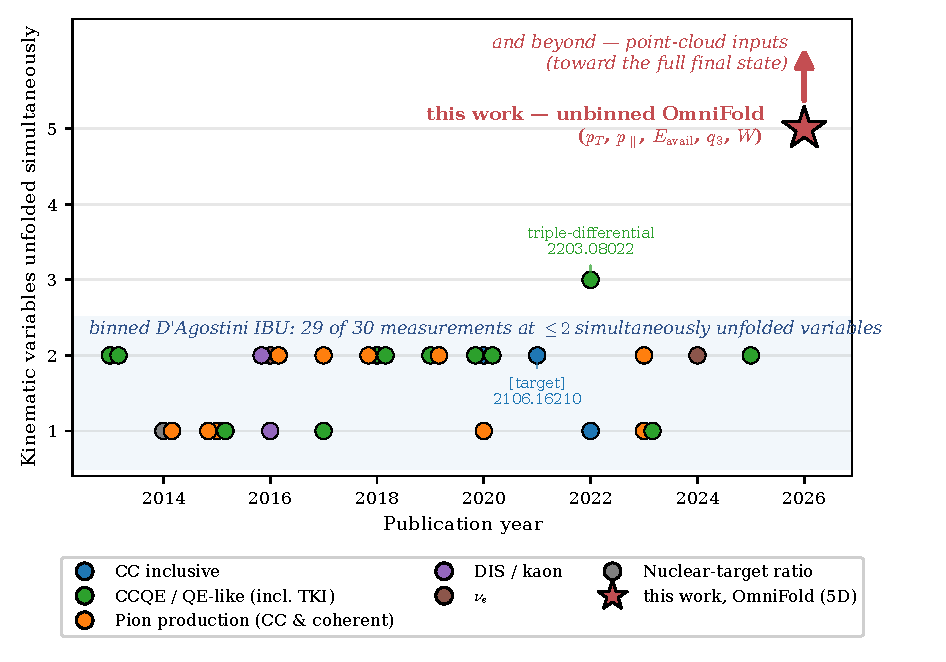
\includegraphics[width=\textwidth]{minerva_unfolding_landscape}
  \caption[Survey of MINERvA differential measurements]{This work unfolds five recorded CC-inclusive high-level observables without binning. Earlier results use binned unfolding, including a triple-differential quasielastic-like measurement. The survey shows MINERvA differential measurements by number of simultaneously unfolded kinematic variables, by year, colored by channel (a double-differential $d^{2}\sigma/dx\,dy$ counts as two). Sources: the MINERvA data-release page and cited publications. The inventory runs through 2025, with newer measurements in App.~\ref{app:landscape}. Classification uses headline differential results, excluding flux, reconstruction, generator-tuning and total-only entries.}
  \label{fig:landscape}
\end{figure}

\section{Data, observables and the unfolding method}\label{recsec:method}
% Generated by records_reorg.py assemble (records-reorg/); edit the data and re-run, not this file.
\subsection{Data, simulation and event selection}\label{recsec:method-data}

% Compression rewrite (DECISION-20261119c; REWRITE-RULES-20261119.md rule 5): text the limitation-resolver lane
% moved verbatim out of the posted note, with one move-manifest row per sentence (LR-C ids in
% history-cuts/move-manifest-lr-20261117.tsv). References into the note resolve through main_note.aux (xr).
% [records reorg] former heading: \section{Method and statistics detail moved from the note}
% [records reorg, not printed] This section holds the procedure and supporting detail that the compressed note no longer prints, as the note printed it.

\paragraph{Per-event analysis trees.}
% [records reorg] former heading: \subsection{Per-event analysis trees (from Part 2, sec:evloop)}
% From sec_experiment.tex:34 (draft f6a4fc372 lineage); procedure a reader does not need to interpret a result
Unbinned unfolding needs per-event records rather than histograms. A dedicated event loop (App.~\ref{app:codebase}), built on MAT's systematic-universe tools, writes four per-event samples for each playlist: all true signal events (the efficiency denominator), reconstructed truth-matched simulated events, simulated background, and data. Entries carry truth and reconstructed observables ($\pT$, $\pPar$, and in extended runs $\Eavail$, $q_{3}$, $W$) and the MINERvA Tune~v1 central-value weight. The systematic-universe samples also carry every universe's weight and the shifted observables of each lateral band, a variation that shifts reconstructed kinematics rather than reweighting events (a vertical band; \S\ref{sec:systematics}). Two conditions make the truth sample the complete reference for the simulated signal:
% (\texttt{\_universes\_full})
\begin{itemize}
  \item A reconstructed signal event is filled only if its $(\mathrm{run},\mathrm{subrun},\mathrm{event})$ key is in the truth denominator. Truth events without a reconstructed partner enter as native OmniFold ``miss'' entries.
  \item The simulated signal sample is complete by construction at ME~FHC (completeness $c=1.000000$; \S\ref{sec:method-xsec}).
\end{itemize}
The loop reads one playlist-wide flux and calibration from the first event, so it is run separately for each playlist, and the twelve per-playlist outputs are combined. The corresponding baseline histogram event loop supplies the flux histogram, POT-weighted across playlists; the size of the playlist-to-playlist flux differences is stated in \S\ref{rlim:experiment}.
% (\texttt{TTree::SetMaxTreeSize}-aware)

\paragraph{Shapes of the reconstructed control distributions.}
% [records reorg] former heading: \subsection{Shapes of the reconstructed control distributions (from Part 2, sec:controlplots)}
% From sec_experiment.tex:49 (draft f6a4fc372 lineage); description of the control figures beyond their captions
The beam and acceptance set the shapes. The $\pPar$ peak at $4$--$6$~GeV/$c$ reflects the ${\langle E_\nu\rangle}\approx\SI{6}{GeV}$ NuMI medium-energy peak; spectrometer matching removes the lowest-$\pPar$ muons. The $\pT$ spectrum peaks near $0.7$~GeV/$c$ and falls by over an order of magnitude across the measured range. Low-recoil (quasi-elastic and $2p2h$) events dominate the sample. Available energy $\Eavail$ concentrates below ${\sim}\SI{0.5}{GeV}$, with a long inelastic tail in the wide upper bins; $q_{3}$ tracks this population's momentum transfer. Reconstructed $W$ rises through the smeared quasi-elastic and $\Delta(1232)$ region before the deep-inelastic continuum takes over above ${\sim}\SI{2}{GeV}$. Absolute background is at the few-percent level under the muon projections and concentrates at high recoil (highest $\Eavail$, $q_{3}$ and $W$ bins).

\paragraph{Detector layout and muon spectrometer.}
% [records reorg] former heading: \subsection{From Part 2, secexperiment.tex: the paragraph beginning ``MINERvAciteMINERvA:2013zvz was a fine-grained scintillator-tracker neutrino''}
% From sec_experiment.tex:5 @d55f7aad6; qualifier detail or procedure (DECISION-20261120a, second pass)
In the paragraph as the note printed it, this text followed: ``MINERvA~\cite{MINERvA:2013zvz} was a fine-grained scintillator-tracker neutrino experiment on Fermilab's NuMI beamline.''\par
Its central tracker comprises hexagonal planes of triangular polystyrene scintillator strips in three stereo orientations, surrounded by electromagnetic and hadronic calorimetry. The magnetized MINOS near detector, \SI{2}{m} downstream, serves as the muon spectrometer, measuring momentum and charge for MINOS-matched tracks.

\paragraph{Reweighting components of the reference simulation.}
% [records reorg] former heading: \subsection{From Part 2, secexperiment.tex: the paragraph beginning ``The reference simulation uses GENIE 2.12.6citeAndreopoulos:2009rq''}
% From sec_experiment.tex:10 @d55f7aad6; qualifier detail or procedure (DECISION-20261120a, second pass)
In the paragraph as the note printed it, this text followed: ``The reference simulation uses GENIE 2.12.6~\cite{Andreopoulos:2009rq} and MINERvA Tune v1, applied as per-event weights by the reweighting tools of the MINERvA Analysis Toolkit (MAT).''\par
These are the flux-and-central-value (flux-and-CV) weight, the GENIE model-parameter (``dial'') weights, the low-recoil 2p2h enhancement fit, and the non-resonant-pion reduction.

\paragraph{Background subtraction before unfolding.}
% [records reorg] former heading: \subsection{From Part 2, secexperiment.tex: the paragraph beginning ``Genuine backgrounds are selected events whose''}
% From sec_experiment.tex:26 @d55f7aad6; qualifier detail or procedure (DECISION-20261120a, second pass)
In the paragraph as the note printed it, this text followed: ``Out-of-phase-space signal, reconstructed inside the phase space with its true muon outside it, is routed into the background template with them.''\par
Both are POT-scaled and subtracted from the reconstructed-data target before unfolding (\S\ref{sec:method}). Their sum, $N_{\mathrm{bkg}}(b)$ in each reconstructed bin, enters the purity weight $w_{\mathrm{pur}}(b)$ of \S\ref{sec:method-algo}.

\paragraph{Composition of the background template.}
% [records reorg] former heading: \subsection{From Part 2, secexperiment.tex: the paragraph beginning ``The background template used for this''}
% From sec_experiment.tex:28 @d55f7aad6; qualifier detail or procedure (DECISION-20261120a, second pass)
% [lead-in, Option B] In the paragraph as the note printed it, this text followed: ``The background template used for this result is \SI{2.91}{\percent} of selected data events in the two-dimensional grid over the full sample (\SIrange{2.72}{3.23}{\percent} per playlist, \SI{2.74}{\percent} on playlist 1A).''\par
On playlist 1A only, about \SI{10}{\percent} (weighted) of the template is out-of-phase-space signal. These are $\nu_{\mu}$ charged-current events with a true vertex inside the fiducial volume. The rest is genuine background, mostly $\nu_{\mu}$ charged-current events with a true vertex outside it.

\paragraph{Data-to-simulation normalization at reconstructed level.}
% [records reorg] former heading: \subsection{From Part 2, secexperiment.tex: the paragraph beginning ``Selected data exceed the POT-scaled MINERvA''}
% From sec_experiment.tex:39 @d55f7aad6; qualifier detail or procedure (DECISION-20261120a, second pass)
Selected data exceed the POT-scaled MINERvA Tune~v1 prediction (signal $+$ background) by $\sim\SI{12}{\percent}$ in overall normalization.
% [records reorg] former heading: \subsection{From Part 2, secexperiment.tex: the paragraph beginning ``Selected data exceed the POT-scaled MINERvA''}
% From sec_experiment.tex:39 @d55f7aad6; qualifier detail or procedure (DECISION-20261120a, second pass)
% [lead-in, Option B] In the paragraph as the note printed it, this text followed: ``The data/MC ratio rises with $\pT$, from $0.88$ in the lowest bin to $\sim1.2$ above \SI{1}{GeV/c}.''\par
Excess and trend together reflect the truth-level normalization deficit of \S\ref{sec:results-model} and \S\ref{sec:3d-models}. Beyond the $\pT$ trend noted above, the ratio panels also show a mild enhancement in the lowest $\Eavail$ bins, reflecting the low-recoil excess examined at truth level in \S\ref{sec:3d-2p2h}.

\paragraph{Status of the PET method.}
% [records reorg] former heading: \subsubsection{From Part 2, the selection-and-classifier table caption (row n06)}
% From selection_features.tex:6 @e89694209; register row, check stage 2026-11-21
% absence-ok: verbatim move of a register sentence; the note's PET pointer is sec6_conclusions.tex (point-cloud event representations)
% [lead-in, Option B] In the paragraph as the note printed it, this text followed: ``Selection and classifier information are separate choices. Reporting bins are not classifier inputs.''\par
PET remains diagnostic method development; its design-study recovery does not validate real-data background subtraction.

\subsection{Observable definitions}\label{recsec:method-observables}

\paragraph{Truth-level W residual.}
% [records reorg] former heading: \subsection{Truth-level W residual (from Part 2, the five observables)}
% From sec_observables.tex:40 (draft f6a4fc372 lineage); detail a reader does not need to interpret a result
At truth level, $q_{3}$ is computed from the true neutrino and muon four-vectors, but $\theta_{\mu}$, and with it $\pT$ and $\pPar$, is measured from a fixed beam axis tilted by \SI{58.87}{mrad} from the detector axis rather than from the true neutrino direction.  Truth $W$ is therefore fixed by $(\pT,\pPar,q_{3})$ only up to that event-by-event angle, of about \SI{1}{mrad}, and the choice of $M$: the residual is within \SI{\pm2}{MeV} for 68\% of events and within $-49$ to $+67$~MeV for 99.9\%; \SI{0.25}{\percent} of events (weighted) change their coarse $W$ bin, and \SI{0.086}{\percent} (weighted) have no real solution. % D1 (crossdoc audit 2026-11-15): weighted, probe_omni.json:10 q3sq_minus_pt2_negative_wfrac 0.0008646 (the 0.15% was the unweighted 49754/32846302, :9 and :8); the Supplement prints m4w-noreal-pct, 0.086
% Methods rewrite (M4, the truth-W residual): M4-W-RECORD.md :6 (theta_true from a fixed beam axis tilted -58.87 mrad
% about x, MAT TruthFunctions.h:21-27, PlotUtilsPhysicalConstants.h:44), :7 and :74-81 (W_true - W_pred with M_bar: 68%
% within about +-2 MeV, 99.9% within -49/+67 MeV), :85-90 (0.25% of events, weighted, change coarse W bin; 0.15% have
% no real solution), :63 (the tilt is the only other cause), :55-59 (median 1.03 mrad between the true neutrino and that
% axis); q3 from the true four-vectors, README-gen5d-build.md:50-58. REVIEW-1 finding 18: M4-W-RECORD.md:7, :72.

\paragraph{Energy transfer $q_{0}$.}
% [records reorg] former heading: \subsection{From Part 2, secobservables.tex: the paragraph beginning ``Tablereftab:observables-impl gives the implemented truth and''}
% From sec_observables.tex:6 @d55f7aad6; qualifier detail or procedure (DECISION-20261120a, second pass)
% [lead-in, Option B] In the paragraph as the note printed it, this text followed: ``$E_{\mu}$, $p_{\mu}$, and $\theta_{\mu}$ are the muon energy, momentum, and angle.''\par
$q_{0}$ is the calorimetric estimate of the energy transfer.

\paragraph{Classifier inputs and reported observables.}
% [records reorg] former heading: \subsection{From Part 2, secobservables.tex: the paragraph beginning ``The five reconstructed inputs therefore share''}
% From sec_observables.tex:41 @d55f7aad6; qualifier detail or procedure (DECISION-20261120a, second pass)
% [lead-in, Option B] In the paragraph as the note printed it, this text followed: ``The five reconstructed inputs therefore share information and do not, by themselves, provide five independent constraints: the result is five simultaneous observables, not five independent measurements.''\par
The five classifier inputs, the lower-dimensional support they populate, and the five reported observables are distinct. Only reconstructed $W$ is fixed by the other inputs; reconstructed $\Eavail$ comes from a separate calorimetric estimator and is not a function of them. The nearly degenerate correlation directions of the joint-test metric (\S\ref{sec:joint5d-design}) are consistent with this redundancy, but that origin has not been shown, and the information added by $W$ has not been measured.
% carried with the text from sec_observables.tex:42 @d55f7aad6
% absence-ok: "has not been shown" and "has not been measured" are the base's own limitations of the five inputs, reworded in r22 Step 2

\paragraph{Effect of the sample-definition convention on cells.}
% [records reorg] former heading: \subsection{From Part 2, secobservables.tex: the paragraph beginning ``The analysis excludes events with negative''}
% From sec_observables.tex:44 @d55f7aad6; qualifier detail or procedure (DECISION-20261120a, second pass)
% [lead-in, Option B] In the paragraph as the note printed it, this text followed: ``The generators measure $\pT$ and $\pPar$ about their own neutrino axis; their $\pT$ differs from the analysis truth $\pT$ by \SI{\pm4}{MeV} for 68\% of events.''\par
Over the 109 joint-test cells, this convention changes the analysis simulation's cell contents by factors between 0.9965 and 1.0035 (median 1.000008), at the level of its Monte Carlo precision, and shifts GENIE's central prediction by between $-0.47$ and $+0.53$ of each cell's null standard deviation.
% carried with the text from sec_observables.tex:45 @d55f7aad6
% Search: information added by W; W redundancy; near-degenerate directions; origin; joint-test metric; pT axis; neutrino axis; beam axis; MP-5; R_c (none for W's information or the origin: M2-ARCHIVE-CHECKS.md:7, r12/ledger.md:103-104 restate it; the pT-axis effect is printed from MP-5, state/measurement-paper/phase1/mp5/REPORT.md:66, :68, :100, job 60017887, with its transfer to the other generators UNRELIABLE, :87-90; Joseph, DECISION-20261027-joseph-absence-audit-items-3-4.md item 1) @ 7a6ae651

\paragraph{Charged-pion mass replacement in $E_{\mathrm{avail}}$.}
% [records reorg] former heading: \subsubsection{From Part 2, the charged-pion offset in the available energy}
% From sec_3d.tex:36 @e89694209; check-stage claims read
% Search: 135 MeV; 139.57; mass_pion; pion mass; OI-30; UD-002 (stands: DECISION-20261101-joseph-eavail-keep-135.md item 1); materiality; covariance projection (done for the sixteen-cell result: ASSESSMENT-20261031-eavail-charged-pion-mass-switch-pricing.md sec. 7.3, full-covariance norm 0.43 prior level / 0.42 first order; EAVAIL_DEFINITION.md sec. 3 as corrected by #637) @ c93a73bce
% [lead-in, Option B] In the paragraph as the note printed it, this text followed: ``The charged-pion term subtracts the inherited constant \SI{135}{MeV} instead of the charged-pion mass of about \SI{139.57}{MeV}.''\par
Relative to the charged-pion mass, it moves \fvval{eavbin-share}\,\% of simulated signal weight to other bins on the fine grid of seven true-$\Eavail$ bins and changes none of the seven bins by more than \fvval{eavbin-max}\,\%. This effect has not been assessed against the projected five-dimensional covariance of the \resFiveAxis{} from the \estPurity{} (estimator definitions, Table~\ref{tab:estimators-matrix}). We tested the mass replacement on the \resSixteen{} (Sec.~\ref{sec:fived16}) from the \estMultiD{}. The cross section shifts by at most \fvval{eav-cellmax}$\sigma$ in any cell. The coherent shift has norm \fvval{eav-coherent}$\sigma$ under the reported covariance.

\paragraph{Generator neutrino axis for muon kinematics.}
% [records reorg] former heading: \subsubsection{From Part 2, the generators' muon axis}
% From sec_observables.tex:44 @e89694209; check-stage claims read
The generators measure $\pT$ and $\pPar$ about their own neutrino axis; their $\pT$ differs from the analysis truth $\pT$ by \SI{\pm4}{MeV} for 68\% of events. For GENIE with MEC, NuWro and GiBUU its effect is not reliably determined (Ref.~\cite{NoteRecords2026}, \recentry{mp5-truth-axis}).

\subsection{The OmniFold implementation and its training settings}\label{recsec:method-omnifold}

\paragraph{Iteration count and the Huang et al.\ recommendation.}
% [records reorg] former heading: \subsection{Iteration count and the Huang et al.\ recommendation (from Part 2, sec:method-config)}
% From sec_method.tex (dfc41cdf5) (draft f6a4fc372 lineage); rationale a reader does not need to interpret a result
Huang \emph{et al.}~\cite{Huang:2025omnifold} select 45 iterations for OmniFold-family methods (20 for their binned benchmark) using a binned $\chi^{2}$ against known mock-data truth, a criterion they note is infeasible on real data. We do not adopt that recommendation. Their mock data injects a large prior--data \emph{shape} discrepancy through an RPA-modified quasielastic model, requiring many iterations. The simulation prior differs from the measured distributions in shape as well as normalization: the data exceed it by about 12\%, and the data/MC ratio rises with $\pT$ from 0.88 to about 1.2 (\S\ref{sec:controlplots}). Cross-experiment production also typically uses ${\sim}5$ iterations~\cite{Canelli:2025guide}.

\paragraph{MINERvA driver and pipeline conventions.}
% [records reorg] former heading: \subsection{MINERvA driver and pipeline conventions (from Part 2, sec:method-driver)}
% From sec_method.tex (dfc41cdf5) (draft f6a4fc372 lineage); procedure a reader does not need to interpret a result
The higher-dimensional MINERvA driver (App.~\ref{app:codebase}) extends the 2D driver using an axis list and the same 2D helpers. The first two axes are always $(\pT,\pPar)$, carrying the fiducial phase-space cut and the per-$\pT$ flux. Higher-dimensional runs extend the muon observables $(\pT,\pPar)$ with $\Eavail$, $q_{3}$, $W$ in the phase space of \S\ref{sec:selection}. Every production, universe-sweep, and closure run follows these conventions:
\begin{itemize}[itemsep=2pt]
  \item \textbf{Reco-space masking.} The measured events entering step-1 training are exactly those passing the reconstructed-level selection; nothing outside the reconstructed phase space reaches the classifier.
  \item \textbf{Step-1 training within the phase space.} Step 1 targets the background-subtracted data of \S\ref{sec:method-algo}, purity-weighted or with background simulation injected at negative weight (refined to non-negative weights in the refined configurations). Genuine backgrounds \emph{and} out-of-phase-space signal are removed from the data side. The simulated reconstructed sample contains no out-of-phase-space signal by construction, so neither side of the step-1 training contains events whose truth lies outside the measurement phase space.
        % Accuracy fix (unscored; director ruling 2026-10-26): the list covers every production run, and the 2D result
        % and the 3D and 4D central values use refined negative-weight subtraction (sec:method-algo). Mechanism:
        % 2d-unfolding/unfold_2d_omnifold_unbinned.py:1362-1377 and :1825-1870 @ ddf16f10; nd-unfolding/unfold_nd_omnifold_unbinned.py:619-630 and :900-1030 @ ddf16f10.
        % In the negative-weight modes the signal fakes are injected with the background (2d-unfolding/unfold_2d_omnifold_unbinned.py:1846-1858 @ ddf16f10).
  \item At histogramming, each simulated truth event carries its final OmniFold push-weight times its central-value simulation weight, including MINERvA Tune~v1 reweighting. No efficiency-histogram division is applied: the step-1 regression for unreconstructed truth events already gives an efficiency-corrected truth spectrum, and dividing again would double-correct.
        % Development history: a failure mode that occurred once in
        % development and was caught by the marginal self-validation gate
        % (\S\ref{sec:validation}).
  \item \textbf{Closure mirrors production.} In closure tests the pseudo-data are simulated events passing both the reconstructed and truth selections, weighted identically to the production data path, so closure exercises the same code path as the data unfolding.
\end{itemize}

\paragraph{Step-1 weights for missed truth events.}
% [records reorg] former heading: \subsection{From Part 2, secmethod.tex: the paragraph beginning ``item textbfStep 1 (detector space). A''}
% From sec_method.tex:9 @d55f7aad6; qualifier detail or procedure (DECISION-20261120a, second pass)
% [lead-in, Option B] In the paragraph as the note printed it, this text followed: ``The weight is \emph{pulled back} directly to its truth record.''\par
Truth events without a reconstructed partner (``misses'') receive step-1 weights from a regressor trained on the reconstructed subsample, $w(\mathrm{truth\ features})$. This native OmniFold acceptance treatment requires no separate efficiency correction.

\paragraph{Adding observables in unbinned OmniFold.}
% [records reorg] former heading: \subsection{From Part 2, secmethod.tex: the paragraph beginning ``Unbinned OmniFold adds an observable by''}
% From sec_method.tex:14 @d55f7aad6; qualifier detail or procedure (DECISION-20261120a, second pass)
Unbinned OmniFold adds an observable by adding an input to the step-1 and step-2 classifiers, without an explicit migration matrix or per-bin response tensor. It avoids the combinatorial binning penalty of matrix unfolding but still has a dimensional cost: classifier training, acceptance and support coverage, sample sparsity and uncertainty quantification become more demanding as observables are added. The primary methodological motivation is the absence of a practical analog of D'Agostini iterative Bayesian unfolding (IBU).

\paragraph{Gradient-boosted decision trees as classifiers.}
% [records reorg] former heading: \subsection{From Part 2, secmethod.tex: the paragraph beginning ``Gradient-boosted decision trees (GBDTs) replace OmniFold's''}
% From sec_method.tex:50 @d55f7aad6; qualifier detail or procedure (DECISION-20261120a, second pass)
Gradient-boosted decision trees (GBDTs) replace OmniFold's original neural networks when unfolding scalar observables. With at most five high-level features per event, tree ensembles typically match or outperform neural networks~\cite{Grinsztajn:2022tabular} and train deterministically and far faster on a central processing unit (CPU). All unfolding results here use GBDTs (point-cloud representations, App.~\ref{sec:pet}). Calibration tests and multilayer perceptron (MLP) cross-checks test the implementation (classifier checks, \S\ref{sec:3d-classifier}).

\paragraph{Learner of the quoted 2D central value.}
% [records reorg] former heading: \subsection{From Part 2, secmethod.tex: the paragraph beginning ``The unfolding code supports interchangeable learners''}
% From sec_method.tex:52 @d55f7aad6; qualifier detail or procedure (DECISION-20261120a, second pass)
The unfolding code supports interchangeable learners (component terminology and code paths in App.~\ref{app:codebase}). The quoted 2D central value and all its uncertainty ensembles use LightGBM with refined negative-weight subtraction (background method, App.~\ref{app:negweight}). The estimator matrix (Table~\ref{tab:estimators-matrix}) lists this as the \estTwoD{}. The ensembles cover the systematic-universe sweep, Poisson bootstrap, training-seed variations and run-period unfoldings.
% [records reorg] former heading: \subsection{From Part 2, secmethod.tex: the paragraph beginning ``The unfolding code supports interchangeable learners''}
% From sec_method.tex:52 @d55f7aad6; qualifier detail or procedure (DECISION-20261120a, second pass)
% [lead-in, Option B] In the paragraph as the note printed it, this text followed: ``The step-1 classifier, the step-2 classifier and the regressor for unreconstructed truth events share one setting: $100$ trees, $8$ leaves and learning rate $0.1$.''\par
The universe sweep supplies the central value at seed~42. Thus the systematic covariance shares its estimator and seed (systematic universes, \S\ref{sec:uq-universes}). The quoted statistical covariance also uses seed~42, with three independent bootstrap streams (data, signal and background simulation, \S\ref{sec:uq-boot}). The training-seed covariance uses five seed settings that include seed~42 (\S\ref{sec:uq-ml}).

\paragraph{Reproducibility and seed dispersion of the central value.}
% [records reorg] former heading: \subsection{From Part 2, secmethod.tex: the paragraph beginning ``A central unfolding at seed45 differs''}
% From sec_method.tex:54 @d55f7aad6; qualifier detail or procedure (DECISION-20261120a, second pass)
In the paragraph as the note printed it, this text followed: ``A central unfolding at seed~45 differs from the seed-42 one by at most \SI{1.4}{\percent} in a cell.''\par
The quoted central value has a recorded configuration and repeats numerically. It agrees with the refined 2D data unfolding (background study, App.~\ref{sec:negweight-footing}).
% carried with the text from sec_method.tex:55 @d55f7aad6
% Source: docs/publication/DECISION-20261011-joseph-2d-central-lightgbm-seed42.md; receipts
% [records reorg] former heading: \subsection{From Part 2, secmethod.tex: the paragraph beginning ``A central unfolding at seed45 differs''}
% From sec_method.tex:54 @d55f7aad6; qualifier detail or procedure (DECISION-20261120a, second pass)
% [lead-in, Option B] In the paragraph as the note printed it, this text followed: ``The purity-subtracted seed-42 central value has no recorded run configuration, although an independent rerun and a regeneration whose run configuration is recorded both reproduce it (Ref.~\cite{NoteRecords2026}, \recentry{2d-central-value}).''\par
Against the ten purity-subtracted LightGBM central values at seeds 1--10 it is mildly over-dispersed (root-mean-square standardized difference 1.28, maximum 4.25). The choice of seed~42 is recorded in App.~\ref{app:devhistory}.
% carried with the text from sec_method.tex:55 @d55f7aad6
% Source: docs/publication/DECISION-20261011-joseph-2d-central-lightgbm-seed42.md; receipts

\paragraph{Multidimensional estimator settings.}
% [records reorg] former heading: \subsection{From Part 2, secmethod.tex: the paragraph beginning ``paragraphHyperparameter choice. Neither OmniFold classifier nor''}
% From sec_method.tex:144 @d55f7aad6; qualifier detail or procedure (DECISION-20261120a, second pass)
The \estMultiD{} keeps five iterations under the precision study's rule (\S\ref{sec:gbdt-model-dependence}). Its refinement classifier, 400 trees and 31 leaves, was selected before the joint-test design was fixed (\S\ref{sec:joint5d}).

\paragraph{Fixed GBDT settings and capacity.}
% [records reorg] former heading: \subsection{From Part 2, secmethod.tex: the paragraph beginning ``The fixed settings are the scikit-learn''}
% From sec_method.tex:146 @d55f7aad6; qualifier detail or procedure (DECISION-20261120a, second pass)
The fixed settings are the scikit-learn \texttt{GradientBoosting} defaults: 100 trees, learning rate $0.1$, and depth-3 capacity. The LightGBM learner of the central value and its ensembles uses matched capacity ($\texttt{num\_leaves}=8=2^{3}$), so both have the same deliberately modest capacity, an OmniFold regularizer (algorithm, \S\ref{sec:method-algo}).

\paragraph{Keras multilayer-perceptron cross-check.}
% [records reorg] former heading: \subsection{From Part 2, secmethod.tex: the paragraph beginning ``The Keras cross-check (Srefsec:3d-classifier) uses the''}
% From sec_method.tex:150 @d55f7aad6; qualifier detail or procedure (DECISION-20261120a, second pass)
The Keras cross-check (\S\ref{sec:3d-classifier}) uses the same multilayer perceptron for both classifiers and missed-event regression. It has three hidden layers of 64, 128 and 64 units and Gaussian error linear unit (GELU) activation. Training uses Adam for at most 50 epochs with early stopping, per-fit input standardization and a fixed shuffle. Settings stay fixed. Agreement does not address sensitivity to single-precision (float32) ties (departure tests, \S\ref{sec:val-departure}).

\paragraph{Performance diagnostics.}
% [records reorg] former heading: \subsection{From Part 2, secmethod.tex: the paragraph beginning ``The following diagnostics report performance. They''}
% From sec_method.tex:152 @d55f7aad6; qualifier detail or procedure (DECISION-20261120a, second pass)
% [lead-in, Option B] In the paragraph as the note printed it, this text followed: ``The following diagnostics report performance. They do not validate the quoted estimator or its intervals. They include closure tests (\S\ref{sec:validation}) and classifier calibration (\S\ref{sec:3d-classifier}).''\par
The exact-split cross-check measures insensitivity to doubling the iterations (below). Method-dependence studies report backend agreement (\S\ref{sec:results-tension}). The training-seed variation band measures residual machine-learning (ML) stochasticity (\S\ref{sec:systematics}).

\paragraph{Iteration count.}
% [records reorg] former heading: \subsection{From Part 2, secmethod.tex: the paragraph beginning ``Production uses n=5 iterations. Between five''}
% From sec_method.tex:154 @d55f7aad6; qualifier detail or procedure (DECISION-20261120a, second pass)
Production uses $n=5$ iterations.
% [records reorg] former heading: \subsection{From Part 2, secmethod.tex: the paragraph beginning ``Production uses n=5 iterations. Between five''}
% From sec_method.tex:154 @d55f7aad6; qualifier detail or procedure (DECISION-20261120a, second pass)
% [lead-in, Option B] In the paragraph as the note printed it, this text followed: ``Between five and ten iterations, the exact-split total cross section agrees to within \SI{0.026}{\percent} (validation, \S\ref{sec:validation}). That measures movement of this diagnostic for that cross-check. It does not establish convergence of every functional.''\par
Separately, the unfolded result reproduces the integrated cross section of an independently published binned measurement of the same data (results, \S\ref{sec:results}). That comparison is not an iteration test.

\paragraph{Inputs to the step-1 classifier.}
% [records reorg] former heading: \subsection{From Part 2, secmethod.tex: the paragraph beginning ``Every production, universe-sweep and closure run''}
% From sec_method.tex:164 @d55f7aad6; qualifier detail or procedure (DECISION-20261120a, second pass)
% [lead-in, Option B] In the paragraph as the note printed it, this text followed: ``Every production, universe-sweep and closure run follows the same pipeline conventions (records document, Ref.~\cite{NoteRecords2026}).''\par
Only events passing reconstructed-level selection reach the step-1 classifier.
% [records reorg] former heading: \subsection{From Part 2, secmethod.tex: the paragraph beginning ``Every production, universe-sweep and closure run''}
% From sec_method.tex:164 @d55f7aad6; qualifier detail or procedure (DECISION-20261120a, second pass)
% [lead-in, Option B] In the paragraph as the note printed it, this text followed: ``Both sides of step-1 training exclude events with truth outside the measurement phase space.''\par
Closure pseudo-data follow the production data path.

\paragraph{Class weights and effective sample size.}
% [records reorg] former heading: \subsection{From Part 2, secmethod.tex: the paragraph beginning ``paragraphTraining details. Each classifier is trained''}
% From sec_method.tex:17 @fdd67e926; training detail (DECISION-20261120a records route; the director 2026-11-20)
The two classes keep their physical weights, with no class balancing and no renormalization between iterations. The learned ratio $p/(1-p)$ therefore carries the normalization, with $p$ restricted to $[10^{-6},1-10^{-6}]$.
% [records reorg] former heading: \subsection{From Part 2, secmethod.tex: the paragraph beginning ``paragraphTraining details. Each classifier is trained''}
% From sec_method.tex:17 @fdd67e926; training detail (DECISION-20261120a records route; the director 2026-11-20)
% [lead-in, Option B] In the paragraph as the note printed it, this text followed: ``In the refined configurations, a classifier separating positive from negative weights, trained with $|w|$, gives each event the weight $|w|\max(0,2g-1)$.''\par
For the \estMultiD{}, the per-event Kish effective sample size and weight tails have been computed on the sixteen reported cells~\cite{UnfoldedWeightsESS2026}. They describe the unfolded simulated-event weights and are not an uncertainty, coverage or validity statement.

\paragraph{Check-stage moves at the journal-voice rewrite (2026-11-21).}
% [records reorg] former heading: \subsection{Check-stage moves at the journal-voice rewrite (2026-11-21)}
% Limitation-register rows whose sentence the rewritten note (982945a0a) no longer states, moved verbatim from the
% previous note (draft e89694209) under DECISION-20261120a; one move-manifest row each (LR-K ids in
% history-cuts/move-manifest-lr-check-20261121.tsv). The rewritten note states each result's headline limit.

\paragraph{Alternative-seed central unfolding.}
% [records reorg] former heading: \subsubsection{From Part 2, the training settings (row n07)}
% From sec_method.tex:54 @e89694209; register row, check stage 2026-11-21
% [lead-in, Option B] In the paragraph as the note printed it, this text followed: ``The step-1 classifier, the step-2 classifier and the regressor for unreconstructed truth events share one setting: $100$ trees, $8$ leaves and learning rate $0.1$.''\par
A central unfolding at seed~45 differs from the seed-42 one by at most \SI{1.4}{\percent} in a cell.

\paragraph{Disclosures cut at the journal-voice rewrite (check stage, 2026-11-21).}
% [records reorg] former heading: \subsection{Disclosures cut at the journal-voice rewrite (check stage, 2026-11-21)}
% Qualifications and post-hoc accounts that the check-stage claims reads (Grok, codex2) found the rewritten note no longer
% states, moved verbatim from the previous note (draft e89694209); the rewritten note keeps each result's headline limit.
% One move-manifest row per sentence (LR-K ids, history-cuts/move-manifest-lr-check-20261121.tsv).

\paragraph{Missed-event regressor variants and transfer probe.}
% [records reorg] former heading: \subsubsection{From Part 2, the missed-event regressor and the transfer probe}
% From sec_method.tex:17 @e89694209; check-stage claims read
% absence-ok: scopes what RSN's WR tested (its record's scope: "does not attribute F0b's flags"; the half-sample flags' attribution is T3's, not run), as the paper's limitation 3 at 5bbb9d269 states it
% [lead-in, Option B] In the paragraph as the note printed it, this text followed: ``Truth events without a reconstructed partner receive the prediction of an unweighted regressor of the step-1 weight on the truth observables.''\par
A regressor weighted with each event's current weight instead moves the sixteen-cell data result (\S\ref{sec:fived16}) by at most \fvval{rsn-wr-sig-max} of a cell's reported standard deviation. In noise-free, signal-only closures on the full simulation, it leaves the bias flags at the GiBUU hybrid truth and the $q_3$ tilt unchanged. Its effect on the flags from half-sample pseudo-data with background and noise was not tested. A held-out transfer probe among matched events at fixed truth places no cell beyond half its reported standard deviation, at the data or at those two truths. It cannot show that the missed events resemble matched events in what the five features omit.

\paragraph{Hyperparameter choice.}
% [records reorg] former heading: \subsubsection{From Part 2, the hyperparameter choice}
% From sec_method.tex:144 @e89694209; check-stage claims read
Neither OmniFold classifier nor the missed-event regressor underwent a hyperparameter search on data.

\paragraph{Qualifications from the second check-stage claims read (2026-11-21).}
% [records reorg] former heading: \subsection{Qualifications from the second check-stage claims read (2026-11-21)}
% Moved verbatim from the previous note (draft e89694209); LR-K ids in history-cuts/move-manifest-lr-check-20261121.tsv.

\paragraph{Check-stage moves at the journal-voice rewrite (2026-11-21).}
% [records reorg] former heading: \subsection{Check-stage moves at the journal-voice rewrite (2026-11-21)}
% Limitation-register rows whose sentence the rewritten note (982945a0a) no longer states, moved verbatim from the
% previous note (draft e89694209) under DECISION-20261120a; one move-manifest row each (LR-K ids in
% history-cuts/move-manifest-lr-check-20261121.tsv). The rewritten note states each result's headline limit.

\paragraph{Disclosures cut at the journal-voice rewrite (check stage, 2026-11-21).}
% [records reorg] former heading: \subsection{Disclosures cut at the journal-voice rewrite (check stage, 2026-11-21)}
% Qualifications and post-hoc accounts that the check-stage claims reads (Grok, codex2) found the rewritten note no longer
% states, moved verbatim from the previous note (draft e89694209); the rewritten note keeps each result's headline limit.
% One move-manifest row per sentence (LR-K ids, history-cuts/move-manifest-lr-check-20261121.tsv).

\paragraph{Qualifications from the second check-stage claims read (2026-11-21).}
% [records reorg] former heading: \subsection{Qualifications from the second check-stage claims read (2026-11-21)}
% Moved verbatim from the previous note (draft e89694209); LR-K ids in history-cuts/move-manifest-lr-check-20261121.tsv.

\subsection{Background subtraction in the unfolding}\label{recsec:method-background}

\paragraph{Background subtraction (App.~B): detail.}
% Moved verbatim from app_negweight.tex @ a1e6ec190 in the compression under DECISION-20261120a (qualifier and procedure detail
% may move to the records with a pointer); move-manifest-je JE-20.
% [records reorg] former heading: \subsection{Background subtraction (App.~B): detail moved from the note}

\paragraph{Absence of injected negative weights.}
% [records reorg] former heading: \subsection{From Part 2, secmethod.tex: the paragraph beginning ``paragraphBackground subtraction. In binned purity subtraction,''}
% From sec_method.tex:21 @d55f7aad6; qualifier detail or procedure (DECISION-20261120a, second pass)
No negative-weight events are injected.

\paragraph{Refined and binned subtraction variants.}
% [records reorg] former heading: \subsection{From Part 2, secmethod.tex: the paragraph beginning ``For other experiments' subtraction methods, see''}
% From sec_method.tex:32 @d55f7aad6; qualifier detail or procedure (DECISION-20261120a, second pass)
For other experiments' subtraction methods, see \S\ref{sec:intro}.
% [records reorg] former heading: \subsection{From Part 2, secmethod.tex: the paragraph beginning ``For other experiments' subtraction methods, see''}
% From sec_method.tex:32 @d55f7aad6; qualifier detail or procedure (DECISION-20261120a, second pass)
In the paragraph as the note printed it, this text followed: ``A fully unbinned alternative adds negative-weight background simulation on the measured side.''\par
Its bin-integrated target is $(D_{b}-B_{b})/S_{b}$ (data, background and signal).
% [records reorg] former heading: \subsection{From Part 2, secmethod.tex: the paragraph beginning ``For other experiments' subtraction methods, see''}
% From sec_method.tex:32 @d55f7aad6; qualifier detail or procedure (DECISION-20261120a, second pass)
In the paragraph as the note printed it, this text followed: ``The alternative reproduces the binned correction to \SI{\nwPctTot}{\percent} on the total two-dimensional (2D) cross section and its systematic and statistical covariances to within \SI{2}{\percent} (subtraction comparison, App.~\ref{app:negweight}).''\par
It removes residual binning dependence and suits the extended-fiducial analysis with larger backgrounds. The quoted 2D result and covariance, 3D and 4D central values, sixteen-cell result and covariance, and studies and tests of the \estLowCap{} and \estMultiD{} use the refined variant. All other quoted cross sections and uncertainties, including the \resFiveAxis{} of the \estPurity{} and the extended-fiducial value, use binned subtraction. The matrix, Table~\ref{tab:estimators-matrix} (configurations, \S\ref{sec:method-config}), links results to configurations.

\paragraph{Estimators of the multidimensional results.}
% [records reorg] former heading: \subsection{From Part 2, secmethod.tex: the paragraph beginning ``The quoted 2D cross section and''}
% From sec_method.tex:48 @d55f7aad6; qualifier detail or procedure (DECISION-20261120a, second pass)
% [lead-in, Option B] In the paragraph as the note printed it, this text followed: ``The quoted 2D cross section and covariance use the \estTwoD{}.''\par
The 3D and 4D central values, the \resSixteen{} and the generator tests use the \estMultiD{}. Both subtract background with negative weights and a 400-tree refinement classifier. They differ in training histogram construction in the LightGBM learner and in deterministic settings. An earlier \estPurity{} is retained for the \resFiveAxis{} and for specified figures and closures. Three other configurations serve only as diagnostic controls in the studies listed in Table~\ref{tab:estimators-matrix}, the matrix of estimator uses and implementations.

\subsection{Estimators, configurations and the exact-split cross-check}\label{recsec:method-estimators}

\paragraph{The exact-split cross-check's eigenmode decomposition.}
% Move pair H3-020 (director-helper-3; move-manifest-h3-20261117.tsv sends): sec_results.tex:148 @ 79a934a41, sentences 2-4,
% verbatim with the source comments :153-154; sec:results-tension keeps sentence 1 and points here.
% [records reorg] former heading: \subsubsection{The exact-split cross-check's eigenmode decomposition (from \S\ref{sec:results})}
\label{app:devhistory-results}
This is the exact-split cross-check's part of the eigenmode decomposition of \S\ref{sec:results-tension}. For the exact-split cross-check, $\chi^{2}$ is larger and distributed differently: its components of magnitude $5$--$6$ lie in moderate-$\lambda$ modes on the low-$\pT$ ridge of the cross-section peak. Its 10 smallest-$\lambda$ modes carry \SI{3}{\percent} of the $\chi^{2}$, and the 73 best-measured directions give $\chi^{2}=291$ ($\chi^{2}/205=1.42$, again divided by the number of reported bins; App.~\ref{sec:tension}). Going from 5 to 10 iterations changes the LightGBM (seed~1) value by a negligible $+0.01$.
% Revision D' 2026-11-06 (referee reads of D, both ACCEPT; Sonnet and the interpreter: print the raw chi2 and the directions kept): docs/orchestration/receipts/2d-lgbm42-20261011/tension_report_exact_control.txt:56 prints "1e-04  1.419  73". Arithmetic: 1.419 x 205 = 290.9; 205 x [1.4185, 1.4195) is in [290.8, 291.0], 291 at three figures.
% Director-added wording correction 2026-11-06, for Joseph's review before merge (not among the two he approved): the truncated chi2 was printed as chi2/ndf, but its divisor is the 205 reported bins, not the directions kept. 2d-unfolding/diagnose_tension.py @ c3dbe30f4 (main): :110 n = int(mask.sum()), the 205 reported bins; :183 and :193 divide every truncated chi2 by n (the same divisor at 56e30b9c9 :108/:181/:191 and at 735c909da). Receipt docs/orchestration/receipts/2d-lgbm42-20261011/tension_report_exact_control.txt:56 ("1e-04  1.419  73"). No number changed.
% Moved verbatim (compression K9, class H: a superseded configuration's detail; move-manifest-je JE-10.028..).

\paragraph{Seed dependence of the exact-split result.}
% [records reorg] former heading: \subsection{From Part 2, secmethod.tex: the paragraph beginning ``paragraphThe exact-split cross-check. The exact-split configuration''}
% From sec_method.tex:85 @d55f7aad6; qualifier detail or procedure (DECISION-20261120a, second pass)
Its seed and run log appear in the development history (App.~\ref{app:devhistory}). The result depends on the estimator seed. A reseeded run (\texttt{random\_state} 1/2/3) moves every bin (median \SI{0.18}{\percent}, maximum \SI{1.6}{\percent}) and gives $\chi^{2}/\mathrm{ndf}=\chiPaperExactSeeded$ (chi-square per degree of freedom). The spread over seeds is unmeasured.
% carried with the text from sec_method.tex:86 @d55f7aad6
% Search: exact-split seed scan; spread over seeds; matched covariance; exact-split bootstrap; P09b @ ddf16f10
% Search: exact-backend seed scan; exact-split seed scan; P09b (pairings.tsv: "no exact-backend seed scan exists") @ 1a015eef
% [records reorg] former heading: \subsection{From Part 2, secmethod.tex: the paragraph beginning ``paragraphThe exact-split cross-check. The exact-split configuration''}
% From sec_method.tex:85 @d55f7aad6; qualifier detail or procedure (DECISION-20261120a, second pass)
% [lead-in, Option B] In the paragraph as the note printed it, this text followed: ``The cross-check has no matched covariance.''\par
No exact-split bootstrap, universe sweep or seed scan exists.
% carried with the text from sec_method.tex:86 @d55f7aad6
% Search: exact-split seed scan; spread over seeds; matched covariance; exact-split bootstrap; P09b @ ddf16f10
% Search: exact-backend seed scan; exact-split seed scan; P09b (pairings.tsv: "no exact-backend seed scan exists") @ 1a015eef
% carried with the text from sec_method.tex:86 @d55f7aad6
% Search: exact-split seed scan; spread over seeds; matched covariance; exact-split bootstrap; P09b @ ddf16f10
% Search: exact-backend seed scan; exact-split seed scan; P09b (pairings.tsv: "no exact-backend seed scan exists") @ 1a015eef

\paragraph{Estimator configurations.}
% [records reorg] former heading: \subsection{From Part 2, secmethod.tex: the paragraph beginning ``paragraphThe estimator configurations. The six estimator''}
% From sec_method.tex:102 @d55f7aad6; qualifier detail or procedure (DECISION-20261120a, second pass)
Each result names its estimator.
% [records reorg] former heading: \subsection{From Part 2, secmethod.tex: the paragraph beginning ``paragraphThe estimator configurations. The six estimator''}
% From sec_method.tex:102 @d55f7aad6; qualifier detail or procedure (DECISION-20261120a, second pass)
``Deterministic'' means fixed seeds and reproducible training.
% [records reorg] former heading: \subsection{From Part 2, secmethod.tex: the paragraph beginning ``paragraphThe estimator configurations. The six estimator''}
% From sec_method.tex:102 @d55f7aad6; qualifier detail or procedure (DECISION-20261120a, second pass)
In the paragraph as the note printed it, this text followed: ``Results from different configurations are not combined.''\par
The \estTwoD{} adds refined negative-weight subtraction to the nominal LightGBM configuration above. It uses the \estMultiD{} refinement classifier at the estimator seed plus three. Its quoted seed-42 central value repeats numerically (above). The \estPurity{} is the same learner with purity-based background subtraction (algorithm, \S\ref{sec:method-algo}). The \estMultiD{}, the estimator of the generator tests, is a deterministic LightGBM variant with the unbinned negative-weight background treatment (background method, App.~\ref{app:negweight}). Its refinement classifier has 400 trees and 31 leaves.
% [records reorg] former heading: \subsection{From Part 2, secmethod.tex: the paragraph beginning ``paragraphThe estimator configurations. The six estimator''}
% From sec_method.tex:102 @d55f7aad6; qualifier detail or procedure (DECISION-20261120a, second pass)
In the paragraph as the note printed it, this text followed: ``The negative-weight treatment reduces the purity method's nominal-truth bias in the highest-$W$ (hadronic invariant mass) column by about an order of magnitude (from 3.5--\SI{4.1}{\percent} with purity subtraction to 0.11--\SI{0.24}{\percent} with negative weights).''\par
This reaches the no-background closure level. The larger refinement classifier removes most of the remaining background-related bias (background and departure tests, \S\S\ref{sec:val-negweight}--\ref{sec:val-departure}). The \estMultiD{} was selected before the joint-test design was fixed (\S\ref{sec:joint5d}). The \estExact{} is described above.

\paragraph{Histogram construction and deterministic training.}
% [records reorg] former heading: \subsection{From Part 2, secmethod.tex: the paragraph beginning ``The estPurity and the estTwoD leave''}
% From sec_method.tex:148 @d55f7aad6; qualifier detail or procedure (DECISION-20261120a, second pass)
The \estPurity{} and the \estTwoD{} leave histogram construction at its default. Bin edges come from the library's default row sample. The training seed affects the result through that sample. The configurations this section calls deterministic set those edges from every training row and enable the library's deterministic training.

\paragraph{Regularization scan of the $\chi^{2}$.}
% [records reorg] former heading: \subsection{From App. A, appstatmethods.tex: the paragraph beginning ``For the exact-split cross-check and an''}
% From app_statmethods.tex:440 @d55f7aad6; qualifier detail or procedure (DECISION-20261120a, second pass)
Each method spans roughly two decades of $\chi^{2}/205$ across a two-decade scan of its regularization parameter, with no defensible single cutoff. The useful conclusion is diagnostic, not a number: the naive inverse is dominated by tiny, poorly-determined modes, and in the retained high-variance modes the central-value difference is not large. We therefore report direct per-bin pulls (\S\ref{sec:pull}) and this scan rather than a single unqualified $\chi^{2}_{\ours}$.

\paragraph{Separation of configurations.}
% [records reorg] former heading: \subsubsection{From Part 2, the estimator configurations (row n09)}
% From sec_method.tex:102 @e89694209; register row, check stage 2026-11-21
% [lead-in, Option B] In the paragraph as the note printed it, this text followed: ``All use five OmniFold iterations and gradient-boosted trees of nominal capacity (100 trees, 8 leaves) in both OmniFold steps.''\par
Results from different configurations are not combined.

\paragraph{Scope of reduced prior dependence.}
% [records reorg] former heading: \subsubsection{From Part 2, related developments and estimator scope (row n13)}
% From sec_method.tex:201 @e89694209; register row, check stage 2026-11-21
% absence-ok: verbatim move of a register sentence (a scoping statement, not an absence of a record)
% [lead-in, Option B] In the paragraph as the note printed it, this text followed: ``See the records for the distinction from Profile OmniFold (Ref.~\cite{NoteRecords2026}).''\par
Reduced simulation-prior dependence does not establish detector-model independence, adequate phase-space support, or coverage for this result.

\paragraph{Exact-split central-value differences.}
% [records reorg] former heading: \subsubsection{From Part 2, the exact-split cross-check}
% From sec_method.tex:85 @e89694209; check-stage claims read
% [lead-in, Option B] In the paragraph as the note printed it, this text followed: ``The exact-split configuration (\texttt{exact}) uses scikit-learn \texttt{GradientBoosting} with single-threaded exact-split classification and regression trees (CART).''\par
The exact-split central value differs from the purity-subtracted LightGBM seed-42 central value by a per-bin median \SI{0.98}{\percent} (maximum \SI{12.2}{\percent}), 1.32 statistical standard deviations. It differs from the quoted central value, which also differs from it in background treatment, by a per-bin median of \SI{1.03}{\percent} (maximum \SI{17.6}{\percent}).
% [records reorg] former heading: \subsubsection{From Part 2, the scope of exact-split studies}
% From sec_method.tex:103 @e89694209; check-stage claims read
In the paragraph as the note printed it, this text followed: ``Studies labeled \emph{exact-split} use that cross-check, an earlier quoted 2D central value.''\par
They have not been repeated for the quoted estimator.

\paragraph{Shape distance of the exact-split cross-check.}
% [records reorg] former heading: \subsubsection{From App. A, the exact-split shape distance}
% From app_statmethods.tex:398 @e89694209; check-stage claims read
For the exact-split cross-check, which as above is not recomputed for the LightGBM central value, with the paper's \texttt{TotalCovariance} (Jacobian-propagated) the shape $\chi^{2}/\mathrm{ndf}$ on $205$ bins is $\boxed{3.596}$: essentially the absolute-normalization $3.661$ \emph{minus} the contribution of overall scale. The total-cross-section ratio $\sigma_{\tot}^{\ours}/\sigma_{\tot}^{\paper} = 1.0111$ is a $1\%$ scale difference. The remaining residual comes from $\sim 1\%$ shape disagreement (median bin ratio $1.0064$; $94\%$ of bins within $10\%$ of the paper).

\paragraph{Relative uncertainties with respect to the exact-split cross-check.}
% [records reorg] former heading: \subsection{Relative uncertainties with respect to the exact-split cross-check (from Part 3, the uncertainty budget)}
% From sec_results.tex:30 @ draft 47c318849, the paragraph's last sentence, with its source comment
Taken with respect to the exact-split cross-check instead, the same combined covariance has a per-bin median of \SI{6.468}{\percent}. % G2R: RE-2-shapes run 2 (C_new), g2r-integration/ledger.tsv g2r-res-q-vs-ec; a source comment citing RE-2 part C for this value gives the earlier value

\subsection{Binning, migrations and the reported product}\label{recsec:method-binning}

\paragraph{Structure of the truth-to-reco migrations.}
% [records reorg] former heading: \subsection{Structure of the truth-to-reco migrations (from Part 2, sec:method-binning)}
% From sec_method.tex (dfc41cdf5) (draft f6a4fc372 lineage); description of the migration figure beyond its caption
The structure differs qualitatively between the muon and hadron sides. The spectrometer muon measurement makes the $\pT$ and $\pPar$ maps nearly tridiagonal, with migrations rarely exceeding one bin. Reconstruction stability dips to ${\sim}0.45$--$0.5$ for $\pT$ and ${\sim}0.35$ for $\pPar$ where bins are finest, recovering in wide edge bins. The calorimetric axes have coarser bins but relatively broader, visibly asymmetric migrations. $\Eavail$ preferentially migrates \emph{downward} because energy carried by neutrons and other unresponsive particles is not collected. Reconstruction stability falls from $0.61$ in the lowest bins to $0.43$ in the highest. $q_{3}$, reconstructed from the muon $Q^{2}$ and the calorimetric recoil, inherits a milder version of the same pattern. $W$ compounds $\Eavail$ and muon smearing and has the broadest migrations; two-bin shifts are common in the resonance region. The lowest-$W$ (quasi-elastic) bin has the highest stability at $0.71$.

\paragraph{No underflow or overflow in the reported product.}
% [records reorg] former heading: \subsection{No underflow or overflow in the reported product (from Part 2, sec:method-binning)}
% From sec_method.tex @1ad08b466; argument a reader does not need to interpret a result
Neither underflow nor overflow appears in the reported product, by construction rather than by truncation: the unbinned unfolding has no response-matrix under- or overflow, and the reporting bins are applied once, to events that all lie inside the grids. Truth-level muon edges coincide with the measurement phase space (\S\ref{sec:selection}); no signal is defined beyond them. Hadronic axes span $[0,100]\,\si{GeV}$, with catch-bin edges far beyond the kinematic reach at $\langle E_\nu\rangle\sim\SI{6}{GeV}$, so the truth grids are exhaustive. A selected reco event outside the grid is treated as unaccepted and excluded from the measured sample by \S\ref{sec:method-driver}'s masking convention. Its in-phase-space truth content is recovered, as for any unreconstructed event, by the treatment of truth events without a reconstructed partner.

\paragraph{Correction factor, self-test and flux integral.}
% [records reorg] former heading: \subsection{From Part 2, secmethod.tex: the paragraph beginning ``In n dimensions, the differential cross''}
% From sec_method.tex:176 @d55f7aad6; qualifier detail or procedure (DECISION-20261120a, second pass)
% [lead-in, Option B] In the paragraph as the note printed it, this text followed: ``Thus the defined truth sample enters and $c\equiv1$ per bin.''\par
Negative truth $W^{2}$ is excluded by the five-observable sample definition (\S\ref{sec:eavailw-definitions}). This differs from losing a reconstructed event from the input. The factor remains a monitored self-check. Dropping unmatched truth events would give $c<1$.
% [records reorg] former heading: \subsection{From Part 2, secmethod.tex: the paragraph beginning ``In n dimensions, the differential cross''}
% From sec_method.tex:176 @d55f7aad6; qualifier detail or procedure (DECISION-20261120a, second pass)
% [lead-in, Option B] In the paragraph as the note printed it, this text followed: ``$\Phi$ is the flux integral by transverse muon momentum $\pT$. It is tabulated per square meter and broadcast over other axes.''\par
The formula uses that value.
% [records reorg] former heading: \subsection{From Part 2, secmethod.tex: the paragraph beginning ``In n dimensions, the differential cross''}
% From sec_method.tex:176 @d55f7aad6; qualifier detail or procedure (DECISION-20261120a, second pass)
% [lead-in, Option B] In the paragraph as the note printed it, this text followed: ``The factor $10^{4}$ converts flux tabulated per square meter to the reported $\si{cm^2}$ ($\SI{1}{m^2}=10^{4}\,\si{cm^2}$), giving units of $\si{cm^2}$ per axis unit per nucleon.''\par
The implementation (code, App.~\ref{app:codebase}) is self-tested to reproduce stored lower-dimensional reference extractions to $<10^{-12}$. Since $\sigma\propto1/\Phi$, $\Phi$ varies per flux universe when building the systematic covariance. This variation dominates the Flux band (systematics, \S\ref{sec:systematics}).

\paragraph{Nucleon count and flux units.}
% [records reorg] former heading: \subsection{From Part 2, secmethod.tex: the paragraph beginning ``For higher-dimensional extractions the same integral''}
% From sec_method.tex:179 @d55f7aad6; qualifier detail or procedure (DECISION-20261120a, second pass)
% [lead-in, Option B] In the paragraph as the note printed it, this text followed: ``For higher-dimensional extractions the same integral is $\SI{6.243e-8}{cm^{-2}}$ per proton on target, from 0 to \SI{100}{GeV} after the neutrino--electron-scattering constraint.''\par
$N$ is the formula's fiducial nucleon count. The $\si{cm^{-2}}$ value is the converted integral. It is not substituted for $\Phi$.

\paragraph{Extension-axis bin edges.}
% [records reorg] former heading: \subsection{From Part 2, secmethod.tex: the paragraph beginning ``The 2D grid has 14 pT''}
% From sec_method.tex:184 @d55f7aad6; qualifier detail or procedure (DECISION-20261120a, second pass)
% [lead-in, Option B] In the paragraph as the note printed it, this text followed: ``The 19 unreported diagonal cells have $\pT^{\mathrm{hi}}/\pPar^{\mathrm{lo}}>\tan20^{\circ}$.''\par
The extension axes use $\Eavail$: $[0,0.1,0.2,0.4,0.8,1.5,3.0,100]\,\si{GeV}$; $q_{3}$ (three-momentum transfer): $[0,0.2,0.4,0.6,0.8,1.2,2.0,100]\,\si{GeV}$; $W$: $[0,1.1,1.4,1.8,2.2,3.0,100]\,\si{GeV}$.
% [records reorg] former heading: \subsection{From Part 2, secmethod.tex: the paragraph beginning ``The 2D grid has 14 pT''}
% From sec_method.tex:184 @d55f7aad6; qualifier detail or procedure (DECISION-20261120a, second pass)
% [lead-in, Option B] In the paragraph as the note printed it, this text followed: ``Wide final bins capture full charged-current (CC) inclusive tails in marginals.''\par
Truncating the top edge would break the marginalization checks in \S\ref{sec:3d-anchor}. Post-unfolding binning lets us revisit these choices without rerunning unfolding.

\paragraph{Truth-to-reco migration.}
% [records reorg] former heading: \subsection{From Part 2, secmethod.tex: the paragraph beginning ``Truthtoreco migration on the analysis binning''}
% From sec_method.tex:187 @d55f7aad6; qualifier detail or procedure (DECISION-20261120a, second pass)
Truth$\to$reco migration on the analysis binning (Fig.~\ref{fig:migration}) shows the smearing OmniFold must undo. OmniFold uses no response matrix. Median reconstruction stability (same-bin fraction, Fig.~\ref{fig:migration}) is $\sim0.6$ on each axis. Such migrations would badly bias a bin-by-bin correction. Unfolding is required.

\subsection{Related developments: Profile OmniFold, SPINUP and gradient-boosted trees}\label{recsec:method-related}

\paragraph{Profile OmniFold~\cite{Zhu:2025profile} and related developments.}
% [records reorg] former heading: \subsection{Profile OmniFold~\cite{Zhu:2025profile} and related developments (from Part 2)}
% From sec_method.tex @1ad08b466; literature context
Its distinct algorithmic construction complements earlier unbinned profiled unfolding~\cite{Chan:2023tbf}.

\paragraph{Gradient-boosted trees in unbinned unfolding.}
% [records reorg] former heading: \subsection{Gradient-boosted trees in unbinned unfolding (from Part 2, sec:method-config)}
% From sec_method.tex @1ad08b466; literature context
Ref.~\cite{Milton:2025tools} demonstrates their effectiveness for unbinned unfolding with few high-level features, complementing deep models for low-level event representations.

\paragraph{Profile OmniFold.}
% [records reorg] former heading: \subsection{From Part 2, secmethod.tex: the paragraph beginning ``Profile OmniFoldciteZhu:2025profile extends classifier-based expectation maximization''}
% From sec_method.tex:199 @d55f7aad6; qualifier detail or procedure (DECISION-20261120a, second pass)
Profile OmniFold~\cite{Zhu:2025profile} extends classifier-based expectation maximization (EM) to forward-model nuisance parameters. Profiling nuisances with observed data would change our inference model, which propagates an external nuisance ensemble through a fixed procedure. Neither a profiled estimator nor its uncertainty enters here.

\paragraph{SPINUP and AUSSIE.}
% [records reorg] former heading: \subsection{From Part 2, secmethod.tex: the paragraph beginning ``SPINUP learns a forward mappingciteButter:2025spinup. AUSSIE''}
% From sec_method.tex:201 @d55f7aad6; qualifier detail or procedure (DECISION-20261120a, second pass)
SPINUP learns a forward mapping~\cite{Butter:2025spinup}. AUSSIE replaces OmniFold's second step with a different loss and avoids the outer iteration~\cite{Ore:2026aussie}. Both offer possible future cross-checks with different algorithmic assumptions.
% [records reorg] former heading: \subsection{From Part 2, secmethod.tex: the paragraph beginning ``SPINUP learns a forward mappingciteButter:2025spinup. AUSSIE''}
% From sec_method.tex:201 @d55f7aad6; qualifier detail or procedure (DECISION-20261120a, second pass)
In the paragraph as the note printed it, this text followed: ``Reduced simulation-prior dependence does not establish detector-model independence, adequate phase-space support, or coverage for this result.''\par
Comparisons would require matched signal, selection, normalization, and uncertainty definitions.

\section{The two-dimensional muon cross section}\label{recsec:twod}
% Generated by records_reorg.py assemble (records-reorg/); edit the data and re-run, not this file.
\subsection{The unfolded cross section and the comparison with MINERvA}\label{recsec:twod-result}

% Part 3 (DECISION-20261119c; REWRITE-RULES-20261119.md rule 5), director-helper-3: detail the condensed Part 3 no longer prints, moved verbatim from sec_results.tex @ draft 47c318849, one move-manifest row per passage (H3-P3-01..H3-P3-09 in history-cuts/move-manifest-h3-20261117.tsv). None of these passages carries a citation. [records reorg] former heading: \section{Reproduction detail moved from the note (Part 3)} [records reorg, not printed] This section holds supporting detail on the two-dimensional result that the compressed Part~3 no longer prints, as the note printed it.

\paragraph{The shapes of the projections.} The $\pT$ projection vanishes at $\pT=0$ and peaks broadly at $\pT\approx0.55$--$\SI{0.70}{GeV/c}$, reflecting the $Q^{2}\lesssim\SI{1}{GeV^2}$ scale of few-GeV scattering through $\pT^{2}\simeq Q^{2}\,E_\mu/E_\nu$, with $E_\mu/E_\nu\sim0.6$ for these forward muons. It falls by more than two orders of magnitude toward the \SI{4.5}{GeV/c} edge. The $\pPar$ projection rises from the \SI{1.5}{GeV/c} threshold to a broad $\pPar\approx3$--$\SI{4.5}{GeV/c}$ maximum (the NuMI medium-energy flux peak at $E_\nu\approx\SI{6}{GeV}$), then falls by two orders of magnitude by $\pPar\approx\SI{20}{GeV/c}$.
% [records reorg] former heading: \subsection{The shapes of the projections (from Part 3, the double-differential cross section)}
% From sec_results.tex:9 @ draft 47c318849, between "The shapes are those expected ..." and "The $\theta_\mu<20^{\circ}$ acceptance ..."

\paragraph{The error bars of the projections.} The bars on this result in Fig.~\ref{fig:xsec} are the square root of summed squared event weights, combined in quadrature with the propagated completeness-ratio bin error (ratio one by construction).
% [records reorg] former heading: \subsection{The error bars of the projections (from the caption of Fig.~\ref{fig:xsec})}
% From sec_results.tex:16 @ draft 47c318849, the clause after "Bars on this result: weight statistics only, not the covariance;" (verbatim clause)

\paragraph{Standardized differences and the slice comparisons.} Per-bin differences standardized by the published uncertainty (Fig.~\ref{fig:pull}) are centered (mean $\pullMean$), with standard deviation $\pullRMSr$, well inside the published uncertainties. Figures~\ref{fig:ptslices}--\ref{fig:pzslices} compare the unfolded result with \emph{simulated truth}, the MC prior, in the published panel format, with the published points for comparison.
% [records reorg] former heading: \subsection{Standardized differences and the slice comparisons (from Part 3, the comparison to the published measurement)}
% From sec_results.tex:83 @ draft 47c318849 (whole paragraph); Table~\ref{tab:compare} prints the mean and standard deviation

\paragraph{Eigenmode detail of the published-covariance $\chi^{2}$.} The largest mode has a paper-covariance-standardized component of magnitude $4.4$, and the next nine $3.1$--$4.0$. The 10 smallest-$\lambda$ modes carry \SI{8.7}{\percent} of the total $\chi^{2}$. Of the five largest contributors, one lies in the smallest-$\lambda$ tenth of the spectrum. Of the six leading modes, the five in the highest-$\pPar$ bins are all poorly determined directions ($\lambda/\lambda_{\max}\lesssim10^{-8}$). The sixth is a moderate-$\lambda$ mode ($\lambda/\lambda_{\max}\approx6\times10^{-5}$) and lies below the highest $\pPar$ bins (Fig.~\ref{fig:tensionmodes}).
% [records reorg] former heading: \subsection{Eigenmode detail of the published-covariance $\chi^{2}$ (from Part 3, where the tension lies)}
% From sec_results.tex:130 @ draft 47c318849, after "The eigenmode decomposition (Fig.~\ref{fig:tension}) spreads it over many modes", and the sentences before "No single ... band"
% D2 (crossdoc audit 2026-11-15): per-period-benchmark-20261106/receipts/read/readout.json:61 abs_z 4.746664876937429 (the 4.8 rounded the rounded 4.75, :62); the Supplement prints pp-mode-max, 4.7
% 2026-11-25 (pT-edge option (i); Joseph's wording, incl. "The largest mode has" for the reorg's fragment): on the published
% pT edges, regenA A5 (ibu-chi2-20261123/regenA5/out/readout_e.json, #1330): largest_abs_z 4.394, next nine 3.103--4.031,
% share10 8.71%, top5_in_smallest_tenth 1, six_split 5/1. A5's OLD reproduced 4.7, 3.4--3.8, 9.6% and two. Bound by
% check_sec4_receipts.py (rows "A5 ...").

\paragraph{The truth denominator of the slice figures.} The analysis-MC truth denominator uses the unfolded result's flux, nucleon-count and efficiency normalization.
% [records reorg] former heading: \subsection{The truth denominator of the slice figures (from the caption of Fig.~\ref{fig:ptslices})}
% From sec_results.tex:113 @ draft 47c318849

\paragraph{From the two-dimensional cross section (\S\ref{sec:results}).} The comparison leaves out the generator-shape component $V_{\mathrm{prior}}$ (\S\ref{sec:uq-2d-scope}), because the published uncertainty has no such component either. With $V_{\mathrm{prior}}$, the per-bin median is \SI{\qrCmodelMedian}{\percent}. The systematic-universe block accounts for a median 0.87 of the per-bin variance and 0.83 of the integral's variance, and the run-period block (\S\ref{sec:uq-combine}) raises the per-bin median from \SI{\uqSFiveMedian}{\percent} to \SI{\uqMedian}{\percent}. Our flux band carries the per-universe $\nu$--$e$ and inverse-muon-decay constraint weights of the MINERvA Analysis Toolkit. The statistical and ML blocks together contribute under a tenth of the combined $\sqrt{\mathrm{Tr}\,C}$. Every block is computed with the LightGBM estimator of the quoted central value (\S\ref{sec:method-config}). Relative uncertainties are taken with respect to that central value, which is the universe sweep's central value at training seed~42. With the covariance of this result alone, $\chi^{2}$ is computed only in the covariance's well-constrained subspace, with a truncated spectral pseudo-inverse. The per-bin pulls and the truncated result are therefore quoted together, and an unconstrained pseudo-inverse is not used as a goodness-of-fit test on its own. The regularization scan (App.~\ref{sec:rank}) was made for the exact-split cross-check on an earlier covariance and was not repeated for the quoted one. Restricted to the 73 best-measured directions, $\chi^{2}=136$ ($\chi^{2}/205=0.66$; the divisor is the number of reported bins, not the number of directions kept). No single $\pT$ or $\pPar$ band carries more than \SI{15.2}{\percent} of the total. A value near one does not by itself indicate reproduction. What the benchmarks leave open is stated in \S\ref{rlim:2d}. \emph{After, in \S\ref{sec:results-benchmarks}, the note's ``A benchmark specified before it ran unfolds three groups of run periods separately and compares combinations of them with the published result in the directions of the published covariance.'' ``\lrval{pp-combined} In the other \lrval{pp-nkbar} poorly determined directions of the published covariance, the combination of the other two run-period groups is farther from the published result than the three-group combination.''} It is farther by \lrval{pp-kbar-delta} per direction, a fraction \lrval{pp-kbar-frac} of the three-group distance, beyond noise estimated from \lrval{pp-nrep} replicas. The two-dimensional estimator with deterministic training, the five-observable estimator's training mode, agrees with the two-dimensional central value within its paired noise, narrowly: $T=\fvval{c1-T}$ over \fvval{c1-nrep} paired replicas, \SI{\fvval{c1-below-pct}}{\percent} below its 95th-percentile threshold of \fvval{c1-q95}. Our result tracks the data far more closely than the model does (the earlier note's figure of the model-ratio maps). The published analysis~\cite{MINERvA:2021owq} also compares with NuWro~\cite{Golan:2012wx}, GiBUU~\cite{Buss:2011mx} and NEUT~\cite{Hayato:2009zz}. OmniFold's per-event reweighted truth ensemble can be compared with any such prediction in \emph{any} projection of the classifier features without re-unfolding. An observable outside that space requires a new unfolding, as in the 3D extension (\S\ref{sec:3d}), which adds $\Eavail$ as a classifier feature.
% [records reorg] former heading: \subsection{From the two-dimensional cross section (\S\ref{sec:results})}
% From sec_results.tex, paragraph 3
% [lead-in, Option B] \emph{After, in \S\ref{sec:results-uq}, the note's ``Table~\ref{tab:uq} gives the budget over the 205 reported bins, constructed as described in \S\ref{sec:systematics}.'' ``Our own combined budget, without the published covariance, differs from the published total in both directions.'' ``Its per-bin median, \SI{\uqMedian}{\percent}, is smaller than the published \SI{\uqPaper}{\percent}.'' ``Its value on the integrated cross section, \SI{\uqIntegral}{\percent}, is larger than the published \SI{\uqPaperIntegral}{\percent} (the width-weighted total $\sigma$ of App.~\ref{sec:chisq}).''}
% From sec_results.tex, paragraph 4
% [lead-in, Option B] \emph{After, in \S\ref{sec:results-uq}, the note's ``The largest band is the flux, as in the publication (the earlier note's figure of the uncertainty bands), and it accounts for part of the difference between the per-bin medians: its median is \SI{\fluxBand}{\percent}, against \SI{4.01}{\percent} for the published flux block.'' ``The public release cannot establish the origin of this difference, for which the FHC-only constraint file remains the leading, unconfirmed hypothesis of this analysis.''}
% From sec_results.tex, paragraph 7
% [lead-in, Option B] \emph{After, in \S\ref{sec:results-compare}, the note's ``The latter, $\chi^{2}/\mathrm{ndf}=\chiCombined$, double-counts the flux, GENIE and MINOS systematics that the two results share.''}
% From sec_results.tex, paragraph 8
% [lead-in, Option B] \emph{After, in \S\ref{sec:results-tension}, the note's ``With the published uncertainties as a descriptive scale, the central values have a pull standard deviation of $\pullRMS$ (a diagonal-only $\chi^{2}/\mathrm{ndf}$ would be $0.29$), whereas $\chi^{2}$ per bin with the full published covariance is $\chiPaper$.'' ``The eightfold increase lies entirely in the off-diagonal structure of the published covariance.'' ``It is a difference in \emph{shape}.'' ``Normalization does not explain it ($\chi^{2}_{\mathrm{norm}}=0.04$ against $\chi^{2}_{\mathrm{shape}}=465$).'' ``The eigenmode decomposition (Fig.~\ref{fig:tension}) spreads it over many modes.''}
% From sec_results.tex, paragraph 12
% [lead-in, Option B] \emph{After, in \S\ref{sec:results-benchmarks}, the note's ``Applied to this analysis's inputs, ten-iteration binned IBU and the two-dimensional OmniFold result give descriptive $\chi^{2}/\mathrm{ndf}$ values of \fvval{c2c1-dibu} and \fvval{c2c1-der}, respectively, relative to the published result under its covariance.'' ``IBU gives \fvval{c2c1-dibu-mid-lo}--\fvval{c2c1-dibu-mid-hi} for two to fifteen iterations, \fvval{c2c1-dibu-k20} at twenty and \fvval{c2c1-dibu-k1} at one.'' ``At fixed IBU settings, we replaced the classifier-refined reconstructed target with the binwise data-minus-background histogram.'' ``Evaluated with the published covariance, the descriptive $\chi^{2}/\mathrm{ndf}$ between the recorded OmniFold and IBU results changed from \fvval{ibusd-k5-ref} to \fvval{ibusd-k5-sig} at five iterations and from \fvval{ibusd-k10-ref} to \fvval{ibusd-k10-sig} at ten iterations.'' ``These comparisons use the ill-conditioned published covariance and lack the cross-covariance required for a statistical comparison of results that share data.''}
% From sec_results.tex, paragraph 13
% From sec_results.tex, paragraph 14
% From sec_results.tex, paragraph 15
% [lead-in, Option B] \emph{After, in \S\ref{sec:results-model}, the note's ``GENIE 2.12.6~\cite{Andreopoulos:2009rq} with MINERvA Tune v1 under-predicts the published total cross section over the 205 reported bins by $\sim\SI{9}{\percent}$ ($\sigma_{\mathrm{tune}}/\sigma_{\mathrm{data}}=0.91$), and the deficit is concentrated in the low-$\pT$ peak.'' ``Figure~\ref{fig:xsec} compares the prediction from the published ancillary files (dashed) with both the published data and this result.'' ``Under this covariance the quadratic distance to that prediction is $\chi^{2}/\mathrm{ndf}=33.0$ for the published data and $31.3$ for this result ($26.5$ for the exact-split cross-check).'' ``These are descriptive distances.'' ``This covariance gives no calibrated significance for a generator comparison (\S\ref{sec:uq-2d-scope}).''}


% H3-P3-09: sec_tension.tex (the former App. sec:tension), moved whole and byte-identical from the note's Part 3 (part3_reproduction.tex @ draft 47c318849). Its numbers are for the exact-split cross-check, the earlier central value; the note keeps the quoted value's decomposition (sec:results-tension).
\subsection{Anatomy of the paper-covariance tension}
\label{sec:tension}

This derivation supports \S\ref{sec:results-tension}. Its numbers are for the exact-split cross-check, the quoted 2D central value when the derivation was made (\S\ref{sec:method-config}). For the quoted LightGBM central value, \S\ref{sec:results-tension} gives the same decomposition from the same code: a smaller distance ($\chiPaper$), an $8\times$ rather than $10\times$ off-diagonal inflation, \SI{9.6}{\percent} rather than \SI{3}{\percent} in the ten smallest-$\lambda$ modes, and its leading poorly determined modes in the highest-$\pPar$ bins, while its moderate-$\lambda$ modes lie below the highest-$\pPar$ bins.

\paragraph{The paradox.} The central values agree well. For the exact-split cross-check, $\sigma_{\tot}^{\ours}/\sigma_{\tot}^{\paper} = 1.011$, the median bin ratio is $1.006$ and the per-bin pull standard deviation against the paper covariance is only $0.598$; for the quoted value they are $\ratioTot$, $\medianBinRatio$ and $\pullRMS$ (\S\ref{sec:pull}). A diagonal-only $\chi^{2}$, ignoring all off-diagonal correlations, is therefore % N4 (the director, 2026-11-16): the three exact-split values are values.tex's comments' (integral ratio 1.0113, median 1.0064, pull RMS 0.598); the quoted value's are \ratioTot, \medianBinRatio and \pullRMS (values.tex:10, :14, :19).
\begin{equation}
\chi^{2}_{\diag}/\mathrm{ndf}
= \frac{1}{n}\sum_{i}\frac{\Delta_{i}^{2}}{C_{ii}}
= \mathrm{SD}(\mathrm{pull})^{2} + \mathrm{mean}(\mathrm{pull})^{2}
\approx 0.366,
\end{equation}
versus full-covariance $\chi^{2}/\mathrm{ndf}=3.661$. The $10\times$ inflation comes entirely from published \texttt{TotalCov}'s off-diagonal and small-eigenvalue structure.
% (\texttt{diagnose\_tension.py})

\paragraph{Eigenmode decomposition.} Diagonalizing the reported-block paper covariance, $\mathbf{C}=\sum_{k}\lambda_{k}\mathbf{u}_{k}\mathbf{u}_{k}\T$ ($\lambda_{1}\!\ge\!\cdots\!\ge\!\lambda_{n}$), and projecting $c_{k}=\mathbf{u}_{k}\T\boldsymbol{\Delta}$,
\begin{equation}
\chi^{2}=\boldsymbol{\Delta}\T\mathbf{C}^{+}\boldsymbol{\Delta}
=\sum_{k}\frac{c_{k}^{2}}{\lambda_{k}},
\qquad
\text{``eigen-pull''}_{k}\equiv\frac{c_{k}}{\sqrt{\lambda_{k}}},
\end{equation}
reproduces the pseudo-inverse $\chi^{2}=750.49$ to $3\times10^{-9}$. The tension is neither a few pathological null directions nor the absolute smallest eigenvalues. The largest contributions lie at $\lambda_{k}/\lambda_{\max}\sim10^{-4}$--$10^{-5}$, in the lower-middle spectrum, $\sim7$--$8$ decades above the condition floor ($\lambda/\lambda_{\max}\sim10^{-12}$). Their standardized-component magnitudes $5$--$6$ are descriptive coordinates in the published basis, without calibrated significance for independent results. The ten \emph{smallest}-$\lambda$ modes carry only $3\%$ of the $\chi^{2}$ and about $90$ modes are needed to reach $90\%$: the $\chi^{2}$ is broadly distributed, not localized to the ill-conditioned tail. A scan of the pseudo-inverse cutoff excludes a numerical artifact: the $73$ best-determined directions ($\lambda_{k}/\lambda_{\max}>10^{-4}$) give $\chi^{2}=291$ ($\chi^{2}/205=1.42$), and $139$ directions ($>10^{-6}$) give $\chi^{2}=572$ ($\chi^{2}/205=2.79$), each divided by the number of reported bins, not by the number of directions kept. The rank-truncation scan of \S\ref{sec:chisq} rises smoothly with no late jump, so the tension does not depend on the last few least-determined modes.
% Revision D' 2026-11-06 (referee reads of D, both ACCEPT; Sonnet and the interpreter: print the raw chi2 and the directions kept): docs/orchestration/receipts/2d-lgbm42-20261011/tension_report_exact_control.txt:55-56 print "1e-06  2.791  139" and "1e-04  1.419  73". Arithmetic: 2.791 x 205 = 572.2, in [572.05, 572.26], 572 at three figures; 1.419 x 205 = 290.9, in [290.8, 291.0], 291.
% Director-added wording correction 2026-11-06, for Joseph's review before merge (not among the two he approved): the truncated chi2 was printed as chi2/ndf, but its divisor is the 205 reported bins, not the directions kept. 2d-unfolding/diagnose_tension.py @ c3dbe30f4 (main): :110 n = int(mask.sum()), the 205 reported bins; :183 and :193 divide every truncated chi2 by n (the same divisor at 56e30b9c9 :108/:181/:191 and at 735c909da). Receipt docs/orchestration/receipts/2d-lgbm42-20261011/tension_report_exact_control.txt:55-56 ("1e-06  2.791  139", "1e-04  1.419  73"). No number changed.

\paragraph{Shape contribution.} Splitting $\boldsymbol{\Delta}$ along $\mathbf{x}^{\paper}$ and its orthogonal remainder gives $\chi^{2}_{\mathrm{norm}}=0.10$ for scale, $\chi^{2}_{\text{shape}}=750.1$ for shape, and cross term $0.28$; the split is not $\mathbf{C}^{+}$-orthogonal. The $+1.1\%$ normalization offset is statistically irrelevant to the tension; it is a correlated shape difference, consistent with Jacobian shape-only $\chi^{2}/\mathrm{ndf}=3.60$ (\S\ref{sec:shape}).

\paragraph{Location in the $(\pT,\pPar)$ plane.} Mapping dominant eigenvectors and per-bin contributions $\Delta_{i}(\mathbf{C}^{+}\boldsymbol{\Delta})_{i}$ to the $14\times16$ grid (numbers for the exact-split cross-check; Figs.~\ref{fig:tension} and~\ref{fig:tensionmodes} show the LightGBM central value) locates tension on the low-$\pT$ peak ridge ($\pT\lesssim0.4$ GeV/c, $\pT$-bins 2/7/10 carry $16/11/12\%$) and low-$\pPar$ near-edge cells ($\pPar$-bins 0/1/8). Carrier modes oscillate in sign across the peak. They form neither vertical $\pT$-columns characteristic of a flux $1/\Phi(\pT)$ normalization error nor the $\theta_{\mu}<20^{\circ}$ acceptance boundary. Flux and Muon\_Energy, the largest bands and only named cross-band correlation (Bashyal, \S\ref{sec:rank}), dominate there. Tight bin-to-bin correlations leave little freedom to absorb a coherent $\sim1$--$2\%$ shape difference, so a small OmniFold-vs-IBU shape difference becomes a large $\chi^{2}$.\footnote{The pipeline uses one global $\mathrm{POT}_{\mathrm{data}}/\mathrm{POT}_{\mathrm{MC}}$ ratio; per-playlist ratios span $0.1707$--$0.2371$. Sensitivity at $1$--$2\%$ motivated a direct mixture check: $R_{\mathrm{glob}}\sum_p \mathrm{MC}_p$ versus $\sum_p R_p\,\mathrm{MC}_p$ over twelve playlists changes reco shape by at most $0.07\%$ in $\pT$, $0.14\%$ in $\pPar$, and $0.03\%$ on the low-$\pT$ ridge. The residual $+0.12\%$ is normalization. Nearly shape-identical playlists make even large mixture reweighting almost pure normalization, leaving the statement above unaffected at the $14$--$30\times$ level.}
%

\paragraph{A methodological component (estimator and iteration).} Changing the GBDT backend on the same data and normalization ($\Sigma\sigma$ within $0.1\%$) shifts the $\chi^{2}$ against the paper covariance by $\sim1$ unit. The integrated agreement does not mean the bins agree: the LightGBM seed-1 and exact-split central values differ by a median of \SI{0.97}{\percent} per bin, $1.3$ statistical standard deviations (seed~42: \SI{0.98}{\percent}, 1.32; \S\ref{sec:method-config}). Iteration-count effects are negligible,
\begin{center}
\begin{tabular}{@{}lcc@{}}
\toprule
OmniFold configuration & $\chi^{2}/\mathrm{ndf}$, paper covariance & pull SD \\
\midrule
exact-split, 5 iter (cross-check; earlier central value) & $3.66$ & $0.598$ \\
HistGBT, 5 iter (10-seed mean) & $2.70\pm0.04$ & $0.56$ (RMS) \\
LightGBM, 5 iter, seed 42, refined subtraction (quoted) & $2.270$ & $0.535$ \\
LightGBM, 5 iter, seed 42 & $2.654$ & $0.564$ \\
LightGBM, 5 iter, seed 1 & $2.65$ & $0.563$ \\
LightGBM, 10 iter, seed 1 & $2.66$ & $0.565$ \\
\bottomrule
\end{tabular}
\end{center}
All rows except the quoted one use the purity-based subtraction. (i) \textbf{Iteration count, for this statistic}: LightGBM $5\to10$ iters moves the $\chi^{2}$ by $+0.01$ ($2.645\to2.657$). That is the movement of this comparison statistic between five and ten iterations. It does not establish convergence of every functional. (ii) \textbf{The GBDT estimator carries a $\sim1$-unit band}: the exact-split cross-check ($3.66$) is the outlier, while both histogram-binned backends agree at $2.65$--$2.70$. HistGBT, the scikit-learn histogram estimator, is a $10$-seed mean, range $2.63$--$2.74$. The $\pm0.04$ ML-seed jitter is $\sim25\times$ smaller than the $0.96$ exact$\to$hist gap, so these runs differ by backend. That jitter does not measure the exact-split seed spread, which is unmeasured (\S\ref{sec:method}). The exact-gradient trees fit finer shape structure (less implicit smoothing) and so deviate more from the paper's IBU-regularized result. The comparison shows that the $\chi^{2}$ moves with the estimator. It does not separate implicit regularization from a physical data--MC disagreement.
% absence-ok: scoping statement: exact-split seed spread is unmeasured in sec_method.tex
% RE-2 integration W2 (approved, DECISION-20261024-joseph-approve-integration-wording-s1-compute-preserve.md): the seed-42 purity row is E_U (values_table.tsv cfg-lgbm42-chi2 / cfg-lgbm42-pullrms
% purity_value 2.654, 0.564); the quoted row is E_R (refined 2.270, 0.535).
% (\texttt{tension\_iter/})

\paragraph{Conclusion.} For the exact-split cross-check, the tension is a broadly distributed, correlated shape difference concentrated on the low-$\pT$ peak dominated by flux/Muon\_Energy bands; for the LightGBM central value the distance is smaller and a larger share lies in poorly determined directions (\S\ref{sec:results-tension}). Normalization and small-$\lambda$ inversion artifacts do not drive it. A $\sim1$-$\chi^{2}$-unit GBDT estimator/iteration regularization band adds a methodological component. Both point to the same structure: the Bashyal flux\,$\leftrightarrow$\,Muon\_Energy joint block (\S\ref{sec:rank}) is the covariance structure that governs the region carrying the tension.



\subsection{Construction of the two-dimensional covariance}\label{recsec:twod-covariance}

\paragraph{Development-history detail.}
% Moved verbatim from the note's development-history appendix in the compression (DECISION-20261119c-joseph-note-compression-outline.md
% item 3; the director's App. E ruling of 2026-11-19: class H, stopped tests with no result and superseded comparisons; move-manifest-je JE-10).
% [records reorg] former heading: \subsection{Development-history detail moved from the note}

\paragraph{The earlier two-dimensional budget: comparison.}
% [records reorg] former heading: \subsubsection{The earlier two-dimensional budget: comparison}

\paragraph{Comparison with the earlier 2D budget.} The saved products and code of the earlier 2D budget~\cite{TwoDFollowup2026} show the following defects in its construction; the quoted budget corrects each. First, its systematic sweep has a simulated truth input that differs from that of its seed-42 reference, while its saved reconstructed inputs agree. A common displacement cancels to first order in the MAT mean-centered covariance: the mismatch does not invalidate the entire covariance and supplies no correction to subtract, and because the earlier input and code revision are not available, it cannot be attributed more specifically. The sweep used by the quoted universe block does not have this mismatch. Second, the bands Rvn1pi and Rvp1pi encode the same shift under the configured nonresonant-pion tune, and the earlier budget counted it twice; the quoted universe block drops Rvp1pi and counts it once (\S\ref{sec:uq-universes}). The band is small, \SI{0.088}{\percent}, but the double count is a defect in the construction of the covariance; no conclusion about the published analysis's implementation follows. Third, the earlier budget did not propagate background-template statistics, whose error exceeds one tenth of the data's Poisson error in 60 of 205 saved reconstructed bins (a reconstructed-space diagnostic, not a measured unfolded uncertainty); the quoted statistical block draws the background simulation as its own bootstrap stream (\S\ref{sec:uq-boot}). The values printed for the earlier budget were not changed by these findings.
% [records reorg] former heading: \paragraph{Comparison with the earlier 2D budget.}
% (one paragraph since the history restructure's style pass, 2026-11-15: history-cuts/sec_systematics.md S6)
%

\paragraph{Development history (App.~E): detail.}
% Moved verbatim from app_devhistory.tex @ cb76b90d8 in the compression under DECISION-20261120a (qualifier and procedure detail
% may move to the records with a pointer); move-manifest-je JE-17.
% [records reorg] former heading: \subsection{Development history (App.~E): detail moved from the note}

\paragraph{The completeness-divided two-dimensional statistical band.} The undivided band is wider than the toy scatter (pull RMS 0.84, mean pull consistent with zero). The per-bin pull RMS falls as that component's share of the band's variance rises, which corresponds to a data-statistics part about $1.6\times$ wider in $\sigma$ than the toys produce. The toys would scatter too little because their pseudo-data are built on the training MC events. The diagnostic is neither an independent-population coverage test nor a calibration on real data.
% [records reorg] former heading: \subsubsection{The completeness-divided two-dimensional statistical band}

\paragraph{Construction detail of the 2D covariance blocks.}
% Part 3 chunk 2 (the director's Part 3 rulings, 2026-11-19, (a): construction detail to the records under rule 5),
% director-helper-3: moved verbatim from sec_systematics.tex @ lane e09c53477 (draft ae7a78594); rows H3-P3-10..H3-P3-16.
% [records reorg] former heading: \subsection{Construction detail of the 2D covariance blocks (from Part 3, the uncertainty of the 2D cross section)}

\paragraph{PPFX flux universes (from \S\ref{sec:uq-universes}).} The 100 PPFX hadron-production flux universes use the same mean-centered $1/N$ formula.
% [records reorg] former heading: \paragraph{PPFX flux universes (from \S\ref{sec:uq-universes}).}

\paragraph{Flux normalization detail (from \S\ref{sec:uq-universes}, ``Flux $1/\Phi$ normalization'').} The two MINOS muon-energy-scale universes carry the correlated-flux weight, so each is divided by its own flux. That band's integral $\sigma$ is \SI{0.30}{\percent}. The cross term is rank-2; two independent estimators give $\rho=0.87$--$0.90$. Adding this block leaves the systematic rank unchanged because its directions already lie in the universe-covariance span (App.~\ref{sec:rank}). In all 12 playlists the production flux weights equal those of the constraint file and of the earlier 2D budget, with which \S\ref{sec:uq-2d-scope} compares the quoted construction.
% [records reorg] former heading: \paragraph{Flux normalization detail (from \S\ref{sec:uq-universes}, ``Flux $1/\Phi$ normalization'').}
% after "Target-nucleon normalization contributes a fully-correlated rank-1 band of 1.4 %."
% after the sentence on the joint flux and muon-energy-scale block of Bashyal et al.
% the paragraph's last sentence

\paragraph{Bootstrap construction detail (from \S\ref{sec:uq-boot}).} With 300 replicas the Gaussian formula $1/\sqrt{2(N-1)}$ gives a relative standard error of about \SI{4.1}{\percent} on each per-bin $\sigma$, and the per-bin $\sigma$ from a nested half (150) of the replicas is a median 1.000 times that from all 300.
% [records reorg] former heading: \paragraph{Bootstrap construction detail (from \S\ref{sec:uq-boot}).}
% after "... the separable background-only term is contained in the statistical block."

\paragraph{Training-seed block detail (from \S\ref{sec:uq-ml}).} Each setting is a triplet $(s,s{+}1,s{+}2)$ of seeds for the step-1 classifier, step-2 classifier and miss regressor, with $s\in\{42,45,48,51,54\}$; the block has rank~4 (\S\ref{sec:seedscan}). Its per-bin $\sigma$ is a median 0.27 of that of the earlier ten-seed block. The reason is that the bootstrap\,$\times$\,seed interaction, which dominated the earlier scan, is already inside the fixed-seed statistical block. The training-seed block carries it only at its $1/20$ share, a median 0.763 of its diagonal.
% [records reorg] former heading: \paragraph{Training-seed block detail (from \S\ref{sec:uq-ml}).}
% after "A spread of single unfolds on fixed data is a different statistic."
% after "With four degrees of freedom, its variance has a Gaussian relative standard error of about 71 %."

% Part 3 compression at depth (the director, 2026-11-20; DECISION-20261120a item 5), director-helper-3: sentences moved verbatim from the note's Part 3, in order, one paragraph per source paragraph (move manifest H3-P3C-*); revised after cov2d's fact-check and the director's D-item ruling. Where the note keeps text before the moved sentences, the paragraph opens with an italic quote of the paragraph's note sentences that precede them (Grok, codex2). References into the note resolve through main_note.aux (xr). [records reorg] former heading: \section{Part 3 detail moved from the note} [records reorg, not printed] This section holds the construction detail, qualifier detail and secondary checks that the compressed Part~3 no longer prints, as the note printed them. Where the note keeps a sentence of the same paragraph, the paragraph here opens, in italics, with the note section and the note sentences of that paragraph that precede the moved text (or, where none does, the one that follows it); pointers inside those quotes read as in the note.

\paragraph{From the uncertainty of the two-dimensional cross section (\S\ref{sec:systematics}).} The universe, statistical and training-seed blocks are computed with the LightGBM estimator of the quoted 2D central value (\S\ref{sec:method-config}); the universe and statistical blocks use its training seed (seed~42), and the training-seed block uses five seed settings that include it. App.~\ref{app:statmethods} gives the full mathematics and worked examples using the reported numbers (N-D declarations in App.~\ref{app:statmethods-nd}). \emph{After, in \S\ref{sec:uq-universes}, the note's ``Detector and model systematics use the July universe sweep: the 44 error bands and 187 universes of the MINERvA Analysis Toolkit (MAT), identical to the standard systematics set of the published analysis.''} Each universe is re-unfolded with LightGBM at seed~42 and compared with the quoted 2D central value, unfolded with the same estimator and seed. The five lateral bands, which shift reconstructed kinematics rather than event weights, are taken from re-unfolds of re-selected universes (\S\ref{sec:uq-higherdim}) at the same seed. App.~\ref{app:pair} gives the per-band covariance.
% [records reorg] former heading: \subsection{From the uncertainty of the two-dimensional cross section (\S\ref{sec:systematics})}
% From sec_systematics.tex, paragraph 1
% [lead-in, Option B] \emph{After, in \S\ref{sec:systematics}, the note's ``The uncertainty budget sums four blocks: systematic universes, statistical bootstraps, ML training-seed variation, and a run-period block (\S\ref{sec:uq-combine}).'' ``Their independence is an assumption: distinct random streams and physics sources do not by themselves establish it after unfolding.''}
% From sec_systematics.tex, paragraph 2

\paragraph{Flux $1/\Phi$ normalization.} Varying $\Phi$ per flux universe in the dominant $\sigma\propto1/\Phi$ term gives a Flux band of \SI{\fluxBand}{\percent} with the constraint weights, and a combined budget, from our covariance alone, of \SI{\uqMedian}{\percent}. Target-nucleon normalization contributes a fully-correlated rank-1 band of \SI{1.4}{\percent}. \emph{After, in \S\ref{sec:uq-boot}, the note's ``The statistical block jointly bootstraps data and simulation with 300 per-event Poisson(1) weight replicas, each fully re-unfolded with the LightGBM estimator at the central value's training seed (seed~42), and is their sample covariance about the replica mean (the earlier note's bootstrap figure).''} Each replica draws its weights in three independent streams, for data, signal simulation and background simulation; possible shared events between the two simulations were not assessed. Because the background simulation is resampled in every replica, the separable background-only term is contained in the statistical block. The reconstructed-level and truth-level weights of a simulated event share one draw, which preserves within-event migration correlations. Fixing the GBDT seed per replica separates bootstrap and training-seed variances. The quoted central value is one unfold at one seed. Its statistical block is the bootstrap at that seed and already contains the training noise at that seed, so the added component is this covariance of the per-seed means. A spread of single unfolds on fixed data is a different statistic. For two bands whose universes barely change the unfolding inputs, EtaNCEL and NormNCRES, the responses are consistent with instability of the GBDT training contributing at the scale of the training-seed variation (\S\ref{sec:uq-ml}). They neither establish the mechanism for every small band nor justify subtracting an overlap from the budget. The 1N--1P group shows a smaller step, $+\fvval{rp-pc-reco}\,\%$ reconstructed and $+(\fvval{rp-pc-unf}\pm\fvval{rp-pc-unf-se})\,\%$ unfolded, and lies above 1A--1F in every $\pPar$ bin below \SI{8}{GeV/c}, in central value, by \SIrange{\fvval{rp-pc-lev-reco-lo}}{\fvval{rp-pc-lev-reco-hi}}{\percent} at reconstruction level and \SIrange{\fvval{rp-pc-lev-unf-lo}}{\fvval{rp-pc-lev-unf-hi}}{\percent} after unfolding, an excess of unknown cause. Diluted into the combined result, the raw shift of those playlists is small in each bin: every marginal $z$ is below 0.7. The shift's $\pPar$ $\chi^{2}$ against the earlier 2D budget is nevertheless 34.4, where noise would give 2.0. The block is built from separate seed-42 unfolds of three run periods, the playlist groups 1A--1F, 1G--1M and 1N--1P, each unfolded through its own simulated detector response. The block uses each period's unfolded result over that period's own simulated truth. Each period is compared with the exposure-weighted mean of the three. This avoids choosing a reference period. The spread, applied to the central value, gives the block. It is added after the other blocks. Its per-bin median fractional standard deviation is \SI{2.09}{\percent} (84th percentile \SI{3.34}{\percent}, maximum \SI{6.48}{\percent}). The fractional standard deviation is \SIrange{1.17}{3.36}{\percent} on the $\pPar$ projections and \SI{1.97}{\percent} on the integrated cross section. The earlier note's table of the run-period block's effect gives its effect on the total. Taking 1A--1F as the reference would give a smaller block (per-bin median \SI{1.38}{\percent}, integral \SI{1.09}{\percent}). For the same reason, the double-ratio $\chi^{2}$ against any total that contains the block is bounded whatever the data. It does not test the block. The raw 1G--1M $\pPar$ $\chi^{2}$ is 33.8 against the other blocks alone and 2.60 with the block added. These values indicate sensitivity only. 
% G2R: RE-2-shapes run 2 (C_new), g2r-integration/ledger.tsv g2r-cpl-raw-vs-s5, g2r-cpl-raw-vs-q; a source comment citing RE-2 part C for this value gives the earlier value
% [records reorg] former heading: \paragraph{Flux $1/\Phi$ normalization.}
% From sec_systematics.tex, paragraph 4
% [lead-in, Option B] \emph{Before, in \S\ref{sec:uq-universes}, the note's ``The unweighted 100-universe flux covariance has participation-ratio effective rank $\approx1$.''}
% From sec_systematics.tex, paragraph 5
% absence-ok: "not assessed" is the block's own construction scope, unchanged by RE-2; the sentence edited here is W4 (copied with the moved sentence, H3-P3C)
% From sec_systematics.tex, paragraph 7
% [lead-in, Option B] \emph{After, in \S\ref{sec:uq-ml}, the note's ``The training-seed block is the sample covariance, over five training-seed settings, of the mean of 20 bootstrap replicas at each setting.''}
% From sec_systematics.tex, paragraph 9; the paragraph left the note under DECISION-20261120b item 4 (D11, referee).
% From sec_systematics.tex, paragraph 12
% [lead-in, Option B] \emph{After, in \S\ref{sec:uq-combine}, the note's ``The run-period block $C_{\mathrm{PL}}$ is an uncertainty assigned for an observed inconsistency between run periods whose cause is unknown.'' ``The block does not measure a systematic uncertainty from an identified source.'' ``Data taken in different run periods are not mutually consistent within the other uncertainties.'' ``After unfolding, the double ratio (data over simulated truth) of the data-taking periods (playlists) 1G--1M to the earliest periods, 1A--1F, has a $\pPar$ step of $(+6.89\pm0.46)\%$ at \SI{8}{GeV/c}.'' ``The step is already present in the reconstructed data, at $+\fvval{rp-pb-reco}\,\%$ relative to 1A--1F (data minus background over each period's signal simulation, scaled to its exposure; Fig.~\ref{fig:runperiod-steps}(a)).'' ``It therefore survives unfolding at about its reconstruction-level size.''}
% From sec_systematics.tex, paragraph 13
% [lead-in, Option B] \emph{Before, in \S\ref{sec:uq-combine}, the note's ``The block has rank two, and with three period groups its own size is poorly determined.''}
% From sec_systematics.tex, paragraph 14
% [lead-in, Option B] \emph{After, in \S\ref{sec:uq-combine}, the note's ``The block scales the spread of the three periods' unfolded data-to-simulated-truth ratios about their exposure-weighted mean to the central value, so it contains the observed differences by construction (App.~\ref{app:devhistory}), and that containment establishes neither coverage nor whether its size is right; the block's other limits are stated in the records document's two-dimensional limitations.''}

\paragraph{Generator-shape model dependence.} For each of three generators $k$ (GENIE with meson-exchange currents, NuWro and GiBUU), the prior's truth distribution is reweighted by the ratio of that generator's $(\pT,\pPar)$ shape to GENIE's, with its normalization kept. The ratio is constant on each reported $(\pT,\pPar)$ cell. A relative-error gate, fixed before the reweighted unfolds were run, decides each cell's ratio. A cell whose own ratio passes the gate keeps it. Otherwise the cell takes the ratio pooled over a coarser cell, fixed before the measurement, when that pooled error passes the same gate. When neither passes, the cell leaves the prior unchanged. A row outside the grid, an unreported cell, and GiBUU where that sample is not defined also leave the prior unchanged. The data are unfolded again with the central value's estimator; $s_k$ is the per-cell relative change of the result. That sum is a fractional covariance. In cross-section units it is $\mathrm{diag}(x)\,V_{\mathrm{prior}}\,\mathrm{diag}(x)$, with $x$ the cell-integrated cross sections of this result. \emph{Before, in \S\ref{sec:uq-2d-scope}, the note's ``Its median fractional standard deviation over the 205 reported cells is \SI{\cmodelMedian}{\percent} (84th percentile \SI{7.10}{\percent}, maximum \SI{21.10}{\percent}).''} Each generator enters as one fully correlated component, unscaled, so $V_{\mathrm{prior}}$ has rank three.
% [records reorg] former heading: \paragraph{Generator-shape model dependence.}
% From sec_systematics.tex, paragraph 16
% [lead-in, Option B] \emph{After, in \S\ref{sec:uq-2d-scope}, the note's ``The dependence of the result on the generator shape of the prior is reported beside the covariance, as a separate covariance $C_{\mathrm{model}}=\sum_k s_k s_k^{\top}$.''}
% From sec_systematics.tex, paragraph 17

\paragraph{Conventions.} \emph{After, in \S\ref{sec:uq-2d-scope}, the note's ``Following the MAT treatment of universes, each systematic band's covariance is computed about the mean of its universes (constraint-weighted for the flux), with $1/N$ normalization, so it does not include that mean's offset from the central value.''} This follows the MAT treatment of universes (\S\ref{sec:uq-universes}), which we use as a stated convention. The statistical block is the covariance about the replica mean (\S\ref{sec:uq-boot}). Across bands, the per-bin median offset of a band's center from the central value is \SIrange{0.12}{0.57}{\percent} of the central value, or 0.09--2.85 times the band's $\sigma$. 
% G2R: RE-2-shapes run 2 (C_new), g2r-integration/ledger.tsv g2r-centring-min-rel, g2r-centring-max-rel; a source comment citing RE-2 part C for this value gives the earlier value
% [records reorg] former heading: \paragraph{Conventions.}
% From sec_systematics.tex, paragraph 19

\paragraph{Missed events in the universe unfolds.} An earlier construction, since replaced, is described in App.~\ref{app:devhistory-2dchecks}. 
% D1 follow-on (the director's go of 2026-11-16): DECISION-20261114-joseph-d1-g2r-adopted.md items 2-3; COV2D-G2R-DECLARATION.md sec. 10, VALID row (\"removed. The covariance text states that the systematic-universe unfoldings weight each missed event at its universe's truth weight\"). The earlier approximation's two-universe tests are in the ledger: history-cuts/sec_systematics.md S7.
% [records reorg] former heading: \paragraph{Missed events in the universe unfolds.}
% From sec_systematics.tex, paragraph 20
% [lead-in, Option B] \emph{After, in \S\ref{sec:uq-2d-scope}, the note's ``In the systematic-universe unfolds of the adopted covariance, each simulated signal event that fails reconstruction carries that universe's own truth weight.''}

\paragraph{Comparison with the earlier 2D budget.} The quoted budget corrects three defects in the construction of the earlier 2D budget: a simulated-truth input of its systematic sweep that differs from that of its reference, a nonresonant-pion shift counted twice, and background-template statistics that were not propagated. None of the three is present in the quoted budget. The records document gives each defect with its diagnostics.
% [records reorg] former heading: \paragraph{Comparison with the earlier 2D budget.}
% From sec_systematics.tex, paragraph 21

\subsection{Closure, injected-feature and unbinned diagnostics}\label{recsec:twod-validation}

\paragraph{From the validation of the two-dimensional result (\S\ref{sec:validation}).} In a simulated experiment, \emph{truth} is the known target distribution, the \emph{prior} is the starting simulated truth distribution, and the \emph{response} describes reconstruction and selection conditional on truth. Bias is the mean estimate minus that target over repeated experiments. A single closure residual also contains sampling fluctuations. Repeating a numerical calculation checks neither the coverage and width of the intervals nor the adequacy of the physical model.
% [records reorg] former heading: \subsection{From the validation of the two-dimensional result (\S\ref{sec:validation})}
% From sec_validation.tex, paragraph 1
% [lead-in, Option B] \emph{Before, in \S\ref{sec:validation}, the note's ``A closure test compares the unfolded estimate with its known target under a specified deformation.''}

\paragraph{Closure.} \emph{After, in \S\ref{sec:validation}, the note's ``Three families of closure tests use the simulation of playlist ME1A (\S\ref{sec:experiment}), unfolded with LightGBM and five iterations.'' ``Table~\ref{tab:test-index} gives each test's threshold and result.'' ``In the hidden-variable test (a bias in $\Delta\pT=\pT^{\mathrm{reco}}-\pT^{\mathrm{truth}}$, a resolution variable outside the feature set), the leakage is linear in amplitude, $A=0.05/0.10/0.30\to0.57/1.14/3.43\,\%$ (threshold \SI{3.0}{\percent}): the first two amplitudes pass, and the deliberately large $A=0.30$ arm exceeds the threshold.''} The alternative-model test trains on the central-value simulation and takes its pseudo-data from an alternative systematic universe.
% [records reorg] former heading: \paragraph{Closure.}
% From sec_validation.tex, paragraph 2

\paragraph{Injected-feature recovery.} The test requires the residual left after recovering a deviation from the prior to be far smaller than the deviation itself. A data-versus-prior $\chi^2$ with a diagonal covariance of statistical variances only is larger at truth level than at reco level. This is expected at high resolution: detector smearing lowers the reco-level value, and the diagonal covariance omits the unfolding covariance. The comparisons that use a full covariance are the $\chi^2$ against the published result (\S\ref{sec:results-tension}) and the generator comparisons. The earlier note's appendix on the detector-response-mismatch closure defines a separate test, a closure that rescales only the reconstructed $\Eavail$ of the pseudo-data, together with a more complete leading-nucleon follow-up. No result of that reconstruction-only test is reported here; the same appendix reports noise-free closures with a shifted recoil response on the sixteen cells, which have been run. The five-dimensional estimator, including its background subtraction, is evaluated under the technical closure checks of \S\ref{sec:val-fiveaxis}. Its coverage is unvalidated. Each toy draws pseudo-data event by event as Poisson counts with means equal to the simulated reconstructed weights. It resamples the simulation with the per-event Poisson(1) bootstrap of the statistical band and unfolds with that band's estimator, LightGBM with five iterations at a fixed training seed, the learner of the quoted central value at a different seed (\S\ref{sec:method-config}). The reference $T$ is the unfluctuated simulated truth, identical in every toy. The no-fluctuation configuration reproduces both the production closure output and $T$ exactly. In reported bin $b$ of toy $t$, $z_{tb}=(U_{tb}-T_b)/(r_b T_b)$, where $r_b$ is the production band's relative spread. Coverage $C_k$ is the fraction of all (toy, bin) pairs with $|z|\le k$, with intervals from resampling whole toys. A failure at the interim analysis of 100 toys, with 99.5\% intervals, stops the study. The positive control rescales the band on the same toys. At $\times0.7$, $C_2$ moves to $\covTwoDCTwoLowCtl$, below its window. At $\times1.3$, $C_2$ moves to $\covTwoDCTwoHighCtl$, inside its window, and $C_1$ to $0.785$, above its window. The test flags both directions. \emph{After, in \S\ref{sec:coverage-tunes}, the note's ``A second coverage test asks whether the analysis procedure's 2D covariance covers truths held out of its construction.'' ``A pseudo-experiment is inside a cell when the difference between its unfolded result and the held-out truth lies within that cell's standard deviation under the remade covariance.'' ``It is inside the joint region when its $\chi^{2}$ on that covariance, with the degrees of freedom printed below, is at most the $\chi^{2}$ quantile at the one-standard-deviation Gaussian content.'' ``The null-based threshold rule was fixed before any pseudo-experiment was read.''} This containment is why the test is called a coverage test. The test's false-flag rate under its null's law is at most \lrval{cov2d-ar23-size} and \lrval{cov2d-g18-size} per tune. In the same study, the mean $\chi^{2}$ splits into a part from the pseudo-experiments' mean error $\bar e$, $\bar e^{\top}C^{+}\bar e$, and a part from their spread $S$, $\mathrm{tr}(C^{+}S)$, with $C$ the remade covariance. At \fvval{f1-tune-ar23} and \fvval{f1-tune-g18}, the mean-error part is \fvval{t2a-bias-share-ar23}\,\% and \fvval{t2a-bias-share-g18}\,\% of the mean $\chi^{2}$, or \fvval{t2a-bias-ndf-ar23} and \fvval{t2a-bias-ndf-g18} per degree of freedom. The spread part is \fvval{t2a-spread-ndf-ar23} and \fvval{t2a-spread-ndf-g18} per degree of freedom, where 1 would mean that the covariance describes the spread. In the covariance's eigenbasis, the \fvval{t2a-ntop} directions with the largest eigenvalues carry \fvval{t2a-top-ar23}\,\% and \fvval{t2a-top-g18}\,\% of the mean-error part, and the directions beyond the \fvval{t2a-r1} largest carry \fvval{t2a-beyond1-ar23}\,\% and \fvval{t2a-beyond1-g18}\,\%. The decomposition locates the $\chi^{2}$ and leaves its cause open.
% [records reorg] former heading: \paragraph{Injected-feature recovery.}
% From sec_validation.tex, paragraph 3
% [lead-in, Option B] \emph{After, in \S\ref{sec:validation}, the note's ``The 2D truth-reweighting closure with a Gaussian bump passes the recovery test of the unbinned-unfolding guide~\cite{Canelli:2025guide} (Table~\ref{tab:test-index}).''}
% From sec_validation.tex, paragraph 4
% From sec_validation.tex, paragraph 6
% [lead-in, Option B] \emph{After, in \S\ref{sec:validation}, the note's ``None of these tests changes the simulated detector.'' ``The hidden-variable closure does change the effective response: it reweights reconstructed events by a function of $\Delta\pT$ and leaves the truth weights unchanged (\S\ref{sec:closure-hv}).''}
% From sec_validation.tex, paragraph 10
% From sec_validation.tex, paragraph 11
% [lead-in, Option B] \emph{Before, in \S\ref{sec:coverage}, the note's ``The band counts as nominal if its ratio to the true scatter lies in $[0.9,1.1]$, which gives the windows $C_1\in[\covTwoDWinOneLo,\covTwoDWinOneHi]$ and $C_2\in[\covTwoDWinTwoLo,\covTwoDWinTwoHi]$.''}
% From sec_validation.tex, paragraph 13
% From sec_validation.tex, paragraph 17

\paragraph{Unbinned diagnostic (C2ST).} On this training sample, that drop is a discrimination diagnostic. A valid null would require re-running the full cross-fitted OmniFold pipeline per pseudoexperiment. Calibrated unbinned goodness-of-fit remains open~\cite{Canelli:2025guide}.
% [records reorg] former heading: \paragraph{Unbinned diagnostic (C2ST).}
% From sec_validation.tex, paragraph 20
% [lead-in, Option B] \emph{After, in the earlier note's section on other validation diagnostics, the note's ``In the classifier two-sample test (C2ST), a classifier is trained to separate the data from the (reweighted) simulation in the full unbinned feature space, and its held-out area under the ROC curve (AUC) or accuracy is compared with the chance value $0.5$.'' ``The AUC drops from $\approx0.535$ before unfolding to $\approx0.501$ after.''}

\section{Higher-dimensional unfolding and validation}\label{recsec:higherdim}
% Generated by records_reorg.py assemble (records-reorg/); edit the data and re-run, not this file.
\subsection{The three-dimensional extension: binning, generator predictions and 2p2h}\label{recsec:higherdim-3d}

% Compression rewrite (DECISION-20261119c; REWRITE-RULES-20261119.md rule 5): text the limitation-resolver lane
% moved verbatim out of the posted note, with one move-manifest row per sentence (ids and manifest named in
% each row's file). References into the note resolve through main_note.aux (xr).
% [records reorg] former heading: \section{Five-observable progression detail moved from the note}
\paragraph{Five-observable progression detail moved from the note.}
This section holds the procedure and supporting detail that the compressed note no longer prints, as the note printed it.

% [records reorg] former heading: \subsection{Unfolding and binning of the 3D result (from Part 4, sec:3d-method)}
\paragraph{Unfolding and binning of the 3D result (from Part 4, sec:3d-method).}
% From sec_3d.tex:54 @2dc962c0a; procedure a reader does not need to interpret a result
% Framing added in the records (not moved text).
\noindent\emph{(``Both definitions'' are the truth and reconstructed available energy of \S\ref{sec:eavail-definition}.)}

% [records reorg] former heading: \paragraph{Unfolding and binning.}
\paragraph{Unfolding and binning.} Both definitions are evaluated for all twelve ME~FHC playlists, and, for configuration~(a), the 2D unfolding code is run with three classifier inputs, $(\pT,\pPar,\Eavail)$. Table~\ref{tab:3d-configs} lists the configuration (\S\ref{sec:method-config}) of each result. The cross section is extracted with the 3D bin volume $\Delta\pT\,\Delta\pPar\,\Delta\Eavail$, and the flux $\Phi$ is still applied per $\pT$ bin, with the same value for every $\pPar$ and $\Eavail$ bin. The $\Eavail$ binning $[0,0.1,0.2,0.4,0.8,1.5,3.0,100]\,\si{GeV}$ ends in a wide final bin, the catch bin, so that the $\Eavail$ marginal contains the full CC-inclusive recoil tail. For configuration~(a), the overall completeness of the unfolding input (\S\ref{sec:method-xsec}) is $c=1.0000$, as in 2D.

% [records reorg] former heading: \subsection{How the generator predictions are made (from Part 4, sec:3d-models)}
\paragraph{How the generator predictions are made (from Part 4, sec:3d-models).}
% From sec_3d.tex:105 @2dc962c0a; procedure
Quantitative 3D comparisons, or comparisons in arbitrary projections, require generating truth-level events and histogramming them as $d^{3}\sigma$ in the same fiducial phase space with the same truth $\Eavail$ definition. Because the unfolded result is at truth level, the comparisons need no detector simulation.

% [records reorg] former heading: \subsection{Pion-FSI dial practice (from Part 4, sec:3d-2p2h, a footnote)}
\paragraph{Pion-FSI dial practice (from Part 4, sec:3d-2p2h, a footnote).}
% From sec_3d.tex:145 @2dc962c0a; side remark
 \footnote{\texttt{FrInel\_pi} is disabled in the standard MAT-MINERvA set of systematics. This is MINERvA's current practice (private communication from the collaboration, 2026), and the reason is a degeneracy (of overlapping pion-FSI dials, one must be dropped), not a defect of that dial.}

% [records reorg] former heading: \subsection{Related quasielastic-like FSI evidence (from Part 4, sec:3d-2p2h)}
\paragraph{Related quasielastic-like FSI evidence (from Part 4, sec:3d-2p2h).}
% From sec_3d.tex:145 @2dc962c0a; literature context
 Recent MINERvA quasielastic-like measurements point toward overestimated proton and charged-pion FSI in their model comparisons~\cite{MINERvA:2026qeleme}. Their different signal definition prevents directly identifying that effect with our inclusive discrepancy.

% [records reorg] former heading: \subsection{Unweighted interaction modes of the GENIE sample (from Part 4, sec:3d-2p2h)}
\paragraph{Unweighted interaction modes of the GENIE sample (from Part 4, sec:3d-2p2h).}
% From sec_3d.tex:152 @2dc962c0a; detail
Before the flux reweight of \S\ref{sec:3d-models}, the sample's unweighted modes are QE \SI{11}{\percent}, RES \SI{22}{\percent}, DIS \SI{66}{\percent} and COH \SI{0.9}{\percent}.

% [records reorg] former heading: \subsection{Mode decomposition method (from Part 4, sec:3d-2p2h)}
\paragraph{Mode decomposition method (from Part 4, sec:3d-2p2h).}
% From sec_3d.tex:152 @2dc962c0a; procedure
 The mode decomposition multiplies each bin of the central-value $d\sigma/d\Eavail$ by the fraction of its events in each mode.

% [records reorg] former heading: \subsection{Normalization of the Valencia-2p2h sample (from Part 4, sec:3d-2p2h)}
\paragraph{Normalization of the Valencia-2p2h sample (from Part 4, sec:3d-2p2h).}
% From sec_3d.tex:154 @2dc962c0a; procedure
% Framing added in the records (not moved text).
\noindent\emph{(``This paragraph'' is the note's paragraph on GENIE with Valencia 2p2h enabled, \S\ref{sec:3d-2p2h}, which states the shift of the integrated deficit.)}
The Nieves--Simo--Vacas MEC channel~\cite{Nieves:2011pp,Gran:2013kda} is present in the splines but absent from the total-CC cross-section graph written by GENIE's \texttt{gspl2root}, so we normalize by the non-MEC CC count: QE$+$RES$+$DIS$+$COH is fixed to the known total, and MEC is added through $1/(1-f_{\mathrm{MEC}})$ with $f_{\mathrm{MEC}}=\SI{2.87}{\percent}$. $f_{\mathrm{MEC}}$ is the unweighted fraction of charged-current events in that regenerated sample, counted before the flux reweight. The shift of the integrated deficit in this paragraph is the flux-repaired $\Eavail$ rate without the catch bin. That rate is not the event fraction, and $1/(1-f_{\mathrm{MEC}})$ is not that shift.

% [records reorg] former heading: \subsection{From Part 4, sec3d.tex: the paragraph beginning ``MINERvA has published binned triple-differential results,''}
\paragraph{From Part 4, sec3d.tex: the paragraph beginning ``MINERvA has published binned triple-differential results,''.}
% From sec_3d.tex:6 @0d1f8208a; qualifier detail or procedure (DECISION-20261120a)
MINERvA has published binned triple-differential results, including recent low- and medium-energy beam comparisons~\cite{MINERvA:2026qeleme}.

% [records reorg] former heading: \subsection{From Part 4, sec3d.tex: the paragraph beginning ``MINERvA has published binned triple-differential results,''}
\paragraph{From Part 4, sec3d.tex: the paragraph beginning ``MINERvA has published binned triple-differential results,''.}
% From sec_3d.tex:6 @0d1f8208a; qualifier detail or procedure (DECISION-20261120a)
Those comparisons measure $\pT$, $\pPar$, and available recoil energy for a quasielastic-like signal.

% [records reorg] former heading: \subsection{From Part 4, sec3d.tex: the paragraph beginning ``MINERvA has published binned triple-differential results,''}
\paragraph{From Part 4, sec3d.tex: the paragraph beginning ``MINERvA has published binned triple-differential results,''.}
% From sec_3d.tex:6 @0d1f8208a; qualifier detail or procedure (DECISION-20261120a)
There, available energy sums proton kinetic energies.

% [records reorg] former heading: \subsection{From Part 4, sec3d.tex: the paragraph beginning ``MINERvA has published binned triple-differential results,''}
\paragraph{From Part 4, sec3d.tex: the paragraph beginning ``MINERvA has published binned triple-differential results,''.}
% From sec_3d.tex:6 @0d1f8208a; qualifier detail or procedure (DECISION-20261120a)
Here we use an inclusive signal and a species-dependent energy definition.

% [records reorg] former heading: \subsection{From Part 4, sec3d.tex: the paragraph beginning ``Generator comparisons here and in the''}
\paragraph{From Part 4, sec3d.tex: the paragraph beginning ``Generator comparisons here and in the''.}
% From sec_3d.tex:10 @0d1f8208a; qualifier detail or procedure (DECISION-20261120a)
In the paragraph as the note printed it, this text followed: ``Generator comparisons here and in the available-energy extension (Sec.~\ref{sec:eavailw}) are descriptive comparisons of central values.''\par
They identify no nuclear or interaction mechanism (low-recoil deficit, \S\ref{sec:3d-2p2h}).

% [records reorg] former heading: \subsection{From Part 4, sec3d.tex: the paragraph beginning ``Generator comparisons here and in the''}
\paragraph{From Part 4, sec3d.tex: the paragraph beginning ``Generator comparisons here and in the''.}
% From sec_3d.tex:10 @0d1f8208a; qualifier detail or procedure (DECISION-20261120a)
In the paragraph as the note printed it, this text followed: ``In three and four observables they use central values without uncertainties: no 3D or 4D covariance is quoted, and no generator $\chi^{2}$, $p$-value or significance is quoted (generator comparison and fourth axis, \S\S\ref{sec:3d-models} and~\ref{sec:4d}).''\par
See limitations, \S\ref{sec:limitations}.

% [records reorg] former heading: \subsection{From Part 4, sec3d.tex: the paragraph beginning ``The charged-pion term subtracts the inherited''}
\paragraph{From Part 4, sec3d.tex: the paragraph beginning ``The charged-pion term subtracts the inherited''.}
% From sec_3d.tex:36 @0d1f8208a; qualifier detail or procedure (DECISION-20261120a)
In the paragraph as the note printed it, this text followed: ``The charged-pion term subtracts the inherited constant \SI{135}{MeV} instead of the charged-pion mass of about \SI{139.57}{MeV}.''\par
The production keeps that constant (development history, App.~\ref{app:devhistory}).

% [records reorg] former heading: \subsection{From Part 4, sec3d.tex: the paragraph beginning ``The charged-pion term subtracts the inherited''}
\paragraph{From Part 4, sec3d.tex: the paragraph beginning ``The charged-pion term subtracts the inherited''.}
% From sec_3d.tex:36 @0d1f8208a; qualifier detail or procedure (DECISION-20261120a)
In the paragraph as the note printed it, this text followed: ``The test is first order in the unfolding.''\par
It uses no retraining.

% [records reorg] former heading: \subsection{From Part 4, sec3d.tex: the paragraph beginning ``The charged-pion term subtracts the inherited''}
\paragraph{From Part 4, sec3d.tex: the paragraph beginning ``The charged-pion term subtracts the inherited''.}
% From sec_3d.tex:36 @0d1f8208a; qualifier detail or procedure (DECISION-20261120a)
In the paragraph as the note printed it, this text followed: ``The coherent shift has norm \fvval{eav-coherent}$\sigma$ under the reported covariance.''\par
Excluding the run-period covariance block gives \fvval{eav-cellmax-nopl}$\sigma$ at most in any cell and \fvval{eav-coherent-nopl}$\sigma$ coherently.

% [records reorg] former heading: \subsection{From Part 4, sec3d.tex: the paragraph beginning ``Marginalizing over Eavail should reproduce the''}
\paragraph{From Part 4, sec3d.tex: the paragraph beginning ``Marginalizing over Eavail should reproduce the''.}
% From sec_3d.tex:79 @0d1f8208a; qualifier detail or procedure (DECISION-20261120a)
In the paragraph as the note printed it, this text followed: ``Marginalizing over $\Eavail$ should reproduce the 2D measurement (\S\ref{sec:results}), our validation reference in the absence of a directly matched published CC-inclusive 3D reference for this signal and phase space.''\par
The 3D marginal (\estMultiD{}) and the 2D result (\estTwoD{}) share refined negative-weight subtraction.

% [records reorg] former heading: \subsection{From Part 4, sec3d.tex: the paragraph beginning ``Marginalizing over Eavail should reproduce the''}
\paragraph{From Part 4, sec3d.tex: the paragraph beginning ``Marginalizing over Eavail should reproduce the''.}
% From sec_3d.tex:79 @0d1f8208a; qualifier detail or procedure (DECISION-20261120a)
Their LightGBM training configurations and numbers of observables differ (configurations, Table~\ref{tab:3d-configs}).

% [records reorg] former heading: \subsection{From Part 4, sec3d.tex: the paragraph beginning ``Marginalizing over Eavail should reproduce the''}
\paragraph{From Part 4, sec3d.tex: the paragraph beginning ``Marginalizing over Eavail should reproduce the''.}
% From sec_3d.tex:79 @0d1f8208a; qualifier detail or procedure (DECISION-20261120a)
The \emph{normalization} agrees closely.

% [records reorg] former heading: \subsection{From Part 4, sec3d.tex: the paragraph beginning ``Marginalizing over Eavail should reproduce the''}
\paragraph{From Part 4, sec3d.tex: the paragraph beginning ``Marginalizing over Eavail should reproduce the''.}
% From sec_3d.tex:79 @0d1f8208a; qualifier detail or procedure (DECISION-20261120a)
In the paragraph as the note printed it, this text followed: ``The median per-bin ratio is $1.0010$.''\par
The \emph{shape} agrees less closely.

% [records reorg] former heading: \subsection{From Part 4, sec3d.tex: the paragraph beginning ``Marginalizing over Eavail should reproduce the''}
\paragraph{From Part 4, sec3d.tex: the paragraph beginning ``Marginalizing over Eavail should reproduce the''.}
% From sec_3d.tex:79 @0d1f8208a; qualifier detail or procedure (DECISION-20261120a)
In the paragraph as the note printed it, this text followed: ``Using the published covariance, the marginal's indicative distance from the published result is $\chi^{2}/\mathrm{ndf}=4.52$ (chi-squared per degree of freedom). The 2D values are lower: $\chiPaper$ for the quoted LightGBM central value and $\chiPaperExact$ for the exact-split cross-check. The marginal comparison (Fig.~\ref{fig:eavail-marg}, \estPurity{}) gives $4.98$. The results share data. Their cross-covariance is unavailable.''\par
This number is therefore uncalibrated as a goodness-of-fit statistic.

% [records reorg] former heading: \subsection{From Part 4, sec3d.tex: the paragraph beginning ``Published ancillary files provide only binned''}
\paragraph{From Part 4, sec3d.tex: the paragraph beginning ``Published ancillary files provide only binned''.}
% From sec_3d.tex:99 @0d1f8208a; qualifier detail or procedure (DECISION-20261120a)
Published ancillary files provide only binned 2D model histograms.

% [records reorg] former heading: \subsection{From Part 4, sec3d.tex: the paragraph beginning ``Published ancillary files provide only binned''}
\paragraph{From Part 4, sec3d.tex: the paragraph beginning ``Published ancillary files provide only binned''.}
% From sec_3d.tex:99 @0d1f8208a; qualifier detail or procedure (DECISION-20261120a)
The GENIE, NuWro and GiBUU samples were generated and processed for this analysis.

% [records reorg] former heading: \subsection{From Part 4, sec3d.tex: the paragraph beginning ``Published ancillary files provide only binned''}
\paragraph{From Part 4, sec3d.tex: the paragraph beginning ``Published ancillary files provide only binned''.}
% From sec_3d.tex:99 @0d1f8208a; qualifier detail or procedure (DECISION-20261120a)
MINERvA Tune~v1 comes from the analysis simulation's truth with its full tune weight.

% [records reorg] former heading: \subsection{From Part 4, sec3d.tex: the paragraph beginning ``Published ancillary files provide only binned''}
\paragraph{From Part 4, sec3d.tex: the paragraph beginning ``Published ancillary files provide only binned''.}
% From sec_3d.tex:99 @0d1f8208a; qualifier detail or procedure (DECISION-20261120a)
No spectra were digitized or externally supplied.

% [records reorg] former heading: \subsection{From Part 4, sec3d.tex: the paragraph beginning ``Published ancillary files provide only binned''}
\paragraph{From Part 4, sec3d.tex: the paragraph beginning ``Published ancillary files provide only binned''.}
% From sec_3d.tex:100 @0d1f8208a; qualifier detail or procedure (DECISION-20261120a)
In the paragraph as the note printed it, this text followed: ``Table~\ref{tab:3d-generators} lists the four predictions.''\par
These exclude NEUT~\cite{Hayato:2009zz}.

% [records reorg] former heading: \subsection{From Part 4, sec3d.tex: the paragraph beginning ``The GENIE (central value (CV) and''}
\paragraph{From Part 4, sec3d.tex: the paragraph beginning ``The GENIE (central value (CV) and''.}
% From sec_3d.tex:118 @0d1f8208a; qualifier detail or procedure (DECISION-20261120a)
The repair reweights each event exactly to the analysis PPFX (Package to Predict the Flux) central-value flux on 0--\SI{100}{GeV}, with correctly sampled 50--\SI{100}{GeV} supplements.

% [records reorg] former heading: \subsection{From Part 4, sec3d.tex: the paragraph beginning ``The GENIE (central value (CV) and''}
\paragraph{From Part 4, sec3d.tex: the paragraph beginning ``The GENIE (central value (CV) and''.}
% From sec_3d.tex:118 @0d1f8208a; qualifier detail or procedure (DECISION-20261120a)
In the paragraph as the note printed it, this text followed: ``GiBUU reads its own flux.''\par
Energy-dependent event reweighting to the same convention changes its integrated cross section by a factor $0.9966$.

% [records reorg] former heading: \subsection{From Part 4, sec3d.tex: the paragraph beginning ``The GENIE (central value (CV) and''}
\paragraph{From Part 4, sec3d.tex: the paragraph beginning ``The GENIE (central value (CV) and''.}
% From sec_3d.tex:118 @0d1f8208a; qualifier detail or procedure (DECISION-20261120a)
In the paragraph as the note printed it, this text followed: ``Its sample stops at neutrino energy $E_\nu\approx\SI{20}{GeV}$.''\par
It is therefore empty above $\pPar\approx\SI{20}{GeV/c}$.

% [records reorg] former heading: \subsection{From Part 4, sec3d.tex: the paragraph beginning ``The generator comparison (Fig.reffig:3dmodels) orders the''}
\paragraph{From Part 4, sec3d.tex: the paragraph beginning ``The generator comparison (Fig.reffig:3dmodels) orders the''.}
% From sec_3d.tex:127 @0d1f8208a; qualifier detail or procedure (DECISION-20261120a)
In the paragraph as the note printed it, this text followed: ``All four underpredict the rate by \SIrange{10}{28}{\percent} of the data.''\par
Integrating the reported $\Eavail$ range without the catch bin gives the same order.

% [records reorg] former heading: \subsection{From Part 4, sec3d.tex: the paragraph beginning ``The generator comparison (Fig.reffig:3dmodels) orders the''}
\paragraph{From Part 4, sec3d.tex: the paragraph beginning ``The generator comparison (Fig.reffig:3dmodels) orders the''.}
% From sec_3d.tex:127 @0d1f8208a; qualifier detail or procedure (DECISION-20261120a)
In the paragraph as the note printed it, this text followed: ``All four closely track the $\pT$ and $\pPar$ projections but differ in $\Eavail$.''\par
NuWro and Tune v1 \emph{suppress} the lowest-$\Eavail$ (quasielastic) bin below untuned GENIE CV through RPA and nuclear effects.

% [records reorg] former heading: \subsection{From Part 4, sec3d.tex: the paragraph beginning ``The generator comparison (Fig.reffig:3dmodels) orders the''}
\paragraph{From Part 4, sec3d.tex: the paragraph beginning ``The generator comparison (Fig.reffig:3dmodels) orders the''.}
% From sec_3d.tex:127 @0d1f8208a; qualifier detail or procedure (DECISION-20261120a)
GiBUU does not.

% [records reorg] former heading: \subsection{From Part 4, sec3d.tex: the paragraph beginning ``We compare the low-Eavail excess with''}
\paragraph{From Part 4, sec3d.tex: the paragraph beginning ``We compare the low-Eavail excess with''.}
% From sec_3d.tex:146 @0d1f8208a; qualifier detail or procedure (DECISION-20261120a)
In the paragraph as the note printed it, this text followed: ``We compare the low-$\Eavail$ excess with candidate model changes by reweighting and by generating the relevant physics.''\par
In a low-three-momentum-transfer subsample, MINERvA first isolated the rate enhancement between quasielastic and $\Delta$ resonance peaks, with multi-nucleon final states~\cite{MINERvA:2016lowrecoil}.

% [records reorg] former heading: \subsection{From Part 4, sec3d.tex: the paragraph beginning ``We compare the low-Eavail excess with''}
\paragraph{From Part 4, sec3d.tex: the paragraph beginning ``We compare the low-Eavail excess with''.}
% From sec_3d.tex:146 @0d1f8208a; qualifier detail or procedure (DECISION-20261120a)
The empirical tune was built to absorb it.

% [records reorg] former heading: \subsection{From Part 4, sec3d.tex: the paragraph beginning ``We compare the low-Eavail excess with''}
\paragraph{From Part 4, sec3d.tex: the paragraph beginning ``We compare the low-Eavail excess with''.}
% From sec_3d.tex:146 @0d1f8208a; qualifier detail or procedure (DECISION-20261120a)
Our muon-kinematics and $\Eavail$ central values show predictions falling short in the same region.

% [records reorg] former heading: \subsection{From Part 4, sec3d.tex: the paragraph beginning ``Reweighting 2 million GENIE CV events''}
\paragraph{From Part 4, sec3d.tex: the paragraph beginning ``Reweighting 2 million GENIE CV events''.}
% From sec_3d.tex:148 @0d1f8208a; qualifier detail or procedure (DECISION-20261120a)
In the paragraph as the note printed it, this text followed: ``Absorption (\texttt{FrAbs\_pi}) shifts it by $\le\SI{0.82}{\percent}$ (peak in the lowest bin).''\par
Both are ratios within the unrepaired GENIE sample (flux repair, \S\ref{sec:3d-models}).

% [records reorg] former heading: \subsection{From Part 4, sec3d.tex: the paragraph beginning ``Reweighting 2 million GENIE CV events''}
\paragraph{From Part 4, sec3d.tex: the paragraph beginning ``Reweighting 2 million GENIE CV events''.}
% From sec_3d.tex:148 @0d1f8208a; qualifier detail or procedure (DECISION-20261120a)
The flux defect cancels to first order.

% [records reorg] former heading: \subsection{From Part 4, sec3d.tex: the paragraph beginning ``Reweighting 2 million GENIE CV events''}
\paragraph{From Part 4, sec3d.tex: the paragraph beginning ``Reweighting 2 million GENIE CV events''.}
% From sec_3d.tex:148 @0d1f8208a; qualifier detail or procedure (DECISION-20261120a)
Neither was recomputed.

% [records reorg] former heading: \subsection{From Part 4, sec3d.tex: the paragraph beginning ``The base GENIE central value uses''}
\paragraph{From Part 4, sec3d.tex: the paragraph beginning ``The base GENIE central value uses''.}
% From sec_3d.tex:155 @0d1f8208a; qualifier detail or procedure (DECISION-20261120a)
None of the generated sample's $1.48\times10^{6}$ CC events is a MEC event.

% [records reorg] former heading: \subsection{From Part 4, sec3d.tex: the paragraph beginning ``The base GENIE central value uses''}
\paragraph{From Part 4, sec3d.tex: the paragraph beginning ``The base GENIE central value uses''.}
% From sec_3d.tex:155 @0d1f8208a; qualifier detail or procedure (DECISION-20261120a)
The 50--\SI{100}{GeV} supplement is MEC-free too.

% [records reorg] former heading: \subsection{From Part 4, sec3d.tex: the paragraph beginning ``The base GENIE central value uses''}
\paragraph{From Part 4, sec3d.tex: the paragraph beginning ``The base GENIE central value uses''.}
% From sec_3d.tex:155 @0d1f8208a; qualifier detail or procedure (DECISION-20261120a)
In the paragraph as the note printed it, this text followed: ``None of the generated sample's $1.48\times10^{6}$ CC events is a MEC event.''\par
2p2h must therefore be \emph{added}.

% [records reorg] former heading: \subsection{From Part 4, sec3d.tex: the paragraph beginning ``The base GENIE central value uses''}
\paragraph{From Part 4, sec3d.tex: the paragraph beginning ``The base GENIE central value uses''.}
% From sec_3d.tex:155 @0d1f8208a; qualifier detail or procedure (DECISION-20261120a)
In the paragraph as the note printed it, this text followed: ``The 50--\SI{100}{GeV} supplement is MEC-free too. 2p2h must therefore be \emph{added}.''\par
Reweighting cannot supply it.

% [records reorg] former heading: \subsection{From Part 4, sec3d.tex: the paragraph beginning ``The generator's 2p2h event category is''}
\paragraph{From Part 4, sec3d.tex: the paragraph beginning ``The generator's 2p2h event category is''.}
% From sec_3d.tex:162 @0d1f8208a; qualifier detail or procedure (DECISION-20261120a)
The generator's 2p2h event category is distinct from a two-body current.

% [records reorg] former heading: \subsection{From Part 4, sec3d.tex: the paragraph beginning ``The generator's 2p2h event category is''}
\paragraph{From Part 4, sec3d.tex: the paragraph beginning ``The generator's 2p2h event category is''.}
% From sec_3d.tex:162 @0d1f8208a; qualifier detail or procedure (DECISION-20261120a)
Recent NEUT studies, for example, include two-body currents that contribute to one-particle--one-hole final states and examine their interplay with axial form factors~\cite{FrancoMunoz:2026currents}.

% [records reorg] former heading: \subsection{From Part 4, sec3d.tex: the paragraph beginning ``The generator's 2p2h event category is''}
\paragraph{From Part 4, sec3d.tex: the paragraph beginning ``The generator's 2p2h event category is''.}
% From sec_3d.tex:162 @0d1f8208a; qualifier detail or procedure (DECISION-20261120a)
Visible-energy comparisons can depend on both the primary interaction and subsequent hadronic transport.

% [records reorg] former heading: \subsection{From Part 4, sec3d.tex: the paragraph beginning ``Ascencio emphet al.citeMINERvA:2022incl report the same''}
\paragraph{From Part 4, sec3d.tex: the paragraph beginning ``Ascencio emphet al.citeMINERvA:2022incl report the same''.}
% From sec_3d.tex:164 @0d1f8208a; qualifier detail or procedure (DECISION-20261120a)
Ascencio \emph{et al.}~\cite{MINERvA:2022incl} report the same deficit in MINERvA's dedicated low-recoil inclusive $d^{2}\sigma/(dq_{3}\,d\Eavail)$ measurement for three-momentum transfer $q_{3}<\SI{1.2}{GeV}$ at the same mean neutrino energy $\langle E_\nu\rangle\sim\SI{6}{GeV}$.

% [records reorg] former heading: \subsection{From Part 4, sec3d.tex: the paragraph beginning ``Ascencio emphet al.citeMINERvA:2022incl report the same''}
\paragraph{From Part 4, sec3d.tex: the paragraph beginning ``Ascencio emphet al.citeMINERvA:2022incl report the same''.}
% From sec_3d.tex:164 @0d1f8208a; qualifier detail or procedure (DECISION-20261120a)
Without enhanced 2p2h, GENIE and NuWro underpredict their low-$\Eavail$ data.

% [records reorg] former heading: \subsection{From Part 4, sec3d.tex: the paragraph beginning ``Ascencio emphet al.citeMINERvA:2022incl report the same''}
\paragraph{From Part 4, sec3d.tex: the paragraph beginning ``Ascencio emphet al.citeMINERvA:2022incl report the same''.}
% From sec_3d.tex:164 @0d1f8208a; qualifier detail or procedure (DECISION-20261120a)
Our muon-kinematics extension integrates over all $q_3$ instead of restricting $q_3$.

% [records reorg] former heading: \subsection{From Part 4, sec3d.tex: the paragraph beginning ``Ascencio emphet al.citeMINERvA:2022incl report the same''}
\paragraph{From Part 4, sec3d.tex: the paragraph beginning ``Ascencio emphet al.citeMINERvA:2022incl report the same''.}
% From sec_3d.tex:164 @0d1f8208a; qualifier detail or procedure (DECISION-20261120a)
This limits the comparison to \emph{shape} and direction in $\Eavail$ without absolute normalization.

% [records reorg] former heading: \subsection{From Part 4, sec3d.tex: the paragraph beginning ``Ascencio emphet al.citeMINERvA:2022incl report the same''}
\paragraph{From Part 4, sec3d.tex: the paragraph beginning ``Ascencio emphet al.citeMINERvA:2022incl report the same''.}
% From sec_3d.tex:164 @0d1f8208a; qualifier detail or procedure (DECISION-20261120a)
Our central values are thus consistent with the established low-recoil deficit.

% [records reorg] former heading: \subsection{From Part 4, sec3d.tex: the paragraph beginning ``Ascencio emphet al.citeMINERvA:2022incl report the same''}
\paragraph{From Part 4, sec3d.tex: the paragraph beginning ``Ascencio emphet al.citeMINERvA:2022incl report the same''.}
% From sec_3d.tex:164 @0d1f8208a; qualifier detail or procedure (DECISION-20261120a)
See the bin-identical central-value comparison in \S\ref{sec:4d}.

% [records reorg] former heading: \subsection{From Part 4, sec3d.tex: the paragraph beginning ``Both definitions are inherited from MAT-MINERvA.''}
\paragraph{From Part 4, sec3d.tex: the paragraph beginning ``Both definitions are inherited from MAT-MINERvA.''.}
% From sec_3d.tex:34 @7686f6ae7; qualifier detail or procedure (DECISION-20261120a)
Both definitions are inherited from MAT-MINERvA. They were not chosen for this analysis. The comparisons below record convention differences. They do not establish the inherited definition's origin.

% [records reorg] former heading: \subsection{From Part 4, sec3d.tex: the paragraph beginning ``Both definitions are inherited from MAT-MINERvA.''}
\paragraph{From Part 4, sec3d.tex: the paragraph beginning ``Both definitions are inherited from MAT-MINERvA.''.}
% From sec_3d.tex:34 @7686f6ae7; qualifier detail or procedure (DECISION-20261120a)
In the paragraph as the note printed it, this text followed: ``There is no unique published $E_{\rm avail}$ definition.''\par
Rodrigues \emph{et al.}~\cite{MINERvA:2016lowrecoil} give a closed list of five species, using proton and charged-pion kinetic energy plus $\pi^0$, electron and photon total energy. The implemented truth definition (Eq.~\eqref{eq:eavail-implemented}) includes four of those five species and excludes secondary $e^\pm$. The later definition of Ascencio \emph{et al.}~\cite{MINERvA:2022incl} is open. It includes all other final-state particles except neutrons and subtracts a nucleon mass for strange baryons. This includes species omitted here. Rodrigues and Henry/Su \emph{et al.} Eq.~4~\cite{MINERvA:2023avz} use charged-pion kinetic energy. The \texttt{minerva-ml} machine-learning implementation uses charged-pion total energy (implementation details, App.~\ref{sec:pet}).

% [records reorg] former heading: \subsection{From Part 4, sec3d.tex: the paragraph beginning ``We regenerated the GENIE central value''}
\paragraph{From Part 4, sec3d.tex: the paragraph beginning ``We regenerated the GENIE central value''.}
% From sec_3d.tex:157 @7686f6ae7; qualifier detail or procedure (DECISION-20261120a)
We regenerated the GENIE central value with Valencia 2p2h~\cite{Nieves:2011pp,Gran:2013kda} enabled (\texttt{--event-generator-list Default+CCMEC}, 2 million events).

% [records reorg] former heading: \subsection{From Part 4, sec3d.tex: the paragraph beginning ``We regenerated the GENIE central value''}
\paragraph{From Part 4, sec3d.tex: the paragraph beginning ``We regenerated the GENIE central value''.}
% From sec_3d.tex:157 @7686f6ae7; qualifier detail or procedure (DECISION-20261120a)
In the paragraph as the note printed it, this text followed: ``The prediction still falls short in the dip, especially $[0.10,0.20)$. Its integral over the reported $\Eavail$ range is closer to data than Tune~v1 ($-\SI{2.7}{\percent}$ against $-\SI{9.5}{\percent}$).''\par
Tune v1 adds MINERvA's empirical low-recoil 2p2h \emph{enhancement} and RPA to stock Valencia MEC. The central values are consistent with the known need for that enhancement. They are also consistent with the NuWro and GiBUU predictions, whose native 2p2h is not enhanced, also falling below the data in the dip; they do not establish that need.

% [records reorg] former heading: \subsection{From Part 4, sec3d.tex: the paragraph beginning ``What distinguishes this analysis is not''}
\paragraph{From Part 4, sec3d.tex: the paragraph beginning ``What distinguishes this analysis is not''.}
% From sec_3d.tex:6 @c1f74f696; qualifier detail or procedure (DECISION-20261120a, second pass)
What distinguishes this analysis is not the number of dimensions by itself but the unbinned, simultaneous inclusive charged-current (CC) unfolding of three, four and five recorded high-level observables.

% [records reorg] former heading: \subsection{From Part 4, sec3d.tex: the paragraph beginning ``Truth available energy is defined by''}
\paragraph{From Part 4, sec3d.tex: the paragraph beginning ``Truth available energy is defined by''.}
% From sec_3d.tex:25 @c1f74f696; qualifier detail or procedure (DECISION-20261120a, second pass)
Protons and charged pions contribute kinetic-energy-like terms. Neutral pions and photons contribute total energy. All other final-state species contribute zero, including neutrons, the primary muon, secondary $e^\pm$, neutrinos, kaons, antiprotons, strange baryons, other mesons and nuclear-remnant records.

% [records reorg] former heading: \subsection{From Part 4, sec3d.tex: the paragraph beginning ``There is no unique published Erm''}
\paragraph{From Part 4, sec3d.tex: the paragraph beginning ``There is no unique published Erm''.}
% From sec_3d.tex:34 @c1f74f696; qualifier detail or procedure (DECISION-20261120a, second pass)
In the paragraph as the note printed it, this text followed: ``See the records for the inherited implementation and definition comparisons (Ref.~\cite{NoteRecords2026}).''\par
We therefore do not claim that our definition matches ``the published definition.''

% [records reorg] former heading: \subsection{From Part 4, sec3d.tex: the paragraph beginning ``The charged-pion term subtracts the inherited''}
\paragraph{From Part 4, sec3d.tex: the paragraph beginning ``The charged-pion term subtracts the inherited''.}
% From sec_3d.tex:36 @c1f74f696; qualifier detail or procedure (DECISION-20261120a, second pass)
In the paragraph as the note printed it, this text followed: ``We tested the mass replacement on the \resSixteen{} (Sec.~\ref{sec:fived16}) from the \estMultiD{}.''\par
The test is first order in the unfolding.
% carried with the text from sec_3d.tex:37 @c1f74f696
% Search: 135 MeV; 139.57; mass_pion; pion mass; OI-30; UD-002 (stands: DECISION-20261101-joseph-eavail-keep-135.md item 1); materiality; covariance projection (done for the sixteen-cell result: ASSESSMENT-20261031-eavail-charged-pion-mass-switch-pricing.md sec. 7.3, full-covariance norm 0.43 prior level / 0.42 first order; EAVAIL_DEFINITION.md sec. 3 as corrected by #637) @ c93a73bce

% [records reorg] former heading: \subsection{From Part 4, sec3d.tex: the paragraph beginning ``Marginalizing over Eavail should reproduce the''}
\paragraph{From Part 4, sec3d.tex: the paragraph beginning ``Marginalizing over Eavail should reproduce the''.}
% From sec_3d.tex:79 @c1f74f696; qualifier detail or procedure (DECISION-20261120a, second pass)
Marginalizing over $\Eavail$ should reproduce the 2D measurement (\S\ref{sec:results}), our validation reference in the absence of a directly matched published CC-inclusive 3D reference for this signal and phase space.

% [records reorg] former heading: \subsection{From Part 4, sec3d.tex: the paragraph beginning ``Marginalizing over Eavail should reproduce the''}
\paragraph{From Part 4, sec3d.tex: the paragraph beginning ``Marginalizing over Eavail should reproduce the''.}
% From sec_3d.tex:79 @c1f74f696; qualifier detail or procedure (DECISION-20261120a, second pass)
In the paragraph as the note printed it, this text followed: ``The area-weighted totals over the 205 reported cells agree to \SI{0.141}{\percent}.''\par
The median per-bin ratio is $1.0010$.

% [records reorg] former heading: \subsection{From Part 4, sec3d.tex: the paragraph beginning ``Marginalizing over Eavail should reproduce the''}
\paragraph{From Part 4, sec3d.tex: the paragraph beginning ``Marginalizing over Eavail should reproduce the''.}
% From sec_3d.tex:79 @c1f74f696; qualifier detail or procedure (DECISION-20261120a, second pass)
In the paragraph as the note printed it, this text followed: ``Using the published covariance, the marginal's indicative distance from the published result is $\chi^{2}/\mathrm{ndf}=4.52$ (chi-squared per degree of freedom).''\par
The 2D values are lower: $\chiPaper$ for the quoted LightGBM central value and $\chiPaperExact$ for the exact-split cross-check.

% [records reorg] former heading: \subsection{From Part 4, sec3d.tex: the paragraph beginning ``paragraphFlux repair and normalization. The GENIE''}
\paragraph{From Part 4, sec3d.tex: the paragraph beginning ``paragraphFlux repair and normalization. The GENIE''.}
% From sec_3d.tex:118 @c1f74f696; qualifier detail or procedure (DECISION-20261120a, second pass)
In the paragraph as the note printed it, this text followed: ``The 3D and available-energy comparisons (\S\S\ref{sec:3d}--\ref{sec:eavailw}) use repaired GENIE and NuWro predictions.''\par
Three flagged studies keep unrepaired samples: final-state interaction (FSI) dials, the departure ratio (\S\ref{sec:val-negweight}) and the NuWro-shaped prior (App.~\ref{sec:fps}).

% [records reorg] former heading: \subsection{From Part 4, sec3d.tex: the paragraph beginning ``paragraphFlux repair and normalization. The GENIE''}
\paragraph{From Part 4, sec3d.tex: the paragraph beginning ``paragraphFlux repair and normalization. The GENIE''.}
% From sec_3d.tex:118 @c1f74f696; qualifier detail or procedure (DECISION-20261120a, second pass)
In the paragraph as the note printed it, this text followed: ``GiBUU reads its own flux.''\par
Its sample stops at neutrino energy $E_\nu\approx\SI{20}{GeV}$. The analysis simulation, MINERvA Tune~v1, is not affected.

% [records reorg] former heading: \subsection{From Part 4, sec3d.tex: the paragraph beginning ``The generator comparison (Fig.reffig:3dmodels) orders the''}
\paragraph{From Part 4, sec3d.tex: the paragraph beginning ``The generator comparison (Fig.reffig:3dmodels) orders the''.}
% From sec_3d.tex:127 @c1f74f696; qualifier detail or procedure (DECISION-20261120a, second pass)
In the paragraph as the note printed it, this text followed: ``All four underpredict the rate by \SIrange{10}{28}{\percent} of the data.''\par
All four closely track the $\pT$ and $\pPar$ projections but differ in $\Eavail$. The fourth-axis comparison (\S\ref{sec:4d}) gives $\Eavail$-marginal data/Tune~v1 ratios.

% [records reorg] former heading: \subsection{From Part 4, sec3d.tex: the paragraph beginning ``Without the catch bin, integrated Eavail''}
\paragraph{From Part 4, sec3d.tex: the paragraph beginning ``Without the catch bin, integrated Eavail''.}
% From sec_3d.tex:136 @c1f74f696; qualifier detail or procedure (DECISION-20261120a, second pass)
Without the catch bin, integrated $\Eavail$ rates for GENIE CV, Tune~v1, NuWro and GiBUU lie respectively $\SI{7.2}{\percent}$, $\SI{9.5}{\percent}$, $\SI{12.8}{\percent}$ and $\SI{22.3}{\percent}$ below data in central values. The exact projection of the five-dimensional covariance (construction, \S\ref{sec:eavailw-construction}) would supply a 3D covariance; it has been computed but is not quoted (\S\ref{sec:3d}) or used for any result in this note.
% carried with the text from sec_3d.tex:137 @c1f74f696
% Search: 3D covariance (note sources: sec_3d.tex, sec_method.tex:267, sec_systematics.tex:15, sec_execsummary.tex:148 and sec_summary.tex:107, each saying none is quoted; app_history.tex's are superseded and outside the note) @ 1a015eef

% [records reorg] former heading: \subsection{From Part 4, sec3d.tex: the paragraph beginning ``We compare the low-Eavail excess with''}
\paragraph{From Part 4, sec3d.tex: the paragraph beginning ``We compare the low-Eavail excess with''.}
% From sec_3d.tex:146 @c1f74f696; qualifier detail or procedure (DECISION-20261120a, second pass)
We compare the low-$\Eavail$ excess with candidate model changes by reweighting and by generating the relevant physics.

% [records reorg] former heading: \subsection{From Part 4, sec3d.tex: the paragraph beginning ``paragraphThe tested pion-FSI variations do not''}
\paragraph{From Part 4, sec3d.tex: the paragraph beginning ``paragraphThe tested pion-FSI variations do not''.}
% From sec_3d.tex:148 @c1f74f696; qualifier detail or procedure (DECISION-20261120a, second pass)
Reweighting 2 million GENIE CV events with GENIE's \texttt{grwght1p} changes $d\sigma/d\Eavail$ by under a percent for both tested pion-FSI dials. Inelastic scattering (\texttt{FrInel\_pi}) shifts the spectrum by $\le\SI{0.74}{\percent}$ (peak in $0.10$--$\SI{0.20}{GeV}$). Absorption (\texttt{FrAbs\_pi}) shifts it by $\le\SI{0.82}{\percent}$ (peak in the lowest bin). The integrated rate moves by $\pm\SI{0.02}{}$--$\SI{0.03}{\percent}$ at $\pm1\sigma$.
% carried with the text from sec_3d.tex:149 @c1f74f696
% Source of the practice: docs/COLLABORATOR_QUESTIONS.md, answers received 2026-08-02, item 1 (verbal).
% Search: FrInel; FrAbs; grwght1p; FSI in the flux-repair products (state/s5p/gen5d: gen5d-fluxfix*.json, README-gen5d-fluxfix.md carry none; 3d-unfolding/genie/genie_fsi_*_xsec3d_summary.txt are the unrepaired-sample ratios) @ ddf16f10

% [records reorg] former heading: \subsection{From Part 4, sec3d.tex: the paragraph beginning ``paragraphComparison with a missing 2p2h component.''}
\paragraph{From Part 4, sec3d.tex: the paragraph beginning ``paragraphComparison with a missing 2p2h component.''.}
% From sec_3d.tex:155 @c1f74f696; qualifier detail or procedure (DECISION-20261120a, second pass)
The base GENIE central value uses the default event-generator list and contains \emph{no} meson-exchange-current (2p2h/MEC) events. The central-value spectrum by interaction mode appears in Fig.~\ref{fig:modedecomp}.

% [records reorg] former heading: \subsection{From Part 4, sec3d.tex: the paragraph beginning ``paragraphGENIE with Valencia 2p2h enabled. 2p2h''}
\paragraph{From Part 4, sec3d.tex: the paragraph beginning ``paragraphGENIE with Valencia 2p2h enabled. 2p2h''.}
% From sec_3d.tex:157 @c1f74f696; qualifier detail or procedure (DECISION-20261120a, second pass)
In the paragraph as the note printed it, this text followed: ``See the records for the Valencia sample, model interpretation and published comparisons (Ref.~\cite{NoteRecords2026}).''\par
Its integral over the reported $\Eavail$ range is closer to data than Tune~v1 ($-\SI{2.7}{\percent}$ against $-\SI{9.5}{\percent}$).

% [records reorg] former heading: \subsection{From Part 4, sec3d.tex: the paragraph beginning ``paragraphBin-identical comparison to the published low-recoil''}
\paragraph{From Part 4, sec3d.tex: the paragraph beginning ``paragraphBin-identical comparison to the published low-recoil''.}
% From sec_3d.tex:188 @c1f74f696; qualifier detail or procedure (DECISION-20261120a, second pass)
Supplemental data from Ref.~\cite{MINERvA:2022incl} (44-cell $d^{2}\sigma/(d\Eavail\,dq_{3})$ with its full covariance, distributed inside the public arXiv source package) permit a direct quantitative cross-check.
% carried with the text from sec_3d.tex:189 @c1f74f696
% Search: aggregate; bins 1+2+3; three lowest bins (docs/EAVAIL_DEFINITION.md:161-162, "whose aggregate is measured nowhere"; docs/OPEN_ITEMS.md row OI-59 still OPEN) @ 1a015eef
% Source: docs/EAVAIL_DEFINITION.md sec. 2-4 (-10.99% out of truth bin 1, OI-56; caveat OI-59). Added 2026-10-11.

% [records reorg] former heading: \subsubsection{From Part 4, Valencia 2p2h and the integrated deficit}
\paragraph{From Part 4, Valencia 2p2h and the integrated deficit.}
% From sec_3d.tex:157 and :160 @e89694209; check-stage claims read
In central values, it closes \SI{52}{\percent} of the data$-$CV gap at $\Eavail\le\SI{0.4}{GeV}$ and \SI{63}{\percent} of the integrated deficit (CV $-\SI{7.2}{\percent}\to-\SI{2.7}{\percent}$).
2p2h leaves high-$\Eavail$ bin $[1.50,3.00)$ unchanged. There, data exceed the GENIE CV by about \SI{10}{\percent} (data/CV $1.10$) and exceed Tune~v1 as well (extension, \S\ref{sec:eavailw}).

% [records reorg] former heading: \subsubsection{From Part 4, the pion final-state-interaction dials (row n41)}
\paragraph{From Part 4, the pion final-state-interaction dials (row n41).}
% From sec_3d.tex:148 @e89694209; check-stage claims read, second round
In the paragraph as the note printed it, this text followed: ``A dial shifting the spectrum by less than \SI{1}{\percent} cannot account for the \SIrange{8}{36}{\percent} per-bin excess over the GENIE central value below $\Eavail=\SI{0.4}{GeV}$.''\par
This conclusion is limited to these dials and their range; other transport models or proton-FSI effects are not excluded.

\subsection{Adding momentum transfer and hadronic invariant mass}\label{recsec:higherdim-q3w}

% [records reorg] former heading: \subsection{Truth and reconstructed q3 in the event loop (from Part 4, sec:4d)}
\paragraph{Truth and reconstructed q3 in the event loop (from Part 4, sec:4d).}
% From sec_3d.tex:173 @2dc962c0a; procedure
Truth $q_{3}$ comes from the generator (\texttt{CVUniverse::Getq3True()}); reconstructed $q_{3}$ uses the muon $Q^{2}$ and the calorimetric recoil (\texttt{CVUniverse::RecoQ3()}). Both are evaluated for all twelve playlists, as for $\Eavail$. Lateral systematic shifts change $q_{3}$ but leave $\Eavail$ unchanged, so a shifted $q_{3}$ is stored for each lateral universe instead of reusing the central value.

% [records reorg] former heading: \subsection{From Part 4, sec3d.tex: the paragraph beginning ``The fourth axis adds three-momentum transfer''}
\paragraph{From Part 4, sec3d.tex: the paragraph beginning ``The fourth axis adds three-momentum transfer''.}
% From sec_3d.tex:176 @0d1f8208a; qualifier detail or procedure (DECISION-20261120a)
In the paragraph as the note printed it, this text followed: ``The fourth axis adds three-momentum transfer $q_{3}=|\vec{q}\,|$ to the 3D unfolding (\S\ref{sec:3d}), chosen because its $(\Eavail,q_{3})$ plane separates quasielastic, 2p2h and resonance processes and permits bin-compatible comparison to MINERvA's dedicated low-recoil $d^{2}\sigma/dq_{3}\,d\Eavail$ measurement (Ascencio \emph{et al.}~\cite{MINERvA:2022incl}).''\par
Classifier inputs are $(\pT,\pPar,\Eavail,q_{3})$.

% [records reorg] former heading: \subsection{From Part 4, sec3d.tex: the paragraph beginning ``The fourth axis adds three-momentum transfer''}
\paragraph{From Part 4, sec3d.tex: the paragraph beginning ``The fourth axis adds three-momentum transfer''.}
% From sec_3d.tex:176 @0d1f8208a; qualifier detail or procedure (DECISION-20261120a)
The deliberately coarse $q_{3}$ edges $[0,0.2,0.4,0.6,0.8,1.2,2.0,100]\,\si{GeV}$ give seven bins including a final catch bin and $14\times16\times7\times7=10\,976$ four-dimensional bins (4830 populated).

% [records reorg] former heading: \subsection{From Part 4, sec3d.tex: the paragraph beginning ``With the estPurity, the q3 marginalization''}
\paragraph{From Part 4, sec3d.tex: the paragraph beginning ``With the estPurity, the q3 marginalization''.}
% From sec_3d.tex:178 @0d1f8208a; qualifier detail or procedure (DECISION-20261120a)
In the paragraph as the note printed it, this text followed: ``The $\Eavail$-marginal data/Tune~v1 ratio is $1.21$ in the lowest bin and dips to $1.01$ across the quasielastic--$\Delta$ region. It rises to $1.16$--$1.23$ in the high-$\Eavail$ deep-inelastic scattering (DIS) tail (integrated data/Tune~v1 $=1.13$).''\par
These ratios use Tune~v1.

% [records reorg] former heading: \subsection{From Part 4, sec3d.tex: the paragraph beginning ``With the estPurity, the q3 marginalization''}
\paragraph{From Part 4, sec3d.tex: the paragraph beginning ``With the estPurity, the q3 marginalization''.}
% From sec_3d.tex:178 @0d1f8208a; qualifier detail or procedure (DECISION-20261120a)
The excess comparison (\S\ref{sec:3d-2p2h}) uses untuned GENIE.

% [records reorg] former heading: \subsection{From Part 4, sec3d.tex: the paragraph beginning ``With the estPurity, the q3 marginalization''}
\paragraph{From Part 4, sec3d.tex: the paragraph beginning ``With the estPurity, the q3 marginalization''.}
% From sec_3d.tex:178 @0d1f8208a; qualifier detail or procedure (DECISION-20261120a)
Recovering the 3D result in the higher-dimensional unfolding is the 4D$\to$3D analog of the 3D$\to$2D marginalization check (\S\ref{sec:3d-anchor}).

% [records reorg] former heading: \subsection{From Part 4, sec3d.tex: the paragraph beginning ``The (Eavail,q3) plane (Fig.reffig:q3excess, top) shows''}
\paragraph{From Part 4, sec3d.tex: the paragraph beginning ``The (Eavail,q3) plane (Fig.reffig:q3excess, top) shows''.}
% From sec_3d.tex:180 @0d1f8208a; qualifier detail or procedure (DECISION-20261120a)
In the paragraph as the note printed it, this text followed: ``Tune~v1 overpredicts low-$q_{3}$, moderate-$\Eavail$ cells (ratio down to $0.66$).''\par
The muon-only or fixed-$q_{3}$ projections here do not resolve this correlation.

% [records reorg] former heading: \subsection{From Part 4, sec3d.tex: the paragraph beginning ``The (Eavail,q3) plane (Fig.reffig:q3excess, top) shows''}
\paragraph{From Part 4, sec3d.tex: the paragraph beginning ``The (Eavail,q3) plane (Fig.reffig:q3excess, top) shows''.}
% From sec_3d.tex:180 @0d1f8208a; qualifier detail or procedure (DECISION-20261120a)
It matters for the bin-compatible comparison with Ascencio \emph{et al.}

% [records reorg] former heading: \subsection{From Part 4, sec3d.tex: the paragraph beginning ``We report no 4D uncertainty. The''}
\paragraph{From Part 4, sec3d.tex: the paragraph beginning ``We report no 4D uncertainty. The''.}
% From sec_3d.tex:185 @0d1f8208a; qualifier detail or procedure (DECISION-20261120a)
The unified throw (\S\ref{sec:uq-combine}) varies every reweightable band and the flux multisim ensemble simultaneously.

% [records reorg] former heading: \subsection{From Part 4, sec3d.tex: the paragraph beginning ``We report no 4D uncertainty. The''}
\paragraph{From Part 4, sec3d.tex: the paragraph beginning ``We report no 4D uncertainty. The''.}
% From sec_3d.tex:185 @0d1f8208a; qualifier detail or procedure (DECISION-20261120a)
We report no ratio of its covariance to the block covariance.

% [records reorg] former heading: \subsection{From Part 4, seceavailw.tex: the paragraph beginning ``Truth W is the experimenter's invariant''}
\paragraph{From Part 4, seceavailw.tex: the paragraph beginning ``Truth W is the experimenter's invariant''.}
% From sec_eavailw.tex:14 @0d1f8208a; qualifier detail or procedure (DECISION-20261120a)
In the paragraph as the note printed it, this text followed: ``In GENIE CV and NuWro (without their 50--\SI{100}{GeV} samples) it changes the coarse-cell predictions by about \SI{0.1}{\percent} at the median and at most \SI{2.2}{\percent}.''\par
In any cell, that is at most about one Monte Carlo standard error of the prediction.

% [records reorg] former heading: \subsection{From Part 4, seceavailw.tex: the paragraph beginning ``Like q3 (Srefsec:4d), and unlike Eavail,''}
\paragraph{From Part 4, seceavailw.tex: the paragraph beginning ``Like q3 (Srefsec:4d), and unlike Eavail,''.}
% From sec_eavailw.tex:22 @0d1f8208a; qualifier detail or procedure (DECISION-20261120a)
Like $q_{3}$ (\S\ref{sec:4d}), and unlike $\Eavail$, $W$ changes under the lateral systematic shifts, so a shifted $W$ is stored for each lateral universe.

% [records reorg] former heading: \subsection{From Part 4, seceavailw.tex: the paragraph beginning ``Like q3 (Srefsec:4d), and unlike Eavail,''}
\paragraph{From Part 4, seceavailw.tex: the paragraph beginning ``Like q3 (Srefsec:4d), and unlike Eavail,''.}
% From sec_eavailw.tex:22 @0d1f8208a; qualifier detail or procedure (DECISION-20261120a)
The event-loop output files also store truth hadronic diagnostics: the proton and pion multiplicities and the polar angle of the summed momentum of all final-state particles other than muons and neutrinos.

% [records reorg] former heading: \subsection{From Part 4, seceavailw.tex: the paragraph beginning ``Estimator-seed shifts of central values are''}
\paragraph{From Part 4, seceavailw.tex: the paragraph beginning ``Estimator-seed shifts of central values are''.}
% From sec_eavailw.tex:60 @0d1f8208a; qualifier detail or procedure (DECISION-20261120a)
In the paragraph as the note printed it, this text followed: ``Estimator-seed shifts of central values are a small fraction of the projected uncertainties (\S\ref{sec:eavailw-adopted}).''\par
The response-mismatch closure of Appendix~\ref{app:response-mismatch} is designed to test whether an incorrect hadronic response can move strength into or out of the low-$W$ component.

% [records reorg] former heading: \subsection{From Part 4, seceavailw.tex: the paragraph beginning ``Estimator-seed shifts of central values are''}
\paragraph{From Part 4, seceavailw.tex: the paragraph beginning ``Estimator-seed shifts of central values are''.}
% From sec_eavailw.tex:60 @0d1f8208a; qualifier detail or procedure (DECISION-20261120a)
Its reconstruction-only test has not yet produced a result; closures with a shifted recoil response have been run on the sixteen cells (App.~\ref{app:response-mismatch}).

% [records reorg] former heading: \subsection{From Part 4, seceavailw.tex: the paragraph beginning ``All four external generators fall below''}
\paragraph{From Part 4, seceavailw.tex: the paragraph beginning ``All four external generators fall below''.}
% From sec_eavailw.tex:77 @0d1f8208a; qualifier detail or procedure (DECISION-20261120a)
In the paragraph as the note printed it, this text followed: ``As in \S\ref{sec:3d-models}, each is normalized by its flux-averaged total CC cross section per nucleon, and those of GENIE and NuWro are flux-corrected.''\par
The 3D and $(\Eavail,W)$ comparisons use the same five-dimensional histogram of each generator.

% [records reorg] former heading: \subsection{From Part 4, seceavailw.tex: the paragraph beginning ``GiBUU's larger contrast comes from its''}
\paragraph{From Part 4, seceavailw.tex: the paragraph beginning ``GiBUU's larger contrast comes from its''.}
% From sec_eavailw.tex:81 @0d1f8208a; qualifier detail or procedure (DECISION-20261120a)
In the paragraph as the note printed it, this text followed: ``In GENIE and NuWro, neutrinos above this energy carry \SIrange{14.3}{14.8}{\percent} of the corner cross section and \SIrange{6.8}{7.4}{\percent} overall.''\par
Removing them raises these generators' corner-to-integrated contrast to \SIrange{9}{16}{\percent}, bracketing GiBUU's.

% [records reorg] former heading: \subsection{From Part 4, seceavailw.tex: the paragraph beginning ``GiBUU's larger contrast comes from its''}
\paragraph{From Part 4, seceavailw.tex: the paragraph beginning ``GiBUU's larger contrast comes from its''.}
% From sec_eavailw.tex:81 @0d1f8208a; qualifier detail or procedure (DECISION-20261120a)
In the paragraph as the note printed it, this text followed: ``If GiBUU is instead supplied with the shares that GENIE and NuWro carry above this energy, data/GiBUU becomes about $1.37$ in the corner and $1.29$ integrated.''\par
With the GENIE and NuWro fluxes corrected and GiBUU supplied with the shares above this energy, each generator's central-value corner ratio lies close to its integrated ratio.

% [records reorg] former heading: \subsection{From Part 4, seceavailw.tex: the paragraph beginning ``GiBUU's larger contrast comes from its''}
\paragraph{From Part 4, seceavailw.tex: the paragraph beginning ``GiBUU's larger contrast comes from its''.}
% From sec_eavailw.tex:81 @0d1f8208a; qualifier detail or procedure (DECISION-20261120a)
GiBUU is lower than the others everywhere.

% [records reorg] former heading: \subsection{From Part 4, seceavailw.tex: the paragraph beginning ``Valencia 2p2h raises the GENIE+MEC integrated''}
\paragraph{From Part 4, seceavailw.tex: the paragraph beginning ``Valencia 2p2h raises the GENIE+MEC integrated''.}
% From sec_eavailw.tex:90 @0d1f8208a; qualifier detail or procedure (DECISION-20261120a)
In the paragraph as the note printed it, this text followed: ``At $1.4\le W<\SI{1.8}{GeV}$, instead, both GENIE predictions lie \SIrange{\genieWmidLo}{\genieWmidHi}{\percent} above the data. These are central-value ratios.''\par
No compatibility metric based on the five-axis covariance of the \resFiveAxis{} is quoted, because the estimator-seed sensitivity of its construction, measured with two companion covariances, exceeds the limit set before production (\S\ref{sec:eavailw-adopted}); \S\ref{sec:fived16-gen} gives a sixteen-cell $\chi^{2}$ comparison.

% [records reorg] former heading: \subsection{From Part 4, seceavailw.tex: the paragraph beginning ``MINERvA shallow-inelastic neutrino and antineutrino measurements''}
\paragraph{From Part 4, seceavailw.tex: the paragraph beginning ``MINERvA shallow-inelastic neutrino and antineutrino measurements''.}
% From sec_eavailw.tex:102 @0d1f8208a; qualifier detail or procedure (DECISION-20261120a)
MINERvA shallow-inelastic neutrino and antineutrino measurements also report shape and normalization disagreements with generators \cite{MINERvA:2026sis}.

% [records reorg] former heading: \subsection{From Part 4, seceavailw.tex: the paragraph beginning ``MINERvA shallow-inelastic neutrino and antineutrino measurements''}
\paragraph{From Part 4, seceavailw.tex: the paragraph beginning ``MINERvA shallow-inelastic neutrino and antineutrino measurements''.}
% From sec_eavailw.tex:102 @0d1f8208a; qualifier detail or procedure (DECISION-20261120a)
They motivate tests across the resonance--DIS transition, but their selections and reported observables differ from this inclusive projection, so they provide physics context, not an independent confirmation of these central-value ratios.

% [records reorg] former heading: \subsection{From Part 4, seceavailw.tex: the paragraph beginning ``MINERvA shallow-inelastic neutrino and antineutrino measurements''}
\paragraph{From Part 4, seceavailw.tex: the paragraph beginning ``MINERvA shallow-inelastic neutrino and antineutrino measurements''.}
% From sec_eavailw.tex:102 @0d1f8208a; qualifier detail or procedure (DECISION-20261120a)
A later significance for a region chosen from the central-value map must account for that selection.

% [records reorg] former heading: \subsection{From Part 4, secfived16gen.tex: the paragraph beginning ``Cell R04 (pT<fvvalh2-mid-pt, pPargeqfvvalh2-mid-pz, Eavail<fvvalh2-mid-eavail, q3<fvvalh2-mid-q3)''}
\paragraph{From Part 4, secfived16gen.tex: the paragraph beginning ``Cell R04 (pT<fvvalh2-mid-pt, pPargeqfvvalh2-mid-pz, Eavail<fvvalh2-mid-eavail, q3<fvvalh2-mid-q3)''.}
% From sec_fived16_gen.tex:133 @0d1f8208a; qualifier detail or procedure (DECISION-20261120a)
In the paragraph as the note printed it, this text followed: ``Cell R04 ($\pT<\fvval{h2-mid-pt}$, $\pPar\geq\fvval{h2-mid-pz}$, $\Eavail<\fvval{h2-mid-eavail}$, $q_3<\fvval{h2-mid-q3}$) has the smallest relative $\sigma$ of the sixteen, \fvval{r04-sigma-total}\,\%, of which flux is the largest group at \fvval{r04-sigma-flux}\,\%.''\par
Under the flux block alone its correlation with the \fvval{r04-ncorr} cells that load with it in the top modes is \fvval{r04-corrflux-min}--\fvval{r04-corrflux-max}; under the reported covariance it is \fvval{r04-corr-min}--\fvval{r04-corr-max}.

% [records reorg] former heading: \subsection{From Part 4, sec3d.tex: the paragraph beginning ``Supplemental data from Ref.citeMINERvA:2022incl (44-cell d2sigma/(dEavail,dq3)''}
\paragraph{From Part 4, sec3d.tex: the paragraph beginning ``Supplemental data from Ref.citeMINERvA:2022incl (44-cell d2sigma/(dEavail,dq3)''.}
% From sec_3d.tex:188 @7686f6ae7; qualifier detail or procedure (DECISION-20261120a)
We merge both measurements onto the maximal common grid using edges present in \emph{both} binnings. We restrict our $(\pT,\pPar)$ marginalization to $\pPar<\SI{20}{GeV/c}$ to mirror Ascencio's muon angle and momentum cuts ($\theta_\mu<20^{\circ}$, $1.5<p_\mu<\SI{20}{GeV}$). Together these give two super-cells in the low-recoil 2p2h region, with $\Eavail<\SI{0.4}{GeV}$ in $q_{3}\in[0.4,0.6)$ and $[0.6,1.2)\,\si{GeV}$.
% carried with the text from sec_3d.tex:189 @7686f6ae7
% Search: aggregate; bins 1+2+3; three lowest bins (docs/EAVAIL_DEFINITION.md:161-162, "whose aggregate is measured nowhere"; docs/OPEN_ITEMS.md row OI-59 still OPEN) @ 1a015eef
% Source: docs/EAVAIL_DEFINITION.md sec. 2-4 (-10.99% out of truth bin 1, OI-56; caveat OI-59). Added 2026-10-11.

% [records reorg] former heading: \subsection{From Part 4, sec3d.tex: the paragraph beginning ``Supplemental data from Ref.citeMINERvA:2022incl (44-cell d2sigma/(dEavail,dq3)''}
\paragraph{From Part 4, sec3d.tex: the paragraph beginning ``Supplemental data from Ref.citeMINERvA:2022incl (44-cell d2sigma/(dEavail,dq3)''.}
% From sec_3d.tex:188 @7686f6ae7; qualifier detail or procedure (DECISION-20261120a)
In the paragraph as the note printed it, this text followed: ``No pulls or full-covariance $\chi^{2}$ are reported (comparison scope, \S\ref{sec:3d}; common-grid comparison, Fig.~\ref{fig:ascencio}).''\par
Both share MINERvA flux/detector systematics, treated here as independent. The muon momentum cuts ($p_\mu$ and $\pPar$) differ by $\lesssim\SI{6}{\percent}$ kinematic smearing at the \SI{20}{GeV} boundary. The analyses use different true $\Eavail$ definitions (truth convention, \S\ref{sec:eavail-definition}). In our simulation, Ascencio's broader definition moves \SI{11.0}{\percent} of the population out of our lowest true-$\Eavail$ bin ($\Eavail<\SI{0.1}{GeV}$). That shift has the residual's sign and location. The two common cells span our three lowest bins ($\Eavail<\SI{0.4}{GeV}$). The aggregate shift over those bins has not been computed. The comparison's scope and limits are stated in \S\ref{rlim:3d}. A comparison on all 44 cells has not been made. Binning the existing result onto Ascencio's edges requires no new unfolding (binning method, \S\ref{sec:method-binning}). A systematic sweep on that binning has not been done.
% carried with the text from sec_3d.tex:189 @7686f6ae7
% Search: aggregate; bins 1+2+3; three lowest bins (docs/EAVAIL_DEFINITION.md:161-162, "whose aggregate is measured nowhere"; docs/OPEN_ITEMS.md row OI-59 still OPEN) @ 1a015eef
% Source: docs/EAVAIL_DEFINITION.md sec. 2-4 (-10.99% out of truth bin 1, OI-56; caveat OI-59). Added 2026-10-11.

% [records reorg] former heading: \subsection{From Part 4, seceavailw.tex: the paragraph beginning ``Adding the hadronic invariant mass W''}
\paragraph{From Part 4, seceavailw.tex: the paragraph beginning ``Adding the hadronic invariant mass W''.}
% From sec_eavailw.tex:9 @7686f6ae7; qualifier detail or procedure (DECISION-20261120a)
In the paragraph as the note printed it, this text followed: ``Adding the hadronic invariant mass $W$ as the fifth OmniFold axis maps where in $W$ the high-$\Eavail$ excess lies.''\par
The validation of \S\ref{sec:val-fiveaxis} includes a model-dependence study; it does not establish a bias--variance tradeoff across estimator settings and provides no new total uncertainty for this projection.

% [records reorg] former heading: \subsection{From Part 4, sec3d.tex: the paragraph beginning ``The fourth axis adds three-momentum transfer''}
\paragraph{From Part 4, sec3d.tex: the paragraph beginning ``The fourth axis adds three-momentum transfer''.}
% From sec_3d.tex:176 @c1f74f696; qualifier detail or procedure (DECISION-20261120a, second pass)
The fourth axis adds three-momentum transfer $q_{3}=|\vec{q}\,|$ to the 3D unfolding (\S\ref{sec:3d}), chosen because its $(\Eavail,q_{3})$ plane separates quasielastic, 2p2h and resonance processes and permits bin-compatible comparison to MINERvA's dedicated low-recoil $d^{2}\sigma/dq_{3}\,d\Eavail$ measurement (Ascencio \emph{et al.}~\cite{MINERvA:2022incl}).

% [records reorg] former heading: \subsection{From Part 4, sec3d.tex: the paragraph beginning ``paragraphMarginalization check (4Dto3D). With the estPurity,''}
\paragraph{From Part 4, sec3d.tex: the paragraph beginning ``paragraphMarginalization check (4Dto3D). With the estPurity,''.}
% From sec_3d.tex:178 @c1f74f696; qualifier detail or procedure (DECISION-20261120a, second pass)
With the \estPurity{}, the $q_{3}$ marginalization reproduces the 3D $\Eavail$ spectrum and low-recoil excess (Fig.~\ref{fig:q3excess}, lower right).

% [records reorg] former heading: \subsection{From Part 4, sec3d.tex: the paragraph beginning ``paragraphThe (Eavail,q3) plane. The (Eavail,q3) plane''}
\paragraph{From Part 4, sec3d.tex: the paragraph beginning ``paragraphThe (Eavail,q3) plane. The (Eavail,q3) plane''.}
% From sec_3d.tex:180 @c1f74f696; qualifier detail or procedure (DECISION-20261120a, second pass)
The marginal's data/Tune~v1 ratio is $1.03$--$1.19$ (lower left).

% [records reorg] former heading: \subsection{From Part 4, sec3d.tex: the paragraph beginning ``paragraphThe (Eavail,q3) plane. The (Eavail,q3) plane''}
\paragraph{From Part 4, sec3d.tex: the paragraph beginning ``paragraphThe (Eavail,q3) plane. The (Eavail,q3) plane''.}
% From sec_3d.tex:180 @c1f74f696; qualifier detail or procedure (DECISION-20261120a, second pass)
In the paragraph as the note printed it, this text followed: ``Tune~v1 overpredicts low-$q_{3}$, moderate-$\Eavail$ cells (ratio down to $0.66$).''\par
The map uses the MINERvA Tune~v1 prior, distinct from the untuned GENIE sample of \S\ref{sec:3d-2p2h}.

% [records reorg] former heading: \subsection{From Part 4, seceavailw.tex: the paragraph beginning ``For the central values, Valencia 2p2h''}
\paragraph{From Part 4, seceavailw.tex: the paragraph beginning ``For the central values, Valencia 2p2h''.}
% From sec_eavailw.tex:5 @c1f74f696; qualifier detail or procedure (DECISION-20261120a, second pass)
For the central values, Valencia 2p2h closes about half of the low-recoil gap (\S\ref{sec:3d-2p2h}) but leaves a separate excess over the MINERvA Tune~v1 prior at high $\Eavail$. There the predicted 2p2h contribution is zero, and the two tested pion final-state-interaction variations change the prediction by less than one percent, too little to explain the excess. See also \S\ref{sec:limitations}.

% [records reorg] former heading: \subsection{From Part 4, seceavailw.tex: the paragraph beginning ``GiBUU is low throughout the Eavail''}
\paragraph{From Part 4, seceavailw.tex: the paragraph beginning ``GiBUU is low throughout the Eavail''.}
% From sec_eavailw.tex:7 @c1f74f696; qualifier detail or procedure (DECISION-20261120a, second pass)
In the paragraph as the note printed it, this text followed: ``GiBUU is low throughout the $\Eavail$ tail. Its $W$-integrated five-dimensional data/generator ratio is $1.59$ at $\Eavail\in[0.8,1.5)$ and $1.37$ at $[1.5,3.0)$, with the \estPurity{}, the LightGBM unfolding with purity-based subtraction (\S\ref{sec:method-config}, Table~\ref{tab:config-key}); its sample stops at $E_\nu\approx\SI{20}{GeV}$ (\S\ref{sec:eavailw-band}).''\par
GENIE CV instead matches data at $[0.8,1.5)$ and is low at $[1.5,3.0)$, where its three-dimensional data/CV ratio is $1.10$ (\S\ref{sec:3d-2p2h}) with the \estMultiD{}, the deterministic learner with refined negative-weight subtraction.

% [records reorg] former heading: \subsection{From Part 4, seceavailw.tex: the paragraph beginning ``Truth W is the experimenter's invariant''}
\paragraph{From Part 4, seceavailw.tex: the paragraph beginning ``Truth W is the experimenter's invariant''.}
% From sec_eavailw.tex:14 @c1f74f696; qualifier detail or procedure (DECISION-20261120a, second pass)
In the paragraph as the note printed it, this text followed: ``Truth $W$ is the experimenter's invariant mass $W=\sqrt{M^{2}+2M(E_\nu-E_\mu)-Q^{2}}$, with struck-nucleon mass $M$.''\par
Reconstructed $W$ combines the calorimetric energy transfer $q_{0}$ of the reconstructed-$q_{3}$ estimator and the muon-kinematic $Q^{2}$ with the average nucleon mass. The external generator predictions instead compute truth $W$ with the neutron mass for every event and place events with $W^{2}\le0$ in the lowest $W$ bin, whereas the analysis uses the struck-nucleon mass and excludes such events from its five-observable truth sample. In the GENIE and NuWro samples this moves 0.14--0.15\% of the events into another $W$ bin. In GENIE CV and NuWro (without their 50--\SI{100}{GeV} samples) it changes the coarse-cell predictions by about \SI{0.1}{\percent} at the median and at most \SI{2.2}{\percent}. The change was not evaluated at cell level for GENIE$+$MEC and cannot be evaluated for GiBUU.
% carried with the text from sec_eavailw.tex:15 @c1f74f696
% Search: GENIE+MEC cell level; J-cell shifts (M4-W-RECORD.md:9, "GENIE+MEC was not measured at cell level", and :129-139, GENIE CV and NuWro only; README-gen5d-build.md:60-77 gives GENIE MEC W-bin event counts, not cell shifts) @ 1a015eef

% [records reorg] former heading: \subsection{From Part 4, seceavailw.tex: the paragraph beginning ``The W edges [0,1.1,1.4,1.8,2.2,3.0,100],siGeV bracket the''}
\paragraph{From Part 4, seceavailw.tex: the paragraph beginning ``The W edges [0,1.1,1.4,1.8,2.2,3.0,100],siGeV bracket the''.}
% From sec_eavailw.tex:22 @c1f74f696; qualifier detail or procedure (DECISION-20261120a, second pass)
The $W$ edges $[0,1.1,1.4,1.8,2.2,3.0,100]\,\si{GeV}$ bracket the quasielastic peak, the $\Delta$, the transition region and the DIS tail.

% [records reorg] former heading: \subsection{From Part 4, seceavailw.tex: the paragraph beginning ``Tablereftab:generators-impl lists the generator predictions compared''}
\paragraph{From Part 4, seceavailw.tex: the paragraph beginning ``Tablereftab:generators-impl lists the generator predictions compared''.}
% From sec_eavailw.tex:30 @c1f74f696; qualifier detail or procedure (DECISION-20261120a, second pass)
In the paragraph as the note printed it, this text followed: ``Table~\ref{tab:generators-impl} lists the generator predictions compared in this note and tested in \S\ref{sec:joint5d}.''\par
All are per nucleon of the stated target and are binned with the same fine-grid-to-cell map.

% [records reorg] former heading: \subsection{From Part 4, seceavailw.tex: the paragraph beginning ``Hydrogen has no quasielastic, 2p2h, or''}
\paragraph{From Part 4, seceavailw.tex: the paragraph beginning ``Hydrogen has no quasielastic, 2p2h, or''.}
% From sec_eavailw.tex:50 @c1f74f696; qualifier detail or procedure (DECISION-20261120a, second pass)
Hydrogen has no quasielastic, 2p2h, or coherent $\nu_{\mu}$ charged-current channel, so normalizing per nucleon does not remove the difference between the targets.  In GENIE's own CH sample, the carbon-only cross section per nucleon exceeds that of CH by \SI{8.3}{\percent} for $W<\SI{1.1}{GeV}$ and is \SI{2.2}{\percent} below it for $1.1\le W<\SI{1.4}{GeV}$ (\SI{+5.6}{\percent} and \SI{-4.6}{\percent} with the overall normalization removed).  The NuWro and GiBUU comparisons contain a target difference of this kind, which the tests of \S\ref{sec:joint5d}, as run, do not correct. Section~\ref{sec:joint5d-ch} re-evaluates them with the correction.

% [records reorg] former heading: \subsection{From Part 4, seceavailw.tex: the paragraph beginning ``Figurereffig:eavailWexcess shows the unfolded five-dimensional result''}
\paragraph{From Part 4, seceavailw.tex: the paragraph beginning ``Figurereffig:eavailWexcess shows the unfolded five-dimensional result''.}
% From sec_eavailw.tex:55 @c1f74f696; qualifier detail or procedure (DECISION-20261120a, second pass)
In the paragraph as the note printed it, this text followed: ``Figure~\ref{fig:eavailWexcess} shows the unfolded five-dimensional result projected onto $(\Eavail,W)$, with the MINERvA Tune~v1 prediction subtracted.''\par
That prediction is the OmniFold prior, the simulation's truth weighted by its full tune weight; the untuned GENIE~CV of \S\ref{sec:eavailw-band} is a separate prediction.

% [records reorg] former heading: \subsection{From Part 4, seceavailw.tex: the paragraph beginning ``Estimator-seed shifts of central values are''}
\paragraph{From Part 4, seceavailw.tex: the paragraph beginning ``Estimator-seed shifts of central values are''.}
% From sec_eavailw.tex:60 @c1f74f696; qualifier detail or procedure (DECISION-20261120a, second pass)
Estimator-seed shifts of central values are a small fraction of the projected uncertainties (\S\ref{sec:eavailw-adopted}).

% [records reorg] former heading: \subsection{From Part 4, seceavailw.tex: the paragraph beginning ``All four external generators fall below''}
\paragraph{From Part 4, seceavailw.tex: the paragraph beginning ``All four external generators fall below''.}
% From sec_eavailw.tex:77 @c1f74f696; qualifier detail or procedure (DECISION-20261120a, second pass)
In the paragraph as the note printed it, this text followed: ``Figure~\ref{fig:eavailWband} compares the $(\Eavail,W)$ predictions of GENIE~CV, GENIE$+$Valencia~2p2h/MEC, NuWro and GiBUU.''\par
As in \S\ref{sec:3d-models}, each is normalized by its flux-averaged total CC cross section per nucleon, and those of GENIE and NuWro are flux-corrected. GENIE~CV totals \SI{2.76e-38}{cm^2/nucleon} in the measurement phase space in both; GENIE$+$MEC uses the normalization convention of the 3D comparison.

% [records reorg] former heading: \subsection{From Part 4, seceavailw.tex: the paragraph beginning ``In the corner (EavailgeSI0.8GeV, WgeSI1.8GeV), data/generator''}
\paragraph{From Part 4, seceavailw.tex: the paragraph beginning ``In the corner (EavailgeSI0.8GeV, WgeSI1.8GeV), data/generator''.}
% From sec_eavailw.tex:79 @c1f74f696; qualifier detail or procedure (DECISION-20261120a, second pass)
In the paragraph as the note printed it, this text followed: ``In the corner ($\Eavail\ge\SI{0.8}{GeV}$, $W\ge\SI{1.8}{GeV}$), data/generator $=1.14$, $1.14$, $1.16$ and $1.61$, respectively.''\par
For GENIE and NuWro the corner ratios exceed their integrated ratios ($1.11$, $1.07$ and $1.15$) by \SIrange{1}{7}{\percent}, compared with \SI{16}{\percent} for GiBUU, whose integrated ratio is $1.39$ ($\sigma=\SI{2.22e-38}{cm^2/nucleon}$, against \SI{3.07e-38}{} for the data).

% [records reorg] former heading: \subsection{From Part 4, seceavailw.tex: the paragraph beginning ``GiBUU's larger contrast comes from its''}
\paragraph{From Part 4, seceavailw.tex: the paragraph beginning ``GiBUU's larger contrast comes from its''.}
% From sec_eavailw.tex:81 @c1f74f696; qualifier detail or procedure (DECISION-20261120a, second pass)
GiBUU's larger contrast comes from its sample's energy limit: it was generated only up to $E_\nu\approx\SI{20}{GeV}$ (\S\ref{sec:3d-models}).
% carried with the text from sec_eavailw.tex:82 @c1f74f696
% Source: VALIDATION_LEDGER VL161 (docs/orchestration/state/note-capgap-20261003/); KNOWN_ISSUES 82.

% [records reorg] former heading: \subsection{From Part 4, seceavailw.tex: the paragraph beginning ``GiBUU's larger contrast comes from its''}
\paragraph{From Part 4, seceavailw.tex: the paragraph beginning ``GiBUU's larger contrast comes from its''.}
% From sec_eavailw.tex:81 @c1f74f696; qualifier detail or procedure (DECISION-20261120a, second pass)
In the paragraph as the note printed it, this text followed: ``See the records for the generator energy-range sensitivity (Ref.~\cite{NoteRecords2026}).''\par
In GENIE and NuWro, neutrinos above this energy carry \SIrange{14.3}{14.8}{\percent} of the corner cross section and \SIrange{6.8}{7.4}{\percent} overall. If GiBUU is instead supplied with the shares that GENIE and NuWro carry above this energy, data/GiBUU becomes about $1.37$ in the corner and $1.29$ integrated.
% carried with the text from sec_eavailw.tex:82 @c1f74f696
% Source: VALIDATION_LEDGER VL161 (docs/orchestration/state/note-capgap-20261003/); KNOWN_ISSUES 82.

% [records reorg] former heading: \subsection{From Part 4, seceavailw.tex: the paragraph beginning ``Valencia 2p2h raises the GENIE+MEC integrated''}
\paragraph{From Part 4, seceavailw.tex: the paragraph beginning ``Valencia 2p2h raises the GENIE+MEC integrated''.}
% From sec_eavailw.tex:90 @c1f74f696; qualifier detail or procedure (DECISION-20261120a, second pass)
Valencia 2p2h raises the GENIE$+$MEC integrated prediction while leaving the corner essentially unchanged ($1.142\to1.139$), since it populates low $W$. At $W\in[2.2,3.0)\,\si{GeV}$, data/generator $=1.12$, $1.11$, $1.13$ and $1.34$, again close to the integrated ratios.
% carried with the text from sec_eavailw.tex:91 @c1f74f696
% Source: publication/release/figs/fig_numbers.py:61-62, :106-107 (pred_over_data_Wmid_pct_GENIE-CV / _GENIE+MEC,

% [records reorg] former heading: \subsection{From Part 4, secfived16gen.tex: the paragraph beginning ``Cell R04 (pT<fvvalh2-mid-pt, pPargeqfvvalh2-mid-pz, Eavail<fvvalh2-mid-eavail, q3<fvvalh2-mid-q3)''}
\paragraph{From Part 4, secfived16gen.tex: the paragraph beginning ``Cell R04 (pT<fvvalh2-mid-pt, pPargeqfvvalh2-mid-pz, Eavail<fvvalh2-mid-eavail, q3<fvvalh2-mid-q3)''.}
% From sec_fived16_gen.tex:133 @c1f74f696; qualifier detail or procedure (DECISION-20261120a, second pass)
Cell R04 ($\pT<\fvval{h2-mid-pt}$, $\pPar\geq\fvval{h2-mid-pz}$, $\Eavail<\fvval{h2-mid-eavail}$, $q_3<\fvval{h2-mid-q3}$) has the smallest relative $\sigma$ of the sixteen, \fvval{r04-sigma-total}\,\%, of which flux is the largest group at \fvval{r04-sigma-flux}\,\%.

\subsection{Five-dimensional estimators and their development}\label{recsec:higherdim-estimators}

% [records reorg] former heading: \subsection{Five-dimensional estimator development detail (from Part 5, P5-3)}
\paragraph{Five-dimensional estimator development detail (from Part 5, P5-3).}
% The director's ruling of 2026-11-19 (P5-3 item 3): development history on the baseline and probe classifiers and
% the procedure detail behind Part 5's findings, moved verbatim (rows CV-P5-3.* in
% history-cuts/move-manifest-cv-part5-20261119.tsv).
% From sec_5d.tex:88 (draft 6ed12eed4)
The binned unfolding unfolds the same simulated events [as the boosted-tree comparison of the note's \S\ref{sec:val-departure}], with their exact efficiency and the response binned in the 10,499 occupied five-dimensional reconstructed cells, starting from the nominal prior.
% From sec_5d.tex:90 (draft 6ed12eed4)
Of the 144 eligible residuals, pooled over the deformations, 15 are dominated by the tree approximation. Only 2 of these 15 lie in identified quantities, a share of 0.014 of the 144. An identified quantity has a relative Cram\'er--Rao width at or below \SI{2.5}{\percent} at the analysis exposure. A width between that bound and the \SI{10}{\percent} bound is neither. Of the 144, 121 lie in quantities that the binned response constrains weakly at the analysis exposure. Their Cram\'er--Rao widths exceed \SI{10}{\percent} at both truth resolutions tested (median \SI{31}{\percent} at the coarser resolution, that of the J cells themselves). Here the regularization trades a large variance for the bias.
% From sec_5d.tex:92 (draft 6ed12eed4)
Longer noise-free exact iteration removes much of the residual for D1 (J median \SI{3.3}{\percent} after 200 iterations and \SI{0.8}{\percent} after $10^{5}$) and part of it for W1 (\SI{3.3}{\percent} and \SI{2.8}{\percent}). It does not do so for W3 and the $q_3$ stress (\SI{4.4}{\percent} and \SI{6.6}{\percent} after 200 iterations, \SI{8.9}{\percent} and \SI{6.7}{\percent} after $10^{5}$), whose within-cell binning bias grows with the iteration number. The long runs do not converge (only 9--34 of the 109 J quantities converge for each traced deformation). These values are last iterates. The coarser muon projection retained only three cases and is uninformative.
% From sec_5d.tex:129 (draft 6ed12eed4)
The scalar five-dimensional estimator studied here uses production LightGBM.
% From sec_5d.tex:133 (draft 6ed12eed4)
The noise-free study unfolds the full simulation's reweighted reconstructed events without background. Baseline classifiers and the missed-event regressor use 100 trees and 8 leaves; the capacity probe uses 400 trees and 31 leaves.
% From sec_5d.tex:139 (draft 6ed12eed4)
Saved fine-grid outputs are integrated into the supported J, H2 and EW cells of the table below [the label table of the note's \S\ref{sec:gbdt-model-dependence}]. Unsupported cells remain in the full-domain rate. The interval assessment keeps all 42 EW cells, including the three that the support rule excludes (definitions and normalization checks in App.~\ref{sec:gbdt-diagnostic-definitions}).

% From sec_5d.tex:159 (draft 6ed12eed4)
% [records reorg] former heading: \paragraph{Recovery changes, but not uniformly.}
\paragraph{Recovery changes, but not uniformly.}
% From sec_5d.tex:161 (draft 6ed12eed4)
Figure~\ref{fig:gbdt-recovery} shows the traces over the recorded iteration ranges (later checkpoint entries are excluded, App.~\ref{sec:gbdt-diagnostic-definitions}); none is extrapolated. D1 and W1 improve slowly. W3's J-cell median absolute residual rises from \SI{5.57}{\percent} at iteration 5 to \SI{6.57}{\percent} at 200, and its maximum from \SI{32.9}{\percent} to \SI{44.8}{\percent}. The corresponding H2 medians are \SI{3.42}{\percent} and \SI{3.68}{\percent}. The persistence of the W3 residual is established over this finite scan only, not for unlimited iterations or for every possible classifier. The $q_3$ stress shows how much the functional matters: its EW median residual rises from \SI{4.99}{\percent} at iteration 5 to \SI{6.42}{\percent} at 30 even while some joint-cell summaries improve.
% From sec_5d.tex:163 (draft 6ed12eed4)
The capacity probe changes recovery. Its recorded traces reach 10 iterations (Fig.~\ref{fig:gbdt-recovery}); five iterations is the most the computing budget allowed at that capacity, and that is the comparison used here. At that point the larger classifiers lower the largest residual proxy over the development truths (lower row of Fig.~\ref{fig:gbdt-recovery}) by 3\% on J and 8\% on H2, short of the improvement of at least 20\% required before the larger capacity would be used.
% From sec_5d.tex:165 (draft 6ed12eed4)
Because the measure [the largest residual proxy over the development truth changes, the note's \S\ref{sec:gbdt-model-dependence}] is a maximum over the truth changes, the slow gains for D1 and W1 do not lower the measure: on H2, over the noise-free traces of Fig.~\ref{fig:gbdt-recovery}, it is 0.314 at five iterations and at least 0.384 at 10, 15 or 20.
% From sec_5d.tex:189-196 (draft 6ed12eed4)
\begin{figure}[tbp]
\centering
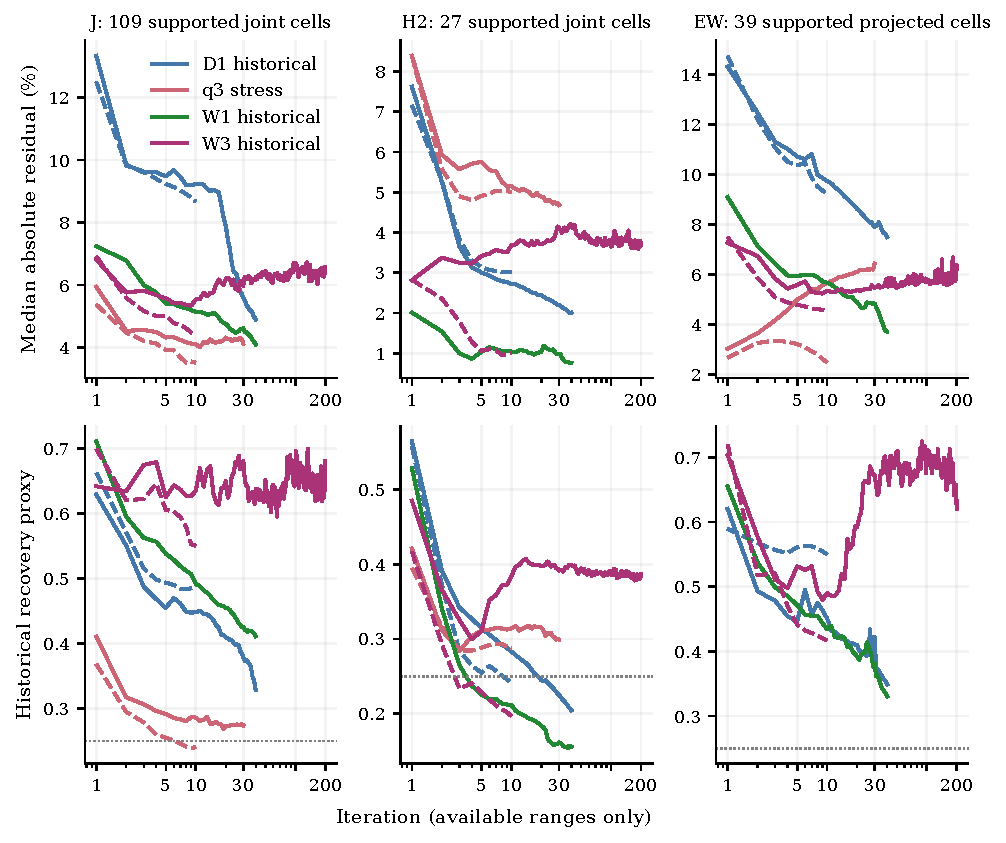
\includegraphics[width=\linewidth]{figures/gbdt_recovery.pdf}
\caption[Noise-free five-dimensional recovery against iterations]{In noise-free development traces, more iterations reduce the D1 and W1 residuals only slowly, and the W3 residual persists over the scan. Historical truth ratios, fixed simulated detector response. Solid/dashed OmniFold curves: 100 trees/8 leaves and 400/31. Iteration maxima: D1/W1 40, $q_3$ 30, W3 200, capacity probes 10. Some baseline traces end at their last saved checkpoint. Top: median $|\hat f/f_{\rm true}-1|$ over supported cells. Bottom: residual proxy $\operatorname{median}(|\hat f/f_{\rm true}-1|/|f_{\rm true}/f_0-1|)$ for departures above 1\%, dotted bound 0.25. Different denominators prevent reading one minus this proxy as an exact recovered fraction. The $q_3$ stress has no eligible EW departure. These traces measure no repeat variance.}
\label{fig:gbdt-recovery}
\end{figure}
% From sec_5d.tex:211 (draft 6ed12eed4)
At nominal truth, EW41 contains the truth in 15 of 40 68\% intervals (37.5\%, pointwise exact 95\% interval [22.7\%, 54.2\%]), so a pooled pass cannot qualify this cell. A check with the width averaged over several bootstrap estimates is in App.~\ref{app:devhistory}.
% From sec_5d.tex:225 (draft 6ed12eed4)
Twenty edge-safe data jitters (uniform input perturbations within half a single-precision unit in the last place that keep the fine-grid membership fixed) give a J-cell median SD of \SI{0.228}{\percent}, against a bootstrap SD of \SI{0.368}{\percent}.
% From sec_q3_fived16.tex:118 (draft 6ed12eed4)
At the two flagged truths, the root-mean-square bias of IBU at five iterations over the sixteen cells and its noise-free $\chi^2$ are \fvval{prr-cmp-gibuu} than configuration~(e)'s at the GiBUU hybrid truth and \fvval{prr-cmp-q3} at the $q_3$ tilt (Table~\ref{tab:fived16-prr}).
% From sec_q3_fived16.tex:120-134 (draft 6ed12eed4)
\begin{table}[htbp]
\centering\small
\caption[Retained prior at the two flagged truths]{At both flagged truths, IBU at five iterations overshoots the truth along the prior-to-truth direction, while configuration~(e) retains part of each departure. Retained fraction $\rho$, root-mean-square over the sixteen cells of the bias $b_c$, which is relative to the prior cross section, and noise-free $\chi^2$ (16 degrees of freedom) at the two flagged truths, for configuration~(e) and IBU at five iterations, on noise-free pseudo-data at one simulation split. A negative $\rho$ means that, along the prior-to-truth direction, the result overshoots the truth; the total bias is in the RMS and $\chi^2$ columns.}
\label{tab:fived16-prr}
\begin{tabular}{lcccccc}
\toprule
 & \multicolumn{2}{c}{$\rho$} & \multicolumn{2}{c}{RMS bias} & \multicolumn{2}{c}{$\chi^2$} \\
\cmidrule(lr){2-3}\cmidrule(lr){4-5}\cmidrule(lr){6-7}
truth & (e) & IBU & (e) & IBU & (e) & IBU \\
\midrule
GiBUU hybrid & $\fvval{prr-rho-e-gibuu}$ & $\fvval{prr-rho-ibu-gibuu}$ & \fvval{prr-rms-e-gibuu} & \fvval{prr-rms-ibu-gibuu} & \fvval{prr-chi2-e-gibuu} & \fvval{prr-chi2-ibu-gibuu} \\
$q_3$ tilt & $\fvval{prr-rho-e-q3}$ & $\fvval{prr-rho-ibu-q3}$ & \fvval{prr-rms-e-q3} & \fvval{prr-rms-ibu-q3} & \fvval{prr-chi2-e-q3} & \fvval{prr-chi2-ibu-q3} \\
\bottomrule
\end{tabular}
\end{table}
% From sec_q3_fived16.tex:138 (draft 6ed12eed4)
Reducing the iteration count from \fvval{prr-s53-b0-iters} to \fvval{prr-s53-k2-iters} increased $\rho$ beyond the threshold at the $q_3$ tilt. These settings [the reduced iteration count above, and the reduced capacity and $(\pT,\pPar)$-only learners of the note's \S\ref{sec:fived16-prr}] also newly flagged \fvval{prr-lev-K2-nnew}, \fvval{prr-lev-C25-nnew} and \fvval{prr-lev-O2-nnew} of the other \fvval{prr-lev-nother-word} graded truths, respectively, in the noise-free study. For \fvval{prr-pr1-noeffect}, no change as large as the threshold is detected. Every higher iteration count and capacity tested lowers $\rho$ at both truths, by at most \fvval{prr-more-dmax}, less than the threshold.

% [records reorg] former heading: \subsection{Five-dimensional estimator tests in full (from Part 5, P5-Q1)}
\paragraph{Five-dimensional estimator tests in full (from Part 5, P5-Q1).}
% DECISION-20261120a and the director's approved P5-Q plan (2026-11-20): the sentences of the note's sec_5d.tex that
% the condensed note no longer prints, moved verbatim and in order (rows CV-P5-Q1.* in
% history-cuts/move-manifest-cv-part5-20261119.tsv). The note's pointer: "supporting detail of these studies is in the records document".

% [records reorg] former heading: \paragraph{From the note's \S\ref{sec:5d}.}
\paragraph{From the note's \S\ref{sec:5d}.}
% From sec_5d.tex:5 (draft de1543818)
[The note's \S\ref{sec:5d}:] It covers what each test isolates (\S\ref{sec:val-fiveaxis}), background subtraction and generator-sized truth changes (\S\ref{sec:val-negweight}), why the estimator does not follow such changes (\S\ref{sec:val-departure}), model dependence and the reporting definitions it rules out (\S\ref{sec:gbdt-model-dependence}), the coverage test (\S\ref{sec:coverage-5d}) and the status of the five-axis covariance of the \resFiveAxis{} (the earlier note's section on the five-axis covariance; configurations in Table~\ref{tab:config-key}). The sixteen-cell result of the \estMultiD{} is given in \S\ref{sec:fived16}, and the calibrated generator tests built on a variant of this estimator in \S\ref{sec:joint5d}. The unbinned negative-weight background method itself is derived in App.~\ref{app:negweight}.

% [records reorg] former heading: \paragraph{From the note's \S\ref{sec:val-fiveaxis}.}
\paragraph{From the note's \S\ref{sec:val-fiveaxis}.}
% From sec_5d.tex:9 (draft de1543818)
Prior reweighting changes the frequencies of existing simulated truth events while retaining their detector-response simulation. A response mismatch instead changes how a given truth is reconstructed. Finite classifier capacity and iteration count approximate the inverse and can leave residuals in either case. Coverage asks whether the resulting intervals contain their specified target at the stated rate (\S\ref{sec:coverage-5d}). These mechanisms are separate: an incorrect generator prediction alone does not diagnose an interval failure. Each test below [in the note, \S\S\ref{sec:val-negweight}--the earlier note's section on the five-axis covariance] isolates one intervention.

\subsection{Closure tests and background-subtraction bias}\label{recsec:higherdim-closure}

% [records reorg] former heading: \subsubsection{From Part 4, the fake-data tests (row n63)}
\paragraph{From Part 4, the fake-data tests (row n63).}
% From sec_q3_fived16.tex:3 @e89694209; register row, check stage 2026-11-21
% absence-ok: verbatim move of a register sentence (a scoping statement of the test)
In the paragraph as the note printed it, this text followed: ``A truth is listed as failing when $p<\fvval{trig-p}$ or when any cell has $|z|>\fvval{trig-z}$ (pre-specified; Table~\ref{tab:test-index}).''\par
These are not held-out truths, and the detector response is not probed.

% [records reorg] former heading: \subsubsection{From Part 4, the fake-data control checks (row n65)}
\paragraph{From Part 4, the fake-data control checks (row n65).}
% From sec_q3_fived16.tex:47 @e89694209; register row, check stage 2026-11-21
In the paragraph as the note printed it, this text followed: ``The truths form three groups, evaluated separately, not pooled: the 8 truths from the $C_{\mathrm{model}}$ generators; the other truths, the GENIE CV hybrid and the $q_3$ tilt; and the prior truths, the simulation prior and the Tune~v1 hybrid.''\par
One control check failed: the offset check, which compares the offset corrections of two hybrid truths, gives $\chi^2=\fvval{f0b-control7-chi2}$ for 16 degrees of freedom. As fixed before any of the tests was graded, the six power alternatives built on that correction are therefore descriptive and not judged against the failure criteria; the records document gives them, with two descriptive variants of each tested truth (Ref.~\cite{NoteRecords2026}).

% [records reorg] former heading: \subsubsection{From Part 4, the per-cell validity rules}
\paragraph{From Part 4, the per-cell validity rules.}
% From sec_q3_fived16.tex:36 @e89694209; check-stage claims read
Three validity rules classify each cell from these tests; none is a coverage test, and no cell is excluded or changed by them. Under the ATLAS User Guide's thresholds applied per cell (V-ATLAS), \lrval{vr-atlas-nvalid} cells are valid, every cell except \lrval{vr-atlas-not}, where the GiBUU hybrid truth alone gives $z=\lrval{vr-R02-z-gibuu}$ and $\lrval{vr-R06-z-gibuu}$. The guide states no rule comparing the bias spread with the spread of the predictions, so the second rule (V-PRIOR) is ours: a cell is valid when the spread of its fake-data biases is below \lrval{vr-prior-tau} of the spread of the generator predictions. Under it \lrval{vr-prior-nvalid} cells are valid, every cell except \lrval{vr-prior-not}, and \lrval{vr-both-n} cells are valid under both rules. The third, the bias-half rule, asks that a cell's bias be at most half of the truth's departure from the prior, $|b_c|\leq0.5\,|d_c|$, with the bias $b_c$ and the departure $d_c$ both relative to the prior cross section (\S\ref{sec:fived16-prr}), at each graded truth where that departure is at least \SI{1}{\percent}. A cell is unresolved if its class changes within the noise of the estimate. The rule is a diagnostic that changes nothing in the reported result, and it was defined after the fake-data biases it classifies had been seen. Under it \fvval{vhalf-n-valid} cells pass, \fvval{vhalf-n-notvalid} fail (\fvval{vhalf-cells-notvalid}) and \fvval{vhalf-n-unresolved} are unresolved. V-ATLAS bounds the bias relative to the reported uncertainty and the bias-half rule bounds it relative to the truth's departure from the prior, so the two measure different properties of the bias.

% [records reorg] former heading: \subsubsection{From Part 4, the purity bias in standard deviations}
\paragraph{From Part 4, the purity bias in standard deviations.}
% From sec_5d.tex:23 @e89694209; check-stage claims read, second round
Relative to these cells' total uncertainty in the covariance of the \resFiveAxis{}, the bias is 0.36--1.07 standard deviations.

% [records reorg] former heading: \subsubsection{From Part 4, the low-capacity residual cells}
\paragraph{From Part 4, the low-capacity residual cells.}
% From sec_5d.tex:23 @e89694209; check-stage claims read, second round
Some joint cells remain up to \SI{1.0}{\percent} high, up to 14 standard errors, against \SI{-0.2}{\percent} without background. The mechanism is not established.

% [records reorg] former heading: \subsubsection{From Part 4, the purity bias and the widest mass bin}
\paragraph{From Part 4, the purity bias and the widest mass bin.}
% From sec_q3_negweight.tex:15 @e89694209; check-stage claims read, second round
Purity bias is 8--12 statistical standard deviations.

% [records reorg] former heading: \subsubsection{From Part 4, the retained fraction}
\paragraph{From Part 4, the retained fraction.}
% From sec_q3_fived16.tex:92 @e89694209; check-stage claims read, second round
The retained fraction is a directional summary and does not measure the total bias.

% Compression rewrite (DECISION-20261119c; REWRITE-RULES-20261119.md rule 5): text the cov2d lane moved verbatim out of
% the posted note's Part 5, with one move-manifest row per sentence (CV-P5 ids in
% history-cuts/move-manifest-cv-part5-20261119.tsv). References into the note resolve through main_note.aux (xr).
% [records reorg] former heading: \section{Validation detail moved from the note}
\paragraph{Validation detail moved from the note.}
This section holds supporting detail that the compressed note's Part 5 no longer prints, as the note printed it.

% [records reorg] former heading: \subsection{Closure detail (from Part 5, closures)}
\paragraph{Closure detail (from Part 5, closures).}
% From sec_q3_closure.tex:9 (draft lineage of 5d7210adc)
Both residuals are at least $30\times$ below the threshold: OmniFold recovers the injected truth shape.
% From sec_q3_3d.tex:5 (draft lineage of 5d7210adc)
Total normalization matches to better than \SI{1}{\percent}.
% From sec_q3_3d.tex:5 (draft lineage of 5d7210adc)
In the metric of \S\ref{sec:validation} ($\Eavail$ projection) the residual is \SI{1.84}{\percent} against \SI{18.1}{\percent} injected (ratio $0.102$).
% From sec_q3_3d.tex:8 (draft lineage of 5d7210adc)
The closure's marginal scatter is far below the $\SI{3.7}{\percent}$ data-versus-2D scatter.
% From sec_q3_3d.tex:8 (draft lineage of 5d7210adc)
The data comparison sets configuration (e) against configuration (f), a cross-configuration comparison.
% From sec_q3_3d.tex:8 (draft lineage of 5d7210adc)
That comparison's scatter is therefore not interpreted as data--simulation structure resolved by the available-energy axis, and the ratio of the two scatters is not quoted.
% From sec_q3_3d.tex:8 (draft lineage of 5d7210adc)
The hidden-variable closure exceeds its threshold at the largest amplitude (\S\ref{sec:validation}, the earlier note's appendix on the detector-response-mismatch closure).

% [records reorg] former heading: \paragraph{From the note's \S\ref{sec:val-negweight}.}
\paragraph{From the note's \S\ref{sec:val-negweight}.}
% From sec_5d.tex:24 (draft de1543818)
Without background, the same experiments [the note's end-to-end five-dimensional pseudo-experiments at nominal truth, here run without background events] recover the truth to \SI{0.22}{\percent}.
% From sec_5d.tex:34 (draft de1543818)
The \SI{74}{\percent} residual is in the cell $0.8\le\Eavail<\SI{1.5}{GeV}$, $W\ge\SI{3}{GeV}$, whose share of the cross section the deformation study did not record.
% From sec_5d.tex:43 (draft de1543818)
[For the \estMultiD{}'s recovered-fraction grade at the GiBUU-to-GENIE change and the three withheld shapes:] Its residual is the mean over 20 pseudo-experiments with backgrounds at each of these truths, each against its own half-sample truth. [At the GiBUU-to-GENIE change:] Of the \fvval{rec-g-n} supported cells with an injected change of magnitude above \SI{\fvval{rec-thr}}{\percent}, \fvval{rec-g-opp} move opposite to it and \fvval{rec-g-over} overshoot it. In the cell $0.8\le\Eavail<\SI{1.5}{GeV}$, $W\ge\SI{3}{GeV}$, the injected change is $\fvval{rec-g-ew29-inj}\,\%$, but the unfolded value lies \SI{\fvval{rec-g-ew29-unf}}{\percent} above the nominal truth.

% [records reorg] former heading: \subsection{Fake-data, closure and classifier detail (from Part 5, P5-Q2)}
\paragraph{Fake-data, closure and classifier detail (from Part 5, P5-Q2).}
% DECISION-20261120a and the director's approved P5-Q plan (2026-11-20): sentences of the note's sec_q3_fived16.tex,
% sec_q3_bias.tex and sec_q3_3d.tex that the condensed note no longer prints, moved verbatim and in order (rows
% CV-P5-Q2.* in history-cuts/move-manifest-cv-part5-20261119.tsv). Bracketed words are context, not the note's.

% [records reorg] former heading: \paragraph{From the note's \S\ref{sec:3d-closure}.}
\paragraph{From the note's \S\ref{sec:3d-closure}.}
% From sec_q3_bias.tex:21 (draft 16e2dfe7b)
[For the note's injected $\Eavail$ bump, unfolded with the \estPurity{}:] The recovered step-2 mean weight is $1.048$ against the injected $1.0485$. Residuals against reweighted truth on the $\Eavail$-marginal have median $0.9999$ and standard deviation \textbf{\num{0.0006}} (\SI{0.06}{\percent}).

% [records reorg] former heading: \paragraph{From the note's \S\ref{sec:fived16-fd}.}
\paragraph{From the note's \S\ref{sec:fived16-fd}.}
% From sec_q3_fived16.tex:33 (draft 16e2dfe7b)
[The listings of the note's fake-data tests use the reported construction of $C_{\mathrm{model}}$.] If $C_{\mathrm{model}}$ is built with GiBUU's ratio on the generators' common phase space, the listed truths are the same; this construction cannot change the grades of the two GiBUU truths, because their grading covariances omit GiBUU's component. If it is built from smoothed ratios, the NuWro hybrid truth is also listed, by its $p$ alone ($p=\fvval{rsn-sm-nuwro-p}$, no cell beyond $\fvval{trig-z}\sigma$). Under both constructions, the held-out tunes still meet both bias criteria.
% From sec_q3_fived16.tex:44 (draft 16e2dfe7b)
[Of the three groups of the note's fake-data truths, evaluated separately:] Under the reported covariance, the $C_{\mathrm{model}}$-generator truths have \fvval{f0b-grp-vertex-family-zcells} of \fvval{f0b-grp-vertex-family-cells} cells with $|z|>\fvval{trig-z}$ (Gaussian reference \fvval{f0b-grp-vertex-family-refcells}) and \fvval{f0b-grp-vertex-family-ptruths} of \fvval{f0b-grp-vertex-family-truths} truths with $p<\fvval{trig-p}$ (reference \fvval{f0b-grp-vertex-family-reftruths}); the other truths \fvval{f0b-grp-non-vertex-zcells} of \fvval{f0b-grp-non-vertex-cells} and \fvval{f0b-grp-non-vertex-ptruths} of \fvval{f0b-grp-non-vertex-truths}; and the prior truths \fvval{f0b-grp-prior-zcells} of \fvval{f0b-grp-prior-cells} and \fvval{f0b-grp-prior-ptruths} of \fvval{f0b-grp-prior-truths}. The Gaussian references are context only, because the bias is deterministic.

\subsection{Prior dependence and algorithmic robustness}\label{recsec:higherdim-prior}

% [records reorg] former heading: \subsection{From App. A, appstatmethodsnd.tex: the paragraph beginning ``The synthesis in Srefsec:gbdt-model-dependence reuses saved''}
\paragraph{From App. A, appstatmethodsnd.tex: the paragraph beginning ``The synthesis in Srefsec:gbdt-model-dependence reuses saved''.}
% From app_statmethods_nd.tex:25 @d55f7aad6; qualifier detail or procedure (DECISION-20261120a, second pass)
The synthesis in \S\ref{sec:gbdt-model-dependence} reuses saved outputs. It involves no new unfolding, training or pseudo-experiments.

% [records reorg] former heading: \subsection{From App. A, appstatmethodsnd.tex: the paragraph beginning ``The synthesis in Srefsec:gbdt-model-dependence reuses saved''}
\paragraph{From App. A, appstatmethodsnd.tex: the paragraph beginning ``The synthesis in Srefsec:gbdt-model-dependence reuses saved''.}
% From app_statmethods_nd.tex:25 @d55f7aad6; qualifier detail or procedure (DECISION-20261120a, second pass)
In the paragraph as the note printed it, this text followed: ``The saved trace functionals on the EW cells are differential in $(\Eavail,W)$ and are multiplied by the cell areas. Those on the J and H2 cells are already integrals.''\par
Direct tensor-slice integration checks the index-map sums and full-domain rate. Reporting boundaries coincide with fine edges.

% [records reorg] former heading: \subsubsection{From Part 4, unfolding-model dependence at the withheld shapes}
\paragraph{From Part 4, unfolding-model dependence at the withheld shapes.}
% From sec_5d.tex:88 @e89694209; check-stage claims read
For historical shapes held out while this candidate was assessed (NuWro; GENIE with enhanced meson-exchange currents), its unfolding-model dependence is median \SIrange{2}{6}{\percent} and at most \SIrange{16}{31}{\percent}, within the total uncertainty of the \resFiveAxis{} in 20 of the 42 $(\Eavail,W)$ cells. No uncertainty from this assessment is used for a quoted result.

% [records reorg] former heading: \subsubsection{From Part 4, the held-out GENIE~v3 tunes}
\paragraph{From Part 4, the held-out GENIE~v3 tunes.}
% From sec_q3_fived16.tex:54 @e89694209; check-stage claims read (Grok, sec. 4 finding 5)
In the paragraph as the note printed it, this text followed: ``The bias meets both criteria in all four records, the pseudo-experiment mean and the closure at each tune.''\par
Both are GENIE tunes, so they are partial evidence and not independent tests.

% [records reorg] former heading: \subsubsection{From Part 4, the generator-sized change}
\paragraph{From Part 4, the generator-sized change.}
% From sec_5d.tex:52 @e89694209; check-stage claims read, second round
In the paragraph as the note printed it, this text followed: ``With noise-free pseudo-data, thirty iterations reduce the $\Eavail$ residual by \SI{26}{\percent}. The $\Eavail$ residual continues to fall slowly, while the $q_3$ residual grows with iterations.''\par
No single cause is established, and no estimator change within the scope of the study meets the recovery requirement (pre-specified; Table~\ref{tab:test-index}) for the GiBUU-to-GENIE departure.

% [records reorg] former heading: \subsubsection{From Part 4, the binned IBU comparison on data}
\paragraph{From Part 4, the binned IBU comparison on data.}
% From sec_q3_fived16.tex:100 @e89694209; check-stage claims read, second round
A reading of differ means that a difference is detectable at this noise; it does not show that either method is correct.

% [records reorg] former heading: \subsubsection{From Part 4, the held-out tunes, cell R11}
\paragraph{From Part 4, the held-out tunes, cell R11.}
% From sec_q3_fived16.tex:52 @e89694209; check-stage claims read, second round
In the paragraph as the note printed it, this text followed: ``In every cell of the four records, the bias is below \fvval{f1-bsig-ceil} of the cell's reported $\sigma$;''\par
in cell R11 at \fvval{f1-tune-g18}, the bias lies below the reported uncertainty only with $C_{\mathrm{model}}$ included.

% [records reorg] former heading: \subsection{Fake-data and unfolding-algorithm detail (from Part 5, P5-4a)}
\paragraph{Fake-data and unfolding-algorithm detail (from Part 5, P5-4a).}
% The director's approved P5-4 plan (2026-11-19): procedure and descriptive detail behind Part 5's fake-data and IBU
% findings, moved verbatim (rows CV-P5-4a.* in history-cuts/move-manifest-cv-part5-20261119.tsv).
% From sec_q3_fived16.tex:36 (draft 190331a95)
The methods paper withholds this second rule's counts [V-PRIOR, the note's \S\ref{sec:fived16-fd}], because its generator spread uses the CH-corrected NuWro and GiBUU predictions (\S\ref{sec:joint5d-ch}). The counts remain the recorded classification.
% From sec_q3_fived16.tex:44 (draft 190331a95)
A descriptive comparison made after the grades, against smaller matrices, finds the biases, apart from the listed truths, small next to the reported covariance and, apart from the two closures at the prior, large next to its statistical block alone. It changes no grade.
% From sec_q3_fived16.tex:47 (draft 190331a95)
The other eight control checks [besides the failed offset check, the note's \S\ref{sec:fived16-fd}] passed.
% From sec_q3_fived16.tex:49-72 (draft 190331a95)
\begin{table}[htbp]
\centering\footnotesize
\caption[Descriptive fake-data numbers]{Descriptive fake-data numbers only, without test outcomes. In-sample: reported $C_{\mathrm{total}}+C_{\mathrm{resp}}+C_{\mathrm{PL,5D}}$, including the truth's generator shift, supplies no evidence (--- where the test already uses the full matrix). Model-only: statistical block plus $C_{\mathrm{model}}$ without that shift, omitting interaction, flux, detector, lateral and normalization blocks, gives a lower bound on $C_{\mathrm{model}}$'s reach. Power alternatives on Tune~v1 (r) and GENIE CV (g): NuWro $(\pT,\pPar,\Eavail)$ shape (P1), NuWro $q_3$ shape at fixed $(\Eavail,W)$ (P2), GENIE + MEC $(\Eavail,W)$ shape (P3).}
\label{tab:fived16-fdvar}
\scriptsize\setlength{\tabcolsep}{3pt}
\begin{tabular}{@{}lrrr@{\qquad}lrrr@{}}
\toprule
truth & \multicolumn{2}{c}{in-sample $\chi^2$, $p$} & model-only $\chi^2$ & power alternative & $n$ & $\chi^2$ & $p$ \\
\midrule
simulation prior (MINERvA Tune~v1) & --- & --- & \fvval{f0b-nominal-model_only-chi2} & P1r & \fvval{f0b-P1r-n} & \fvval{f0b-P1r-chi2} & $\fvval{f0b-P1r-p}$ \\
MINERvA Tune~v1, hybrid & --- & --- & \fvval{f0b-A7_mnvtune-model_only-chi2} & P2r & \fvval{f0b-P2r-n} & \fvval{f0b-P2r-chi2} & $\fvval{f0b-P2r-p}$ \\
GENIE CV, hybrid & --- & --- & \fvval{f0b-A7_genie_cv-model_only-chi2} & P3r & \fvval{f0b-P3r-n} & \fvval{f0b-P3r-chi2} & $\fvval{f0b-P3r-p}$ \\
GENIE + MEC, hybrid & \fvval{f0b-A7_genie_mec-in_sample-chi2} & $\fvval{f0b-A7_genie_mec-in_sample-p}$ & \fvval{f0b-A7_genie_mec-model_only-chi2} & P1g & \fvval{f0b-P1g-n} & \fvval{f0b-P1g-chi2} & $\fvval{f0b-P1g-p}$ \\
GENIE + MEC, $(\Eavail,W)$ shape (W2) & \fvval{f0b-W2-in_sample-chi2} & $\fvval{f0b-W2-in_sample-p}$ & \fvval{f0b-W2-model_only-chi2} & P2g & \fvval{f0b-P2g-n} & \fvval{f0b-P2g-chi2} & $\fvval{f0b-P2g-p}$ \\
NuWro, hybrid & \fvval{f0b-A7_nuwro-in_sample-chi2} & $\fvval{f0b-A7_nuwro-in_sample-p}$ & \fvval{f0b-A7_nuwro-model_only-chi2} & P3g & \fvval{f0b-P3g-n} & \fvval{f0b-P3g-chi2} & $\fvval{f0b-P3g-p}$ \\
NuWro, $\Eavail$ shape (W1) & \fvval{f0b-W1-in_sample-chi2} & $\fvval{f0b-W1-in_sample-p}$ & \fvval{f0b-W1-model_only-chi2} & & & & \\
NuWro, $(\pT,\pPar,\Eavail)$ shape (W3) & \fvval{f0b-W3-in_sample-chi2} & $\fvval{f0b-W3-in_sample-p}$ & \fvval{f0b-W3-model_only-chi2} & & & & \\
NuWro, closure (noise-free) & \fvval{f0b-closure_nuwro-in_sample-chi2} & $\fvval{f0b-closure_nuwro-in_sample-p}$ & \fvval{f0b-closure_nuwro-model_only-chi2} & & & & \\
GiBUU, $\Eavail$ shape & \fvval{f0b-stage0c_gibuu-in_sample-chi2} & $\fvval{f0b-stage0c_gibuu-in_sample-p}$ & \fvval{f0b-stage0c_gibuu-model_only-chi2} & & & & \\
GiBUU, hybrid & \fvval{f0b-A7_gibuu-in_sample-chi2} & $\fvval{f0b-A7_gibuu-in_sample-p}$ & \fvval{f0b-A7_gibuu-model_only-chi2} & & & & \\
synthetic $q_3$ tilt & --- & --- & \fvval{f0b-q3-model_only-chi2} & & & & \\
\bottomrule
\end{tabular}
\end{table}
% From sec_q3_fived16.tex:75 (draft 190331a95)
Each tune enters as its normalized shape ratio to GENIE CV on the fine grid, constructed as the reweighting ratios of the $C_{\mathrm{model}}$ shifts are. Where the tune's sample fails the ratio's statistical gate, the ratio is pooled over a coarser cell or set to one. The ratio is applied to the simulated truth, under the simulation's detector response.
% From sec_q3_fived16.tex:77 (draft 190331a95)
The mean of the pseudo-experiments gives $\chi^2=\fvval{f1-g18-chi2}$ ($p=\fvval{f1-g18-p}$; largest $|z|$ \fvval{f1-g18-zmax}, in \fvval{f1-g18-zcell}) at \fvval{f1-tune-g18} and \fvval{f1-ar23-chi2} ($p=\fvval{f1-ar23-p}$; \fvval{f1-ar23-zmax}, in \fvval{f1-ar23-zcell}) at \fvval{f1-tune-ar23}; the closures give \fvval{f1-closure-g18-chi2} ($p=\fvval{f1-closure-g18-p}$; \fvval{f1-closure-g18-zmax}, in \fvval{f1-closure-g18-zcell}) and \fvval{f1-closure-ar23-chi2} ($p=\fvval{f1-closure-ar23-p}$; \fvval{f1-closure-ar23-zmax}, in \fvval{f1-closure-ar23-zcell}). This group has \fvval{f1-grp-zcells} of \fvval{f1-grp-cells} cells with $|z|>\fvval{trig-z}$ (Gaussian reference \fvval{f1-grp-refcells}) and \fvval{f1-grp-ptruths} of \fvval{f1-grp-truths} records with $p<\fvval{trig-p}$ (reference \fvval{f1-grp-reftruths}). The four records are the pseudo-experiment and closure results for two truths, so the Gaussian references, which count them as independent, are context only.
% From sec_q3_fived16.tex:79 (draft 190331a95)
The two tunes use the same quasielastic cross-section model, GENIE's \texttt{NievesQELCCPXSec}, \fvval{f1-tune-ar23} with a z-expansion form factor, and the MEC model of \fvval{f1-tune-g18} is of the Valencia family used in the GENIE + MEC shift. Descriptively, without the GENIE + MEC shift, the pseudo-experiments give $\chi^2=\fvval{f1-g18-sens-chi2}$ ($p=\fvval{f1-g18-sens-p}$) and \fvval{f1-ar23-sens-chi2} ($p=\fvval{f1-ar23-sens-p}$), and the closures \fvval{f1-closure-g18-sens-chi2} ($p=\fvval{f1-closure-g18-sens-p}$) and \fvval{f1-closure-ar23-sens-chi2} ($p=\fvval{f1-closure-ar23-sens-p}$). The model-only $\chi^2$, defined as in Table~\ref{tab:fived16-fdvar}, are \fvval{f1-mo-chi2-min}--\fvval{f1-mo-chi2-max} in the four records, with cell \fvval{f1-ar23-mo-cells} beyond $\fvval{trig-z}\sigma$ at \fvval{f1-tune-ar23} in both its records. Rerunning the tests with the two tunes added reproduces every earlier fake-data result exactly.
% From sec_q3_fived16.tex:128 (draft 190331a95)
Descriptively, at a NuWro closure the IBU's median absolute residual is \lrval{rg1-r2-nuwro} times that of configuration~(e), and at the simulation's own truth, a trivial closure, the IBU's residual vanishes; neither is a coverage statement for either estimator.

% [records reorg] former heading: \paragraph{From the note's \S\ref{sec:val-departure}.}
\paragraph{From the note's \S\ref{sec:val-departure}.}
% From sec_5d.tex:51 (draft de1543818)
With noise-free pseudo-data the unfolding recovers more than \SI{99}{\percent} of the change that the departure produces in the reconstructed distribution, whereas the median $(\Eavail,W)$ truth residual ranges from \SI{5}{\percent} to \SI{11}{\percent}, with \SI{74}{\percent} in the worst cell. The unrecovered reconstructed-level difference is small relative to the departure but statistically significant at the analysis exposure.
% From sec_5d.tex:53 (draft de1543818)
A larger classifier improves the reconstructed-level fit without reducing the $\Eavail$ truth residual, and removing the regression for events that fail reconstruction does not reduce that residual either.
% From sec_5d.tex:60 (draft de1543818)
[In the comparison with exact binned unfolding:] At five iterations the J-cell medians of the absolute residual agree: \SI{9.5}{\percent}, \SI{5.4}{\percent}, \SI{5.6}{\percent} and \SI{4.3}{\percent} for the boosted trees, against \SI{8.3}{\percent}, \SI{5.4}{\percent}, \SI{4.9}{\percent} and \SI{5.3}{\percent} for the exact binned unfolding, for D1, W1, W3 and the $q_3$ stress.
% From sec_5d.tex:71 (draft de1543818)
The instability [the \estMultiD{}'s data-stability failure under rounding-level input changes] also explains the difference of at most \SI{1.2}{\percent} on data between the driver and the development pipeline.
% From sec_5d.tex:78 (draft de1543818)
[The ensemble-averaged variant of the \estMultiD{} fails its no-worse closure requirement only at the GiBUU $\Eavail$ shape.] There, on noise-free fake data, its root-mean-square closure bias is \fvval{ens1-g-rms-r} against \fvval{ens1-g-rmsc-r} for the \estMultiD{}, about \fvval{ens1-g-rms-dpct}\,\% larger. The excess is \fvval{ens1-g-drms} against a noise floor of \fvval{ens1-g-floor}, or \fvval{ens1-g-ratio} times the floor. In noise-free fake-data closures at the other \fvval{ens1-nnoworse} of the \fvval{ens1-ntruths} distinct truths, it is no worse than the \estMultiD{}. On the sixteen cells of the data (\S\ref{sec:fived16}), the ensemble average differs from the reported result by at most \SI{\fvval{e96d-maxpct}}{\percent}, and by at most \fvval{e96d-maxsig} of a cell's standard deviation from $C_{\mathrm{e}}$ (\S\ref{sec:fived16-cov}). Its fits perturb a float64 copy of the inputs at the rounding level. On the unperturbed copy, the \estMultiD{} gives the reported result to double precision.

% [records reorg] former heading: \paragraph{From the note's \S\ref{sec:gbdt-model-dependence}.}
\paragraph{From the note's \S\ref{sec:gbdt-model-dependence}.}
% From sec_5d.tex:99 (draft de1543818)
[Estimator $R$:] With seed 42, its 40 nominal experiments and 20 at each of five departures include Poisson pseudo-data, changing MC splits and background refinement.
% From sec_5d.tex:136 (draft de1543818)
The selection procedure then takes RD3 as the fallback, and RD3 fails the total-width target.
% From sec_5d.tex:149 (draft de1543818)
At historical W3 truth, EW29 has mean residual \SI{23.67}{\percent} and repeat SD \SI{0.56}{\percent}; EW7 has \SI{-6.81}{\percent} and \SI{0.30}{\percent}. Coarser cells can have smaller residuals and spread, but they estimate different integrals, so their smaller residuals and spread are not an improvement in precision on an unchanged quantity.
% From sec_5d.tex:155 (draft de1543818)
[Caption of the note's Fig.~\ref{fig:gbdt-bias-spread}, continued:] Each supported J or H2 cell gives the mean and SD of $(\hat f-f_{\rm true})/f_{\rm true}$ in the same background-inclusive ensemble: 40 nominal experiments, 20 each for W2 and W3. Bars give pointwise 95\% Student-$t$ intervals for means and normal-model intervals for SDs, conditional on saved simulation. They supply neither simultaneous bounds nor total uncertainties. Truth panels and reporting cells form no frontier across estimator settings.
% From sec_5d.tex:168 (draft de1543818)
[Caption of the note's the earlier note's GBDT coverage figure, continued:] Below: EW7 ($\Eavail\in[0.1,0.2)$, $W\in[1.1,1.4)$ GeV) and EW41 (both above 3 GeV), pointwise 95\% Clopper--Pearson bounds. Dotted: nominal Gaussian 68.27\%. Neither total uncertainty nor a newly validated interval is shown. The bootstrap $\sigma$ is from 100 replicas of the nominal seed 700000; the assessment samples are reused, and no per-experiment or total-coverage claim is made.
% From sec_5d.tex:184 (draft de1543818)
[Caption of the note's Fig.~\ref{fig:gbdt-prior}, continued:] Historical W3 at five iterations. Horizontal gives minus the noise-free relative truth residual; vertical gives the relative shift in real-data $R$ when its MC prior changes to W3, normalized to CV-prior results. Points are supported cells, not independent repeated experiments. The diagonal marks equality.

% [records reorg] former heading: \paragraph{From the note's \S\ref{sec:fived16-ibu}.}
\paragraph{From the note's \S\ref{sec:fived16-ibu}.}
% From sec_q3_fived16.tex:100 (draft 16e2dfe7b)
[Between the note's sixteen cells and the binned IBU unfolding of the same data:] The largest differences, IBU minus the \estMultiD{} as fractions of the \estMultiD{}, are $\fvval{ibu16-dof-R11}\,\%$ in R11, $\fvval{ibu16-dof-R06}\,\%$ in R06 and $\fvval{ibu16-dof-R05}\,\%$ in R05, or \fvval{ibu16-dsig-R11}, \fvval{ibu16-dsig-R06} and \fvval{ibu16-dsig-R05} times each cell's reported standard deviation; over the sixteen cells the difference reaches \fvval{ibu16-dsig-max} times a cell's reported standard deviation.
% From sec_q3_fived16.tex:103 (draft 16e2dfe7b)
[In the same comparison:] The IBU uncertainty is a median \lrval{rg1-r3-med} times that of the \estMultiD{} over the sixteen cells (\lrval{rg1-r3-lo}--\lrval{rg1-r3-hi}); the \estMultiD{}'s statistical block includes its estimator's own noise, refit per replica, and the IBU has none.

% [records reorg] former heading: \paragraph{From the note's \S\ref{sec:3d-classifier}.}
\paragraph{From the note's \S\ref{sec:3d-classifier}.}
% From sec_q3_3d.tex:9 (draft 16e2dfe7b)
[Caption of the note's Fig.~\ref{fig:calibration}, continued:] The five-iteration OmniFold cross-check uses identical weighted 3D inputs and extraction, changing only the classifier family. The MLP/GBDT total-cross-section ratio is $1.0078$; median absolute projection differences are \SI{1.20}{\percent} in $\pT$, \SI{1.36}{\percent} in $\pPar$, and \SI{0.66}{\percent} in $\Eavail$.

\subsection{Uncertainty calibration and the scope of the five-axis covariance}\label{recsec:higherdim-calibration}

% [records reorg] former heading: \subsubsection{From Part 4, the five-axis covariance's acceptance}
\paragraph{From Part 4, the five-axis covariance's acceptance.}
% From sec_5d.tex:230 @e89694209; check-stage claims read, second round
The five-axis covariance used in this note does not meet the acceptance criteria of its specification: its metadata mark it as not passing and as not to be used, and the null bound that the specification requires to be fixed before production was not fixed for it.

% [records reorg] former heading: \subsubsection{From Part 4, the scope of the five-axis covariance's use}
\paragraph{From Part 4, the scope of the five-axis covariance's use.}
% From sec_5d.tex:230 @e89694209; check-stage claims read, second round
The use does not extend to any other covariance built to the same specification, including the two companion covariances of the measurements below.

% [records reorg] former heading: \subsubsection{From Part 4, the diagonal seed measures}
\paragraph{From Part 4, the diagonal seed measures.}
% From sec_5d.tex:270 @e89694209; check-stage claims read, second round
Two other measures read the diagonal only: $s_{\mathrm{agg}}$, the maximum relative change in $\sqrt{\mathrm{Tr}\,C}$, and $s_{\mathrm{med}}$, the maximum relative change in the median of the per-bin relative standard deviations. Both pass ($s_{\mathrm{agg}}=\saggMeasured\,\%$, $s_{\mathrm{med}}=\smedMeasured\,\%$).

% [records reorg] former heading: \paragraph{From the note's \S\ref{sec:coverage-5d}.}
\paragraph{From the note's \S\ref{sec:coverage-5d}.}
% From sec_5d.tex:215 (draft de1543818)
[Caption of the note's Fig.~\ref{fig:coverage-5d-paper}, continued:] Circles/squares: 68\%/95\% intervals. Bars: one-sided Clopper--Pearson lower/upper bounds at level $0.05/459$ (Bonferroni: 153 integrals, three truths). Solid/dashed: nominal coverage/thresholds 0.66 and 0.94. Filled: upper bound below threshold. Nominal truth (undrawn): none below 0.66, two below 0.94. Order: 42 $(\Eavail,W)$ cells and sum, \jtNcells{} joint cells (indices in $3^5$), total.

% [records reorg] former heading: \paragraph{From the note's the earlier note's section on the five-axis covariance.}
\paragraph{From the note's the earlier note's section on the five-axis covariance.}
% From sec_5d.tex:271 (draft de1543818)
A 160-throw ensemble determines a standard deviation only to a relative precision of about $1/\sqrt{2(N-1)}\approx\SI{5.6}{\percent}$ for independent Gaussian throws, so a smaller seed-induced drift could not be resolved against the width it would change.
% From sec_5d.tex:274 (draft de1543818)
[Item 2 of the note's list of what the covariance supports:] Within the limits stated below, the sensitivity is not the statistic's own resampling noise, which would fall with $N$. The same-seed resampling floor falls steeply from $\floorNforty\,\%$ at $N=40$ to $\floorNeighty\,\%$ at $N=80$, with two-point exponent $\floorExponent$; no floor measurement exists at $N=160$. Three limits rule out a statement about infinite ensembles. First, the $40$- and $80$-throw points are nested subsets of the same 160 throws, not independent ensembles. The flatness [of the seed sensitivity over the 40-, 80- and 160-throw ensembles, stated in the note] therefore holds within one ensemble, over a factor of four in $N$; the behavior at larger $N$ is unmeasured. Second, the scatter of these subset means, $\pm\seedEffectScatter\,\%$, is at a single seed pair (offsets $\{0,1200\}$); the width of the distribution over seed pairs is unmeasured. Third, the statistic is a maximum over the specified offset set, so additional pairs can only raise it.
% Search: floor at N=160; larger ensemble; seed-pair width; seed pairs (values.tex:446 "the FLOOR was measured at N=40 and N=80 ONLY"; nd-unfolding/CORRECTED_UQ_PRODUCTION_STATUS.md:17-22, the 40- and 80-throw points nested in one 160-throw ensemble at one seed pair; CORRECTION-20260921-seed-effect-larger-ensemble-corollary-withdrawn.md:71-74, the N=160 floor of EVIDENCE-20260920 is an extrapolation; release-package-20260922/README.md:35-39, larger N and the seed-pair width unmeasured) @ 624acea1 [carried from sec_5d.tex:275]
% From sec_5d.tex:276 (draft de1543818)
[Of the five bands that fall outside the seed variation (item 3):] Allowing them to vary could move the total in either direction, and neither is measured, because $s_{\mathrm{proj}}$ maximizes relative changes over functionals rather than summing nonnegative component contributions.
% From sec_5d.tex:277 (draft de1543818)
[Item 4:] Individual five-axis bins reach $\cvMoveBinOverSigmaMax\,\%$ of their uncertainty; summing bins suppresses this movement in projections.

\subsection{Figure and table detail}\label{recsec:higherdim-captions}

% [records reorg] former heading: \subsection{Caption detail (caption pass, Part 4)}
\paragraph{Caption detail (caption pass, Part 4).}
% The director's ruling of 2026-11-20 (option (a)): secondary caption sentences of Part 4, moved verbatim (rows
% CV-CAP4.* in history-cuts/move-manifest-cv-captions-20261120.tsv). Bracketed words are context, not the note's.
% From sec_fived16_gen.tex:112 (draft d55f7aad6)
[Caption of the note's Fig.~\ref{fig:fived16-modes}, continued:] Predictions use analysis definitions.
% From sec_fived16_gen.tex:177 (draft d55f7aad6)
[Caption of the note's the earlier note's table of the generator distances' dependence on $C_{\mathrm{model}}$, continued:] The CH column is this note's sensitivity, omitted by the methods paper because it uses the free-proton samples of \S\ref{sec:joint5d-ch}.
% From sec_3d.tex:93 (draft d55f7aad6)
[Caption of the note's Fig.~\ref{fig:eavail-marg}, continued:] See the \estPurity{} definition in the method configurations (\S\ref{sec:method-config}).
% From sec_3d.tex:132 (draft d55f7aad6)
[Caption of the note's Fig.~\ref{fig:3dmodels}, continued:] The fourth-axis comparison (\S\ref{sec:4d}) gives $\Eavail$-marginal data/Tune~v1 ratios.
% From sec_3d.tex:170 (draft d55f7aad6)
[Caption of the note's Fig.~\ref{fig:modedecomp}, continued:] The remainder of the gap [the low-$\Eavail$ data$-$CV gap left after GENIE regenerated with Valencia 2p2h closes about half of it, in central values] occupies the region the MINERvA tune's empirical enhancement is built to absorb.
% From sec_3d.tex:202 (draft d55f7aad6)
[Caption of the note's Fig.~\ref{fig:q3excess}, continued:] See the \estPurity{} method definition (\S\ref{sec:method-config}).


% Restored 2026-11-21 (check stage, journal-editor): the journal-voice rewrite dropped sec_fps.tex from the note (SECTION-PLAN.md,
% "Leaving the paper (-> records document)"), and no records file input it, so its register rows n76 and n77 had no home.
% The file is input whole and unchanged; the note's pointer is sec6_conclusions.tex ("Related exploratory studies, of an
% extended fiducial region, ... are documented in the analysis records").
% [records reorg] former heading: \subsection{The extended fiducial phase-space study, formerly in the note}
\subsection{The extended fiducial phase-space study, formerly in the note}
This section was a subsection of the analysis note until its journal-voice rewrite of 21 November 2026, which moved it here unchanged; in it, ``this section'' means the study below.
% [records reorg] former heading, merged into the records' R4.8 heading (Joseph, 2026-11-21, flag b): \subsection{Extended fiducial phase-space study (preliminary; no reported covariance)}
\label{sec:fps}

% Cutdown 2026-11-16 (DECISION-20261116-joseph-paper-batch.md item 33; history-cuts/sec_fps.md): the section is one paragraph, built from the base's own sentences. The value stays with its caveats: it was produced with the binned purity correction, its control does not reproduce the quoted two-dimensional result, and its NuWro-shaped prior was not rebuilt after the flux repair. The acceptance description, the validation-test list, the reporting-grid paragraph and the three figures are cut; their text stays at 8342963c1:sec_fps.tex.
The preliminary extended-fiducial CC-inclusive central value on the tracker fiducial volume is $\sigma_{\mathrm{ext}} = \SI{\fpsSigma}{cm^2/nucleon}$, compared with $\SI{\sigTwoDPurity}{cm^2/nucleon}$ for the control unfolding in the restricted phase space. This scalar central value has a three-prior dependence envelope. The total cross section varies by $\pm\SI{1.5}{\percent}$ across three priors (MINERvA Tune~v1, bare GENIE and NuWro-shaped).

The signal remains $\nu_\mu$ CC in the tracker interaction fiducial volume. The truth-muon kinematic cuts are removed, but the reconstructed MINOS-based selection is unchanged. The domain is an extended \emph{fiducial} one. Unrestricted neutrino phase space is outside it. In regions without acceptance the unfolding extrapolates through the step-1 regressor for missed events.

The extended-fiducial central value was produced with the binned purity correction. Its production did not use refined negative-weight subtraction. That subtraction is the treatment designated for the extended-fiducial analysis (App.~\ref{app:negweight}). The control unfolds the standard 2D input on the published binning, with settings identical to the extended-domain unfolding's. The control's total, $\SI{\sigTwoDPurity}{cm^2/nucleon}$, agrees at the printed precision with the purity-subtracted 2D totals (exact-split and LightGBM). The quoted 2D result, which uses refined negative-weight subtraction, is $\SI{\sigTwoD}{cm^2/nucleon}$, \SI{\roFpsDiff}{\percent} lower, so the control does not reproduce it.

The NuWro-shaped prior reweights the truth $(\pT,\pPar)$ shape to two million raw NuWro events without phase-space cuts. The sample's mis-sampled flux (App.~\ref{app:devhistory-3d}) suppresses its high-$\pPar$ shape, and this prior was not rebuilt after the flux repair.

We adopt \textbf{two-tier reporting}. \emph{Tier~1} comprises the acceptance-supported cells (reconstruction efficiency $\epsilon\gtrsim2\%$): the published region and the measurable part of the extension, which carries $\sim\SI{6}{\percent}$ of the rate, chiefly in the $\theta>20^{\circ}$ wedge and the $\pPar\in[0.75,1.5]\,\si{GeV/c}$ edge. \emph{Tier~2}, prior-extrapolated, comprises the low-acceptance cells ($\sim\SI{28}{\percent}$ of the rate) and is flagged separately with an explicit additional three-prior envelope band. Both tiers enter the sum. Both shares are rate fractions. Neither is a separate cross section. Only tier~1 is the acceptance-supported part of this scalar central value.

Neither tier is a completed measurement. The three-prior envelope gives the spread of the three central values. It supplies no coverage interval. Tier~1 has no qualified uncertainty. No uncertainty magnitude is assigned beyond the three-prior envelope, because no extended-domain covariance has been constructed with re-selected lateral bands, whose procedure is described in the records document.

% Source comments of the section as it stood at 8342963c1, kept for provenance (they cite the sources of sentences above and of sentences now cut):
% Accuracy fix (unscored; Joseph, DECISION-20261026-joseph-fps-scope-r04-sensitivity-and-tex-reflow.md, via the director 2026-10-26): "No corrected covariance exists for it" was
% false as read: an extended-fiducial covariance with re-selected lateral bands exists (job 56431823, 2026-08-07;
% nd-unfolding/uq_fps/corrected/FPS_UQ_CORRECTED_STATE.md:127) but is not quoted (AGENTS.md:36).
% Search: extended-fiducial covariance quoted; corrected FPS covariance; activelat (note, paper and primer closures: no
% printed extended-fiducial covariance or uncertainty beyond the three-prior envelope; AGENTS.md:36 "Old unified 4D/FPS
% covariances ... are unquotable") @ 7ad668f4
% Register pass b8 (2026-10-22): register only; every number and limitation kept (ledger.md rows F*).
% RE-2 integration W3 (approved, DECISION-20261024-joseph-approve-integration-wording-s1-compute-preserve.md): RE2-PARTC-REPORT.md sec. 8 (RO-FPS: E_R 3.069e-38 against the control's 3.073e-38, -0.14 %,
% "It does not reproduce"); the control: VALIDATION_LEDGER.md:1624-1625 (no committed digest; VL177 records the -0.14 %); the exact-split total
% 3.0733e-38 (values.tex \sigTwoD comment).
        % \texttt{KNOWN\_ISSUES.md} row 83; flux repair of 2026-09-27
% absence-ok: "is not tested" is the containment diagnostic's own scope statement, reworded in r22 Step 2
% RE-2 integration W5 (approved, DECISION-20261024-joseph-approve-integration-wording-s1-compute-preserve.md): \fpsAbove (46) is not printed; its definition is not established (RE2-PARTC-REPORT.md sec. 4: 4.502/3.0730 - 1 = 46.50 %; VALIDATION_LEDGER.md:1626 "+46% vs restricted" names no operand). The two totals: VALIDATION_LEDGER.md:1624-1625 (control 3.073e-38; FPS total 4.502e-38).
% Accuracy fix (unscored; Joseph, DECISION-20261026-joseph-fps-scope-r04-sensitivity-and-tex-reflow.md, via the director 2026-10-26): "No extended-fiducial production with
% refined negative-weight subtraction has been run" was false as read: ten negweight-refined extended-fiducial endpoint
% unfolds were run later (job 56430128; nd-unfolding/sbatch_unfold_active_fps.sh:18,34-35,60). The sentence now says
% only what the quoted central value used, in the words of Joseph's selected option, and keeps the base sentence's fact that a
% negative-weight treatment is designated for this analysis. That treatment is refined negative-weight subtraction: App. C
% sec:negweight-footing designates negative-weight injection with Stay-Positive refinement (app_negweight.tex:148), the
% refined form of negative-weight injection (:105) whose refinement is the Stay-Positive classifier (:180) (director, 2026-10-26; line numbers updated in n3 for App. C's adopted text, director ruling (c)).
% Search: extended-fiducial central value; fps battery; 54244120; negweight-refined FPS central value (app_provenance.tex
% fps-battery; no refined extended-fiducial central value is recorded; sbatch_unfold_active_fps.sh:67 takes the existing
% central value as input) @ 7ad668f4
% Search: extended-domain covariance with re-selected lateral bands; activelat; 56431823; sec:uq-combine procedure (true as scoped, Joseph's ruling DECISION-20261026-joseph-fps-scope-r04-sensitivity-and-tex-reflow.md item 1.3: the activelat FPS covariance of job 56431823, AUDIT-FINDINGS-20260820-fps.md:217-221, was built on 2026-08-07, before the sec:uq-combine procedure with C_PL was adopted on 2026-10-17, DECISION-20261017-joseph-2d-adopt-s5-plus-playlist.md, and is unquotable, AGENTS.md:36, AUDIT-FINDINGS-20260820-fps.md:389-390) @ 0d9c64fd
% The former subsection "Recoil-PET feasibility study on the extended population"
% (label sec:fps-pet) moved to sec_pet.tex, sec:pet-full-event-status (lane 3 §10.1).


\section{The sixteen-cell cross section}\label{recsec:sixteen}
% Generated by records_reorg.py assemble (records-reorg/); edit the data and re-run, not this file.
\subsection{Cells, covariance blocks and the uncertainty budget}\label{recsec:sixteen-budget}

\paragraph{The sixteen-cell run-period block.} The first is one existing component, within two standard deviations of its own size, explaining at least half of both period-group patterns. The second is a replica spread of the block's median per-cell width above half that width. The third is, in the median replica, less than half of the replica-built block's variance lying in the observed block's plane.
% [records reorg] former heading: \subsubsection{The sixteen-cell run-period block}

\paragraph{Quadrant comparisons with the 2D result.} In the note, the first and second comparisons are the two quadrant tests that follow this paragraph (\S\ref{sec:fived16-quadrants}).\par On the sixteen-cell side the covariance is the reported one; on the two-dimensional side it is the four-block covariance of \S\ref{sec:uq-combine} in the first comparison below, and that covariance with its generator-shape term $C_{\mathrm{model}}$ in the second. The two results share the data, the flux and most systematic variations, and come from different estimators: the \estMultiD{} for the sixteen cells and the \estTwoD{} for the two-dimensional result (\S\ref{sec:method-config}, Table~\ref{tab:config-key}). The three-observable marginal of the \estMultiD{}, compared with the two-dimensional result over all 205 reported cells, agrees with it to \SI{0.141}{\percent} in area-weighted total (\S\ref{sec:3d-anchor}); that is a different quantity from the quadrant differences below, of which QA's is $\fvval{cr-QA-dpct}$\,\%. The sixteen cells form four $(\pT,\pPar)$ quadrants, divided at $\pT=\fvval{h2-mid-pt}$ and $\pPar=\fvval{h2-mid-pz}$~GeV/$c$, of four cells each.
% [records reorg] former heading: \subsection{From Part 4, secfived16.tex: the paragraph beginning ``The sixteen cells form four (pT,pPar)''}
% From sec_fived16.tex:56 @0d1f8208a; qualifier detail or procedure (DECISION-20261120a)
% [lead-in, Option B] In the paragraph as the note printed it, this text followed: ``In each quadrant the sum $S_{16}$ of the sixteen-cell result is compared with the sum $S_{\mathrm{2D}}$ of the adopted two-dimensional result over the same region, through $d=S_{16}-S_{\mathrm{2D}}$.''\par
% [records reorg] former heading: \subsection{From Part 4, secfived16.tex: the paragraph beginning ``The sixteen cells form four (pT,pPar)''}
% From sec_fived16.tex:56 @0d1f8208a; qualifier detail or procedure (DECISION-20261120a)
% [records reorg] former heading: \subsection{From Part 4, secfived16.tex: the paragraph beginning ``The sixteen cells form four (pT,pPar)''}
% From sec_fived16.tex:56 @0d1f8208a; qualifier detail or procedure (DECISION-20261120a)
% [records reorg] former heading: \subsection{From Part 4, secfived16.tex: the paragraph beginning ``The sixteen cells form four (pT,pPar)''}
% From sec_fived16.tex:56 @c1f74f696; qualifier detail or procedure (DECISION-20261120a, second pass)

\paragraph{Event-loop modes for lateral bands.} Two event-loop modes supply the lateral bands. The single-pass event loop, which writes every universe in one pass, stores each lateral universe's shifted observables only for events that pass the selection at the central value, so it omits events that the shift moves into the selection. Re-selected event loops re-run the selection with one lateral universe active at a time, so they include these migrations.
% [records reorg] former heading: \subsection{From Part 4, secfived16.tex: the paragraph beginning ``Two event-loop modes supply the lateral''}
% From sec_fived16.tex:113 @0d1f8208a; qualifier detail or procedure (DECISION-20261120a)
% [records reorg] former heading: \subsection{From Part 4, secfived16.tex: the paragraph beginning ``Two event-loop modes supply the lateral''}
% From sec_fived16.tex:113 @0d1f8208a; qualifier detail or procedure (DECISION-20261120a)
% [records reorg] former heading: \subsection{From Part 4, secfived16.tex: the paragraph beginning ``Two event-loop modes supply the lateral''}
% From sec_fived16.tex:113 @0d1f8208a; qualifier detail or procedure (DECISION-20261120a)

\paragraph{Bands outside the kinematic replacement.} MINOS efficiency and the three GEANT hadron-interaction bands (GEANT\_Neutron, GEANT\_Pion, GEANT\_Proton) keep their weight-based treatment and are therefore outside the kinematic replacement. This classification does not independently validate hadronic-response model completeness for the $\Eavail$ and $W$ results.
% [records reorg] former heading: \subsection{From Part 4, secfived16.tex: the paragraph beginning ``The replacement covers the five detector''}
% From sec_fived16.tex:117 @0d1f8208a; qualifier detail or procedure (DECISION-20261120a)
% [records reorg] former heading: \subsection{From Part 4, secfived16.tex: the paragraph beginning ``The replacement covers the five detector''}
% From sec_fived16.tex:117 @0d1f8208a; qualifier detail or procedure (DECISION-20261120a)

\paragraph{Scope of $C_Z$.} The 4D and extended-fiducial results have no covariance from this procedure, and $C_Z$ is not transferred to them.
% [records reorg] former heading: \subsection{From Part 4, secfived16.tex: the paragraph beginning ``Subtracting the background separately in each''}
% From sec_fived16.tex:119 @0d1f8208a; qualifier detail or procedure (DECISION-20261120a)
% [lead-in, Option B] In the paragraph as the note printed it, this text followed: ``Subtracting the background separately in each of the 187 universe unfolds and in the CV changes the square-root trace of the combined block sum by \SI{0.28}{\percent} and $C_Z$ by \SI{0.18}{\percent}, a numerically negligible bound on the background-CV choice (Ref.~\cite{NoteRecords2026}, superseded values).''\par

\paragraph{Components of $C_{\mathrm{e}}$.} $C_{\mathrm{e}}$ sums the statistical bootstrap of the \estMultiD{}, 50 replicas, each of which refits the whole unfolding with its own rounding-level perturbation of the inputs; the PPFX flux universes, weighted by the neutrino--electron and inverse-muon-decay constraint; the interaction-model and detector bands, which reweight simulated events; the lateral bands, which shift reconstructed kinematics (\S\ref{sec:systematics}); the normalization; and the training-seed block. With full-sample binning and deterministic training, the unfolds at the other seeds are bitwise equal to the central one, so the measured training-seed block is zero in every cell. Table~\ref{tab:fived16-groups} gives each group's per-cell relative $\sigma$.
% [records reorg] former heading: \subsection{From Part 4, secfived16.tex: the paragraph beginning ``The reported covariance is Cmathrmtotal+Cmathrmresp+CmathrmPL,5D, with''}
% From sec_fived16.tex:125 @0d1f8208a; qualifier detail or procedure (DECISION-20261120a)
% [lead-in, Option B] In the paragraph as the note printed it, this text followed: ``The reported covariance is $C_{\mathrm{total}}+C_{\mathrm{resp}}+C_{\mathrm{PL,5D}}$, with $C_{\mathrm{total}}=C_{\mathrm{e}}+C_{\mathrm{model}}$ (each block is defined in Table~\ref{tab:definitions}); the run-period block $C_{\mathrm{PL,5D}}$ is described in \S\ref{sec:fived16-pl}.''\par
% [records reorg] former heading: \subsection{From Part 4, secfived16.tex: the paragraph beginning ``The reported covariance is Cmathrmtotal+Cmathrmresp+CmathrmPL,5D, with''}
% From sec_fived16.tex:125 @0d1f8208a; qualifier detail or procedure (DECISION-20261120a)
% [records reorg] former heading: \subsection{From Part 4, secfived16.tex: the paragraph beginning ``The reported covariance is Cmathrmtotal+Cmathrmresp+CmathrmPL,5D, with''}
% From sec_fived16.tex:125 @0d1f8208a; qualifier detail or procedure (DECISION-20261120a)

\paragraph{Generator-shape block $C_{\mathrm{model}}$.} In the paragraph as the note printed it, this text followed: ``For $C_{\mathrm{model}}$, the prior is reweighted in turn by the ratio of GENIE + MEC, NuWro or GiBUU to GENIE CV, and the data are unfolded again.''\par Each generator's shift is the relative change of the data result. Their unscaled outer-product sum is the fractional covariance $C_{\mathrm{model}}^{\mathrm{frac}}$. In cross-section units the block is $C_{\mathrm{model}}=\mathrm{diag}(x)\,C_{\mathrm{model}}^{\mathrm{frac}}\,\mathrm{diag}(x)$, with $x$ the cell-integrated cross sections on the reporting cells. In the paragraph as the note printed it, this text followed: ``It measures generator-shape model dependence.''\par Its status as an uncertainty is stated in \S\ref{rlim:fived16}. For $C_{\mathrm{model}}$, the prior is reweighted in turn by the ratio of GENIE + MEC, NuWro or GiBUU to GENIE CV, and the data are unfolded again. It measures generator-shape model dependence.
% [records reorg] former heading: \subsection{From Part 4, secfived16.tex: the paragraph beginning ``For Cmathrmmodel, the prior is reweighted''}
% From sec_fived16.tex:128 @0d1f8208a; qualifier detail or procedure (DECISION-20261120a)
% [records reorg] former heading: \subsection{From Part 4, secfived16.tex: the paragraph beginning ``For Cmathrmmodel, the prior is reweighted''}
% From sec_fived16.tex:128 @0d1f8208a; qualifier detail or procedure (DECISION-20261120a)
% [records reorg] former heading: \subsection{From Part 4, secfived16.tex: the paragraph beginning ``For Cmathrmmodel, the prior is reweighted''}
% From sec_fived16.tex:128 @0d1f8208a; qualifier detail or procedure (DECISION-20261120a)
% [records reorg] former heading: \subsection{From Part 4, secfived16.tex: the paragraph beginning ``For Cmathrmmodel, the prior is reweighted''}
% From sec_fived16.tex:128 @0d1f8208a; qualifier detail or procedure (DECISION-20261120a)
% [records reorg] former heading: \subsection{From Part 4, secfived16.tex: the paragraph beginning ``For Cmathrmmodel, the prior is reweighted''}
% From sec_fived16.tex:128 @c1f74f696; qualifier detail or procedure (DECISION-20261120a, second pass)
% carried with the text from sec_fived16.tex:129 @c1f74f696
% Search: coverage of C_model at held-out truths; validated intervals of the sixteen-cell result (nd-unfolding/pv-ladder/readouts/cmodel_5d.json labels.coverage: "coverage at held-out truths was not validated (DECISION-20261024-joseph-5d-community-standard-route.md item 3); the paper states this as a limitation"; FD-F0b-REPORT.md NOT CITABLE FOR coverage) @ 8b0f83fd

\paragraph{GiBUU reweighting and $C_{\mathrm{model}}$ trace.} Between $\pPar=\fvval{cmodel-gibuu-pz-lack}$ and \fvval{cmodel-gibuu-pz-max}~GeV/$c$, the GiBUU sample lacks the contribution from $E_\nu>\fvval{cmodel-gibuu-enu}$~GeV, which is at least \fvval{cmodel-gibuu-lack-lo}--\fvval{cmodel-gibuu-lack-hi}\% of the cross section there in the GENIE CV and NuWro samples (which stop at $E_\nu=\fvval{gagg-range-max}$~GeV). The GiBUU shift contributes \fvval{cmodel-trace-gibuu} of the trace of $C_{\mathrm{model}}^{\mathrm{frac}}$, the NuWro shift \fvval{cmodel-trace-nuwro} and the GENIE + MEC shift \fvval{cmodel-trace-genie_mec}. In every cell, \fvval{cmodel-step-lo}--\fvval{cmodel-step-hi}\% of the prior weight lies next to a discontinuity larger than \fvval{cmodel-step-r} in the reweighting ratio, created by the ratio's statistical gate or by a cut; the shifts are used unmodified. The GiBUU reweighting is applied only below $\pPar=\fvval{cmodel-gibuu-pz-max}$~GeV/$c$; above it the prior is unchanged.
% [records reorg] former heading: \subsection{From Part 4, secfived16.tex: the paragraph beginning ``The GiBUU reweighting is applied only''}
% From sec_fived16.tex:131 @0d1f8208a; qualifier detail or procedure (DECISION-20261120a)
% [lead-in, Option B] In the paragraph as the note printed it, this text followed: ``The GiBUU reweighting is applied only below $\pPar=\fvval{cmodel-gibuu-pz-max}$~GeV/$c$; above it the prior is unchanged.''\par
% [records reorg] former heading: \subsection{From Part 4, secfived16.tex: the paragraph beginning ``The GiBUU reweighting is applied only''}
% From sec_fived16.tex:131 @0d1f8208a; qualifier detail or procedure (DECISION-20261120a)
% [records reorg] former heading: \subsection{From Part 4, secfived16.tex: the paragraph beginning ``The GiBUU reweighting is applied only''}
% From sec_fived16.tex:131 @0d1f8208a; qualifier detail or procedure (DECISION-20261120a)
% [records reorg] former heading: \subsection{From Part 4, secfived16.tex: the paragraph beginning ``The GiBUU reweighting is applied only''}
% From sec_fived16.tex:131 @c1f74f696; qualifier detail or procedure (DECISION-20261120a, second pass)
% carried with the text from sec_fived16.tex:132 @c1f74f696
% Search: coverage of C_model at held-out truths; validated intervals of the sixteen-cell result (nd-unfolding/pv-ladder/readouts/cmodel_5d.json labels.coverage: "coverage at held-out truths was not validated (DECISION-20261024-joseph-5d-community-standard-route.md item 3); the paper states this as a limitation"; FD-F0b-REPORT.md NOT CITABLE FOR coverage) @ 8b0f83fd

\paragraph{Run-period block $C_{\mathrm{PL,5D}}$.} As for the two-dimensional result (\S\ref{sec:uq-combine}, Table~\ref{tab:pl-added}), the block $C_{\mathrm{PL,5D}}$ is built from these double ratios with no reference period. With $e_X$ the exposure share of period group $X$, $r_X$ that group's unfolded result over its own simulated truth, and $m=\sum_X e_X r_X$, the fractional offset is $g_X=r_X/m-1$. The reliability-weight factor is $k=V_2/(1-V_2)$, where $V_2=\sum_X e_X^2$. The block is $k\sum_X e_X (x\circ g_X)(x\circ g_X)^{T}$, with $x$ the central value on these cells. It has rank \fvval{pl-rank} and is not debiased for the replica noise it contains. With three groups its own size is poorly determined. The period offsets are treated as exchangeable draws with a common variance. The 68\,\% interval on the ratio of its true to its estimated $\sigma$, \fvval{pl-sigratio-lo}--\fvval{pl-sigratio-hi}, is the interval of a chi-squared distribution with the Satterthwaite degrees of freedom of this exposure-weighted spread. It depends only on the exposure shares. It is not a coverage or calibration of the block. The offsets of the twelve playlists differ between the three period groups by more than expected from their playlist-to-playlist scatter. The cells in which the block is dominated by the replica noise it contains are named in \S\ref{rlim:fived16}.
% [records reorg] former heading: \subsection{From Part 4, secfived16.tex: the paragraph beginning ``On the sixteen cells, the unfolded''}
% From sec_fived16.tex:208 @0d1f8208a; qualifier detail or procedure (DECISION-20261120a)
% [lead-in, Option B] In the paragraph as the note printed it, this text followed: ``The cause is not known, and these data cannot establish which period, if any, is right.''\par
% [records reorg] former heading: \subsection{From Part 4, secfived16.tex: the paragraph beginning ``On the sixteen cells, the unfolded''}
% From sec_fived16.tex:208 @0d1f8208a; qualifier detail or procedure (DECISION-20261120a)
% [records reorg] former heading: \subsection{From Part 4, secfived16.tex: the paragraph beginning ``On the sixteen cells, the unfolded''}
% From sec_fived16.tex:208 @0d1f8208a; qualifier detail or procedure (DECISION-20261120a)
% [records reorg] former heading: \subsection{From Part 4, secfived16.tex: the paragraph beginning ``On the sixteen cells, the unfolded''}
% From sec_fived16.tex:208 @0d1f8208a; qualifier detail or procedure (DECISION-20261120a)
% [records reorg] former heading: \subsection{From Part 4, secfived16.tex: the paragraph beginning ``On the sixteen cells, the unfolded''}
% From sec_fived16.tex:208 @0d1f8208a; qualifier detail or procedure (DECISION-20261120a)
% [records reorg] former heading: \subsection{From Part 4, secfived16.tex: the paragraph beginning ``On the sixteen cells, the unfolded''}
% From sec_fived16.tex:208 @0d1f8208a; qualifier detail or procedure (DECISION-20261120a)
% [records reorg] former heading: \subsection{From Part 4, secfived16.tex: the paragraph beginning ``On the sixteen cells, the unfolded''}
% From sec_fived16.tex:208 @0d1f8208a; qualifier detail or procedure (DECISION-20261120a)
% [records reorg] former heading: \subsection{From Part 4, secfived16.tex: the paragraph beginning ``On the sixteen cells, the unfolded''}
% From sec_fived16.tex:208 @0d1f8208a; qualifier detail or procedure (DECISION-20261120a)
% [records reorg] former heading: \subsection{From Part 4, secfived16.tex: the paragraph beginning ``On the sixteen cells, the unfolded''}
% From sec_fived16.tex:208 @0d1f8208a; qualifier detail or procedure (DECISION-20261120a)
% [records reorg] former heading: \subsection{From Part 4, secfived16.tex: the paragraph beginning ``On the sixteen cells, the unfolded''}
% From sec_fived16.tex:208 @0d1f8208a; qualifier detail or procedure (DECISION-20261120a)
% [records reorg] former heading: \subsection{From Part 4, secfived16.tex: the paragraph beginning ``On the sixteen cells, the unfolded''}
% From sec_fived16.tex:208 @c1f74f696; qualifier detail or procedure (DECISION-20261120a, second pass)
% [lead-in, Option B] In the paragraph as the note printed it, this text followed: ``On the sixteen cells, the unfolded results of the three run-period groups (playlists 1A--1F, 1G--1M and 1N--1P), each over its own simulated truth (the double ratio), differ from one another by more than the scatter of their bootstrap replicas.''\par
% [records reorg] former heading: \subsection{From Part 4, secfived16.tex: the paragraph beginning ``The cells in which the block''}
% From sec_fived16.tex:210 @0d1f8208a; qualifier detail or procedure (DECISION-20261120a)

\paragraph{Single-playlist unfoldings.} Each of the twelve playlists was also unfolded on its own, with its own simulation and bootstrap replicas, in a study whose tests, bounds and readings were fixed before any playlist result was read. A playlist's offset is its double ratio on the sixteen cells relative to the exposure-weighted mean of the twelve. In each of \fvval{rpd-datasets} simulated datasets the playlists' offsets are drawn independently from one covariance, estimated from the twelve playlists and scaled by 0, 0.5, 1 or 2, with each playlist's own bootstrap and simulation noise added; the share of datasets with $p<0.05$ is \fvval{rpd-alpha-lo}--\fvval{rpd-alpha-hi} over the four scales, within the bound of \fvval{rpd-alpha-gate}. For an alternative chronological division into groups of five, two, two and three playlists (1A--1E, 1F and 1G, 1L and 1M, and 1N--1P), the same statistic gives $p=\fvval{rpd-pera}$ over its \fvval{rpd-npart-era} divisions; this comparison is descriptive.
% [records reorg] former heading: \subsection{From Part 4, secfived16.tex: the paragraph beginning ``Each of the twelve playlists was''}
% From sec_fived16.tex:212 @0d1f8208a; qualifier detail or procedure (DECISION-20261120a)
% [records reorg] former heading: \subsection{From Part 4, secfived16.tex: the paragraph beginning ``Each of the twelve playlists was''}
% From sec_fived16.tex:212 @0d1f8208a; qualifier detail or procedure (DECISION-20261120a)
% [records reorg] former heading: \subsection{From Part 4, secfived16.tex: the paragraph beginning ``Each of the twelve playlists was''}
% From sec_fived16.tex:212 @0d1f8208a; qualifier detail or procedure (DECISION-20261120a)
% [lead-in, Option B] In the paragraph as the note printed it, this text followed: ``The permutation is approximate: the playlists differ in exposure and hence in noise, so their labels are not exchangeable, and the test's validity rests on a simulated null.''\par
% [records reorg] former heading: \subsection{From Part 4, secfived16.tex: the paragraph beginning ``Each of the twelve playlists was''}
% From sec_fived16.tex:212 @0d1f8208a; qualifier detail or procedure (DECISION-20261120a)

\paragraph{Location of the run-period step.} To locate the step, each playlist's own step was measured against 1A--1F, leaving the playlist out when it is one of them. A step consistent with none within two standard deviations is classed FREE. A step larger than half of the 1G--1M group's step, recombined from its three playlists, by two standard deviations is classed CARRIES. A step that is neither is classed PARTIAL (Fig.~\ref{fig:runperiod-steps}(b)). The classes are CARRIES for \fvval{rpd-r1-carries}; PARTIAL for \fvval{rpd-r1-partial}; and FREE for \fvval{rpd-r1-free}. The study's two patterns are that all three of 1G, 1L and 1M carry the step, or that some carry it and the others are free, each with 1A--1F free. Neither holds, so no statement of where the step lies is drawn from these classes. None of these readings identifies a cause.
% [records reorg] former heading: \subsection{From Part 4, secfived16.tex: the paragraph beginning ``In the form of the two-dimensional''}
% From sec_fived16.tex:214 @0d1f8208a; qualifier detail or procedure (DECISION-20261120a)
% [lead-in, Option B] In the paragraph as the note printed it, this text followed: ``In the form of the two-dimensional test (\S\ref{sec:uq-combine}), the five-observable unfolds of the run-period groups give the double ratio of 1G--1M to 1A--1F a $\pPar$ step of $(\fvval{rpd-s0}\pm\fvval{rpd-s0-sigma})\,\%$ across \SI{8}{GeV/c}, $\fvval{rpd-s0-z}$ times its bootstrap scatter.''\par
% [records reorg] former heading: \subsection{From Part 4, secfived16.tex: the paragraph beginning ``In the form of the two-dimensional''}
% From sec_fived16.tex:214 @0d1f8208a; qualifier detail or procedure (DECISION-20261120a)
% [records reorg] former heading: \subsection{From Part 4, secfived16.tex: the paragraph beginning ``In the form of the two-dimensional''}
% From sec_fived16.tex:214 @0d1f8208a; qualifier detail or procedure (DECISION-20261120a)
% [records reorg] former heading: \subsection{From Part 4, secfived16.tex: the paragraph beginning ``In the form of the two-dimensional''}
% From sec_fived16.tex:214 @0d1f8208a; qualifier detail or procedure (DECISION-20261120a)
% [records reorg] former heading: \subsection{From Part 4, secfived16.tex: the paragraph beginning ``In the form of the two-dimensional''}
% From sec_fived16.tex:214 @0d1f8208a; qualifier detail or procedure (DECISION-20261120a)
% [records reorg] former heading: \subsection{From Part 4, secfived16.tex: the paragraph beginning ``In the form of the two-dimensional''}
% From sec_fived16.tex:214 @0d1f8208a; qualifier detail or procedure (DECISION-20261120a)
% [records reorg] former heading: \subsection{From Part 4, secfived16.tex: the paragraph beginning ``In the form of the two-dimensional''}
% From sec_fived16.tex:214 @0d1f8208a; qualifier detail or procedure (DECISION-20261120a)
% [records reorg] former heading: \subsection{From Part 4, secfived16.tex: the paragraph beginning ``In the form of the two-dimensional''}
% From sec_fived16.tex:214 @0d1f8208a; qualifier detail or procedure (DECISION-20261120a)

\paragraph{Effect of adding the run-period block.} The median of the cells' own increases is \fvval{pl-cellrise-med}\,\%, and the largest is \fvval{pl-cellrise-max}\,\%, in \fvval{pl-cellrise-maxcell}. The block's median per-cell relative $\sigma$ is \fvval{sigmed-C_PL5D}\,\%, at most \fvval{sigmax-C_PL5D}\,\%, and its share of the reported variance has a median of \fvval{pl-share-med}\,\% over the cells and a maximum of \fvval{pl-share-max}\,\%. We infer from these falls that the predictions' residuals have components along the directions the rank-\fvval{pl-rank} block adds; the comparison does not test this interpretation. Under the reported covariance one fake-data truth fewer is listed (\S\ref{sec:fived16-fd}), with the bias unchanged. With the block, each prediction's total $\chi^2$ is lower by \fvval{pl-chi2fall-total-lo}--\fvval{pl-chi2fall-total-hi}\,\% of its value without it, and each shape-only $\chi^2$ by \fvval{pl-chi2fall-shape_only-lo}--\fvval{pl-chi2fall-shape_only-hi}\,\%, for the five predictions with NuWro and GiBUU corrected to CH (Tables~\ref{tab:fived16-gen} and~\ref{tab:fived16-gen-target}).
% [records reorg] former heading: \subsection{From Part 4, secfived16.tex: the paragraph beginning ``Added to Cmathrmtotal+Cmathrmresp, the block raises''}
% From sec_fived16.tex:233 @0d1f8208a; qualifier detail or procedure (DECISION-20261120a)
% [lead-in, Option B] In the paragraph as the note printed it, this text followed: ``Added to $C_{\mathrm{total}}+C_{\mathrm{resp}}$, the block raises the median per-cell relative $\sigma$ from \fvval{sigmed-C_total_resp}\,\% to \fvval{sigmed-reported}\,\%, by about \fvval{pl-medrise}\,\%.''\par
% [records reorg] former heading: \subsection{From Part 4, secfived16.tex: the paragraph beginning ``Added to Cmathrmtotal+Cmathrmresp, the block raises''}
% From sec_fived16.tex:233 @0d1f8208a; qualifier detail or procedure (DECISION-20261120a)
% [records reorg] former heading: \subsection{From Part 4, secfived16.tex: the paragraph beginning ``Added to Cmathrmtotal+Cmathrmresp, the block raises''}
% From sec_fived16.tex:233 @0d1f8208a; qualifier detail or procedure (DECISION-20261120a)
% [lead-in, Option B] In the paragraph as the note printed it, this text followed: ``With the block, each prediction's total $\chi^2$ is lower by \fvval{pl-chi2fall-total-lo}--\fvval{pl-chi2fall-total-hi}\,\% of its value without it, and each shape-only $\chi^2$ by \fvval{pl-chi2fall-shape_only-lo}--\fvval{pl-chi2fall-shape_only-hi}\,\%, for the five predictions with NuWro and GiBUU corrected to CH (Tables~\ref{tab:fived16-gen} and~\ref{tab:fived16-gen-target}).''\par
% [records reorg] former heading: \subsection{From Part 4, secfived16.tex: the paragraph beginning ``Added to Cmathrmtotal+Cmathrmresp, the block raises''}
% From sec_fived16.tex:233 @0d1f8208a; qualifier detail or procedure (DECISION-20261120a)
% [records reorg] former heading: \subsection{From Part 4, secfived16.tex: the paragraph beginning ``Added to Cmathrmtotal+Cmathrmresp, the block raises''}
% From sec_fived16.tex:233 @c1f74f696; qualifier detail or procedure (DECISION-20261120a, second pass)
% [lead-in, Option B] In the paragraph as the note printed it, this text followed: ``Added to $C_{\mathrm{total}}+C_{\mathrm{resp}}$, the block raises the median per-cell relative $\sigma$ from \fvval{sigmed-C_total_resp}\,\% to \fvval{sigmed-reported}\,\%, by about \fvval{pl-medrise}\,\%.''\par

\paragraph{Contents of the sixteen-cell section.} Statements in those sections about that central value and that covariance do not describe this result, and statements here do not describe them. The section gives the cells and the result (\S\ref{sec:fived16-result}), the result's quadrant sums against the lower-dimensional results (\S\ref{sec:fived16-quadrants}), the covariance and what it is built from (\S\ref{sec:fived16-cov}), the fake-data tests of the estimator's bias against the covariance (\S\ref{sec:fived16-fd}), the dependence on the unfolding algorithm (\S\ref{sec:fived16-ibu}) and the descriptive comparison with generator predictions (\S\ref{sec:fived16-gen}).
% [records reorg] former heading: \subsection{From Part 4, secfived16.tex: the paragraph beginning ``This section gives the five-dimensional output''}
% From sec_fived16.tex:5 @7686f6ae7; qualifier detail or procedure (DECISION-20261120a)
% [lead-in, Option B] In the paragraph as the note printed it, this text followed: ``This section gives the five-dimensional output of the \estMultiD{} (\S\ref{sec:method-config}) on the data, on 16 cells, R00--R15, with total uncertainties from the reported covariance $C_{\mathrm{total}}+C_{\mathrm{resp}}+C_{\mathrm{PL,5D}}$. It is illustrative output, not for fitting or for constraining models: no interval has validated coverage, the fake-data bias exceeds the stated criteria at \fvval{f0b-nlisted} truths (\S\ref{sec:fived16-fd}), the cells \fvval{h2-lowstab-cells} have low reconstruction stability (\S\ref{sec:fived16-result}), the run-period block was added after the period differences were seen (\S\ref{sec:fived16-pl}), and the cells depend on the unfolding algorithm (\S\ref{sec:fived16-ibu}). It is a separate product from the five-dimensional central value of the \estPurity{}, the \resFiveAxis{}, of Secs.~\ref{sec:eavailw} and~\ref{sec:5d} and from the five-axis covariance used with that central value (\S\ref{sec:eavailw-adopted}).''\par

\paragraph{Formation of the sixteen cells.} Of these, \fvval{h2-nsupported} meet that appendix's support rule (minimum expected signal and truth weight). Each supported box with purity below $\tau=\fvval{h2-tau}$ is merged into a neighbor, in \fvval{h2-nmerge} predefined steps. The merges absorb \fvval{h2-nabsorbed} unsupported box into cell R09; the other \fvval{h2-nunreported} are not reported. No stability criterion is applied in forming the cells. The cells are formed from the H2 grid of \S\ref{sec:gbdt-model-dependence}, which divides each axis once into \fvval{h2-nboxes} boxes, with edges $\pT=(\fvval{h2-edges-pt})$, $\pPar=(\fvval{h2-edges-pz})$, $\Eavail=(\fvval{h2-edges-eavail})$, $q_3=(\fvval{h2-edges-q3})$ and $W=(\fvval{h2-edges-W})$, in the units of App.~\ref{sec:gbdt-diagnostic-definitions}. Each of the 16 resulting cells meets the support rule. Four of them, \fvval{h2-lowstab-cells}, have a reconstruction stability of \fvval{h2-lowstab-min}--\fvval{h2-lowstab-max} (the other twelve, \fvval{h2-stab-rest-min}--\fvval{h2-stab-rest-max}): of the simulated signal events generated in such a cell and reconstructed, that fraction is reconstructed in the same cell.
% [records reorg] former heading: \subsection{From Part 4, secfived16.tex: the paragraph beginning ``The cells are formed from the''}
% From sec_fived16.tex:9 @7686f6ae7; qualifier detail or procedure (DECISION-20261120a)
% [lead-in, Option B] In the paragraph as the note printed it, this text followed: ``The cells are formed from the H2 grid of \S\ref{sec:gbdt-model-dependence}, which divides each axis once into \fvval{h2-nboxes} boxes, with edges $\pT=(\fvval{h2-edges-pt})$, $\pPar=(\fvval{h2-edges-pz})$, $\Eavail=(\fvval{h2-edges-eavail})$, $q_3=(\fvval{h2-edges-q3})$ and $W=(\fvval{h2-edges-W})$, in the units of App.~\ref{sec:gbdt-diagnostic-definitions}.''\par
% [records reorg] former heading: \subsection{From Part 4, secfived16.tex: the paragraph beginning ``The cells are formed from the''}
% From sec_fived16.tex:9 @7686f6ae7; qualifier detail or procedure (DECISION-20261120a)
% [lead-in, Option B] In the paragraph as the note printed it, this text followed: ``Four of them, \fvval{h2-lowstab-cells}, have a reconstruction stability of \fvval{h2-lowstab-min}--\fvval{h2-lowstab-max} (the other twelve, \fvval{h2-stab-rest-min}--\fvval{h2-stab-rest-max}): of the simulated signal events generated in such a cell and reconstructed, that fraction is reconstructed in the same cell.''\par
% [records reorg] former heading: \subsection{From Part 4, secfived16.tex: the paragraph beginning ``The cells are formed from the''}
% From sec_fived16.tex:9 @c1f74f696; qualifier detail or procedure (DECISION-20261120a, second pass)

\paragraph{Unreported boxes in quadrant sums.} The two quadrants with $\pT<\fvval{h2-mid-pt}$~GeV/$c$ include unreported boxes at their central value, a share of at most $\fvval{g3d-qa-unrep}$ of the sum.
% [records reorg] former heading: \subsection{From Part 4, secfived16.tex: the paragraph beginning ``Summed over each of the four''}
% From sec_fived16.tex:107 @7686f6ae7; qualifier detail or procedure (DECISION-20261120a)
% [lead-in, Option B] In the paragraph as the note printed it, this text followed: ``Summed over each of the four $(\pT,\pPar)$ quadrants divided at $\pT=\fvval{h2-mid-pt}$ and $\pPar=\fvval{h2-mid-pz}$~GeV/$c$, the sixteen-cell result lies \fvval{g3d-pct-lo}--\fvval{g3d-pct-hi}\,\% below the three-observable central value of \S\ref{sec:3d}, the largest difference being \fvval{g3d-zmax} of the sixteen-cell uncertainty of the quadrant sum. This comparison is descriptive, not a test: the three-observable central value carries no uncertainty here, since no 3D covariance is adopted, so it reads as agreement or disagreement in neither direction.''\par

\paragraph{Detector-response block $C_{\mathrm{resp}}$.} For $C_{\mathrm{resp}}$, each of four deposit categories in the simulation, protons, mesons, electromagnetic deposits and other deposits, is scaled by its own one-standard-deviation factor, applied to that category's reconstructed energy. Reconstructed $\Eavail$, $q_3$ and $W$ move with that scale; the muon kinematics and the data do not. Each category's contribution is the outer product of the half-difference of the two unfolded shifts of the \estMultiD{}'s data result, and $C_{\mathrm{resp}}$ is their sum. The per-cell relative standard deviations of the four contributions are the last four columns of Table~\ref{tab:fived16-groups}. $C_{\mathrm{resp}}$ does not cover neutron or muon deposits, the effects of particle species, energy dependence and resolution beyond a scale, the null distributions of the joint tests, the products of the \estPurity{} or the two-, three- and four-dimensional results. The cross-talk deposit is varied by the same two-endpoint construction. That term is reported beside $C_{\mathrm{resp}}$ and is not summed into it, because the adopted block keeps the deposit as a separate variant. Its median per-cell relative $\sigma$ is \fvval{sigmed-C_resp_xtalk}\%. Of the trace of $(C_{\mathrm{total}}+C_{\mathrm{resp}})/f f^{T}$, $C_{\mathrm{total}}$ contributes \fvval{trace-resp-C_total} and the four deposit categories \fvval{trace-resp-C_resp_proton}, \fvval{trace-resp-C_resp_meson}, \fvval{trace-resp-C_resp_em} and \fvval{trace-resp-C_resp_other}.
% [records reorg] former heading: \subsection{From Part 4, secfived16.tex: the paragraph beginning ``For Cmathrmresp, each of four deposit''}
% From sec_fived16.tex:140 @7686f6ae7; qualifier detail or procedure (DECISION-20261120a)
% [records reorg] former heading: \subsection{From Part 4, secfived16.tex: the paragraph beginning ``For Cmathrmresp, each of four deposit''}
% From sec_fived16.tex:140 @7686f6ae7; qualifier detail or procedure (DECISION-20261120a)
% [lead-in, Option B] In the paragraph as the note printed it, this text followed: ``The median per-cell relative $\sigma$ of $C_{\mathrm{resp}}$ is \fvval{sigmed-C_resp}\%, and adding $C_{\mathrm{resp}}$ to $C_{\mathrm{total}}$ raises the per-cell $\sigma$ by a factor of \fvval{sigratio-min}--\fvval{sigratio-max} (median \fvval{sigratio-med}).''\par

\paragraph{Kinds of inverted blocks.} The blocks inverted are of unlike kinds. Two are sample covariances of an ensemble: the statistical block, from \fvval{s1-stat-replicas} bootstrap replicas with the unbiased $1/(N-1)$ normalization, and the flux block, from \fvval{fb-universes} PPFX universes with constraint weights, normalized by the sum of the weights (the weighted analogue of $1/N$; effective number of universes \fvval{s1-flux-neff}). The 2p2h band has three universes. The other bands and the lateral shifts are two-point shifts, the normalization is one outer product, $C_{\mathrm{model}}$ sums three chosen generator shifts, $C_{\mathrm{resp}}$ four $\pm1\sigma$ shifts, and $C_{\mathrm{PL,5D}}$ is built from three exposure-weighted periods; the training-seed block is zero. Each comparison with a prediction adds $V_g$, its diagonal sum of squared event weights, and each fake-data comparison the variance of the mean over its pseudo-experiments. No finite-ensemble correction is applied to any block. The standard correction is derived for a single unweighted sample covariance, which none of these sums is; the flux bootstrap below measures the scatter of the $\chi^2$ from estimating the flux block, and is not a correction. In the note, ``below'' pointed to the generator comparison (\S\ref{sec:fived16-gen}); in this document the flux bootstrap is the rebuild of the flux block from bootstrap replicates given earlier, under the paragraph beginning ``The sensitivity of the reported chi2''.\par Every $\chi^2$ of this section inverts the full covariance of the cells compared, $16\times16$ or $8\times8$ for GiBUU's cells, by Cholesky decomposition and without truncation, so the inverted dimension $p$ equals the number of cells and is fixed in advance; the shape-only $\chi^2$ inverts the same matrix with $100\,f f^{T}$ added and has one degree of freedom fewer. In the note, ``this section'' is the sixteen-cell section (\S\ref{sec:fived16}).\par
% [records reorg] former heading: \subsection{From Part 4, secfived16.tex: the paragraph beginning ``Every chi2 of this section inverts''}
% From sec_fived16.tex:203 @7686f6ae7; qualifier detail or procedure (DECISION-20261120a)
% [lead-in, Option B] In the paragraph as the note printed it, this text followed: ``Every $\chi^2$ of this section inverts the full covariance of the cells compared, $16\times16$ or $8\times8$ for GiBUU's cells, by Cholesky decomposition and without truncation, so the inverted dimension $p$ equals the number of cells and is fixed in advance; the shape-only $\chi^2$ inverts the same matrix with $100\,f f^{T}$ added and has one degree of freedom fewer.''\par
% [records reorg] former heading: \subsection{From Part 4, secfived16.tex: the paragraph beginning ``Every chi2 of this section inverts''}
% From sec_fived16.tex:203 @c1f74f696; qualifier detail or procedure (DECISION-20261120a, second pass)

\paragraph{Overlap and origin of the run-period block.} Descriptively, one detector-response pair, a pion-interaction band with the meson response shift, reproduces one period's offset pattern within noise and part of the other two, so the absence of overlap with the other components is not established. The block was chosen after the period differences had been seen, so its addition followed the data; the conditions under which it would not have been added, and their outcome, are in App.~\ref{app:devhistory}.
% [records reorg] former heading: \subsection{From Part 4, secfived16.tex: the paragraph beginning ``Built from the observed differences, the''}
% From sec_fived16.tex:231 @7686f6ae7; qualifier detail or procedure (DECISION-20261120a)
% [lead-in, Option B] In the paragraph as the note printed it, this text followed: ``Built from the observed differences, the block contains them by construction, and its size and coverage have not been independently validated.''\par

\paragraph{Comparison without the cross covariance.} The first comparison bounds the unknown correlation $\rho$ between the two sums: over $\rho\in[0,1]$, $\sigma_d$ lies between $|\sigma_{16}-\sigma_{\mathrm{2D}}|$ and $(\sigma_{16}^2+\sigma_{\mathrm{2D}}^2)^{1/2}$.
% [records reorg] former heading: \subsection{From Part 4, secfived16.tex: the paragraph beginning ``paragraphWithout the cross covariance. The first''}
% From sec_fived16.tex:58 @c1f74f696; qualifier detail or procedure (DECISION-20261120a, second pass)

\paragraph{Comparison with the cross covariance.} The second comparison evaluates the covariance between the two results from what they share, and tests the four differences jointly.
% [records reorg] former heading: \subsection{From Part 4, secfived16.tex: the paragraph beginning ``paragraphWith the cross covariance. The second''}
% From sec_fived16.tex:78 @c1f74f696; qualifier detail or procedure (DECISION-20261120a, second pass)

\paragraph{Unpaired terms of the cross covariance.} Two parts could not be paired. The statistical correlation is not measured: the paired bootstrap replicas give cross correlations that do not fit the statistical blocks of the two results, which were built from other replica sets, and the joint matrix they form is not positive semidefinite. The weight check failed for four systematic bands, \fvval{x-bounded}, on non-finite ratios only, between the two analyses' universe-to-central weight ratios. These five unpaired terms, the statistical part and the four bands, enter as $r\,S_{16}^{1/2}S_{\mathrm{2D}}^{1/2}$, with $S$ each side's own block, for $r\in[0,1]$. This one-parameter family keeps the joint covariance positive semidefinite; it does not span every admissible correlation.
% [records reorg] former heading: \subsection{From Part 4, secfived16.tex: the paragraph beginning ``Two parts could not be paired.''}
% From sec_fived16.tex:80 @c1f74f696; qualifier detail or procedure (DECISION-20261120a, second pass)
% carried with the text from sec_fived16.tex:81 @c1f74f696
% absence-ok: k.json records chi2 only at r = 0 and r = 1 (nd-unfolding/fd_xcov.py route_a returns r0, r1 and the grid's outcomes); the statistical correlation is bounded, not measured, by design under route A (FD-GENCMP-X-REPORT.md NOT CITABLE FOR)

\paragraph{Kinematic bands in $C_Z$.} For the five kinematic bands (beam angle BeamAngleX/Y, muon resolution MuonResolution, and the muon energy scales Muon\_Energy\_MINERvA/MINOS), the re-selected event loops supply the lateral-band block of $C_Z$; higher-dimensional products built from the single-pass shifted observables are not used for any quoted uncertainty. The replacement covers the five detector bands using shifted reconstructed kinematics.
% [records reorg] former heading: \subsection{From Part 4, secfived16.tex: the paragraph beginning ``For the five kinematic bands (beam''}
% From sec_fived16.tex:113 @c1f74f696; qualifier detail or procedure (DECISION-20261120a, second pass)
% carried with the text from sec_fived16.tex:114 @c1f74f696
% Search: single-pass shifted observables; MNV101_DUMP_UNIVERSES; lateral block of the sixteen-cell covariance (S1's lateral block is the 10 endpoint unfolds of re-selected dumps: state/s5p/campaign-state.json:295, s3-latdump-tasks.tsv:1, s2-dump-tasks.tsv:3; nd-unfolding/sbatch_evloop_array_5d_active_laterals.sh:44-54 sets MNV101_ACTIVE_UNIVERSE with MODE=standard and unsets MNV101_DUMP_UNIVERSES; runEventLoopOmniFold.cpp:1843-1849 rebuilds selection, kinematics, weights and backgrounds for that universe; the single-pass mode is MNV101_DUMP_UNIVERSES, ASSESSMENT-20261008-2d-total-uncertainty-feasibility.md:165-166) @ 8b0f83fd
% [records reorg] former heading: \subsection{From Part 4, secfived16.tex: the paragraph beginning ``paragraphScope of the re-selected replacement. The''}
% From sec_fived16.tex:117 @c1f74f696; qualifier detail or procedure (DECISION-20261120a, second pass)

\paragraph{Permutation statistic $F$ for run periods.} The statistic $F$ of a division of the playlists into groups is the share of the offsets' exposure-weighted squared size, measured with the inverse of the relative $C_{\mathrm{total}}+C_{\mathrm{resp}}$, that the groups' exposure-weighted mean offsets carry. For the three run-period groups $F=\fvval{rpd-fflux}$, the largest of all \fvval{rpd-npart-flux} divisions of the twelve playlists into groups of six, three and three, so the permutation $p$-value is $1/\fvval{rpd-npart-flux-math}=\fvval{rpd-pflux}$, the smallest the test can give. The permutation is approximate: the playlists differ in exposure and hence in noise, so their labels are not exchangeable, and the test's validity rests on a simulated null.
% [records reorg] former heading: \subsection{From Part 4, secfived16.tex: the paragraph beginning ``The statistic F of a division''}
% From sec_fived16.tex:212 @c1f74f696; qualifier detail or procedure (DECISION-20261120a, second pass)

\subsection{Coverage tests of the sixteen-cell covariance}\label{recsec:sixteen-coverage}

\paragraph{The stopped coverage tests of the sixteen-cell covariance: design and stops.} A first coverage test at the two held-out tunes of \S\ref{sec:fived16-fd} was specified before any pseudo-experiment was generated. It tested the covariance without the run-period block, with pseudo-experiments that also draw the flux, interaction and detector uncertainties (the lateral and normalization ones as surrogates, and $C_{\mathrm{model}}$ and $C_{\mathrm{resp}}$ not at all). It was stopped before any coverage pseudo-experiment ran. App.~\ref{sec:cov1b-gate} gives the result at one of its gates and the investigation of that gate. Replacing the pseudo-experiments' values by the covariance's for any \fvval{cov1b-kmax-word} or fewer of the \fvval{cov1b-nbands} drawn bands does not bring every cell inside that gate's window. A staged redesign of that first test, at the two tunes and with the covariance rebuilt by the same procedure at each tune, also ended without a coverage result. Each of its pseudo-experiments is drawn from a simulated world built from randomly drawn systematic universes; in each cell, that world's denominator is the first drawn universe's denominator plus each later universe's departure from the central-value denominator. A rule fixed before the first stage ran stops that stage if any draw gives a non-positive denominator in a cell that is positive at the central value. \lrval{stop-flagged} of the \lrval{stop-draws} draws did so, with at most \lrval{stop-maxcells} such cells in a draw, and the first stage stopped. The record does not establish why those cells are non-positive.
% [records reorg] former heading: \subsubsection{The stopped coverage tests of the sixteen-cell covariance: design and stops}
% F16-2 (2026-11-16): the tests numbered as the paper and Supplement number them (paper_body.tex "The first five-observable
% test"; supplemental_body.tex S8: "A first coverage test ... A staged redesign then stopped at its first stage"): this gate-
% stopped test is the first, the staged run below is its redesign, and LL5D is the second; App. I's two rows say the same.
% absence-ok: "The record does not establish why those cells are non-positive" is the source paragraph's own statement (sec_fived16.tex:283 @ 2fe070fec, LR-12), moved verbatim

\paragraph{Investigation of the gate of the sixteen-cell coverage test.}
% [records reorg] former heading: \subsubsection{Investigation of the gate of the sixteen-cell coverage test}
\label{sec:cov1b-gate}
% History restructure (2026-11-14): moved verbatim from sec_fived16.tex (sec:fived16-fd) at 1fcb3713d:281-285, with its source comments 1fcb3713d:292-296; history-cuts/sec_fived16.md row G1. The test and its stop are in sec:fived16-fd.
The coverage test at the two tunes for the covariance without the run-period block (\S\ref{sec:fived16-fd}) was stopped before any coverage pseudo-experiment ran. At one of its gates, the ratio of each cell's uncertainty reproduced through the pseudo-experiments to that of the drawn covariance lay outside \fvval{cov1b-win-lo}--\fvval{cov1b-win-hi} in \fvval{cov1b-ncells-out} of the 16 cells, ranging from \fvval{cov1b-rho-min} to \fvval{cov1b-rho-max}. This subsection gives the investigation of that gate. For the interaction uncertainties, a later investigation at the nominal truth found that the gate compared unlike objects. Its pseudo-experiments reproduce in every cell the spread of the response alone, with the simulated truth held fixed, whereas the full interaction universes from which the covariance is built give a different spread at the same truth: the ratio of the response-only spread to the full-universe spread has median \lrval{i2-univ-med} (range \lrval{i2-univ-lo}--\lrval{i2-univ-hi}). As a sensitivity, the standard deviation of the response alone, carried into the data's frame, is a median \lrval{i2-resp-med} times that of the reported interaction block (range \lrval{i2-resp-lo}--\lrval{i2-resp-hi} over the cells); it depends on the fine-cell grid and is not a bound. Separately, for the interaction uncertainties, in all but one cell the covariance's construction gives a different spread at the nominal truth than at the data, where the covariance is made. Pseudo-data that take each full interaction universe as the truth, unfolded with the nominal simulation, give a spread whose ratio to that of the covariance's construction at the nominal truth lies within the gate's window, \fvval{cov1b-win-lo}--\fvval{cov1b-win-hi}, in all 16 cells: under this specified swap the universes' second-order departures at $\pm1\sigma$ are below the window, as expected, since closure fixes the ratio at one to first order. This concerns the test; it neither validates nor undermines the reported interaction block, and neither finding shows which spread the reported intervals should carry. In cells R00 and R05 the interaction uncertainties carry only 0.57 and 0.36 of the squared ratio's departure from one, so this account does not explain the gate's departure there, and this account says nothing about the parts carried by the flux and detector uncertainties. A later pre-check of the flux and detector groups at the nominal truth found that, as for the interaction group, the pseudo-experiments reproduce, within the gate's window in every resolved cell, the block that the same weight factors give on the simulation side. Within the detector group, the two sides give blocks outside that window for the GEANT neutron band in cells \lrval{p1-neutron-cells} and for the GEANT proton band in cells \lrval{p1-proton-cells}, with no cause established. A diagnosis made afterward found the two sides' inputs equal and the departures stable across estimator seeds; its test of how the departures scale with the band's size reads mixed in both bands, so no mechanism is established.
% U12 (currency check of 2fe070fec): OUTCOME-20261109-band-diagnosis.md (commit de5fc4676): inputs EQUAL (P2), SEED-STABLE in all 10 departing cells (P4), scale MIXED in both bands (P4), "no mechanism is licensed"; readout fd/receipts-1b/band-diag/ (553c3dff).
% absence-ok: "no mechanism is established" restates the record's own verdict, "no mechanism is licensed" (OUTCOME-20261109-band-diagnosis.md title and readings table)
% Note round 1, N3 (director's go, 2026-11-08): the response-only sensitivity, DECISION-20261101-joseph-1b-keep-block-redesign-test.md
% :38-40 @ b551b05f ("goes to the note as a sensitivity"; grid-dependent, not a bound): sqrt(B/M) per cell from
% fd/receipts-1b/inv/i2/i2.json (a9d3dc9c), checked against FD-1B-INV-I2-REPORT.md:299 and printed at the decision's precision.
% Revision C' 2026-11-06 (two referee reads of C, Sonnet and Grok, both REVISE; the director's five changes): the R00/R05 caveat, M at the data cited, kappa as stage 0 states it, the window named, "fine cell" dropped, and the test-not-covariance clause. Records (docs/orchestration/state/measurement-paper/5d-community-20261024/, all @ ddc35ae15 unless stated): FD-1B-INV-I2-REPORT.md:13-15 @ 5da29ca4 (O1, unlike objects = B against A; F_src = 0.986-1.015 in every cell) and :131 ("M is S1's, made at the data. The window is [0.9, 1.1]"), sec. 4.1 :187 (F_truth = sqrt(A/M), a separate truth-dependence factor, outside the window in 15 of 16) and :191 (S1's mechanism at the nominal truth gives about 0.68x S1's sigma at the data), sec. 4.3 :214 (F_prior outside in all 16); FD-1B-INV-DECLARATION.md:107 (S1's blocks are made at the data and gate D's at the nominal truth); FD-1B-MODED-DECLARATION.md:95 ("M is made at (real data, m0)") and :416 ("The reported intervals are made with M at the data's point"); FD-1B-INV-I2-DIRECTOR-REVIEW.md:39-40 ("O1 is a statement about the test. It neither validates nor undermines the reported block") and :41-42 (R00 and R05: the interaction group carries only 0.57 and 0.36 of rho^2-1, not explained); FD-1B-PRECHECK-ATTRIBUTION.md:82,84 (interaction shares 0.565 and 0.359; flux 0.410 and 0.576), :56-57 (Dnom: full-universe pseudo-data at the nominal truth, unfolded with the nominal simulation), NOT CITABLE FOR :19 (no harness statement about flux or detector); FD-1B-STAGED-STAGE0-REPORT.md:12-16 @ a97dfa47 (kappa = sqrt(Dnom/A_unc) in [0.9, 1.1] in all 16; the full universe's second-order departures under the swap are below the window; closure fixes kappa = 1 at first order, the expected outcome); fd/receipts-1b/stage2/run/score/gate-d.json:53-56 (window [0.9, 1.1], the same as kappa's) and :114-115 @ 1a4815a8. Revision C''/E'' 2026-11-06 (confirmation referee read, minor REVISE): flux/detector sentence reworded so it makes no claim about the gate, whose ratio includes flux (FD-1B-PRECHECK-ATTRIBUTION.md:82,84: flux 0.410 in R00, 0.576 in R05); the Separately sentence scoped to the interaction group (I2 :187 counts the interaction group); "reported interaction block" as FD-1B-INV-I2-DIRECTOR-REVIEW.md:39-40 words it; departures below the window at +-1 sigma (FD-1B-STAGED-STAGE0-REPORT.md:14-15 @ a97dfa47); kappa's denominator A_unc = A / g^2 (FD-1B-PRECHECK-ATTRIBUTION.md:57; FD-1B-MODED-DECLARATION.md:70), with A S1's whole universe at the nominal truth (FD-1B-PRECHECK-ATTRIBUTION.md:54-55, citing FD-1B-INV-DECLARATION.md:225-229), i.e. the covariance's construction at the nominal truth without the carry g.
% Director-added correction 2026-11-06, for Joseph's review before merge (not among the two he approved): "why the ratios depart from one has not been established" was stale for the interaction group at the nominal truth. INV I2 (#650): docs/orchestration/state/measurement-paper/5d-community-20261024/FD-1B-INV-I2-REPORT.md:13-15 @ 5da29ca4 (O1, "gate D compared unlike objects"; F_src = sqrt(E/B) = 0.986-1.015 in every cell; sqrt(B/A) outside the window in all 16, sec. 4.3; F_truth = sqrt(A/M) outside in 15 of 16, sec. 4.1), quoted with FD-1B-INV-I2-DIRECTOR-REVIEW.md sec. 3's narrowed labels (no "prior part"; O1 neither validates nor undermines the reported block). Staged stage 0 (#667): docs/orchestration/state/measurement-paper/5d-community-20261024/FD-1B-STAGED-STAGE0-REPORT.md:12-13 @ a97dfa47 (kappa = sqrt(Dnom/A_unc) in [0.9, 1.1] in 16 of 16; Dnom = pseudo-data at means with each of the 67 interaction universes as nature; read at the nominal truth, not M). Gate D: docs/orchestration/state/measurement-paper/5d-community-20261024/fd/receipts-1b/stage2/run/score/gate-d.json:114-115 @ 1a4815a8 (response only, truth kept in every fine cell, against S1's blocks). CANNOT SUPPORT (both reports): coverage in either direction; which block is right; why A and B differ; the flux and detector groups; gate D in R00 and R05, where the interaction group carries 0.565 and 0.359 of rho^2 - 1.

\paragraph{Agreement rule without cross covariance.} A quadrant agrees at every $\rho$ if $|d|\leq2|\sigma_{16}-\sigma_{\mathrm{2D}}|$. It agrees below a correlation if $|d|$ lies between that bound and $2(\sigma_{16}^2+\sigma_{\mathrm{2D}}^2)^{1/2}$; $\rho^{*}$ is the correlation at which $|d|=2\sigma_d$. It differs if $|d|$ exceeds $2(\sigma_{16}^2+\sigma_{\mathrm{2D}}^2)^{1/2}$, beyond two standard deviations at every non-negative $\rho$. The rule was fixed before the comparison was made. Since $\sigma_{16}$ and $\sigma_{\mathrm{2D}}$ are close in every quadrant, the band valid at every $\rho$ is narrow, which is why two quadrants agree only below a correlation.
% [records reorg] former heading: \subsection{From Part 4, secfived16.tex: the paragraph beginning ``The first comparison bounds the unknown''}
% From sec_fived16.tex:58 @0d1f8208a; qualifier detail or procedure (DECISION-20261120a)
% [records reorg] former heading: \subsection{From Part 4, secfived16.tex: the paragraph beginning ``The first comparison bounds the unknown''}
% From sec_fived16.tex:58 @0d1f8208a; qualifier detail or procedure (DECISION-20261120a)
% [records reorg] former heading: \subsection{From Part 4, secfived16.tex: the paragraph beginning ``The first comparison bounds the unknown''}
% From sec_fived16.tex:58 @0d1f8208a; qualifier detail or procedure (DECISION-20261120a)
% [records reorg] former heading: \subsection{From Part 4, secfived16.tex: the paragraph beginning ``The first comparison bounds the unknown''}
% From sec_fived16.tex:58 @0d1f8208a; qualifier detail or procedure (DECISION-20261120a)
% [records reorg] former heading: \subsection{From Part 4, secfived16.tex: the paragraph beginning ``The first comparison bounds the unknown''}
% From sec_fived16.tex:58 @0d1f8208a; qualifier detail or procedure (DECISION-20261120a)
% [lead-in, Option B] In the paragraph as the note printed it, this text followed: ``All four agree, QA at every $\rho$ and the others below correlations of \fvval{cr-QC-rhostar} (QC) to \fvval{cr-QB-rhostar} (QB).''\par

\paragraph{Paired terms of the cross covariance.} The cross covariance sums paired terms: \fvval{x-nbands-paired} of the \fvval{x-nbands} systematic bands, universe by universe, after their signal weights were checked to agree event by event between the two analyses; the \fvval{x-nlat} lateral shifts; the normalization; the run-period terms, paired period by period by construction; and the $C_{\mathrm{model}}$ shifts, paired generator by generator.
% [records reorg] former heading: \subsection{From Part 4, secfived16.tex: the paragraph beginning ``The second comparison evaluates the covariance''}
% From sec_fived16.tex:78 @0d1f8208a; qualifier detail or procedure (DECISION-20261120a)

\paragraph{Agreement rule with cross covariance.} The rule, fixed before the comparison was made, is that the results agree if the joint $\chi^2$ of the four differences has $p\geq0.05$ and every $|z|\leq2.50$; it is read at every point of a 10\,001-point grid in $r$, and \fvval{x-ncontrols} structural and block-by-block controls passed. In the primary reading $\chi^2=\fvval{x-prim-chi2-r0}$ ($p=\fvval{x-prim-p-r0}$) at $r=0$ and \fvval{x-prim-chi2-r1} ($p=\fvval{x-prim-p-r1}$) at $r=1$, and the largest $|z|$ is \fvval{x-zmax}, in QC at $r=1$. Each $|z|$ is largest at an end of the family, since its variance is linear in $r$, and $\chi^2$ is convex in $r$, so it is largest, and $p$ smallest, at an end; the value of $\chi^2$ between the ends is not recorded. The implied correlation between the two quadrant sums is \fvval{x-QC-rho0}--\fvval{x-QA-rho0} at $r=0$ and \fvval{x-QC-rho1}--\fvval{x-QA-rho1} at $r=1$.
% [records reorg] former heading: \subsection{From Part 4, secfived16.tex: the paragraph beginning ``The rule, fixed before the comparison''}
% From sec_fived16.tex:83 @0d1f8208a; qualifier detail or procedure (DECISION-20261120a)
% [records reorg] former heading: \subsection{From Part 4, secfived16.tex: the paragraph beginning ``The rule, fixed before the comparison''}
% From sec_fived16.tex:83 @0d1f8208a; qualifier detail or procedure (DECISION-20261120a)
% [lead-in, Option B] In the paragraph as the note printed it, this text followed: ``The two results agree at every $r$ and in every reading.''\par
% [records reorg] former heading: \subsection{From Part 4, secfived16.tex: the paragraph beginning ``The rule, fixed before the comparison''}
% From sec_fived16.tex:83 @0d1f8208a; qualifier detail or procedure (DECISION-20261120a)
% [records reorg] former heading: \subsection{From Part 4, secfived16.tex: the paragraph beginning ``The rule, fixed before the comparison''}
% From sec_fived16.tex:83 @0d1f8208a; qualifier detail or procedure (DECISION-20261120a)

\paragraph{Coverage status of $C_{\mathrm{model}}$.} The coverage of $C_{\mathrm{model}}$ is not validated because an earlier route to a calibrated model term with validated coverage did not pass its first two tests and was not pursued further, after which $C_{\mathrm{model}}$ was adopted unscaled (App.~\ref{app:devhistory}).
% [records reorg] former heading: \subsection{From Part 4, secfived16.tex: the paragraph beginning ``The coverage of Cmathrmmodel is not''}
% From sec_fived16.tex:134 @0d1f8208a; qualifier detail or procedure (DECISION-20261120a)
% carried with the sentence from sec_fived16.tex:132 @0d1f8208a
% Search: coverage of C_model at held-out truths; validated intervals of the sixteen-cell result (nd-unfolding/pv-ladder/readouts/cmodel_5d.json labels.coverage: "coverage at held-out truths was not validated (DECISION-20261024-joseph-5d-community-standard-route.md item 3); the paper states this as a limitation"; FD-F0b-REPORT.md NOT CITABLE FOR coverage) @ 8b0f83fd

\paragraph{Cell flags of the second coverage test.} Without the two bands, the test at \fvval{f1-tune-g18} flags under-coverage jointly, with no cell flagged, and at \fvval{f1-tune-ar23} it flags under-coverage jointly and in \fvval{ll5d-ar23-minus2-names}. With the two bands, the flags are the same: jointly, with no cell flagged, at \fvval{f1-tune-g18}, and jointly and in \fvval{ll5d-ar23-all-names} at \fvval{f1-tune-ar23}.
% [records reorg] former heading: \subsubsection{From Part 4, the cell flags of the second sixteen-cell coverage test}
% From sec_q3_fived16.tex:74 @e89694209; check-stage claims read
% [lead-in, Option B] In the paragraph as the note printed it, this text followed: ``For a covariance without the response and run-period terms, it flags joint under-coverage at both tunes in both variants.''\par

\subsection{Generator comparison and the hydrocarbon-target correction}\label{recsec:sixteen-generators}

\paragraph{Correlation sensitivity of the sixteen-cell generator distances.} The sensitivity of the reported $\chi^2$ to the correlations is probed by shrinking one group's correlations toward the diagonal by a fraction $\alpha$ of the way, with its variances kept. These are descriptive sensitivities, not alternative results. Shrinking only the flux correlations by \fvval{sens-alpha-pct}\,\% lowers the $\chi^2$ of the 16-cell predictions by \fvval{sens-flux-fall-lo}--\fvval{sens-flux-fall-hi}\,\%. The earlier note's correlation-sensitivity table gives each group's sensitivity; the records give the shrinking procedure and flux-bootstrap diagnostics (Ref.~\cite{NoteRecords2026}).
% Kept 2026-11-21 (check stage, journal-editor): register row n67's paragraph, sec_fived16_gen.tex:63 @ e89694209, whole.
% Joseph retired n67 (DECISION-20261121a) because App. C.2 calls the correlation change a sensitivity check; its text is kept
% here. Its one reference to a table the rewrite removed is given in words, as elsewhere in these records.
% [records reorg] former heading: \subsection{Correlation sensitivity of the sixteen-cell generator distances, formerly in the note}

\paragraph{GENIE-hydrogen sensitivity of the CH comparison.} \noindent\emph{(In the note, sec:fived16-gen-target: in the sixteen-cell comparison GiBUU's total $\chi^2$, on its eight cells, rises with the CH correction.)} With the reported $C_{\mathrm{model}}$, that rise also depends on the hydrogen sample: with GENIE CV's hydrogen in place of GiBUU's own, in the generators' own definitions, GiBUU's total is \fvval{g-gibuu-genieh-total-chi2}, below its carbon value of \fvval{g-gibuu-gen-carbon-total-chi2}. GENIE's hydrogen sample is thin, so that spread is largely its own Monte Carlo noise, and the GENIE-hydrogen rows are sensitivities, never the comparison.
% [records reorg] former heading: \subsection{GENIE-hydrogen sensitivity of the CH comparison (from Part 4, sec:fived16-gen-target)}
% From sec_fived16_gen.tex:140 @6ed12eed4; a sensitivity, not the comparison
% Framing added in the records (not moved text): the antecedent of the moved sentence's "that rise" stays in the note.

\paragraph{Native CH generation of NuWro.} \noindent\emph{(``The combination'' is the CH prediction of the note, built per fine cell from the carbon and free-proton samples, \S\ref{sec:joint5d-ch}.)} A native CH generation of NuWro, with only the target changed in the production card, was compared cell by cell with the combination under a rule fixed before the comparison was made: $\sum z^2<\fvval{gnat-rule-sumz2}$ over the sixteen cells and no $|z|>\fvval{gnat-rule-zmax}$, with $z$ from the two samples' Monte Carlo variances. It agrees in the generators' definitions ($\sum z^2=\fvval{gnat-gen-sumz2}$, largest $|z|=\fvval{gnat-gen-zmax}$) and in the analysis definitions (\fvval{gnat-ana-sumz2} and \fvval{gnat-ana-zmax}). Its $\chi^2$ is \fvval{g-nuwro-native-gen-total-chi2} against the combination's \fvval{g-nuwro-gen-ch-total-chi2}; the comparison uses the combination. A diagnostic that was not a test specified before it ran: in one chunk of the generation's probe, NuWro's total cross section per nucleon is \fvval{gnat-probe-pct}\,\% above $(12\sigma_{\mathrm{C}}+\sigma_{\mathrm{H}})/13$ computed from one chunk each of the production carbon sample and the free-proton sample, mostly in deep-inelastic events.
% [records reorg] former heading: \subsection{Native CH generation of NuWro (from Part 4, sec:fived16-gen-target)}
% From sec_fived16_gen.tex:142 @6ed12eed4; a check of the combination the comparison uses
% Framing added in the records (not moved text): "the combination" names the note's CH prediction.

\paragraph{Per-cell $\sigma$ with CH shape ratios in $C_{\mathrm{model}}$.} With the CH shape ratios, the reported per-cell $\sigma$ falls in \fvval{e2-sig-with-nfall} of the 16 cells and rises in \fvval{e2-sig-with-upcell}, by \fvval{e2-sig-with-up}\,\%. It falls most in \fvval{e2-sig-with-cell}, where $\sigma/f$ goes from \fvval{e2-sig-with-carbon} to \fvval{e2-sig-with-ch} ($-\fvval{e2-sig-with-fall}$\,\%; $-\fvval{e2-sig-nopl-fall}$\,\% without $C_{\mathrm{PL,5D}}$). $C_{\mathrm{model}}$'s own $\sigma/f$ changes most in \fvval{e2-cm-cell}, from \fvval{e2-cm-carbon} to \fvval{e2-cm-ch}, and most in relative terms in \fvval{e2-cm-relcell}, where it is small: from \fvval{e2-cm-relcarbon} to \fvval{e2-cm-relch} ($+\fvval{e2-cm-rel}$\,\%).
% [records reorg] former heading: \subsection{Per-cell $\sigma$ with CH shape ratios in $C_{\mathrm{model}}$ (from Part 4, sec:fived16-gen-target)}
% From sec_fived16_gen.tex:148 @6ed12eed4; a sensitivity of the covariance

\paragraph{Caption sentences of tab:fived16-gen-target for the moved rows.} GENIE CV's hydrogen is a sensitivity only. The native NuWro rows are a check of the combination, which the comparison uses.
% [records reorg] former heading: \subsection{Caption sentences of tab:fived16-gen-target for the moved rows}
% From sec_fived16_gen.tex:155 @6ed12eed4; they describe rows moved to the records document

\paragraph{Rows moved from tab:fived16-gen-target (hydrogen sensitivity and native NuWro).}
% [records reorg] former heading: \subsection{Rows moved from tab:fived16-gen-target (hydrogen sensitivity and native NuWro)}
% From sec_fived16_gen.tex:167 @6ed12eed4; rows of the moved sensitivities (the four rows, in table order; columns as in the note: $\chi^2$ and shape-only $\chi^2$ under the reported covariance, then without $C_{\mathrm{PL,5D}}$)
\begin{center}\footnotesize
\begin{tabular}{@{}lcccc@{}}
\toprule
 & \multicolumn{2}{c}{reported covariance} & \multicolumn{2}{c}{without $C_{\mathrm{PL,5D}}$} \\ \cmidrule(lr){2-3}\cmidrule(l){4-5}
prediction & $\chi^2$ & shape-only $\chi^2$ & $\chi^2$ & shape-only $\chi^2$ \\
\midrule
\multicolumn{5}{@{}l}{NuWro~21.09, 16 cells} \\
CH, GENIE CV's hydrogen (generator) & \fvval{g-nuwro-genieh-total-chi2} & \fvval{g-nuwro-genieh-shape_only-chi2} & \fvval{g-nuwro-genieh-total-chi2-nopl} & \fvval{g-nuwro-genieh-shape_only-chi2-nopl} \\
native CH (generator) & \fvval{g-nuwro-native-gen-total-chi2} & \fvval{g-nuwro-native-gen-shape_only-chi2} & \fvval{g-nuwro-native-gen-total-chi2-nopl} & \fvval{g-nuwro-native-gen-shape_only-chi2-nopl} \\
native CH & \fvval{g-nuwro-native-ana-total-chi2} & \fvval{g-nuwro-native-ana-shape_only-chi2} & \fvval{g-nuwro-native-ana-total-chi2-nopl} & \fvval{g-nuwro-native-ana-shape_only-chi2-nopl} \\
\midrule
\multicolumn{5}{@{}l}{GiBUU~2019, 8 cells with $\pPar<\fvval{h2-mid-pz}$~GeV/$c$} \\
CH, GENIE CV's hydrogen (generator) & \fvval{g-gibuu-genieh-total-chi2} & \fvval{g-gibuu-genieh-shape_only-chi2} & \fvval{g-gibuu-genieh-total-chi2-nopl} & \fvval{g-gibuu-genieh-shape_only-chi2-nopl} \\
\bottomrule
\end{tabular}
\end{center}

\paragraph{Generator $\chi^{2}$ definitions.} In the paragraph as the note printed it, this text followed: ``Table~\ref{tab:fived16-gen} compares the result with five generator predictions.''\par Each gives the $\chi^2$ against the reported covariance plus $V_g$, $C_{\mathrm{rep}}+V_g$, where $V_g$ is the prediction's finite-sample (diagonal) covariance, and the shape-only $\chi^{2}$, using the finite penalty $100\,f f^{T}$ (\S\ref{sec:fived16-cov}), which approximates a free normalization, and both again without $C_{\mathrm{PL,5D}}$ (\S\ref{sec:fived16-pl}). No diagonal-only $\chi^2$ is formed. In the GENIE CV and NuWro samples, at least \fvval{gagg-genie_cv-hi}\% and \fvval{gagg-nuwro-hi}\%, respectively, of the cross section above $\pPar=\fvval{h2-mid-pz}$~GeV/$c$ comes from $E_\nu>\fvval{gagg-ecut}$~GeV. Between $\pPar=\fvval{gagg-pz-lo}$ and \fvval{h2-mid-pz}~GeV/$c$, they are \fvval{gagg-genie_cv-lo}\% and \fvval{gagg-nuwro-lo}\%. These GENIE CV and NuWro fractions, not GiBUU values, are what a sample stopping at $E_\nu=\fvval{gagg-ecut}$~GeV would miss.
% [records reorg] former heading: \subsection{From Part 4, secfived16gen.tex: the paragraph beginning ``Tablereftab:fived16-gen compares the result with five''}
% From sec_fived16_gen.tex:3 @0d1f8208a; qualifier detail or procedure (DECISION-20261120a)
% [records reorg] former heading: \subsection{From Part 4, secfived16gen.tex: the paragraph beginning ``Tablereftab:fived16-gen compares the result with five''}
% From sec_fived16_gen.tex:3 @0d1f8208a; qualifier detail or procedure (DECISION-20261120a)
% [records reorg] former heading: \subsection{From Part 4, secfived16gen.tex: the paragraph beginning ``Tablereftab:fived16-gen compares the result with five''}
% From sec_fived16_gen.tex:3 @0d1f8208a; qualifier detail or procedure (DECISION-20261120a)
% [lead-in, Option B] In the paragraph as the note printed it, this text followed: ``GiBUU's sample has no events above $E_\nu=\fvval{cmodel-gibuu-enu}$~GeV, so it is compared on the 8 cells below $\pPar=\fvval{h2-mid-pz}$~GeV/$c$ only, and no value is formed on the other 8.''\par
% [records reorg] former heading: \subsection{From Part 4, secfived16gen.tex: the paragraph beginning ``Tablereftab:fived16-gen compares the result with five''}
% From sec_fived16_gen.tex:3 @0d1f8208a; qualifier detail or procedure (DECISION-20261120a)
% [records reorg] former heading: \subsection{From Part 4, secfived16gen.tex: the paragraph beginning ``Tablereftab:fived16-gen compares the result with five''}
% From sec_fived16_gen.tex:3 @0d1f8208a; qualifier detail or procedure (DECISION-20261120a)

\paragraph{Generator content of the comparison covariance.} Because $C_{\mathrm{model}}$ holds the GENIE + MEC, NuWro and GiBUU shifts, those comparisons each use a covariance built in part from the compared generator, and the GENIE CV comparison does so through the reference of the ratios.
% [records reorg] former heading: \subsection{From Part 4, secfived16gen.tex: the paragraph beginning ``All five predictions are in the''}
% From sec_fived16_gen.tex:5 @0d1f8208a; qualifier detail or procedure (DECISION-20261120a)
% [lead-in, Option B] In the paragraph as the note printed it, this text followed: ``MINERvA Tune~v1 is the simulation's prior, not an independent prediction.''\par

\paragraph{Sensitivity to the flux correlations.} In the paragraph as the note printed it, this text followed: ``Shrinking only the flux correlations by \fvval{sens-alpha-pct}\,\% lowers the $\chi^2$ of the 16-cell predictions by \fvval{sens-flux-fall-lo}--\fvval{sens-flux-fall-hi}\,\%.''\par The same change to the detector or lateral correlations lowers it by at most \fvval{sens-detlat-fall-max}\,\%. Table~\ref{tab:fived16-sens} gives each group's sensitivity, GiBUU's eight-cell values included. The flux correlations are themselves estimated from the \fvval{fb-universes} PPFX flux universes (\S\ref{sec:fived16-cov}). Rebuilding the flux block from \fvval{fb-replicates} bootstrap replicates of those universes, with its variances kept, gives \fvval{fb-plo}--\fvval{fb-phi}\,\% percentile bands of the total $\chi^2$: \fvval{label-gcv} \fvval{fb-gcv-lo}--\fvval{fb-gcv-hi} around \fvval{g-gcv-total-chi2int}, \fvval{label-gmec} \fvval{fb-gmec-lo}--\fvval{fb-gmec-hi} around \fvval{g-gmec-total-chi2int}, \fvval{label-nuwro} \fvval{fb-nuwro-lo}--\fvval{fb-nuwro-hi} around \fvval{g-nuwro-total-chi2int}, \fvval{label-tune} \fvval{fb-tune-lo}--\fvval{fb-tune-hi} around \fvval{g-tune-total-chi2int}, and \fvval{label-gibuu}, on its \fvval{g-gibuu-total-ndf} cells, \fvval{fb-gibuu-lo}--\fvval{fb-gibuu-hi} around \fvval{g-gibuu-total-chi2int}. In each, the bootstrap median lies above the reported value, by \fvval{fb-gcv-offset}, \fvval{fb-gmec-offset}, \fvval{fb-nuwro-offset}, \fvval{fb-tune-offset} and \fvval{fb-gibuu-offset} in the same order. These bands measure the estimation scatter of the reported $\chi^2$ given these universes, not how much it would change if the flux correlations were wrong, which the shrinking above probes; they are not intervals for the $\chi^2$ under the true correlations. With the correlations of the interaction, flux, detector and lateral groups removed, every 16-cell prediction keeps $\chi^2\geq\fvval{sens-joint-chi2-min}$ for 16 degrees of freedom.
% [records reorg] former heading: \subsection{From Part 4, secfived16gen.tex: the paragraph beginning ``The sensitivity of the reported chi2''}
% From sec_fived16_gen.tex:63 @0d1f8208a; qualifier detail or procedure (DECISION-20261120a)
% [records reorg] former heading: \subsection{From Part 4, secfived16gen.tex: the paragraph beginning ``The sensitivity of the reported chi2''}
% From sec_fived16_gen.tex:63 @0d1f8208a; qualifier detail or procedure (DECISION-20261120a)
% [lead-in, Option B] In the paragraph as the note printed it, this text followed: ``With the correlations of the interaction, flux, detector and lateral groups removed, every 16-cell prediction keeps $\chi^2\geq\fvval{sens-joint-chi2-min}$ for 16 degrees of freedom.''\par
% [records reorg] former heading: \subsection{From Part 4, secfived16gen.tex: the paragraph beginning ``The sensitivity of the reported chi2''}
% From sec_fived16_gen.tex:63 @0d1f8208a; qualifier detail or procedure (DECISION-20261120a)
% [records reorg] former heading: \subsection{From Part 4, secfived16gen.tex: the paragraph beginning ``The sensitivity of the reported chi2''}
% From sec_fived16_gen.tex:63 @0d1f8208a; qualifier detail or procedure (DECISION-20261120a)
% [records reorg] former heading: \subsection{From Part 4, secfived16gen.tex: the paragraph beginning ``The sensitivity of the reported chi2''}
% From sec_fived16_gen.tex:63 @0d1f8208a; qualifier detail or procedure (DECISION-20261120a)
% [records reorg] former heading: \subsection{From Part 4, secfived16gen.tex: the paragraph beginning ``The sensitivity of the reported chi2''}
% From sec_fived16_gen.tex:63 @0d1f8208a; qualifier detail or procedure (DECISION-20261120a)
% [records reorg] former heading: \subsection{From Part 4, secfived16gen.tex: the paragraph beginning ``The sensitivity of the reported chi2''}
% From sec_fived16_gen.tex:63 @c1f74f696; qualifier detail or procedure (DECISION-20261120a, second pass)
% [lead-in, Option B] In the paragraph as the note printed it, this text followed: ``Shrinking only the flux correlations by \fvval{sens-alpha-pct}\,\% lowers the $\chi^2$ of the 16-cell predictions by \fvval{sens-flux-fall-lo}--\fvval{sens-flux-fall-hi}\,\%.''\par

\paragraph{Eigenmode decomposition of $\chi^{2}$.} The decomposition is a breakdown, not an alternative result; each mode is an eigenvector of that covariance, and its dominant block is the group with the largest share of the mode's variance. Figure~\ref{fig:fived16-modes} shows, for each sixteen-cell prediction, the three modes that carry most of its $\chi^2$ and the prediction's distance along each.
% [records reorg] former heading: \subsection{From Part 4, secfived16gen.tex: the paragraph beginning ``The chi2 can be decomposed along''}
% From sec_fived16_gen.tex:107 @0d1f8208a; qualifier detail or procedure (DECISION-20261120a)
% [lead-in, Option B] In the paragraph as the note printed it, this text followed: ``The $\chi^2$ can be decomposed along the eigenmodes of each prediction's covariance $C_{\mathrm{total}}+C_{\mathrm{resp}}+C_{\mathrm{PL,5D}}+V_g$ (Table~\ref{tab:fived16-diag}).''\par
% [records reorg] former heading: \subsection{From Part 4, secfived16gen.tex: the paragraph beginning ``The chi2 can be decomposed along''}
% From sec_fived16_gen.tex:107 @0d1f8208a; qualifier detail or procedure (DECISION-20261120a)

\paragraph{Secondary comparison in analysis definitions.} First, in that secondary comparison NuWro and GiBUU, generated on carbon, are corrected to CH per fine cell as in \S\ref{sec:joint5d-ch}. Second, all four use the analysis definitions of $W$ and of the muon angle: $W$ is computed with the struck nucleon's mass, or an average nucleon mass where the generator records no single struck nucleon, and the muon angle is measured from the beam axis, each event's neutrino direction being drawn from the analysis simulation's distribution in its $E_\nu$ bin. The prediction is the mean over five such draws. With the generators' own definitions restored, every sample reproduces its committed product bit for bit. The change of definitions moves no cell of any of the four by more than \fvval{gdef-dmax} of the cell's reported $\sigma$, and the standard deviation over the five draws is at most \fvval{gdef-seedmax}\,$\sigma$. MINERvA Tune~v1 is already in the analysis definitions and is unchanged. The predictions of Table~\ref{tab:fived16-gen} differ from the generators' own products in their definitions, and a secondary comparison also changes the target.
% [records reorg] former heading: \subsection{From Part 4, secfived16gen.tex: the paragraph beginning ``The predictions of Tablereftab:fived16-gen differ from''}
% From sec_fived16_gen.tex:138 @0d1f8208a; qualifier detail or procedure (DECISION-20261120a)
% [lead-in, Option B] In the paragraph as the note printed it, this text followed: ``The predictions of Table~\ref{tab:fived16-gen} differ from the generators' own products in their definitions, and a secondary comparison also changes the target.''\par
% [records reorg] former heading: \subsection{From Part 4, secfived16gen.tex: the paragraph beginning ``The predictions of Tablereftab:fived16-gen differ from''}
% From sec_fived16_gen.tex:138 @0d1f8208a; qualifier detail or procedure (DECISION-20261120a)
% [records reorg] former heading: \subsection{From Part 4, secfived16gen.tex: the paragraph beginning ``The predictions of Tablereftab:fived16-gen differ from''}
% From sec_fived16_gen.tex:138 @0d1f8208a; qualifier detail or procedure (DECISION-20261120a)
% [records reorg] former heading: \subsection{From Part 4, secfived16gen.tex: the paragraph beginning ``The predictions of Tablereftab:fived16-gen differ from''}
% From sec_fived16_gen.tex:138 @0d1f8208a; qualifier detail or procedure (DECISION-20261120a)
% [records reorg] former heading: \subsection{From Part 4, secfived16gen.tex: the paragraph beginning ``The predictions of Tablereftab:fived16-gen differ from''}
% From sec_fived16_gen.tex:138 @0d1f8208a; qualifier detail or procedure (DECISION-20261120a)
% [records reorg] former heading: \subsection{From Part 4, secfived16gen.tex: the paragraph beginning ``The predictions of Tablereftab:fived16-gen differ from''}
% From sec_fived16_gen.tex:138 @0d1f8208a; qualifier detail or procedure (DECISION-20261120a)
% [records reorg] former heading: \subsection{From Part 4, secfived16gen.tex: the paragraph beginning ``The predictions of Tablereftab:fived16-gen differ from''}
% From sec_fived16_gen.tex:138 @c1f74f696; qualifier detail or procedure (DECISION-20261120a, second pass)

\paragraph{Generator comparison corrected to CH.} Corrected to CH, in the analysis definitions, NuWro gives \fvval{g-nuwro-total-chi2} (shape-only \fvval{g-nuwro-shape_only-chi2}) and GiBUU \fvval{g-gibuu-total-chi2} (\fvval{g-gibuu-shape_only-chi2}), against \fvval{g-nuwro-carbon-total-chi2} and \fvval{g-gibuu-carbon-total-chi2} on carbon (Table~\ref{tab:fived16-gen}). In the sixteen-cell comparison GiBUU's total $\chi^2$, on its eight cells, rises, because the CH prediction is paired with $C_{\mathrm{model}}$'s NuWro and GiBUU shape ratios from carbon (below). The records document gives two sensitivities of the CH correction, to the hydrogen sample and to a native CH generation of NuWro (Ref.~\cite{NoteRecords2026}). A bias check of that check's premise, added post hoc, passed at $\le\fvval{g-gibuu-hlab-sigc}\,\sigma_c$. Deep-inelastic events, \fvval{g-gibuu-hlab-dis}\,\% of its hydrogen sample, do not conserve energy. GiBUU's CH comparison carries the label of \S\ref{sec:joint5d-ch}.
% [records reorg] former heading: \subsection{From Part 4, secfived16gen.tex: the paragraph beginning ``Tablereftab:fived16-gen-target gives the CH values. Corrected''}
% From sec_fived16_gen.tex:140 @0d1f8208a; qualifier detail or procedure (DECISION-20261120a)
% [lead-in, Option B] In the paragraph as the note printed it, this text followed: ``Table~\ref{tab:fived16-gen-target} gives the CH values.''\par
% [records reorg] former heading: \subsection{From Part 4, secfived16gen.tex: the paragraph beginning ``Tablereftab:fived16-gen-target gives the CH values. Corrected''}
% From sec_fived16_gen.tex:140 @0d1f8208a; qualifier detail or procedure (DECISION-20261120a)
% [lead-in, Option B] In the paragraph as the note printed it, this text followed: ``The correction lowers NuWro's total $\chi^2$ and raises GiBUU's by \fvval{g-gibuu-chrise}, while GiBUU's shape-only $\chi^2$ falls.''\par
% [records reorg] former heading: \subsection{From Part 4, secfived16gen.tex: the paragraph beginning ``Tablereftab:fived16-gen-target gives the CH values. Corrected''}
% From sec_fived16_gen.tex:140 @0d1f8208a; qualifier detail or procedure (DECISION-20261120a)
% [records reorg] former heading: \subsection{From Part 4, secfived16gen.tex: the paragraph beginning ``Tablereftab:fived16-gen-target gives the CH values. Corrected''}
% From sec_fived16_gen.tex:140 @0d1f8208a; qualifier detail or procedure (DECISION-20261120a)
% [lead-in, Option B] In the paragraph as the note printed it, this text followed: ``The sampling-closure check failed on its hydrogen sample.''\par
% [records reorg] former heading: \subsection{From Part 4, secfived16gen.tex: the paragraph beginning ``Tablereftab:fived16-gen-target gives the CH values. Corrected''}
% From sec_fived16_gen.tex:140 @0d1f8208a; qualifier detail or procedure (DECISION-20261120a)
% [records reorg] former heading: \subsection{From Part 4, secfived16gen.tex: the paragraph beginning ``Tablereftab:fived16-gen-target gives the CH values. The''}
% From sec_fived16_gen.tex:140 @c1f74f696; qualifier detail or procedure (DECISION-20261120a, second pass)
% [lead-in, Option B] In the paragraph as the note printed it, this text followed: ``The correction lowers NuWro's total $\chi^2$ and raises GiBUU's by \fvval{g-gibuu-chrise}, while GiBUU's shape-only $\chi^2$ falls.''\par

\paragraph{$C_{\mathrm{model}}$ rebuilt from CH ratios.} In the paragraph as the note printed it, this text followed: ``Table~\ref{tab:fived16-gen-cmodel} measures the effect of that target.''\par There, NuWro's and GiBUU's shape ratios in $C_{\mathrm{model}}$ are taken from their CH combinations in the generators' own definitions (the ``CH (generator)'' rows of Table~\ref{tab:fived16-gen-target}), with everything else fixed; the reported covariance keeps them on carbon. Under the reported covariance the total $\chi^2$ changes by $\fvval{e2-with-gcv-total-dch}$ (GENIE CV), $\fvval{e2-with-gmec-total-dch}$ (GENIE + MEC), $\fvval{e2-with-nuwro-total-dch}$ (NuWro) and $\fvval{e2-with-gibuu-total-dch}$ (GiBUU). Only the NuWro and GiBUU components change, but every prediction's $\chi^2$ moves, because the components enter one matrix. Over both matrices and both kinds, the largest change is $-\fvval{e2-dmax}$, in GENIE + MEC's total $\chi^2$ without $C_{\mathrm{PL,5D}}$.
% [records reorg] former heading: \subsection{From Part 4, secfived16gen.tex: the paragraph beginning ``The Cmathrmmodel components of the reported''}
% From sec_fived16_gen.tex:143 @0d1f8208a; qualifier detail or procedure (DECISION-20261120a)
% [records reorg] former heading: \subsection{From Part 4, secfived16gen.tex: the paragraph beginning ``The Cmathrmmodel components of the reported''}
% From sec_fived16_gen.tex:143 @0d1f8208a; qualifier detail or procedure (DECISION-20261120a)
% [records reorg] former heading: \subsection{From Part 4, secfived16gen.tex: the paragraph beginning ``The Cmathrmmodel components of the reported''}
% From sec_fived16_gen.tex:143 @0d1f8208a; qualifier detail or procedure (DECISION-20261120a)
% [lead-in, Option B] In the paragraph as the note printed it, this text followed: ``Over both matrices and both kinds, the largest change is $-\fvval{e2-dmax}$, in GENIE + MEC's shape-only $\chi^2$ without $C_{\mathrm{PL,5D}}$.''\par
% [records reorg] former heading: \subsection{From Part 4, secfived16gen.tex: the paragraph beginning ``The Cmathrmmodel components of the reported''}
% From sec_fived16_gen.tex:143 @c1f74f696; qualifier detail or procedure (DECISION-20261120a, second pass)
% [lead-in, Option B] In the paragraph as the note printed it, this text followed: ``Table~\ref{tab:fived16-gen-cmodel} measures the effect of that target.''\par

\paragraph{Scale of $C_{\mathrm{model}}$.} For the scale of $C_{\mathrm{model}}$ itself, whose size is not calibrated, the table also gives the $\chi^2$ with $C_{\mathrm{model}}$ removed and doubled. Removing $C_{\mathrm{model}}$ raises GiBUU's total most, to \fvval{e2-with-gibuu-total-x0} from \fvval{e2-with-gibuu-total-x1}.
% [records reorg] former heading: \subsection{From Part 4, secfived16gen.tex: the paragraph beginning ``For the scale of Cmathrmmodel itself,''}
% From sec_fived16_gen.tex:145 @0d1f8208a; qualifier detail or procedure (DECISION-20261120a)
% [records reorg] former heading: \subsection{From Part 4, secfived16gen.tex: the paragraph beginning ``For the scale of Cmathrmmodel itself,''}
% From sec_fived16_gen.tex:145 @0d1f8208a; qualifier detail or procedure (DECISION-20261120a)
% [lead-in, Option B] In the paragraph as the note printed it, this text followed: ``Every $\chi^2$ falls as $C_{\mathrm{model}}$ grows.''\par

\paragraph{Scope of the CH-ratio rebuild.} The CH-ratio rebuild measures $C_{\mathrm{model}}$'s dependence on the target only: its definitions stay the generators' own, its coverage is still not validated, and GiBUU's CH shape ratio carries the hydrogen label of \S\ref{sec:joint5d-ch}. The changes are those of these data; their statistical uncertainty, from the data entering the unfolds that build $C_{\mathrm{model}}$, is not measured. Table~\ref{tab:fived16-gen-stageg}, in App.~\ref{app:devhistory}, gives the comparison as first made, in the generators' own definitions with NuWro and GiBUU on carbon. Every $\chi^2$ falls as $C_{\mathrm{model}}$ grows.
% [records reorg] former heading: \subsection{From Part 4, secfived16gen.tex: the paragraph beginning ``The CH-ratio rebuild measures Cmathrmmodel's dependence''}
% From sec_fived16_gen.tex:148 @0d1f8208a; qualifier detail or procedure (DECISION-20261120a)
% [records reorg] former heading: \subsection{From Part 4, secfived16gen.tex: the paragraph beginning ``The CH-ratio rebuild measures Cmathrmmodel's dependence''}
% From sec_fived16_gen.tex:148 @0d1f8208a; qualifier detail or procedure (DECISION-20261120a)
% carried with the sentence from sec_fived16_gen.tex:149 @0d1f8208a
% absence-ok: scoping statement about what E2 measures (FD-GENCMP-AMENDMENT-E-ADDENDUM-E2-REPORT.md sec. 4: no addendum declared input resampling, so the data's statistical uncertainty on the vertex unfolds is outside E2), not a claim that a result does not exist
% [records reorg] former heading: \subsection{From Part 4, secfived16gen.tex: the paragraph beginning ``The CH-ratio rebuild measures Cmathrmmodel's dependence''}
% From sec_fived16_gen.tex:148 @0d1f8208a; qualifier detail or procedure (DECISION-20261120a)
% [records reorg] former heading: \subsection{From Part 4, secfived16gen.tex: the paragraph beginning ``Every chi2 falls as Cmathrmmodel grows.''}
% From sec_fived16_gen.tex:145 @c1f74f696; qualifier detail or procedure (DECISION-20261120a, second pass)

\section{Limitations in full}\label{recsec:limitations}
% Generated by records_reorg.py assemble (records-reorg/); edit the data and re-run, not this file.
\subsection{Principal limitations}\label{recsec:limitations-principal}

% Part 6 chunk 3 (the director's compression at depth, 2026-11-20; DECISION-20261120a item 5), director-helper-3: each result's limitations, moved verbatim from sec_limitations.tex @ 940561ea6 lineage (H3-P6-10..15). References into the note resolve through main_note.aux (xr). The note's per-result pointer subsections were dropped in the pointer pass (journal-editor, 2026-11-20, JE-24); this section's subsections carry their own labels (rlim:...). [records reorg] former heading: \section{Limitations moved from the note (Part 6)} [records reorg, not printed] This section holds each result's limitations as the note stated them before Part 6 was compressed. The note keeps each result's headline limits in its row of Table~\ref{tab:validity}; its \S\ref{sec:limitations} points to this section, and the body pointers that once led to its per-result limitation subsections now name the result's subsection here.

\paragraph{Principal limitations.} The body states each limitation with the result it qualifies; the principal ones are these. $C_k$ denotes coverage within $\pm k$ standard deviations. The quoted 2D statistical block has had no coverage test. The fixed-truth coverage studies scored two earlier statistical bands, of which the first-built undercovers in its tails ($C_2=\covTwoDCTwo$, vs.\ $0.954$; \S\ref{sec:uq-boot}, \S\ref{sec:coverage}). No result's intervals have validated coverage. In two dimensions, the procedure's covariance under-covers jointly at both held-out tunes, with \lrval{cov2d-ar23-joint} of \lrval{cov2d-ntoys} pseudo-experiments in the joint region at each (\S\ref{sec:coverage-tunes}, \S\ref{rlim:2d}). The five-dimensional coverage test is in \S\ref{sec:coverage-5d}, and the sixteen cells' second, descriptive coverage test in \S\ref{sec:fived16-fd} and Table~\ref{tab:test-index}. The other principal limitations are stated with their results:
% [records reorg] former heading: \subsection{Principal limitations (from \S\ref{sec:limitations})}
\begin{itemize}
\item The generator comparisons (\S\S\ref{sec:3d}--\ref{sec:eavailw}).
\item The absence of a 3D or 4D covariance (\S\ref{sec:3d}).
\item The five-dimensional estimator's regularization bias (\S\ref{sec:val-departure}) and the purity-subtraction bias of the \estPurity{} and the \estDetPurity{} (\S\ref{sec:val-negweight}).
\item Five-dimensional intervals and their coverage (\S\ref{sec:gbdt-model-dependence}, \S\ref{sec:coverage-5d}).
\item The five-axis covariance of the \resFiveAxis{} (\S\ref{sec:eavailw-adopted}).
\item The calibration and nuisance model of the generator tests (\S\ref{sec:joint5d-frozen}, the earlier note's section on the hadronic-response condition).
\item Tier~2 of the extended-fiducial study (App.~\ref{sec:fps}).
\item The fake-data limitation of the sixteen-cell result (\S\ref{sec:fived16-fd}).
\item The dependence of the sixteen cells on the unfolding algorithm (\S\ref{sec:fived16-ibu}).
\item The prior retained at the two truths flagged under the baseline covariance (\S\ref{sec:fived16-prr}).
\item The bias-half screen (\S\ref{sec:fived16-fd}).
\item The ensemble-averaged variant, not adopted (\S\ref{sec:val-departure}).
\item The run-period inconsistency present before unfolding (\S\ref{sec:uq-combine}, \S\ref{sec:fived16-pl}).
\item Point-cloud work (the earlier note's appendix pointing to the companion PET note).
\end{itemize}
% Register round n1 (S1; caveat-study R-N1; the model is paper_body.tex sec:limitations): the former "What is not claimed" list. Each fact of each former item prints at its home in the body; ledger-nA.md rows A* map each one. Sources of the former items: 2D coverage, OUTCOME-20261005-2d-fixed-truth-coverage-fail.md (VL169) and KNOWN_ISSUES 85 (the quoted block is S1, stageC/production/DESIGN.md sec. 3.4); 5D coverage, OUTCOME-20260925-s5c-tier-s-futility-fail.md (VL150), KNOWN_ISSUES 98, M2-RATEFAIL-DIAGNOSIS.md (CITABLE FOR the decomposition with its inferred status, NOT CITABLE FOR the source of the W-graded term); regularization bias, OUTCOME-20260925-s5n-stage1-development-fail.md (VL151-VL152), KNOWN_ISSUES 75, 77; estimator stability, KNOWN_ISSUES 80, RECORD-20260927-s5p-stage2-exit.md sec. 2 (VL155), OUTCOME-20260926-s5e-oi192-diagnosis-and-candidate.md, DIAGNOSIS-20260926-s5e-oi192-estimator.md (VL153-VL154); five-dimensional measurement, RECORD-20260927-s5p-stage2-exit.md sec. 4; background treatment, Table tab:estimators-matrix and app_negweight.tex sec:negweight-footing. Each absence claim below is restated from its home: "has had no coverage test" (sec_systematics.tex sec:uq-boot); "no 3D or 4D covariance is quoted" (sec_3d.tex lead); "enter no quoted uncertainty" (sec_5d.tex sec:val-departure); "enters no quoted covariance" (sec_5d.tex sec:val-negweight); "no five-dimensional measurement with total uncertainties was constructed" (sec:gbdt-model-dependence); "No frequentist coverage is therefore claimed" (sec:coverage-5d); "no calorimetric response band" (sec:joint5d-response).
% Search: held-out simulation; held-out-MC re-test; S1 has not been coverage-tested; coverage statement about Q_R (the search of its home, sec_systematics.tex sec:uq-boot) @ ddf16f10 Review fix (outline: the \covTwoDCTwo uses are not touched; check_dead_containment.py counts four prints). The sentence that prints it, the second of this paragraph, is unchanged in n2. Note consolidation (DECISION-20261027 item 1, cost-list R01; director's ruling: a summary points to the body home, never to another summary): the other limitations are no longer restated here; each is named once with a pointer to its body home. The 2D coverage sentence is kept unchanged (a \covTwoDCTwo use, out of scope). Of the absence claims listed above, "has had no coverage test" still prints in this paragraph, and the 3D and 4D one prints as "the absence of a 3D or 4D covariance" (stage-2 review fix: a bare topic there read as if 3D and 4D uncertainties existed).
% - Note round 1 (2026-11-08, draft): COV2D sentence, OUTCOME-20261108-cov2d-both-tunes-under-cover.md @ b551b05f :99-104 (CITABLE FOR) and :110, :115 (NOT CITABLE FOR); the frozen KI-85 sentence before it is unchanged. U16 (currency check of 2fe070fec): the findings of U1 (FD-PRR readout 9238f22b), U2 (V-HALF readout e7423390), U3 (ENS1, OUTCOME-20261109-ens1-stab-pass-bias-worse.md) and U15 (runperiod_values.json f63074b1), as the paper's abstract and introduction carry them (DECISION-20261116-joseph-paper-batch.md item 39).
The tests that limit a reported result are indexed in Table~\ref{tab:test-index}, with the criterion each was graded against.
% Moved to Part 5 (part5_validation.tex) by cov2d's landing bd79294b2: move-manifest-je-test-index.tsv JE-06.01..61, received as CV-R06.01..61 (2026-11-19).
% Part 6 (the director's Part 6 design, 2026-11-19; director-helper-3, journal-editor's ack): tab:result-status and its
% lead sentence are replaced by tab:validity (sec_validity_table.tex), which carries this label as a second label; each
% cell's home is listed in move-manifest-h3 rows H3-P6-*. The table's Search line moved with the statement it searches
% (tab:validity, the 2D row: the statistical block has had no coverage test).
% Move pair H3-014 (director-helper-3; move-manifest-h3-20261117.tsv sends): the 2D result's validation status, four
% sentences of sec_systematics.tex's "Status of the 2D result" paragraph at 2fe070fec, verbatim (COMBINED-PLAN sec. 4
% item 7), with their Search line; sec:uq-2d-scope keeps the construction and points here.
% Pointer entry 5 (the director's ruling (a), via director-helper-3; limitations-export row n05): sec_experiment.tex:40, kept there.

\paragraph{Limitations.}
% Check stage of the journal-voice rewrite (2026-11-21; CHECK-STAGE.md item 2; DECISION-20261120a item 5), director-helper-3:
% register rows whose limitation the rewritten Secs. 1, 3 and 6 no longer state. Each sentence below is moved verbatim
% from the note as it stood at e89694209 (draft/note-round2-20261108); the source file and line are given with each.
% Under DECISION-20261121b a records-status register row needs only its verbatim text here; the note carries no
% pointer to this section (Joseph, 2026-11-21: note-to-records pointers dropped).
% [records reorg] former heading: \section{Limitations moved from the note in the journal-voice rewrite}

\subsection{Limitations by result}\label{recsec:limitations-results}

\paragraph{Data and event loop.}
% [records reorg] former heading: \subsection{Data and event loop (from \S\ref{sec:limitations})}
\label{rlim:experiment}
The flux histogram is POT-weighted across playlists; playlist-to-playlist flux differences are a $\sim\SI{0.2}{\percent}$ effect (\S\ref{sec:evloop}).
% Part 6 (the director's ruling (A), 2026-11-19): the 2D block returns here as the file sec_q1_limitations.tex, moved whole
% and byte-identical from Part 3 (H3-P6-04); journal-editor's JE-07 rows stay as the record of its first landing.

\paragraph{The two-dimensional cross section.}
% [records reorg] former heading: \subsection{The two-dimensional cross section (from \S\ref{sec:limitations})}
\label{rlim:2d}
% Part 3 (Q1), landed verbatim from sec_limitations.tex:134-249 @ 3f88c127c (journal-editor's manifest JE-07.001..102,
% ~/codex-reports/note-measurement/part3/move-manifest-je-limitations-2d.tsv; the 2026-11-19 agreement): section 12's 2D block
% retires into Part 3, where its paragraphs go to the 2D uncertainty, comparison and validation sections as Part 3 is condensed.
\subsubsection{The two-dimensional cross section}
\label{sec:limitations-2d}

The result's intervals, bias and covariance have not been independently validated. In particular, the coverage of its intervals has not been validated on independent simulated samples, nor simultaneously over all reported bins and projections. At two held-out GENIE~v3 tunes, a test of the procedure's 2D covariance remade at each tune's truth, with thresholds fixed before it ran, reads under-covers, with a joint in-region count of \lrval{cov2d-ar23-joint} of \lrval{cov2d-ntoys} at both (\S\ref{sec:coverage-tunes}); it concerns the procedure's covariance at those tunes, not the reported intervals at the data. Such validation would need an independent simulation sample of production size, a validated generator of pseudo-data with continuously varied nuisance parameters, and samples from independent event generators beyond the truth-level ones already examined; none is available.
% Search: independent validation; held-out re-test; KI-85; S1 coverage; simultaneous coverage; fixed-truth test VL169; independent production-size MC bank; continuous nuisance generator; independent-generator reco sample; Stage D inputs (S1 not coverage-tested, re-test deferred, KNOWN_ISSUES.md:75; VL169 is a same-simulation test of an earlier band, sec_validation.tex:135-160; all three inputs UNAVAILABLE or unvalidated, state/2d-closeout/stageD-inputs/REPORT.md:59, :66-68; 0 disjoint production-size sets, DESIGN-20261008-2d-independent-statistical-validation.md:46) @ 0d919b1a

% Move pairs CV-B01..CV-B34 (cov2d; history-cuts/move-manifest-cv-20261118.tsv sends; journal-editor receives): the 2D
% limitations that sec_systematics.tex @79a934a41 stated and this section did not, verbatim with their source comment
% lines, except: CV-B03 adds the pointer (\S\ref{sec:uq-boot}); CV-B05 drops its lead clause "Its validation status is
% stated in \S\ref{sec:limitations}:" (a self-pointer here) and capitalizes "We"; in the third list item "(below)" becomes
% (\S\ref{sec:uq-2d-scope}). The paragraph headings are new, except "Seed-related terms reported, not added.".
% Move pairs CV-VB01..CV-VB29 (cov2d; history-cuts/move-manifest-cv-20261118.tsv sends; journal-editor receives): the
% validation limitations of sec_validation.tex @79a934a41, verbatim with their comment lines. The paragraph headings are
% new. Proposed order: the closure paragraph and the requirements paragraph after the existing first paragraph; the
% fixed-truth paragraph next to chunk 1's CV-B02/CV-B03 (CV-B03's "also" then has its antecedent); the held-out-tune
% paragraph last. CV-VB (P21 sentence 3) replaces chunk 1's CV-B01, now a dedup row.
% CV-VB01..CV-VB04 (sec_validation.tex:39; sentences 1-2 also stay in the body as the scope label):
\paragraph{The closure tests (\S\ref{sec:validation}).} These closure tests recover injected features and are not a formal statistical validation of the estimator. No non-closure uncertainty is assigned from them. Assigning one would require a suite of injection shapes and amplitudes specified before the tests are run. Calibration to a single Gaussian bump would leave that requirement unmet.

% CV-VB05..CV-VB11 (sec_validation.tex:48 with its comments :49-56; its last two sentences restate in other words the
% last sentence of this subsection's first paragraph, so journal-editor may merge the two):
\paragraph{Requirements for validated total uncertainties.} The follow-up assessment~\cite{TwoDFollowup2026} distinguishes a proposed split-sample width check from repeated-sampling coverage. With the MC sample, binning maps and background subtraction held fixed, such a check could establish only the precision conditional on them, at its tested exposure. Nonlinear unfolding does not guarantee a simple scaling from half to full exposure. Nor can the check supply the variation across independent MC populations. With the current inputs, validated total uncertainties for all 205 bins, the integral and the projections therefore cannot be obtained. They would require independent populations or a validated generative law, a continuous nuisance generator for tests of total intervals, and an untouched generator-truth domain for bias checks (\S\ref{sec:uq-2d-scope}). This is a limit of the available inputs, not a general impossibility result for 2D unfolding.
% Accuracy fix (unscored; director ruling 2026-10-26): the 2D result now uses refined negative-weight subtraction
% (sec:method-algo), so the condition names the background subtraction, not the purity correction.
% J3/J4 provisional (DECISION-20261018, packet C3; review m1): "and the construction repairs in sec:uq-2d-construction"
% removed; that section recorded that the quoted construction carries those fixes. Since note register round n1
% (batch n1-B), the fixes are stated in sec:uq-2d-scope, paragraph "Changes from the earlier 2D budget".
% Note register round n2, batch n2-B (2026-10-26; R-N2a): the first sentence after the condition is split at its
% scaling clause; no claim changes.
% Search: split-sample width check; independent MC populations; validated generative law @ 1a015eef

% CV-VB12..CV-VB17 (sec_validation.tex:204 with its comment :205; sentence 1 also stays in the body as the scope label):
\paragraph{The fixed-truth coverage test (\S\ref{sec:coverage}).} The test concerns the statistical band alone and changes no central value or quoted uncertainty. It tests the LightGBM statistical estimator at the band's training seed (seed~1), while the quoted central value uses seed~42. Systematic, total and five-dimensional coverage are outside this test's scope. Its simulation-side scatter reuses the resampling that built the band. Only the data-side fluctuation is tested by an independent mechanism. Because $T$ equals the prior, the test cannot detect regularization bias toward the prior.
% J3/J4 provisional (DECISION-20261018, packet W3: D2): true of the test; the quoted statistical block is at seed 42.
% CV-B02, CV-B03 (sec_systematics.tex:54, sentences 3, 4; CV-B01, sentence 6, is a dedup of CV-VB (P21 sentence 3)):
No coverage test on held-out simulation has been run, and no design for one has been registered in advance. Because the fixed-truth test's truth equals the prior, it also cannot decide whether the smaller statistical block (\S\ref{sec:uq-boot}) reflects an efficiency gain, regularization bias or undercoverage.
% Search: held-out simulation; held-out-MC re-test; S1 has not been coverage-tested; coverage statement about Q_R (the search of its home, sec_systematics.tex sec:uq-boot) @ ddf16f10

% CV-VB18..CV-VB29 (sec_validation.tex:234 with its comments :235-238, and :240, sentences 1-3, with a copy of its
% comments :241-250; sentence 4 stays in the body):
\paragraph{The held-out-tune coverage test (\S\ref{sec:coverage-tunes}).} The test resolves a per-cell deficit in content of about \lrval{cov2d-res-cell}, and about \lrval{cov2d-res-joint} jointly; smaller deficits can pass. It is one-sided: over-coverage is reported, not failed. The pseudo-experiments depart from the null's law in known ways: the flux and pair-band draws are not centered, clipping truncates the shifts by setting a negative composite weight to zero, separately on the reconstructed side and on the truth side, and three terms are in the remade covariance and are not drawn in the pseudo-experiments (the training-seed block, \S\ref{sec:uq-ml}, $C_{\mathrm{model}}$ and the simulation-statistics part of the statistical term). Their effect on the flag rate was not measured. The false-flag rates are those of a null in which the remade covariance is exact. That covariance is itself estimated from finite ensembles, and the estimation can make $\chi^{2}$ and each cell's standardized difference larger than this null allows, most along the covariance's smallest-eigenvalue directions, whose estimates are least precise. No correction for this is made, and the verdict stands as graded under this null. \fvval{f1-tune-g18} shares its 2p2h model family with one of the model term's generators. The run-period block was not drawn.
% V-3 (2026-11-16): the paper's approved F2 qualification (DECISION-20261116-joseph-paper-batch.md item 9; paper_body.tex at
% draft/methods-short-20261109 037431430, sec. 6.2's "Their false-flag rates are those of a null ..."), applied to this test.
% absence-ok: "No correction for this is made" scopes the procedure, as the paper's approved sentence does
% absence-ok: scoping statement: effect of omitted covariance terms on flag rate was not measured in OUTCOME-20261108
The result concerns the procedure's covariance at those two tunes, not the reported intervals at the data, where the quoted covariance is made. It is not a coverage rate, says nothing about truths unlike these two or about $C_{\mathrm{PL}}$ or $C_{\mathrm{model}}$, and gives no cause for the joint under-coverage or for any flag. A held-out tune moves the truth, not the sample, so this is not the re-test on held-out simulation of \S\ref{sec:coverage}.
% Note round 1 (2026-11-08, draft for a PRD-referee read and Joseph): OUTCOME-20261108-cov2d-both-tunes-under-cover.md
% @ b551b05f, CITABLE FOR :99-106 (the sentence "At each of two held-out GENIE v3 tunes ... reads UNDER-COVERS", the joint
% count, the flagged cells with pull means and widths, the per-tune chi2/ndf, the false-flag rate), the limits of sec. 4
% :85-95 and the facts sec. 12 requires the text to state (:123-125); NOT CITABLE FOR :110-119 respected (no coverage at
% the data's point, no rate, no cause, nothing on C_PL_R or C_model, "A held-out tune moves the truth, not the sample",
% adds to VL162, no "both COVER"). Every number is \lrval (make_values_landed.py: score_AR23.json fe5263e9,
% score_G18.json 84976694; cell ranges and resolution from the record's lines 52-53 and 91).
% Not drafted here, for a later round (record :127-129, DECISION-20261103-joseph-coverage-clip-rule.md:74-77): the clipping
% rule with C2's and the toys' residuals, outlier cell 216, the weakened cells, the +-1 sigma endpoint draws, the shared
% universes, the cross terms, the single realization, the fixed simulation.

% CV-B04..CV-B09 (sec_systematics.tex:222, sentences 2-4, and the list :225-231 with its comments and :232):
\paragraph{What the covariance does not include.} The covariance gives no calibrated significance for comparisons with generator predictions. We make no claim about coverage, and goodness-of-fit values computed with this covariance are indicative only. The following are not included in the covariance:
\begin{itemize}[nosep]
% (item removed in the D1 follow-on, 2026-11-16: the universe-misses approximation no longer enters the reported covariance; history-cuts/sec_systematics.md S7)
% Search: G2; miss-row weighting; miss-weight-override; universe completeness off/on; G2 repair; stageB/diagnostics P5, stageC/pilot P2-G2, stageC/production, stageF/**; git log --all since 2026-10-15 (only P5 MaRES_0 and P2-G2 Flux:23 at seeds 42/43, both NOT RESOLVED ABOVE TRAINER NOISE: DECISION-20261015-joseph-g2-carry.md:21,27-36; no repair :47) @ 0d919b1a
  \item the dependence on the machine-learning estimator (\S\ref{sec:uq-ml});
  \item the dependence on the regularization, and departures of the detector response from its parametrized family, which we assume absent; we assign no uncertainty for either;
  \item the dependence on the generator shape of the prior, which is reported beside the covariance as $C_{\mathrm{model}}$ (\S\ref{sec:uq-2d-scope}).
\end{itemize}
% J3/J4 provisional (DECISION-20261018, packet W1 register (c): the preparation packet's first two sentences (PR #145), then the director's list of what lies outside every block; the note carries D1's full content, including the reason and "no coverage claim" from D1's must-carry list and the director's draft). Sources: DECISION-20261014-joseph-2d-endpoint-and-open-items.md §2 (construction complete; full scientific closeout NOT ACHIEVED; the three missing inputs; no coverage claim); DECISION-20261017-joseph-2d-adopt-s5-plus-playlist.md §2 (G2 unmeasured; the learner dependence, median 0.98 %; C09 unfolding-model and regularization dependence, C10 response departures: Stage D, unpriced, Stage B REPORT §3 R8). Learner maximum: receipts/2d-lgbm42-20261011/lgbm_central_metrics.out (12.18 %). Review M3: Stage B REPORT §3 (l.313-314) lists C09 (needs independent-generator 2D truths) and C10 ("none outside the parametrized family | stated assumption") separately; only C09 needs independent-generator samples. Review m8 applied. plain-language pass (DECISION-20261018-joseph-plain-language-pass): W1's "Full scientific closeout is not achieved" is carried by "Full validation of the result has not been achieved"; "population or simultaneous interval coverage" by the two coverage cases; "no calibrated covariance-based generator significance" by the next sentence; "not included in any uncertainty block" by "not included in the covariance"; "neither is priced" by "we assign no uncertainty". plain-language pass, review fix m1 (DECISION-20261018-joseph-plain-language-pass): the first two carriers above are superseded. "Full scientific closeout is not achieved" is now carried by "The result's intervals, bias and covariance have not been independently validated", the endpoint ruling's definition (DECISION-20261014 l.49-56: "independent validation that supports the interval, bias and covariance claims"); the coverage cases are "on independent simulated samples" and "simultaneously over all reported bins and projections" (PLAN-20261011 §1: 205 cells, their integral and 30 projections, 236 functionals).

% CV-B10..CV-B14 (sec_systematics.tex:103, with its comments :104-107):
No block contains the dependence on the learner. The central value and the exact-split cross-check differ by a per-bin median of \SI{1.03}{\percent} (maximum \SI{17.6}{\percent}; \S\ref{sec:method-config}). They differ in background treatment as well as in learner. One reseeded exact-split run differs from the unseeded one by a per-bin median of \SI{0.18}{\percent} (maximum \SI{1.6}{\percent}). The spread of the exact-split estimator over seeds is unmeasured (\S\ref{sec:method-config}).
% Review m6, m9. J3/J4 provisional (DECISION-20261018, packet W6: D3 with median and maximum; W9: D11 in
% sec:uq-2d-scope). stageC/production/REPORT.md §3 (C08 4 dof, Gaussian relative SE of variance 71 %; sigma_c08/sigma_ML
% median 0.304; X02 median diag(C_int)/diag(C_stat) 0.0758; interaction/B over c08 diagonal 0.685) and DESIGN.md §8, §12
% (rulings R5, R7). Learner: receipts/2d-lgbm42-20261011/lgbm_central_metrics.out (0.983 %, 12.18 %).
% absence-ok: "No block contains the dependence on the learner" is the source paragraph's own statement (sec_systematics.tex:103 @79a934a41, CV-B10), moved verbatim

% CV-B15..CV-B20 (sec_systematics.tex:275 with its comments :276-282):
\paragraph{Seed-related terms reported, not added.} The variance of the bootstrap\,$\times$\,seed interaction is a per-bin median 0.072 of the statistical block's variance. For the universe\,$\times$\,retraining term, in the six tested universes (of 187) with a non-null shift, the standard deviation of each universe's shift over training seeds, with four degrees of freedom, is a median 1.08--1.36 times the $\sigma$ of the earlier ten-seed block, which is about 3.7 times that of the training-seed block used here. In those universes the universe block, built at one training seed, therefore carries single-seed training noise of about the earlier seed block's size; it is part of the block as built and is not separated from the physical variation. In two of them the noise is comparable to or larger than the shift: in \texttt{2p2h:0} the shift is \SI{0.097}{\percent} against a seed standard deviation of \SI{0.192}{\percent}, and in \texttt{MaCCQE:0} \SI{0.239}{\percent} against \SI{0.210}{\percent} (per-bin medians). We infer that in expectation such noise adds variance to a band rather than removing it, and, from the medians, that these two bands are largely training noise. The universe\,$\times$\,retraining values and the band-centering numbers cannot be recomputed from the saved covariance products; they were therefore not recomputed independently, and their verification is limited to the checksums of their inputs.
% J3/J4 provisional (DECISION-20261018, packet W3: D11; W9: the two universes, note only). stageC/production/REPORT.md §3
% (X02 median diag(C_int)/diag(C_stat) 0.0758; X03 table: 2p2h:0 0.114 % / 0.235 %, MaCCQE:0 0.266 % / 0.220 %, seed SD
% over sigma_ML 1.24-1.33 in the six non-null universes, 4 dof each) and §14 (X03 and centring not recomputable from the
% NPZ); stageC/production/DESIGN.md §8, §12 (rulings R5, R7: reported, not added); DECISION-20261017 §2.
% Review m9: the inference labels follow DRAFT-disclosures D11; F4-VERIFICATION.md compares only the input digests.
% plain-language pass (DECISION-20261018-joseph-plain-language-pass)
% Note register round n3, batch n3-B (2026-10-27): the two inferences share one lead ("We infer"), and the recomputation sentence leads with its reason (R-N3c); the inference labels and every fact are kept.

% CV-B21..CV-B30 (sec_systematics.tex:253 with its comments :254-264):
\paragraph{Inputs carried without confirmation, and playlist pooling.} One systematic category provided in the input products, \texttt{NormDISCC}, is identically zero; we carry it as zero, which we have not been able to confirm is intended. This statement and the proton-on-target statement that follows apply only to the quoted two-dimensional universe block of \S\ref{sec:uq-universes}. The 45-band partition of $C_Z$ (\S\ref{sec:eavailw-construction}), the sixteen-cell covariance (\S\ref{sec:fived16-cov}) and the nuisance draws of the joint tests (\S\ref{sec:joint5d-conditions}) are defined separately. No separate uncertainty is assigned to the counting of protons on target: the NuMI flux prediction carries a \SI{2}{\percent} counting term by convention, so a separate band would risk counting it twice. Two links in that argument, that the flux universes carry the term and that the neutrino--electron constraint absorbs it, remain unverified inferences. The twelve playlists are combined with one global exposure ratio rather than per-period ratios, and the resulting bias is not corrected. At reconstruction level the pooled result is high, by \SI{0.18}{\percent} in total and by at most \SI{0.32}{\percent} in a marginal bin. After unfolding, the pooled result is \SI{0.076}{\percent} above the exposure-weighted combination of the period results on the integral, the same sign as at reconstruction level. It differs from that combination by at most \SI{0.39}{\percent} in a marginal bin (the highest $\pPar$ bin) and by at most \SI{0.33}{\percent} in $\pT$. In single cells the combination differs from the pooled result by \SIrange{-1.83}{3.78}{\percent}, each with $|z|$ at most 0.31.
% J3/J4 provisional (DECISION-20261018, packet W3: D6). docs/publication/DECISION-20261012-joseph-2d-closeout-recipe.md G3;
% DECISION-20261014 item 3 (keep the decision).
% J3/J4 provisional (DECISION-20261018, packet W3: D7). state/2d-closeout/stageB/diagnostics/REPORT.md §6.2 (C07',
% c07prime/DETERMINATION.md; Aliaga et al., arXiv:1607.00704 §IV).
% J3/J4 provisional (DECISION-20261018, packet W3: D9). KNOWN_ISSUES.md J36 (reco level: +0.18 % total, at most +0.32 % in a
% marginal bin; playlist-spread-20261014/REPORT.md §1.2); state/2d-closeout/period-unfold-20261014/REPORT.md (J36
% paragraph) and outputs/analysis.json comparisons.J36. The after-unfolding values print the refined estimator's, regenerated
% by RE-2 part C (stageF/methods/re2/run/partc_r2/partc-r2/values_table.tsv rows pool-integral -0.0764, pool-pz-max
% 0.3948, pool-pt-max 0.3332, pool-cell-min -1.834, pool-cell-max 3.780, pool-cell-zmax 0.308; the "highest p_par bin"
% wording is re2-integration ledger row X1). analysis.json's comparisons.J36 values (-0.0841, -0.5725, +-0.171, -1.793 to
% +3.133, 0.278) are the purity-subtracted estimator's, before RE-2 (n2 review of batch n2-B; comment corrected).

% CV-B31 (sec_systematics.tex:189, sentence 1; the rest stays in the body):
\paragraph{The run-period block $C_{\mathrm{PL}}$ (\S\ref{sec:uq-combine}).} The block's interpretation is limited by the small number of period groups, by possible shrinkage from the regularization, and by the statistical and training noise it retains.

% CV-B32..CV-B34 (sec_systematics.tex:239, sentences 1-3; sentence 1 also stays in the body as the scope label;
% sentences 4-5, the post-measurement identification of the 52 cells, stay in the body):
\paragraph{The model-dependence component $C_{\mathrm{model}}$ (\S\ref{sec:uq-2d-scope}).} $C_{\mathrm{model}}$ measures generator-shape model dependence; it is not a calibrated bound on the bias in each cell. A closure test with NuWro-shaped pseudo-data and the configuration-(a) estimator has a bias above \SI{1}{\percent} in 127 cells. In 67 of them the NuWro shift of the quoted result reaches the bias, and in 72 the quadrature sum of the other two generators' shifts reaches it; these counts are descriptive.
% Source of the 127, 67 and 72 (moved with the text): sec_systematics.tex:234 @79a934a41, the W8 clause.

% Pointer lines (the director's ruling (a), via director-helper-3): caveats kept in the body beside their numbers, listed here.
\paragraph{Comparison with the published result.} The public release cannot establish the origin of the difference between the median of our flux band and that of the published flux block; the FHC-only constraint file is the leading, unconfirmed hypothesis (\S\ref{sec:results-uq}). Beyond the estimator dependence, the source of the shape difference from the published result has not been identified (\S\ref{sec:results-tension}). For binned IBU against the OmniFold result, the origin of the paired-test difference has not been identified, and whether the documented input differences relative to the publication affect the two methods differently was not tested (\S\ref{sec:results-benchmarks}).
% absence-ok: "cannot establish", "has not been identified" and "was not tested" restate sec_results.tex at their homes (sec:results-uq, sec:results-tension, sec:results-benchmarks), which keep them beside their numbers

% Pointer line 4 (the director's ruling (a), via director-helper-3): sec_execsummary.tex:26 / sec:uq-combine, kept there.
\paragraph{Cross-source terms.} The standard covariance sums single-source systematic matrices, each with all other sources nominal, and so omits nonlinear cross-source response terms. No two-dimensional comparison of a joint throw with the block sum is reported (\S\ref{sec:uq-combine}).

% Pointer entry (the director's ruling (a), via director-helper-3): a caveat kept in the body beside its numbers, listed here.


\paragraph{Available energy and momentum transfer.}
% [records reorg] former heading: \subsection{Available energy and momentum transfer (from \S\ref{sec:limitations})}
\label{rlim:3d}
In the comparison with Ascencio \emph{et al.} (\S\ref{sec:4d}), the two analyses define true $\Eavail$ differently, and the aggregate shift over the three lowest bins has not been computed. The definition difference therefore remains an alternative explanation that is not excluded, and at the \SI{10}{\percent} scale of the residual the comparison neither refutes nor validates the result.
% absence-ok: "has not been computed" and "not excluded" restate sec_3d.tex:211, which keeps them beside its numbers
% Entries for the three long caveat statements (the director's ruling, 2026-11-18): each arrives as a move pair from its
% body owner (limitation-resolver: sec_fived16, sec_5d; the Codex writer: sec_joint), whose home keeps a one-line result
% with its scope label and a pointer here. Until each pair lands, its entry is this pointer sentence only.

\paragraph{The sixteen-cell cross section.}
% [records reorg] former heading: \subsection{The sixteen-cell cross section (from \S\ref{sec:limitations})}
\label{rlim:fived16}
% Move pairs LR-20..LR-32 (limitation-resolver): the second coverage test's design and scope, sec_fived16.tex's second-test paragraph (sec:fived16-fd), verbatim and contiguous, except one token: "(above)" becomes (\S\ref{sec:fived16-fd}), where the tunes' overlaps are stated. The home keeps the readings, the counts, "remains untested" and the descriptive sentence.
This is the design and scope of the second coverage test of the sixteen-cell covariance at the two held-out tunes, whose readings \S\ref{sec:fived16-fd} gives. Its pseudo-experiments draw the statistical, flux, interaction and detector uncertainties, with the lateral and normalization ones as surrogates. The graded covariance includes the model term, which is not drawn, since its role is to cover each tune's departure from the simulation. At each tune the covariance is built by the reported procedure using the tune's pseudo-data at their means, with the statistical block bootstrapped from one Poisson realization and the seed block not rebuilt; this fixed covariance stands in for one rebuilt for each pseudo-experiment, which was not computed. The lateral block is carried to each tune in relative form and is not tested, and the tunes' overlaps with the model term's generators (\S\ref{sec:fived16-fd}) apply. The response and run-period terms are left out of the graded covariance. The test has two correlated variants, without and with the GEANT4 neutron and proton bands; the primary variant omits them from both its pseudo-data and its graded covariance. Removing the two bands' block from the covariance graded with them raises the $\chi^2$ of any fixed set of residuals by at most a factor of \fvval{ll5d-mumax-bound-g18} at \fvval{f1-tune-g18} and \fvval{ll5d-mumax-bound-ar23} at \fvval{f1-tune-ar23}. That bound is set by the largest fraction of that covariance, in any direction, that the block carries. The bound applies to the block's place in the covariance only, not to the bands' pseudo-data draws, and what separates the bands' pseudo-experiment and simulation-side blocks remains unclassified. Each tune and each variant is graded separately, per cell and jointly, against thresholds set from the test's null distribution, with a resolution of about \fvval{ll5d-cellres} in coverage per cell and 0.08 jointly. In one variant at one tune, the cell tests raise a false flag with probability at most 0.025, and so does the joint test. These rates are those of a null in which the fixed covariance is exact; the covariance is itself estimated from finite ensembles, which can make $\chi^2$ larger than this null allows, most along its smallest-eigenvalue directions. No correction for this is made. A cell that passes at a tune also passes under the procedure's full covariance there, and the joint reading carries over only if both matrices have 16 degrees of freedom. The model term $V_{\mathrm{prior}}$ of \S\ref{sec:fived16-cov} measures generator-shape model dependence. It is not a calibrated bound. Its coverage at truths held out of its construction has not been validated. The run-period block of the sixteen cells is $\Crun$ (\S\ref{sec:fived16-pl}). In cells \fvval{pl-noise-cells} the block is dominated by the replica noise it contains.
% U11 (currency check of 2fe070fec): the GEANT4 block bound, DECISION-20261116-joseph-paper-batch.md item 3 (A6) wording, from fd/receipts-ll5d/mumax/run/node/mumax.json (422db056; commit e3a47f391), by mumax_values() in make_values_fived16.py.
% absence-ok: "which was not computed", "is not tested" and "No correction for this is made" are scoping statements of the source paragraph, moved verbatim (LR-22, LR-23, LR-31); the declaration fixes them (LL5D-DECLARATION.md :323-324, the home's waiver)
% Move pairs LR-60..LR-62 (limitation-resolver, the structural rewrite): sec_fived16.tex, verbatim; each lead restates its antecedent.
% absence-ok: "is not a calibrated bound" and "has not been validated" are the moved sentences' own statements (LR-60, LR-61; sec_fived16.tex sec:fived16-cov), moved verbatim

\paragraph{The five-dimensional development tests.}
% [records reorg] former heading: \subsection{The five-dimensional development tests (from \S\ref{sec:limitations})}
\label{rlim:5d}
% Move pairs LR-33..LR-47 (limitation-resolver): the coverage test's defective q3 truth (sec_5d.tex sec:coverage-5d), its miscoverage diagnosis (the source block as given, with its comments), and the data-stability consequence (sec:val-departure), verbatim and contiguous. Each lead sentence restates its home's result and supplies the antecedent.
The end-to-end coverage test of \S\ref{sec:coverage-5d} used three truths, and it failed its futility criterion. Of those three, the change of the $q_3$ dependence at fixed $(\Eavail,W)$ did not implement the intended reweighting. Its experiments were generated, and they are not an interpretable test of that deformation. The futility verdict does not depend on them.

\paragraph{Why the intervals miscover under the rate reduction.} The diagnosis below uses the stored outputs and the code.  The rate change itself is recovered: in the one locally stored pseudo-experiment the total changes by \SI{-9.58}{\percent} against \SI{-9.56}{\percent} injected, and over the 400 the total covers at 0.74 (68\%), so the miscoverage is not a normalization failure.  Nor are the intervals too narrow. They use one nominal bootstrap $\sigma$ at every truth, which for 10\% fewer events is slightly too wide apart from the background not being redrawn (inferred spread about $1.15\sigma$ at $W\ge\SI{3}{GeV}$). Setting the spread equal to the half-width leaves the failing quantities' coverage at 0.06--0.22.  The purity subtraction does not apply a nominal signal fraction to the reduced data: it removes the absolute nominal background expectation, which is unchanged, and in the stored pseudo-experiment the subtracted total agrees with the pseudo-signal to 60 of 3.2 million events. The miscoverage is a residual bias that the nominal-truth bias correction does not remove.  The rate change adds a positive bias that grows with $W$: about \SI{0.2}{\percent} for $1.4\le W<\SI{2.2}{GeV}$, \SI{0.4}{\percent} for $2.2\le W<\SI{3}{GeV}$, and 0.7--\SI{1.1}{\percent} for $W\ge\SI{3}{GeV}$. Against intervals of 0.16--0.43\%, this is 1.3--2.6 standard deviations, whatever the sign of the nominal bias $\beta$. Removing that bias restores coverage to 0.62--0.82 at 68\% and 0.92--0.99 at 95\%. These per-quantity biases and spreads are inferred, not measured. The stored output records only hit counts, and each quantity's mean shift and spread come from a Gaussian fit to its 68\% and 95\% coverage, checked against one recorded value (EW17: $+1.04\%$ fitted against $+1.05\%$).  The source of the $W$-graded term is not established. Under an approximate assignment of background fractions to $W$ bins, its size and ordering roughly match the rise of the background fraction by $0.111\,f_{\mathrm{bkg}}$. The term may also arise from the estimator alone. A rerun of five of the same pseudo-experiments did not decide between the two. It was run without background, and with the background scaled by 0.9 so that the background-to-signal ratio is restored. Restoring the ratio raised the residual for $W\ge\SI{3}{GeV}$ rather than removing it, and without background the residual persists. Agreement in the marginal normalizations thus coexists with a substantial residual bias under the tested deformation, and whether that bias has the same origin as the regularization bias of \S\ref{sec:val-departure} is not established. The \estMultiD{} fails the data-stability test (\S\ref{sec:val-departure}). The data bootstrap, which refits the full chain per replica, already includes this rounding-level variability: each replica carries the same spread (median \SI{0.23}{\percent} per joint cell), about \SI{37}{\percent} of the bootstrap variance and below a tenth of any total uncertainty. Central values are therefore reproducible only to within this spread. The conclusion of the comparison with exact binned unfolding (\S\ref{sec:val-departure}) is that the residual is consistent with the regularization of the inverse problem at this binning and prior, and that the tree approximation is not supported as its main cause. This conclusion holds for a binned, signal-only and noise-free comparison at the simulation's detector response, on the development truths, and for these 144 residuals only. It does not address what unbinned or biased estimators could recover, the coverage failure of \S\ref{sec:coverage-5d} or the validity of any interval, and it establishes no impossibility. The precision thresholds that the diagnostic proposes are not acceptance criteria for any result in this note. The maximum real-data prior shifts over five historical vertices are envelopes (\S\ref{sec:gbdt-model-dependence}). These envelopes are sensitivities: they provide no probabilities, covariance components or guaranteed bias bounds, and the truth of the data has not been shown to lie within their span. The studies of \S\ref{sec:gbdt-model-dependence} do not establish a bias--variance tradeoff across estimator settings. Deciding the tradeoff would require sharing pseudo-data and MC splits across a small set of iteration and capacity settings and measuring bias, variance and mean squared error for common functionals. That comparison would not validate intervals, which also requires an explicit treatment of physical nuisances and model dependence. No new ensemble enters these studies. The end-to-end pseudo-experiments with backgrounds return the highest-$W$ column of $(\Eavail,W)$ low at nominal truth (\S\ref{sec:val-negweight}). The bias comes from the purity-based subtraction (\S\ref{app:negweight}), enters no quoted covariance, and has no established size on data. The development assessment of $R$ uses repeated pseudo-experiments (\S\ref{sec:gbdt-model-dependence}). These experiments are not an independent validation: their samples were used during development, and their assessment seeds, although separate, were later also used in the estimator's development.
% [records reorg] former heading: \paragraph{Why the intervals miscover under the rate reduction.}
% Caveat cut list MV13 (DECISION-20261102-joseph-caveat-cut-list.md): the paper's Sec. IV F and its conclusion sentence ("The miscoverage ... is also attributed to a residual bias, but whether that bias has the same origin is not established") moved here; every other fact of IV F was already printed in this section
% Methods-paper rewrite draft 7: docs/orchestration/state/2d-closeout/stageF/methods/M2-RATEFAIL-DIAGNOSIS.md (0 node-h, local receipts and code):
% :8 (total -9.58% recovered against -9.56% injected); :9, :65-69 (spread set equal to the half-width: coverage 0.06-0.22;
% bias removed: 0.62-0.82 at 68%, 0.92-0.99 at 95%); :10, :80-85 (the subtraction removes the nominal absolute
% background expectation, unchanged; the excess is -60 of 3.197M events); :11, :71-76, :100 (W-graded positive residual:
% about +0.2%, +0.4%, +0.7-1.1% for W 1.4-2.2, 2.2-3, >= 3 GeV, 1.3-2.6 sigma against intervals of 0.16-0.43%; added
% whatever the sign of beta); :13, :24 (means and spreads inferred from a Gaussian fit to each 68%/95% coverage pair,
% cross-checked on EW17, +1.04% against +1.05% recorded); :50 (intervals use one nominal bootstrap sigma, slightly too
% wide at 0.9 of the events); :52-63 (failures by W band); :12, :87, :102 (source not established); :15, :104-109
% (confirming test, not run, about 0.1-0.2 node-h).
% 2026-10-22: the test was run (state/ki98-wbias-test/REPORT.md, PR #229; declared and bound before the run), five seeds
% per arm, EW band W >= 3: R_a +2.29 (SE 0.72), R_c +3.40 (0.65), R_b +2.84 (0.46); verdict UNDETERMINED by its rule.
% Move pairs LR-48..LR-50, LR-53 and LR-54..LR-56 (limitation-resolver, the structural rewrite): sec_5d.tex's scope
% sentences, verbatim and contiguous; each lead restates the result that stays in the body and supplies the antecedent.
% absence-ok: "does not address", "establishes no impossibility", "are not acceptance criteria", "provide no probabilities", "would not validate" and "No new ensemble" are the moved sentences' own scoping statements (LR-48..56, sec_5d.tex @ 2fe070fec), moved verbatim
% Move pairs LR-58 and LR-59 (limitation-resolver, the structural rewrite): sec_5d.tex, verbatim; each lead restates its antecedent.
% absence-ok: "enters no quoted covariance", "has no established size on data" and "not an independent validation" are the moved sentences' own statements (LR-58, LR-59), moved verbatim
% Check stage of the journal-voice rewrite (2026-11-21), director-helper-3: the register rows the rewritten Secs. 1, 3 and 6 no longer state.
% [records reorg] % Check stage of the journal-voice rewrite (2026-11-21; CHECK-STAGE.md item 2; DECISION-20261120a item 5), director-helper-3:
% register rows whose limitation the rewritten Secs. 1, 3 and 6 no longer state. Each sentence below is moved verbatim
% from the note as it stood at e89694209 (draft/note-round2-20261108); the source file and line are given with each.
% Under DECISION-20261121b a records-status register row needs only its verbatim text here; the note carries no
% pointer to this section (Joseph, 2026-11-21: note-to-records pointers dropped).
\section{Limitations moved from the note in the journal-voice rewrite}

\subsection{Two-dimensional limitations (from Sec.~3 of the rewritten note)}
From the 2D systematic block's unified-throw test (app\_statmethods.tex:162):
A single-throw superposition probe is insufficient to test nonlinear response.

From the run-period block (sec\_systematics.tex:159):
The run-period block $C_{\mathrm{PL}}$ is an uncertainty assigned for an observed inconsistency between run periods whose cause is unknown. The block does not measure a systematic uncertainty from an identified source.

From the run-period block (sec\_systematics.tex:163):
The block has rank two, and with three period groups its own size is poorly determined.

From the comparison of the flux band with the publication (sec\_results.tex:30):
The public release cannot establish the origin of this difference, for which the FHC-only constraint file remains the leading, unconfirmed hypothesis of this analysis.

From the test inventory's row for the injected $\Eavail$ bump in three dimensions (part5\_validation.tex:56, the result cell):
Marginal residual \SI{1.84}{\percent} of \SI{18.1}{\percent} injected (ratio 0.102); no threshold specified before it ran.

From the table of validation questions for the 2D result (sec\_validation.tex:16, the row for miss completeness):

\begin{tabular}{@{}p{0.2\textwidth}p{0.25\textwidth}p{0.22\textwidth}p{0.25\textwidth}@{}}
Miss completeness & Full truth-event inventory; production truth--reco event matching & Same event keys; truth-only entries retained & Membership and completeness conditions; no recovery or coverage claim \\
\end{tabular}

From the caption of the same table (sec\_validation.tex:7):
Coverage pooled over bins is not a simultaneous probability that every bin is covered.

\subsection{Scope and outlook (from Secs.~1 and 6 of the rewritten note)}
% n01 and n03 (the two introduction sentences below) are retired from the limitations register by
% DECISION-20261121a (Joseph, 2026-11-21); their text stays here.
From the introduction (sec\_intro.tex:11):
Whether it is ready for publication as a measurement has not been established.

From the introduction's scope paragraph (sec\_intro.tex:68):
The results hold for one implementation of unbinned OmniFold, applied to one data set, and for the configurations, observables and deformations tested.

From the outlook (sec\_summary.tex:20):
Further refinements are a fifth external generator, NEUT, and a finer 44-cell comparison with the Ascencio \emph{et al.} measurement (the maximal-common-grid comparison is in \S\ref{sec:4d}).
: its blocks are placed by the routing rules

\paragraph{Two-dimensional limitations.} From the 2D systematic block's unified-throw test (app\_statmethods.tex:162): A single-throw superposition probe is insufficient to test nonlinear response. From the run-period block (sec\_systematics.tex:159): The run-period block $C_{\mathrm{PL}}$ is an uncertainty assigned for an observed inconsistency between run periods whose cause is unknown. The block does not measure a systematic uncertainty from an identified source. From the run-period block (sec\_systematics.tex:163): The block has rank two, and with three period groups its own size is poorly determined. From the comparison of the flux band with the publication (sec\_results.tex:30), where "this difference" is that between the per-bin median of this analysis's flux band, \SI{\fluxBand}{\percent}, and that of the published flux block, \SI{4.01}{\percent}: The public release cannot establish the origin of this difference, for which the FHC-only constraint file remains the leading, unconfirmed hypothesis of this analysis. From the test inventory's row for the injected $\Eavail$ bump in three dimensions (part5\_validation.tex:56, the result cell): Marginal residual \SI{1.84}{\percent} of \SI{18.1}{\percent} injected (ratio 0.102); no threshold specified before it ran. From the table of validation questions for the 2D result (sec\_validation.tex:16, the row for miss completeness):
% [records reorg] former heading: \subsection{Two-dimensional limitations (from Sec.~3 of the rewritten note)}
\begin{tabular}{@{}p{0.2\textwidth}p{0.25\textwidth}p{0.22\textwidth}p{0.25\textwidth}@{}}
Miss completeness & Full truth-event inventory; production truth--reco event matching & Same event keys; truth-only entries retained & Membership and completeness conditions; no recovery or coverage claim \\
\end{tabular}
From the caption of the same table (sec\_validation.tex:7): Coverage pooled over bins is not a simultaneous probability that every bin is covered.

\paragraph{Scope and outlook.} From the introduction's account of the estimators (sec\_intro.tex:59): The \resFiveAxis{} (Table~\ref{tab:config-key}) and its five-axis covariance, and the extended-fiducial value, use the binned purity weight, a per-reco-bin $(D-B)/D$ weight fixed \emph{before} training. From the validity table's row for the exploratory five-axis unfolding (sec\_validity\_table.tex:33): $C_Z$: the earlier note's section on the five-dimensional validation uses it only as a descriptive scale, the \estPurity{}'s total uncertainty, for bias and model-dependence comparisons and for the estimator-seed sensitivity diagnostic (the earlier note's section on the five-axis covariance construction), whose seed-sensitivity measurements use two companion covariances; it also gives the attribution of its per-source decomposition (the earlier note's section on combining the uncertainty blocks). From the introduction (sec\_intro.tex:11), where "it" is the unbinned result in the muon's transverse and longitudinal momenta: Whether it is ready for publication as a measurement has not been established. \emph{Retired (Joseph, 2026-11-21, DECISION-20261121a).} From the introduction's scope paragraph (sec\_intro.tex:68): The results hold for one implementation of unbinned OmniFold, applied to one data set, and for the configurations, observables and deformations tested. \emph{Retired (Joseph, 2026-11-21, DECISION-20261121a).} From the outlook (sec\_summary.tex:20): Further refinements are a fifth external generator, NEUT, and a finer 44-cell comparison with the Ascencio \emph{et al.} measurement (the maximal-common-grid comparison is in \S\ref{sec:4d}).
% [records reorg] former heading: \subsection{Scope and outlook (from Secs.~1 and 6 of the rewritten note)}
% n01 and n03 (the two introduction sentences below) are retired from the limitations register by
% DECISION-20261121a (Joseph, 2026-11-21); their text stays here.
% [records reorg] Joseph, 2026-11-21 (flag c): register row n01 is retired; its text stays, marked
% [records reorg] Joseph, 2026-11-21 (flag c): register row n03 is retired; its text stays, marked

\section{Statistical methods}\label{recsec:methods}
% Generated by records_reorg.py assemble (records-reorg/); edit the data and re-run, not this file.
\subsection{Covariance construction and MINERvA's conventions}\label{recsec:methods-covariance}

\paragraph{MINERvA's published-covariance description.}
% [records reorg] former heading: \subsection{MINERvA's published-covariance description (from App. A, sec:minerva)}
% From app_statmethods.tex:235 @143f4fc97; context a reader does not need to interpret a result
% Framing added in the records (not moved text).
\noindent\emph{(``Below'' points to the note's MAT paragraph of \S\ref{sec:minerva}, which states the CV-centered pair formula.)}

\paragraph{Ruterbories 2021, Section V.}
% [records reorg] former heading: \paragraph{Ruterbories 2021, Section V.}
 The paper evaluates three uncertainty categories (flux, detector response and the neutrino-interaction model) by ``re-extracting the cross section using modified simulations'', i.e.\ the universe method, and gives no covariance formula. It reports a flux uncertainty below $4\%$ across most of phase space as a result of the $\nu$-$e$-scattering constraint (Valencia, arXiv:1906.00111); a $1.4\%$ target-nucleon normalization; an in-situ test-beam hadron response with per-particle GEANT inelastic variations; and a $1\%$ muon energy scale constrained by the low-recoil fit of Bashyal (JINST 16 P08068). It states that \emph{``the fit causes the flux and muon energy scale uncertainties to be correlated and that correlation is propagated to the final result''}; this is the only correlation between bands that the paper specifies. The only covariance in its equations is $V$ in the model-test $\chi^{2}$ (Eq.~1, ``the measurement covariance matrix''), with $205$ degrees of freedom (Table I); the paper also gives a log-normal $\chi^{2}$ variant, motivated by the highly correlated flux normalization (Peelle's Pertinent Puzzle). The paper itself gives no per-band covariance construction, no $\pm1\sigma$ pair formula and no band-independence or block-sum statement. MAT's code supplies the per-band construction and the independent band sum, but no separate pair formula (below). Nor does it state the rank, condition number and regularization of $V$, or any bootstrap or coverage validation (it uses D'Agostini iterative unfolding).

\paragraph{Upstream references of the band amplitudes.}
% [records reorg] former heading: \subsection{Upstream references of the band amplitudes (from App. A, sec:minerva)}
% From app_statmethods.tex:243 @143f4fc97; reference list

\paragraph{Upstream references that set each band's $\pm1\sigma$ amplitude.}
% [records reorg] former heading: \paragraph{Upstream references that set each band's $\pm1\sigma$ amplitude.}
\begin{itemize}[nosep]
  \item Flux / PPFX (100 universes), Aliaga, PRD 94 092005 (2016), arXiv:1607.00704;
  \item $\nu$-$e$ flux constraint ($<4\%$), Valencia, PRD 100 092001 (2019), arXiv:1906.00111;
  \item muon-E scale $\leftrightarrow$ flux fit, Bashyal, JINST 16 (2021) P08068;
  \item test-beam / GEANT hadron response, Aliaga, NIM A 789 28 (2015), arXiv:1501.06431;
  \item GENIE reweighting parameters, Andreopoulos, NIM A 614 87 (2010), and the GENIE manual arXiv:1510.05494;
  \item $1.4\%$ normalization (detector mass), Aliaga, NIM A 743 130 (2014), arXiv:1305.5199.
\end{itemize}

\paragraph{Multinomial to independent Poisson bootstrap limit.}
% [records reorg] former heading: \subsection{Multinomial to independent Poisson bootstrap limit (from App. A, app:poisson)}
% From app_statmethods.tex:126 @143f4fc97; derivation
Drawing $N$ events with replacement from an $N$-event sample gives counts $(n_{1},\dots,n_{N}) \sim \mathrm{Multinomial}(N,\mathbf{p})$ with uniform $p_{i}=1/N$ and $\sum_{i}n_{i}=N$. Each marginal $n_{i}\sim\mathrm{Binomial}(N,1/N)$ has mean $1$, variance $(N-1)/N \to 1$, and converges to $\mathrm{Poisson}(1)$ as $N$ grows (many trials, small success probability, fixed expected count). The $\sum n_{i}=N$ constraint induces $\mathcal{O}(1/N)$ correlations that vanish at large $N$. The multinomial is an independent Poisson process conditioned on $N$ counts. Removing that constraint gives independent Poisson(1) variables (Poissonization). One Poisson(1) factor is drawn per event. For $N \gtrsim 10^{6}$, our regime, the relative total-count error is $\mathcal{O}(1/\sqrt{N})$, far smaller than the per-bin Poisson variance.

\paragraph{Scope of the statistical appendix.}
% [records reorg] former heading: \subsection{From App. A, appstatmethods.tex: the paragraph beginning ``This appendix gives the statistical methods''}
% From app_statmethods.tex:5 @d55f7aad6; qualifier detail or procedure (DECISION-20261120a, second pass)
This appendix gives the statistical methods of this note's results, centered on the 2D comparison: covariance inversion; the training-seed, bootstrap and universe estimators, with the Poisson limit and the $\pm1\sigma$ pair covariance; their MAT-conformant construction and combination; the $\chi^{2}$, pull and shape-only conventions; the rank and conditioning of the covariances; the anatomy of the tension in the 2D comparison; the closure procedures; and a summary of the 2D comparison numbers. It covers analysis-specific conventions, not general statistics. The $\chi^{2}$ convention used throughout is Eq.~\eqref{eq:chi2} in \S\ref{sec:chisq}.

\paragraph{Coherent Poisson bootstrap.}
% [records reorg] former heading: \subsection{From App. A, appstatmethods.tex: the paragraph beginning ``A coherent bootstrap carries each data''}
% From app_statmethods.tex:103 @d55f7aad6; qualifier detail or procedure (DECISION-20261120a, second pass)
In the paragraph as the note printed it, this text followed: ``A coherent bootstrap carries each data factor through step-1 classifier training and final cross-section construction.''\par
Each MC factor is shared by the reco-tree and truth-tree copies, preserving migration consistency. The three sub-RNGs (data, signal MC, background MC; Table~\ref{tab:variance-sources}) make the sources uncorrelated by construction, and pinning the GBDT seed isolates the bootstrap from the ML noise of \S\ref{sec:seedscan}. A Poisson(1) factor can be zero. Dropping those events from each replica mimics a resample with replacement. Poisson(1) is the large-$N$ limit of the multinomial counts (\S\ref{app:poisson}).

\paragraph{Bootstrap replica count.}
% [records reorg] former heading: \subsection{From App. A, appstatmethods.tex: the paragraph beginning ``For these replicas (205 bins, MEFHC''}
% From app_statmethods.tex:117 @d55f7aad6; qualifier detail or procedure (DECISION-20261120a, second pass)
% [lead-in, Option B] In the paragraph as the note printed it, this text followed: ``For these replicas (205 bins, ME~FHC LightGBM, seed~42) the relative standard deviation of the total cross section is $\boxed{0.061\%}$, the per-bin median relative spread $\boxed{0.676\%}$, and the per-bin $p_{84}$ $1.602\%$.''\par
With $300$ replicas the per-bin $\sigma$ has a relative standard error of about $4.1\%$ by the Gaussian formula $1/\sqrt{2(N-1)}$. $N=300$ is chosen for full rank.

\paragraph{Bands in the universe sweep.}
% [records reorg] former heading: \subsection{From App. A, appstatmethods.tex: the paragraph beginning ``The universe sweep used by the''}
% From app_statmethods.tex:130 @d55f7aad6; qualifier detail or procedure (DECISION-20261120a, second pass)
% [lead-in, Option B] In the paragraph as the note printed it, this text followed: ``The universe sweep used by the quoted budget has 187 universes across 44 bands, dominated by the $100$-universe PPFX flux band (hadron-production sampling).''\par
The quoted band sum drops one band (Rvp1pi) and holds $43$ bands plus the normalization.
% [records reorg] former heading: \subsection{From App. A, appstatmethods.tex: the paragraph beginning ``The universe sweep used by the''}
% From app_statmethods.tex:130 @d55f7aad6; qualifier detail or procedure (DECISION-20261120a, second pass)
In the paragraph as the note printed it, this text followed: ``Almost all other bands are $\pm1\sigma$ pairs ($N_{u}=2$).''\par
They include the MINOS and lateral MINERvA muon energy scales, the MINOS muon-match efficiency, the GENIE parameters \texttt{MaRES}, \texttt{MvRES} and \texttt{MaCCQE}, and the lateral GEANT FSI responses for neutrons, pions and protons. Where selection migration matters, the five kinematic bands (the two beam-angle components, the muon resolution and the two muon energy scales) require re-selected event loops, run with one universe active at a time (weight-only bands: \S\ref{sec:uq-higherdim}). The quoted universe block takes these five bands from re-unfolds of re-selected universes.

\paragraph{Two-universe limit of the MAT covariance.}
% [records reorg] former heading: \subsection{From App. A, appstatmethods.tex: the paragraph beginning ``MINERvA's MAT framework (textttPlotUtils/allowbreak MnvVertErrorBand::allowbreak CalcCovMx,''}
% From app_statmethods.tex:146 @d55f7aad6; qualifier detail or procedure (DECISION-20261120a, second pass)
% [lead-in, Option B] In the paragraph as the note printed it, this text followed: ``uniformly for all $N_{u}\ge 2$, with no special $\pm1\sigma$ pair formula.''\par
At $N_{u}=2$ it reduces to rank-1 $\tfrac14(\mathbf{X}_{+}-\mathbf{X}_{-})(\mathbf{X}_{+}-\mathbf{X}_{-})\T$. Mean-centering removes a common offset from the central value. The half-difference remains and need not be small. For a one-sided or asymmetric pair, CV-centering adds that offset as a second direction (\S\ref{app:pair}).

\paragraph{Corrected systematic construction.}
% [records reorg] former heading: \subsection{From App. A, appstatmethods.tex: the paragraph beginning ``Equationeqrefeq:systblocksum omits a larger correction. The''}
% From app_statmethods.tex:159 @d55f7aad6; qualifier detail or procedure (DECISION-20261120a, second pass)
% [lead-in, Option B] In the paragraph as the note printed it, this text followed: ``A unified throw measures it through $N$ re-unfolds, simultaneously perturbing every reweightable band and the flux multisim per event ($w_{\CV}\prod_B\rho_B^{g_B}$, $g_B\sim\mathcal N(0,1)$), then re-extracting the cross section.''\par
The corrected construction follows. Its use in the five-axis covariance of the \resFiveAxis{} is in \S\ref{sec:eavailw-adopted} (Eq.~\eqref{eq:zinflation}).
In the note, the corrected construction that follows is the unified throw, described in the next paragraph of App.~\ref{app:statmethods}.\par
% [records reorg] former heading: \subsection{From App. A, appstatmethods.tex: the paragraph beginning ``Grouped by category as in Fig.reffig:uqbands,''}
% From app_statmethods.tex:199 @d55f7aad6; qualifier detail or procedure (DECISION-20261120a, second pass)
% [lead-in, Option B] In the paragraph as the note printed it, this text followed: ``Grouped by category as in Fig.~\ref{fig:uqbands}, which follows Figs.~6--7 of Ref.~\cite{MINERvA:2021owq}, the medians are: Muon reconstruction $3.437\%$, Models $1.428\%$, Flux $3.723\%$, Hadronic response $0.752\%$, Statistical $0.676\%$, Normalization $1.400\%$, Training seed $0.048\%$, Run period $2.087\%$.''\par
(MINOS$+$MINERvA) and the MINOS-efficiency band dominate; the first is the band that the Ruterbories paper identifies as flux-correlated (\S\ref{sec:rank}).

\paragraph{Mean- versus CV-centered pair estimators.}
% [records reorg] former heading: \subsection{From App. A, appstatmethods.tex: the paragraph beginning ``For two universes u=0,1 at pm''}
% From app_statmethods.tex:227 @d55f7aad6; qualifier detail or procedure (DECISION-20261120a, second pass)
The estimators agree only for CV-symmetric pairs ($\mathbf{m}=0$), both reducing to $\mathbf{a}\mathbf{a}\T$. For asymmetric or one-sided pairs, CV-centering adds the rank-1 $\mathbf{m}\mathbf{m}\T$ common-offset direction. Every per-band block $C_{b}$ here is mean-centered to match MAT (\S\ref{sec:minerva}); this matters for BeamAngle, MuonResolution and the one-sided NC band.

\paragraph{MAT covariance convention.}
% [records reorg] former heading: \subsection{From App. A, appstatmethods.tex: the paragraph beginning ``MAT's C++ framework defines the covariance''}
% From app_statmethods.tex:233 @d55f7aad6; qualifier detail or procedure (DECISION-20261120a, second pass)
MAT's C++ framework defines the covariance construction that the published paper leaves unspecified. It is the mean-centered $1/N$ per-band sample covariance and element-wise band sum used here.

\paragraph{MAT implementation and normalization.}
% [records reorg] former heading: \subsection{From App. A, appstatmethods.tex: the paragraph beginning ``textttMnvVertErrorBand::CalcCovMx implements Eq.eqrefeq:matcov, referenced to the''}
% From app_statmethods.tex:236 @d55f7aad6; qualifier detail or procedure (DECISION-20261120a, second pass)
\texttt{MnvVertErrorBand::CalcCovMx} implements Eq.~\eqref{eq:matcov}, referenced to the universe mean $\langle x\rangle_{u}$ rather than $X_{\CV}$, normalized by biased $1/N$ rather than Bessel's $1/(N-1)$ (a $1\%$ offset for PPFX, $N=100$), with no special case for $N=2$. The conventional CV-centered pair formula (``MINERvA-101 $\pm1\sigma$ pair''), $\tfrac12(\boldsymbol{\Delta}_{+}\boldsymbol{\Delta}_{+}\T + \boldsymbol{\Delta}_{-}\boldsymbol{\Delta}_{-}\T)$, agrees with it only for CV-symmetric shifts. The quoted universe block, filled into a \texttt{PlotUtils::MnvH1D} with MAT's universe weights on Flux, agrees with \texttt{MnvH1D::GetTotalErrorMatrix} to $1.3\times10^{-16}$ of its largest element. The quoted Flux band carries MAT's $\nu$--$e$ and inverse-muon-decay constraint weights.

\paragraph{Band sum and rank of the total covariance.}
% [records reorg] former heading: \subsection{From App. A, appstatmethods.tex: the paragraph beginning ``textttMnvH1D::GetTotalErrorMatrix sums bands and the statistical''}
% From app_statmethods.tex:240 @d55f7aad6; qualifier detail or procedure (DECISION-20261120a, second pass)
% [lead-in, Option B] In the paragraph as the note printed it, this text followed: ``\texttt{MnvH1D::GetTotalErrorMatrix} sums bands and the statistical matrix element-wise, assuming band independence.''\par
Cross-band correlations exist only if encoded in a combined band, such as the Bashyal joint fit handled outside this loop. MAT applies no ridge, shrinkage, SVD truncation or rank-deficiency handling to the published total covariance. The statistical block makes $V$ full-rank. Its systematic-only rank is $120$, below the $138$ of our universe block (eigenvalues above $10^{-12}\lambda_{\max}$; \S\ref{sec:rank}).

\paragraph{Variance sources of the blocks.}
% [records reorg] former heading: \subsection{From App. A, appstatmethods.tex: the paragraph beginning ``The bootstrap varies events through distinct''}
% From app_statmethods.tex:245 @d55f7aad6; qualifier detail or procedure (DECISION-20261120a, second pass)
The bootstrap varies events through distinct data, signal-MC and background-MC sub-RNGs; universes vary model weights at a pinned GBDT seed; the training-seed block varies the GBDT seed over five settings, each on the same $20$ bootstrap replicas (at seed~42, replicas of the statistical block); the run-period block compares separate unfolds of three run periods. The bootstrap and the universes use the central value's LightGBM seed ($42$), and the training-seed settings include it.

\paragraph{Combined median uncertainties.}
% [records reorg] former heading: \subsection{From App. A, appstatmethods.tex: the paragraph beginning ``The combined sqrtTrmathbfC of Tablereftab:uq is''}
% From app_statmethods.tex:262 @d55f7aad6; qualifier detail or procedure (DECISION-20261120a, second pass)
% [lead-in, Option B] In the paragraph as the note printed it, this text followed: ``The relative entries divide by the quoted central value, the LightGBM seed-42 central value of the universe sweep.''\par
Dividing the combined covariance by the exact-split cross-check instead gives a combined median of \SI{6.468}{\percent}. The universe, statistical and training-seed blocks are LightGBM ensembles, the first two at the central value's training seed and the third over five settings that include it (\S\ref{sec:method-config}). The universe and statistical blocks together give $5.976\%$, again evaluated on their sum rather than combined from the printed medians.
% [records reorg] former heading: \subsection{From App. A, appstatmethods.tex: the paragraph beginning ``The data/MC split bootstrap was run''}
% From app_statmethods.tex:431 @d55f7aad6; qualifier detail or procedure (DECISION-20261120a, second pass)
% [lead-in, Option B] In the paragraph as the note printed it, this text followed: ``For the quoted statistical block, $\sqrt{\Tr\mathbf{C}^{\boot}}/\sqrt{\Tr\,\texttt{StatOnly}}=0.407$ and the per-bin median ratio of the two $\sigma$ is $0.425$.''\par
The fixed-truth test (\S\ref{sec:coverage}, \S\ref{sec:uq-boot}) does not decide between the explanations above.

\paragraph{Variance versus bias.}
% [records reorg] former heading: \subsection{From App. A, appstatmethods.tex: the paragraph beginning ``The variance methods of Srefsec:variance quantify''}
% From app_statmethods.tex:459 @d55f7aad6; qualifier detail or procedure (DECISION-20261120a, second pass)
The variance methods of \S\ref{sec:variance} quantify the scatter of the unfolded result. Closure tests measure its bias, a consistent offset from a known injected truth, which the variance methods cannot show.

\paragraph{Acceptance leakage bound.}
% [records reorg] former heading: \subsection{From App. A, appstatmethods.tex: the paragraph beginning ``OmniFold sees reco and truth (pT,pPar)''}
% From app_statmethods.tex:475 @d55f7aad6; qualifier detail or procedure (DECISION-20261120a, second pass)
% [lead-in, Option B] In the paragraph as the note printed it, this text followed: ``For median per-bin signed residual $\bar r(A)$, a linear fit gives $\bar r(A) \approx \kappa_{\text{leak}} A$, with $\kappa_{\text{leak}} = \partial \bar r/\partial A$, the fraction of hidden $\dpT$ bias entering the visible answer.''\par
The $3.0\%$ acceptance bound is looser than the truth-reweight bound because the weak $\dpT$--$\pT$ correlation prevents complete removal of the leakage.

\paragraph{Normality of toy residuals.}
% [records reorg] former heading: \subsection{From App. A, appstatmethods.tex: the paragraph beginning ``In reported bin i with bar''}
% From app_statmethods.tex:520 @d55f7aad6; qualifier detail or procedure (DECISION-20261120a, second pass)
% [lead-in, Option B] In the paragraph as the note printed it, this text followed: ``The fraction with $|r|\le1$ is \SI{\pullFrac}{\percent} (Gaussian reference $68.27\%$; $\Delta = +0.44\%$; median $68.50\%$), and $\langle|r|\rangle=\pullMeanAbs$ against $\sqrt{2/\pi}=\pullGauss$ (within $0.5\%$).''\par
The signed residual mean is $+0.006 \pm 0.082\,\sigma$, consistent with zero. The within-bin fraction is above \SI{65}{\percent} in \SI{97.6}{\percent} of bins (only $5$ of $205$ fall below). These show that the standardized toy residuals are approximately normal.
% [records reorg] former heading: \subsection{From App. A, appstatmethods.tex: the paragraph beginning ``Because sigmai is estimated from the''}
% From app_statmethods.tex:522 @d55f7aad6; qualifier detail or procedure (DECISION-20261120a, second pass)
% [lead-in, Option B] In the paragraph as the note printed it, this text followed: ``Because $\sigma_i$ is estimated from the same toys that are evaluated, these figures diagnose standardized pulls and Gaussianity only and are not a coverage test of the bootstrap band.''\par
No coverage number is quoted from this ensemble, and the 2D coverage statements are the fixed-truth test of \S\ref{sec:coverage} and the held-out-tune test of \S\ref{sec:coverage-tunes}.
% carried with the text from app_statmethods.tex:523 @d55f7aad6
% Search: coverage-toys; coverage_summary; same-ensemble pull @ ddf16f10

\subsection{Numerical conventions, inversion and rank}\label{recsec:methods-rank}

\paragraph{Regularization scans on an earlier covariance.}
% [records reorg] former heading: \subsection{Regularization scans on an earlier covariance (from App. A, sec:rank)}
% From app_statmethods.tex:465 @143f4fc97; table of an earlier covariance and the exact-split cross-check
% NR: no committed producer of this scan (rebuild REPORT §6); kept as a labelled historical diagnostic.
% J3/J4 provisional (DECISION-20261018, packet C7: kept, labelled historical).
\begin{center}
\resizebox{\textwidth}{!}{%
\begin{tabular}{@{}lll@{}}
\toprule
Method & Setting & Result \\
\midrule
Eigenvalue truncation & $\lambda/\lambda_{\max} > \{10^{-3},10^{-4},10^{-5}\}$ &
  rank $\{19,49,82\}$; $\chi^{2}/205 = \{0.13,1.12,3.08\}$ \\
Ridge $\mathbf{C}+\varepsilon\lambda_{\max}\mathbf{I}$ & $\varepsilon=\{10^{-3},10^{-4},10^{-5}\}$ &
  $\chi^{2}/205 = \{0.35,1.38,4.30\}$ \\
Diagonal-target shrinkage & $\lambda=0.05$ &
  rank $178\to204$, cond $1.3\times10^{11}$, $\chi^{2}/205 = 3.29$ \\
\bottomrule
\end{tabular}}
\end{center}

\paragraph{Rank of sample covariances.}
% [records reorg] former heading: \subsection{From App. A, appstatmethods.tex: the paragraph beginning ``A sample covariance from Nle n''}
% From app_statmethods.tex:20 @d55f7aad6; qualifier detail or procedure (DECISION-20261120a, second pass)
A sample covariance from $N\le n$ replicas in $n$ bins has rank at most $N-1$.
% [records reorg] former heading: \subsection{From App. A, appstatmethods.tex: the paragraph beginning ``A sample covariance from Nle n''}
% From app_statmethods.tex:20 @d55f7aad6; qualifier detail or procedure (DECISION-20261120a, second pass)
% [lead-in, Option B] In the paragraph as the note printed it, this text followed: ``The 300-replica bootstrap ($N=300 > 205$) has more replicas than bins, which permits full rank and does not establish it.''\par
The rank of the systematic block is limited at any universe count (\S\ref{sec:rank}).

\paragraph{Global scale of the bootstrap block.}
% [records reorg] former heading: \subsection{From App. A, appstatmethods.tex: the paragraph beginning ``Even at full rank (205) a''}
% From app_statmethods.tex:421 @d55f7aad6; qualifier detail or procedure (DECISION-20261120a, second pass)
The bootstrap block is smaller in \emph{global scale}: its square-root trace is $0.407$ of the paper's ($\sqrt{\Tr\mathbf{C}^{\boot}}=1.886\times10^{-40}$ vs $\sqrt{\Tr\,\texttt{StatOnlyCov}}=4.639\times10^{-40}$).
% [records reorg] former heading: \subsection{From App. A, appstatmethods.tex: the paragraph beginning ``Even at full rank (205) a''}
% From app_statmethods.tex:421 @d55f7aad6; qualifier detail or procedure (DECISION-20261120a, second pass)
% [lead-in, Option B] In the paragraph as the note printed it, this text followed: ``The direct inverse of $\mathbf{C}^{\syst}+\mathbf{C}^{\boot}$ gives $\chi^{2}/\mathrm{ndf}=22.38$ ($21.96$ for all four blocks) for the LightGBM central value, against the paper covariance's $\chiPaper$ with its larger stat floor, so a usable $\chi^{2}_{\ours}$ depends on the \emph{statistical} block, not on more systematic bands.''\par
The gap is \emph{not} a missing MC-statistical term: our bootstrap already draws independent Poisson($1$) multipliers on data, signal MC and background MC per replica (\S\ref{sec:bootstrap}; Practical Guide 2507.09582 \S5.1). Three candidates remain. The first is a real difference in statistical efficiency between the unbinned reweighting and the published binned D'Agostini unfold. The second is a difference in what the paper's \texttt{StatOnlyCov} encompasses. The third is a regularization effect in our own estimator that suppresses dispersion without improving information. The split-bootstrap diagnostic used on the earlier rebuilt bootstrap has not been repeated for the quoted statistical block.

\paragraph{Seed pinning and cross-correlations.}
% [records reorg] former heading: \subsection{From App. A, appstatmethods.tex: the paragraph beginning ``Eq.eqrefeq:blocksum requires no cross-correlations between ML,''}
% From app_statmethods.tex:499 @d55f7aad6; qualifier detail or procedure (DECISION-20261120a, second pass)
% [lead-in, Option B] In the paragraph as the note printed it, this text followed: ``\textbf{Independence of error sources.} Eq.~\eqref{eq:blocksum} requires no cross-correlations between ML, statistical, systematic and run-period blocks.''\par
The bootstrap pins the GBDT seed, and universes pin the seed too. A common seed correlates the training noise and does not cancel it (\S\ref{sec:uq-2d-scope}); the training-seed block averages the same $20$ bootstrap replicas at each seed setting and includes the bootstrap\,$\times$\,seed interaction at its $1/20$ share. Among the first three, cross-terms are higher-order.

\subsection{Comparison statistics, closure and coverage}\label{recsec:methods-comparison}

\paragraph{Log-normal chi2 definitions compared on an earlier covariance.}
% [records reorg] former heading: \subsection{Log-normal chi2 definitions compared on an earlier covariance (from App. A, sec:chisq)}
% From app_statmethods.tex:335 @143f4fc97; history of an earlier covariance
% Framing added in the records (not moved text); the J3/J4 comment that the moved "comment below" names stays in app_statmethods.tex.
\noindent\emph{(``The definition above'' is the note's log-normal definition in \S\ref{sec:chisq}.)}
 An independent recomputation compared five definitions on an earlier covariance, before the refined estimator was adopted. Only the definition above reproduced the value then quoted. The other four gave $1.197$ (our covariance scaled by our own values), $0.958$ (both scaled by ours), $0.963$ (scaled by the geometric mean) and $1.015$ ($\ln(1+\mathbf{C}/(x_{i}x_{j}))$ in place of the ratio). The quoted $\chiCombined$ and $\chiCombinedLog$ have no independent recomputation: they are the production run's own outputs. Its checks confirm that the covariance's reported cells are the paper's and that the plotted projections equal the budget's, and neither recomputes these values. Adding the OmniFold error budget lowers the summed-covariance distance from $\chiPaper$ to $\chiCombined$ per bin. % G2R no-recompute sentence (the director, 2026-11-15): RE-2-shapes run 2 has no independent chi2 recompute (cov2d, 2026-11-15); its check_rebuild (g2r/logs/check_rebuild.log, 5/5) checks the chi2 files' cell identity (chi2_Q_std.txt: 'cell identity OK: ... hReportedCells equals the paper StatOnly set') and fig6/7 against budget_Q. The five-definition recompute is the Stage F rebuild's, on its Q (comment below).

\paragraph{Edge-bin sensitivity table.}
% [records reorg] former heading: \subsection{Edge-bin sensitivity table (from App. A, sec:chisq)}
% From app_statmethods.tex:369 @143f4fc97; table of a robustness check of the exact-split cross-check
% (\texttt{compare\_to\_paper\_fullcov.py})
\begin{center}
\begin{tabular}{@{}rrrrr@{}}
\toprule
$\pPar \ge$ (GeV/c) & $N_{\text{bins}}$ & $\chi^{2}$ & $\chi^{2}/\mathrm{ndf}$ & median ratio \\
\midrule
1.5 & 205 & 750.49 & 3.661 & 1.0064 \\
2.0 & 196 & 685.36 & 3.497 & 1.0059 \\
2.5 & 186 & 545.87 & 2.935 & 1.0059 \\
3.0 & 175 & 474.84 & 2.713 & 1.0059 \\
3.5 & 163 & 452.95 & 2.779 & 1.0073 \\
4.0 & 151 & 428.72 & 2.839 & 1.0068 \\
\bottomrule
\end{tabular}
\end{center}

\paragraph{Sources of the 2D comparison numbers.}
% [records reorg] former heading: \subsection{Sources of the 2D comparison numbers (from App. A, sec:assemble)}
% From app_statmethods.tex:536 @143f4fc97; an index of numbers stated in their own sections

\paragraph{Sources of the 2D comparison numbers.}
% [records reorg] former heading: \subsubsection*{Sources of the 2D comparison numbers}
\begin{center}
\begin{tabularx}{\textwidth}{@{}>{\RaggedRight\arraybackslash}p{0.27\textwidth}l>{\RaggedRight\arraybackslash}X@{}}
\toprule
Number & Section & Procedure \\
\midrule
$\chi^{2}/\mathrm{ndf} = \chiCombined$ & \S\ref{sec:chisq} &
  Eq.~\eqref{eq:chi2} with $\mathbf{C}^{\paper}+\mathbf{C}^{\syst}+\mathbf{C}^{\stat}+\mathbf{C}^{\ML}+\mathbf{C}^{\mathrm{PL}}$ \\
$\mathbf{C}^{\syst}$ & \S\ref{sec:universes} &
  Universe sweep ($187$ universes; $43$ bands in the band sum), MAT-conformant Eq.~\eqref{eq:matcov} $+$ norm \\
$\mathbf{C}^{\stat}$ & \S\ref{sec:bootstrap} &
  Poisson bootstrap, $300$ replicas, seed $42$, three streams, Eq.~\eqref{eq:bootcov} \\
$\mathbf{C}^{\ML}$ & \S\ref{sec:seedscan} & LightGBM training-seed settings, $5\times20$ replicas \\
$\mathbf{C}^{\mathrm{PL}}$ & \S\ref{sec:uq-combine} & Run-period block, three run periods \\
$\mathbf{C}^{\paper}$ & \S\ref{sec:minerva} & Paper's published \texttt{TotalCovariance} \\
Pull standard deviation $= 0.389$ & \S\ref{sec:pull} & % G2R: RE-2-shapes run 2 (C_new), g2r-integration/ledger.tsv g2r-audit-pull-rms-b; a source comment citing RE-2 part C for this value gives the earlier value
  Per-bin standardized residual on combined $\mathbf{C}$ \\
Combined median rel.\ $= 6.463\%$ & \S\ref{sec:combine} & % G2R: RE-2-shapes run 2 (C_new), g2r-integration/ledger.tsv g2r-audit-q-median; a source comment citing RE-2 part C for this value gives the earlier value
  $\sqrt{\diag\mathbf{C}^{\tot}}/\mathbf{X}^{\CV}$, $\mathbf{X}^{\CV}$ the LightGBM seed-42 central value \\
Fixed-truth $C_2=\covTwoDCTwo$ (nominal $0.954$) & \S\ref{sec:coverage} &
  Earlier statistical band vs.\ fixed truth, $N_{\text{toy}}=\covTwoDNtoy$: fails \\
% J3/J4 provisional (DECISION-20261018, packet W3: D2): the two coverage rows score earlier bands, not Q's statistical block (not recomputed, NR).
Same-ensemble $|r|\leq1$: $68.71\%$ & \S\ref{sec:pull-diagnostic} &
  Pull diagnostic, $N_{\text{toy}}=200$ \\
\bottomrule
\end{tabularx}
\end{center}

\paragraph{Same-ensemble pull diagnostic: the toy ensemble.}
% [records reorg] former heading: \subsection{Same-ensemble pull diagnostic: the toy ensemble (from App. A, sec:pull-diagnostic)}
% From app_statmethods.tex:514 @e57f0a0a8; procedure
 Each toy has its own bootstrap seed $k$ and per-event Poisson(1) draws, as in production, with seeds chosen not to collide with the production replicas. Toy seeds are independent. Bins within a toy are correlated. The MC bootstrap multiplies the truth weight. It fluctuates both the unfolded result and the stored truth. The stored truth varies in all 205 reported bins, and its all-toy mean $\bar X^{\text{truth}}$ is therefore not an independent fixed truth for a split-sample coverage claim. It only centers a same-ensemble diagnostic.

\paragraph{Bins suppressed by the efficiency cut.}
% [records reorg] former heading: \subsection{From App. A, appstatmethods.tex: the paragraph beginning ``The paper reports mathrmd2sigma/(mathrmdpT,mathrmdpPar) on 14''}
% From app_statmethods.tex:282 @d55f7aad6; qualifier detail or procedure (DECISION-20261120a, second pass)
% [lead-in, Option B] In the paragraph as the note printed it, this text followed: ``Of these, $205$ have $x^{\paper}>0$ in \texttt{data\_result\_ptpl\_2D\_minerva\_inclusive\_6GeV.txt}.''\par
The paper suppresses the remaining $19$ through an efficiency cut. Every $\chi^{2}$ and pull excludes them on both sides.

\paragraph{Strict-interior mask.}
% [records reorg] former heading: \subsection{From App. A, appstatmethods.tex: the paragraph beginning ``A secondary strict-interior mask, used only''}
% From app_statmethods.tex:284 @d55f7aad6; qualifier detail or procedure (DECISION-20261120a, second pass)
A secondary strict-interior mask, used only as a sensitivity check, keeps cells with $\pT^{\text{high}} / \pPar^{\text{low}} \le \tan 20^{\circ}$, removing the $20$ reported cells that straddle the $\theta_{\mu}<20^{\circ}$ kinematic cut. The $185$-bin check tests whether the main tension comes from the boundary.
% carried with the text from app_statmethods.tex:285 @d55f7aad6
% Source: pre-freeze 2D_OMNIFOLD_RUN_LOG_ARCHIVE.md:50-59 (Phase 4, unreported bins), :716-726.

\paragraph{Computation of the comparison $\chi^{2}$.}
% [records reorg] former heading: \subsection{From App. A, appstatmethods.tex: the paragraph beginning ``With boldsymbolDeltaequivmathbfxours-mathbfxpaper on the 205-bin set''}
% From app_statmethods.tex:305 @d55f7aad6; qualifier detail or procedure (DECISION-20261120a, second pass)
The comparison applies the pseudo-inverse of \S\ref{sec:invert} to the $205\times205$ block and computes the quadratic form. Options add OmniFold covariances via Eq.~\eqref{eq:blocksum} or subtract the paper's stat block to avoid counting it alongside the bootstrap (\S\ref{sec:rank}).

\paragraph{Truncation scan and ndf choice.}
% [records reorg] former heading: \subsection{From App. A, appstatmethods.tex: the paragraph beginning ``Setting mathrmndf=ntextreported requires nearly that many''}
% From app_statmethods.tex:309 @d55f7aad6; qualifier detail or procedure (DECISION-20261120a, second pass)
The choice rests on the $205$-bin 2D truncation scan rather than being assumed: the scan rises smoothly with the retained rank $r$, $0.39\,(r{=}50)\to1.04\,(100)\to1.76\,(180)\to2.27\,(205)$ (exact-split cross-check: $0.69\to2.35\to3.30\to3.66$), with no plateau or late jump, indicating an effective rank comparable to the dimension. This evidence is specific to 2D and does not transfer to N-D covariances (\S\ref{sec:nd-declarations}).

\paragraph{Missing cross-covariance.}
% [records reorg] former heading: \subsection{From App. A, appstatmethods.tex: the paragraph beginning ``emph(i) Missing cross-covariance prevents calibration. For''}
% From app_statmethods.tex:338 @d55f7aad6; qualifier detail or procedure (DECISION-20261120a, second pass)
% [lead-in, Option B] In the paragraph as the note printed it, this text followed: ``and the published IBU-era and OmniFold results share MINERvA data and flux, detector and GENIE systematics.''\par
Without $C_{xy}$, the summed $C_{x}+C_{y}$ double-counts shared systematics and omits their correlation. Its net error has unknown size and sign.

\paragraph{Expected spread of $\chi^{2}/\mathrm{ndf}$.}
% [records reorg] former heading: \subsection{From App. A, appstatmethods.tex: the paragraph beginning ``emph(ii) Near-one realizations are not evidence''}
% From app_statmethods.tex:340 @d55f7aad6; qualifier detail or procedure (DECISION-20261120a, second pass)
Under calibrated assumptions, $\chi^{2}/\mathrm{ndf}$ has expectation $1$ and spread of order $\sqrt{2/\mathrm{ndf}}$, about $0.10$ for $\mathrm{ndf}=205$.

\paragraph{Shared estimator and scope of the scalar.}
% [records reorg] former heading: \subsection{From App. A, appstatmethods.tex: the paragraph beginning ``emph(iii) It does not address coverage''}
% From app_statmethods.tex:342 @d55f7aad6; qualifier detail or procedure (DECISION-20261120a, second pass)
% [lead-in, Option B] In the paragraph as the note printed it, this text followed: ``\emph{(iii) It does not address coverage} (\S\ref{sec:uq-2d-scope}, \S\ref{sec:coverage}).''\par
The covariance and the central value share the LightGBM estimator and, in the universe and statistical blocks, its training seed (\S\ref{sec:method-config}). Agreement claims use per-bin standardized differences and ratios (\S\ref{sec:pull}); this scalar is only a distance and ratio to the paper. The log-normal value $\chiCombinedLog$ depends on the definition given with the worked example.

\paragraph{Statistical floor in the combined covariance.}
% [records reorg] former heading: \subsection{From App. A, appstatmethods.tex: the paragraph beginning ``The quoted chiCombined inverts the emphsum''}
% From app_statmethods.tex:349 @d55f7aad6; qualifier detail or procedure (DECISION-20261120a, second pass)
The quoted $\chiCombined$ inverts the \emph{sum} of the paper's covariance and ours, not our blocks alone. That sum contains the paper's \texttt{StatOnlyCov}, its published statistical-only covariance, which has rank $205$ and is near-diagonal (\S\ref{sec:rank}), so it places a variance floor under \emph{every} eigendirection of the combined matrix. It is the larger of the two statistical contributions. Our statistical block is $0.407$ of it in \emph{square-root} trace, and the square of that factor in \emph{trace} (operands in \S\ref{sec:rank}). Each ratio states which power of the trace it uses, because the two ratios describe the same comparison and differ by more than a factor of two. An external, published block, rather than any ensemble of ours, therefore sets the small-eigenvalue directions on which a finite-$N$ debiasing factor would act. This bounds the quoted number's exposure to declaration~(v) of \S\ref{sec:nd-declarations}.

\paragraph{Trace share and inverse dominance.}
% [records reorg] former heading: \subsection{From App. A, appstatmethods.tex: the paragraph beginning ``Trace share alone cannot justify this''}
% From app_statmethods.tex:354 @d55f7aad6; qualifier detail or procedure (DECISION-20261120a, second pass)
Trace share alone cannot justify this protection: trace weights eigenvalues by $\lambda$, precision by $1/\lambda$, so even a negligible-trace block can dominate an inverse. Without the external floor, our finite-$N$ blocks fill $\mathbf{C}^{\syst}$'s null space (rank $138\to205$, eigenvalues above $10^{-12}\lambda_{\max}$) and, inverted directly, yield $\chi^{2}/\mathrm{ndf}=22.38$ (\S\ref{sec:rank}). Protection depends on the source of the smallest retained eigenvalues.
% [records reorg] former heading: \subsection{From App. A, appstatmethods.tex: the paragraph beginning ``The paper covariance alone gives mean''}
% From app_statmethods.tex:382 @d55f7aad6; qualifier detail or procedure (DECISION-20261120a, second pass)
% [lead-in, Option B] In the paragraph as the note printed it, this text followed: ``The mean is a small difference between two estimates of the same data. It is not a finding of no bias.''\par
The standard deviation is slightly larger before our uncertainties are added.

\paragraph{Shape-only comparison.}
% [records reorg] former heading: \subsection{From App. A, appstatmethods.tex: the paragraph beginning ``This tests whether the emphshape of''}
% From app_statmethods.tex:387 @d55f7aad6; qualifier detail or procedure (DECISION-20261120a, second pass)
This tests whether the \emph{shape} of the $(\pT,\pPar)$ cross section matches the paper independently of absolute normalization, which depends on the flux integral, target nucleon count, and POT (each can drift by $\mathcal{O}(\%)$); the shape is a pure unfolding diagnostic.

\paragraph{Band count and covariance rank.}
% [records reorg] former heading: \subsection{From App. A, appstatmethods.tex: the paragraph beginning ``A data-to-model chi2/mathrmndf with this analysis's''}
% From app_statmethods.tex:409 @d55f7aad6; qualifier detail or procedure (DECISION-20261120a, second pass)
% [lead-in, Option B] In the paragraph as the note printed it, this text followed: ``Every rank and condition number of our blocks quoted below uses this definition.''\par
Band count, not universe count, limits the rank: Eq.~\eqref{eq:matcov} gives each $\pm1\sigma$ pair rank $1$ and the $100$-universe PPFX band rank $\le 99$. PPFX is effectively rank-$1$ (\S\ref{sec:uq-universes}). The $43$ bands cannot span $205$ bins. The deficit does not come from missing bands.
% carried with the text from app_statmethods.tex:410 @d55f7aad6
% Source of rank and cond: budget_Q ranks (review NOTE 1). The ours-only script prints its own cond for the
% [records reorg] former heading: \subsection{From App. A, appstatmethods.tex: the paragraph beginning ``A data-to-model chi2/mathrmndf with this analysis's''}
% From app_statmethods.tex:409 @d55f7aad6; qualifier detail or procedure (DECISION-20261120a, second pass)
% [lead-in, Option B] In the paragraph as the note printed it, this text followed: ``The paper's systematic-only covariance ($\texttt{TotalCov}-\texttt{StatOnlyCov}$) has rank $120$, below our $138$.''\par
We use the same \texttt{GetStandardSystematics} and propagate at least as many independent systematic directions.
% carried with the text from app_statmethods.tex:410 @d55f7aad6
% Source of rank and cond: budget_Q ranks (review NOTE 1). The ours-only script prints its own cond for the
% [records reorg] former heading: \subsection{From App. A, appstatmethods.tex: the paragraph beginning ``The combined distance (Srefsec:chisq) adds mathbfCboot''}
% From app_statmethods.tex:442 @d55f7aad6; qualifier detail or procedure (DECISION-20261120a, second pass)
In the paragraph as the note printed it, this text followed: ``Subtracting that block uses $\texttt{TotalCov}-\texttt{StatOnlyCov}$ as baseline before our additions, changing $\chi^{2}/\mathrm{ndf}$ $\chiCombined\to \chiCombinedSubStat$.''\par
It over-corrects: our $\sqrt{\Tr\mathbf{C}^{\boot}}=1.886\times10^{-40}$ is $0.407$ of the paper's $\sqrt{\Tr\,\texttt{StatOnlyCov}}=4.639\times10^{-40}$, leaving no comparable replacement.

\paragraph{Truncated pseudo-inverse as collaboration practice.}
% [records reorg] former heading: \subsection{From App. A, appstatmethods.tex: the paragraph beginning ``The known band-independence exception, the Bashyal''}
% From app_statmethods.tex:446 @d55f7aad6; qualifier detail or procedure (DECISION-20261120a, second pass)
% [lead-in, Option B] In the paragraph as the note printed it, this text followed: ``The quoted 2D covariance therefore remains the block sum, with the cross term as a diagnostic.''\par
A fitted $(\Phi_{\text{norm}},\Phi_{\text{shape}},\text{MuonE}_{\text{scale}})$ posterior from MAT-MINERvA could supply a paper-independent $\rho$. The collaboration uses the same truncated-spectral pseudo-inverse as $\chi^{2}_{\ours}$ (private communication), so the convention is reported to be collaboration practice rather than one introduced by this analysis. No published reference for it has been identified.

\paragraph{MAT conformance of the band sum.}
% [records reorg] former heading: \subsection{From App. A, appstatmethods.tex: the paragraph beginning ``The combined chi2/mathrmndf=chiCombined is the descriptive''}
% From app_statmethods.tex:451 @d55f7aad6; qualifier detail or procedure (DECISION-20261120a, second pass)
The per-band sum is MAT-conformant, with the Flux band weighted as MAT weights it (\S\ref{sec:minerva}) and the $1.4\%$ normalization as a rank-1 band.

\paragraph{Toy pulls and training-seed block.}
% [records reorg] former heading: \subsection{From App. A, appstatmethods.tex: the paragraph beginning ``Across 205 reported bins, combined OmniFold''}
% From app_statmethods.tex:491 @d55f7aad6; qualifier detail or procedure (DECISION-20261120a, second pass)
% [lead-in, Option B] In the paragraph as the note printed it, this text followed: ``Across $205$ reported bins, combined OmniFold $+$ paper uncertainties give $\chi^{2}/\mathrm{ndf} = \chiCombined$ and pull mean/standard deviation $0.034/0.389$. This distance is descriptive, without calibrated goodness-of-fit (\S\ref{sec:chisq}).''\par
Same-ensemble toy pulls are approximately Gaussian; the $0.048\%$ training-seed block is more than an order of magnitude below the systematic block.

\paragraph{Edge-bin sensitivity.}
% [records reorg] former heading: \subsubsection{From App. A, the edge-bin sensitivity (row n81)}
% From app_statmethods.tex:358 @e89694209; register row, check stage 2026-11-21
The comparison recomputes $\chi^{2}/\mathrm{ndf}$ on shrinking subsets using only the paper covariance, with no OmniFold addition, for the exact-split cross-check (not recomputed for the LightGBM central value); the table is in the records document (Ref.~\cite{NoteRecords2026}).
The residual is concentrated in the low-$\pPar$, near-edge cells; the high-$\pPar$ tails carry sub-$2\%$ shape disagreement. This is a robustness check, not a separate method.

\paragraph{Fixed-truth coverage rescoring.}
% [records reorg] former heading: \subsubsection{From App. A, the fixed-truth coverage rescoring}
% From sec_validation.tex:102 @e89694209; check-stage claims read, second round
The rescoring is post hoc and partly circular, because the band's MC part reuses the toys' resampling mechanism.

\paragraph{Injected $W$ bump in five dimensions.}
% [records reorg] former heading: \paragraph{From the note's Table~\ref{tab:test-index}.}
% From part5_validation.tex (draft de1543818)
[Injected $W$ bump (5D), Outcome cell, after ``pass, by a narrow margin'':] Neighboring $W$ bins \SI{3.1}{\percent} and \SI{2.7}{\percent} high; per-5D-bin spread \SI{3.7}{\percent}

\subsection{Multidimensional statistical methods}\label{recsec:methods-nd}

\paragraph{Scope of the multidimensional appendix.}
% [records reorg] former heading: \subsection{From App. A, appstatmethodsnd.tex: the paragraph beginning ``This appendix gives the conventions for''}
% From app_statmethods_nd.tex:5 @d55f7aad6; qualifier detail or procedure (DECISION-20261120a, second pass)
This appendix gives the conventions for covariances and comparisons beyond the 2D result: rank, ndf and finite-ensemble declarations for N-D covariances, the scalar five-dimensional diagnostic reductions and interval definitions, the extended-fiducial band and pull fractions, and inference from unfolded events and selected projections.

\paragraph{Rank deficiency of N-D covariances.}
% [records reorg] former heading: \subsection{From App. A, appstatmethodsnd.tex: the paragraph beginning ``The 2D justification in Srefsec:chisq does''}
% From app_statmethods_nd.tex:10 @d55f7aad6; qualifier detail or procedure (DECISION-20261120a, second pass)
% [lead-in, Option B] In the paragraph as the note printed it, this text followed: ``An earlier 5D covariance from the standard production chain has $10\,694$ reported bins, effective positive rank $\mathbf{263}$ and infinite numerical condition number. It is distinct from $C_Z$, the five-axis covariance of the \resFiveAxis{} (Table~\ref{tab:config-key}), and was built before $C_Z$ was chosen for use. Its $4825$-bin 5D$\to$4D projection retains rank $263$ exactly.''\par
The covariance is a sum of about 45 rank-one outer products, one for each two-endpoint MAT systematic band, and of the statistical and machine-learning (ML) sample blocks. This construction cannot span $10\,694$ directions and is rank deficient. Quoting $\chi^{2}/n_{\text{reported}}$ would understate tension by roughly $40\times$ in 5D or $18\times$ in 4D.
% [records reorg] former heading: \subsection{From App. A, appstatmethodsnd.tex: the paragraph beginning ``For an N-D covariance, mathrmndf is''}
% From app_statmethods_nd.tex:12 @d55f7aad6; qualifier detail or procedure (DECISION-20261120a, second pass)
% [lead-in, Option B] In the paragraph as the note printed it, this text followed: ``For an N-D covariance, $\mathrm{ndf}$ is the retained rank.''\par
The reported-bin count $n_{\text{reported}}$ does not set it.
% [records reorg] former heading: \subsection{From App. A, appstatmethodsnd.tex: the paragraph beginning ``For an N-D covariance, mathrmndf is''}
% From app_statmethods_nd.tex:12 @d55f7aad6; qualifier detail or procedure (DECISION-20261120a, second pass)
In the paragraph as the note printed it, this text followed: ``Where an N-D $\chi^{2}$ is quoted, it must state five things. They are (i) the inverse actually used, including the pseudo-inverse cutoff \texttt{rcond} (singular values below this fraction of the largest are discarded) or the truncation rank, (ii) the retained rank, as $\mathrm{ndf}$, and (iii) the rank-truncation scan of that covariance.''\par
That scan is expected to lack the smoothness that supports the 2D choice in \S\ref{sec:chisq}.

\paragraph{Recording of ensemble sizes.}
% [records reorg] former heading: \subsection{From App. A, appstatmethodsnd.tex: the paragraph beginning ``Item (v) records the ensemble size''}
% From app_statmethods_nd.tex:16 @d55f7aad6; qualifier detail or procedure (DECISION-20261120a, second pass)
Item (v) records the ensemble size of each block. Without it, an uncorrected finite-ensemble bias could enter unnoticed.
% [records reorg] former heading: \subsection{From App. A, appstatmethodsnd.tex: the paragraph beginning ``Item (v) records the ensemble size''}
% From app_statmethods_nd.tex:16 @d55f7aad6; qualifier detail or procedure (DECISION-20261120a, second pass)
% [lead-in, Option B] In the paragraph as the note printed it, this text followed: ``For this analysis's production convention, universe-mean centered with biased $1/N$ normalization, it is $(N-p-2)/N$.''\par
For fixed residuals an uncorrected bias inflates $\chi^{2}$ and overstates tension. Confidence regions from the same over-tight covariance become over-optimistic.

\paragraph{Finite-ensemble debiasing.}
% [records reorg] former heading: \subsection{From App. A, appstatmethodsnd.tex: the paragraph beginning ``No generic correction is prescribed. A''}
% From app_statmethods_nd.tex:19 @d55f7aad6; qualifier detail or procedure (DECISION-20261120a, second pass)
% [lead-in, Option B] In the paragraph as the note printed it, this text followed: ``No generic correction is prescribed.''\par
A sum of deterministic rank-one band terms and statistical and ML sample blocks, such as the earlier 5D covariance from the standard production chain, has no single debiasing factor.
% [records reorg] former heading: \subsection{From App. A, appstatmethodsnd.tex: the paragraph beginning ``No generic correction is prescribed. A''}
% From app_statmethods_nd.tex:19 @d55f7aad6; qualifier detail or procedure (DECISION-20261120a, second pass)
% [lead-in, Option B] In the paragraph as the note printed it, this text followed: ``The standard factor also assumes independent Gaussian realizations and a data-independent truncation dimension, neither established for a data-dependent cut.''\par
The appropriate treatment depends on the covariance and inverse actually used, and is to be determined from the quantities recorded under item (v).

\paragraph{Normal-model approximations.}
% [records reorg] former heading: \subsection{From App. A, appstatmethodsnd.tex: the paragraph beginning ``For experiment i and cell f,''}
% From app_statmethods_nd.tex:33 @d55f7aad6; qualifier detail or procedure (DECISION-20261120a, second pass)
In the paragraph as the note printed it, this text followed: ``SD intervals use $s_f\sqrt{(n-1)/\chi^2_{0.975,n-1}}$ and $s_f\sqrt{(n-1)/\chi^2_{0.025,n-1}}$.''\par
These normal-model approximations condition on finite simulation and make no simultaneous claim across cells. A deterministic noise-free trace from one simulation receives no error band. Its cell-to-cell variation is not sampling uncertainty.

\paragraph{Interval assessment examples.}
% [records reorg] former heading: \subsection{From App. A, appstatmethodsnd.tex: the paragraph beginning ``The development assessment includes an interval''}
% From app_statmethods_nd.tex:35 @d55f7aad6; qualifier detail or procedure (DECISION-20261120a, second pass)
In the paragraph as the note printed it, this text followed: ``The table gives integer hits, both empirical fractions, exact pointwise 95\% binomial intervals and fixed half-width relative to mean truth.''\par
It conditions on estimated bootstrap widths without propagating finite-replica uncertainty.
% [records reorg] former heading: \subsection{From App. A, appstatmethodsnd.tex: the paragraph beginning ``The development assessment includes an interval''}
% From app_statmethods_nd.tex:35 @d55f7aad6; qualifier detail or procedure (DECISION-20261120a, second pass)
% [lead-in, Option B] In the paragraph as the note printed it, this text followed: ``Coverage fractions are not pooled across cells to certify them.''\par
The examples shown are a populated low-energy cell (EW7) and the corner cell EW41, already known to fail. They are not freshly selected validation targets.

\paragraph{Diagnostic reductions and checkpoints.}
% [records reorg] former heading: \subsection{From App. A, appstatmethodsnd.tex: the paragraph beginning ``For prior vertex v, data sensitivity''}
% From app_statmethods_nd.tex:47 @d55f7aad6; qualifier detail or procedure (DECISION-20261120a, second pass)
In the paragraph as the note printed it, this text followed: ``For prior vertex $v$, data sensitivity is $d_{vf}=\hat f_{{\rm data},v}/\hat f_{{\rm data},0}-1$, with envelope $h_f=\max_v|d_{vf}|$.''\par
Its denominator differs from the simulated residual's.
% [records reorg] former heading: \subsection{From App. A, appstatmethodsnd.tex: the paragraph beginning ``For prior vertex v, data sensitivity''}
% From app_statmethods_nd.tex:47 @d55f7aad6; qualifier detail or procedure (DECISION-20261120a, second pass)
% [lead-in, Option B] In the paragraph as the note printed it, this text followed: ``Neither $h_f$ nor an outer product of closure residuals is given a probability model.''\par
The reductions keep the per-cell values, the identity of each input and the exclusions, and distinguish complete outputs from checkpoints that carry no metadata. From a checkpoint, only the iterations that reproduce the originally recorded values are used. Later entries are excluded. The analyst cross-checked the reductions numerically.

\paragraph{Inference from unfolded events.}
% [records reorg] former heading: \subsection{From App. A, appstatmethodsnd.tex: the paragraph beginning ``Unfolding correlates weighted events. Treating them''}
% From app_statmethods_nd.tex:58 @d55f7aad6; qualifier detail or procedure (DECISION-20261120a, second pass)
% [lead-in, Option B] In the paragraph as the note printed it, this text followed: ``Treating them as independent in a downstream likelihood can underestimate parameter uncertainties~\cite{Desai:2025correlated}.''\par
Nominal weights do not specify uncertainty. Coherent unfolding replicas could propagate it through the fit. Resampling unfolded rows independently is not equivalent to resampling inputs and repeating the learned estimator. Classifier and permutation goodness-of-fit tests also require null calibration for their fitting and data reuse. These are requirements on such inference, with no new validation result here.
% [records reorg] former heading: \subsection{From App. A, appstatmethodsnd.tex: the paragraph beginning ``The uncertainty target matters: separate bin''}
% From app_statmethods_nd.tex:60 @d55f7aad6; qualifier detail or procedure (DECISION-20261120a, second pass)
% [lead-in, Option B] In the paragraph as the note printed it, this text followed: ``A fixed linear projection $y=P x$ propagates covariance as $C_y=P C_x P^{\top}$, with integrated bin widths in $P$ for densities.''\par
The identity neither calibrates that covariance nor accounts for regions chosen after inspecting data.

\subsection{Calibrated joint generator tests}\label{recsec:methods-joint}

% Copied whole and verbatim from sec_joint.tex @ b57c897b7 in the compression under DECISION-20261120a: each paragraph as the
% note printed it, with its comment lines; the note keeps the sentences a reader needs and points here. move-manifest-je JE-21.
% [records reorg] former heading: \subsection{Calibrated joint generator tests: the full paragraphs the note shortens}

\paragraph{Opening.}
% [records reorg] former heading: \subsubsection{Opening}
Two properties must be distinguished.  The coverage of unfolded intervals is the rate at which they contain the true cross section.  The calibration of a test is the rate at which it rejects a true hypothesis.  Calibration can be obtained without validated intervals by simulating the whole analysis chain at the hypothesis, so that the estimator's bias enters the simulated null distribution.  A calibration obtained in this way is valid to the extent that the simulated chain reproduces the analysis of the data.  Unfolded results can be compared with any prediction at truth level without simulating each generator through the detector. For hypothesis tests the advantage is smaller.  A test at reconstruction level would avoid the regularization bias, but it would still need the same response model.  Each external prediction would have to be folded through the analysis simulation's response, which is the hybrid construction of \S\ref{sec:joint5d-design}, with the same composition below the fine grid.  The tests of the note's joint-test section (\S\ref{sec:joint5d}) instead calibrate the unfolded statistic in simulation, so that the bias enters the null distribution rather than the decision.  We have not compared their power with that of a reconstruction-level test.

\paragraph{Hypotheses, grid and statistics.}
% [records reorg] former heading: \subsubsection{Hypotheses, grid and statistics}
For each of five predictions $G$ (the MINERvA Tune~v1, GENIE~2.12.10 without and with MEC, NuWro~21.09 and GiBUU~2019; \S\ref{sec:eavailw-band}), the null $H_{0}(G)$ is that the true cross section equals $G$ on every cell of a fine five-dimensional grid. Below that grid, the null truth has the MINERvA Tune~v1 simulation's event composition, varied in each pseudo-experiment by the drawn interaction-model universes. Every fine-cell integral is held fixed in that variation. The background is the Tune~v1 simulation's, with its uncertainty bands. This \emph{hybrid null} is the hypothesis the calibration simulates. For the Tune~v1, which is the analysis simulation itself, no external prediction is combined with the Tune~v1 composition. Three requirements are distinct. The hybrid null is defined exactly on the finite grid, and no convergence is needed to define it. Whether it represents the physical generator prediction depends on condition~(i) (\S\ref{sec:joint5d-conditions}). Whether the calibration reproduces the analysis of the data is calibration fidelity (conditions~(ii)--(iv)). Each prediction is tested in total (rate and shape together) and in shape alone: \jtNtests{} tests. The fine grid is the analysis binning of \S\ref{sec:method-binning}, $14\times16\times7\times7\times6$ bins in $(\pT,\pPar,\Eavail,q_{3},W)$; the test cells below are its integrals.
% Methods-paper shortening pass (2026-10-21, DECISION-20261020-joseph-refined-estimator-shorten-delta.md item 2): the null restated as in the article (its M8 correction,
% M2-AUDIT.md Q1 text fix, :46, as corrected by M2-ARCHIVE-CHECKS.md:6-8; code nd-unfolding/s5p_nullexp.py:299, :158-174,
% :215, :213; s5n_pseudo.py:135-142). Replaces "with the Tune v1's shape and G's finite-sample fluctuations below that
% grid" and "for the Tune v1 ... it is H0 exactly".
% plain-language pass 2 (DECISION-20261018-joseph-plain-language-pass2): pass-1 paper F7, note home first.
% Source: nd-unfolding/s5p_stage1_inspect.py:38-44 (FINE, the edges of sec_method.tex:99-101, beside J_EDGES,
% the coarse test grid below); RC4 fine-to-J map U (109, 65856), 65856 = 14*16*7*7*6,
% docs/publication/audit-20261008/notes/mapping-notes-C.md:25.
The tests are evaluated on a coarse $3^{5}$ grid in $(\pT,\pPar,\Eavail,q_{3},W)$ with edges $\pT\in[0,0.55,0.85,4.5]\,\si{GeV/c}$, $\pPar\in[1.5,3.5,6,60]\,\si{GeV/c}$, $\Eavail\in[0,0.4,1.5,100]\,\si{GeV}$, $q_{3}\in[0,1.2,2,100]\,\si{GeV}$ and $W\in[0,1.4,2.2,100]\,\si{GeV}$. Each inner edge is the fine-grid edge nearest a tertile of the weighted simulated truth distribution of the signal sample in that coordinate, so the cells keep physical bin widths. That distribution is taken from the development simulation. The tests are restricted to the \jtNcells{} supported cells (J). For GiBUU, whose sample lacks high-energy neutrinos, the domain is the \jtNcellsGiBUU{} cells with $\pPar<\SI{6}{GeV/c}$. The grid specifies a finite hybrid hypothesis and a reporting statistic. It does not turn OmniFold's event-level training into binned unfolding.
% Edge rule: nd-unfolding/s5c_partition.py:14-15 (docstring), :45-52 (coarse_edges: the interior fine edge nearest each
% weighted quantile k/parts, parts = 3 for H3), :80 (MCgen truth coordinates weighted by w_truth); development MC only
% (:2-7). No support threshold is applied in that file (it reports per-cell support only).
Two statistics are formed from the unfolded cell values $F$ and the prediction $\mu_{G}$. The total (rate-and-shape) statistic is $T_{\mathrm{tot}}=r^{\top}\Sigma^{-1}r$ with $r=F-\mu_{G}$. The shape statistic $T_{\mathrm{sh}}$ has the same form on the normalized cell fractions, with the normalization Jacobian applied to $\Sigma$ and one cell dropped. The metric $\Sigma=V+\mathrm{diag}\,\mathrm{Var}(\mu_{G})$ adds the prediction's own finite-sample variance to $V$. Here $V$ is a Ledoit--Wolf-shrunk covariance~\cite{LedoitWolf:2004} of \jtVn{} pilot pseudo-experiments at the Tune~v1 null. The metric defines how hypotheses are compared, and so it affects power. The null calibration below, not the metric, sets each test's size.
The prediction variance is diagonal because each simulated event of a prediction falls in one cell. The pilot's seeds are disjoint from those of the calibration, but it reuses the same simulated events and omitted the MINOS-efficiency band. The diagonal of $V$ matches the calibration's null variances (median ratio 1.00). The shrinkage, of intensity 0.015, floors about 80 of the 109 nearly degenerate correlation directions. At the Tune~v1 null the statistic therefore has a whitened trace of about 47 rather than 109. Since $V$ was fixed before the calibration, this affects power only (the measured powers are in the subsection ``Generator-test detail moved from the note'', above). The power at other shrinkage intensities has not been measured.
% Search: other shrinkage intensit; different lambda; shrinkage scan (M2-ARCHIVE-CHECKS.md:98-125 scans the trace only) @ 1a015eef

\paragraph{Calibration within the implemented simulation model.}
% [records reorg] former heading: \subsubsection{Calibration within the implemented simulation model}
The null distribution of each statistic is obtained from pseudo-experiments that run the full analysis chain at the null truth, using the joint-test estimator (\S\ref{sec:val-departure}). That estimator is deterministic LightGBM OmniFold with five iterations and the negative-weight background treatment, whose refinement classifier has 400 trees and 31 leaves. Each pseudo-experiment
\begin{itemize}[itemsep=1pt, topsep=2pt]
  \item draws Poisson pseudo-data from one half of the simulation together with an independent background source, refits the background-refinement classifier, and unfolds with the estimator trained on the other half;
  \item draws one of \jtFluxUniverses{} flux universes and every one of the \jtModelBands{} interaction-model bands at one of its universes;
  \item draws the weight-based detector bands (MINOS muon-matching efficiency and the GEANT4 neutron, pion and proton interaction reweights) and the five muon and beam-angle lateral bands through a linear surrogate;
  \item draws a \SI{1.4}{\percent} normalization, the data's rounding noise (taken from 20 real-data re-unfolds with rounding-level input changes), and the prediction's finite-sample residual.
\end{itemize}
The data are unfolded once, with the full simulation. The Monte Carlo $p$ value of a test is $(k+1)/(B+1)$, where $k$ of $B$ null pseudo-experiments reach the observed statistic. This $p$ value is never zero. The $p$ value on which each decision rests, the \emph{claim} $p$ value, is the largest over the specified \emph{claim variants}, which shift the null. The variants move it by an upper bound on the simulation-size difference between the pseudo-experiments and the data unfold (condition~(iv), \S\ref{sec:joint5d-conditions}), and by $\pm\jtMoneKappa\,\delta_{\mathrm{fine}}$ (condition~(i)). The external nulls are strongly non-central, with non-centralities $\lambda$ of \jtLambdaMin{}--\jtLambdaMax{} in these units. They are non-central because the calibration reproduces the estimator's pull toward its prior (\S\ref{sec:val-departure}). Each observed statistic is compared with that displaced distribution (the earlier note's figure of the joint tests' null distributions).

\paragraph{Confidence intervals for functionals.}
% [records reorg] former heading: \subsection{From App. A, appstatmethodsnd.tex: the paragraph beginning ``Recent work constructs confidence intervals for''}
% From app_statmethods_nd.tex:62 @d55f7aad6; qualifier detail or procedure (DECISION-20261120a, second pass)
Recent work constructs confidence intervals for selected functionals in constrained inverse problems~\cite{Stanley:2025functionals} and joint confidence regions for multiple functionals~\cite{Batlle:2025simultaneous}, which could provide independent benchmarks for specified integrals or contrasts. Their guarantees depend on the forward model, noise law, and parameter constraints and do not transfer automatically to a learned response with finite simulation and detector nuisances. A rank-deficient forward operator is also distinct from a rank-deficient sample covariance. Neither truncating the latter nor validating a few projections certifies the full distribution. Such a benchmark would supplement the scalar five-dimensional uncertainty construction that a measurement would require. It would not replace that construction.

\paragraph{Empty cells in calibration pseudo-experiments.}
% [records reorg] former heading: \subsection{From App. A, appstatmethodsnd.tex: the paragraph beginning ``Each calibration pseudo-experiment splits the simulation''}
% From app_statmethods_nd.tex:69 @d55f7aad6; qualifier detail or procedure (DECISION-20261120a, second pass)
% [lead-in, Option B] In the paragraph as the note printed it, this text followed: ``\paragraph{Generative model of one pseudo-experiment.} Each calibration pseudo-experiment splits the simulation at random into two halves (Table~\ref{tab:joint5d-genmodel}) and refits the background refinement. Its truth equals $G$ on every fine cell that the source half populates.''\par
Cells it leaves empty lower a coarse cell by at most \SI{0.2}{\percent}, or about \SI{4}{\percent} of the null standard deviation (the per-experiment spread is below \SI{1.5}{\percent} of it).

\paragraph{Monte Carlo independence of predictions.}
% [records reorg] former heading: \subsection{From App. A, appstatmethodsnd.tex: the paragraph beginning ``The data's rounding noise, and the''}
% From app_statmethods_nd.tex:71 @d55f7aad6; qualifier detail or procedure (DECISION-20261120a, second pass)
% [lead-in, Option B] In the paragraph as the note printed it, this text followed: ``The prediction's variance in that draw is its own per-cell sum of squared weights. That diagonal model is an assumption of the metric.''\par
Disjoint cells do not by themselves make a prediction's Monte Carlo errors independent. The background source and its template are Poisson draws from disjoint halves of the background sample. The detector weight bands include the GEANT4 hadron-interaction reweights.

\paragraph{Lost pseudo-experiments and test size.}
% [records reorg] former heading: \subsection{From App. A, appstatmethodsnd.tex: the paragraph beginning ``emphProbability model. Fix one test, and''}
% From app_statmethods_nd.tex:132 @d55f7aad6; qualifier detail or procedure (DECISION-20261120a, second pass)
In the paragraph as the note printed it, this text followed: ``Assumption A2 is that, given the data, these are independent Bernoulli draws with a common probability $p$, the calibrated tail probability of the observed statistic.''\par
This requires the lost pseudo-experiments to be lost independently of their outcomes.
% [records reorg] former heading: \subsection{From App. A, appstatmethodsnd.tex: the paragraph beginning ``emphProbability model. Fix one test, and''}
% From app_statmethods_nd.tex:132 @d55f7aad6; qualifier detail or procedure (DECISION-20261120a, second pass)
% [lead-in, Option B] In the paragraph as the note printed it, this text followed: ``Assumption A1 is that, for a true null, $p$ is super-uniform over repetitions of the experiment, $P(p\le u)\le u$, with the nuisance parameters drawn from their priors.''\par
The size statement is therefore averaged over the nuisance priors.

\paragraph{Multiplicity, stopping rule and design.}
% [records reorg] former heading: \subsubsection{Multiplicity, stopping rule and design}
The ten tests are carried out with the Holm procedure~\cite{Holm:1979} at familywise level $\alpha=\jtAlpha$. A determinacy requirement also applies: a step rejects only when the 95\% Clopper--Pearson interval~\cite{Clopper:1934} of $k/B$ lies entirely below its Holm threshold. Calibration proceeded in batches of \jtBatch{} pseudo-experiments per null, to at most \jtBcap{}, under a sequential rule that stopped a null once both of its decisions were determined. A null stopped when a 99.5\% Clopper--Pearson interval of $k/B$ lay entirely on one side of each of its thresholds and met a fixed precision requirement. The decision rule uses the upper end of the two-sided 95\% interval, a one-sided 97.5\% upper bound.
Two assumptions are made: (A1) each true null's calibrated tail probability is uniformly distributed or conservative, and (A2) the pseudo-experiments' exceedances are independent given the data. Under A1 and A2, the probability that this upper end falls below the threshold, at any number of pseudo-experiments up to \jtBcap{}, is below the threshold. This holds whatever rule determines when sampling stops, including the budget extensions. The decision rule therefore controls the familywise error rate of the ten decisions at 5\% under these assumptions. That rate is the probability of falsely rejecting at least one true hypothesis among them. The error control applies only to the decisions. The point estimates $(k+1)/(B+1)$ carry no separate error-control guarantee. Under these assumptions, the bound $\mathrm{FWER}\le0.8902\,\alpha<0.9\,\alpha$ is derived in \S\ref{sec:joint5d-fwer}.
A2 requires the lost pseudo-experiments to have been lost independently of their outcomes, which has not been shown. When rerun, however, none of them reaches the observed statistic (\S\ref{sec:joint5d-lost}). The calibrated size is averaged over the nuisance priors: at a fixed true value of the nuisance parameters it can exceed $\alpha$.
% Methods-paper shortening pass (2026-10-21, DECISION-20261020-joseph-refined-estimator-shorten-delta.md item 2): moved from the article with its sources.
% Stopping: a 99.5% look interval plus a precision tier (nd-unfolding/s5p_inference.py:89-114, look_level=0.995), the
% decision the 95% interval (:127-155). Gate and bound: docs/orchestration/state/2d-closeout/stageF/methods/
% M2-FWER-RECORD.md:69-74 (text, provisional J4), :49-52 (bound), :56-66 (assumptions A1, A2 and the rule); X5 G9: the
% one- vs two-sided wording (m2-calc/certify_crossing.py:1-2, U95 = beta.ppf(0.975, k+1, B-k)); nuisance-averaged size
% M2-AUDIT.md:143 (Q3).
% Search: lost independently of their outcomes; outcome-independent; independent of their outcomes @ ddf16f10
The joint-test estimator (\S\ref{sec:joint5d-calibration}) was chosen before the design was fixed. The hypotheses, statistics, variants, multiplicity rule, stopping rule and every input were fixed before any production pseudo-experiment or observed statistic, with two data-informed elements. First, the design's reviewers had seen descriptive per-cell residuals of the data before it was fixed. Second, a bounded extension of the production budget was decided during production, while the calibration's monitoring output showed observed claim $p$ values, so that the sequential rule, rather than the budget, could set the stop. No statistic, variant, threshold or stopping rule was changed, and the familywise bound above holds whatever rule determined when sampling stopped. An independent recomputation from the stored products, with separately written code, reproduces every $p$ value and decision of the production evaluation. It verifies the calculation, not the adequacy of the calibration. The calibration is valid for the simulated null to the extent that the pseudo-experiment chain reproduces the analysis applied to the data. No rejection rate has been measured for null pseudo-data processed like the data, which would require an independent simulation sample.
% Methods-paper shortening pass (2026-10-21, DECISION-20261020-joseph-refined-estimator-shorten-delta.md item 2): the article's M8 replacement of "the Monte Carlo
% p values remain valid at the number of pseudo-experiments reached" (M2-FWER-RECORD.md:69-74), applied here.
% Register round n1 (2026-10-25): the calibration's validity statement and the unmeasured rejection rate moved here
% from the calibration-validity paragraph of sec:joint5d-conditions (M8; M2-AUDIT.md Q3, Q4e, :187-193).
% Search: rejection rate; processed like the data; independent simulation sample @ ddf16f10
Three studies followed the decisions: the scan of the shift multiplier (\S\ref{sec:joint5d-kappa}), the rerun of the lost pseudo-experiments (\S\ref{sec:joint5d-lost}), and the matched coarse-projection comparison (\S\ref{sec:joint5d-projections}). They are for reporting only, outside the decision rule. Each was specified before it ran. The projection comparison was specified after the five-dimensional outcomes were known.

\paragraph{Holm reduction without independence.}
% [records reorg] former heading: \subsection{From App. A, appstatmethodsnd.tex: the paragraph beginning ``emphHolm reduction without independence. Let m0''}
% From app_statmethods_nd.tex:140 @d55f7aad6; qualifier detail or procedure (DECISION-20261120a, second pass)
% [lead-in, Option B] In the paragraph as the note printed it, this text followed: ``A familywise error therefore requires some true null to cross below $\alpha/m_{0}$, and by the union bound $\mathrm{FWER}\le m_{0}\,R(\alpha/m_{0})\le\max_{j\le m}j\,R(\alpha/j)$.''\par
The argument uses neither independence between tests nor the order of the Holm steps, so the shared ensemble of a null's total and shape tests, their unequal stopping counts, and the ranking by $(k+1)/(B+1)$ with its ties do not affect it.

\paragraph{Familywise error: the crossing event and the worst case.}
% [records reorg] former heading: \subsection{Familywise error: the crossing event and the worst case (from App. A, sec:joint5d-fwer)}
% From app_statmethods_nd.tex:134 @e57f0a0a8; derivation steps
\emph{Crossing event.}  The rule rejects at threshold $c$ only if $U(k_{B},B)<c$ at the number $B\le\jtBcap$ at which sampling stopped.  Whatever rule chose that stopping point, including stops decided with results visible, irregular looks, lost draws, and the budget extensions, the rejection lies in the event $E_{c}=\bigcup_{B\le\jtBcap}\{U(k_{B},B)<c\}$ that the bound crosses below $c$ at some $B$.  Hence $P(\text{reject at }c)\le R(c)\equiv E_{p}[g_{c}(p)]$, with $g_{c}(p)=P(E_{c}\mid p)$.
\emph{Uniform $p$ is the worst case.}  Coupling the Bernoulli draws in $p$ shows that $g_{c}(p)$ does not increase with $p$.  For any super-uniform $p$ its expectation is therefore at most its value for uniform $p$, $R(c)\le\int_{0}^{1}g_{c}(u)\,du$.

\paragraph{Familywise error: certified evaluation of $R(c)$.}
% [records reorg] former heading: \subsection{Familywise error: certified evaluation of R(c) (from App. A, sec:joint5d-fwer)}
% From app_statmethods_nd.tex:145 @e57f0a0a8; derivation steps
\emph{Certified constant.}  For each $c=\alpha/j$, $j=1,\dots,10$, let $k^{*}(B)$ be the largest $k$ with $U(k,B)<c$.  For fixed $p$, a dynamic program propagates the distribution of $k_{B}$ from $B=1$ to \jtBcap{}, moving the probability of every state with $k_{B}\le k^{*}(B)$ into an absorbing ``crossed'' state at each $B$, and pooling the counts above $\max_{B}k^{*}(B)$, which can never cross because counts never decrease. The absorbed probability is $g_{c}(p)$ exactly.
This is evaluated on a grid of 6000 points in $[0,6c]$.  Because $g_{c}$ is nonincreasing, a left Riemann sum over-estimates its integral on each grid interval, and with the tail term $(1-6c)\,g_{c}(6c)$ it is a rigorous upper bound on $\int_{0}^{1}g_{c}$, so the integration error is included in the bound.
% [records reorg] former heading: \subsection{From App. A, appstatmethodsnd.tex: the paragraph beginning ``The largest ratio R(c)/c, at j=1,''}
% From app_statmethods_nd.tex:142 @d55f7aad6; qualifier detail or procedure (DECISION-20261120a, second pass)
In the paragraph as the note printed it, this text followed: ``The largest ratio $R(c)/c$, at $j=1$, lies in $[0.8892,0.8902]$.''\par
It decreases to $[0.5138,0.5148]$ at $j=10$.

\paragraph{Decisions on the ten hypotheses.}
% [records reorg] former heading: \subsubsection{Decisions on the ten hypotheses}
Each decision holds under six conditions of the specified model (\S\ref{sec:joint5d-conditions}). The earlier note's table of the joint generator tests lists the ten decisions. Every test is rejected at familywise $\alpha=\jtAlpha$; nine have $k=0$, and NuWro's shape test has $k=1$. Each rejection also survives the robustness variants at $\pm\jtMoneKappaRobust\,\delta_{\mathrm{fine}}$, the upper end of the extrapolation in condition~(i). The earlier note's figure of the joint tests' null distributions shows each null's calibrated distribution with the observed statistic. The Tune~v1 null is centered at small values, whereas the external nulls are displaced far upward by the estimator's pull toward its prior.
The multiplier $\kappa$ scales the last measured refinement change $\delta_{\mathrm{fine}}$: $\kappa=1$ means one such change, not one standard deviation or a confidence level. A scan of $\kappa$ along the direction $\delta_{\mathrm{fine}}$ of the claim variants~\cite{JointTestKappa2026} (for reporting only) found, in the calibration ensembles used for the decisions, all ten decisions to remain determinate rejections at every sampled multiplier up to 5.25. The scan probes one prescribed direction. It establishes neither convergence nor a bound on the actual below-grid residual (condition~(i), \S\ref{sec:joint5d-conditions}). Where determinate rejection is first lost, and by which tests, is given in the records document.
Because every test rejects, power serves here only as context: the test specification uses power only to interpret a failure to reject. The powers measured at the Tune~v1 and GENIE~2.12.10 nulls are given in the records document.

\paragraph{Scan of the multiplier $\kappa$.}
% Moved verbatim from the note's generator tests (sec_joint.tex) in the compression (G2b; DECISION-20261119c item 3 and the director's rule (5),
% 2026-11-19: the later reporting-only studies' detail; the note keeps each study's conclusion and qualifiers; move-manifest-je JE-12).
% [records reorg] former heading: \subsection{Generator-test detail moved from the note}
% [records reorg, repeated sentence not printed] The multiplier $\kappa$ scales the last measured refinement change $\delta_{\mathrm{fine}}$: $\kappa=1$ means one such change, not one standard deviation or a confidence level.
% [records reorg, repeated sentence not printed] A scan of $\kappa$ along the direction $\delta_{\mathrm{fine}}$ of the claim variants~\cite{JointTestKappa2026} (for reporting only) found, in the calibration ensembles used for the decisions, all ten decisions to remain determinate rejections at every sampled multiplier up to 5.25.
% [records reorg, repeated sentence not printed] The scan probes one prescribed direction.
% [records reorg, repeated sentence not printed] It establishes neither convergence nor a bound on the actual below-grid residual (condition~(i), \S\ref{sec:joint5d-conditions}).
 Determinate rejection is first lost between the sampled multipliers 5.2547 and 5.2563, and between 5.1688 and 5.1703 with the recovered draws included. It is lost by the GENIE~2.12.10 + MEC shape test, whose interval then contains its Holm threshold, and, through the Holm step-down, by the GENIE~2.12.10 shape test. Neither is then a determinate failure to reject.
% Search: below the fine grid; sub-fine-grid; fine-grid convergence; delta_fine; kappa breakdown @ ddf16f10

\paragraph{Power of the joint tests.}
% [records reorg, repeated sentence not printed] Because every test rejects, power serves here only as context: the test specification uses power only to interpret a failure to reject.
 At the Tune~v1 null, two of the three specified alternatives are detected in shape with power 1.0 at the 0.005 level, and the third, a MEC-like $(\Eavail,W)$ shape, with \jtPowPthree. At the GENIE~2.12.10 null the shape powers at 0.005 are \jtPowPonegShape, 0.02 and 0.00. The binomial 95\% intervals are $[0.98,1]$ for the first two Tune~v1 alternatives, $[0.17,0.30]$ for the third, and $[0.67,0.80]$, $[0.01,0.05]$ and $[0,0.02]$ at the GENIE~2.12.10 null. These values use the power sets as evaluated for the decisions. Each of those sets had lost some of its 200 alternative pseudo-experiments to time limits (172--199 retained). Evaluated against the null ensembles used for the decisions, the complete power sets, recovered as in \S\ref{sec:joint5d-lost}, agree with them within 0.01. When the GENIE~2.12.10 null is also recomputed on all draws, the shape power at 0.005 against the first alternative at that null is 0.72.
% X7 (sol minor), moved from the article: docs/orchestration/state/s5p/stage7/joint/joint-evaluate.json
% power.<P>.shape["0.005"].claim_rule_determined.interval (n 193, 195, 195; 199, 193, 172).

\paragraph{Six conditions attached to the ten rejections.}
% [records reorg] former heading: \subsubsection{Six conditions attached to the ten rejections}
Each decision holds under six conditions of the specified model. They are restated here in the terms of this note, numbered (i)--(vi) as in the test specification, and fall into three kinds.
% Deposit pass / r22 Step 2 (B10): the six conditions of RECORD-20261005-s5p-joint-5d-inference-result.md sec. 3
% (amendment 7 claims.conditions_stated_with_every_claim), formerly quoted verbatim here, are restated in prose; the
% verbatim text is in that record (app_provenance.tex, joint-5d). Content substitutions kept from the quoted version:
% (i) the null truth's below-grid description as implemented (M8 correction, M2-AUDIT.md Q1; sec:joint5d-design);
% (ii) "(app_statmethods.tex)" -> App. A; (iii) the clipping's effect measured on the pilot
% (EXCEPTION-20260927-s5p-pilot-negative-rate-resubmission.md, "Quantified effect": 0.35% of the band's shift in
% whitened norm at fine reco resolution); (iv) "~0.05 null SD" superseded by the frozen-V prefreeze measurement, max
% 0.068 (CLAIM-TABLE row J12); (v) "KNOWN_ISSUES 82" -> the GiBUU sample's energy limit, sec:eavailw-band.

\paragraph{Numerical convergence.}
% [records reorg] former heading: \paragraph{Numerical convergence.}
 Condition~(i) concerns the null truth below the fine grid. There it has the Tune~v1 composition of the hypothesis definition (\S\ref{sec:joint5d-design}), varied by the drawn interaction-model universes, with every fine-cell integral held fixed at that of $G$, including the finite-sample fluctuations of $G$'s simulation. The fine-grid convergence check has not shown convergence. In the $L_{2}$ norm of the per-cell relative changes, the last refinement, from a twofold-merged grid to the fine grid, is \jtMoneMin--\jtMoneMax{} of the whole change from the coarse test grid to the fine grid. In that norm the successive refinement changes are therefore not shown to shrink, and the residual below the fine grid is unmeasured and potentially material.
% Search: below the fine grid; fine-grid convergence; delta_fine; per halving @ ddf16f10
The design assumes that each twofold refinement of the grid multiplies the refinement change, measured in a proxy of the test metric, by a factor of \jtMoneWnormMin--\jtMoneWnormMax{}. This factor comes from the review of the design, and its derivation is not given. If the change kept shrinking geometrically at that rate, the residual would be about one to three times the last refinement change, $\delta_{\mathrm{fine}}$. Here $\delta_{\mathrm{fine}}$ is the change of the noise-free unfolded result when the null truth is refined from the twofold-merged grid to the fine grid. That estimate sets the claim variants at $\pm\jtMoneKappa\,\delta_{\mathrm{fine}}$, the central extrapolated estimate, and the robustness variants, for reporting only, at $\pm\jtMoneKappaRobust\,\delta_{\mathrm{fine}}$. The extrapolation assumes geometric convergence. The measured $L_{2}$ ratios also allow slower rates and larger residuals.
Measured with $V$ fixed before any observed statistic, the claim variants move the external nulls by \jtMoneClaimSdMin--\jtMoneClaimSdMax{} null standard deviations and the robustness variants by \jtMoneRobSdMin--\jtMoneRobSdMax{}. For the hybrid null as simulated, the residual plays no role. The variants carry the rejections over to $G$ itself only if replacing the Tune~v1's shape below the fine grid by $G$'s moves the noise-free unfolded result by no more than $\pm\jtMoneKappa\,\delta_{\mathrm{fine}}$ along $\delta_{\mathrm{fine}}$. Condition~(vi) concerns the predictions' own finite simulated samples, which enter the metric as $\mathrm{diag}\,\mathrm{Var}(\mu_{G})$ and the calibration as a drawn residual term.
% Search: below the fine grid; fine-grid convergence; delta_fine; per halving @ ddf16f10

\paragraph{Calibration validity.}
% [records reorg] former heading: \paragraph{Calibration validity.}
 The calibration's validity, and what the independent recomputation verifies, are stated in the records copy of the paragraph on the design, above. Two known departures are bounded. Condition~(iv) concerns the simulation size: the pseudo-experiments unfold with half of the simulation and the data with all of it. The resulting shift $D$, estimated from 16 pairs, is at noise level per cell, with a median $|D|/f$ of 0.02--0.075\%. Along the null's bias direction it is not always consistent with zero (proxy $a/\mathrm{se}$ of $+4.7$ for the Tune~v1 and $-3.4$ for NuWro), but it is at most 0.068 null standard deviations. That bound was measured with $V$ fixed before any observed statistic, and it supersedes the specification's estimate of about 0.05. The shift enters as the bias-aligned upper-bound variant. That shift was measured for the mean only, in a process without noise or nuisance draws.
A separate check reran the first 200 calibration pseudo-experiments of the NuWro, GENIE~2.12.10, and GENIE~2.12.10 + MEC nulls with a quarter of the simulation. Between half and quarter simulation, it resolved no change of the null distributions' location, width, or tails: the medians agree within 0.074 null standard deviations, and the widths lie within 0.975--1.010 of the half-simulation values. The only change it resolved is a mean paired shift of 0.006--0.034 null standard deviations. Under an assumed extrapolation from half to full simulation that is conservative by design, all three shape decisions remain rejected. With the margins of the other tests stated below, all ten remain rejected. The check concerns the simulation size only and is not a test of the data process.
Every pseudo-experiment resamples the same simulated events, so the null distributions are conditional on that simulation. The decisions closest to their boundary are the shape tests of NuWro and GENIE~2.12.10. With the Holm order held fixed, their observed statistics exceed the value at which the decision would change by 1.11 and 1.30 null standard deviations, and by 1.01 and 0.67 with the robustness variants at $\pm\jtMoneKappaRobust\,\delta_{\mathrm{fine}}$. The other eight tests lie 2.7 to 203 null standard deviations from that value, and 2.0 to 203 with the robustness variants. Crossing that value would make a test undetermined, its Clopper--Pearson interval straddling the threshold, rather than not rejected. The data unfold's rounding-level nondeterminism, measured over the 20 re-unfolds, leaves every observed $p$ value unchanged except NuWro's shape test (2/1752 to 3/1752).
% Methods-paper shortening pass (2026-10-21, DECISION-20261020-joseph-refined-estimator-shorten-delta.md item 2): "The Monte Carlo p values are exact for the
% simulated null" restated as the calibration's validity, as in the article (M8; M2-AUDIT.md Q3, Q4e, :187-193);
% register round n1 (2026-10-25): that statement now prints once, in sec:joint5d-frozen.
% Methods-paper shortening pass (2026-10-21, DECISION-20261020-joseph-refined-estimator-shorten-delta.md item 2): the article's simulation-size check (SF-1) and
% decision-boundary margins, moved with their sources. SF-1: docs/orchestration/state/2d-closeout/stageF/methods/
% SF1-REPORT.md:5, :23-35 (all 600 quarter products; |Delta| <= 0.074 null SD, s 0.975-1.010, P95/P99 ratios
% 0.987-1.008, every interval containing 0 or 1; mean paired shift 0.006-0.034 null SD, resolved; NuWro shape k = 2/1751
% after the most adverse adjustment, GENIE CV and MEC shape k = 0; all ten decisions rejected); method SF1-SPEC.md
% sec. 2-4; NOT CITABLE FOR the data process (SF1-REPORT.md:9). Margins:
% docs/orchestration/state/measurement-paper/phase1/a7margins/RECEIPT.md:65-78, :89-102, :55; a7margins.json f0960dc6...;
% descriptive, not a re-grade (:3).
% Search: test of the data process; quarter simulation; rejection rate; processed like the data @ ddf16f10
% 0.07: the frozen-V prefreeze measurement (max 0.068, GENIE+MEC), which supersedes amendment 7 condition 4's
% reviewer-proxy "~0.05" (docs/publication/audit-20261008/CLAIM-TABLE-20261008.tsv row J12;
% REVIEW-20261007-paper-completion.md E6). This section printed 0.05 until 2026-10-11.

\paragraph{Physical-model adequacy.}
% [records reorg] former heading: \paragraph{Physical-model adequacy.}
 Condition~(ii) concerns the detector model. It is the simulation's per event, varied only by the drawn detector bands (\S\ref{sec:joint5d-calibration}, each at $\pm1\sigma$) and by the linear surrogate for the five lateral bands. The surrogate has been checked only for the symmetry of its endpoints. The analysis's systematic set (App.~\ref{app:statmethods}) has no recoil-energy-scale band, so the completeness of the hadronic response is not established (the earlier note's section on the hadronic-response condition). Condition~(iii) concerns the interaction-model prior, the analysis's set of \jtModelBands{} interaction-model reweighting bands, with every band drawn in every pseudo-experiment. Negative weights in two of them, LowQ2\_1 and HighQ2\_1, are clipped per universe. Measured on the pilot, the effect of clipping them rather than keeping them is at most 0.35\% of a band's shift in whitened norm. Condition~(v) concerns the neutrino-energy range. The GiBUU sample contains no events with $E_{\nu}>\SI{20}{GeV}$ (\S\ref{sec:eavailw-band}), and its truth outside the test domain ($\pPar\ge\SI{6}{GeV/c}$, with truncated $E_{\nu}$) enters through the migrations into the domain cells. No prediction contains events with $E_{\nu}>\SI{100}{GeV}$; only the data's flux integral stops there, and the omission is negligible. The use of the Tune~v1 composition below the fine grid in (i) is also a modeling choice of this kind.
% M2-AUDIT.md Q4d, :183-184.
% Search: recoil-energy-scale band; calorimetric response band; linear surrogate; endpoint symmetry @ ddf16f10

\paragraph{Paired rounding diagnostic.}
% [records reorg] former heading: \subsubsection{From App. A, the paired rounding diagnostic}
% From app_statmethods_nd.tex:51 @e89694209; check-stage claims read, second round
This finite-sample diagnostic supports the construction without proving coverage or independence from every physical uncertainty.

\paragraph{Paired-model $\sqrt{2}$ factor.}
% [records reorg] former heading: \subsection{From App. A, appstatmethodsnd.tex: the paragraph beginning ``The rounding study keeps the fine-grid''}
% From app_statmethods_nd.tex:43 @d55f7aad6; qualifier detail or procedure (DECISION-20261120a, second pass)
% [lead-in, Option B] In the paragraph as the note printed it, this text followed: ``The estimated numerical share is $s_{\rm pair}^2/s_{\rm boot}^2$.''\par
The paired-model $\sqrt2$ factor introduces no physical noise source.

\paragraph{Lost pseudo-experiments and their recovery.}
% [records reorg] former heading: \subsubsection{Lost pseudo-experiments and their recovery}
Computing time limits interrupted or prevented \jtLostCal{} of the submitted calibration pseudo-experiments (\jtLostInterrupted{} interrupted, \jtLostNever{} never started) and \jtLostPow{} power pseudo-experiments. Every submitted draw has been observed, and no recovered draw reaches the observed statistic in any test, claim variant or robustness variant. The decisions in the earlier note's table of the joint generator tests remain those of the evaluation before recovery, at the $B$ at which its rule stopped (App.~\ref{app:devhistory-lost}).
% Search: earlier-stop; earlier stop; independent check of the earlier stops; standalone rerun @ 1a015eef
% r22 Step 2 (B10): the cross-check's count (856 of 856 quantities) is in app_provenance.tex, joint-5d.
% Deposit pass: the disposition label Joseph selected (DECISION-20261005-s5p-recompute-extension-and-lost-seed-
% recovery.md sec. 5) restated as its content, that section's "What it changes" and required disclosures 1-5,
% printed in the body summary and App. devhistory; old text in git history.
% Source: RECORD-20261006-s5p-lost-seed-recovery-resolution.md (recovery, margins 4.6/49.8 T units, earlier
% stops, power over the complete sets); RECORD-20261005 sec. 5 (pre-recovery sensitivity, |rho| <= 0.06);
% DECISION-20261005-s5p-recompute-extension-and-lost-seed-recovery.md sec. 5 (Joseph's disposition).

\paragraph{Evaluation of the recovered draws.}
% [records reorg] former heading: \subsubsection{Lost pseudo-experiments of the generator tests: evaluation of the recovered draws}
The recovered draws were evaluated in two ways: with the variant shifts of the primary evaluation held fixed (the \emph{fixed-shift} evaluation), and with the shifts recomputed on all draws (the \emph{recomputed-shift} evaluation). The recovery's checks are narrower in scope than the main recomputation. Only the fixed-shift evaluation was cross-checked independently. The recomputed-shift evaluation was reproduced only by a standalone rerun of the same code, a consistency check rather than an independent recomputation. The earlier stops rest on the calibration run's own re-application of the sequential rule and have no independent check.

\paragraph{Worst case and determinism check.}
% [records reorg] former heading: \subsubsection{Lost pseudo-experiments of the generator tests}
Had every interrupted draw exceeded the observed statistic, no test would have been rejected ($p$ \jtWorstIntLo--\jtWorstIntHi). Among completed draws, runtime is not associated with the statistic ($|\rho|\le\jtRuntimeRho$), which supports but does not certify the decisions.
A determinism check fixed before the rerun (16 of 16 completed seeds rerun bitwise identically) shows that each recovered draw is the lost draw, so every submitted draw has been observed. The closest margin is 4.6 units of $T$ below the observed value of 868.6 (GENIE~2.12.10 + MEC shape, $\pm\jtMoneKappaRobust\,\delta_{\mathrm{fine}}$ variant). The next is 49.8 (GENIE~2.12.10 shape, same variant). With complete batches the stopping rule, fixed before any production pseudo-experiment, would have stopped the Tune~v1, GENIE~2.12.10, GENIE~2.12.10 + MEC and GiBUU nulls one batch earlier ($B=1200$), with the same decisions.

\paragraph{Matched coarse projections.}
% [records reorg] former heading: \subsubsection{Matched coarse projections}
The same calibrated tests are restricted to matched $3\times3$ coarse projections of the same cells, onto $(\pT,\pPar)$ and onto $(\Eavail,W)$. The comparison uses the same calibration ensembles, with the recovered draws included, and the same variants and claim rule. Its $p$ values were reproduced independently~\cite{JointTestProjections2026}. The projected tests do not enter the Holm family and change no decision of the earlier note's table of the joint generator tests. The comparison and its criterion were specified after the five-dimensional outcomes were known but before the comparison was run.
Under the criterion, a test would count as evidence of additional joint discrimination only if both of its projected claim $p$ values were at least 0.05 in both the fixed-shift and the recomputed-shift evaluations. No test meets it, and the values are identical in the two evaluations. Every test has $p<0.05$, without a multiplicity correction, in at least one of the two projections. This study therefore provides no evidence of additional discrimination from the joint five-observable information. Table~\ref{tab:joint5d-projections} gives every projected claim $p$ value. In the muon-only $(\pT,\pPar)$ projection, GENIE~2.12.10 is not rejected ($p=\woneGcvPtTot$ in total, $\woneGcvPtShape$ in shape; a post hoc observation), whereas its $(\Eavail,W)$ projection is. Hadronic information therefore participates in that rejection. This does not establish added power of the joint test over all matched projections, or accept GENIE as true. The powers of the joint and projected tests have not been compared.
% PACKET-20261005-publication-decision.md sec. 6 (W1, "Criteria, fixed now"): "The marginal tests are report-only.
% They do not enter the Holm family and change no frozen decision." (docs/publication/, :252)
% Register round r12 (2026-10-21): moved from the article's Sec. VII E; source W1-RECORD-20261006.md (no power comparison).
% Search: power comparison; powers of the joint; no evidence of additional discrimination @ 1a015eef
% Deposit pass: W1-RECORD-20261006.md sec. 1 (identical under both D2 readings; independently reproduced, sec. 4, 40 of 40). Values copied as recorded.
\begin{table}[htbp]
  \caption[Matched-projection test probabilities]{Every test has $p<0.05$ in at least one matched projection. The joint tests are restricted to matched $3\times3$ coarse projections of the same cells (for GiBUU, 6 and 8 cells of its domain), with all submitted calibration draws, the same variants and the same claim rule. The GENIE~2.12.10 values in the $(\pT,\pPar)$ column are a post hoc observation.}
  \label{tab:joint5d-projections}
  \centering\small
  \begin{tabular}{@{}llll@{}}
    \toprule
    $G$ & test & $(\pT,\pPar)$: claim $p$ ($k/B$) & $(\Eavail,W)$: claim $p$ ($k/B$) \\
    \midrule
    MINERvA Tune~v1     & total & 0.00071 (0/1400) & 0.00071 (0/1400) \\
    MINERvA Tune~v1     & shape & 0.00071 (0/1400) & 0.00071 (0/1400) \\
    GENIE~2.12.10       & total & 0.483 (676/1400) & 0.00071 (0/1400) \\
    GENIE~2.12.10       & shape & 0.629 (880/1400) & 0.00071 (0/1400) \\
    GENIE~2.12.10 + MEC & total & 0.0014 (1/1400)  & 0.00071 (0/1400) \\
    GENIE~2.12.10 + MEC & shape & 0.0014 (1/1400)  & 0.0021 (2/1400) \\
    NuWro~21.09         & total & 0.00056 (0/1800) & 0.00056 (0/1800) \\
    NuWro~21.09         & shape & 0.00056 (0/1800) & 0.0033 (5/1800) \\
    GiBUU~2019          & total & 0.00071 (0/1400) & 0.00071 (0/1400) \\
    GiBUU~2019          & shape & 0.00071 (0/1400) & 0.00071 (0/1400) \\
    \bottomrule
  \end{tabular}
\end{table}

\paragraph{Hadronic-response condition and recoil-energy sensitivity.}
% [records reorg] former heading: \subsubsection{Hadronic-response condition and recoil-energy sensitivity}
MINERvA's recoil-energy analyses assign a hadronic-energy response uncertainty derived from test-beam calorimetry~\cite{MINERvA:2015testbeam}, separate from the GEANT hadron-interaction reweights~\cite{MINERvA:2021owq,MINERvA:2022incl}. In the low-recoil measurement the resulting hadronic-energy uncertainty rises to \SI{10}{\percent} at its highest three-momentum transfers, $0.9<q_{3}<\SI{1.2}{GeV}$~\cite{MINERvA:2022incl}. The specified nuisance model here includes the reweights but no calorimetric response band. Such a band would act on all five nulls together, through the shared detector simulation and unfolding. A response mismodeling could move each observed statistic in either direction, and a band drawn in the calibration would also broaden and could shift each null distribution. The net effect on each $p$ value is unmeasured. The GENIE~2.12.10 projection result of \S\ref{sec:joint5d-projections} shows that the information rejecting that prediction involves the hadronic axes, on which a response band would act.
% Search: net effect on each; calorimetric response band; response band drawn @ 1a015eef
In an exploratory sensitivity study of the response~\cite{JointTestRecoil2026}, the data are re-unfolded with the simulation's reconstructed recoil energy scaled by $\pm\SI{4}{\percent}$, and the ten tests are re-evaluated against the null distributions used for the decisions. This scale is the level of data--simulation agreement reported for test-beam protons, pions and electrons of 0.35--\SI{2.0}{GeV/c}~\cite{MINERvA:2015testbeam}. Neutrons and higher-momentum hadrons, which matter at high $W$, lie outside that sample. The $\pm4\%$ scale is not a validated uncertainty prescription. At both $-4\%$ and $+4\%$ every one of the ten rejections holds. Nine tests keep $k=0$. NuWro's shape test, the closest to its null, changes from $k=1$ to $k=3$ of 1751 at $+4\%$ ($p=0.0023$, against a Holm threshold of 0.05). The null distributions were not regenerated with the variation, although they are simulated through the same detector model, so the size of this omission is unmeasured for these strongly non-central nulls. The study also leaves untested particle-species, energy-dependent or resolution effects, a response difference applied before calibration, and larger variations. The rejections are therefore conditional on the simulation's hadronic response, and the response model is not shown to be complete. The observed statistics at each scale, and the study's controls, are given in the records document.
% absence-ok: "not regenerated" and "leaves untested" scope what this exploratory study varied (condensed from the paragraph moved verbatim to the records, JE-12); they are not a claim that a result does not exist.

\paragraph{Recoil-energy scale study.}
% [records reorg, repeated sentence not printed] In an exploratory sensitivity study of the response~\cite{JointTestRecoil2026}, the data are re-unfolded with the simulation's reconstructed recoil energy scaled by $\pm\SI{4}{\percent}$, and the ten tests are re-evaluated against the null distributions used for the decisions.
% [records reorg, repeated sentence not printed] This scale is the level of data--simulation agreement reported for test-beam protons, pions and electrons of 0.35--\SI{2.0}{GeV/c}~\cite{MINERvA:2015testbeam}.
% [records reorg, repeated sentence not printed] Neutrons and higher-momentum hadrons, which matter at high $W$, lie outside that sample.
% [records reorg, repeated sentence not printed] The $\pm4\%$ scale is not a validated uncertainty prescription.
% [records reorg, repeated sentence not printed] At both $-4\%$ and $+4\%$ every one of the ten rejections holds.
% [records reorg, repeated sentence not printed] Nine tests keep $k=0$.
% [records reorg, repeated sentence not printed] NuWro's shape test, the closest to its null, changes from $k=1$ to $k=3$ of 1751 at $+4\%$ ($p=0.0023$, against a Holm threshold of 0.05).
 A re-unfold with unscaled recoil reproduces the decisions of the earlier note's table of the joint generator tests, with every claim $p$ value inside the range spanned by the data's rounding variations. The observed statistics move by up to about \SI{11}{\percent} from their recorded values. The evaluation was reproduced independently. Table~\ref{tab:joint5d-recoil} gives the observed statistics.
% Search: validated uncertainty prescription; calorimetric response band; recoil-energy-scale band @ ddf16f10
% Deposit pass: W2B-REPORT-20261006.md sec. 5, "Observed statistics" (descriptive) and the k/B table; values copied as recorded. Null medians are the frozen unshifted (c = 0) null medians.
\begin{table}[htbp]
  \caption[Descriptive recoil-scale sensitivity of the observed statistics]{All ten tests remain rejected when the simulation's reconstructed recoil energy is scaled by $\pm4\%$ against unchanged null distributions. The observed joint statistics are shown beside the recorded values and the median of each unshifted null distribution, which is not regenerated. Every test keeps $k=0$ at both signs except NuWro's shape test ($k=1$ of 1751 at $-4\%$, 3 at $+4\%$). The values are descriptive.}
  \label{tab:joint5d-recoil}
  \centering\small
  \begin{tabular}{@{}lrrrrrrrr@{}}
    \toprule
    & \multicolumn{4}{c}{$T_{\mathrm{tot}}$} & \multicolumn{4}{c}{$T_{\mathrm{sh}}$} \\
    \cmidrule(lr){2-5}\cmidrule(lr){6-9}
    $G$ & recorded & $-4\%$ & $+4\%$ & null median & recorded & $-4\%$ & $+4\%$ & null median \\
    \midrule
    MINERvA Tune~v1     & 2852 & 2856 & 2540 & 49   & 631  & 647  & 600  & 49 \\
    GENIE~2.12.10       & 1813 & 1796 & 1721 & 528  & 1086 & 1104 & 1040 & 582 \\
    GENIE~2.12.10 + MEC & 1647 & 1652 & 1595 & 406  & 869  & 893  & 839  & 450 \\
    NuWro~21.09         & 7427 & 7380 & 7361 & 6324 & 9660 & 9690 & 9540 & 7110 \\
    GiBUU~2019          & 2867 & 3129 & 2665 & 1791 & 4013 & 4154 & 3901 & 1975 \\
    \bottomrule
  \end{tabular}
\end{table}
% [records reorg, repeated sentence not printed] The rejections are therefore conditional on the simulation's hadronic response, and the response model is not shown to be complete.
% [records reorg, repeated sentence not printed] It leaves untested (a) the response of the null distributions, which were not regenerated with the variation although they are simulated through the same detector model, so the size of this omission is unmeasured for these strongly non-central nulls;
The study measures the sensitivity of the observed statistics and decisions to one coherent scale of reconstructed available energy and recoil energy, applied after the energy calibration at a single magnitude. (b) particle-species, energy-dependent or resolution effects, and a response difference applied before calibration; and (c) larger variations.
% Register round n1 (2026-10-25): this subsection is the one home of the recoil-response omission; the condition
% (ii) gloss in sec:joint5d-conditions points here. The fixed null distributions print in the paragraph above and
% in (a); the need to vary them in a response-uncertainty construction, in the first paragraph.
% Search: regenerated with the; response-uncertainty; calorimetric response band; net effect on each p value @ ddf16f10

\paragraph{The published comparison in muon kinematics.}
The published comparison in muon kinematics alone, whose observables do not use the reconstructed recoil energy, also disfavors the same generator families~\cite{MINERvA:2021owq}. It provides context for a disagreement involving muon observables, but the hypotheses tested here use a different estimator and calibration.

\paragraph{Hydrocarbon target correction.}
NuWro~21.09 and GiBUU~2019 were generated on carbon, while the data and the other predictions are per nucleon of CH. This study corrects the two predictions to CH and re-evaluates their tests against the null distributions used for the decisions. These target-corrected evaluations are descriptive. The decisions of the earlier note's table of the joint generator tests are unchanged. The primary generator comparisons (\S\ref{sec:fived16-gen}) do not use this correction and show NuWro and GiBUU on carbon only. This section records the correction.
% Descriptive, decisions unchanged: DECISION-20261020-joseph-nuwro-ch-claim.md:37 ("the replays are descriptive and
% do not re-grade A7"), reworded on the director's ruling of 2026-10-25 (register round n1).

\paragraph{Construction.}
% [records reorg] former heading: \paragraph{Construction.}
 Each prediction is rebuilt per fine cell as $x_{\mathrm{CH}}=\tfrac{12}{13}\,x_{\mathrm{C}}+\tfrac{1}{13}\,x_{\mathrm{H}}$. Here $x_{\mathrm{H}}$ is the generator's own free-proton product, run through the unchanged conversion, flux-repair and binning chain. Each prediction's Monte Carlo variance is combined with the squares of the same weights. The hydrogen fraction is $f_{\mathrm{H}}=5.08\%$ for NuWro over the grid and 4.77\% for GiBUU over its 72 cells. Over the reported cells, the ratio $r_{c}=\mu_{\mathrm{CH}}/\mu_{\mathrm{C}}$ has minimum, median, and maximum 0.923, 0.963, and 1.039 for NuWro (109 cells) and 0.923, 0.963, and 1.036 for GiBUU (72 cells). Per cell, $f_{\mathrm{H}}$ reaches 0.112 and 0.109.  On these cells both corrections move the prediction toward the data. Its effect on the sixteen-cell comparison is stated in \S\ref{sec:fived16-gen-target}.
% B:29-34 (combination, sumw2, the frozen chain, the supplement); C:46-51 (GiBUU, frozen r(E), 72 cells).
% Accuracy fix (unscored; director 2026-10-26): "with the same weights" misstated the method. The code fills each
% event with weight c = w r / N x (12/13 or 1/13) and sums c^2 for the variance (docs/orchestration/state/
% measurement-paper/phase1/mp2/s2-receipts/d4/harmonize_9dbcde93.py:71, :104-108, :312, :418, :426 @ 7ad668f4), so
% sumw2_CH = (12/13)^2 sumw2_C12 + (1/13)^2 sumw2_H (mp3b/REPORT.md:30).
% Draft 6 (REVIEW-2 finding 12): B:97 (grid integral; 0.0506 over the 109 cells, B:105), C:51 (72-cell domain).
% B:97, :103-105; C:51, :56-58.
% B:138-139; C:80-81 (the cross term is negative: the data lie on the CH side). REVIEW-2 finding 11: pointer moved here.

\paragraph{Re-evaluated tests.}
% [records reorg] former heading: \paragraph{Re-evaluated tests.}
 With the metric used for the decisions, NuWro's total statistic falls by 3.83 null standard deviations and its shape statistic by 0.37.  At its original Holm position (threshold 0.005) the total test would then lie 1.11 null standard deviations below its boundary, and so be undetermined.  It remains rejected only because its larger $p$ value moves it to the last Holm position (threshold 0.05). In the $\kappa=\jtMoneKappaRobust$ family, which is for reporting only, it is not rejected ($p=0.075$). NuWro's shape test stays rejected, 0.74 null standard deviations above its decision boundary.  GiBUU's statistics fall by 4.67 (total) and 1.33 (shape) null standard deviations. Both tests stay rejected at their original Holm positions, including at $\kappa=\jtMoneKappaRobust$. Their margins shrink from 7.86 to 3.18 and from 3.58 to 2.24 null standard deviations.  With each CH prediction's own variance in the metric, no decision changes for either generator.
% B:123-137 (NuWro: T_total 7427.1 -> 6759.8, -3.83 null SD; T_shape 9660.0 -> 9333.1, -0.37; frozen position:
% threshold 0.005, T_crit 6953.94, -1.11 SD, undetermined; re-sorted to the last position, threshold 0.05, CP
% [0.0183, 0.0336], rejected; shape to threshold 0.025, 0.74 SD above its frozen T_crit; kappa = 3: total p 0.0748,
% k = 130, not rejected; shape rejected). C:21, :72-79 (GiBUU: T_total -4.67, T_shape -1.33 null SD; margins 7.86 ->
% 3.18 and 3.58 -> 2.24; frozen positions, no re-sort; kappa = 3 also rejected). M:65-78 (frozen margins).
% B:129 (W_CH: both rejected, no change); C:76.

\paragraph{Generation checks.}
% [records reorg] former heading: \paragraph{Generation checks.}
 For GiBUU, the sampling-closure check failed on the hydrogen sample. A bias check of that check's premise was added post hoc. Its criterion, a change of at most $0.1\,\sigma_{c}$ in every cell, was specified before the check was computed. The check met the criterion: it moved the CH prediction by at most $5.1\times10^{-4}\,\sigma_{c}$. Here $\sigma_{c}$ is the standard deviation of the cell's result over NuWro's null distribution used for the decisions ($B=1751$). The GiBUU re-evaluation is reported under the label ``B3 (sampling closure) failed on hydrogen; a post-hoc bias check of its premise passed at $\le0.1\,\sigma_{c}$''.
It has a further limitation: GiBUU's deep-inelastic events on hydrogen, 46\% of its hydrogen sample, do not conserve energy.  They lose a median of \SI{45}{MeV}, with a median transverse-momentum imbalance of \SI{31}{MeV}, while its other hydrogen events balance exactly. The cause has not been identified. The available energy of those events may be low, and the non-conservation may also affect GiBUU's carbon prediction, which cannot be checked in this way.
% [records reorg] carried verbatim from the duplicate 2cea6ebd64-2: the only sentence of the dropped copy of "Generation checks" that the kept copy lacks (D2)
NuWro's 50--\SI{100}{GeV} hydrogen supplement is flagged rather than assumed negligible.
In NuWro's hydrogen generation, four chunks aborted and were rerun on alternate seeds. The fraction of events this excludes is estimated as $1.8\times10^{-5}$ in the main sample and $3.8\times10^{-5}$ in the 50--\SI{100}{GeV} supplement, or $1.9\times10^{-5}$ and $6.2\times10^{-5}$ including the first attempt. These estimates rest on four to six events.  The supplement's 95\% upper bound of $1.8\times10^{-4}$ exceeds the $10^{-4}$ level set for it, so the supplement is flagged rather than assumed negligible.
% C:7-8 (the required label, verbatim), :23-44 (declaration 00efbb25..., recorded before computing; max |Delta_c/sigma_c|
% 5.1e-4 against the 0.1 acceptance). B:48-56 (NuWro hydrogen chunks: 3 + 1 aborts rerun on alternate seeds; excluded
% fraction 1.8e-5 main, 3.8e-5 supplement; the supplement's 95% bound 1.8e-4 above the 1e-4 bar, FLAGGED).
% sigma_c: mp3c/REPORT.md:31 takes sigma_c from MP3-B; mp3b/REPORT.md:37, reading (a), "the SD of the J-cell result
% over NuWro's frozen B = 1751 null"; max |Delta_c/sigma_c| 5.1e-4 in reading (a), mp3c/REPORT.md:38.
% Draft 6: docs/orchestration/state/measurement-paper/BINDING-PHASE1-ADDENDUM-9.md:28-31 (sec. 4, "Recorded for the record";
% in tree since the rebase onto 51da2a62): production_ID 34, 46% of the GiBUU-H sample; median energy loss
% 45 MeV, median p_T imbalance 31 MeV; non-DIS hydrogen events balance exactly; cause not identified.
% ADDENDUM-9 :29-31 ("Carbon cannot be checked this way"; "possibly on the frozen GiBUU product").
% Search: do not conserve energy; energy non-conservation; production_ID 34 (cause not identified) @ ddf16f10

% [records reorg] former heading: \subsubsection{Hydrocarbon target correction for NuWro and GiBUU}
% [records reorg, duplicate not printed] NuWro~21.09 and GiBUU~2019 were generated on carbon, while the data and the other predictions are per nucleon of CH. This study corrects the two predictions to CH, per fine cell as $x_{\mathrm{CH}}=\tfrac{12}{13}\,x_{\mathrm{C}}+\tfrac{1}{13}\,x_{\mathrm{H}}$ with $x_{\mathrm{H}}$ the generator's own free-proton product, and re-evaluates their tests against the null distributions used for the decisions. These target-corrected evaluations are descriptive. The decisions of the earlier note's table of the joint generator tests are unchanged. The primary generator comparisons (\S\ref{sec:fived16-gen}) do not use this correction and show NuWro and GiBUU on carbon only. On the reported cells both corrections move the prediction toward the data. Its effect on the sixteen-cell comparison is stated in \S\ref{sec:fived16-gen-target}.
% [records reorg, duplicate not printed] With the metric used for the decisions, NuWro's total statistic falls by 3.83 null standard deviations. At its original Holm position (threshold 0.005) the total test would then lie 1.11 null standard deviations below its boundary, and so be undetermined. It remains rejected only because its larger $p$ value moves it to the last Holm position (threshold 0.05). In the $\kappa=\jtMoneKappaRobust$ family, which is for reporting only, it is not rejected ($p=0.075$). NuWro's shape test stays rejected. Both GiBUU tests stay rejected at their original Holm positions, including at $\kappa=\jtMoneKappaRobust$. With each CH prediction's own variance in the metric, no decision changes for either generator.

% [records reorg] former heading: \paragraph{Generation checks.}
% [records reorg, duplicate not printed]  For GiBUU, the sampling-closure check failed on the hydrogen sample. A bias check of that check's premise was added post hoc. Its criterion, a change of at most $0.1\,\sigma_{c}$ in every cell, was specified before the check was computed. The check met the criterion: it moved the CH prediction by at most $5.1\times10^{-4}\,\sigma_{c}$. Here $\sigma_{c}$ is the standard deviation of the cell's result over NuWro's null distribution used for the decisions ($B=1751$). The GiBUU re-evaluation is reported under the label ``B3 (sampling closure) failed on hydrogen; a post-hoc bias check of its premise passed at $\le0.1\,\sigma_{c}$''.
% [records reorg, duplicate not printed] The correction carries two further generation caveats. GiBUU's deep-inelastic events on hydrogen, 46\% of its hydrogen sample, do not conserve energy. The cause has not been identified, and the non-conservation may also affect GiBUU's carbon prediction, which cannot be checked in this way. NuWro's 50--\SI{100}{GeV} hydrogen supplement is flagged rather than assumed negligible. The construction's details, the margins and the numbers of the generation checks are given in the records document.

\section{Negative-weight background subtraction}\label{recsec:negweight}
% Generated by records_reorg.py assemble (records-reorg/); edit the data and re-run, not this file.
\subsection{The estimator and its binned limit}\label{recsec:negweight-estimator}

% Moved verbatim from the note's App. B (app_negweight.tex) in the compression (B1; move-manifest-je JE-13).
% [records reorg] former heading: \subsection{Background-subtraction detail moved from the note}
\paragraph{Background-subtraction detail moved from the note.}

% [records reorg] former heading: \paragraph{Binned limit: the per-bin derivation (from App. B, sec:negweight-binned).}
\paragraph{Binned limit: the per-bin derivation (from App. B, sec:negweight-binned).} A step-1 classifier restricted to functions piecewise-constant on reconstructed analysis bins $\{b\}$ gives the population-level binned limit of the OmniFold/Richardson--Lucy correspondence in Refs.~\cite{Andreassen:2019cjw,Andreassen:2021zzk}. Its output is a single $p$ per bin. With common support and unnormalized class weights, step~1 weighted cross-entropy separates into per-bin objectives
\begin{equation}
  \label{eq:negweight-Lb}
  L_b(p) = -W_1\,\ln p - W_0\,\ln(1-p),
\end{equation}
where $W_0=S(b)>0$ is the integral of simulated class-0 density $S$ in bin $b$, and $W_1$ is the signed class-1 weight. Injecting background simulation at negative weight while keeping data at $+1$ gives $W_1=D(b)-B(b)$. Here $D(b)$ and $B(b)$ are the bin masses of $D$ and $B$, equivalently $N_{\mathrm{data}}(b)$ and $N_{\mathrm{bkg}}(b)$ in \S\ref{sec:negweight-estimator}.
For $D(b)>B(b)$, objective~\eqref{eq:negweight-Lb} is strictly convex on $(0,1)$ with unique interior minimizer $p=W_1/(W_0+W_1)$, giving
\begin{equation}
  % \label{eq:negweight-rb} is defined in the note (App. B keeps the equation); this copy drops the line.
  r(b) = \frac{p}{1-p} = \frac{W_1}{W_0} = \frac{D(b)-B(b)}{S(b)}.
\end{equation}

% [records reorg] former heading: \paragraph{Binned limit: the divergence for D(b)<B(b) (from App. B).}
\paragraph{Binned limit: the divergence for D(b)<B(b) (from App. B).} The reduction fails where $D(b)<B(b)$. With $W_1<0$, $L_b(p)=|W_1|\,\ln p-W_0\,\ln(1-p)$ tends to $-\infty$ as $p\to0^+$ and is unbounded below, with no minimizer.

% [records reorg] former heading: \subsubsection{Estimator and binned limit}
\paragraph{Estimator and binned limit.}
Negative-weight injection is the continuous version of the purity weight recommended for nontrivial backgrounds in Ref.~\cite{Canelli:2025guide}, and the natural treatment for the larger backgrounds of the extended-fiducial analysis.
A bin-constant rescaling reproduces $D(x)-B(x)$ inside bin $b$ only when $B/D$ is constant there. Otherwise, $D(x)\,(1-B_{b}/D_{b})$ and $D(x)-B(x)$ share a bin integral but differ within the bin. The injected background and data occupy the same reconstructed fiducial window, giving identical support.
On the exact-split backend in the backend comparison of App.~\ref{app:negweight} (\S\ref{sec:negweight-estimator}), the clipped refinement removes the instability that raw signed weights cause there.
A finite regularized classifier's behavior depends on the estimator. Stay-Positive remains well behaved but can retain negative refined weights where the target density is genuinely negative. The zero clip used here is therefore an additional analysis prescription chosen to match the physical purity floor. Ref.~\cite{Nachman:2025staypositive} documents the same reweighting-loss divergence for negative targets; signed binary cross-entropy has an analogous pathology for sWeights~\cite{GlazierTyson:2024}.
The binned $D-B$ update, negative-weight classification of the measured side, and binned OmniFold/Richardson--Lucy correspondence already appear together in Ref.~\cite{Andreassen:2021zzk}. Equation~\eqref{eq:negweight-rb} states their immediate binwise corollary and its precise validity domain for this analysis. It is a consistency check, not a separate method.

% [records reorg] former heading: \subsubsection{Closed-form toy}
\paragraph{Closed-form toy.}
A one-dimensional toy uses signal simulation $\mathcal{N}(0,1)$, equally normalized data signal $\mathcal{N}(0.3,1.1)$, and background $\mathcal{N}(2,0.7)$ contributing \SI{16.7}{\percent} of pseudo-data. The known target $(D-B)/S=\phi(x;0.3,1.1)/\phi(x;0,1)$ is smooth and positive. A signed-weight gradient-boosted classifier recovers it with median \SI{\nwToyNeg}{\percent} relative error, matching binned purity's \SI{\nwToyPur}{\percent} and reproducing it bin-for-bin on the same problem. Omitting subtraction leaves \SI{\nwToyBias}{\percent} residual-background bias. Results are stable across classifier seeds ($\pm\SI{\nwToySeed}{\percent}$), with no numerical instability from negative weights. Moving background into the sparse signal tail and deliberately over-subtracting makes the learned reweight floor cleanly at zero where $B>D$, as anticipated.

\subsection{Comparison, propagation and the production chains}\label{recsec:negweight-comparison}

% [records reorg] former heading: \subsubsection{Comparison on the 2D result and propagation}
\paragraph{Comparison on the 2D result and propagation.}
The 187-universe systematic ensemble varied genuine background consistently within each universe instead of freezing it at nominal; a statistical bootstrap used matched seeds. Agreement is at the level predicted by the $(D-B)/S$ identity. Residuals of \SI{\nwSystResid}{\percent} and \SI{\nwStatResid}{\percent} are consistent with ``to within \SI{2}{\percent}'' in \S\ref{sec:method}. Those residuals measure a close aggregate size for the tested constructions. They do not establish that the difference is sampling noise, and they do not establish the absence of a method bias. Negative-weight injection reproduces the central cross section \emph{per bin} (\S\ref{sec:negweight-2d}) and the covariance \emph{in aggregate}.

% [records reorg] former heading: \subsubsection{Which background treatment each production chain uses}
\paragraph{Which background treatment each production chain uses.}
Current production writes the background treatment into the record of every endpoint unfold as it is produced, so the background treatment of each new component can be read from the component itself; this changes how the treatment is recorded, not the treatment itself.
The standard chain uses purity on two grounds. First, a covariance that mixes background treatments is inferior to one that uses either treatment consistently: a lateral-band block built with negative-weight subtraction would be inconsistent with central and vertical-band unfolds built with purity subtraction. Second, switching would have required rerunning every unfold of the standard chain (its central, vertical-band, detector and endpoint unfolds) and would have invalidated the flux-corrected covariance then just chosen for use; this consequence, rather than the computing cost, decided the choice.
The cells where the treatments' mean difference exceeds $1\,\sigma_{\mathrm{stat}}$ in the 2D closure test with backgrounds are the whole lowest-$\pPar$ row ($1.5$--\SI{2.0}{GeV/c}) and five cells along the high-$\pT$, low-$\pPar$ boundary. In them, the purity estimate's mean residual against the truth is $+0.78$ to $+5.89\,\sigma_{\mathrm{stat}}$, above $1\,\sigma_{\mathrm{total}}$ in one cell ($1.22$); the refined estimate's mean residual is within $\pm0.44\,\sigma_{\mathrm{stat}}$ in every cell.
The integrated difference between the treatments is \SI{-0.198}{\percent}. In the median cell, the pseudo-experiments' own spread is $0.46\,\sigma_{\mathrm{stat}}$ (purity) and $0.58\,\sigma_{\mathrm{stat}}$ (refined).
The extended-fiducial battery's central value, \SI{\fpsSigma}{cm^2/nucleon}, is recorded with its passed published-region check against the control.

% [records reorg] former heading: \subsubsection{Displacement argument and scope}
\paragraph{Displacement argument and scope.}

% [records reorg] former heading: \paragraph{Displacement across universes.}
\paragraph{Displacement across universes.} The displacement argument rests on a \emph{measured} input; it assumes no identity of continuous estimands. The constructions share bin masses in the binned limit (\S\ref{sec:negweight-binned}) but differ by within-bin shape terms (\S\ref{sec:negweight-estimator}). Switching background treatment produces a measured net per-universe displacement of order \SI{0.1}{\percent}, including residual and shape effects. Systematic covariance measures spread across universes about their own mean. Similar small shifts of each universe leave that spread nearly unchanged, explaining the $187$-universe ratio $\nwSystRatio$, far from the purity correction's ${\sim}\SI{3}{\percent}$. This argument connects a handful-of-universes comparison to the $187$-universe covariance; the full $187$-universe rebuild in \S\ref{sec:negweight-uq} tests it at 2D and passes.
Raw negative weights destabilize the exact-split backend (\S\ref{sec:negweight-estimator}), but the standard chain uses LightGBM, so neither treatment is exposed to that instability here.

\subsection{Refined subtraction in five dimensions}\label{recsec:negweight-refined}

% [records reorg] former heading: \subsubsection{Refined subtraction in five dimensions}
\paragraph{Refined subtraction in five dimensions.}
The five-dimensional pseudo-experiments with both background treatments, and the purity bias they show at high $W$, are reported with Fig.~\ref{fig:bkg-residual-note}. This subsection describes the refined subtraction used in those tests, a refinement of higher capacity, and the independence of the background treatment from the choice of covariance.
% Received from cov2d (move-manifest-cv-negweight-return.tsv, CV-N01..N19, sec_q3_negweight.tex @ f6a4fc372; the director's routing, 2026-11-19):
% the three method paragraphs return to App. B verbatim; the result and its figure stay in Part 5.

% [records reorg] former heading: \paragraph{Refined negative-weight subtraction.}
\paragraph{Refined negative-weight subtraction.} Refinement used the unfold's deterministic GBDT configuration, independent injection and subtraction halves of background simulation, and bootstrap replicas that individually resampled every pseudo-event and refit refinement. It preserves the signed total to $3\times10^{-6}$ and clips \SIrange{0.01}{0.05}{\percent} of events. Corner bias falls from \SI{1.66}{\percent} to \SI{0.24}{\percent}, but residuals in some joint cells fail the nominal closure criterion. The criterion has two parts, each applied to all 153 reported quantities. No quantity may have a mean residual beyond 3.6 standard errors of the mean ($|t|>3.6$), a fixed threshold at about the two-sided 5\% level for a normal reference, Bonferroni-corrected over the 153. Nor may any quantity have a mean residual beyond half its bootstrap standard deviation with $|t|>3$. The data difference's sign pattern matches simulated purity bias at an order of magnitude smaller size; the difference is method sensitivity, not a measured bias. With either treatment, the estimator does not follow generator-sized $\Eavail$ shape changes. This refinement study ran no coverage test. Reducing one bias does not itself qualify an uncertainty, so this result does not close the revisit of the background treatment of the \resFiveAxis{} (\S\ref{sec:negweight-footing}).
% Note register round n1, batch n1-F: the criterion stated (state/s5n/contract.json, stage_1_development, controls C3
% and C6; OUTCOME-20260925-s5n-stage1-development-fail.md sec. 2, C3 FAIL; nd-unfolding/s5n_analyze_dev.py:112-149);
% "predeclared" dropped, since the result is a failure.
% Search: s5n coverage; coverage test; coverage verdict; no validation seed was run (OUTCOME-20260925-s5n-stage1-development-fail.md:13) @ ddf16f1087d7
% Source: docs/orchestration/OUTCOME-20260925-s5n-stage1-development-fail.md; VL151, VL152.
% Heading date (2026-09-25) and numbers repeated in sec_validation.tex removed (lane 3 App. B #7):
% highest-$W$ bias falls from \SIrange{-3.5}{-4.1}{\percent} to \SIrange{0.11}{0.24}{\percent};
% residual of up to about \SI{1}{\percent}; on the data the two footings
% differ by a median of \SI{0.36}{\percent} and at most \SI{1.4}{\percent}.

% [records reorg] former heading: \paragraph{Refinement capacity.}
\paragraph{Refinement capacity.} Stay-Positive classifier underfitting causes the residual nominal bias of the refined subtraction. At the unfold's GBDT setting (100 trees, 8 leaves), the positive-weight probability is underfit, leaving up to \SI{4}{\percent} reco-level subtraction error per $(\Eavail,W)$ reco cell. With 400 trees and 31 leaves, error falls to \SI{1.7}{\percent}, paired truth-level bias falls by more than \SI{80}{\percent} in every affected cell, and nominal background-inclusive closure passes on 20 development and 40 fresh pseudo-experiments. Splitting background simulation into independent injection and subtraction halves is not the cause.
% Source: docs/orchestration/DIAGNOSIS-20260926-s5e-oi192-estimator.md §5;
% docs/orchestration/OUTCOME-20260926-s5e-oi192-diagnosis-and-candidate.md; VL153, VL154.
% Heading date (2026-09-26) removed. Moved to the pointer above: "The higher-capacity refinement
% is not adopted: the estimator it feeds failed a stability test on the data (\S\ref{sec:validation})."

% [records reorg] former heading: \paragraph{Background treatment and choice of covariance.}
\paragraph{Background treatment and choice of covariance.} The choice of background treatment is independent of the choice of covariance, and App.~\ref{app:negweight} selects no five-dimensional covariance for use. The lateral-band component from re-selected event loops is built, with five bands and ten endpoint unfolds whose distinct checksums are listed in the record of the five-axis covariance of the \resFiveAxis{}. The status of that five-axis covariance and the scope of its use are stated in \S\ref{sec:eavailw-adopted}. The choice of background treatment settles one of the conditions for using a component; every other condition still applies.
% Plain status of the use of the five-axis covariance as printed at sec:eavailw-adopted (sec_5d.tex): it does not meet
% its specification's acceptance criteria, and its use covers only this file and its projection.
% Note consolidation (DECISION-20261027 item 1, cost-list R05): the status and the use's scope are no longer restated here; the sentence points to their single home, sec:eavailw-adopted, where the four measurements also print. "Neither fact" now refers to that status and that scope.

\section{Detector response and further figure detail}\label{recsec:supplementary}
% Generated by records_reorg.py assemble (records-reorg/); edit the data and re-run, not this file.
\subsection{The detector-response mismatch}\label{recsec:supplementary-response}

% Moved verbatim from app_response_mismatch.tex @ 84da419c8 in the compression under DECISION-20261120a (qualifier and procedure detail
% may move to the records with a pointer); move-manifest-je JE-19.
% [records reorg] former heading: \subsection{Detector-response mismatch (App.~C): detail moved from the note}
\paragraph{Detector-response mismatch (App.~C): detail moved from the note.}

% [records reorg] former heading: \subsubsection{Reconstruction-only test}
\paragraph{Reconstruction-only test.}
The nominal reconstructed simulation, all truth coordinates, event weights, and event membership stay fixed. A documented hadronic-response variation or an explicit quantitative assumption should justify the amplitude of the reconstruction-only shift $\epsilon$; the overall factor in the reconstructed-$\Eavail$ definition, Eq.~\eqref{eq:eavail-reco-implemented}, is not by itself a sufficient basis.
Outputs include the full five-dimensional unfolded/reference residual, one-dimensional $\Eavail$ and $W$ projections, and an $(\Eavail,W)$ ratio map. The implementation runs only as a pseudo-data closure and only on the five observables, and cannot be combined with truth-reweight injection or bootstrapping. It labels every output as a diagnostic that must not be quoted.

% [records reorg] former heading: \subsubsection{Follow-up and interpretation}
\paragraph{Follow-up and interpretation.}
The current per-event outputs hold only scalar observables, not the low-level event record that the follow-up would alter, so the follow-up requires dedicated diagnostic output from the event processing.
A small observed bias would support stability of the $(\Eavail,W)$ interpretation only within the tested response envelope. A large bias would require a decision on the response model or an uncertainty component, and would not be absorbed silently into a non-closure error.

\subsection{Figure and table detail for Sections 2, 3 and 5 and the appendices}\label{recsec:supplementary-captions}

% [records reorg] former heading: \subsection{Caption detail (caption pass, Parts 2, 3, 5 and appendices)}
\paragraph{Caption detail (caption pass, Parts 2, 3, 5 and appendices).}
% The director's ruling of 2026-11-20 (option (b)): secondary caption sentences outside Part 4, moved verbatim (rows
% CV-CAPR.* in history-cuts/move-manifest-cv-captions-20261120.tsv). Bracketed words are context, not the note's.
% From app_negweight.tex:87 (draft d55f7aad6)
[Caption of the note's Fig.~\ref{fig:negweight-ratio}, continued:] [the low-$p_T$, high-background edge bin of the negative-weight/purity ratio map] Background is largest in the edge bin, and the $\max(0,\cdot)$/structural floor of \S\ref{sec:negweight-estimator} governs the result there.
% From sec_experiment.tex:52 (draft d55f7aad6)
[Caption of the note's Fig.~\ref{fig:control-corner}, continued:] [among the simulation's pairwise correlations of the five reconstructed observables] The strongest correlations share recoil energy, $q_{3}$ with $\Eavail$ ($r\approx0.81$) and $W$ with $\Eavail$ ($r\approx0.73$), or the muon transverse kick, $q_{3}$ with $\pT$ ($r\approx0.59$).
% From sec_experiment.tex:52 (draft d55f7aad6)
[Caption of the note's Fig.~\ref{fig:control-corner}, continued:] Apart from $\Eavail$ with $\pT$ ($r\approx0.34$), $\Eavail$ and $W$ are nearly uncorrelated with the muon variables.
% From sec_joint.tex:85 (draft d55f7aad6)
[Caption of the note's the earlier note's table of the joint generator tests, continued:] [the six conditions under which every joint test is rejected] The conditions concern (i) the null truth below the fine grid, (ii) the detector model, (iii) the interaction-model prior, (iv) the simulation size, (v) the neutrino-energy range and (vi) the predictions' own finite simulated samples (\S\ref{sec:joint5d-conditions}).
% From sec_joint.tex:111 (draft d55f7aad6)
[Caption of the note's the earlier note's figure of the joint tests' null distributions, continued:] Sufficient inputs: App.~\ref{app:release}.
% From sec_results.tex:111 (draft d55f7aad6)
[Caption of the note's Fig.~\ref{fig:ptslices}, continued:] Only the panel format follows Fig.~13 of Ref.~\cite{MINERvA:2021owq}.
% From sec_results.tex:111 (draft d55f7aad6)
[Caption of the note's Fig.~\ref{fig:ptslices}, continued:] Published-data comparisons are in Figs.~\ref{fig:xsec} and~\ref{fig:pull} and the earlier note's comparison table.
% From sec_results.tex:193 (draft d55f7aad6)
[Caption of the note's the earlier note's figure of the model-ratio maps, continued:] [our result's and the published data's ratio maps to MINERvA Tune~v1] The maps are close because both results depart from the tune in the same places by similar amounts.
% From selection_features.tex:6 (draft d55f7aad6)
[Caption of the note's the earlier note's table of selection and classifier features, continued:] Extended fiducial domain: App.~\ref{sec:fps}.

\section{Reproducibility: the result package and its fixed identities}\label{recsec:repro}
% Generated by records_reorg.py assemble (records-reorg/); edit the data and re-run, not this file.
% Records document only (main_records.tex); never input by the posted note. DECISION-20261021-joseph-da-and-note-records.md item 2. Moved verbatim from app_release.tex at 4ba0dd2f: lines 122-173 (the identity table) and 244-287 (the construction and audit record). The posted note keeps the release appendix's reader material; check_note_records.py proves the move.

\subsection{Identities already fixed}
\label{app:release-identities}

Every row comes from a committed receipt (App.~\ref{app:provenance}, \texttt{z-projection}). The cited records contain the full digests abbreviated here.

\begin{center}
\small
\begin{tabular}{@{}llp{0.40\textwidth}@{}}
\toprule
Object & Identity & Properties as measured \\
\midrule
Adopted five-axis covariance $C_{Z}$ &
  \texttt{sha256} \zcvDigest\ldots &
  \texttt{z-cv.npz}, \num{890500272} bytes; declared variant \texttt{cv}, read from the object's
  own metadata; $\sqrt{\Tr C}=\SI{5.6742e-38}{}$; assembling revision
  \texttt{fb9ec356}; producing job \texttt{58454524}. Its own metadata still
  reads \texttt{NON-PASSING} / \texttt{adoptable: false}. \\
\addlinespace
Mean-centered sibling &
  \texttt{z-mean.npz} &
  \emph{Not interchangeable.} Same seven keys and shapes, byte-identical
  central values and masks; $\sqrt{\Tr C}$ \SI{7.13}{\percent} lower. \\
\addlinespace
$(\Eavail,W)$ projection $C_{EW}$ &
  \texttt{sha256} \zprojDigest\ldots &
  \num{17101} bytes; \zprojCells\ cells; no source cell dropped;
  $\max|C-C^{\top}|=0$; $\lambda_{\min}=+4.359104\times10^{-92}$ on the build host against $\lambda_{\max}=1.488215\times10^{-77}$,
  condition number $\approx3.4\times10^{14}$; \textbf{no bare rank} --- the
  retained count runs 26 to 42 over defensible cutoffs;
  $\sqrt{\Tr C}=\SI{4.4552e-39}{}$; job \texttt{58655509}. \\
\addlinespace
Projection matrix $M$ &
  \texttt{sha256} \texttt{64fec490}\ldots &
  Shape $\zprojCells\times\latBins$; entries are the dropped axes' bin-width
  products, so the destination is a density in $(\Eavail,W)$. \\
\addlinespace
Destination row index &
  \texttt{sha256} \texttt{9eb9d216}\ldots &
  42 labels, digested \emph{after} the file was closed and read back; row $r$
  is dense $(\Eavail,W)$ index $\texttt{hRowIndex}[r]$ in \textbf{C order}. \\
\addlinespace
Central values paired to the figure &
  \texttt{sha256} \texttt{0f04abce}\ldots &
  \num{65856} dense cells, \latBins\ reported. The projected source array and
  the figure's array are \emph{the same bytes}; the pairing is digest
  identity, not numerical agreement. \\
\bottomrule
\end{tabular}
\end{center}


\subsection{Construction and audit record of the $(\Eavail,W)$ covariance}
\label{app:release-audit}

These are the audit details behind \S\ref{sec:eavailw-construction}.

\paragraph{Adoption.} The adoption, recorded on 2026-09-20 (App.~\ref{app:provenance}, \texttt{z-cv-record}), is a decision to publish under a digest-bound exception. The object's own metadata is preserved unedited, and \textbf{an adoption does not turn those fields into pass labels.} The specification requires the null bound to be fixed before production and production had already happened, so the derivation step is unperformable for this object by anyone, which is why this is an exception and not a repair. The predeclared magnitude criterion for the estimator-seed sensitivity --- \emph{cause~3}'s $M(\mathrm{ii})$ in the internal dependency register --- was computed by the 2026-09-20 campaign for two \emph{other} products.

\paragraph{Assembly and centering.} The receipt records the pinned-bin count ($g=1$ by declaration). The algebra of Eqs.~\eqref{eq:zassembly}--\eqref{eq:zinflation} is implemented in \texttt{nd-unfolding/z\_assembly.py} (App.~\ref{app:provenance}, \texttt{z-assembly}) and asserted independently of the object's producer. The mean-centered sibling \texttt{z-mean.npz} shares all seven keys and shapes, with byte-identical central values, support mask, pinned mask and row index. The projector enforces the variant: \texttt{project\_cov\_nd.py -{}-expect-variant} is required with no default, and \texttt{-{}-run-class publication} from a mean-centered source is refused.

\paragraph{Projection.} $M$ is built by \texttt{project\_cov\_nd.build\_projection}. The C-order of the rows is established by the F-order control of \S\ref{app:release-example}, step~3. No source cell is dropped ($\texttt{src\_cells\_dropped}=0$). Exact symmetry $\max|C-C^{\top}|=0$ follows structurally from $M C M^{\top}$, without a tolerance.

\paragraph{Conditioning.} The common label ``most-negative over max'' for $\lambda_{\min}/\lambda_{\max}$ is misleading because no eigenvalue is negative. A different mask, summation order or precision need not preserve $n_{\mathrm{negative}}=0$. The cutoff scan used the diagnostic projection of the same source through the same $M$. Its $\lambda_{\min}$, $\lambda_{\min}/\lambda_{\max}$ and rank-at-$10^{-12}$ match the publication run's recorded values identically. A later independent scan of the publication bytes found the publication and diagnostic $42\times42$ matrices bitwise identical (App.~\ref{app:provenance}, \texttt{z-conditioning}).

% Cutdown of the analysis note, 2026-11-16 (lane/note-cutdown-20261116; Joseph's go: DECISION-20261116-joseph-paper-batch.md at main 99aefd3f0, sixth answer, item 34; the editor's brief: the construction, centring, projection and conditioning of C_Z move to the records document). The paragraphs from here to the end of this file stood in the posted note at 8342963c1 and are moved with their wording unchanged; history-cuts/sec_systematics.md (rows K1, K2) and history-cuts/sec_5d.md give each one's base line. The ledger rows are L-cut-* of records-move-ledger.md.
\paragraph{Moved from the note's \S\ref{sec:uq-higherdim}: the lateral-band block of $C_Z$.} Replacing the single-pass lateral-band block by the re-selected one moves that block's square-root trace by \SI{\latTraceMove}{\percent}. This aggregate change does not bound the change in any individual bin. Across the \latBins\ cells of $(\pT,\pPar,\Eavail,q_{3},W)$ whose central value is positive, the per-bin ratio of re-selected to single-pass standard deviation runs \latRatioMin\ to \latRatioMax; within the \SI{1}{\percent} of bins with the largest single-pass variance, which carry \SI{\latTopVarShare}{\percent} of the total variance, it runs \latRatioTopMin\ to \latRatioTopMax. A small share of the aggregate variance does not make a bin irrelevant to a quoted result.

\paragraph{Moved from the note's \S\ref{sec:uq-higherdim}: the ML term of $C_Z$.} The ML term $C_{\mathrm{ML}}$ of $C_Z$ (Eq.~\eqref{eq:zassembly}) is the split-varied band: its ensemble fixes the estimator seed at 42 and varies the train/test split seed. Each of its replicas refits every classifier on a random training subset of the events and still reweights every event, the only use of a training subset in this note (training details: \S\ref{sec:method-algo}). The band therefore measures split response and not the full estimator stochasticity. A separate scan of twelve estimator seeds at fixed data and split covers the remaining stochasticity. Its covariance has $\sqrt{\mathrm{Tr}\,C}=\SI{\gbdtAiEstTrace}{cm^2/nucleon}$, which is \SI{\gbdtAiEstFrac}{\percent} of that of the split-varied band (\SI{\gbdtMlSplitTrace}{cm^2/nucleon}). The two aggregate sizes are comparable. That comparison does not show that estimator stochasticity dominates the split-varied band. The scan supplies an auxiliary robustness check only. Split and estimator responses are not assumed uncorrelated, so no separate covariance is added from it. Both bands are minor components, about three percent of the combined budget in $\sqrt{\mathrm{Tr}\,C}$.
% Review S6: nd-unfolding/seedscan_split.py docstring and :60-70 (omnifold_loop train_frac/split_seed: fit on a random
% train_frac subset, evaluate on all events); nd-unfolding/omnifold_nn_core.py train_frac branch;
% stageF/methods/M-TRAINING-DETAILS.md sec. 2 ("Only seedscan_split.py:70 uses it"). The train fraction is not printed:
% the July producing revision's value is not confirmed.
% Note register batch b5 (2026-10-22), open question Q11 of the glossary batch, resolved from the sources: the
% split-varied band IS the C_ML term of the five-axis covariance that the note uses (z-cv). The z-cv product
% (3d7465f6..., DECISION-20260920-joseph-adopts-z-cv-under-the-6.4-exception.md sec. 1) was assembled from the
% manifest source "ml" = uq_cov_mlsplit_5d.root, sha256 27b2e456... (VERDICT-20260920-third-lane-c5-c7-verification.md,
% C5 table; also SPEC-20260906-complete-scalar5d-successor-Z.md:504, S.ml_cov), whose sqrt-trace is
% 1.4934344281e-39 (nd-unfolding/Z_BUILD_PACKET.md:338-341) = \gbdtMlSplitTrace. "Candidate" dated from the July
% 2026 campaign (commit 6964af37), before that product was chosen; it no longer applies. The estimator-seed scan
% (\gbdtAiEstTrace) is not a term of C_Z (sec_5d.tex eq. zassembly) and predates the flux correction
% (CRITERIA-20260811-quarantine-causes-1-2-3-4-6.md, "RESOLVED 2026-08-17" item).
% Search: training subset; subsample; split seed; the sixteen-cell covariance's products (S1 section 7: subsample 1.0, subsample_freq 0, colsample_bytree 1.0, deterministic, for every estimator; C_resp's 11 products state/measurement-paper/phase1/mp1/s1-receipts/verify/mp1s1_<tag>_b-_j-.npz, each sha256 equal to cresp.json meta.inputs_sha256.<tag>, give subsample 1.0, subsample_freq 0, colsample_bytree 1.0, deterministic true in every estimator and refinement classifier, with split_key and fixed_split_seed null) @ 8b0f83fd

\paragraph{Moved from the note's \S\ref{sec:eavailw-construction}.} The transfer sentences in this paragraph, and the three paragraphs that follow, stood in the note until its cutdown of 2026-11-16, after Eqs.~\eqref{eq:zassembly}--\eqref{eq:zinflation}, which the note keeps. The same inflation of the vertical bands can be transferred onto a sweep block, $\mathbf{C}^{\syst}\!\to\!(\mathbf{C}^{\syst}-\mathbf{C}^{\mathrm{vert}})+\mathbf{G}\,\mathbf{C}^{\mathrm{vert}}\mathbf{G}$ ($\mathbf{G}=\operatorname{diag}g$), only if the low-rank treatment, the mean shift and the selection-support bound above are documented (a condition set in July 2026). This transfer is positive-semidefinite by construction, and each diagonal entry is at least the block-sum diagonal because $g_{i}\ge 1$. It does not put every projected variance above that baseline. A direct rank-$N$ swap is not positive-semidefinite.

\paragraph{Centering, explicitly.} Per-band blocks $C_{b}$ use the MAT-conformant mean-centered $\pm1\sigma$ estimator of \S\ref{app:pair}. Inflation in the CV-centered variant uses $v^{\mathrm{cv}}_{\mathrm{uni}}$. The unified-throw centerings differ by the outer product of measured joint mean shift $\mathbf{ms}$ (joint throw mean minus central value),

\begin{equation}
  \label{eq:zcentering}
  C^{\mathrm{cv}}_{\mathrm{uni}}
  = C^{\mathrm{mean}}_{\mathrm{uni}} + \mathbf{ms}\,\mathbf{ms}^{\top}
  \qquad\Longrightarrow\qquad
  v^{\mathrm{cv}}_{\mathrm{uni},i}-v^{\mathrm{mean}}_{\mathrm{uni},i}
  = \mathbf{ms}_{i}^{2},
\end{equation}

so CV centering retains the mean shift as variance and mean centering removes it. The covariance used here is the CV-centered variant, which retains the shift deliberately; the mean-centered variant (\texttt{mean}) has a $\sqrt{\Tr C}$ lower by \SI{7.13}{\percent}. A file's variant is identified by its metadata, not by its path.

\paragraph{The projection to $(\Eavail,W)$.} The quoted 42-cell covariance is $C_{EW}=M\,C_{Z}\,M^{\top}$, with $M$ of shape $\zprojCells\times\latBins$ over kept axes $(\Eavail,W)$. Each entry of $M$ is the product of the dropped axes' bin widths, giving a differential density in \si{cm^2/GeV^2/nucleon}. That factor is not an acceptance weight. The unfolding's efficiency correction is the step-1 regression for unreconstructed events, and a further efficiency division would double-correct (\S\ref{sec:method-driver}). No separate acceptance weight at the destination binning was specified, and none is applied to Fig.~\ref{fig:eavailWexcess}. Integrating a destination cell requires its own $\Delta\Eavail\,\Delta W$. Rows follow the $7\times6$ $(\Eavail,W)$ grid in measured C order. No source cell is dropped, and the result is exactly symmetric. Support and pinned masks and row-index arrays accompany the covariance and are byte-identical in the two variants. The covariance is paired with the central values of Fig.~\ref{fig:eavailWexcess} by checksum: the central-value array of the projected source and that of the figure are byte-identical, with numerical agreement only as a cross-check.

\paragraph{Conditioning, and why no rank is quoted.} Measured extremes $\lambda_{\min}=+4.359104\times10^{-92}$ and $\lambda_{\max}=1.488215\times10^{-77}$ give $\lambda_{\min}/\lambda_{\max}=2.9\times10^{-15}$ and condition number $\approx3.4\times10^{14}$, at double precision's edge. No eigenvalue is negative, but the smallest lie at the floating-point noise floor of a $\latBins$-term weighted sum. Their sign carries no information: $n_{\mathrm{negative}}=0$ describes this computation and does not show that the source's negative directions were cured. Algebraic rank is a property of the matrix. The numerical rank depends on the cutoff. The 42 eigenvalues decay smoothly across about fifteen orders of magnitude with no plateau. Retained counts are 26 at relative cutoff $10^{-6}$, 36 at the code default $10^{-12}$, 41 at \texttt{numpy.linalg.matrix\_rank}'s default $n\epsilon=9.3\times10^{-15}$, and 42 without a cutoff. No rank is therefore quoted for this covariance; in particular, 36 is the count at one cutoff, not a number of degrees of freedom. An inverse requires a specified regularization, and none is applied implicitly.

% Moved verbatim from the note's app_release.tex in the compression (DECISION-20261119c-joseph-note-compression-outline.md
% item 3; move-manifest-je JE-08.x): the release schema, RC7's contents list and the verifier's tolerances, and steps 1-4 of the
% worked projection example. The note keeps the verifier sentence, the 20-jitter sentence and the example's usage caveats.
\subsection{Release schema}
\label{app:release-schema}

The broader result package must contain every item below; RC7 does not contain all of them. A $\checkmark$ marks identities or values already fixed (bin edges: \S\ref{app:release-edges}; checksums: Ref.~\cite{NoteRecords2026}, identities already fixed); the rest are packaging. A fixed identity specifies which object is meant, not whether the object is scientifically qualified.

\begin{enumerate}[itemsep=2pt]
  \item \textbf{Reporting bin edges and units, per axis} $\checkmark$: $\pT$, $\pPar$ and $q_{3}$ in \si{GeV/c}, $\Eavail$ and $W$ in \si{GeV}, with each wide terminal catch bin identified.
  \item \textbf{The flattened-cell ordering} $\checkmark$: the dense $14\times16\times7\times7\times6$ grid in C order, with the reported subset supplied as an explicit index array, never inferred from a positivity cut.
  \item \textbf{Central values}: the five-axis array and every projection quoted, each with its own checksum, on the density scale in \si{cm^2/nucleon} divided by the product of its kept axes' units.
  \item \textbf{Covariances} $\checkmark$: the five-axis covariance of the configuration-(a) central value and its $(\Eavail,W)$ projection, with the algebra of Eqs.~\eqref{eq:zassembly}--\eqref{eq:zinflation}, the specified centering variant, and the band partition.
  \item \textbf{Masks} $\checkmark$: the support mask, the pinned mask (bins where the inflation denominator vanished and $g$ was specified as $1$), and the unreported-cell mask.
  \item \textbf{Projection matrices} $\checkmark$: $M$ itself, with its content checksum, its shape, and the explicit statement that its entries are the dropped axes' bin-width products, which is needed to specify the destination units.
  \item \textbf{Generator predictions}: the four truth-level $(\Eavail,W)$ predictions (GENIE-CV, GENIE$+$Valencia~2p2h, NuWro, GiBUU) and the MINERvA~Tune~v1 ancillary model, as arrays on the release binning rather than figure curves, each with generator version, configuration, target and flux. GENIE and NuWro require the flux-repaired predictions of 2026-09-27 (per-event reweight to the analysis PPFX flux plus the 50--\SI{100}{GeV} supplements); GiBUU requires its reweight to the same flux convention (\S\ref{sec:3d-models}).
        % KNOWN_ISSUES.md rows 82--83
  \item \textbf{Provenance}: for each object, the producing code revision, the job, and the checksum of the bytes read back from the closed file. Of these, only the following are fixed: the assembling revision and job of $C_{Z}$, the job of $C_{EW}$, and the read-back checksum of the row index. No producing revision or job is recorded for the other objects, and the assembled package carries none.
  \item \textbf{One minimal worked example}: \S\ref{app:release-example}.
  \item \textbf{Limiting measurements}: the four measurements of \S\ref{sec:eavailw-adopted} that limit what the five-axis covariance of the configuration-(a) central value supports, stored with it in the released package, not only in this note.
\end{enumerate}

\subsection{RC7 contents and verifier tolerances}

The package holds:
\begin{itemize}[nosep,leftmargin=2em]
  \item the sufficient inputs of the joint tests, for the evaluation behind the decisions and for the evaluation with the recovered pseudo-experiments added;
  \item the arrays behind the figures of the earlier article version;
  \item the noise-free differences behind the $L_2$ ratios;
  \item an inventory of the analyzed AnaTuples;
  \item the replay and figure code, and the expected outputs.
\end{itemize}
In the two replays of the joint tests, floating-point values must agree to a relative $10^{-12}$, and integers and decisions must agree exactly. Each number that the earlier article version quoted from its Figs.~1--3 must agree with its printed value to within half a unit of its last printed digit, and the $L_2$ ratios must reproduce their printed range. For the three figures themselves, the check is that their files are produced.

\subsection{One minimal projection example}
\label{app:release-example}

The released package is to support the following computation, which checks the package's ordering, mask and weights from end to end.

\begin{enumerate}[itemsep=2pt]
  \item The five-axis central values $\mathbf{x}$ have \num{65856} entries, and the reported-cell index array has \latBins\ entries.
  \item $M$ has shape $\zprojCells\times\latBins$, and $C_{Z}$ has shape $\latBins\times\latBins$. The five-axis covariance of the configuration-(a) central value is the file \texttt{z-cv.npz}, with \texttt{sha256} \zcvDigest\ldots\ and $\sqrt{\Tr C}=\SI{5.6742e-38}{}$, so a loaded $C_{Z}$ can be checked against both.
  \item The projection $\mathbf{y}=M\mathbf{x}_{\text{reported}}$, reshaped to $7\times6$ \textbf{in C order}, must reproduce the $(\Eavail,W)$ central-value map of Fig.~\ref{fig:eavailWexcess}. The F-order control establishes the ordering: C order agrees with the figure to a relative $1.7\times10^{-16}$; F order disagrees at relative $1.0$.
  \item The projected covariance $C_{EW}=M\,C_{Z}\,M^{\top}$ is checked by $\sqrt{\Tr C_{EW}}=\SI{4.4552e-39}{}$ and exact symmetry ($\max|C-C^{\top}|=0$). Its numerical rank depends on the cutoff, because the spectrum decays smoothly with no plateau: the retained count is 26 at $10^{-6}$, 36 at the projector's hardcoded $10^{-12}$, 41 at \texttt{numpy.linalg.matrix\_rank}'s default, and 42 with no cutoff. The rank is therefore not an integrity check: with NumPy's default cutoff, an intact matrix fails a test for 36. The check is instead that $|\lambda_{\min}|/\lambda_{\max}$ is of order $10^{-15}$, the edge of double precision; the matrix is ill-conditioned, without a definite rank. Do not check the sign of $\lambda_{\min}$, which sits at the noise floor and carries no information; a second host reproduces $\lambda_{\min}$ to only five significant digits.
\end{enumerate}



\subsection{Test-suite discipline}\label{recsec:repro-tests}
% Records document only (main_records.tex); never input by the posted note. DECISION-20261021-joseph-da-and-note-records.md item 2. Moved verbatim from app_codebase.tex at 4ba0dd2f: lines 55-72 (the test-suite discipline). check_note_records.py proves the move.

\paragraph{Test-suite discipline: what the pipeline refuses to do.} The production scripts are written so that an unverifiable condition stops the run rather than being worked around, and the test suite encodes that discipline as five rules rather than as a list of cases. \textbf{(i)} A missing, absent or undeclared operand causes refusal, never a skip, default, derived substitute or warning. \textbf{(ii)} Guards precede the side effects they prevent; tests assert this ordering. The motivating module import above the argument parser once killed every subsequent check in that file. \textbf{(iii)} Refusal requires an exact exit code \emph{together with} its own message or structured receipt field. ``Non-zero'' cannot distinguish a crash from a refusal; three segmentation faults were once recorded as three refusals. \textbf{(iv)} Every guard has an accept arm that could have failed, distinguishing a check that can only refuse from one that always refuses. \textbf{(v)} An unevaluable condition has its own outcome and exit code, never pass or fail. Over a thousand tests name a refusal and share these five rules.

\noindent These are properties of the implementation \emph{as tested}, not theorems about the method. A rule nobody encoded would not appear among them, and a green suite certifies the cases it contains rather than the absence of others.


\subsection{Reproduction scope and required inputs}\label{recsec:repro-scope}

\paragraph{Release package (App.~D): detail.}
% Moved verbatim from app_release.tex @ 84da419c8 in the compression under DECISION-20261120a (qualifier and procedure detail
% may move to the records with a pointer); move-manifest-je JE-18.
% [records reorg] former heading: \subsection{Release package (App.~D): detail moved from the note}

\paragraph{Result package and reproduction limits.} From packaged arrays RC7 also regenerates figures of the earlier article version for which it was assembled: the $(\Eavail,W)$ excess map (Fig.~\ref{fig:eavailWexcess} of this note), the null distributions of the joint tests (the earlier note's figure of the joint tests' null distributions), and one-dimensional generator projections, which neither this note nor the current article prints. The package also carries the 20 rounding jitters of the data, from which the stability of the observed $p$ values (\S\ref{sec:joint5d-conditions}) can be recomputed; no packaged script recomputes it.
% [records reorg] former heading: \subsubsection{Result package and reproduction limits}

\paragraph{Scope of reproduction and required inputs.} RC7 also does not reproduce the 2D uncertainty and coverage figures, the low-recoil comparisons, the recoil-response sensitivity, or the proxy convergence rate of joint-test condition~(i). The multiplier scan of the joint tests is recomputable from RC7's sufficient inputs with the scan code of Ref.~\cite{JointTestKappa2026}, but it is not part of RC7's own verification. As of the input-file preservation record~\cite{AnaTuplePreservation2026} (2026-10-10), verified copies of all 1,885 data, flux and parameter files are held on NERSC project storage; the record identifies the 489 simulation AnaTuples by checksum but holds no preservation copy of them.
% [records reorg] former heading: \subsubsection{Scope of reproduction and required inputs}

\part{Provenance and audit trail}
% RECORDS-REORG END
\begingroup
\setlist[description]{format=\recentrylabel}
\section{Provenance}
\label{app:provenance}

Several statements in this note rest on records in the analysis repository rather than on anything a reader can recompute from the published inputs. Those records are collected here rather than inlined, for two reasons. A repository path is not usable by a reader outside the collaboration, so in the body it interrupts a physics argument with a string that cannot be followed; and gathering them in one table means a path that moves has one place to be corrected instead of five. All paths, commits and tracker rows below refer to the snapshot of the code repository, \repolink, identified at deposit: \depositsnapshot. Paths are set breakably so they stay inside the text block.

\textbf{This appendix is not the reproduction path.} What an external reader would need in order to recompute the quoted numbers --- the arrays, edges, orderings, masks, units, projection matrices and generator predictions, with one worked example --- is specified separately in App.~\ref{app:release}, together with a measured statement of which of those objects exist today and which do not.

\textbf{This appendix is provenance, not evidence.} Nothing here is a result, and no statement in the body becomes stronger because its record is listed. Where a claim depends on a record whose own limitations matter---most importantly the adopted covariance's four measurements (\S\ref{sec:eavailw-adopted})---those limitations are stated at the claim, not delegated here.

The tags are stable. Rows are ordered by the section that cites them. Table~\ref{tab:prov-paths} lists records with a repository path; Table~\ref{tab:prov-trackers} lists tracker rows and code identifiers that have no document of their own. Records cited only by the point-cloud (PET) studies moved with them to the companion PET note on 2026-10-12 (the earlier note's appendix pointing to the companion PET note).

{\small
\begin{longtable}{@{}llp{0.50\textwidth}@{}}
\caption{Repository records with a path.}\label{tab:prov-paths}\\
\toprule
Tag & Cited at & Record \\
\midrule
\endfirsthead
\toprule
Tag & Cited at & Record \\
\midrule
\endhead
\midrule \multicolumn{3}{r}{\emph{continued\ldots}}\\ \endfoot
\bottomrule
\endlastfoot
\texttt{2d-central-value} & \S\ref{sec:method-config} &
  \texttt{2d-unfolding/}\allowbreak\texttt{uq/}\allowbreak\texttt{2d\_xsec\_MEFHC\_5iter\_}\allowbreak\texttt{lgbm\_uni\_full\_CV.root},
  \texttt{sha256} \texttt{4f5a1b6d44b9e721}\allowbreak\texttt{2b233650bb00bfb6}\allowbreak\texttt{26ae65461e3bf803}\allowbreak\texttt{3cd67866dbd7eb2c} \\
\texttt{bin-mapping} & \S\ref{sec:method-binning} &
  \texttt{2d-unfolding/}\allowbreak\texttt{minerva\_paper\_anc/}\allowbreak\texttt{bin\_mapping.txt}, the
  published data release's bin-mapping file~\cite{MINERvA:2021owq}, with its \texttt{README} \\
\texttt{coverage-fixed-truth} & \S\ref{sec:uq-boot}, \S\ref{sec:coverage} &
  see below \\
\texttt{coverage-toys} & \S\ref{sec:pull-diagnostic} &
  see below \\
\texttt{flux-repair} & \shortstack[l]{\S\ref{sec:3d-models}, \S\ref{sec:eavailw-band},\\
  App.~\ref{app:release-schema}, App.~\ref{app:history}} &
  see below \\
\texttt{q3-excess} & \S\ref{sec:4d} &
  \texttt{nd-unfolding/}\allowbreak\texttt{q3\_excess\_projection.py} (comparator: Tune~v1 prior,
  weights \texttt{w\_truth}); produces Fig.~\ref{fig:q3excess} \\
\texttt{eavailw-excess} & Fig.~\ref{fig:eavailWexcess} &
  \texttt{nd-unfolding/}\allowbreak\texttt{excess\_eavail\_W.py} (cell-integrated differences;
  comparator weights \texttt{w\_truth}) \\
\texttt{response-diagnostic} & \S\ref{sec:val-departure} &
  \repopath{docs/orchestration/state/next-preparation-20261009/d-id/REPORT.md} at commit
  \texttt{7d173bd0} \\
\texttt{z-cv-record} & App.~\ref{app:multidimensional-statistics}, App.~\ref{app:release-audit} &
  see below \\
\texttt{joint-5d} & \S\ref{sec:joint5d}, \S\ref{sec:joint5d-results} &
  see below \\
\texttt{retracted-values} & App.~\ref{app:history} &
  \repopath{docs/orchestration/INDEX-retracted-and-superseded-values.md} \\
\texttt{variance-sources} & App.~\ref{app:covariance-construction} (\S\ref{sec:variance}) &
  see below \\
\texttt{rank-inversion} & \S\ref{sec:nd-declarations} &
  \repopath{docs/orchestration/RANK-AND-INVERSION-20260810.md}; the predeclared rank cut itself is
  a statistics decision recorded in \texttt{docs/}\allowbreak\texttt{STATVAL\_REPAIR.md} \\
\texttt{closure-scripts} & \S\ref{sec:closure} &
  \texttt{uq/closure/}\allowbreak\texttt{closure\_truth\_reweight.py} (\S\ref{sec:closure-tr});
  \texttt{uq/closure/}\allowbreak\texttt{closure\_hidden\_var.py} (\S\ref{sec:closure-hv});
  \texttt{uq/closure/}\allowbreak\texttt{closure\_alt\_model.py} (\S\ref{sec:closure-alt}) \\
\texttt{negweight-toy} & \S\ref{app:negweight} &
  \repopath{docs/orchestration/receipts/RECEIPT-negweight-toy-20260821.json} \\
\texttt{negweight-hpss} & \S\ref{app:negweight} &
  see below \\
\texttt{negweight-audit} & \S\ref{app:negweight} &
  \repopath{docs/orchestration/AUDIT-FINDINGS-20260731.md}, tier~A, finding J22 \\
\texttt{gbdt-closeout} & \S\ref{app:negweight} &
  \repopath{docs/orchestration/RUNBOOK-20260807-gbdt-closeout.md} \S2.1--2.2 \\
\texttt{oi6-oi8-oi126} & \S\ref{app:negweight} &
  see below \\
\texttt{p4-verifier} & \S\ref{app:negweight} &
  \repopath{docs/orchestration/runs/standard-p4-verifier/} \\
\texttt{fps-battery} & \S\ref{app:negweight} &
  see below \\
\texttt{z-projection} & App.~\ref{app:release-identities} &
  see below \\
\texttt{z-assembly} & App.~\ref{app:release-audit} &
  \texttt{nd-unfolding/}\allowbreak\texttt{z\_assembly.py} (implements
  the construction of App.~\ref{app:multidimensional-statistics} and Eq.~\eqref{eq:zinflation}); the same algebra is asserted independently
  of the producer \\
\texttt{z-conditioning} & App.~\ref{app:release-audit} &
  see below \\
\end{longtable}
}

\noindent Tags marked ``see below'' carry records or context too long for the column above, so they are given here at full width.

\begin{description}[leftmargin=0pt,itemsep=3pt]
  \item[\texttt{coverage-fixed-truth}.] Pre-registration \repopath{docs/orchestration/PREREG-20261005-2d-fixed-truth-coverage.md} (amendments 1--2); outcome \repopath{docs/orchestration/OUTCOME-20261005-2d-fixed-truth-coverage-fail.md}; \texttt{VALIDATION\_LEDGER.md} row \texttt{VL169}; \texttt{KNOWN\_ISSUES.md} row 84. Toy driver, extractor and scorer in \texttt{2d-unfolding/}\allowbreak\texttt{uq/}\allowbreak\texttt{coverage\_fixed\_truth/}; receipts, including the independent recomputation and the node-hour ledger ($\approx\covTwoDNodeH$ CPU node-h), in \repopath{docs/orchestration/state/coverage-2d-20261005/}. The band scored is \texttt{VL162} (\texttt{uq/bootstrap\_MEFHC\_300/uq\_covariance\_boot300.root}), since superseded by \texttt{VL170} (\texttt{uq/bootstrap\_MEFHC\_300\_vl170/}; rollup \texttt{VL172}, \repopath{docs/orchestration/state/ki84-adopt-20261006/}). The post hoc, descriptive rescoring of these toys against \texttt{VL170} is in \repopath{docs/orchestration/state/ki84-rebuild-20261006/}. The quoted statistical block is now the 300-replica seed-42 ensemble of \S\ref{sec:uq-boot}, which these toys did not score.
    % J3/J4 provisional (DECISION-20261018, packet W3: D2).
  \item[\texttt{coverage-toys}.] Launcher \texttt{sbatch\_coverage\_toys\_MEFHC\_200.sh}; rollup \texttt{uq/coverage\_toys.py}; summary \texttt{uq/coverage/}\allowbreak\texttt{coverage\_summary.txt}. Each toy runs the driver with \texttt{-{}-closure} and \texttt{-{}-bootstrap-seed $k$}; the stored truth histogram is \texttt{hTruthXSec2D}, fluctuated through \texttt{w\_truth}.
  \item[\texttt{flux-repair}.] \texttt{KNOWN\_ISSUES.md} rows 82 (GiBUU sample stops at $E_\nu\approx\SI{20}{GeV}$) and 83 (GENIE/NuWro flux mis-sampling); repair and rebuild of 2026-09-27, \texttt{VALIDATION\_LEDGER.md} rows \texttt{VL156}--\texttt{VL160} (\texttt{VL159}: 3D integrated-rate shares; \texttt{VL160}: Valencia-2p2h fill), superseding \texttt{VL35}--\texttt{VL38}; receipt \repopath{docs/orchestration/state/s5p/stage7/generator-context/generator-context-receipt.json}.
  \item[\texttt{z-cv-record}.] The adoption itself at \repopath{docs/orchestration/DECISION-20260920-joseph-adopts-z-cv-under-the-6.4-exception.md}; the seed measurements at \repopath{docs/orchestration/EVIDENCE-20260920-sproj-resolution-floor-and-seed-effect.md} and \repopath{docs/orchestration/state/SEED-EFFECT-20260920.json}; and the withdrawal of the lower-bound reading at \repopath{docs/orchestration/CORRECTION-20260920-lower-bound-inference-withdrawn.md}. Adoption recorded 2026-09-20; the predeclared magnitude criterion is \emph{cause~3}'s $M(\mathrm{ii})$ in the internal dependency register, computed by the 2026-09-20 campaign for the two companion products only.
  \item[\texttt{joint-5d}.] The frozen design is amendment~7 at commit \texttt{4f5a613f}; the result, with its six conditions verbatim, at \repopath{docs/orchestration/RECORD-20261005-s5p-joint-5d-inference-result.md}; the evaluated outputs at \repopath{docs/orchestration/state/s5p/stage7/joint/joint-evaluate.json} (sha256 \texttt{b9604502}) and \texttt{robust-labels.json}; the independent recomputation (verdict AGREE, 1379 of 1379 rows) on branch \texttt{s5p-parallel-recompute-20260928} at \texttt{466b427b} (\texttt{REPORT-20261005-s5p-recompute-final-verification.md} \S8); the lost-draw recovery at \repopath{docs/orchestration/RECORD-20261006-s5p-lost-seed-recovery-resolution.md}, with its independent cross-check (856 of 856 quantities; frozen-shift reading only, on branch \texttt{s5p-parallel-recompute-20260928} at \texttt{00009056}); the owner's disposition at \repopath{docs/orchestration/DECISION-20261005-s5p-recompute-extension-and-lost-seed-recovery.md} \S5; and the fresh-checkout replay in \texttt{reproduction/s5p/} (tier~D). Open item \texttt{OI-193}.
  \item[\texttt{variance-sources}.] Code pointers, one per row of App.~\ref{app:covariance-construction}. Training-seed variation and Poisson bootstrap: the three-stream driver copy \texttt{driver\_p1.py} of \repopath{docs/orchestration/state/2d-closeout/stageC/pilot/p1/} (\texttt{-{}-seed}, \texttt{-{}-bootstrap-seed}, \texttt{-{}-bootstrap-streams three}), run and rolled up (\texttt{s5\_rollup.py}) under \repopath{docs/orchestration/state/2d-closeout/stageC/production/}. Universes: \texttt{runEventLoopOmniFold.cpp} (\texttt{MNV101\_DUMP\_UNIVERSES}); \texttt{unfold\_2d\_omnifold\_unbinned.py -{}-universe BAND:IDX}; the universe block of \texttt{s5\_rollup.py}, which sums the bands as \texttt{uq/analyze\_universes.py} does; its five lateral bands are the S3 re-unfolds of the active-universe files (\texttt{active\_universe\_5d\_standard\_merged}, production \texttt{DESIGN.md} \S3.2). Run period: \texttt{playlist\_term.py} in \repopath{docs/orchestration/state/2d-closeout/playlist-term/}. MAT reference: the \texttt{mat\_universe\_block\_le\_1e-12} check of \texttt{s5\_rollup.py}; the earlier unweighted check is \texttt{uq/verify\_matcorr\_vs\_mnvh1d.py}. Block sum: \texttt{build\_q\_products.py} in \repopath{docs/orchestration/state/2d-closeout/stageF/rebuild/} (the quoted covariance \texttt{uq\_adopted\_covariance.root}, histogram \texttt{hCov\_Q}, with its receipts in \texttt{outputs/}); \texttt{compare\_to\_paper\_fullcov.py} (\texttt{-{}-omnifold-cov}). The adoption is \repopath{docs/orchestration/DECISION-20261017-joseph-2d-adopt-s5-plus-playlist.md}.
    % 2026-10-18 (Q): the earlier pointers (seedscan/analyze_seedscan.py, uq/seedscan_lgbm_ml/uq_covariance_ml.root, uq/bootstrap_MEFHC_300/uq_covariance_boot300.root, uq/analyze_uq.py) are the VL162/VL175-era products.
  \item[\texttt{negweight-hpss}.] \repopath{docs/orchestration/RECEIPT-20260821-negweight-hpss-durability.md}. The real-data products behind the twelve production values are archived and were restored end to end from tape under a tested recovery route; the synthetic-toy values come from a committed, fully deterministic script that reproduces all four on re-run (\texttt{negweight-toy}). Two provenance limits travel with the production numbers: the driver was uncommitted when those outputs were written, so the executing revision is corroborated by a version-distinct log string rather than pinned by a digest, and no output carries a producing job identifier, which no later run can supply.
  \item[\texttt{oi6-oi8-oi126}.] \repopath{docs/orchestration/DECISION-20260815-joseph-oi6-oi8-oi126.md}. The purity footing of the standard chain was raised as a question --- whether the locked instruction that $N$-D production runs \texttt{negweight-refined} reaches the standard-phase-space chain, or only its extended-fiducial form --- and answered in favour of purity on 2026-08-07 (\texttt{gbdt-closeout}) and again, after the alternative was costed, on 2026-08-15.
  \item[\texttt{fps-battery}.] FPS ME~FHC battery of 2026-06-10, scheduler job \texttt{54244120} (\texttt{VALIDATION\_LEDGER.md}, ``FPS MEFHC battery''). The negative-weight driver code did not land until 2026-07-11 (commit \texttt{cf8a4a6}) and the \texttt{-{}-bkg-mode negweight-refined} launcher flag not until 2026-07-20. Both FPS unfold launchers omitted \texttt{-{}-bkg-mode} entirely, so the ten endpoint unfolds ran on the driver default \texttt{-{}-bkg-mode=purity}; they are recorded as purity controls at \texttt{nd-unfolding/uq\_fps/corrected/}\allowbreak\texttt{FPS\_UQ\_CORRECTED\_STATE.md}.
  \item[\texttt{z-projection}.] \repopath{docs/orchestration/state/PROJ-20260920-m1-publication-receipt.json} and \repopath{docs/orchestration/state/PROJ-20260920-binding-check.json}.
  \item[\texttt{z-conditioning}.] Cutoff scan: \texttt{PLAN-20260918-scalar5d-publication-completion.md} \S16.1a (diagnostic projection, same $M$); independent scan of the publication bytes: \texttt{VALIDATION\_LEDGER.md} row \texttt{VL145} (publication and diagnostic $42\times42$ matrices bitwise identical). Default cutoff $10^{-12}$ is hardcoded in \texttt{project\_cov\_nd.py}.
\end{description}

% Note register round n2, records additions (director rulings 2026-10-26: N2-1(a), R-N2b). Four full-width entries repeat, verbatim, the record cells of tags that this section's tables list without an entry, so that each can be cited by number (check_note_records.py P9 keeps each entry containing its row's cells). Two entries record production provenance, copied verbatim from the note's body: july-sweep from sec_systematics.tex sec:uq-2d-construction, and bkg-mode-elimination from app_negweight.tex sec:negweight-footing. The 2d-central-value entry adds sec_method.tex sec:method-config's provenance sentences for the purity-subtracted seed-42 central value, without that sentence's own citation of the tag.
\noindent The entries below repeat the records of four tags that this section's tables list without a full-width entry, and record the provenance of two production steps.

\begin{description}[leftmargin=0pt,itemsep=3pt]
  \item[\texttt{2d-central-value}.] \texttt{2d-unfolding/}\allowbreak\texttt{uq/}\allowbreak\texttt{2d\_xsec\_MEFHC\_5iter\_}\allowbreak\texttt{lgbm\_uni\_full\_CV.root}, \texttt{sha256} \texttt{4f5a1b6d44b9e721}\allowbreak\texttt{2b233650bb00bfb6}\allowbreak\texttt{26ae65461e3bf803}\allowbreak\texttt{3cd67866dbd7eb2c}. The purity-subtracted seed-42 central value has no execution log or recorded run configuration. An independent rerun with a different driver and thread count reproduces it to $1.4\times10^{-11}$, and so does a regeneration with the current driver whose run configuration is recorded.
  \item[\texttt{flux-index}.] \texttt{KNOWN\_ISSUES.md} row 91: the flux-universe index identity behind the $1/\Phi_{u}$ rescale and its exact test.
  \item[\texttt{response-diagnostic}.] \repopath{docs/orchestration/state/next-preparation-20261009/d-id/REPORT.md} at commit \texttt{7d173bd0}.
  \item[\texttt{rank-inversion}.] \repopath{docs/orchestration/RANK-AND-INVERSION-20260810.md}; the predeclared rank cut itself is a statistics decision recorded in \texttt{docs/}\allowbreak\texttt{STATVAL\_REPAIR.md}.
  \item[\texttt{july-sweep}.] The products of the July sweep, which the quoted universe block uses, do not record a checksum of the driver code that produced them, and that driver version was not committed. Seven of its universes, four of them also checked in an earlier pilot, are reproduced to $\le1.4\times10^{-11}$ by the committed driver; the others are accepted by inference, because the same code produced them.
  \item[\texttt{bkg-mode-elimination}.] For the existing endpoint unfolds, produced in July 2026, purity is established by elimination. Neither of the two job scripts that could have produced them sets the driver's background-mode option (\texttt{-{}-bkg-mode}), so the driver ran with its default, purity; the driver announces its mode only on its negative-weight code paths, and the logs of these lateral-band unfolds contain the purity code path's signature line and no mode announcement. The option and the announcements already existed when the files were produced, so the absence of an announcement is evidence of purity.
  \item[\texttt{mp5-truth-axis}.] MP-5 (job 60017887; recorded at commit \texttt{494b3404}, 2026-10-20) measured the truth muon-angle convention, the beam axis against the neutrino axis about which the generators measure $\pT$ and $\pPar$, over the 109 reported joint-test cells. On the analysis simulation the ratio $R_c$ of the cell contents under the two conventions is 0.99649 / 1.000008 / 1.00346 (minimum / median / maximum), at the simulation's Monte Carlo floor. For GENIE's central prediction, its own beam-axis shift is $-0.47$ / $0.00$ / $+0.53$ of each cell's null spread. The proxy that carries $R_c$ to GENIE with MEC, NuWro and GiBUU is unreliable by its declared $0.2\,\sigma_c$ rule, so the effect is not reliably determined for those three. Record: \repopath{docs/orchestration/state/measurement-paper/phase1/mp5/REPORT.md}, lines 66, 68, 87--90 and 100.
\end{description}

{\small
\begin{longtable}{@{}llp{0.25\textwidth}p{0.30\textwidth}@{}}
\caption{Tracker rows and code identifiers: \texttt{KNOWN\_ISSUES.md} rows,
\texttt{VALIDATION\_LEDGER.md} rows (VL), open items (OI), issues, audit findings,
gates and receipt fields, commits and job identifiers, and code symbols.}\label{tab:prov-trackers}\\
\toprule
Tag & Cited at & Record & Content \\
\midrule
\endfirsthead
\toprule
Tag & Cited at & Record & Content \\
\midrule
\endhead
\midrule \multicolumn{4}{r}{\emph{continued\ldots}}\\ \endfoot
\bottomrule
\endlastfoot
\texttt{rvp1pi} & \S\ref{sec:uq-universes}, \S\ref{sec:uq-2d-scope} &
  \texttt{KNOWN\_ISSUES.md} row 92 &
  the Rvn1pi and Rvp1pi bands encode one shift; the quoted universe block counts it once \\
\texttt{flux-index} & \S\ref{sec:uq-universes} &
  \texttt{KNOWN\_ISSUES.md} row 91 &
  the flux-universe index identity behind the $1/\Phi_{u}$ rescale and its exact test \\
\texttt{statband-retest} & \S\ref{sec:uq-boot}, \S\ref{sec:coverage} &
  \texttt{KNOWN\_ISSUES.md} row 85 &
  the held-out-simulation re-test of the 2D statistical band: deferred, not pre-registered, not run \\
\texttt{pot-ratio} & \S\ref{sec:tension} (footnote) &
  \texttt{KNOWN\_ISSUES} \texttt{J36} &
  one global $\mathrm{POT}_{\mathrm{data}}/\mathrm{POT}_{\mathrm{MC}}$ ratio rather than a
  per-playlist ratio \\
\texttt{bkg-mode-pins} & \S\ref{sec:negweight-footing} &
  \texttt{STANDARD\_BKG\_MODE} (\texttt{nd-unfolding/p4\_lib.py});
  \texttt{PUBLICATION\_BKG\_MODE} (\texttt{nd-unfolding/}\allowbreak\texttt{fps\_provenance.py}) &
  standard-chain purity footing; extended-fiducial designated footing \\
\end{longtable}
}

\paragraph{The identity of the five-axis covariance.} Until the deposit pass the body printed the file name and digest of the five-axis covariance in use (\S\ref{sec:eavailw-adopted}); they now stand in the identities table of App.~\ref{app:release-identities}, with the digests of its projection, projection matrix, row index and paired central values. They remain the identity of the object every quoted five-dimensional uncertainty is computed from, checkable by anyone holding the file, and the pairing between the covariance and the central values is established \emph{by} those digests rather than by numerical agreement (App.~\ref{app:multidimensional-statistics}).
% Deposit pass (DECISION-20261020-joseph-refined-estimator-shorten-delta.md item 2: no internal-only pointers in printed body text). This paragraph earlier explained why the digest stayed in the body; it now records the move to App. H's identities table, which reverses that earlier choice and is flagged for Joseph (old text in git history).

\endgroup

\section{Superseded values and withdrawn results}
\label{app:history}

This appendix is the note's audit trail. It holds the values that have been struck, the arguments that were stated and then withdrawn, and the superseded uncertainty constructions with links to their preserved figures. Historical graphics are linked at an exact repository commit rather than reproduced inline, so a detached plot cannot be mistaken for a current uncertainty result. Their captions remain as the historical record. The body quotes only current values and, where a passage was moved here, states the current position in one or two sentences with a pointer to this appendix; a first reading can skip it. Struck values are shown struck through and are not quotable. Except for headings, joining sentences and cross-reference targets, the text of parts~B and~C and of the context passages in part~A is reproduced verbatim from the note as it stood before this restructure, which is commit \texttt{152ef7a6} of the MINERvA-OmniFold repository (\repolink). Part~A also covers the struck values that commit \texttt{95d03169} (2026-08-23) removed from the body instead of moving; their rows and sentences are taken from that commit's parent, \texttt{95d03169\^{}}. The repository's index of retracted and superseded values is routed in App.~\ref{app:provenance} (\texttt{retracted-values}). The entries for the point-cloud (PET) studies moved, verbatim, to the corresponding appendix of the companion PET note on 2026-10-12, together with those studies (App.~\ref{sec:pet}).

\subsection{Struck values}
\label{app:history-errata}

Each row is one struck value as the note printed it, with the reason and the record the note gave for it. A value struck in several places is listed once, with every place it was printed.

{\footnotesize
\setlength{\tabcolsep}{3pt}
\begin{longtable}{@{}>{\raggedright\arraybackslash}p{0.23\textwidth}
                  >{\raggedright\arraybackslash}p{0.20\textwidth}
                  >{\raggedright\arraybackslash}p{0.11\textwidth}
                  >{\raggedright\arraybackslash}p{0.21\textwidth}
                  >{\raggedright\arraybackslash}p{0.20\textwidth}@{}}
\toprule
Struck & Quantity (where it was printed) & Replacement (when struck) & Reason & Record \\
\midrule
\endhead
$\dead{1.008\%}$ & 2D \texttt{Flux} (PPFX) per-bin median relative $\sigma$, band and grouped category (Table~\ref{tab:band-medians}; \S\ref{sec:universes}) & $4.993\%$ & Pre-flux-fix rollup: each PPFX universe divided by $\Phi_{\rm CV}$ instead of by its own flux integral $\Phi_u$ & \texttt{...\_matcorr\_fluxfix/uq\_universe\_summary.txt} \\
$\dead{4.783\%}$ & 2D systematic total per-bin median (Table~\ref{tab:band-medians}; provenance note, App.~\ref{app:history-combine}) & $6.830\%$ & Pre-flux-fix rollup, as above & \texttt{...\_matcorr\_fluxfix/uq\_universe\_summary.txt} \\
$\dead{2.463\times10^{-39}}$ & 2D systematic $\sqrt{\Tr\mathbf{C}}$ (Table~\ref{tab:band-medians}; provenance note, App.~\ref{app:history-combine}) & $3.214\times10^{-39}$ & Pre-flux-fix rollup, as above & \texttt{...\_matcorr\_fluxfix/uq\_universe\_summary.txt} \\
$\dead{2.470\times10^{-39}}$ & 2D combined (block-sum) $\sqrt{\Tr\mathbf{C}}$ (provenance note, App.~\ref{app:history-combine}) & $3.220\times10^{-39}$ & Pre-flux-fix rollup, as above & \texttt{2d-unfolding/2D\_OMNIFOLD\_STUDY\_STATUS.md}, \S``Stage-2 UQ envelope'' \\
$\dead{4.822\%}$ & 2D combined per-bin median relative $\sigma$ (provenance note, App.~\ref{app:history-combine}; worked example of \S\ref{sec:chisq}) & $6.871\%$ & Pre-flux-fix rollup, as above & \texttt{2d-unfolding/2D\_OMNIFOLD\_STUDY\_STATUS.md}, \S``Stage-2 UQ envelope'' \\
$\dead{\approx\!70\%}$ & OmniFold 2D envelope as a fraction of the paper's (provenance note, App.~\ref{app:history-combine}) & Not quoted; see the $6.871\%$ row below & An inference drawn from the pre-flux-fix covariance, retracted with it & None given beyond the provenance note \\
$\dead{0.069}$ & 2D pull mean, combined covariance (\S\ref{sec:pull}; provenance note, App.~\ref{app:history-combine}) & $0.051$ & Computed on the pre-flux-fix combined covariance & \texttt{VALIDATION\_LEDGER.md} \\
$\dead{0.466}$ & 2D pull RMS, combined covariance (\S\ref{sec:pull}; provenance note, App.~\ref{app:history-combine}) & $0.405$ & Computed on the pre-flux-fix combined covariance & \texttt{VALIDATION\_LEDGER.md} \\
$\dead{0.563\%}$ & 2D grouped \emph{Statistical} category median (\S\ref{sec:universes}) & $0.674\%$ & Re-quoted from the pure-Poisson $N=300$ bootstrap, which superseded a seed-varying set that leaked ML stochasticity into the statistical block; now $0.674\%$ (next rows) & \texttt{2d-unfolding/2D\_OMNIFOLD\_STUDY\_STATUS.md}, 2026-05-29 \\
$\dead{1.828\times10^{-40}}$ & 2D statistical $\sqrt{\Tr\mathbf{C}}$ (provenance note, App.~\ref{app:history-combine}) & $1.931\times10^{-40}$ & As above: superseded seed-varying bootstrap set & \texttt{2d-unfolding/2D\_OMNIFOLD\_STUDY\_STATUS.md}, 2026-05-29 \\
$\dead{0.564\%}$ & 2D statistical per-bin median relative spread (\S\ref{sec:bootstrap}; provenance note, App.~\ref{app:history-combine}) & $0.674\%$ & As above: superseded seed-varying bootstrap set; its successor $0.549\%$ (\texttt{VL162}) is struck in the next rows & \texttt{2d-unfolding/2D\_OMNIFOLD\_STUDY\_STATUS.md}, 2026-05-29; current spreads \texttt{VL170} \\
$\dead{0.549\%}$ & 2D statistical per-bin median relative spread, and the grouped \emph{Statistical} category median (\S\ref{sec:bootstrap}, \S\ref{sec:universes}, Table~\ref{tab:uq}) & $0.674\%$ & The \texttt{VL162} replicas divided by a bootstrapped completeness that the central value does not carry (\texttt{KNOWN\_ISSUES.md} 84); the 300 replicas were rebuilt without it (\texttt{VL170}, adopted 2026-10-06) & \texttt{VALIDATION\_LEDGER.md} \texttt{VL170}, \texttt{VL172} \\
$\dead{1.817\times10^{-40}}$ & 2D statistical $\sqrt{\Tr\mathbf{C}}$ (Table~\ref{tab:uq}; \S\ref{sec:rank}) & $1.931\times10^{-40}$ & As above (\texttt{VL162} replicas) & \texttt{VL172} \\
$\dead{6.865\%}$ & 2D combined (block-sum) per-bin median relative $\sigma$ (Table~\ref{tab:uq}); the printed \SI{6.87}{\percent} is unchanged & $6.871\%$ & Its statistical block was \texttt{VL162} & \texttt{VL172}, \texttt{recompute\_2d\_budget.json} \\
$\dead{6.845\%}$ & 2D universe $+$ bootstrap median before ML (\S\ref{sec:combine}) & $6.869\%$ & As above & \texttt{VL172} \\
$\dead{1.481}$, $\dead{1.468}$, $\dead{0.409}$, $\dead{11.56}$ & 2D combined $\chi^{2}/\mathrm{ndf}$, its log-normal form, the combined pull RMS, and the stat-subtracted diagnostic & $1.472$, $1.455$, $0.405$, $6.79$ & As above; the paper-covariance $3.661$ and the pull mean $0.051$ do not move & \texttt{VL172}, \texttt{state/ki84-adopt-20261006/controls/} \\
$\dead{6.86\%}$ & The published 2D total, as a per-bin median relative $\sigma$ (\S\ref{sec:results}, Table~\ref{tab:uq}, and the article) & $\uqPaper\%$ & Computed from the CSV release, whose cross sections and uncertainties carry three significant figures; the median bin sits close enough to its neighbours that the rounding gives $6.859\%$. The full-precision ROOT release gives $6.8525\%$. Independent of the bootstrap & \texttt{state/uqpaper-median-20261006/} \\
$\dead{2.55}$, $\dead{0.392}$, $\dead{201}$, $\dead{3.8\times10^{14}}$ & Our bootstrap against the paper's \texttt{StatOnlyCov} ($\sqrt{\Tr}$ ratio and its inverse), and $\mathrm{rank}$, $\mathrm{cond}$ of $\mathbf{C}^{\syst}+\mathbf{C}^{\boot}$ (\S\ref{sec:rank}) & $2.40$, $0.416$, $204$, $1.0\times10^{12}$ & As above. The split bootstrap's closure ($1.07$) and the pseudo-inverse $252$ and rescaled $76.7$ are kept as earlier-bootstrap values, not re-derived; the first $201$/$3.8\times10^{14}$ did not reproduce from the files (they give $199$/$6.1\times10^{14}$) & \texttt{VL172} \\
$\dead{6.871\%}$ & 2D combined (block-sum) per-bin median relative $\sigma$ (Table~\ref{tab:uq}; \S\ref{sec:chisq}, \S\ref{sec:assemble}), printed as \SI{6.87}{\percent} in the article and primer & $6.090\%$ & The Flux band omitted MAT's per-universe $\nu$--$e$ and inverse-muon-decay constraint weights (\texttt{KNOWN\_ISSUES.md} 95), and the Muon\_Energy\_MINOS universes were divided by $\Phi_{\rm CV}$ (96); repaired without a re-unfold and adopted 2026-10-12 & \texttt{VL175}; \texttt{state/2d-closeout/c04-repair/} \\
$\dead{6.830\%}$, $\dead{3.214\times10^{-39}}$, $\dead{3.220\times10^{-39}}$, $\dead{6.869\%}$ & 2D systematic total median and $\sqrt{\Tr\mathbf{C}}$, combined $\sqrt{\Tr\mathbf{C}}$, universe $+$ bootstrap median (Tables~\ref{tab:uq}, \ref{tab:band-medians}, \S\ref{sec:combine}) & $6.043\%$, $2.910\times10^{-39}$, $2.917\times10^{-39}$, $6.084\%$ & As above & \texttt{VL175}; \texttt{state/2d-closeout/c04-repair/} \\
$\dead{4.993\%}$, $\dead{2.305\%}$ & 2D Flux and Muon\_Energy\_MINOS per-bin medians (Table~\ref{tab:band-medians}; \S\ref{sec:systematics}) & $3.655\%$, $2.281\%$ & As above; the unweighted band is quoted once, labelled, as \SI{4.99}{\percent} in \S\ref{sec:systematics} & \texttt{VL175}; \texttt{state/2d-closeout/c04-repair/} \\
$\dead{0.914}$, $\dead{0.932}$, $\dead{4.13}$, $\dead{0.386}$, $\dead{6.827\%}$ & 2D combined $\chi^{2}/\mathrm{ndf}$, log-normal and stat-subtracted forms, combined pull RMS, and the combined median against the exact-split cross-check & $0.994$, $1.014$, $5.80$, $0.406$, $6.058\%$ & As above; the paper-covariance $\chi^{2}/\mathrm{ndf}$ does not involve our covariance and does not move & \texttt{VL175}; \texttt{state/2d-closeout/c04-repair/} \\
$\dead{3.366\%}$, $\dead{2.034\%}$ & Grouped medians of App.~\ref{app:statmethods} (muon reconstruction; models, under a legacy grouping that put the flat $1.4\%$ band under Models) & $3.421\%$; $1.479\%$ & VL175 repair, and the grouping of the Fig.~6/7 producer & \texttt{VL175}; \texttt{group\_medians.json} \\
$\dead{0.041}$, $\dead{66\%}$ & Combined pull mean (\S\ref{sec:pull}, \S\ref{sec:assemble}) and the reduction of the summed-covariance distance in the worked example of \S\ref{sec:chisq} & $0.048$; $63\%$ & VL175 repair & \texttt{VL175} \\
$\dead{2.26\%}$ & Our width-weighted total $\sigma$ in the worked example of \S\ref{sec:chisq} & $4.23\%$ & Did not reproduce from the VL172 covariance, which gives $5.39\%$ (the paper's $4.61\%$ reproduces); probably a pre-flux-fix value. $4.23\%$ is the VL175 value & \texttt{VL175} \\
\midrule
\multicolumn{5}{@{}l}{\emph{Struck on 2026-10-18, when Q $=$ S5 total $+$ $C_{\mathrm{PL}}$ replaced \texttt{VL175} (Stage~F rebuild phase~2)}} \\
\midrule
$\dead{6.090\%}$ ($\dead{6.09\%}$) & 2D combined (block-sum) per-bin median relative $\sigma$ (Tables~\ref{tab:uq} and~\ref{tab:variance-sources}; \S\ref{sec:chisq}, \S\ref{sec:assemble}), printed as \SI{6.09}{\percent} (\texttt{\textbackslash uqMedian}) in the article, the primer, the executive summary and \S\ref{sec:results-uq} & $6.448\%$ ($6.45\%$) & Superseded by the adopted covariance Q $=$ S5 total $+$ $C_{\mathrm{PL}}$ (2026-10-17): universe block from the July sweep (Rvp1pi dropped, laterals from selection-complete re-unfolds), statistical block rebuilt at seed~42 with three streams, training-seed block C08, run-period block added & \texttt{DECISION-20261017-joseph-2d-adopt-s5-plus-playlist.md}; \texttt{state/2d-closeout/stageF/rebuild/} \\
$\dead{3.655\%}$ ($\dead{3.65\%}$) & 2D Flux band per-bin median (Table~\ref{tab:band-medians}; \texttt{\textbackslash fluxBand} in \S\ref{sec:systematics}, \S\ref{sec:results-uq}, the article and primer) & $3.747\%$ ($3.75\%$) & As above (Q's universe block) & As above \\
$\dead{0.994}$, $\dead{1.014}$, $\dead{5.80}$ & 2D combined $\chi^{2}/\mathrm{ndf}$, its log-normal form, and the stat-subtracted diagnostic (\texttt{\textbackslash chiCombined}, \texttt{\textbackslash chiCombinedLog}, \texttt{\textbackslash chiCombinedSubStat}) & $0.964$, $0.987$, $6.01$ & As above; paper TotalCov $+$ Q & As above, \texttt{outputs/chi2/} \\
$\dead{4.23\%}$ & Our width-weighted total $\sigma$ in the worked example of \S\ref{sec:chisq} & $4.75\%$ & As above & As above \\
$\dead{0.048}$, $\dead{0.406}$ & Combined pull mean and RMS (\S\ref{sec:pull}, \S\ref{sec:assemble}) & $0.042$, $0.398$ & As above & As above, \texttt{outputs/chi2/chi2\_Q\_std.txt} \\
$\dead{6.043\%}$, $\dead{2.910\times10^{-39}}$, $\dead{2.917\times10^{-39}}$, $\dead{6.084\%}$, $\dead{6.058\%}$ & 2D systematic total median and $\sqrt{\Tr\mathbf{C}}$, combined $\sqrt{\Tr\mathbf{C}}$, universe $+$ bootstrap median, and the combined median against the exact-split cross-check (Tables~\ref{tab:uq}, \ref{tab:band-medians}, \S\ref{sec:combine}; \S\ref{sec:results-uq}) & $5.969\%$, $2.735\times10^{-39}$, $2.866\times10^{-39}$, $6.040\%$ (universe $+$ statistical), $6.410\%$ & As above & As above, \texttt{outputs/outA/budget\_Q.json.gz} \\
$\dead{2.281\%}$, $\dead{1.285\%}$, $\dead{1.472\%}$, $\dead{0.548\%}$, $\dead{0.377\%}$, $\dead{0.357\%}$ & Per-bin medians of Muon\_Energy\_MINOS, Muon\_Energy\_MINERvA, MinosEfficiency, MaRES, MvRES, MaCCQE (Table~\ref{tab:band-medians}; printed as $2.28$, $1.29$, $1.47$ in \S\ref{sec:systematics}) & $2.390\%$, $1.376\%$, $1.578\%$, $0.600\%$, $0.374\%$, $0.368\%$ & As above & As above \\
$\dead{3.421\%}$, $\dead{1.479\%}$, $\dead{0.758\%}$ & Grouped medians of App.~\ref{app:statmethods} (muon reconstruction, models, hadronic response) & $3.455\%$, $1.581\%$, $0.799\%$ & As above & As above \\
$\dead{0.674\%}$, $\dead{1.931\times10^{-40}}$ & 2D statistical per-bin median and $\sqrt{\Tr\mathbf{C}}$, and the grouped \emph{Statistical} median (Tables~\ref{tab:uq} and~\ref{tab:variance-sources}; \S\ref{sec:bootstrap}, \S\ref{sec:rank}; the article) & $0.684\%$, $1.984\times10^{-40}$ & The quoted statistical block is a different ensemble (300 replicas at seed~42, three streams), not a re-quote of \texttt{VL170}; App.~\ref{app:history-vl175} & As above \\
$\dead{63\%}$ & Reduction of the summed-covariance distance in the worked example of \S\ref{sec:chisq} & Not quoted & A ratio of two printed values, not a receipt field & As above \\
\midrule
\multicolumn{5}{@{}l}{\emph{Removed from the body on 2026-08-23 by \texttt{95d03169}; text from its parent, \texttt{95d03169\^{}}}} \\
\midrule
\dead{\SI{\gbdtFiveBlockMedian}{\percent}} & 5D candidate background-aware block sum: median per-bin uncertainty (removed 2026-08-23, 95d03169) & Not quoted & Pre-J28, and under the 2026-07-12 construction-cause quarantine (two independent grounds); no replacement magnitude is quoted or authorized, because the corrected J28 products are non-background-aware & \texttt{PROCEDURE-gbdtFive-\allowbreak macro-update.md} \\
$\dead{\SI{\gbdtFiveAdoptTrace}{cm^2/nucleon}}$ & 5D candidate mean-centered covariance including cross-source nonlinear response, $\sqrt{\mathrm{Tr}\,C}$ (removed 2026-08-23, 95d03169) & Not quoted & As above & \texttt{PROCEDURE-gbdtFive-\allowbreak macro-update.md} \\
$\dead{\SI{\gbdtFiveMeanShift}{cm^2/nucleon}}$ & 5D candidate joint mean-shift norm (removed 2026-08-23, 95d03169) & Not quoted & As above & \texttt{PROCEDURE-gbdtFive-\allowbreak macro-update.md} \\
$\dead{\SI{\gbdtFiveCVTrace}{cm^2/nucleon}}$ & 5D candidate CV-centered construction, the conservative variant, $\sqrt{\mathrm{Tr}\,C}$ (removed 2026-08-23, 95d03169) & Not quoted & As above & \texttt{PROCEDURE-gbdtFive-\allowbreak macro-update.md} \\
\bottomrule
\end{longtable}
}

\paragraph{Superseded on 2026-10-24: Q by $\mathrm{Q_R}$.}
\label{app:history-qr}
On 2026-10-24 the 2D result moved to the refined estimator, configuration~(f), and its covariance from Q to $\mathrm{Q_R}$, the same construction rebuilt on that estimator (RE-2 part~C; \texttt{DECISION-20261024-joseph-adopt-re2-2d-refined.md} item~1). The Replacement column of the rows struck on 2026-10-18 above, and the bracketed 2026-10-18 notes of App.~\ref{app:history-errata-context} and App.~\ref{app:history-combine}, give Q's values. They are superseded, not retracted, so they are not struck; the current values are these.

{\footnotesize
\setlength{\tabcolsep}{3pt}
\begin{longtable}{@{}>{\raggedright\arraybackslash}p{0.50\textwidth}
                  >{\raggedright\arraybackslash}p{0.22\textwidth}
                  >{\raggedright\arraybackslash}p{0.22\textwidth}@{}}
\toprule
Quantity (where it was printed) & With Q (2026-10-17) & With $\mathrm{Q_R}$ (2026-10-24) \\
\midrule
\endhead
2D combined (block-sum) per-bin median relative $\sigma$ (Tables~\ref{tab:uq} and~\ref{tab:variance-sources}; \S\ref{sec:chisq}, \S\ref{sec:assemble}), printed as \SI{6.09}{\percent} (\texttt{\textbackslash uqMedian}) in the article, the primer, the executive summary and \S\ref{sec:results-uq} & $6.448\%$ ($6.45\%$) & $6.414\%$ ($6.41\%$) \\
2D Flux band per-bin median (Table~\ref{tab:band-medians}; \texttt{\textbackslash fluxBand} in \S\ref{sec:systematics}, \S\ref{sec:results-uq}, the article and primer) & $3.747\%$ ($3.75\%$) & $3.712\%$ ($3.71\%$) \\
2D combined $\chi^{2}/\mathrm{ndf}$, its log-normal form, and the stat-subtracted diagnostic (\texttt{\textbackslash chiCombined}, \texttt{\textbackslash chiCombinedLog}, \texttt{\textbackslash chiCombinedSubStat}) & $0.964$, $0.987$, $6.01$ & $0.929$, $0.945$, $6.72$ \\
Our width-weighted total $\sigma$ in the worked example of \S\ref{sec:chisq} & $4.75\%$ & $4.76\%$ \\
Combined pull mean and RMS (\S\ref{sec:pull}, \S\ref{sec:assemble}) & $0.042$, $0.398$ & $0.034$, $0.388$ \\
2D systematic total median and $\sqrt{\Tr\mathbf{C}}$, combined $\sqrt{\Tr\mathbf{C}}$, universe $+$ bootstrap median, and the combined median against the exact-split cross-check (Tables~\ref{tab:uq}, \ref{tab:band-medians}, \S\ref{sec:combine}; \S\ref{sec:results-uq}) & $5.969\%$, $2.735\times10^{-39}$, $2.866\times10^{-39}$, $6.040\%$ (universe $+$ statistical), $6.410\%$ & $5.935\%$, $2.689\times10^{-39}$, $2.821\times10^{-39}$, $5.982\%$ (universe $+$ statistical), $6.462\%$ \\
Per-bin medians of Muon\_Energy\_MINOS, Muon\_Energy\_MINERvA, MinosEfficiency, MaRES, MvRES, MaCCQE (Table~\ref{tab:band-medians}; printed as $2.28$, $1.29$, $1.47$ in \S\ref{sec:systematics}) & $2.390\%$, $1.376\%$, $1.578\%$, $0.600\%$, $0.374\%$, $0.368\%$ & $2.358\%$, $1.435\%$, $1.505\%$, $0.627\%$, $0.362\%$, $0.336\%$ \\
Grouped medians of App.~\ref{app:statmethods} (muon reconstruction, models, hadronic response) & $3.455\%$, $1.581\%$, $0.799\%$ & $3.437\%$, $1.401\%$, $0.743\%$ \\
2D statistical per-bin median and $\sqrt{\Tr\mathbf{C}}$, and the grouped \emph{Statistical} median (Tables~\ref{tab:uq} and~\ref{tab:variance-sources}; \S\ref{sec:bootstrap}, \S\ref{sec:rank}; the article) & $0.684\%$, $1.984\times10^{-40}$ & $0.676\%$, $1.886\times10^{-40}$ \\
\bottomrule
\end{longtable}
}

% Source: re2/run/partc_r2/partc-r2/values_table.tsv rows hist-* (control PASS), as RE-2 integration ledger rows hist-*; the Q column is origin/main's Replacement column. Added after the records move, so outside records-inventory-base.json; the paragraphs above are unchanged (check_note_records.py P5).

\paragraph{Superseded on 2026-11-14: $\mathrm{Q_R}$ by the RE-2-shapes $\mathrm{Q_R}$ ($C_{\mathrm{new}}$).}
\label{app:history-qr-g2r}
On 2026-11-14 the reported 2D covariance was replaced by its rebuild with the corrected construction (per-universe weights on the missed-event rows), and every result that depends on it is updated from the rebuild's records (\texttt{DECISION-20261114-joseph-d1-g2r-adopted.md} items~2 and~3). The $\mathrm{Q_R}$ column of the table above keeps the values printed from 2026-10-24. Its rows that change at their printed precision are these; the other rows are unchanged. The note's re-keyed values are listed, each with its source, in \texttt{g2r-integration/ledger.tsv}.

{\footnotesize
\setlength{\tabcolsep}{3pt}
\begin{longtable}{@{}>{\raggedright\arraybackslash}p{0.50\textwidth}
                  >{\raggedright\arraybackslash}p{0.22\textwidth}
                  >{\raggedright\arraybackslash}p{0.22\textwidth}@{}}
\toprule
Quantity (where it is printed) & With $\mathrm{Q_R}$ (2026-10-24) & With the RE-2-shapes $\mathrm{Q_R}$ (2026-11-14) \\
\midrule
\endhead
2D combined (block-sum) per-bin median relative $\sigma$ (Tables~\ref{tab:uq} and~\ref{tab:variance-sources}; \S\ref{sec:chisq}, \S\ref{sec:assemble}; \texttt{\textbackslash uqMedian} in the article, the primer, the executive summary and \S\ref{sec:results-uq}) & $6.414\%$ ($6.41\%$)  & $6.463\%$ ($6.46\%$)  \\
2D Flux band per-bin median (Table~\ref{tab:band-medians}; \texttt{\textbackslash fluxBand} in \S\ref{sec:systematics}, \S\ref{sec:results-uq}, the article and primer) & $3.712\%$ ($3.71\%$)  & $3.723\%$ ($3.72\%$)  \\
2D combined $\chi^{2}/\mathrm{ndf}$, its log-normal form, and the stat-subtracted diagnostic (\texttt{\textbackslash chiCombined}, \texttt{\textbackslash chiCombinedLog}, \texttt{\textbackslash chiCombinedSubStat}) & $0.929$, $0.945$, $6.72$  & $0.943$, $0.959$, $6.95$  \\
Combined pull mean and RMS (\S\ref{sec:pull}, \S\ref{sec:assemble}) & $0.034$, $0.388$  & $0.034$, $0.389$  \\
2D systematic total median and $\sqrt{\Tr\mathbf{C}}$, combined $\sqrt{\Tr\mathbf{C}}$, universe $+$ bootstrap median, and the combined median against the exact-split cross-check (Tables~\ref{tab:uq}, \ref{tab:band-medians}, \S\ref{sec:combine}; \S\ref{sec:results-uq}) & $5.935\%$, $2.689\times10^{-39}$, $2.821\times10^{-39}$, $5.982\%$ (universe $+$ statistical), $6.462\%$  & $5.926\%$, $2.686\times10^{-39}$, $2.818\times10^{-39}$, $5.976\%$ (universe $+$ statistical), $6.468\%$  \\
Per-bin medians of Muon\_Energy\_MINOS, Muon\_Energy\_MINERvA, MinosEfficiency, MaRES, MvRES, MaCCQE (Table~\ref{tab:band-medians}) & $2.358\%$, $1.435\%$, $1.505\%$, $0.627\%$, $0.362\%$, $0.336\%$  & $2.358\%$, $1.435\%$, $1.505\%$, $0.507\%$, $0.404\%$, $0.328\%$  \\
Grouped medians of App.~\ref{app:statmethods} (muon reconstruction, models, hadronic response) & $3.437\%$, $1.401\%$, $0.743\%$  & $3.437\%$, $1.428\%$, $0.752\%$  \\
\bottomrule
\end{longtable}
}

% Source: the RE-2-shapes run 2 values_table.tsv (docs/orchestration/state/measurement-paper/5d-community-20261024/fd/receipts-cov2d/g2r/re2shapes/run2/g2r/, sha256 798b837c..., listed in that run's SHA256SUMS), rows hist-* (refined_rendered), placed at the positions of the RE-2 integration ledger's hist-* rows in the table above (g2r-integration/README.md); the 2026-10-24 column copies the table above. Records addition L-g2r-1 (records-move-ledger.md).

\subsubsection{The struck entries in context}
\label{app:history-errata-context}

\paragraph{Struck values removed from the body on 2026-08-23.} Commit \texttt{95d03169} deleted the sentences below instead of moving them; they are reproduced from its parent, \texttt{95d03169\^{}}. The unstruck prose it deleted with them, including the two scope notes that the reasons in the table above are taken from, is not reproduced.

From \S\ref{sec:uq-combine}: For the 5D candidate, the background-aware block sum gave median per-bin uncertainty \dead{\SI{\gbdtFiveBlockMedian}{\percent}}; including cross-source nonlinear response raised the candidate mean-centered covariance to $\sqrt{\mathrm{Tr}\,C}=\dead{\SI{\gbdtFiveAdoptTrace}{cm^2/nucleon}}$. The joint mean shift, norm $\dead{\SI{\gbdtFiveMeanShift}{cm^2/nucleon}}$, was reported separately rather than folded into that covariance. A CV-centered construction gave the larger $\dead{\SI{\gbdtFiveCVTrace}{cm^2/nucleon}}$ and was retained as a conservative variant.

\paragraph{From \S\ref{sec:bootstrap}, the bootstrap block.} The $N=50\to300$ comparison of the quoted replicas carried the parenthesis (the superseded seed-varying set gave a median of $\dead{0.564\%}$), and the seed-pinning statement continued: ``It superseded an earlier set whose replicas varied both seeds and so leaked ML stochasticity into the statistical block (App.~\ref{app:history-combine}).'' The standing assumption on independence of error sources added (The quoted $N=300$ bootstrap pins the GBDT seed; only the superseded seed-varying set leaked, \S\ref{sec:bootstrap}.)

\paragraph{From \S\ref{sec:invert}, rank deficiency at $N\le n$.} After ``has rank at most $N-1$'' the paragraph continued: ``This was the regime of the Stage-1 bootstrap ($N=50$ replicas, $n=205$ bins): Cholesky failed without jitter, and the required jitter, $1.6\times10^{-94}$, was a numerical artifact of the rank deficiency rather than a real near-singularity.'' The body keeps the rank bound. It does not state that the Stage-2 ($N=300$) bootstrap is full-rank.

\paragraph{From \S\ref{sec:universes}, Table~\ref{tab:band-medians}.} The two struck rows, as the table printed them:
\begin{center}
\begin{tabular}{@{}lc@{}}
\toprule
Band & Per-bin median rel.\ $\sigma$ \\
\midrule
Flux (PPFX, $N_{u}=100$) & $\dead{1.008\%}$ $\to$ $4.993\%$ \\
\midrule
\shortstack[l]{Systematic total\\(44 bands $+$ norm)} & \shortstack[l]{$\dead{4.783\%} \to \boxed{6.830\%}$ (median)\\$\sqrt{\Tr\mathbf{C}}=\dead{2.463\times10^{-39}} \to 3.214\times10^{-39}$} \\
\bottomrule
\end{tabular}
\end{center}
\textbf{Struck entries in Table~\ref{tab:band-medians} are the pre-flux-fix rollup} (\texttt{uq/universe\_stage2\_MEFHC\_full\_matcorr/uq\_universe\_covariance\_full\_matcorr.root}); the live values to their right are the flux-fixed rollup \texttt{...\_full\_matcorr\_fluxfix/uq\_universe\_summary.txt}, which is the product this note quotes (\S\ref{sec:systematics}). Of the individual systematic bands only \texttt{Flux} moved; the grouped \emph{Statistical} category also moved ($0.563\% \to 0.549\%$) for the separate reason given in the provenance note in App.~\ref{app:history-combine}. Grouped by category the medians are: Muon reconstruction $3.366\%$, Models $2.034\%$, Flux $\dead{1.008\%} \to 4.993\%$, Hadronic response $0.758\%$, Statistical $\dead{0.563\%} \to 0.549\%$, Normalization $0.081\%$.

\paragraph{From \S\ref{sec:chisq}, worked example.} The median row read:
\begin{center}
\begin{tabular}{@{}lcc@{}}
\toprule
Metric (205 bins) & Paper & OmniFold (combined) \\
\midrule
Per-bin median relative $\sigma$ & $\dead{6.86\%} \to \uqPaper\%$ & $\dead{4.822\%} \to 6.865\%$ \\
\bottomrule
\end{tabular}
\end{center}

\paragraph{From \S\ref{sec:205bins}, the strict-interior mask.} Before its current justification the sentence on the $185$-bin mask opened: ``The mask dates from an early stage of the analysis, when the paper's unreported diagonal cells dominated the $\chi^{2}$;''.
% Source: pre-freeze 2D_OMNIFOLD_RUN_LOG_ARCHIVE.md:50-59 (Phase 4, unreported bins), :716-726.

\paragraph{From \S\ref{sec:pull}.} With the combined covariance (paper TotalCov $+$ flux-fixed matcorr universe $+$ bootstrap-300 $+$ ML) the pull mean is $\dead{0.069} \to \boxed{0.051}$ (centered on zero; no global offset) and the pull RMS $\dead{0.466} \to \boxed{0.409}$. The struck values were computed on the pre-flux-fix combined covariance and are \textbf{retracted}; the live pair is the flux-fixed one recorded in \texttt{VALIDATION\_LEDGER.md} (App.~\ref{app:history-combine} provenance note). [Superseded 2026-10-18: the quoted pair is $0.042/0.398$, with the adopted covariance Q (\S\ref{sec:pull}).]

\subsection{Withdrawn arguments}
\label{app:history-withdrawn}

Each passage below stated an inference and withdrew it in place. The body keeps only the surviving statement.

\paragraph{From \S\ref{sec:invert}, pseudo-inverse.} After giving NumPy's documented \texttt{pinv} cutoff and the looser $n\,\sigma_{\max}\varepsilon_{\text{machine}}$ convention, the sentence ended ``\ldots; an earlier version of this appendix quoted that formula for \texttt{pinv} and was wrong.'' The comparison with the looser convention read: ``\ldots\ convention of \texttt{np.linalg.lstsq} and MATLAB, which at $n=205$ would be about $45\times$ looser ($205\times2.22\times10^{-16}=4.6\times10^{-14}$)''. The body keeps the operative cutoff ($\texttt{rcond}=10^{-15}$) and the statement that it is not that convention.

\subsubsection{From \S\ref{sec:combine}: the provenance note on the 2D budget}
\label{app:history-combine}
\begin{quote}
\textbf{Provenance note (2026-07-31; table corrected 2026-08-11).} The table of component traces, since merged into Table~\ref{tab:uq}, carried the \emph{flux-fixed} rollup. An earlier draft printed the \emph{pre-flux-fix} product --- systematic $\dead{2.463\times10^{-39}}$ / $\dead{4.783\%}$, combined $\dead{2.470\times10^{-39}}$ / $\dead{4.822\%}$ --- and inferred from it that the OmniFold envelope is $\dead{\approx\!70\%}$ of the paper's. Those four figures and that inference are \textbf{retracted}: they are artefacts of a superseded covariance, not of the measurement. The current budget agrees with \S\ref{sec:systematics}, where the envelope essentially \emph{matches} the paper ($6.871\%$ against $\uqPaper\%$; $6.865\%$ before the 2026-10-06 bootstrap rebuild). [Superseded 2026-10-12: the quoted budget is $6.090\%$ (VL175), below the published total; App.~\ref{app:history-errata}.] [Superseded 2026-10-18: the quoted budget is $6.448\%$ (Q $=$ S5 total $+$ $C_{\mathrm{PL}}$, adopted 2026-10-17); App.~\ref{app:history-errata}.]

The two rollups differ in \emph{exactly one band}. Comparing \texttt{2d-unfolding/uq/universe\_stage2\_MEFHC\_full\_matcorr/} against \texttt{...\_matcorr\_fluxfix/}, every systematic band agrees to the last quoted digit except \texttt{full\_Flux}, whose per-bin median rises $1.008\% \rightarrow 4.993\%$ once each PPFX universe is divided by its own flux integral $\Phi_u$ instead of by $\Phi_{\rm CV}$. That single correction carries the universe total $4.783\% \rightarrow 6.830\%$ and the combined figure to $6.845\%$ before the ML block, which is the whole of the discrepancy. The pull widths of \S\ref{sec:pull} were affected identically: $\dead{0.069}/\dead{0.466}$ were computed on the same superseded covariance, and the flux-fixed values are $0.051/0.409$ (\texttt{VALIDATION\_LEDGER.md}), and $0.051/0.405$ since the 2026-10-06 bootstrap rebuild.

The statistical cell moved for an unrelated and earlier reason, recorded because it is a correction in its own right and \emph{not} because it changed the headline: it is quoted from the pure-Poisson $N=300$ bootstrap ($\dead{1.828\times10^{-40}}$ / $\dead{0.564\%}$ $\to$ $1.817\times10^{-40}$ / $0.549\%$), which superseded a seed-varying set that leaked ML stochasticity into the statistical block (\texttt{2d-unfolding/2D\_OMNIFOLD\_STUDY\_STATUS.md}, 2026-05-29). Those replicas were in turn rebuilt on 2026-10-06, because they divided by a bootstrapped completeness the central value does not carry ($\dead{1.817\times10^{-40}}$ / $\dead{0.549\%}$ $\to$ $1.931\times10^{-40}$ / $0.674\%$; \texttt{KNOWN\_ISSUES.md} 84, \texttt{VL170}). \textbf{It is not what moved the combined row.} The block sum rounds to $3.220\times10^{-39}$ with either statistical cell --- the change sits about two orders of magnitude below the printed precision --- and essentially the whole movement of the combined entry comes from the systematic cell, i.e.\ from the flux fix. This is stated explicitly so that a later check does not reverse a correct edit on finding that the headline is insensitive to it.

The same defect, uncorrected, is still present in the N-D and 5-D kernels; see \texttt{AUDIT-FINDINGS-20260731.md} J18 and J28.
\end{quote}

\paragraph{From \S\ref{sec:chisq}, limit (ii) of the worked example.} The heading of the limit, and the end of its paragraph, read:

\emph{(ii) ``Correct uncertainties give exactly one'' is false and has been removed from this appendix.}

An earlier version of this paragraph said that a perfectly correct model with correct uncertainties gives exactly $1$, and then used $\approx1.5$ as a tolerance against it. Both halves of that inference are withdrawn.

\paragraph{From \S\ref{sec:closure-map}, injected-$W$ closure.} Earlier versions of this note and of the paper counted the five-dimensional central value among those passing an injected-shape closure check. That statement rested on a June 2026 run that centred the $W$ bump at the driver default \SI{0.3}{GeV}, below physical $W$ ($W\gtrsim\SI{0.94}{GeV}$), so the injected factor was about $4\times10^{-9}$ and the mean weight 1.0000: a null self-closure, not a recovery test. It was read as a pass because it had no predeclared threshold and nothing checked that the injection was nonzero, so ratios of 1.000 looked like perfect recovery. The statement is withdrawn. The corrected test, with the bump at \SI{1.23}{GeV}, a nonzero-injection check and a threshold set in advance, was run on 2026-10-13 and is the row in Table~\ref{tab:closure-map}.
% June run: git show aecd0d22 (job 54062313); corrected run job 59719296, VL176, OUTCOME-20261013-5d-injected-w-closure-pass.md.

\paragraph{From \S\ref{sec:closure-hv}, hidden-variable closure.} After ``$A=0.30$ gives $3.43\%$, which \emph{exceeds} $3.0\%$'': \S\ref{sec:validation} records that arm as exceeding the threshold and this appendix agrees with it; the earlier reading here --- that $A=0.30$ was under threshold and the leakage was ``small enough to be safely ignored'' --- was an arithmetic error and is withdrawn.

\paragraph{From \S\ref{sec:coverage}, the 2D coverage test.} The attempted 100/100 split-sample reinterpretation is also withdrawn because it used the all-toy mean of the fluctuated truth histograms.

\textbf{Superseded 2026-10-05 by the fixed-truth test (\texttt{VL169}).} Until then the note said that no 2D coverage number is quoted, and that coverage testing ``remains open and requires an independently stored unfluctuated truth reference or a redesigned ensemble'' (\S\ref{sec:coverage}). The executive summary said ``No 2D coverage number is quoted''. The summary said ``the existing 2D toys provide no independent-truth coverage test''. App.~\ref{app:statmethods} said ``The 2D toy ensemble provides no independent-truth coverage test'' and that such a test is one ``this analysis does not have''. The paper said of the standalone covariance only that ``its coverage is untested''. The primer said that whether the error bars ``contain the truth as often as stated has not yet been tested''. Each is replaced by the measured statement: the statistical band undercovers in its tails. The same-ensemble $\SI{\pullFrac}{\percent}$ remains a Gaussianity diagnostic, as before.
% absence-ok: historical record of superseded pre-2026-10-05 wording; each quote verified in 31e92299^ (sec_execsummary.tex:78, sec_validation.tex:94-95, sec_summary.tex:11, app_statmethods.tex:535-536,719, paper_body.tex:61, primer_body.tex:152); it asserts no current absence

\paragraph{From App.~\ref{app:negweight}, the extended-fiducial footing and the measured size of the choice.} \textbf{The $\sigma_{\mathrm{ext}}=\SI{\fpsSigma}{cm^2/nucleon}$ reported in \S\ref{sec:fps} was not produced with negative-weight injection}, and an earlier version of this appendix implied that it was.

What is withdrawn is the \emph{footing}: negative-weight injection is the intended baseline for the extended-fiducial analysis, not the one behind the number quoted here.

It is not a theorem that the two footings give the same covariance, because the underlying estimands are not pointwise identical --- so ``the two covariances agree by construction,'' as this paragraph previously read, is withdrawn.

\paragraph{From App.~\ref{sec:negweight-estimator}, the continuous estimand.} After stating that the purity weight and negative-weight injection agree exactly only in the binned limit and target the bin-integrated estimand $r^{\star}(b)=(D_{b}-B_{b})/S_{b}$, the sentence continued ``\ldots; the claim that they give the same continuous estimand $r^{\star}(x)=(D(x)-B(x))/S(x)$ was stated here without those conditions and is corrected.''

\paragraph{From \S\ref{sec:eavailw-construction}, conditioning.} Two properties of this matrix are routinely misstated, including in an earlier version of this subsection, so both are given with their operands.

\paragraph{From \S\ref{sec:summary}, outlook.} After listing the remaining paper-independent cross-checks, the outlook continued ``The truncated-spectral `ours-only' goodness-of-fit convention (App.~\ref{sec:rank}) is no longer among them: the collaboration confirmed it uses the same truncated-spectral pseudo-inverse.''

\subsection{Superseded uncertainty constructions and their figures}
\label{app:history-superseded}

None of the constructions below is a publication uncertainty, and no number in this part is quotable.

\subsubsection{The VL175 construction: retired material}
\label{app:history-vl175}
On 2026-10-17 the quoted 2D covariance became Q $=$ S5 total $+$ $C_{\mathrm{PL}}$ (\S\ref{sec:systematics}). The material below described the \texttt{VL175} construction and its statistical and training-seed blocks; it left the body on 2026-10-18 and is restated from the note at commit \texttt{ae198cc1}, the split-bootstrap paragraph verbatim. None of it is a property of Q, and none of it was recomputed.

\paragraph{The ten-seed scan (VL175 era).} From \S\ref{sec:uq-ml} and \S\ref{sec:seedscan}: the ML block was the sample covariance of re-unfolds with $10$ independent estimator seeds $(N,N{+}1,N{+}2)$, $N\in\{1,\dots,10\}$, at fixed data and universe. For $n=10$ \texttt{lgbm} trials the total-$\sigma$ relative spread was $0.0055\%$, the per-bin median relative spread $0.166\%$, and $\sqrt{\Tr\mathbf{C}^{\ML}} = 5.061\times10^{-41}$; ML noise was $\approx 2.4\%$ of the paper's per-bin total-uncertainty median. Increasing $n=4$ to $n=10$ changed these values within rounding. A \emph{train/test-split} variant also re-drew the internal training split and gave a band $1.24\times$ the pure-seed band. The ten-seed LightGBM mean differed from the exact-split cross-check by a median of \SI{0.99}{\percent} per bin, about five times that block's per-bin standard deviation. The closure thresholds of \S\ref{sec:closure} were graded against this $0.166\%$ floor. Its figure is preserved at \href{https://github.com/josephbaileyy/MINERvA-OmniFold/blob/ae198cc1f0b2f5f0781bed872d605fa42faed1d3/docs/analysis-note/figures/seedscan_spread_2d.pdf}{\texttt{seedscan\_spread\_2d}} and \href{https://github.com/josephbaileyy/MINERvA-OmniFold/blob/ae198cc1f0b2f5f0781bed872d605fa42faed1d3/docs/analysis-note/figures/seedscan_band_pt.pdf}{\texttt{seedscan\_band\_pt}}.

\paragraph{The earlier (VL170) bootstrap.} The statistical block of \texttt{VL175} was the \texttt{VL170} band: $300$ replicas at training seed~1, with independent data and MC sub-RNGs. From \S\ref{sec:bootstrap}: for these replicas, increasing the first $50$ to all $300$ changed the total-$\sigma$ relative std $0.062\%\to0.058\%$, the per-bin median relative spread $0.644\%\to0.674\%$, and per-bin $p_{84}$ $1.543\%\to1.664\%$. The median was $\approx 4.1\times$ the training-seed value ($0.166\%$). Playlist $1A$ ($\approx N/12$ of MEFHC) gave $1.46\%$ with the earlier replicas, which divided by a bootstrapped completeness and were not rebuilt for this check; it was then below the $\sqrt{12}\times 0.55\% \approx 1.9\%$ of exact $\sqrt{N}$ scaling. From \S\ref{sec:uq-boot}: the block was smaller than the published statistical block by $\approx2.55\times$ in square-root trace, and the data-only stream of the split data/MC bootstrap gave $C_{\mathrm{data}}/\texttt{StatOnly}=0.356$. From \S\ref{sec:rank}: the bootstrap block was smaller by a factor $2.40$ in square-root trace ($\sqrt{\Tr\mathbf{C}^{\boot}}=1.931\times10^{-40}$), about $5.8$ in trace; the naive pseudo-inverse gave $\chi^{2}/\mathrm{ndf}=252$ for $\mathbf{C}^{\syst}+\mathbf{C}^{\boot}$ with the bootstrap before it, and the direct inverse with this one gave $24.4$. The split-bootstrap paragraph read:

\emph{Resolution (data/MC split bootstrap).} A $200{+}200$-replica \emph{split} bootstrap Poisson-fluctuates the data weights only (\texttt{boot\_data}) or the MC weights only (\texttt{boot\_mc}) with independent RNGs, so in expectation $\mathbf{C}^{\boot}=\mathbf{C}^{\boot}_{\mathrm{data}}+\mathbf{C}^{\boot}_{\mathrm{mc}}$.
\begin{enumerate}[label=(\roman*),nosep]
\item \emph{Closure (no longer testable):} $\sqrt{\Tr(\mathbf{C}_{\mathrm{data}}+\mathbf{C}_{\mathrm{mc}})}/ \sqrt{\Tr\mathbf{C}^{\boot}}$ was $1.07$ against the earlier bootstrap, with the variance split $77\%$ data / $23\%$ MC. The MC-only stream was run before the completeness fix (App.~\ref{app:history}) and divides by a bootstrapped completeness, so it does not close against the rebuilt $\mathbf{C}^{\boot}$ ($0.95$); the split is a diagnostic, and only its data stream is current.
\item The \emph{data stream alone} gives $\sqrt{\Tr\mathbf{C}_{\mathrm{data}}}/\sqrt{\Tr\,\texttt{StatOnly}}=0.356$ ($\mathbf{C}^{\boot}/\texttt{StatOnly}=0.416=1/2.40$): the $2.4\times$ deficit is present in the data-only stat error, so it is \emph{not} an MC-statistics omission.
\item The \emph{structure} also differs: our stat block is correlated (mean $|{\rm off\text{-}diag}\,\rho|=0.108$, leading-eigenvector overlap with \texttt{StatOnly} $0.46$) whereas the paper's is near-diagonal ($0.009$); scaling our block to the paper trace still left $\chi^{2}/\mathrm{ndf}=76.7$ with the earlier bootstrap (not re-derived), so the gap is shape as well as magnitude.
\end{enumerate}
\textbf{What (ii) does and does not license.} It locates the difference in the measured leg rather than in the simulated one. It does \emph{not} show that our estimator extracts more information from the same data: a smaller bootstrap dispersion is equally consistent with regularization bias --- an estimator that responds less to resampling because it is pulled toward its prior --- and with an interval that simply undercovers. The fixed-truth test of \S\ref{sec:coverage} measures the band against the estimator's own scatter. Per bin, the band is too wide in some places and too narrow in others; the two-standard-deviation deficit sits at high $\pPar$ and low $\pT$ and in the highest-$\pT$ row. Its truth equals the prior, however, so it cannot see regularization bias toward the prior, and it does not decide between the explanations. The measured statement is the ratio; ``higher statistical efficiency'' is one of at least three explanations of it and is not established here.

\paragraph{Other VL175-era values.} From \S\ref{sec:systematics}: the Flux band was \SI{4.99}{\percent} without MAT's constraint weights, against $\sim\SI{1}{\percent}$ when all universes used the CV $\Phi$; dividing each Muon\_Energy\_MINOS universe by its own flux raised that band's integral $\sigma$ from \SI{0.11}{\percent} to \SI{0.37}{\percent}; and one coherent normalization mode was quoted as carrying \SI{99.6}{\percent} of the unweighted flux covariance's variance (no committed producer of that number was found when Q was built). From App.~\ref{app:statmethods}: the muon-reconstruction grouped median rose slightly although the MINOS band's fell, because the per-cell rescale reshuffled the distribution; $\mathrm{rank}(\mathbf{C}^{\syst}) = 140/205$ with $\mathrm{cond}=8.7\times10^{8}$ (threshold not recorded); $\mathrm{rank}(\mathbf{C}^{\syst}+\mathbf{C}^{\boot})=204$ with $\mathrm{cond}=1.0\times10^{12}$ above $10^{-12}\lambda_{\max}$; the ours-only truncated-spectral $\chi^{2}$ was quoted at rank $201$; and the worked example's distance fell by about \SI{63}{\percent} (for the exact-split cross-check, $3.661$ to $1.472$).
% Sources: the note at ae198cc1 (sec_systematics.tex, app_statmethods.tex); VL170/VL172/VL175 receipts as cited there. Moved by Stage F rebuild phase 2 (PHASE2.md Q6, Q7, Q12).


\subsubsection{The historical 3D generator scan and uncertainty budget}
From \S\ref{sec:3d-models}, after the central-value generator ratios:

The historical truncated-spectral scan ranked Tune~v1 closest and GiBUU farthest, and still does when redrawn on the flux-repaired predictions, but its covariance is superseded by the corrected dependency contract: the final 3D covariance must be projected from the adopted, selection-complete 5D trunk. Consequently no 3D generator $\chi^{2}$, $p$-value or significance is quoted here. The old scan is retained only as a quarantined numerical diagnostic in Fig.~\ref{fig:3dfullcov}.

\begin{figure}[H]
  \centering
  \par\href{https://github.com/josephbaileyy/MINERvA-OmniFold/blob/3892e769043cddebfd58ec19e1ab1a567eb01784/docs/analysis-note/figures/compare_3d_fullcov.pdf}{Preserved historical graphic: \texttt{compare\_3d\_fullcov}} \par\smallskip\textbf{Historical; non-inferential.}
  \caption{Quarantined historical full-3D truncated-spectral scan. It shows the per-generator $\chi^{2}/\mathrm{ndf}$ against the historical covariance versus eigenvalue tolerance (redrawn 2026-09-27 on the flux-repaired GENIE and NuWro predictions, \S\ref{sec:3d-models}) and is retained only to document numerical behavior; no value is interpreted until the selection-complete 5D covariance is adopted \emph{and} projected to 3D. The first has happened, and on 2026-09-22 so did the second: the projection exists (\texttt{20c16e16}\ldots, 1431 reported cells). \textbf{The gate still holds, on different ground} --- that product is \emph{constructed, not adopted}, and it exists only in the receiving-cells destination-mask variant, not the \texttt{declared-dst-cv} variant a figure would require.}
  \label{fig:3dfullcov}
\end{figure}

\paragraph{The historical 3D uncertainty budget, and why it is not quoted.}
\label{sec:3d-syst}
The historical band on Fig.~\ref{fig:3dmodels-superseded} was built as a full 3D analog of the 2D uncertainty budget of \S\ref{sec:systematics}. The systematic universes are dumped on the three-axis $(\pT,\pPar,\Eavail)$ grid (187 universes), the bootstrap statistical and ML training-seed-variation covariances propagated, and the three summed into a single historical combined covariance $C_{\mathrm{syst}}+C_{\mathrm{stat}}+C_{\mathrm{ML}}$ over all 1431 reported bins. It has $\sqrt{\operatorname{tr}}=\SI{5.72e-39}{}$, median per-bin relative uncertainty \SI{10.4}{\percent}, numerical rank $247$ (of 1431; eigenvalues above $10^{-12}\lambda_{\max}$), and the same flux-dominated band ordering as 2D (Fig.~\ref{fig:3dbands}). These are audit descriptors, not publication uncertainties. Under the corrected contract, the quotable 3D covariance is the exact projection of the adopted 5D covariance. That covariance now exists (\S\ref{sec:eavailw-construction}) and the replacement it waited on has landed, but the 3D projection was built on 2026-09-22 (\texttt{20c16e16}\ldots). Covariance-dependent 3D comparisons remain gated, on the two grounds that survive: that projection is \emph{constructed, not adopted}, and it exists only in the receiving-cells destination-mask variant, not the \texttt{declared-dst-cv} variant a comparison against the frozen 3D central value would require.

\begin{figure}[H]
  \centering
  \par\href{https://github.com/josephbaileyy/MINERvA-OmniFold/blob/3892e769043cddebfd58ec19e1ab1a567eb01784/docs/analysis-note/figures/uq_universe_3d_band_eavail.pdf}{Preserved historical graphic: \texttt{uq\_universe\_3d\_band\_eavail}} \par\smallskip\textbf{Historical; non-inferential.} \par\href{https://github.com/josephbaileyy/MINERvA-OmniFold/blob/3892e769043cddebfd58ec19e1ab1a567eb01784/docs/analysis-note/figures/uq_universe_3d_band_pt.pdf}{Preserved historical graphic: \texttt{uq\_universe\_3d\_band\_pt}} \par\smallskip\textbf{Historical; non-inferential.}
  \caption{Grouped fractional systematic bands of the historical 3D covariance projected onto $\Eavail$ (left) and $\pT$ (right): flux-dominated, with the same band ordering as the 2D budget. The magnitudes are quarantined pending the final selection-complete 5D-to-3D projection.}
  \label{fig:3dbands}
\end{figure}

\paragraph{From \S\ref{sec:uq-ml}, the split-inclusive ML band on the 3D budget.} ``\ldots\ a \emph{train/test-split} variant, which also re-draws the internal training split, gives a band $1.24\times$ the pure-seed band, moving the combined 3D budget by only $+0.04\%$ in $\sqrt{\mathrm{Tr}\,C}$ \ldots''

\paragraph{From \S\ref{sec:3d-2p2h}, the Valencia 2p2h fraction.} An earlier \SI{27}{\percent} came mostly from comparing two different generated samples for CV and CV$+$MEC; the MEC component alone gave \SI{64}{\percent} before the repair. Historical 3D $\chi^{2}$ values are not quoted pending the corrected covariance projection.

\subsubsection{The earlier direct $(\Eavail,W)$ block sum}
\label{sec:eavailw-cov}
From \S\ref{sec:eavailw}:

\noindent\textbf{This subsection is historical. It describes a superseded construction and the requirements imposed on its replacement; the covariance this note actually quotes is specified in \S\ref{sec:eavailw-construction}.}

An earlier attempt built a dedicated 42-bin $(\Eavail,W)$ covariance \emph{directly}, as $C = C_{\mathrm{syst}}+C_{\mathrm{stat}}+C_{\mathrm{lateral}}$, by a \emph{frozen-reweighter} block sum on the merged five-axis \texttt{\_universes\_full} sample: the central-value OmniFold push-weights were held fixed and only the per-event truth reweight ratios changed per systematic universe (the same frozen-reweighter \emph{technique} as the PET budget, recorded in the companion PET note's audit-trail appendix --- not the PET covariance matrix, which is never applied to this GBDT central value; no per-universe re-inference). That object carried 13 knob bands $\pm1\sigma$, the 100-universe flux multisim, the projected full five-axis bootstrap covariance $C_{EW}=M C_{5D}M^{\top}$, and a $W$-resolved detector (lateral) block. It is not adopted and is not quoted anywhere in this note.

The paragraph that followed, stating the three requirements declared for a replacement and that the adopted object meets them, remains in the body in the ``Construction'' paragraph of \S\ref{sec:eavailw-construction}.

\subsubsection{The superseded 5D candidate unified-throw constructions}
\label{app:history-5dcandidates}
From \S\ref{sec:uq-higherdim}:

For the 5D candidate this construction was carried out both mean-centered and CV-centered, with the joint mean shift reported separately rather than folded into the covariance. \textbf{No magnitude from either construction is quoted here.} Both are pre-J28 and background-aware, both sit under the 2026-07-12 construction-cause quarantine, and the corrected J28 products are footed on the \emph{non}-background-aware configuration. Background-aware-footed J28 candidates exist (\texttt{VL16}, \texttt{VL17}), but none has been adopted --- so no substitution is available, and supplying one would make the sentence false rather than current. Neither is adopted for publication, and that is no longer a statement about waiting: the selection-complete lateral replacement has landed and the adopted product is a different object (\S\ref{sec:eavailw-adopted}), so these two are superseded rather than pending. Both passed the positive-semidefiniteness check of their build, with most-negative-to-largest eigenvalue ratios of $-2.4\times10^{-16}$ (mean-centered) and $-4.1\times10^{-16}$ (CV-centered); \texttt{VL16} and \texttt{VL17} record the same property, measured separately, for the background-aware candidates.
% Search: pre-J28 bkgaware unified-throw adopt mean/CV PSD; finalize 55912230; adopt_unified_5d.py eigvalsh; VL16; VL17; footing re-adoption 56693207 (PSD OK for both: nd-unfolding/CORRECTED_UQ_PRODUCTION_STATUS.md:735, :740-741, the build's fail-closed check nd-unfolding/adopt_unified_5d.py:149-165; candidates exist, none adopted: VALIDATION_LEDGER.md:464, :478-479; corrected in place under R-FIX-1, Joseph DECISION-20261027-joseph-absence-audit-items-3-4.md item 2) @ 7a6ae651

\subsubsection{Disclosures shortened in the body}
Until 2026-10-03 the body figures below drew uncertainties from superseded covariances, and their captions said so in one clause. The fuller wording they carried is kept here. The body now shows them as central values only; the versions with those uncertainties are reproduced below with the captions they carried in the body (Figs.~\ref{fig:3dmodels-superseded}--\ref{fig:ascencio-superseded}).

\paragraph{From \S\ref{sec:systematics}.} The 3D and 4D budgets (\S\ref{sec:3d-syst}, \S\ref{sec:4d}) repeat the identical procedure on the higher-dimensional grids.

\paragraph{From \S\ref{sec:3d-models}.} Figure~\ref{fig:3dmodels} overlays the four on the unfolded result, with the combined-covariance systematic band of \S\ref{sec:3d-syst} on the data.

\paragraph{From Fig.~\ref{fig:3dmodels}, caption.} \textbf{The grey band labelled ``total syst$\oplus$stat'' inside the graphic is the SUPERSEDED historical 3D covariance} of \S\ref{sec:3d-syst} (\texttt{hCov\_combined3d\_total}), drawn for orientation only. It is not the uncertainty of this measurement, it is not quotable, and no comparison in this section uses it; the quotable 3D covariance must be projected from the adopted 5D trunk; that projection now exists (2026-09-22) but is \emph{not adopted}, so nothing here is quotable from it.

\begin{figure}[H]
  \centering
  \par\href{https://github.com/josephbaileyy/MINERvA-OmniFold/blob/3892e769043cddebfd58ec19e1ab1a567eb01784/docs/analysis-note/figures/generators_vs_unfolded_band.pdf}{Preserved historical graphic: \texttt{generators\_vs\_unfolded\_band}} \par\smallskip\textbf{Historical; non-inferential.}
  \caption{1D projections of the unfolded 3D central cross section (black) versus four generator predictions produced at truth level: GENIE 2.12 CV, MINERvA Tune v1, NuWro 21.09, and GiBUU 2019 (GENIE and NuWro: the flux-repaired predictions, \S\ref{sec:3d-models}). On $\pT$ and $\pPar$ the models track the data shape; on $\Eavail$ they split, and all under-predict the data across the quasielastic--$\Delta$ dip ($0.1\le\Eavail<\SI{0.4}{GeV}$). The wide $\Eavail$ catch bin is omitted from the axis. \textbf{The grey band labelled ``total syst$\oplus$stat'' inside the graphic is the superseded historical 3D covariance}, drawn for orientation only and not quotable (App.~\ref{app:history}). Only the central values are interpreted.}
  \label{fig:3dmodels-superseded}
\end{figure}

\paragraph{From Fig.~\ref{fig:modedecomp}, caption.} \textbf{The error bars drawn on the data points (``$\pm$ total'') are from the superseded historical 3D covariance} (\S\ref{sec:3d-syst}); they orient the eye and are not quotable, and the excess is read here as a central-value shape statement.

\paragraph{From Fig.~\ref{fig:modedecomp}, caption.} \textbf{The ``$\pm$ total'' bars on the data points come from the superseded historical 3D covariance} (\S\ref{sec:3d-syst}) and are not quotable; the gap-filling fraction is a central-value statement.

\begin{figure}[H]
  \centering
  \begin{minipage}{0.49\textwidth}
    \centering
  \par\href{https://github.com/josephbaileyy/MINERvA-OmniFold/blob/3892e769043cddebfd58ec19e1ab1a567eb01784/docs/analysis-note/figures/mode_decomp_eavail.pdf}{Preserved historical graphic: \texttt{mode\_decomp\_eavail}} \par\smallskip\textbf{Historical; non-inferential.}
    \caption{Central-value $d\sigma/d\Eavail$ decomposed by interaction mode and overlaid with the unfolded data. The data excess is localized to the quasielastic--$\Delta$ dip ($\Eavail\le\SI{0.4}{GeV}$), the shape and size of a missing 2p2h component. The ``$\pm$ total'' error bars are from the superseded historical 3D covariance and are not quotable (App.~\ref{app:history}).}
    \label{fig:modedecomp-superseded}
  \end{minipage}\hfill
  \begin{minipage}{0.49\textwidth}
    \centering
  \par\href{https://github.com/josephbaileyy/MINERvA-OmniFold/blob/3892e769043cddebfd58ec19e1ab1a567eb01784/docs/analysis-note/figures/compare_mec_eavail.pdf}{Preserved historical graphic: \texttt{compare\_mec\_eavail}} \par\smallskip\textbf{Historical; non-inferential.}
    \caption{Re-generating GENIE with the Valencia 2p2h enabled (red, stacked on the no-2p2h CV; both flux-repaired) fills part of the low-$\Eavail$ dip --- about half the data$-$CV gap (\SI{52}{\percent}), the remainder being the region the MINERvA tune's empirical enhancement is built to absorb. The ``$\pm$ total'' bars are from the superseded historical 3D covariance and are not quotable (App.~\ref{app:history}).}
    \label{fig:mec-superseded}
  \end{minipage}
\end{figure}

\paragraph{From Fig.~\ref{fig:ascencio}, caption.} The uncertainty-derived annotations inside the panel --- the error bars on our points and the $\chi^{2}$ it prints --- are computed from the \emph{superseded} historical unified-throw 4D covariance, not from a corrected one, and are not quotable; the published points carry the published covariance.

\begin{figure}[H]
  \centering
  \par\href{https://github.com/josephbaileyy/MINERvA-OmniFold/blob/3892e769043cddebfd58ec19e1ab1a567eb01784/docs/analysis-note/figures/ascencio_fullcov_compare.pdf}{Preserved historical graphic: \texttt{ascencio\_fullcov\_compare}} \par\smallskip\textbf{Historical; non-inferential.}
  \caption{Bin-identical comparison to Ascencio \emph{et al.}~\cite{MINERvA:2022incl} on the maximal common $(\Eavail,q_{3})$ grid. Only the central-value comparison is used. The error bars on our points and the printed $\chi^{2}$ are from the superseded historical unified-throw 4D covariance and are not quotable (App.~\ref{app:history}); the published points carry the published covariance.}
  \label{fig:ascencio-superseded}
\end{figure}

\subsubsection{Pre-repair values}
\label{app:history-prerepair}
Values from before a repair or correction, which the body mentioned in passing beside the current value it still prints.

\paragraph{From \S\ref{sec:3d-2p2h}, the high-$\Eavail$ bin.} 2p2h also does not touch the high-$\Eavail$ $[1.50,3.00)$ bin, where the data exceed the flux-repaired GENIE CV by about \SI{9}{\percent} (data/CV $1.09$; it was $1.15$ before the repair) \ldots

\paragraph{From \S\ref{sec:eavailw-band}, the generator inputs.} The 3D and $(\Eavail,W)$ comparisons now take each generator from one five-dimensional histogram, so the earlier unreconciled \SI{3}{\percent} difference between two GENIE~CV productions no longer enters: the in-phase-space GENIE~CV total is \SI{2.76e-38}{cm^2/nucleon} in both. The GENIE$+$MEC prediction uses the 3D normalization convention, which also removes a \SI{2.87}{\percent} under-normalization of the earlier $(\Eavail,W)$ MEC prediction (\texttt{KNOWN\_ISSUES.md} row 81).
% Source-only comment block moved verbatim from sec_eavailw.tex (sec:eavailw-band), organization review 2026-10-04 (lane 2 sec. 8.3 finding 2). Not rendered. --- SUPERSEDED 2026-09-27 (s5p, OI-193; KNOWN_ISSUES 83 and 81) --------------- Every GENIE/NuWro number in the provenance block below (1.535/1.579/1.563, the 2.4446e-38 vs 2.52e-38 discrepancy, the W-band 1.30-1.35) rests on the flux-defective predictions and is HISTORY. GiBUU moved only by its x0.9966 flux-convention reweight (1.609 -> 1.607). The current numbers are VALIDATION_LEDGER VL156-VL160, from docs/orchestration/state/s5p/stage7/generator-context/generator-context-receipt.json (eavailW_band, W_2p2_3p0) and eavailW_band_s5p_repaired-log.txt beside it: corner data/gen  GENIE-CV 1.142  GENIE+MEC 1.139  NuWro 1.160  GiBUU 1.607 integrated       GENIE-CV 1.110  GENIE+MEC 1.068  NuWro 1.153  GiBUU 1.386 W in [2.2,3.0)   GENIE-CV 1.123  GENIE+MEC 1.111  NuWro 1.130  GiBUU 1.343 corner/integrated (derived): 1.029, 1.066, 1.006, 1.159 The block below is kept unedited as the record of the 2026-08 reduction. --- PROVENANCE / REDUCTION for the corner ratios (J27.3, recorded 2026-08-02) --- The ratios below are CORNER-INTEGRATED cross-section ratios -- not per-bin means, not a weighted mean, not the worst bin. Reduction, from 3d-unfolding/genie/overlay_eavailW_band.py:88-108: corner = outer(EAVAIL_EDGES[:-1] >= 0.8, W_EDGES[:-1] >= 1.8)  -> 3x3 = 9 cells [Eavail 0.8-1.5, 1.5-3.0, 3.0-100] x [W 1.8-2.2, 2.2-3.0, 3.0-100] data/gen = sum_corner(hData2D * dEavail * dW) / sum_corner(hXSec_eavailW * dEavail * dW) Source of 1.54/1.58/1.56: ND_OMNIFOLD_RUN_LOG.md:988-990 (2026-06-08 band run), which reads "All THREE underpredict ... 1.54 CV, 1.58 +MEC, 1.56 NuWro" and states "GiBUU excluded (FinalEvents.dat lacks per-event Enu)". GiBUU was structurally ABSENT from the run these three numbers come from. This paragraph previously read "All four underpredict ... by 54-58%" -- a later edit that attached three magnitudes to four generators without a recomputation; corrected 2026-08-02 to attribute them to the three that produced them. GiBUU was afterwards added to the band (gibuu_to_xsec_eavailW.py, Task 16; make_figures.sh:55 passes it and the figure legend shows it), so the 4-generator overlay DID print a GiBUU corner ratio -- to stdout, never captured. To close: re-run make_figures.sh:55 and read the "hiE-hiW corner ... data/gen=" line. Inputs live only on Perlmutter /pscratch. Do NOT substitute either of these -- both are different reductions:
% - Eavail-projected GiBUU data/gen 1.59 / 1.36 / 1.91 (RUN_LOG:1126-1127) integrates over ALL W, not W>=1.8.
% - corner chi2 381.1/12 (RUN_LOG:1155-1157) uses Eavail>=0.4 -> 12 cells, a different sub-block that adds the 0.4-0.8 Eavail row. Until recomputed, 54-58% is a THREE-generator span. When the GiBUU ratio arrives this is a one-line upgrade: add it, and widen the span only if it lands outside.
%
% CLOSED 2026-08-11. All FOUR ratios recomputed TOGETHER on one data file, so the set is internally consistent rather than a fourth number appended to three older ones. Log (whole stream, no tail): 3d-unfolding/genie/eavailW_band_20260811_allfour.log Ledger: "2026-08-11 (E_avail,W) four-generator corner ratios". Predeclared at docs/orchestration/PREDECLARE-20260811-gibuu-corner-ratio.md, branch G1. GENIE-CV  corner 8.7918e-39  data/gen 1.535    (note had 1.54) GENIE+MEC corner 8.5484e-39  data/gen 1.579    (note had 1.58) NuWro     corner 8.6369e-39  data/gen 1.563    (note had 1.56) GiBUU     corner 8.3893e-39  data/gen 1.609    <- NEW; lands OUTSIDE 1.54-1.58, data      corner 1.3497e-38                       so the span widens 54-58 -> 54-61 The three reproduce AT THE PRECISION THIS NOTE QUOTES. Identity is NOT established: the only surviving record of the 2026-06-08 values is RUN_LOG:988-990 at three significant figures, and the data file (excess_eavail_W.root, 2026-07-14) POSTDATES them by five weeks -- so a shift in the third decimal is masked by rounding. Per BEN-086, agreement at printed precision is not identity; do not re-quote these at more digits from the 2026-06-08 lineage. Controls that reproduce EXACTLY and are why the set is trustworthy: GiBUU integrated 2.2227e-38 and data 3.0699e-38 (this paragraph's own 2.22 / 3.07). The ORDERING GiBUU < NuWro < GENIE CV matches sec_3d.tex:215-217, but the GENIE value does not: this band's GENIE-CV 2.4446e-38 (work_seed* gevgen, gen_to_xsec_eavailW.py) is a different object from sec_3d's 2.52e-38 (Stage-A work_p* gevgen, genie_to_xsec3d.py); the 2.95% difference is not reconciled. (The ledger's VL35 prose repeats the old claim.)
%
% NORMALIZATION INCONSISTENCY, FOUND WHILE CLOSING THIS AND DELIBERATELY LEFT ALONE. This paragraph states two deficits, two sentences apart, in TWO DIFFERENT NORMALIZATIONS, both rendered as a bare percentage with no marker: "underpredict ... by 54-61%"  is generator-relative, (data-gen)/gen = data/gen - 1 "sit 23-26% below the data"   is data-relative,      (data-gen)/data Both are internally correct and each matches its own arithmetic. But in a COMMON normalization the corner deficit is 34.9-37.8% data-relative (or the high-W deficit is 29.8-34.8% generator-relative), so a reader comparing "54-61%" against "23-26%" infers a contrast of ~2.4x where the consistent answer is ~1.2x. Choosing the convention is an authorial decision about a physics claim, so it was ROUTED rather than silently changed; the ratios above are unaffected either way.
%
% RESOLVED 2026-08-12 by Joseph (-> Session A -> Session B, BEN-082(v)): "use one normalization throughout -- prefer explicit data/generator ratios for both comparisons rather than mixing 'percent above generator' with 'percent below data.'" Both sentences now state data/generator and neither states a bare percentage. The W-band ratios were COMPUTED FROM THE SOURCE CROSS-SECTIONS, not converted from the rounded 23-26%, because converting rounded endpoints would manufacture precision the source does not have (the BEN-086 trap this same comment block warns about). From eavailW_band_20260811_allfour.log:22-23, W in [2.2,3.0) GeV, units cm^2/nucleon: data 7.481e-39 GENIE-CV  5.764e-39 -> 1.2979    GENIE+MEC 5.622e-39 -> 1.3307 NuWro     5.715e-39 -> 1.3090    GiBUU     5.550e-39 -> 1.3479 span 1.298-1.348 -> quoted 1.30-1.35 CROSS-CHECK, and it is why these are trustworthy: the same operands reproduce the note's previous data-relative wording exactly -- 22.95%, 24.85%, 23.61%, 25.81%, i.e. "23-26% below the data". The prose changed convention; no number moved. The corrected contrast is now legible on the page: 1.54-1.61 against 1.30-1.35.
% --------------------------------------------------------------------------------

\paragraph{From \S\ref{sec:3d-models} and \S\ref{sec:eavailw-band}, the superseded ledger rows.} The generator comparisons of \S\ref{sec:3d-models} and \S\ref{sec:eavailw-band} were rebuilt on 2026-09-27 by re-running the unchanged figure producers on the repaired inputs (App.~\ref{app:provenance}, \texttt{flux-repair}). Ledger rows \texttt{VL156}--\texttt{VL160} (\texttt{VL156}--\texttt{VL158} for the $(\Eavail,W)$ band) supersede the pre-repair rows \texttt{VL35}--\texttt{VL38}.

\paragraph{From \S\ref{sec:uq-higherdim}, the background-CV choice.} ``\ldots the effect on the \emph{adopted} covariance is smaller still, \SI{0.09}{\percent} before the flux (J28) correction and \SI{0.18}{\percent} after it \ldots'' The fuller wording read: ``Repeating all 187 universe unfolds and the CV with per-universe background subtraction changes the combined \emph{block-sum} sqrt-trace by only \SI{0.28}{\percent}; the effect on the \emph{adopted} covariance is smaller still, \SI{0.18}{\percent} after the flux (J28) correction, because the adoption's per-bin $\max$ inflation transfer (Eq.~\eqref{eq:zinflation}, \S\ref{sec:eavailw-construction}) damps the block-sum change. These are ratios taken against the superseded products [the 5D candidates of \S\ref{app:history-5dcandidates}], so they bound the size of the background-CV choice rather than describing a current covariance; either way that concern is numerically negligible.''

% Moved verbatim from the note's development-history appendix in the compression (DECISION-20261119c-joseph-note-compression-outline.md
% item 3; the director's App. E ruling of 2026-11-19: class H, stopped tests with no result and superseded comparisons; move-manifest-je JE-10).
\subsection{Development-history detail moved from the note}

\subsubsection{The earlier two-dimensional budget: comparison}
\paragraph{Comparison with the earlier 2D budget.} The saved products and code of the earlier 2D budget~\cite{TwoDFollowup2026} show the following defects in its construction; the quoted budget corrects each. First, its systematic sweep has a simulated truth input that differs from that of its seed-42 reference, while its saved reconstructed inputs agree. A common displacement cancels to first order in the MAT mean-centered covariance: the mismatch does not invalidate the entire covariance and supplies no correction to subtract, and because the earlier input and code revision are not available, it cannot be attributed more specifically. The sweep used by the quoted universe block does not have this mismatch.
% (one paragraph since the history restructure's style pass, 2026-11-15: history-cuts/sec_systematics.md S6)
Second, the bands Rvn1pi and Rvp1pi encode the same shift under the configured nonresonant-pion tune, and the earlier budget counted it twice; the quoted universe block drops Rvp1pi and counts it once (\S\ref{sec:uq-universes}). The band is small, \SI{0.088}{\percent}, but the double count is a defect in the construction of the covariance; no conclusion about the published analysis's implementation follows.
%
Third, the earlier budget did not propagate background-template statistics, whose error exceeds one tenth of the data's Poisson error in 60 of 205 saved reconstructed bins (a reconstructed-space diagnostic, not a measured unfolded uncertainty); the quoted statistical block draws the background simulation as its own bootstrap stream (\S\ref{sec:uq-boot}). The values printed for the earlier budget were not changed by these findings.

\subsubsection{The stopped coverage tests of the sixteen-cell covariance: design and stops}
A first coverage test at these two tunes was specified before any pseudo-experiment was generated. It tested the covariance without the run-period block, with pseudo-experiments that also draw the flux, interaction and detector uncertainties (the lateral and normalization ones as surrogates, and $C_{\mathrm{model}}$ and $C_{\mathrm{resp}}$ not at all). It was stopped before any coverage pseudo-experiment ran. App.~\ref{sec:cov1b-gate} gives the result at one of its gates and the investigation of that gate. Replacing the pseudo-experiments' values by the covariance's for any \fvval{cov1b-kmax-word} or fewer of the \fvval{cov1b-nbands} drawn bands does not bring every cell inside that gate's window.
% F16-2 (2026-11-16): the tests numbered as the paper and Supplement number them (paper_body.tex "The first five-observable
% test"; supplemental_body.tex S8: "A first coverage test ... A staged redesign then stopped at its first stage"): this gate-
% stopped test is the first, the staged run below is its redesign, and LL5D is the second; App. I's two rows say the same.

A staged redesign of that first test, at the two tunes and with the covariance rebuilt by the same procedure at each tune, also ended without a coverage result. Each of its pseudo-experiments is drawn from a simulated world built from randomly drawn systematic universes; in each cell, that world's denominator is the first drawn universe's denominator plus each later universe's departure from the central-value denominator. A rule fixed before the first stage ran stops that stage if any draw gives a non-positive denominator in a cell that is positive at the central value. \lrval{stop-flagged} of the \lrval{stop-draws} draws did so, with at most \lrval{stop-maxcells} such cells in a draw, and the first stage stopped. The record does not establish why those cells are non-positive.
% absence-ok: "The record does not establish why those cells are non-positive" is the source paragraph's own statement (sec_fived16.tex:283 @ 2fe070fec, LR-12), moved verbatim

\subsubsection{Lost pseudo-experiments of the generator tests: evaluation of the recovered draws}
The recovered draws were evaluated in two ways: with the variant shifts of the primary evaluation held fixed (the \emph{fixed-shift} evaluation), and with the shifts recomputed on all draws (the \emph{recomputed-shift} evaluation). The recovery's checks are narrower in scope than the main recomputation. Only the fixed-shift evaluation was cross-checked independently. The recomputed-shift evaluation was reproduced only by a standalone rerun of the same code, a consistency check rather than an independent recomputation. The earlier stops rest on the calibration run's own re-application of the sequential rule and have no independent check.

\subsubsection{Investigation of the gate of the sixteen-cell coverage test}
\label{sec:cov1b-gate}
% History restructure (2026-11-14): moved verbatim from sec_fived16.tex (sec:fived16-fd) at 1fcb3713d:281-285, with its
% source comments 1fcb3713d:292-296; history-cuts/sec_fived16.md row G1. The test and its stop are in sec:fived16-fd.
The coverage test at the two tunes for the covariance without the run-period block (\S\ref{sec:fived16-fd}) was stopped before any coverage pseudo-experiment ran. At one of its gates, the ratio of each cell's uncertainty reproduced through the pseudo-experiments to that of the drawn covariance lay outside \fvval{cov1b-win-lo}--\fvval{cov1b-win-hi} in \fvval{cov1b-ncells-out} of the 16 cells, ranging from \fvval{cov1b-rho-min} to \fvval{cov1b-rho-max}. This subsection gives the investigation of that gate.

For the interaction uncertainties, a later investigation at the nominal truth found that the gate compared unlike objects. Its pseudo-experiments reproduce in every cell the spread of the response alone, with the simulated truth held fixed, whereas the full interaction universes from which the covariance is built give a different spread at the same truth: the ratio of the response-only spread to the full-universe spread has median \lrval{i2-univ-med} (range \lrval{i2-univ-lo}--\lrval{i2-univ-hi}). As a sensitivity, the standard deviation of the response alone, carried into the data's frame, is a median \lrval{i2-resp-med} times that of the reported interaction block (range \lrval{i2-resp-lo}--\lrval{i2-resp-hi} over the cells); it depends on the fine-cell grid and is not a bound. Separately, for the interaction uncertainties, in all but one cell the covariance's construction gives a different spread at the nominal truth than at the data, where the covariance is made. Pseudo-data that take each full interaction universe as the truth, unfolded with the nominal simulation, give a spread whose ratio to that of the covariance's construction at the nominal truth lies within the gate's window, \fvval{cov1b-win-lo}--\fvval{cov1b-win-hi}, in all 16 cells: under this specified swap the universes' second-order departures at $\pm1\sigma$ are below the window, as expected, since closure fixes the ratio at one to first order.

This concerns the test; it neither validates nor undermines the reported interaction block, and neither finding shows which spread the reported intervals should carry. In cells R00 and R05 the interaction uncertainties carry only 0.57 and 0.36 of the squared ratio's departure from one, so this account does not explain the gate's departure there, and this account says nothing about the parts carried by the flux and detector uncertainties.

A later pre-check of the flux and detector groups at the nominal truth found that, as for the interaction group, the pseudo-experiments reproduce, within the gate's window in every resolved cell, the block that the same weight factors give on the simulation side. Within the detector group, the two sides give blocks outside that window for the GEANT neutron band in cells \lrval{p1-neutron-cells} and for the GEANT proton band in cells \lrval{p1-proton-cells}, with no cause established. A diagnosis made afterward found the two sides' inputs equal and the departures stable across estimator seeds; its test of how the departures scale with the band's size reads mixed in both bands, so no mechanism is established.
% U12 (currency check of 2fe070fec): OUTCOME-20261109-band-diagnosis.md (commit de5fc4676): inputs EQUAL (P2), SEED-STABLE in all 10 departing cells (P4), scale MIXED in both bands (P4), "no mechanism is licensed"; readout fd/receipts-1b/band-diag/ (553c3dff).
% absence-ok: "no mechanism is established" restates the record's own verdict, "no mechanism is licensed" (OUTCOME-20261109-band-diagnosis.md title and readings table)
% Note round 1, N3 (director's go, 2026-11-08): the response-only sensitivity, DECISION-20261101-joseph-1b-keep-block-redesign-test.md
% :38-40 @ b551b05f ("goes to the note as a sensitivity"; grid-dependent, not a bound): sqrt(B/M) per cell from
% fd/receipts-1b/inv/i2/i2.json (a9d3dc9c), checked against FD-1B-INV-I2-REPORT.md:299 and printed at the decision's precision.
% Revision C' 2026-11-06 (two referee reads of C, Sonnet and Grok, both REVISE; the director's five changes): the R00/R05 caveat, M at the data cited, kappa as stage 0 states it, the window named, "fine cell" dropped, and the test-not-covariance clause. Records (docs/orchestration/state/measurement-paper/5d-community-20261024/, all @ ddc35ae15 unless stated): FD-1B-INV-I2-REPORT.md:13-15 @ 5da29ca4 (O1, unlike objects = B against A; F_src = 0.986-1.015 in every cell) and :131 ("M is S1's, made at the data. The window is [0.9, 1.1]"), sec. 4.1 :187 (F_truth = sqrt(A/M), a separate truth-dependence factor, outside the window in 15 of 16) and :191 (S1's mechanism at the nominal truth gives about 0.68x S1's sigma at the data), sec. 4.3 :214 (F_prior outside in all 16); FD-1B-INV-DECLARATION.md:107 (S1's blocks are made at the data and gate D's at the nominal truth); FD-1B-MODED-DECLARATION.md:95 ("M is made at (real data, m0)") and :416 ("The reported intervals are made with M at the data's point"); FD-1B-INV-I2-DIRECTOR-REVIEW.md:39-40 ("O1 is a statement about the test. It neither validates nor undermines the reported block") and :41-42 (R00 and R05: the interaction group carries only 0.57 and 0.36 of rho^2-1, not explained); FD-1B-PRECHECK-ATTRIBUTION.md:82,84 (interaction shares 0.565 and 0.359; flux 0.410 and 0.576), :56-57 (Dnom: full-universe pseudo-data at the nominal truth, unfolded with the nominal simulation), NOT CITABLE FOR :19 (no harness statement about flux or detector); FD-1B-STAGED-STAGE0-REPORT.md:12-16 @ a97dfa47 (kappa = sqrt(Dnom/A_unc) in [0.9, 1.1] in all 16; the full universe's second-order departures under the swap are below the window; closure fixes kappa = 1 at first order, the expected outcome); fd/receipts-1b/stage2/run/score/gate-d.json:53-56 (window [0.9, 1.1], the same as kappa's) and :114-115 @ 1a4815a8. Revision C''/E'' 2026-11-06 (confirmation referee read, minor REVISE): flux/detector sentence reworded so it makes no claim about the gate, whose ratio includes flux (FD-1B-PRECHECK-ATTRIBUTION.md:82,84: flux 0.410 in R00, 0.576 in R05); the Separately sentence scoped to the interaction group (I2 :187 counts the interaction group); "reported interaction block" as FD-1B-INV-I2-DIRECTOR-REVIEW.md:39-40 words it; departures below the window at +-1 sigma (FD-1B-STAGED-STAGE0-REPORT.md:14-15 @ a97dfa47); kappa's denominator A_unc = A / g^2 (FD-1B-PRECHECK-ATTRIBUTION.md:57; FD-1B-MODED-DECLARATION.md:70), with A S1's whole universe at the nominal truth (FD-1B-PRECHECK-ATTRIBUTION.md:54-55, citing FD-1B-INV-DECLARATION.md:225-229), i.e. the covariance's construction at the nominal truth without the carry g.
% Director-added correction 2026-11-06, for Joseph's review before merge (not among the two he approved): "why the ratios depart from one has not been established" was stale for the interaction group at the nominal truth. INV I2 (#650): docs/orchestration/state/measurement-paper/5d-community-20261024/FD-1B-INV-I2-REPORT.md:13-15 @ 5da29ca4 (O1, "gate D compared unlike objects"; F_src = sqrt(E/B) = 0.986-1.015 in every cell; sqrt(B/A) outside the window in all 16, sec. 4.3; F_truth = sqrt(A/M) outside in 15 of 16, sec. 4.1), quoted with FD-1B-INV-I2-DIRECTOR-REVIEW.md sec. 3's narrowed labels (no "prior part"; O1 neither validates nor undermines the reported block). Staged stage 0 (#667): docs/orchestration/state/measurement-paper/5d-community-20261024/FD-1B-STAGED-STAGE0-REPORT.md:12-13 @ a97dfa47 (kappa = sqrt(Dnom/A_unc) in [0.9, 1.1] in 16 of 16; Dnom = pseudo-data at means with each of the 67 interaction universes as nature; read at the nominal truth, not M). Gate D: docs/orchestration/state/measurement-paper/5d-community-20261024/fd/receipts-1b/stage2/run/score/gate-d.json:114-115 @ 1a4815a8 (response only, truth kept in every fine cell, against S1's blocks). CANNOT SUPPORT (both reports): coverage in either direction; which block is right; why A and B differ; the flux and detector groups; gate D in R00 and R05, where the interaction group carries 0.565 and 0.359 of rho^2 - 1.


% The note's verification appendix (App. F until 2026-11-20), removed from the posted note by DECISION-20261120c and kept here verbatim
% (move-manifest-je JE-23); its labels app:verification and tab:verification-checks now resolve here.
% The verification appendix (the director's brief, 2026-11-18, approved by Joseph): what checks the note's numbers
% and statements, by repository path, and what the checks do not show. Owned by journal-editor. Sources of each
% statement (at 5586a0f0f): values.tex header; make_values_fived16.py and make_values_landed.py docstrings and main();
% build_all.sh items 1-8 and lines 132-162; freeze_checks.py docstring (checks 1-7); limitations_export.py docstring;
% check_note_records.py docstring (P7); tools/registry/absence_claims.py docstring; .githooks/pre-commit line 349;
% the column headers of history-cuts/move-manifest-*.tsv; review-tools/meaning_read.sh (a copy committed beside this appendix; the meaning-reads wording and its
% exceptions clause follow the ruling of 2026-11-18);
% the AI-use statement of main_note.tex (on delegated decisions). Its sentence on studies specified in writing prints there only:
% App. K's copy was cut under the duplicate ruling of 2026-11-19 (dup-routing P07).
% Compression (2026-11-19, OUTLINE-compress-20261119.md, App. F): the build, freeze-check, pinned-sentence and
% absence-claim paragraphs are folded into tab:verification-checks, each qualifier kept. quality_checks.py row: its
% docstring ("It sets no pass or fail"). The moved-text paragraph takes the three-round form (the director's ruling),
% written against the merge records of draft/note-round2-20261108 (git log --merges --first-parent, 11-17 to 11-19):
% restructuring "Grok PASS, Gemini PASS" with Grok-only and Gemini-quota exceptions; duplicate removal "no model read
% under the tiered rule" on cuts, one Grok read on rewordings; compression REWRITE-RULES-20261119.md "Reads (tiered)",
% Grok, Gemini and codex-school reads, then "fresh-context Claude subagents (Grok out of credits)" and the director's
% second read of restated results. No tool recomputes the manifests' digests in build_all.sh or freeze_checks.py
% (grep of both at 178d35b47). The Claude-only period and the retro reads (the director's facts of 2026-11-19 evening):
% review-tools/retro-grok-20261119.tsv, a byte copy of codex-reports/note-measurement/retro-grok-20261119.tsv
% (sha256 81e1962343008acfacdd0140d241d63d02d620546beb25385e182c11f1580672): 17 Grok rereads (the 18th row, the
% director's codex2 reader test of the 19g sentence, is not one), 6 PASS, 8 real defects (note text: B1, P4-2/P4-3;
% records: K9, P4-1 x2, P4-4 x2; metadata: Part 1 locators), each fixed with a Grok PASS on the fix. Grok's last read
% before the period: f5b40f3b1, 05:38. "Out of credits": Grok, codex-school, codex-school2 and agy's non-Gemini models;
% Gemini was optional and never counted alone. Rule from about 20:55 (Joseph 20:44, via the director): two-reader =
% Grok + codex-school2 (gpt-6.2-sol) with a targeted director read; one-reader = Grok.
\section{How the note's numbers and statements are checked}
\label{app:verification}

This appendix lists the checks applied to the text of this note and the records each check compares it with. Each
tool is named by its path in the analysis repository; a bare file name is in
\repopath{docs/analysis-note/}, the directory of the note's sources. A check that fails exits with an error and names what failed.
Table~\ref{tab:verification-checks} lists each kind of statement, the check applied to it and what makes the check fail.

\paragraph{Limits of these checks.} The checks show that the text is consistent with the committed records and with
earlier versions of the note in the respects listed below, and in no others. They do not show that the records, or the analyses that produced them, are correct.
The readings by language models described below are aids to the authors, and a reading that reports nothing is not a
proof that nothing changed.

\paragraph{Printed numbers.} A number that recurs across the note is defined once, as a macro, and the text prints the
macro. \repopath{values.tex} holds the recurring headline numbers, each with a comment naming the
record or receipt it was taken from; a number printed at a single site is typed at that site. The numbers of the
sixteen-cell result (\S\ref{sec:fived16}) and of the results that landed from November 2026 are generated:
\texttt{make\_values\_fived16.py} and \texttt{make\_values\_landed.py} read
committed readouts, each pinned by its SHA-256 digest, or a stated line of an outcome record, and write
\texttt{values\_fived16.tex} and \texttt{values\_landed.tex}. With \texttt{-{}-check}, each fails unless the committed
file equals a fresh generation, and the note build, \texttt{build\_all.sh}, runs both checks. In a
copy of the note without the readouts, the generators report that they skipped the comparison.

% absence-ok: this table describes the absence-claims check itself; it claims no result is absent.
\begin{table}[H]
\centering
\caption[Checks applied to the note]{Each kind of statement in the note, the check applied to it, and what makes the
check fail. \texttt{freeze\_checks.py} compares a new build of the note with the previous version before the note is
sent.}
\label{tab:verification-checks}
\footnotesize
\begin{tabularx}{\textwidth}{@{}>{\RaggedRight\arraybackslash}p{2.6cm}>{\RaggedRight\arraybackslash}p{3.4cm}>{\RaggedRight\arraybackslash}X@{}}
\toprule
Statement & Check & Fails when \\
\midrule
A generated number & The generators' \texttt{-{}-check}, run by \texttt{build\_all.sh} & The committed values file differs from a fresh generation. \\
\addlinespace
Any printed number & \texttt{freeze\_checks.py}, numbers & The numeric tokens of the two PDFs' text differ as a multiset, apart from the rows of \repopath{numbers-allowlist.tsv}, each of which names a token, its change in count, who made the change, and the reason. Section, figure, table and page numbers and the text inside figures are not counted. \\
\addlinespace
A stated limitation & \texttt{freeze\_checks.py}, limitations; \texttt{limitations\_export.py -{}-check} & A row of \repopath{limitations-export.tsv}, the note's entries in the project's limitations register, has neither its quote nor its re-anchored quote in the note. A row is re-anchored only to a verbatim move recorded in a move manifest, and \texttt{-{}-check} fails if any row needs a person to judge a reworded sentence. \\
\addlinespace
A reference, citation or label & \texttt{build\_all.sh}, which forces every PDF to be rebuilt; \texttt{freeze\_checks.py}, labels & A PDF was not written by the run; a reference or citation is unresolved after one further pass; a label is defined more than once; an unresolved reference prints; a page number is hard-coded in the text; or a figure or table is never referenced. \\
\addlinespace
Spelling, fonts and accents & \texttt{freeze\_checks.py}, spelling, fonts and accents & A source file of the note does not use US spelling; a sans-serif font appears outside the pages of the figures the script lists; or the new version prints an accented letter that the previous version does not. \\
\addlinespace
A sentence pinned when the record appendices moved to the records document & \texttt{check\_note\_records.py probe}, against the ledger \repopath{records-move-ledger.md} & The sentence named by a ledger row's probe no longer prints in that file of the posted note, still prints where it must not, or does not print in the records document, as the row requires. Editing a pinned sentence fails the probe until its row is re-anchored. \\
\addlinespace
A statement that a result does not exist & \texttt{tools/registry/absence\_claims.py}, run on every commit & An added sentence makes the statement and its paragraph carries neither the search behind it (the terms searched and the commit) nor a stated reason. \\
\addlinespace
Duplicated text, figures or tables & \texttt{quality\_checks.py} & Never: it lists runs of twelve words and sentences of eight or more words that occur in two sections of the source, apart from the intended copies it sets aside with their reasons, and pairs of similar figures and of tables that share numbers; it sets no pass or fail. \\
\addlinespace
A moved sentence & The move manifests, \repopath{history-cuts/move-manifest-*.tsv} & Never: a manifest is a record, not a check, and no build or freeze check recomputes its digests. \\
\addlinespace
A result restated in new words & Readings by language models (below) & A reader reports that the change added, dropped or weakened a claim. \\
\bottomrule
\end{tabularx}
\end{table}

\paragraph{Moved text and readings by language models.} Text was moved in three rounds in November 2026: a
restructuring of the sections, the removal of duplicated text, and a compression. Every moved sentence has a row in a
move manifest giving its source, its destination and the SHA-256 digest of its text; text that the compression removed
from the note, and that the note does not print elsewhere, was moved verbatim to the records document. Changes in the
restructuring were read independently by two language models from different developers (Grok and Gemini) before
merging, with the exceptions recorded in the merge commits. In the removal of duplicates, a cut had no reading by a
model and a reworded sentence had one, by Grok. In the compression, a cut or a verbatim move had no reading by a model,
a reworded sentence had one reading, and a result restated in new words, as in the abstract, had two. The
compression's first readings were by Grok, with Gemini or an OpenAI model on some changes. From Grok's last reading, at
05:38 on 19 November 2026, until that evening, Grok and the OpenAI models were out of credits, and the readings counted were
by Claude models, of the same model family as the models that wrote the changes: a model with no access to the
conversation that produced the change and, for a restated result, also the Claude session that coordinated the merges,
which had not written the change but had followed the work. Some re-readings of a corrected change were not independent
of the earlier readings. Grok then reread each of the 17 chunks merged in that period over its merged range. It found
eight defects, two in the note's text, five in the records document and one in a check's metadata, each of which was
fixed and its fix read by Grok; its other findings were additions that a decision authorized, artifacts of the read
inputs or generated metadata (\texttt{review-tools/retro-grok-20261119.tsv}). From about 20:55 that day, a reworded
sentence was read by Grok, and a restated result by Grok and an OpenAI model. Each reader was given the diff, the files
before and after, and the manifests, and was asked whether the change added, dropped or weakened any claim. The script
that runs these reads is \texttt{review-tools/meaning\_read.sh}, and the readings by Claude models used its prompt; most
of the reports are kept outside the repository.

\paragraph{Studies and decisions.} Where a study has them, its specification, authorization, binding of code and inputs by digest,
independent audit and outcome are recorded in \repopath{docs/orchestration/} (records named \texttt{DECLARATION-}, \texttt{AUTHORIZATION-},
\texttt{BINDING-}, \texttt{AUDIT-} and \texttt{OUTCOME-}). The first author's decisions are recorded in
\repopath{docs/orchestration/DECISION-*.md}. Most of these records quote the first author's words verbatim; a decision
the first author delegated is recorded as delegated.


% Compression rewrite (2026-11-19): the limitation-resolver lane's verbatim moves out of the note (LR-C rows).
% Compression rewrite (2026-11-19): the director-helper-3 lane's verbatim moves out of the note (H3-048..H3-050).

% Compression rewrite (2026-11-19): the cov2d lane's verbatim moves out of the note's Part 5 (CV-P5 rows).

% Added 2026-10-22 (Joseph: "ideally the internal note (not the analysis note) keeps all of these records too"). The
% two \input files are GENERATED by tools/registry/results_index.py --write from docs/orchestration/registry/ and the
% committed receipts; `results_index.py --check` fails if either differs from a fresh generation. Where that check
% runs today (the branch's own .githooks/pre-commit, run from its worktree, not yet at commit time in worktrees) is
% stated in docs/orchestration/RECORDS-RULES.md, "Where the checks run".
\section{Estimator registry and results index}
\label{sec:rix}
This section is generated, and its scope is narrower than ``every estimator'' or ``every result''. Its first part
lists the estimator configurations labelled (a)--(e) in the records, the analysis note, the primer and the paper,
the configurations the scalar campaign contracts s5c, s5n, s5e and s5p define, and two learner and 2D variants the
note prints, with each registered name and the line it is read from. Its second part indexes the numerical values
of the listed metric families (coverage, pull, bias, closure and residual) that committed JSON receipts under three
directories hold. A value is attributed to an estimator only where a cited line names that estimator; every other
value is listed as unattributed, not omitted. A superseded or withdrawn value stays in the index with its status. What
this leaves out (other metrics, receipts elsewhere, values no cited line attributes) is listed under ``What the checks
do not do'' in \repopath{docs/orchestration/RECORDS-RULES.md}. The machine-readable index is
\repopath{docs/orchestration/registry/RESULTS-INDEX.tsv}; \repopath{tools/registry/whatis.py} prints, for any
registered name, the indexed values attributed to its estimator and a search of the repository for its other names.

% GENERATED by tools/registry/results_index.py --write from docs/orchestration/registry/ESTIMATORS.tsv
% and ALIASES.tsv; do not edit. Every row cites a line that carries its quote. The check that verifies this,
% tools/registry/check_registry.py, runs where docs/orchestration/RECORDS-RULES.md says (today: the branch's
% own .githooks/pre-commit, run from its worktree; commit-time enforcement in worktrees is pending).
\begingroup\scriptsize\setlength{\LTleft}{0pt}\setlength{\LTright}{0pt}
\begin{longtable}{@{}p{0.17\textwidth}p{0.47\textwidth}p{0.30\textwidth}@{}}
\caption{Estimator registry: the configurations labelled (a)--(e) in the records, note, primer and paper, the configurations the scalar campaign contracts s5c, s5n, s5e and s5p define, and two learner and 2D variants the note prints. Labels are checked only for the patterns listed in \texttt{check\_registry.py}; see ``What the checks do not do'' in \texttt{docs/orchestration/RECORDS-RULES.md}.}\label{tab:rix-estimators}\\
\toprule Id & Definition & Defining record (file:line) \\ \midrule\endfirsthead
\toprule Id & Definition & Defining record (file:line) \\ \midrule\endhead
\texttt{a-{}\allowbreak{}central-{}\allowbreak{}lgbm} & Paper/note configuration (a): nominal LightGBM (100 trees, 8 leaves, learning rate 0.1), purity-{}based subtraction; seed 42 in 2D. Code: 2d-{}\allowbreak{}unfolding/\allowbreak{}unfold\_\allowbreak{}2d\_\allowbreak{}omnifold\_\allowbreak{}unbinned.\allowbreak{}py -{}\allowbreak{}-{}\allowbreak{}estimator lgbm; nd-{}\allowbreak{}unfolding/\allowbreak{}unfold\_\allowbreak{}nd\_\allowbreak{}omnifold\_\allowbreak{}unbinned.\allowbreak{}py (-{}\allowbreak{}-{}\allowbreak{}estimator lgbm default,\allowbreak{} -{}\allowbreak{}-{}\allowbreak{}bkg-{}\allowbreak{}mode purity default). Used for: 5D central value and covariance; the purity-{}subtracted 2D result E\_U and its covariance Q, superseded for the quoted 2D result by a-{}refined-{}400-{}31 on 2026-{}10-{}24 (DECISION-{}20261024-{}joseph-{}adopt-{}re2-{}2d-{}refined.md); 3D and 4D injected-{}bump closures; figures fig:eavail-{}marg, fig:q3excess, fig:calibration and the PET-{}vs-{}GBDT comparison. & \texttt{docs/\allowbreak{}analysis-{}\allowbreak{}note/\allowbreak{}sec\_\allowbreak{}method.\allowbreak{}tex:133} \\
\texttt{b-{}\allowbreak{}exact-{}\allowbreak{}split} & Paper/note configuration (b): scikit-{}learn GradientBoosting exact-{}split CART, seed not fixed, purity-{}based subtraction. Code: 2d-{}\allowbreak{}unfolding/\allowbreak{}unfold\_\allowbreak{}2d\_\allowbreak{}omnifold\_\allowbreak{}unbinned.\allowbreak{}py -{}\allowbreak{}-{}\allowbreak{}estimator exact (the 2D driver default). Used for: 2D cross-{}check; earlier 2D central value until 2026-{}10-{}11. & \texttt{docs/\allowbreak{}analysis-{}\allowbreak{}note/\allowbreak{}sec\_\allowbreak{}method.\allowbreak{}tex:138} \\
\texttt{hist-{}\allowbreak{}backend} & scikit-{}learn HistGradientBoosting backend, matched 8-{}leaf configuration; not one of (a)-{}(e). Code: 2d-{}\allowbreak{}unfolding/\allowbreak{}unfold\_\allowbreak{}2d\_\allowbreak{}omnifold\_\allowbreak{}unbinned.\allowbreak{}py -{}\allowbreak{}-{}\allowbreak{}estimator hist. Used for: method-{}dependence studies. & \texttt{docs/\allowbreak{}analysis-{}\allowbreak{}note/\allowbreak{}sec\_\allowbreak{}method.\allowbreak{}tex:85} \\
\texttt{F1-{}\allowbreak{}production} & s5c family F1: the production estimator (omnifold\_nn\_core.make\_estimators, random\_state=seed). Code: nd-{}\allowbreak{}unfolding/\allowbreak{}omnifold\_\allowbreak{}nn\_\allowbreak{}core.\allowbreak{}py make\_\allowbreak{}estimators; nd-{}\allowbreak{}unfolding/\allowbreak{}s5c\_\allowbreak{}unfold.\allowbreak{}py -{}\allowbreak{}-{}\allowbreak{}config production. Used for: failed the s5c 5\% projected-{}sigma gate (s5c/contract.json:38). & \texttt{docs/\allowbreak{}orchestration/\allowbreak{}state/\allowbreak{}s5c/\allowbreak{}contract.\allowbreak{}json:37} \\
\texttt{c-{}\allowbreak{}F2-{}\allowbreak{}deterministic} & Paper/note configuration (c) = s5c family F2: deterministic LightGBM OmniFold (100 trees, 8 leaves, 5 iterations), purity-{}based subtraction. Code: nd-{}\allowbreak{}unfolding/\allowbreak{}s5c\_\allowbreak{}unfold.\allowbreak{}py -{}\allowbreak{}-{}\allowbreak{}config deterministic; nd-{}\allowbreak{}unfolding/\allowbreak{}s5c\_\allowbreak{}with\_\allowbreak{}estimator.\allowbreak{}py. Used for: background bias; coverage test. & \texttt{docs/\allowbreak{}orchestration/\allowbreak{}state/\allowbreak{}s5c/\allowbreak{}contract.\allowbreak{}json:43} \\
\texttt{d-{}\allowbreak{}N-{}\allowbreak{}B0} & Paper/note configuration (d) = s5n family N = s5e baseline B0: F2 with -{}-{}bkg-{}mode negweight-{}refined, Stay-{}Positive refinement classifier at the F2 parameters (100 trees, 8 leaves). Code: nd-{}\allowbreak{}unfolding/\allowbreak{}s5n\_\allowbreak{}pseudo.\allowbreak{}py (refine\_\allowbreak{}params); nd-{}\allowbreak{}unfolding/\allowbreak{}s5e\_\allowbreak{}candidate.\allowbreak{}py -{}\allowbreak{}-{}\allowbreak{}candidate B0. Used for: background bias; generator-{}sized E\_avail change. & \texttt{docs/\allowbreak{}orchestration/\allowbreak{}state/\allowbreak{}s5n/\allowbreak{}contract.\allowbreak{}json:20} \\
\texttt{e-{}\allowbreak{}R-{}\allowbreak{}joint-{}\allowbreak{}test} & Paper/note configuration (e) = s5e candidate R = s5p baseline estimator R = s5p configuration 1: N/B0 with the Stay-{}Positive refinement classifier at 400 trees, 31 leaves. Code: nd-{}\allowbreak{}unfolding/\allowbreak{}s5e\_\allowbreak{}candidate.\allowbreak{}py -{}\allowbreak{}-{}\allowbreak{}candidate R -{}\allowbreak{}-{}\allowbreak{} \textless{}s5n\_\allowbreak{}pseudo.\allowbreak{}py arguments\textgreater{}. Used for: 3D and 4D central values (RE-{}1 P3/P4); held-{}out shapes; precision study; joint generator tests (s5p). & \texttt{docs/\allowbreak{}orchestration/\allowbreak{}state/\allowbreak{}s5e/\allowbreak{}contract-{}\allowbreak{}amendment-{}\allowbreak{}3-{}\allowbreak{}candidate-{}\allowbreak{}R-{}\allowbreak{}and-{}\allowbreak{}assessment.\allowbreak{}json:26} \\
\texttt{s5p-{}\allowbreak{}conf2} & s5p configuration 2 (DEFINED, NOT FROZEN): R with B0 classifiers and K2 iterations. Code: none (not frozen; s5p Stage-{}\allowbreak{}2 probes only: nd-{}\allowbreak{}unfolding/\allowbreak{}s5p\_\allowbreak{}converge.\allowbreak{}py). Used for: not frozen (RECORD-{}20260927-{}s5p-{}stage2-{}exit.md:114). & \texttt{docs/\allowbreak{}orchestration/\allowbreak{}state/\allowbreak{}s5p/\allowbreak{}contract-{}\allowbreak{}amendment-{}\allowbreak{}2-{}\allowbreak{}stage2-{}\allowbreak{}studies.\allowbreak{}json:58} \\
\texttt{s5p-{}\allowbreak{}conf3} & s5p configuration 3 (DEFINED, NOT FROZEN): R with capacity 400/31 on the three OmniFold estimators and K3 iterations. Code: none (not frozen; s5p Stage-{}\allowbreak{}2 capacity probe only). Used for: not frozen (RECORD-{}20260927-{}s5p-{}stage2-{}exit.md:117). & \texttt{docs/\allowbreak{}orchestration/\allowbreak{}state/\allowbreak{}s5p/\allowbreak{}contract-{}\allowbreak{}amendment-{}\allowbreak{}2-{}\allowbreak{}stage2-{}\allowbreak{}studies.\allowbreak{}json:59} \\
\texttt{2d-{}\allowbreak{}exact-{}\allowbreak{}negweight-{}\allowbreak{}refined} & 2D exact-{}split estimator with -{}-{}bkg-{}mode negweight-{}refined (the 2D negative-{}weight equivalence study of App. negweight); not one of (a)-{}(e). Code: 2d-{}\allowbreak{}unfolding/\allowbreak{}unfold\_\allowbreak{}2d\_\allowbreak{}omnifold\_\allowbreak{}unbinned.\allowbreak{}py -{}\allowbreak{}-{}\allowbreak{}estimator exact -{}\allowbreak{}-{}\allowbreak{}bkg-{}\allowbreak{}mode negweight-{}\allowbreak{}refined. Used for: 2D negative-{}weight equivalence study; other 2D negweight variants are NOT registered (scope limit). & \texttt{2d-{}\allowbreak{}unfolding/\allowbreak{}sbatch\_\allowbreak{}bkgnw\_\allowbreak{}exact\_\allowbreak{}refined.\allowbreak{}sh:47} \\
\texttt{a-{}\allowbreak{}refined-{}\allowbreak{}400-{}\allowbreak{}31} & 2D configuration (a) estimator (LightGBM, 100 trees, 8 leaves, learning rate 0.1, seed 42) with -{}-{}bkg-{}mode negweight-{}refined and the Stay-{}Positive refinement classifier at 400 trees, 31 leaves, random\_state seed + 3 = 45: RE-{}1 C2's refined arm and D2; the adopted 2D estimator, printed as configuration (f) (DECISION-{}20261023, second, item 1; adopted with RE-{}2's rebuilt result E\_R and covariance Q\_R, DECISION-{}20261024-{}joseph-{}adopt-{}re2-{}2d-{}refined.md item 1); not (e) (deterministic base) and not 2d-{}exact-{}negweight-{}refined (exact-{}split base, 100/8 refinement). Code: 2d-{}\allowbreak{}unfolding/\allowbreak{}re1/\allowbreak{}re1\_\allowbreak{}2d.\allowbreak{}py -{}\allowbreak{}-{}\allowbreak{}arm refined; 2d-{}\allowbreak{}unfolding/\allowbreak{}re2/\allowbreak{}re2\_\allowbreak{}driver.\allowbreak{}py -{}\allowbreak{}-{}\allowbreak{}estimator lgbm -{}\allowbreak{}-{}\allowbreak{}seed 42 -{}\allowbreak{}-{}\allowbreak{}bkg-{}\allowbreak{}mode negweight-{}\allowbreak{}refined -{}\allowbreak{}-{}\allowbreak{}refine-{}\allowbreak{}n-{}\allowbreak{}estimators 400 -{}\allowbreak{}-{}\allowbreak{}refine-{}\allowbreak{}num-{}\allowbreak{}leaves 31. Used for: RE-{}1 C2 refined arm and D2; RE-{}2 rebuild of the 2D result and its covariance. & \texttt{2d-{}\allowbreak{}unfolding/\allowbreak{}re1/\allowbreak{}re1\_\allowbreak{}2d.\allowbreak{}py:74} \\
\bottomrule
\end{longtable}
\begin{longtable}{@{}p{0.15\textwidth}p{0.10\textwidth}p{0.27\textwidth}p{0.05\textwidth}p{0.36\textwidth}@{}}
\caption{The registered aliases of each estimator, with the line each is read from. ``No'' in the Ident.\ column marks an alias that several configurations share (a learner, a flag, a setting); it does not identify the estimator on its own (Sec.~\ref{sec:rix-ambiguities}).}\label{tab:rix-aliases}\\
\toprule Estimator & Kind & Alias & Ident. & Source (file:line) \\ \midrule\endfirsthead
\toprule Estimator & Kind & Alias & Ident. & Source (file:line) \\ \midrule\endhead
\texttt{a-{}\allowbreak{}central-{}\allowbreak{}lgbm} & paper-{}label & configuration (a) & yes & \texttt{docs/\allowbreak{}analysis-{}\allowbreak{}note/\allowbreak{}sec\_\allowbreak{}method.\allowbreak{}tex:35} \\
\texttt{a-{}\allowbreak{}central-{}\allowbreak{}lgbm} & paper-{}table & (a) central value: LightGBM, seed 42 in 2D & yes & \texttt{docs/\allowbreak{}analysis-{}\allowbreak{}note/\allowbreak{}sec\_\allowbreak{}method.\allowbreak{}tex:133} \\
\texttt{a-{}\allowbreak{}central-{}\allowbreak{}lgbm} & note-{}table & (a) central-{}value estimator & yes & \texttt{docs/\allowbreak{}analysis-{}\allowbreak{}note/\allowbreak{}sec\_\allowbreak{}method.\allowbreak{}tex:133} \\
\texttt{a-{}\allowbreak{}central-{}\allowbreak{}lgbm} & note-{}label-{}old & configuration 1 (note, before register batch b5) & yes & \texttt{docs/\allowbreak{}orchestration/\allowbreak{}state/\allowbreak{}2d-{}\allowbreak{}closeout/\allowbreak{}stageF/\allowbreak{}methods/\allowbreak{}note-{}\allowbreak{}g0/\allowbreak{}REVIEW.\allowbreak{}md:116} \\
\texttt{a-{}\allowbreak{}central-{}\allowbreak{}lgbm} & code-{}flag & -{}-{}estimator lgbm & no & \texttt{nd-{}\allowbreak{}unfolding/\allowbreak{}unfold\_\allowbreak{}nd\_\allowbreak{}omnifold\_\allowbreak{}unbinned.\allowbreak{}py:635} \\
\texttt{a-{}\allowbreak{}central-{}\allowbreak{}lgbm} & code-{}name & lgbm & no & \texttt{docs/\allowbreak{}analysis-{}\allowbreak{}note/\allowbreak{}app\_\allowbreak{}guide.\allowbreak{}tex:10} \\
\texttt{b-{}\allowbreak{}exact-{}\allowbreak{}split} & paper-{}label & configuration (b) & yes & \texttt{docs/\allowbreak{}analysis-{}\allowbreak{}note/\allowbreak{}sec\_\allowbreak{}method.\allowbreak{}tex:138} \\
\texttt{b-{}\allowbreak{}exact-{}\allowbreak{}split} & note-{}table & (b) exact-{}split cross-{}check & yes & \texttt{docs/\allowbreak{}analysis-{}\allowbreak{}note/\allowbreak{}sec\_\allowbreak{}method.\allowbreak{}tex:138} \\
\texttt{b-{}\allowbreak{}exact-{}\allowbreak{}split} & code-{}flag & -{}-{}estimator exact & no & \texttt{2d-{}\allowbreak{}unfolding/\allowbreak{}unfold\_\allowbreak{}2d\_\allowbreak{}omnifold\_\allowbreak{}unbinned.\allowbreak{}py:1478} \\
\texttt{b-{}\allowbreak{}exact-{}\allowbreak{}split} & description & exact-{}split & yes & \texttt{docs/\allowbreak{}analysis-{}\allowbreak{}note/\allowbreak{}sec\_\allowbreak{}method.\allowbreak{}tex:85} \\
\texttt{hist-{}\allowbreak{}backend} & code-{}flag & -{}-{}estimator hist & yes & \texttt{2d-{}\allowbreak{}unfolding/\allowbreak{}unfold\_\allowbreak{}2d\_\allowbreak{}omnifold\_\allowbreak{}unbinned.\allowbreak{}py:1477} \\
\texttt{hist-{}\allowbreak{}backend} & description & HistGradientBoosting & yes & \texttt{docs/\allowbreak{}analysis-{}\allowbreak{}note/\allowbreak{}sec\_\allowbreak{}method.\allowbreak{}tex:85} \\
\texttt{F1-{}\allowbreak{}production} & family-{}name & F1 & yes & \texttt{docs/\allowbreak{}orchestration/\allowbreak{}state/\allowbreak{}s5c/\allowbreak{}contract.\allowbreak{}json:36} \\
\texttt{F1-{}\allowbreak{}production} & code-{}flag & -{}-{}config production (s5c\_unfold.py) & yes & \texttt{nd-{}\allowbreak{}unfolding/\allowbreak{}s5c\_\allowbreak{}unfold.\allowbreak{}py:50} \\
\texttt{F1-{}\allowbreak{}production} & description & production estimator (s5c D1) & yes & \texttt{docs/\allowbreak{}orchestration/\allowbreak{}OUTCOME-{}\allowbreak{}20260925-{}\allowbreak{}s5c-{}\allowbreak{}purity-{}\allowbreak{}background-{}\allowbreak{}bias-{}\allowbreak{}at-{}\allowbreak{}high-{}\allowbreak{}W.\allowbreak{}md:27} \\
\texttt{c-{}\allowbreak{}F2-{}\allowbreak{}deterministic} & paper-{}label & configuration (c) & yes & \texttt{docs/\allowbreak{}analysis-{}\allowbreak{}note/\allowbreak{}sec\_\allowbreak{}method.\allowbreak{}tex:136} \\
\texttt{c-{}\allowbreak{}F2-{}\allowbreak{}deterministic} & note-{}table & (c) deterministic variant & yes & \texttt{docs/\allowbreak{}analysis-{}\allowbreak{}note/\allowbreak{}sec\_\allowbreak{}method.\allowbreak{}tex:136} \\
\texttt{c-{}\allowbreak{}F2-{}\allowbreak{}deterministic} & family-{}name & F2 & yes & \texttt{docs/\allowbreak{}orchestration/\allowbreak{}state/\allowbreak{}s5c/\allowbreak{}contract.\allowbreak{}json:43} \\
\texttt{c-{}\allowbreak{}F2-{}\allowbreak{}deterministic} & family-{}name & F2 (bare token) & yes & \texttt{docs/\allowbreak{}orchestration/\allowbreak{}state/\allowbreak{}s5c/\allowbreak{}contract.\allowbreak{}json:43} \\
\texttt{c-{}\allowbreak{}F2-{}\allowbreak{}deterministic} & capacity & n\_estimators 100, num\_leaves 8 (OmniFold estimators) & no & \texttt{docs/\allowbreak{}orchestration/\allowbreak{}state/\allowbreak{}s5c/\allowbreak{}contract.\allowbreak{}json:47} \\
\texttt{c-{}\allowbreak{}F2-{}\allowbreak{}deterministic} & iterations & 5 iterations & no & \texttt{docs/\allowbreak{}orchestration/\allowbreak{}state/\allowbreak{}s5c/\allowbreak{}contract.\allowbreak{}json:56} \\
\texttt{c-{}\allowbreak{}F2-{}\allowbreak{}deterministic} & code-{}flag & -{}-{}config deterministic (s5c\_unfold.py) & no & \texttt{nd-{}\allowbreak{}unfolding/\allowbreak{}s5c\_\allowbreak{}unfold.\allowbreak{}py:58} \\
\texttt{c-{}\allowbreak{}F2-{}\allowbreak{}deterministic} & crosswalk & (c) = candidate F2 & yes & \texttt{docs/\allowbreak{}analysis-{}\allowbreak{}note/\allowbreak{}sec\_\allowbreak{}method.\allowbreak{}tex:101} \\
\texttt{d-{}\allowbreak{}N-{}\allowbreak{}B0} & paper-{}label & configuration (d) & yes & \texttt{docs/\allowbreak{}analysis-{}\allowbreak{}note/\allowbreak{}sec\_\allowbreak{}method.\allowbreak{}tex:137} \\
\texttt{d-{}\allowbreak{}N-{}\allowbreak{}B0} & note-{}table & (d) deterministic variant with refinement & yes & \texttt{docs/\allowbreak{}analysis-{}\allowbreak{}note/\allowbreak{}sec\_\allowbreak{}method.\allowbreak{}tex:137} \\
\texttt{d-{}\allowbreak{}N-{}\allowbreak{}B0} & family-{}name & family N & yes & \texttt{docs/\allowbreak{}orchestration/\allowbreak{}state/\allowbreak{}s5n/\allowbreak{}contract.\allowbreak{}json:20} \\
\texttt{d-{}\allowbreak{}N-{}\allowbreak{}B0} & contract-{}name & B0 & yes & \texttt{docs/\allowbreak{}orchestration/\allowbreak{}state/\allowbreak{}s5e/\allowbreak{}contract.\allowbreak{}json:21} \\
\texttt{d-{}\allowbreak{}N-{}\allowbreak{}B0} & contract-{}name & B0 (bare token) & yes & \texttt{docs/\allowbreak{}orchestration/\allowbreak{}state/\allowbreak{}s5e/\allowbreak{}contract.\allowbreak{}json:21} \\
\texttt{d-{}\allowbreak{}N-{}\allowbreak{}B0} & crosswalk & B0 = s5n family N & yes & \texttt{docs/\allowbreak{}orchestration/\allowbreak{}state/\allowbreak{}s5e/\allowbreak{}contract.\allowbreak{}json:22} \\
\texttt{d-{}\allowbreak{}N-{}\allowbreak{}B0} & crosswalk & (d) = family N & yes & \texttt{docs/\allowbreak{}analysis-{}\allowbreak{}note/\allowbreak{}sec\_\allowbreak{}method.\allowbreak{}tex:101} \\
\texttt{d-{}\allowbreak{}N-{}\allowbreak{}B0} & code-{}candidate & -{}-{}candidate B0 & yes & \texttt{nd-{}\allowbreak{}unfolding/\allowbreak{}s5e\_\allowbreak{}candidate.\allowbreak{}py:33} \\
\texttt{d-{}\allowbreak{}N-{}\allowbreak{}B0} & background-{}mode & -{}-{}bkg-{}mode negweight-{}refined (shared with e-{}R-{}joint-{}test) & no & \texttt{nd-{}\allowbreak{}unfolding/\allowbreak{}unfold\_\allowbreak{}nd\_\allowbreak{}omnifold\_\allowbreak{}unbinned.\allowbreak{}py:620} \\
\texttt{d-{}\allowbreak{}N-{}\allowbreak{}B0} & capacity & refinement 100 trees, 8 leaves & yes & \texttt{docs/\allowbreak{}analysis-{}\allowbreak{}note/\allowbreak{}sec\_\allowbreak{}method.\allowbreak{}tex:137} \\
\texttt{e-{}\allowbreak{}R-{}\allowbreak{}joint-{}\allowbreak{}test} & paper-{}label & configuration (e) & yes & \texttt{docs/\allowbreak{}analysis-{}\allowbreak{}note/\allowbreak{}sec\_\allowbreak{}method.\allowbreak{}tex:107} \\
\texttt{e-{}\allowbreak{}R-{}\allowbreak{}joint-{}\allowbreak{}test} & paper-{}table & (e) joint-{}test estimator & yes & \texttt{docs/\allowbreak{}analysis-{}\allowbreak{}note/\allowbreak{}sec\_\allowbreak{}method.\allowbreak{}tex:130} \\
\texttt{e-{}\allowbreak{}R-{}\allowbreak{}joint-{}\allowbreak{}test} & note-{}table & (e) joint-{}test estimator & yes & \texttt{docs/\allowbreak{}analysis-{}\allowbreak{}note/\allowbreak{}sec\_\allowbreak{}method.\allowbreak{}tex:130} \\
\texttt{e-{}\allowbreak{}R-{}\allowbreak{}joint-{}\allowbreak{}test} & description & joint-{}test estimator & yes & \texttt{docs/\allowbreak{}analysis-{}\allowbreak{}note/\allowbreak{}records\_\allowbreak{}r07\_\allowbreak{}statistics.\allowbreak{}tex:385} \\
\texttt{e-{}\allowbreak{}R-{}\allowbreak{}joint-{}\allowbreak{}test} & contract-{}name & R (s5e candidate) & yes & \texttt{docs/\allowbreak{}orchestration/\allowbreak{}state/\allowbreak{}s5e/\allowbreak{}contract-{}\allowbreak{}amendment-{}\allowbreak{}3-{}\allowbreak{}candidate-{}\allowbreak{}R-{}\allowbreak{}and-{}\allowbreak{}assessment.\allowbreak{}json:26} \\
\texttt{e-{}\allowbreak{}R-{}\allowbreak{}joint-{}\allowbreak{}test} & contract-{}name & R (s5p baseline\_estimator) & yes & \texttt{docs/\allowbreak{}orchestration/\allowbreak{}state/\allowbreak{}s5p/\allowbreak{}contract.\allowbreak{}json:25} \\
\texttt{e-{}\allowbreak{}R-{}\allowbreak{}joint-{}\allowbreak{}test} & contract-{}name & s5p configuration 1 & yes & \texttt{docs/\allowbreak{}orchestration/\allowbreak{}state/\allowbreak{}s5p/\allowbreak{}contract-{}\allowbreak{}amendment-{}\allowbreak{}2-{}\allowbreak{}stage2-{}\allowbreak{}studies.\allowbreak{}json:7} \\
\texttt{e-{}\allowbreak{}R-{}\allowbreak{}joint-{}\allowbreak{}test} & crosswalk & configuration 1 = R & yes & \texttt{docs/\allowbreak{}orchestration/\allowbreak{}RECORD-{}\allowbreak{}20260927-{}\allowbreak{}s5p-{}\allowbreak{}stage2-{}\allowbreak{}exit.\allowbreak{}md:119} \\
\texttt{e-{}\allowbreak{}R-{}\allowbreak{}joint-{}\allowbreak{}test} & crosswalk & R = paper configuration (e) & yes & \texttt{docs/\allowbreak{}orchestration/\allowbreak{}state/\allowbreak{}2d-{}\allowbreak{}closeout/\allowbreak{}stageF/\allowbreak{}methods/\allowbreak{}r12/\allowbreak{}REVIEW.\allowbreak{}md:48} \\
\texttt{e-{}\allowbreak{}R-{}\allowbreak{}joint-{}\allowbreak{}test} & crosswalk & s5e candidate R = the joint-{}test estimator & yes & \texttt{docs/\allowbreak{}analysis-{}\allowbreak{}note/\allowbreak{}figures/\allowbreak{}methods\_\allowbreak{}m3/\allowbreak{}fig\_\allowbreak{}m3\_\allowbreak{}deformation.\allowbreak{}py:8} \\
\texttt{e-{}\allowbreak{}R-{}\allowbreak{}joint-{}\allowbreak{}test} & code-{}candidate & -{}-{}candidate R & yes & \texttt{nd-{}\allowbreak{}unfolding/\allowbreak{}s5e\_\allowbreak{}candidate.\allowbreak{}py:33} \\
\texttt{e-{}\allowbreak{}R-{}\allowbreak{}joint-{}\allowbreak{}test} & code-{}candidate & -{}-{}candidate R (contract implementation) & yes & \texttt{docs/\allowbreak{}orchestration/\allowbreak{}state/\allowbreak{}s5e/\allowbreak{}contract-{}\allowbreak{}amendment-{}\allowbreak{}3-{}\allowbreak{}candidate-{}\allowbreak{}R-{}\allowbreak{}and-{}\allowbreak{}assessment.\allowbreak{}json:28} \\
\texttt{e-{}\allowbreak{}R-{}\allowbreak{}joint-{}\allowbreak{}test} & capacity & refinement 400 trees, 31 leaves & yes & \texttt{docs/\allowbreak{}analysis-{}\allowbreak{}note/\allowbreak{}records\_\allowbreak{}r07\_\allowbreak{}statistics.\allowbreak{}tex:385} \\
\texttt{e-{}\allowbreak{}R-{}\allowbreak{}joint-{}\allowbreak{}test} & capacity & refinement 400/31 & no & \texttt{docs/\allowbreak{}orchestration/\allowbreak{}CATALOG.\allowbreak{}md:1162} \\
\texttt{e-{}\allowbreak{}R-{}\allowbreak{}joint-{}\allowbreak{}test} & description & 400-{}tree, 31-{}leaf Stay-{}Positive refinement & no & \texttt{docs/\allowbreak{}orchestration/\allowbreak{}state/\allowbreak{}2d-{}\allowbreak{}closeout/\allowbreak{}stageF/\allowbreak{}methods/\allowbreak{}r12/\allowbreak{}REVIEW.\allowbreak{}md:48} \\
\texttt{e-{}\allowbreak{}R-{}\allowbreak{}joint-{}\allowbreak{}test} & background-{}mode & -{}-{}bkg-{}mode negweight-{}refined (shared with d-{}N-{}B0) & no & \texttt{nd-{}\allowbreak{}unfolding/\allowbreak{}unfold\_\allowbreak{}nd\_\allowbreak{}omnifold\_\allowbreak{}unbinned.\allowbreak{}py:620} \\
\texttt{e-{}\allowbreak{}R-{}\allowbreak{}joint-{}\allowbreak{}test} & iterations & 5 iterations (s5p configuration 1) & no & \texttt{docs/\allowbreak{}orchestration/\allowbreak{}state/\allowbreak{}s5p/\allowbreak{}contract-{}\allowbreak{}amendment-{}\allowbreak{}2-{}\allowbreak{}stage2-{}\allowbreak{}studies.\allowbreak{}json:7} \\
\texttt{e-{}\allowbreak{}R-{}\allowbreak{}joint-{}\allowbreak{}test} & campaign-{}name & s5p data unfold & yes & \texttt{docs/\allowbreak{}orchestration/\allowbreak{}state/\allowbreak{}2d-{}\allowbreak{}closeout/\allowbreak{}stageF/\allowbreak{}methods/\allowbreak{}RE1-{}\allowbreak{}REPORT.\allowbreak{}md:6} \\
\texttt{s5p-{}\allowbreak{}conf2} & contract-{}name & s5p configuration 2 & yes & \texttt{docs/\allowbreak{}orchestration/\allowbreak{}state/\allowbreak{}s5p/\allowbreak{}contract-{}\allowbreak{}amendment-{}\allowbreak{}2-{}\allowbreak{}stage2-{}\allowbreak{}studies.\allowbreak{}json:58} \\
\texttt{s5p-{}\allowbreak{}conf2} & status & Configuration 2: NOT FROZEN & yes & \texttt{docs/\allowbreak{}orchestration/\allowbreak{}RECORD-{}\allowbreak{}20260927-{}\allowbreak{}s5p-{}\allowbreak{}stage2-{}\allowbreak{}exit.\allowbreak{}md:114} \\
\texttt{s5p-{}\allowbreak{}conf3} & contract-{}name & s5p configuration 3 & yes & \texttt{docs/\allowbreak{}orchestration/\allowbreak{}state/\allowbreak{}s5p/\allowbreak{}contract-{}\allowbreak{}amendment-{}\allowbreak{}2-{}\allowbreak{}stage2-{}\allowbreak{}studies.\allowbreak{}json:59} \\
\texttt{s5p-{}\allowbreak{}conf3} & status & Configuration 3: NOT FROZEN & yes & \texttt{docs/\allowbreak{}orchestration/\allowbreak{}RECORD-{}\allowbreak{}20260927-{}\allowbreak{}s5p-{}\allowbreak{}stage2-{}\allowbreak{}exit.\allowbreak{}md:117} \\
\texttt{s5p-{}\allowbreak{}conf3} & capacity & capacity probe 400 trees, 31 leaves (OmniFold estimators) & yes & \texttt{docs/\allowbreak{}analysis-{}\allowbreak{}note/\allowbreak{}records\_\allowbreak{}r04\_\allowbreak{}higherdim.\allowbreak{}tex:417} \\
\texttt{2d-{}\allowbreak{}exact-{}\allowbreak{}negweight-{}\allowbreak{}refined} & code-{}flag & sbatch\_bkgnw\_exact\_refined.sh & yes & \texttt{2d-{}\allowbreak{}unfolding/\allowbreak{}sbatch\_\allowbreak{}bkgnw\_\allowbreak{}exact\_\allowbreak{}refined.\allowbreak{}sh:45} \\
\texttt{2d-{}\allowbreak{}exact-{}\allowbreak{}negweight-{}\allowbreak{}refined} & background-{}mode & 2D -{}-{}bkg-{}mode negweight-{}refined & no & \texttt{2d-{}\allowbreak{}unfolding/\allowbreak{}unfold\_\allowbreak{}2d\_\allowbreak{}omnifold\_\allowbreak{}unbinned.\allowbreak{}py:1363} \\
\texttt{s5p-{}\allowbreak{}conf3} & capacity & capacity 400/31 (three OmniFold estimators) & yes & \texttt{docs/\allowbreak{}orchestration/\allowbreak{}state/\allowbreak{}s5p/\allowbreak{}contract-{}\allowbreak{}amendment-{}\allowbreak{}2-{}\allowbreak{}stage2-{}\allowbreak{}studies.\allowbreak{}json:59} \\
\texttt{a-{}\allowbreak{}central-{}\allowbreak{}lgbm} & description & LightGBM seed-{}42 matched CV (2D) & yes & \texttt{VALIDATION\_\allowbreak{}LEDGER.\allowbreak{}md:35} \\
\texttt{a-{}\allowbreak{}central-{}\allowbreak{}lgbm} & description & LightGBM, 100 trees, 8 leaves, learning rate 0.1, -{}-{}seed 42, purity subtraction & yes & \texttt{docs/\allowbreak{}publication/\allowbreak{}DECISION-{}\allowbreak{}20261011-{}\allowbreak{}joseph-{}\allowbreak{}2d-{}\allowbreak{}central-{}\allowbreak{}lightgbm-{}\allowbreak{}seed42.\allowbreak{}md:20} \\
\texttt{a-{}\allowbreak{}central-{}\allowbreak{}lgbm} & description & production 5D estimator (lgbm, five iterations, seed 42) & yes & \texttt{docs/\allowbreak{}orchestration/\allowbreak{}OUTCOME-{}\allowbreak{}20261013-{}\allowbreak{}5d-{}\allowbreak{}injected-{}\allowbreak{}w-{}\allowbreak{}closure-{}\allowbreak{}pass.\allowbreak{}md:10} \\
\texttt{a-{}\allowbreak{}refined-{}\allowbreak{}400-{}\allowbreak{}31} & code-{}constant & REFINE\_OVERRIDE (re1\_2d.py) & yes & \texttt{2d-{}\allowbreak{}unfolding/\allowbreak{}re1/\allowbreak{}re1\_\allowbreak{}2d.\allowbreak{}py:74} \\
\texttt{a-{}\allowbreak{}refined-{}\allowbreak{}400-{}\allowbreak{}31} & code-{}flag & -{}-{}refine-{}n-{}estimators 400 -{}-{}refine-{}num-{}leaves 31 (re2\_driver.py argv) & yes & \texttt{docs/\allowbreak{}orchestration/\allowbreak{}state/\allowbreak{}2d-{}\allowbreak{}closeout/\allowbreak{}stageF/\allowbreak{}methods/\allowbreak{}re2/\allowbreak{}run/\allowbreak{}j0\_\allowbreak{}runs.\allowbreak{}tsv:3} \\
\texttt{a-{}\allowbreak{}refined-{}\allowbreak{}400-{}\allowbreak{}31} & crosswalk & a-{}refined-{}400-{}31 (director ruling R4) & yes & \texttt{docs/\allowbreak{}orchestration/\allowbreak{}state/\allowbreak{}2d-{}\allowbreak{}closeout/\allowbreak{}stageF/\allowbreak{}methods/\allowbreak{}re2/\allowbreak{}RE2-{}\allowbreak{}PLAN-{}\allowbreak{}RULINGS.\allowbreak{}md:16} \\
\texttt{a-{}\allowbreak{}refined-{}\allowbreak{}400-{}\allowbreak{}31} & paper-{}label & configuration (f) & yes & \texttt{docs/\allowbreak{}analysis-{}\allowbreak{}note/\allowbreak{}sec\_\allowbreak{}method.\allowbreak{}tex:33} \\
\texttt{a-{}\allowbreak{}refined-{}\allowbreak{}400-{}\allowbreak{}31} & note-{}name & 2D refined estimator & yes & \texttt{docs/\allowbreak{}analysis-{}\allowbreak{}note/\allowbreak{}estimator\_\allowbreak{}names.\allowbreak{}tex:3} \\
\texttt{e-{}\allowbreak{}R-{}\allowbreak{}joint-{}\allowbreak{}test} & note-{}name & multidimensional refined estimator & yes & \texttt{docs/\allowbreak{}analysis-{}\allowbreak{}note/\allowbreak{}estimator\_\allowbreak{}names.\allowbreak{}tex:4} \\
\texttt{a-{}\allowbreak{}central-{}\allowbreak{}lgbm} & note-{}name & purity baseline & yes & \texttt{docs/\allowbreak{}analysis-{}\allowbreak{}note/\allowbreak{}estimator\_\allowbreak{}names.\allowbreak{}tex:5} \\
\texttt{c-{}\allowbreak{}F2-{}\allowbreak{}deterministic} & note-{}name & deterministic purity control & yes & \texttt{docs/\allowbreak{}analysis-{}\allowbreak{}note/\allowbreak{}estimator\_\allowbreak{}names.\allowbreak{}tex:6} \\
\texttt{d-{}\allowbreak{}N-{}\allowbreak{}B0} & note-{}name & low-{}capacity refinement control & yes & \texttt{docs/\allowbreak{}analysis-{}\allowbreak{}note/\allowbreak{}estimator\_\allowbreak{}names.\allowbreak{}tex:7} \\
\texttt{b-{}\allowbreak{}exact-{}\allowbreak{}split} & note-{}name & exact-{}split cross-{}check & yes & \texttt{docs/\allowbreak{}analysis-{}\allowbreak{}note/\allowbreak{}estimator\_\allowbreak{}names.\allowbreak{}tex:8} \\
\bottomrule
\end{longtable}
\endgroup

\subsection{Names that do not identify one estimator}
\label{sec:rix-ambiguities}
Each short name below is resolved by the rule of \texttt{tools/registry/whatis.py}: an exact alias, an alias pattern that matches the name, or the name as a whole word of an alias; only aliases marked identifying count towards naming an estimator. A name that names more than one estimator, or only matches shared aliases, must not be used alone; the second table lists names the sources use in a sense they do not map to any registered estimator.

\begingroup\scriptsize
\begin{longtable}{@{}p{0.22\textwidth}p{0.72\textwidth}@{}}
\toprule Name & Resolves to \\ \midrule\endhead
R & \texttt{e-{}\allowbreak{}R-{}\allowbreak{}joint-{}\allowbreak{}test} \\
B0 & \texttt{d-{}\allowbreak{}N-{}\allowbreak{}B0} \\
N & \texttt{d-{}\allowbreak{}N-{}\allowbreak{}B0} \\
F1 & \texttt{F1-{}\allowbreak{}production} \\
F2 & \texttt{c-{}\allowbreak{}F2-{}\allowbreak{}deterministic} \\
configuration 1 & AMBIGUOUS: \texttt{a-{}\allowbreak{}central-{}\allowbreak{}lgbm}, \texttt{e-{}\allowbreak{}R-{}\allowbreak{}joint-{}\allowbreak{}test} \\
configuration 2 & \texttt{s5p-{}\allowbreak{}conf2}; also used unmapped (\texttt{docs/\allowbreak{}orchestration/\allowbreak{}state/\allowbreak{}2d-{}\allowbreak{}closeout/\allowbreak{}stageF/\allowbreak{}methods/\allowbreak{}note-{}\allowbreak{}b5/\allowbreak{}REVIEW.\allowbreak{}md:21}) \\
configuration 3 & \texttt{s5p-{}\allowbreak{}conf3}; also used unmapped (\texttt{docs/\allowbreak{}analysis-{}\allowbreak{}note/\allowbreak{}sec\_\allowbreak{}method.\allowbreak{}tex:101}) \\
400/31 & \texttt{s5p-{}\allowbreak{}conf3}; also used unmapped (\texttt{docs/\allowbreak{}orchestration/\allowbreak{}CATALOG.\allowbreak{}md:1162}) \\
400 trees, 31 leaves & AMBIGUOUS: \texttt{e-{}\allowbreak{}R-{}\allowbreak{}joint-{}\allowbreak{}test}, \texttt{s5p-{}\allowbreak{}conf3} \\
negweight-{}refined & NON-IDENTIFYING (shared): \texttt{2d-{}\allowbreak{}exact-{}\allowbreak{}negweight-{}\allowbreak{}refined}, \texttt{d-{}\allowbreak{}N-{}\allowbreak{}B0}, \texttt{e-{}\allowbreak{}R-{}\allowbreak{}joint-{}\allowbreak{}test}; also used unmapped (\texttt{nd-{}\allowbreak{}unfolding/\allowbreak{}unfold\_\allowbreak{}nd\_\allowbreak{}omnifold\_\allowbreak{}unbinned.\allowbreak{}py:620}) \\
joint-{}test estimator & \texttt{e-{}\allowbreak{}R-{}\allowbreak{}joint-{}\allowbreak{}test} \\
exact-{}split & \texttt{b-{}\allowbreak{}exact-{}\allowbreak{}split} \\
lgbm & NON-IDENTIFYING (shared): \texttt{a-{}\allowbreak{}central-{}\allowbreak{}lgbm}; also used unmapped (\texttt{docs/\allowbreak{}analysis-{}\allowbreak{}note/\allowbreak{}app\_\allowbreak{}guide.\allowbreak{}tex:10}) \\
pattern \texttt{negweight-{}\allowbreak{}refined} & SHARED by \texttt{2d-{}\allowbreak{}exact-{}\allowbreak{}negweight-{}\allowbreak{}refined}, \texttt{d-{}\allowbreak{}N-{}\allowbreak{}B0}, \texttt{e-{}\allowbreak{}R-{}\allowbreak{}joint-{}\allowbreak{}test} \\
\bottomrule
\end{longtable}
\begin{longtable}{@{}p{0.16\textwidth}p{0.28\textwidth}p{0.50\textwidth}@{}}
\toprule Name & Where (file:line) & Why it is not mapped \\ \midrule\endhead
configuration 2 & \texttt{docs/\allowbreak{}orchestration/\allowbreak{}state/\allowbreak{}2d-{}\allowbreak{}closeout/\allowbreak{}stageF/\allowbreak{}methods/\allowbreak{}note-{}\allowbreak{}b5/\allowbreak{}REVIEW.\allowbreak{}md:21} & the analysis note numbered its configurations before register batch b5; no committed source maps that numbering to (a)-{}(e) except configuration 1 = (a) (note-{}g0/REVIEW.md:116); it is NOT s5p configuration 2 (s5p-{}conf2) \\
configuration 3 & \texttt{docs/\allowbreak{}analysis-{}\allowbreak{}note/\allowbreak{}sec\_\allowbreak{}method.\allowbreak{}tex:101} & the note's pre-{}b5 numbering (a comment); "100 trees, 8 leaves; purity footing" fits both (a) and (c), so the sources do not decide which; it is NOT s5p configuration 3 (s5p-{}conf3) \\
configurations 3-{}4 & \texttt{docs/\allowbreak{}analysis-{}\allowbreak{}note/\allowbreak{}sec\_\allowbreak{}method.\allowbreak{}tex:101} & the note's pre-{}b5 numbering (a comment); the sources cited in this registry do not describe a configuration 4 \\
lgbm & \texttt{docs/\allowbreak{}analysis-{}\allowbreak{}note/\allowbreak{}app\_\allowbreak{}guide.\allowbreak{}tex:10} & the LightGBM learner (code name lgbm, -{}-{}estimator lgbm) is the learner of (a), (c), (d) and (e) alike (paper\_body.tex:299, "(c)-{}-{}(e) are deterministic LightGBM"); it names a learner, not a configuration, so it is marked non-{}identifying \\
negweight-{}refined & \texttt{nd-{}\allowbreak{}unfolding/\allowbreak{}unfold\_\allowbreak{}nd\_\allowbreak{}omnifold\_\allowbreak{}unbinned.\allowbreak{}py:620} & the background mode of (d), (e) and the 2D exact-{}split negative-{}weight study alike; (d) and (e) differ only in the refinement classifier (100 trees, 8 leaves vs 400 trees, 31 leaves), which the flag does not carry \\
400/31 & \texttt{docs/\allowbreak{}orchestration/\allowbreak{}CATALOG.\allowbreak{}md:1162} & three senses: the Stay-{}Positive refinement classifier of R = configuration (e) (here); the capacity of the three OmniFold estimators in s5p configuration 3 and the s5e D5 probe (state/s5p/contract-{}amendment-{}2-{}stage2-{}studies.json:59; DIAGNOSIS-{}20260926-{}s5e-{}oi192-{}estimator.md:142); and the refinement classifier of the refined 2D estimator a-{}refined-{}400-{}31 ((a) with the 400/31 refinement; 2d-{}unfolding/re1/re1\_2d.py:74); say which estimator and which classifier \\
\bottomrule
\end{longtable}
\endgroup


\subsection{Results index}
\label{sec:rix-index}
A file is a result receipt if it is a tracked JSON file under \texttt{docs/orchestration/state/},
\texttt{docs/orchestration/receipts/} or \texttt{docs/orchestration/runs/} and some key in it whose name matches one
of the metric families of \texttt{tools/registry/results\_index.py} holds a number, a list of numbers or an object
of numbers (the exact rule is the script's docstring). Each such value is one row. ``unreviewed'' means that no
record in the registry withdraws or supersedes the result, not that it is current; ``design-projection'' marks
design arithmetic, as the receipt's own status or schema field, or a cited status record, declares it. The summary
gives each receipt's own status field (or, lacking one, its schema) and its verdict field when it has one. Per-row
tables are printed for attributed rows only; unattributed rows are listed by receipt. Values are given to six significant digits; the receipt holds the full value.

% GENERATED by tools/registry/results_index.py --write from the committed receipts; do not edit.
% Its source of truth is docs/orchestration/registry/RESULTS-INDEX.tsv, generated in the same run, which
% holds every row; this rendering summarizes it.
179 result receipts under \texttt{docs/\allowbreak{}orchestration/\allowbreak{}state/\allowbreak{}}, \texttt{docs/\allowbreak{}orchestration/\allowbreak{}receipts/\allowbreak{}}, \texttt{docs/\allowbreak{}orchestration/\allowbreak{}runs/\allowbreak{}} give 25936 index rows (25604 distinct), 694 of them attributed to a registered estimator. A row is distinct unless a path-earlier receipt holds an identical one (the same keypath, metric, key, value and $n$, as the TSV writes them; its \texttt{same\_as} column names that receipt); 147 receipts hold at least one distinct row. Status counts: design-{}projection 125, superseded 35, unreviewed 25776. The summary table gives, for each estimator and metric family, the number of rows and receipts, the scales and $n$ the receipts state, the receipts' own status and verdict fields, and the minimum, median and maximum of the values (list values contribute every element); the distinct rows and receipts are in parentheses beside the counts. Per-row tables follow for attributed rows only; unattributed rows are listed by receipt. Every row is in the TSV.

\subsubsection*{Summary by estimator, metric family, key, point group and status}
A cell never pools unlike quantities: it holds one metric key, one point group (nominal truth when the point names it, other points otherwise), one scale (the receipt's stage) and one status.

\begingroup\tiny\setlength{\LTleft}{0pt}\setlength{\LTright}{0pt}\setlength{\tabcolsep}{2pt}
\begin{longtable}{@{}p{0.11\textwidth}p{0.08\textwidth}p{0.15\textwidth}p{0.07\textwidth}p{0.08\textwidth}p{0.03\textwidth}p{0.03\textwidth}p{0.08\textwidth}p{0.13\textwidth}p{0.14\textwidth}@{}}
\toprule Estimator & Family & Key & Points, scale & Status & Rows & Rcpts & $n$ & Own status / verdict & Min / median / max \\ \midrule\endhead
\texttt{F1-{}\allowbreak{}production} & coverage68 & \texttt{frac\_\allowbreak{}le1} & other, unstated & unreviewed & 1 (1) & 1 (1) & 2 (n\_\allowbreak{}experiments) & schema: s5c-{}\allowbreak{}d1/\allowbreak{}1 & 0.\allowbreak{}4477 /\allowbreak{} 0.\allowbreak{}4477 /\allowbreak{} 0.\allowbreak{}4477 \\
\texttt{F1-{}\allowbreak{}production} & coverage95 & \texttt{frac\_\allowbreak{}le196} & other, unstated & unreviewed & 1 (1) & 1 (1) & 2 (n\_\allowbreak{}experiments) & schema: s5c-{}\allowbreak{}d1/\allowbreak{}1 & 0.\allowbreak{}7614 /\allowbreak{} 0.\allowbreak{}7614 /\allowbreak{} 0.\allowbreak{}7614 \\
\texttt{F1-{}\allowbreak{}production} & residual & \texttt{mean\_\allowbreak{}rel} & other, unstated & unreviewed & 1 (1) & 1 (1) & 2 (n\_\allowbreak{}experiments) & schema: s5c-{}\allowbreak{}d1/\allowbreak{}1 & -{}\allowbreak{}0.\allowbreak{}03925 /\allowbreak{} 0.\allowbreak{}00117 /\allowbreak{} 0.\allowbreak{}02255 \\
\texttt{F1-{}\allowbreak{}production} & residual & \texttt{mean\_\allowbreak{}rel\_\allowbreak{}pct} & other, unstated & unreviewed & 12 (12) & 1 (1) & 2 (n\_\allowbreak{}experiments) & schema: s5c-{}\allowbreak{}d1/\allowbreak{}1 & -{}\allowbreak{}3.\allowbreak{}925 /\allowbreak{} -{}\allowbreak{}2.\allowbreak{}616 /\allowbreak{} 2.\allowbreak{}255 \\
\texttt{F1-{}\allowbreak{}production} & residual\_se & \texttt{se\_\allowbreak{}rel} & other, unstated & unreviewed & 1 (1) & 1 (1) & 2 (n\_\allowbreak{}experiments) & schema: s5c-{}\allowbreak{}d1/\allowbreak{}1 & 2.\allowbreak{}663e-{}\allowbreak{}06 /\allowbreak{} 0.\allowbreak{}0006378 /\allowbreak{} 0.\allowbreak{}004563 \\
\texttt{F1-{}\allowbreak{}production} & residual\_se & \texttt{se\_\allowbreak{}rel\_\allowbreak{}pct} & other, unstated & unreviewed & 12 (12) & 1 (1) & 2 (n\_\allowbreak{}experiments) & schema: s5c-{}\allowbreak{}d1/\allowbreak{}1 & 0.\allowbreak{}06372 /\allowbreak{} 0.\allowbreak{}2459 /\allowbreak{} 0.\allowbreak{}4195 \\
\texttt{a-{}\allowbreak{}central-{}\allowbreak{}lgbm} & max\_abs\_pull & \texttt{pull\_\allowbreak{}max\_\allowbreak{}abs} & other, unstated & unreviewed & 2 (2) & 1 (1) &  & none & 2.\allowbreak{}518 /\allowbreak{} 4.\allowbreak{}562 /\allowbreak{} 6.\allowbreak{}606 \\
\texttt{a-{}\allowbreak{}central-{}\allowbreak{}lgbm} & pull\_mean & \texttt{pull\_\allowbreak{}mean} & other, unstated & unreviewed & 2 (2) & 1 (1) &  & none & 0.\allowbreak{}07426 /\allowbreak{} 0.\allowbreak{}7183 /\allowbreak{} 1.\allowbreak{}362 \\
\texttt{a-{}\allowbreak{}central-{}\allowbreak{}lgbm} & pull\_sd & \texttt{pull\_\allowbreak{}rms} & other, unstated & unreviewed & 2 (2) & 1 (1) &  & none & 0.\allowbreak{}5644 /\allowbreak{} 1.\allowbreak{}178 /\allowbreak{} 1.\allowbreak{}792 \\
\texttt{a-{}\allowbreak{}central-{}\allowbreak{}lgbm} & residual & \texttt{residual} & other, unstated & unreviewed & 1 (1) & 1 (1) &  & verdict: PASS & 0.\allowbreak{}04155 /\allowbreak{} 0.\allowbreak{}04155 /\allowbreak{} 0.\allowbreak{}04155 \\
\texttt{a-{}\allowbreak{}central-{}\allowbreak{}lgbm} & residual & \texttt{residual\_\allowbreak{}all} & other, unstated & unreviewed & 1 (1) & 1 (1) &  & verdict: PASS & 0.\allowbreak{}02385 /\allowbreak{} 0.\allowbreak{}02385 /\allowbreak{} 0.\allowbreak{}02385 \\
\texttt{a-{}\allowbreak{}refined-{}\allowbreak{}400-{}\allowbreak{}31} & closure & \texttt{closure\_\allowbreak{}max\_\allowbreak{}abs\_\allowbreak{}c\_\allowbreak{}minus\_\allowbreak{}1} & other, unstated & unreviewed & 10 (0) & 1 (0) &  & none & 1.\allowbreak{}577e-{}\allowbreak{}14 /\allowbreak{} 1.\allowbreak{}577e-{}\allowbreak{}14 /\allowbreak{} 1.\allowbreak{}976e-{}\allowbreak{}14 \\
\texttt{a-{}\allowbreak{}refined-{}\allowbreak{}400-{}\allowbreak{}31} & max\_abs\_pull & \texttt{pull\_\allowbreak{}max\_\allowbreak{}abs} & other, unstated & unreviewed & 2 (2) & 1 (1) &  & none & 2.\allowbreak{}572 /\allowbreak{} 4.\allowbreak{}564 /\allowbreak{} 6.\allowbreak{}555 \\
\texttt{a-{}\allowbreak{}refined-{}\allowbreak{}400-{}\allowbreak{}31} & pull\_mean & \texttt{pull\_\allowbreak{}mean} & other, unstated & unreviewed & 2 (2) & 1 (1) &  & none & 0.\allowbreak{}06041 /\allowbreak{} 0.\allowbreak{}7045 /\allowbreak{} 1.\allowbreak{}349 \\
\texttt{a-{}\allowbreak{}refined-{}\allowbreak{}400-{}\allowbreak{}31} & pull\_sd & \texttt{pull\_\allowbreak{}rms} & other, unstated & unreviewed & 2 (2) & 1 (1) &  & none & 0.\allowbreak{}5353 /\allowbreak{} 1.\allowbreak{}176 /\allowbreak{} 1.\allowbreak{}818 \\
\texttt{c-{}\allowbreak{}F2-{}\allowbreak{}deterministic} & bias & \texttt{abs\_\allowbreak{}bias\_\allowbreak{}over\_\allowbreak{}sigma\_\allowbreak{}adopted} & other, unstated & unreviewed & 42 (42) & 1 (1) &  & schema: s5c-{}\allowbreak{}bias-{}\allowbreak{}vs-{}\allowbreak{}adopted/\allowbreak{}1 & 0.\allowbreak{}000393 /\allowbreak{} 0.\allowbreak{}0189 /\allowbreak{} 1.\allowbreak{}073 \\
\texttt{c-{}\allowbreak{}F2-{}\allowbreak{}deterministic} & bias & \texttt{bias\_\allowbreak{}pct} & other, unstated & unreviewed & 42 (42) & 1 (1) &  & schema: s5c-{}\allowbreak{}bias-{}\allowbreak{}vs-{}\allowbreak{}adopted/\allowbreak{}1 & -{}\allowbreak{}4.\allowbreak{}111 /\allowbreak{} 0.\allowbreak{}07154 /\allowbreak{} 1.\allowbreak{}659 \\
\texttt{c-{}\allowbreak{}F2-{}\allowbreak{}deterministic} & coverage68 & \texttt{coverage68\_\allowbreak{}min} & other, interim & unreviewed & 3 (3) & 1 (1) & 400 (n\_\allowbreak{}present) & schema: s5c-{}\allowbreak{}coverage/\allowbreak{}1; verdict: FUTILITY-{}\allowbreak{}FAIL & 0 /\allowbreak{} 0.\allowbreak{}06 /\allowbreak{} 0.\allowbreak{}57 \\
\texttt{c-{}\allowbreak{}F2-{}\allowbreak{}deterministic} & coverage68 & \texttt{frac\_\allowbreak{}le1} & other, unstated & unreviewed & 3 (3) & 2 (2) & 4 (n\_\allowbreak{}experiments),\allowbreak{} 9 (n\_\allowbreak{}experiments) & schema: s5c-{}\allowbreak{}d1/\allowbreak{}1 & 0.\allowbreak{}5316 /\allowbreak{} 0.\allowbreak{}5964 /\allowbreak{} 0.\allowbreak{}7859 \\
\texttt{c-{}\allowbreak{}F2-{}\allowbreak{}deterministic} & coverage68\_hits & \texttt{hits68} & other, interim & unreviewed & 3 (3) & 1 (1) & 400 (n\_\allowbreak{}present) & schema: s5c-{}\allowbreak{}coverage/\allowbreak{}1; verdict: FUTILITY-{}\allowbreak{}FAIL & 0 /\allowbreak{} 253 /\allowbreak{} 365 \\
\texttt{c-{}\allowbreak{}F2-{}\allowbreak{}deterministic} & coverage95 & \texttt{coverage95\_\allowbreak{}min} & other, interim & unreviewed & 3 (3) & 1 (1) & 400 (n\_\allowbreak{}present) & schema: s5c-{}\allowbreak{}coverage/\allowbreak{}1; verdict: FUTILITY-{}\allowbreak{}FAIL & 0 /\allowbreak{} 0.\allowbreak{}2875 /\allowbreak{} 0.\allowbreak{}85 \\
\texttt{c-{}\allowbreak{}F2-{}\allowbreak{}deterministic} & coverage95 & \texttt{frac\_\allowbreak{}le196} & other, unstated & unreviewed & 3 (3) & 2 (2) & 4 (n\_\allowbreak{}experiments),\allowbreak{} 9 (n\_\allowbreak{}experiments) & schema: s5c-{}\allowbreak{}d1/\allowbreak{}1 & 0.\allowbreak{}7349 /\allowbreak{} 0.\allowbreak{}7614 /\allowbreak{} 0.\allowbreak{}9739 \\
\texttt{c-{}\allowbreak{}F2-{}\allowbreak{}deterministic} & coverage95\_hits & \texttt{hits95} & other, interim & unreviewed & 3 (3) & 1 (1) & 400 (n\_\allowbreak{}present) & schema: s5c-{}\allowbreak{}coverage/\allowbreak{}1; verdict: FUTILITY-{}\allowbreak{}FAIL & 0 /\allowbreak{} 375 /\allowbreak{} 400 \\
\texttt{c-{}\allowbreak{}F2-{}\allowbreak{}deterministic} & residual & \texttt{mean\_\allowbreak{}rel} & other, unstated & unreviewed & 3 (3) & 2 (2) & 4 (n\_\allowbreak{}experiments),\allowbreak{} 9 (n\_\allowbreak{}experiments) & schema: s5c-{}\allowbreak{}d1/\allowbreak{}1 & -{}\allowbreak{}0.\allowbreak{}04111 /\allowbreak{} 0.\allowbreak{}0001904 /\allowbreak{} 0.\allowbreak{}02726 \\
\texttt{c-{}\allowbreak{}F2-{}\allowbreak{}deterministic} & residual & \texttt{mean\_\allowbreak{}rel\_\allowbreak{}pct} & other, unstated & unreviewed & 36 (36) & 2 (2) & 4 (n\_\allowbreak{}experiments),\allowbreak{} 9 (n\_\allowbreak{}experiments) & schema: s5c-{}\allowbreak{}d1/\allowbreak{}1 & -{}\allowbreak{}4.\allowbreak{}111 /\allowbreak{} 0.\allowbreak{}1487 /\allowbreak{} 2.\allowbreak{}726 \\
\texttt{c-{}\allowbreak{}F2-{}\allowbreak{}deterministic} & residual\_se & \texttt{se\_\allowbreak{}rel} & other, unstated & unreviewed & 3 (3) & 2 (2) & 4 (n\_\allowbreak{}experiments),\allowbreak{} 9 (n\_\allowbreak{}experiments) & schema: s5c-{}\allowbreak{}d1/\allowbreak{}1 & 7.\allowbreak{}994e-{}\allowbreak{}05 /\allowbreak{} 0.\allowbreak{}0005447 /\allowbreak{} 0.\allowbreak{}003429 \\
\texttt{c-{}\allowbreak{}F2-{}\allowbreak{}deterministic} & residual\_se & \texttt{se\_\allowbreak{}rel\_\allowbreak{}pct} & other, unstated & unreviewed & 36 (36) & 2 (2) & 4 (n\_\allowbreak{}experiments),\allowbreak{} 9 (n\_\allowbreak{}experiments) & schema: s5c-{}\allowbreak{}d1/\allowbreak{}1 & 0.\allowbreak{}04681 /\allowbreak{} 0.\allowbreak{}111 /\allowbreak{} 0.\allowbreak{}2867 \\
\texttt{d-{}\allowbreak{}N-{}\allowbreak{}B0} & coverage68 & \texttt{cov68} & nominal, development & unreviewed & 1 (1) & 1 (1) & 60 (n\_\allowbreak{}experiments) & schema: s5n-{}\allowbreak{}dev/\allowbreak{}1 & 0.\allowbreak{}1833 /\allowbreak{} 0.\allowbreak{}6333 /\allowbreak{} 0.\allowbreak{}9167 \\
\texttt{d-{}\allowbreak{}N-{}\allowbreak{}B0} & coverage68 & \texttt{cov68} & other, development & unreviewed & 2 (2) & 1 (1) & 60 (n\_\allowbreak{}experiments) & schema: s5n-{}\allowbreak{}dev/\allowbreak{}1 & 0 /\allowbreak{} 0 /\allowbreak{} 0.\allowbreak{}7833 \\
\texttt{d-{}\allowbreak{}N-{}\allowbreak{}B0} & coverage68 & \texttt{min\_\allowbreak{}cov68} & nominal, development & unreviewed & 1 (1) & 1 (1) & 60 (n\_\allowbreak{}experiments) & schema: s5n-{}\allowbreak{}dev/\allowbreak{}1 & 0.\allowbreak{}1833 /\allowbreak{} 0.\allowbreak{}1833 /\allowbreak{} 0.\allowbreak{}1833 \\
\texttt{d-{}\allowbreak{}N-{}\allowbreak{}B0} & coverage68 & \texttt{min\_\allowbreak{}cov68} & nominal, unstated & unreviewed & 1 (1) & 1 (1) & 60 (n) & none & 0.\allowbreak{}183 /\allowbreak{} 0.\allowbreak{}183 /\allowbreak{} 0.\allowbreak{}183 \\
\texttt{d-{}\allowbreak{}N-{}\allowbreak{}B0} & coverage68 & \texttt{min\_\allowbreak{}cov68} & other, development & unreviewed & 2 (2) & 1 (1) & 60 (n\_\allowbreak{}experiments) & schema: s5n-{}\allowbreak{}dev/\allowbreak{}1 & 0 /\allowbreak{} 0 /\allowbreak{} 0 \\
\texttt{d-{}\allowbreak{}N-{}\allowbreak{}B0} & coverage68 & \texttt{min\_\allowbreak{}cov68} & other, unstated & unreviewed & 2 (2) & 1 (1) & 60 (n) & none & 0 /\allowbreak{} 0 /\allowbreak{} 0 \\
\texttt{d-{}\allowbreak{}N-{}\allowbreak{}B0} & coverage68 & \texttt{normal\_\allowbreak{}cov68} & nominal, development & unreviewed & 1 (1) & 1 (1) & 60 (n\_\allowbreak{}experiments) & schema: s5n-{}\allowbreak{}dev/\allowbreak{}1 & 0.\allowbreak{}1706 /\allowbreak{} 0.\allowbreak{}6225 /\allowbreak{} 0.\allowbreak{}8865 \\
\texttt{d-{}\allowbreak{}N-{}\allowbreak{}B0} & coverage68 & \texttt{normal\_\allowbreak{}cov68} & other, development & unreviewed & 2 (2) & 1 (1) & 60 (n\_\allowbreak{}experiments) & schema: s5n-{}\allowbreak{}dev/\allowbreak{}1 & 0 /\allowbreak{} 0 /\allowbreak{} 0.\allowbreak{}7335 \\
\texttt{d-{}\allowbreak{}N-{}\allowbreak{}B0} & coverage68 & \texttt{normal\_\allowbreak{}model\_\allowbreak{}cov68\_\allowbreak{}median} & nominal, development & unreviewed & 1 (1) & 1 (1) & 60 (n\_\allowbreak{}experiments) & schema: s5n-{}\allowbreak{}dev/\allowbreak{}1 & 0.\allowbreak{}6225 /\allowbreak{} 0.\allowbreak{}6225 /\allowbreak{} 0.\allowbreak{}6225 \\
\texttt{d-{}\allowbreak{}N-{}\allowbreak{}B0} & coverage68 & \texttt{normal\_\allowbreak{}model\_\allowbreak{}cov68\_\allowbreak{}median} & other, development & unreviewed & 2 (2) & 1 (1) & 60 (n\_\allowbreak{}experiments) & schema: s5n-{}\allowbreak{}dev/\allowbreak{}1 & 0 /\allowbreak{} 0 /\allowbreak{} 0 \\
\texttt{d-{}\allowbreak{}N-{}\allowbreak{}B0} & coverage68 & \texttt{normal\_\allowbreak{}model\_\allowbreak{}cov68\_\allowbreak{}min} & nominal, development & unreviewed & 1 (1) & 1 (1) & 60 (n\_\allowbreak{}experiments) & schema: s5n-{}\allowbreak{}dev/\allowbreak{}1 & 0.\allowbreak{}1706 /\allowbreak{} 0.\allowbreak{}1706 /\allowbreak{} 0.\allowbreak{}1706 \\
\texttt{d-{}\allowbreak{}N-{}\allowbreak{}B0} & coverage68 & \texttt{normal\_\allowbreak{}model\_\allowbreak{}cov68\_\allowbreak{}min} & other, development & unreviewed & 2 (2) & 1 (1) & 60 (n\_\allowbreak{}experiments) & schema: s5n-{}\allowbreak{}dev/\allowbreak{}1 & 0 /\allowbreak{} 0 /\allowbreak{} 0 \\
\texttt{d-{}\allowbreak{}N-{}\allowbreak{}B0} & coverage68 & \texttt{pooled\_\allowbreak{}cov68} & nominal, development & unreviewed & 2 (2) & 2 (2) & 20 (n),\allowbreak{} 60 (n\_\allowbreak{}experiments) & schema: s5e-{}\allowbreak{}candidate/\allowbreak{}1,\allowbreak{} schema: s5n-{}\allowbreak{}dev/\allowbreak{}1 & 0.\allowbreak{}6028 /\allowbreak{} 0.\allowbreak{}6078 /\allowbreak{} 0.\allowbreak{}6127 \\
\texttt{d-{}\allowbreak{}N-{}\allowbreak{}B0} & coverage68 & \texttt{pooled\_\allowbreak{}cov68} & nominal, unstated & unreviewed & 2 (2) & 2 (2) & 30 (n),\allowbreak{} 60 (n) & none & 0.\allowbreak{}5841 /\allowbreak{} 0.\allowbreak{}5934 /\allowbreak{} 0.\allowbreak{}6028 \\
\texttt{d-{}\allowbreak{}N-{}\allowbreak{}B0} & coverage68 & \texttt{pooled\_\allowbreak{}cov68} & other, assessment & unreviewed & 2 (2) & 1 (1) & 60 (n) & schema: s5e-{}\allowbreak{}candidate/\allowbreak{}1; verdict: A\_\allowbreak{}FAIL & 0.\allowbreak{}02037 /\allowbreak{} 0.\allowbreak{}0207 /\allowbreak{} 0.\allowbreak{}02102 \\
\texttt{d-{}\allowbreak{}N-{}\allowbreak{}B0} & coverage68 & \texttt{pooled\_\allowbreak{}cov68} & other, development & unreviewed & 4 (2) & 2 (1) & 60 (n),\allowbreak{} 60 (n\_\allowbreak{}experiments) & schema: s5e-{}\allowbreak{}candidate/\allowbreak{}1,\allowbreak{} schema: s5n-{}\allowbreak{}dev/\allowbreak{}1 & 0.\allowbreak{}02037 /\allowbreak{} 0.\allowbreak{}02418 /\allowbreak{} 0.\allowbreak{}02734 \\
\texttt{d-{}\allowbreak{}N-{}\allowbreak{}B0} & coverage68 & \texttt{pooled\_\allowbreak{}cov68} & other, unstated & unreviewed & 4 (4) & 2 (2) & 21 (n),\allowbreak{} 27 (n) (+1) & none & 0.\allowbreak{}0273 /\allowbreak{} 0.\allowbreak{}02745 /\allowbreak{} 0.\allowbreak{}02801 \\
\texttt{d-{}\allowbreak{}N-{}\allowbreak{}B0} & coverage95 & \texttt{cov95} & nominal, development & unreviewed & 1 (1) & 1 (1) & 60 (n\_\allowbreak{}experiments) & schema: s5n-{}\allowbreak{}dev/\allowbreak{}1 & 0.\allowbreak{}4667 /\allowbreak{} 0.\allowbreak{}9167 /\allowbreak{} 1 \\
\texttt{d-{}\allowbreak{}N-{}\allowbreak{}B0} & coverage95 & \texttt{cov95} & other, development & unreviewed & 2 (2) & 1 (1) & 60 (n\_\allowbreak{}experiments) & schema: s5n-{}\allowbreak{}dev/\allowbreak{}1 & 0 /\allowbreak{} 0 /\allowbreak{} 0.\allowbreak{}9667 \\
\texttt{d-{}\allowbreak{}N-{}\allowbreak{}B0} & coverage95 & \texttt{min\_\allowbreak{}cov95} & nominal, development & unreviewed & 1 (1) & 1 (1) & 60 (n\_\allowbreak{}experiments) & schema: s5n-{}\allowbreak{}dev/\allowbreak{}1 & 0.\allowbreak{}4667 /\allowbreak{} 0.\allowbreak{}4667 /\allowbreak{} 0.\allowbreak{}4667 \\
\texttt{d-{}\allowbreak{}N-{}\allowbreak{}B0} & coverage95 & \texttt{min\_\allowbreak{}cov95} & nominal, unstated & unreviewed & 1 (1) & 1 (1) & 60 (n) & none & 0.\allowbreak{}467 /\allowbreak{} 0.\allowbreak{}467 /\allowbreak{} 0.\allowbreak{}467 \\
\texttt{d-{}\allowbreak{}N-{}\allowbreak{}B0} & coverage95 & \texttt{min\_\allowbreak{}cov95} & other, development & unreviewed & 2 (2) & 1 (1) & 60 (n\_\allowbreak{}experiments) & schema: s5n-{}\allowbreak{}dev/\allowbreak{}1 & 0 /\allowbreak{} 0 /\allowbreak{} 0 \\
\texttt{d-{}\allowbreak{}N-{}\allowbreak{}B0} & coverage95 & \texttt{min\_\allowbreak{}cov95} & other, unstated & unreviewed & 2 (2) & 1 (1) & 60 (n) & none & 0 /\allowbreak{} 0 /\allowbreak{} 0 \\
\texttt{d-{}\allowbreak{}N-{}\allowbreak{}B0} & coverage95 & \texttt{normal\_\allowbreak{}cov95} & nominal, development & unreviewed & 1 (1) & 1 (1) & 60 (n\_\allowbreak{}experiments) & schema: s5n-{}\allowbreak{}dev/\allowbreak{}1 & 0.\allowbreak{}4769 /\allowbreak{} 0.\allowbreak{}9212 /\allowbreak{} 0.\allowbreak{}9982 \\
\texttt{d-{}\allowbreak{}N-{}\allowbreak{}B0} & coverage95 & \texttt{normal\_\allowbreak{}cov95} & other, development & unreviewed & 2 (2) & 1 (1) & 60 (n\_\allowbreak{}experiments) & schema: s5n-{}\allowbreak{}dev/\allowbreak{}1 & 0 /\allowbreak{} 0 /\allowbreak{} 0.\allowbreak{}9707 \\
\texttt{d-{}\allowbreak{}N-{}\allowbreak{}B0} & coverage95 & \texttt{normal\_\allowbreak{}model\_\allowbreak{}cov95\_\allowbreak{}median} & nominal, development & unreviewed & 1 (1) & 1 (1) & 60 (n\_\allowbreak{}experiments) & schema: s5n-{}\allowbreak{}dev/\allowbreak{}1 & 0.\allowbreak{}9212 /\allowbreak{} 0.\allowbreak{}9212 /\allowbreak{} 0.\allowbreak{}9212 \\
\texttt{d-{}\allowbreak{}N-{}\allowbreak{}B0} & coverage95 & \texttt{normal\_\allowbreak{}model\_\allowbreak{}cov95\_\allowbreak{}median} & other, development & unreviewed & 2 (2) & 1 (1) & 60 (n\_\allowbreak{}experiments) & schema: s5n-{}\allowbreak{}dev/\allowbreak{}1 & 0 /\allowbreak{} 0 /\allowbreak{} 0 \\
\texttt{d-{}\allowbreak{}N-{}\allowbreak{}B0} & coverage95 & \texttt{normal\_\allowbreak{}model\_\allowbreak{}cov95\_\allowbreak{}min} & nominal, development & unreviewed & 1 (1) & 1 (1) & 60 (n\_\allowbreak{}experiments) & schema: s5n-{}\allowbreak{}dev/\allowbreak{}1 & 0.\allowbreak{}4769 /\allowbreak{} 0.\allowbreak{}4769 /\allowbreak{} 0.\allowbreak{}4769 \\
\texttt{d-{}\allowbreak{}N-{}\allowbreak{}B0} & coverage95 & \texttt{normal\_\allowbreak{}model\_\allowbreak{}cov95\_\allowbreak{}min} & other, development & unreviewed & 2 (2) & 1 (1) & 60 (n\_\allowbreak{}experiments) & schema: s5n-{}\allowbreak{}dev/\allowbreak{}1 & 0 /\allowbreak{} 0 /\allowbreak{} 0 \\
\texttt{d-{}\allowbreak{}N-{}\allowbreak{}B0} & coverage95 & \texttt{pooled\_\allowbreak{}cov95} & nominal, development & unreviewed & 2 (2) & 2 (2) & 20 (n),\allowbreak{} 60 (n\_\allowbreak{}experiments) & schema: s5e-{}\allowbreak{}candidate/\allowbreak{}1,\allowbreak{} schema: s5n-{}\allowbreak{}dev/\allowbreak{}1 & 0.\allowbreak{}852 /\allowbreak{} 0.\allowbreak{}8608 /\allowbreak{} 0.\allowbreak{}8696 \\
\texttt{d-{}\allowbreak{}N-{}\allowbreak{}B0} & coverage95 & \texttt{pooled\_\allowbreak{}cov95} & nominal, unstated & unreviewed & 2 (2) & 2 (2) & 30 (n),\allowbreak{} 60 (n) & none & 0.\allowbreak{}8453 /\allowbreak{} 0.\allowbreak{}8575 /\allowbreak{} 0.\allowbreak{}8696 \\
\texttt{d-{}\allowbreak{}N-{}\allowbreak{}B0} & coverage95 & \texttt{pooled\_\allowbreak{}cov95} & other, assessment & unreviewed & 2 (2) & 1 (1) & 60 (n) & schema: s5e-{}\allowbreak{}candidate/\allowbreak{}1; verdict: A\_\allowbreak{}FAIL & 0.\allowbreak{}03889 /\allowbreak{} 0.\allowbreak{}03943 /\allowbreak{} 0.\allowbreak{}03998 \\
\texttt{d-{}\allowbreak{}N-{}\allowbreak{}B0} & coverage95 & \texttt{pooled\_\allowbreak{}cov95} & other, development & unreviewed & 4 (2) & 2 (1) & 60 (n),\allowbreak{} 60 (n\_\allowbreak{}experiments) & schema: s5e-{}\allowbreak{}candidate/\allowbreak{}1,\allowbreak{} schema: s5n-{}\allowbreak{}dev/\allowbreak{}1 & 0.\allowbreak{}03889 /\allowbreak{} 0.\allowbreak{}04423 /\allowbreak{} 0.\allowbreak{}05599 \\
\texttt{d-{}\allowbreak{}N-{}\allowbreak{}B0} & coverage95 & \texttt{pooled\_\allowbreak{}cov95} & other, unstated & unreviewed & 4 (4) & 2 (2) & 21 (n),\allowbreak{} 27 (n) (+1) & none & 0.\allowbreak{}04824 /\allowbreak{} 0.\allowbreak{}05225 /\allowbreak{} 0.\allowbreak{}05713 \\
\texttt{d-{}\allowbreak{}N-{}\allowbreak{}B0} & pull\_mean & \texttt{argmax\_\allowbreak{}mean\_\allowbreak{}pull} & nominal, unstated & unreviewed & 1 (1) & 1 (1) & 60 (n) & none & 2.\allowbreak{}02 /\allowbreak{} 2.\allowbreak{}02 /\allowbreak{} 2.\allowbreak{}02 \\
\texttt{d-{}\allowbreak{}N-{}\allowbreak{}B0} & pull\_mean & \texttt{argmax\_\allowbreak{}mean\_\allowbreak{}pull} & other, unstated & unreviewed & 2 (2) & 1 (1) & 60 (n) & none & -{}\allowbreak{}212.\allowbreak{}2 /\allowbreak{} -{}\allowbreak{}183.\allowbreak{}6 /\allowbreak{} -{}\allowbreak{}155.\allowbreak{}1 \\
\texttt{d-{}\allowbreak{}N-{}\allowbreak{}B0} & pull\_mean & \texttt{max\_\allowbreak{}abs\_\allowbreak{}mean\_\allowbreak{}pull} & nominal, unstated & unreviewed & 1 (1) & 1 (1) &  & none & 4.\allowbreak{}127 /\allowbreak{} 4.\allowbreak{}127 /\allowbreak{} 4.\allowbreak{}127 \\
\texttt{d-{}\allowbreak{}N-{}\allowbreak{}B0} & pull\_mean & \texttt{mean\_\allowbreak{}pull} & nominal, development & unreviewed & 18 (18) & 1 (1) & 60 (n\_\allowbreak{}experiments) & schema: s5n-{}\allowbreak{}dev/\allowbreak{}1 & -{}\allowbreak{}1.\allowbreak{}214 /\allowbreak{} 0.\allowbreak{}2586 /\allowbreak{} 2.\allowbreak{}023 \\
\texttt{d-{}\allowbreak{}N-{}\allowbreak{}B0} & pull\_mean & \texttt{mean\_\allowbreak{}pull} & other, development & unreviewed & 36 (36) & 1 (1) & 60 (n\_\allowbreak{}experiments) & schema: s5n-{}\allowbreak{}dev/\allowbreak{}1 & -{}\allowbreak{}314.\allowbreak{}3 /\allowbreak{} -{}\allowbreak{}7.\allowbreak{}68 /\allowbreak{} 229 \\
\texttt{d-{}\allowbreak{}N-{}\allowbreak{}B0} & pull\_mean & \texttt{pull\_\allowbreak{}mean\_\allowbreak{}abs\_\allowbreak{}max} & nominal, development & unreviewed & 1 (1) & 1 (1) & 60 (n\_\allowbreak{}experiments) & schema: s5n-{}\allowbreak{}dev/\allowbreak{}1 & 2.\allowbreak{}023 /\allowbreak{} 2.\allowbreak{}023 /\allowbreak{} 2.\allowbreak{}023 \\
\texttt{d-{}\allowbreak{}N-{}\allowbreak{}B0} & pull\_mean & \texttt{pull\_\allowbreak{}mean\_\allowbreak{}abs\_\allowbreak{}max} & other, development & unreviewed & 2 (2) & 1 (1) & 60 (n\_\allowbreak{}experiments) & schema: s5n-{}\allowbreak{}dev/\allowbreak{}1 & 228.\allowbreak{}5 /\allowbreak{} 271.\allowbreak{}4 /\allowbreak{} 314.\allowbreak{}3 \\
\texttt{d-{}\allowbreak{}N-{}\allowbreak{}B0} & pull\_sd & \texttt{nominal\_\allowbreak{}pull\_\allowbreak{}sd\_\allowbreak{}max} & other, development & unreviewed & 1 (1) & 1 (1) &  & schema: s5n-{}\allowbreak{}dev/\allowbreak{}1 & 1.\allowbreak{}725 /\allowbreak{} 1.\allowbreak{}725 /\allowbreak{} 1.\allowbreak{}725 \\
\texttt{d-{}\allowbreak{}N-{}\allowbreak{}B0} & pull\_sd & \texttt{nominal\_\allowbreak{}pull\_\allowbreak{}sd\_\allowbreak{}median} & other, development & unreviewed & 1 (1) & 1 (1) &  & schema: s5n-{}\allowbreak{}dev/\allowbreak{}1 & 0.\allowbreak{}9597 /\allowbreak{} 0.\allowbreak{}9597 /\allowbreak{} 0.\allowbreak{}9597 \\
\texttt{d-{}\allowbreak{}N-{}\allowbreak{}B0} & pull\_sd & \texttt{nominal\_\allowbreak{}pull\_\allowbreak{}sd\_\allowbreak{}min} & other, development & unreviewed & 1 (1) & 1 (1) &  & schema: s5n-{}\allowbreak{}dev/\allowbreak{}1 & 0.\allowbreak{}5582 /\allowbreak{} 0.\allowbreak{}5582 /\allowbreak{} 0.\allowbreak{}5582 \\
\texttt{d-{}\allowbreak{}N-{}\allowbreak{}B0} & pull\_sd & \texttt{pooled\_\allowbreak{}pull\_\allowbreak{}sd} & nominal, development & unreviewed & 1 (1) & 1 (1) & 20 (n) & schema: s5e-{}\allowbreak{}candidate/\allowbreak{}1 & 1.\allowbreak{}755 /\allowbreak{} 1.\allowbreak{}755 /\allowbreak{} 1.\allowbreak{}755 \\
\texttt{d-{}\allowbreak{}N-{}\allowbreak{}B0} & pull\_sd & \texttt{pooled\_\allowbreak{}pull\_\allowbreak{}sd} & other, assessment & unreviewed & 2 (2) & 1 (1) & 60 (n) & schema: s5e-{}\allowbreak{}candidate/\allowbreak{}1; verdict: A\_\allowbreak{}FAIL & 58.\allowbreak{}82 /\allowbreak{} 76.\allowbreak{}4 /\allowbreak{} 93.\allowbreak{}98 \\
\texttt{d-{}\allowbreak{}N-{}\allowbreak{}B0} & pull\_sd & \texttt{pooled\_\allowbreak{}pull\_\allowbreak{}sd} & other, development & unreviewed & 2 (0) & 1 (0) & 60 (n) & schema: s5e-{}\allowbreak{}candidate/\allowbreak{}1 & 58.\allowbreak{}82 /\allowbreak{} 76.\allowbreak{}4 /\allowbreak{} 93.\allowbreak{}98 \\
\texttt{d-{}\allowbreak{}N-{}\allowbreak{}B0} & pull\_sd & \texttt{pull\_\allowbreak{}sd} & nominal, development & unreviewed & 11 (11) & 1 (1) & 60 (n\_\allowbreak{}experiments) & schema: s5n-{}\allowbreak{}dev/\allowbreak{}1 & 0.\allowbreak{}5582 /\allowbreak{} 0.\allowbreak{}9731 /\allowbreak{} 1.\allowbreak{}725 \\
\texttt{d-{}\allowbreak{}N-{}\allowbreak{}B0} & pull\_sd & \texttt{pull\_\allowbreak{}sd} & other, development & unreviewed & 22 (22) & 1 (1) & 60 (n\_\allowbreak{}experiments) & schema: s5n-{}\allowbreak{}dev/\allowbreak{}1 & 0.\allowbreak{}7218 /\allowbreak{} 1.\allowbreak{}687 /\allowbreak{} 3.\allowbreak{}712 \\
\texttt{d-{}\allowbreak{}N-{}\allowbreak{}B0} & pull\_sd & \texttt{pull\_\allowbreak{}sd\_\allowbreak{}max} & nominal, development & unreviewed & 2 (2) & 2 (2) & 20 (n),\allowbreak{} 60 (n\_\allowbreak{}experiments) & schema: s5e-{}\allowbreak{}candidate/\allowbreak{}1,\allowbreak{} schema: s5n-{}\allowbreak{}dev/\allowbreak{}1 & 1.\allowbreak{}725 /\allowbreak{} 3.\allowbreak{}058 /\allowbreak{} 4.\allowbreak{}391 \\
\texttt{d-{}\allowbreak{}N-{}\allowbreak{}B0} & pull\_sd & \texttt{pull\_\allowbreak{}sd\_\allowbreak{}max} & other, assessment & unreviewed & 2 (2) & 1 (1) & 60 (n) & schema: s5e-{}\allowbreak{}candidate/\allowbreak{}1; verdict: A\_\allowbreak{}FAIL & 3.\allowbreak{}889 /\allowbreak{} 4 /\allowbreak{} 4.\allowbreak{}11 \\
\texttt{d-{}\allowbreak{}N-{}\allowbreak{}B0} & pull\_sd & \texttt{pull\_\allowbreak{}sd\_\allowbreak{}max} & other, development & unreviewed & 4 (2) & 2 (1) & 60 (n),\allowbreak{} 60 (n\_\allowbreak{}experiments) & schema: s5e-{}\allowbreak{}candidate/\allowbreak{}1,\allowbreak{} schema: s5n-{}\allowbreak{}dev/\allowbreak{}1 & 3.\allowbreak{}601 /\allowbreak{} 3.\allowbreak{}801 /\allowbreak{} 4.\allowbreak{}11 \\
\texttt{d-{}\allowbreak{}N-{}\allowbreak{}B0} & pull\_sd & \texttt{pull\_\allowbreak{}sd\_\allowbreak{}median} & nominal, development & unreviewed & 2 (2) & 2 (2) & 20 (n),\allowbreak{} 60 (n\_\allowbreak{}experiments) & schema: s5e-{}\allowbreak{}candidate/\allowbreak{}1,\allowbreak{} schema: s5n-{}\allowbreak{}dev/\allowbreak{}1 & 0.\allowbreak{}9226 /\allowbreak{} 0.\allowbreak{}9412 /\allowbreak{} 0.\allowbreak{}9597 \\
\texttt{d-{}\allowbreak{}N-{}\allowbreak{}B0} & pull\_sd & \texttt{pull\_\allowbreak{}sd\_\allowbreak{}median} & nominal, unstated & unreviewed & 1 (1) & 1 (1) & 30 (n) & none & 1.\allowbreak{}033 /\allowbreak{} 1.\allowbreak{}033 /\allowbreak{} 1.\allowbreak{}033 \\
\texttt{d-{}\allowbreak{}N-{}\allowbreak{}B0} & pull\_sd & \texttt{pull\_\allowbreak{}sd\_\allowbreak{}median} & other, assessment & unreviewed & 2 (2) & 1 (1) & 60 (n) & schema: s5e-{}\allowbreak{}candidate/\allowbreak{}1; verdict: A\_\allowbreak{}FAIL & 1.\allowbreak{}733 /\allowbreak{} 1.\allowbreak{}877 /\allowbreak{} 2.\allowbreak{}021 \\
\texttt{d-{}\allowbreak{}N-{}\allowbreak{}B0} & pull\_sd & \texttt{pull\_\allowbreak{}sd\_\allowbreak{}median} & other, development & unreviewed & 4 (2) & 2 (1) & 60 (n),\allowbreak{} 60 (n\_\allowbreak{}experiments) & schema: s5e-{}\allowbreak{}candidate/\allowbreak{}1,\allowbreak{} schema: s5n-{}\allowbreak{}dev/\allowbreak{}1 & 1.\allowbreak{}547 /\allowbreak{} 1.\allowbreak{}76 /\allowbreak{} 2.\allowbreak{}021 \\
\texttt{d-{}\allowbreak{}N-{}\allowbreak{}B0} & pull\_sd & \texttt{pull\_\allowbreak{}sd\_\allowbreak{}median} & other, unstated & unreviewed & 2 (2) & 1 (1) & 21 (n),\allowbreak{} 27 (n) & none & 1.\allowbreak{}548 /\allowbreak{} 1.\allowbreak{}634 /\allowbreak{} 1.\allowbreak{}719 \\
\texttt{d-{}\allowbreak{}N-{}\allowbreak{}B0} & pull\_sd & \texttt{pull\_\allowbreak{}sd\_\allowbreak{}median\_\allowbreak{}min\_\allowbreak{}max} & nominal, unstated & unreviewed & 1 (1) & 1 (1) & 60 (n) & none & 0.\allowbreak{}558 /\allowbreak{} 0.\allowbreak{}96 /\allowbreak{} 1.\allowbreak{}725 \\
\texttt{d-{}\allowbreak{}N-{}\allowbreak{}B0} & pull\_sd & \texttt{pull\_\allowbreak{}sd\_\allowbreak{}median\_\allowbreak{}min\_\allowbreak{}max} & other, unstated & unreviewed & 2 (2) & 1 (1) & 60 (n) & none & 0.\allowbreak{}722 /\allowbreak{} 1.\allowbreak{}667 /\allowbreak{} 3.\allowbreak{}712 \\
\texttt{d-{}\allowbreak{}N-{}\allowbreak{}B0} & pull\_sd & \texttt{pull\_\allowbreak{}sd\_\allowbreak{}min} & nominal, development & unreviewed & 2 (2) & 2 (2) & 20 (n),\allowbreak{} 60 (n\_\allowbreak{}experiments) & schema: s5e-{}\allowbreak{}candidate/\allowbreak{}1,\allowbreak{} schema: s5n-{}\allowbreak{}dev/\allowbreak{}1 & 0.\allowbreak{}4684 /\allowbreak{} 0.\allowbreak{}5133 /\allowbreak{} 0.\allowbreak{}5582 \\
\texttt{d-{}\allowbreak{}N-{}\allowbreak{}B0} & pull\_sd & \texttt{pull\_\allowbreak{}sd\_\allowbreak{}min} & other, assessment & unreviewed & 2 (2) & 1 (1) & 60 (n) & schema: s5e-{}\allowbreak{}candidate/\allowbreak{}1; verdict: A\_\allowbreak{}FAIL & 0.\allowbreak{}938 /\allowbreak{} 1.\allowbreak{}023 /\allowbreak{} 1.\allowbreak{}107 \\
\texttt{d-{}\allowbreak{}N-{}\allowbreak{}B0} & pull\_sd & \texttt{pull\_\allowbreak{}sd\_\allowbreak{}min} & other, development & unreviewed & 4 (2) & 2 (1) & 60 (n),\allowbreak{} 60 (n\_\allowbreak{}experiments) & schema: s5e-{}\allowbreak{}candidate/\allowbreak{}1,\allowbreak{} schema: s5n-{}\allowbreak{}dev/\allowbreak{}1 & 0.\allowbreak{}7218 /\allowbreak{} 0.\allowbreak{}8426 /\allowbreak{} 1.\allowbreak{}107 \\
\texttt{d-{}\allowbreak{}N-{}\allowbreak{}B0} & pull\_sd & \texttt{pull\_\allowbreak{}sd\_\allowbreak{}pooled\_\allowbreak{}centered} & nominal, unstated & unreviewed & 1 (1) & 1 (1) & 30 (n) & none & 1.\allowbreak{}056 /\allowbreak{} 1.\allowbreak{}056 /\allowbreak{} 1.\allowbreak{}056 \\
\texttt{d-{}\allowbreak{}N-{}\allowbreak{}B0} & pull\_sd & \texttt{pull\_\allowbreak{}sd\_\allowbreak{}pooled\_\allowbreak{}centered} & other, unstated & unreviewed & 2 (2) & 1 (1) & 21 (n),\allowbreak{} 27 (n) & none & 1.\allowbreak{}681 /\allowbreak{} 1.\allowbreak{}817 /\allowbreak{} 1.\allowbreak{}953 \\
\texttt{d-{}\allowbreak{}N-{}\allowbreak{}B0} & pull\_sd & \texttt{pull\_\allowbreak{}sd\_\allowbreak{}q10\_\allowbreak{}q90} & nominal, unstated & unreviewed & 1 (1) & 1 (1) & 30 (n) & none & 0.\allowbreak{}7729 /\allowbreak{} 1.\allowbreak{}022 /\allowbreak{} 1.\allowbreak{}272 \\
\texttt{d-{}\allowbreak{}N-{}\allowbreak{}B0} & pull\_sd & \texttt{pull\_\allowbreak{}sd\_\allowbreak{}q10\_\allowbreak{}q90} & other, unstated & unreviewed & 2 (2) & 1 (1) & 21 (n),\allowbreak{} 27 (n) & none & 0.\allowbreak{}9779 /\allowbreak{} 1.\allowbreak{}645 /\allowbreak{} 2.\allowbreak{}765 \\
\texttt{d-{}\allowbreak{}N-{}\allowbreak{}B0} & pull\_sd & \texttt{pull\_\allowbreak{}sd\_\allowbreak{}sampling\_\allowbreak{}se\_\allowbreak{}approx} & other, development & unreviewed & 1 (1) & 1 (1) &  & schema: s5n-{}\allowbreak{}dev/\allowbreak{}1 & 0.\allowbreak{}09206 /\allowbreak{} 0.\allowbreak{}09206 /\allowbreak{} 0.\allowbreak{}09206 \\
\texttt{d-{}\allowbreak{}N-{}\allowbreak{}B0} & residual & \texttt{max\_\allowbreak{}abs\_\allowbreak{}rel\_\allowbreak{}pct} & nominal, unstated & unreviewed & 1 (1) & 1 (1) & 60 (n) & none & 1 /\allowbreak{} 1 /\allowbreak{} 1 \\
\texttt{d-{}\allowbreak{}N-{}\allowbreak{}B0} & residual & \texttt{max\_\allowbreak{}abs\_\allowbreak{}rel\_\allowbreak{}pct} & other, unstated & unreviewed & 2 (2) & 1 (1) & 60 (n) & none & 37.\allowbreak{}39 /\allowbreak{} 55.\allowbreak{}73 /\allowbreak{} 74.\allowbreak{}07 \\
\texttt{d-{}\allowbreak{}N-{}\allowbreak{}B0} & residual & \texttt{mean\_\allowbreak{}rel} & nominal, development & unreviewed & 1 (1) & 1 (1) & 60 (n\_\allowbreak{}experiments) & schema: s5n-{}\allowbreak{}dev/\allowbreak{}1 & -{}\allowbreak{}0.\allowbreak{}003873 /\allowbreak{} 0.\allowbreak{}0002487 /\allowbreak{} 0.\allowbreak{}01004 \\
\texttt{d-{}\allowbreak{}N-{}\allowbreak{}B0} & residual & \texttt{mean\_\allowbreak{}rel} & other, development & unreviewed & 2 (2) & 1 (1) & 60 (n\_\allowbreak{}experiments) & schema: s5n-{}\allowbreak{}dev/\allowbreak{}1 & -{}\allowbreak{}0.\allowbreak{}3232 /\allowbreak{} -{}\allowbreak{}0.\allowbreak{}01314 /\allowbreak{} 0.\allowbreak{}7407 \\
\texttt{d-{}\allowbreak{}N-{}\allowbreak{}B0} & residual & \texttt{mean\_\allowbreak{}rel\_\allowbreak{}pct} & nominal, development & unreviewed & 17 (17) & 1 (1) & 60 (n\_\allowbreak{}experiments) & schema: s5n-{}\allowbreak{}dev/\allowbreak{}1 & 0.\allowbreak{}1096 /\allowbreak{} 0.\allowbreak{}687 /\allowbreak{} 0.\allowbreak{}9966 \\
\texttt{d-{}\allowbreak{}N-{}\allowbreak{}B0} & residual & \texttt{mean\_\allowbreak{}rel\_\allowbreak{}pct} & other, development & unreviewed & 34 (34) & 1 (1) & 60 (n\_\allowbreak{}experiments) & schema: s5n-{}\allowbreak{}dev/\allowbreak{}1 & -{}\allowbreak{}32.\allowbreak{}32 /\allowbreak{} -{}\allowbreak{}8.\allowbreak{}727 /\allowbreak{} 74.\allowbreak{}07 \\
\texttt{d-{}\allowbreak{}N-{}\allowbreak{}B0} & residual\_se & \texttt{se\_\allowbreak{}rel} & nominal, development & unreviewed & 1 (1) & 1 (1) & 60 (n\_\allowbreak{}experiments) & schema: s5n-{}\allowbreak{}dev/\allowbreak{}1 & 0.\allowbreak{}0001114 /\allowbreak{} 0.\allowbreak{}0002303 /\allowbreak{} 0.\allowbreak{}001085 \\
\texttt{d-{}\allowbreak{}N-{}\allowbreak{}B0} & residual\_se & \texttt{se\_\allowbreak{}rel} & other, development & unreviewed & 2 (2) & 1 (1) & 60 (n\_\allowbreak{}experiments) & schema: s5n-{}\allowbreak{}dev/\allowbreak{}1 & 0.\allowbreak{}0001079 /\allowbreak{} 0.\allowbreak{}0004878 /\allowbreak{} 0.\allowbreak{}001966 \\
\texttt{d-{}\allowbreak{}N-{}\allowbreak{}B0} & residual\_se & \texttt{se\_\allowbreak{}rel\_\allowbreak{}pct} & nominal, development & unreviewed & 17 (17) & 1 (1) & 60 (n\_\allowbreak{}experiments) & schema: s5n-{}\allowbreak{}dev/\allowbreak{}1 & 0.\allowbreak{}03306 /\allowbreak{} 0.\allowbreak{}04991 /\allowbreak{} 0.\allowbreak{}07286 \\
\texttt{d-{}\allowbreak{}N-{}\allowbreak{}B0} & residual\_se & \texttt{se\_\allowbreak{}rel\_\allowbreak{}pct} & other, development & unreviewed & 34 (34) & 1 (1) & 60 (n\_\allowbreak{}experiments) & schema: s5n-{}\allowbreak{}dev/\allowbreak{}1 & 0.\allowbreak{}02442 /\allowbreak{} 0.\allowbreak{}03875 /\allowbreak{} 0.\allowbreak{}08601 \\
\texttt{e-{}\allowbreak{}R-{}\allowbreak{}joint-{}\allowbreak{}test} & bias & \texttt{bias\_\allowbreak{}norm\_\allowbreak{}W} & other, unstated & unreviewed & 35 (10) & 7 (2) &  & schema: s5p-{}\allowbreak{}joint/\allowbreak{}3,\allowbreak{} schema: s5p-{}\allowbreak{}recompute/\allowbreak{}1 & 2.\allowbreak{}024 /\allowbreak{} 20.\allowbreak{}71 /\allowbreak{} 78.\allowbreak{}85 \\
\texttt{e-{}\allowbreak{}R-{}\allowbreak{}joint-{}\allowbreak{}test} & coverage68 & \texttt{cov68} & nominal, assessment & unreviewed & 1 (1) & 1 (1) & 40 (n) & schema: s5e-{}\allowbreak{}candidate/\allowbreak{}1; verdict: A\_\allowbreak{}FAIL & 0.\allowbreak{}375 /\allowbreak{} 0.\allowbreak{}7 /\allowbreak{} 0.\allowbreak{}9 \\
\texttt{e-{}\allowbreak{}R-{}\allowbreak{}joint-{}\allowbreak{}test} & coverage68 & \texttt{cov68} & nominal, development & unreviewed & 1 (1) & 1 (1) &  & schema: s5e-{}\allowbreak{}candidate/\allowbreak{}1 & 0.\allowbreak{}4 /\allowbreak{} 0.\allowbreak{}75 /\allowbreak{} 0.\allowbreak{}9 \\
\texttt{e-{}\allowbreak{}R-{}\allowbreak{}joint-{}\allowbreak{}test} & coverage68 & \texttt{cov68} & other, assessment & unreviewed & 5 (5) & 1 (1) & 20 (n) & schema: s5e-{}\allowbreak{}candidate/\allowbreak{}1; verdict: A\_\allowbreak{}FAIL & 0 /\allowbreak{} 0 /\allowbreak{} 0.\allowbreak{}75 \\
\texttt{e-{}\allowbreak{}R-{}\allowbreak{}joint-{}\allowbreak{}test} & coverage68 & \texttt{pooled\_\allowbreak{}cov68} & nominal, assessment & unreviewed & 1 (1) & 1 (1) & 40 (n) & schema: s5e-{}\allowbreak{}candidate/\allowbreak{}1; verdict: A\_\allowbreak{}FAIL & 0.\allowbreak{}6802 /\allowbreak{} 0.\allowbreak{}6802 /\allowbreak{} 0.\allowbreak{}6802 \\
\texttt{e-{}\allowbreak{}R-{}\allowbreak{}joint-{}\allowbreak{}test} & coverage68 & \texttt{pooled\_\allowbreak{}cov68} & nominal, development & unreviewed & 1 (1) & 1 (1) & 20 (n) & schema: s5e-{}\allowbreak{}candidate/\allowbreak{}1 & 0.\allowbreak{}7252 /\allowbreak{} 0.\allowbreak{}7252 /\allowbreak{} 0.\allowbreak{}7252 \\
\texttt{e-{}\allowbreak{}R-{}\allowbreak{}joint-{}\allowbreak{}test} & coverage68 & \texttt{pooled\_\allowbreak{}cov68} & other, assessment & unreviewed & 5 (5) & 1 (1) & 20 (n) & schema: s5e-{}\allowbreak{}candidate/\allowbreak{}1; verdict: A\_\allowbreak{}FAIL & 0.\allowbreak{}01732 /\allowbreak{} 0.\allowbreak{}02353 /\allowbreak{} 0.\allowbreak{}1565 \\
\texttt{e-{}\allowbreak{}R-{}\allowbreak{}joint-{}\allowbreak{}test} & coverage68 & \texttt{pooled\_\allowbreak{}cov68} & other, development & unreviewed & 2 (2) & 1 (1) & 20 (n) & schema: s5e-{}\allowbreak{}candidate/\allowbreak{}1 & 0.\allowbreak{}01863 /\allowbreak{} 0.\allowbreak{}02157 /\allowbreak{} 0.\allowbreak{}02451 \\
\texttt{e-{}\allowbreak{}R-{}\allowbreak{}joint-{}\allowbreak{}test} & coverage95 & \texttt{cov95} & nominal, assessment & unreviewed & 1 (1) & 1 (1) & 40 (n) & schema: s5e-{}\allowbreak{}candidate/\allowbreak{}1; verdict: A\_\allowbreak{}FAIL & 0.\allowbreak{}8 /\allowbreak{} 0.\allowbreak{}95 /\allowbreak{} 1 \\
\texttt{e-{}\allowbreak{}R-{}\allowbreak{}joint-{}\allowbreak{}test} & coverage95 & \texttt{cov95} & nominal, development & unreviewed & 1 (1) & 1 (1) &  & schema: s5e-{}\allowbreak{}candidate/\allowbreak{}1 & 0.\allowbreak{}7 /\allowbreak{} 0.\allowbreak{}95 /\allowbreak{} 1 \\
\texttt{e-{}\allowbreak{}R-{}\allowbreak{}joint-{}\allowbreak{}test} & coverage95 & \texttt{cov95} & other, assessment & unreviewed & 5 (5) & 1 (1) & 20 (n) & schema: s5e-{}\allowbreak{}candidate/\allowbreak{}1; verdict: A\_\allowbreak{}FAIL & 0 /\allowbreak{} 0 /\allowbreak{} 1 \\
\texttt{e-{}\allowbreak{}R-{}\allowbreak{}joint-{}\allowbreak{}test} & coverage95 & \texttt{pooled\_\allowbreak{}cov95} & nominal, assessment & unreviewed & 1 (1) & 1 (1) & 40 (n) & schema: s5e-{}\allowbreak{}candidate/\allowbreak{}1; verdict: A\_\allowbreak{}FAIL & 0.\allowbreak{}942 /\allowbreak{} 0.\allowbreak{}942 /\allowbreak{} 0.\allowbreak{}942 \\
\texttt{e-{}\allowbreak{}R-{}\allowbreak{}joint-{}\allowbreak{}test} & coverage95 & \texttt{pooled\_\allowbreak{}cov95} & nominal, development & unreviewed & 1 (1) & 1 (1) & 20 (n) & schema: s5e-{}\allowbreak{}candidate/\allowbreak{}1 & 0.\allowbreak{}9458 /\allowbreak{} 0.\allowbreak{}9458 /\allowbreak{} 0.\allowbreak{}9458 \\
\texttt{e-{}\allowbreak{}R-{}\allowbreak{}joint-{}\allowbreak{}test} & coverage95 & \texttt{pooled\_\allowbreak{}cov95} & other, assessment & unreviewed & 5 (5) & 1 (1) & 20 (n) & schema: s5e-{}\allowbreak{}candidate/\allowbreak{}1; verdict: A\_\allowbreak{}FAIL & 0.\allowbreak{}03007 /\allowbreak{} 0.\allowbreak{}04444 /\allowbreak{} 0.\allowbreak{}3003 \\
\texttt{e-{}\allowbreak{}R-{}\allowbreak{}joint-{}\allowbreak{}test} & coverage95 & \texttt{pooled\_\allowbreak{}cov95} & other, development & unreviewed & 2 (2) & 1 (1) & 20 (n) & schema: s5e-{}\allowbreak{}candidate/\allowbreak{}1 & 0.\allowbreak{}03758 /\allowbreak{} 0.\allowbreak{}04036 /\allowbreak{} 0.\allowbreak{}04314 \\
\texttt{e-{}\allowbreak{}R-{}\allowbreak{}joint-{}\allowbreak{}test} & pull\_mean & \texttt{max\_\allowbreak{}abs\_\allowbreak{}mean\_\allowbreak{}pull} & nominal, unstated & unreviewed & 2 (2) & 1 (1) &  & none & 0.\allowbreak{}4487 /\allowbreak{} 0.\allowbreak{}4612 /\allowbreak{} 0.\allowbreak{}4737 \\
\texttt{e-{}\allowbreak{}R-{}\allowbreak{}joint-{}\allowbreak{}test} & pull\_mean & \texttt{max\_\allowbreak{}abs\_\allowbreak{}mean\_\allowbreak{}pull} & other, unstated & unreviewed & 6 (6) & 1 (1) &  & none & 0.\allowbreak{}4487 /\allowbreak{} 177.\allowbreak{}3 /\allowbreak{} 256.\allowbreak{}9 \\
\texttt{e-{}\allowbreak{}R-{}\allowbreak{}joint-{}\allowbreak{}test} & pull\_mean & \texttt{mean\_\allowbreak{}pull} & nominal, assessment & unreviewed & 1 (1) & 1 (1) & 40 (n) & schema: s5e-{}\allowbreak{}candidate/\allowbreak{}1; verdict: A\_\allowbreak{}FAIL & -{}\allowbreak{}0.\allowbreak{}1944 /\allowbreak{} 0.\allowbreak{}09072 /\allowbreak{} 0.\allowbreak{}4487 \\
\texttt{e-{}\allowbreak{}R-{}\allowbreak{}joint-{}\allowbreak{}test} & pull\_mean & \texttt{mean\_\allowbreak{}pull} & nominal, development & unreviewed & 1 (1) & 1 (1) &  & schema: s5e-{}\allowbreak{}candidate/\allowbreak{}1 & -{}\allowbreak{}0.\allowbreak{}4737 /\allowbreak{} -{}\allowbreak{}0.\allowbreak{}04341 /\allowbreak{} 0.\allowbreak{}368 \\
\texttt{e-{}\allowbreak{}R-{}\allowbreak{}joint-{}\allowbreak{}test} & pull\_mean & \texttt{mean\_\allowbreak{}pull} & other, assessment & unreviewed & 5 (5) & 1 (1) & 20 (n) & schema: s5e-{}\allowbreak{}candidate/\allowbreak{}1; verdict: A\_\allowbreak{}FAIL & -{}\allowbreak{}253.\allowbreak{}8 /\allowbreak{} -{}\allowbreak{}1.\allowbreak{}415 /\allowbreak{} 256.\allowbreak{}9 \\
\texttt{e-{}\allowbreak{}R-{}\allowbreak{}joint-{}\allowbreak{}test} & pull\_sd & \texttt{fraction\_\allowbreak{}pull\_\allowbreak{}sd\_\allowbreak{}outside\_\allowbreak{}3se} & other, assessment & unreviewed & 1 (1) & 1 (1) &  & schema: s5e-{}\allowbreak{}candidate/\allowbreak{}1; verdict: A\_\allowbreak{}FAIL & 0.\allowbreak{}03922 /\allowbreak{} 0.\allowbreak{}03922 /\allowbreak{} 0.\allowbreak{}03922 \\
\texttt{e-{}\allowbreak{}R-{}\allowbreak{}joint-{}\allowbreak{}test} & pull\_sd & \texttt{fraction\_\allowbreak{}pull\_\allowbreak{}sd\_\allowbreak{}outside\_\allowbreak{}3se} & other, development & unreviewed & 1 (1) & 1 (1) &  & schema: s5e-{}\allowbreak{}candidate/\allowbreak{}1 & 0.\allowbreak{}01961 /\allowbreak{} 0.\allowbreak{}01961 /\allowbreak{} 0.\allowbreak{}01961 \\
\texttt{e-{}\allowbreak{}R-{}\allowbreak{}joint-{}\allowbreak{}test} & pull\_sd & \texttt{pooled\_\allowbreak{}pull\_\allowbreak{}sd} & nominal, assessment & unreviewed & 1 (1) & 1 (1) & 40 (n) & schema: s5e-{}\allowbreak{}candidate/\allowbreak{}1; verdict: A\_\allowbreak{}FAIL & 1.\allowbreak{}023 /\allowbreak{} 1.\allowbreak{}023 /\allowbreak{} 1.\allowbreak{}023 \\
\texttt{e-{}\allowbreak{}R-{}\allowbreak{}joint-{}\allowbreak{}test} & pull\_sd & \texttt{pooled\_\allowbreak{}pull\_\allowbreak{}sd} & nominal, development & unreviewed & 1 (1) & 1 (1) & 20 (n) & schema: s5e-{}\allowbreak{}candidate/\allowbreak{}1 & 0.\allowbreak{}9885 /\allowbreak{} 0.\allowbreak{}9885 /\allowbreak{} 0.\allowbreak{}9885 \\
\texttt{e-{}\allowbreak{}R-{}\allowbreak{}joint-{}\allowbreak{}test} & pull\_sd & \texttt{pooled\_\allowbreak{}pull\_\allowbreak{}sd} & nominal, unstated & unreviewed & 1 (1) & 1 (1) &  & none & 0.\allowbreak{}9885 /\allowbreak{} 0.\allowbreak{}9885 /\allowbreak{} 0.\allowbreak{}9885 \\
\texttt{e-{}\allowbreak{}R-{}\allowbreak{}joint-{}\allowbreak{}test} & pull\_sd & \texttt{pooled\_\allowbreak{}pull\_\allowbreak{}sd} & other, assessment & unreviewed & 6 (6) & 1 (1) & 20 (n) & schema: s5e-{}\allowbreak{}candidate/\allowbreak{}1; verdict: A\_\allowbreak{}FAIL & 1.\allowbreak{}023 /\allowbreak{} 52.\allowbreak{}69 /\allowbreak{} 94.\allowbreak{}32 \\
\texttt{e-{}\allowbreak{}R-{}\allowbreak{}joint-{}\allowbreak{}test} & pull\_sd & \texttt{pooled\_\allowbreak{}pull\_\allowbreak{}sd} & other, development & unreviewed & 3 (3) & 1 (1) & 20 (n) & schema: s5e-{}\allowbreak{}candidate/\allowbreak{}1 & 0.\allowbreak{}9885 /\allowbreak{} 59.\allowbreak{}01 /\allowbreak{} 94.\allowbreak{}46 \\
\texttt{e-{}\allowbreak{}R-{}\allowbreak{}joint-{}\allowbreak{}test} & pull\_sd & \texttt{pooled\_\allowbreak{}pull\_\allowbreak{}sd} & other, unstated & unreviewed & 2 (2) & 1 (1) &  & none & 0.\allowbreak{}9885 /\allowbreak{} 1.\allowbreak{}006 /\allowbreak{} 1.\allowbreak{}023 \\
\texttt{e-{}\allowbreak{}R-{}\allowbreak{}joint-{}\allowbreak{}test} & pull\_sd & \texttt{pull\_\allowbreak{}sd} & nominal, assessment & unreviewed & 1 (1) & 1 (1) & 40 (n) & schema: s5e-{}\allowbreak{}candidate/\allowbreak{}1; verdict: A\_\allowbreak{}FAIL & 0.\allowbreak{}6449 /\allowbreak{} 0.\allowbreak{}9735 /\allowbreak{} 1.\allowbreak{}777 \\
\texttt{e-{}\allowbreak{}R-{}\allowbreak{}joint-{}\allowbreak{}test} & pull\_sd & \texttt{pull\_\allowbreak{}sd} & nominal, development & unreviewed & 1 (1) & 1 (1) &  & schema: s5e-{}\allowbreak{}candidate/\allowbreak{}1 & 0.\allowbreak{}5973 /\allowbreak{} 0.\allowbreak{}9356 /\allowbreak{} 2.\allowbreak{}044 \\
\texttt{e-{}\allowbreak{}R-{}\allowbreak{}joint-{}\allowbreak{}test} & pull\_sd & \texttt{pull\_\allowbreak{}sd} & other, assessment & unreviewed & 5 (5) & 1 (1) & 20 (n) & schema: s5e-{}\allowbreak{}candidate/\allowbreak{}1; verdict: A\_\allowbreak{}FAIL & 0.\allowbreak{}6862 /\allowbreak{} 1.\allowbreak{}65 /\allowbreak{} 6.\allowbreak{}494 \\
\texttt{e-{}\allowbreak{}R-{}\allowbreak{}joint-{}\allowbreak{}test} & pull\_sd & \texttt{pull\_\allowbreak{}sd\_\allowbreak{}max} & nominal, assessment & unreviewed & 1 (1) & 1 (1) & 40 (n) & schema: s5e-{}\allowbreak{}candidate/\allowbreak{}1; verdict: A\_\allowbreak{}FAIL & 1.\allowbreak{}777 /\allowbreak{} 1.\allowbreak{}777 /\allowbreak{} 1.\allowbreak{}777 \\
\texttt{e-{}\allowbreak{}R-{}\allowbreak{}joint-{}\allowbreak{}test} & pull\_sd & \texttt{pull\_\allowbreak{}sd\_\allowbreak{}max} & nominal, development & unreviewed & 1 (1) & 1 (1) & 20 (n) & schema: s5e-{}\allowbreak{}candidate/\allowbreak{}1 & 2.\allowbreak{}044 /\allowbreak{} 2.\allowbreak{}044 /\allowbreak{} 2.\allowbreak{}044 \\
\texttt{e-{}\allowbreak{}R-{}\allowbreak{}joint-{}\allowbreak{}test} & pull\_sd & \texttt{pull\_\allowbreak{}sd\_\allowbreak{}max} & other, assessment & unreviewed & 5 (5) & 1 (1) & 20 (n) & schema: s5e-{}\allowbreak{}candidate/\allowbreak{}1; verdict: A\_\allowbreak{}FAIL & 3.\allowbreak{}489 /\allowbreak{} 3.\allowbreak{}531 /\allowbreak{} 6.\allowbreak{}494 \\
\texttt{e-{}\allowbreak{}R-{}\allowbreak{}joint-{}\allowbreak{}test} & pull\_sd & \texttt{pull\_\allowbreak{}sd\_\allowbreak{}max} & other, development & unreviewed & 2 (2) & 1 (1) & 20 (n) & schema: s5e-{}\allowbreak{}candidate/\allowbreak{}1 & 3.\allowbreak{}774 /\allowbreak{} 4.\allowbreak{}059 /\allowbreak{} 4.\allowbreak{}343 \\
\texttt{e-{}\allowbreak{}R-{}\allowbreak{}joint-{}\allowbreak{}test} & pull\_sd & \texttt{pull\_\allowbreak{}sd\_\allowbreak{}median} & nominal, assessment & unreviewed & 1 (1) & 1 (1) & 40 (n) & schema: s5e-{}\allowbreak{}candidate/\allowbreak{}1; verdict: A\_\allowbreak{}FAIL & 0.\allowbreak{}9735 /\allowbreak{} 0.\allowbreak{}9735 /\allowbreak{} 0.\allowbreak{}9735 \\
\texttt{e-{}\allowbreak{}R-{}\allowbreak{}joint-{}\allowbreak{}test} & pull\_sd & \texttt{pull\_\allowbreak{}sd\_\allowbreak{}median} & nominal, development & unreviewed & 1 (1) & 1 (1) & 20 (n) & schema: s5e-{}\allowbreak{}candidate/\allowbreak{}1 & 0.\allowbreak{}9356 /\allowbreak{} 0.\allowbreak{}9356 /\allowbreak{} 0.\allowbreak{}9356 \\
\texttt{e-{}\allowbreak{}R-{}\allowbreak{}joint-{}\allowbreak{}test} & pull\_sd & \texttt{pull\_\allowbreak{}sd\_\allowbreak{}median} & other, assessment & unreviewed & 5 (5) & 1 (1) & 20 (n) & schema: s5e-{}\allowbreak{}candidate/\allowbreak{}1; verdict: A\_\allowbreak{}FAIL & 1.\allowbreak{}32 /\allowbreak{} 1.\allowbreak{}64 /\allowbreak{} 2.\allowbreak{}081 \\
\texttt{e-{}\allowbreak{}R-{}\allowbreak{}joint-{}\allowbreak{}test} & pull\_sd & \texttt{pull\_\allowbreak{}sd\_\allowbreak{}median} & other, development & unreviewed & 2 (2) & 1 (1) & 20 (n) & schema: s5e-{}\allowbreak{}candidate/\allowbreak{}1 & 1.\allowbreak{}649 /\allowbreak{} 1.\allowbreak{}741 /\allowbreak{} 1.\allowbreak{}833 \\
\texttt{e-{}\allowbreak{}R-{}\allowbreak{}joint-{}\allowbreak{}test} & pull\_sd & \texttt{pull\_\allowbreak{}sd\_\allowbreak{}min} & nominal, assessment & unreviewed & 1 (1) & 1 (1) & 40 (n) & schema: s5e-{}\allowbreak{}candidate/\allowbreak{}1; verdict: A\_\allowbreak{}FAIL & 0.\allowbreak{}6449 /\allowbreak{} 0.\allowbreak{}6449 /\allowbreak{} 0.\allowbreak{}6449 \\
\texttt{e-{}\allowbreak{}R-{}\allowbreak{}joint-{}\allowbreak{}test} & pull\_sd & \texttt{pull\_\allowbreak{}sd\_\allowbreak{}min} & nominal, development & unreviewed & 1 (1) & 1 (1) & 20 (n) & schema: s5e-{}\allowbreak{}candidate/\allowbreak{}1 & 0.\allowbreak{}5973 /\allowbreak{} 0.\allowbreak{}5973 /\allowbreak{} 0.\allowbreak{}5973 \\
\texttt{e-{}\allowbreak{}R-{}\allowbreak{}joint-{}\allowbreak{}test} & pull\_sd & \texttt{pull\_\allowbreak{}sd\_\allowbreak{}min} & other, assessment & unreviewed & 5 (5) & 1 (1) & 20 (n) & schema: s5e-{}\allowbreak{}candidate/\allowbreak{}1; verdict: A\_\allowbreak{}FAIL & 0.\allowbreak{}6862 /\allowbreak{} 0.\allowbreak{}8212 /\allowbreak{} 0.\allowbreak{}9051 \\
\texttt{e-{}\allowbreak{}R-{}\allowbreak{}joint-{}\allowbreak{}test} & pull\_sd & \texttt{pull\_\allowbreak{}sd\_\allowbreak{}min} & other, development & unreviewed & 2 (2) & 1 (1) & 20 (n) & schema: s5e-{}\allowbreak{}candidate/\allowbreak{}1 & 0.\allowbreak{}6936 /\allowbreak{} 0.\allowbreak{}7709 /\allowbreak{} 0.\allowbreak{}8483 \\
\texttt{e-{}\allowbreak{}R-{}\allowbreak{}joint-{}\allowbreak{}test} & pull\_sd & \texttt{se\_\allowbreak{}pull\_\allowbreak{}sd} & other, assessment & unreviewed & 1 (1) & 1 (1) &  & schema: s5e-{}\allowbreak{}candidate/\allowbreak{}1; verdict: A\_\allowbreak{}FAIL & 0.\allowbreak{}1132 /\allowbreak{} 0.\allowbreak{}1132 /\allowbreak{} 0.\allowbreak{}1132 \\
\texttt{e-{}\allowbreak{}R-{}\allowbreak{}joint-{}\allowbreak{}test} & pull\_sd & \texttt{se\_\allowbreak{}pull\_\allowbreak{}sd} & other, development & unreviewed & 1 (1) & 1 (1) &  & schema: s5e-{}\allowbreak{}candidate/\allowbreak{}1 & 0.\allowbreak{}1622 /\allowbreak{} 0.\allowbreak{}1622 /\allowbreak{} 0.\allowbreak{}1622 \\
\texttt{e-{}\allowbreak{}R-{}\allowbreak{}joint-{}\allowbreak{}test} & residual & \texttt{mean\_\allowbreak{}rel} & nominal, assessment & unreviewed & 1 (1) & 1 (1) & 40 (n) & schema: s5e-{}\allowbreak{}candidate/\allowbreak{}1; verdict: A\_\allowbreak{}FAIL & -{}\allowbreak{}0.\allowbreak{}0008169 /\allowbreak{} 0.\allowbreak{}0001404 /\allowbreak{} 0.\allowbreak{}0009763 \\
\texttt{e-{}\allowbreak{}R-{}\allowbreak{}joint-{}\allowbreak{}test} & residual & \texttt{mean\_\allowbreak{}rel} & nominal, development & unreviewed & 1 (1) & 1 (1) &  & schema: s5e-{}\allowbreak{}candidate/\allowbreak{}1 & -{}\allowbreak{}0.\allowbreak{}0009588 /\allowbreak{} -{}\allowbreak{}5.\allowbreak{}806e-{}\allowbreak{}05 /\allowbreak{} 0.\allowbreak{}0009566 \\
\texttt{e-{}\allowbreak{}R-{}\allowbreak{}joint-{}\allowbreak{}test} & residual & \texttt{mean\_\allowbreak{}rel} & other, assessment & unreviewed & 5 (5) & 1 (1) & 20 (n) & schema: s5e-{}\allowbreak{}candidate/\allowbreak{}1; verdict: A\_\allowbreak{}FAIL & -{}\allowbreak{}0.\allowbreak{}3284 /\allowbreak{} -{}\allowbreak{}0.\allowbreak{}00276 /\allowbreak{} 0.\allowbreak{}7386 \\
\texttt{e-{}\allowbreak{}R-{}\allowbreak{}joint-{}\allowbreak{}test} & residual\_se & \texttt{se\_\allowbreak{}rel} & nominal, assessment & unreviewed & 1 (1) & 1 (1) & 40 (n) & schema: s5e-{}\allowbreak{}candidate/\allowbreak{}1; verdict: A\_\allowbreak{}FAIL & 0.\allowbreak{}0001401 /\allowbreak{} 0.\allowbreak{}0002964 /\allowbreak{} 0.\allowbreak{}001075 \\
\texttt{e-{}\allowbreak{}R-{}\allowbreak{}joint-{}\allowbreak{}test} & residual\_se & \texttt{se\_\allowbreak{}rel} & nominal, development & unreviewed & 1 (1) & 1 (1) &  & schema: s5e-{}\allowbreak{}candidate/\allowbreak{}1 & 0.\allowbreak{}0001668 /\allowbreak{} 0.\allowbreak{}0004069 /\allowbreak{} 0.\allowbreak{}001351 \\
\texttt{e-{}\allowbreak{}R-{}\allowbreak{}joint-{}\allowbreak{}test} & residual\_se & \texttt{se\_\allowbreak{}rel} & other, assessment & unreviewed & 5 (5) & 1 (1) & 20 (n) & schema: s5e-{}\allowbreak{}candidate/\allowbreak{}1; verdict: A\_\allowbreak{}FAIL & 0.\allowbreak{}0001331 /\allowbreak{} 0.\allowbreak{}0007592 /\allowbreak{} 0.\allowbreak{}003181 \\
\texttt{UNATTRIBUTED} & bias & \texttt{D16\_\allowbreak{}bias\_\allowbreak{}aligned\_\allowbreak{}upper} & other, unstated & unreviewed & 4 (4) & 1 (1) &  & schema: s5p-{}\allowbreak{}prefreeze-{}\allowbreak{}units/\allowbreak{}1 & 0 /\allowbreak{} 0.\allowbreak{}04005 /\allowbreak{} 0.\allowbreak{}06781 \\
\texttt{UNATTRIBUTED} & bias & \texttt{abs\_\allowbreak{}bias\_\allowbreak{}over\_\allowbreak{}sd\_\allowbreak{}own} & other, unstated & unreviewed & 4 (4) & 1 (1) &  & schema: next-{}\allowbreak{}prep-{}\allowbreak{}pet/\allowbreak{}saved-{}\allowbreak{}reductions/\allowbreak{}1 & 0.\allowbreak{}1905 /\allowbreak{} 0.\allowbreak{}8742 /\allowbreak{} 4.\allowbreak{}174 \\
\texttt{UNATTRIBUTED} & bias & \texttt{acceptance\_\allowbreak{}decile\_\allowbreak{}rel\_\allowbreak{}bias} & other, unstated & unreviewed & 15 (15) & 1 (1) &  & schema: rsn-{}\allowbreak{}cmodel/\allowbreak{}1 & -{}\allowbreak{}0.\allowbreak{}0104 /\allowbreak{} 0.\allowbreak{}0002619 /\allowbreak{} 0.\allowbreak{}006714 \\
\texttt{UNATTRIBUTED} & bias & \texttt{bias} & nominal, unstated & unreviewed & 22 (22) & 1 (1) &  & schema: rsn-{}\allowbreak{}regrade/\allowbreak{}1 & -{}\allowbreak{}0.\allowbreak{}171 /\allowbreak{} 0.\allowbreak{}0001772 /\allowbreak{} 0.\allowbreak{}3604 \\
\texttt{UNATTRIBUTED} & bias & \texttt{bias} & other, unstated & design-{}projection & 2 (2) & 1 (1) &  & DRAFT -{}\allowbreak{}-{}\allowbreak{} NOT REGISTERED,\allowbreak{} NOT AUTHORIZED; design arithmetic,\allowbreak{} no data & 0.\allowbreak{}01 /\allowbreak{} 2.\allowbreak{}036 /\allowbreak{} 4.\allowbreak{}063 \\
\texttt{UNATTRIBUTED} & bias & \texttt{bias} & other, unstated & unreviewed & 155 (79) & 12 (9) & 1 (n\_\allowbreak{}experiments),\allowbreak{} 16 (n\_\allowbreak{}experiments) (+6) & schema: cov2d-{}\allowbreak{}g2r/\allowbreak{}1; verdict: UNDER-{}\allowbreak{}COVERS,\allowbreak{} schema: ens1-{}\allowbreak{}analysis/\allowbreak{}1; verdict: BIAS\_\allowbreak{}WORSE (+6) & -{}\allowbreak{}0.\allowbreak{}9638 /\allowbreak{} 0.\allowbreak{}0001898 /\allowbreak{} 1.\allowbreak{}039 \\
\texttt{UNATTRIBUTED} & bias & \texttt{bias\_\allowbreak{}PB\_\allowbreak{}raw\_\allowbreak{}frozen} & other, unstated & unreviewed & 5 (5) & 1 (1) &  & none & 0.\allowbreak{}457 /\allowbreak{} 1.\allowbreak{}955 /\allowbreak{} 33.\allowbreak{}78 \\
\texttt{UNATTRIBUTED} & bias & \texttt{bias\_\allowbreak{}PC\_\allowbreak{}raw\_\allowbreak{}frozen} & other, unstated & unreviewed & 5 (5) & 1 (1) &  & none & 0.\allowbreak{}1333 /\allowbreak{} 0.\allowbreak{}4001 /\allowbreak{} 2.\allowbreak{}619 \\
\texttt{UNATTRIBUTED} & bias & \texttt{bias\_\allowbreak{}dr\_\allowbreak{}PB} & other, unstated & unreviewed & 3 (3) & 1 (1) &  & none & 0.\allowbreak{}1863 /\allowbreak{} 0.\allowbreak{}3649 /\allowbreak{} 0.\allowbreak{}5584 \\
\texttt{UNATTRIBUTED} & bias & \texttt{bias\_\allowbreak{}dr\_\allowbreak{}PC} & other, unstated & unreviewed & 3 (3) & 1 (1) &  & none & 0.\allowbreak{}2238 /\allowbreak{} 0.\allowbreak{}2597 /\allowbreak{} 0.\allowbreak{}3698 \\
\texttt{UNATTRIBUTED} & bias & \texttt{bias\_\allowbreak{}norm\_\allowbreak{}W} & other, unstated & unreviewed & 15 (15) & 3 (3) &  & schema: s5p-{}\allowbreak{}joint/\allowbreak{}3,\allowbreak{} schema: s5p-{}\allowbreak{}recompute/\allowbreak{}1 & 2.\allowbreak{}024 /\allowbreak{} 20.\allowbreak{}72 /\allowbreak{} 78.\allowbreak{}85 \\
\texttt{UNATTRIBUTED} & bias & \texttt{bias\_\allowbreak{}over\_\allowbreak{}sigma} & other, unstated & unreviewed & 4 (4) & 2 (2) &  & schema: ll5d-{}\allowbreak{}b/\allowbreak{}1 & -{}\allowbreak{}0.\allowbreak{}7877 /\allowbreak{} -{}\allowbreak{}0.\allowbreak{}0185 /\allowbreak{} 0.\allowbreak{}5719 \\
\texttt{UNATTRIBUTED} & bias & \texttt{bias\_\allowbreak{}own} & other, unstated & unreviewed & 8 (8) & 1 (1) &  & schema: next-{}\allowbreak{}prep-{}\allowbreak{}pet/\allowbreak{}saved-{}\allowbreak{}reductions/\allowbreak{}1 & -{}\allowbreak{}0.\allowbreak{}02653 /\allowbreak{} 0.\allowbreak{}0008811 /\allowbreak{} 0.\allowbreak{}007808 \\
\texttt{UNATTRIBUTED} & bias & \texttt{bias\_\allowbreak{}own\_\allowbreak{}se} & other, unstated & unreviewed & 8 (8) & 1 (1) &  & schema: next-{}\allowbreak{}prep-{}\allowbreak{}pet/\allowbreak{}saved-{}\allowbreak{}reductions/\allowbreak{}1 & 2.\allowbreak{}619e-{}\allowbreak{}05 /\allowbreak{} 0.\allowbreak{}0002022 /\allowbreak{} 0.\allowbreak{}001562 \\
\texttt{UNATTRIBUTED} & bias & \texttt{bias\_\allowbreak{}pct} & other, unstated & unreviewed & 2 (2) & 1 (1) &  & schema: gbdt-{}\allowbreak{}successor-{}\allowbreak{}saved-{}\allowbreak{}reductions/\allowbreak{}1 & -{}\allowbreak{}6.\allowbreak{}812 /\allowbreak{} 8.\allowbreak{}427 /\allowbreak{} 23.\allowbreak{}67 \\
\texttt{UNATTRIBUTED} & bias & \texttt{bias\_\allowbreak{}pop} & other, unstated & unreviewed & 4 (4) & 1 (1) &  & schema: next-{}\allowbreak{}prep-{}\allowbreak{}pet/\allowbreak{}saved-{}\allowbreak{}reductions/\allowbreak{}1 & -{}\allowbreak{}0.\allowbreak{}02144 /\allowbreak{} 0.\allowbreak{}0007533 /\allowbreak{} 0.\allowbreak{}006495 \\
\texttt{UNATTRIBUTED} & bias & \texttt{bias\_\allowbreak{}pop\_\allowbreak{}se} & other, unstated & unreviewed & 4 (4) & 1 (1) &  & schema: next-{}\allowbreak{}prep-{}\allowbreak{}pet/\allowbreak{}saved-{}\allowbreak{}reductions/\allowbreak{}1 & 2.\allowbreak{}437e-{}\allowbreak{}05 /\allowbreak{} 0.\allowbreak{}0001548 /\allowbreak{} 0.\allowbreak{}0006667 \\
\texttt{UNATTRIBUTED} & bias & \texttt{bias\_\allowbreak{}se\_\allowbreak{}over\_\allowbreak{}member\_\allowbreak{}mean\_\allowbreak{}error\_\allowbreak{}sd} & other, unstated & design-{}projection & 15 (15) & 1 (1) &  & schema: next-{}\allowbreak{}prep-{}\allowbreak{}pet/\allowbreak{}design-{}\allowbreak{}cost/\allowbreak{}1 & 0.\allowbreak{}09129 /\allowbreak{} 0.\allowbreak{}2041 /\allowbreak{} 0.\allowbreak{}5 \\
\texttt{UNATTRIBUTED} & bias & \texttt{bias\_\allowbreak{}square\_\allowbreak{}norm\_\allowbreak{}share\_\allowbreak{}outside\_\allowbreak{}span} & other, unstated & unreviewed & 4 (4) & 1 (1) & 16 (n\_\allowbreak{}experiments),\allowbreak{} 20 (n\_\allowbreak{}experiments) & none & 0.\allowbreak{}4265 /\allowbreak{} 0.\allowbreak{}563 /\allowbreak{} 0.\allowbreak{}5874 \\
\texttt{UNATTRIBUTED} & bias & \texttt{bias\_\allowbreak{}square\_\allowbreak{}norm\_\allowbreak{}share\_\allowbreak{}per\_\allowbreak{}mode} & other, unstated & unreviewed & 4 (4) & 1 (1) & 16 (n\_\allowbreak{}experiments),\allowbreak{} 20 (n\_\allowbreak{}experiments) & none & 0.\allowbreak{}006547 /\allowbreak{} 0.\allowbreak{}1603 /\allowbreak{} 0.\allowbreak{}3845 \\
\texttt{UNATTRIBUTED} & bias & \texttt{bias\_\allowbreak{}term} & other, unstated & unreviewed & 5 (5) & 1 (1) &  & none & 3.\allowbreak{}725 /\allowbreak{} 240.\allowbreak{}8 /\allowbreak{} 1225 \\
\texttt{UNATTRIBUTED} & bias & \texttt{bias\_\allowbreak{}term\_\allowbreak{}bWb} & other, unstated & unreviewed & 5 (5) & 1 (1) &  & none & 4.\allowbreak{}057 /\allowbreak{} 429.\allowbreak{}3 /\allowbreak{} 6214 \\
\texttt{UNATTRIBUTED} & bias & \texttt{bias\_\allowbreak{}uncorrected} & other, unstated & unreviewed & 30 (6) & 5 (1) & 172 (n\_\allowbreak{}experiments),\allowbreak{} 193 (n\_\allowbreak{}experiments) (+2) & schema: fd-{}\allowbreak{}f0-{}\allowbreak{}readout/\allowbreak{}1,\allowbreak{} schema: fd-{}\allowbreak{}f0b-{}\allowbreak{}readout/\allowbreak{}1 (+1) & -{}\allowbreak{}0.\allowbreak{}1864 /\allowbreak{} 0.\allowbreak{}004522 /\allowbreak{} 0.\allowbreak{}1272 \\
\texttt{UNATTRIBUTED} & bias & \texttt{bias\_\allowbreak{}weighted} & other, unstated & unreviewed & 4 (4) & 1 (1) &  & schema: rsn-{}\allowbreak{}cmodel/\allowbreak{}1 & -{}\allowbreak{}0.\allowbreak{}1499 /\allowbreak{} -{}\allowbreak{}1.\allowbreak{}608e-{}\allowbreak{}05 /\allowbreak{} 0.\allowbreak{}3645 \\
\texttt{UNATTRIBUTED} & bias & \texttt{bin\_\allowbreak{}bias\_\allowbreak{}min\_\allowbreak{}max\_\allowbreak{}D\_\allowbreak{}ge\_\allowbreak{}50} & other, unstated & unreviewed & 2 (2) & 1 (1) &  & none & -{}\allowbreak{}0.\allowbreak{}00286 /\allowbreak{} 0.\allowbreak{}001543 /\allowbreak{} 0.\allowbreak{}005758 \\
\texttt{UNATTRIBUTED} & bias & \texttt{binning\_\allowbreak{}bias\_\allowbreak{}T2\_\allowbreak{}K200} & nominal, unstated & unreviewed & 9 (9) & 1 (1) &  & schema: d-{}\allowbreak{}id-{}\allowbreak{}results/\allowbreak{}1 & 0 /\allowbreak{} 0 /\allowbreak{} 0 \\
\texttt{UNATTRIBUTED} & bias & \texttt{binning\_\allowbreak{}bias\_\allowbreak{}T2\_\allowbreak{}K200} & other, unstated & unreviewed & 72 (72) & 1 (1) &  & schema: d-{}\allowbreak{}id-{}\allowbreak{}results/\allowbreak{}1 & 0.\allowbreak{}0001794 /\allowbreak{} 0.\allowbreak{}0265 /\allowbreak{} 1.\allowbreak{}371 \\
\texttt{UNATTRIBUTED} & bias & \texttt{binning\_\allowbreak{}bias\_\allowbreak{}T2\_\allowbreak{}K5} & nominal, unstated & unreviewed & 9 (9) & 1 (1) &  & schema: d-{}\allowbreak{}id-{}\allowbreak{}results/\allowbreak{}1 & 0 /\allowbreak{} 0 /\allowbreak{} 0 \\
\texttt{UNATTRIBUTED} & bias & \texttt{binning\_\allowbreak{}bias\_\allowbreak{}T2\_\allowbreak{}K5} & other, unstated & unreviewed & 72 (72) & 1 (1) &  & schema: d-{}\allowbreak{}id-{}\allowbreak{}results/\allowbreak{}1 & 2.\allowbreak{}019e-{}\allowbreak{}05 /\allowbreak{} 0.\allowbreak{}01049 /\allowbreak{} 0.\allowbreak{}3891 \\
\texttt{UNATTRIBUTED} & bias & \texttt{cell\_\allowbreak{}bias} & other, unstated & unreviewed & 21 (21) & 3 (3) &  & schema: rdx-{}\allowbreak{}readout/\allowbreak{}3,\allowbreak{} schema: rsn-{}\allowbreak{}cmodel/\allowbreak{}1 (+1) & -{}\allowbreak{}0.\allowbreak{}02097 /\allowbreak{} -{}\allowbreak{}3.\allowbreak{}797e-{}\allowbreak{}05 /\allowbreak{} 0.\allowbreak{}01249 \\
\texttt{UNATTRIBUTED} & bias & \texttt{cells\_\allowbreak{}ibu\_\allowbreak{}smaller\_\allowbreak{}abs\_\allowbreak{}bias} & other, unstated & unreviewed & 4 (3) & 2 (2) &  & schema: ibub-{}\allowbreak{}readout/\allowbreak{}1; verdict: PASS & 119 /\allowbreak{} 130 /\allowbreak{} 133 \\
\texttt{UNATTRIBUTED} & bias & \texttt{closure\_\allowbreak{}bias\_\allowbreak{}over\_\allowbreak{}sigma} & other, unstated & unreviewed & 4 (4) & 1 (1) &  & none & 0 /\allowbreak{} 0 /\allowbreak{} 0 \\
\texttt{UNATTRIBUTED} & bias & \texttt{detectable\_\allowbreak{}bias\_\allowbreak{}cells} & other, unstated & unreviewed & 1 (1) & 1 (1) &  & schema: fd-{}\allowbreak{}rpd-{}\allowbreak{}readout/\allowbreak{}1 & 0.\allowbreak{}00573 /\allowbreak{} 0.\allowbreak{}01037 /\allowbreak{} 0.\allowbreak{}01664 \\
\texttt{UNATTRIBUTED} & bias & \texttt{detectable\_\allowbreak{}bias\_\allowbreak{}in\_\allowbreak{}single\_\allowbreak{}draw\_\allowbreak{}sigma} & other, unstated & unreviewed & 1 (1) & 1 (1) &  & schema: fd-{}\allowbreak{}rpd-{}\allowbreak{}readout/\allowbreak{}1 & 0.\allowbreak{}7002 /\allowbreak{} 0.\allowbreak{}7002 /\allowbreak{} 0.\allowbreak{}7002 \\
\texttt{UNATTRIBUTED} & bias & \texttt{detectable\_\allowbreak{}bias\_\allowbreak{}pct\_\allowbreak{}of\_\allowbreak{}median\_\allowbreak{}abs\_\allowbreak{}g\_\allowbreak{}small} & other, unstated & unreviewed & 1 (1) & 1 (1) &  & schema: fd-{}\allowbreak{}rpd-{}\allowbreak{}readout/\allowbreak{}1 & 17.\allowbreak{}39 /\allowbreak{} 31.\allowbreak{}49 /\allowbreak{} 50.\allowbreak{}53 \\
\texttt{UNATTRIBUTED} & bias & \texttt{detectable\_\allowbreak{}step\_\allowbreak{}bias} & other, unstated & unreviewed & 1 (1) & 1 (1) &  & schema: fd-{}\allowbreak{}rpd-{}\allowbreak{}readout/\allowbreak{}1 & 0.\allowbreak{}005923 /\allowbreak{} 0.\allowbreak{}005923 /\allowbreak{} 0.\allowbreak{}005923 \\
\texttt{UNATTRIBUTED} & bias & \texttt{fraction\_\allowbreak{}cells\_\allowbreak{}max\_\allowbreak{}abs\_\allowbreak{}bias\_\allowbreak{}le\_\allowbreak{}10pct} & other, unstated & unreviewed & 3 (3) & 1 (1) &  & schema: gbdt-{}\allowbreak{}successor-{}\allowbreak{}saved-{}\allowbreak{}reductions/\allowbreak{}1 & 0.\allowbreak{}1795 /\allowbreak{} 0.\allowbreak{}422 /\allowbreak{} 0.\allowbreak{}5185 \\
\texttt{UNATTRIBUTED} & bias & \texttt{fraction\_\allowbreak{}cells\_\allowbreak{}max\_\allowbreak{}abs\_\allowbreak{}bias\_\allowbreak{}le\_\allowbreak{}5pct} & other, unstated & unreviewed & 3 (3) & 1 (1) &  & schema: gbdt-{}\allowbreak{}successor-{}\allowbreak{}saved-{}\allowbreak{}reductions/\allowbreak{}1 & 0.\allowbreak{}07692 /\allowbreak{} 0.\allowbreak{}1927 /\allowbreak{} 0.\allowbreak{}2963 \\
\texttt{UNATTRIBUTED} & bias & \texttt{library\_\allowbreak{}bias\_\allowbreak{}eavail} & other, unstated & unreviewed & 58 (58) & 1 (1) &  & schema: next-{}\allowbreak{}prep-{}\allowbreak{}pet/\allowbreak{}saved-{}\allowbreak{}reductions/\allowbreak{}1 & -{}\allowbreak{}0.\allowbreak{}02634 /\allowbreak{} 0.\allowbreak{}03942 /\allowbreak{} 5.\allowbreak{}88 \\
\texttt{UNATTRIBUTED} & bias & \texttt{max\_\allowbreak{}abs\_\allowbreak{}bias\_\allowbreak{}over\_\allowbreak{}sd} & other, unstated & design-{}projection & 2 (2) & 1 (1) &  & schema: next-{}\allowbreak{}prep-{}\allowbreak{}pet/\allowbreak{}design-{}\allowbreak{}cost/\allowbreak{}1 & 0.\allowbreak{}4628 /\allowbreak{} 0.\allowbreak{}4852 /\allowbreak{} 0.\allowbreak{}5076 \\
\texttt{UNATTRIBUTED} & bias & \texttt{max\_\allowbreak{}abs\_\allowbreak{}bias\_\allowbreak{}pct} & nominal, unstated & unreviewed & 3 (3) & 1 (1) & 40 (n) & schema: gbdt-{}\allowbreak{}successor-{}\allowbreak{}saved-{}\allowbreak{}reductions/\allowbreak{}1 & 0.\allowbreak{}07233 /\allowbreak{} 0.\allowbreak{}09149 /\allowbreak{} 0.\allowbreak{}09763 \\
\texttt{UNATTRIBUTED} & bias & \texttt{max\_\allowbreak{}abs\_\allowbreak{}bias\_\allowbreak{}pct} & other, unstated & unreviewed & 15 (15) & 1 (1) & 20 (n) & schema: gbdt-{}\allowbreak{}successor-{}\allowbreak{}saved-{}\allowbreak{}reductions/\allowbreak{}1 & 2.\allowbreak{}248 /\allowbreak{} 23.\allowbreak{}67 /\allowbreak{} 73.\allowbreak{}86 \\
\texttt{UNATTRIBUTED} & bias & \texttt{mean\_\allowbreak{}abs\_\allowbreak{}bias\_\allowbreak{}median} & other, interim & unreviewed & 4 (4) & 1 (1) &  & none & 0.\allowbreak{}05004 /\allowbreak{} 0.\allowbreak{}05875 /\allowbreak{} 0.\allowbreak{}09293 \\
\texttt{UNATTRIBUTED} & bias & \texttt{median\_\allowbreak{}abs\_\allowbreak{}bias\_\allowbreak{}over\_\allowbreak{}sd} & nominal, unstated & unreviewed & 3 (3) & 1 (1) & 40 (n) & schema: gbdt-{}\allowbreak{}successor-{}\allowbreak{}saved-{}\allowbreak{}reductions/\allowbreak{}1 & 0.\allowbreak{}1191 /\allowbreak{} 0.\allowbreak{}1351 /\allowbreak{} 0.\allowbreak{}1735 \\
\texttt{UNATTRIBUTED} & bias & \texttt{median\_\allowbreak{}abs\_\allowbreak{}bias\_\allowbreak{}over\_\allowbreak{}sd} & other, unstated & unreviewed & 15 (15) & 1 (1) & 20 (n) & schema: gbdt-{}\allowbreak{}successor-{}\allowbreak{}saved-{}\allowbreak{}reductions/\allowbreak{}1 & 1.\allowbreak{}921 /\allowbreak{} 14.\allowbreak{}62 /\allowbreak{} 25.\allowbreak{}63 \\
\texttt{UNATTRIBUTED} & bias & \texttt{median\_\allowbreak{}abs\_\allowbreak{}bias\_\allowbreak{}pct} & nominal, unstated & unreviewed & 3 (3) & 1 (1) & 40 (n) & schema: gbdt-{}\allowbreak{}successor-{}\allowbreak{}saved-{}\allowbreak{}reductions/\allowbreak{}1 & 0.\allowbreak{}02216 /\allowbreak{} 0.\allowbreak{}02268 /\allowbreak{} 0.\allowbreak{}03088 \\
\texttt{UNATTRIBUTED} & bias & \texttt{median\_\allowbreak{}abs\_\allowbreak{}bias\_\allowbreak{}pct} & other, unstated & unreviewed & 21 (21) & 2 (2) & 20 (n) & schema: gbdt-{}\allowbreak{}successor-{}\allowbreak{}saved-{}\allowbreak{}reductions/\allowbreak{}1,\allowbreak{} schema: s5p-{}\allowbreak{}stage2-{}\allowbreak{}receipt/\allowbreak{}1 & 0.\allowbreak{}5302 /\allowbreak{} 4.\allowbreak{}467 /\allowbreak{} 10.\allowbreak{}79 \\
\texttt{UNATTRIBUTED} & bias & \texttt{median\_\allowbreak{}abs\_\allowbreak{}ensemble\_\allowbreak{}bias\_\allowbreak{}pct} & other, unstated & unreviewed & 12 (12) & 1 (1) &  & schema: gbdt-{}\allowbreak{}successor-{}\allowbreak{}saved-{}\allowbreak{}reductions/\allowbreak{}1 & 0.\allowbreak{}9936 /\allowbreak{} 5.\allowbreak{}516 /\allowbreak{} 10.\allowbreak{}79 \\
\texttt{UNATTRIBUTED} & bias & \texttt{median\_\allowbreak{}bias\_\allowbreak{}share\_\allowbreak{}of\_\allowbreak{}mse} & nominal, unstated & unreviewed & 3 (3) & 1 (1) & 40 (n) & schema: gbdt-{}\allowbreak{}successor-{}\allowbreak{}saved-{}\allowbreak{}reductions/\allowbreak{}1 & 0.\allowbreak{}01399 /\allowbreak{} 0.\allowbreak{}01793 /\allowbreak{} 0.\allowbreak{}02921 \\
\texttt{UNATTRIBUTED} & bias & \texttt{median\_\allowbreak{}bias\_\allowbreak{}share\_\allowbreak{}of\_\allowbreak{}mse} & other, unstated & unreviewed & 15 (15) & 1 (1) & 20 (n) & schema: gbdt-{}\allowbreak{}successor-{}\allowbreak{}saved-{}\allowbreak{}reductions/\allowbreak{}1 & 0.\allowbreak{}7868 /\allowbreak{} 0.\allowbreak{}9953 /\allowbreak{} 0.\allowbreak{}9985 \\
\texttt{UNATTRIBUTED} & bias & \texttt{median\_\allowbreak{}max\_\allowbreak{}abs\_\allowbreak{}bias\_\allowbreak{}pct} & other, unstated & unreviewed & 3 (3) & 1 (1) &  & schema: gbdt-{}\allowbreak{}successor-{}\allowbreak{}saved-{}\allowbreak{}reductions/\allowbreak{}1 & 9.\allowbreak{}811 /\allowbreak{} 14.\allowbreak{}71 /\allowbreak{} 19.\allowbreak{}02 \\
\texttt{UNATTRIBUTED} & bias & \texttt{oos\_\allowbreak{}bias\_\allowbreak{}PB\_\allowbreak{}raw\_\allowbreak{}frozen\_\allowbreak{}euclid} & other, unstated & unreviewed & 1 (1) & 1 (1) &  & none & 1.\allowbreak{}11e-{}\allowbreak{}15 /\allowbreak{} 1.\allowbreak{}11e-{}\allowbreak{}15 /\allowbreak{} 1.\allowbreak{}11e-{}\allowbreak{}15 \\
\texttt{UNATTRIBUTED} & bias & \texttt{oos\_\allowbreak{}bias\_\allowbreak{}PB\_\allowbreak{}raw\_\allowbreak{}frozen\_\allowbreak{}pzfrac} & other, unstated & unreviewed & 1 (1) & 1 (1) &  & none & 4.\allowbreak{}219e-{}\allowbreak{}15 /\allowbreak{} 4.\allowbreak{}219e-{}\allowbreak{}15 /\allowbreak{} 4.\allowbreak{}219e-{}\allowbreak{}15 \\
\texttt{UNATTRIBUTED} & bias & \texttt{oos\_\allowbreak{}bias\_\allowbreak{}PC\_\allowbreak{}raw\_\allowbreak{}frozen\_\allowbreak{}euclid} & other, unstated & unreviewed & 1 (1) & 1 (1) &  & none & 4.\allowbreak{}441e-{}\allowbreak{}16 /\allowbreak{} 4.\allowbreak{}441e-{}\allowbreak{}16 /\allowbreak{} 4.\allowbreak{}441e-{}\allowbreak{}16 \\
\texttt{UNATTRIBUTED} & bias & \texttt{oos\_\allowbreak{}bias\_\allowbreak{}PC\_\allowbreak{}raw\_\allowbreak{}frozen\_\allowbreak{}pzfrac} & other, unstated & unreviewed & 1 (1) & 1 (1) &  & none & 4.\allowbreak{}219e-{}\allowbreak{}15 /\allowbreak{} 4.\allowbreak{}219e-{}\allowbreak{}15 /\allowbreak{} 4.\allowbreak{}219e-{}\allowbreak{}15 \\
\texttt{UNATTRIBUTED} & bias & \texttt{p90\_\allowbreak{}max\_\allowbreak{}abs\_\allowbreak{}bias\_\allowbreak{}pct} & other, unstated & unreviewed & 3 (3) & 1 (1) &  & schema: gbdt-{}\allowbreak{}successor-{}\allowbreak{}saved-{}\allowbreak{}reductions/\allowbreak{}1 & 19.\allowbreak{}22 /\allowbreak{} 26.\allowbreak{}95 /\allowbreak{} 35.\allowbreak{}27 \\
\texttt{UNATTRIBUTED} & bias & \texttt{pt\_\allowbreak{}marginal\_\allowbreak{}bias} & other, unstated & unreviewed & 2 (2) & 1 (1) &  & none & -{}\allowbreak{}0.\allowbreak{}0002583 /\allowbreak{} 0.\allowbreak{}001805 /\allowbreak{} 0.\allowbreak{}001958 \\
\texttt{UNATTRIBUTED} & bias & \texttt{pz\_\allowbreak{}marginal\_\allowbreak{}bias} & other, unstated & unreviewed & 2 (2) & 1 (1) &  & none & 0.\allowbreak{}0009547 /\allowbreak{} 0.\allowbreak{}001491 /\allowbreak{} 0.\allowbreak{}003194 \\
\texttt{UNATTRIBUTED} & bias & \texttt{rel\_\allowbreak{}bias} & other, unstated & unreviewed & 18 (18) & 2 (2) &  & schema: rsn-{}\allowbreak{}cmodel/\allowbreak{}1,\allowbreak{} schema: rsn-{}\allowbreak{}readout/\allowbreak{}1 & -{}\allowbreak{}0.\allowbreak{}000402 /\allowbreak{} 0.\allowbreak{}0001425 /\allowbreak{} 0.\allowbreak{}001422 \\
\texttt{UNATTRIBUTED} & bias & \texttt{relative\_\allowbreak{}bias\_\allowbreak{}by\_\allowbreak{}cell} & other, unstated & unreviewed & 2 (2) & 1 (1) & 16 (n\_\allowbreak{}experiments),\allowbreak{} 20 (n\_\allowbreak{}experiments) & none & -{}\allowbreak{}0.\allowbreak{}1488 /\allowbreak{} -{}\allowbreak{}0.\allowbreak{}006881 /\allowbreak{} 0.\allowbreak{}3604 \\
\texttt{UNATTRIBUTED} & bias & \texttt{stability\_\allowbreak{}truth\_\allowbreak{}bias\_\allowbreak{}descriptive} & other, unstated & unreviewed & 2 (2) & 1 (1) & 96 (N) & schema: ens1-{}\allowbreak{}analysis/\allowbreak{}1; verdict: STAB\_\allowbreak{}PASS & -{}\allowbreak{}0.\allowbreak{}04216 /\allowbreak{} -{}\allowbreak{}0.\allowbreak{}001622 /\allowbreak{} 0.\allowbreak{}1008 \\
\texttt{UNATTRIBUTED} & bias & \texttt{total\_\allowbreak{}bias} & other, unstated & unreviewed & 4 (4) & 1 (1) &  & none & -{}\allowbreak{}4.\allowbreak{}496e-{}\allowbreak{}05 /\allowbreak{} 0.\allowbreak{}001763 /\allowbreak{} 0.\allowbreak{}001818 \\
\texttt{UNATTRIBUTED} & bias & \texttt{total\_\allowbreak{}bias\_\allowbreak{}mcstat} & other, unstated & unreviewed & 4 (4) & 1 (1) &  & none & 6.\allowbreak{}23e-{}\allowbreak{}06 /\allowbreak{} 2.\allowbreak{}054e-{}\allowbreak{}05 /\allowbreak{} 2.\allowbreak{}306e-{}\allowbreak{}05 \\
\texttt{UNATTRIBUTED} & bias & \texttt{true\_\allowbreak{}abs\_\allowbreak{}bias\_\allowbreak{}over\_\allowbreak{}sd} & other, unstated & design-{}projection & 25 (25) & 1 (1) &  & schema: next-{}\allowbreak{}prep-{}\allowbreak{}pet/\allowbreak{}design-{}\allowbreak{}cost/\allowbreak{}1 & 0 /\allowbreak{} 1 /\allowbreak{} 3 \\
\texttt{UNATTRIBUTED} & closure & \texttt{F1\_\allowbreak{}closure\_\allowbreak{}genie\_\allowbreak{}v3\_\allowbreak{}ar23} & nominal, unstated & unreviewed & 9 (9) & 2 (2) &  & schema: rsn-{}\allowbreak{}readout/\allowbreak{}1,\allowbreak{} schema: rsn-{}\allowbreak{}regrade/\allowbreak{}1 & 0 /\allowbreak{} 0 /\allowbreak{} 1 \\
\texttt{UNATTRIBUTED} & closure & \texttt{F1\_\allowbreak{}closure\_\allowbreak{}genie\_\allowbreak{}v3\_\allowbreak{}ar23} & other, unstated & unreviewed & 18 (15) & 4 (3) &  & schema: fd-{}\allowbreak{}f1-{}\allowbreak{}readout/\allowbreak{}1,\allowbreak{} schema: rsn-{}\allowbreak{}readout/\allowbreak{}1 (+1) & 0 /\allowbreak{} 0 /\allowbreak{} 1 \\
\texttt{UNATTRIBUTED} & closure & \texttt{F1\_\allowbreak{}closure\_\allowbreak{}genie\_\allowbreak{}v3\_\allowbreak{}g18} & nominal, unstated & unreviewed & 9 (9) & 2 (2) &  & schema: rsn-{}\allowbreak{}readout/\allowbreak{}1,\allowbreak{} schema: rsn-{}\allowbreak{}regrade/\allowbreak{}1 & 0 /\allowbreak{} 0 /\allowbreak{} 1 \\
\texttt{UNATTRIBUTED} & closure & \texttt{F1\_\allowbreak{}closure\_\allowbreak{}genie\_\allowbreak{}v3\_\allowbreak{}g18} & other, unstated & unreviewed & 18 (15) & 4 (3) &  & schema: fd-{}\allowbreak{}f1-{}\allowbreak{}readout/\allowbreak{}1,\allowbreak{} schema: rsn-{}\allowbreak{}readout/\allowbreak{}1 (+1) & 0 /\allowbreak{} 0 /\allowbreak{} 1 \\
\texttt{UNATTRIBUTED} & closure & \texttt{closure\_\allowbreak{}b0} & other, unstated & unreviewed & 3 (3) & 1 (1) &  & schema: s5e-{}\allowbreak{}diag/\allowbreak{}1 & 0.\allowbreak{}1466 /\allowbreak{} 1.\allowbreak{}416 /\allowbreak{} 6.\allowbreak{}941 \\
\texttt{UNATTRIBUTED} & closure & \texttt{closure\_\allowbreak{}exptmpl} & other, unstated & unreviewed & 3 (3) & 1 (1) &  & schema: s5e-{}\allowbreak{}diag/\allowbreak{}1 & 0.\allowbreak{}1508 /\allowbreak{} 1.\allowbreak{}539 /\allowbreak{} 9.\allowbreak{}523 \\
\texttt{UNATTRIBUTED} & closure & \texttt{closure\_\allowbreak{}floor\_\allowbreak{}max\_\allowbreak{}abs} & other, unstated & unreviewed & 5 (1) & 5 (1) &  & schema: fd-{}\allowbreak{}f0-{}\allowbreak{}readout/\allowbreak{}1,\allowbreak{} schema: fd-{}\allowbreak{}f0b-{}\allowbreak{}readout/\allowbreak{}1 (+1) & 3.\allowbreak{}218e-{}\allowbreak{}05 /\allowbreak{} 3.\allowbreak{}218e-{}\allowbreak{}05 /\allowbreak{} 3.\allowbreak{}218e-{}\allowbreak{}05 \\
\texttt{UNATTRIBUTED} & closure & \texttt{closure\_\allowbreak{}floor\_\allowbreak{}summary\_\allowbreak{}abs} & other, unstated & unreviewed & 3 (3) & 1 (1) &  & schema: fd-{}\allowbreak{}ct-{}\allowbreak{}mismatch/\allowbreak{}1 & 8.\allowbreak{}967e-{}\allowbreak{}06 /\allowbreak{} 1.\allowbreak{}191e-{}\allowbreak{}05 /\allowbreak{} 3.\allowbreak{}417e-{}\allowbreak{}05 \\
\texttt{UNATTRIBUTED} & closure & \texttt{closure\_\allowbreak{}floor\_\allowbreak{}zero\_\allowbreak{}on\_\allowbreak{}zero} & other, unstated & unreviewed & 1 (1) & 1 (1) &  & schema: fd-{}\allowbreak{}ct-{}\allowbreak{}mismatch/\allowbreak{}1 & -{}\allowbreak{}3.\allowbreak{}417e-{}\allowbreak{}05 /\allowbreak{} -{}\allowbreak{}1.\allowbreak{}191e-{}\allowbreak{}05 /\allowbreak{} -{}\allowbreak{}8.\allowbreak{}967e-{}\allowbreak{}06 \\
\texttt{UNATTRIBUTED} & closure & \texttt{closure\_\allowbreak{}half\_\allowbreak{}span} & other, unstated & unreviewed & 6 (6) & 1 (1) &  & schema: fd-{}\allowbreak{}ct-{}\allowbreak{}mismatch/\allowbreak{}1 & -{}\allowbreak{}0.\allowbreak{}05851 /\allowbreak{} -{}\allowbreak{}0.\allowbreak{}001727 /\allowbreak{} 0.\allowbreak{}06231 \\
\texttt{UNATTRIBUTED} & closure & \texttt{closure\_\allowbreak{}half\_\allowbreak{}span\_\allowbreak{}over\_\allowbreak{}sigma\_\allowbreak{}total\_\allowbreak{}resp} & other, unstated & unreviewed & 6 (6) & 1 (1) &  & schema: fd-{}\allowbreak{}ct-{}\allowbreak{}mismatch/\allowbreak{}1 & 0.\allowbreak{}001555 /\allowbreak{} 0.\allowbreak{}09176 /\allowbreak{} 0.\allowbreak{}9354 \\
\texttt{UNATTRIBUTED} & closure & \texttt{closure\_\allowbreak{}half\_\allowbreak{}span\_\allowbreak{}quadratic\_\allowbreak{}form} & other, unstated & unreviewed & 6 (6) & 1 (1) &  & schema: fd-{}\allowbreak{}ct-{}\allowbreak{}mismatch/\allowbreak{}1 & 0.\allowbreak{}1116 /\allowbreak{} 0.\allowbreak{}4751 /\allowbreak{} 7.\allowbreak{}081 \\
\texttt{UNATTRIBUTED} & closure & \texttt{closure\_\allowbreak{}max\_\allowbreak{}abs\_\allowbreak{}c\_\allowbreak{}minus\_\allowbreak{}1} & other, production & unreviewed & 12 (10) & 2 (1) &  & none & 1.\allowbreak{}577e-{}\allowbreak{}14 /\allowbreak{} 1.\allowbreak{}577e-{}\allowbreak{}14 /\allowbreak{} 1.\allowbreak{}976e-{}\allowbreak{}14 \\
\texttt{UNATTRIBUTED} & closure & \texttt{closure\_\allowbreak{}max\_\allowbreak{}abs\_\allowbreak{}c\_\allowbreak{}minus\_\allowbreak{}1} & other, unstated & unreviewed & 10 (0) & 1 (0) &  & none & 1.\allowbreak{}577e-{}\allowbreak{}14 /\allowbreak{} 1.\allowbreak{}577e-{}\allowbreak{}14 /\allowbreak{} 1.\allowbreak{}976e-{}\allowbreak{}14 \\
\texttt{UNATTRIBUTED} & closure & \texttt{closure\_\allowbreak{}max\_\allowbreak{}rel\_\allowbreak{}unfold\_\allowbreak{}vs\_\allowbreak{}truth} & other, unstated & unreviewed & 1 (1) & 1 (1) &  & none & 0 /\allowbreak{} 0 /\allowbreak{} 0 \\
\texttt{UNATTRIBUTED} & closure & \texttt{closure\_\allowbreak{}nuwro} & other, unstated & unreviewed & 74 (74) & 6 (6) &  & schema: b5d-{}\allowbreak{}blocks/\allowbreak{}1,\allowbreak{} schema: bsel-{}\allowbreak{}selection/\allowbreak{}1 (+4) & -{}\allowbreak{}0.\allowbreak{}5365 /\allowbreak{} 0.\allowbreak{}05681 /\allowbreak{} 2.\allowbreak{}886e+06 \\
\texttt{UNATTRIBUTED} & closure & \texttt{closure\_\allowbreak{}nuwro\_\allowbreak{}z\_\allowbreak{}abs} & other, unstated & unreviewed & 3 (1) & 3 (1) &  & schema: prr-{}\allowbreak{}readout/\allowbreak{}1; verdict: COMPLETE,\allowbreak{} schema: s2r-{}\allowbreak{}readout/\allowbreak{}1; verdict: FAIL (+1) & 0 /\allowbreak{} 0 /\allowbreak{} 0 \\
\texttt{UNATTRIBUTED} & closure & \texttt{closure\_\allowbreak{}refcap} & other, unstated & unreviewed & 3 (3) & 1 (1) &  & schema: s5e-{}\allowbreak{}diag/\allowbreak{}1 & 0.\allowbreak{}03188 /\allowbreak{} 0.\allowbreak{}4156 /\allowbreak{} 2.\allowbreak{}781 \\
\texttt{UNATTRIBUTED} & closure & \texttt{closure\_\allowbreak{}sig} & other, unstated & unreviewed & 3 (3) & 1 (1) &  & schema: s5e-{}\allowbreak{}diag/\allowbreak{}1 & 0.\allowbreak{}02359 /\allowbreak{} 0.\allowbreak{}3076 /\allowbreak{} 2.\allowbreak{}977 \\
\texttt{UNATTRIBUTED} & closure & \texttt{cosine\_\allowbreak{}closure\_\allowbreak{}vs\_\allowbreak{}minus\_\allowbreak{}data} & other, unstated & unreviewed & 6 (6) & 1 (1) &  & schema: fd-{}\allowbreak{}ct-{}\allowbreak{}mismatch/\allowbreak{}1 & 0.\allowbreak{}6536 /\allowbreak{} 0.\allowbreak{}9491 /\allowbreak{} 0.\allowbreak{}9826 \\
\texttt{UNATTRIBUTED} & closure & \texttt{nominal\_\allowbreak{}closure\_\allowbreak{}max\_\allowbreak{}abs\_\allowbreak{}supported} & other, unstated & unreviewed & 1 (1) & 1 (1) &  & schema: figure-{}\allowbreak{}referee-{}\allowbreak{}check-{}\allowbreak{}a/\allowbreak{}1 & 0.\allowbreak{}0009149 /\allowbreak{} 0.\allowbreak{}0009149 /\allowbreak{} 0.\allowbreak{}0009149 \\
\texttt{UNATTRIBUTED} & closure & \texttt{norm\_\allowbreak{}ratio\_\allowbreak{}closure\_\allowbreak{}over\_\allowbreak{}data} & other, unstated & unreviewed & 6 (6) & 1 (1) &  & schema: fd-{}\allowbreak{}ct-{}\allowbreak{}mismatch/\allowbreak{}1 & 0.\allowbreak{}7751 /\allowbreak{} 0.\allowbreak{}9685 /\allowbreak{} 1.\allowbreak{}111 \\
\texttt{UNATTRIBUTED} & closure & \texttt{split\_\allowbreak{}closure\_\allowbreak{}max\_\allowbreak{}rel} & other, unstated & unreviewed & 1 (1) & 1 (1) &  & schema: mp3b-{}\allowbreak{}mixed/\allowbreak{}1; verdict: MIXED written: mixed: NuWro carbon + GENIE hydrogen; not NuWro-{}\allowbreak{}on-{}\allowbreak{}CH & 1.\allowbreak{}12e-{}\allowbreak{}14 /\allowbreak{} 1.\allowbreak{}12e-{}\allowbreak{}14 /\allowbreak{} 1.\allowbreak{}12e-{}\allowbreak{}14 \\
\texttt{UNATTRIBUTED} & coverage & \texttt{cause3\_\allowbreak{}med\_\allowbreak{}coverage} & other, unstated & unreviewed & 1 (1) & 1 (1) &  & none & 0.\allowbreak{}99 /\allowbreak{} 0.\allowbreak{}99 /\allowbreak{} 0.\allowbreak{}99 \\
\texttt{UNATTRIBUTED} & coverage & \texttt{coverage} & other, unstated & design-{}projection & 1 (1) & 1 (1) &  & DRAFT -{}\allowbreak{}-{}\allowbreak{} NOT REGISTERED,\allowbreak{} NOT AUTHORIZED; design arithmetic,\allowbreak{} no data & 0.\allowbreak{}04 /\allowbreak{} 0.\allowbreak{}04 /\allowbreak{} 0.\allowbreak{}04 \\
\texttt{UNATTRIBUTED} & coverage & \texttt{coverage} & other, unstated & unreviewed & 306 (306) & 1 (1) &  & schema: note-{}\allowbreak{}figredraw-{}\allowbreak{}cov-{}\allowbreak{}data/\allowbreak{}2 & 0.\allowbreak{}06 /\allowbreak{} 0.\allowbreak{}7725 /\allowbreak{} 1 \\
\texttt{UNATTRIBUTED} & coverage & \texttt{coverage\_\allowbreak{}at\_\allowbreak{}bias\_\allowbreak{}0.\allowbreak{}5sd} & other, unstated & design-{}projection & 2 (2) & 1 (1) &  & schema: next-{}\allowbreak{}prep-{}\allowbreak{}pet/\allowbreak{}design-{}\allowbreak{}cost/\allowbreak{}1 & 0.\allowbreak{}622 /\allowbreak{} 0.\allowbreak{}7714 /\allowbreak{} 0.\allowbreak{}9209 \\
\texttt{UNATTRIBUTED} & coverage & \texttt{coverage\_\allowbreak{}at\_\allowbreak{}bias\_\allowbreak{}1sd} & other, unstated & design-{}projection & 2 (2) & 1 (1) &  & schema: next-{}\allowbreak{}prep-{}\allowbreak{}pet/\allowbreak{}design-{}\allowbreak{}cost/\allowbreak{}1 & 0.\allowbreak{}4747 /\allowbreak{} 0.\allowbreak{}6523 /\allowbreak{} 0.\allowbreak{}8299 \\
\texttt{UNATTRIBUTED} & coverage & \texttt{coverage\_\allowbreak{}at\_\allowbreak{}bias\_\allowbreak{}2sd} & other, unstated & design-{}projection & 2 (2) & 1 (1) &  & schema: next-{}\allowbreak{}prep-{}\allowbreak{}pet/\allowbreak{}design-{}\allowbreak{}cost/\allowbreak{}1 & 0.\allowbreak{}1559 /\allowbreak{} 0.\allowbreak{}32 /\allowbreak{} 0.\allowbreak{}484 \\
\texttt{UNATTRIBUTED} & coverage & \texttt{coverage\_\allowbreak{}at\_\allowbreak{}kappa1\_\allowbreak{}b300} & other, unstated & design-{}projection & 2 (2) & 1 (1) &  & DRAFT -{}\allowbreak{}-{}\allowbreak{} NOT REGISTERED,\allowbreak{} NOT AUTHORIZED; design arithmetic,\allowbreak{} no data & 0.\allowbreak{}6819 /\allowbreak{} 0.\allowbreak{}8155 /\allowbreak{} 0.\allowbreak{}9491 \\
\texttt{UNATTRIBUTED} & coverage & \texttt{coverage\_\allowbreak{}at\_\allowbreak{}kappa\_\allowbreak{}0.\allowbreak{}8} & other, unstated & design-{}projection & 2 (2) & 1 (1) &  & none & 0.\allowbreak{}7887 /\allowbreak{} 0.\allowbreak{}8872 /\allowbreak{} 0.\allowbreak{}9857 \\
\texttt{UNATTRIBUTED} & coverage & \texttt{coverage\_\allowbreak{}at\_\allowbreak{}kappa\_\allowbreak{}0.\allowbreak{}95} & other, unstated & design-{}projection & 2 (2) & 1 (1) &  & none & 0.\allowbreak{}7075 /\allowbreak{} 0.\allowbreak{}8342 /\allowbreak{} 0.\allowbreak{}9609 \\
\texttt{UNATTRIBUTED} & coverage & \texttt{coverage\_\allowbreak{}at\_\allowbreak{}kappa\_\allowbreak{}1.\allowbreak{}05} & other, unstated & design-{}projection & 2 (2) & 1 (1) &  & none & 0.\allowbreak{}6591 /\allowbreak{} 0.\allowbreak{}7986 /\allowbreak{} 0.\allowbreak{}938 \\
\texttt{UNATTRIBUTED} & coverage & \texttt{coverage\_\allowbreak{}at\_\allowbreak{}kappa\_\allowbreak{}1.\allowbreak{}25} & other, unstated & design-{}projection & 2 (2) & 1 (1) &  & none & 0.\allowbreak{}5763 /\allowbreak{} 0.\allowbreak{}7297 /\allowbreak{} 0.\allowbreak{}8831 \\
\texttt{UNATTRIBUTED} & coverage & \texttt{coverage\_\allowbreak{}diag\_\allowbreak{}components\_\allowbreak{}insample\_\allowbreak{}own} & other, unstated & unreviewed & 40 (40) & 1 (1) &  & schema: next-{}\allowbreak{}prep-{}\allowbreak{}pet/\allowbreak{}saved-{}\allowbreak{}reductions/\allowbreak{}1 & 0 /\allowbreak{} 0.\allowbreak{}06607 /\allowbreak{} 0.\allowbreak{}9667 \\
\texttt{UNATTRIBUTED} & coverage & \texttt{coverage\_\allowbreak{}diag\_\allowbreak{}minus\_\allowbreak{}sT2\_\allowbreak{}s4f\_\allowbreak{}derived\_\allowbreak{}own} & other, unstated & unreviewed & 40 (40) & 1 (1) &  & schema: next-{}\allowbreak{}prep-{}\allowbreak{}pet/\allowbreak{}saved-{}\allowbreak{}reductions/\allowbreak{}1 & 0.\allowbreak{}00033 /\allowbreak{} 0.\allowbreak{}1137 /\allowbreak{} 0.\allowbreak{}9167 \\
\texttt{UNATTRIBUTED} & coverage & \texttt{coverage\_\allowbreak{}diag\_\allowbreak{}minus\_\allowbreak{}sT2\_\allowbreak{}sn2\_\allowbreak{}dev\_\allowbreak{}own} & other, unstated & unreviewed & 40 (40) & 1 (1) &  & schema: next-{}\allowbreak{}prep-{}\allowbreak{}pet/\allowbreak{}saved-{}\allowbreak{}reductions/\allowbreak{}1 & 0.\allowbreak{}0003155 /\allowbreak{} 0.\allowbreak{}07321 /\allowbreak{} 1 \\
\texttt{UNATTRIBUTED} & coverage & \texttt{coverage\_\allowbreak{}edges\_\allowbreak{}b300} & other, unstated & design-{}projection & 4 (4) & 1 (1) &  & DRAFT -{}\allowbreak{}-{}\allowbreak{} NOT REGISTERED,\allowbreak{} NOT AUTHORIZED; design arithmetic,\allowbreak{} no data & 0.\allowbreak{}5757 /\allowbreak{} 0.\allowbreak{}8349 /\allowbreak{} 0.\allowbreak{}9851 \\
\texttt{UNATTRIBUTED} & coverage & \texttt{coverage\_\allowbreak{}edges\_\allowbreak{}exact\_\allowbreak{}sigma} & other, unstated & design-{}projection & 4 (4) & 1 (1) &  & DRAFT -{}\allowbreak{}-{}\allowbreak{} NOT REGISTERED,\allowbreak{} NOT AUTHORIZED; design arithmetic,\allowbreak{} no data & 0.\allowbreak{}5763 /\allowbreak{} 0.\allowbreak{}8359 /\allowbreak{} 0.\allowbreak{}9857 \\
\texttt{UNATTRIBUTED} & coverage & \texttt{coverage\_\allowbreak{}gaussian\_\allowbreak{}z} & other, unstated & design-{}projection & 8 (8) & 1 (1) &  & schema: uncertainty-{}\allowbreak{}preparation-{}\allowbreak{}20261008/\allowbreak{}c/\allowbreak{}costs v1 & 0.\allowbreak{}6727 /\allowbreak{} 0.\allowbreak{}8101 /\allowbreak{} 0.\allowbreak{}9491 \\
\texttt{UNATTRIBUTED} & coverage & \texttt{coverage\_\allowbreak{}section9\_\allowbreak{}own} & other, unstated & unreviewed & 40 (40) & 1 (1) &  & schema: next-{}\allowbreak{}prep-{}\allowbreak{}pet/\allowbreak{}saved-{}\allowbreak{}reductions/\allowbreak{}1 & 0 /\allowbreak{} 0.\allowbreak{}06488 /\allowbreak{} 1 \\
\texttt{UNATTRIBUTED} & coverage & \texttt{coverage\_\allowbreak{}section9\_\allowbreak{}pop} & other, unstated & unreviewed & 40 (40) & 1 (1) &  & schema: next-{}\allowbreak{}prep-{}\allowbreak{}pet/\allowbreak{}saved-{}\allowbreak{}reductions/\allowbreak{}1 & 0 /\allowbreak{} 0.\allowbreak{}05477 /\allowbreak{} 1 \\
\texttt{UNATTRIBUTED} & coverage & \texttt{true\_\allowbreak{}coverage} & other, unstated & design-{}projection & 48 (48) & 2 (2) &  & DRAFT -{}\allowbreak{}-{}\allowbreak{} NOT REGISTERED,\allowbreak{} NOT AUTHORIZED; design arithmetic,\allowbreak{} no data,\allowbreak{} schema: next-{}\allowbreak{}prep-{}\allowbreak{}pet/\allowbreak{}design-{}\allowbreak{}cost/\allowbreak{}1 & 0.\allowbreak{}26 /\allowbreak{} 0.\allowbreak{}6809 /\allowbreak{} 0.\allowbreak{}9988 \\
\texttt{UNATTRIBUTED} & coverage68 & \texttt{cov68} & nominal, unstated & unreviewed & 153 (153) & 1 (1) &  & none & 0.\allowbreak{}57 /\allowbreak{} 0.\allowbreak{}71 /\allowbreak{} 0.\allowbreak{}85 \\
\texttt{UNATTRIBUTED} & coverage68 & \texttt{cov68} & other, unstated & unreviewed & 153 (153) & 1 (1) &  & none & 0.\allowbreak{}06 /\allowbreak{} 0.\allowbreak{}665 /\allowbreak{} 0.\allowbreak{}9125 \\
\texttt{UNATTRIBUTED} & coverage68 & \texttt{cov68\_\allowbreak{}median\_\allowbreak{}J} & nominal, unstated & unreviewed & 8 (8) & 1 (1) & 400 (n) & schema: ibu1-{}\allowbreak{}read/\allowbreak{}1; verdict: unresolved & 0.\allowbreak{}6425 /\allowbreak{} 0.\allowbreak{}6525 /\allowbreak{} 0.\allowbreak{}675 \\
\texttt{UNATTRIBUTED} & coverage68 & \texttt{cov68\_\allowbreak{}median\_\allowbreak{}J} & other, unstated & unreviewed & 32 (32) & 1 (1) & 400 (n) & schema: ibu1-{}\allowbreak{}read/\allowbreak{}1; verdict: unresolved & 0 /\allowbreak{} 0 /\allowbreak{} 0.\allowbreak{}6275 \\
\texttt{UNATTRIBUTED} & coverage68 & \texttt{empirical\_\allowbreak{}cov68\_\allowbreak{}of\_\allowbreak{}that\_\allowbreak{}cell\_\allowbreak{}(40 exps)} & other, unstated & unreviewed & 1 (1) & 1 (1) &  & none & 0.\allowbreak{}375 /\allowbreak{} 0.\allowbreak{}375 /\allowbreak{} 0.\allowbreak{}375 \\
\texttt{UNATTRIBUTED} & coverage95 & \texttt{cov95} & nominal, unstated & unreviewed & 153 (153) & 1 (1) &  & none & 0.\allowbreak{}85 /\allowbreak{} 0.\allowbreak{}96 /\allowbreak{} 0.\allowbreak{}9975 \\
\texttt{UNATTRIBUTED} & coverage95 & \texttt{cov95} & other, unstated & unreviewed & 153 (153) & 1 (1) &  & none & 0.\allowbreak{}2875 /\allowbreak{} 0.\allowbreak{}95 /\allowbreak{} 1 \\
\texttt{UNATTRIBUTED} & coverage95 & \texttt{cov95\_\allowbreak{}median\_\allowbreak{}J} & nominal, unstated & unreviewed & 8 (8) & 1 (1) & 400 (n) & schema: ibu1-{}\allowbreak{}read/\allowbreak{}1; verdict: unresolved & 0.\allowbreak{}9275 /\allowbreak{} 0.\allowbreak{}935 /\allowbreak{} 0.\allowbreak{}9425 \\
\texttt{UNATTRIBUTED} & coverage95 & \texttt{cov95\_\allowbreak{}median\_\allowbreak{}J} & other, unstated & unreviewed & 32 (32) & 1 (1) & 400 (n) & schema: ibu1-{}\allowbreak{}read/\allowbreak{}1; verdict: unresolved & 0 /\allowbreak{} 0 /\allowbreak{} 0.\allowbreak{}92 \\
\texttt{UNATTRIBUTED} & max\_abs\_pull & \texttt{bin\_\allowbreak{}max\_\allowbreak{}abs\_\allowbreak{}pull\_\allowbreak{}vs\_\allowbreak{}1} & other, unstated & unreviewed & 1 (1) & 1 (1) &  & none & 3.\allowbreak{}353 /\allowbreak{} 3.\allowbreak{}353 /\allowbreak{} 3.\allowbreak{}353 \\
\texttt{UNATTRIBUTED} & max\_abs\_pull & \texttt{max\_\allowbreak{}abs\_\allowbreak{}pull} & other, pilot & unreviewed & 6 (6) & 2 (2) &  & schema: gen5d/\allowbreak{}v1 & 2.\allowbreak{}808 /\allowbreak{} 3.\allowbreak{}465 /\allowbreak{} 29.\allowbreak{}47 \\
\texttt{UNATTRIBUTED} & max\_abs\_pull & \texttt{max\_\allowbreak{}abs\_\allowbreak{}pull} & other, unstated & unreviewed & 141 (117) & 15 (14) &  & schema: gen5d-{}\allowbreak{}fluxfix-{}\allowbreak{}2-{}\allowbreak{}receipt/\allowbreak{}v1,\allowbreak{} schema: gen5d-{}\allowbreak{}fluxfix-{}\allowbreak{}receipt/\allowbreak{}v1 (+4) & 0.\allowbreak{}2175 /\allowbreak{} 5.\allowbreak{}84 /\allowbreak{} 310.\allowbreak{}9 \\
\texttt{UNATTRIBUTED} & max\_abs\_pull & \texttt{max\_\allowbreak{}abs\_\allowbreak{}pull\_\allowbreak{}used} & other, unstated & unreviewed & 160 (160) & 8 (8) &  & schema: mp2-{}\allowbreak{}s2-{}\allowbreak{}verdict-{}\allowbreak{}v2v3/\allowbreak{}1 & 3.\allowbreak{}352 /\allowbreak{} 15.\allowbreak{}26 /\allowbreak{} 167.\allowbreak{}4 \\
\texttt{UNATTRIBUTED} & max\_abs\_pull & \texttt{pull\_\allowbreak{}max\_\allowbreak{}abs} & other, unstated & unreviewed & 14 (3) & 6 (2) &  & none & 2.\allowbreak{}063 /\allowbreak{} 5.\allowbreak{}977 /\allowbreak{} 6.\allowbreak{}555 \\
\texttt{UNATTRIBUTED} & pull & \texttt{pulls} & other, unstated & unreviewed & 114 (81) & 12 (10) &  & none,\allowbreak{} schema: fd-{}\allowbreak{}g-{}\allowbreak{}readout/\allowbreak{}2 (+4) & -{}\allowbreak{}18.\allowbreak{}13 /\allowbreak{} 1.\allowbreak{}556 /\allowbreak{} 24.\allowbreak{}54 \\
\texttt{UNATTRIBUTED} & pull\_mean & \texttt{mean\_\allowbreak{}pull} & other, unstated & unreviewed & 6 (6) & 1 (1) & 160 (n\_\allowbreak{}nominal\_\allowbreak{}experiments) & schema: s5p-{}\allowbreak{}stage2-{}\allowbreak{}receipt/\allowbreak{}1 & -{}\allowbreak{}0.\allowbreak{}08564 /\allowbreak{} -{}\allowbreak{}0.\allowbreak{}02279 /\allowbreak{} 0.\allowbreak{}07785 \\
\texttt{UNATTRIBUTED} & pull\_mean & \texttt{mean\_\allowbreak{}pull\_\allowbreak{}max} & other, assessment & unreviewed & 1 (1) & 1 (1) &  & FROZEN at the commit that first adds this file: after the diagnosis receipt (state/\allowbreak{}s5e/\allowbreak{}diag/\allowbreak{}diag\_\allowbreak{}rec & 0.\allowbreak{}5 /\allowbreak{} 0.\allowbreak{}5 /\allowbreak{} 0.\allowbreak{}5 \\
\texttt{UNATTRIBUTED} & pull\_mean & \texttt{mean\_\allowbreak{}pull\_\allowbreak{}mean\_\allowbreak{}sigma} & other, unstated & unreviewed & 3 (3) & 1 (1) & 160 (n\_\allowbreak{}nominal\_\allowbreak{}experiments) & schema: s5p-{}\allowbreak{}stage2-{}\allowbreak{}receipt/\allowbreak{}1 & -{}\allowbreak{}0.\allowbreak{}8755 /\allowbreak{} -{}\allowbreak{}0.\allowbreak{}003199 /\allowbreak{} 0.\allowbreak{}1948 \\
\texttt{UNATTRIBUTED} & pull\_mean & \texttt{pullMean} & other, unstated & unreviewed & 1 (1) & 1 (1) &  & none & 0.\allowbreak{}08895 /\allowbreak{} 0.\allowbreak{}08895 /\allowbreak{} 0.\allowbreak{}08895 \\
\texttt{UNATTRIBUTED} & pull\_mean & \texttt{pull\_\allowbreak{}mean} & other, interim & unreviewed & 8 (8) & 1 (1) &  & none & -{}\allowbreak{}0.\allowbreak{}1178 /\allowbreak{} -{}\allowbreak{}0.\allowbreak{}03973 /\allowbreak{} 0.\allowbreak{}0213 \\
\texttt{UNATTRIBUTED} & pull\_mean & \texttt{pull\_\allowbreak{}mean} & other, unstated & unreviewed & 69 (58) & 14 (10) &  & none,\allowbreak{} schema: cov2d-{}\allowbreak{}g2r/\allowbreak{}1; verdict: UNDER-{}\allowbreak{}COVERS (+3) & -{}\allowbreak{}1.\allowbreak{}575 /\allowbreak{} 0.\allowbreak{}01269 /\allowbreak{} 2.\allowbreak{}352 \\
\texttt{UNATTRIBUTED} & pull\_mean & \texttt{pull\_\allowbreak{}mean\_\allowbreak{}all} & other, unstated & unreviewed & 2 (2) & 2 (2) &  & schema: ll5d-{}\allowbreak{}b/\allowbreak{}1 & -{}\allowbreak{}0.\allowbreak{}7854 /\allowbreak{} -{}\allowbreak{}0.\allowbreak{}005248 /\allowbreak{} 0.\allowbreak{}5719 \\
\texttt{UNATTRIBUTED} & pull\_mean & \texttt{pull\_\allowbreak{}mean\_\allowbreak{}minus2} & other, unstated & unreviewed & 2 (2) & 2 (2) &  & schema: ll5d-{}\allowbreak{}b/\allowbreak{}1 & -{}\allowbreak{}0.\allowbreak{}7877 /\allowbreak{} -{}\allowbreak{}0.\allowbreak{}03049 /\allowbreak{} 0.\allowbreak{}5564 \\
\texttt{UNATTRIBUTED} & pull\_mean & \texttt{pull\_\allowbreak{}mean\_\allowbreak{}se} & other, unstated & unreviewed & 19 (19) & 5 (5) &  & schema: cov2d-{}\allowbreak{}g2r/\allowbreak{}1; verdict: UNDER-{}\allowbreak{}COVERS,\allowbreak{} schema: ll5d-{}\allowbreak{}b/\allowbreak{}1 (+1) & 0.\allowbreak{}03663 /\allowbreak{} 0.\allowbreak{}04094 /\allowbreak{} 0.\allowbreak{}05419 \\
\texttt{UNATTRIBUTED} & pull\_mean & \texttt{pull\_\allowbreak{}mean\_\allowbreak{}w\_\allowbreak{}reco} & other, unstated & unreviewed & 6 (6) & 1 (1) &  & schema: oi126-{}\allowbreak{}r4-{}\allowbreak{}preanneal-{}\allowbreak{}control-{}\allowbreak{}lr-{}\allowbreak{}sensitivity-{}\allowbreak{}v1 & 0.\allowbreak{}6589 /\allowbreak{} 1.\allowbreak{}114 /\allowbreak{} 1.\allowbreak{}301 \\
\texttt{UNATTRIBUTED} & pull\_mean & \texttt{se\_\allowbreak{}mean\_\allowbreak{}pull} & other, unstated & unreviewed & 9 (9) & 1 (1) & 160 (n\_\allowbreak{}nominal\_\allowbreak{}experiments) & schema: s5p-{}\allowbreak{}stage2-{}\allowbreak{}receipt/\allowbreak{}1 & 0 /\allowbreak{} 0.\allowbreak{}08125 /\allowbreak{} 0.\allowbreak{}1016 \\
\texttt{UNATTRIBUTED} & pull\_sd & \texttt{fraction\_\allowbreak{}pull\_\allowbreak{}sd\_\allowbreak{}mean\_\allowbreak{}sigma\_\allowbreak{}in\_\allowbreak{}T5\_\allowbreak{}band} & other, unstated & unreviewed & 3 (3) & 1 (1) & 160 (n\_\allowbreak{}nominal\_\allowbreak{}experiments) & schema: s5p-{}\allowbreak{}stage2-{}\allowbreak{}receipt/\allowbreak{}1 & 0.\allowbreak{}9487 /\allowbreak{} 0.\allowbreak{}9817 /\allowbreak{} 1 \\
\texttt{UNATTRIBUTED} & pull\_sd & \texttt{median\_\allowbreak{}pull\_\allowbreak{}sd\_\allowbreak{}mean\_\allowbreak{}sigma} & other, unstated & unreviewed & 3 (3) & 1 (1) & 160 (n\_\allowbreak{}nominal\_\allowbreak{}experiments) & schema: s5p-{}\allowbreak{}stage2-{}\allowbreak{}receipt/\allowbreak{}1 & 1.\allowbreak{}025 /\allowbreak{} 1.\allowbreak{}053 /\allowbreak{} 1.\allowbreak{}08 \\
\texttt{UNATTRIBUTED} & pull\_sd & \texttt{pooled\_\allowbreak{}pull\_\allowbreak{}sd\_\allowbreak{}window} & other, assessment & unreviewed & 1 (1) & 1 (1) &  & FROZEN at the commit that first adds this file: after the diagnosis receipt (state/\allowbreak{}s5e/\allowbreak{}diag/\allowbreak{}diag\_\allowbreak{}rec & 0.\allowbreak{}9 /\allowbreak{} 1 /\allowbreak{} 1.\allowbreak{}1 \\
\texttt{UNATTRIBUTED} & pull\_sd & \texttt{pullRMS} & other, unstated & unreviewed & 1 (1) & 1 (1) &  & none & 0.\allowbreak{}5981 /\allowbreak{} 0.\allowbreak{}5981 /\allowbreak{} 0.\allowbreak{}5981 \\
\texttt{UNATTRIBUTED} & pull\_sd & \texttt{pull\_\allowbreak{}rms} & other, interim & unreviewed & 8 (8) & 1 (1) &  & none & 0.\allowbreak{}7714 /\allowbreak{} 1.\allowbreak{}404 /\allowbreak{} 2.\allowbreak{}461 \\
\texttt{UNATTRIBUTED} & pull\_sd & \texttt{pull\_\allowbreak{}rms} & other, unstated & unreviewed & 18 (7) & 7 (3) &  & none & 0.\allowbreak{}5132 /\allowbreak{} 1.\allowbreak{}69 /\allowbreak{} 1.\allowbreak{}818 \\
\texttt{UNATTRIBUTED} & pull\_sd & \texttt{pull\_\allowbreak{}rms\_\allowbreak{}pooled} & other, unstated & unreviewed & 6 (6) & 1 (1) &  & none & 0.\allowbreak{}9716 /\allowbreak{} 1.\allowbreak{}658 /\allowbreak{} 4.\allowbreak{}754 \\
\texttt{UNATTRIBUTED} & pull\_sd & \texttt{pull\_\allowbreak{}sd} & other, unstated & unreviewed & 47 (47) & 7 (7) &  & schema: cov2d-{}\allowbreak{}g2r/\allowbreak{}1; verdict: UNDER-{}\allowbreak{}COVERS,\allowbreak{} schema: ll5d-{}\allowbreak{}b/\allowbreak{}1 (+2) & 0.\allowbreak{}2732 /\allowbreak{} 0.\allowbreak{}9163 /\allowbreak{} 1.\allowbreak{}329 \\
\texttt{UNATTRIBUTED} & pull\_sd & \texttt{pull\_\allowbreak{}sd\_\allowbreak{}mean\_\allowbreak{}sigma} & other, unstated & unreviewed & 9 (9) & 1 (1) & 160 (n\_\allowbreak{}nominal\_\allowbreak{}experiments) & schema: s5p-{}\allowbreak{}stage2-{}\allowbreak{}receipt/\allowbreak{}1 & 0 /\allowbreak{} 1.\allowbreak{}028 /\allowbreak{} 1.\allowbreak{}285 \\
\texttt{UNATTRIBUTED} & pull\_sd & \texttt{pull\_\allowbreak{}sd\_\allowbreak{}nominal\_\allowbreak{}pooled\_\allowbreak{}implied\_\allowbreak{}if\_\allowbreak{}jitter\_\allowbreak{}uncovered\_\allowbreak{}(pseudo units)} & other, unstated & unreviewed & 1 (1) & 1 (1) &  & none & 1.\allowbreak{}525 /\allowbreak{} 1.\allowbreak{}525 /\allowbreak{} 1.\allowbreak{}525 \\
\texttt{UNATTRIBUTED} & pull\_sd & \texttt{pull\_\allowbreak{}sd\_\allowbreak{}se} & other, unstated & unreviewed & 19 (19) & 5 (5) &  & schema: cov2d-{}\allowbreak{}g2r/\allowbreak{}1; verdict: UNDER-{}\allowbreak{}COVERS,\allowbreak{} schema: ll5d-{}\allowbreak{}b/\allowbreak{}1 (+1) & 0.\allowbreak{}02594 /\allowbreak{} 0.\allowbreak{}029 /\allowbreak{} 0.\allowbreak{}03838 \\
\texttt{UNATTRIBUTED} & pull\_sd & \texttt{pull\_\allowbreak{}sd\_\allowbreak{}single\_\allowbreak{}sigma} & other, unstated & unreviewed & 9 (9) & 1 (1) & 160 (n\_\allowbreak{}nominal\_\allowbreak{}experiments) & schema: s5p-{}\allowbreak{}stage2-{}\allowbreak{}receipt/\allowbreak{}1 & 0 /\allowbreak{} 1.\allowbreak{}055 /\allowbreak{} 1.\allowbreak{}522 \\
\texttt{UNATTRIBUTED} & pull\_sd & \texttt{scope\_\allowbreak{}max\_\allowbreak{}pull\_\allowbreak{}sd} & other, unstated & unreviewed & 1 (1) & 1 (1) &  & none & 1.\allowbreak{}423 /\allowbreak{} 1.\allowbreak{}423 /\allowbreak{} 1.\allowbreak{}423 \\
\texttt{UNATTRIBUTED} & pull\_sd & \texttt{se\_\allowbreak{}pull\_\allowbreak{}sd} & other, unstated & unreviewed & 9 (9) & 1 (1) & 160 (n\_\allowbreak{}nominal\_\allowbreak{}experiments) & schema: s5p-{}\allowbreak{}stage2-{}\allowbreak{}receipt/\allowbreak{}1 & 0.\allowbreak{}05608 /\allowbreak{} 0.\allowbreak{}05608 /\allowbreak{} 0.\allowbreak{}05608 \\
\texttt{UNATTRIBUTED} & residual & \texttt{C1\_\allowbreak{}residual\_\allowbreak{}vs\_\allowbreak{}rebuilt} & other, unstated & unreviewed & 1 (1) & 1 (1) &  & schema: oi126-{}\allowbreak{}c-{}\allowbreak{}permutation-{}\allowbreak{}ensemble-{}\allowbreak{}v1 & 0.\allowbreak{}0008482 /\allowbreak{} 0.\allowbreak{}0008482 /\allowbreak{} 0.\allowbreak{}0008482 \\
\texttt{UNATTRIBUTED} & residual & \texttt{C2\_\allowbreak{}residual\_\allowbreak{}vs\_\allowbreak{}rebuilt} & other, unstated & unreviewed & 1 (1) & 1 (1) &  & schema: oi126-{}\allowbreak{}c-{}\allowbreak{}permutation-{}\allowbreak{}ensemble-{}\allowbreak{}v1 & -{}\allowbreak{}0.\allowbreak{}0005195 /\allowbreak{} -{}\allowbreak{}0.\allowbreak{}0005195 /\allowbreak{} -{}\allowbreak{}0.\allowbreak{}0005195 \\
\texttt{UNATTRIBUTED} & residual & \texttt{D\_\allowbreak{}b} & other, unstated & unreviewed & 160 (160) & 1 (1) &  & schema: ki98-{}\allowbreak{}analyze/\allowbreak{}1; verdict: UNDETERMINED & -{}\allowbreak{}1.\allowbreak{}564 /\allowbreak{} -{}\allowbreak{}0.\allowbreak{}07432 /\allowbreak{} 1.\allowbreak{}318 \\
\texttt{UNATTRIBUTED} & residual & \texttt{D\_\allowbreak{}c} & other, unstated & unreviewed & 160 (160) & 1 (1) &  & schema: ki98-{}\allowbreak{}analyze/\allowbreak{}1; verdict: UNDETERMINED & -{}\allowbreak{}1.\allowbreak{}18 /\allowbreak{} 0.\allowbreak{}04466 /\allowbreak{} 1.\allowbreak{}09 \\
\texttt{UNATTRIBUTED} & residual & \texttt{E\_\allowbreak{}frac\_\allowbreak{}resid\_\allowbreak{}below\_\allowbreak{}1e-{}\allowbreak{}9} & other, unstated & unreviewed & 3 (1) & 3 (1) &  & none & 1 /\allowbreak{} 1 /\allowbreak{} 1 \\
\texttt{UNATTRIBUTED} & residual & \texttt{E\_\allowbreak{}resid\_\allowbreak{}max\_\allowbreak{}median} & other, unstated & unreviewed & 3 (3) & 3 (3) &  & none & 4.\allowbreak{}441e-{}\allowbreak{}16 /\allowbreak{} 6.\allowbreak{}55e-{}\allowbreak{}15 /\allowbreak{} 5.\allowbreak{}462e-{}\allowbreak{}14 \\
\texttt{UNATTRIBUTED} & residual & \texttt{F\_\allowbreak{}rows\_\allowbreak{}scale\_\allowbreak{}rel\_\allowbreak{}resid} & other, unstated & unreviewed & 1 (1) & 1 (1) &  & none & 0 /\allowbreak{} 0 /\allowbreak{} 0 \\
\texttt{UNATTRIBUTED} & residual & \texttt{R\_\allowbreak{}a} & other, unstated & unreviewed & 160 (160) & 1 (1) &  & schema: ki98-{}\allowbreak{}analyze/\allowbreak{}1; verdict: UNDETERMINED & -{}\allowbreak{}1.\allowbreak{}172 /\allowbreak{} 0.\allowbreak{}355 /\allowbreak{} 2.\allowbreak{}929 \\
\texttt{UNATTRIBUTED} & residual & \texttt{R\_\allowbreak{}b} & other, unstated & unreviewed & 160 (160) & 1 (1) &  & schema: ki98-{}\allowbreak{}analyze/\allowbreak{}1; verdict: UNDETERMINED & -{}\allowbreak{}1.\allowbreak{}324 /\allowbreak{} 0.\allowbreak{}1875 /\allowbreak{} 3.\allowbreak{}506 \\
\texttt{UNATTRIBUTED} & residual & \texttt{R\_\allowbreak{}c} & other, unstated & unreviewed & 160 (160) & 1 (1) &  & schema: ki98-{}\allowbreak{}analyze/\allowbreak{}1; verdict: UNDETERMINED & -{}\allowbreak{}1.\allowbreak{}436 /\allowbreak{} 0.\allowbreak{}2383 /\allowbreak{} 4.\allowbreak{}044 \\
\texttt{UNATTRIBUTED} & residual & \texttt{beats\_\allowbreak{}twin\_\allowbreak{}residual\_\allowbreak{}departures} & other, unstated & unreviewed & 11 (11) & 1 (1) &  & complete & 0 /\allowbreak{} 3 /\allowbreak{} 3 \\
\texttt{UNATTRIBUTED} & residual & \texttt{below\_\allowbreak{}well\_\allowbreak{}max\_\allowbreak{}residual} & other, unstated & unreviewed & 2 (2) & 1 (1) &  & done (pre-{}\allowbreak{}W1 part) & 1 /\allowbreak{} 1 /\allowbreak{} 1 \\
\texttt{UNATTRIBUTED} & residual & \texttt{c\_\allowbreak{}sd\_\allowbreak{}null\_\allowbreak{}residual} & other, unstated & unreviewed & 25 (25) & 2 (2) &  & schema: mp3c-{}\allowbreak{}bcheck/\allowbreak{}1,\allowbreak{} schema: mp5-{}\allowbreak{}eval/\allowbreak{}1 & -{}\allowbreak{}0.\allowbreak{}3452 /\allowbreak{} 0 /\allowbreak{} 0.\allowbreak{}3343 \\
\texttt{UNATTRIBUTED} & residual & \texttt{control\_\allowbreak{}resid\_\allowbreak{}nuaxis\_\allowbreak{}M\_\allowbreak{}struck} & other, unstated & unreviewed & 7 (7) & 1 (1) &  & none & -{}\allowbreak{}2.\allowbreak{}46e-{}\allowbreak{}10 /\allowbreak{} 4.\allowbreak{}076e-{}\allowbreak{}12 /\allowbreak{} 7.\allowbreak{}226e-{}\allowbreak{}09 \\
\texttt{UNATTRIBUTED} & residual & \texttt{control\_\allowbreak{}shift1\_\allowbreak{}resid\_\allowbreak{}min\_\allowbreak{}median} & other, unstated & unreviewed & 3 (3) & 3 (3) &  & none & 0.\allowbreak{}2446 /\allowbreak{} 0.\allowbreak{}2929 /\allowbreak{} 0.\allowbreak{}3514 \\
\texttt{UNATTRIBUTED} & residual & \texttt{delta\_\allowbreak{}int\_\allowbreak{}residual} & other, unstated & unreviewed & 6 (6) & 1 (1) &  & none & 2.\allowbreak{}274e-{}\allowbreak{}13 /\allowbreak{} 1.\allowbreak{}691e-{}\allowbreak{}12 /\allowbreak{} 5.\allowbreak{}912e-{}\allowbreak{}12 \\
\texttt{UNATTRIBUTED} & residual & \texttt{driver\_\allowbreak{}minus\_\allowbreak{}npz\_\allowbreak{}residual\_\allowbreak{}pp} & nominal, unstated & unreviewed & 2 (2) & 1 (1) &  & schema: s5e-{}\allowbreak{}diag/\allowbreak{}1 & 8.\allowbreak{}378e-{}\allowbreak{}08 /\allowbreak{} 3.\allowbreak{}212e-{}\allowbreak{}07 /\allowbreak{} 5.\allowbreak{}587e-{}\allowbreak{}07 \\
\texttt{UNATTRIBUTED} & residual & \texttt{driver\_\allowbreak{}minus\_\allowbreak{}npz\_\allowbreak{}residual\_\allowbreak{}pp} & other, unstated & unreviewed & 4 (4) & 1 (1) &  & schema: s5e-{}\allowbreak{}diag/\allowbreak{}1 & 0.\allowbreak{}07848 /\allowbreak{} 0.\allowbreak{}5085 /\allowbreak{} 1.\allowbreak{}781 \\
\texttt{UNATTRIBUTED} & residual & \texttt{driver\_\allowbreak{}parity\_\allowbreak{}nominal\_\allowbreak{}residual} & nominal, unstated & unreviewed & 2 (2) & 1 (1) &  & schema: s5e-{}\allowbreak{}diag/\allowbreak{}1 & 7.\allowbreak{}946e-{}\allowbreak{}06 /\allowbreak{} 8.\allowbreak{}117e-{}\allowbreak{}06 /\allowbreak{} 8.\allowbreak{}288e-{}\allowbreak{}06 \\
\texttt{UNATTRIBUTED} & residual & \texttt{driver\_\allowbreak{}residual} & nominal, unstated & unreviewed & 2 (2) & 1 (1) &  & schema: s5e-{}\allowbreak{}diag/\allowbreak{}1 & 7.\allowbreak{}946e-{}\allowbreak{}06 /\allowbreak{} 8.\allowbreak{}117e-{}\allowbreak{}06 /\allowbreak{} 8.\allowbreak{}288e-{}\allowbreak{}06 \\
\texttt{UNATTRIBUTED} & residual & \texttt{driver\_\allowbreak{}residual} & other, unstated & unreviewed & 4 (4) & 1 (1) &  & schema: s5e-{}\allowbreak{}diag/\allowbreak{}1 & 4.\allowbreak{}953 /\allowbreak{} 24.\allowbreak{}06 /\allowbreak{} 73.\allowbreak{}78 \\
\texttt{UNATTRIBUTED} & residual & \texttt{global\_\allowbreak{}scale\_\allowbreak{}residual} & other, unstated & unreviewed & 2 (2) & 1 (1) &  & none & 1.\allowbreak{}967e-{}\allowbreak{}13 /\allowbreak{} 1.\allowbreak{}969e-{}\allowbreak{}13 /\allowbreak{} 1.\allowbreak{}97e-{}\allowbreak{}13 \\
\texttt{UNATTRIBUTED} & residual & \texttt{group\_\allowbreak{}residual\_\allowbreak{}sigma\_\allowbreak{}over\_\allowbreak{}A} & other, unstated & unreviewed & 16 (16) & 1 (1) &  & schema: fd-{}\allowbreak{}1b-{}\allowbreak{}inv-{}\allowbreak{}group-{}\allowbreak{}additivity/\allowbreak{}1 & 0.\allowbreak{}4057 /\allowbreak{} 2.\allowbreak{}525 /\allowbreak{} 6.\allowbreak{}814 \\
\texttt{UNATTRIBUTED} & residual & \texttt{group\_\allowbreak{}residual\_\allowbreak{}sigma\_\allowbreak{}over\_\allowbreak{}B} & other, unstated & unreviewed & 16 (16) & 1 (1) &  & schema: fd-{}\allowbreak{}1b-{}\allowbreak{}inv-{}\allowbreak{}group-{}\allowbreak{}additivity/\allowbreak{}1 & 0.\allowbreak{}6097 /\allowbreak{} 0.\allowbreak{}9581 /\allowbreak{} 1.\allowbreak{}191 \\
\texttt{UNATTRIBUTED} & residual & \texttt{max\_\allowbreak{}abs\_\allowbreak{}rel} & other, unstated & unreviewed & 4 (4) & 1 (1) &  & none & 0.\allowbreak{}0151 /\allowbreak{} 0.\allowbreak{}01881 /\allowbreak{} 0.\allowbreak{}02193 \\
\texttt{UNATTRIBUTED} & residual & \texttt{max\_\allowbreak{}abs\_\allowbreak{}resid\_\allowbreak{}GeV} & other, unstated & unreviewed & 1 (1) & 1 (1) &  & schema: q0-{}\allowbreak{}extract/\allowbreak{}1 & 3.\allowbreak{}215e-{}\allowbreak{}10 /\allowbreak{} 3.\allowbreak{}215e-{}\allowbreak{}10 /\allowbreak{} 3.\allowbreak{}215e-{}\allowbreak{}10 \\
\texttt{UNATTRIBUTED} & residual & \texttt{max\_\allowbreak{}abs\_\allowbreak{}residual\_\allowbreak{}over\_\allowbreak{}max\_\allowbreak{}event\_\allowbreak{}E} & other, unstated & unreviewed & 1 (1) & 1 (1) &  & schema: mp2-{}\allowbreak{}s2-{}\allowbreak{}harmonize/\allowbreak{}1; verdict: S2 harmonization done & 1.\allowbreak{}962e-{}\allowbreak{}16 /\allowbreak{} 1.\allowbreak{}962e-{}\allowbreak{}16 /\allowbreak{} 1.\allowbreak{}962e-{}\allowbreak{}16 \\
\texttt{UNATTRIBUTED} & residual & \texttt{max\_\allowbreak{}abs\_\allowbreak{}residual\_\allowbreak{}supported} & other, unstated & unreviewed & 4 (4) & 1 (1) &  & schema: figure-{}\allowbreak{}referee-{}\allowbreak{}check-{}\allowbreak{}a/\allowbreak{}1 & 0.\allowbreak{}08785 /\allowbreak{} 0.\allowbreak{}2749 /\allowbreak{} 0.\allowbreak{}7386 \\
\texttt{UNATTRIBUTED} & residual & \texttt{max\_\allowbreak{}rel\_\allowbreak{}resid} & other, unstated & unreviewed & 157 (145) & 13 (12) & 11 (n),\allowbreak{} 1159 (n) (+137) & none & 1.\allowbreak{}196e-{}\allowbreak{}15 /\allowbreak{} 2.\allowbreak{}229e-{}\allowbreak{}15 /\allowbreak{} 7.\allowbreak{}329e-{}\allowbreak{}10 \\
\texttt{UNATTRIBUTED} & residual & \texttt{max\_\allowbreak{}rel\_\allowbreak{}residual} & other, unstated & unreviewed & 1 (1) & 1 (1) &  & schema: mp2-{}\allowbreak{}s2-{}\allowbreak{}harmonize/\allowbreak{}1; verdict: S2 harmonization done & 8.\allowbreak{}052e-{}\allowbreak{}16 /\allowbreak{} 8.\allowbreak{}052e-{}\allowbreak{}16 /\allowbreak{} 8.\allowbreak{}052e-{}\allowbreak{}16 \\
\texttt{UNATTRIBUTED} & residual & \texttt{max\_\allowbreak{}residual\_\allowbreak{}of\_\allowbreak{}C\_\allowbreak{}T\_\allowbreak{}kept\_\allowbreak{}modes} & other, unstated & unreviewed & 10 (10) & 2 (2) & 300 (n) & schema: regrade-{}\allowbreak{}crep/\allowbreak{}16/\allowbreak{}1,\allowbreak{} schema: regrade-{}\allowbreak{}crep/\allowbreak{}2d/\allowbreak{}1 & 1.\allowbreak{}09e-{}\allowbreak{}15 /\allowbreak{} 1.\allowbreak{}74e-{}\allowbreak{}15 /\allowbreak{} 1 \\
\texttt{UNATTRIBUTED} & residual & \texttt{mean\_\allowbreak{}rel} & nominal, unstated & unreviewed & 3 (3) & 1 (1) & 60 (n) & schema: s5p-{}\allowbreak{}stage1-{}\allowbreak{}inspect/\allowbreak{}1 & -{}\allowbreak{}0.\allowbreak{}5167 /\allowbreak{} 8.\allowbreak{}919e-{}\allowbreak{}05 /\allowbreak{} 0.\allowbreak{}0008637 \\
\texttt{UNATTRIBUTED} & residual & \texttt{mean\_\allowbreak{}rel} & other, unstated & unreviewed & 15 (15) & 1 (1) & 20 (n),\allowbreak{} 40 (n) & schema: s5p-{}\allowbreak{}stage1-{}\allowbreak{}inspect/\allowbreak{}1 & -{}\allowbreak{}0.\allowbreak{}85 /\allowbreak{} -{}\allowbreak{}0.\allowbreak{}001863 /\allowbreak{} 0.\allowbreak{}739 \\
\texttt{UNATTRIBUTED} & residual & \texttt{mean\_\allowbreak{}residual\_\allowbreak{}EW\_\allowbreak{}by\_\allowbreak{}k} & nominal, unstated & unreviewed & 8 (8) & 1 (1) &  & schema: s5e-{}\allowbreak{}diag/\allowbreak{}1 & -{}\allowbreak{}0.\allowbreak{}935 /\allowbreak{} 0.\allowbreak{}0785 /\allowbreak{} 0.\allowbreak{}346 \\
\texttt{UNATTRIBUTED} & residual & \texttt{mean\_\allowbreak{}residual\_\allowbreak{}EW\_\allowbreak{}by\_\allowbreak{}k} & other, unstated & unreviewed & 16 (16) & 1 (1) &  & schema: s5e-{}\allowbreak{}diag/\allowbreak{}1 & -{}\allowbreak{}33.\allowbreak{}31 /\allowbreak{} -{}\allowbreak{}1.\allowbreak{}722 /\allowbreak{} 74.\allowbreak{}45 \\
\texttt{UNATTRIBUTED} & residual & \texttt{mean\_\allowbreak{}residual\_\allowbreak{}in\_\allowbreak{}stat\_\allowbreak{}sigma} & other, unstated & unreviewed & 20 (20) & 2 (2) & 20 (n\_\allowbreak{}experiments) & schema: re1-{}\allowbreak{}2d-{}\allowbreak{}readout/\allowbreak{}1,\allowbreak{} schema: re1-{}\allowbreak{}c2-{}\allowbreak{}supplement/\allowbreak{}1 & 0.\allowbreak{}01182 /\allowbreak{} 0.\allowbreak{}2685 /\allowbreak{} 128 \\
\texttt{UNATTRIBUTED} & residual & \texttt{mean\_\allowbreak{}residual\_\allowbreak{}in\_\allowbreak{}total\_\allowbreak{}sigma} & other, unstated & unreviewed & 10 (10) & 1 (1) & 20 (n\_\allowbreak{}experiments) & schema: re1-{}\allowbreak{}c2-{}\allowbreak{}supplement/\allowbreak{}1 & -{}\allowbreak{}0.\allowbreak{}0002337 /\allowbreak{} 0.\allowbreak{}02785 /\allowbreak{} 128 \\
\texttt{UNATTRIBUTED} & residual & \texttt{median\_\allowbreak{}abs\_\allowbreak{}ew\_\allowbreak{}residual\_\allowbreak{}pct\_\allowbreak{}first\_\allowbreak{}last} & other, unstated & unreviewed & 6 (6) & 1 (1) &  & schema: gbdt-{}\allowbreak{}successor-{}\allowbreak{}saved-{}\allowbreak{}reductions/\allowbreak{}1 & 2.\allowbreak{}737 /\allowbreak{} 7.\allowbreak{}307 /\allowbreak{} 15.\allowbreak{}01 \\
\texttt{UNATTRIBUTED} & residual & \texttt{median\_\allowbreak{}abs\_\allowbreak{}rel} & other, unstated & unreviewed & 4 (4) & 1 (1) &  & none & 0.\allowbreak{}0008727 /\allowbreak{} 0.\allowbreak{}001165 /\allowbreak{} 0.\allowbreak{}001429 \\
\texttt{UNATTRIBUTED} & residual & \texttt{median\_\allowbreak{}abs\_\allowbreak{}rel\_\allowbreak{}pct} & other, unstated & unreviewed & 8 (8) & 2 (2) &  & schema: ibub-{}\allowbreak{}readout/\allowbreak{}1; verdict: PASS & 0.\allowbreak{}4501 /\allowbreak{} 0.\allowbreak{}6361 /\allowbreak{} 0.\allowbreak{}8506 \\
\texttt{UNATTRIBUTED} & residual & \texttt{median\_\allowbreak{}abs\_\allowbreak{}residual\_\allowbreak{}e} & other, unstated & unreviewed & 2 (2) & 1 (1) &  & schema: ref-{}\allowbreak{}g1-{}\allowbreak{}readout/\allowbreak{}1 & 1.\allowbreak{}233e-{}\allowbreak{}05 /\allowbreak{} 0.\allowbreak{}005571 /\allowbreak{} 0.\allowbreak{}01113 \\
\texttt{UNATTRIBUTED} & residual & \texttt{median\_\allowbreak{}abs\_\allowbreak{}residual\_\allowbreak{}ibu} & other, unstated & unreviewed & 2 (2) & 1 (1) &  & schema: ref-{}\allowbreak{}g1-{}\allowbreak{}readout/\allowbreak{}1 & 6.\allowbreak{}661e-{}\allowbreak{}16 /\allowbreak{} 0.\allowbreak{}01661 /\allowbreak{} 0.\allowbreak{}03322 \\
\texttt{UNATTRIBUTED} & residual & \texttt{npz\_\allowbreak{}residual\_\allowbreak{}k5} & nominal, unstated & unreviewed & 2 (2) & 1 (1) &  & schema: s5e-{}\allowbreak{}diag/\allowbreak{}1 & 7.\allowbreak{}894e-{}\allowbreak{}06 /\allowbreak{} 8.\allowbreak{}078e-{}\allowbreak{}06 /\allowbreak{} 8.\allowbreak{}262e-{}\allowbreak{}06 \\
\texttt{UNATTRIBUTED} & residual & \texttt{npz\_\allowbreak{}residual\_\allowbreak{}k5} & other, unstated & unreviewed & 4 (4) & 1 (1) &  & schema: s5e-{}\allowbreak{}diag/\allowbreak{}1 & 5.\allowbreak{}002 /\allowbreak{} 24.\allowbreak{}31 /\allowbreak{} 73.\allowbreak{}51 \\
\texttt{UNATTRIBUTED} & residual & \texttt{null\_\allowbreak{}mode\_\allowbreak{}resid\_\allowbreak{}rel\_\allowbreak{}frobenius} & other, unstated & unreviewed & 2 (1) & 2 (1) &  & schema: mp4a-{}\allowbreak{}gate/\allowbreak{}1 & 6.\allowbreak{}939e-{}\allowbreak{}19 /\allowbreak{} 2.\allowbreak{}424e-{}\allowbreak{}16 /\allowbreak{} 1.\allowbreak{}681e-{}\allowbreak{}12 \\
\texttt{UNATTRIBUTED} & residual & \texttt{per\_\allowbreak{}cell\_\allowbreak{}mean\_\allowbreak{}residual} & other, unstated & unreviewed & 2 (2) & 1 (1) & 20 (n\_\allowbreak{}experiments) & schema: re1-{}\allowbreak{}2d-{}\allowbreak{}readout/\allowbreak{}1 & -{}\allowbreak{}1.\allowbreak{}685e-{}\allowbreak{}41 /\allowbreak{} -{}\allowbreak{}6.\allowbreak{}21e-{}\allowbreak{}46 /\allowbreak{} 1.\allowbreak{}733e-{}\allowbreak{}40 \\
\texttt{UNATTRIBUTED} & residual & \texttt{ratio\_\allowbreak{}SD\_\allowbreak{}xtrue\_\allowbreak{}over\_\allowbreak{}SD\_\allowbreak{}T\_\allowbreak{}residual} & other, unstated & unreviewed & 20 (20) & 1 (1) &  & none & 8.\allowbreak{}325e-{}\allowbreak{}06 /\allowbreak{} 0.\allowbreak{}0003581 /\allowbreak{} 0.\allowbreak{}009667 \\
\texttt{UNATTRIBUTED} & residual & \texttt{reco\_\allowbreak{}EW\_\allowbreak{}subtraction\_\allowbreak{}residual\_\allowbreak{}pct} & other, unstated & unreviewed & 1 (1) & 1 (1) &  & schema: s5e-{}\allowbreak{}diag/\allowbreak{}1 & -{}\allowbreak{}2.\allowbreak{}051 /\allowbreak{} 0.\allowbreak{}0045 /\allowbreak{} 4.\allowbreak{}125 \\
\texttt{UNATTRIBUTED} & residual & \texttt{recovery\_\allowbreak{}1\_\allowbreak{}minus\_\allowbreak{}residual\_\allowbreak{}over\_\allowbreak{}gap} & other, unstated & unreviewed & 1 (1) & 1 (1) &  & none & 0.\allowbreak{}5126 /\allowbreak{} 0.\allowbreak{}5126 /\allowbreak{} 0.\allowbreak{}5126 \\
\texttt{UNATTRIBUTED} & residual & \texttt{rel\_\allowbreak{}resid\_\allowbreak{}max\_\allowbreak{}abs} & other, unstated & unreviewed & 4 (4) & 1 (1) &  & none & 1.\allowbreak{}199e-{}\allowbreak{}14 /\allowbreak{} 1.\allowbreak{}338e-{}\allowbreak{}14 /\allowbreak{} 1.\allowbreak{}465e-{}\allowbreak{}14 \\
\texttt{UNATTRIBUTED} & residual & \texttt{rel\_\allowbreak{}resid\_\allowbreak{}median\_\allowbreak{}abs} & other, unstated & unreviewed & 4 (4) & 1 (1) &  & none & 5.\allowbreak{}551e-{}\allowbreak{}16 /\allowbreak{} 5.\allowbreak{}551e-{}\allowbreak{}16 /\allowbreak{} 6.\allowbreak{}661e-{}\allowbreak{}16 \\
\texttt{UNATTRIBUTED} & residual & \texttt{rel\_\allowbreak{}sd\_\allowbreak{}T\_\allowbreak{}residual} & other, unstated & unreviewed & 15 (15) & 1 (1) &  & none & 0.\allowbreak{}09071 /\allowbreak{} 0.\allowbreak{}1426 /\allowbreak{} 0.\allowbreak{}2722 \\
\texttt{UNATTRIBUTED} & residual & \texttt{resid} & nominal, unstated & unreviewed & 3150 (3150) & 1 (1) &  & complete & 2.\allowbreak{}22e-{}\allowbreak{}16 /\allowbreak{} 0.\allowbreak{}002145 /\allowbreak{} 0.\allowbreak{}6273 \\
\texttt{UNATTRIBUTED} & residual & \texttt{resid} & other, unstated & unreviewed & 15750 (15750) & 1 (1) &  & complete & 6.\allowbreak{}081e-{}\allowbreak{}05 /\allowbreak{} 0.\allowbreak{}09817 /\allowbreak{} 1.\allowbreak{}405 \\
\texttt{UNATTRIBUTED} & residual & \texttt{resid\_\allowbreak{}Mbar\_\allowbreak{}MeV} & other, unstated & unreviewed & 7 (7) & 1 (1) &  & none & -{}\allowbreak{}48.\allowbreak{}9 /\allowbreak{} 1.\allowbreak{}155 /\allowbreak{} 544.\allowbreak{}2 \\
\texttt{UNATTRIBUTED} & residual & \texttt{resid\_\allowbreak{}MeV} & other, unstated & unreviewed & 14 (14) & 1 (1) &  & none & -{}\allowbreak{}4.\allowbreak{}879e-{}\allowbreak{}10 /\allowbreak{} 2.\allowbreak{}963e-{}\allowbreak{}12 /\allowbreak{} 3.\allowbreak{}215e-{}\allowbreak{}07 \\
\texttt{UNATTRIBUTED} & residual & \texttt{resid\_\allowbreak{}beamaxis\_\allowbreak{}M\_\allowbreak{}bar} & other, unstated & unreviewed & 7 (7) & 1 (1) &  & none & -{}\allowbreak{}49.\allowbreak{}49 /\allowbreak{} 1.\allowbreak{}178 /\allowbreak{} 194.\allowbreak{}8 \\
\texttt{UNATTRIBUTED} & residual & \texttt{resid\_\allowbreak{}beamaxis\_\allowbreak{}M\_\allowbreak{}bar\_\allowbreak{}disc\_\allowbreak{}neg} & other, unstated & unreviewed & 1 (1) & 1 (1) &  & none & 91 /\allowbreak{} 91 /\allowbreak{} 91 \\
\texttt{UNATTRIBUTED} & residual & \texttt{resid\_\allowbreak{}beamaxis\_\allowbreak{}M\_\allowbreak{}struck} & other, unstated & unreviewed & 7 (7) & 1 (1) &  & none & -{}\allowbreak{}50.\allowbreak{}03 /\allowbreak{} 0.\allowbreak{}9139 /\allowbreak{} 197.\allowbreak{}1 \\
\texttt{UNATTRIBUTED} & residual & \texttt{resid\_\allowbreak{}beamaxis\_\allowbreak{}M\_\allowbreak{}struck\_\allowbreak{}disc\_\allowbreak{}neg} & other, unstated & unreviewed & 1 (1) & 1 (1) &  & none & 91 /\allowbreak{} 91 /\allowbreak{} 91 \\
\texttt{UNATTRIBUTED} & residual & \texttt{resid\_\allowbreak{}frac} & other, unstated & unreviewed & 86 (86) & 1 (1) &  & none & 0.\allowbreak{}1168 /\allowbreak{} 0.\allowbreak{}8612 /\allowbreak{} 1 \\
\texttt{UNATTRIBUTED} & residual & \texttt{resid\_\allowbreak{}frac\_\allowbreak{}shape\_\allowbreak{}only} & other, unstated & unreviewed & 82 (82) & 1 (1) &  & none & 0.\allowbreak{}5025 /\allowbreak{} 0.\allowbreak{}9863 /\allowbreak{} 1 \\
\texttt{UNATTRIBUTED} & residual & \texttt{resid\_\allowbreak{}frac\_\allowbreak{}with\_\allowbreak{}offset} & other, unstated & unreviewed & 82 (82) & 1 (1) &  & none & 0.\allowbreak{}09759 /\allowbreak{} 0.\allowbreak{}9883 /\allowbreak{} 1 \\
\texttt{UNATTRIBUTED} & residual & \texttt{resid\_\allowbreak{}oracleM\_\allowbreak{}MeV} & other, unstated & unreviewed & 7 (7) & 1 (1) &  & none & -{}\allowbreak{}48 /\allowbreak{} 0.\allowbreak{}7003 /\allowbreak{} 540.\allowbreak{}6 \\
\texttt{UNATTRIBUTED} & residual & \texttt{resid\_\allowbreak{}x\_\allowbreak{}over\_\allowbreak{}f1} & other, unstated & unreviewed & 44 (44) & 1 (1) &  & complete & 0.\allowbreak{}7659 /\allowbreak{} 0.\allowbreak{}9889 /\allowbreak{} 2.\allowbreak{}992 \\
\texttt{UNATTRIBUTED} & residual & \texttt{resid\_\allowbreak{}x\_\allowbreak{}over\_\allowbreak{}twin} & other, unstated & unreviewed & 44 (44) & 1 (1) &  & complete & 0.\allowbreak{}8343 /\allowbreak{} 0.\allowbreak{}9856 /\allowbreak{} 1.\allowbreak{}199 \\
\texttt{UNATTRIBUTED} & residual & \texttt{residual} & other, unstated & unreviewed & 598 (598) & 2 (2) &  & done (pre-{}\allowbreak{}W1 part),\allowbreak{} schema: figure-{}\allowbreak{}referee-{}\allowbreak{}check-{}\allowbreak{}a/\allowbreak{}1 & -{}\allowbreak{}0.\allowbreak{}3284 /\allowbreak{} 1.\allowbreak{}485e-{}\allowbreak{}05 /\allowbreak{} 1 \\
\texttt{UNATTRIBUTED} & residual & \texttt{residual\_\allowbreak{}EW\_\allowbreak{}k5} & other, unstated & unreviewed & 6 (6) & 1 (1) &  & schema: s5e-{}\allowbreak{}diag/\allowbreak{}1 & 10.\allowbreak{}72 /\allowbreak{} 42.\allowbreak{}13 /\allowbreak{} 73.\allowbreak{}51 \\
\texttt{UNATTRIBUTED} & residual & \texttt{residual\_\allowbreak{}EW\_\allowbreak{}pct\_\allowbreak{}by\_\allowbreak{}k} & nominal, unstated & unreviewed & 6 (6) & 1 (1) &  & schema: s5e-{}\allowbreak{}diag/\allowbreak{}1 & -{}\allowbreak{}0 /\allowbreak{} 0 /\allowbreak{} -{}\allowbreak{}0 \\
\texttt{UNATTRIBUTED} & residual & \texttt{residual\_\allowbreak{}EW\_\allowbreak{}pct\_\allowbreak{}by\_\allowbreak{}k} & other, unstated & unreviewed & 32 (32) & 1 (1) &  & schema: s5e-{}\allowbreak{}diag/\allowbreak{}1 & -{}\allowbreak{}34.\allowbreak{}06 /\allowbreak{} -{}\allowbreak{}1.\allowbreak{}639 /\allowbreak{} 74.\allowbreak{}84 \\
\texttt{UNATTRIBUTED} & residual & \texttt{residual\_\allowbreak{}L1\_\allowbreak{}unfolded\_\allowbreak{}target} & other, unstated & unreviewed & 1 (1) & 1 (1) &  & none & 0.\allowbreak{}1142 /\allowbreak{} 0.\allowbreak{}1142 /\allowbreak{} 0.\allowbreak{}1142 \\
\texttt{UNATTRIBUTED} & residual & \texttt{residual\_\allowbreak{}h\_\allowbreak{}plus\_\allowbreak{}d} & other, unstated & unreviewed & 6 (6) & 1 (1) &  & schema: fd-{}\allowbreak{}ct-{}\allowbreak{}mismatch/\allowbreak{}1 & -{}\allowbreak{}0.\allowbreak{}007082 /\allowbreak{} 0.\allowbreak{}0005833 /\allowbreak{} 0.\allowbreak{}03096 \\
\texttt{UNATTRIBUTED} & residual & \texttt{residual\_\allowbreak{}median} & other, unstated & superseded & 33 (3) & 11 (1) &  & SUPERSEDED; verdict: PASS\_\allowbreak{}CODE\_\allowbreak{}ONLY & 0.\allowbreak{}04282 /\allowbreak{} 0.\allowbreak{}5811 /\allowbreak{} 0.\allowbreak{}582 \\
\texttt{UNATTRIBUTED} & residual & \texttt{residual\_\allowbreak{}median} & other, unstated & unreviewed & 3 (0) & 1 (0) &  & verdict: PASS\_\allowbreak{}CODE\_\allowbreak{}ONLY & 0.\allowbreak{}04282 /\allowbreak{} 0.\allowbreak{}5811 /\allowbreak{} 0.\allowbreak{}582 \\
\texttt{UNATTRIBUTED} & residual & \texttt{residual\_\allowbreak{}over\_\allowbreak{}A} & other, unstated & unreviewed & 32 (32) & 1 (1) &  & schema: fd-{}\allowbreak{}1b-{}\allowbreak{}inv/\allowbreak{}1 & 1.\allowbreak{}071e-{}\allowbreak{}07 /\allowbreak{} 0.\allowbreak{}4936 /\allowbreak{} 175.\allowbreak{}3 \\
\texttt{UNATTRIBUTED} & residual & \texttt{residual\_\allowbreak{}over\_\allowbreak{}gap\_\allowbreak{}max} & other, unstated & superseded & 2 (2) & 1 (1) &  & SUPERSEDED; verdict: PASS\_\allowbreak{}CODE\_\allowbreak{}ONLY & 0.\allowbreak{}2 /\allowbreak{} 0.\allowbreak{}3527 /\allowbreak{} 0.\allowbreak{}5054 \\
\texttt{UNATTRIBUTED} & residual & \texttt{residual\_\allowbreak{}over\_\allowbreak{}sigma\_\allowbreak{}total\_\allowbreak{}resp} & other, unstated & unreviewed & 6 (6) & 1 (1) &  & schema: fd-{}\allowbreak{}ct-{}\allowbreak{}mismatch/\allowbreak{}1 & 0.\allowbreak{}000207 /\allowbreak{} 0.\allowbreak{}02227 /\allowbreak{} 0.\allowbreak{}4708 \\
\texttt{UNATTRIBUTED} & residual & \texttt{residual\_\allowbreak{}pct} & other, unstated & unreviewed & 72 (72) & 1 (1) &  & schema: note-{}\allowbreak{}genresid-{}\allowbreak{}fived16/\allowbreak{}1 & -{}\allowbreak{}52.\allowbreak{}33 /\allowbreak{} -{}\allowbreak{}11.\allowbreak{}13 /\allowbreak{} 19.\allowbreak{}08 \\
\texttt{UNATTRIBUTED} & residual & \texttt{residual\_\allowbreak{}quadratic\_\allowbreak{}form} & other, unstated & unreviewed & 6 (6) & 1 (1) &  & schema: fd-{}\allowbreak{}ct-{}\allowbreak{}mismatch/\allowbreak{}1 & 0.\allowbreak{}1029 /\allowbreak{} 0.\allowbreak{}2309 /\allowbreak{} 2.\allowbreak{}202 \\
\texttt{UNATTRIBUTED} & residual & \texttt{trace\_\allowbreak{}Winv\_\allowbreak{}C\_\allowbreak{}prod\_\allowbreak{}residual} & other, unstated & unreviewed & 5 (5) & 1 (1) &  & none & 46.\allowbreak{}81 /\allowbreak{} 96.\allowbreak{}45 /\allowbreak{} 110.\allowbreak{}6 \\
\texttt{UNATTRIBUTED} & residual & \texttt{z\_\allowbreak{}c\_\allowbreak{}sd\_\allowbreak{}null\_\allowbreak{}residual} & other, unstated & unreviewed & 155 (133) & 7 (6) &  & schema: mp3a-{}\allowbreak{}eval/\allowbreak{}1,\allowbreak{} schema: mp3b-{}\allowbreak{}eval/\allowbreak{}2; verdict: DONE: B4 passed; readout and descriptive replay written (+2) & -{}\allowbreak{}1.\allowbreak{}47 /\allowbreak{} -{}\allowbreak{}0.\allowbreak{}1757 /\allowbreak{} 1.\allowbreak{}175 \\
\texttt{UNATTRIBUTED} & residual\_se & \texttt{SE\_\allowbreak{}Db} & other, unstated & unreviewed & 160 (160) & 1 (1) &  & schema: ki98-{}\allowbreak{}analyze/\allowbreak{}1; verdict: UNDETERMINED & 0.\allowbreak{}1476 /\allowbreak{} 0.\allowbreak{}4866 /\allowbreak{} 1.\allowbreak{}252 \\
\texttt{UNATTRIBUTED} & residual\_se & \texttt{SE\_\allowbreak{}Dc} & other, unstated & unreviewed & 160 (160) & 1 (1) &  & schema: ki98-{}\allowbreak{}analyze/\allowbreak{}1; verdict: UNDETERMINED & 0.\allowbreak{}0211 /\allowbreak{} 0.\allowbreak{}1098 /\allowbreak{} 0.\allowbreak{}3368 \\
\texttt{UNATTRIBUTED} & residual\_se & \texttt{SE\_\allowbreak{}a} & other, unstated & unreviewed & 160 (160) & 1 (1) &  & schema: ki98-{}\allowbreak{}analyze/\allowbreak{}1; verdict: UNDETERMINED & 0.\allowbreak{}2025 /\allowbreak{} 0.\allowbreak{}4614 /\allowbreak{} 1.\allowbreak{}056 \\
\texttt{UNATTRIBUTED} & residual\_se & \texttt{SE\_\allowbreak{}b} & other, unstated & unreviewed & 160 (160) & 1 (1) &  & schema: ki98-{}\allowbreak{}analyze/\allowbreak{}1; verdict: UNDETERMINED & 0.\allowbreak{}1208 /\allowbreak{} 0.\allowbreak{}597 /\allowbreak{} 1.\allowbreak{}515 \\
\texttt{UNATTRIBUTED} & residual\_se & \texttt{SE\_\allowbreak{}c} & other, unstated & unreviewed & 160 (160) & 1 (1) &  & schema: ki98-{}\allowbreak{}analyze/\allowbreak{}1; verdict: UNDETERMINED & 0.\allowbreak{}2107 /\allowbreak{} 0.\allowbreak{}464 /\allowbreak{} 1.\allowbreak{}019 \\
\texttt{UNATTRIBUTED} & residual\_se & \texttt{se\_\allowbreak{}rel} & nominal, unstated & unreviewed & 3 (3) & 1 (1) & 60 (n) & schema: s5p-{}\allowbreak{}stage1-{}\allowbreak{}inspect/\allowbreak{}1 & 0 /\allowbreak{} 0.\allowbreak{}0002396 /\allowbreak{} 0.\allowbreak{}06506 \\
\texttt{UNATTRIBUTED} & residual\_se & \texttt{se\_\allowbreak{}rel} & other, unstated & unreviewed & 15 (15) & 1 (1) & 20 (n),\allowbreak{} 40 (n) & schema: s5p-{}\allowbreak{}stage1-{}\allowbreak{}inspect/\allowbreak{}1 & 0 /\allowbreak{} 0.\allowbreak{}0006102 /\allowbreak{} 0.\allowbreak{}1124 \\
\bottomrule
\end{longtable}
\endgroup

\subsubsection*{Results attributed to \texttt{F1-{}\allowbreak{}production} (28 rows)}
\begingroup\tiny\setlength{\LTleft}{0pt}\setlength{\LTright}{0pt}\setlength{\tabcolsep}{2pt}
\begin{longtable}{@{}p{0.26\textwidth}p{0.08\textwidth}p{0.10\textwidth}p{0.16\textwidth}p{0.15\textwidth}p{0.18\textwidth}@{}}
\toprule Point & Scale & $n$ & Metric: key & Value & Status \\ \midrule\endhead
\multicolumn{6}{@{}p{0.98\textwidth}@{}}{\textbf{\texttt{docs/\allowbreak{}orchestration/\allowbreak{}state/\allowbreak{}s5c/\allowbreak{}d1/\allowbreak{}d1\_\allowbreak{}summary.\allowbreak{}json}} -- its own status: schema: s5c-{}d1/1} \\*
\texttt{groups/\allowbreak{}split\_\allowbreak{}production} & unstated & 2 (n\_\allowbreak{}experiments) & coverage68: \texttt{frac\_\allowbreak{}le1} & 0.\allowbreak{}447712 & unreviewed \\
\texttt{groups/\allowbreak{}split\_\allowbreak{}production} & unstated & 2 (n\_\allowbreak{}experiments) & coverage95: \texttt{frac\_\allowbreak{}le196} & 0.\allowbreak{}761438 & unreviewed \\
\texttt{groups/\allowbreak{}split\_\allowbreak{}production} & unstated & 2 (n\_\allowbreak{}experiments) & residual: \texttt{mean\_\allowbreak{}rel} & list[153] min=-{}\allowbreak{}0.\allowbreak{}039247 median=0.\allowbreak{}00116984 max=0.\allowbreak{}0225497 & unreviewed \\
\texttt{groups/\allowbreak{}split\_\allowbreak{}production} & unstated & 2 (n\_\allowbreak{}experiments) & residual\_se: \texttt{se\_\allowbreak{}rel} & list[153] min=2.\allowbreak{}66283e-{}\allowbreak{}06 median=0.\allowbreak{}000637756 max=0.\allowbreak{}00456332 & unreviewed \\
\texttt{groups/\allowbreak{}split\_\allowbreak{}production/\allowbreak{}worst/\allowbreak{}0} & unstated & 2 (n\_\allowbreak{}experiments) & residual: \texttt{mean\_\allowbreak{}rel\_\allowbreak{}pct} & -{}\allowbreak{}3.\allowbreak{}9247 & unreviewed \\
\texttt{groups/\allowbreak{}split\_\allowbreak{}production/\allowbreak{}worst/\allowbreak{}0} & unstated & 2 (n\_\allowbreak{}experiments) & residual\_se: \texttt{se\_\allowbreak{}rel\_\allowbreak{}pct} & 0.\allowbreak{}390204 & unreviewed \\
\texttt{groups/\allowbreak{}split\_\allowbreak{}production/\allowbreak{}worst/\allowbreak{}1} & unstated & 2 (n\_\allowbreak{}experiments) & residual: \texttt{mean\_\allowbreak{}rel\_\allowbreak{}pct} & -{}\allowbreak{}3.\allowbreak{}84507 & unreviewed \\
\texttt{groups/\allowbreak{}split\_\allowbreak{}production/\allowbreak{}worst/\allowbreak{}1} & unstated & 2 (n\_\allowbreak{}experiments) & residual\_se: \texttt{se\_\allowbreak{}rel\_\allowbreak{}pct} & 0.\allowbreak{}397879 & unreviewed \\
\texttt{groups/\allowbreak{}split\_\allowbreak{}production/\allowbreak{}worst/\allowbreak{}10} & unstated & 2 (n\_\allowbreak{}experiments) & residual: \texttt{mean\_\allowbreak{}rel\_\allowbreak{}pct} & 1.\allowbreak{}3476 & unreviewed \\
\texttt{groups/\allowbreak{}split\_\allowbreak{}production/\allowbreak{}worst/\allowbreak{}10} & unstated & 2 (n\_\allowbreak{}experiments) & residual\_se: \texttt{se\_\allowbreak{}rel\_\allowbreak{}pct} & 0.\allowbreak{}131013 & unreviewed \\
\texttt{groups/\allowbreak{}split\_\allowbreak{}production/\allowbreak{}worst/\allowbreak{}11} & unstated & 2 (n\_\allowbreak{}experiments) & residual: \texttt{mean\_\allowbreak{}rel\_\allowbreak{}pct} & -{}\allowbreak{}1.\allowbreak{}13973 & unreviewed \\
\texttt{groups/\allowbreak{}split\_\allowbreak{}production/\allowbreak{}worst/\allowbreak{}11} & unstated & 2 (n\_\allowbreak{}experiments) & residual\_se: \texttt{se\_\allowbreak{}rel\_\allowbreak{}pct} & 0.\allowbreak{}165846 & unreviewed \\
\texttt{groups/\allowbreak{}split\_\allowbreak{}production/\allowbreak{}worst/\allowbreak{}2} & unstated & 2 (n\_\allowbreak{}experiments) & residual: \texttt{mean\_\allowbreak{}rel\_\allowbreak{}pct} & -{}\allowbreak{}3.\allowbreak{}84491 & unreviewed \\
\texttt{groups/\allowbreak{}split\_\allowbreak{}production/\allowbreak{}worst/\allowbreak{}2} & unstated & 2 (n\_\allowbreak{}experiments) & residual\_se: \texttt{se\_\allowbreak{}rel\_\allowbreak{}pct} & 0.\allowbreak{}399826 & unreviewed \\
\texttt{groups/\allowbreak{}split\_\allowbreak{}production/\allowbreak{}worst/\allowbreak{}3} & unstated & 2 (n\_\allowbreak{}experiments) & residual: \texttt{mean\_\allowbreak{}rel\_\allowbreak{}pct} & -{}\allowbreak{}3.\allowbreak{}814 & unreviewed \\
\texttt{groups/\allowbreak{}split\_\allowbreak{}production/\allowbreak{}worst/\allowbreak{}3} & unstated & 2 (n\_\allowbreak{}experiments) & residual\_se: \texttt{se\_\allowbreak{}rel\_\allowbreak{}pct} & 0.\allowbreak{}356867 & unreviewed \\
\texttt{groups/\allowbreak{}split\_\allowbreak{}production/\allowbreak{}worst/\allowbreak{}4} & unstated & 2 (n\_\allowbreak{}experiments) & residual: \texttt{mean\_\allowbreak{}rel\_\allowbreak{}pct} & -{}\allowbreak{}3.\allowbreak{}72135 & unreviewed \\
\texttt{groups/\allowbreak{}split\_\allowbreak{}production/\allowbreak{}worst/\allowbreak{}4} & unstated & 2 (n\_\allowbreak{}experiments) & residual\_se: \texttt{se\_\allowbreak{}rel\_\allowbreak{}pct} & 0.\allowbreak{}419521 & unreviewed \\
\texttt{groups/\allowbreak{}split\_\allowbreak{}production/\allowbreak{}worst/\allowbreak{}5} & unstated & 2 (n\_\allowbreak{}experiments) & residual: \texttt{mean\_\allowbreak{}rel\_\allowbreak{}pct} & -{}\allowbreak{}3.\allowbreak{}37982 & unreviewed \\
\texttt{groups/\allowbreak{}split\_\allowbreak{}production/\allowbreak{}worst/\allowbreak{}5} & unstated & 2 (n\_\allowbreak{}experiments) & residual\_se: \texttt{se\_\allowbreak{}rel\_\allowbreak{}pct} & 0.\allowbreak{}136955 & unreviewed \\
\texttt{groups/\allowbreak{}split\_\allowbreak{}production/\allowbreak{}worst/\allowbreak{}6} & unstated & 2 (n\_\allowbreak{}experiments) & residual: \texttt{mean\_\allowbreak{}rel\_\allowbreak{}pct} & 2.\allowbreak{}25497 & unreviewed \\
\texttt{groups/\allowbreak{}split\_\allowbreak{}production/\allowbreak{}worst/\allowbreak{}6} & unstated & 2 (n\_\allowbreak{}experiments) & residual\_se: \texttt{se\_\allowbreak{}rel\_\allowbreak{}pct} & 0.\allowbreak{}280646 & unreviewed \\
\texttt{groups/\allowbreak{}split\_\allowbreak{}production/\allowbreak{}worst/\allowbreak{}7} & unstated & 2 (n\_\allowbreak{}experiments) & residual: \texttt{mean\_\allowbreak{}rel\_\allowbreak{}pct} & 1.\allowbreak{}86488 & unreviewed \\
\texttt{groups/\allowbreak{}split\_\allowbreak{}production/\allowbreak{}worst/\allowbreak{}7} & unstated & 2 (n\_\allowbreak{}experiments) & residual\_se: \texttt{se\_\allowbreak{}rel\_\allowbreak{}pct} & 0.\allowbreak{}0637188 & unreviewed \\
\texttt{groups/\allowbreak{}split\_\allowbreak{}production/\allowbreak{}worst/\allowbreak{}8} & unstated & 2 (n\_\allowbreak{}experiments) & residual: \texttt{mean\_\allowbreak{}rel\_\allowbreak{}pct} & -{}\allowbreak{}1.\allowbreak{}85205 & unreviewed \\
\texttt{groups/\allowbreak{}split\_\allowbreak{}production/\allowbreak{}worst/\allowbreak{}8} & unstated & 2 (n\_\allowbreak{}experiments) & residual\_se: \texttt{se\_\allowbreak{}rel\_\allowbreak{}pct} & 0.\allowbreak{}127894 & unreviewed \\
\texttt{groups/\allowbreak{}split\_\allowbreak{}production/\allowbreak{}worst/\allowbreak{}9} & unstated & 2 (n\_\allowbreak{}experiments) & residual: \texttt{mean\_\allowbreak{}rel\_\allowbreak{}pct} & 1.\allowbreak{}43828 & unreviewed \\
\texttt{groups/\allowbreak{}split\_\allowbreak{}production/\allowbreak{}worst/\allowbreak{}9} & unstated & 2 (n\_\allowbreak{}experiments) & residual\_se: \texttt{se\_\allowbreak{}rel\_\allowbreak{}pct} & 0.\allowbreak{}211105 & unreviewed \\
\bottomrule
\end{longtable}
\endgroup

\subsubsection*{Results attributed to \texttt{a-{}\allowbreak{}central-{}\allowbreak{}lgbm} (8 rows)}
\begingroup\tiny\setlength{\LTleft}{0pt}\setlength{\LTright}{0pt}\setlength{\tabcolsep}{2pt}
\begin{longtable}{@{}p{0.26\textwidth}p{0.08\textwidth}p{0.10\textwidth}p{0.16\textwidth}p{0.15\textwidth}p{0.18\textwidth}@{}}
\toprule Point & Scale & $n$ & Metric: key & Value & Status \\ \midrule\endhead
\multicolumn{6}{@{}p{0.98\textwidth}@{}}{\textbf{\texttt{docs/\allowbreak{}orchestration/\allowbreak{}receipts/\allowbreak{}2d-{}\allowbreak{}lgbm42-{}\allowbreak{}20261011/\allowbreak{}receipt\_\allowbreak{}model\_\allowbreak{}chi2\_\allowbreak{}2d\_\allowbreak{}lgbm42.\allowbreak{}json}} -- no status field of its own} \\*
\texttt{results/\allowbreak{}ours\_\allowbreak{}vs\_\allowbreak{}data} & unstated &  & max\_abs\_pull: \texttt{pull\_\allowbreak{}max\_\allowbreak{}abs} & 2.\allowbreak{}51774 & unreviewed \\
\texttt{results/\allowbreak{}ours\_\allowbreak{}vs\_\allowbreak{}data} & unstated &  & pull\_mean: \texttt{pull\_\allowbreak{}mean} & 0.\allowbreak{}0742647 & unreviewed \\
\texttt{results/\allowbreak{}ours\_\allowbreak{}vs\_\allowbreak{}data} & unstated &  & pull\_sd: \texttt{pull\_\allowbreak{}rms} & 0.\allowbreak{}564423 & unreviewed \\
\texttt{results/\allowbreak{}ours\_\allowbreak{}vs\_\allowbreak{}tune} & unstated &  & max\_abs\_pull: \texttt{pull\_\allowbreak{}max\_\allowbreak{}abs} & 6.\allowbreak{}6058 & unreviewed \\
\texttt{results/\allowbreak{}ours\_\allowbreak{}vs\_\allowbreak{}tune} & unstated &  & pull\_mean: \texttt{pull\_\allowbreak{}mean} & 1.\allowbreak{}36243 & unreviewed \\
\texttt{results/\allowbreak{}ours\_\allowbreak{}vs\_\allowbreak{}tune} & unstated &  & pull\_sd: \texttt{pull\_\allowbreak{}rms} & 1.\allowbreak{}79168 & unreviewed \\
\multicolumn{6}{@{}p{0.98\textwidth}@{}}{\textbf{\texttt{docs/\allowbreak{}orchestration/\allowbreak{}state/\allowbreak{}wclosure-{}\allowbreak{}5d-{}\allowbreak{}20261012/\allowbreak{}closure\_\allowbreak{}5d\_\allowbreak{}w\_\allowbreak{}bottom\_\allowbreak{}line.\allowbreak{}json}} -- its own status: verdict: PASS} \\*
\texttt{primary\_\allowbreak{}bottom\_\allowbreak{}line} & unstated &  & residual: \texttt{residual} & 0.\allowbreak{}041554 & unreviewed \\
\texttt{primary\_\allowbreak{}bottom\_\allowbreak{}line} & unstated &  & residual: \texttt{residual\_\allowbreak{}all} & 0.\allowbreak{}0238463 & unreviewed \\
\bottomrule
\end{longtable}
\endgroup

\subsubsection*{Results attributed to \texttt{a-{}\allowbreak{}refined-{}\allowbreak{}400-{}\allowbreak{}31} (16 rows)}
\begingroup\tiny\setlength{\LTleft}{0pt}\setlength{\LTright}{0pt}\setlength{\tabcolsep}{2pt}
\begin{longtable}{@{}p{0.26\textwidth}p{0.08\textwidth}p{0.10\textwidth}p{0.16\textwidth}p{0.15\textwidth}p{0.18\textwidth}@{}}
\toprule Point & Scale & $n$ & Metric: key & Value & Status \\ \midrule\endhead
\multicolumn{6}{@{}p{0.98\textwidth}@{}}{\textbf{\texttt{docs/\allowbreak{}orchestration/\allowbreak{}state/\allowbreak{}2d-{}\allowbreak{}closeout/\allowbreak{}stageF/\allowbreak{}methods/\allowbreak{}re2/\allowbreak{}run/\allowbreak{}partc\_\allowbreak{}r2/\allowbreak{}partc-{}\allowbreak{}r2/\allowbreak{}receipts/\allowbreak{}receipt\_\allowbreak{}model\_\allowbreak{}chi2.\allowbreak{}json}} -- no status field of its own} \\*
\texttt{results/\allowbreak{}ours\_\allowbreak{}vs\_\allowbreak{}data} & unstated &  & max\_abs\_pull: \texttt{pull\_\allowbreak{}max\_\allowbreak{}abs} & 2.\allowbreak{}57226 & unreviewed \\
\texttt{results/\allowbreak{}ours\_\allowbreak{}vs\_\allowbreak{}data} & unstated &  & pull\_mean: \texttt{pull\_\allowbreak{}mean} & 0.\allowbreak{}0604057 & unreviewed \\
\texttt{results/\allowbreak{}ours\_\allowbreak{}vs\_\allowbreak{}data} & unstated &  & pull\_sd: \texttt{pull\_\allowbreak{}rms} & 0.\allowbreak{}53527 & unreviewed \\
\texttt{results/\allowbreak{}ours\_\allowbreak{}vs\_\allowbreak{}tune} & unstated &  & max\_abs\_pull: \texttt{pull\_\allowbreak{}max\_\allowbreak{}abs} & 6.\allowbreak{}55502 & unreviewed \\
\texttt{results/\allowbreak{}ours\_\allowbreak{}vs\_\allowbreak{}tune} & unstated &  & pull\_mean: \texttt{pull\_\allowbreak{}mean} & 1.\allowbreak{}34857 & unreviewed \\
\texttt{results/\allowbreak{}ours\_\allowbreak{}vs\_\allowbreak{}tune} & unstated &  & pull\_sd: \texttt{pull\_\allowbreak{}rms} & 1.\allowbreak{}81758 & unreviewed \\
\multicolumn{6}{@{}p{0.98\textwidth}@{}}{\textbf{\texttt{docs/\allowbreak{}orchestration/\allowbreak{}state/\allowbreak{}2d-{}\allowbreak{}closeout/\allowbreak{}stageF/\allowbreak{}methods/\allowbreak{}re2/\allowbreak{}run/\allowbreak{}partc\_\allowbreak{}r2/\allowbreak{}partc-{}\allowbreak{}r2/\allowbreak{}results/\allowbreak{}s3.\allowbreak{}json}} -- no status field of its own} \\*
\texttt{laterals/\allowbreak{}BeamAngleX\_\allowbreak{}0} & unstated &  & closure: \texttt{closure\_\allowbreak{}max\_\allowbreak{}abs\_\allowbreak{}c\_\allowbreak{}minus\_\allowbreak{}1} & 1.\allowbreak{}57652e-{}\allowbreak{}14 & unreviewed; same as \texttt{docs/\allowbreak{}orchestration/\allowbreak{}state/\allowbreak{}2d-{}\allowbreak{}closeout/\allowbreak{}stageC/\allowbreak{}production/\allowbreak{}evidence/\allowbreak{}production/\allowbreak{}results/\allowbreak{}s3.\allowbreak{}json} \\
\texttt{laterals/\allowbreak{}BeamAngleX\_\allowbreak{}1} & unstated &  & closure: \texttt{closure\_\allowbreak{}max\_\allowbreak{}abs\_\allowbreak{}c\_\allowbreak{}minus\_\allowbreak{}1} & 1.\allowbreak{}57652e-{}\allowbreak{}14 & unreviewed; same as \texttt{docs/\allowbreak{}orchestration/\allowbreak{}state/\allowbreak{}2d-{}\allowbreak{}closeout/\allowbreak{}stageC/\allowbreak{}production/\allowbreak{}evidence/\allowbreak{}production/\allowbreak{}results/\allowbreak{}s3.\allowbreak{}json} \\
\texttt{laterals/\allowbreak{}BeamAngleY\_\allowbreak{}0} & unstated &  & closure: \texttt{closure\_\allowbreak{}max\_\allowbreak{}abs\_\allowbreak{}c\_\allowbreak{}minus\_\allowbreak{}1} & 1.\allowbreak{}57652e-{}\allowbreak{}14 & unreviewed; same as \texttt{docs/\allowbreak{}orchestration/\allowbreak{}state/\allowbreak{}2d-{}\allowbreak{}closeout/\allowbreak{}stageC/\allowbreak{}production/\allowbreak{}evidence/\allowbreak{}production/\allowbreak{}results/\allowbreak{}s3.\allowbreak{}json} \\
\texttt{laterals/\allowbreak{}BeamAngleY\_\allowbreak{}1} & unstated &  & closure: \texttt{closure\_\allowbreak{}max\_\allowbreak{}abs\_\allowbreak{}c\_\allowbreak{}minus\_\allowbreak{}1} & 1.\allowbreak{}57652e-{}\allowbreak{}14 & unreviewed; same as \texttt{docs/\allowbreak{}orchestration/\allowbreak{}state/\allowbreak{}2d-{}\allowbreak{}closeout/\allowbreak{}stageC/\allowbreak{}production/\allowbreak{}evidence/\allowbreak{}production/\allowbreak{}results/\allowbreak{}s3.\allowbreak{}json} \\
\texttt{laterals/\allowbreak{}MuonResolution\_\allowbreak{}0} & unstated &  & closure: \texttt{closure\_\allowbreak{}max\_\allowbreak{}abs\_\allowbreak{}c\_\allowbreak{}minus\_\allowbreak{}1} & 1.\allowbreak{}57652e-{}\allowbreak{}14 & unreviewed; same as \texttt{docs/\allowbreak{}orchestration/\allowbreak{}state/\allowbreak{}2d-{}\allowbreak{}closeout/\allowbreak{}stageC/\allowbreak{}production/\allowbreak{}evidence/\allowbreak{}production/\allowbreak{}results/\allowbreak{}s3.\allowbreak{}json} \\
\texttt{laterals/\allowbreak{}MuonResolution\_\allowbreak{}1} & unstated &  & closure: \texttt{closure\_\allowbreak{}max\_\allowbreak{}abs\_\allowbreak{}c\_\allowbreak{}minus\_\allowbreak{}1} & 1.\allowbreak{}57652e-{}\allowbreak{}14 & unreviewed; same as \texttt{docs/\allowbreak{}orchestration/\allowbreak{}state/\allowbreak{}2d-{}\allowbreak{}closeout/\allowbreak{}stageC/\allowbreak{}production/\allowbreak{}evidence/\allowbreak{}production/\allowbreak{}results/\allowbreak{}s3.\allowbreak{}json} \\
\texttt{laterals/\allowbreak{}Muon\_\allowbreak{}Energy\_\allowbreak{}MINERvA\_\allowbreak{}0} & unstated &  & closure: \texttt{closure\_\allowbreak{}max\_\allowbreak{}abs\_\allowbreak{}c\_\allowbreak{}minus\_\allowbreak{}1} & 1.\allowbreak{}57652e-{}\allowbreak{}14 & unreviewed; same as \texttt{docs/\allowbreak{}orchestration/\allowbreak{}state/\allowbreak{}2d-{}\allowbreak{}closeout/\allowbreak{}stageC/\allowbreak{}production/\allowbreak{}evidence/\allowbreak{}production/\allowbreak{}results/\allowbreak{}s3.\allowbreak{}json} \\
\texttt{laterals/\allowbreak{}Muon\_\allowbreak{}Energy\_\allowbreak{}MINERvA\_\allowbreak{}1} & unstated &  & closure: \texttt{closure\_\allowbreak{}max\_\allowbreak{}abs\_\allowbreak{}c\_\allowbreak{}minus\_\allowbreak{}1} & 1.\allowbreak{}57652e-{}\allowbreak{}14 & unreviewed; same as \texttt{docs/\allowbreak{}orchestration/\allowbreak{}state/\allowbreak{}2d-{}\allowbreak{}closeout/\allowbreak{}stageC/\allowbreak{}production/\allowbreak{}evidence/\allowbreak{}production/\allowbreak{}results/\allowbreak{}s3.\allowbreak{}json} \\
\texttt{laterals/\allowbreak{}Muon\_\allowbreak{}Energy\_\allowbreak{}MINOS\_\allowbreak{}0} & unstated &  & closure: \texttt{closure\_\allowbreak{}max\_\allowbreak{}abs\_\allowbreak{}c\_\allowbreak{}minus\_\allowbreak{}1} & 1.\allowbreak{}84297e-{}\allowbreak{}14 & unreviewed; same as \texttt{docs/\allowbreak{}orchestration/\allowbreak{}state/\allowbreak{}2d-{}\allowbreak{}closeout/\allowbreak{}stageC/\allowbreak{}production/\allowbreak{}evidence/\allowbreak{}production/\allowbreak{}results/\allowbreak{}s3.\allowbreak{}json} \\
\texttt{laterals/\allowbreak{}Muon\_\allowbreak{}Energy\_\allowbreak{}MINOS\_\allowbreak{}1} & unstated &  & closure: \texttt{closure\_\allowbreak{}max\_\allowbreak{}abs\_\allowbreak{}c\_\allowbreak{}minus\_\allowbreak{}1} & 1.\allowbreak{}9762e-{}\allowbreak{}14 & unreviewed; same as \texttt{docs/\allowbreak{}orchestration/\allowbreak{}state/\allowbreak{}2d-{}\allowbreak{}closeout/\allowbreak{}stageC/\allowbreak{}production/\allowbreak{}evidence/\allowbreak{}production/\allowbreak{}results/\allowbreak{}s3.\allowbreak{}json} \\
\bottomrule
\end{longtable}
\endgroup

\subsubsection*{Results attributed to \texttt{c-{}\allowbreak{}F2-{}\allowbreak{}deterministic} (180 rows)}
\begingroup\tiny\setlength{\LTleft}{0pt}\setlength{\LTright}{0pt}\setlength{\tabcolsep}{2pt}
\begin{longtable}{@{}p{0.26\textwidth}p{0.08\textwidth}p{0.10\textwidth}p{0.16\textwidth}p{0.15\textwidth}p{0.18\textwidth}@{}}
\toprule Point & Scale & $n$ & Metric: key & Value & Status \\ \midrule\endhead
\multicolumn{6}{@{}p{0.98\textwidth}@{}}{\textbf{\texttt{docs/\allowbreak{}orchestration/\allowbreak{}state/\allowbreak{}s5c/\allowbreak{}d1/\allowbreak{}bias\_\allowbreak{}vs\_\allowbreak{}adopted.\allowbreak{}json}} -- its own status: schema: s5c-{}bias-{}vs-{}adopted/1} \\*
\texttt{cells/\allowbreak{}0} & unstated &  & bias: \texttt{abs\_\allowbreak{}bias\_\allowbreak{}over\_\allowbreak{}sigma\_\allowbreak{}adopted} & 0.\allowbreak{}0462191 & unreviewed \\
\texttt{cells/\allowbreak{}0} & unstated &  & bias: \texttt{bias\_\allowbreak{}pct} & 0.\allowbreak{}140667 & unreviewed \\
\texttt{cells/\allowbreak{}1} & unstated &  & bias: \texttt{abs\_\allowbreak{}bias\_\allowbreak{}over\_\allowbreak{}sigma\_\allowbreak{}adopted} & 0.\allowbreak{}00466354 & unreviewed \\
\texttt{cells/\allowbreak{}1} & unstated &  & bias: \texttt{bias\_\allowbreak{}pct} & 0.\allowbreak{}112283 & unreviewed \\
\texttt{cells/\allowbreak{}10} & unstated &  & bias: \texttt{abs\_\allowbreak{}bias\_\allowbreak{}over\_\allowbreak{}sigma\_\allowbreak{}adopted} & 0.\allowbreak{}0759803 & unreviewed \\
\texttt{cells/\allowbreak{}10} & unstated &  & bias: \texttt{bias\_\allowbreak{}pct} & 0.\allowbreak{}543908 & unreviewed \\
\texttt{cells/\allowbreak{}11} & unstated &  & bias: \texttt{abs\_\allowbreak{}bias\_\allowbreak{}over\_\allowbreak{}sigma\_\allowbreak{}adopted} & 0.\allowbreak{}453498 & unreviewed \\
\texttt{cells/\allowbreak{}11} & unstated &  & bias: \texttt{bias\_\allowbreak{}pct} & -{}\allowbreak{}4.\allowbreak{}05643 & unreviewed \\
\texttt{cells/\allowbreak{}12} & unstated &  & bias: \texttt{abs\_\allowbreak{}bias\_\allowbreak{}over\_\allowbreak{}sigma\_\allowbreak{}adopted} & 0.\allowbreak{}00686084 & unreviewed \\
\texttt{cells/\allowbreak{}12} & unstated &  & bias: \texttt{bias\_\allowbreak{}pct} & 0.\allowbreak{}068248 & unreviewed \\
\texttt{cells/\allowbreak{}13} & unstated &  & bias: \texttt{abs\_\allowbreak{}bias\_\allowbreak{}over\_\allowbreak{}sigma\_\allowbreak{}adopted} & 0.\allowbreak{}0045909 & unreviewed \\
\texttt{cells/\allowbreak{}13} & unstated &  & bias: \texttt{bias\_\allowbreak{}pct} & 0.\allowbreak{}0284004 & unreviewed \\
\texttt{cells/\allowbreak{}14} & unstated &  & bias: \texttt{abs\_\allowbreak{}bias\_\allowbreak{}over\_\allowbreak{}sigma\_\allowbreak{}adopted} & 0.\allowbreak{}00732924 & unreviewed \\
\texttt{cells/\allowbreak{}14} & unstated &  & bias: \texttt{bias\_\allowbreak{}pct} & 0.\allowbreak{}0519604 & unreviewed \\
\texttt{cells/\allowbreak{}15} & unstated &  & bias: \texttt{abs\_\allowbreak{}bias\_\allowbreak{}over\_\allowbreak{}sigma\_\allowbreak{}adopted} & 0.\allowbreak{}0177314 & unreviewed \\
\texttt{cells/\allowbreak{}15} & unstated &  & bias: \texttt{bias\_\allowbreak{}pct} & 0.\allowbreak{}184528 & unreviewed \\
\texttt{cells/\allowbreak{}16} & unstated &  & bias: \texttt{abs\_\allowbreak{}bias\_\allowbreak{}over\_\allowbreak{}sigma\_\allowbreak{}adopted} & 0.\allowbreak{}0768968 & unreviewed \\
\texttt{cells/\allowbreak{}16} & unstated &  & bias: \texttt{bias\_\allowbreak{}pct} & 0.\allowbreak{}535186 & unreviewed \\
\texttt{cells/\allowbreak{}17} & unstated &  & bias: \texttt{abs\_\allowbreak{}bias\_\allowbreak{}over\_\allowbreak{}sigma\_\allowbreak{}adopted} & 0.\allowbreak{}453046 & unreviewed \\
\texttt{cells/\allowbreak{}17} & unstated &  & bias: \texttt{bias\_\allowbreak{}pct} & -{}\allowbreak{}3.\allowbreak{}959 & unreviewed \\
\texttt{cells/\allowbreak{}18} & unstated &  & bias: \texttt{abs\_\allowbreak{}bias\_\allowbreak{}over\_\allowbreak{}sigma\_\allowbreak{}adopted} & 0.\allowbreak{}000393037 & unreviewed \\
\texttt{cells/\allowbreak{}18} & unstated &  & bias: \texttt{bias\_\allowbreak{}pct} & 0.\allowbreak{}00630402 & unreviewed \\
\texttt{cells/\allowbreak{}19} & unstated &  & bias: \texttt{abs\_\allowbreak{}bias\_\allowbreak{}over\_\allowbreak{}sigma\_\allowbreak{}adopted} & 0.\allowbreak{}00676837 & unreviewed \\
\texttt{cells/\allowbreak{}19} & unstated &  & bias: \texttt{bias\_\allowbreak{}pct} & 0.\allowbreak{}0330162 & unreviewed \\
\texttt{cells/\allowbreak{}2} & unstated &  & bias: \texttt{abs\_\allowbreak{}bias\_\allowbreak{}over\_\allowbreak{}sigma\_\allowbreak{}adopted} & 0.\allowbreak{}0138242 & unreviewed \\
\texttt{cells/\allowbreak{}2} & unstated &  & bias: \texttt{bias\_\allowbreak{}pct} & 0.\allowbreak{}161151 & unreviewed \\
\texttt{cells/\allowbreak{}20} & unstated &  & bias: \texttt{abs\_\allowbreak{}bias\_\allowbreak{}over\_\allowbreak{}sigma\_\allowbreak{}adopted} & 0.\allowbreak{}0136341 & unreviewed \\
\texttt{cells/\allowbreak{}20} & unstated &  & bias: \texttt{bias\_\allowbreak{}pct} & 0.\allowbreak{}047018 & unreviewed \\
\texttt{cells/\allowbreak{}21} & unstated &  & bias: \texttt{abs\_\allowbreak{}bias\_\allowbreak{}over\_\allowbreak{}sigma\_\allowbreak{}adopted} & 0.\allowbreak{}014239 & unreviewed \\
\texttt{cells/\allowbreak{}21} & unstated &  & bias: \texttt{bias\_\allowbreak{}pct} & 0.\allowbreak{}176735 & unreviewed \\
\texttt{cells/\allowbreak{}22} & unstated &  & bias: \texttt{abs\_\allowbreak{}bias\_\allowbreak{}over\_\allowbreak{}sigma\_\allowbreak{}adopted} & 0.\allowbreak{}0695609 & unreviewed \\
\texttt{cells/\allowbreak{}22} & unstated &  & bias: \texttt{bias\_\allowbreak{}pct} & 0.\allowbreak{}559702 & unreviewed \\
\texttt{cells/\allowbreak{}23} & unstated &  & bias: \texttt{abs\_\allowbreak{}bias\_\allowbreak{}over\_\allowbreak{}sigma\_\allowbreak{}adopted} & 0.\allowbreak{}41595 & unreviewed \\
\texttt{cells/\allowbreak{}23} & unstated &  & bias: \texttt{bias\_\allowbreak{}pct} & -{}\allowbreak{}4.\allowbreak{}02033 & unreviewed \\
\texttt{cells/\allowbreak{}24} & unstated &  & bias: \texttt{abs\_\allowbreak{}bias\_\allowbreak{}over\_\allowbreak{}sigma\_\allowbreak{}adopted} & 0.\allowbreak{}00272727 & unreviewed \\
\texttt{cells/\allowbreak{}24} & unstated &  & bias: \texttt{bias\_\allowbreak{}pct} & -{}\allowbreak{}0.\allowbreak{}0471002 & unreviewed \\
\texttt{cells/\allowbreak{}25} & unstated &  & bias: \texttt{abs\_\allowbreak{}bias\_\allowbreak{}over\_\allowbreak{}sigma\_\allowbreak{}adopted} & 0.\allowbreak{}00144964 & unreviewed \\
\texttt{cells/\allowbreak{}25} & unstated &  & bias: \texttt{bias\_\allowbreak{}pct} & -{}\allowbreak{}0.\allowbreak{}0169287 & unreviewed \\
\texttt{cells/\allowbreak{}26} & unstated &  & bias: \texttt{abs\_\allowbreak{}bias\_\allowbreak{}over\_\allowbreak{}sigma\_\allowbreak{}adopted} & 0.\allowbreak{}0203945 & unreviewed \\
\texttt{cells/\allowbreak{}26} & unstated &  & bias: \texttt{bias\_\allowbreak{}pct} & 0.\allowbreak{}0748315 & unreviewed \\
\texttt{cells/\allowbreak{}27} & unstated &  & bias: \texttt{abs\_\allowbreak{}bias\_\allowbreak{}over\_\allowbreak{}sigma\_\allowbreak{}adopted} & 0.\allowbreak{}0249545 & unreviewed \\
\texttt{cells/\allowbreak{}27} & unstated &  & bias: \texttt{bias\_\allowbreak{}pct} & 0.\allowbreak{}163644 & unreviewed \\
\texttt{cells/\allowbreak{}28} & unstated &  & bias: \texttt{abs\_\allowbreak{}bias\_\allowbreak{}over\_\allowbreak{}sigma\_\allowbreak{}adopted} & 0.\allowbreak{}107272 & unreviewed \\
\texttt{cells/\allowbreak{}28} & unstated &  & bias: \texttt{bias\_\allowbreak{}pct} & 0.\allowbreak{}581387 & unreviewed \\
\texttt{cells/\allowbreak{}29} & unstated &  & bias: \texttt{abs\_\allowbreak{}bias\_\allowbreak{}over\_\allowbreak{}sigma\_\allowbreak{}adopted} & 0.\allowbreak{}613669 & unreviewed \\
\texttt{cells/\allowbreak{}29} & unstated &  & bias: \texttt{bias\_\allowbreak{}pct} & -{}\allowbreak{}4.\allowbreak{}11128 & unreviewed \\
\texttt{cells/\allowbreak{}3} & unstated &  & bias: \texttt{abs\_\allowbreak{}bias\_\allowbreak{}over\_\allowbreak{}sigma\_\allowbreak{}adopted} & 0.\allowbreak{}0221937 & unreviewed \\
\texttt{cells/\allowbreak{}3} & unstated &  & bias: \texttt{bias\_\allowbreak{}pct} & 0.\allowbreak{}275098 & unreviewed \\
\texttt{cells/\allowbreak{}30} & unstated &  & bias: \texttt{abs\_\allowbreak{}bias\_\allowbreak{}over\_\allowbreak{}sigma\_\allowbreak{}adopted} & 0.\allowbreak{}0126725 & unreviewed \\
\texttt{cells/\allowbreak{}30} & unstated &  & bias: \texttt{bias\_\allowbreak{}pct} & -{}\allowbreak{}0.\allowbreak{}245087 & unreviewed \\
\texttt{cells/\allowbreak{}31} & unstated &  & bias: \texttt{abs\_\allowbreak{}bias\_\allowbreak{}over\_\allowbreak{}sigma\_\allowbreak{}adopted} & 0.\allowbreak{}00537262 & unreviewed \\
\texttt{cells/\allowbreak{}31} & unstated &  & bias: \texttt{bias\_\allowbreak{}pct} & -{}\allowbreak{}0.\allowbreak{}109061 & unreviewed \\
\texttt{cells/\allowbreak{}32} & unstated &  & bias: \texttt{abs\_\allowbreak{}bias\_\allowbreak{}over\_\allowbreak{}sigma\_\allowbreak{}adopted} & 0.\allowbreak{}00402861 & unreviewed \\
\texttt{cells/\allowbreak{}32} & unstated &  & bias: \texttt{bias\_\allowbreak{}pct} & 0.\allowbreak{}0314238 & unreviewed \\
\texttt{cells/\allowbreak{}33} & unstated &  & bias: \texttt{abs\_\allowbreak{}bias\_\allowbreak{}over\_\allowbreak{}sigma\_\allowbreak{}adopted} & 0.\allowbreak{}0448864 & unreviewed \\
\texttt{cells/\allowbreak{}33} & unstated &  & bias: \texttt{bias\_\allowbreak{}pct} & 0.\allowbreak{}186264 & unreviewed \\
\texttt{cells/\allowbreak{}34} & unstated &  & bias: \texttt{abs\_\allowbreak{}bias\_\allowbreak{}over\_\allowbreak{}sigma\_\allowbreak{}adopted} & 0.\allowbreak{}15805 & unreviewed \\
\texttt{cells/\allowbreak{}34} & unstated &  & bias: \texttt{bias\_\allowbreak{}pct} & 0.\allowbreak{}528827 & unreviewed \\
\texttt{cells/\allowbreak{}35} & unstated &  & bias: \texttt{abs\_\allowbreak{}bias\_\allowbreak{}over\_\allowbreak{}sigma\_\allowbreak{}adopted} & 1.\allowbreak{}07306 & unreviewed \\
\texttt{cells/\allowbreak{}35} & unstated &  & bias: \texttt{bias\_\allowbreak{}pct} & -{}\allowbreak{}4.\allowbreak{}00931 & unreviewed \\
\texttt{cells/\allowbreak{}36} & unstated &  & bias: \texttt{abs\_\allowbreak{}bias\_\allowbreak{}over\_\allowbreak{}sigma\_\allowbreak{}adopted} & 0.\allowbreak{}00601767 & unreviewed \\
\texttt{cells/\allowbreak{}36} & unstated &  & bias: \texttt{bias\_\allowbreak{}pct} & -{}\allowbreak{}0.\allowbreak{}158998 & unreviewed \\
\texttt{cells/\allowbreak{}37} & unstated &  & bias: \texttt{abs\_\allowbreak{}bias\_\allowbreak{}over\_\allowbreak{}sigma\_\allowbreak{}adopted} & 0.\allowbreak{}00705083 & unreviewed \\
\texttt{cells/\allowbreak{}37} & unstated &  & bias: \texttt{bias\_\allowbreak{}pct} & -{}\allowbreak{}0.\allowbreak{}143645 & unreviewed \\
\texttt{cells/\allowbreak{}38} & unstated &  & bias: \texttt{abs\_\allowbreak{}bias\_\allowbreak{}over\_\allowbreak{}sigma\_\allowbreak{}adopted} & 0.\allowbreak{}00341863 & unreviewed \\
\texttt{cells/\allowbreak{}38} & unstated &  & bias: \texttt{bias\_\allowbreak{}pct} & 0.\allowbreak{}0276868 & unreviewed \\
\texttt{cells/\allowbreak{}39} & unstated &  & bias: \texttt{abs\_\allowbreak{}bias\_\allowbreak{}over\_\allowbreak{}sigma\_\allowbreak{}adopted} & 0.\allowbreak{}0531533 & unreviewed \\
\texttt{cells/\allowbreak{}39} & unstated &  & bias: \texttt{bias\_\allowbreak{}pct} & 0.\allowbreak{}329464 & unreviewed \\
\texttt{cells/\allowbreak{}4} & unstated &  & bias: \texttt{abs\_\allowbreak{}bias\_\allowbreak{}over\_\allowbreak{}sigma\_\allowbreak{}adopted} & 0.\allowbreak{}0765322 & unreviewed \\
\texttt{cells/\allowbreak{}4} & unstated &  & bias: \texttt{bias\_\allowbreak{}pct} & 0.\allowbreak{}617136 & unreviewed \\
\texttt{cells/\allowbreak{}40} & unstated &  & bias: \texttt{abs\_\allowbreak{}bias\_\allowbreak{}over\_\allowbreak{}sigma\_\allowbreak{}adopted} & 0.\allowbreak{}220751 & unreviewed \\
\texttt{cells/\allowbreak{}40} & unstated &  & bias: \texttt{bias\_\allowbreak{}pct} & 0.\allowbreak{}635129 & unreviewed \\
\texttt{cells/\allowbreak{}41} & unstated &  & bias: \texttt{abs\_\allowbreak{}bias\_\allowbreak{}over\_\allowbreak{}sigma\_\allowbreak{}adopted} & 0.\allowbreak{}405085 & unreviewed \\
\texttt{cells/\allowbreak{}41} & unstated &  & bias: \texttt{bias\_\allowbreak{}pct} & 1.\allowbreak{}65858 & unreviewed \\
\texttt{cells/\allowbreak{}5} & unstated &  & bias: \texttt{abs\_\allowbreak{}bias\_\allowbreak{}over\_\allowbreak{}sigma\_\allowbreak{}adopted} & 0.\allowbreak{}358621 & unreviewed \\
\texttt{cells/\allowbreak{}5} & unstated &  & bias: \texttt{bias\_\allowbreak{}pct} & -{}\allowbreak{}3.\allowbreak{}49542 & unreviewed \\
\texttt{cells/\allowbreak{}6} & unstated &  & bias: \texttt{abs\_\allowbreak{}bias\_\allowbreak{}over\_\allowbreak{}sigma\_\allowbreak{}adopted} & 0.\allowbreak{}00963339 & unreviewed \\
\texttt{cells/\allowbreak{}6} & unstated &  & bias: \texttt{bias\_\allowbreak{}pct} & 0.\allowbreak{}110924 & unreviewed \\
\texttt{cells/\allowbreak{}7} & unstated &  & bias: \texttt{abs\_\allowbreak{}bias\_\allowbreak{}over\_\allowbreak{}sigma\_\allowbreak{}adopted} & 0.\allowbreak{}00436982 & unreviewed \\
\texttt{cells/\allowbreak{}7} & unstated &  & bias: \texttt{bias\_\allowbreak{}pct} & 0.\allowbreak{}0591452 & unreviewed \\
\texttt{cells/\allowbreak{}8} & unstated &  & bias: \texttt{abs\_\allowbreak{}bias\_\allowbreak{}over\_\allowbreak{}sigma\_\allowbreak{}adopted} & 0.\allowbreak{}00911868 & unreviewed \\
\texttt{cells/\allowbreak{}8} & unstated &  & bias: \texttt{bias\_\allowbreak{}pct} & 0.\allowbreak{}0948938 & unreviewed \\
\texttt{cells/\allowbreak{}9} & unstated &  & bias: \texttt{abs\_\allowbreak{}bias\_\allowbreak{}over\_\allowbreak{}sigma\_\allowbreak{}adopted} & 0.\allowbreak{}0200618 & unreviewed \\
\texttt{cells/\allowbreak{}9} & unstated &  & bias: \texttt{bias\_\allowbreak{}pct} & 0.\allowbreak{}215549 & unreviewed \\
\multicolumn{6}{@{}p{0.98\textwidth}@{}}{\textbf{\texttt{docs/\allowbreak{}orchestration/\allowbreak{}state/\allowbreak{}s5c/\allowbreak{}d1/\allowbreak{}d1\_\allowbreak{}summary.\allowbreak{}json}} -- its own status: schema: s5c-{}d1/1} \\*
\texttt{groups/\allowbreak{}nosplit\_\allowbreak{}F2} & unstated & 4 (n\_\allowbreak{}experiments) & coverage68: \texttt{frac\_\allowbreak{}le1} & 0.\allowbreak{}596405 & unreviewed \\
\texttt{groups/\allowbreak{}nosplit\_\allowbreak{}F2} & unstated & 4 (n\_\allowbreak{}experiments) & coverage95: \texttt{frac\_\allowbreak{}le196} & 0.\allowbreak{}761438 & unreviewed \\
\texttt{groups/\allowbreak{}nosplit\_\allowbreak{}F2} & unstated & 4 (n\_\allowbreak{}experiments) & residual: \texttt{mean\_\allowbreak{}rel} & list[153] min=-{}\allowbreak{}0.\allowbreak{}0405088 median=0.\allowbreak{}000121892 max=0.\allowbreak{}0263354 & unreviewed \\
\texttt{groups/\allowbreak{}nosplit\_\allowbreak{}F2} & unstated & 4 (n\_\allowbreak{}experiments) & residual\_se: \texttt{se\_\allowbreak{}rel} & list[153] min=0.\allowbreak{}000194358 median=0.\allowbreak{}000515932 max=0.\allowbreak{}00342873 & unreviewed \\
\texttt{groups/\allowbreak{}nosplit\_\allowbreak{}F2/\allowbreak{}worst/\allowbreak{}0} & unstated & 4 (n\_\allowbreak{}experiments) & residual: \texttt{mean\_\allowbreak{}rel\_\allowbreak{}pct} & -{}\allowbreak{}4.\allowbreak{}05088 & unreviewed \\
\texttt{groups/\allowbreak{}nosplit\_\allowbreak{}F2/\allowbreak{}worst/\allowbreak{}0} & unstated & 4 (n\_\allowbreak{}experiments) & residual\_se: \texttt{se\_\allowbreak{}rel\_\allowbreak{}pct} & 0.\allowbreak{}111701 & unreviewed \\
\texttt{groups/\allowbreak{}nosplit\_\allowbreak{}F2/\allowbreak{}worst/\allowbreak{}1} & unstated & 4 (n\_\allowbreak{}experiments) & residual: \texttt{mean\_\allowbreak{}rel\_\allowbreak{}pct} & -{}\allowbreak{}3.\allowbreak{}97941 & unreviewed \\
\texttt{groups/\allowbreak{}nosplit\_\allowbreak{}F2/\allowbreak{}worst/\allowbreak{}1} & unstated & 4 (n\_\allowbreak{}experiments) & residual\_se: \texttt{se\_\allowbreak{}rel\_\allowbreak{}pct} & 0.\allowbreak{}105864 & unreviewed \\
\texttt{groups/\allowbreak{}nosplit\_\allowbreak{}F2/\allowbreak{}worst/\allowbreak{}10} & unstated & 4 (n\_\allowbreak{}experiments) & residual: \texttt{mean\_\allowbreak{}rel\_\allowbreak{}pct} & 1.\allowbreak{}21689 & unreviewed \\
\texttt{groups/\allowbreak{}nosplit\_\allowbreak{}F2/\allowbreak{}worst/\allowbreak{}10} & unstated & 4 (n\_\allowbreak{}experiments) & residual\_se: \texttt{se\_\allowbreak{}rel\_\allowbreak{}pct} & 0.\allowbreak{}14593 & unreviewed \\
\texttt{groups/\allowbreak{}nosplit\_\allowbreak{}F2/\allowbreak{}worst/\allowbreak{}11} & unstated & 4 (n\_\allowbreak{}experiments) & residual: \texttt{mean\_\allowbreak{}rel\_\allowbreak{}pct} & 1.\allowbreak{}19952 & unreviewed \\
\texttt{groups/\allowbreak{}nosplit\_\allowbreak{}F2/\allowbreak{}worst/\allowbreak{}11} & unstated & 4 (n\_\allowbreak{}experiments) & residual\_se: \texttt{se\_\allowbreak{}rel\_\allowbreak{}pct} & 0.\allowbreak{}0783502 & unreviewed \\
\texttt{groups/\allowbreak{}nosplit\_\allowbreak{}F2/\allowbreak{}worst/\allowbreak{}2} & unstated & 4 (n\_\allowbreak{}experiments) & residual: \texttt{mean\_\allowbreak{}rel\_\allowbreak{}pct} & -{}\allowbreak{}3.\allowbreak{}97678 & unreviewed \\
\texttt{groups/\allowbreak{}nosplit\_\allowbreak{}F2/\allowbreak{}worst/\allowbreak{}2} & unstated & 4 (n\_\allowbreak{}experiments) & residual\_se: \texttt{se\_\allowbreak{}rel\_\allowbreak{}pct} & 0.\allowbreak{}11379 & unreviewed \\
\texttt{groups/\allowbreak{}nosplit\_\allowbreak{}F2/\allowbreak{}worst/\allowbreak{}3} & unstated & 4 (n\_\allowbreak{}experiments) & residual: \texttt{mean\_\allowbreak{}rel\_\allowbreak{}pct} & -{}\allowbreak{}3.\allowbreak{}95118 & unreviewed \\
\texttt{groups/\allowbreak{}nosplit\_\allowbreak{}F2/\allowbreak{}worst/\allowbreak{}3} & unstated & 4 (n\_\allowbreak{}experiments) & residual\_se: \texttt{se\_\allowbreak{}rel\_\allowbreak{}pct} & 0.\allowbreak{}110244 & unreviewed \\
\texttt{groups/\allowbreak{}nosplit\_\allowbreak{}F2/\allowbreak{}worst/\allowbreak{}4} & unstated & 4 (n\_\allowbreak{}experiments) & residual: \texttt{mean\_\allowbreak{}rel\_\allowbreak{}pct} & -{}\allowbreak{}3.\allowbreak{}92849 & unreviewed \\
\texttt{groups/\allowbreak{}nosplit\_\allowbreak{}F2/\allowbreak{}worst/\allowbreak{}4} & unstated & 4 (n\_\allowbreak{}experiments) & residual\_se: \texttt{se\_\allowbreak{}rel\_\allowbreak{}pct} & 0.\allowbreak{}113186 & unreviewed \\
\texttt{groups/\allowbreak{}nosplit\_\allowbreak{}F2/\allowbreak{}worst/\allowbreak{}5} & unstated & 4 (n\_\allowbreak{}experiments) & residual: \texttt{mean\_\allowbreak{}rel\_\allowbreak{}pct} & -{}\allowbreak{}3.\allowbreak{}61083 & unreviewed \\
\texttt{groups/\allowbreak{}nosplit\_\allowbreak{}F2/\allowbreak{}worst/\allowbreak{}5} & unstated & 4 (n\_\allowbreak{}experiments) & residual\_se: \texttt{se\_\allowbreak{}rel\_\allowbreak{}pct} & 0.\allowbreak{}126172 & unreviewed \\
\texttt{groups/\allowbreak{}nosplit\_\allowbreak{}F2/\allowbreak{}worst/\allowbreak{}6} & unstated & 4 (n\_\allowbreak{}experiments) & residual: \texttt{mean\_\allowbreak{}rel\_\allowbreak{}pct} & 2.\allowbreak{}63354 & unreviewed \\
\texttt{groups/\allowbreak{}nosplit\_\allowbreak{}F2/\allowbreak{}worst/\allowbreak{}6} & unstated & 4 (n\_\allowbreak{}experiments) & residual\_se: \texttt{se\_\allowbreak{}rel\_\allowbreak{}pct} & 0.\allowbreak{}250285 & unreviewed \\
\texttt{groups/\allowbreak{}nosplit\_\allowbreak{}F2/\allowbreak{}worst/\allowbreak{}7} & unstated & 4 (n\_\allowbreak{}experiments) & residual: \texttt{mean\_\allowbreak{}rel\_\allowbreak{}pct} & -{}\allowbreak{}1.\allowbreak{}82199 & unreviewed \\
\texttt{groups/\allowbreak{}nosplit\_\allowbreak{}F2/\allowbreak{}worst/\allowbreak{}7} & unstated & 4 (n\_\allowbreak{}experiments) & residual\_se: \texttt{se\_\allowbreak{}rel\_\allowbreak{}pct} & 0.\allowbreak{}0468065 & unreviewed \\
\texttt{groups/\allowbreak{}nosplit\_\allowbreak{}F2/\allowbreak{}worst/\allowbreak{}8} & unstated & 4 (n\_\allowbreak{}experiments) & residual: \texttt{mean\_\allowbreak{}rel\_\allowbreak{}pct} & 1.\allowbreak{}6794 & unreviewed \\
\texttt{groups/\allowbreak{}nosplit\_\allowbreak{}F2/\allowbreak{}worst/\allowbreak{}8} & unstated & 4 (n\_\allowbreak{}experiments) & residual\_se: \texttt{se\_\allowbreak{}rel\_\allowbreak{}pct} & 0.\allowbreak{}157587 & unreviewed \\
\texttt{groups/\allowbreak{}nosplit\_\allowbreak{}F2/\allowbreak{}worst/\allowbreak{}9} & unstated & 4 (n\_\allowbreak{}experiments) & residual: \texttt{mean\_\allowbreak{}rel\_\allowbreak{}pct} & 1.\allowbreak{}41044 & unreviewed \\
\texttt{groups/\allowbreak{}nosplit\_\allowbreak{}F2/\allowbreak{}worst/\allowbreak{}9} & unstated & 4 (n\_\allowbreak{}experiments) & residual\_se: \texttt{se\_\allowbreak{}rel\_\allowbreak{}pct} & 0.\allowbreak{}128367 & unreviewed \\
\texttt{groups/\allowbreak{}split\_\allowbreak{}F2} & unstated & 9 (n\_\allowbreak{}experiments) & coverage68: \texttt{frac\_\allowbreak{}le1} & 0.\allowbreak{}53159 & unreviewed \\
\texttt{groups/\allowbreak{}split\_\allowbreak{}F2} & unstated & 9 (n\_\allowbreak{}experiments) & coverage95: \texttt{frac\_\allowbreak{}le196} & 0.\allowbreak{}734931 & unreviewed \\
\texttt{groups/\allowbreak{}split\_\allowbreak{}F2} & unstated & 9 (n\_\allowbreak{}experiments) & residual: \texttt{mean\_\allowbreak{}rel} & list[153] min=-{}\allowbreak{}0.\allowbreak{}0411128 median=0.\allowbreak{}000314238 max=0.\allowbreak{}0272579 & unreviewed \\
\texttt{groups/\allowbreak{}split\_\allowbreak{}F2} & unstated & 9 (n\_\allowbreak{}experiments) & residual\_se: \texttt{se\_\allowbreak{}rel} & list[153] min=0.\allowbreak{}00018089 median=0.\allowbreak{}000444299 max=0.\allowbreak{}00278735 & unreviewed \\
\texttt{groups/\allowbreak{}split\_\allowbreak{}F2/\allowbreak{}worst/\allowbreak{}0} & unstated & 9 (n\_\allowbreak{}experiments) & residual: \texttt{mean\_\allowbreak{}rel\_\allowbreak{}pct} & -{}\allowbreak{}4.\allowbreak{}11128 & unreviewed \\
\texttt{groups/\allowbreak{}split\_\allowbreak{}F2/\allowbreak{}worst/\allowbreak{}0} & unstated & 9 (n\_\allowbreak{}experiments) & residual\_se: \texttt{se\_\allowbreak{}rel\_\allowbreak{}pct} & 0.\allowbreak{}103463 & unreviewed \\
\texttt{groups/\allowbreak{}split\_\allowbreak{}F2/\allowbreak{}worst/\allowbreak{}1} & unstated & 9 (n\_\allowbreak{}experiments) & residual: \texttt{mean\_\allowbreak{}rel\_\allowbreak{}pct} & -{}\allowbreak{}4.\allowbreak{}05643 & unreviewed \\
\texttt{groups/\allowbreak{}split\_\allowbreak{}F2/\allowbreak{}worst/\allowbreak{}1} & unstated & 9 (n\_\allowbreak{}experiments) & residual\_se: \texttt{se\_\allowbreak{}rel\_\allowbreak{}pct} & 0.\allowbreak{}138072 & unreviewed \\
\texttt{groups/\allowbreak{}split\_\allowbreak{}F2/\allowbreak{}worst/\allowbreak{}10} & unstated & 9 (n\_\allowbreak{}experiments) & residual: \texttt{mean\_\allowbreak{}rel\_\allowbreak{}pct} & 1.\allowbreak{}28005 & unreviewed \\
\texttt{groups/\allowbreak{}split\_\allowbreak{}F2/\allowbreak{}worst/\allowbreak{}10} & unstated & 9 (n\_\allowbreak{}experiments) & residual\_se: \texttt{se\_\allowbreak{}rel\_\allowbreak{}pct} & 0.\allowbreak{}141624 & unreviewed \\
\texttt{groups/\allowbreak{}split\_\allowbreak{}F2/\allowbreak{}worst/\allowbreak{}11} & unstated & 9 (n\_\allowbreak{}experiments) & residual: \texttt{mean\_\allowbreak{}rel\_\allowbreak{}pct} & 1.\allowbreak{}16406 & unreviewed \\
\texttt{groups/\allowbreak{}split\_\allowbreak{}F2/\allowbreak{}worst/\allowbreak{}11} & unstated & 9 (n\_\allowbreak{}experiments) & residual\_se: \texttt{se\_\allowbreak{}rel\_\allowbreak{}pct} & 0.\allowbreak{}0780053 & unreviewed \\
\texttt{groups/\allowbreak{}split\_\allowbreak{}F2/\allowbreak{}worst/\allowbreak{}2} & unstated & 9 (n\_\allowbreak{}experiments) & residual: \texttt{mean\_\allowbreak{}rel\_\allowbreak{}pct} & -{}\allowbreak{}4.\allowbreak{}02033 & unreviewed \\
\texttt{groups/\allowbreak{}split\_\allowbreak{}F2/\allowbreak{}worst/\allowbreak{}2} & unstated & 9 (n\_\allowbreak{}experiments) & residual\_se: \texttt{se\_\allowbreak{}rel\_\allowbreak{}pct} & 0.\allowbreak{}0935326 & unreviewed \\
\texttt{groups/\allowbreak{}split\_\allowbreak{}F2/\allowbreak{}worst/\allowbreak{}3} & unstated & 9 (n\_\allowbreak{}experiments) & residual: \texttt{mean\_\allowbreak{}rel\_\allowbreak{}pct} & -{}\allowbreak{}4.\allowbreak{}00931 & unreviewed \\
\texttt{groups/\allowbreak{}split\_\allowbreak{}F2/\allowbreak{}worst/\allowbreak{}3} & unstated & 9 (n\_\allowbreak{}experiments) & residual\_se: \texttt{se\_\allowbreak{}rel\_\allowbreak{}pct} & 0.\allowbreak{}104961 & unreviewed \\
\texttt{groups/\allowbreak{}split\_\allowbreak{}F2/\allowbreak{}worst/\allowbreak{}4} & unstated & 9 (n\_\allowbreak{}experiments) & residual: \texttt{mean\_\allowbreak{}rel\_\allowbreak{}pct} & -{}\allowbreak{}3.\allowbreak{}959 & unreviewed \\
\texttt{groups/\allowbreak{}split\_\allowbreak{}F2/\allowbreak{}worst/\allowbreak{}4} & unstated & 9 (n\_\allowbreak{}experiments) & residual\_se: \texttt{se\_\allowbreak{}rel\_\allowbreak{}pct} & 0.\allowbreak{}0868367 & unreviewed \\
\texttt{groups/\allowbreak{}split\_\allowbreak{}F2/\allowbreak{}worst/\allowbreak{}5} & unstated & 9 (n\_\allowbreak{}experiments) & residual: \texttt{mean\_\allowbreak{}rel\_\allowbreak{}pct} & -{}\allowbreak{}3.\allowbreak{}49542 & unreviewed \\
\texttt{groups/\allowbreak{}split\_\allowbreak{}F2/\allowbreak{}worst/\allowbreak{}5} & unstated & 9 (n\_\allowbreak{}experiments) & residual\_se: \texttt{se\_\allowbreak{}rel\_\allowbreak{}pct} & 0.\allowbreak{}100493 & unreviewed \\
\texttt{groups/\allowbreak{}split\_\allowbreak{}F2/\allowbreak{}worst/\allowbreak{}6} & unstated & 9 (n\_\allowbreak{}experiments) & residual: \texttt{mean\_\allowbreak{}rel\_\allowbreak{}pct} & 2.\allowbreak{}72579 & unreviewed \\
\texttt{groups/\allowbreak{}split\_\allowbreak{}F2/\allowbreak{}worst/\allowbreak{}6} & unstated & 9 (n\_\allowbreak{}experiments) & residual\_se: \texttt{se\_\allowbreak{}rel\_\allowbreak{}pct} & 0.\allowbreak{}106556 & unreviewed \\
\texttt{groups/\allowbreak{}split\_\allowbreak{}F2/\allowbreak{}worst/\allowbreak{}7} & unstated & 9 (n\_\allowbreak{}experiments) & residual: \texttt{mean\_\allowbreak{}rel\_\allowbreak{}pct} & -{}\allowbreak{}1.\allowbreak{}7768 & unreviewed \\
\texttt{groups/\allowbreak{}split\_\allowbreak{}F2/\allowbreak{}worst/\allowbreak{}7} & unstated & 9 (n\_\allowbreak{}experiments) & residual\_se: \texttt{se\_\allowbreak{}rel\_\allowbreak{}pct} & 0.\allowbreak{}0734953 & unreviewed \\
\texttt{groups/\allowbreak{}split\_\allowbreak{}F2/\allowbreak{}worst/\allowbreak{}8} & unstated & 9 (n\_\allowbreak{}experiments) & residual: \texttt{mean\_\allowbreak{}rel\_\allowbreak{}pct} & 1.\allowbreak{}65858 & unreviewed \\
\texttt{groups/\allowbreak{}split\_\allowbreak{}F2/\allowbreak{}worst/\allowbreak{}8} & unstated & 9 (n\_\allowbreak{}experiments) & residual\_se: \texttt{se\_\allowbreak{}rel\_\allowbreak{}pct} & 0.\allowbreak{}0749441 & unreviewed \\
\texttt{groups/\allowbreak{}split\_\allowbreak{}F2/\allowbreak{}worst/\allowbreak{}9} & unstated & 9 (n\_\allowbreak{}experiments) & residual: \texttt{mean\_\allowbreak{}rel\_\allowbreak{}pct} & 1.\allowbreak{}28905 & unreviewed \\
\texttt{groups/\allowbreak{}split\_\allowbreak{}F2/\allowbreak{}worst/\allowbreak{}9} & unstated & 9 (n\_\allowbreak{}experiments) & residual\_se: \texttt{se\_\allowbreak{}rel\_\allowbreak{}pct} & 0.\allowbreak{}112521 & unreviewed \\
\multicolumn{6}{@{}p{0.98\textwidth}@{}}{\textbf{\texttt{docs/\allowbreak{}orchestration/\allowbreak{}state/\allowbreak{}s5c/\allowbreak{}d2/\allowbreak{}d2\_\allowbreak{}summary.\allowbreak{}json}} -- its own status: schema: s5c-{}d1/1} \\*
\texttt{groups/\allowbreak{}d2\_\allowbreak{}nosplit\_\allowbreak{}F2\_\allowbreak{}no\_\allowbreak{}background} & unstated & 4 (n\_\allowbreak{}experiments) & coverage68: \texttt{frac\_\allowbreak{}le1} & 0.\allowbreak{}785948 & unreviewed \\
\texttt{groups/\allowbreak{}d2\_\allowbreak{}nosplit\_\allowbreak{}F2\_\allowbreak{}no\_\allowbreak{}background} & unstated & 4 (n\_\allowbreak{}experiments) & coverage95: \texttt{frac\_\allowbreak{}le196} & 0.\allowbreak{}973856 & unreviewed \\
\texttt{groups/\allowbreak{}d2\_\allowbreak{}nosplit\_\allowbreak{}F2\_\allowbreak{}no\_\allowbreak{}background} & unstated & 4 (n\_\allowbreak{}experiments) & residual: \texttt{mean\_\allowbreak{}rel} & list[153] min=-{}\allowbreak{}0.\allowbreak{}00148491 median=0.\allowbreak{}000176613 max=0.\allowbreak{}00219537 & unreviewed \\
\texttt{groups/\allowbreak{}d2\_\allowbreak{}nosplit\_\allowbreak{}F2\_\allowbreak{}no\_\allowbreak{}background} & unstated & 4 (n\_\allowbreak{}experiments) & residual\_se: \texttt{se\_\allowbreak{}rel} & list[153] min=7.\allowbreak{}99352e-{}\allowbreak{}05 median=0.\allowbreak{}000682722 max=0.\allowbreak{}00286657 & unreviewed \\
\texttt{groups/\allowbreak{}d2\_\allowbreak{}nosplit\_\allowbreak{}F2\_\allowbreak{}no\_\allowbreak{}background/\allowbreak{}worst/\allowbreak{}0} & unstated & 4 (n\_\allowbreak{}experiments) & residual: \texttt{mean\_\allowbreak{}rel\_\allowbreak{}pct} & 0.\allowbreak{}219537 & unreviewed \\
\texttt{groups/\allowbreak{}d2\_\allowbreak{}nosplit\_\allowbreak{}F2\_\allowbreak{}no\_\allowbreak{}background/\allowbreak{}worst/\allowbreak{}0} & unstated & 4 (n\_\allowbreak{}experiments) & residual\_se: \texttt{se\_\allowbreak{}rel\_\allowbreak{}pct} & 0.\allowbreak{}193125 & unreviewed \\
\texttt{groups/\allowbreak{}d2\_\allowbreak{}nosplit\_\allowbreak{}F2\_\allowbreak{}no\_\allowbreak{}background/\allowbreak{}worst/\allowbreak{}1} & unstated & 4 (n\_\allowbreak{}experiments) & residual: \texttt{mean\_\allowbreak{}rel\_\allowbreak{}pct} & 0.\allowbreak{}194558 & unreviewed \\
\texttt{groups/\allowbreak{}d2\_\allowbreak{}nosplit\_\allowbreak{}F2\_\allowbreak{}no\_\allowbreak{}background/\allowbreak{}worst/\allowbreak{}1} & unstated & 4 (n\_\allowbreak{}experiments) & residual\_se: \texttt{se\_\allowbreak{}rel\_\allowbreak{}pct} & 0.\allowbreak{}0790143 & unreviewed \\
\texttt{groups/\allowbreak{}d2\_\allowbreak{}nosplit\_\allowbreak{}F2\_\allowbreak{}no\_\allowbreak{}background/\allowbreak{}worst/\allowbreak{}10} & unstated & 4 (n\_\allowbreak{}experiments) & residual: \texttt{mean\_\allowbreak{}rel\_\allowbreak{}pct} & 0.\allowbreak{}141254 & unreviewed \\
\texttt{groups/\allowbreak{}d2\_\allowbreak{}nosplit\_\allowbreak{}F2\_\allowbreak{}no\_\allowbreak{}background/\allowbreak{}worst/\allowbreak{}10} & unstated & 4 (n\_\allowbreak{}experiments) & residual\_se: \texttt{se\_\allowbreak{}rel\_\allowbreak{}pct} & 0.\allowbreak{}0916391 & unreviewed \\
\texttt{groups/\allowbreak{}d2\_\allowbreak{}nosplit\_\allowbreak{}F2\_\allowbreak{}no\_\allowbreak{}background/\allowbreak{}worst/\allowbreak{}11} & unstated & 4 (n\_\allowbreak{}experiments) & residual: \texttt{mean\_\allowbreak{}rel\_\allowbreak{}pct} & 0.\allowbreak{}139104 & unreviewed \\
\texttt{groups/\allowbreak{}d2\_\allowbreak{}nosplit\_\allowbreak{}F2\_\allowbreak{}no\_\allowbreak{}background/\allowbreak{}worst/\allowbreak{}11} & unstated & 4 (n\_\allowbreak{}experiments) & residual\_se: \texttt{se\_\allowbreak{}rel\_\allowbreak{}pct} & 0.\allowbreak{}130848 & unreviewed \\
\texttt{groups/\allowbreak{}d2\_\allowbreak{}nosplit\_\allowbreak{}F2\_\allowbreak{}no\_\allowbreak{}background/\allowbreak{}worst/\allowbreak{}2} & unstated & 4 (n\_\allowbreak{}experiments) & residual: \texttt{mean\_\allowbreak{}rel\_\allowbreak{}pct} & 0.\allowbreak{}189347 & unreviewed \\
\texttt{groups/\allowbreak{}d2\_\allowbreak{}nosplit\_\allowbreak{}F2\_\allowbreak{}no\_\allowbreak{}background/\allowbreak{}worst/\allowbreak{}2} & unstated & 4 (n\_\allowbreak{}experiments) & residual\_se: \texttt{se\_\allowbreak{}rel\_\allowbreak{}pct} & 0.\allowbreak{}141034 & unreviewed \\
\texttt{groups/\allowbreak{}d2\_\allowbreak{}nosplit\_\allowbreak{}F2\_\allowbreak{}no\_\allowbreak{}background/\allowbreak{}worst/\allowbreak{}3} & unstated & 4 (n\_\allowbreak{}experiments) & residual: \texttt{mean\_\allowbreak{}rel\_\allowbreak{}pct} & 0.\allowbreak{}179981 & unreviewed \\
\texttt{groups/\allowbreak{}d2\_\allowbreak{}nosplit\_\allowbreak{}F2\_\allowbreak{}no\_\allowbreak{}background/\allowbreak{}worst/\allowbreak{}3} & unstated & 4 (n\_\allowbreak{}experiments) & residual\_se: \texttt{se\_\allowbreak{}rel\_\allowbreak{}pct} & 0.\allowbreak{}129394 & unreviewed \\
\texttt{groups/\allowbreak{}d2\_\allowbreak{}nosplit\_\allowbreak{}F2\_\allowbreak{}no\_\allowbreak{}background/\allowbreak{}worst/\allowbreak{}4} & unstated & 4 (n\_\allowbreak{}experiments) & residual: \texttt{mean\_\allowbreak{}rel\_\allowbreak{}pct} & 0.\allowbreak{}177758 & unreviewed \\
\texttt{groups/\allowbreak{}d2\_\allowbreak{}nosplit\_\allowbreak{}F2\_\allowbreak{}no\_\allowbreak{}background/\allowbreak{}worst/\allowbreak{}4} & unstated & 4 (n\_\allowbreak{}experiments) & residual\_se: \texttt{se\_\allowbreak{}rel\_\allowbreak{}pct} & 0.\allowbreak{}286657 & unreviewed \\
\texttt{groups/\allowbreak{}d2\_\allowbreak{}nosplit\_\allowbreak{}F2\_\allowbreak{}no\_\allowbreak{}background/\allowbreak{}worst/\allowbreak{}5} & unstated & 4 (n\_\allowbreak{}experiments) & residual: \texttt{mean\_\allowbreak{}rel\_\allowbreak{}pct} & 0.\allowbreak{}164287 & unreviewed \\
\texttt{groups/\allowbreak{}d2\_\allowbreak{}nosplit\_\allowbreak{}F2\_\allowbreak{}no\_\allowbreak{}background/\allowbreak{}worst/\allowbreak{}5} & unstated & 4 (n\_\allowbreak{}experiments) & residual\_se: \texttt{se\_\allowbreak{}rel\_\allowbreak{}pct} & 0.\allowbreak{}0631675 & unreviewed \\
\texttt{groups/\allowbreak{}d2\_\allowbreak{}nosplit\_\allowbreak{}F2\_\allowbreak{}no\_\allowbreak{}background/\allowbreak{}worst/\allowbreak{}6} & unstated & 4 (n\_\allowbreak{}experiments) & residual: \texttt{mean\_\allowbreak{}rel\_\allowbreak{}pct} & 0.\allowbreak{}158269 & unreviewed \\
\texttt{groups/\allowbreak{}d2\_\allowbreak{}nosplit\_\allowbreak{}F2\_\allowbreak{}no\_\allowbreak{}background/\allowbreak{}worst/\allowbreak{}6} & unstated & 4 (n\_\allowbreak{}experiments) & residual\_se: \texttt{se\_\allowbreak{}rel\_\allowbreak{}pct} & 0.\allowbreak{}116568 & unreviewed \\
\texttt{groups/\allowbreak{}d2\_\allowbreak{}nosplit\_\allowbreak{}F2\_\allowbreak{}no\_\allowbreak{}background/\allowbreak{}worst/\allowbreak{}7} & unstated & 4 (n\_\allowbreak{}experiments) & residual: \texttt{mean\_\allowbreak{}rel\_\allowbreak{}pct} & 0.\allowbreak{}150695 & unreviewed \\
\texttt{groups/\allowbreak{}d2\_\allowbreak{}nosplit\_\allowbreak{}F2\_\allowbreak{}no\_\allowbreak{}background/\allowbreak{}worst/\allowbreak{}7} & unstated & 4 (n\_\allowbreak{}experiments) & residual\_se: \texttt{se\_\allowbreak{}rel\_\allowbreak{}pct} & 0.\allowbreak{}11829 & unreviewed \\
\texttt{groups/\allowbreak{}d2\_\allowbreak{}nosplit\_\allowbreak{}F2\_\allowbreak{}no\_\allowbreak{}background/\allowbreak{}worst/\allowbreak{}8} & unstated & 4 (n\_\allowbreak{}experiments) & residual: \texttt{mean\_\allowbreak{}rel\_\allowbreak{}pct} & -{}\allowbreak{}0.\allowbreak{}148491 & unreviewed \\
\texttt{groups/\allowbreak{}d2\_\allowbreak{}nosplit\_\allowbreak{}F2\_\allowbreak{}no\_\allowbreak{}background/\allowbreak{}worst/\allowbreak{}8} & unstated & 4 (n\_\allowbreak{}experiments) & residual\_se: \texttt{se\_\allowbreak{}rel\_\allowbreak{}pct} & 0.\allowbreak{}067603 & unreviewed \\
\texttt{groups/\allowbreak{}d2\_\allowbreak{}nosplit\_\allowbreak{}F2\_\allowbreak{}no\_\allowbreak{}background/\allowbreak{}worst/\allowbreak{}9} & unstated & 4 (n\_\allowbreak{}experiments) & residual: \texttt{mean\_\allowbreak{}rel\_\allowbreak{}pct} & 0.\allowbreak{}146652 & unreviewed \\
\texttt{groups/\allowbreak{}d2\_\allowbreak{}nosplit\_\allowbreak{}F2\_\allowbreak{}no\_\allowbreak{}background/\allowbreak{}worst/\allowbreak{}9} & unstated & 4 (n\_\allowbreak{}experiments) & residual\_se: \texttt{se\_\allowbreak{}rel\_\allowbreak{}pct} & 0.\allowbreak{}0606417 & unreviewed \\
\multicolumn{6}{@{}p{0.98\textwidth}@{}}{\textbf{\texttt{docs/\allowbreak{}orchestration/\allowbreak{}state/\allowbreak{}s5c/\allowbreak{}tier\_\allowbreak{}s/\allowbreak{}interim\_\allowbreak{}400.\allowbreak{}json}} -- its own status: schema: s5c-{}coverage/1; verdict: FUTILITY-{}FAIL} \\*
\texttt{grid/\allowbreak{}0} & interim & 400 (n\_\allowbreak{}present) & coverage68: \texttt{coverage68\_\allowbreak{}min} & 0.\allowbreak{}57 & unreviewed \\
\texttt{grid/\allowbreak{}0} & interim & 400 (n\_\allowbreak{}present) & coverage95: \texttt{coverage95\_\allowbreak{}min} & 0.\allowbreak{}85 & unreviewed \\
\texttt{grid/\allowbreak{}0} & interim & 400 (n\_\allowbreak{}present) & coverage68\_hits: \texttt{hits68} & list[153] min=228 median=284 max=340 & unreviewed \\
\texttt{grid/\allowbreak{}0} & interim & 400 (n\_\allowbreak{}present) & coverage95\_hits: \texttt{hits95} & list[153] min=340 median=384 max=399 & unreviewed \\
\texttt{grid/\allowbreak{}1} & interim & 400 (n\_\allowbreak{}present) & coverage68: \texttt{coverage68\_\allowbreak{}min} & 0.\allowbreak{}06 & unreviewed \\
\texttt{grid/\allowbreak{}1} & interim & 400 (n\_\allowbreak{}present) & coverage95: \texttt{coverage95\_\allowbreak{}min} & 0.\allowbreak{}2875 & unreviewed \\
\texttt{grid/\allowbreak{}1} & interim & 400 (n\_\allowbreak{}present) & coverage68\_hits: \texttt{hits68} & list[153] min=24 median=266 max=365 & unreviewed \\
\texttt{grid/\allowbreak{}1} & interim & 400 (n\_\allowbreak{}present) & coverage95\_hits: \texttt{hits95} & list[153] min=115 median=380 max=400 & unreviewed \\
\texttt{grid/\allowbreak{}2} & interim & 400 (n\_\allowbreak{}present) & coverage68: \texttt{coverage68\_\allowbreak{}min} & 0 & unreviewed \\
\texttt{grid/\allowbreak{}2} & interim & 400 (n\_\allowbreak{}present) & coverage95: \texttt{coverage95\_\allowbreak{}min} & 0 & unreviewed \\
\texttt{grid/\allowbreak{}2} & interim & 400 (n\_\allowbreak{}present) & coverage68\_hits: \texttt{hits68} & list[153] min=0 median=0 max=226 & unreviewed \\
\texttt{grid/\allowbreak{}2} & interim & 400 (n\_\allowbreak{}present) & coverage95\_hits: \texttt{hits95} & list[153] min=0 median=0 max=359 & unreviewed \\
\bottomrule
\end{longtable}
\endgroup

\subsubsection*{Results attributed to \texttt{d-{}\allowbreak{}N-{}\allowbreak{}B0} (314 rows)}
\begingroup\tiny\setlength{\LTleft}{0pt}\setlength{\LTright}{0pt}\setlength{\tabcolsep}{2pt}
\begin{longtable}{@{}p{0.26\textwidth}p{0.08\textwidth}p{0.10\textwidth}p{0.16\textwidth}p{0.15\textwidth}p{0.18\textwidth}@{}}
\toprule Point & Scale & $n$ & Metric: key & Value & Status \\ \midrule\endhead
\multicolumn{6}{@{}p{0.98\textwidth}@{}}{\textbf{\texttt{docs/\allowbreak{}orchestration/\allowbreak{}state/\allowbreak{}s5e/\allowbreak{}cand/\allowbreak{}assess\_\allowbreak{}receipt.\allowbreak{}json}} -- its own status: schema: s5e-{}candidate/1; verdict: A\_FAIL} \\*
\texttt{B0\_\allowbreak{}reference\_\allowbreak{}s5n/\allowbreak{}eavail} & assessment & 60 (n) & coverage68: \texttt{pooled\_\allowbreak{}cov68} & 0.\allowbreak{}0203704 & unreviewed \\
\texttt{B0\_\allowbreak{}reference\_\allowbreak{}s5n/\allowbreak{}eavail} & assessment & 60 (n) & coverage95: \texttt{pooled\_\allowbreak{}cov95} & 0.\allowbreak{}0388889 & unreviewed \\
\texttt{B0\_\allowbreak{}reference\_\allowbreak{}s5n/\allowbreak{}eavail} & assessment & 60 (n) & pull\_sd: \texttt{pooled\_\allowbreak{}pull\_\allowbreak{}sd} & 93.\allowbreak{}9841 & unreviewed \\
\texttt{B0\_\allowbreak{}reference\_\allowbreak{}s5n/\allowbreak{}eavail} & assessment & 60 (n) & pull\_sd: \texttt{pull\_\allowbreak{}sd\_\allowbreak{}max} & 3.\allowbreak{}88917 & unreviewed \\
\texttt{B0\_\allowbreak{}reference\_\allowbreak{}s5n/\allowbreak{}eavail} & assessment & 60 (n) & pull\_sd: \texttt{pull\_\allowbreak{}sd\_\allowbreak{}median} & 1.\allowbreak{}73322 & unreviewed \\
\texttt{B0\_\allowbreak{}reference\_\allowbreak{}s5n/\allowbreak{}eavail} & assessment & 60 (n) & pull\_sd: \texttt{pull\_\allowbreak{}sd\_\allowbreak{}min} & 1.\allowbreak{}10718 & unreviewed \\
\texttt{B0\_\allowbreak{}reference\_\allowbreak{}s5n/\allowbreak{}q3} & assessment & 60 (n) & coverage68: \texttt{pooled\_\allowbreak{}cov68} & 0.\allowbreak{}021024 & unreviewed \\
\texttt{B0\_\allowbreak{}reference\_\allowbreak{}s5n/\allowbreak{}q3} & assessment & 60 (n) & coverage95: \texttt{pooled\_\allowbreak{}cov95} & 0.\allowbreak{}0399782 & unreviewed \\
\texttt{B0\_\allowbreak{}reference\_\allowbreak{}s5n/\allowbreak{}q3} & assessment & 60 (n) & pull\_sd: \texttt{pooled\_\allowbreak{}pull\_\allowbreak{}sd} & 58.\allowbreak{}8223 & unreviewed \\
\texttt{B0\_\allowbreak{}reference\_\allowbreak{}s5n/\allowbreak{}q3} & assessment & 60 (n) & pull\_sd: \texttt{pull\_\allowbreak{}sd\_\allowbreak{}max} & 4.\allowbreak{}11035 & unreviewed \\
\texttt{B0\_\allowbreak{}reference\_\allowbreak{}s5n/\allowbreak{}q3} & assessment & 60 (n) & pull\_sd: \texttt{pull\_\allowbreak{}sd\_\allowbreak{}median} & 2.\allowbreak{}02062 & unreviewed \\
\texttt{B0\_\allowbreak{}reference\_\allowbreak{}s5n/\allowbreak{}q3} & assessment & 60 (n) & pull\_sd: \texttt{pull\_\allowbreak{}sd\_\allowbreak{}min} & 0.\allowbreak{}937996 & unreviewed \\
\multicolumn{6}{@{}p{0.98\textwidth}@{}}{\textbf{\texttt{docs/\allowbreak{}orchestration/\allowbreak{}state/\allowbreak{}s5e/\allowbreak{}cand/\allowbreak{}dev\_\allowbreak{}receipt.\allowbreak{}json}} -- its own status: schema: s5e-{}candidate/1} \\*
\texttt{B0\_\allowbreak{}reference\_\allowbreak{}s5n/\allowbreak{}eavail} & development & 60 (n) & coverage68: \texttt{pooled\_\allowbreak{}cov68} & 0.\allowbreak{}0203704 & unreviewed; same as \texttt{docs/\allowbreak{}orchestration/\allowbreak{}state/\allowbreak{}s5e/\allowbreak{}cand/\allowbreak{}assess\_\allowbreak{}receipt.\allowbreak{}json} \\
\texttt{B0\_\allowbreak{}reference\_\allowbreak{}s5n/\allowbreak{}eavail} & development & 60 (n) & coverage95: \texttt{pooled\_\allowbreak{}cov95} & 0.\allowbreak{}0388889 & unreviewed; same as \texttt{docs/\allowbreak{}orchestration/\allowbreak{}state/\allowbreak{}s5e/\allowbreak{}cand/\allowbreak{}assess\_\allowbreak{}receipt.\allowbreak{}json} \\
\texttt{B0\_\allowbreak{}reference\_\allowbreak{}s5n/\allowbreak{}eavail} & development & 60 (n) & pull\_sd: \texttt{pooled\_\allowbreak{}pull\_\allowbreak{}sd} & 93.\allowbreak{}9841 & unreviewed; same as \texttt{docs/\allowbreak{}orchestration/\allowbreak{}state/\allowbreak{}s5e/\allowbreak{}cand/\allowbreak{}assess\_\allowbreak{}receipt.\allowbreak{}json} \\
\texttt{B0\_\allowbreak{}reference\_\allowbreak{}s5n/\allowbreak{}eavail} & development & 60 (n) & pull\_sd: \texttt{pull\_\allowbreak{}sd\_\allowbreak{}max} & 3.\allowbreak{}88917 & unreviewed; same as \texttt{docs/\allowbreak{}orchestration/\allowbreak{}state/\allowbreak{}s5e/\allowbreak{}cand/\allowbreak{}assess\_\allowbreak{}receipt.\allowbreak{}json} \\
\texttt{B0\_\allowbreak{}reference\_\allowbreak{}s5n/\allowbreak{}eavail} & development & 60 (n) & pull\_sd: \texttt{pull\_\allowbreak{}sd\_\allowbreak{}median} & 1.\allowbreak{}73322 & unreviewed; same as \texttt{docs/\allowbreak{}orchestration/\allowbreak{}state/\allowbreak{}s5e/\allowbreak{}cand/\allowbreak{}assess\_\allowbreak{}receipt.\allowbreak{}json} \\
\texttt{B0\_\allowbreak{}reference\_\allowbreak{}s5n/\allowbreak{}eavail} & development & 60 (n) & pull\_sd: \texttt{pull\_\allowbreak{}sd\_\allowbreak{}min} & 1.\allowbreak{}10718 & unreviewed; same as \texttt{docs/\allowbreak{}orchestration/\allowbreak{}state/\allowbreak{}s5e/\allowbreak{}cand/\allowbreak{}assess\_\allowbreak{}receipt.\allowbreak{}json} \\
\texttt{B0\_\allowbreak{}reference\_\allowbreak{}s5n/\allowbreak{}q3} & development & 60 (n) & coverage68: \texttt{pooled\_\allowbreak{}cov68} & 0.\allowbreak{}021024 & unreviewed; same as \texttt{docs/\allowbreak{}orchestration/\allowbreak{}state/\allowbreak{}s5e/\allowbreak{}cand/\allowbreak{}assess\_\allowbreak{}receipt.\allowbreak{}json} \\
\texttt{B0\_\allowbreak{}reference\_\allowbreak{}s5n/\allowbreak{}q3} & development & 60 (n) & coverage95: \texttt{pooled\_\allowbreak{}cov95} & 0.\allowbreak{}0399782 & unreviewed; same as \texttt{docs/\allowbreak{}orchestration/\allowbreak{}state/\allowbreak{}s5e/\allowbreak{}cand/\allowbreak{}assess\_\allowbreak{}receipt.\allowbreak{}json} \\
\texttt{B0\_\allowbreak{}reference\_\allowbreak{}s5n/\allowbreak{}q3} & development & 60 (n) & pull\_sd: \texttt{pooled\_\allowbreak{}pull\_\allowbreak{}sd} & 58.\allowbreak{}8223 & unreviewed; same as \texttt{docs/\allowbreak{}orchestration/\allowbreak{}state/\allowbreak{}s5e/\allowbreak{}cand/\allowbreak{}assess\_\allowbreak{}receipt.\allowbreak{}json} \\
\texttt{B0\_\allowbreak{}reference\_\allowbreak{}s5n/\allowbreak{}q3} & development & 60 (n) & pull\_sd: \texttt{pull\_\allowbreak{}sd\_\allowbreak{}max} & 4.\allowbreak{}11035 & unreviewed; same as \texttt{docs/\allowbreak{}orchestration/\allowbreak{}state/\allowbreak{}s5e/\allowbreak{}cand/\allowbreak{}assess\_\allowbreak{}receipt.\allowbreak{}json} \\
\texttt{B0\_\allowbreak{}reference\_\allowbreak{}s5n/\allowbreak{}q3} & development & 60 (n) & pull\_sd: \texttt{pull\_\allowbreak{}sd\_\allowbreak{}median} & 2.\allowbreak{}02062 & unreviewed; same as \texttt{docs/\allowbreak{}orchestration/\allowbreak{}state/\allowbreak{}s5e/\allowbreak{}cand/\allowbreak{}assess\_\allowbreak{}receipt.\allowbreak{}json} \\
\texttt{B0\_\allowbreak{}reference\_\allowbreak{}s5n/\allowbreak{}q3} & development & 60 (n) & pull\_sd: \texttt{pull\_\allowbreak{}sd\_\allowbreak{}min} & 0.\allowbreak{}937996 & unreviewed; same as \texttt{docs/\allowbreak{}orchestration/\allowbreak{}state/\allowbreak{}s5e/\allowbreak{}cand/\allowbreak{}assess\_\allowbreak{}receipt.\allowbreak{}json} \\
\texttt{K1/\allowbreak{}B0\_\allowbreak{}same\_\allowbreak{}seeds} & development & 20 (n) & coverage68: \texttt{pooled\_\allowbreak{}cov68} & 0.\allowbreak{}612745 & unreviewed \\
\texttt{K1/\allowbreak{}B0\_\allowbreak{}same\_\allowbreak{}seeds} & development & 20 (n) & coverage95: \texttt{pooled\_\allowbreak{}cov95} & 0.\allowbreak{}851961 & unreviewed \\
\texttt{K1/\allowbreak{}B0\_\allowbreak{}same\_\allowbreak{}seeds} & development & 20 (n) & pull\_sd: \texttt{pooled\_\allowbreak{}pull\_\allowbreak{}sd} & 1.\allowbreak{}75463 & unreviewed \\
\texttt{K1/\allowbreak{}B0\_\allowbreak{}same\_\allowbreak{}seeds} & development & 20 (n) & pull\_sd: \texttt{pull\_\allowbreak{}sd\_\allowbreak{}max} & 4.\allowbreak{}39136 & unreviewed \\
\texttt{K1/\allowbreak{}B0\_\allowbreak{}same\_\allowbreak{}seeds} & development & 20 (n) & pull\_sd: \texttt{pull\_\allowbreak{}sd\_\allowbreak{}median} & 0.\allowbreak{}922631 & unreviewed \\
\texttt{K1/\allowbreak{}B0\_\allowbreak{}same\_\allowbreak{}seeds} & development & 20 (n) & pull\_sd: \texttt{pull\_\allowbreak{}sd\_\allowbreak{}min} & 0.\allowbreak{}468405 & unreviewed \\
\multicolumn{6}{@{}p{0.98\textwidth}@{}}{\textbf{\texttt{docs/\allowbreak{}orchestration/\allowbreak{}state/\allowbreak{}s5e/\allowbreak{}cand/\allowbreak{}review2/\allowbreak{}r2\_\allowbreak{}recompute.\allowbreak{}json}} -- no status field of its own} \\*
\texttt{development/\allowbreak{}K1\_\allowbreak{}B0} & unstated &  & pull\_mean: \texttt{max\_\allowbreak{}abs\_\allowbreak{}mean\_\allowbreak{}pull} & 4.\allowbreak{}12725 & unreviewed \\
\multicolumn{6}{@{}p{0.98\textwidth}@{}}{\textbf{\texttt{docs/\allowbreak{}orchestration/\allowbreak{}state/\allowbreak{}s5n/\allowbreak{}stage1/\allowbreak{}dev\_\allowbreak{}receipt.\allowbreak{}json}} -- its own status: schema: s5n-{}dev/1} \\*
\texttt{controls/\allowbreak{}C6} & development &  & pull\_sd: \texttt{nominal\_\allowbreak{}pull\_\allowbreak{}sd\_\allowbreak{}max} & 1.\allowbreak{}72532 & unreviewed \\
\texttt{controls/\allowbreak{}C6} & development &  & pull\_sd: \texttt{nominal\_\allowbreak{}pull\_\allowbreak{}sd\_\allowbreak{}median} & 0.\allowbreak{}959719 & unreviewed \\
\texttt{controls/\allowbreak{}C6} & development &  & pull\_sd: \texttt{nominal\_\allowbreak{}pull\_\allowbreak{}sd\_\allowbreak{}min} & 0.\allowbreak{}558177 & unreviewed \\
\texttt{controls/\allowbreak{}C6} & development &  & pull\_sd: \texttt{pull\_\allowbreak{}sd\_\allowbreak{}sampling\_\allowbreak{}se\_\allowbreak{}approx} & 0.\allowbreak{}0920575 & unreviewed \\
\texttt{grid/\allowbreak{}C3\_\allowbreak{}nominal/\allowbreak{}high\_\allowbreak{}W/\allowbreak{}EW11} & development & 60 (n\_\allowbreak{}experiments) & pull\_mean: \texttt{mean\_\allowbreak{}pull} & 0.\allowbreak{}308869 & unreviewed \\
\texttt{grid/\allowbreak{}C3\_\allowbreak{}nominal/\allowbreak{}high\_\allowbreak{}W/\allowbreak{}EW11} & development & 60 (n\_\allowbreak{}experiments) & residual: \texttt{mean\_\allowbreak{}rel\_\allowbreak{}pct} & 0.\allowbreak{}110372 & unreviewed \\
\texttt{grid/\allowbreak{}C3\_\allowbreak{}nominal/\allowbreak{}high\_\allowbreak{}W/\allowbreak{}EW11} & development & 60 (n\_\allowbreak{}experiments) & residual\_se: \texttt{se\_\allowbreak{}rel\_\allowbreak{}pct} & 0.\allowbreak{}0473399 & unreviewed \\
\texttt{grid/\allowbreak{}C3\_\allowbreak{}nominal/\allowbreak{}high\_\allowbreak{}W/\allowbreak{}EW17} & development & 60 (n\_\allowbreak{}experiments) & pull\_mean: \texttt{mean\_\allowbreak{}pull} & 0.\allowbreak{}596805 & unreviewed \\
\texttt{grid/\allowbreak{}C3\_\allowbreak{}nominal/\allowbreak{}high\_\allowbreak{}W/\allowbreak{}EW17} & development & 60 (n\_\allowbreak{}experiments) & residual: \texttt{mean\_\allowbreak{}rel\_\allowbreak{}pct} & 0.\allowbreak{}154178 & unreviewed \\
\texttt{grid/\allowbreak{}C3\_\allowbreak{}nominal/\allowbreak{}high\_\allowbreak{}W/\allowbreak{}EW17} & development & 60 (n\_\allowbreak{}experiments) & residual\_se: \texttt{se\_\allowbreak{}rel\_\allowbreak{}pct} & 0.\allowbreak{}0357325 & unreviewed \\
\texttt{grid/\allowbreak{}C3\_\allowbreak{}nominal/\allowbreak{}high\_\allowbreak{}W/\allowbreak{}EW23} & development & 60 (n\_\allowbreak{}experiments) & pull\_mean: \texttt{mean\_\allowbreak{}pull} & 0.\allowbreak{}656932 & unreviewed \\
\texttt{grid/\allowbreak{}C3\_\allowbreak{}nominal/\allowbreak{}high\_\allowbreak{}W/\allowbreak{}EW23} & development & 60 (n\_\allowbreak{}experiments) & residual: \texttt{mean\_\allowbreak{}rel\_\allowbreak{}pct} & 0.\allowbreak{}149632 & unreviewed \\
\texttt{grid/\allowbreak{}C3\_\allowbreak{}nominal/\allowbreak{}high\_\allowbreak{}W/\allowbreak{}EW23} & development & 60 (n\_\allowbreak{}experiments) & residual\_se: \texttt{se\_\allowbreak{}rel\_\allowbreak{}pct} & 0.\allowbreak{}0330645 & unreviewed \\
\texttt{grid/\allowbreak{}C3\_\allowbreak{}nominal/\allowbreak{}high\_\allowbreak{}W/\allowbreak{}EW29} & development & 60 (n\_\allowbreak{}experiments) & pull\_mean: \texttt{mean\_\allowbreak{}pull} & 0.\allowbreak{}574697 & unreviewed \\
\texttt{grid/\allowbreak{}C3\_\allowbreak{}nominal/\allowbreak{}high\_\allowbreak{}W/\allowbreak{}EW29} & development & 60 (n\_\allowbreak{}experiments) & residual: \texttt{mean\_\allowbreak{}rel\_\allowbreak{}pct} & 0.\allowbreak{}129569 & unreviewed \\
\texttt{grid/\allowbreak{}C3\_\allowbreak{}nominal/\allowbreak{}high\_\allowbreak{}W/\allowbreak{}EW29} & development & 60 (n\_\allowbreak{}experiments) & residual\_se: \texttt{se\_\allowbreak{}rel\_\allowbreak{}pct} & 0.\allowbreak{}0331859 & unreviewed \\
\texttt{grid/\allowbreak{}C3\_\allowbreak{}nominal/\allowbreak{}high\_\allowbreak{}W/\allowbreak{}EW35} & development & 60 (n\_\allowbreak{}experiments) & pull\_mean: \texttt{mean\_\allowbreak{}pull} & 0.\allowbreak{}482337 & unreviewed \\
\texttt{grid/\allowbreak{}C3\_\allowbreak{}nominal/\allowbreak{}high\_\allowbreak{}W/\allowbreak{}EW35} & development & 60 (n\_\allowbreak{}experiments) & residual: \texttt{mean\_\allowbreak{}rel\_\allowbreak{}pct} & 0.\allowbreak{}10959 & unreviewed \\
\texttt{grid/\allowbreak{}C3\_\allowbreak{}nominal/\allowbreak{}high\_\allowbreak{}W/\allowbreak{}EW35} & development & 60 (n\_\allowbreak{}experiments) & residual\_se: \texttt{se\_\allowbreak{}rel\_\allowbreak{}pct} & 0.\allowbreak{}033159 & unreviewed \\
\texttt{grid/\allowbreak{}C3\_\allowbreak{}nominal/\allowbreak{}high\_\allowbreak{}W/\allowbreak{}EW41} & development & 60 (n\_\allowbreak{}experiments) & pull\_mean: \texttt{mean\_\allowbreak{}pull} & 0.\allowbreak{}956641 & unreviewed \\
\texttt{grid/\allowbreak{}C3\_\allowbreak{}nominal/\allowbreak{}high\_\allowbreak{}W/\allowbreak{}EW41} & development & 60 (n\_\allowbreak{}experiments) & residual: \texttt{mean\_\allowbreak{}rel\_\allowbreak{}pct} & 0.\allowbreak{}241492 & unreviewed \\
\texttt{grid/\allowbreak{}C3\_\allowbreak{}nominal/\allowbreak{}high\_\allowbreak{}W/\allowbreak{}EW41} & development & 60 (n\_\allowbreak{}experiments) & residual\_se: \texttt{se\_\allowbreak{}rel\_\allowbreak{}pct} & 0.\allowbreak{}041387 & unreviewed \\
\texttt{grid/\allowbreak{}C3\_\allowbreak{}nominal/\allowbreak{}high\_\allowbreak{}W/\allowbreak{}EW5} & development & 60 (n\_\allowbreak{}experiments) & pull\_mean: \texttt{mean\_\allowbreak{}pull} & 0.\allowbreak{}767145 & unreviewed \\
\texttt{grid/\allowbreak{}C3\_\allowbreak{}nominal/\allowbreak{}high\_\allowbreak{}W/\allowbreak{}EW5} & development & 60 (n\_\allowbreak{}experiments) & residual: \texttt{mean\_\allowbreak{}rel\_\allowbreak{}pct} & 0.\allowbreak{}234225 & unreviewed \\
\texttt{grid/\allowbreak{}C3\_\allowbreak{}nominal/\allowbreak{}high\_\allowbreak{}W/\allowbreak{}EW5} & development & 60 (n\_\allowbreak{}experiments) & residual\_se: \texttt{se\_\allowbreak{}rel\_\allowbreak{}pct} & 0.\allowbreak{}0482707 & unreviewed \\
\texttt{grid/\allowbreak{}C3\_\allowbreak{}nominal} & development & 60 (n\_\allowbreak{}experiments) & coverage68: \texttt{min\_\allowbreak{}cov68} & 0.\allowbreak{}183333 & unreviewed \\
\texttt{grid/\allowbreak{}C3\_\allowbreak{}nominal} & development & 60 (n\_\allowbreak{}experiments) & coverage95: \texttt{min\_\allowbreak{}cov95} & 0.\allowbreak{}466667 & unreviewed \\
\texttt{grid/\allowbreak{}C3\_\allowbreak{}nominal} & development & 60 (n\_\allowbreak{}experiments) & coverage68: \texttt{normal\_\allowbreak{}model\_\allowbreak{}cov68\_\allowbreak{}median} & 0.\allowbreak{}622489 & unreviewed \\
\texttt{grid/\allowbreak{}C3\_\allowbreak{}nominal} & development & 60 (n\_\allowbreak{}experiments) & coverage68: \texttt{normal\_\allowbreak{}model\_\allowbreak{}cov68\_\allowbreak{}min} & 0.\allowbreak{}170585 & unreviewed \\
\texttt{grid/\allowbreak{}C3\_\allowbreak{}nominal} & development & 60 (n\_\allowbreak{}experiments) & coverage95: \texttt{normal\_\allowbreak{}model\_\allowbreak{}cov95\_\allowbreak{}median} & 0.\allowbreak{}921172 & unreviewed \\
\texttt{grid/\allowbreak{}C3\_\allowbreak{}nominal} & development & 60 (n\_\allowbreak{}experiments) & coverage95: \texttt{normal\_\allowbreak{}model\_\allowbreak{}cov95\_\allowbreak{}min} & 0.\allowbreak{}476928 & unreviewed \\
\texttt{grid/\allowbreak{}C3\_\allowbreak{}nominal/\allowbreak{}per\_\allowbreak{}functional} & development & 60 (n\_\allowbreak{}experiments) & coverage68: \texttt{cov68} & list[153] min=0.\allowbreak{}183333 median=0.\allowbreak{}633333 max=0.\allowbreak{}916667 & unreviewed \\
\texttt{grid/\allowbreak{}C3\_\allowbreak{}nominal/\allowbreak{}per\_\allowbreak{}functional} & development & 60 (n\_\allowbreak{}experiments) & coverage95: \texttt{cov95} & list[153] min=0.\allowbreak{}466667 median=0.\allowbreak{}916667 max=1 & unreviewed \\
\texttt{grid/\allowbreak{}C3\_\allowbreak{}nominal/\allowbreak{}per\_\allowbreak{}functional} & development & 60 (n\_\allowbreak{}experiments) & pull\_mean: \texttt{mean\_\allowbreak{}pull} & list[153] min=-{}\allowbreak{}1.\allowbreak{}21388 median=0.\allowbreak{}101121 max=2.\allowbreak{}02252 & unreviewed \\
\texttt{grid/\allowbreak{}C3\_\allowbreak{}nominal/\allowbreak{}per\_\allowbreak{}functional} & development & 60 (n\_\allowbreak{}experiments) & residual: \texttt{mean\_\allowbreak{}rel} & list[153] min=-{}\allowbreak{}0.\allowbreak{}00387284 median=0.\allowbreak{}000248706 max=0.\allowbreak{}0100436 & unreviewed \\
\texttt{grid/\allowbreak{}C3\_\allowbreak{}nominal/\allowbreak{}per\_\allowbreak{}functional} & development & 60 (n\_\allowbreak{}experiments) & coverage68: \texttt{normal\_\allowbreak{}cov68} & list[153] min=0.\allowbreak{}170585 median=0.\allowbreak{}622489 max=0.\allowbreak{}88654 & unreviewed \\
\texttt{grid/\allowbreak{}C3\_\allowbreak{}nominal/\allowbreak{}per\_\allowbreak{}functional} & development & 60 (n\_\allowbreak{}experiments) & coverage95: \texttt{normal\_\allowbreak{}cov95} & list[153] min=0.\allowbreak{}476928 median=0.\allowbreak{}921172 max=0.\allowbreak{}998178 & unreviewed \\
\texttt{grid/\allowbreak{}C3\_\allowbreak{}nominal/\allowbreak{}per\_\allowbreak{}functional} & development & 60 (n\_\allowbreak{}experiments) & pull\_sd: \texttt{pull\_\allowbreak{}sd} & list[153] min=0.\allowbreak{}558177 median=0.\allowbreak{}959719 max=1.\allowbreak{}72532 & unreviewed \\
\texttt{grid/\allowbreak{}C3\_\allowbreak{}nominal/\allowbreak{}per\_\allowbreak{}functional} & development & 60 (n\_\allowbreak{}experiments) & residual\_se: \texttt{se\_\allowbreak{}rel} & list[153] min=0.\allowbreak{}000111384 median=0.\allowbreak{}000230323 max=0.\allowbreak{}00108481 & unreviewed \\
\texttt{grid/\allowbreak{}C3\_\allowbreak{}nominal} & development & 60 (n\_\allowbreak{}experiments) & coverage68: \texttt{pooled\_\allowbreak{}cov68} & 0.\allowbreak{}602832 & unreviewed \\
\texttt{grid/\allowbreak{}C3\_\allowbreak{}nominal} & development & 60 (n\_\allowbreak{}experiments) & coverage95: \texttt{pooled\_\allowbreak{}cov95} & 0.\allowbreak{}869608 & unreviewed \\
\texttt{grid/\allowbreak{}C3\_\allowbreak{}nominal} & development & 60 (n\_\allowbreak{}experiments) & pull\_mean: \texttt{pull\_\allowbreak{}mean\_\allowbreak{}abs\_\allowbreak{}max} & 2.\allowbreak{}02252 & unreviewed \\
\texttt{grid/\allowbreak{}C3\_\allowbreak{}nominal} & development & 60 (n\_\allowbreak{}experiments) & pull\_sd: \texttt{pull\_\allowbreak{}sd\_\allowbreak{}max} & 1.\allowbreak{}72532 & unreviewed \\
\texttt{grid/\allowbreak{}C3\_\allowbreak{}nominal} & development & 60 (n\_\allowbreak{}experiments) & pull\_sd: \texttt{pull\_\allowbreak{}sd\_\allowbreak{}median} & 0.\allowbreak{}959719 & unreviewed \\
\texttt{grid/\allowbreak{}C3\_\allowbreak{}nominal} & development & 60 (n\_\allowbreak{}experiments) & pull\_sd: \texttt{pull\_\allowbreak{}sd\_\allowbreak{}min} & 0.\allowbreak{}558177 & unreviewed \\
\texttt{grid/\allowbreak{}C3\_\allowbreak{}nominal/\allowbreak{}worst\_\allowbreak{}t/\allowbreak{}0} & development & 60 (n\_\allowbreak{}experiments) & pull\_mean: \texttt{mean\_\allowbreak{}pull} & 2.\allowbreak{}02252 & unreviewed \\
\texttt{grid/\allowbreak{}C3\_\allowbreak{}nominal/\allowbreak{}worst\_\allowbreak{}t/\allowbreak{}0} & development & 60 (n\_\allowbreak{}experiments) & residual: \texttt{mean\_\allowbreak{}rel\_\allowbreak{}pct} & 0.\allowbreak{}907411 & unreviewed \\
\texttt{grid/\allowbreak{}C3\_\allowbreak{}nominal/\allowbreak{}worst\_\allowbreak{}t/\allowbreak{}0} & development & 60 (n\_\allowbreak{}experiments) & pull\_sd: \texttt{pull\_\allowbreak{}sd} & 1.\allowbreak{}08632 & unreviewed \\
\texttt{grid/\allowbreak{}C3\_\allowbreak{}nominal/\allowbreak{}worst\_\allowbreak{}t/\allowbreak{}0} & development & 60 (n\_\allowbreak{}experiments) & residual\_se: \texttt{se\_\allowbreak{}rel\_\allowbreak{}pct} & 0.\allowbreak{}0629209 & unreviewed \\
\texttt{grid/\allowbreak{}C3\_\allowbreak{}nominal/\allowbreak{}worst\_\allowbreak{}t/\allowbreak{}1} & development & 60 (n\_\allowbreak{}experiments) & pull\_mean: \texttt{mean\_\allowbreak{}pull} & 1.\allowbreak{}95641 & unreviewed \\
\texttt{grid/\allowbreak{}C3\_\allowbreak{}nominal/\allowbreak{}worst\_\allowbreak{}t/\allowbreak{}1} & development & 60 (n\_\allowbreak{}experiments) & residual: \texttt{mean\_\allowbreak{}rel\_\allowbreak{}pct} & 0.\allowbreak{}721499 & unreviewed \\
\texttt{grid/\allowbreak{}C3\_\allowbreak{}nominal/\allowbreak{}worst\_\allowbreak{}t/\allowbreak{}1} & development & 60 (n\_\allowbreak{}experiments) & pull\_sd: \texttt{pull\_\allowbreak{}sd} & 1.\allowbreak{}05335 & unreviewed \\
\texttt{grid/\allowbreak{}C3\_\allowbreak{}nominal/\allowbreak{}worst\_\allowbreak{}t/\allowbreak{}1} & development & 60 (n\_\allowbreak{}experiments) & residual\_se: \texttt{se\_\allowbreak{}rel\_\allowbreak{}pct} & 0.\allowbreak{}0501503 & unreviewed \\
\texttt{grid/\allowbreak{}C3\_\allowbreak{}nominal/\allowbreak{}worst\_\allowbreak{}t/\allowbreak{}2} & development & 60 (n\_\allowbreak{}experiments) & pull\_mean: \texttt{mean\_\allowbreak{}pull} & 1.\allowbreak{}9298 & unreviewed \\
\texttt{grid/\allowbreak{}C3\_\allowbreak{}nominal/\allowbreak{}worst\_\allowbreak{}t/\allowbreak{}2} & development & 60 (n\_\allowbreak{}experiments) & residual: \texttt{mean\_\allowbreak{}rel\_\allowbreak{}pct} & 0.\allowbreak{}916462 & unreviewed \\
\texttt{grid/\allowbreak{}C3\_\allowbreak{}nominal/\allowbreak{}worst\_\allowbreak{}t/\allowbreak{}2} & development & 60 (n\_\allowbreak{}experiments) & pull\_sd: \texttt{pull\_\allowbreak{}sd} & 1.\allowbreak{}05059 & unreviewed \\
\texttt{grid/\allowbreak{}C3\_\allowbreak{}nominal/\allowbreak{}worst\_\allowbreak{}t/\allowbreak{}2} & development & 60 (n\_\allowbreak{}experiments) & residual\_se: \texttt{se\_\allowbreak{}rel\_\allowbreak{}pct} & 0.\allowbreak{}0644106 & unreviewed \\
\texttt{grid/\allowbreak{}C3\_\allowbreak{}nominal/\allowbreak{}worst\_\allowbreak{}t/\allowbreak{}3} & development & 60 (n\_\allowbreak{}experiments) & pull\_mean: \texttt{mean\_\allowbreak{}pull} & 1.\allowbreak{}88306 & unreviewed \\
\texttt{grid/\allowbreak{}C3\_\allowbreak{}nominal/\allowbreak{}worst\_\allowbreak{}t/\allowbreak{}3} & development & 60 (n\_\allowbreak{}experiments) & residual: \texttt{mean\_\allowbreak{}rel\_\allowbreak{}pct} & 0.\allowbreak{}687037 & unreviewed \\
\texttt{grid/\allowbreak{}C3\_\allowbreak{}nominal/\allowbreak{}worst\_\allowbreak{}t/\allowbreak{}3} & development & 60 (n\_\allowbreak{}experiments) & pull\_sd: \texttt{pull\_\allowbreak{}sd} & 1.\allowbreak{}05967 & unreviewed \\
\texttt{grid/\allowbreak{}C3\_\allowbreak{}nominal/\allowbreak{}worst\_\allowbreak{}t/\allowbreak{}3} & development & 60 (n\_\allowbreak{}experiments) & residual\_se: \texttt{se\_\allowbreak{}rel\_\allowbreak{}pct} & 0.\allowbreak{}0499128 & unreviewed \\
\texttt{grid/\allowbreak{}C3\_\allowbreak{}nominal/\allowbreak{}worst\_\allowbreak{}t/\allowbreak{}4} & development & 60 (n\_\allowbreak{}experiments) & pull\_mean: \texttt{mean\_\allowbreak{}pull} & 1.\allowbreak{}92527 & unreviewed \\
\texttt{grid/\allowbreak{}C3\_\allowbreak{}nominal/\allowbreak{}worst\_\allowbreak{}t/\allowbreak{}4} & development & 60 (n\_\allowbreak{}experiments) & residual: \texttt{mean\_\allowbreak{}rel\_\allowbreak{}pct} & 0.\allowbreak{}996597 & unreviewed \\
\texttt{grid/\allowbreak{}C3\_\allowbreak{}nominal/\allowbreak{}worst\_\allowbreak{}t/\allowbreak{}4} & development & 60 (n\_\allowbreak{}experiments) & pull\_sd: \texttt{pull\_\allowbreak{}sd} & 1.\allowbreak{}09031 & unreviewed \\
\texttt{grid/\allowbreak{}C3\_\allowbreak{}nominal/\allowbreak{}worst\_\allowbreak{}t/\allowbreak{}4} & development & 60 (n\_\allowbreak{}experiments) & residual\_se: \texttt{se\_\allowbreak{}rel\_\allowbreak{}pct} & 0.\allowbreak{}0728624 & unreviewed \\
\texttt{grid/\allowbreak{}C3\_\allowbreak{}nominal/\allowbreak{}worst\_\allowbreak{}t/\allowbreak{}5} & development & 60 (n\_\allowbreak{}experiments) & pull\_mean: \texttt{mean\_\allowbreak{}pull} & 1.\allowbreak{}9328 & unreviewed \\
\texttt{grid/\allowbreak{}C3\_\allowbreak{}nominal/\allowbreak{}worst\_\allowbreak{}t/\allowbreak{}5} & development & 60 (n\_\allowbreak{}experiments) & residual: \texttt{mean\_\allowbreak{}rel\_\allowbreak{}pct} & 0.\allowbreak{}857092 & unreviewed \\
\texttt{grid/\allowbreak{}C3\_\allowbreak{}nominal/\allowbreak{}worst\_\allowbreak{}t/\allowbreak{}5} & development & 60 (n\_\allowbreak{}experiments) & pull\_sd: \texttt{pull\_\allowbreak{}sd} & 1.\allowbreak{}10467 & unreviewed \\
\texttt{grid/\allowbreak{}C3\_\allowbreak{}nominal/\allowbreak{}worst\_\allowbreak{}t/\allowbreak{}5} & development & 60 (n\_\allowbreak{}experiments) & residual\_se: \texttt{se\_\allowbreak{}rel\_\allowbreak{}pct} & 0.\allowbreak{}0632409 & unreviewed \\
\texttt{grid/\allowbreak{}C3\_\allowbreak{}nominal/\allowbreak{}worst\_\allowbreak{}t/\allowbreak{}6} & development & 60 (n\_\allowbreak{}experiments) & pull\_mean: \texttt{mean\_\allowbreak{}pull} & 1.\allowbreak{}7871 & unreviewed \\
\texttt{grid/\allowbreak{}C3\_\allowbreak{}nominal/\allowbreak{}worst\_\allowbreak{}t/\allowbreak{}6} & development & 60 (n\_\allowbreak{}experiments) & residual: \texttt{mean\_\allowbreak{}rel\_\allowbreak{}pct} & 0.\allowbreak{}734877 & unreviewed \\
\texttt{grid/\allowbreak{}C3\_\allowbreak{}nominal/\allowbreak{}worst\_\allowbreak{}t/\allowbreak{}6} & development & 60 (n\_\allowbreak{}experiments) & pull\_sd: \texttt{pull\_\allowbreak{}sd} & 1.\allowbreak{}02151 & unreviewed \\
\texttt{grid/\allowbreak{}C3\_\allowbreak{}nominal/\allowbreak{}worst\_\allowbreak{}t/\allowbreak{}6} & development & 60 (n\_\allowbreak{}experiments) & residual\_se: \texttt{se\_\allowbreak{}rel\_\allowbreak{}pct} & 0.\allowbreak{}0542291 & unreviewed \\
\texttt{grid/\allowbreak{}C3\_\allowbreak{}nominal/\allowbreak{}worst\_\allowbreak{}t/\allowbreak{}7} & development & 60 (n\_\allowbreak{}experiments) & pull\_mean: \texttt{mean\_\allowbreak{}pull} & 1.\allowbreak{}90974 & unreviewed \\
\texttt{grid/\allowbreak{}C3\_\allowbreak{}nominal/\allowbreak{}worst\_\allowbreak{}t/\allowbreak{}7} & development & 60 (n\_\allowbreak{}experiments) & residual: \texttt{mean\_\allowbreak{}rel\_\allowbreak{}pct} & 0.\allowbreak{}862562 & unreviewed \\
\texttt{grid/\allowbreak{}C3\_\allowbreak{}nominal/\allowbreak{}worst\_\allowbreak{}t/\allowbreak{}7} & development & 60 (n\_\allowbreak{}experiments) & pull\_sd: \texttt{pull\_\allowbreak{}sd} & 1.\allowbreak{}10012 & unreviewed \\
\texttt{grid/\allowbreak{}C3\_\allowbreak{}nominal/\allowbreak{}worst\_\allowbreak{}t/\allowbreak{}7} & development & 60 (n\_\allowbreak{}experiments) & residual\_se: \texttt{se\_\allowbreak{}rel\_\allowbreak{}pct} & 0.\allowbreak{}0641475 & unreviewed \\
\texttt{grid/\allowbreak{}C3\_\allowbreak{}nominal/\allowbreak{}worst\_\allowbreak{}t/\allowbreak{}8} & development & 60 (n\_\allowbreak{}experiments) & pull\_mean: \texttt{mean\_\allowbreak{}pull} & 1.\allowbreak{}84904 & unreviewed \\
\texttt{grid/\allowbreak{}C3\_\allowbreak{}nominal/\allowbreak{}worst\_\allowbreak{}t/\allowbreak{}8} & development & 60 (n\_\allowbreak{}experiments) & residual: \texttt{mean\_\allowbreak{}rel\_\allowbreak{}pct} & 0.\allowbreak{}873348 & unreviewed \\
\texttt{grid/\allowbreak{}C3\_\allowbreak{}nominal/\allowbreak{}worst\_\allowbreak{}t/\allowbreak{}8} & development & 60 (n\_\allowbreak{}experiments) & pull\_sd: \texttt{pull\_\allowbreak{}sd} & 1.\allowbreak{}06766 & unreviewed \\
\texttt{grid/\allowbreak{}C3\_\allowbreak{}nominal/\allowbreak{}worst\_\allowbreak{}t/\allowbreak{}8} & development & 60 (n\_\allowbreak{}experiments) & residual\_se: \texttt{se\_\allowbreak{}rel\_\allowbreak{}pct} & 0.\allowbreak{}0651023 & unreviewed \\
\texttt{grid/\allowbreak{}C3\_\allowbreak{}nominal/\allowbreak{}worst\_\allowbreak{}t/\allowbreak{}9} & development & 60 (n\_\allowbreak{}experiments) & pull\_mean: \texttt{mean\_\allowbreak{}pull} & 1.\allowbreak{}72042 & unreviewed \\
\texttt{grid/\allowbreak{}C3\_\allowbreak{}nominal/\allowbreak{}worst\_\allowbreak{}t/\allowbreak{}9} & development & 60 (n\_\allowbreak{}experiments) & residual: \texttt{mean\_\allowbreak{}rel\_\allowbreak{}pct} & 0.\allowbreak{}604197 & unreviewed \\
\texttt{grid/\allowbreak{}C3\_\allowbreak{}nominal/\allowbreak{}worst\_\allowbreak{}t/\allowbreak{}9} & development & 60 (n\_\allowbreak{}experiments) & pull\_sd: \texttt{pull\_\allowbreak{}sd} & 1.\allowbreak{}04757 & unreviewed \\
\texttt{grid/\allowbreak{}C3\_\allowbreak{}nominal/\allowbreak{}worst\_\allowbreak{}t/\allowbreak{}9} & development & 60 (n\_\allowbreak{}experiments) & residual\_se: \texttt{se\_\allowbreak{}rel\_\allowbreak{}pct} & 0.\allowbreak{}0474953 & unreviewed \\
\texttt{grid/\allowbreak{}C4\_\allowbreak{}eavail\_\allowbreak{}shape/\allowbreak{}high\_\allowbreak{}W/\allowbreak{}EW11} & development & 60 (n\_\allowbreak{}experiments) & pull\_mean: \texttt{mean\_\allowbreak{}pull} & -{}\allowbreak{}21.\allowbreak{}7106 & unreviewed \\
\texttt{grid/\allowbreak{}C4\_\allowbreak{}eavail\_\allowbreak{}shape/\allowbreak{}high\_\allowbreak{}W/\allowbreak{}EW11} & development & 60 (n\_\allowbreak{}experiments) & residual: \texttt{mean\_\allowbreak{}rel\_\allowbreak{}pct} & -{}\allowbreak{}6.\allowbreak{}07955 & unreviewed \\
\texttt{grid/\allowbreak{}C4\_\allowbreak{}eavail\_\allowbreak{}shape/\allowbreak{}high\_\allowbreak{}W/\allowbreak{}EW11} & development & 60 (n\_\allowbreak{}experiments) & residual\_se: \texttt{se\_\allowbreak{}rel\_\allowbreak{}pct} & 0.\allowbreak{}0860134 & unreviewed \\
\texttt{grid/\allowbreak{}C4\_\allowbreak{}eavail\_\allowbreak{}shape/\allowbreak{}high\_\allowbreak{}W/\allowbreak{}EW17} & development & 60 (n\_\allowbreak{}experiments) & pull\_mean: \texttt{mean\_\allowbreak{}pull} & 49.\allowbreak{}7919 & unreviewed \\
\texttt{grid/\allowbreak{}C4\_\allowbreak{}eavail\_\allowbreak{}shape/\allowbreak{}high\_\allowbreak{}W/\allowbreak{}EW17} & development & 60 (n\_\allowbreak{}experiments) & residual: \texttt{mean\_\allowbreak{}rel\_\allowbreak{}pct} & 12.\allowbreak{}0984 & unreviewed \\
\texttt{grid/\allowbreak{}C4\_\allowbreak{}eavail\_\allowbreak{}shape/\allowbreak{}high\_\allowbreak{}W/\allowbreak{}EW17} & development & 60 (n\_\allowbreak{}experiments) & residual\_se: \texttt{se\_\allowbreak{}rel\_\allowbreak{}pct} & 0.\allowbreak{}0775728 & unreviewed \\
\texttt{grid/\allowbreak{}C4\_\allowbreak{}eavail\_\allowbreak{}shape/\allowbreak{}high\_\allowbreak{}W/\allowbreak{}EW23} & development & 60 (n\_\allowbreak{}experiments) & pull\_mean: \texttt{mean\_\allowbreak{}pull} & 164.\allowbreak{}298 & unreviewed \\
\texttt{grid/\allowbreak{}C4\_\allowbreak{}eavail\_\allowbreak{}shape/\allowbreak{}high\_\allowbreak{}W/\allowbreak{}EW23} & development & 60 (n\_\allowbreak{}experiments) & residual: \texttt{mean\_\allowbreak{}rel\_\allowbreak{}pct} & 44.\allowbreak{}5273 & unreviewed \\
\texttt{grid/\allowbreak{}C4\_\allowbreak{}eavail\_\allowbreak{}shape/\allowbreak{}high\_\allowbreak{}W/\allowbreak{}EW23} & development & 60 (n\_\allowbreak{}experiments) & residual\_se: \texttt{se\_\allowbreak{}rel\_\allowbreak{}pct} & 0.\allowbreak{}0670941 & unreviewed \\
\texttt{grid/\allowbreak{}C4\_\allowbreak{}eavail\_\allowbreak{}shape/\allowbreak{}high\_\allowbreak{}W/\allowbreak{}EW29} & development & 60 (n\_\allowbreak{}experiments) & pull\_mean: \texttt{mean\_\allowbreak{}pull} & 229.\allowbreak{}049 & unreviewed \\
\texttt{grid/\allowbreak{}C4\_\allowbreak{}eavail\_\allowbreak{}shape/\allowbreak{}high\_\allowbreak{}W/\allowbreak{}EW29} & development & 60 (n\_\allowbreak{}experiments) & residual: \texttt{mean\_\allowbreak{}rel\_\allowbreak{}pct} & 74.\allowbreak{}0671 & unreviewed \\
\texttt{grid/\allowbreak{}C4\_\allowbreak{}eavail\_\allowbreak{}shape/\allowbreak{}high\_\allowbreak{}W/\allowbreak{}EW29} & development & 60 (n\_\allowbreak{}experiments) & residual\_se: \texttt{se\_\allowbreak{}rel\_\allowbreak{}pct} & 0.\allowbreak{}0831077 & unreviewed \\
\texttt{grid/\allowbreak{}C4\_\allowbreak{}eavail\_\allowbreak{}shape/\allowbreak{}high\_\allowbreak{}W/\allowbreak{}EW35} & development & 60 (n\_\allowbreak{}experiments) & pull\_mean: \texttt{mean\_\allowbreak{}pull} & 137.\allowbreak{}774 & unreviewed \\
\texttt{grid/\allowbreak{}C4\_\allowbreak{}eavail\_\allowbreak{}shape/\allowbreak{}high\_\allowbreak{}W/\allowbreak{}EW35} & development & 60 (n\_\allowbreak{}experiments) & residual: \texttt{mean\_\allowbreak{}rel\_\allowbreak{}pct} & 34.\allowbreak{}5373 & unreviewed \\
\texttt{grid/\allowbreak{}C4\_\allowbreak{}eavail\_\allowbreak{}shape/\allowbreak{}high\_\allowbreak{}W/\allowbreak{}EW35} & development & 60 (n\_\allowbreak{}experiments) & residual\_se: \texttt{se\_\allowbreak{}rel\_\allowbreak{}pct} & 0.\allowbreak{}0633201 & unreviewed \\
\texttt{grid/\allowbreak{}C4\_\allowbreak{}eavail\_\allowbreak{}shape/\allowbreak{}high\_\allowbreak{}W/\allowbreak{}EW41} & development & 60 (n\_\allowbreak{}experiments) & pull\_mean: \texttt{mean\_\allowbreak{}pull} & -{}\allowbreak{}8.\allowbreak{}48471 & unreviewed \\
\texttt{grid/\allowbreak{}C4\_\allowbreak{}eavail\_\allowbreak{}shape/\allowbreak{}high\_\allowbreak{}W/\allowbreak{}EW41} & development & 60 (n\_\allowbreak{}experiments) & residual: \texttt{mean\_\allowbreak{}rel\_\allowbreak{}pct} & -{}\allowbreak{}1.\allowbreak{}60654 & unreviewed \\
\texttt{grid/\allowbreak{}C4\_\allowbreak{}eavail\_\allowbreak{}shape/\allowbreak{}high\_\allowbreak{}W/\allowbreak{}EW41} & development & 60 (n\_\allowbreak{}experiments) & residual\_se: \texttt{se\_\allowbreak{}rel\_\allowbreak{}pct} & 0.\allowbreak{}0364474 & unreviewed \\
\texttt{grid/\allowbreak{}C4\_\allowbreak{}eavail\_\allowbreak{}shape/\allowbreak{}high\_\allowbreak{}W/\allowbreak{}EW5} & development & 60 (n\_\allowbreak{}experiments) & pull\_mean: \texttt{mean\_\allowbreak{}pull} & 2.\allowbreak{}47811 & unreviewed \\
\texttt{grid/\allowbreak{}C4\_\allowbreak{}eavail\_\allowbreak{}shape/\allowbreak{}high\_\allowbreak{}W/\allowbreak{}EW5} & development & 60 (n\_\allowbreak{}experiments) & residual: \texttt{mean\_\allowbreak{}rel\_\allowbreak{}pct} & 0.\allowbreak{}64263 & unreviewed \\
\texttt{grid/\allowbreak{}C4\_\allowbreak{}eavail\_\allowbreak{}shape/\allowbreak{}high\_\allowbreak{}W/\allowbreak{}EW5} & development & 60 (n\_\allowbreak{}experiments) & residual\_se: \texttt{se\_\allowbreak{}rel\_\allowbreak{}pct} & 0.\allowbreak{}083458 & unreviewed \\
\texttt{grid/\allowbreak{}C4\_\allowbreak{}eavail\_\allowbreak{}shape} & development & 60 (n\_\allowbreak{}experiments) & coverage68: \texttt{min\_\allowbreak{}cov68} & 0 & unreviewed \\
\texttt{grid/\allowbreak{}C4\_\allowbreak{}eavail\_\allowbreak{}shape} & development & 60 (n\_\allowbreak{}experiments) & coverage95: \texttt{min\_\allowbreak{}cov95} & 0 & unreviewed \\
\texttt{grid/\allowbreak{}C4\_\allowbreak{}eavail\_\allowbreak{}shape} & development & 60 (n\_\allowbreak{}experiments) & coverage68: \texttt{normal\_\allowbreak{}model\_\allowbreak{}cov68\_\allowbreak{}median} & 0 & unreviewed \\
\texttt{grid/\allowbreak{}C4\_\allowbreak{}eavail\_\allowbreak{}shape} & development & 60 (n\_\allowbreak{}experiments) & coverage68: \texttt{normal\_\allowbreak{}model\_\allowbreak{}cov68\_\allowbreak{}min} & 0 & unreviewed \\
\texttt{grid/\allowbreak{}C4\_\allowbreak{}eavail\_\allowbreak{}shape} & development & 60 (n\_\allowbreak{}experiments) & coverage95: \texttt{normal\_\allowbreak{}model\_\allowbreak{}cov95\_\allowbreak{}median} & 0 & unreviewed \\
\texttt{grid/\allowbreak{}C4\_\allowbreak{}eavail\_\allowbreak{}shape} & development & 60 (n\_\allowbreak{}experiments) & coverage95: \texttt{normal\_\allowbreak{}model\_\allowbreak{}cov95\_\allowbreak{}min} & 0 & unreviewed \\
\texttt{grid/\allowbreak{}C4\_\allowbreak{}eavail\_\allowbreak{}shape/\allowbreak{}per\_\allowbreak{}functional} & development & 60 (n\_\allowbreak{}experiments) & coverage68: \texttt{cov68} & list[153] min=0 median=0 max=0.\allowbreak{}6 & unreviewed \\
\texttt{grid/\allowbreak{}C4\_\allowbreak{}eavail\_\allowbreak{}shape/\allowbreak{}per\_\allowbreak{}functional} & development & 60 (n\_\allowbreak{}experiments) & coverage95: \texttt{cov95} & list[153] min=0 median=0 max=0.\allowbreak{}816667 & unreviewed \\
\texttt{grid/\allowbreak{}C4\_\allowbreak{}eavail\_\allowbreak{}shape/\allowbreak{}per\_\allowbreak{}functional} & development & 60 (n\_\allowbreak{}experiments) & pull\_mean: \texttt{mean\_\allowbreak{}pull} & list[153] min=-{}\allowbreak{}314.\allowbreak{}273 median=-{}\allowbreak{}4.\allowbreak{}75618 max=229.\allowbreak{}049 & unreviewed \\
\texttt{grid/\allowbreak{}C4\_\allowbreak{}eavail\_\allowbreak{}shape/\allowbreak{}per\_\allowbreak{}functional} & development & 60 (n\_\allowbreak{}experiments) & residual: \texttt{mean\_\allowbreak{}rel} & list[153] min=-{}\allowbreak{}0.\allowbreak{}323196 median=-{}\allowbreak{}0.\allowbreak{}0108166 max=0.\allowbreak{}740671 & unreviewed \\
\texttt{grid/\allowbreak{}C4\_\allowbreak{}eavail\_\allowbreak{}shape/\allowbreak{}per\_\allowbreak{}functional} & development & 60 (n\_\allowbreak{}experiments) & coverage68: \texttt{normal\_\allowbreak{}cov68} & list[153] min=0 median=0 max=0.\allowbreak{}528591 & unreviewed \\
\texttt{grid/\allowbreak{}C4\_\allowbreak{}eavail\_\allowbreak{}shape/\allowbreak{}per\_\allowbreak{}functional} & development & 60 (n\_\allowbreak{}experiments) & coverage95: \texttt{normal\_\allowbreak{}cov95} & list[153] min=0 median=0 max=0.\allowbreak{}841927 & unreviewed \\
\texttt{grid/\allowbreak{}C4\_\allowbreak{}eavail\_\allowbreak{}shape/\allowbreak{}per\_\allowbreak{}functional} & development & 60 (n\_\allowbreak{}experiments) & pull\_sd: \texttt{pull\_\allowbreak{}sd} & list[153] min=0.\allowbreak{}721785 median=1.\allowbreak{}54691 max=3.\allowbreak{}60067 & unreviewed \\
\texttt{grid/\allowbreak{}C4\_\allowbreak{}eavail\_\allowbreak{}shape/\allowbreak{}per\_\allowbreak{}functional} & development & 60 (n\_\allowbreak{}experiments) & residual\_se: \texttt{se\_\allowbreak{}rel} & list[153] min=0.\allowbreak{}000107948 median=0.\allowbreak{}000469623 max=0.\allowbreak{}00136567 & unreviewed \\
\texttt{grid/\allowbreak{}C4\_\allowbreak{}eavail\_\allowbreak{}shape} & development & 60 (n\_\allowbreak{}experiments) & coverage68: \texttt{pooled\_\allowbreak{}cov68} & 0.\allowbreak{}027342 & unreviewed \\
\texttt{grid/\allowbreak{}C4\_\allowbreak{}eavail\_\allowbreak{}shape} & development & 60 (n\_\allowbreak{}experiments) & coverage95: \texttt{pooled\_\allowbreak{}cov95} & 0.\allowbreak{}0559913 & unreviewed \\
\texttt{grid/\allowbreak{}C4\_\allowbreak{}eavail\_\allowbreak{}shape} & development & 60 (n\_\allowbreak{}experiments) & pull\_mean: \texttt{pull\_\allowbreak{}mean\_\allowbreak{}abs\_\allowbreak{}max} & 314.\allowbreak{}273 & unreviewed \\
\texttt{grid/\allowbreak{}C4\_\allowbreak{}eavail\_\allowbreak{}shape} & development & 60 (n\_\allowbreak{}experiments) & pull\_sd: \texttt{pull\_\allowbreak{}sd\_\allowbreak{}max} & 3.\allowbreak{}60067 & unreviewed \\
\texttt{grid/\allowbreak{}C4\_\allowbreak{}eavail\_\allowbreak{}shape} & development & 60 (n\_\allowbreak{}experiments) & pull\_sd: \texttt{pull\_\allowbreak{}sd\_\allowbreak{}median} & 1.\allowbreak{}54691 & unreviewed \\
\texttt{grid/\allowbreak{}C4\_\allowbreak{}eavail\_\allowbreak{}shape} & development & 60 (n\_\allowbreak{}experiments) & pull\_sd: \texttt{pull\_\allowbreak{}sd\_\allowbreak{}min} & 0.\allowbreak{}721785 & unreviewed \\
\texttt{grid/\allowbreak{}C4\_\allowbreak{}eavail\_\allowbreak{}shape/\allowbreak{}worst\_\allowbreak{}t/\allowbreak{}0} & development & 60 (n\_\allowbreak{}experiments) & pull\_mean: \texttt{mean\_\allowbreak{}pull} & -{}\allowbreak{}212.\allowbreak{}2 & unreviewed \\
\texttt{grid/\allowbreak{}C4\_\allowbreak{}eavail\_\allowbreak{}shape/\allowbreak{}worst\_\allowbreak{}t/\allowbreak{}0} & development & 60 (n\_\allowbreak{}experiments) & residual: \texttt{mean\_\allowbreak{}rel\_\allowbreak{}pct} & -{}\allowbreak{}26.\allowbreak{}4342 & unreviewed \\
\texttt{grid/\allowbreak{}C4\_\allowbreak{}eavail\_\allowbreak{}shape/\allowbreak{}worst\_\allowbreak{}t/\allowbreak{}0} & development & 60 (n\_\allowbreak{}experiments) & pull\_sd: \texttt{pull\_\allowbreak{}sd} & 1.\allowbreak{}5211 & unreviewed \\
\texttt{grid/\allowbreak{}C4\_\allowbreak{}eavail\_\allowbreak{}shape/\allowbreak{}worst\_\allowbreak{}t/\allowbreak{}0} & development & 60 (n\_\allowbreak{}experiments) & residual\_se: \texttt{se\_\allowbreak{}rel\_\allowbreak{}pct} & 0.\allowbreak{}0244209 & unreviewed \\
\texttt{grid/\allowbreak{}C4\_\allowbreak{}eavail\_\allowbreak{}shape/\allowbreak{}worst\_\allowbreak{}t/\allowbreak{}1} & development & 60 (n\_\allowbreak{}experiments) & pull\_mean: \texttt{mean\_\allowbreak{}pull} & -{}\allowbreak{}194.\allowbreak{}103 & unreviewed \\
\texttt{grid/\allowbreak{}C4\_\allowbreak{}eavail\_\allowbreak{}shape/\allowbreak{}worst\_\allowbreak{}t/\allowbreak{}1} & development & 60 (n\_\allowbreak{}experiments) & residual: \texttt{mean\_\allowbreak{}rel\_\allowbreak{}pct} & -{}\allowbreak{}27.\allowbreak{}6371 & unreviewed \\
\texttt{grid/\allowbreak{}C4\_\allowbreak{}eavail\_\allowbreak{}shape/\allowbreak{}worst\_\allowbreak{}t/\allowbreak{}1} & development & 60 (n\_\allowbreak{}experiments) & pull\_sd: \texttt{pull\_\allowbreak{}sd} & 1.\allowbreak{}39678 & unreviewed \\
\texttt{grid/\allowbreak{}C4\_\allowbreak{}eavail\_\allowbreak{}shape/\allowbreak{}worst\_\allowbreak{}t/\allowbreak{}1} & development & 60 (n\_\allowbreak{}experiments) & residual\_se: \texttt{se\_\allowbreak{}rel\_\allowbreak{}pct} & 0.\allowbreak{}0256725 & unreviewed \\
\texttt{grid/\allowbreak{}C4\_\allowbreak{}eavail\_\allowbreak{}shape/\allowbreak{}worst\_\allowbreak{}t/\allowbreak{}2} & development & 60 (n\_\allowbreak{}experiments) & pull\_mean: \texttt{mean\_\allowbreak{}pull} & -{}\allowbreak{}305.\allowbreak{}681 & unreviewed \\
\texttt{grid/\allowbreak{}C4\_\allowbreak{}eavail\_\allowbreak{}shape/\allowbreak{}worst\_\allowbreak{}t/\allowbreak{}2} & development & 60 (n\_\allowbreak{}experiments) & residual: \texttt{mean\_\allowbreak{}rel\_\allowbreak{}pct} & -{}\allowbreak{}32.\allowbreak{}3196 & unreviewed \\
\texttt{grid/\allowbreak{}C4\_\allowbreak{}eavail\_\allowbreak{}shape/\allowbreak{}worst\_\allowbreak{}t/\allowbreak{}2} & development & 60 (n\_\allowbreak{}experiments) & pull\_sd: \texttt{pull\_\allowbreak{}sd} & 2.\allowbreak{}32792 & unreviewed \\
\texttt{grid/\allowbreak{}C4\_\allowbreak{}eavail\_\allowbreak{}shape/\allowbreak{}worst\_\allowbreak{}t/\allowbreak{}2} & development & 60 (n\_\allowbreak{}experiments) & residual\_se: \texttt{se\_\allowbreak{}rel\_\allowbreak{}pct} & 0.\allowbreak{}0317906 & unreviewed \\
\texttt{grid/\allowbreak{}C4\_\allowbreak{}eavail\_\allowbreak{}shape/\allowbreak{}worst\_\allowbreak{}t/\allowbreak{}3} & development & 60 (n\_\allowbreak{}experiments) & pull\_mean: \texttt{mean\_\allowbreak{}pull} & -{}\allowbreak{}214.\allowbreak{}268 & unreviewed \\
\texttt{grid/\allowbreak{}C4\_\allowbreak{}eavail\_\allowbreak{}shape/\allowbreak{}worst\_\allowbreak{}t/\allowbreak{}3} & development & 60 (n\_\allowbreak{}experiments) & residual: \texttt{mean\_\allowbreak{}rel\_\allowbreak{}pct} & -{}\allowbreak{}26.\allowbreak{}3624 & unreviewed \\
\texttt{grid/\allowbreak{}C4\_\allowbreak{}eavail\_\allowbreak{}shape/\allowbreak{}worst\_\allowbreak{}t/\allowbreak{}3} & development & 60 (n\_\allowbreak{}experiments) & pull\_sd: \texttt{pull\_\allowbreak{}sd} & 1.\allowbreak{}81146 & unreviewed \\
\texttt{grid/\allowbreak{}C4\_\allowbreak{}eavail\_\allowbreak{}shape/\allowbreak{}worst\_\allowbreak{}t/\allowbreak{}3} & development & 60 (n\_\allowbreak{}experiments) & residual\_se: \texttt{se\_\allowbreak{}rel\_\allowbreak{}pct} & 0.\allowbreak{}0287907 & unreviewed \\
\texttt{grid/\allowbreak{}C4\_\allowbreak{}eavail\_\allowbreak{}shape/\allowbreak{}worst\_\allowbreak{}t/\allowbreak{}4} & development & 60 (n\_\allowbreak{}experiments) & pull\_mean: \texttt{mean\_\allowbreak{}pull} & -{}\allowbreak{}214.\allowbreak{}055 & unreviewed \\
\texttt{grid/\allowbreak{}C4\_\allowbreak{}eavail\_\allowbreak{}shape/\allowbreak{}worst\_\allowbreak{}t/\allowbreak{}4} & development & 60 (n\_\allowbreak{}experiments) & residual: \texttt{mean\_\allowbreak{}rel\_\allowbreak{}pct} & -{}\allowbreak{}26.\allowbreak{}3142 & unreviewed \\
\texttt{grid/\allowbreak{}C4\_\allowbreak{}eavail\_\allowbreak{}shape/\allowbreak{}worst\_\allowbreak{}t/\allowbreak{}4} & development & 60 (n\_\allowbreak{}experiments) & pull\_sd: \texttt{pull\_\allowbreak{}sd} & 1.\allowbreak{}84077 & unreviewed \\
\texttt{grid/\allowbreak{}C4\_\allowbreak{}eavail\_\allowbreak{}shape/\allowbreak{}worst\_\allowbreak{}t/\allowbreak{}4} & development & 60 (n\_\allowbreak{}experiments) & residual\_se: \texttt{se\_\allowbreak{}rel\_\allowbreak{}pct} & 0.\allowbreak{}0292138 & unreviewed \\
\texttt{grid/\allowbreak{}C4\_\allowbreak{}eavail\_\allowbreak{}shape/\allowbreak{}worst\_\allowbreak{}t/\allowbreak{}5} & development & 60 (n\_\allowbreak{}experiments) & pull\_mean: \texttt{mean\_\allowbreak{}pull} & 229.\allowbreak{}049 & unreviewed \\
\texttt{grid/\allowbreak{}C4\_\allowbreak{}eavail\_\allowbreak{}shape/\allowbreak{}worst\_\allowbreak{}t/\allowbreak{}5} & development & 60 (n\_\allowbreak{}experiments) & residual: \texttt{mean\_\allowbreak{}rel\_\allowbreak{}pct} & 74.\allowbreak{}0671 & unreviewed \\
\texttt{grid/\allowbreak{}C4\_\allowbreak{}eavail\_\allowbreak{}shape/\allowbreak{}worst\_\allowbreak{}t/\allowbreak{}5} & development & 60 (n\_\allowbreak{}experiments) & pull\_sd: \texttt{pull\_\allowbreak{}sd} & 1.\allowbreak{}9875 & unreviewed \\
\texttt{grid/\allowbreak{}C4\_\allowbreak{}eavail\_\allowbreak{}shape/\allowbreak{}worst\_\allowbreak{}t/\allowbreak{}5} & development & 60 (n\_\allowbreak{}experiments) & residual\_se: \texttt{se\_\allowbreak{}rel\_\allowbreak{}pct} & 0.\allowbreak{}0831077 & unreviewed \\
\texttt{grid/\allowbreak{}C4\_\allowbreak{}eavail\_\allowbreak{}shape/\allowbreak{}worst\_\allowbreak{}t/\allowbreak{}6} & development & 60 (n\_\allowbreak{}experiments) & pull\_mean: \texttt{mean\_\allowbreak{}pull} & -{}\allowbreak{}143.\allowbreak{}875 & unreviewed \\
\texttt{grid/\allowbreak{}C4\_\allowbreak{}eavail\_\allowbreak{}shape/\allowbreak{}worst\_\allowbreak{}t/\allowbreak{}6} & development & 60 (n\_\allowbreak{}experiments) & residual: \texttt{mean\_\allowbreak{}rel\_\allowbreak{}pct} & -{}\allowbreak{}23.\allowbreak{}6735 & unreviewed \\
\texttt{grid/\allowbreak{}C4\_\allowbreak{}eavail\_\allowbreak{}shape/\allowbreak{}worst\_\allowbreak{}t/\allowbreak{}6} & development & 60 (n\_\allowbreak{}experiments) & pull\_sd: \texttt{pull\_\allowbreak{}sd} & 1.\allowbreak{}25001 & unreviewed \\
\texttt{grid/\allowbreak{}C4\_\allowbreak{}eavail\_\allowbreak{}shape/\allowbreak{}worst\_\allowbreak{}t/\allowbreak{}6} & development & 60 (n\_\allowbreak{}experiments) & residual\_se: \texttt{se\_\allowbreak{}rel\_\allowbreak{}pct} & 0.\allowbreak{}0265676 & unreviewed \\
\texttt{grid/\allowbreak{}C4\_\allowbreak{}eavail\_\allowbreak{}shape/\allowbreak{}worst\_\allowbreak{}t/\allowbreak{}7} & development & 60 (n\_\allowbreak{}experiments) & pull\_mean: \texttt{mean\_\allowbreak{}pull} & -{}\allowbreak{}200.\allowbreak{}756 & unreviewed \\
\texttt{grid/\allowbreak{}C4\_\allowbreak{}eavail\_\allowbreak{}shape/\allowbreak{}worst\_\allowbreak{}t/\allowbreak{}7} & development & 60 (n\_\allowbreak{}experiments) & residual: \texttt{mean\_\allowbreak{}rel\_\allowbreak{}pct} & -{}\allowbreak{}26.\allowbreak{}8981 & unreviewed \\
\texttt{grid/\allowbreak{}C4\_\allowbreak{}eavail\_\allowbreak{}shape/\allowbreak{}worst\_\allowbreak{}t/\allowbreak{}7} & development & 60 (n\_\allowbreak{}experiments) & pull\_sd: \texttt{pull\_\allowbreak{}sd} & 1.\allowbreak{}75311 & unreviewed \\
\texttt{grid/\allowbreak{}C4\_\allowbreak{}eavail\_\allowbreak{}shape/\allowbreak{}worst\_\allowbreak{}t/\allowbreak{}7} & development & 60 (n\_\allowbreak{}experiments) & residual\_se: \texttt{se\_\allowbreak{}rel\_\allowbreak{}pct} & 0.\allowbreak{}0302559 & unreviewed \\
\texttt{grid/\allowbreak{}C4\_\allowbreak{}eavail\_\allowbreak{}shape/\allowbreak{}worst\_\allowbreak{}t/\allowbreak{}8} & development & 60 (n\_\allowbreak{}experiments) & pull\_mean: \texttt{mean\_\allowbreak{}pull} & -{}\allowbreak{}314.\allowbreak{}273 & unreviewed \\
\texttt{grid/\allowbreak{}C4\_\allowbreak{}eavail\_\allowbreak{}shape/\allowbreak{}worst\_\allowbreak{}t/\allowbreak{}8} & development & 60 (n\_\allowbreak{}experiments) & residual: \texttt{mean\_\allowbreak{}rel\_\allowbreak{}pct} & -{}\allowbreak{}28.\allowbreak{}9042 & unreviewed \\
\texttt{grid/\allowbreak{}C4\_\allowbreak{}eavail\_\allowbreak{}shape/\allowbreak{}worst\_\allowbreak{}t/\allowbreak{}8} & development & 60 (n\_\allowbreak{}experiments) & pull\_sd: \texttt{pull\_\allowbreak{}sd} & 2.\allowbreak{}7572 & unreviewed \\
\texttt{grid/\allowbreak{}C4\_\allowbreak{}eavail\_\allowbreak{}shape/\allowbreak{}worst\_\allowbreak{}t/\allowbreak{}8} & development & 60 (n\_\allowbreak{}experiments) & residual\_se: \texttt{se\_\allowbreak{}rel\_\allowbreak{}pct} & 0.\allowbreak{}0326552 & unreviewed \\
\texttt{grid/\allowbreak{}C4\_\allowbreak{}eavail\_\allowbreak{}shape/\allowbreak{}worst\_\allowbreak{}t/\allowbreak{}9} & development & 60 (n\_\allowbreak{}experiments) & pull\_mean: \texttt{mean\_\allowbreak{}pull} & -{}\allowbreak{}197.\allowbreak{}306 & unreviewed \\
\texttt{grid/\allowbreak{}C4\_\allowbreak{}eavail\_\allowbreak{}shape/\allowbreak{}worst\_\allowbreak{}t/\allowbreak{}9} & development & 60 (n\_\allowbreak{}experiments) & residual: \texttt{mean\_\allowbreak{}rel\_\allowbreak{}pct} & -{}\allowbreak{}26.\allowbreak{}4634 & unreviewed \\
\texttt{grid/\allowbreak{}C4\_\allowbreak{}eavail\_\allowbreak{}shape/\allowbreak{}worst\_\allowbreak{}t/\allowbreak{}9} & development & 60 (n\_\allowbreak{}experiments) & pull\_sd: \texttt{pull\_\allowbreak{}sd} & 1.\allowbreak{}76424 & unreviewed \\
\texttt{grid/\allowbreak{}C4\_\allowbreak{}eavail\_\allowbreak{}shape/\allowbreak{}worst\_\allowbreak{}t/\allowbreak{}9} & development & 60 (n\_\allowbreak{}experiments) & residual\_se: \texttt{se\_\allowbreak{}rel\_\allowbreak{}pct} & 0.\allowbreak{}0305478 & unreviewed \\
\texttt{grid/\allowbreak{}C5\_\allowbreak{}q3\_\allowbreak{}given\_\allowbreak{}eavail\_\allowbreak{}w/\allowbreak{}high\_\allowbreak{}W/\allowbreak{}EW11} & development & 60 (n\_\allowbreak{}experiments) & pull\_mean: \texttt{mean\_\allowbreak{}pull} & -{}\allowbreak{}8.\allowbreak{}86987 & unreviewed \\
\texttt{grid/\allowbreak{}C5\_\allowbreak{}q3\_\allowbreak{}given\_\allowbreak{}eavail\_\allowbreak{}w/\allowbreak{}high\_\allowbreak{}W/\allowbreak{}EW11} & development & 60 (n\_\allowbreak{}experiments) & residual: \texttt{mean\_\allowbreak{}rel\_\allowbreak{}pct} & -{}\allowbreak{}3.\allowbreak{}15837 & unreviewed \\
\texttt{grid/\allowbreak{}C5\_\allowbreak{}q3\_\allowbreak{}given\_\allowbreak{}eavail\_\allowbreak{}w/\allowbreak{}high\_\allowbreak{}W/\allowbreak{}EW11} & development & 60 (n\_\allowbreak{}experiments) & residual\_se: \texttt{se\_\allowbreak{}rel\_\allowbreak{}pct} & 0.\allowbreak{}0749401 & unreviewed \\
\texttt{grid/\allowbreak{}C5\_\allowbreak{}q3\_\allowbreak{}given\_\allowbreak{}eavail\_\allowbreak{}w/\allowbreak{}high\_\allowbreak{}W/\allowbreak{}EW17} & development & 60 (n\_\allowbreak{}experiments) & pull\_mean: \texttt{mean\_\allowbreak{}pull} & -{}\allowbreak{}14.\allowbreak{}162 & unreviewed \\
\texttt{grid/\allowbreak{}C5\_\allowbreak{}q3\_\allowbreak{}given\_\allowbreak{}eavail\_\allowbreak{}w/\allowbreak{}high\_\allowbreak{}W/\allowbreak{}EW17} & development & 60 (n\_\allowbreak{}experiments) & residual: \texttt{mean\_\allowbreak{}rel\_\allowbreak{}pct} & -{}\allowbreak{}3.\allowbreak{}65758 & unreviewed \\
\texttt{grid/\allowbreak{}C5\_\allowbreak{}q3\_\allowbreak{}given\_\allowbreak{}eavail\_\allowbreak{}w/\allowbreak{}high\_\allowbreak{}W/\allowbreak{}EW17} & development & 60 (n\_\allowbreak{}experiments) & residual\_se: \texttt{se\_\allowbreak{}rel\_\allowbreak{}pct} & 0.\allowbreak{}0459476 & unreviewed \\
\texttt{grid/\allowbreak{}C5\_\allowbreak{}q3\_\allowbreak{}given\_\allowbreak{}eavail\_\allowbreak{}w/\allowbreak{}high\_\allowbreak{}W/\allowbreak{}EW23} & development & 60 (n\_\allowbreak{}experiments) & pull\_mean: \texttt{mean\_\allowbreak{}pull} & -{}\allowbreak{}17.\allowbreak{}5693 & unreviewed \\
\texttt{grid/\allowbreak{}C5\_\allowbreak{}q3\_\allowbreak{}given\_\allowbreak{}eavail\_\allowbreak{}w/\allowbreak{}high\_\allowbreak{}W/\allowbreak{}EW23} & development & 60 (n\_\allowbreak{}experiments) & residual: \texttt{mean\_\allowbreak{}rel\_\allowbreak{}pct} & -{}\allowbreak{}4.\allowbreak{}00192 & unreviewed \\
\texttt{grid/\allowbreak{}C5\_\allowbreak{}q3\_\allowbreak{}given\_\allowbreak{}eavail\_\allowbreak{}w/\allowbreak{}high\_\allowbreak{}W/\allowbreak{}EW23} & development & 60 (n\_\allowbreak{}experiments) & residual\_se: \texttt{se\_\allowbreak{}rel\_\allowbreak{}pct} & 0.\allowbreak{}0421028 & unreviewed \\
\texttt{grid/\allowbreak{}C5\_\allowbreak{}q3\_\allowbreak{}given\_\allowbreak{}eavail\_\allowbreak{}w/\allowbreak{}high\_\allowbreak{}W/\allowbreak{}EW29} & development & 60 (n\_\allowbreak{}experiments) & pull\_mean: \texttt{mean\_\allowbreak{}pull} & -{}\allowbreak{}19.\allowbreak{}662 & unreviewed \\
\texttt{grid/\allowbreak{}C5\_\allowbreak{}q3\_\allowbreak{}given\_\allowbreak{}eavail\_\allowbreak{}w/\allowbreak{}high\_\allowbreak{}W/\allowbreak{}EW29} & development & 60 (n\_\allowbreak{}experiments) & residual: \texttt{mean\_\allowbreak{}rel\_\allowbreak{}pct} & -{}\allowbreak{}4.\allowbreak{}43343 & unreviewed \\
\texttt{grid/\allowbreak{}C5\_\allowbreak{}q3\_\allowbreak{}given\_\allowbreak{}eavail\_\allowbreak{}w/\allowbreak{}high\_\allowbreak{}W/\allowbreak{}EW29} & development & 60 (n\_\allowbreak{}experiments) & residual\_se: \texttt{se\_\allowbreak{}rel\_\allowbreak{}pct} & 0.\allowbreak{}0401253 & unreviewed \\
\texttt{grid/\allowbreak{}C5\_\allowbreak{}q3\_\allowbreak{}given\_\allowbreak{}eavail\_\allowbreak{}w/\allowbreak{}high\_\allowbreak{}W/\allowbreak{}EW35} & development & 60 (n\_\allowbreak{}experiments) & pull\_mean: \texttt{mean\_\allowbreak{}pull} & -{}\allowbreak{}20.\allowbreak{}4133 & unreviewed \\
\texttt{grid/\allowbreak{}C5\_\allowbreak{}q3\_\allowbreak{}given\_\allowbreak{}eavail\_\allowbreak{}w/\allowbreak{}high\_\allowbreak{}W/\allowbreak{}EW35} & development & 60 (n\_\allowbreak{}experiments) & residual: \texttt{mean\_\allowbreak{}rel\_\allowbreak{}pct} & -{}\allowbreak{}4.\allowbreak{}63815 & unreviewed \\
\texttt{grid/\allowbreak{}C5\_\allowbreak{}q3\_\allowbreak{}given\_\allowbreak{}eavail\_\allowbreak{}w/\allowbreak{}high\_\allowbreak{}W/\allowbreak{}EW35} & development & 60 (n\_\allowbreak{}experiments) & residual\_se: \texttt{se\_\allowbreak{}rel\_\allowbreak{}pct} & 0.\allowbreak{}035855 & unreviewed \\
\texttt{grid/\allowbreak{}C5\_\allowbreak{}q3\_\allowbreak{}given\_\allowbreak{}eavail\_\allowbreak{}w/\allowbreak{}high\_\allowbreak{}W/\allowbreak{}EW41} & development & 60 (n\_\allowbreak{}experiments) & pull\_mean: \texttt{mean\_\allowbreak{}pull} & 24.\allowbreak{}7583 & unreviewed \\
\texttt{grid/\allowbreak{}C5\_\allowbreak{}q3\_\allowbreak{}given\_\allowbreak{}eavail\_\allowbreak{}w/\allowbreak{}high\_\allowbreak{}W/\allowbreak{}EW41} & development & 60 (n\_\allowbreak{}experiments) & residual: \texttt{mean\_\allowbreak{}rel\_\allowbreak{}pct} & 6.\allowbreak{}24989 & unreviewed \\
\texttt{grid/\allowbreak{}C5\_\allowbreak{}q3\_\allowbreak{}given\_\allowbreak{}eavail\_\allowbreak{}w/\allowbreak{}high\_\allowbreak{}W/\allowbreak{}EW41} & development & 60 (n\_\allowbreak{}experiments) & residual\_se: \texttt{se\_\allowbreak{}rel\_\allowbreak{}pct} & 0.\allowbreak{}0453947 & unreviewed \\
\texttt{grid/\allowbreak{}C5\_\allowbreak{}q3\_\allowbreak{}given\_\allowbreak{}eavail\_\allowbreak{}w/\allowbreak{}high\_\allowbreak{}W/\allowbreak{}EW5} & development & 60 (n\_\allowbreak{}experiments) & pull\_mean: \texttt{mean\_\allowbreak{}pull} & 6.\allowbreak{}39289 & unreviewed \\
\texttt{grid/\allowbreak{}C5\_\allowbreak{}q3\_\allowbreak{}given\_\allowbreak{}eavail\_\allowbreak{}w/\allowbreak{}high\_\allowbreak{}W/\allowbreak{}EW5} & development & 60 (n\_\allowbreak{}experiments) & residual: \texttt{mean\_\allowbreak{}rel\_\allowbreak{}pct} & 1.\allowbreak{}94925 & unreviewed \\
\texttt{grid/\allowbreak{}C5\_\allowbreak{}q3\_\allowbreak{}given\_\allowbreak{}eavail\_\allowbreak{}w/\allowbreak{}high\_\allowbreak{}W/\allowbreak{}EW5} & development & 60 (n\_\allowbreak{}experiments) & residual\_se: \texttt{se\_\allowbreak{}rel\_\allowbreak{}pct} & 0.\allowbreak{}0848541 & unreviewed \\
\texttt{grid/\allowbreak{}C5\_\allowbreak{}q3\_\allowbreak{}given\_\allowbreak{}eavail\_\allowbreak{}w} & development & 60 (n\_\allowbreak{}experiments) & coverage68: \texttt{min\_\allowbreak{}cov68} & 0 & unreviewed \\
\texttt{grid/\allowbreak{}C5\_\allowbreak{}q3\_\allowbreak{}given\_\allowbreak{}eavail\_\allowbreak{}w} & development & 60 (n\_\allowbreak{}experiments) & coverage95: \texttt{min\_\allowbreak{}cov95} & 0 & unreviewed \\
\texttt{grid/\allowbreak{}C5\_\allowbreak{}q3\_\allowbreak{}given\_\allowbreak{}eavail\_\allowbreak{}w} & development & 60 (n\_\allowbreak{}experiments) & coverage68: \texttt{normal\_\allowbreak{}model\_\allowbreak{}cov68\_\allowbreak{}median} & 0 & unreviewed \\
\texttt{grid/\allowbreak{}C5\_\allowbreak{}q3\_\allowbreak{}given\_\allowbreak{}eavail\_\allowbreak{}w} & development & 60 (n\_\allowbreak{}experiments) & coverage68: \texttt{normal\_\allowbreak{}model\_\allowbreak{}cov68\_\allowbreak{}min} & 0 & unreviewed \\
\texttt{grid/\allowbreak{}C5\_\allowbreak{}q3\_\allowbreak{}given\_\allowbreak{}eavail\_\allowbreak{}w} & development & 60 (n\_\allowbreak{}experiments) & coverage95: \texttt{normal\_\allowbreak{}model\_\allowbreak{}cov95\_\allowbreak{}median} & 0 & unreviewed \\
\texttt{grid/\allowbreak{}C5\_\allowbreak{}q3\_\allowbreak{}given\_\allowbreak{}eavail\_\allowbreak{}w} & development & 60 (n\_\allowbreak{}experiments) & coverage95: \texttt{normal\_\allowbreak{}model\_\allowbreak{}cov95\_\allowbreak{}min} & 0 & unreviewed \\
\texttt{grid/\allowbreak{}C5\_\allowbreak{}q3\_\allowbreak{}given\_\allowbreak{}eavail\_\allowbreak{}w/\allowbreak{}per\_\allowbreak{}functional} & development & 60 (n\_\allowbreak{}experiments) & coverage68: \texttt{cov68} & list[153] min=0 median=0 max=0.\allowbreak{}783333 & unreviewed \\
\texttt{grid/\allowbreak{}C5\_\allowbreak{}q3\_\allowbreak{}given\_\allowbreak{}eavail\_\allowbreak{}w/\allowbreak{}per\_\allowbreak{}functional} & development & 60 (n\_\allowbreak{}experiments) & coverage95: \texttt{cov95} & list[153] min=0 median=0 max=0.\allowbreak{}966667 & unreviewed \\
\texttt{grid/\allowbreak{}C5\_\allowbreak{}q3\_\allowbreak{}given\_\allowbreak{}eavail\_\allowbreak{}w/\allowbreak{}per\_\allowbreak{}functional} & development & 60 (n\_\allowbreak{}experiments) & pull\_mean: \texttt{mean\_\allowbreak{}pull} & list[153] min=-{}\allowbreak{}228.\allowbreak{}498 median=-{}\allowbreak{}7.\allowbreak{}65256 max=116.\allowbreak{}067 & unreviewed \\
\texttt{grid/\allowbreak{}C5\_\allowbreak{}q3\_\allowbreak{}given\_\allowbreak{}eavail\_\allowbreak{}w/\allowbreak{}per\_\allowbreak{}functional} & development & 60 (n\_\allowbreak{}experiments) & residual: \texttt{mean\_\allowbreak{}rel} & list[153] min=-{}\allowbreak{}0.\allowbreak{}260618 median=-{}\allowbreak{}0.\allowbreak{}017697 max=0.\allowbreak{}373922 & unreviewed \\
\texttt{grid/\allowbreak{}C5\_\allowbreak{}q3\_\allowbreak{}given\_\allowbreak{}eavail\_\allowbreak{}w/\allowbreak{}per\_\allowbreak{}functional} & development & 60 (n\_\allowbreak{}experiments) & coverage68: \texttt{normal\_\allowbreak{}cov68} & list[153] min=0 median=0 max=0.\allowbreak{}733538 & unreviewed \\
\texttt{grid/\allowbreak{}C5\_\allowbreak{}q3\_\allowbreak{}given\_\allowbreak{}eavail\_\allowbreak{}w/\allowbreak{}per\_\allowbreak{}functional} & development & 60 (n\_\allowbreak{}experiments) & coverage95: \texttt{normal\_\allowbreak{}cov95} & list[153] min=0 median=0 max=0.\allowbreak{}970666 & unreviewed \\
\texttt{grid/\allowbreak{}C5\_\allowbreak{}q3\_\allowbreak{}given\_\allowbreak{}eavail\_\allowbreak{}w/\allowbreak{}per\_\allowbreak{}functional} & development & 60 (n\_\allowbreak{}experiments) & pull\_sd: \texttt{pull\_\allowbreak{}sd} & list[153] min=0.\allowbreak{}74711 median=1.\allowbreak{}78612 max=3.\allowbreak{}71198 & unreviewed \\
\texttt{grid/\allowbreak{}C5\_\allowbreak{}q3\_\allowbreak{}given\_\allowbreak{}eavail\_\allowbreak{}w/\allowbreak{}per\_\allowbreak{}functional} & development & 60 (n\_\allowbreak{}experiments) & residual\_se: \texttt{se\_\allowbreak{}rel} & list[153] min=0.\allowbreak{}000126809 median=0.\allowbreak{}000510386 max=0.\allowbreak{}00196575 & unreviewed \\
\texttt{grid/\allowbreak{}C5\_\allowbreak{}q3\_\allowbreak{}given\_\allowbreak{}eavail\_\allowbreak{}w} & development & 60 (n\_\allowbreak{}experiments) & coverage68: \texttt{pooled\_\allowbreak{}cov68} & 0.\allowbreak{}027342 & unreviewed \\
\texttt{grid/\allowbreak{}C5\_\allowbreak{}q3\_\allowbreak{}given\_\allowbreak{}eavail\_\allowbreak{}w} & development & 60 (n\_\allowbreak{}experiments) & coverage95: \texttt{pooled\_\allowbreak{}cov95} & 0.\allowbreak{}0484749 & unreviewed \\
\texttt{grid/\allowbreak{}C5\_\allowbreak{}q3\_\allowbreak{}given\_\allowbreak{}eavail\_\allowbreak{}w} & development & 60 (n\_\allowbreak{}experiments) & pull\_mean: \texttt{pull\_\allowbreak{}mean\_\allowbreak{}abs\_\allowbreak{}max} & 228.\allowbreak{}498 & unreviewed \\
\texttt{grid/\allowbreak{}C5\_\allowbreak{}q3\_\allowbreak{}given\_\allowbreak{}eavail\_\allowbreak{}w} & development & 60 (n\_\allowbreak{}experiments) & pull\_sd: \texttt{pull\_\allowbreak{}sd\_\allowbreak{}max} & 3.\allowbreak{}71198 & unreviewed \\
\texttt{grid/\allowbreak{}C5\_\allowbreak{}q3\_\allowbreak{}given\_\allowbreak{}eavail\_\allowbreak{}w} & development & 60 (n\_\allowbreak{}experiments) & pull\_sd: \texttt{pull\_\allowbreak{}sd\_\allowbreak{}median} & 1.\allowbreak{}78612 & unreviewed \\
\texttt{grid/\allowbreak{}C5\_\allowbreak{}q3\_\allowbreak{}given\_\allowbreak{}eavail\_\allowbreak{}w} & development & 60 (n\_\allowbreak{}experiments) & pull\_sd: \texttt{pull\_\allowbreak{}sd\_\allowbreak{}min} & 0.\allowbreak{}74711 & unreviewed \\
\texttt{grid/\allowbreak{}C5\_\allowbreak{}q3\_\allowbreak{}given\_\allowbreak{}eavail\_\allowbreak{}w/\allowbreak{}worst\_\allowbreak{}t/\allowbreak{}0} & development & 60 (n\_\allowbreak{}experiments) & pull\_mean: \texttt{mean\_\allowbreak{}pull} & -{}\allowbreak{}155.\allowbreak{}083 & unreviewed \\
\texttt{grid/\allowbreak{}C5\_\allowbreak{}q3\_\allowbreak{}given\_\allowbreak{}eavail\_\allowbreak{}w/\allowbreak{}worst\_\allowbreak{}t/\allowbreak{}0} & development & 60 (n\_\allowbreak{}experiments) & residual: \texttt{mean\_\allowbreak{}rel\_\allowbreak{}pct} & -{}\allowbreak{}22.\allowbreak{}5417 & unreviewed \\
\texttt{grid/\allowbreak{}C5\_\allowbreak{}q3\_\allowbreak{}given\_\allowbreak{}eavail\_\allowbreak{}w/\allowbreak{}worst\_\allowbreak{}t/\allowbreak{}0} & development & 60 (n\_\allowbreak{}experiments) & pull\_sd: \texttt{pull\_\allowbreak{}sd} & 1.\allowbreak{}8931 & unreviewed \\
\texttt{grid/\allowbreak{}C5\_\allowbreak{}q3\_\allowbreak{}given\_\allowbreak{}eavail\_\allowbreak{}w/\allowbreak{}worst\_\allowbreak{}t/\allowbreak{}0} & development & 60 (n\_\allowbreak{}experiments) & residual\_se: \texttt{se\_\allowbreak{}rel\_\allowbreak{}pct} & 0.\allowbreak{}0355307 & unreviewed \\
\texttt{grid/\allowbreak{}C5\_\allowbreak{}q3\_\allowbreak{}given\_\allowbreak{}eavail\_\allowbreak{}w/\allowbreak{}worst\_\allowbreak{}t/\allowbreak{}1} & development & 60 (n\_\allowbreak{}experiments) & pull\_mean: \texttt{mean\_\allowbreak{}pull} & -{}\allowbreak{}228.\allowbreak{}498 & unreviewed \\
\texttt{grid/\allowbreak{}C5\_\allowbreak{}q3\_\allowbreak{}given\_\allowbreak{}eavail\_\allowbreak{}w/\allowbreak{}worst\_\allowbreak{}t/\allowbreak{}1} & development & 60 (n\_\allowbreak{}experiments) & residual: \texttt{mean\_\allowbreak{}rel\_\allowbreak{}pct} & -{}\allowbreak{}26.\allowbreak{}0618 & unreviewed \\
\texttt{grid/\allowbreak{}C5\_\allowbreak{}q3\_\allowbreak{}given\_\allowbreak{}eavail\_\allowbreak{}w/\allowbreak{}worst\_\allowbreak{}t/\allowbreak{}1} & development & 60 (n\_\allowbreak{}experiments) & pull\_sd: \texttt{pull\_\allowbreak{}sd} & 2.\allowbreak{}89861 & unreviewed \\
\texttt{grid/\allowbreak{}C5\_\allowbreak{}q3\_\allowbreak{}given\_\allowbreak{}eavail\_\allowbreak{}w/\allowbreak{}worst\_\allowbreak{}t/\allowbreak{}1} & development & 60 (n\_\allowbreak{}experiments) & residual\_se: \texttt{se\_\allowbreak{}rel\_\allowbreak{}pct} & 0.\allowbreak{}0426459 & unreviewed \\
\texttt{grid/\allowbreak{}C5\_\allowbreak{}q3\_\allowbreak{}given\_\allowbreak{}eavail\_\allowbreak{}w/\allowbreak{}worst\_\allowbreak{}t/\allowbreak{}2} & development & 60 (n\_\allowbreak{}experiments) & pull\_mean: \texttt{mean\_\allowbreak{}pull} & -{}\allowbreak{}155.\allowbreak{}145 & unreviewed \\
\texttt{grid/\allowbreak{}C5\_\allowbreak{}q3\_\allowbreak{}given\_\allowbreak{}eavail\_\allowbreak{}w/\allowbreak{}worst\_\allowbreak{}t/\allowbreak{}2} & development & 60 (n\_\allowbreak{}experiments) & residual: \texttt{mean\_\allowbreak{}rel\_\allowbreak{}pct} & -{}\allowbreak{}21.\allowbreak{}1128 & unreviewed \\
\texttt{grid/\allowbreak{}C5\_\allowbreak{}q3\_\allowbreak{}given\_\allowbreak{}eavail\_\allowbreak{}w/\allowbreak{}worst\_\allowbreak{}t/\allowbreak{}2} & development & 60 (n\_\allowbreak{}experiments) & pull\_sd: \texttt{pull\_\allowbreak{}sd} & 2.\allowbreak{}14669 & unreviewed \\
\texttt{grid/\allowbreak{}C5\_\allowbreak{}q3\_\allowbreak{}given\_\allowbreak{}eavail\_\allowbreak{}w/\allowbreak{}worst\_\allowbreak{}t/\allowbreak{}2} & development & 60 (n\_\allowbreak{}experiments) & residual\_se: \texttt{se\_\allowbreak{}rel\_\allowbreak{}pct} & 0.\allowbreak{}0377053 & unreviewed \\
\texttt{grid/\allowbreak{}C5\_\allowbreak{}q3\_\allowbreak{}given\_\allowbreak{}eavail\_\allowbreak{}w/\allowbreak{}worst\_\allowbreak{}t/\allowbreak{}3} & development & 60 (n\_\allowbreak{}experiments) & pull\_mean: \texttt{mean\_\allowbreak{}pull} & 110.\allowbreak{}005 & unreviewed \\
\texttt{grid/\allowbreak{}C5\_\allowbreak{}q3\_\allowbreak{}given\_\allowbreak{}eavail\_\allowbreak{}w/\allowbreak{}worst\_\allowbreak{}t/\allowbreak{}3} & development & 60 (n\_\allowbreak{}experiments) & residual: \texttt{mean\_\allowbreak{}rel\_\allowbreak{}pct} & 22.\allowbreak{}062 & unreviewed \\
\texttt{grid/\allowbreak{}C5\_\allowbreak{}q3\_\allowbreak{}given\_\allowbreak{}eavail\_\allowbreak{}w/\allowbreak{}worst\_\allowbreak{}t/\allowbreak{}3} & development & 60 (n\_\allowbreak{}experiments) & pull\_sd: \texttt{pull\_\allowbreak{}sd} & 1.\allowbreak{}54725 & unreviewed \\
\texttt{grid/\allowbreak{}C5\_\allowbreak{}q3\_\allowbreak{}given\_\allowbreak{}eavail\_\allowbreak{}w/\allowbreak{}worst\_\allowbreak{}t/\allowbreak{}3} & development & 60 (n\_\allowbreak{}experiments) & residual\_se: \texttt{se\_\allowbreak{}rel\_\allowbreak{}pct} & 0.\allowbreak{}0400729 & unreviewed \\
\texttt{grid/\allowbreak{}C5\_\allowbreak{}q3\_\allowbreak{}given\_\allowbreak{}eavail\_\allowbreak{}w/\allowbreak{}worst\_\allowbreak{}t/\allowbreak{}4} & development & 60 (n\_\allowbreak{}experiments) & pull\_mean: \texttt{mean\_\allowbreak{}pull} & -{}\allowbreak{}137.\allowbreak{}297 & unreviewed \\
\texttt{grid/\allowbreak{}C5\_\allowbreak{}q3\_\allowbreak{}given\_\allowbreak{}eavail\_\allowbreak{}w/\allowbreak{}worst\_\allowbreak{}t/\allowbreak{}4} & development & 60 (n\_\allowbreak{}experiments) & residual: \texttt{mean\_\allowbreak{}rel\_\allowbreak{}pct} & -{}\allowbreak{}17.\allowbreak{}8888 & unreviewed \\
\texttt{grid/\allowbreak{}C5\_\allowbreak{}q3\_\allowbreak{}given\_\allowbreak{}eavail\_\allowbreak{}w/\allowbreak{}worst\_\allowbreak{}t/\allowbreak{}4} & development & 60 (n\_\allowbreak{}experiments) & pull\_sd: \texttt{pull\_\allowbreak{}sd} & 1.\allowbreak{}97831 & unreviewed \\
\texttt{grid/\allowbreak{}C5\_\allowbreak{}q3\_\allowbreak{}given\_\allowbreak{}eavail\_\allowbreak{}w/\allowbreak{}worst\_\allowbreak{}t/\allowbreak{}4} & development & 60 (n\_\allowbreak{}experiments) & residual\_se: \texttt{se\_\allowbreak{}rel\_\allowbreak{}pct} & 0.\allowbreak{}0333056 & unreviewed \\
\texttt{grid/\allowbreak{}C5\_\allowbreak{}q3\_\allowbreak{}given\_\allowbreak{}eavail\_\allowbreak{}w/\allowbreak{}worst\_\allowbreak{}t/\allowbreak{}5} & development & 60 (n\_\allowbreak{}experiments) & pull\_mean: \texttt{mean\_\allowbreak{}pull} & 93.\allowbreak{}3803 & unreviewed \\
\texttt{grid/\allowbreak{}C5\_\allowbreak{}q3\_\allowbreak{}given\_\allowbreak{}eavail\_\allowbreak{}w/\allowbreak{}worst\_\allowbreak{}t/\allowbreak{}5} & development & 60 (n\_\allowbreak{}experiments) & residual: \texttt{mean\_\allowbreak{}rel\_\allowbreak{}pct} & 20.\allowbreak{}767 & unreviewed \\
\texttt{grid/\allowbreak{}C5\_\allowbreak{}q3\_\allowbreak{}given\_\allowbreak{}eavail\_\allowbreak{}w/\allowbreak{}worst\_\allowbreak{}t/\allowbreak{}5} & development & 60 (n\_\allowbreak{}experiments) & pull\_sd: \texttt{pull\_\allowbreak{}sd} & 1.\allowbreak{}38469 & unreviewed \\
\texttt{grid/\allowbreak{}C5\_\allowbreak{}q3\_\allowbreak{}given\_\allowbreak{}eavail\_\allowbreak{}w/\allowbreak{}worst\_\allowbreak{}t/\allowbreak{}5} & development & 60 (n\_\allowbreak{}experiments) & residual\_se: \texttt{se\_\allowbreak{}rel\_\allowbreak{}pct} & 0.\allowbreak{}0397964 & unreviewed \\
\texttt{grid/\allowbreak{}C5\_\allowbreak{}q3\_\allowbreak{}given\_\allowbreak{}eavail\_\allowbreak{}w/\allowbreak{}worst\_\allowbreak{}t/\allowbreak{}6} & development & 60 (n\_\allowbreak{}experiments) & pull\_mean: \texttt{mean\_\allowbreak{}pull} & -{}\allowbreak{}92.\allowbreak{}3758 & unreviewed \\
\texttt{grid/\allowbreak{}C5\_\allowbreak{}q3\_\allowbreak{}given\_\allowbreak{}eavail\_\allowbreak{}w/\allowbreak{}worst\_\allowbreak{}t/\allowbreak{}6} & development & 60 (n\_\allowbreak{}experiments) & residual: \texttt{mean\_\allowbreak{}rel\_\allowbreak{}pct} & -{}\allowbreak{}13.\allowbreak{}9845 & unreviewed \\
\texttt{grid/\allowbreak{}C5\_\allowbreak{}q3\_\allowbreak{}given\_\allowbreak{}eavail\_\allowbreak{}w/\allowbreak{}worst\_\allowbreak{}t/\allowbreak{}6} & development & 60 (n\_\allowbreak{}experiments) & pull\_sd: \texttt{pull\_\allowbreak{}sd} & 1.\allowbreak{}39899 & unreviewed \\
\texttt{grid/\allowbreak{}C5\_\allowbreak{}q3\_\allowbreak{}given\_\allowbreak{}eavail\_\allowbreak{}w/\allowbreak{}worst\_\allowbreak{}t/\allowbreak{}6} & development & 60 (n\_\allowbreak{}experiments) & residual\_se: \texttt{se\_\allowbreak{}rel\_\allowbreak{}pct} & 0.\allowbreak{}0273379 & unreviewed \\
\texttt{grid/\allowbreak{}C5\_\allowbreak{}q3\_\allowbreak{}given\_\allowbreak{}eavail\_\allowbreak{}w/\allowbreak{}worst\_\allowbreak{}t/\allowbreak{}7} & development & 60 (n\_\allowbreak{}experiments) & pull\_mean: \texttt{mean\_\allowbreak{}pull} & -{}\allowbreak{}56.\allowbreak{}2213 & unreviewed \\
\texttt{grid/\allowbreak{}C5\_\allowbreak{}q3\_\allowbreak{}given\_\allowbreak{}eavail\_\allowbreak{}w/\allowbreak{}worst\_\allowbreak{}t/\allowbreak{}7} & development & 60 (n\_\allowbreak{}experiments) & residual: \texttt{mean\_\allowbreak{}rel\_\allowbreak{}pct} & -{}\allowbreak{}21.\allowbreak{}552 & unreviewed \\
\texttt{grid/\allowbreak{}C5\_\allowbreak{}q3\_\allowbreak{}given\_\allowbreak{}eavail\_\allowbreak{}w/\allowbreak{}worst\_\allowbreak{}t/\allowbreak{}7} & development & 60 (n\_\allowbreak{}experiments) & pull\_sd: \texttt{pull\_\allowbreak{}sd} & 0.\allowbreak{}874008 & unreviewed \\
\texttt{grid/\allowbreak{}C5\_\allowbreak{}q3\_\allowbreak{}given\_\allowbreak{}eavail\_\allowbreak{}w/\allowbreak{}worst\_\allowbreak{}t/\allowbreak{}7} & development & 60 (n\_\allowbreak{}experiments) & residual\_se: \texttt{se\_\allowbreak{}rel\_\allowbreak{}pct} & 0.\allowbreak{}0433056 & unreviewed \\
\texttt{grid/\allowbreak{}C5\_\allowbreak{}q3\_\allowbreak{}given\_\allowbreak{}eavail\_\allowbreak{}w/\allowbreak{}worst\_\allowbreak{}t/\allowbreak{}8} & development & 60 (n\_\allowbreak{}experiments) & pull\_mean: \texttt{mean\_\allowbreak{}pull} & -{}\allowbreak{}154.\allowbreak{}38 & unreviewed \\
\texttt{grid/\allowbreak{}C5\_\allowbreak{}q3\_\allowbreak{}given\_\allowbreak{}eavail\_\allowbreak{}w/\allowbreak{}worst\_\allowbreak{}t/\allowbreak{}8} & development & 60 (n\_\allowbreak{}experiments) & residual: \texttt{mean\_\allowbreak{}rel\_\allowbreak{}pct} & -{}\allowbreak{}18.\allowbreak{}1727 & unreviewed \\
\texttt{grid/\allowbreak{}C5\_\allowbreak{}q3\_\allowbreak{}given\_\allowbreak{}eavail\_\allowbreak{}w/\allowbreak{}worst\_\allowbreak{}t/\allowbreak{}8} & development & 60 (n\_\allowbreak{}experiments) & pull\_sd: \texttt{pull\_\allowbreak{}sd} & 2.\allowbreak{}46577 & unreviewed \\
\texttt{grid/\allowbreak{}C5\_\allowbreak{}q3\_\allowbreak{}given\_\allowbreak{}eavail\_\allowbreak{}w/\allowbreak{}worst\_\allowbreak{}t/\allowbreak{}8} & development & 60 (n\_\allowbreak{}experiments) & residual\_se: \texttt{se\_\allowbreak{}rel\_\allowbreak{}pct} & 0.\allowbreak{}0374793 & unreviewed \\
\texttt{grid/\allowbreak{}C5\_\allowbreak{}q3\_\allowbreak{}given\_\allowbreak{}eavail\_\allowbreak{}w/\allowbreak{}worst\_\allowbreak{}t/\allowbreak{}9} & development & 60 (n\_\allowbreak{}experiments) & pull\_mean: \texttt{mean\_\allowbreak{}pull} & -{}\allowbreak{}84.\allowbreak{}0577 & unreviewed \\
\texttt{grid/\allowbreak{}C5\_\allowbreak{}q3\_\allowbreak{}given\_\allowbreak{}eavail\_\allowbreak{}w/\allowbreak{}worst\_\allowbreak{}t/\allowbreak{}9} & development & 60 (n\_\allowbreak{}experiments) & residual: \texttt{mean\_\allowbreak{}rel\_\allowbreak{}pct} & -{}\allowbreak{}11.\allowbreak{}3747 & unreviewed \\
\texttt{grid/\allowbreak{}C5\_\allowbreak{}q3\_\allowbreak{}given\_\allowbreak{}eavail\_\allowbreak{}w/\allowbreak{}worst\_\allowbreak{}t/\allowbreak{}9} & development & 60 (n\_\allowbreak{}experiments) & pull\_sd: \texttt{pull\_\allowbreak{}sd} & 1.\allowbreak{}43925 & unreviewed \\
\texttt{grid/\allowbreak{}C5\_\allowbreak{}q3\_\allowbreak{}given\_\allowbreak{}eavail\_\allowbreak{}w/\allowbreak{}worst\_\allowbreak{}t/\allowbreak{}9} & development & 60 (n\_\allowbreak{}experiments) & residual\_se: \texttt{se\_\allowbreak{}rel\_\allowbreak{}pct} & 0.\allowbreak{}0251311 & unreviewed \\
\multicolumn{6}{@{}p{0.98\textwidth}@{}}{\textbf{\texttt{docs/\allowbreak{}orchestration/\allowbreak{}state/\allowbreak{}s5n/\allowbreak{}stage1/\allowbreak{}review1/\allowbreak{}r1\_\allowbreak{}products.\allowbreak{}json}} -- no status field of its own} \\*
\texttt{grid/\allowbreak{}eavail} & unstated & 27 (n) & coverage68: \texttt{pooled\_\allowbreak{}cov68} & 0.\allowbreak{}0275962 & unreviewed \\
\texttt{grid/\allowbreak{}eavail} & unstated & 27 (n) & coverage95: \texttt{pooled\_\allowbreak{}cov95} & 0.\allowbreak{}057129 & unreviewed \\
\texttt{grid/\allowbreak{}eavail} & unstated & 27 (n) & pull\_sd: \texttt{pull\_\allowbreak{}sd\_\allowbreak{}median} & 1.\allowbreak{}5484 & unreviewed \\
\texttt{grid/\allowbreak{}eavail} & unstated & 27 (n) & pull\_sd: \texttt{pull\_\allowbreak{}sd\_\allowbreak{}pooled\_\allowbreak{}centered} & 1.\allowbreak{}68136 & unreviewed \\
\texttt{grid/\allowbreak{}eavail} & unstated & 27 (n) & pull\_sd: \texttt{pull\_\allowbreak{}sd\_\allowbreak{}q10\_\allowbreak{}q90} & list[2] min=1.\allowbreak{}07608 median=1.\allowbreak{}64512 max=2.\allowbreak{}21416 & unreviewed \\
\texttt{grid/\allowbreak{}nominal} & unstated & 30 (n) & coverage68: \texttt{pooled\_\allowbreak{}cov68} & 0.\allowbreak{}584096 & unreviewed \\
\texttt{grid/\allowbreak{}nominal} & unstated & 30 (n) & coverage95: \texttt{pooled\_\allowbreak{}cov95} & 0.\allowbreak{}845316 & unreviewed \\
\texttt{grid/\allowbreak{}nominal} & unstated & 30 (n) & pull\_sd: \texttt{pull\_\allowbreak{}sd\_\allowbreak{}median} & 1.\allowbreak{}03324 & unreviewed \\
\texttt{grid/\allowbreak{}nominal} & unstated & 30 (n) & pull\_sd: \texttt{pull\_\allowbreak{}sd\_\allowbreak{}pooled\_\allowbreak{}centered} & 1.\allowbreak{}05568 & unreviewed \\
\texttt{grid/\allowbreak{}nominal} & unstated & 30 (n) & pull\_sd: \texttt{pull\_\allowbreak{}sd\_\allowbreak{}q10\_\allowbreak{}q90} & list[2] min=0.\allowbreak{}772911 median=1.\allowbreak{}0224 max=1.\allowbreak{}27189 & unreviewed \\
\texttt{grid/\allowbreak{}q3} & unstated & 21 (n) & coverage68: \texttt{pooled\_\allowbreak{}cov68} & 0.\allowbreak{}0280112 & unreviewed \\
\texttt{grid/\allowbreak{}q3} & unstated & 21 (n) & coverage95: \texttt{pooled\_\allowbreak{}cov95} & 0.\allowbreak{}0482415 & unreviewed \\
\texttt{grid/\allowbreak{}q3} & unstated & 21 (n) & pull\_sd: \texttt{pull\_\allowbreak{}sd\_\allowbreak{}median} & 1.\allowbreak{}71916 & unreviewed \\
\texttt{grid/\allowbreak{}q3} & unstated & 21 (n) & pull\_sd: \texttt{pull\_\allowbreak{}sd\_\allowbreak{}pooled\_\allowbreak{}centered} & 1.\allowbreak{}95264 & unreviewed \\
\texttt{grid/\allowbreak{}q3} & unstated & 21 (n) & pull\_sd: \texttt{pull\_\allowbreak{}sd\_\allowbreak{}q10\_\allowbreak{}q90} & list[2] min=0.\allowbreak{}977897 median=1.\allowbreak{}87145 max=2.\allowbreak{}76501 & unreviewed \\
\multicolumn{6}{@{}p{0.98\textwidth}@{}}{\textbf{\texttt{docs/\allowbreak{}orchestration/\allowbreak{}state/\allowbreak{}s5n/\allowbreak{}stage1/\allowbreak{}review1/\allowbreak{}r8\_\allowbreak{}fulln.\allowbreak{}json}} -- no status field of its own} \\*
\texttt{eavail} & unstated & 60 (n) & pull\_mean: \texttt{argmax\_\allowbreak{}mean\_\allowbreak{}pull} & -{}\allowbreak{}212.\allowbreak{}2 & unreviewed \\
\texttt{eavail} & unstated & 60 (n) & residual: \texttt{max\_\allowbreak{}abs\_\allowbreak{}rel\_\allowbreak{}pct} & 74.\allowbreak{}07 & unreviewed \\
\texttt{eavail} & unstated & 60 (n) & coverage68: \texttt{min\_\allowbreak{}cov68} & 0 & unreviewed \\
\texttt{eavail} & unstated & 60 (n) & coverage95: \texttt{min\_\allowbreak{}cov95} & 0 & unreviewed \\
\texttt{eavail} & unstated & 60 (n) & coverage68: \texttt{pooled\_\allowbreak{}cov68} & 0.\allowbreak{}0273 & unreviewed \\
\texttt{eavail} & unstated & 60 (n) & coverage95: \texttt{pooled\_\allowbreak{}cov95} & 0.\allowbreak{}056 & unreviewed \\
\texttt{eavail} & unstated & 60 (n) & pull\_sd: \texttt{pull\_\allowbreak{}sd\_\allowbreak{}median\_\allowbreak{}min\_\allowbreak{}max} & list[3] min=0.\allowbreak{}722 median=1.\allowbreak{}547 max=3.\allowbreak{}601 & unreviewed \\
\texttt{nominal} & unstated & 60 (n) & pull\_mean: \texttt{argmax\_\allowbreak{}mean\_\allowbreak{}pull} & 2.\allowbreak{}02 & unreviewed \\
\texttt{nominal} & unstated & 60 (n) & residual: \texttt{max\_\allowbreak{}abs\_\allowbreak{}rel\_\allowbreak{}pct} & 1 & unreviewed \\
\texttt{nominal} & unstated & 60 (n) & coverage68: \texttt{min\_\allowbreak{}cov68} & 0.\allowbreak{}183 & unreviewed \\
\texttt{nominal} & unstated & 60 (n) & coverage95: \texttt{min\_\allowbreak{}cov95} & 0.\allowbreak{}467 & unreviewed \\
\texttt{nominal} & unstated & 60 (n) & coverage68: \texttt{pooled\_\allowbreak{}cov68} & 0.\allowbreak{}6028 & unreviewed \\
\texttt{nominal} & unstated & 60 (n) & coverage95: \texttt{pooled\_\allowbreak{}cov95} & 0.\allowbreak{}8696 & unreviewed \\
\texttt{nominal} & unstated & 60 (n) & pull\_sd: \texttt{pull\_\allowbreak{}sd\_\allowbreak{}median\_\allowbreak{}min\_\allowbreak{}max} & list[3] min=0.\allowbreak{}558 median=0.\allowbreak{}96 max=1.\allowbreak{}725 & unreviewed \\
\texttt{q3} & unstated & 60 (n) & pull\_mean: \texttt{argmax\_\allowbreak{}mean\_\allowbreak{}pull} & -{}\allowbreak{}155.\allowbreak{}08 & unreviewed \\
\texttt{q3} & unstated & 60 (n) & residual: \texttt{max\_\allowbreak{}abs\_\allowbreak{}rel\_\allowbreak{}pct} & 37.\allowbreak{}39 & unreviewed \\
\texttt{q3} & unstated & 60 (n) & coverage68: \texttt{min\_\allowbreak{}cov68} & 0 & unreviewed \\
\texttt{q3} & unstated & 60 (n) & coverage95: \texttt{min\_\allowbreak{}cov95} & 0 & unreviewed \\
\texttt{q3} & unstated & 60 (n) & coverage68: \texttt{pooled\_\allowbreak{}cov68} & 0.\allowbreak{}0273 & unreviewed \\
\texttt{q3} & unstated & 60 (n) & coverage95: \texttt{pooled\_\allowbreak{}cov95} & 0.\allowbreak{}0485 & unreviewed \\
\texttt{q3} & unstated & 60 (n) & pull\_sd: \texttt{pull\_\allowbreak{}sd\_\allowbreak{}median\_\allowbreak{}min\_\allowbreak{}max} & list[3] min=0.\allowbreak{}747 median=1.\allowbreak{}786 max=3.\allowbreak{}712 & unreviewed \\
\bottomrule
\end{longtable}
\endgroup

\subsubsection*{Results attributed to \texttt{e-{}\allowbreak{}R-{}\allowbreak{}joint-{}\allowbreak{}test} (148 rows)}
\begingroup\tiny\setlength{\LTleft}{0pt}\setlength{\LTright}{0pt}\setlength{\tabcolsep}{2pt}
\begin{longtable}{@{}p{0.26\textwidth}p{0.08\textwidth}p{0.10\textwidth}p{0.16\textwidth}p{0.15\textwidth}p{0.18\textwidth}@{}}
\toprule Point & Scale & $n$ & Metric: key & Value & Status \\ \midrule\endhead
\multicolumn{6}{@{}p{0.98\textwidth}@{}}{\textbf{\texttt{docs/\allowbreak{}orchestration/\allowbreak{}state/\allowbreak{}s5e/\allowbreak{}cand/\allowbreak{}assess\_\allowbreak{}receipt.\allowbreak{}json}} -- its own status: schema: s5e-{}candidate/1; verdict: A\_FAIL} \\*
\texttt{A2} & assessment &  & pull\_sd: \texttt{fraction\_\allowbreak{}pull\_\allowbreak{}sd\_\allowbreak{}outside\_\allowbreak{}3se} & 0.\allowbreak{}0392157 & unreviewed \\
\texttt{A2} & assessment &  & pull\_sd: \texttt{pooled\_\allowbreak{}pull\_\allowbreak{}sd} & 1.\allowbreak{}02338 & unreviewed \\
\texttt{A2} & assessment &  & pull\_sd: \texttt{se\_\allowbreak{}pull\_\allowbreak{}sd} & 0.\allowbreak{}113228 & unreviewed \\
\texttt{points/\allowbreak{}W1/\allowbreak{}per\_\allowbreak{}functional} & assessment & 20 (n) & coverage68: \texttt{cov68} & list[153] min=0 median=0 max=0.\allowbreak{}55 & unreviewed \\
\texttt{points/\allowbreak{}W1/\allowbreak{}per\_\allowbreak{}functional} & assessment & 20 (n) & coverage95: \texttt{cov95} & list[153] min=0 median=0 max=0.\allowbreak{}95 & unreviewed \\
\texttt{points/\allowbreak{}W1/\allowbreak{}per\_\allowbreak{}functional} & assessment & 20 (n) & pull\_mean: \texttt{mean\_\allowbreak{}pull} & list[153] min=-{}\allowbreak{}165.\allowbreak{}844 median=-{}\allowbreak{}3.\allowbreak{}13558 max=140.\allowbreak{}032 & unreviewed \\
\texttt{points/\allowbreak{}W1/\allowbreak{}per\_\allowbreak{}functional} & assessment & 20 (n) & residual: \texttt{mean\_\allowbreak{}rel} & list[153] min=-{}\allowbreak{}0.\allowbreak{}224956 median=-{}\allowbreak{}0.\allowbreak{}00589638 max=0.\allowbreak{}31315 & unreviewed \\
\texttt{points/\allowbreak{}W1/\allowbreak{}per\_\allowbreak{}functional} & assessment & 20 (n) & pull\_sd: \texttt{pull\_\allowbreak{}sd} & list[153] min=0.\allowbreak{}821192 median=1.\allowbreak{}64046 max=3.\allowbreak{}52081 & unreviewed \\
\texttt{points/\allowbreak{}W1/\allowbreak{}per\_\allowbreak{}functional} & assessment & 20 (n) & residual\_se: \texttt{se\_\allowbreak{}rel} & list[153] min=0.\allowbreak{}0001651 median=0.\allowbreak{}000696417 max=0.\allowbreak{}00197568 & unreviewed \\
\texttt{points/\allowbreak{}W1} & assessment & 20 (n) & coverage68: \texttt{pooled\_\allowbreak{}cov68} & 0.\allowbreak{}0251634 & unreviewed \\
\texttt{points/\allowbreak{}W1} & assessment & 20 (n) & coverage95: \texttt{pooled\_\allowbreak{}cov95} & 0.\allowbreak{}0454248 & unreviewed \\
\texttt{points/\allowbreak{}W1} & assessment & 20 (n) & pull\_sd: \texttt{pooled\_\allowbreak{}pull\_\allowbreak{}sd} & 53.\allowbreak{}5617 & unreviewed \\
\texttt{points/\allowbreak{}W1} & assessment & 20 (n) & pull\_sd: \texttt{pull\_\allowbreak{}sd\_\allowbreak{}max} & 3.\allowbreak{}52081 & unreviewed \\
\texttt{points/\allowbreak{}W1} & assessment & 20 (n) & pull\_sd: \texttt{pull\_\allowbreak{}sd\_\allowbreak{}median} & 1.\allowbreak{}64046 & unreviewed \\
\texttt{points/\allowbreak{}W1} & assessment & 20 (n) & pull\_sd: \texttt{pull\_\allowbreak{}sd\_\allowbreak{}min} & 0.\allowbreak{}821192 & unreviewed \\
\texttt{points/\allowbreak{}W2/\allowbreak{}per\_\allowbreak{}functional} & assessment & 20 (n) & coverage68: \texttt{cov68} & list[153] min=0 median=0 max=0.\allowbreak{}75 & unreviewed \\
\texttt{points/\allowbreak{}W2/\allowbreak{}per\_\allowbreak{}functional} & assessment & 20 (n) & coverage95: \texttt{cov95} & list[153] min=0 median=0.\allowbreak{}1 max=1 & unreviewed \\
\texttt{points/\allowbreak{}W2/\allowbreak{}per\_\allowbreak{}functional} & assessment & 20 (n) & pull\_mean: \texttt{mean\_\allowbreak{}pull} & list[153] min=-{}\allowbreak{}36.\allowbreak{}5697 median=0.\allowbreak{}348635 max=47.\allowbreak{}4787 & unreviewed \\
\texttt{points/\allowbreak{}W2/\allowbreak{}per\_\allowbreak{}functional} & assessment & 20 (n) & residual: \texttt{mean\_\allowbreak{}rel} & list[153] min=-{}\allowbreak{}0.\allowbreak{}116068 median=0.\allowbreak{}000789568 max=0.\allowbreak{}163764 & unreviewed \\
\texttt{points/\allowbreak{}W2/\allowbreak{}per\_\allowbreak{}functional} & assessment & 20 (n) & pull\_sd: \texttt{pull\_\allowbreak{}sd} & list[153] min=0.\allowbreak{}735885 median=1.\allowbreak{}32035 max=3.\allowbreak{}48864 & unreviewed \\
\texttt{points/\allowbreak{}W2/\allowbreak{}per\_\allowbreak{}functional} & assessment & 20 (n) & residual\_se: \texttt{se\_\allowbreak{}rel} & list[153] min=0.\allowbreak{}000210771 median=0.\allowbreak{}000578343 max=0.\allowbreak{}00140036 & unreviewed \\
\texttt{points/\allowbreak{}W2} & assessment & 20 (n) & coverage68: \texttt{pooled\_\allowbreak{}cov68} & 0.\allowbreak{}156536 & unreviewed \\
\texttt{points/\allowbreak{}W2} & assessment & 20 (n) & coverage95: \texttt{pooled\_\allowbreak{}cov95} & 0.\allowbreak{}300327 & unreviewed \\
\texttt{points/\allowbreak{}W2} & assessment & 20 (n) & pull\_sd: \texttt{pooled\_\allowbreak{}pull\_\allowbreak{}sd} & 11.\allowbreak{}4619 & unreviewed \\
\texttt{points/\allowbreak{}W2} & assessment & 20 (n) & pull\_sd: \texttt{pull\_\allowbreak{}sd\_\allowbreak{}max} & 3.\allowbreak{}48864 & unreviewed \\
\texttt{points/\allowbreak{}W2} & assessment & 20 (n) & pull\_sd: \texttt{pull\_\allowbreak{}sd\_\allowbreak{}median} & 1.\allowbreak{}32035 & unreviewed \\
\texttt{points/\allowbreak{}W2} & assessment & 20 (n) & pull\_sd: \texttt{pull\_\allowbreak{}sd\_\allowbreak{}min} & 0.\allowbreak{}735885 & unreviewed \\
\texttt{points/\allowbreak{}W3/\allowbreak{}per\_\allowbreak{}functional} & assessment & 20 (n) & coverage68: \texttt{cov68} & list[153] min=0 median=0 max=0.\allowbreak{}55 & unreviewed \\
\texttt{points/\allowbreak{}W3/\allowbreak{}per\_\allowbreak{}functional} & assessment & 20 (n) & coverage95: \texttt{cov95} & list[153] min=0 median=0 max=0.\allowbreak{}8 & unreviewed \\
\texttt{points/\allowbreak{}W3/\allowbreak{}per\_\allowbreak{}functional} & assessment & 20 (n) & pull\_mean: \texttt{mean\_\allowbreak{}pull} & list[153] min=-{}\allowbreak{}137.\allowbreak{}409 median=-{}\allowbreak{}1.\allowbreak{}12405 max=188.\allowbreak{}712 & unreviewed \\
\texttt{points/\allowbreak{}W3/\allowbreak{}per\_\allowbreak{}functional} & assessment & 20 (n) & residual: \texttt{mean\_\allowbreak{}rel} & list[153] min=-{}\allowbreak{}0.\allowbreak{}187558 median=-{}\allowbreak{}0.\allowbreak{}000826771 max=0.\allowbreak{}335747 & unreviewed \\
\texttt{points/\allowbreak{}W3/\allowbreak{}per\_\allowbreak{}functional} & assessment & 20 (n) & pull\_sd: \texttt{pull\_\allowbreak{}sd} & list[153] min=0.\allowbreak{}905144 median=2.\allowbreak{}08135 max=6.\allowbreak{}49402 & unreviewed \\
\texttt{points/\allowbreak{}W3/\allowbreak{}per\_\allowbreak{}functional} & assessment & 20 (n) & residual\_se: \texttt{se\_\allowbreak{}rel} & list[153] min=0.\allowbreak{}000178316 median=0.\allowbreak{}000926114 max=0.\allowbreak{}0031808 & unreviewed \\
\texttt{points/\allowbreak{}W3} & assessment & 20 (n) & coverage68: \texttt{pooled\_\allowbreak{}cov68} & 0.\allowbreak{}0173203 & unreviewed \\
\texttt{points/\allowbreak{}W3} & assessment & 20 (n) & coverage95: \texttt{pooled\_\allowbreak{}cov95} & 0.\allowbreak{}0300654 & unreviewed \\
\texttt{points/\allowbreak{}W3} & assessment & 20 (n) & pull\_sd: \texttt{pooled\_\allowbreak{}pull\_\allowbreak{}sd} & 51.\allowbreak{}8256 & unreviewed \\
\texttt{points/\allowbreak{}W3} & assessment & 20 (n) & pull\_sd: \texttt{pull\_\allowbreak{}sd\_\allowbreak{}max} & 6.\allowbreak{}49402 & unreviewed \\
\texttt{points/\allowbreak{}W3} & assessment & 20 (n) & pull\_sd: \texttt{pull\_\allowbreak{}sd\_\allowbreak{}median} & 2.\allowbreak{}08135 & unreviewed \\
\texttt{points/\allowbreak{}W3} & assessment & 20 (n) & pull\_sd: \texttt{pull\_\allowbreak{}sd\_\allowbreak{}min} & 0.\allowbreak{}905144 & unreviewed \\
\texttt{points/\allowbreak{}eavail\_\allowbreak{}gibuu/\allowbreak{}per\_\allowbreak{}functional} & assessment & 20 (n) & coverage68: \texttt{cov68} & list[153] min=0 median=0 max=0.\allowbreak{}7 & unreviewed \\
\texttt{points/\allowbreak{}eavail\_\allowbreak{}gibuu/\allowbreak{}per\_\allowbreak{}functional} & assessment & 20 (n) & coverage95: \texttt{cov95} & list[153] min=0 median=0 max=0.\allowbreak{}95 & unreviewed \\
\texttt{points/\allowbreak{}eavail\_\allowbreak{}gibuu/\allowbreak{}per\_\allowbreak{}functional} & assessment & 20 (n) & pull\_mean: \texttt{mean\_\allowbreak{}pull} & list[153] min=-{}\allowbreak{}253.\allowbreak{}833 median=-{}\allowbreak{}6.\allowbreak{}21106 max=256.\allowbreak{}924 & unreviewed \\
\texttt{points/\allowbreak{}eavail\_\allowbreak{}gibuu/\allowbreak{}per\_\allowbreak{}functional} & assessment & 20 (n) & residual: \texttt{mean\_\allowbreak{}rel} & list[153] min=-{}\allowbreak{}0.\allowbreak{}328372 median=-{}\allowbreak{}0.\allowbreak{}0121104 max=0.\allowbreak{}738648 & unreviewed \\
\texttt{points/\allowbreak{}eavail\_\allowbreak{}gibuu/\allowbreak{}per\_\allowbreak{}functional} & assessment & 20 (n) & pull\_sd: \texttt{pull\_\allowbreak{}sd} & list[153] min=0.\allowbreak{}68616 median=1.\allowbreak{}63402 max=3.\allowbreak{}5312 & unreviewed \\
\texttt{points/\allowbreak{}eavail\_\allowbreak{}gibuu/\allowbreak{}per\_\allowbreak{}functional} & assessment & 20 (n) & residual\_se: \texttt{se\_\allowbreak{}rel} & list[153] min=0.\allowbreak{}000133106 median=0.\allowbreak{}000744214 max=0.\allowbreak{}00185225 & unreviewed \\
\texttt{points/\allowbreak{}eavail\_\allowbreak{}gibuu} & assessment & 20 (n) & coverage68: \texttt{pooled\_\allowbreak{}cov68} & 0.\allowbreak{}0235294 & unreviewed \\
\texttt{points/\allowbreak{}eavail\_\allowbreak{}gibuu} & assessment & 20 (n) & coverage95: \texttt{pooled\_\allowbreak{}cov95} & 0.\allowbreak{}0444444 & unreviewed \\
\texttt{points/\allowbreak{}eavail\_\allowbreak{}gibuu} & assessment & 20 (n) & pull\_sd: \texttt{pooled\_\allowbreak{}pull\_\allowbreak{}sd} & 94.\allowbreak{}3158 & unreviewed \\
\texttt{points/\allowbreak{}eavail\_\allowbreak{}gibuu} & assessment & 20 (n) & pull\_sd: \texttt{pull\_\allowbreak{}sd\_\allowbreak{}max} & 3.\allowbreak{}5312 & unreviewed \\
\texttt{points/\allowbreak{}eavail\_\allowbreak{}gibuu} & assessment & 20 (n) & pull\_sd: \texttt{pull\_\allowbreak{}sd\_\allowbreak{}median} & 1.\allowbreak{}63402 & unreviewed \\
\texttt{points/\allowbreak{}eavail\_\allowbreak{}gibuu} & assessment & 20 (n) & pull\_sd: \texttt{pull\_\allowbreak{}sd\_\allowbreak{}min} & 0.\allowbreak{}68616 & unreviewed \\
\texttt{points/\allowbreak{}nominal/\allowbreak{}per\_\allowbreak{}functional} & assessment & 40 (n) & coverage68: \texttt{cov68} & list[153] min=0.\allowbreak{}375 median=0.\allowbreak{}7 max=0.\allowbreak{}9 & unreviewed \\
\texttt{points/\allowbreak{}nominal/\allowbreak{}per\_\allowbreak{}functional} & assessment & 40 (n) & coverage95: \texttt{cov95} & list[153] min=0.\allowbreak{}8 median=0.\allowbreak{}95 max=1 & unreviewed \\
\texttt{points/\allowbreak{}nominal/\allowbreak{}per\_\allowbreak{}functional} & assessment & 40 (n) & pull\_mean: \texttt{mean\_\allowbreak{}pull} & list[153] min=-{}\allowbreak{}0.\allowbreak{}194407 median=0.\allowbreak{}0907206 max=0.\allowbreak{}448658 & unreviewed \\
\texttt{points/\allowbreak{}nominal/\allowbreak{}per\_\allowbreak{}functional} & assessment & 40 (n) & residual: \texttt{mean\_\allowbreak{}rel} & list[153] min=-{}\allowbreak{}0.\allowbreak{}000816877 median=0.\allowbreak{}000140424 max=0.\allowbreak{}000976276 & unreviewed \\
\texttt{points/\allowbreak{}nominal/\allowbreak{}per\_\allowbreak{}functional} & assessment & 40 (n) & pull\_sd: \texttt{pull\_\allowbreak{}sd} & list[153] min=0.\allowbreak{}644941 median=0.\allowbreak{}973532 max=1.\allowbreak{}77745 & unreviewed \\
\texttt{points/\allowbreak{}nominal/\allowbreak{}per\_\allowbreak{}functional} & assessment & 40 (n) & residual\_se: \texttt{se\_\allowbreak{}rel} & list[153] min=0.\allowbreak{}000140146 median=0.\allowbreak{}000296445 max=0.\allowbreak{}00107475 & unreviewed \\
\texttt{points/\allowbreak{}nominal} & assessment & 40 (n) & coverage68: \texttt{pooled\_\allowbreak{}cov68} & 0.\allowbreak{}680229 & unreviewed \\
\texttt{points/\allowbreak{}nominal} & assessment & 40 (n) & coverage95: \texttt{pooled\_\allowbreak{}cov95} & 0.\allowbreak{}941993 & unreviewed \\
\texttt{points/\allowbreak{}nominal} & assessment & 40 (n) & pull\_sd: \texttt{pooled\_\allowbreak{}pull\_\allowbreak{}sd} & 1.\allowbreak{}02338 & unreviewed \\
\texttt{points/\allowbreak{}nominal} & assessment & 40 (n) & pull\_sd: \texttt{pull\_\allowbreak{}sd\_\allowbreak{}max} & 1.\allowbreak{}77745 & unreviewed \\
\texttt{points/\allowbreak{}nominal} & assessment & 40 (n) & pull\_sd: \texttt{pull\_\allowbreak{}sd\_\allowbreak{}median} & 0.\allowbreak{}973532 & unreviewed \\
\texttt{points/\allowbreak{}nominal} & assessment & 40 (n) & pull\_sd: \texttt{pull\_\allowbreak{}sd\_\allowbreak{}min} & 0.\allowbreak{}644941 & unreviewed \\
\texttt{points/\allowbreak{}q3/\allowbreak{}per\_\allowbreak{}functional} & assessment & 20 (n) & coverage68: \texttt{cov68} & list[153] min=0 median=0 max=0.\allowbreak{}75 & unreviewed \\
\texttt{points/\allowbreak{}q3/\allowbreak{}per\_\allowbreak{}functional} & assessment & 20 (n) & coverage95: \texttt{cov95} & list[153] min=0 median=0 max=0.\allowbreak{}85 & unreviewed \\
\texttt{points/\allowbreak{}q3/\allowbreak{}per\_\allowbreak{}functional} & assessment & 20 (n) & pull\_mean: \texttt{mean\_\allowbreak{}pull} & list[153] min=-{}\allowbreak{}247.\allowbreak{}514 median=-{}\allowbreak{}9.\allowbreak{}85527 max=146.\allowbreak{}942 & unreviewed \\
\texttt{points/\allowbreak{}q3/\allowbreak{}per\_\allowbreak{}functional} & assessment & 20 (n) & residual: \texttt{mean\_\allowbreak{}rel} & list[153] min=-{}\allowbreak{}0.\allowbreak{}261362 median=-{}\allowbreak{}0.\allowbreak{}0188706 max=0.\allowbreak{}367821 & unreviewed \\
\texttt{points/\allowbreak{}q3/\allowbreak{}per\_\allowbreak{}functional} & assessment & 20 (n) & pull\_sd: \texttt{pull\_\allowbreak{}sd} & list[153] min=0.\allowbreak{}902945 median=1.\allowbreak{}80216 max=4.\allowbreak{}42912 & unreviewed \\
\texttt{points/\allowbreak{}q3/\allowbreak{}per\_\allowbreak{}functional} & assessment & 20 (n) & residual\_se: \texttt{se\_\allowbreak{}rel} & list[153] min=0.\allowbreak{}00020751 median=0.\allowbreak{}000802559 max=0.\allowbreak{}00203223 & unreviewed \\
\texttt{points/\allowbreak{}q3} & assessment & 20 (n) & coverage68: \texttt{pooled\_\allowbreak{}cov68} & 0.\allowbreak{}0186275 & unreviewed \\
\texttt{points/\allowbreak{}q3} & assessment & 20 (n) & coverage95: \texttt{pooled\_\allowbreak{}cov95} & 0.\allowbreak{}0356209 & unreviewed \\
\texttt{points/\allowbreak{}q3} & assessment & 20 (n) & pull\_sd: \texttt{pooled\_\allowbreak{}pull\_\allowbreak{}sd} & 59.\allowbreak{}0164 & unreviewed \\
\texttt{points/\allowbreak{}q3} & assessment & 20 (n) & pull\_sd: \texttt{pull\_\allowbreak{}sd\_\allowbreak{}max} & 4.\allowbreak{}42912 & unreviewed \\
\texttt{points/\allowbreak{}q3} & assessment & 20 (n) & pull\_sd: \texttt{pull\_\allowbreak{}sd\_\allowbreak{}median} & 1.\allowbreak{}80216 & unreviewed \\
\texttt{points/\allowbreak{}q3} & assessment & 20 (n) & pull\_sd: \texttt{pull\_\allowbreak{}sd\_\allowbreak{}min} & 0.\allowbreak{}902945 & unreviewed \\
\multicolumn{6}{@{}p{0.98\textwidth}@{}}{\textbf{\texttt{docs/\allowbreak{}orchestration/\allowbreak{}state/\allowbreak{}s5e/\allowbreak{}cand/\allowbreak{}dev\_\allowbreak{}receipt.\allowbreak{}json}} -- its own status: schema: s5e-{}candidate/1} \\*
\texttt{K1/\allowbreak{}R} & development & 20 (n) & coverage68: \texttt{pooled\_\allowbreak{}cov68} & 0.\allowbreak{}725163 & unreviewed \\
\texttt{K1/\allowbreak{}R} & development & 20 (n) & coverage95: \texttt{pooled\_\allowbreak{}cov95} & 0.\allowbreak{}945752 & unreviewed \\
\texttt{K1/\allowbreak{}R} & development & 20 (n) & pull\_sd: \texttt{pooled\_\allowbreak{}pull\_\allowbreak{}sd} & 0.\allowbreak{}988471 & unreviewed \\
\texttt{K1/\allowbreak{}R} & development & 20 (n) & pull\_sd: \texttt{pull\_\allowbreak{}sd\_\allowbreak{}max} & 2.\allowbreak{}04359 & unreviewed \\
\texttt{K1/\allowbreak{}R} & development & 20 (n) & pull\_sd: \texttt{pull\_\allowbreak{}sd\_\allowbreak{}median} & 0.\allowbreak{}935621 & unreviewed \\
\texttt{K1/\allowbreak{}R} & development & 20 (n) & pull\_sd: \texttt{pull\_\allowbreak{}sd\_\allowbreak{}min} & 0.\allowbreak{}597324 & unreviewed \\
\texttt{K1/\allowbreak{}R\_\allowbreak{}per\_\allowbreak{}functional} & development &  & coverage68: \texttt{cov68} & list[153] min=0.\allowbreak{}4 median=0.\allowbreak{}75 max=0.\allowbreak{}9 & unreviewed \\
\texttt{K1/\allowbreak{}R\_\allowbreak{}per\_\allowbreak{}functional} & development &  & coverage95: \texttt{cov95} & list[153] min=0.\allowbreak{}7 median=0.\allowbreak{}95 max=1 & unreviewed \\
\texttt{K1/\allowbreak{}R\_\allowbreak{}per\_\allowbreak{}functional} & development &  & pull\_mean: \texttt{mean\_\allowbreak{}pull} & list[153] min=-{}\allowbreak{}0.\allowbreak{}473727 median=-{}\allowbreak{}0.\allowbreak{}0434063 max=0.\allowbreak{}367952 & unreviewed \\
\texttt{K1/\allowbreak{}R\_\allowbreak{}per\_\allowbreak{}functional} & development &  & residual: \texttt{mean\_\allowbreak{}rel} & list[153] min=-{}\allowbreak{}0.\allowbreak{}000958785 median=-{}\allowbreak{}5.\allowbreak{}80557e-{}\allowbreak{}05 max=0.\allowbreak{}00095657 & unreviewed \\
\texttt{K1/\allowbreak{}R\_\allowbreak{}per\_\allowbreak{}functional} & development &  & pull\_sd: \texttt{pull\_\allowbreak{}sd} & list[153] min=0.\allowbreak{}597324 median=0.\allowbreak{}935621 max=2.\allowbreak{}04359 & unreviewed \\
\texttt{K1/\allowbreak{}R\_\allowbreak{}per\_\allowbreak{}functional} & development &  & residual\_se: \texttt{se\_\allowbreak{}rel} & list[153] min=0.\allowbreak{}000166825 median=0.\allowbreak{}000406949 max=0.\allowbreak{}00135147 & unreviewed \\
\texttt{K2\_\allowbreak{}K3/\allowbreak{}K2/\allowbreak{}candidate} & development & 20 (n) & coverage68: \texttt{pooled\_\allowbreak{}cov68} & 0.\allowbreak{}0245098 & unreviewed \\
\texttt{K2\_\allowbreak{}K3/\allowbreak{}K2/\allowbreak{}candidate} & development & 20 (n) & coverage95: \texttt{pooled\_\allowbreak{}cov95} & 0.\allowbreak{}0431373 & unreviewed \\
\texttt{K2\_\allowbreak{}K3/\allowbreak{}K2/\allowbreak{}candidate} & development & 20 (n) & pull\_sd: \texttt{pooled\_\allowbreak{}pull\_\allowbreak{}sd} & 94.\allowbreak{}4614 & unreviewed \\
\texttt{K2\_\allowbreak{}K3/\allowbreak{}K2/\allowbreak{}candidate} & development & 20 (n) & pull\_sd: \texttt{pull\_\allowbreak{}sd\_\allowbreak{}max} & 3.\allowbreak{}77401 & unreviewed \\
\texttt{K2\_\allowbreak{}K3/\allowbreak{}K2/\allowbreak{}candidate} & development & 20 (n) & pull\_sd: \texttt{pull\_\allowbreak{}sd\_\allowbreak{}median} & 1.\allowbreak{}64896 & unreviewed \\
\texttt{K2\_\allowbreak{}K3/\allowbreak{}K2/\allowbreak{}candidate} & development & 20 (n) & pull\_sd: \texttt{pull\_\allowbreak{}sd\_\allowbreak{}min} & 0.\allowbreak{}693561 & unreviewed \\
\texttt{K2\_\allowbreak{}K3/\allowbreak{}K3/\allowbreak{}candidate} & development & 20 (n) & coverage68: \texttt{pooled\_\allowbreak{}cov68} & 0.\allowbreak{}0186275 & unreviewed \\
\texttt{K2\_\allowbreak{}K3/\allowbreak{}K3/\allowbreak{}candidate} & development & 20 (n) & coverage95: \texttt{pooled\_\allowbreak{}cov95} & 0.\allowbreak{}0375817 & unreviewed \\
\texttt{K2\_\allowbreak{}K3/\allowbreak{}K3/\allowbreak{}candidate} & development & 20 (n) & pull\_sd: \texttt{pooled\_\allowbreak{}pull\_\allowbreak{}sd} & 59.\allowbreak{}0077 & unreviewed \\
\texttt{K2\_\allowbreak{}K3/\allowbreak{}K3/\allowbreak{}candidate} & development & 20 (n) & pull\_sd: \texttt{pull\_\allowbreak{}sd\_\allowbreak{}max} & 4.\allowbreak{}34335 & unreviewed \\
\texttt{K2\_\allowbreak{}K3/\allowbreak{}K3/\allowbreak{}candidate} & development & 20 (n) & pull\_sd: \texttt{pull\_\allowbreak{}sd\_\allowbreak{}median} & 1.\allowbreak{}83308 & unreviewed \\
\texttt{K2\_\allowbreak{}K3/\allowbreak{}K3/\allowbreak{}candidate} & development & 20 (n) & pull\_sd: \texttt{pull\_\allowbreak{}sd\_\allowbreak{}min} & 0.\allowbreak{}848334 & unreviewed \\
\texttt{K5/\allowbreak{}calibration\_\allowbreak{}on\_\allowbreak{}K1} & development &  & pull\_sd: \texttt{fraction\_\allowbreak{}pull\_\allowbreak{}sd\_\allowbreak{}outside\_\allowbreak{}3se} & 0.\allowbreak{}0196078 & unreviewed \\
\texttt{K5/\allowbreak{}calibration\_\allowbreak{}on\_\allowbreak{}K1} & development &  & pull\_sd: \texttt{pooled\_\allowbreak{}pull\_\allowbreak{}sd} & 0.\allowbreak{}988471 & unreviewed \\
\texttt{K5/\allowbreak{}calibration\_\allowbreak{}on\_\allowbreak{}K1} & development &  & pull\_sd: \texttt{se\_\allowbreak{}pull\_\allowbreak{}sd} & 0.\allowbreak{}162221 & unreviewed \\
\multicolumn{6}{@{}p{0.98\textwidth}@{}}{\textbf{\texttt{docs/\allowbreak{}orchestration/\allowbreak{}state/\allowbreak{}s5e/\allowbreak{}cand/\allowbreak{}review2/\allowbreak{}r2\_\allowbreak{}recompute.\allowbreak{}json}} -- no status field of its own} \\*
\texttt{assessment/\allowbreak{}A1} & unstated &  & pull\_mean: \texttt{max\_\allowbreak{}abs\_\allowbreak{}mean\_\allowbreak{}pull} & 0.\allowbreak{}448658 & unreviewed \\
\texttt{assessment/\allowbreak{}A2} & unstated &  & pull\_sd: \texttt{pooled\_\allowbreak{}pull\_\allowbreak{}sd} & 1.\allowbreak{}02338 & unreviewed \\
\texttt{assessment/\allowbreak{}points/\allowbreak{}W1} & unstated &  & pull\_mean: \texttt{max\_\allowbreak{}abs\_\allowbreak{}mean\_\allowbreak{}pull} & 165.\allowbreak{}844 & unreviewed \\
\texttt{assessment/\allowbreak{}points/\allowbreak{}W2} & unstated &  & pull\_mean: \texttt{max\_\allowbreak{}abs\_\allowbreak{}mean\_\allowbreak{}pull} & 47.\allowbreak{}4787 & unreviewed \\
\texttt{assessment/\allowbreak{}points/\allowbreak{}W3} & unstated &  & pull\_mean: \texttt{max\_\allowbreak{}abs\_\allowbreak{}mean\_\allowbreak{}pull} & 188.\allowbreak{}712 & unreviewed \\
\texttt{assessment/\allowbreak{}points/\allowbreak{}eavail\_\allowbreak{}gibuu} & unstated &  & pull\_mean: \texttt{max\_\allowbreak{}abs\_\allowbreak{}mean\_\allowbreak{}pull} & 256.\allowbreak{}924 & unreviewed \\
\texttt{assessment/\allowbreak{}points/\allowbreak{}nominal} & unstated &  & pull\_mean: \texttt{max\_\allowbreak{}abs\_\allowbreak{}mean\_\allowbreak{}pull} & 0.\allowbreak{}448658 & unreviewed \\
\texttt{assessment/\allowbreak{}points/\allowbreak{}q3} & unstated &  & pull\_mean: \texttt{max\_\allowbreak{}abs\_\allowbreak{}mean\_\allowbreak{}pull} & 247.\allowbreak{}514 & unreviewed \\
\texttt{development/\allowbreak{}K1\_\allowbreak{}R} & unstated &  & pull\_mean: \texttt{max\_\allowbreak{}abs\_\allowbreak{}mean\_\allowbreak{}pull} & 0.\allowbreak{}473727 & unreviewed \\
\texttt{development/\allowbreak{}K1\_\allowbreak{}R} & unstated &  & pull\_sd: \texttt{pooled\_\allowbreak{}pull\_\allowbreak{}sd} & 0.\allowbreak{}988471 & unreviewed \\
\texttt{development/\allowbreak{}K5} & unstated &  & pull\_sd: \texttt{pooled\_\allowbreak{}pull\_\allowbreak{}sd} & 0.\allowbreak{}988471 & unreviewed \\
\multicolumn{6}{@{}p{0.98\textwidth}@{}}{\textbf{\texttt{docs/\allowbreak{}orchestration/\allowbreak{}state/\allowbreak{}s5p/\allowbreak{}recompute/\allowbreak{}final-{}\allowbreak{}ext/\allowbreak{}recompute.\allowbreak{}json}} -- its own status: schema: s5p-{}recompute/1} \\*
\texttt{nulls/\allowbreak{}GENIE\_\allowbreak{}2\_\allowbreak{}12\_\allowbreak{}10\_\allowbreak{}CV/\allowbreak{}process\_\allowbreak{}shift} & unstated &  & bias: \texttt{bias\_\allowbreak{}norm\_\allowbreak{}W} & 20.\allowbreak{}7143 & unreviewed \\
\texttt{nulls/\allowbreak{}GENIE\_\allowbreak{}2\_\allowbreak{}12\_\allowbreak{}10\_\allowbreak{}MEC/\allowbreak{}process\_\allowbreak{}shift} & unstated &  & bias: \texttt{bias\_\allowbreak{}norm\_\allowbreak{}W} & 17.\allowbreak{}6682 & unreviewed \\
\texttt{nulls/\allowbreak{}GiBUU\_\allowbreak{}2019/\allowbreak{}process\_\allowbreak{}shift} & unstated &  & bias: \texttt{bias\_\allowbreak{}norm\_\allowbreak{}W} & 41.\allowbreak{}6032 & unreviewed \\
\texttt{nulls/\allowbreak{}MnvTune\_\allowbreak{}v1/\allowbreak{}process\_\allowbreak{}shift} & unstated &  & bias: \texttt{bias\_\allowbreak{}norm\_\allowbreak{}W} & 2.\allowbreak{}02442 & unreviewed \\
\texttt{nulls/\allowbreak{}NuWro\_\allowbreak{}21\_\allowbreak{}09/\allowbreak{}process\_\allowbreak{}shift} & unstated &  & bias: \texttt{bias\_\allowbreak{}norm\_\allowbreak{}W} & 78.\allowbreak{}8464 & unreviewed \\
\multicolumn{6}{@{}p{0.98\textwidth}@{}}{\textbf{\texttt{docs/\allowbreak{}orchestration/\allowbreak{}state/\allowbreak{}s5p/\allowbreak{}recompute/\allowbreak{}final/\allowbreak{}recompute.\allowbreak{}json}} -- its own status: schema: s5p-{}recompute/1} \\*
\texttt{nulls/\allowbreak{}GENIE\_\allowbreak{}2\_\allowbreak{}12\_\allowbreak{}10\_\allowbreak{}CV/\allowbreak{}process\_\allowbreak{}shift} & unstated &  & bias: \texttt{bias\_\allowbreak{}norm\_\allowbreak{}W} & 20.\allowbreak{}7143 & unreviewed; same as \texttt{docs/\allowbreak{}orchestration/\allowbreak{}state/\allowbreak{}s5p/\allowbreak{}recompute/\allowbreak{}final-{}\allowbreak{}ext/\allowbreak{}recompute.\allowbreak{}json} \\
\texttt{nulls/\allowbreak{}GENIE\_\allowbreak{}2\_\allowbreak{}12\_\allowbreak{}10\_\allowbreak{}MEC/\allowbreak{}process\_\allowbreak{}shift} & unstated &  & bias: \texttt{bias\_\allowbreak{}norm\_\allowbreak{}W} & 17.\allowbreak{}6682 & unreviewed; same as \texttt{docs/\allowbreak{}orchestration/\allowbreak{}state/\allowbreak{}s5p/\allowbreak{}recompute/\allowbreak{}final-{}\allowbreak{}ext/\allowbreak{}recompute.\allowbreak{}json} \\
\texttt{nulls/\allowbreak{}GiBUU\_\allowbreak{}2019/\allowbreak{}process\_\allowbreak{}shift} & unstated &  & bias: \texttt{bias\_\allowbreak{}norm\_\allowbreak{}W} & 41.\allowbreak{}6032 & unreviewed; same as \texttt{docs/\allowbreak{}orchestration/\allowbreak{}state/\allowbreak{}s5p/\allowbreak{}recompute/\allowbreak{}final-{}\allowbreak{}ext/\allowbreak{}recompute.\allowbreak{}json} \\
\texttt{nulls/\allowbreak{}MnvTune\_\allowbreak{}v1/\allowbreak{}process\_\allowbreak{}shift} & unstated &  & bias: \texttt{bias\_\allowbreak{}norm\_\allowbreak{}W} & 2.\allowbreak{}02442 & unreviewed; same as \texttt{docs/\allowbreak{}orchestration/\allowbreak{}state/\allowbreak{}s5p/\allowbreak{}recompute/\allowbreak{}final-{}\allowbreak{}ext/\allowbreak{}recompute.\allowbreak{}json} \\
\texttt{nulls/\allowbreak{}NuWro\_\allowbreak{}21\_\allowbreak{}09/\allowbreak{}process\_\allowbreak{}shift} & unstated &  & bias: \texttt{bias\_\allowbreak{}norm\_\allowbreak{}W} & 78.\allowbreak{}8464 & unreviewed; same as \texttt{docs/\allowbreak{}orchestration/\allowbreak{}state/\allowbreak{}s5p/\allowbreak{}recompute/\allowbreak{}final-{}\allowbreak{}ext/\allowbreak{}recompute.\allowbreak{}json} \\
\multicolumn{6}{@{}p{0.98\textwidth}@{}}{\textbf{\texttt{docs/\allowbreak{}orchestration/\allowbreak{}state/\allowbreak{}s5p/\allowbreak{}recompute/\allowbreak{}w2-{}\allowbreak{}check/\allowbreak{}recompute-{}\allowbreak{}rr0.\allowbreak{}json}} -- its own status: schema: s5p-{}recompute/1} \\*
\texttt{nulls/\allowbreak{}GENIE\_\allowbreak{}2\_\allowbreak{}12\_\allowbreak{}10\_\allowbreak{}CV/\allowbreak{}process\_\allowbreak{}shift} & unstated &  & bias: \texttt{bias\_\allowbreak{}norm\_\allowbreak{}W} & 20.\allowbreak{}7143 & unreviewed; same as \texttt{docs/\allowbreak{}orchestration/\allowbreak{}state/\allowbreak{}s5p/\allowbreak{}recompute/\allowbreak{}final-{}\allowbreak{}ext/\allowbreak{}recompute.\allowbreak{}json} \\
\texttt{nulls/\allowbreak{}GENIE\_\allowbreak{}2\_\allowbreak{}12\_\allowbreak{}10\_\allowbreak{}MEC/\allowbreak{}process\_\allowbreak{}shift} & unstated &  & bias: \texttt{bias\_\allowbreak{}norm\_\allowbreak{}W} & 17.\allowbreak{}6682 & unreviewed; same as \texttt{docs/\allowbreak{}orchestration/\allowbreak{}state/\allowbreak{}s5p/\allowbreak{}recompute/\allowbreak{}final-{}\allowbreak{}ext/\allowbreak{}recompute.\allowbreak{}json} \\
\texttt{nulls/\allowbreak{}GiBUU\_\allowbreak{}2019/\allowbreak{}process\_\allowbreak{}shift} & unstated &  & bias: \texttt{bias\_\allowbreak{}norm\_\allowbreak{}W} & 41.\allowbreak{}6032 & unreviewed; same as \texttt{docs/\allowbreak{}orchestration/\allowbreak{}state/\allowbreak{}s5p/\allowbreak{}recompute/\allowbreak{}final-{}\allowbreak{}ext/\allowbreak{}recompute.\allowbreak{}json} \\
\texttt{nulls/\allowbreak{}MnvTune\_\allowbreak{}v1/\allowbreak{}process\_\allowbreak{}shift} & unstated &  & bias: \texttt{bias\_\allowbreak{}norm\_\allowbreak{}W} & 2.\allowbreak{}02442 & unreviewed; same as \texttt{docs/\allowbreak{}orchestration/\allowbreak{}state/\allowbreak{}s5p/\allowbreak{}recompute/\allowbreak{}final-{}\allowbreak{}ext/\allowbreak{}recompute.\allowbreak{}json} \\
\texttt{nulls/\allowbreak{}NuWro\_\allowbreak{}21\_\allowbreak{}09/\allowbreak{}process\_\allowbreak{}shift} & unstated &  & bias: \texttt{bias\_\allowbreak{}norm\_\allowbreak{}W} & 78.\allowbreak{}8464 & unreviewed; same as \texttt{docs/\allowbreak{}orchestration/\allowbreak{}state/\allowbreak{}s5p/\allowbreak{}recompute/\allowbreak{}final-{}\allowbreak{}ext/\allowbreak{}recompute.\allowbreak{}json} \\
\multicolumn{6}{@{}p{0.98\textwidth}@{}}{\textbf{\texttt{docs/\allowbreak{}orchestration/\allowbreak{}state/\allowbreak{}s5p/\allowbreak{}recompute/\allowbreak{}w2-{}\allowbreak{}check/\allowbreak{}recompute-{}\allowbreak{}rr1.\allowbreak{}json}} -- its own status: schema: s5p-{}recompute/1} \\*
\texttt{nulls/\allowbreak{}GENIE\_\allowbreak{}2\_\allowbreak{}12\_\allowbreak{}10\_\allowbreak{}CV/\allowbreak{}process\_\allowbreak{}shift} & unstated &  & bias: \texttt{bias\_\allowbreak{}norm\_\allowbreak{}W} & 20.\allowbreak{}7143 & unreviewed; same as \texttt{docs/\allowbreak{}orchestration/\allowbreak{}state/\allowbreak{}s5p/\allowbreak{}recompute/\allowbreak{}final-{}\allowbreak{}ext/\allowbreak{}recompute.\allowbreak{}json} \\
\texttt{nulls/\allowbreak{}GENIE\_\allowbreak{}2\_\allowbreak{}12\_\allowbreak{}10\_\allowbreak{}MEC/\allowbreak{}process\_\allowbreak{}shift} & unstated &  & bias: \texttt{bias\_\allowbreak{}norm\_\allowbreak{}W} & 17.\allowbreak{}6682 & unreviewed; same as \texttt{docs/\allowbreak{}orchestration/\allowbreak{}state/\allowbreak{}s5p/\allowbreak{}recompute/\allowbreak{}final-{}\allowbreak{}ext/\allowbreak{}recompute.\allowbreak{}json} \\
\texttt{nulls/\allowbreak{}GiBUU\_\allowbreak{}2019/\allowbreak{}process\_\allowbreak{}shift} & unstated &  & bias: \texttt{bias\_\allowbreak{}norm\_\allowbreak{}W} & 41.\allowbreak{}6032 & unreviewed; same as \texttt{docs/\allowbreak{}orchestration/\allowbreak{}state/\allowbreak{}s5p/\allowbreak{}recompute/\allowbreak{}final-{}\allowbreak{}ext/\allowbreak{}recompute.\allowbreak{}json} \\
\texttt{nulls/\allowbreak{}MnvTune\_\allowbreak{}v1/\allowbreak{}process\_\allowbreak{}shift} & unstated &  & bias: \texttt{bias\_\allowbreak{}norm\_\allowbreak{}W} & 2.\allowbreak{}02442 & unreviewed; same as \texttt{docs/\allowbreak{}orchestration/\allowbreak{}state/\allowbreak{}s5p/\allowbreak{}recompute/\allowbreak{}final-{}\allowbreak{}ext/\allowbreak{}recompute.\allowbreak{}json} \\
\texttt{nulls/\allowbreak{}NuWro\_\allowbreak{}21\_\allowbreak{}09/\allowbreak{}process\_\allowbreak{}shift} & unstated &  & bias: \texttt{bias\_\allowbreak{}norm\_\allowbreak{}W} & 78.\allowbreak{}8464 & unreviewed; same as \texttt{docs/\allowbreak{}orchestration/\allowbreak{}state/\allowbreak{}s5p/\allowbreak{}recompute/\allowbreak{}final-{}\allowbreak{}ext/\allowbreak{}recompute.\allowbreak{}json} \\
\multicolumn{6}{@{}p{0.98\textwidth}@{}}{\textbf{\texttt{docs/\allowbreak{}orchestration/\allowbreak{}state/\allowbreak{}s5p/\allowbreak{}recompute/\allowbreak{}w2-{}\allowbreak{}check/\allowbreak{}recompute-{}\allowbreak{}rrzero.\allowbreak{}json}} -- its own status: schema: s5p-{}recompute/1} \\*
\texttt{nulls/\allowbreak{}GENIE\_\allowbreak{}2\_\allowbreak{}12\_\allowbreak{}10\_\allowbreak{}CV/\allowbreak{}process\_\allowbreak{}shift} & unstated &  & bias: \texttt{bias\_\allowbreak{}norm\_\allowbreak{}W} & 20.\allowbreak{}7143 & unreviewed; same as \texttt{docs/\allowbreak{}orchestration/\allowbreak{}state/\allowbreak{}s5p/\allowbreak{}recompute/\allowbreak{}final-{}\allowbreak{}ext/\allowbreak{}recompute.\allowbreak{}json} \\
\texttt{nulls/\allowbreak{}GENIE\_\allowbreak{}2\_\allowbreak{}12\_\allowbreak{}10\_\allowbreak{}MEC/\allowbreak{}process\_\allowbreak{}shift} & unstated &  & bias: \texttt{bias\_\allowbreak{}norm\_\allowbreak{}W} & 17.\allowbreak{}6682 & unreviewed; same as \texttt{docs/\allowbreak{}orchestration/\allowbreak{}state/\allowbreak{}s5p/\allowbreak{}recompute/\allowbreak{}final-{}\allowbreak{}ext/\allowbreak{}recompute.\allowbreak{}json} \\
\texttt{nulls/\allowbreak{}GiBUU\_\allowbreak{}2019/\allowbreak{}process\_\allowbreak{}shift} & unstated &  & bias: \texttt{bias\_\allowbreak{}norm\_\allowbreak{}W} & 41.\allowbreak{}6032 & unreviewed; same as \texttt{docs/\allowbreak{}orchestration/\allowbreak{}state/\allowbreak{}s5p/\allowbreak{}recompute/\allowbreak{}final-{}\allowbreak{}ext/\allowbreak{}recompute.\allowbreak{}json} \\
\texttt{nulls/\allowbreak{}MnvTune\_\allowbreak{}v1/\allowbreak{}process\_\allowbreak{}shift} & unstated &  & bias: \texttt{bias\_\allowbreak{}norm\_\allowbreak{}W} & 2.\allowbreak{}02442 & unreviewed; same as \texttt{docs/\allowbreak{}orchestration/\allowbreak{}state/\allowbreak{}s5p/\allowbreak{}recompute/\allowbreak{}final-{}\allowbreak{}ext/\allowbreak{}recompute.\allowbreak{}json} \\
\texttt{nulls/\allowbreak{}NuWro\_\allowbreak{}21\_\allowbreak{}09/\allowbreak{}process\_\allowbreak{}shift} & unstated &  & bias: \texttt{bias\_\allowbreak{}norm\_\allowbreak{}W} & 78.\allowbreak{}8464 & unreviewed; same as \texttt{docs/\allowbreak{}orchestration/\allowbreak{}state/\allowbreak{}s5p/\allowbreak{}recompute/\allowbreak{}final-{}\allowbreak{}ext/\allowbreak{}recompute.\allowbreak{}json} \\
\multicolumn{6}{@{}p{0.98\textwidth}@{}}{\textbf{\texttt{docs/\allowbreak{}orchestration/\allowbreak{}state/\allowbreak{}s5p/\allowbreak{}recovery/\allowbreak{}phaseC/\allowbreak{}resolved-{}\allowbreak{}evaluate.\allowbreak{}json}} -- its own status: schema: s5p-{}joint/3} \\*
\texttt{tests/\allowbreak{}GENIE\_\allowbreak{}2\_\allowbreak{}12\_\allowbreak{}10\_\allowbreak{}CV/\allowbreak{}shift} & unstated &  & bias: \texttt{bias\_\allowbreak{}norm\_\allowbreak{}W} & 20.\allowbreak{}7145 & unreviewed \\
\texttt{tests/\allowbreak{}GENIE\_\allowbreak{}2\_\allowbreak{}12\_\allowbreak{}10\_\allowbreak{}MEC/\allowbreak{}shift} & unstated &  & bias: \texttt{bias\_\allowbreak{}norm\_\allowbreak{}W} & 17.\allowbreak{}665 & unreviewed \\
\texttt{tests/\allowbreak{}GiBUU\_\allowbreak{}2019/\allowbreak{}shift} & unstated &  & bias: \texttt{bias\_\allowbreak{}norm\_\allowbreak{}W} & 41.\allowbreak{}6018 & unreviewed \\
\texttt{tests/\allowbreak{}MnvTune\_\allowbreak{}v1/\allowbreak{}shift} & unstated &  & bias: \texttt{bias\_\allowbreak{}norm\_\allowbreak{}W} & 2.\allowbreak{}02454 & unreviewed \\
\texttt{tests/\allowbreak{}NuWro\_\allowbreak{}21\_\allowbreak{}09/\allowbreak{}shift} & unstated &  & bias: \texttt{bias\_\allowbreak{}norm\_\allowbreak{}W} & 78.\allowbreak{}8461 & unreviewed \\
\multicolumn{6}{@{}p{0.98\textwidth}@{}}{\textbf{\texttt{docs/\allowbreak{}orchestration/\allowbreak{}state/\allowbreak{}s5p/\allowbreak{}stage7/\allowbreak{}joint/\allowbreak{}joint-{}\allowbreak{}evaluate.\allowbreak{}json}} -- its own status: schema: s5p-{}joint/3} \\*
\texttt{tests/\allowbreak{}GENIE\_\allowbreak{}2\_\allowbreak{}12\_\allowbreak{}10\_\allowbreak{}CV/\allowbreak{}shift} & unstated &  & bias: \texttt{bias\_\allowbreak{}norm\_\allowbreak{}W} & 20.\allowbreak{}7143 & unreviewed; same as \texttt{docs/\allowbreak{}orchestration/\allowbreak{}state/\allowbreak{}measurement-{}\allowbreak{}paper/\allowbreak{}phase1/\allowbreak{}mp1/\allowbreak{}partial-{}\allowbreak{}receipts/\allowbreak{}control-{}\allowbreak{}evaluate.\allowbreak{}json} \\
\texttt{tests/\allowbreak{}GENIE\_\allowbreak{}2\_\allowbreak{}12\_\allowbreak{}10\_\allowbreak{}MEC/\allowbreak{}shift} & unstated &  & bias: \texttt{bias\_\allowbreak{}norm\_\allowbreak{}W} & 17.\allowbreak{}6682 & unreviewed; same as \texttt{docs/\allowbreak{}orchestration/\allowbreak{}state/\allowbreak{}measurement-{}\allowbreak{}paper/\allowbreak{}phase1/\allowbreak{}mp1/\allowbreak{}partial-{}\allowbreak{}receipts/\allowbreak{}control-{}\allowbreak{}evaluate.\allowbreak{}json} \\
\texttt{tests/\allowbreak{}GiBUU\_\allowbreak{}2019/\allowbreak{}shift} & unstated &  & bias: \texttt{bias\_\allowbreak{}norm\_\allowbreak{}W} & 41.\allowbreak{}6032 & unreviewed; same as \texttt{docs/\allowbreak{}orchestration/\allowbreak{}state/\allowbreak{}measurement-{}\allowbreak{}paper/\allowbreak{}phase1/\allowbreak{}mp1/\allowbreak{}partial-{}\allowbreak{}receipts/\allowbreak{}control-{}\allowbreak{}evaluate.\allowbreak{}json} \\
\texttt{tests/\allowbreak{}MnvTune\_\allowbreak{}v1/\allowbreak{}shift} & unstated &  & bias: \texttt{bias\_\allowbreak{}norm\_\allowbreak{}W} & 2.\allowbreak{}02442 & unreviewed; same as \texttt{docs/\allowbreak{}orchestration/\allowbreak{}state/\allowbreak{}measurement-{}\allowbreak{}paper/\allowbreak{}phase1/\allowbreak{}mp1/\allowbreak{}partial-{}\allowbreak{}receipts/\allowbreak{}control-{}\allowbreak{}evaluate.\allowbreak{}json} \\
\texttt{tests/\allowbreak{}NuWro\_\allowbreak{}21\_\allowbreak{}09/\allowbreak{}shift} & unstated &  & bias: \texttt{bias\_\allowbreak{}norm\_\allowbreak{}W} & 78.\allowbreak{}8464 & unreviewed; same as \texttt{docs/\allowbreak{}orchestration/\allowbreak{}state/\allowbreak{}measurement-{}\allowbreak{}paper/\allowbreak{}phase1/\allowbreak{}mp1/\allowbreak{}partial-{}\allowbreak{}receipts/\allowbreak{}control-{}\allowbreak{}evaluate.\allowbreak{}json} \\
\bottomrule
\end{longtable}
\endgroup

\subsubsection*{Unattributed results: 25242 rows in 160 receipts}
No ATTRIBUTION.tsv row with a cited line that names an estimator covers these rows; they are listed by receipt, and RESULTS-INDEX.tsv holds every value.

\begingroup\tiny\setlength{\LTleft}{0pt}\setlength{\LTright}{0pt}\setlength{\tabcolsep}{2pt}
\begin{longtable}{@{}p{0.50\textwidth}p{0.05\textwidth}p{0.20\textwidth}p{0.20\textwidth}@{}}
\toprule Receipt & Rows (distinct) & Families & Own status / verdict \\ \midrule\endhead
\texttt{docs/\allowbreak{}orchestration/\allowbreak{}receipts/\allowbreak{}2d-{}\allowbreak{}lgbm42-{}\allowbreak{}20261011/\allowbreak{}receipt\_\allowbreak{}model\_\allowbreak{}chi2\_\allowbreak{}2d\_\allowbreak{}lgbm42.\allowbreak{}json} & 3 (3) & max\_abs\_pull, pull\_mean, pull\_sd & none \\
\texttt{docs/\allowbreak{}orchestration/\allowbreak{}state/\allowbreak{}2d-{}\allowbreak{}closeout/\allowbreak{}covfix-{}\allowbreak{}20261122/\allowbreak{}p0/\allowbreak{}run/\allowbreak{}p0.\allowbreak{}json} & 428 (428) & residual & done (pre-{}\allowbreak{}W1 part) \\
\texttt{docs/\allowbreak{}orchestration/\allowbreak{}state/\allowbreak{}2d-{}\allowbreak{}closeout/\allowbreak{}period-{}\allowbreak{}unfold-{}\allowbreak{}20261014/\allowbreak{}outputs/\allowbreak{}supplement\_\allowbreak{}bias\_\allowbreak{}dr.\allowbreak{}json} & 6 (6) & bias & none \\
\texttt{docs/\allowbreak{}orchestration/\allowbreak{}state/\allowbreak{}2d-{}\allowbreak{}closeout/\allowbreak{}playlist-{}\allowbreak{}spread-{}\allowbreak{}20261014/\allowbreak{}coverage/\allowbreak{}outputs/\allowbreak{}coverage.\allowbreak{}json} & 164 (164) & residual & none \\
\texttt{docs/\allowbreak{}orchestration/\allowbreak{}state/\allowbreak{}2d-{}\allowbreak{}closeout/\allowbreak{}playlist-{}\allowbreak{}spread-{}\allowbreak{}20261014/\allowbreak{}coverage/\allowbreak{}outputs/\allowbreak{}reco\_\allowbreak{}universes.\allowbreak{}json} & 94 (94) & pull, residual & none \\
\texttt{docs/\allowbreak{}orchestration/\allowbreak{}state/\allowbreak{}2d-{}\allowbreak{}closeout/\allowbreak{}playlist-{}\allowbreak{}spread-{}\allowbreak{}20261014/\allowbreak{}outputs/\allowbreak{}mix\_\allowbreak{}bias.\allowbreak{}json} & 14 (14) & bias & none \\
\texttt{docs/\allowbreak{}orchestration/\allowbreak{}state/\allowbreak{}2d-{}\allowbreak{}closeout/\allowbreak{}playlist-{}\allowbreak{}term/\allowbreak{}recompute/\allowbreak{}result.\allowbreak{}json} & 15 (15) & bias, residual & none \\
\texttt{docs/\allowbreak{}orchestration/\allowbreak{}state/\allowbreak{}2d-{}\allowbreak{}closeout/\allowbreak{}stageB/\allowbreak{}evidence/\allowbreak{}b-{}\allowbreak{}flux/\allowbreak{}ki91\_\allowbreak{}identity\_\allowbreak{}1A.\allowbreak{}json} & 3 (3) & residual & none \\
\texttt{docs/\allowbreak{}orchestration/\allowbreak{}state/\allowbreak{}2d-{}\allowbreak{}closeout/\allowbreak{}stageB/\allowbreak{}evidence/\allowbreak{}b-{}\allowbreak{}flux/\allowbreak{}ki91\_\allowbreak{}identity\_\allowbreak{}1L.\allowbreak{}json} & 3 (2) & residual & none \\
\texttt{docs/\allowbreak{}orchestration/\allowbreak{}state/\allowbreak{}2d-{}\allowbreak{}closeout/\allowbreak{}stageB/\allowbreak{}evidence/\allowbreak{}b-{}\allowbreak{}flux/\allowbreak{}ki91\_\allowbreak{}identity\_\allowbreak{}1N.\allowbreak{}json} & 3 (2) & residual & none \\
\texttt{docs/\allowbreak{}orchestration/\allowbreak{}state/\allowbreak{}2d-{}\allowbreak{}closeout/\allowbreak{}stageC/\allowbreak{}production/\allowbreak{}evidence/\allowbreak{}production/\allowbreak{}results/\allowbreak{}s3.\allowbreak{}json} & 10 (10) & closure & none \\
\texttt{docs/\allowbreak{}orchestration/\allowbreak{}state/\allowbreak{}2d-{}\allowbreak{}closeout/\allowbreak{}stageC/\allowbreak{}production/\allowbreak{}evidence/\allowbreak{}smoke/\allowbreak{}analyze\_\allowbreak{}s3.\allowbreak{}json} & 2 (0) & closure & none \\
\texttt{docs/\allowbreak{}orchestration/\allowbreak{}state/\allowbreak{}2d-{}\allowbreak{}closeout/\allowbreak{}stageD-{}\allowbreak{}inputs/\allowbreak{}q2-{}\allowbreak{}opendata-{}\allowbreak{}20261014/\allowbreak{}triage/\allowbreak{}outputs/\allowbreak{}yields.\allowbreak{}json} & 1 (1) & max\_abs\_pull & none \\
\texttt{docs/\allowbreak{}orchestration/\allowbreak{}state/\allowbreak{}2d-{}\allowbreak{}closeout/\allowbreak{}stageF/\allowbreak{}methods/\allowbreak{}ibu1/\allowbreak{}receipts/\allowbreak{}ibu1\_\allowbreak{}read.\allowbreak{}json} & 80 (80) & coverage68, coverage95 & schema: ibu1-{}\allowbreak{}read/\allowbreak{}1; verdict: unresolved \\
\texttt{docs/\allowbreak{}orchestration/\allowbreak{}state/\allowbreak{}2d-{}\allowbreak{}closeout/\allowbreak{}stageF/\allowbreak{}methods/\allowbreak{}m2-{}\allowbreak{}archive/\allowbreak{}m2\_\allowbreak{}archive\_\allowbreak{}results.\allowbreak{}json} & 50 (50) & bias, residual & none \\
\texttt{docs/\allowbreak{}orchestration/\allowbreak{}state/\allowbreak{}2d-{}\allowbreak{}closeout/\allowbreak{}stageF/\allowbreak{}methods/\allowbreak{}m4-{}\allowbreak{}w/\allowbreak{}probe\_\allowbreak{}gen.\allowbreak{}json} & 8 (8) & residual & none \\
\texttt{docs/\allowbreak{}orchestration/\allowbreak{}state/\allowbreak{}2d-{}\allowbreak{}closeout/\allowbreak{}stageF/\allowbreak{}methods/\allowbreak{}m4-{}\allowbreak{}w/\allowbreak{}probe\_\allowbreak{}mad.\allowbreak{}json} & 23 (23) & residual & none \\
\texttt{docs/\allowbreak{}orchestration/\allowbreak{}state/\allowbreak{}2d-{}\allowbreak{}closeout/\allowbreak{}stageF/\allowbreak{}methods/\allowbreak{}m4-{}\allowbreak{}w/\allowbreak{}probe\_\allowbreak{}omni.\allowbreak{}json} & 28 (28) & residual & none \\
\texttt{docs/\allowbreak{}orchestration/\allowbreak{}state/\allowbreak{}2d-{}\allowbreak{}closeout/\allowbreak{}stageF/\allowbreak{}methods/\allowbreak{}note-{}\allowbreak{}figredraw-{}\allowbreak{}20261123/\allowbreak{}runs/\allowbreak{}round4/\allowbreak{}cov/\allowbreak{}arm1/\allowbreak{}out/\allowbreak{}m3\_\allowbreak{}fig3\_\allowbreak{}coverage\_\allowbreak{}data.\allowbreak{}json} & 306 (306) & coverage & schema: note-{}\allowbreak{}figredraw-{}\allowbreak{}cov-{}\allowbreak{}data/\allowbreak{}2 \\
\texttt{docs/\allowbreak{}orchestration/\allowbreak{}state/\allowbreak{}2d-{}\allowbreak{}closeout/\allowbreak{}stageF/\allowbreak{}methods/\allowbreak{}note-{}\allowbreak{}genresid-{}\allowbreak{}20261120/\allowbreak{}run/\allowbreak{}fived16\_\allowbreak{}genresidual\_\allowbreak{}values.\allowbreak{}json} & 72 (72) & residual & schema: note-{}\allowbreak{}genresid-{}\allowbreak{}fived16/\allowbreak{}1 \\
\texttt{docs/\allowbreak{}orchestration/\allowbreak{}state/\allowbreak{}2d-{}\allowbreak{}closeout/\allowbreak{}stageF/\allowbreak{}methods/\allowbreak{}ratefail/\allowbreak{}diag\_\allowbreak{}out.\allowbreak{}json} & 612 (612) & coverage68, coverage95 & none \\
\texttt{docs/\allowbreak{}orchestration/\allowbreak{}state/\allowbreak{}2d-{}\allowbreak{}closeout/\allowbreak{}stageF/\allowbreak{}methods/\allowbreak{}re1/\allowbreak{}f/\allowbreak{}fig\_\allowbreak{}numbers\_\allowbreak{}p5.\allowbreak{}json} & 2 (2) & pull\_mean, pull\_sd & none \\
\texttt{docs/\allowbreak{}orchestration/\allowbreak{}state/\allowbreak{}2d-{}\allowbreak{}closeout/\allowbreak{}stageF/\allowbreak{}methods/\allowbreak{}re1/\allowbreak{}run2/\allowbreak{}readouts/\allowbreak{}c2\_\allowbreak{}supplement.\allowbreak{}json} & 20 (20) & residual & schema: re1-{}\allowbreak{}c2-{}\allowbreak{}supplement/\allowbreak{}1 \\
\texttt{docs/\allowbreak{}orchestration/\allowbreak{}state/\allowbreak{}2d-{}\allowbreak{}closeout/\allowbreak{}stageF/\allowbreak{}methods/\allowbreak{}re1/\allowbreak{}run2/\allowbreak{}readouts/\allowbreak{}readout\_\allowbreak{}2d\_\allowbreak{}full.\allowbreak{}json} & 12 (12) & residual & schema: re1-{}\allowbreak{}2d-{}\allowbreak{}readout/\allowbreak{}1 \\
\texttt{docs/\allowbreak{}orchestration/\allowbreak{}state/\allowbreak{}2d-{}\allowbreak{}closeout/\allowbreak{}stageF/\allowbreak{}methods/\allowbreak{}re2/\allowbreak{}run/\allowbreak{}partc\_\allowbreak{}r2/\allowbreak{}partc-{}\allowbreak{}r2/\allowbreak{}receipts/\allowbreak{}receipt\_\allowbreak{}model\_\allowbreak{}chi2.\allowbreak{}json} & 3 (0) & max\_abs\_pull, pull\_mean, pull\_sd & none \\
\texttt{docs/\allowbreak{}orchestration/\allowbreak{}state/\allowbreak{}2d-{}\allowbreak{}closeout/\allowbreak{}stageF/\allowbreak{}methods/\allowbreak{}secondary-{}\allowbreak{}results/\allowbreak{}diagnosis-{}\allowbreak{}three-{}\allowbreak{}items-{}\allowbreak{}20261104/\allowbreak{}recheck.\allowbreak{}json} & 10 (10) & bias & none \\
\texttt{docs/\allowbreak{}orchestration/\allowbreak{}state/\allowbreak{}2d-{}\allowbreak{}closeout/\allowbreak{}stageF/\allowbreak{}methods/\allowbreak{}secondary-{}\allowbreak{}results/\allowbreak{}referee-{}\allowbreak{}figure-{}\allowbreak{}deformation-{}\allowbreak{}20261112/\allowbreak{}check-{}\allowbreak{}a/\allowbreak{}a\_\allowbreak{}recovery.\allowbreak{}json} & 177 (177) & closure, residual & schema: figure-{}\allowbreak{}referee-{}\allowbreak{}check-{}\allowbreak{}a/\allowbreak{}1 \\
\texttt{docs/\allowbreak{}orchestration/\allowbreak{}state/\allowbreak{}2d-{}\allowbreak{}closeout/\allowbreak{}valid-{}\allowbreak{}region-{}\allowbreak{}20261107/\allowbreak{}receipts/\allowbreak{}read/\allowbreak{}readout.\allowbreak{}json} & 16 (16) & closure & schema: valid-{}\allowbreak{}region-{}\allowbreak{}readout/\allowbreak{}1 \\
\texttt{docs/\allowbreak{}orchestration/\allowbreak{}state/\allowbreak{}2d-{}\allowbreak{}closeout/\allowbreak{}valid-{}\allowbreak{}region-{}\allowbreak{}20261107/\allowbreak{}v-{}\allowbreak{}half/\allowbreak{}receipts/\allowbreak{}read/\allowbreak{}readout.\allowbreak{}json} & 28 (28) & closure & schema: v-{}\allowbreak{}half-{}\allowbreak{}readout/\allowbreak{}1 \\
\texttt{docs/\allowbreak{}orchestration/\allowbreak{}state/\allowbreak{}GRADE-{}\allowbreak{}20260920-{}\allowbreak{}cause3-{}\allowbreak{}two-{}\allowbreak{}member.\allowbreak{}json} & 1 (1) & coverage & none \\
\texttt{docs/\allowbreak{}orchestration/\allowbreak{}state/\allowbreak{}RECEIPT-{}\allowbreak{}20260823-{}\allowbreak{}oi126-{}\allowbreak{}r4-{}\allowbreak{}preanneal-{}\allowbreak{}lr-{}\allowbreak{}sensitivity.\allowbreak{}json} & 6 (6) & pull\_mean & schema: oi126-{}\allowbreak{}r4-{}\allowbreak{}preanneal-{}\allowbreak{}control-{}\allowbreak{}lr-{}\allowbreak{}sensitivity-{}\allowbreak{}v1 \\
\texttt{docs/\allowbreak{}orchestration/\allowbreak{}state/\allowbreak{}RECEIPT-{}\allowbreak{}20260824-{}\allowbreak{}oi126-{}\allowbreak{}c-{}\allowbreak{}permutation-{}\allowbreak{}ensemble.\allowbreak{}json} & 2 (2) & residual & schema: oi126-{}\allowbreak{}c-{}\allowbreak{}permutation-{}\allowbreak{}ensemble-{}\allowbreak{}v1 \\
\texttt{docs/\allowbreak{}orchestration/\allowbreak{}state/\allowbreak{}RECEIPT-{}\allowbreak{}vl100-{}\allowbreak{}shape-{}\allowbreak{}corrected-{}\allowbreak{}foldforward-{}\allowbreak{}20260815.\allowbreak{}json} & 2 (2) & residual & none \\
\texttt{docs/\allowbreak{}orchestration/\allowbreak{}state/\allowbreak{}ben-{}\allowbreak{}b-{}\allowbreak{}20261124/\allowbreak{}blocks5d-{}\allowbreak{}20261124/\allowbreak{}record/\allowbreak{}blocks5d.\allowbreak{}json} & 3 (3) & closure & schema: b5d-{}\allowbreak{}blocks/\allowbreak{}1 \\
\texttt{docs/\allowbreak{}orchestration/\allowbreak{}state/\allowbreak{}ben-{}\allowbreak{}b-{}\allowbreak{}20261124/\allowbreak{}selection-{}\allowbreak{}20261124/\allowbreak{}record/\allowbreak{}selection.\allowbreak{}json} & 19 (19) & closure & schema: bsel-{}\allowbreak{}selection/\allowbreak{}1 \\
\texttt{docs/\allowbreak{}orchestration/\allowbreak{}state/\allowbreak{}coverage-{}\allowbreak{}2d-{}\allowbreak{}20261005/\allowbreak{}equivalence.\allowbreak{}json} & 5 (5) & bias, closure & none \\
\texttt{docs/\allowbreak{}orchestration/\allowbreak{}state/\allowbreak{}coverage-{}\allowbreak{}2d-{}\allowbreak{}20261005/\allowbreak{}interim\_\allowbreak{}score.\allowbreak{}json} & 20 (20) & bias, pull\_mean, pull\_sd & none \\
\texttt{docs/\allowbreak{}orchestration/\allowbreak{}state/\allowbreak{}ibu-{}\allowbreak{}chi2-{}\allowbreak{}20261123/\allowbreak{}regenA/\allowbreak{}out/\allowbreak{}e/\allowbreak{}receipt\_\allowbreak{}model\_\allowbreak{}chi2.\allowbreak{}json} & 9 (6) & max\_abs\_pull, pull\_mean, pull\_sd & none \\
\texttt{docs/\allowbreak{}orchestration/\allowbreak{}state/\allowbreak{}ibu-{}\allowbreak{}chi2-{}\allowbreak{}20261123/\allowbreak{}regenA/\allowbreak{}out/\allowbreak{}old/\allowbreak{}receipt\_\allowbreak{}model\_\allowbreak{}chi2.\allowbreak{}json} & 9 (0) & max\_abs\_pull, pull\_mean, pull\_sd & none \\
\texttt{docs/\allowbreak{}orchestration/\allowbreak{}state/\allowbreak{}ki84-{}\allowbreak{}rebuild-{}\allowbreak{}20261006/\allowbreak{}rescore\_\allowbreak{}vl169\_\allowbreak{}toys\_\allowbreak{}vl170.\allowbreak{}json} & 14 (14) & pull\_mean, pull\_sd & none \\
\texttt{docs/\allowbreak{}orchestration/\allowbreak{}state/\allowbreak{}ki98-{}\allowbreak{}wbias-{}\allowbreak{}test/\allowbreak{}receipts/\allowbreak{}ki98.\allowbreak{}json} & 1600 (1600) & residual, residual\_se & schema: ki98-{}\allowbreak{}analyze/\allowbreak{}1; verdict: UNDETERMINED \\
\texttt{docs/\allowbreak{}orchestration/\allowbreak{}state/\allowbreak{}measurement-{}\allowbreak{}paper/\allowbreak{}5d-{}\allowbreak{}community-{}\allowbreak{}20261024/\allowbreak{}fd/\allowbreak{}gencmp-{}\allowbreak{}e/\allowbreak{}rerun1/\allowbreak{}chain/\allowbreak{}chdefs/\allowbreak{}nopl/\allowbreak{}readout/\allowbreak{}fd\_\allowbreak{}g\_\allowbreak{}readout.\allowbreak{}json} & 10 (10) & pull & schema: fd-{}\allowbreak{}g-{}\allowbreak{}readout/\allowbreak{}2 \\
\texttt{docs/\allowbreak{}orchestration/\allowbreak{}state/\allowbreak{}measurement-{}\allowbreak{}paper/\allowbreak{}5d-{}\allowbreak{}community-{}\allowbreak{}20261024/\allowbreak{}fd/\allowbreak{}gencmp-{}\allowbreak{}e/\allowbreak{}rerun1/\allowbreak{}chain/\allowbreak{}chdefs/\allowbreak{}with/\allowbreak{}readout/\allowbreak{}fd\_\allowbreak{}g\_\allowbreak{}readout.\allowbreak{}json} & 10 (5) & pull & schema: fd-{}\allowbreak{}g-{}\allowbreak{}readout/\allowbreak{}2 \\
\texttt{docs/\allowbreak{}orchestration/\allowbreak{}state/\allowbreak{}measurement-{}\allowbreak{}paper/\allowbreak{}5d-{}\allowbreak{}community-{}\allowbreak{}20261024/\allowbreak{}fd/\allowbreak{}gencmp-{}\allowbreak{}e/\allowbreak{}rerun1/\allowbreak{}chain/\allowbreak{}old/\allowbreak{}nopl/\allowbreak{}readout/\allowbreak{}fd\_\allowbreak{}g\_\allowbreak{}readout.\allowbreak{}json} & 10 (8) & pull & schema: fd-{}\allowbreak{}g-{}\allowbreak{}readout/\allowbreak{}2 \\
\texttt{docs/\allowbreak{}orchestration/\allowbreak{}state/\allowbreak{}measurement-{}\allowbreak{}paper/\allowbreak{}5d-{}\allowbreak{}community-{}\allowbreak{}20261024/\allowbreak{}fd/\allowbreak{}gencmp-{}\allowbreak{}e/\allowbreak{}rerun1/\allowbreak{}chain/\allowbreak{}old/\allowbreak{}with/\allowbreak{}readout/\allowbreak{}fd\_\allowbreak{}g\_\allowbreak{}readout.\allowbreak{}json} & 10 (4) & pull & schema: fd-{}\allowbreak{}g-{}\allowbreak{}readout/\allowbreak{}2 \\
\texttt{docs/\allowbreak{}orchestration/\allowbreak{}state/\allowbreak{}measurement-{}\allowbreak{}paper/\allowbreak{}5d-{}\allowbreak{}community-{}\allowbreak{}20261024/\allowbreak{}fd/\allowbreak{}gencmp/\allowbreak{}readout/\allowbreak{}ch.\allowbreak{}json} & 14 (14) & pull & schema: fd-{}\allowbreak{}gencmp-{}\allowbreak{}ch/\allowbreak{}1 \\
\texttt{docs/\allowbreak{}orchestration/\allowbreak{}state/\allowbreak{}measurement-{}\allowbreak{}paper/\allowbreak{}5d-{}\allowbreak{}community-{}\allowbreak{}20261024/\allowbreak{}fd/\allowbreak{}gencmp/\allowbreak{}readout/\allowbreak{}defs.\allowbreak{}json} & 24 (24) & pull & schema: fd-{}\allowbreak{}gencmp-{}\allowbreak{}defs/\allowbreak{}1 \\
\texttt{docs/\allowbreak{}orchestration/\allowbreak{}state/\allowbreak{}measurement-{}\allowbreak{}paper/\allowbreak{}5d-{}\allowbreak{}community-{}\allowbreak{}20261024/\allowbreak{}fd/\allowbreak{}gencmp/\allowbreak{}readout/\allowbreak{}native.\allowbreak{}json} & 6 (6) & pull & schema: fd-{}\allowbreak{}gencmp-{}\allowbreak{}native/\allowbreak{}1 \\
\texttt{docs/\allowbreak{}orchestration/\allowbreak{}state/\allowbreak{}measurement-{}\allowbreak{}paper/\allowbreak{}5d-{}\allowbreak{}community-{}\allowbreak{}20261024/\allowbreak{}fd/\allowbreak{}readout/\allowbreak{}fd\_\allowbreak{}ct\_\allowbreak{}mismatch.\allowbreak{}json} & 52 (52) & closure, residual & schema: fd-{}\allowbreak{}ct-{}\allowbreak{}mismatch/\allowbreak{}1 \\
\texttt{docs/\allowbreak{}orchestration/\allowbreak{}state/\allowbreak{}measurement-{}\allowbreak{}paper/\allowbreak{}5d-{}\allowbreak{}community-{}\allowbreak{}20261024/\allowbreak{}fd/\allowbreak{}readout/\allowbreak{}fd\_\allowbreak{}f0\_\allowbreak{}readout.\allowbreak{}json} & 25 (25) & bias, closure & schema: fd-{}\allowbreak{}f0-{}\allowbreak{}readout/\allowbreak{}1 \\
\texttt{docs/\allowbreak{}orchestration/\allowbreak{}state/\allowbreak{}measurement-{}\allowbreak{}paper/\allowbreak{}5d-{}\allowbreak{}community-{}\allowbreak{}20261024/\allowbreak{}fd/\allowbreak{}readout/\allowbreak{}fd\_\allowbreak{}f0b\_\allowbreak{}readout.\allowbreak{}json} & 25 (0) & bias, closure & schema: fd-{}\allowbreak{}f0b-{}\allowbreak{}readout/\allowbreak{}1 \\
\texttt{docs/\allowbreak{}orchestration/\allowbreak{}state/\allowbreak{}measurement-{}\allowbreak{}paper/\allowbreak{}5d-{}\allowbreak{}community-{}\allowbreak{}20261024/\allowbreak{}fd/\allowbreak{}readout/\allowbreak{}fd\_\allowbreak{}f1\_\allowbreak{}readout.\allowbreak{}json} & 35 (10) & bias, closure & schema: fd-{}\allowbreak{}f1-{}\allowbreak{}readout/\allowbreak{}1 \\
\texttt{docs/\allowbreak{}orchestration/\allowbreak{}state/\allowbreak{}measurement-{}\allowbreak{}paper/\allowbreak{}5d-{}\allowbreak{}community-{}\allowbreak{}20261024/\allowbreak{}fd/\allowbreak{}readout/\allowbreak{}fd\_\allowbreak{}g\_\allowbreak{}readout.\allowbreak{}json} & 10 (0) & pull & schema: fd-{}\allowbreak{}g-{}\allowbreak{}readout/\allowbreak{}2 \\
\texttt{docs/\allowbreak{}orchestration/\allowbreak{}state/\allowbreak{}measurement-{}\allowbreak{}paper/\allowbreak{}5d-{}\allowbreak{}community-{}\allowbreak{}20261024/\allowbreak{}fd/\allowbreak{}receipts-{}\allowbreak{}1b/\allowbreak{}inv/\allowbreak{}i2/\allowbreak{}group\_\allowbreak{}additivity.\allowbreak{}json} & 32 (32) & residual & schema: fd-{}\allowbreak{}1b-{}\allowbreak{}inv-{}\allowbreak{}group-{}\allowbreak{}additivity/\allowbreak{}1 \\
\texttt{docs/\allowbreak{}orchestration/\allowbreak{}state/\allowbreak{}measurement-{}\allowbreak{}paper/\allowbreak{}5d-{}\allowbreak{}community-{}\allowbreak{}20261024/\allowbreak{}fd/\allowbreak{}receipts-{}\allowbreak{}1b/\allowbreak{}inv/\allowbreak{}i2/\allowbreak{}i2.\allowbreak{}json} & 32 (32) & residual & schema: fd-{}\allowbreak{}1b-{}\allowbreak{}inv/\allowbreak{}1 \\
\texttt{docs/\allowbreak{}orchestration/\allowbreak{}state/\allowbreak{}measurement-{}\allowbreak{}paper/\allowbreak{}5d-{}\allowbreak{}community-{}\allowbreak{}20261024/\allowbreak{}fd/\allowbreak{}receipts-{}\allowbreak{}cov2d/\allowbreak{}g2r/\allowbreak{}re2shapes/\allowbreak{}run2/\allowbreak{}c0/\allowbreak{}receipts/\allowbreak{}receipt\_\allowbreak{}model\_\allowbreak{}chi2.\allowbreak{}json} & 9 (0) & max\_abs\_pull, pull\_mean, pull\_sd & none \\
\texttt{docs/\allowbreak{}orchestration/\allowbreak{}state/\allowbreak{}measurement-{}\allowbreak{}paper/\allowbreak{}5d-{}\allowbreak{}community-{}\allowbreak{}20261024/\allowbreak{}fd/\allowbreak{}receipts-{}\allowbreak{}cov2d/\allowbreak{}g2r/\allowbreak{}re2shapes/\allowbreak{}run2/\allowbreak{}g2r/\allowbreak{}receipts/\allowbreak{}receipt\_\allowbreak{}model\_\allowbreak{}chi2.\allowbreak{}json} & 9 (0) & max\_abs\_pull, pull\_mean, pull\_sd & none \\
\texttt{docs/\allowbreak{}orchestration/\allowbreak{}state/\allowbreak{}measurement-{}\allowbreak{}paper/\allowbreak{}5d-{}\allowbreak{}community-{}\allowbreak{}20261024/\allowbreak{}fd/\allowbreak{}receipts-{}\allowbreak{}cov2d/\allowbreak{}g2r/\allowbreak{}re2shapes/\allowbreak{}run2/\allowbreak{}g2r/\allowbreak{}results/\allowbreak{}s3.\allowbreak{}json} & 10 (0) & closure & none \\
\texttt{docs/\allowbreak{}orchestration/\allowbreak{}state/\allowbreak{}measurement-{}\allowbreak{}paper/\allowbreak{}5d-{}\allowbreak{}community-{}\allowbreak{}20261024/\allowbreak{}fd/\allowbreak{}receipts-{}\allowbreak{}cov2d/\allowbreak{}g2r/\allowbreak{}readout/\allowbreak{}AR23/\allowbreak{}score\_\allowbreak{}g2r\_\allowbreak{}AR23.\allowbreak{}json} & 28 (28) & bias, pull\_mean, pull\_sd & schema: cov2d-{}\allowbreak{}g2r/\allowbreak{}1; verdict: UNDER-{}\allowbreak{}COVERS \\
\texttt{docs/\allowbreak{}orchestration/\allowbreak{}state/\allowbreak{}measurement-{}\allowbreak{}paper/\allowbreak{}5d-{}\allowbreak{}community-{}\allowbreak{}20261024/\allowbreak{}fd/\allowbreak{}receipts-{}\allowbreak{}cov2d/\allowbreak{}g2r/\allowbreak{}readout/\allowbreak{}G18/\allowbreak{}score\_\allowbreak{}g2r\_\allowbreak{}G18.\allowbreak{}json} & 20 (20) & bias, pull\_mean, pull\_sd & schema: cov2d-{}\allowbreak{}g2r/\allowbreak{}1; verdict: UNDER-{}\allowbreak{}COVERS \\
\texttt{docs/\allowbreak{}orchestration/\allowbreak{}state/\allowbreak{}measurement-{}\allowbreak{}paper/\allowbreak{}5d-{}\allowbreak{}community-{}\allowbreak{}20261024/\allowbreak{}fd/\allowbreak{}receipts-{}\allowbreak{}cov2d/\allowbreak{}readout/\allowbreak{}AR23/\allowbreak{}score\_\allowbreak{}AR23.\allowbreak{}json} & 24 (24) & bias, pull\_mean, pull\_sd & verdict: UNDER-{}\allowbreak{}COVERS \\
\texttt{docs/\allowbreak{}orchestration/\allowbreak{}state/\allowbreak{}measurement-{}\allowbreak{}paper/\allowbreak{}5d-{}\allowbreak{}community-{}\allowbreak{}20261024/\allowbreak{}fd/\allowbreak{}receipts-{}\allowbreak{}cov2d/\allowbreak{}readout/\allowbreak{}G18/\allowbreak{}score\_\allowbreak{}G18.\allowbreak{}json} & 20 (20) & bias, pull\_mean, pull\_sd & verdict: UNDER-{}\allowbreak{}COVERS \\
\texttt{docs/\allowbreak{}orchestration/\allowbreak{}state/\allowbreak{}measurement-{}\allowbreak{}paper/\allowbreak{}5d-{}\allowbreak{}community-{}\allowbreak{}20261024/\allowbreak{}fd/\allowbreak{}receipts-{}\allowbreak{}f1/\allowbreak{}run/\allowbreak{}cluster/\allowbreak{}f1a/\allowbreak{}pilot/\allowbreak{}AR23\_\allowbreak{}20i\_\allowbreak{}00\_\allowbreak{}000/\allowbreak{}pilot\_\allowbreak{}xsec5d.\allowbreak{}meta.\allowbreak{}json} & 3 (3) & max\_abs\_pull & schema: gen5d/\allowbreak{}v1 \\
\texttt{docs/\allowbreak{}orchestration/\allowbreak{}state/\allowbreak{}measurement-{}\allowbreak{}paper/\allowbreak{}5d-{}\allowbreak{}community-{}\allowbreak{}20261024/\allowbreak{}fd/\allowbreak{}receipts-{}\allowbreak{}f1/\allowbreak{}run/\allowbreak{}cluster/\allowbreak{}f1a/\allowbreak{}pilot/\allowbreak{}G18\_\allowbreak{}10a\_\allowbreak{}02\_\allowbreak{}11b/\allowbreak{}pilot\_\allowbreak{}xsec5d.\allowbreak{}meta.\allowbreak{}json} & 3 (3) & max\_abs\_pull & schema: gen5d/\allowbreak{}v1 \\
\texttt{docs/\allowbreak{}orchestration/\allowbreak{}state/\allowbreak{}measurement-{}\allowbreak{}paper/\allowbreak{}5d-{}\allowbreak{}community-{}\allowbreak{}20261024/\allowbreak{}fd/\allowbreak{}receipts-{}\allowbreak{}f1/\allowbreak{}run/\allowbreak{}cluster/\allowbreak{}f1b3/\allowbreak{}gen5d/\allowbreak{}genie\_\allowbreak{}v3\_\allowbreak{}ar23\_\allowbreak{}xsec5d.\allowbreak{}meta.\allowbreak{}json} & 3 (3) & max\_abs\_pull & schema: gen5d/\allowbreak{}v1 \\
\texttt{docs/\allowbreak{}orchestration/\allowbreak{}state/\allowbreak{}measurement-{}\allowbreak{}paper/\allowbreak{}5d-{}\allowbreak{}community-{}\allowbreak{}20261024/\allowbreak{}fd/\allowbreak{}receipts-{}\allowbreak{}f1/\allowbreak{}run/\allowbreak{}cluster/\allowbreak{}f1b3/\allowbreak{}gen5d/\allowbreak{}genie\_\allowbreak{}v3\_\allowbreak{}g18\_\allowbreak{}xsec5d.\allowbreak{}meta.\allowbreak{}json} & 3 (3) & max\_abs\_pull & schema: gen5d/\allowbreak{}v1 \\
\texttt{docs/\allowbreak{}orchestration/\allowbreak{}state/\allowbreak{}measurement-{}\allowbreak{}paper/\allowbreak{}5d-{}\allowbreak{}community-{}\allowbreak{}20261024/\allowbreak{}fd/\allowbreak{}receipts-{}\allowbreak{}ibub/\allowbreak{}connect/\allowbreak{}readout-{}\allowbreak{}20261125/\allowbreak{}AR23/\allowbreak{}ibub\_\allowbreak{}AR23.\allowbreak{}json} & 6 (6) & bias, residual & schema: ibub-{}\allowbreak{}readout/\allowbreak{}1; verdict: PASS \\
\texttt{docs/\allowbreak{}orchestration/\allowbreak{}state/\allowbreak{}measurement-{}\allowbreak{}paper/\allowbreak{}5d-{}\allowbreak{}community-{}\allowbreak{}20261024/\allowbreak{}fd/\allowbreak{}receipts-{}\allowbreak{}ibub/\allowbreak{}connect/\allowbreak{}readout-{}\allowbreak{}20261125/\allowbreak{}G18/\allowbreak{}ibub\_\allowbreak{}G18.\allowbreak{}json} & 6 (5) & bias, residual & schema: ibub-{}\allowbreak{}readout/\allowbreak{}1; verdict: PASS \\
\texttt{docs/\allowbreak{}orchestration/\allowbreak{}state/\allowbreak{}measurement-{}\allowbreak{}paper/\allowbreak{}5d-{}\allowbreak{}community-{}\allowbreak{}20261024/\allowbreak{}fd/\allowbreak{}receipts-{}\allowbreak{}ll5d/\allowbreak{}readout/\allowbreak{}node/\allowbreak{}readout-{}\allowbreak{}ar23.\allowbreak{}json} & 32 (32) & bias, pull\_mean, pull\_sd & schema: ll5d-{}\allowbreak{}b/\allowbreak{}1 \\
\texttt{docs/\allowbreak{}orchestration/\allowbreak{}state/\allowbreak{}measurement-{}\allowbreak{}paper/\allowbreak{}5d-{}\allowbreak{}community-{}\allowbreak{}20261024/\allowbreak{}fd/\allowbreak{}receipts-{}\allowbreak{}ll5d/\allowbreak{}readout/\allowbreak{}node/\allowbreak{}readout-{}\allowbreak{}g18.\allowbreak{}json} & 16 (16) & bias, pull\_mean, pull\_sd & schema: ll5d-{}\allowbreak{}b/\allowbreak{}1 \\
\texttt{docs/\allowbreak{}orchestration/\allowbreak{}state/\allowbreak{}measurement-{}\allowbreak{}paper/\allowbreak{}5d-{}\allowbreak{}community-{}\allowbreak{}20261024/\allowbreak{}fd/\allowbreak{}receipts-{}\allowbreak{}prr/\allowbreak{}read/\allowbreak{}cluster/\allowbreak{}readout.\allowbreak{}json} & 6 (6) & closure & schema: prr-{}\allowbreak{}readout/\allowbreak{}1; verdict: COMPLETE \\
\texttt{docs/\allowbreak{}orchestration/\allowbreak{}state/\allowbreak{}measurement-{}\allowbreak{}paper/\allowbreak{}5d-{}\allowbreak{}community-{}\allowbreak{}20261024/\allowbreak{}fd/\allowbreak{}receipts-{}\allowbreak{}ref-{}\allowbreak{}g1/\allowbreak{}a1-{}\allowbreak{}read/\allowbreak{}readout.\allowbreak{}json} & 5 (5) & pull, residual & schema: ref-{}\allowbreak{}g1-{}\allowbreak{}readout/\allowbreak{}1 \\
\texttt{docs/\allowbreak{}orchestration/\allowbreak{}state/\allowbreak{}measurement-{}\allowbreak{}paper/\allowbreak{}5d-{}\allowbreak{}community-{}\allowbreak{}20261024/\allowbreak{}fd/\allowbreak{}receipts-{}\allowbreak{}rpd/\allowbreak{}run/\allowbreak{}mwdiag/\allowbreak{}mw\_\allowbreak{}1A\_\allowbreak{}1M.\allowbreak{}json} & 6 (6) & residual & none \\
\texttt{docs/\allowbreak{}orchestration/\allowbreak{}state/\allowbreak{}measurement-{}\allowbreak{}paper/\allowbreak{}5d-{}\allowbreak{}community-{}\allowbreak{}20261024/\allowbreak{}fd/\allowbreak{}receipts-{}\allowbreak{}rpd/\allowbreak{}run/\allowbreak{}readout/\allowbreak{}fd\_\allowbreak{}rpd.\allowbreak{}json} & 4 (4) & bias & schema: fd-{}\allowbreak{}rpd-{}\allowbreak{}readout/\allowbreak{}1 \\
\texttt{docs/\allowbreak{}orchestration/\allowbreak{}state/\allowbreak{}measurement-{}\allowbreak{}paper/\allowbreak{}5d-{}\allowbreak{}community-{}\allowbreak{}20261024/\allowbreak{}fd/\allowbreak{}receipts-{}\allowbreak{}stab-{}\allowbreak{}a1r/\allowbreak{}readout/\allowbreak{}readout-{}\allowbreak{}2/\allowbreak{}fd\_\allowbreak{}stab.\allowbreak{}json} & 3 (3) & closure & schema: estimator-{}\allowbreak{}stability-{}\allowbreak{}analysis/\allowbreak{}1 \\
\texttt{docs/\allowbreak{}orchestration/\allowbreak{}state/\allowbreak{}measurement-{}\allowbreak{}paper/\allowbreak{}5d-{}\allowbreak{}community-{}\allowbreak{}20261024/\allowbreak{}fd/\allowbreak{}redump-{}\allowbreak{}f12i-{}\allowbreak{}20261112/\allowbreak{}read-{}\allowbreak{}20261118/\allowbreak{}rdx\_\allowbreak{}readout.\allowbreak{}json} & 11 (11) & bias & schema: rdx-{}\allowbreak{}readout/\allowbreak{}3 \\
\texttt{docs/\allowbreak{}orchestration/\allowbreak{}state/\allowbreak{}measurement-{}\allowbreak{}paper/\allowbreak{}5d-{}\allowbreak{}community-{}\allowbreak{}20261024/\allowbreak{}fd/\allowbreak{}referee-{}\allowbreak{}sensitivity-{}\allowbreak{}20261111/\allowbreak{}connect-{}\allowbreak{}post/\allowbreak{}run-{}\allowbreak{}20261112/\allowbreak{}cmodel/\allowbreak{}rsn\_\allowbreak{}cmodel.\allowbreak{}json} & 49 (49) & bias & schema: rsn-{}\allowbreak{}cmodel/\allowbreak{}1 \\
\texttt{docs/\allowbreak{}orchestration/\allowbreak{}state/\allowbreak{}measurement-{}\allowbreak{}paper/\allowbreak{}5d-{}\allowbreak{}community-{}\allowbreak{}20261024/\allowbreak{}fd/\allowbreak{}referee-{}\allowbreak{}sensitivity-{}\allowbreak{}20261111/\allowbreak{}connect-{}\allowbreak{}post/\allowbreak{}run-{}\allowbreak{}20261112/\allowbreak{}regrade.\allowbreak{}json} & 84 (84) & bias, closure & schema: rsn-{}\allowbreak{}regrade/\allowbreak{}1 \\
\texttt{docs/\allowbreak{}orchestration/\allowbreak{}state/\allowbreak{}measurement-{}\allowbreak{}paper/\allowbreak{}5d-{}\allowbreak{}community-{}\allowbreak{}20261024/\allowbreak{}fd/\allowbreak{}referee-{}\allowbreak{}sensitivity-{}\allowbreak{}20261111/\allowbreak{}connect-{}\allowbreak{}post/\allowbreak{}run-{}\allowbreak{}20261112/\allowbreak{}rsn\_\allowbreak{}readout.\allowbreak{}json} & 30 (30) & bias, closure & schema: rsn-{}\allowbreak{}readout/\allowbreak{}1 \\
\texttt{docs/\allowbreak{}orchestration/\allowbreak{}state/\allowbreak{}measurement-{}\allowbreak{}paper/\allowbreak{}5d-{}\allowbreak{}community-{}\allowbreak{}20261024/\allowbreak{}fd/\allowbreak{}regrade-{}\allowbreak{}crep-{}\allowbreak{}20261121/\allowbreak{}run16/\allowbreak{}capture/\allowbreak{}regrade16.\allowbreak{}json} & 8 (8) & residual & schema: regrade-{}\allowbreak{}crep/\allowbreak{}16/\allowbreak{}1 \\
\texttt{docs/\allowbreak{}orchestration/\allowbreak{}state/\allowbreak{}measurement-{}\allowbreak{}paper/\allowbreak{}5d-{}\allowbreak{}community-{}\allowbreak{}20261024/\allowbreak{}fd/\allowbreak{}regrade-{}\allowbreak{}crep-{}\allowbreak{}20261121/\allowbreak{}run2d-{}\allowbreak{}g18/\allowbreak{}regrade\_\allowbreak{}2d\_\allowbreak{}g18.\allowbreak{}json} & 2 (2) & residual & schema: regrade-{}\allowbreak{}crep/\allowbreak{}2d/\allowbreak{}1 \\
\texttt{docs/\allowbreak{}orchestration/\allowbreak{}state/\allowbreak{}measurement-{}\allowbreak{}paper/\allowbreak{}5d-{}\allowbreak{}community-{}\allowbreak{}20261024/\allowbreak{}fd/\allowbreak{}rounding-{}\allowbreak{}stability-{}\allowbreak{}20261106/\allowbreak{}ensemble/\allowbreak{}receipts/\allowbreak{}stage1-{}\allowbreak{}a1-{}\allowbreak{}analysis/\allowbreak{}ens1\_\allowbreak{}stage1.\allowbreak{}json} & 2 (2) & bias & schema: ens1-{}\allowbreak{}analysis/\allowbreak{}1; verdict: STAB\_\allowbreak{}PASS \\
\texttt{docs/\allowbreak{}orchestration/\allowbreak{}state/\allowbreak{}measurement-{}\allowbreak{}paper/\allowbreak{}5d-{}\allowbreak{}community-{}\allowbreak{}20261024/\allowbreak{}fd/\allowbreak{}rounding-{}\allowbreak{}stability-{}\allowbreak{}20261106/\allowbreak{}ensemble/\allowbreak{}receipts/\allowbreak{}stage2-{}\allowbreak{}a1-{}\allowbreak{}analysis/\allowbreak{}ens1\_\allowbreak{}stage2.\allowbreak{}json} & 1 (1) & bias & schema: ens1-{}\allowbreak{}analysis/\allowbreak{}1; verdict: BIAS\_\allowbreak{}WORSE \\
\texttt{docs/\allowbreak{}orchestration/\allowbreak{}state/\allowbreak{}measurement-{}\allowbreak{}paper/\allowbreak{}5d-{}\allowbreak{}community-{}\allowbreak{}20261024/\allowbreak{}fd/\allowbreak{}s2r-{}\allowbreak{}20261124/\allowbreak{}run-{}\allowbreak{}20261124/\allowbreak{}session-{}\allowbreak{}fetch/\allowbreak{}records/\allowbreak{}fetch-{}\allowbreak{}records/\allowbreak{}read/\allowbreak{}readout.\allowbreak{}json} & 1 (0) & closure & schema: s2r-{}\allowbreak{}readout/\allowbreak{}1; verdict: FAIL \\
\texttt{docs/\allowbreak{}orchestration/\allowbreak{}state/\allowbreak{}measurement-{}\allowbreak{}paper/\allowbreak{}5d-{}\allowbreak{}community-{}\allowbreak{}20261024/\allowbreak{}fd/\allowbreak{}tier3-{}\allowbreak{}20261110/\allowbreak{}run-{}\allowbreak{}20261121/\allowbreak{}cluster/\allowbreak{}read/\allowbreak{}readout.\allowbreak{}json} & 1 (0) & closure & schema: t3-{}\allowbreak{}readout/\allowbreak{}1; verdict: COMPLETE \\
\texttt{docs/\allowbreak{}orchestration/\allowbreak{}state/\allowbreak{}measurement-{}\allowbreak{}paper/\allowbreak{}5d-{}\allowbreak{}community-{}\allowbreak{}20261024/\allowbreak{}fd/\allowbreak{}with-{}\allowbreak{}cpl/\allowbreak{}readout/\allowbreak{}fd\_\allowbreak{}f0b\_\allowbreak{}readout.\allowbreak{}json} & 25 (0) & bias, closure & schema: fd-{}\allowbreak{}f0b-{}\allowbreak{}readout/\allowbreak{}1 \\
\texttt{docs/\allowbreak{}orchestration/\allowbreak{}state/\allowbreak{}measurement-{}\allowbreak{}paper/\allowbreak{}5d-{}\allowbreak{}community-{}\allowbreak{}20261024/\allowbreak{}fd/\allowbreak{}with-{}\allowbreak{}cpl/\allowbreak{}readout/\allowbreak{}fd\_\allowbreak{}f1\_\allowbreak{}readout.\allowbreak{}json} & 35 (0) & bias, closure & schema: fd-{}\allowbreak{}f1-{}\allowbreak{}readout/\allowbreak{}1 \\
\texttt{docs/\allowbreak{}orchestration/\allowbreak{}state/\allowbreak{}measurement-{}\allowbreak{}paper/\allowbreak{}5d-{}\allowbreak{}community-{}\allowbreak{}20261024/\allowbreak{}fd/\allowbreak{}with-{}\allowbreak{}cpl/\allowbreak{}readout/\allowbreak{}fd\_\allowbreak{}g\_\allowbreak{}readout.\allowbreak{}json} & 10 (0) & pull & schema: fd-{}\allowbreak{}g-{}\allowbreak{}readout/\allowbreak{}2 \\
\texttt{docs/\allowbreak{}orchestration/\allowbreak{}state/\allowbreak{}measurement-{}\allowbreak{}paper/\allowbreak{}phase1/\allowbreak{}mp1/\allowbreak{}partial-{}\allowbreak{}receipts/\allowbreak{}control-{}\allowbreak{}evaluate.\allowbreak{}json} & 5 (5) & bias & schema: s5p-{}\allowbreak{}joint/\allowbreak{}3 \\
\texttt{docs/\allowbreak{}orchestration/\allowbreak{}state/\allowbreak{}measurement-{}\allowbreak{}paper/\allowbreak{}phase1/\allowbreak{}mp1/\allowbreak{}partial-{}\allowbreak{}receipts/\allowbreak{}joint-{}\allowbreak{}evaluate.\allowbreak{}json} & 5 (5) & bias & schema: s5p-{}\allowbreak{}joint/\allowbreak{}3 \\
\texttt{docs/\allowbreak{}orchestration/\allowbreak{}state/\allowbreak{}measurement-{}\allowbreak{}paper/\allowbreak{}phase1/\allowbreak{}mp1/\allowbreak{}partial-{}\allowbreak{}receipts/\allowbreak{}recompute.\allowbreak{}json} & 5 (5) & bias & schema: s5p-{}\allowbreak{}recompute/\allowbreak{}1 \\
\texttt{docs/\allowbreak{}orchestration/\allowbreak{}state/\allowbreak{}measurement-{}\allowbreak{}paper/\allowbreak{}phase1/\allowbreak{}mp1/\allowbreak{}receipts/\allowbreak{}G0\_\allowbreak{}1A.\allowbreak{}json} & 12 (12) & residual & none \\
\texttt{docs/\allowbreak{}orchestration/\allowbreak{}state/\allowbreak{}measurement-{}\allowbreak{}paper/\allowbreak{}phase1/\allowbreak{}mp1/\allowbreak{}s1-{}\allowbreak{}receipts/\allowbreak{}g0/\allowbreak{}G0\_\allowbreak{}1A.\allowbreak{}json} & 12 (0) & residual & none \\
\texttt{docs/\allowbreak{}orchestration/\allowbreak{}state/\allowbreak{}measurement-{}\allowbreak{}paper/\allowbreak{}phase1/\allowbreak{}mp1/\allowbreak{}s1-{}\allowbreak{}receipts/\allowbreak{}g0/\allowbreak{}G0\_\allowbreak{}1B.\allowbreak{}json} & 12 (12) & residual & none \\
\texttt{docs/\allowbreak{}orchestration/\allowbreak{}state/\allowbreak{}measurement-{}\allowbreak{}paper/\allowbreak{}phase1/\allowbreak{}mp1/\allowbreak{}s1-{}\allowbreak{}receipts/\allowbreak{}g0/\allowbreak{}G0\_\allowbreak{}1C.\allowbreak{}json} & 12 (12) & residual & none \\
\texttt{docs/\allowbreak{}orchestration/\allowbreak{}state/\allowbreak{}measurement-{}\allowbreak{}paper/\allowbreak{}phase1/\allowbreak{}mp1/\allowbreak{}s1-{}\allowbreak{}receipts/\allowbreak{}g0/\allowbreak{}G0\_\allowbreak{}1D.\allowbreak{}json} & 12 (12) & residual & none \\
\texttt{docs/\allowbreak{}orchestration/\allowbreak{}state/\allowbreak{}measurement-{}\allowbreak{}paper/\allowbreak{}phase1/\allowbreak{}mp1/\allowbreak{}s1-{}\allowbreak{}receipts/\allowbreak{}g0/\allowbreak{}G0\_\allowbreak{}1E.\allowbreak{}json} & 13 (13) & residual & none \\
\texttt{docs/\allowbreak{}orchestration/\allowbreak{}state/\allowbreak{}measurement-{}\allowbreak{}paper/\allowbreak{}phase1/\allowbreak{}mp1/\allowbreak{}s1-{}\allowbreak{}receipts/\allowbreak{}g0/\allowbreak{}G0\_\allowbreak{}1F.\allowbreak{}json} & 12 (12) & residual & none \\
\texttt{docs/\allowbreak{}orchestration/\allowbreak{}state/\allowbreak{}measurement-{}\allowbreak{}paper/\allowbreak{}phase1/\allowbreak{}mp1/\allowbreak{}s1-{}\allowbreak{}receipts/\allowbreak{}g0/\allowbreak{}G0\_\allowbreak{}1G.\allowbreak{}json} & 12 (12) & residual & none \\
\texttt{docs/\allowbreak{}orchestration/\allowbreak{}state/\allowbreak{}measurement-{}\allowbreak{}paper/\allowbreak{}phase1/\allowbreak{}mp1/\allowbreak{}s1-{}\allowbreak{}receipts/\allowbreak{}g0/\allowbreak{}G0\_\allowbreak{}1L.\allowbreak{}json} & 12 (12) & residual & none \\
\texttt{docs/\allowbreak{}orchestration/\allowbreak{}state/\allowbreak{}measurement-{}\allowbreak{}paper/\allowbreak{}phase1/\allowbreak{}mp1/\allowbreak{}s1-{}\allowbreak{}receipts/\allowbreak{}g0/\allowbreak{}G0\_\allowbreak{}1M.\allowbreak{}json} & 12 (12) & residual & none \\
\texttt{docs/\allowbreak{}orchestration/\allowbreak{}state/\allowbreak{}measurement-{}\allowbreak{}paper/\allowbreak{}phase1/\allowbreak{}mp1/\allowbreak{}s1-{}\allowbreak{}receipts/\allowbreak{}g0/\allowbreak{}G0\_\allowbreak{}1N.\allowbreak{}json} & 12 (12) & residual & none \\
\texttt{docs/\allowbreak{}orchestration/\allowbreak{}state/\allowbreak{}measurement-{}\allowbreak{}paper/\allowbreak{}phase1/\allowbreak{}mp1/\allowbreak{}s1-{}\allowbreak{}receipts/\allowbreak{}g0/\allowbreak{}G0\_\allowbreak{}1O.\allowbreak{}json} & 12 (12) & residual & none \\
\texttt{docs/\allowbreak{}orchestration/\allowbreak{}state/\allowbreak{}measurement-{}\allowbreak{}paper/\allowbreak{}phase1/\allowbreak{}mp1/\allowbreak{}s1-{}\allowbreak{}receipts/\allowbreak{}g0/\allowbreak{}G0\_\allowbreak{}1P.\allowbreak{}json} & 12 (12) & residual & none \\
\texttt{docs/\allowbreak{}orchestration/\allowbreak{}state/\allowbreak{}measurement-{}\allowbreak{}paper/\allowbreak{}phase1/\allowbreak{}mp2/\allowbreak{}s2-{}\allowbreak{}receipts/\allowbreak{}closure\_\allowbreak{}table.\allowbreak{}json} & 8 (8) & max\_abs\_pull & schema: mp2-{}\allowbreak{}s2-{}\allowbreak{}closure-{}\allowbreak{}table/\allowbreak{}1 \\
\texttt{docs/\allowbreak{}orchestration/\allowbreak{}state/\allowbreak{}measurement-{}\allowbreak{}paper/\allowbreak{}phase1/\allowbreak{}mp2/\allowbreak{}s2-{}\allowbreak{}receipts/\allowbreak{}harm\_\allowbreak{}c/\allowbreak{}s2\_\allowbreak{}harmonize.\allowbreak{}controls.\allowbreak{}json} & 2 (2) & residual & schema: mp2-{}\allowbreak{}s2-{}\allowbreak{}harmonize/\allowbreak{}1; verdict: S2 harmonization done \\
\texttt{docs/\allowbreak{}orchestration/\allowbreak{}state/\allowbreak{}measurement-{}\allowbreak{}paper/\allowbreak{}phase1/\allowbreak{}mp2/\allowbreak{}s2-{}\allowbreak{}receipts/\allowbreak{}verdicts/\allowbreak{}verdict\_\allowbreak{}v2v3\_\allowbreak{}genie\_\allowbreak{}cv\_\allowbreak{}fallback.\allowbreak{}json} & 25 (25) & max\_abs\_pull & schema: mp2-{}\allowbreak{}s2-{}\allowbreak{}verdict-{}\allowbreak{}v2v3/\allowbreak{}1 \\
\texttt{docs/\allowbreak{}orchestration/\allowbreak{}state/\allowbreak{}measurement-{}\allowbreak{}paper/\allowbreak{}phase1/\allowbreak{}mp2/\allowbreak{}s2-{}\allowbreak{}receipts/\allowbreak{}verdicts/\allowbreak{}verdict\_\allowbreak{}v2v3\_\allowbreak{}genie\_\allowbreak{}cv\_\allowbreak{}primary.\allowbreak{}json} & 25 (25) & max\_abs\_pull & schema: mp2-{}\allowbreak{}s2-{}\allowbreak{}verdict-{}\allowbreak{}v2v3/\allowbreak{}1 \\
\texttt{docs/\allowbreak{}orchestration/\allowbreak{}state/\allowbreak{}measurement-{}\allowbreak{}paper/\allowbreak{}phase1/\allowbreak{}mp2/\allowbreak{}s2-{}\allowbreak{}receipts/\allowbreak{}verdicts/\allowbreak{}verdict\_\allowbreak{}v2v3\_\allowbreak{}genie\_\allowbreak{}mec\_\allowbreak{}fallback.\allowbreak{}json} & 25 (25) & max\_abs\_pull & schema: mp2-{}\allowbreak{}s2-{}\allowbreak{}verdict-{}\allowbreak{}v2v3/\allowbreak{}1 \\
\texttt{docs/\allowbreak{}orchestration/\allowbreak{}state/\allowbreak{}measurement-{}\allowbreak{}paper/\allowbreak{}phase1/\allowbreak{}mp2/\allowbreak{}s2-{}\allowbreak{}receipts/\allowbreak{}verdicts/\allowbreak{}verdict\_\allowbreak{}v2v3\_\allowbreak{}genie\_\allowbreak{}mec\_\allowbreak{}primary.\allowbreak{}json} & 25 (25) & max\_abs\_pull & schema: mp2-{}\allowbreak{}s2-{}\allowbreak{}verdict-{}\allowbreak{}v2v3/\allowbreak{}1 \\
\texttt{docs/\allowbreak{}orchestration/\allowbreak{}state/\allowbreak{}measurement-{}\allowbreak{}paper/\allowbreak{}phase1/\allowbreak{}mp2/\allowbreak{}s2-{}\allowbreak{}receipts/\allowbreak{}verdicts/\allowbreak{}verdict\_\allowbreak{}v2v3\_\allowbreak{}gibuu\_\allowbreak{}ch\_\allowbreak{}fallback.\allowbreak{}json} & 25 (25) & max\_abs\_pull & schema: mp2-{}\allowbreak{}s2-{}\allowbreak{}verdict-{}\allowbreak{}v2v3/\allowbreak{}1 \\
\texttt{docs/\allowbreak{}orchestration/\allowbreak{}state/\allowbreak{}measurement-{}\allowbreak{}paper/\allowbreak{}phase1/\allowbreak{}mp2/\allowbreak{}s2-{}\allowbreak{}receipts/\allowbreak{}verdicts/\allowbreak{}verdict\_\allowbreak{}v2v3\_\allowbreak{}gibuu\_\allowbreak{}ch\_\allowbreak{}primary.\allowbreak{}json} & 25 (25) & max\_abs\_pull & schema: mp2-{}\allowbreak{}s2-{}\allowbreak{}verdict-{}\allowbreak{}v2v3/\allowbreak{}1 \\
\texttt{docs/\allowbreak{}orchestration/\allowbreak{}state/\allowbreak{}measurement-{}\allowbreak{}paper/\allowbreak{}phase1/\allowbreak{}mp2/\allowbreak{}s2-{}\allowbreak{}receipts/\allowbreak{}verdicts/\allowbreak{}verdict\_\allowbreak{}v2v3\_\allowbreak{}nuwro\_\allowbreak{}ch\_\allowbreak{}fallback.\allowbreak{}json} & 25 (25) & max\_abs\_pull & schema: mp2-{}\allowbreak{}s2-{}\allowbreak{}verdict-{}\allowbreak{}v2v3/\allowbreak{}1 \\
\texttt{docs/\allowbreak{}orchestration/\allowbreak{}state/\allowbreak{}measurement-{}\allowbreak{}paper/\allowbreak{}phase1/\allowbreak{}mp2/\allowbreak{}s2-{}\allowbreak{}receipts/\allowbreak{}verdicts/\allowbreak{}verdict\_\allowbreak{}v2v3\_\allowbreak{}nuwro\_\allowbreak{}ch\_\allowbreak{}primary.\allowbreak{}json} & 25 (25) & max\_abs\_pull & schema: mp2-{}\allowbreak{}s2-{}\allowbreak{}verdict-{}\allowbreak{}v2v3/\allowbreak{}1 \\
\texttt{docs/\allowbreak{}orchestration/\allowbreak{}state/\allowbreak{}measurement-{}\allowbreak{}paper/\allowbreak{}phase1/\allowbreak{}mp3a/\allowbreak{}out/\allowbreak{}eval/\allowbreak{}mp3a\_\allowbreak{}results.\allowbreak{}json} & 44 (44) & residual & schema: mp3a-{}\allowbreak{}eval/\allowbreak{}1 \\
\texttt{docs/\allowbreak{}orchestration/\allowbreak{}state/\allowbreak{}measurement-{}\allowbreak{}paper/\allowbreak{}phase1/\allowbreak{}mp3b/\allowbreak{}runA/\allowbreak{}out/\allowbreak{}eval\_\allowbreak{}mixed/\allowbreak{}mp3b\_\allowbreak{}results.\allowbreak{}json} & 22 (22) & residual & schema: mp3b-{}\allowbreak{}eval/\allowbreak{}2; verdict: DONE: B4 passed; readout and descriptive replay written \\
\texttt{docs/\allowbreak{}orchestration/\allowbreak{}state/\allowbreak{}measurement-{}\allowbreak{}paper/\allowbreak{}phase1/\allowbreak{}mp3b/\allowbreak{}runA/\allowbreak{}out/\allowbreak{}mixed\_\allowbreak{}build/\allowbreak{}mp3b\_\allowbreak{}mixed.\allowbreak{}json} & 1 (1) & closure & schema: mp3b-{}\allowbreak{}mixed/\allowbreak{}1; verdict: MIXED written: mixed: NuWro carbon + GENIE hydrogen; not NuWro-{}\allowbreak{}on-{}\allowbreak{}CH \\
\texttt{docs/\allowbreak{}orchestration/\allowbreak{}state/\allowbreak{}measurement-{}\allowbreak{}paper/\allowbreak{}phase1/\allowbreak{}mp3b/\allowbreak{}runA/\allowbreak{}out\_\allowbreak{}r2/\allowbreak{}build\_\allowbreak{}k0/\allowbreak{}mp3b\_\allowbreak{}build.\allowbreak{}json} & 24 (24) & max\_abs\_pull & schema: mp3b-{}\allowbreak{}build/\allowbreak{}2 (chunked); verdict: GATES\_\allowbreak{}B1\_\allowbreak{}B3\_\allowbreak{}PASS; H and CH fine products written \\
\texttt{docs/\allowbreak{}orchestration/\allowbreak{}state/\allowbreak{}measurement-{}\allowbreak{}paper/\allowbreak{}phase1/\allowbreak{}mp3b/\allowbreak{}runA/\allowbreak{}out\_\allowbreak{}r2/\allowbreak{}build\_\allowbreak{}k1/\allowbreak{}mp3b\_\allowbreak{}build.\allowbreak{}json} & 24 (0) & max\_abs\_pull & schema: mp3b-{}\allowbreak{}build/\allowbreak{}2 (chunked); verdict: GATES\_\allowbreak{}B1\_\allowbreak{}B3\_\allowbreak{}PASS; H and CH fine products written \\
\texttt{docs/\allowbreak{}orchestration/\allowbreak{}state/\allowbreak{}measurement-{}\allowbreak{}paper/\allowbreak{}phase1/\allowbreak{}mp3b/\allowbreak{}runA/\allowbreak{}out\_\allowbreak{}r2/\allowbreak{}eval\_\allowbreak{}k0/\allowbreak{}mp3b\_\allowbreak{}results.\allowbreak{}json} & 22 (22) & residual & schema: mp3b-{}\allowbreak{}eval/\allowbreak{}2; verdict: DONE: B4 passed; readout and descriptive replay written \\
\texttt{docs/\allowbreak{}orchestration/\allowbreak{}state/\allowbreak{}measurement-{}\allowbreak{}paper/\allowbreak{}phase1/\allowbreak{}mp3b/\allowbreak{}runA/\allowbreak{}out\_\allowbreak{}r2/\allowbreak{}eval\_\allowbreak{}k1/\allowbreak{}mp3b\_\allowbreak{}results.\allowbreak{}json} & 22 (0) & residual & schema: mp3b-{}\allowbreak{}eval/\allowbreak{}2; verdict: DONE: B4 passed; readout and descriptive replay written \\
\texttt{docs/\allowbreak{}orchestration/\allowbreak{}state/\allowbreak{}measurement-{}\allowbreak{}paper/\allowbreak{}phase1/\allowbreak{}mp3c/\allowbreak{}out\_\allowbreak{}b/\allowbreak{}bcheck/\allowbreak{}mp3c\_\allowbreak{}bcheck.\allowbreak{}json} & 5 (5) & residual & schema: mp3c-{}\allowbreak{}bcheck/\allowbreak{}1 \\
\texttt{docs/\allowbreak{}orchestration/\allowbreak{}state/\allowbreak{}measurement-{}\allowbreak{}paper/\allowbreak{}phase1/\allowbreak{}mp3c/\allowbreak{}out\_\allowbreak{}b/\allowbreak{}eval\_\allowbreak{}alt/\allowbreak{}mp3b\_\allowbreak{}results.\allowbreak{}json} & 22 (22) & residual & schema: mp3c-{}\allowbreak{}eval/\allowbreak{}1; verdict: DONE: B4 passed; readout and descriptive replay written \\
\texttt{docs/\allowbreak{}orchestration/\allowbreak{}state/\allowbreak{}measurement-{}\allowbreak{}paper/\allowbreak{}phase1/\allowbreak{}mp3c/\allowbreak{}out\_\allowbreak{}b/\allowbreak{}eval\_\allowbreak{}frozen/\allowbreak{}mp3b\_\allowbreak{}results.\allowbreak{}json} & 22 (22) & residual & schema: mp3c-{}\allowbreak{}eval/\allowbreak{}1; verdict: DONE: B4 passed; readout and descriptive replay written \\
\texttt{docs/\allowbreak{}orchestration/\allowbreak{}state/\allowbreak{}measurement-{}\allowbreak{}paper/\allowbreak{}phase1/\allowbreak{}mp4a/\allowbreak{}gate-{}\allowbreak{}v1.\allowbreak{}json} & 1 (1) & residual & schema: mp4a-{}\allowbreak{}gate/\allowbreak{}1 \\
\texttt{docs/\allowbreak{}orchestration/\allowbreak{}state/\allowbreak{}measurement-{}\allowbreak{}paper/\allowbreak{}phase1/\allowbreak{}mp4a/\allowbreak{}gate.\allowbreak{}json} & 1 (0) & residual & schema: mp4a-{}\allowbreak{}gate/\allowbreak{}1 \\
\texttt{docs/\allowbreak{}orchestration/\allowbreak{}state/\allowbreak{}measurement-{}\allowbreak{}paper/\allowbreak{}phase1/\allowbreak{}mp5/\allowbreak{}out/\allowbreak{}eval/\allowbreak{}mp5\_\allowbreak{}results.\allowbreak{}json} & 21 (21) & residual & schema: mp5-{}\allowbreak{}eval/\allowbreak{}1 \\
\texttt{docs/\allowbreak{}orchestration/\allowbreak{}state/\allowbreak{}measurement-{}\allowbreak{}scoping/\allowbreak{}r10/\allowbreak{}outputs/\allowbreak{}r10\_\allowbreak{}results.\allowbreak{}json} & 18999 (18999) & residual & complete \\
\texttt{docs/\allowbreak{}orchestration/\allowbreak{}state/\allowbreak{}next-{}\allowbreak{}preparation-{}\allowbreak{}20261009/\allowbreak{}d-{}\allowbreak{}id/\allowbreak{}outputs/\allowbreak{}results.\allowbreak{}json} & 162 (162) & bias & schema: d-{}\allowbreak{}id-{}\allowbreak{}results/\allowbreak{}1 \\
\texttt{docs/\allowbreak{}orchestration/\allowbreak{}state/\allowbreak{}next-{}\allowbreak{}preparation-{}\allowbreak{}20261009/\allowbreak{}gbdt/\allowbreak{}results.\allowbreak{}json} & 104 (104) & bias, residual & schema: gbdt-{}\allowbreak{}successor-{}\allowbreak{}saved-{}\allowbreak{}reductions/\allowbreak{}1 \\
\texttt{docs/\allowbreak{}orchestration/\allowbreak{}state/\allowbreak{}next-{}\allowbreak{}preparation-{}\allowbreak{}20261009/\allowbreak{}pet/\allowbreak{}results/\allowbreak{}design\_\allowbreak{}cost.\allowbreak{}json} & 64 (64) & bias, coverage & schema: next-{}\allowbreak{}prep-{}\allowbreak{}pet/\allowbreak{}design-{}\allowbreak{}cost/\allowbreak{}1 \\
\texttt{docs/\allowbreak{}orchestration/\allowbreak{}state/\allowbreak{}next-{}\allowbreak{}preparation-{}\allowbreak{}20261009/\allowbreak{}pet/\allowbreak{}results/\allowbreak{}saved\_\allowbreak{}reductions.\allowbreak{}json} & 294 (294) & bias, coverage, pull\_mean, pull\_sd & schema: next-{}\allowbreak{}prep-{}\allowbreak{}pet/\allowbreak{}saved-{}\allowbreak{}reductions/\allowbreak{}1 \\
\texttt{docs/\allowbreak{}orchestration/\allowbreak{}state/\allowbreak{}next-{}\allowbreak{}preparation-{}\allowbreak{}20261009/\allowbreak{}two-{}\allowbreak{}d-{}\allowbreak{}path/\allowbreak{}design\_\allowbreak{}arith.\allowbreak{}json} & 8 (8) & coverage & none \\
\texttt{docs/\allowbreak{}orchestration/\allowbreak{}state/\allowbreak{}p3f-{}\allowbreak{}pet-{}\allowbreak{}gate4-{}\allowbreak{}launch-{}\allowbreak{}code-{}\allowbreak{}gate-{}\allowbreak{}20260801b.\allowbreak{}json} & 3 (3) & residual & SUPERSEDED; verdict: PASS\_\allowbreak{}CODE\_\allowbreak{}ONLY \\
\texttt{docs/\allowbreak{}orchestration/\allowbreak{}state/\allowbreak{}p3f-{}\allowbreak{}pet-{}\allowbreak{}gate4-{}\allowbreak{}launch-{}\allowbreak{}code-{}\allowbreak{}gate-{}\allowbreak{}20260806.\allowbreak{}json} & 3 (0) & residual & SUPERSEDED; verdict: PASS\_\allowbreak{}CODE\_\allowbreak{}ONLY \\
\texttt{docs/\allowbreak{}orchestration/\allowbreak{}state/\allowbreak{}p3f-{}\allowbreak{}pet-{}\allowbreak{}gate4-{}\allowbreak{}launch-{}\allowbreak{}code-{}\allowbreak{}gate-{}\allowbreak{}20260806b.\allowbreak{}json} & 3 (0) & residual & SUPERSEDED; verdict: PASS\_\allowbreak{}CODE\_\allowbreak{}ONLY \\
\texttt{docs/\allowbreak{}orchestration/\allowbreak{}state/\allowbreak{}p3f-{}\allowbreak{}pet-{}\allowbreak{}gate4-{}\allowbreak{}launch-{}\allowbreak{}code-{}\allowbreak{}gate-{}\allowbreak{}20260806c.\allowbreak{}json} & 3 (0) & residual & SUPERSEDED; verdict: PASS\_\allowbreak{}CODE\_\allowbreak{}ONLY \\
\texttt{docs/\allowbreak{}orchestration/\allowbreak{}state/\allowbreak{}p3f-{}\allowbreak{}pet-{}\allowbreak{}gate4-{}\allowbreak{}launch-{}\allowbreak{}code-{}\allowbreak{}gate-{}\allowbreak{}20260807.\allowbreak{}json} & 3 (0) & residual & SUPERSEDED; verdict: PASS\_\allowbreak{}CODE\_\allowbreak{}ONLY \\
\texttt{docs/\allowbreak{}orchestration/\allowbreak{}state/\allowbreak{}p3f-{}\allowbreak{}pet-{}\allowbreak{}gate4-{}\allowbreak{}launch-{}\allowbreak{}code-{}\allowbreak{}gate-{}\allowbreak{}20260809.\allowbreak{}json} & 5 (2) & residual & SUPERSEDED; verdict: PASS\_\allowbreak{}CODE\_\allowbreak{}ONLY \\
\texttt{docs/\allowbreak{}orchestration/\allowbreak{}state/\allowbreak{}p3f-{}\allowbreak{}pet-{}\allowbreak{}gate4-{}\allowbreak{}launch-{}\allowbreak{}code-{}\allowbreak{}gate-{}\allowbreak{}20260810.\allowbreak{}json} & 3 (0) & residual & SUPERSEDED; verdict: PASS\_\allowbreak{}CODE\_\allowbreak{}ONLY \\
\texttt{docs/\allowbreak{}orchestration/\allowbreak{}state/\allowbreak{}p3f-{}\allowbreak{}pet-{}\allowbreak{}gate4-{}\allowbreak{}launch-{}\allowbreak{}code-{}\allowbreak{}gate-{}\allowbreak{}20260810b.\allowbreak{}json} & 3 (0) & residual & SUPERSEDED; verdict: PASS\_\allowbreak{}CODE\_\allowbreak{}ONLY \\
\texttt{docs/\allowbreak{}orchestration/\allowbreak{}state/\allowbreak{}p3f-{}\allowbreak{}pet-{}\allowbreak{}gate4-{}\allowbreak{}launch-{}\allowbreak{}code-{}\allowbreak{}gate-{}\allowbreak{}20260810c.\allowbreak{}json} & 3 (0) & residual & SUPERSEDED; verdict: PASS\_\allowbreak{}CODE\_\allowbreak{}ONLY \\
\texttt{docs/\allowbreak{}orchestration/\allowbreak{}state/\allowbreak{}p3f-{}\allowbreak{}pet-{}\allowbreak{}gate4-{}\allowbreak{}launch-{}\allowbreak{}code-{}\allowbreak{}gate-{}\allowbreak{}20260812.\allowbreak{}json} & 3 (0) & residual & SUPERSEDED; verdict: PASS\_\allowbreak{}CODE\_\allowbreak{}ONLY \\
\texttt{docs/\allowbreak{}orchestration/\allowbreak{}state/\allowbreak{}p3f-{}\allowbreak{}pet-{}\allowbreak{}gate4-{}\allowbreak{}launch-{}\allowbreak{}code-{}\allowbreak{}gate-{}\allowbreak{}20260813.\allowbreak{}json} & 3 (0) & residual & SUPERSEDED; verdict: PASS\_\allowbreak{}CODE\_\allowbreak{}ONLY \\
\texttt{docs/\allowbreak{}orchestration/\allowbreak{}state/\allowbreak{}p3f-{}\allowbreak{}pet-{}\allowbreak{}gate4-{}\allowbreak{}launch-{}\allowbreak{}code-{}\allowbreak{}gate-{}\allowbreak{}20260923.\allowbreak{}json} & 3 (0) & residual & verdict: PASS\_\allowbreak{}CODE\_\allowbreak{}ONLY \\
\texttt{docs/\allowbreak{}orchestration/\allowbreak{}state/\allowbreak{}q0-{}\allowbreak{}study-{}\allowbreak{}20261124/\allowbreak{}connect/\allowbreak{}run/\allowbreak{}records/\allowbreak{}extract/\allowbreak{}q0\_\allowbreak{}extract.\allowbreak{}json} & 1 (1) & residual & schema: q0-{}\allowbreak{}extract/\allowbreak{}1 \\
\texttt{docs/\allowbreak{}orchestration/\allowbreak{}state/\allowbreak{}s5e/\allowbreak{}cand/\allowbreak{}review2/\allowbreak{}r2\_\allowbreak{}chaos.\allowbreak{}json} & 1 (1) & pull\_sd & none \\
\texttt{docs/\allowbreak{}orchestration/\allowbreak{}state/\allowbreak{}s5e/\allowbreak{}cand/\allowbreak{}review2/\allowbreak{}r2\_\allowbreak{}design.\allowbreak{}json} & 2 (2) & coverage68, pull\_sd & none \\
\texttt{docs/\allowbreak{}orchestration/\allowbreak{}state/\allowbreak{}s5e/\allowbreak{}cand/\allowbreak{}review2/\allowbreak{}r2\_\allowbreak{}truth.\allowbreak{}json} & 8 (8) & residual & none \\
\texttt{docs/\allowbreak{}orchestration/\allowbreak{}state/\allowbreak{}s5e/\allowbreak{}contract-{}\allowbreak{}amendment-{}\allowbreak{}3-{}\allowbreak{}candidate-{}\allowbreak{}R-{}\allowbreak{}and-{}\allowbreak{}assessment.\allowbreak{}json} & 2 (2) & pull\_mean, pull\_sd & FROZEN at the commit that first adds this file: after the diagnosis receipt (state/\allowbreak{}s5e/\allowbreak{}diag/\allowbreak{}diag\_\allowbreak{}rec \\
\texttt{docs/\allowbreak{}orchestration/\allowbreak{}state/\allowbreak{}s5e/\allowbreak{}diag/\allowbreak{}diag\_\allowbreak{}receipt.\allowbreak{}json} & 101 (101) & closure, residual & schema: s5e-{}\allowbreak{}diag/\allowbreak{}1 \\
\texttt{docs/\allowbreak{}orchestration/\allowbreak{}state/\allowbreak{}s5p/\allowbreak{}gen5d/\allowbreak{}gen5d-{}\allowbreak{}fluxfix-{}\allowbreak{}2.\allowbreak{}json} & 21 (21) & max\_abs\_pull & schema: gen5d-{}\allowbreak{}fluxfix-{}\allowbreak{}2-{}\allowbreak{}receipt/\allowbreak{}v1 \\
\texttt{docs/\allowbreak{}orchestration/\allowbreak{}state/\allowbreak{}s5p/\allowbreak{}gen5d/\allowbreak{}gen5d-{}\allowbreak{}fluxfix.\allowbreak{}json} & 18 (18) & max\_abs\_pull & schema: gen5d-{}\allowbreak{}fluxfix-{}\allowbreak{}receipt/\allowbreak{}v1 \\
\texttt{docs/\allowbreak{}orchestration/\allowbreak{}state/\allowbreak{}s5p/\allowbreak{}stage1/\allowbreak{}stage1\_\allowbreak{}inspect.\allowbreak{}json} & 36 (36) & residual, residual\_se & schema: s5p-{}\allowbreak{}stage1-{}\allowbreak{}inspect/\allowbreak{}1 \\
\texttt{docs/\allowbreak{}orchestration/\allowbreak{}state/\allowbreak{}s5p/\allowbreak{}stage2/\allowbreak{}stage2\_\allowbreak{}receipt.\allowbreak{}json} & 57 (57) & bias, pull\_mean, pull\_sd & schema: s5p-{}\allowbreak{}stage2-{}\allowbreak{}receipt/\allowbreak{}1 \\
\texttt{docs/\allowbreak{}orchestration/\allowbreak{}state/\allowbreak{}s5p/\allowbreak{}stage3/\allowbreak{}prefreeze/\allowbreak{}units.\allowbreak{}json} & 4 (4) & bias & schema: s5p-{}\allowbreak{}prefreeze-{}\allowbreak{}units/\allowbreak{}1 \\
\texttt{docs/\allowbreak{}orchestration/\allowbreak{}state/\allowbreak{}uncertainty-{}\allowbreak{}preparation-{}\allowbreak{}20261008/\allowbreak{}b/\allowbreak{}assurance.\allowbreak{}json} & 45 (45) & bias, coverage & DRAFT -{}\allowbreak{}-{}\allowbreak{} NOT REGISTERED,\allowbreak{} NOT AUTHORIZED; design arithmetic,\allowbreak{} no data \\
\texttt{docs/\allowbreak{}orchestration/\allowbreak{}state/\allowbreak{}uncertainty-{}\allowbreak{}preparation-{}\allowbreak{}20261008/\allowbreak{}c/\allowbreak{}costs.\allowbreak{}json} & 8 (8) & coverage & schema: uncertainty-{}\allowbreak{}preparation-{}\allowbreak{}20261008/\allowbreak{}c/\allowbreak{}costs v1 \\
\texttt{docs/\allowbreak{}orchestration/\allowbreak{}state/\allowbreak{}valencia-{}\allowbreak{}feasibility-{}\allowbreak{}20261011/\allowbreak{}results/\allowbreak{}benchmarks.\allowbreak{}json} & 1 (1) & pull & none \\
\texttt{docs/\allowbreak{}orchestration/\allowbreak{}state/\allowbreak{}vl100-{}\allowbreak{}foldforward-{}\allowbreak{}shape-{}\allowbreak{}test-{}\allowbreak{}20260814.\allowbreak{}json} & 2 (2) & residual & none \\
\bottomrule
\end{longtable}
\endgroup

% NO-RESULTS-INDEXED BEGIN
\subsubsection*{NO-RESULTS-INDEXED: printed estimators with no attributed row}
Each estimator below is named by a label that the posted note, paper, primer or PET note prints, and no row of the index is attributed to it. This says only that the index holds no attributed row: its results may sit outside the indexed families or roots, or in receipts no cited line attributes (search with \texttt{whatis.py}).

\begingroup\scriptsize
\begin{longtable}{@{}p{0.25\textwidth}p{0.70\textwidth}@{}}
\toprule Estimator & Printed at (file:line) \\ \midrule\endhead
\texttt{b-{}\allowbreak{}exact-{}\allowbreak{}split} & appC\_\allowbreak{}supplementary.\allowbreak{}tex:327,\allowbreak{} appD\_\allowbreak{}reproducibility.\allowbreak{}tex:67,\allowbreak{} estimator\_\allowbreak{}names.\allowbreak{}tex:15,\allowbreak{} estimator\_\allowbreak{}names.\allowbreak{}tex:8 \\
\bottomrule
\end{longtable}
\endgroup
% NO-RESULTS-INDEXED END


\printbibliography

\end{document}
